% % Imports nur für Referenzenauflösung während des Schreibens! Vorm Kompilieren auskommentieren!
% \bibliography{0_hauptdatei}
% % Mit \section{...} eröffnen wir einen neuen Abschnitt.
% Der Befehl setzt nicht nur den Text in einer größeren,
% fetten Schrift, sondern sorgt außerdem dafür, daß er im
% Inhaltsverzeichnis erscheint.
%
% Mit \label{...} erzeugen wir einen Bezeichner, mit dessen Hilfe
% wir später auf die Nummer des Abschnitts verweisen können (nämlich
% mit~\ref{...}).
%
% Das Kommentarzeichen hinter „Übersicht“ dient dazu, ein
% Leerzeichen zwischen „Übersicht“ und dem \label-Befehl
% zu vermeiden, das andernfalls sichtbar würde – z.B. im
% Inhaltsverzeichnis.
%

% % Imports nur für Referenzenauflösung während des Schreibens! Vorm Kompilieren auskommentieren!
% \bibliography{0_hauptdatei}
% % Mit \section{...} eröffnen wir einen neuen Abschnitt.
% Der Befehl setzt nicht nur den Text in einer größeren,
% fetten Schrift, sondern sorgt außerdem dafür, daß er im
% Inhaltsverzeichnis erscheint.
%
% Mit \label{...} erzeugen wir einen Bezeichner, mit dessen Hilfe
% wir später auf die Nummer des Abschnitts verweisen können (nämlich
% mit~\ref{...}).
%
% Das Kommentarzeichen hinter „Übersicht“ dient dazu, ein
% Leerzeichen zwischen „Übersicht“ und dem \label-Befehl
% zu vermeiden, das andernfalls sichtbar würde – z.B. im
% Inhaltsverzeichnis.
%

% % Imports nur für Referenzenauflösung während des Schreibens! Vorm Kompilieren auskommentieren!
% \bibliography{0_hauptdatei}
% % Mit \section{...} eröffnen wir einen neuen Abschnitt.
% Der Befehl setzt nicht nur den Text in einer größeren,
% fetten Schrift, sondern sorgt außerdem dafür, daß er im
% Inhaltsverzeichnis erscheint.
%
% Mit \label{...} erzeugen wir einen Bezeichner, mit dessen Hilfe
% wir später auf die Nummer des Abschnitts verweisen können (nämlich
% mit~\ref{...}).
%
% Das Kommentarzeichen hinter „Übersicht“ dient dazu, ein
% Leerzeichen zwischen „Übersicht“ und dem \label-Befehl
% zu vermeiden, das andernfalls sichtbar würde – z.B. im
% Inhaltsverzeichnis.
%

% % Imports nur für Referenzenauflösung während des Schreibens! Vorm Kompilieren auskommentieren!
% \bibliography{0_hauptdatei}
% \input{1_einleitung}
%\input{2_grundlagen}
%\input{3_konzeption}
%\input{4_implementierung}
%\input{5_tests}
%\input{6_zusammenfassung}
% % Ende Imports

\section{Einleitung und Motivation%
  \label{sec:1-einleitung}}
Ziel dieses Projektes ist die Integration eines OPC-Servers mit einer auf Linux
basierenden speicherprogrammierbaren Steuerung (SPS). Angeschlossen an diese SPS
ist jeweils ein digitales Ein-/\,bzw.~Ausgabemodul. Die von diesen bereitgestellten
Ein-/\, bzw.~Ausgänge (IO) sollen in der Datenstruktur des OPC-Servers abgebildet
und über diesen für OPC-Clients les-/\,und schreibar sein. Weiterhin sollen einige
Funktionen zur Überwachung und Steuerung der an die SPS angeschlossenen Aktoren
und Sensoren direkt im OPC-Server implementiert werden.
Hiermit stellt dieses Projekt eine der Grundlagen für ein übergeordnetes Projekt,
die cloudbasierte Steuerung eines miniaturisierten Produktions-Systems, dar.

Der hier verwendete OPC-Server ist Teil des sog. open62541 Projekts. Er ist in C
geschrieben und implementiert bereits einen großen Teil der im OPC-UA-Standard
spezifizierten Funktionen.
Als SPS findet ein Revolution Pi 3 der Firma Kunbus Verwendung. Dieser integriert
ein sog. Compute Module der Raspberry Pi Foundation in ein industrietaugliches
Gehäuse und erlaubt die Erweiterung mittels IO- oder Gateway-Modulen. Über diese
erfolgt die Kommunikation mit weiteren Komponenten der Automatisierungstechnik.

Motiviert ist dieses Projekt durch die Beobachtung, dass die Verbreitung offener
Standards sowie freier Software auch in der Automatisierungstechnik zunimmt.
Linux ist ein freies Betriebssystem, OPC-UA ein offen zugänglicher, aktiv gepflegter
und weit verbreiteter Standard. Der Raspberry Pi findet sowohl bei Hobby-Anwendern als
auch in den Bereichen Forschung und Entwicklung sowie bei industriellen Anwendern
Verwendung. Dieses Projekt stellt somit eine für unterschiedliche Anwender interessante
Entwicklung dar.

Im Anschluss an diese einleitende Übersicht im Abschnitt~\ref{sec:1-einleitung} folgt
die Darstellung der wichtigsten Grundlagen in Abschnitt~\ref{sec:2-grundlagen}.
Aufbauend auf diesen Grundlagen folgt die konzeptuelle Ausarbeitung im Abschnitt~\ref{sec:3-konzeption}.
Die Umsetzung wird im Abschnitt~\ref{sec:4-implementierung} erläutert.
Die Leistungsfähigkeit der Implementierung wird in Abschnitt~\ref{sec:5-tests} untersucht.
Eine Zusammenfassung und ein Ausblick schließen die Arbeit in
Abschnitt~\ref{sec:6-fazit} ab. Eventuell noch benötigte Anhänge
finden sich in den Anhängen [...] bis [...].

%% % Imports nur für Referenzenauflösung während des Schreibens! Vorm Kompilieren auskommentieren!
% \bibliography{0_hauptdatei}
% \input{1_einleitung}
% \input{2_grundlagen}
% \input{3_konzeption}
% \input{4_implementierung}
% \input{5_tests}
% \input{6_zusammenfassung}
% % Ende Imports

\section{Grundlagen%
  \label{sec:2-grundlagen}}
Die folgenden Abschnitte bieten einen Überblick über die Verwendung offener Betriebssysteme und
Schnittstellen in der Automatisierungstechnik.
In Abschnitt~\ref{sec:2-sps} wird am Beispiel des Revolution Pi eine modulare Steuerung 
auf Basis von Linux vorgestellt. Ferner werden in Abschnitt~\ref{sec:2-echtzeit} die Themen Echtzeitfähigkeit und Portabilität von Software behandelt.

Eine große Zahl an Systemen in der Automatisierungstechnik ist heutzutage als eine Menge von Subsystemen mit
jeweils eigenem Speicher und Rechenleistung zu betrachten. Die zunehmende Komplexität von Fertigungsabläufen in Verbindung mit einer stetig abnehmenden Losgröße erfordert eine immer umfangreichere Kommunikation zwischen diesen Subsystemen.
Dies gelingt, insbesondere bei Verwendung von Komponenten unterschiedlicher Hersteller, nur mittels offener und flexibler Schnittstellen. OPC-UA stellt eine solche Schnittstelle dar und wird in Abschnitt~\ref{sec:2-opc} vorgestellt.

\subsection{Speicherprogrammierbare Steuerung auf Linux-Basis%
     \label{sec:2-sps}}
In diesem Abschnitt wird mit dem Revolution Pi eine Hard- und Softwarelösung zur Verwendung von Linux als Steuerung in der
Automatisierungstechnik vorgestellt.

\subsubsection{Kunbus Revolution Pi%
        \label{sec:2-revpi}}
Als Revolution Pi (RevPi) vertreibt die Firma Kunbus GmbH eine modulare, speicherprogrammierbare 
Steuerung (SPS). Zentrales Element dieser SPS ist der sog. RevPi Core, hier in der Version 3.
Kernkomponente des RevPi Core 3 ist das von der Raspberry Pi Foundation entwickelte und vertriebene 
Raspberry Pi Compute Module 3 (CM3, siehe Bild~\ref{fig:revpi-expl}. 
Die Architektur des CM3 ist weitgehend identisch zu der des allgemein bekannten Raspberry Pi 3.
Der RevPi Core 3 profitiert daher von dem selben großen Angebot an Software
und Unterstützung wie der Raspberry Pi. Er ergänzt dessen Hardware jedoch um eine 24V
Spannungsversorgung und die Möglichkeit der Erweiterung durch mehrere, zur industriellen 
Verwendung geeignete Ein- und Ausgabemodule (IO-Module. Die Integration dieser Merkmale in ein robustes Gehäuse 
mit Aufnahme für eine DIN-Schiene ermöglicht die Verwendung im industriellen Umfeld.

\begin{figure}[h]
    \centering
    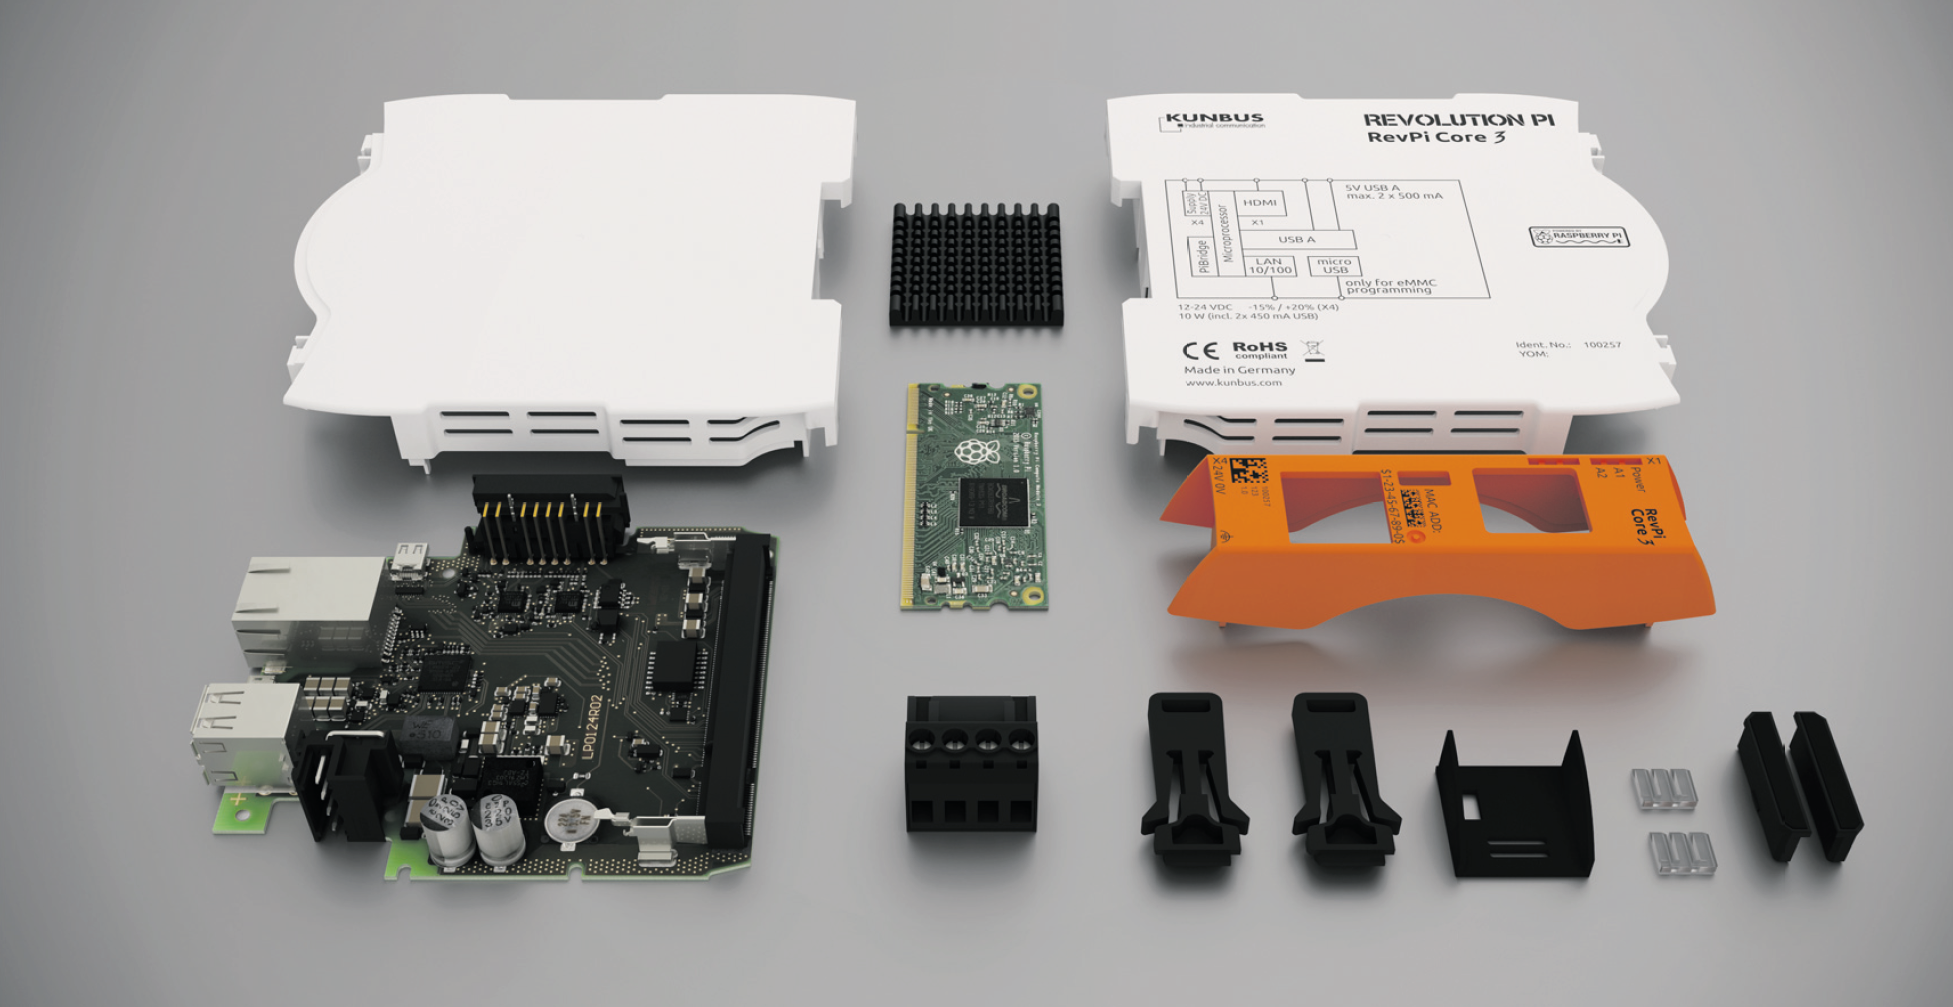
\includegraphics[width=0.85\textwidth]{doc/tex/images/revpi_teardown.png}
    \caption{Der RevPi Core 3 und seine Einzelkomponenten (Quelle: Kunbus)
      \label{fig:revpi-expl}}
\end{figure}

Spezifikationen des RevPi Core 3 \citep[Auswahl, vgl.][S. 1]{datasheet-revpi}:
\begin{itemize}
  \item{Prozessor: BCM2837}
  \item{Taktfrequenz 1,2 GHz}
  \item{Anzahl Prozessorkerne: 4}
  \item{Arbeitsspeicher: 1 GByte}
  \item{eMMC Flash Speicher: 4 GByte}
  \item{Betriebssystem: Angepasstes Raspbian mit RT-Patch}
  \item{RTC mit 24h Pufferung über wartungsfreien Kondensator}
  \item{Treiber / API: Kernel-Treiber schreibt zyklisch Prozessdaten in ein Prozessabbild, Zugriff auf Prozessabbild mittels ioctl-Anfragen oder über Linux-Dateisystem als API zu Fremdsoftware}
  \item{Kommunikationsanschlüsse: 2 x USB 2.0 A, 1 x Micro-USB, HDMI, Ethernet 10/100 Mbit/s}
  \item{Stromversorgung: min. 10,7 V, max. 28,8 V, maximal 10 Watt}
\end{itemize}

Kunbus stellt für den Revolution Pi ein auf Raspbian\footnote{Raspbian ist eine speziell 
für den Raspberry Pi angepasste Variante von Debian.} Stretch basierendes Betriebssystem bereit.
Verwendet wird der Kernel 4.9.76-rt60-v7+ in Verbindung mit dem SMP PREEMPT RT Patch.

\begin{figure}
    \centering
    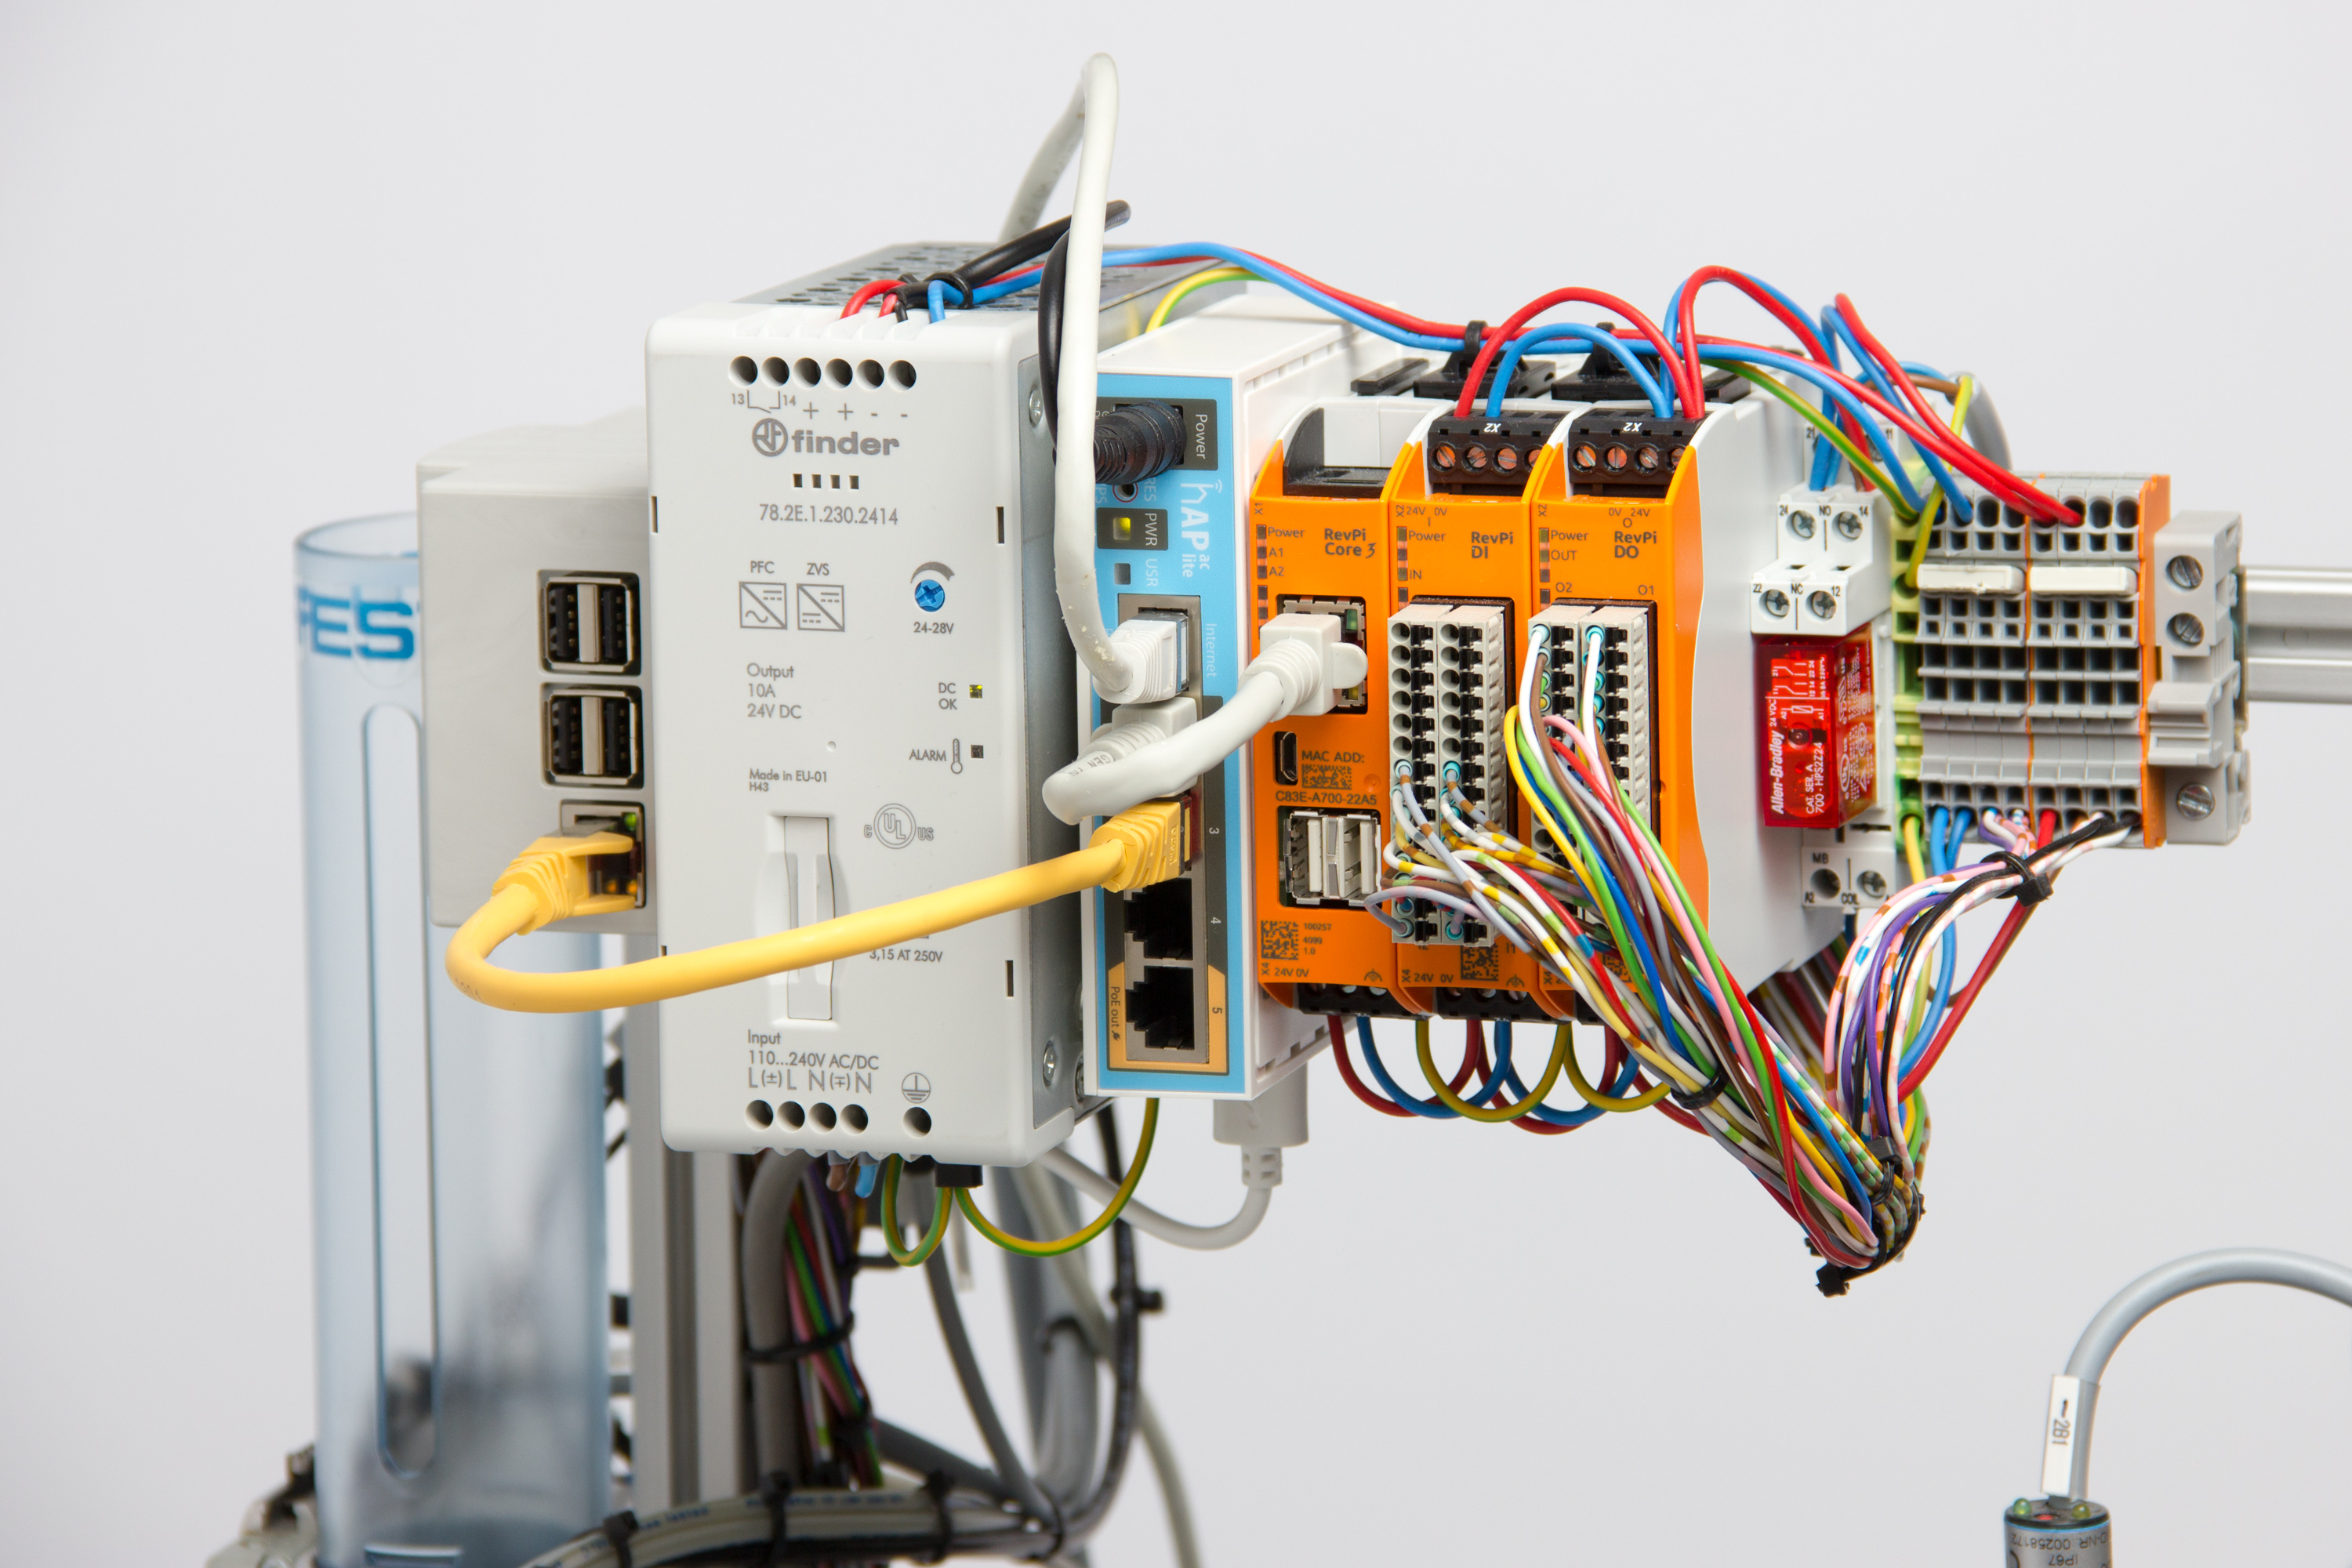
\includegraphics[trim={13cm 5cm 1cm 3cm}, clip, width=0.85\textwidth]{../photos/serverless_plc_img_8}
    \caption{Der Revolution Pi 3 mit digitalen IO-Modulen}
    \label{fig:rev-pi-io}
\end{figure}

Kunbus bietet neben dem sog. Core auch IO- und Gateway-Modulen zur Erweiterung der SPS an, siehe Bild~\ref{fig:rev-pi-io}.
Gateways dienen der Kommunikation mit externen Systemen oder Komponenten
über in der Automatisierungstechnik gängige Protokolle wie PROFIBUS oder EtherCAT. 
IO-Module erlauben die Überwachung und Steuerung von digitalen oder analogen Ein- und Ausgängen (IOs).

Kunbus deklariert die Hardware des Revolution Pi als Open-Source \citep[vgl.][S. 4]{flyer-revpi}. 
Die Schaltpläne des Revolution Pi, genauer die des RevPi Core 3 und der IO-Module, stehen auf der
Website\footnote{\label{downloads}\url{https://revolution.kunbus.com/tutorials/downloads/}} des Herstellers zum 
Download bereit. Eine Lizenz wird nicht angegeben.
Die Raspberry Pi Foundation stellt die Schaltpläne des Compute Modules des weiteren in ihrem Gitub-Repository 
zum Download bereit.

Sowohl die Raspberry Pi Foundation als auch die Kunbus GmbH pflegen aktiv ihre öffentlichen Repositories\footnote{\url{https://github.com/raspberrypi/} resp.~\url{https://github.com/RevolutionPi/}}
auf Github. 

% Kunbus konnte so einige Verbesserungen zum Linux Kernel 4.15 beitragen
% \footnote{siehe \url{https://revolution.kunbus.com/our-contribution-to-linux-4-15/}}.
% \todo{letzten Absatz evtl. weglassen? an sich nicht schlecht, passt aber irgendwie 
% nicht richtig zum Rest und stört den Lesefluss}

\subsubsection{Zugriff auf IO-Module%
        \label{sec:2-io}}
Der Zugriff auf die Ein- und Ausgänge der IO-Module erfolgt über einen RS485-Bus und einen in Form eines Kernel-Moduls bereitgestellten Treiber, genannt piControl. Der RS485-Bus ist über die serielle Schnittstelle des Compute Modules angebunden. 
piControl stellt ein Prozessabbild bereit, welches den physikalischen Zustand der Ein- und Ausgänge der IO-Module repräsentiert.
Das Prozessabbild wird, wie in der Automatisierungstechnik üblich, zyklisch aktualisiert. 
Die angestrebte Zykluszeit beträgt 5ms, kann jedoch je nach Anzahl der angeschlossenen Module auch größer sein. 
Kunbus garantiert bei drei IO-Modulen und zwei Gateway-Modulen eine Zykluszeit von 10 ms \citep[vgl.][]{web-revpi-dio}.
Die garantierte Zykluszeit ermöglicht die Umsetzung von Anwendungen mit harten Echtzeit-Anforderungen.

Fremdanwendungen können über eine Applikationsschnittstelle (API) auf das Prozessabbild zugreifen. 
Hierzu stellt das Kernel-Modul piControl sowohl \lstinline{seek}, \lstinline{read} und \lstinline{write} Methoden zur verfügung, wie auch die Möglichkeit mittels \lstinline{ioctl}-Anfragen gezielt auf einzelne Variablen des Prozessabbildes zuzugreifen.
In der englischsprachigen Wikipedia werden ioctl-Aufrufe wie folgt beschrieben:

\glqq{}The kernel is designed to be extensible, and may accept an extra module called a device driver which runs in kernel space and can directly address the device. An ioctl interface is a single system call by which userspace may communicate with device drivers. [...] The basic kernel can thus allow the userspace to access a device driver without knowing anything about the facilities supported by the device, and without needing an unmanageably large collection of system calls.

[...] ioctl calls provide a convenient way to bridge userspace code to kernel extensions. Kernel extensions can provide a location in the filesystem that can be opened by name, through which an arbitrary number of ioctl calls can be dispatched, allowing the extension to be programmed without adding system calls to the operating system.\grqq{}\citep[vgl.][]{web-wiki-ioctl}

Der Quellcode von piControl steht unter der GNU General Public License Version 2 (GNU GPLv2) und ist 
auf Github verfügbar\footnote{\url{https://github.com/RevolutionPi/piControl}}. Als Einstieg in die 
Entwicklung eigener Steuerungsprogramme liefert Kunbus das C-Programm piTest mit. Dieses verwendet 
piControl und erlaubt dem Nutzer über Kommandozeilen-Parameter die angeschlossenen IO-Module zu steuern.

\begin{figure}[h]
    \centering
    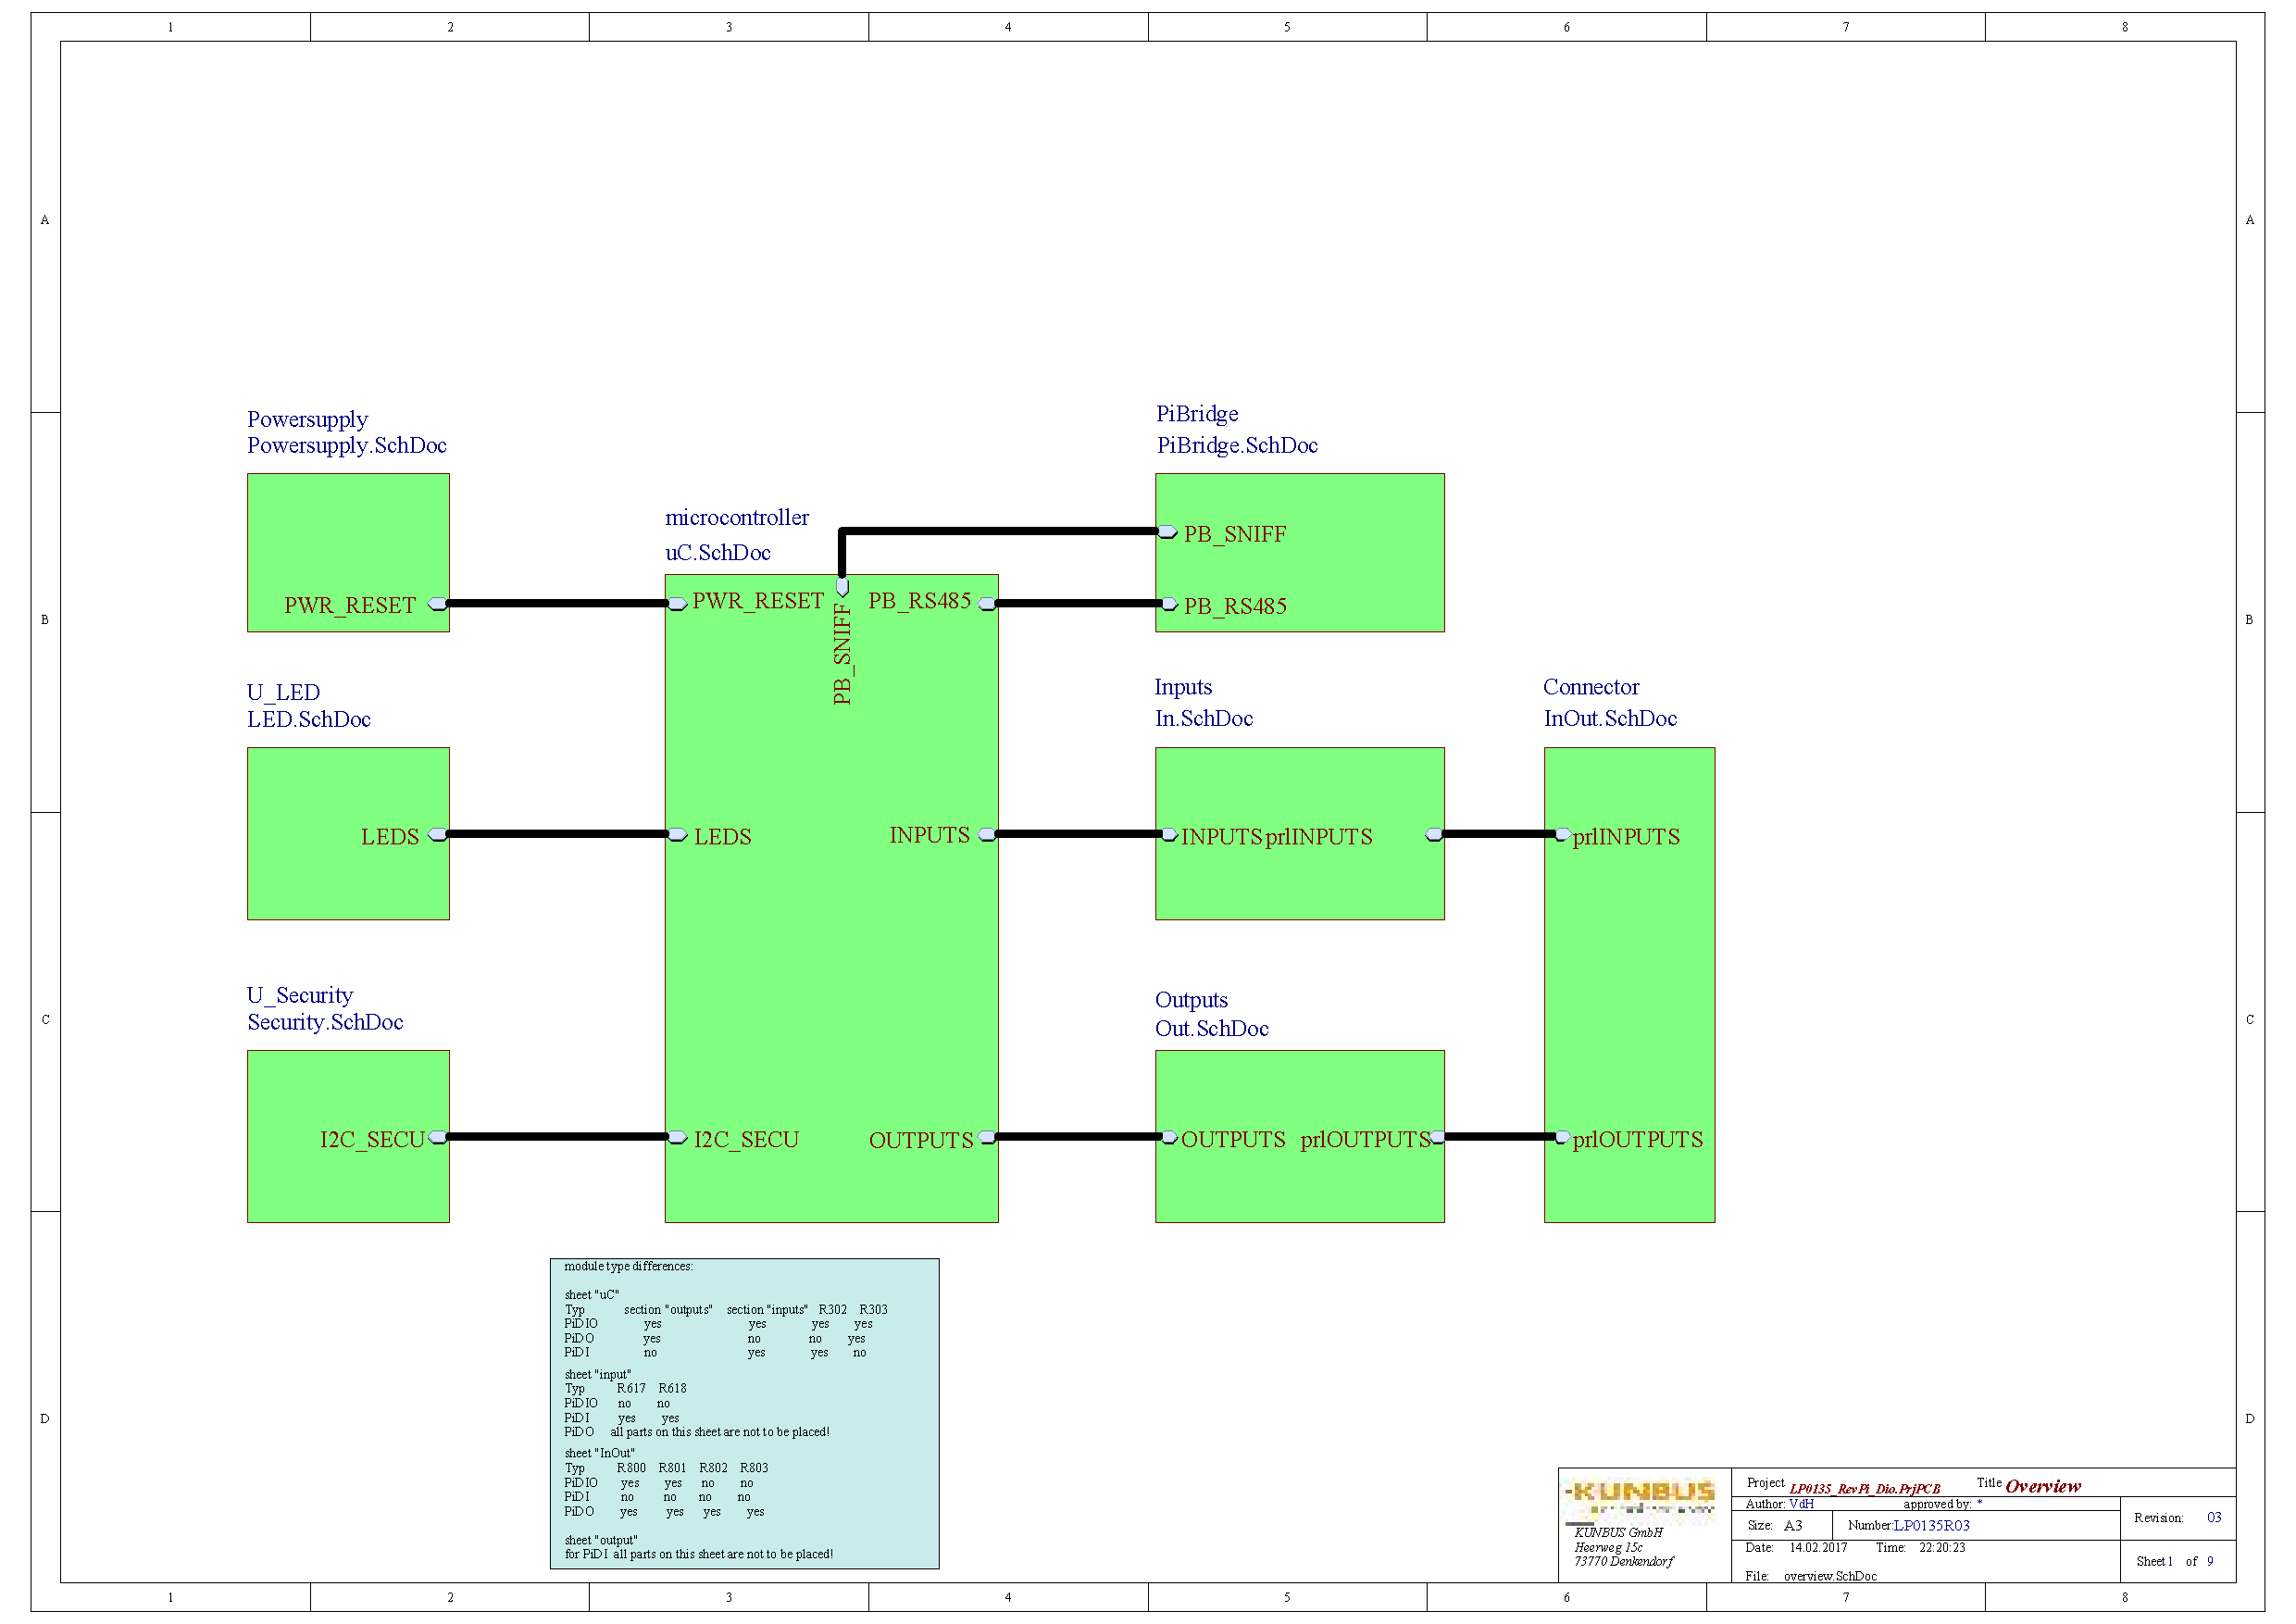
\includegraphics[trim={4cm 7cm 10.5cm 7.3cm}, clip, width=\textwidth]{literature/SchematicPrintsRevPi-DIO}
    \caption{Schematische Darstellung eines DIO-Moduls (Quelle: Kunbus\textsuperscript{\ref{downloads}})
      \label{fig:dio}}
\end{figure}

Jedes der IO-Module stellt ein eigenständiges eingebettetes System dar. Es verfügt
über einen Microcontroller, welcher die IOs bereitstellt und über einen RS485-Bus
mit dem Revolution Pi kommuniziert (siehe Bild~\ref{fig:dio}). 
Kunbus stellt exemplarisch den Quellcode eines DIO-Moduls unter der MIT Lizenz zur
Verfügung\footnote{\url{https://github.com/RevolutionPi/IODeviceExample}}. 


\subsection{Echtzeit und Multitasking unter Linux -- preemptRT und posix%
     \label{sec:2-echtzeit}}
     
Moderne Betriebssysteme realisieren Multitasking i.d.R.\,in Form des präemptiven Multitasking. 
Der Kernel verfügt über einen sog. Scheduler. Dieser priorisiert alle Prozesse und weist ihnen 
Rechenzeit in sog. Time Slots zu. Die Größe der Zeitfenster sowie die Ausführungsreihenfolge 
ist von der Priorität eines Prozesses abhängig. Besonders an einem präemptiven im Gegensatz zu einem kooperativen Scheduler ist dessen Fähigkeit, Tasks während ihrer Ausführung zu unterbrechen bzw. zu pausieren, wenn diese eine bestimmte Dauer überschreiten oder ein höher priorisierter Prozess (bspw. ausgelöst durch einen Interrupt oder durch eine inhärente Periodizität) Rechenleistung benötigt.

Eine Sonderform des präemptiven Multitasking ist das präemptible Multitasking. Hierbei werden auch Teile 
des Kernels als Threads durch den Scheduler ausgeführt. Dieser ist somit in der Lage, auch Prozesse des Kernels
zu unterbrechen, wenn andere Anwendungen Prozessorzeit oder Zugriff auf andere Systemressourcen benötigen
\citep[vgl.][]{web-wiki-praempt}.
     
Der Linux-Kernel implementiert unterschiedliche Präemptions-Modelle \citep[vgl.][/preemption\_models]{web-linuxwiki-basics}:

\begin{itemize}
  \item No Forced Preemption (server):
  Ausgelegt auf maximal möglichen Durchsatz, lediglich Interrupts und
  System-Call-Returns bewirken Präemption.

  \item Voluntary Kernel Preemption (Desktop):
  Neben den implizit bevorrechtigten Interrupts und System-Call-Returns gibt es
  in diesem Modell weitere Abschnitte des Kernels in welchen Preämption explizit
  gestattet ist.

  \item Preemptible Kernel (Low-Latency Desktop):
  In diesem Modell ist der gesamte Kernel, mit Ausnahme sog.~kritischer Abschnitte
  präemptible. Nach jedem kritischen Abschnitt gibt es einen impliziten Präemptions-Punkt.

  \item Preemptible Kernel (Basic RT):
  Dieses Modell ist dem zuvor genannten sehr ähnlich, hier sind jedoch alle Interrupt-Handler
  als eigenständige Threads ausgeführt.

  \item Fully Preemptible Kernel (RT):
  Wie auch bei den beiden zuvor genannten Modellen ist hier der gesamte Kernel
  präemtible. Die Anzahl und Dauer der nicht-präemtiblen kritischen Abschnitte
  ist auf ein notwendiges Minimum beschränkt. Alle Interrupt-Handler sind als
  eigenständige Threads ausgeführt, Spinlocks durch Sleeping-Spinlocks und Mutexe
  durch sog.~RT-Mutexe ersetzt.

\end{itemize}

Lediglich ein präemtibler Kernel kann hartes Echtzeit-Verhalten realisieren, 
da nur hier eine maximale Antwortzeit garantiert werden kann.
Viele Prozesse in der Automatisierungstechnik erfordern harte Echtzeit. 
Eine verspätete Antwort auf eine Anfrage, 
wie etwa das Signal eines Lagenendschalters oder eines Notausschalters kann hier nicht nur über
den Erfolg eines Prozesses, sondern auch über das Leben der daran beteiligten Mitarbeiter entscheiden.
Für weiterführende Erklärungen bzgl.\,Echtzeit, Mutexen und 
Spinlocks sei an dieser Stelle auf die Vorlesung verwiesen~\citep{script-peter}.


\subsubsection{preemptRT%
        \label{sec:2-preemptRT}}

Der Kernel des auf dem Revolution Pi installierten Raspbian mit PREEMP\_RT Patch fällt 
in die Kategorie des \glqq{}Fully Preemptible Kernels\grqq{} (siehe Abschnitt \ref{sec:2-echtzeit}).
Das zugrunde liegende Prinzip lässt sich wie folgt formulieren: Nur Code, welcher absolut nicht-präemtible sein darf, ist es
gestattet nicht-präemtible zu sein. Ziel ist folglich, die Menge des nicht-präemtiblen 
Codes im Linux-Kernel auf das absolut notwendige Minimum zu reduzieren.

Dies wird durch Verwendung folgender Mechanismen erreicht~\citep[vgl.][]{web-linuxwiki-details}:

\begin{itemize}
  \item Hochauflösende Timer
  \item Sleeping Spinlocks
  \item Threaded Interrupt Handlers
  \item rt\_mutex
  \item RCU
\end{itemize}

Diese Mechanismen sind bspw. im Linux-Wiki\footnote{siehe \url{https://wiki.linuxfoundation.org/realtime/documentation/technical_details}} ausführlich beschrieben.

\subsubsection{POSIX%
        \label{sec:2-posix}}
Das Portable Operating System Interface (POSIX) bezeichnet eine Sammlung von Standards, 
welche auf dem Unix-System basieren, jedoch nicht auf dieses beschränkt sind.

Der Wechsel zwischen verschiedenen Unix-Distributionen brachte oft Kompatibilitätsprobleme mit sich. 
Dieser Mangel an Portabilität erschwerte Benutzern und Entwicklern die Verwendung bzw. Bereitstellung 
von Software auf unterschiedlichen Systemen. 
Das Institut für Elektrotechnik und Elektronik (IEEE) begann 1984 mit der Entwicklung des Unix-Standards.
Sie entwickelten das, was heute als Single UNIX Specification bekannt ist und allgemein als POSIX bezeichnet wird~\citep[vgl.][]{web-debianwiki-posix}.
Das Konsortium \glqq{}The Open Group\grqq{} überwacht die weitere Entwicklung dieses Standards.
Ferner stellt es einen Teil der POSIX-Spezifikation frei zur Verfügung~\citep[vgl.][]{web-opengroup-posix}.

Die aktuelle Version POSIX.1-2017 ist verfügbar als IEEE Standard 1003.1-2017 sowie in Form der \glqq{}The Open Group Technical Standard Base Specifications\grqq{}, Ausgabe 7. POSIX.1-2017 definiert eine Standard-Betriebssystemschnittstelle und -umgebung, einschließlich eines Befehlsinterpreters (auch Shell genannt) und gängiger Dienstprogramme zur Unterstützung der Portabilität von Anwendungen auf Quellcode-Ebene. POSIX.1-2017 ist sowohl für Anwendungsentwickler als auch für Systemimplementierer gedacht und umfasst vier Hauptkomponenten \citep[vgl.][]{web-opengroup-overview}:
\begin{itemize}
    \item Basisdefinitionen:\\
          Allgemeine Begriffe, Konzepte und Schnittstellen einschließlich Hilfskonventionen und C-Headern
          
    \item Systemschnittstellen:\\
          Definitionen für Systemdienstfunktionen und Unterprogramme, C-spezifische Systemdienste, Portabilität
        
    \item Shell und Dienstprogramme:\\
          Definitionen für eine Schnittstelle zur Befehlsinterpretation von Diensten und gängige Hilfsprogramme
    
    \item Begründungen und Historie
\end{itemize}

Debian basiert auf Linux und verwendet den Linux-Kernel. Linux ist zu großen Teilen POSIX-kompatibel. Debian ist jedoch nicht POSIX-zertifiziert, da diese Zertifizierung mit hohen Kosten verbunden ist\citep[vgl.][Kapitel 4.4.]{web-debian-faq}.

Beide Kernkomponenten des in dieser Arbeit vorgestellten Projektes nutzen Komponenten von Linux, 
welche an den POSIX-Standard angelehnt sind: open62541 verwendet u.a.\,POSIX-Threads und
Mutexe~\citep[vgl.][pthread.h]{web-opengroup-pthread}, piControl nutzt POSIX-Semaphoren
\citep[vgl.][semaphore.h]{web-opengroup-semaphore}. 


\subsection{OPC-UA und open62541%
     \label{sec:2-opc}}
In diesem Abschnitt sollen Möglichkeiten des Datenaustausch zwischen Komponenten der
Automatisierungstechnik vorgestellt werden. OPC-UA stellt einen offenen, IP-basierten Kommunikationsstandard
für Sensoren und Steuerungen dar. open62541 ist eine freie Client- sowie Server-Implementierung dieses
Standards, geschrieben in C.


\subsubsection{OPC UA%
        \label{sec:2-opcua}}

Open Platform Communications (OPC) ist eine Familie von Standards zur herstellerunabhängigen
Kommunikation von Maschinen (M2M) in der Automatisierungstechnik. Die sog. OPC Task Force, zu deren
Mitgliedern verschiedene etablierte Firmen der Automatisierungsindustrie gehören, veröffentlichte
die OPC Specification Version 1.0 im August 1996.
Motiviert ist dieser offene Standard durch die Erkenntniss, dass die Anpassung der
zahlreichen Herstellerstandards an individuelle Infrastrukturen und Anlagen einen
großen Mehraufwand verursachen.
Die Wikipedia beschreibt das Anwendungsgebiet für OPC wie folgt \citep[vgl.][]{web-wiki-opc}:

\glqq{}OPC wird dort eingesetzt, wo Sensoren, Regler und Steuerungen verschiedener Hersteller
ein gemeinsames Netzwerk bilden. Ohne OPC benötigten zwei Geräte zum Datenaustausch
genaue Kenntnis über die Kommunikationsmöglichkeiten des Gegenübers. Erweiterungen
und Austausch gestalten sich entsprechend schwierig. Mit OPC genügt es, für jedes
Gerät genau einmal einen OPC-konformen Treiber zu schreiben. Idealerweise wird
dieser bereits vom Hersteller zur Verfügung gestellt. Ein OPC-Treiber lässt sich
ohne großen Anpassungsaufwand in beliebig große Steuer- und Überwachungssysteme
integrieren.

OPC unterteilt sich in verschiedene Unterstandards, die für den jeweiligen Anwendungsfall
unabhängig voneinander implementiert werden können. OPC lässt sich damit verwenden
für Echtzeitdaten (Überwachung), Datenarchivierung, Alarm-Meldungen und neuerdings
auch direkt zur Steuerung (Befehlsübermittlung).\grqq{}

OPC basiert in der ursprünglichen Spezifikation (auch als OPC DA bezeichnet) auf Microsofts DCOM-Spezifikation.
DCOM macht Funktionen und Objekte einer Anwendung anderen Anwendungen im Netzwerk
zugänglich. Der OPC-Standard definiert entsprechende DCOM-Objekte um mit anderen
OPC-Anwendungen Daten austauschen zu können. Die Verwendung von DCOM bindet Anwender
jedoch an Betriebssysteme von Microsoft. 

\begin{figure}
    \centering
    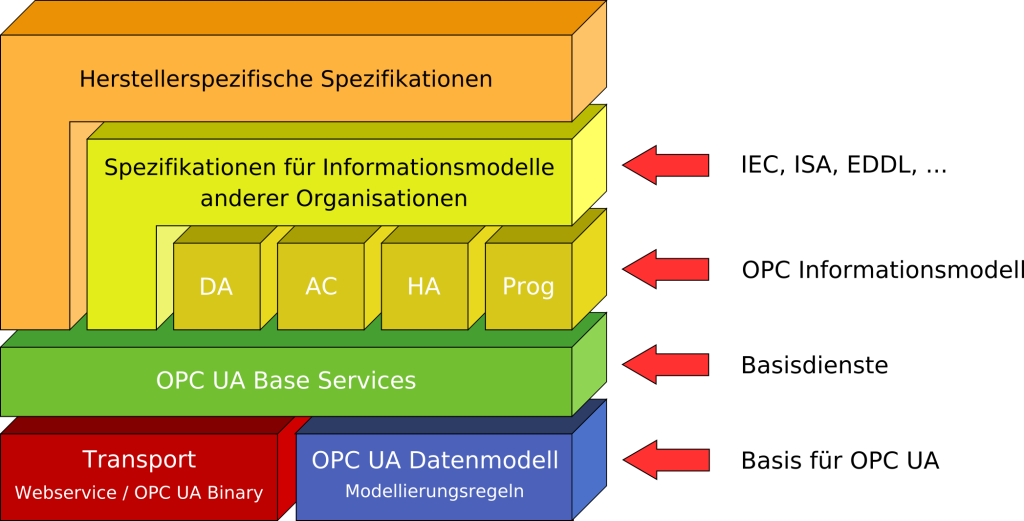
\includegraphics[width=0.85\textwidth]{images/UA_Architecture_1024.png}
    \caption{Die OPC Unified Architecture. Grafik von Gerhard Gappmeier - ascolab GmbH, CC BY-SA 3.0}
    \label{fig:opc-unified-architecture}
\end{figure}
% Evtl Grafik: Von Gerhard Gappmeier - ascolab GmbH, CC BY-SA 3.0, https://de.wikipedia.org/w/index.php?curid=1892069

Die ursprüngliche OPC Spezifikation wurde 2006 durch die Entwicklung der 
OPC Unified Architecture (OPC UA) überholt. 
Diese zeichnet sich durch eine Service-orientierte Architektur (SOA) aus, deren Struktur
aus mehreren Schichten besteht, siehe Abbilung~\ref{fig:opc-unified-architecture}. 
Über der untersten Schicht, dem Betriebssystem des Servers, verbindet eine Portabilitäts-Schicht 
den sog.\, UA ANSI C Stack mit einer API. Diese API kann bspw.\,in C++ geschrieben sein, 
und erlaubt die Anbindung der obersten Schicht, der Anwendungsschicht~\citep[vgl.][]{web-spec-opc}.
OPC UA setzt auf einem eigenen Kommunikationsstack auf; die Verwendung von DCOM
und damit die Bindung an Microsoft wurden aufgelöst.

Neben Architektur und Kommunikationsschnittstellen wird in der OPC Spezifikation auch ein 
Informationsmodell definiert. Die deutschsprachige Wikipedia beschreibt dieses wie folgt: 

\glqq{}Das OPC[-UA]-Informationsmodell ist nicht mehr nur eine Hierarchie aus Ordnern, Items
und Properties. Es ist ein sogenanntes Full-Mesh-Network aus Nodes, mit dem neben
den Nutzdaten eines Nodes auch Meta- und Diagnoseinformationen repräsentiert werden. [...]
Ein Node ähnelt einem Objekt aus der objektorientierten Programmierung. Ein Node
kann Attribute besitzen, die gelesen werden können. Es ist möglich Methoden zu definieren und aufzurufen. [...]
Weiterhin werden Events unterstützt, die versendet werden können
(AE (Alarms \& Events), DA DataChange), um bestimmte Informationen zwischen Geräten
auszutauschen. Ein Event besitzt unter anderem einen Empfangszeitpunkt, eine Nachricht
und einen Schweregrad. Die o.\,g. Nodes werden sowohl für die Nutzdaten als auch
alle anderen Arten von Metadaten verwendet. Der damit modellierte OPC-Adressraum
beinhaltet nun auch ein Typmodell, mit dem sämtliche Datentypen spezifiziert werden.\grqq{}


\subsubsection{open62541%
        \label{sec:2-open62541}}
open62541 ist eine offene und freie Implementierung von OPC UA. 
Die in C geschriebene Bibliothek stellt eine beständig zunehmende Anzahl der im OPC UA Standard definierten
Funktionen bereit. Sie kann sowohl zur Erstellung von OPC-Servern als auch von -Clients
genutzt werden. Ergänzend zu der unter der Mozilla Public License v2.0 lizensierten
Bibliothek stellt das open62541 Projekt auch Beispielprogramme unter einer CC0 Lizenz
zur Verfügung.
Zu den Unterstützern des Projektes zählen u.a.\, die RWTH Aachen, das Frauenhofer IOSB sowie die TU Dresden.

Die Bibliothek eignet sich auch für die Entwicklung auf eingebetteten Systemen und
Microcontrollern. Die Größe einer Server-Binary kann weniger als 100kB betragen.

Folgende Auswahl an Eigenschaften und Funktionen zeichnet die in dieser Arbeit verwendete
Version 0.3 von open62541 aus:
\begin{itemize}
  \item Kommunikationionsstack
  \begin{itemize}
      \item OPC UA Binär-Protokoll (HTTP oder SOAP werden gegenwärtig nicht unterstützt)
      \item Austauschbare Netzwerk-Schicht, welche die Verwendung eigener Netzwerk-APIs
      erlaubt.
      \item Verschlüsselte Kommunikationion
      \item Asynchrone Dienst-Anfragen im Client
  \end{itemize}
  \item Informationsmodell
  \begin{itemize}
    \item Unterstützung aller OPC UA Node-Typen, inkl.~Methoden
    \item Hinzufügen und Entfernen von Nodes und Referenzen zur Laufzeit.
    \item Vererbung und Instanziierung von Objekt- und Variablentypen
    \item Zugriffskontrolle auch für einzelne Nodes
  \end{itemize}
  \item Subscriptions
  \begin{itemize}
    \item Erlaubt die Überwachung (subscriptions / monitoreditems)
    \item Sehr geringer Ressourcenbedarf pro überwachtem Wert
  \end{itemize}
  \item Code-Generierung auf XML-Basis
  \begin{itemize}
    \item Erlaubt die Erstellung von Datentypen
    \item Erlaubt die Generierung des serverseitigen Informationsmodells
  \end{itemize}
\end{itemize}

Weiterführende Informationen und Code-Beispiele bietet die ausführliche Dokumentation des Projektes~\citep[siehe]{web-open62541} sowie der kommentierte Quelltext.

%% % Imports nur für Referenzenauflösung während des Schreibens! Vorm Kompilieren auskommentieren!
% \bibliography{0_hauptdatei}
% \input{1_einleitung}
% \input{2_grundlagen}
% \input{3_konzeption}
% \input{4_implementierung}
% \input{5_tests}
% \input{6_zusammenfassung}
% \input{anhang}
% % Ende Imports

\section{Systemkonzept%
  \label{sec:3-konzeption}}
Auf Basis der in Abschnitt [...] vorgestellten Möglichkeiten folgt nun die Ausarbeitung eines Konzepts.

\subsection{Anbindung der IO an den OPC-Server%
     \label{sec:3-anbindung}}

\subsection{Integration des OPC-Servers in das System%
     \label{sec:3-integration}}

%% % Imports nur für Referenzenauflösung während des Schreibens! Vorm Kompilieren auskommentieren!
% \bibliography{0_hauptdatei}
% \input{1_einleitung}
% \input{2_grundlagen}
% \input{3_konzeption}
% \input{4_implementierung}
% \input{5_tests}
% \input{6_zusammenfassung}
% \input{anhang}
% % Ende Imports

\section{Implementierung%
  \label{sec:4-implementierung}}
Das folgende Kapitel stellt in Auszügen die Implementierung des OPC-Servers sowie die Anbindung an die IO-Module
der SPS dar. Der Schwerpunkt liegt hierbei auf der Funktionsweise des piControl-Treibers und dessen Integration in das Projekt. Abschnitt~\ref{sec:4-picontrol} erklärt die zum Schreibens eines Bits verwendeten Funktionsaufrufe.
Zuvor soll jedoch in Abschnitt~\ref{sec:4-open62541} der Teil des OPC-Servers vorgestellt werden, welcher auf besagten Treiber zugreift. 

\subsection{Implementierung des OPC-Servers%
     \label{sec:4-open62541}}
Wie im vorangegangenen Abschnitt~\ref{sec:3-integration} begründet, soll die Verknüpfung zwischen dem Prozessabbild der SPS und den auf dem OPC-Server bereitgestellten Werten über sog.\,Datenquellen erfolgen. Hierzu ist zunächst eine Callback-Methode zu implementieren, welche bei einem Lese- oder Schreibzugriff auf eine Variable aufgerufen wird. Die Verknüpfung zwischen Callback-Methode und Variable muss manuell erfolgen.

\begin{lstlisting}[language={c},firstnumber=237,caption={Auszug der Methode \lstinline{linkDataSourceVariable} in \lstinline{variables.c}\label{lst:4-linkDataSourceVariable}}]
extern UA_StatusCode
 linkDataSourceVariable(UA_Server *server, UA_NodeId nodeId) {
     bool readonly = false;
     UA_DataSource dataSourceVariable;
     UA_StatusCode rc; |>\setcounter{lstnumber}{254}<|

     dataSourceVariable.read = readDataSourceVariable;
     if (!readonly)
        dataSourceVariable.write = writeDataSourceVariable;
     else
        dataSourceVariable.write = writeReadonlyDataSourceVariable;

     return UA_Server_setVariableNode_dataSource(server, nodeId, dataSourceVariable);
 }
\end{lstlisting}

\begin{figure}[h]
    \centering
    \includegraphics[width=0.42\textwidth]{doc/img/OPC_RevPiDO.pdf}
    \caption{Auszug des verwendeten Nodesets, hier Digitalausgang 1 des Versuchsaufbaus
      \label{fig:opc-do}}
\end{figure}

Die in Listing~\ref{lst:4-linkDataSourceVariable} abgebildete Methode \lstinline{linkDataSourceVariable()} erzeugt ein Struct vom Typ \lstinline{UA_DataSource}. In diesem werden dem Lesen und Schreiben einer OPC-Variablen entsprechende Callback-Methoden zugewiesen. Die Verknüpfung einer OPC-Variable, genauer ihrer NodeId, mit der zuvor definierten Datenquelle erfolgt über die von open62541 bereitgestellte Methode \lstinline{UA_Server_setVariableNode_dataSource()}. Vor dem Lesen und nach dem Schreiben dieser Variable werden von nun an die entsprechenden Callbacks aufgerufen.
     
\begin{lstlisting}[language={c},firstnumber=168,caption={Auszug des Callbacks \lstinline{writeDataSourceVariable} in \lstinline{variables.c}\label{lst:4-writeDataSourceVariable}}]  
extern UA_StatusCode
 writeDataSourceVariable(UA_Server *server,
            const UA_NodeId *sessionId, void *sessionContext,
            const UA_NodeId *nodeId, void *nodeContext,
            const UA_NumericRange *range, const UA_DataValue *dataValue) {

    UA_StatusCode retval  = UA_STATUSCODE_GOOD;
    UA_NodeId *nameNodeId = UA_malloc(sizeof(UA_NodeId));
    UA_QualifiedName nameQN = UA_QUALIFIEDNAME(1, "Name");
    UA_Variant nameVar;
    UA_Boolean bit;

    retval |= findSiblingByBrowsename(server, nodeId, &nameQN, nameNodeId);
    retval |= UA_Server_readValue(server, *nameNodeId, &nameVar);
    retval |= UA_Boolean_copy(dataValue->value.data, &bit);

    |>\tikzmarkin[set border color=martinired]{writeIO}<|PI_writeSingleIO(String_fromUA_String(nameVar.data), &bit, false);                                                 |>\tikzmarkend{writeIO}<|

    free(nameNodeId);
    return retval;
 }
\end{lstlisting}

Listing~\ref{lst:4-writeDataSourceVariable} zeigt die Callback-Methode, welche nach dem Schreiben einer Variablen auf dem OPC-Server aufgerufen wird.
Dieser Methode wird neben der NodeId der mit ihr verknüpften Variablen auch der Wert dieser in Form eines Zeigers auf ein Struct vom Typ \lstinline{UA_DataValue} übergeben.

Die Gestaltung des hier verwendeten Nodesets sieht vor, dass in einer OPC-Variablen \lstinline{"Name"} der Bezeichner des zu schreibenden Digitalausgangs hinterlegt ist, siehe Abbildung~\ref{fig:opc-do}. Dies erlaubt eine Rekonfiguration der Ein- und Ausgänge der SPS ohne Änderungen im Programmcode des OPC-Servers vornehmen zu müssen.
Es ist daher erforderlich, nach jedem Schreiben einer mit einem Digitalausgang verknüpften Variablen, hier \lstinline{"Value"}, dessen Bezeichner \lstinline{"Name"} abzufragen. 
Dies geschieht in den Zeilen 180 und 181.
Anschließend wird dieser Bezeichner sowie der zu schreibende Wert der Methode \lstinline{PI_writeSingleIO()} übergeben, welche wiederum die Interaktion mit piControl übernimmt (vgl. Abschnitt \ref{sec:4-picontrol}).
 
\subsection{Integration von piControl%
     \label{sec:4-picontrol}}
In Abschnitt~\ref{sec:2-io} wurde die Anbindung der IO-Module des Revolution Pi sowie die Funktionsweise von piControl aus Anwendersicht beschrieben. Die verfügbare Literatur beschränkt sich auch auf lediglich diese Sicht; eine weiterführende Dokumentation für Entwickler gibt es, neben der in Abschnitt~\ref{sec:3-anbindung} vorgestellten Manpage, nicht. 
In diesem Abschnitt soll daher der Quellcode von piControl sowie dessen Verwendung im Projekt genauer betrachtet werden.
Hierzu wird exemplarisch die in Abschnitt~\ref{sec:4-open62541} eingeführte Methode \lstinline{PI_writeSingleIO()} untersucht.
Diese Methode ermöglicht das Setzen eines einzelnen Bits im Prozessabbild der SPS, und damit das Schalten eines digitalen Ausgangs auf einem IO-Modul.
Die äquivalente Methode \lstinline{int piControlGetBitValue(SPIValue *pSpiValue)} zum Lesen eines Bits bzw. Eingangs funktioniert analog und soll daher an dieser Stelle nicht dediziert erörtert werden.

\begin{lstlisting}[language={c},firstnumber=97,
                   caption={Setzen eines phsikalischen, digitalen Ausgangs in \lstinline{revpi.c}
                   \label{lst:4-PI_writeSingleIO}}]
extern void PI_writeSingleIO(char *pszVariableName, bool *bit, bool verbose)
{
	int rc;
	SPIVariable sPiVariable;
	SPIValue sPIValue;

	strncpy(sPiVariable.strVarName, pszVariableName, sizeof(sPiVariable.strVarName));
	rc = piControlGetVariableInfo(&sPiVariable);
	if (rc < 0) {
		printf("Cannot find variable '%s'\n", pszVariableName);
		return;
	}

		sPIValue.i16uAddress = sPiVariable.i16uAddress;
		sPIValue.i8uBit = sPiVariable.i8uBit;
		sPIValue.i8uValue = *bit;
		rc = |>\tikzmarkin[set border color=martinired]{setBitValue}<|piControlSetBitValue(&sPIValue)|>\tikzmarkend{setBitValue}<|;
		if (rc < 0)
			printf("Set bit error %s\n", getWriteError(rc));
		else if (verbose)
			printf("Set bit %d on byte at offset %d. Value %d\n", sPIValue.i8uBit, sPIValue.i16uAddress,
			       sPIValue.i8uValue);
}
\end{lstlisting}

Der Programmcode in Listing~\ref{lst:4-PI_writeSingleIO} ist Teil des implementierten OPC-Servers. In diesem wird auf zwei Funktionen des piControl-Treibers zugegriffen. 
Beiden Methoden wird als Argument ein Zeiger auf ein Struct vom Typ \lstinline{SPIValue} übergeben. Der im Struct abgelegte Name wird mittels \lstinline{piControlGetVariableInfo(&sPIValue)} zu einer Adresse im Prozessabbild aufgelöst. Diese wird in \lstinline{sPIValue.i16uAdress} gespeichert. Der Wert der Variablen wird anschließend mittels \lstinline{piControlSetBitValue(&sPIValue)} an dieser Adresse in das Prozessabbild geschrieben.

\begin{lstlisting}[language={c},firstnumber=309,caption={Methode \lstinline{piControlSetBitValue} in \lstinline{piControlIf.c}\label{lst:4-piControlSetBitValue}}]
int |>\tikzmarkin[set border color=martiniblue]{setBitValueFcn}<|piControlSetBitValue(SPIValue *pSpiValue)|>\tikzmarkend{setBitValueFcn}<|
{
    piControlOpen();

    if (PiControlHandle_g < 0)
	    return -ENODEV;

    pSpiValue->i16uAddress += pSpiValue->i8uBit / 8;
    pSpiValue->i8uBit %= 8;

    if (|>\tikzmarkin[set border color=martinired]{ioctl}<|ioctl(PiControlHandle_g, KB_SET_VALUE, pSpiValue)|>\tikzmarkend{ioctl}<| < 0)
	    return errno;

    return 0;
}
\end{lstlisting}

Die in Listing~\ref{lst:4-piControlSetBitValue} dargestellte Methode \lstinline{piControlSetBitValue} ist lediglich eine Hüllfunktion (häufig auch als Wrapper-Funktion bezeichnet) für einen Aufruf des \lstinline{ioctl} Kernel-Moduls.
Folgende Parameter werden übergeben:
\lstinline{PiControlHandle_g} ist die Referenz auf die Geräte-Datei des piControl-Treibers. \lstinline{KB_SET_VALUE} ist das ioctl-Kommando zum Schreiben eines Bits in das Prozessabbild. Der Zeiger \lstinline{pSpiValue} verweist auf ein Struct des bereits vorgestellten Typs \lstinline{SPIValue}.

\begin{lstlisting}[language={c},firstnumber=80,caption={Methode \lstinline{piControlOpen} in \lstinline{piControlIf.c}\label{lst:4-piControlOpen}}]
void piControlOpen(void)
{
    /* open handle if needed */
    if (PiControlHandle_g < 0)
    {
	    |>\tikzmarkin[set border color=martiniblue]{PiControlHandle}<|PiControlHandle_g = open(PICONTROL_DEVICE, O_RDWR)|>\tikzmarkend{PiControlHandle}<|;
    }
}
\end{lstlisting}

Die in Listing~\ref{lst:4-piControlOpen} dargestellte Methode öffnet, sofern nicht bereits geschehen, die Geräte-Datei. Das Macro \lstinline{PICONTROL_DEVICE} verweist hierbei auf \lstinline{/dev/piControl0}.

\begin{lstlisting}[language={c},firstnumber=721,caption={Methode \lstinline{piControlIoctl} in \lstinline{piControlMain.c}\label{lst:4-piControlIoctl}}]
static long |>\tikzmarkin[set border color=martiniblue, below offset=0.9em]{piControlIoctl}<|piControlIoctl(struct file *file, unsigned int prg_nr, 
                           unsigned long usr_addr)                                      |>\tikzmarkend{piControlIoctl}<|
{
  int status = -EFAULT;
  tpiControlInst *priv;
  int timeout = 10000;	// ms

  if (prg_nr != KB_CONFIG_SEND && prg_nr != KB_CONFIG_START && !isRunning()) {
  	return -EAGAIN;
  }

  priv = (tpiControlInst *) file->private_data;

  if (prg_nr != KB_GET_LAST_MESSAGE) {
  	// clear old message
  	priv->pcErrorMessage[0] = 0;
  }

  switch (prg_nr) {|>\setcounter{lstnumber}{864}<|

    case |>\tikzmarkin[set border color=martiniblue]{KB_SET_VALUE}<|KB_SET_VALUE:|>\tikzmarkend{KB_SET_VALUE}<|
  		{
  			SPIValue *pValue = (SPIValue *) usr_addr;

  			if (!isRunning())
  				return -EFAULT;

  			if (pValue->i16uAddress >= KB_PI_LEN) {
  				status = -EFAULT;
  			} else {
  				INT8U i8uValue_l;
  				my_rt_mutex_lock(&piDev_g.lockPI);
  				i8uValue_l = piDev_g.ai8uPI[pValue->i16uAddress];

  				if (pValue->i8uBit >= 8) {
  					i8uValue_l = pValue->i8uValue;
  				} else {
  					if (pValue->i8uValue)
  						i8uValue_l |= (1 << pValue->i8uBit);
  					else
  						i8uValue_l &= ~(1 << pValue->i8uBit);
  				}

  				|>\tikzmarkin[set border color=martinired]{i8uValue}<|piDev_g.ai8uPI[pValue->i16uAddress] = i8uValue_l;|>\tikzmarkend{i8uValue}<|
  				rt_mutex_unlock(&piDev_g.lockPI);

  #ifdef VERBOSE
  				pr_info("piControlIoctl Addr=%u, bit=%u: %02x %02x\n", pValue->i16uAddress, pValue->i8uBit, pValue->i8uValue, i8uValue_l);
  #endif

  				status = 0;
  			}
  		}
  		break; |>\setcounter{lstnumber}{1314}<|

    default:
      pr_err("Invalid Ioctl");
      return (-EINVAL);
      break;

    }

    return status;
  }
\end{lstlisting}

Listing~\ref{lst:4-piControlIoctl} zeigt in Auszügen die ioctl-Methode des piControl Kernel-Treibers. Diese bekommt folgende Argumente übergeben: \lstinline{struct file *file} enthält den Verweis auf die Geräte-Datei, hier \lstinline{/dev/piControl0}. Der Wert von \lstinline{unsigned int prg_nr} beschreibt die Anfrage an den Treiber, in diesem Fall \lstinline{KB_SET_VALUE}. Das Argument \lstinline{unsigned long usr_addr} enthält einen typ-agnostischen Pointer. Dieser verweist auf einen Speicherbereich, in welchem die zur Bearbeitung der Anfrage notwendigen Daten abgelegt sind. Hier können auch vom Treiber empfangene Daten dem Anwendungsprogramm bereitgestellt werden. 

Die switch-case-Anweisung führt die über das Argument \lstinline{prg_nr} spezifizierte Aktion aus. Hier betrachten wir \lstinline{KB_SET_VALUE}:
Zunächst wird in Zeile 868 der übergebene Zeiger \lstinline{usr_addr} mittels explizitem Typecast zu einem Zeiger des Typs \lstinline{SPIValue *} konvertiert. Da dieser auf Daten im Userspace verweist, ist beim Zugriff durch den Kernel-Treiber besondere Vorsicht geboten.
In Zeile 877 wird mittels Mutex das Prozessabbild \lstinline{piDev_g} für den Zugriff durch andere Threads oder Prozesse gesperrt.
\lstinline{my_rt_mutex_lock} verweist hierbei auf die Funktion \lstinline{rt_mutex_lock} aus \lstinline{linux/sched.h}\footnote{Offenbar wurde hier auch eine alternative Implementierung vorgesehen, siehe revpi\_common.h}

In Zeile 889 wird das Byte \lstinline{i8uValue_l}, welches den zu schreibenden Wert enthält in das Prozessabbild übertragen. Anschließend wird die Mutex auf \lstinline{piDev_g} wieder entsperrt.
\newpage

\begin{lstlisting}[language={c},firstnumber=62,caption={Auszug des Struct \lstinline{spiControlDev} in \lstinline{piControlMain.h}\label{lst:4-spiControlDev}}]
|>\tikzmarkin[set border color=martiniblue]{spiControlDev}<|typedef struct spiControlDev|>\tikzmarkend{spiControlDev}<| {
	// device driver stuff
	int init_step;
	enum revpi_machine machine_type;
	void *machine;
	struct cdev cdev;	// Char device structure
	struct device *dev;
	struct thermal_zone_device *thermal_zone;

	|>\tikzmarkin[set border color=martiniblue]{processImage}<|// process image stuff
	INT8U ai8uPI[KB_PI_LEN];
	INT8U ai8uPIDefault|>\tikzmarkin[set border color=martinired]{KB_PI_LEN_0}<|[KB_PI_LEN]|>\tikzmarkend{KB_PI_LEN_0}<|;
	struct rt_mutex lockPI;        |>\tikzmarkend{processImage}<|
	bool stopIO;
	piDevices *devs; |>\setcounter{lstnumber}{94}<|
} tpiControlDev;
\end{lstlisting}

Das Prozessabbild ist als Byte-Array der Länge \lstinline{KB_PI_LEN} in Listing~\ref{lst:4-spiControlDev} definiert. Konfigurationsparameter wie \lstinline{KB_PI_LEN} oder die Zykluszeit für den Datenaustausch zwischen SPS und IO-Modulen sind im folgenden Listing~\ref{lst:4-process} definiert.

\begin{lstlisting}[language={c},firstnumber=119,caption={Konfigurationsparameter des Prozessabbildes in project.h\label{lst:4-process}}]
#define INTERVAL_PI_GATE (5*1000*1000)  // 5 ms piGateCommunication |>\setcounter{lstnumber}{128}<|

#define INTERVAL_IO_COM (5*1000*1000)  // 5 ms piIoComm |>\setcounter{lstnumber}{132}<|

#define KB_PD_LEN       512
|>\tikzmarkin[set border color=martiniblue]{KB_PI_LEN_1}<|#define KB_PI_LEN       4096|>\tikzmarkend{KB_PI_LEN_1}<|
\end{lstlisting}

Das zu setzende Bit wurde zu diesem Zeitpunkt erfolgreich in das Prozessabbild der SPS geschrieben.
Es stellt sich die Frage, wie dieses nun an das IO-Modul kommuniziert wird.
Die Kommunikation mit allen angebundenen Modulen ist ebenfalls Aufgabe des piControl-Treibers.

\begin{lstlisting}[language={c},firstnumber=256,caption={Auszug der Methode \lstinline{piIoThread} in \lstinline{revpi_core.c}\label{lst:4-piIoThread}}]
static int piIoThread(void *data)
{
	//TODO int value = 0;
	ktime_t time;
	ktime_t now;
	s64 tDiff;

	hrtimer_init(&piCore_g.ioTimer, CLOCK_MONOTONIC, HRTIMER_MODE_ABS);
	piCore_g.ioTimer.function = piIoTimer;

	pr_info("piIO thread started\n");

	now = hrtimer_cb_get_time(&piCore_g.ioTimer);

	PiBridgeMaster_Reset();

	while (!kthread_should_stop()) {
		if (|>\tikzmarkin[set border color=martinired]{PiBridgeMaster}<|PiBridgeMaster_Run()|>\tikzmarkend{PiBridgeMaster}<| < 0)
			break;
	}

	RevPiDevice_finish();

	pr_info("piIO exit\n");
	return 0;
}
\end{lstlisting}

Der Kernel-Thread \lstinline{piIoThread} ist verantwortlich für den zyklischen Datenaustausch mit den IO-Modulen. In diesem wird fortlaufend die Methode \lstinline{PiBridgeMaster_Run()} aufgerufen, siehe Listing~\ref{lst:4-piIoThread}.

\begin{lstlisting}[language={c},firstnumber=262,caption={Auszug der Methode \lstinline{PiBridgeMaster_Run(void)} in \lstinline{RevPiDevice.c}\label{lst:4-PiBridgeMaster_Run}}]
int PiBridgeMaster_Run(void)
{
	static kbUT_Timer tTimeoutTimer_s;
	static kbUT_Timer tConfigTimeoutTimer_s;
	static int error_cnt;
	static INT8U last_led;
	static unsigned long last_update;
	int ret = 0;
	int i;

	my_rt_mutex_lock(&piCore_g.lockBridgeState);
	if (piCore_g.eBridgeState != piBridgeStop) {
		switch (eRunStatus_s) { |>\setcounter{lstnumber}{514}<|
		    case enPiBridgeMasterStatus_EndOfConfig:|>\setcounter{lstnumber}{621}<|
		    if (|>\tikzmarkin[set border color=martinired]{RevPiDevice}<|RevPiDevice_run()|>\tikzmarkend{RevPiDevice}<|) {
				// an error occured, check error limits |>\setcounter{lstnumber}{641}<|
			} else {
				ret = 1;
			}
			piCore_g.image.drv.i16uRS485ErrorCnt = RevPiDevice_getErrCnt();
			break;
\end{lstlisting}

Die in Listing~\ref{lst:4-PiBridgeMaster_Run} dargestellte Methode ist eine sog. State-Machine. Ist die Konfiguration der IO-Module erfolgreich abgeschlossen, so führt sie bei Aufruf lediglich die Methode \lstinline{RevPiDevice_run()} aus.

\begin{lstlisting}[language={c},firstnumber=140,caption={Auszug der Methode \lstinline{RevPiDevice_run(void)} in \lstinline{RevPiDevice.c}\label{lst:4-RevPiDevice_run}}]
int RevPiDevice_run(void)
{
	INT8U i8uDevice = 0;
	INT32U r;
	int retval = 0;

	RevPiDevices_s.i16uErrorCnt = 0;

	for (i8uDevice = 0; i8uDevice < RevPiDevice_getDevCnt(); i8uDevice++) {
		if (RevPiDevice_getDev(i8uDevice)->i8uActive) {
			switch (RevPiDevice_getDev(i8uDevice)->sId.i16uModulType) {
			case KUNBUS_FW_DESCR_TYP_PI_DIO_14:
			case KUNBUS_FW_DESCR_TYP_PI_DI_16:
			case KUNBUS_FW_DESCR_TYP_PI_DO_16:
				r = |>\tikzmarkin[set border color=martinired]{sendCyclicTelegram}<|piDIOComm_sendCyclicTelegram(i8uDevice)|>\tikzmarkend{sendCyclicTelegram}\setcounter{lstnumber}{166} <|;

				break; |>\setcounter{lstnumber}{216}<|
			}
		}
	} |>\setcounter{lstnumber}{227}<|
	return retval;
}
\end{lstlisting}

Diese iteriert wie in Listing~\ref{lst:4-RevPiDevice_run} abgebildete durch alle gegenwärtig in der SPS konfigurierten Module. Ist das aktuelle Modul als aktiv markiert, so wird anhand eines sog. Firmware-Descriptors entschieden, welche Methode für die Ansteuerung des Moduls aufzurufen ist.

\begin{lstlisting}[language={c},firstnumber=161,caption={Auszug der Methode \lstinline{piDIOComm_sendCyclicTelegram} in \lstinline{piDIOComm.c}\label{lst:4-sendCyclicTelegram}}]
INT32U piDIOComm_sendCyclicTelegram(INT8U i8uDevice_p)
{
	INT32U i32uRv_l = 0;
	SIOGeneric sRequest_l;
	SIOGeneric sResponse_l;
	INT8U len_l, data_out[18], i, p, data_in[70];
	INT8U i8uAddress;
	int ret; |>\setcounter{lstnumber}{239}<|
	
    |>\tikzmarkin[set border color=martinired]{piIoComm}<|ret = piIoComm_send((INT8U *) & sRequest_l, IOPROTOCOL_HEADER_LENGTH + len_l + 1);  |>\tikzmarkend{piIoComm}\setcounter{lstnumber}{298}<|
}
\end{lstlisting}

Im Falle des hier verwendeten DO-Moduls wird die in Listing~\ref{lst:4-sendCyclicTelegram} abgebildete Methode \lstinline{piDIOComm_sendCyclicTelegram()} aufgerufen. Dieser wird ein Zeiger auf das zu schreibende Gerät übergeben. 
Zunächst wird das Prozessabbild mittels eines proprietären, jedoch im Quellcode offen nachvollziehbaren Protokolls in ein \lstinline{sRequest_l} genanntes Byte-Array umgewandelt. Dieser Schritt ist in Listing~\ref{lst:4-sendCyclicTelegram} nicht abgebildet. Anschließend wird \lstinline{piIoComm_send()} ein Zeiger auf die so generierte Schreib-Anfrage übergeben.

\begin{lstlisting}[language={c},firstnumber=220,caption={Auszug der Methode \lstinline{piIOComm_send} in \lstinline{piIOComm.c}\label{lst:4-piIOComm_send}}]
int piIoComm_send(INT8U * buf_p, INT16U i16uLen_p)
{
	ssize_t write_l = 0;
	INT16U i16uSent_l = 0;|>\setcounter{lstnumber}{249}<|

	while (i16uSent_l < i16uLen_p) {
		write_l = vfs_write(piIoComm_fd_m, buf_p + i16uSent_l, i16uLen_p - i16uSent_l, &piIoComm_fd_m->f_pos);
		if (write_l < 0) {
			pr_info_serial("write error %d\n", (int)write_l);
			return -1;
		} 
		i16uSent_l += write_l;|>\setcounter{lstnumber}{263}<|
	}
	clear();
	vfs_fsync(piIoComm_fd_m, 1);
	return 0;
}
\end{lstlisting}

Listing~\ref{lst:4-piIOComm_send} zeigt die Implementierung von \lstinline{piIoComm_send()}. Diese Methode ist für das Schreiben der oben generierten Anfrage auf die seriellen Schnittstelle verantwortlich. Realisiert wird dies mittels der Methode \lstinline{vfs_write()}. Diese ist in \lstinline{<linux/fs.h>} definiert. Sie ermöglicht das Schreiben einer Datei im Userspace aus dem Kernel heraus. Geschrieben wird hier die Datei mit dem Deskriptor \lstinline{piIoComm_fd_m}.
Da die Funktion \lstinline{vfs_write()} durch andere Kernel-Tasks unterbrochen werden kann, ist nicht gewährleistet, dass die gesamte Anfrage mit nur einem Aufruf geschrieben wird. Die oben abgebildete while-Schleife stellt das vollständige Senden der Anfrage sicher.

\begin{lstlisting}[language={c},firstnumber=157,caption={Auszug der Methode \lstinline{piIOComm_open_serial} in \lstinline{piIOComm.c}\label{lst:4-piIOComm_open_serial}}]
int piIoComm_open_serial(void)
{   |>\setcounter{lstnumber}{167}<|
	struct file *fd;	/* Filedeskriptor */
	struct termios newtio;	/* Schnittstellenoptionen */

	|>\tikzmarkin[set border color=martiniblue]{fd}<|/* Port oeffnen - read/write, kein "controlling tty", 
	    Status von DCD ignorieren */
	fd = filp_open(|>\tikzmarkin[set border color=martinired]{tty}<|REV_PI_TTY_DEVICE|>\tikzmarkend{tty}<|, O_RDWR | O_NOCTTY, 0); |>\setcounter{lstnumber}{208}<|
	
	piIoComm_fd_m = fd;                                                      |>\tikzmarkend{fd}\setcounter{lstnumber}{217}<|

	return 0;
}
\end{lstlisting}

Der zum Schreiben auf die serielle Schnittstelle verwendete Datei-Deskriptor wird von der in Listing~\ref{lst:4-piIOComm_open_serial} abgebildeten Methode \lstinline{piIoComm_open_serial()} generiert. 

\begin{lstlisting}[language={c},firstnumber=45,caption={Definition der seriellen Schnittstelle in \lstinline{piIOComm.h}\label{lst:4-REV_PI_TTY_DEVICE}}]
#define REV_PI_TTY_DEVICE	"/dev/ttyAMA0"
\end{lstlisting}

Das in Listing~\ref{lst:4-REV_PI_TTY_DEVICE} definierte Macro verweist auf eine der seriellen Schnittstellen des RaspberryPi.
Die Implementierung des zugehörigen Schnittstellentreibers soll hier nicht weiter untersucht werden. Somit ist an dieser Stelle die Kette vom Setzen einer Variablen auf dem OPC-Server bis hin zur Aktualisierung des Prozessabbilds der IO-Module geschlossen.

% \begin{lstlisting}[language={c},firstnumber={226},caption={Setzen der Scheduler-Priorität auf SCHED\_FIFO in 
% revpi\_common.c\label{lst:2-sched_priority}}]
% param.sched_priority = ktprio->prio;
% ret = sched_setscheduler(child, SCHED_FIFO, &param);
% \end{lstlisting}
%% % Imports nur für Referenzenauflösung während des Schreibens! Vorm Kompilieren auskommentieren!
% \bibliography{0_hauptdatei}
% \input{1_einleitung}
% \input{2_grundlagen}
% \input{3_konzeption}
% \input{4_implementierung}
% \input{5_tests}
% \input{6_zusammenfassung}
% % Ende Imports

\section{Test des OPC-Servers im Gesamtsystem%
  \label{sec:5-tests}}

%% % Imports nur für Referenzenauflösung während des schreibens! Vorm Kompilieren auskommentieren!
% \bibliography{0_hauptdatei}
% \input{1_einleitung}
% \input{2_grundlagen}
% \input{3_konzeption}
% \input{4_implementierung}
% \input{5_tests}
% \input{6_zusammenfassung}
% % Ende Imports

\section{Zusammenfassung und Ausblick%
  \label{sec:6-fazit}}
Der folgende Abschnitt~\ref{sec:6-zusammenfassung} fasst die gewonnenen Erkenntnisse und den Stand der Implementierung zusammen.
Den Abschluss dieser Arbeit bildet der Ausblick in Abschnitt~\ref{sec:6-ausblick}.

\subsection{Zusammenfassung%
     \label{sec:6-zusammenfassung}}

\subsection{Ausblick%
     \label{sec:6-ausblick}}

% % Ende Imports

\section{Einleitung und Motivation%
  \label{sec:1-einleitung}}
Ziel dieses Projektes ist die Integration eines OPC-Servers mit einer auf Linux
basierenden speicherprogrammierbaren Steuerung (SPS). Angeschlossen an diese SPS
ist jeweils ein digitales Ein-/\,bzw.~Ausgabemodul. Die von diesen bereitgestellten
Ein-/\, bzw.~Ausgänge (IO) sollen in der Datenstruktur des OPC-Servers abgebildet
und über diesen für OPC-Clients les-/\,und schreibar sein. Weiterhin sollen einige
Funktionen zur Überwachung und Steuerung der an die SPS angeschlossenen Aktoren
und Sensoren direkt im OPC-Server implementiert werden.
Hiermit stellt dieses Projekt eine der Grundlagen für ein übergeordnetes Projekt,
die cloudbasierte Steuerung eines miniaturisierten Produktions-Systems, dar.

Der hier verwendete OPC-Server ist Teil des sog. open62541 Projekts. Er ist in C
geschrieben und implementiert bereits einen großen Teil der im OPC-UA-Standard
spezifizierten Funktionen.
Als SPS findet ein Revolution Pi 3 der Firma Kunbus Verwendung. Dieser integriert
ein sog. Compute Module der Raspberry Pi Foundation in ein industrietaugliches
Gehäuse und erlaubt die Erweiterung mittels IO- oder Gateway-Modulen. Über diese
erfolgt die Kommunikation mit weiteren Komponenten der Automatisierungstechnik.

Motiviert ist dieses Projekt durch die Beobachtung, dass die Verbreitung offener
Standards sowie freier Software auch in der Automatisierungstechnik zunimmt.
Linux ist ein freies Betriebssystem, OPC-UA ein offen zugänglicher, aktiv gepflegter
und weit verbreiteter Standard. Der Raspberry Pi findet sowohl bei Hobby-Anwendern als
auch in den Bereichen Forschung und Entwicklung sowie bei industriellen Anwendern
Verwendung. Dieses Projekt stellt somit eine für unterschiedliche Anwender interessante
Entwicklung dar.

Im Anschluss an diese einleitende Übersicht im Abschnitt~\ref{sec:1-einleitung} folgt
die Darstellung der wichtigsten Grundlagen in Abschnitt~\ref{sec:2-grundlagen}.
Aufbauend auf diesen Grundlagen folgt die konzeptuelle Ausarbeitung im Abschnitt~\ref{sec:3-konzeption}.
Die Umsetzung wird im Abschnitt~\ref{sec:4-implementierung} erläutert.
Die Leistungsfähigkeit der Implementierung wird in Abschnitt~\ref{sec:5-tests} untersucht.
Eine Zusammenfassung und ein Ausblick schließen die Arbeit in
Abschnitt~\ref{sec:6-fazit} ab. Eventuell noch benötigte Anhänge
finden sich in den Anhängen [...] bis [...].

%% % Imports nur für Referenzenauflösung während des Schreibens! Vorm Kompilieren auskommentieren!
% \bibliography{0_hauptdatei}
% % Mit \section{...} eröffnen wir einen neuen Abschnitt.
% Der Befehl setzt nicht nur den Text in einer größeren,
% fetten Schrift, sondern sorgt außerdem dafür, daß er im
% Inhaltsverzeichnis erscheint.
%
% Mit \label{...} erzeugen wir einen Bezeichner, mit dessen Hilfe
% wir später auf die Nummer des Abschnitts verweisen können (nämlich
% mit~\ref{...}).
%
% Das Kommentarzeichen hinter „Übersicht“ dient dazu, ein
% Leerzeichen zwischen „Übersicht“ und dem \label-Befehl
% zu vermeiden, das andernfalls sichtbar würde – z.B. im
% Inhaltsverzeichnis.
%

% % Imports nur für Referenzenauflösung während des Schreibens! Vorm Kompilieren auskommentieren!
% \bibliography{0_hauptdatei}
% \input{1_einleitung}
%\input{2_grundlagen}
%\input{3_konzeption}
%\input{4_implementierung}
%\input{5_tests}
%\input{6_zusammenfassung}
% % Ende Imports

\section{Einleitung und Motivation%
  \label{sec:1-einleitung}}
Ziel dieses Projektes ist die Integration eines OPC-Servers mit einer auf Linux
basierenden speicherprogrammierbaren Steuerung (SPS). Angeschlossen an diese SPS
ist jeweils ein digitales Ein-/\,bzw.~Ausgabemodul. Die von diesen bereitgestellten
Ein-/\, bzw.~Ausgänge (IO) sollen in der Datenstruktur des OPC-Servers abgebildet
und über diesen für OPC-Clients les-/\,und schreibar sein. Weiterhin sollen einige
Funktionen zur Überwachung und Steuerung der an die SPS angeschlossenen Aktoren
und Sensoren direkt im OPC-Server implementiert werden.
Hiermit stellt dieses Projekt eine der Grundlagen für ein übergeordnetes Projekt,
die cloudbasierte Steuerung eines miniaturisierten Produktions-Systems, dar.

Der hier verwendete OPC-Server ist Teil des sog. open62541 Projekts. Er ist in C
geschrieben und implementiert bereits einen großen Teil der im OPC-UA-Standard
spezifizierten Funktionen.
Als SPS findet ein Revolution Pi 3 der Firma Kunbus Verwendung. Dieser integriert
ein sog. Compute Module der Raspberry Pi Foundation in ein industrietaugliches
Gehäuse und erlaubt die Erweiterung mittels IO- oder Gateway-Modulen. Über diese
erfolgt die Kommunikation mit weiteren Komponenten der Automatisierungstechnik.

Motiviert ist dieses Projekt durch die Beobachtung, dass die Verbreitung offener
Standards sowie freier Software auch in der Automatisierungstechnik zunimmt.
Linux ist ein freies Betriebssystem, OPC-UA ein offen zugänglicher, aktiv gepflegter
und weit verbreiteter Standard. Der Raspberry Pi findet sowohl bei Hobby-Anwendern als
auch in den Bereichen Forschung und Entwicklung sowie bei industriellen Anwendern
Verwendung. Dieses Projekt stellt somit eine für unterschiedliche Anwender interessante
Entwicklung dar.

Im Anschluss an diese einleitende Übersicht im Abschnitt~\ref{sec:1-einleitung} folgt
die Darstellung der wichtigsten Grundlagen in Abschnitt~\ref{sec:2-grundlagen}.
Aufbauend auf diesen Grundlagen folgt die konzeptuelle Ausarbeitung im Abschnitt~\ref{sec:3-konzeption}.
Die Umsetzung wird im Abschnitt~\ref{sec:4-implementierung} erläutert.
Die Leistungsfähigkeit der Implementierung wird in Abschnitt~\ref{sec:5-tests} untersucht.
Eine Zusammenfassung und ein Ausblick schließen die Arbeit in
Abschnitt~\ref{sec:6-fazit} ab. Eventuell noch benötigte Anhänge
finden sich in den Anhängen [...] bis [...].

% % % Imports nur für Referenzenauflösung während des Schreibens! Vorm Kompilieren auskommentieren!
% \bibliography{0_hauptdatei}
% \input{1_einleitung}
% \input{2_grundlagen}
% \input{3_konzeption}
% \input{4_implementierung}
% \input{5_tests}
% \input{6_zusammenfassung}
% % Ende Imports

\section{Grundlagen%
  \label{sec:2-grundlagen}}
Die folgenden Abschnitte bieten einen Überblick über die Verwendung offener Betriebssysteme und
Schnittstellen in der Automatisierungstechnik.
In Abschnitt~\ref{sec:2-sps} wird am Beispiel des Revolution Pi eine modulare Steuerung 
auf Basis von Linux vorgestellt. Ferner werden in Abschnitt~\ref{sec:2-echtzeit} die Themen Echtzeitfähigkeit und Portabilität von Software behandelt.

Eine große Zahl an Systemen in der Automatisierungstechnik ist heutzutage als eine Menge von Subsystemen mit
jeweils eigenem Speicher und Rechenleistung zu betrachten. Die zunehmende Komplexität von Fertigungsabläufen in Verbindung mit einer stetig abnehmenden Losgröße erfordert eine immer umfangreichere Kommunikation zwischen diesen Subsystemen.
Dies gelingt, insbesondere bei Verwendung von Komponenten unterschiedlicher Hersteller, nur mittels offener und flexibler Schnittstellen. OPC-UA stellt eine solche Schnittstelle dar und wird in Abschnitt~\ref{sec:2-opc} vorgestellt.

\subsection{Speicherprogrammierbare Steuerung auf Linux-Basis%
     \label{sec:2-sps}}
In diesem Abschnitt wird mit dem Revolution Pi eine Hard- und Softwarelösung zur Verwendung von Linux als Steuerung in der
Automatisierungstechnik vorgestellt.

\subsubsection{Kunbus Revolution Pi%
        \label{sec:2-revpi}}
Als Revolution Pi (RevPi) vertreibt die Firma Kunbus GmbH eine modulare, speicherprogrammierbare 
Steuerung (SPS). Zentrales Element dieser SPS ist der sog. RevPi Core, hier in der Version 3.
Kernkomponente des RevPi Core 3 ist das von der Raspberry Pi Foundation entwickelte und vertriebene 
Raspberry Pi Compute Module 3 (CM3, siehe Bild~\ref{fig:revpi-expl}. 
Die Architektur des CM3 ist weitgehend identisch zu der des allgemein bekannten Raspberry Pi 3.
Der RevPi Core 3 profitiert daher von dem selben großen Angebot an Software
und Unterstützung wie der Raspberry Pi. Er ergänzt dessen Hardware jedoch um eine 24V
Spannungsversorgung und die Möglichkeit der Erweiterung durch mehrere, zur industriellen 
Verwendung geeignete Ein- und Ausgabemodule (IO-Module. Die Integration dieser Merkmale in ein robustes Gehäuse 
mit Aufnahme für eine DIN-Schiene ermöglicht die Verwendung im industriellen Umfeld.

\begin{figure}[h]
    \centering
    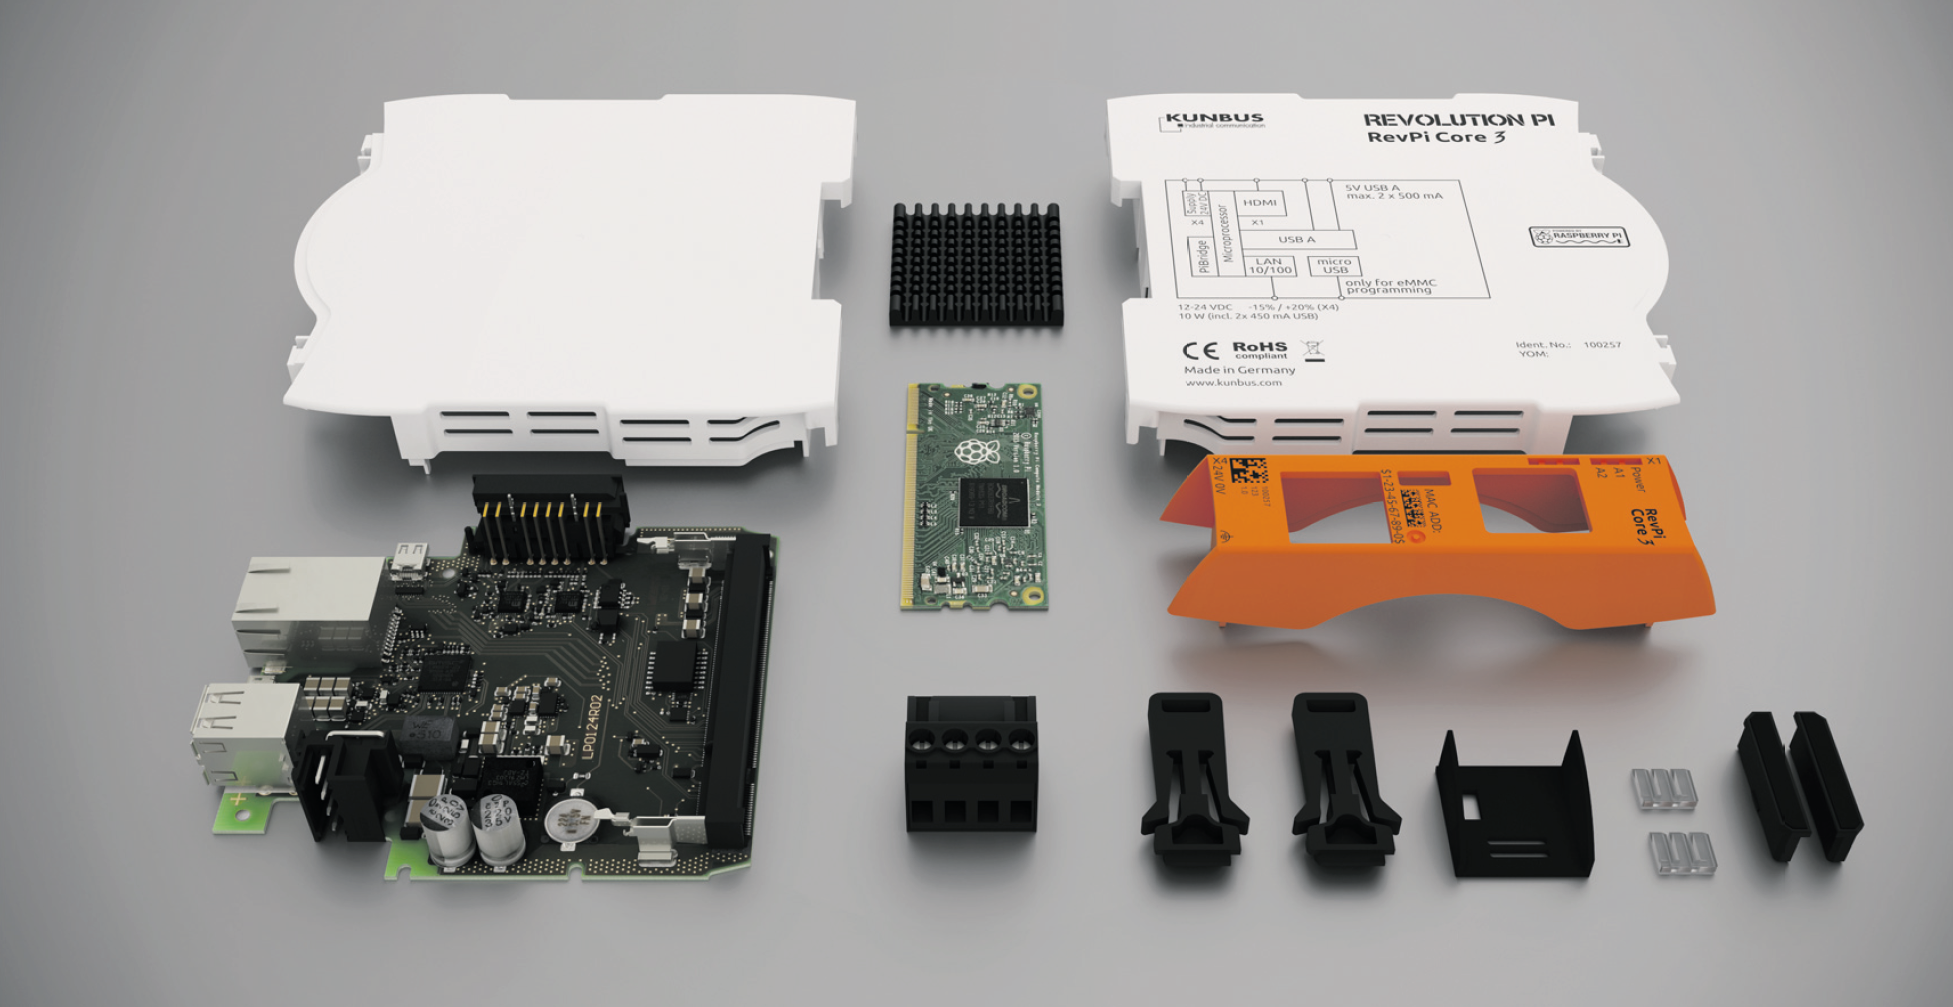
\includegraphics[width=0.85\textwidth]{doc/tex/images/revpi_teardown.png}
    \caption{Der RevPi Core 3 und seine Einzelkomponenten (Quelle: Kunbus)
      \label{fig:revpi-expl}}
\end{figure}

Spezifikationen des RevPi Core 3 \citep[Auswahl, vgl.][S. 1]{datasheet-revpi}:
\begin{itemize}
  \item{Prozessor: BCM2837}
  \item{Taktfrequenz 1,2 GHz}
  \item{Anzahl Prozessorkerne: 4}
  \item{Arbeitsspeicher: 1 GByte}
  \item{eMMC Flash Speicher: 4 GByte}
  \item{Betriebssystem: Angepasstes Raspbian mit RT-Patch}
  \item{RTC mit 24h Pufferung über wartungsfreien Kondensator}
  \item{Treiber / API: Kernel-Treiber schreibt zyklisch Prozessdaten in ein Prozessabbild, Zugriff auf Prozessabbild mittels ioctl-Anfragen oder über Linux-Dateisystem als API zu Fremdsoftware}
  \item{Kommunikationsanschlüsse: 2 x USB 2.0 A, 1 x Micro-USB, HDMI, Ethernet 10/100 Mbit/s}
  \item{Stromversorgung: min. 10,7 V, max. 28,8 V, maximal 10 Watt}
\end{itemize}

Kunbus stellt für den Revolution Pi ein auf Raspbian\footnote{Raspbian ist eine speziell 
für den Raspberry Pi angepasste Variante von Debian.} Stretch basierendes Betriebssystem bereit.
Verwendet wird der Kernel 4.9.76-rt60-v7+ in Verbindung mit dem SMP PREEMPT RT Patch.

\begin{figure}
    \centering
    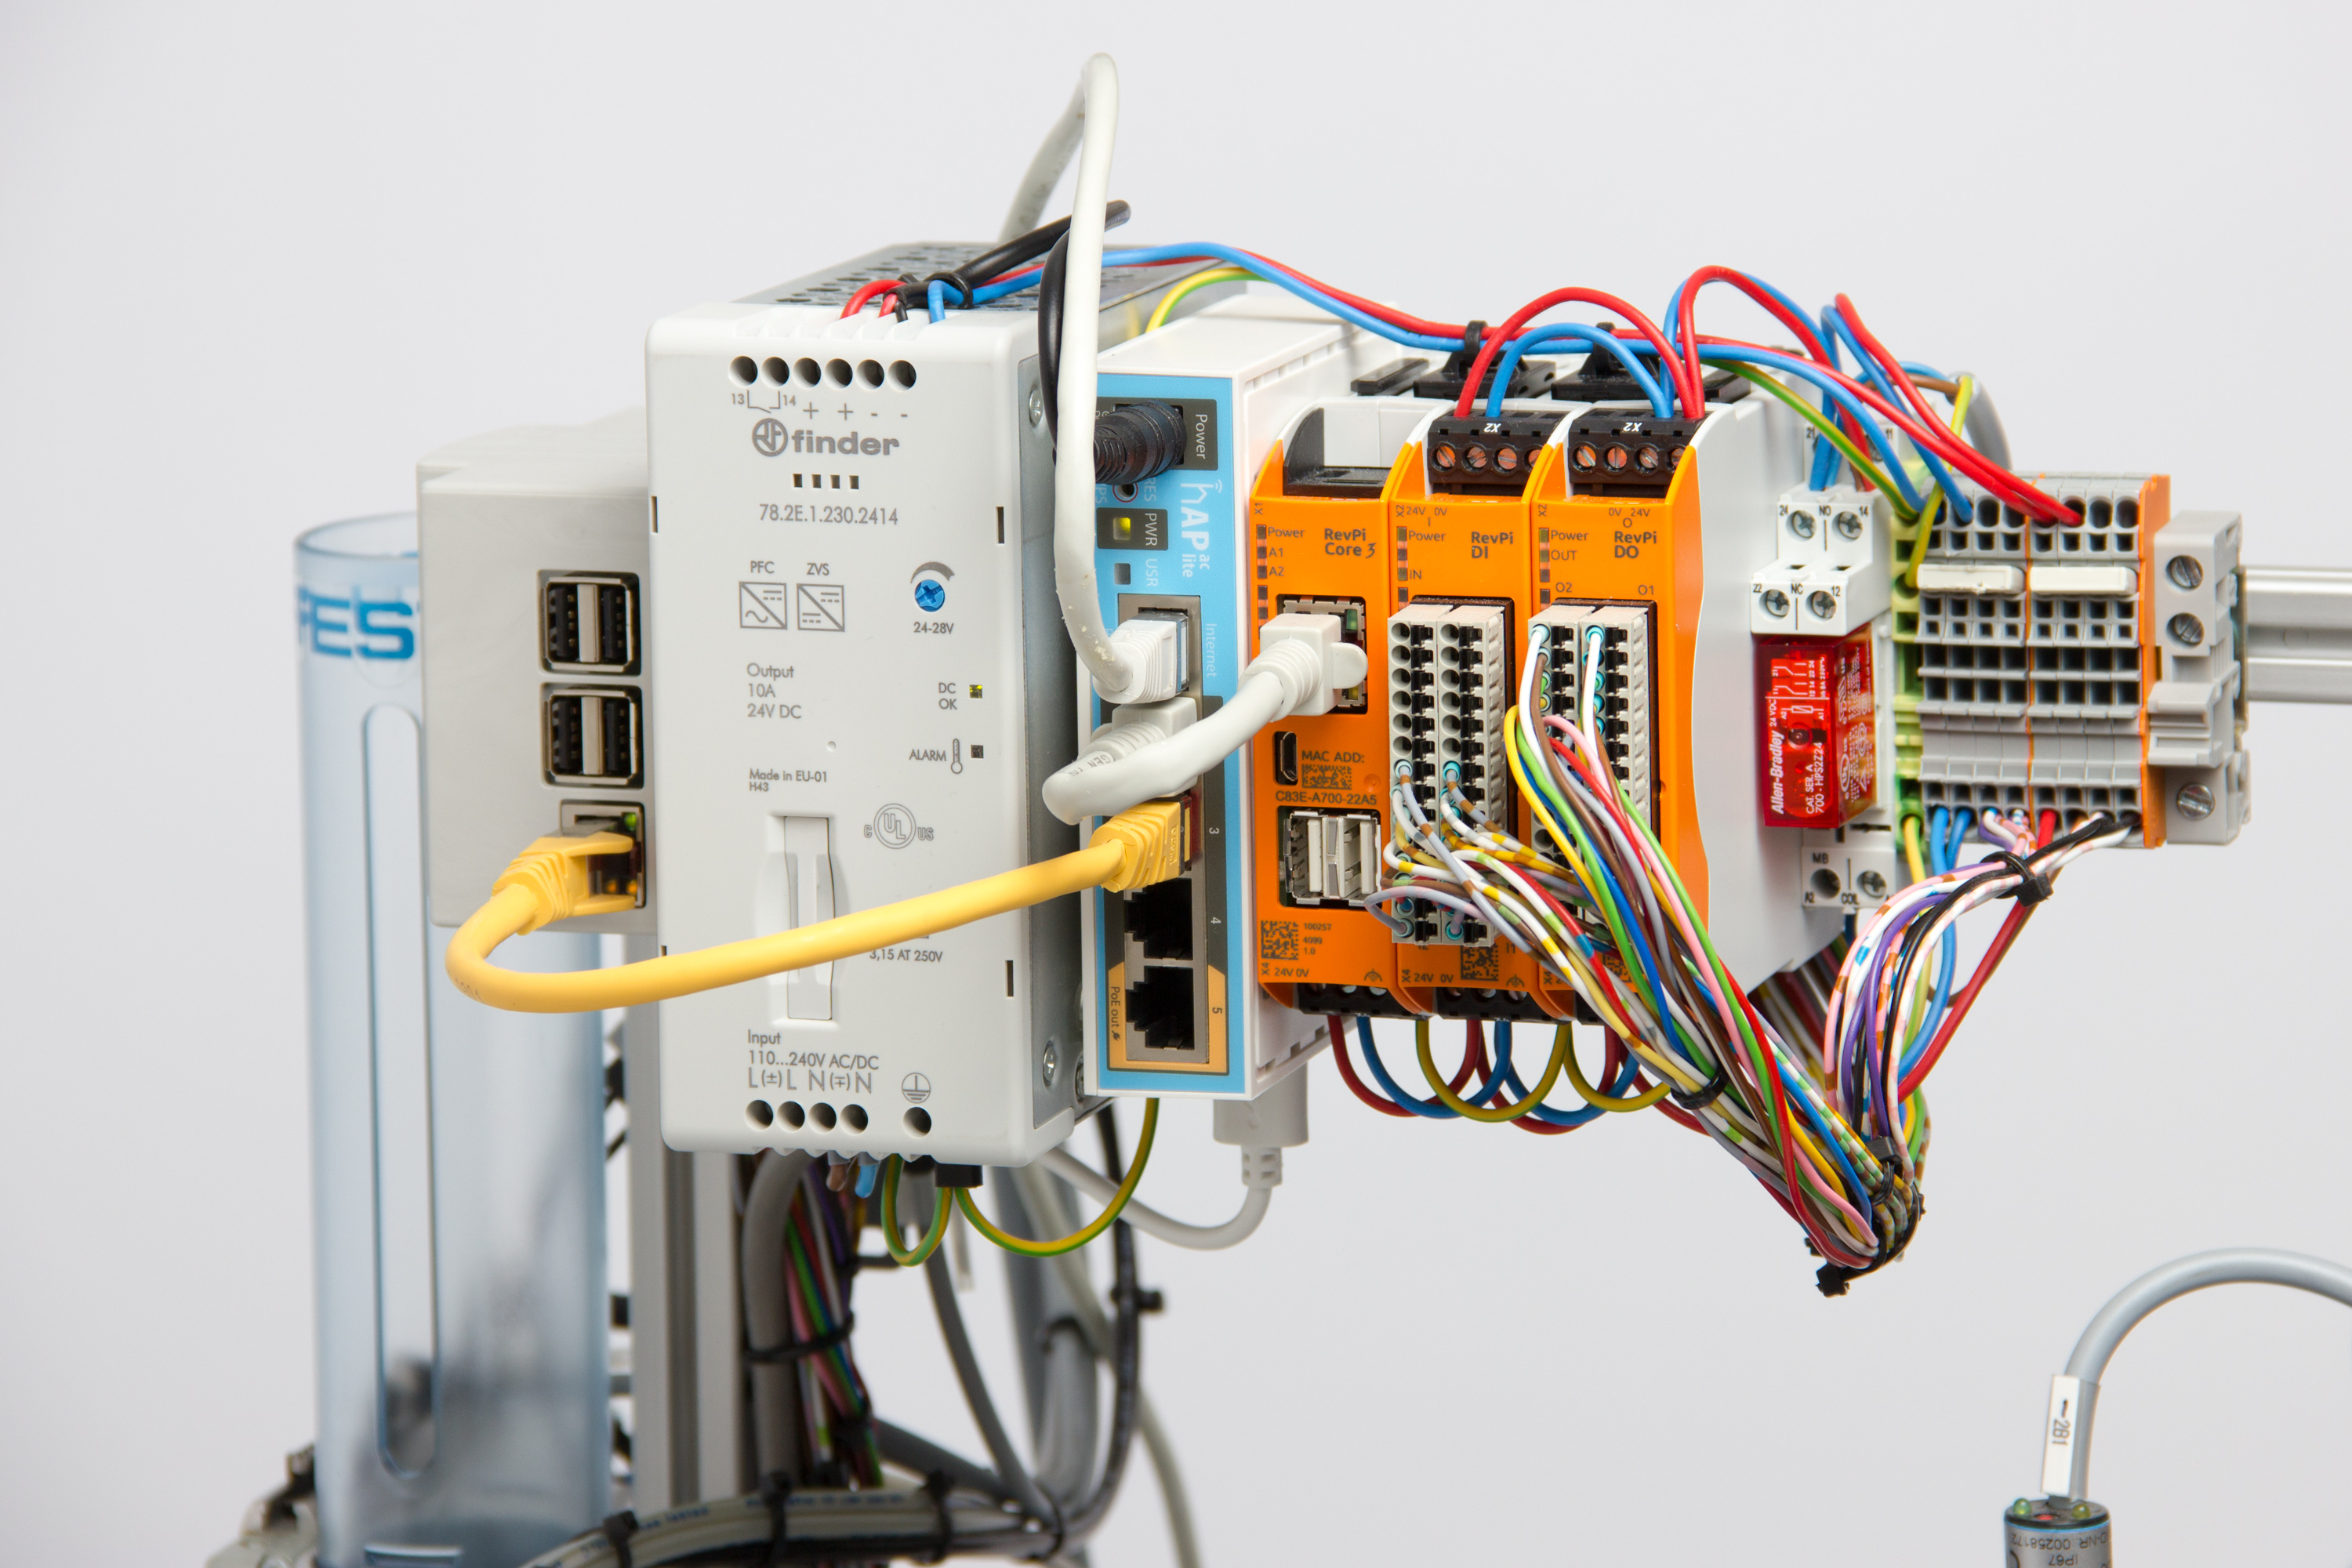
\includegraphics[trim={13cm 5cm 1cm 3cm}, clip, width=0.85\textwidth]{../photos/serverless_plc_img_8}
    \caption{Der Revolution Pi 3 mit digitalen IO-Modulen}
    \label{fig:rev-pi-io}
\end{figure}

Kunbus bietet neben dem sog. Core auch IO- und Gateway-Modulen zur Erweiterung der SPS an, siehe Bild~\ref{fig:rev-pi-io}.
Gateways dienen der Kommunikation mit externen Systemen oder Komponenten
über in der Automatisierungstechnik gängige Protokolle wie PROFIBUS oder EtherCAT. 
IO-Module erlauben die Überwachung und Steuerung von digitalen oder analogen Ein- und Ausgängen (IOs).

Kunbus deklariert die Hardware des Revolution Pi als Open-Source \citep[vgl.][S. 4]{flyer-revpi}. 
Die Schaltpläne des Revolution Pi, genauer die des RevPi Core 3 und der IO-Module, stehen auf der
Website\footnote{\label{downloads}\url{https://revolution.kunbus.com/tutorials/downloads/}} des Herstellers zum 
Download bereit. Eine Lizenz wird nicht angegeben.
Die Raspberry Pi Foundation stellt die Schaltpläne des Compute Modules des weiteren in ihrem Gitub-Repository 
zum Download bereit.

Sowohl die Raspberry Pi Foundation als auch die Kunbus GmbH pflegen aktiv ihre öffentlichen Repositories\footnote{\url{https://github.com/raspberrypi/} resp.~\url{https://github.com/RevolutionPi/}}
auf Github. 

% Kunbus konnte so einige Verbesserungen zum Linux Kernel 4.15 beitragen
% \footnote{siehe \url{https://revolution.kunbus.com/our-contribution-to-linux-4-15/}}.
% \todo{letzten Absatz evtl. weglassen? an sich nicht schlecht, passt aber irgendwie 
% nicht richtig zum Rest und stört den Lesefluss}

\subsubsection{Zugriff auf IO-Module%
        \label{sec:2-io}}
Der Zugriff auf die Ein- und Ausgänge der IO-Module erfolgt über einen RS485-Bus und einen in Form eines Kernel-Moduls bereitgestellten Treiber, genannt piControl. Der RS485-Bus ist über die serielle Schnittstelle des Compute Modules angebunden. 
piControl stellt ein Prozessabbild bereit, welches den physikalischen Zustand der Ein- und Ausgänge der IO-Module repräsentiert.
Das Prozessabbild wird, wie in der Automatisierungstechnik üblich, zyklisch aktualisiert. 
Die angestrebte Zykluszeit beträgt 5ms, kann jedoch je nach Anzahl der angeschlossenen Module auch größer sein. 
Kunbus garantiert bei drei IO-Modulen und zwei Gateway-Modulen eine Zykluszeit von 10 ms \citep[vgl.][]{web-revpi-dio}.
Die garantierte Zykluszeit ermöglicht die Umsetzung von Anwendungen mit harten Echtzeit-Anforderungen.

Fremdanwendungen können über eine Applikationsschnittstelle (API) auf das Prozessabbild zugreifen. 
Hierzu stellt das Kernel-Modul piControl sowohl \lstinline{seek}, \lstinline{read} und \lstinline{write} Methoden zur verfügung, wie auch die Möglichkeit mittels \lstinline{ioctl}-Anfragen gezielt auf einzelne Variablen des Prozessabbildes zuzugreifen.
In der englischsprachigen Wikipedia werden ioctl-Aufrufe wie folgt beschrieben:

\glqq{}The kernel is designed to be extensible, and may accept an extra module called a device driver which runs in kernel space and can directly address the device. An ioctl interface is a single system call by which userspace may communicate with device drivers. [...] The basic kernel can thus allow the userspace to access a device driver without knowing anything about the facilities supported by the device, and without needing an unmanageably large collection of system calls.

[...] ioctl calls provide a convenient way to bridge userspace code to kernel extensions. Kernel extensions can provide a location in the filesystem that can be opened by name, through which an arbitrary number of ioctl calls can be dispatched, allowing the extension to be programmed without adding system calls to the operating system.\grqq{}\citep[vgl.][]{web-wiki-ioctl}

Der Quellcode von piControl steht unter der GNU General Public License Version 2 (GNU GPLv2) und ist 
auf Github verfügbar\footnote{\url{https://github.com/RevolutionPi/piControl}}. Als Einstieg in die 
Entwicklung eigener Steuerungsprogramme liefert Kunbus das C-Programm piTest mit. Dieses verwendet 
piControl und erlaubt dem Nutzer über Kommandozeilen-Parameter die angeschlossenen IO-Module zu steuern.

\begin{figure}[h]
    \centering
    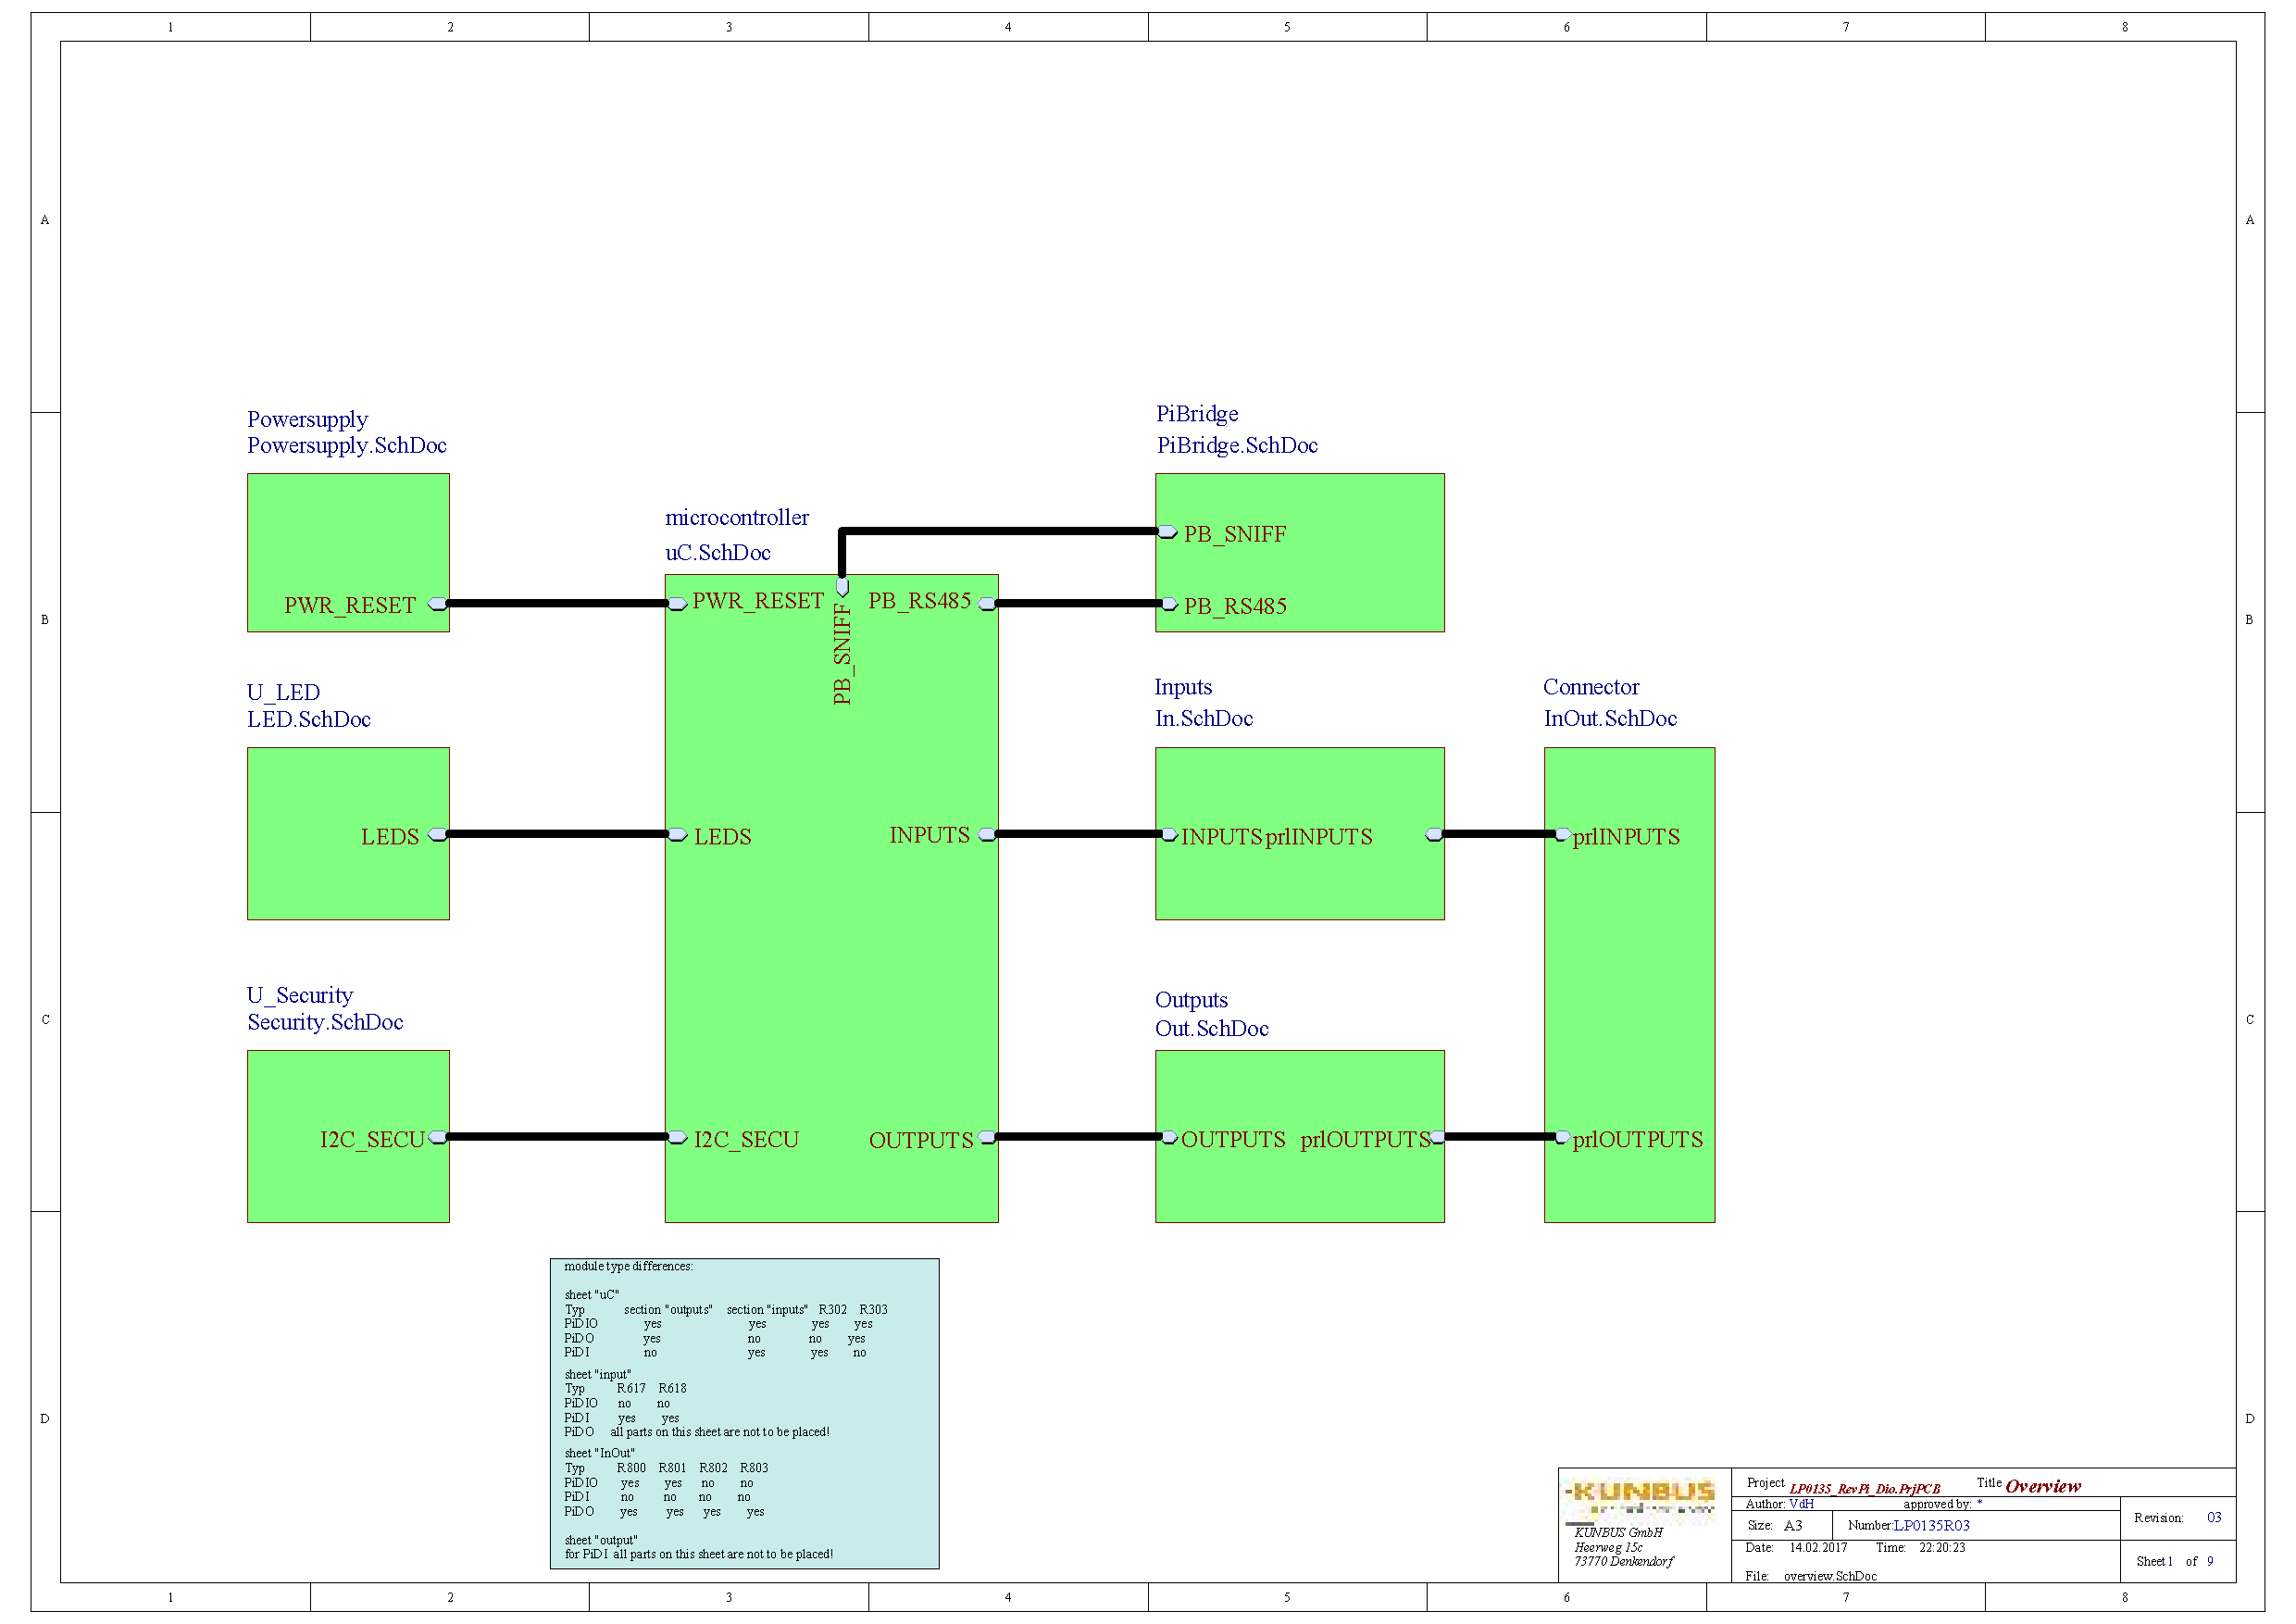
\includegraphics[trim={4cm 7cm 10.5cm 7.3cm}, clip, width=\textwidth]{literature/SchematicPrintsRevPi-DIO}
    \caption{Schematische Darstellung eines DIO-Moduls (Quelle: Kunbus\textsuperscript{\ref{downloads}})
      \label{fig:dio}}
\end{figure}

Jedes der IO-Module stellt ein eigenständiges eingebettetes System dar. Es verfügt
über einen Microcontroller, welcher die IOs bereitstellt und über einen RS485-Bus
mit dem Revolution Pi kommuniziert (siehe Bild~\ref{fig:dio}). 
Kunbus stellt exemplarisch den Quellcode eines DIO-Moduls unter der MIT Lizenz zur
Verfügung\footnote{\url{https://github.com/RevolutionPi/IODeviceExample}}. 


\subsection{Echtzeit und Multitasking unter Linux -- preemptRT und posix%
     \label{sec:2-echtzeit}}
     
Moderne Betriebssysteme realisieren Multitasking i.d.R.\,in Form des präemptiven Multitasking. 
Der Kernel verfügt über einen sog. Scheduler. Dieser priorisiert alle Prozesse und weist ihnen 
Rechenzeit in sog. Time Slots zu. Die Größe der Zeitfenster sowie die Ausführungsreihenfolge 
ist von der Priorität eines Prozesses abhängig. Besonders an einem präemptiven im Gegensatz zu einem kooperativen Scheduler ist dessen Fähigkeit, Tasks während ihrer Ausführung zu unterbrechen bzw. zu pausieren, wenn diese eine bestimmte Dauer überschreiten oder ein höher priorisierter Prozess (bspw. ausgelöst durch einen Interrupt oder durch eine inhärente Periodizität) Rechenleistung benötigt.

Eine Sonderform des präemptiven Multitasking ist das präemptible Multitasking. Hierbei werden auch Teile 
des Kernels als Threads durch den Scheduler ausgeführt. Dieser ist somit in der Lage, auch Prozesse des Kernels
zu unterbrechen, wenn andere Anwendungen Prozessorzeit oder Zugriff auf andere Systemressourcen benötigen
\citep[vgl.][]{web-wiki-praempt}.
     
Der Linux-Kernel implementiert unterschiedliche Präemptions-Modelle \citep[vgl.][/preemption\_models]{web-linuxwiki-basics}:

\begin{itemize}
  \item No Forced Preemption (server):
  Ausgelegt auf maximal möglichen Durchsatz, lediglich Interrupts und
  System-Call-Returns bewirken Präemption.

  \item Voluntary Kernel Preemption (Desktop):
  Neben den implizit bevorrechtigten Interrupts und System-Call-Returns gibt es
  in diesem Modell weitere Abschnitte des Kernels in welchen Preämption explizit
  gestattet ist.

  \item Preemptible Kernel (Low-Latency Desktop):
  In diesem Modell ist der gesamte Kernel, mit Ausnahme sog.~kritischer Abschnitte
  präemptible. Nach jedem kritischen Abschnitt gibt es einen impliziten Präemptions-Punkt.

  \item Preemptible Kernel (Basic RT):
  Dieses Modell ist dem zuvor genannten sehr ähnlich, hier sind jedoch alle Interrupt-Handler
  als eigenständige Threads ausgeführt.

  \item Fully Preemptible Kernel (RT):
  Wie auch bei den beiden zuvor genannten Modellen ist hier der gesamte Kernel
  präemtible. Die Anzahl und Dauer der nicht-präemtiblen kritischen Abschnitte
  ist auf ein notwendiges Minimum beschränkt. Alle Interrupt-Handler sind als
  eigenständige Threads ausgeführt, Spinlocks durch Sleeping-Spinlocks und Mutexe
  durch sog.~RT-Mutexe ersetzt.

\end{itemize}

Lediglich ein präemtibler Kernel kann hartes Echtzeit-Verhalten realisieren, 
da nur hier eine maximale Antwortzeit garantiert werden kann.
Viele Prozesse in der Automatisierungstechnik erfordern harte Echtzeit. 
Eine verspätete Antwort auf eine Anfrage, 
wie etwa das Signal eines Lagenendschalters oder eines Notausschalters kann hier nicht nur über
den Erfolg eines Prozesses, sondern auch über das Leben der daran beteiligten Mitarbeiter entscheiden.
Für weiterführende Erklärungen bzgl.\,Echtzeit, Mutexen und 
Spinlocks sei an dieser Stelle auf die Vorlesung verwiesen~\citep{script-peter}.


\subsubsection{preemptRT%
        \label{sec:2-preemptRT}}

Der Kernel des auf dem Revolution Pi installierten Raspbian mit PREEMP\_RT Patch fällt 
in die Kategorie des \glqq{}Fully Preemptible Kernels\grqq{} (siehe Abschnitt \ref{sec:2-echtzeit}).
Das zugrunde liegende Prinzip lässt sich wie folgt formulieren: Nur Code, welcher absolut nicht-präemtible sein darf, ist es
gestattet nicht-präemtible zu sein. Ziel ist folglich, die Menge des nicht-präemtiblen 
Codes im Linux-Kernel auf das absolut notwendige Minimum zu reduzieren.

Dies wird durch Verwendung folgender Mechanismen erreicht~\citep[vgl.][]{web-linuxwiki-details}:

\begin{itemize}
  \item Hochauflösende Timer
  \item Sleeping Spinlocks
  \item Threaded Interrupt Handlers
  \item rt\_mutex
  \item RCU
\end{itemize}

Diese Mechanismen sind bspw. im Linux-Wiki\footnote{siehe \url{https://wiki.linuxfoundation.org/realtime/documentation/technical_details}} ausführlich beschrieben.

\subsubsection{POSIX%
        \label{sec:2-posix}}
Das Portable Operating System Interface (POSIX) bezeichnet eine Sammlung von Standards, 
welche auf dem Unix-System basieren, jedoch nicht auf dieses beschränkt sind.

Der Wechsel zwischen verschiedenen Unix-Distributionen brachte oft Kompatibilitätsprobleme mit sich. 
Dieser Mangel an Portabilität erschwerte Benutzern und Entwicklern die Verwendung bzw. Bereitstellung 
von Software auf unterschiedlichen Systemen. 
Das Institut für Elektrotechnik und Elektronik (IEEE) begann 1984 mit der Entwicklung des Unix-Standards.
Sie entwickelten das, was heute als Single UNIX Specification bekannt ist und allgemein als POSIX bezeichnet wird~\citep[vgl.][]{web-debianwiki-posix}.
Das Konsortium \glqq{}The Open Group\grqq{} überwacht die weitere Entwicklung dieses Standards.
Ferner stellt es einen Teil der POSIX-Spezifikation frei zur Verfügung~\citep[vgl.][]{web-opengroup-posix}.

Die aktuelle Version POSIX.1-2017 ist verfügbar als IEEE Standard 1003.1-2017 sowie in Form der \glqq{}The Open Group Technical Standard Base Specifications\grqq{}, Ausgabe 7. POSIX.1-2017 definiert eine Standard-Betriebssystemschnittstelle und -umgebung, einschließlich eines Befehlsinterpreters (auch Shell genannt) und gängiger Dienstprogramme zur Unterstützung der Portabilität von Anwendungen auf Quellcode-Ebene. POSIX.1-2017 ist sowohl für Anwendungsentwickler als auch für Systemimplementierer gedacht und umfasst vier Hauptkomponenten \citep[vgl.][]{web-opengroup-overview}:
\begin{itemize}
    \item Basisdefinitionen:\\
          Allgemeine Begriffe, Konzepte und Schnittstellen einschließlich Hilfskonventionen und C-Headern
          
    \item Systemschnittstellen:\\
          Definitionen für Systemdienstfunktionen und Unterprogramme, C-spezifische Systemdienste, Portabilität
        
    \item Shell und Dienstprogramme:\\
          Definitionen für eine Schnittstelle zur Befehlsinterpretation von Diensten und gängige Hilfsprogramme
    
    \item Begründungen und Historie
\end{itemize}

Debian basiert auf Linux und verwendet den Linux-Kernel. Linux ist zu großen Teilen POSIX-kompatibel. Debian ist jedoch nicht POSIX-zertifiziert, da diese Zertifizierung mit hohen Kosten verbunden ist\citep[vgl.][Kapitel 4.4.]{web-debian-faq}.

Beide Kernkomponenten des in dieser Arbeit vorgestellten Projektes nutzen Komponenten von Linux, 
welche an den POSIX-Standard angelehnt sind: open62541 verwendet u.a.\,POSIX-Threads und
Mutexe~\citep[vgl.][pthread.h]{web-opengroup-pthread}, piControl nutzt POSIX-Semaphoren
\citep[vgl.][semaphore.h]{web-opengroup-semaphore}. 


\subsection{OPC-UA und open62541%
     \label{sec:2-opc}}
In diesem Abschnitt sollen Möglichkeiten des Datenaustausch zwischen Komponenten der
Automatisierungstechnik vorgestellt werden. OPC-UA stellt einen offenen, IP-basierten Kommunikationsstandard
für Sensoren und Steuerungen dar. open62541 ist eine freie Client- sowie Server-Implementierung dieses
Standards, geschrieben in C.


\subsubsection{OPC UA%
        \label{sec:2-opcua}}

Open Platform Communications (OPC) ist eine Familie von Standards zur herstellerunabhängigen
Kommunikation von Maschinen (M2M) in der Automatisierungstechnik. Die sog. OPC Task Force, zu deren
Mitgliedern verschiedene etablierte Firmen der Automatisierungsindustrie gehören, veröffentlichte
die OPC Specification Version 1.0 im August 1996.
Motiviert ist dieser offene Standard durch die Erkenntniss, dass die Anpassung der
zahlreichen Herstellerstandards an individuelle Infrastrukturen und Anlagen einen
großen Mehraufwand verursachen.
Die Wikipedia beschreibt das Anwendungsgebiet für OPC wie folgt \citep[vgl.][]{web-wiki-opc}:

\glqq{}OPC wird dort eingesetzt, wo Sensoren, Regler und Steuerungen verschiedener Hersteller
ein gemeinsames Netzwerk bilden. Ohne OPC benötigten zwei Geräte zum Datenaustausch
genaue Kenntnis über die Kommunikationsmöglichkeiten des Gegenübers. Erweiterungen
und Austausch gestalten sich entsprechend schwierig. Mit OPC genügt es, für jedes
Gerät genau einmal einen OPC-konformen Treiber zu schreiben. Idealerweise wird
dieser bereits vom Hersteller zur Verfügung gestellt. Ein OPC-Treiber lässt sich
ohne großen Anpassungsaufwand in beliebig große Steuer- und Überwachungssysteme
integrieren.

OPC unterteilt sich in verschiedene Unterstandards, die für den jeweiligen Anwendungsfall
unabhängig voneinander implementiert werden können. OPC lässt sich damit verwenden
für Echtzeitdaten (Überwachung), Datenarchivierung, Alarm-Meldungen und neuerdings
auch direkt zur Steuerung (Befehlsübermittlung).\grqq{}

OPC basiert in der ursprünglichen Spezifikation (auch als OPC DA bezeichnet) auf Microsofts DCOM-Spezifikation.
DCOM macht Funktionen und Objekte einer Anwendung anderen Anwendungen im Netzwerk
zugänglich. Der OPC-Standard definiert entsprechende DCOM-Objekte um mit anderen
OPC-Anwendungen Daten austauschen zu können. Die Verwendung von DCOM bindet Anwender
jedoch an Betriebssysteme von Microsoft. 

\begin{figure}
    \centering
    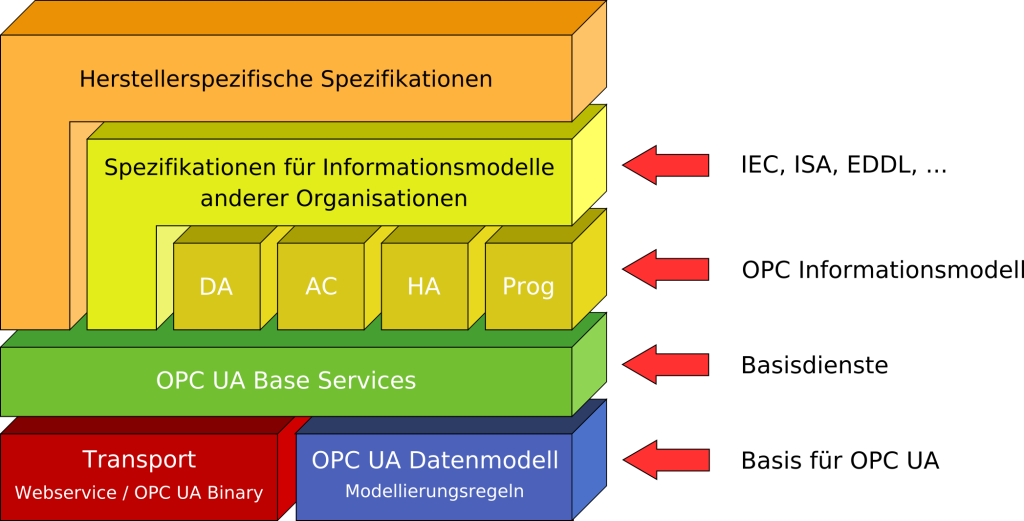
\includegraphics[width=0.85\textwidth]{images/UA_Architecture_1024.png}
    \caption{Die OPC Unified Architecture. Grafik von Gerhard Gappmeier - ascolab GmbH, CC BY-SA 3.0}
    \label{fig:opc-unified-architecture}
\end{figure}
% Evtl Grafik: Von Gerhard Gappmeier - ascolab GmbH, CC BY-SA 3.0, https://de.wikipedia.org/w/index.php?curid=1892069

Die ursprüngliche OPC Spezifikation wurde 2006 durch die Entwicklung der 
OPC Unified Architecture (OPC UA) überholt. 
Diese zeichnet sich durch eine Service-orientierte Architektur (SOA) aus, deren Struktur
aus mehreren Schichten besteht, siehe Abbilung~\ref{fig:opc-unified-architecture}. 
Über der untersten Schicht, dem Betriebssystem des Servers, verbindet eine Portabilitäts-Schicht 
den sog.\, UA ANSI C Stack mit einer API. Diese API kann bspw.\,in C++ geschrieben sein, 
und erlaubt die Anbindung der obersten Schicht, der Anwendungsschicht~\citep[vgl.][]{web-spec-opc}.
OPC UA setzt auf einem eigenen Kommunikationsstack auf; die Verwendung von DCOM
und damit die Bindung an Microsoft wurden aufgelöst.

Neben Architektur und Kommunikationsschnittstellen wird in der OPC Spezifikation auch ein 
Informationsmodell definiert. Die deutschsprachige Wikipedia beschreibt dieses wie folgt: 

\glqq{}Das OPC[-UA]-Informationsmodell ist nicht mehr nur eine Hierarchie aus Ordnern, Items
und Properties. Es ist ein sogenanntes Full-Mesh-Network aus Nodes, mit dem neben
den Nutzdaten eines Nodes auch Meta- und Diagnoseinformationen repräsentiert werden. [...]
Ein Node ähnelt einem Objekt aus der objektorientierten Programmierung. Ein Node
kann Attribute besitzen, die gelesen werden können. Es ist möglich Methoden zu definieren und aufzurufen. [...]
Weiterhin werden Events unterstützt, die versendet werden können
(AE (Alarms \& Events), DA DataChange), um bestimmte Informationen zwischen Geräten
auszutauschen. Ein Event besitzt unter anderem einen Empfangszeitpunkt, eine Nachricht
und einen Schweregrad. Die o.\,g. Nodes werden sowohl für die Nutzdaten als auch
alle anderen Arten von Metadaten verwendet. Der damit modellierte OPC-Adressraum
beinhaltet nun auch ein Typmodell, mit dem sämtliche Datentypen spezifiziert werden.\grqq{}


\subsubsection{open62541%
        \label{sec:2-open62541}}
open62541 ist eine offene und freie Implementierung von OPC UA. 
Die in C geschriebene Bibliothek stellt eine beständig zunehmende Anzahl der im OPC UA Standard definierten
Funktionen bereit. Sie kann sowohl zur Erstellung von OPC-Servern als auch von -Clients
genutzt werden. Ergänzend zu der unter der Mozilla Public License v2.0 lizensierten
Bibliothek stellt das open62541 Projekt auch Beispielprogramme unter einer CC0 Lizenz
zur Verfügung.
Zu den Unterstützern des Projektes zählen u.a.\, die RWTH Aachen, das Frauenhofer IOSB sowie die TU Dresden.

Die Bibliothek eignet sich auch für die Entwicklung auf eingebetteten Systemen und
Microcontrollern. Die Größe einer Server-Binary kann weniger als 100kB betragen.

Folgende Auswahl an Eigenschaften und Funktionen zeichnet die in dieser Arbeit verwendete
Version 0.3 von open62541 aus:
\begin{itemize}
  \item Kommunikationionsstack
  \begin{itemize}
      \item OPC UA Binär-Protokoll (HTTP oder SOAP werden gegenwärtig nicht unterstützt)
      \item Austauschbare Netzwerk-Schicht, welche die Verwendung eigener Netzwerk-APIs
      erlaubt.
      \item Verschlüsselte Kommunikationion
      \item Asynchrone Dienst-Anfragen im Client
  \end{itemize}
  \item Informationsmodell
  \begin{itemize}
    \item Unterstützung aller OPC UA Node-Typen, inkl.~Methoden
    \item Hinzufügen und Entfernen von Nodes und Referenzen zur Laufzeit.
    \item Vererbung und Instanziierung von Objekt- und Variablentypen
    \item Zugriffskontrolle auch für einzelne Nodes
  \end{itemize}
  \item Subscriptions
  \begin{itemize}
    \item Erlaubt die Überwachung (subscriptions / monitoreditems)
    \item Sehr geringer Ressourcenbedarf pro überwachtem Wert
  \end{itemize}
  \item Code-Generierung auf XML-Basis
  \begin{itemize}
    \item Erlaubt die Erstellung von Datentypen
    \item Erlaubt die Generierung des serverseitigen Informationsmodells
  \end{itemize}
\end{itemize}

Weiterführende Informationen und Code-Beispiele bietet die ausführliche Dokumentation des Projektes~\citep[siehe]{web-open62541} sowie der kommentierte Quelltext.

% % % Imports nur für Referenzenauflösung während des Schreibens! Vorm Kompilieren auskommentieren!
% \bibliography{0_hauptdatei}
% \input{1_einleitung}
% \input{2_grundlagen}
% \input{3_konzeption}
% \input{4_implementierung}
% \input{5_tests}
% \input{6_zusammenfassung}
% \input{anhang}
% % Ende Imports

\section{Systemkonzept%
  \label{sec:3-konzeption}}
Auf Basis der in Abschnitt [...] vorgestellten Möglichkeiten folgt nun die Ausarbeitung eines Konzepts.

\subsection{Anbindung der IO an den OPC-Server%
     \label{sec:3-anbindung}}

\subsection{Integration des OPC-Servers in das System%
     \label{sec:3-integration}}

% % % Imports nur für Referenzenauflösung während des Schreibens! Vorm Kompilieren auskommentieren!
% \bibliography{0_hauptdatei}
% \input{1_einleitung}
% \input{2_grundlagen}
% \input{3_konzeption}
% \input{4_implementierung}
% \input{5_tests}
% \input{6_zusammenfassung}
% \input{anhang}
% % Ende Imports

\section{Implementierung%
  \label{sec:4-implementierung}}
Das folgende Kapitel stellt in Auszügen die Implementierung des OPC-Servers sowie die Anbindung an die IO-Module
der SPS dar. Der Schwerpunkt liegt hierbei auf der Funktionsweise des piControl-Treibers und dessen Integration in das Projekt. Abschnitt~\ref{sec:4-picontrol} erklärt die zum Schreibens eines Bits verwendeten Funktionsaufrufe.
Zuvor soll jedoch in Abschnitt~\ref{sec:4-open62541} der Teil des OPC-Servers vorgestellt werden, welcher auf besagten Treiber zugreift. 

\subsection{Implementierung des OPC-Servers%
     \label{sec:4-open62541}}
Wie im vorangegangenen Abschnitt~\ref{sec:3-integration} begründet, soll die Verknüpfung zwischen dem Prozessabbild der SPS und den auf dem OPC-Server bereitgestellten Werten über sog.\,Datenquellen erfolgen. Hierzu ist zunächst eine Callback-Methode zu implementieren, welche bei einem Lese- oder Schreibzugriff auf eine Variable aufgerufen wird. Die Verknüpfung zwischen Callback-Methode und Variable muss manuell erfolgen.

\begin{lstlisting}[language={c},firstnumber=237,caption={Auszug der Methode \lstinline{linkDataSourceVariable} in \lstinline{variables.c}\label{lst:4-linkDataSourceVariable}}]
extern UA_StatusCode
 linkDataSourceVariable(UA_Server *server, UA_NodeId nodeId) {
     bool readonly = false;
     UA_DataSource dataSourceVariable;
     UA_StatusCode rc; |>\setcounter{lstnumber}{254}<|

     dataSourceVariable.read = readDataSourceVariable;
     if (!readonly)
        dataSourceVariable.write = writeDataSourceVariable;
     else
        dataSourceVariable.write = writeReadonlyDataSourceVariable;

     return UA_Server_setVariableNode_dataSource(server, nodeId, dataSourceVariable);
 }
\end{lstlisting}

\begin{figure}[h]
    \centering
    \includegraphics[width=0.42\textwidth]{doc/img/OPC_RevPiDO.pdf}
    \caption{Auszug des verwendeten Nodesets, hier Digitalausgang 1 des Versuchsaufbaus
      \label{fig:opc-do}}
\end{figure}

Die in Listing~\ref{lst:4-linkDataSourceVariable} abgebildete Methode \lstinline{linkDataSourceVariable()} erzeugt ein Struct vom Typ \lstinline{UA_DataSource}. In diesem werden dem Lesen und Schreiben einer OPC-Variablen entsprechende Callback-Methoden zugewiesen. Die Verknüpfung einer OPC-Variable, genauer ihrer NodeId, mit der zuvor definierten Datenquelle erfolgt über die von open62541 bereitgestellte Methode \lstinline{UA_Server_setVariableNode_dataSource()}. Vor dem Lesen und nach dem Schreiben dieser Variable werden von nun an die entsprechenden Callbacks aufgerufen.
     
\begin{lstlisting}[language={c},firstnumber=168,caption={Auszug des Callbacks \lstinline{writeDataSourceVariable} in \lstinline{variables.c}\label{lst:4-writeDataSourceVariable}}]  
extern UA_StatusCode
 writeDataSourceVariable(UA_Server *server,
            const UA_NodeId *sessionId, void *sessionContext,
            const UA_NodeId *nodeId, void *nodeContext,
            const UA_NumericRange *range, const UA_DataValue *dataValue) {

    UA_StatusCode retval  = UA_STATUSCODE_GOOD;
    UA_NodeId *nameNodeId = UA_malloc(sizeof(UA_NodeId));
    UA_QualifiedName nameQN = UA_QUALIFIEDNAME(1, "Name");
    UA_Variant nameVar;
    UA_Boolean bit;

    retval |= findSiblingByBrowsename(server, nodeId, &nameQN, nameNodeId);
    retval |= UA_Server_readValue(server, *nameNodeId, &nameVar);
    retval |= UA_Boolean_copy(dataValue->value.data, &bit);

    |>\tikzmarkin[set border color=martinired]{writeIO}<|PI_writeSingleIO(String_fromUA_String(nameVar.data), &bit, false);                                                 |>\tikzmarkend{writeIO}<|

    free(nameNodeId);
    return retval;
 }
\end{lstlisting}

Listing~\ref{lst:4-writeDataSourceVariable} zeigt die Callback-Methode, welche nach dem Schreiben einer Variablen auf dem OPC-Server aufgerufen wird.
Dieser Methode wird neben der NodeId der mit ihr verknüpften Variablen auch der Wert dieser in Form eines Zeigers auf ein Struct vom Typ \lstinline{UA_DataValue} übergeben.

Die Gestaltung des hier verwendeten Nodesets sieht vor, dass in einer OPC-Variablen \lstinline{"Name"} der Bezeichner des zu schreibenden Digitalausgangs hinterlegt ist, siehe Abbildung~\ref{fig:opc-do}. Dies erlaubt eine Rekonfiguration der Ein- und Ausgänge der SPS ohne Änderungen im Programmcode des OPC-Servers vornehmen zu müssen.
Es ist daher erforderlich, nach jedem Schreiben einer mit einem Digitalausgang verknüpften Variablen, hier \lstinline{"Value"}, dessen Bezeichner \lstinline{"Name"} abzufragen. 
Dies geschieht in den Zeilen 180 und 181.
Anschließend wird dieser Bezeichner sowie der zu schreibende Wert der Methode \lstinline{PI_writeSingleIO()} übergeben, welche wiederum die Interaktion mit piControl übernimmt (vgl. Abschnitt \ref{sec:4-picontrol}).
 
\subsection{Integration von piControl%
     \label{sec:4-picontrol}}
In Abschnitt~\ref{sec:2-io} wurde die Anbindung der IO-Module des Revolution Pi sowie die Funktionsweise von piControl aus Anwendersicht beschrieben. Die verfügbare Literatur beschränkt sich auch auf lediglich diese Sicht; eine weiterführende Dokumentation für Entwickler gibt es, neben der in Abschnitt~\ref{sec:3-anbindung} vorgestellten Manpage, nicht. 
In diesem Abschnitt soll daher der Quellcode von piControl sowie dessen Verwendung im Projekt genauer betrachtet werden.
Hierzu wird exemplarisch die in Abschnitt~\ref{sec:4-open62541} eingeführte Methode \lstinline{PI_writeSingleIO()} untersucht.
Diese Methode ermöglicht das Setzen eines einzelnen Bits im Prozessabbild der SPS, und damit das Schalten eines digitalen Ausgangs auf einem IO-Modul.
Die äquivalente Methode \lstinline{int piControlGetBitValue(SPIValue *pSpiValue)} zum Lesen eines Bits bzw. Eingangs funktioniert analog und soll daher an dieser Stelle nicht dediziert erörtert werden.

\begin{lstlisting}[language={c},firstnumber=97,
                   caption={Setzen eines phsikalischen, digitalen Ausgangs in \lstinline{revpi.c}
                   \label{lst:4-PI_writeSingleIO}}]
extern void PI_writeSingleIO(char *pszVariableName, bool *bit, bool verbose)
{
	int rc;
	SPIVariable sPiVariable;
	SPIValue sPIValue;

	strncpy(sPiVariable.strVarName, pszVariableName, sizeof(sPiVariable.strVarName));
	rc = piControlGetVariableInfo(&sPiVariable);
	if (rc < 0) {
		printf("Cannot find variable '%s'\n", pszVariableName);
		return;
	}

		sPIValue.i16uAddress = sPiVariable.i16uAddress;
		sPIValue.i8uBit = sPiVariable.i8uBit;
		sPIValue.i8uValue = *bit;
		rc = |>\tikzmarkin[set border color=martinired]{setBitValue}<|piControlSetBitValue(&sPIValue)|>\tikzmarkend{setBitValue}<|;
		if (rc < 0)
			printf("Set bit error %s\n", getWriteError(rc));
		else if (verbose)
			printf("Set bit %d on byte at offset %d. Value %d\n", sPIValue.i8uBit, sPIValue.i16uAddress,
			       sPIValue.i8uValue);
}
\end{lstlisting}

Der Programmcode in Listing~\ref{lst:4-PI_writeSingleIO} ist Teil des implementierten OPC-Servers. In diesem wird auf zwei Funktionen des piControl-Treibers zugegriffen. 
Beiden Methoden wird als Argument ein Zeiger auf ein Struct vom Typ \lstinline{SPIValue} übergeben. Der im Struct abgelegte Name wird mittels \lstinline{piControlGetVariableInfo(&sPIValue)} zu einer Adresse im Prozessabbild aufgelöst. Diese wird in \lstinline{sPIValue.i16uAdress} gespeichert. Der Wert der Variablen wird anschließend mittels \lstinline{piControlSetBitValue(&sPIValue)} an dieser Adresse in das Prozessabbild geschrieben.

\begin{lstlisting}[language={c},firstnumber=309,caption={Methode \lstinline{piControlSetBitValue} in \lstinline{piControlIf.c}\label{lst:4-piControlSetBitValue}}]
int |>\tikzmarkin[set border color=martiniblue]{setBitValueFcn}<|piControlSetBitValue(SPIValue *pSpiValue)|>\tikzmarkend{setBitValueFcn}<|
{
    piControlOpen();

    if (PiControlHandle_g < 0)
	    return -ENODEV;

    pSpiValue->i16uAddress += pSpiValue->i8uBit / 8;
    pSpiValue->i8uBit %= 8;

    if (|>\tikzmarkin[set border color=martinired]{ioctl}<|ioctl(PiControlHandle_g, KB_SET_VALUE, pSpiValue)|>\tikzmarkend{ioctl}<| < 0)
	    return errno;

    return 0;
}
\end{lstlisting}

Die in Listing~\ref{lst:4-piControlSetBitValue} dargestellte Methode \lstinline{piControlSetBitValue} ist lediglich eine Hüllfunktion (häufig auch als Wrapper-Funktion bezeichnet) für einen Aufruf des \lstinline{ioctl} Kernel-Moduls.
Folgende Parameter werden übergeben:
\lstinline{PiControlHandle_g} ist die Referenz auf die Geräte-Datei des piControl-Treibers. \lstinline{KB_SET_VALUE} ist das ioctl-Kommando zum Schreiben eines Bits in das Prozessabbild. Der Zeiger \lstinline{pSpiValue} verweist auf ein Struct des bereits vorgestellten Typs \lstinline{SPIValue}.

\begin{lstlisting}[language={c},firstnumber=80,caption={Methode \lstinline{piControlOpen} in \lstinline{piControlIf.c}\label{lst:4-piControlOpen}}]
void piControlOpen(void)
{
    /* open handle if needed */
    if (PiControlHandle_g < 0)
    {
	    |>\tikzmarkin[set border color=martiniblue]{PiControlHandle}<|PiControlHandle_g = open(PICONTROL_DEVICE, O_RDWR)|>\tikzmarkend{PiControlHandle}<|;
    }
}
\end{lstlisting}

Die in Listing~\ref{lst:4-piControlOpen} dargestellte Methode öffnet, sofern nicht bereits geschehen, die Geräte-Datei. Das Macro \lstinline{PICONTROL_DEVICE} verweist hierbei auf \lstinline{/dev/piControl0}.

\begin{lstlisting}[language={c},firstnumber=721,caption={Methode \lstinline{piControlIoctl} in \lstinline{piControlMain.c}\label{lst:4-piControlIoctl}}]
static long |>\tikzmarkin[set border color=martiniblue, below offset=0.9em]{piControlIoctl}<|piControlIoctl(struct file *file, unsigned int prg_nr, 
                           unsigned long usr_addr)                                      |>\tikzmarkend{piControlIoctl}<|
{
  int status = -EFAULT;
  tpiControlInst *priv;
  int timeout = 10000;	// ms

  if (prg_nr != KB_CONFIG_SEND && prg_nr != KB_CONFIG_START && !isRunning()) {
  	return -EAGAIN;
  }

  priv = (tpiControlInst *) file->private_data;

  if (prg_nr != KB_GET_LAST_MESSAGE) {
  	// clear old message
  	priv->pcErrorMessage[0] = 0;
  }

  switch (prg_nr) {|>\setcounter{lstnumber}{864}<|

    case |>\tikzmarkin[set border color=martiniblue]{KB_SET_VALUE}<|KB_SET_VALUE:|>\tikzmarkend{KB_SET_VALUE}<|
  		{
  			SPIValue *pValue = (SPIValue *) usr_addr;

  			if (!isRunning())
  				return -EFAULT;

  			if (pValue->i16uAddress >= KB_PI_LEN) {
  				status = -EFAULT;
  			} else {
  				INT8U i8uValue_l;
  				my_rt_mutex_lock(&piDev_g.lockPI);
  				i8uValue_l = piDev_g.ai8uPI[pValue->i16uAddress];

  				if (pValue->i8uBit >= 8) {
  					i8uValue_l = pValue->i8uValue;
  				} else {
  					if (pValue->i8uValue)
  						i8uValue_l |= (1 << pValue->i8uBit);
  					else
  						i8uValue_l &= ~(1 << pValue->i8uBit);
  				}

  				|>\tikzmarkin[set border color=martinired]{i8uValue}<|piDev_g.ai8uPI[pValue->i16uAddress] = i8uValue_l;|>\tikzmarkend{i8uValue}<|
  				rt_mutex_unlock(&piDev_g.lockPI);

  #ifdef VERBOSE
  				pr_info("piControlIoctl Addr=%u, bit=%u: %02x %02x\n", pValue->i16uAddress, pValue->i8uBit, pValue->i8uValue, i8uValue_l);
  #endif

  				status = 0;
  			}
  		}
  		break; |>\setcounter{lstnumber}{1314}<|

    default:
      pr_err("Invalid Ioctl");
      return (-EINVAL);
      break;

    }

    return status;
  }
\end{lstlisting}

Listing~\ref{lst:4-piControlIoctl} zeigt in Auszügen die ioctl-Methode des piControl Kernel-Treibers. Diese bekommt folgende Argumente übergeben: \lstinline{struct file *file} enthält den Verweis auf die Geräte-Datei, hier \lstinline{/dev/piControl0}. Der Wert von \lstinline{unsigned int prg_nr} beschreibt die Anfrage an den Treiber, in diesem Fall \lstinline{KB_SET_VALUE}. Das Argument \lstinline{unsigned long usr_addr} enthält einen typ-agnostischen Pointer. Dieser verweist auf einen Speicherbereich, in welchem die zur Bearbeitung der Anfrage notwendigen Daten abgelegt sind. Hier können auch vom Treiber empfangene Daten dem Anwendungsprogramm bereitgestellt werden. 

Die switch-case-Anweisung führt die über das Argument \lstinline{prg_nr} spezifizierte Aktion aus. Hier betrachten wir \lstinline{KB_SET_VALUE}:
Zunächst wird in Zeile 868 der übergebene Zeiger \lstinline{usr_addr} mittels explizitem Typecast zu einem Zeiger des Typs \lstinline{SPIValue *} konvertiert. Da dieser auf Daten im Userspace verweist, ist beim Zugriff durch den Kernel-Treiber besondere Vorsicht geboten.
In Zeile 877 wird mittels Mutex das Prozessabbild \lstinline{piDev_g} für den Zugriff durch andere Threads oder Prozesse gesperrt.
\lstinline{my_rt_mutex_lock} verweist hierbei auf die Funktion \lstinline{rt_mutex_lock} aus \lstinline{linux/sched.h}\footnote{Offenbar wurde hier auch eine alternative Implementierung vorgesehen, siehe revpi\_common.h}

In Zeile 889 wird das Byte \lstinline{i8uValue_l}, welches den zu schreibenden Wert enthält in das Prozessabbild übertragen. Anschließend wird die Mutex auf \lstinline{piDev_g} wieder entsperrt.
\newpage

\begin{lstlisting}[language={c},firstnumber=62,caption={Auszug des Struct \lstinline{spiControlDev} in \lstinline{piControlMain.h}\label{lst:4-spiControlDev}}]
|>\tikzmarkin[set border color=martiniblue]{spiControlDev}<|typedef struct spiControlDev|>\tikzmarkend{spiControlDev}<| {
	// device driver stuff
	int init_step;
	enum revpi_machine machine_type;
	void *machine;
	struct cdev cdev;	// Char device structure
	struct device *dev;
	struct thermal_zone_device *thermal_zone;

	|>\tikzmarkin[set border color=martiniblue]{processImage}<|// process image stuff
	INT8U ai8uPI[KB_PI_LEN];
	INT8U ai8uPIDefault|>\tikzmarkin[set border color=martinired]{KB_PI_LEN_0}<|[KB_PI_LEN]|>\tikzmarkend{KB_PI_LEN_0}<|;
	struct rt_mutex lockPI;        |>\tikzmarkend{processImage}<|
	bool stopIO;
	piDevices *devs; |>\setcounter{lstnumber}{94}<|
} tpiControlDev;
\end{lstlisting}

Das Prozessabbild ist als Byte-Array der Länge \lstinline{KB_PI_LEN} in Listing~\ref{lst:4-spiControlDev} definiert. Konfigurationsparameter wie \lstinline{KB_PI_LEN} oder die Zykluszeit für den Datenaustausch zwischen SPS und IO-Modulen sind im folgenden Listing~\ref{lst:4-process} definiert.

\begin{lstlisting}[language={c},firstnumber=119,caption={Konfigurationsparameter des Prozessabbildes in project.h\label{lst:4-process}}]
#define INTERVAL_PI_GATE (5*1000*1000)  // 5 ms piGateCommunication |>\setcounter{lstnumber}{128}<|

#define INTERVAL_IO_COM (5*1000*1000)  // 5 ms piIoComm |>\setcounter{lstnumber}{132}<|

#define KB_PD_LEN       512
|>\tikzmarkin[set border color=martiniblue]{KB_PI_LEN_1}<|#define KB_PI_LEN       4096|>\tikzmarkend{KB_PI_LEN_1}<|
\end{lstlisting}

Das zu setzende Bit wurde zu diesem Zeitpunkt erfolgreich in das Prozessabbild der SPS geschrieben.
Es stellt sich die Frage, wie dieses nun an das IO-Modul kommuniziert wird.
Die Kommunikation mit allen angebundenen Modulen ist ebenfalls Aufgabe des piControl-Treibers.

\begin{lstlisting}[language={c},firstnumber=256,caption={Auszug der Methode \lstinline{piIoThread} in \lstinline{revpi_core.c}\label{lst:4-piIoThread}}]
static int piIoThread(void *data)
{
	//TODO int value = 0;
	ktime_t time;
	ktime_t now;
	s64 tDiff;

	hrtimer_init(&piCore_g.ioTimer, CLOCK_MONOTONIC, HRTIMER_MODE_ABS);
	piCore_g.ioTimer.function = piIoTimer;

	pr_info("piIO thread started\n");

	now = hrtimer_cb_get_time(&piCore_g.ioTimer);

	PiBridgeMaster_Reset();

	while (!kthread_should_stop()) {
		if (|>\tikzmarkin[set border color=martinired]{PiBridgeMaster}<|PiBridgeMaster_Run()|>\tikzmarkend{PiBridgeMaster}<| < 0)
			break;
	}

	RevPiDevice_finish();

	pr_info("piIO exit\n");
	return 0;
}
\end{lstlisting}

Der Kernel-Thread \lstinline{piIoThread} ist verantwortlich für den zyklischen Datenaustausch mit den IO-Modulen. In diesem wird fortlaufend die Methode \lstinline{PiBridgeMaster_Run()} aufgerufen, siehe Listing~\ref{lst:4-piIoThread}.

\begin{lstlisting}[language={c},firstnumber=262,caption={Auszug der Methode \lstinline{PiBridgeMaster_Run(void)} in \lstinline{RevPiDevice.c}\label{lst:4-PiBridgeMaster_Run}}]
int PiBridgeMaster_Run(void)
{
	static kbUT_Timer tTimeoutTimer_s;
	static kbUT_Timer tConfigTimeoutTimer_s;
	static int error_cnt;
	static INT8U last_led;
	static unsigned long last_update;
	int ret = 0;
	int i;

	my_rt_mutex_lock(&piCore_g.lockBridgeState);
	if (piCore_g.eBridgeState != piBridgeStop) {
		switch (eRunStatus_s) { |>\setcounter{lstnumber}{514}<|
		    case enPiBridgeMasterStatus_EndOfConfig:|>\setcounter{lstnumber}{621}<|
		    if (|>\tikzmarkin[set border color=martinired]{RevPiDevice}<|RevPiDevice_run()|>\tikzmarkend{RevPiDevice}<|) {
				// an error occured, check error limits |>\setcounter{lstnumber}{641}<|
			} else {
				ret = 1;
			}
			piCore_g.image.drv.i16uRS485ErrorCnt = RevPiDevice_getErrCnt();
			break;
\end{lstlisting}

Die in Listing~\ref{lst:4-PiBridgeMaster_Run} dargestellte Methode ist eine sog. State-Machine. Ist die Konfiguration der IO-Module erfolgreich abgeschlossen, so führt sie bei Aufruf lediglich die Methode \lstinline{RevPiDevice_run()} aus.

\begin{lstlisting}[language={c},firstnumber=140,caption={Auszug der Methode \lstinline{RevPiDevice_run(void)} in \lstinline{RevPiDevice.c}\label{lst:4-RevPiDevice_run}}]
int RevPiDevice_run(void)
{
	INT8U i8uDevice = 0;
	INT32U r;
	int retval = 0;

	RevPiDevices_s.i16uErrorCnt = 0;

	for (i8uDevice = 0; i8uDevice < RevPiDevice_getDevCnt(); i8uDevice++) {
		if (RevPiDevice_getDev(i8uDevice)->i8uActive) {
			switch (RevPiDevice_getDev(i8uDevice)->sId.i16uModulType) {
			case KUNBUS_FW_DESCR_TYP_PI_DIO_14:
			case KUNBUS_FW_DESCR_TYP_PI_DI_16:
			case KUNBUS_FW_DESCR_TYP_PI_DO_16:
				r = |>\tikzmarkin[set border color=martinired]{sendCyclicTelegram}<|piDIOComm_sendCyclicTelegram(i8uDevice)|>\tikzmarkend{sendCyclicTelegram}\setcounter{lstnumber}{166} <|;

				break; |>\setcounter{lstnumber}{216}<|
			}
		}
	} |>\setcounter{lstnumber}{227}<|
	return retval;
}
\end{lstlisting}

Diese iteriert wie in Listing~\ref{lst:4-RevPiDevice_run} abgebildete durch alle gegenwärtig in der SPS konfigurierten Module. Ist das aktuelle Modul als aktiv markiert, so wird anhand eines sog. Firmware-Descriptors entschieden, welche Methode für die Ansteuerung des Moduls aufzurufen ist.

\begin{lstlisting}[language={c},firstnumber=161,caption={Auszug der Methode \lstinline{piDIOComm_sendCyclicTelegram} in \lstinline{piDIOComm.c}\label{lst:4-sendCyclicTelegram}}]
INT32U piDIOComm_sendCyclicTelegram(INT8U i8uDevice_p)
{
	INT32U i32uRv_l = 0;
	SIOGeneric sRequest_l;
	SIOGeneric sResponse_l;
	INT8U len_l, data_out[18], i, p, data_in[70];
	INT8U i8uAddress;
	int ret; |>\setcounter{lstnumber}{239}<|
	
    |>\tikzmarkin[set border color=martinired]{piIoComm}<|ret = piIoComm_send((INT8U *) & sRequest_l, IOPROTOCOL_HEADER_LENGTH + len_l + 1);  |>\tikzmarkend{piIoComm}\setcounter{lstnumber}{298}<|
}
\end{lstlisting}

Im Falle des hier verwendeten DO-Moduls wird die in Listing~\ref{lst:4-sendCyclicTelegram} abgebildete Methode \lstinline{piDIOComm_sendCyclicTelegram()} aufgerufen. Dieser wird ein Zeiger auf das zu schreibende Gerät übergeben. 
Zunächst wird das Prozessabbild mittels eines proprietären, jedoch im Quellcode offen nachvollziehbaren Protokolls in ein \lstinline{sRequest_l} genanntes Byte-Array umgewandelt. Dieser Schritt ist in Listing~\ref{lst:4-sendCyclicTelegram} nicht abgebildet. Anschließend wird \lstinline{piIoComm_send()} ein Zeiger auf die so generierte Schreib-Anfrage übergeben.

\begin{lstlisting}[language={c},firstnumber=220,caption={Auszug der Methode \lstinline{piIOComm_send} in \lstinline{piIOComm.c}\label{lst:4-piIOComm_send}}]
int piIoComm_send(INT8U * buf_p, INT16U i16uLen_p)
{
	ssize_t write_l = 0;
	INT16U i16uSent_l = 0;|>\setcounter{lstnumber}{249}<|

	while (i16uSent_l < i16uLen_p) {
		write_l = vfs_write(piIoComm_fd_m, buf_p + i16uSent_l, i16uLen_p - i16uSent_l, &piIoComm_fd_m->f_pos);
		if (write_l < 0) {
			pr_info_serial("write error %d\n", (int)write_l);
			return -1;
		} 
		i16uSent_l += write_l;|>\setcounter{lstnumber}{263}<|
	}
	clear();
	vfs_fsync(piIoComm_fd_m, 1);
	return 0;
}
\end{lstlisting}

Listing~\ref{lst:4-piIOComm_send} zeigt die Implementierung von \lstinline{piIoComm_send()}. Diese Methode ist für das Schreiben der oben generierten Anfrage auf die seriellen Schnittstelle verantwortlich. Realisiert wird dies mittels der Methode \lstinline{vfs_write()}. Diese ist in \lstinline{<linux/fs.h>} definiert. Sie ermöglicht das Schreiben einer Datei im Userspace aus dem Kernel heraus. Geschrieben wird hier die Datei mit dem Deskriptor \lstinline{piIoComm_fd_m}.
Da die Funktion \lstinline{vfs_write()} durch andere Kernel-Tasks unterbrochen werden kann, ist nicht gewährleistet, dass die gesamte Anfrage mit nur einem Aufruf geschrieben wird. Die oben abgebildete while-Schleife stellt das vollständige Senden der Anfrage sicher.

\begin{lstlisting}[language={c},firstnumber=157,caption={Auszug der Methode \lstinline{piIOComm_open_serial} in \lstinline{piIOComm.c}\label{lst:4-piIOComm_open_serial}}]
int piIoComm_open_serial(void)
{   |>\setcounter{lstnumber}{167}<|
	struct file *fd;	/* Filedeskriptor */
	struct termios newtio;	/* Schnittstellenoptionen */

	|>\tikzmarkin[set border color=martiniblue]{fd}<|/* Port oeffnen - read/write, kein "controlling tty", 
	    Status von DCD ignorieren */
	fd = filp_open(|>\tikzmarkin[set border color=martinired]{tty}<|REV_PI_TTY_DEVICE|>\tikzmarkend{tty}<|, O_RDWR | O_NOCTTY, 0); |>\setcounter{lstnumber}{208}<|
	
	piIoComm_fd_m = fd;                                                      |>\tikzmarkend{fd}\setcounter{lstnumber}{217}<|

	return 0;
}
\end{lstlisting}

Der zum Schreiben auf die serielle Schnittstelle verwendete Datei-Deskriptor wird von der in Listing~\ref{lst:4-piIOComm_open_serial} abgebildeten Methode \lstinline{piIoComm_open_serial()} generiert. 

\begin{lstlisting}[language={c},firstnumber=45,caption={Definition der seriellen Schnittstelle in \lstinline{piIOComm.h}\label{lst:4-REV_PI_TTY_DEVICE}}]
#define REV_PI_TTY_DEVICE	"/dev/ttyAMA0"
\end{lstlisting}

Das in Listing~\ref{lst:4-REV_PI_TTY_DEVICE} definierte Macro verweist auf eine der seriellen Schnittstellen des RaspberryPi.
Die Implementierung des zugehörigen Schnittstellentreibers soll hier nicht weiter untersucht werden. Somit ist an dieser Stelle die Kette vom Setzen einer Variablen auf dem OPC-Server bis hin zur Aktualisierung des Prozessabbilds der IO-Module geschlossen.

% \begin{lstlisting}[language={c},firstnumber={226},caption={Setzen der Scheduler-Priorität auf SCHED\_FIFO in 
% revpi\_common.c\label{lst:2-sched_priority}}]
% param.sched_priority = ktprio->prio;
% ret = sched_setscheduler(child, SCHED_FIFO, &param);
% \end{lstlisting}
% % % Imports nur für Referenzenauflösung während des Schreibens! Vorm Kompilieren auskommentieren!
% \bibliography{0_hauptdatei}
% \input{1_einleitung}
% \input{2_grundlagen}
% \input{3_konzeption}
% \input{4_implementierung}
% \input{5_tests}
% \input{6_zusammenfassung}
% % Ende Imports

\section{Test des OPC-Servers im Gesamtsystem%
  \label{sec:5-tests}}

% % % Imports nur für Referenzenauflösung während des schreibens! Vorm Kompilieren auskommentieren!
% \bibliography{0_hauptdatei}
% \input{1_einleitung}
% \input{2_grundlagen}
% \input{3_konzeption}
% \input{4_implementierung}
% \input{5_tests}
% \input{6_zusammenfassung}
% % Ende Imports

\section{Zusammenfassung und Ausblick%
  \label{sec:6-fazit}}
Der folgende Abschnitt~\ref{sec:6-zusammenfassung} fasst die gewonnenen Erkenntnisse und den Stand der Implementierung zusammen.
Den Abschluss dieser Arbeit bildet der Ausblick in Abschnitt~\ref{sec:6-ausblick}.

\subsection{Zusammenfassung%
     \label{sec:6-zusammenfassung}}

\subsection{Ausblick%
     \label{sec:6-ausblick}}

% % Ende Imports

\section{Grundlagen%
  \label{sec:2-grundlagen}}
Die folgenden Abschnitte bieten einen Überblick über die Verwendung offener Betriebssysteme und
Schnittstellen in der Automatisierungstechnik.
In Abschnitt~\ref{sec:2-sps} wird am Beispiel des Revolution Pi eine modulare Steuerung 
auf Basis von Linux vorgestellt. Ferner werden in Abschnitt~\ref{sec:2-echtzeit} die Themen Echtzeitfähigkeit und Portabilität von Software behandelt.

Eine große Zahl an Systemen in der Automatisierungstechnik ist heutzutage als eine Menge von Subsystemen mit
jeweils eigenem Speicher und Rechenleistung zu betrachten. Die zunehmende Komplexität von Fertigungsabläufen in Verbindung mit einer stetig abnehmenden Losgröße erfordert eine immer umfangreichere Kommunikation zwischen diesen Subsystemen.
Dies gelingt, insbesondere bei Verwendung von Komponenten unterschiedlicher Hersteller, nur mittels offener und flexibler Schnittstellen. OPC-UA stellt eine solche Schnittstelle dar und wird in Abschnitt~\ref{sec:2-opc} vorgestellt.

\subsection{Speicherprogrammierbare Steuerung auf Linux-Basis%
     \label{sec:2-sps}}
In diesem Abschnitt wird mit dem Revolution Pi eine Hard- und Softwarelösung zur Verwendung von Linux als Steuerung in der
Automatisierungstechnik vorgestellt.

\subsubsection{Kunbus Revolution Pi%
        \label{sec:2-revpi}}
Als Revolution Pi (RevPi) vertreibt die Firma Kunbus GmbH eine modulare, speicherprogrammierbare 
Steuerung (SPS). Zentrales Element dieser SPS ist der sog. RevPi Core, hier in der Version 3.
Kernkomponente des RevPi Core 3 ist das von der Raspberry Pi Foundation entwickelte und vertriebene 
Raspberry Pi Compute Module 3 (CM3, siehe Bild~\ref{fig:revpi-expl}. 
Die Architektur des CM3 ist weitgehend identisch zu der des allgemein bekannten Raspberry Pi 3.
Der RevPi Core 3 profitiert daher von dem selben großen Angebot an Software
und Unterstützung wie der Raspberry Pi. Er ergänzt dessen Hardware jedoch um eine 24V
Spannungsversorgung und die Möglichkeit der Erweiterung durch mehrere, zur industriellen 
Verwendung geeignete Ein- und Ausgabemodule (IO-Module. Die Integration dieser Merkmale in ein robustes Gehäuse 
mit Aufnahme für eine DIN-Schiene ermöglicht die Verwendung im industriellen Umfeld.

\begin{figure}[h]
    \centering
    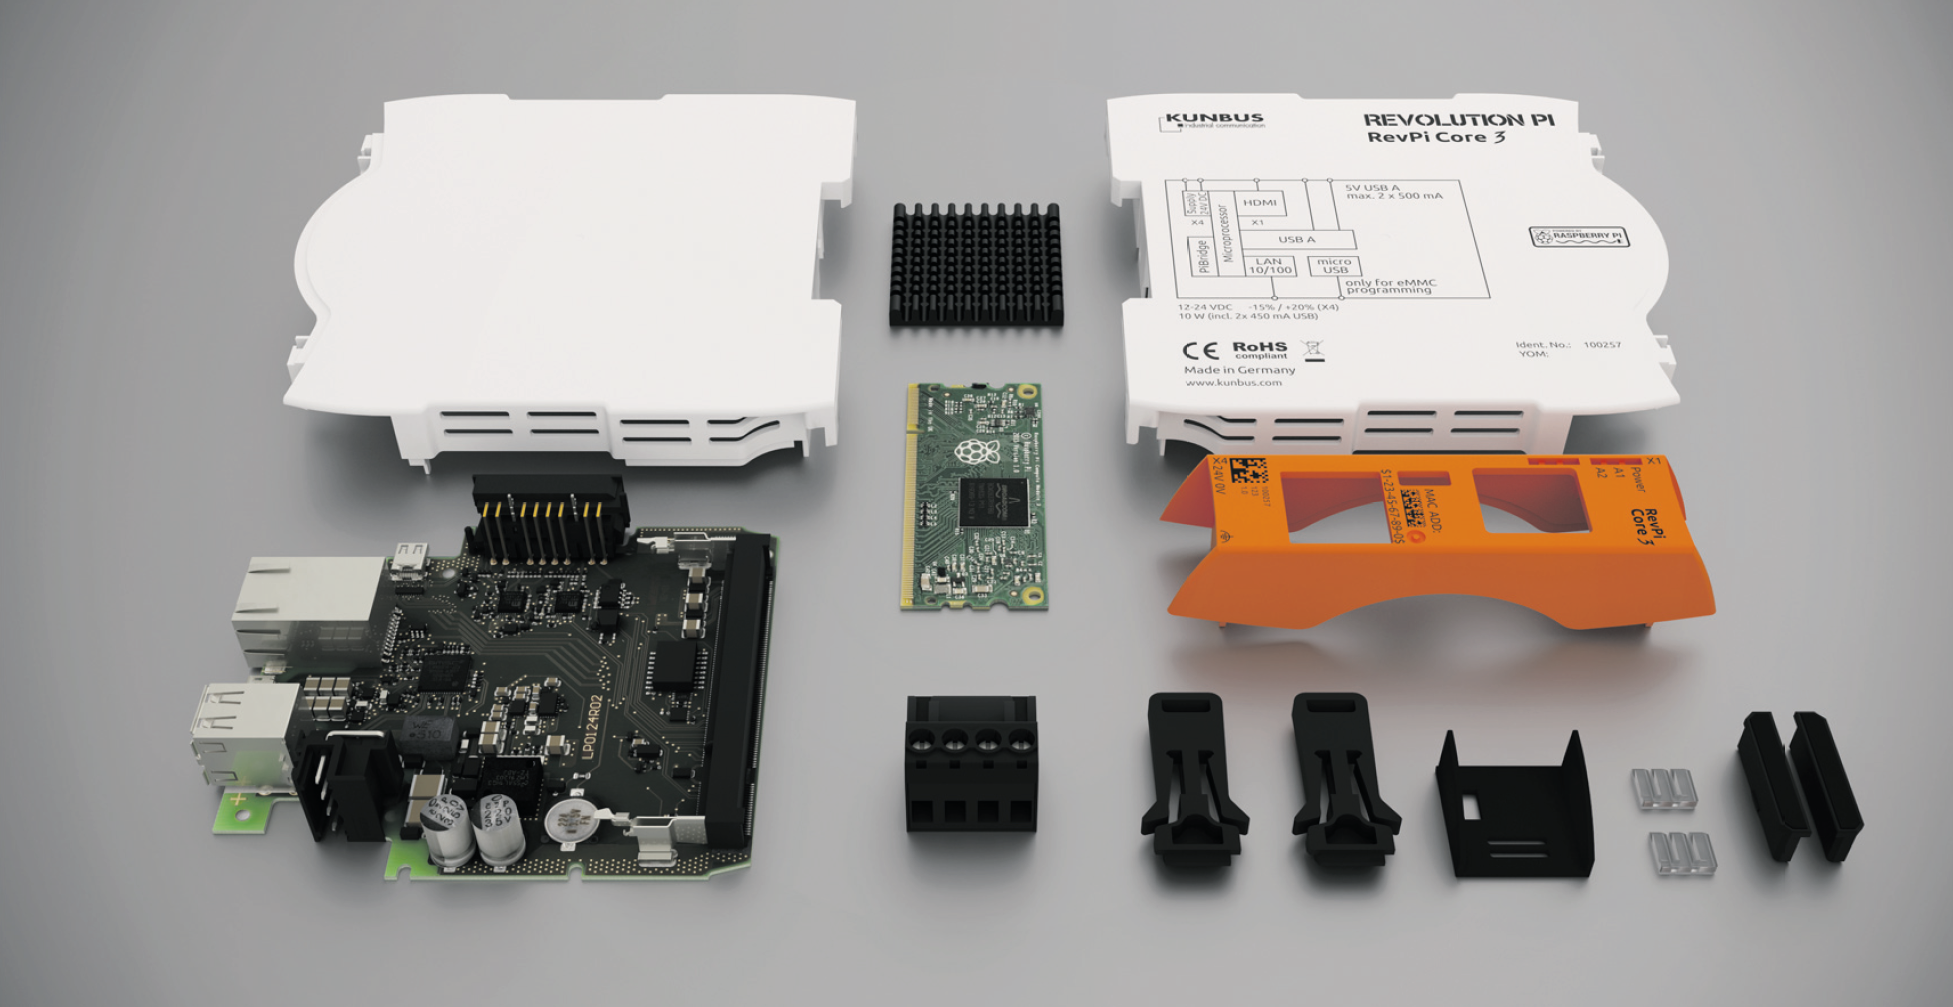
\includegraphics[width=0.85\textwidth]{doc/tex/images/revpi_teardown.png}
    \caption{Der RevPi Core 3 und seine Einzelkomponenten (Quelle: Kunbus)
      \label{fig:revpi-expl}}
\end{figure}

Spezifikationen des RevPi Core 3 \citep[Auswahl, vgl.][S. 1]{datasheet-revpi}:
\begin{itemize}
  \item{Prozessor: BCM2837}
  \item{Taktfrequenz 1,2 GHz}
  \item{Anzahl Prozessorkerne: 4}
  \item{Arbeitsspeicher: 1 GByte}
  \item{eMMC Flash Speicher: 4 GByte}
  \item{Betriebssystem: Angepasstes Raspbian mit RT-Patch}
  \item{RTC mit 24h Pufferung über wartungsfreien Kondensator}
  \item{Treiber / API: Kernel-Treiber schreibt zyklisch Prozessdaten in ein Prozessabbild, Zugriff auf Prozessabbild mittels ioctl-Anfragen oder über Linux-Dateisystem als API zu Fremdsoftware}
  \item{Kommunikationsanschlüsse: 2 x USB 2.0 A, 1 x Micro-USB, HDMI, Ethernet 10/100 Mbit/s}
  \item{Stromversorgung: min. 10,7 V, max. 28,8 V, maximal 10 Watt}
\end{itemize}

Kunbus stellt für den Revolution Pi ein auf Raspbian\footnote{Raspbian ist eine speziell 
für den Raspberry Pi angepasste Variante von Debian.} Stretch basierendes Betriebssystem bereit.
Verwendet wird der Kernel 4.9.76-rt60-v7+ in Verbindung mit dem SMP PREEMPT RT Patch.

\begin{figure}
    \centering
    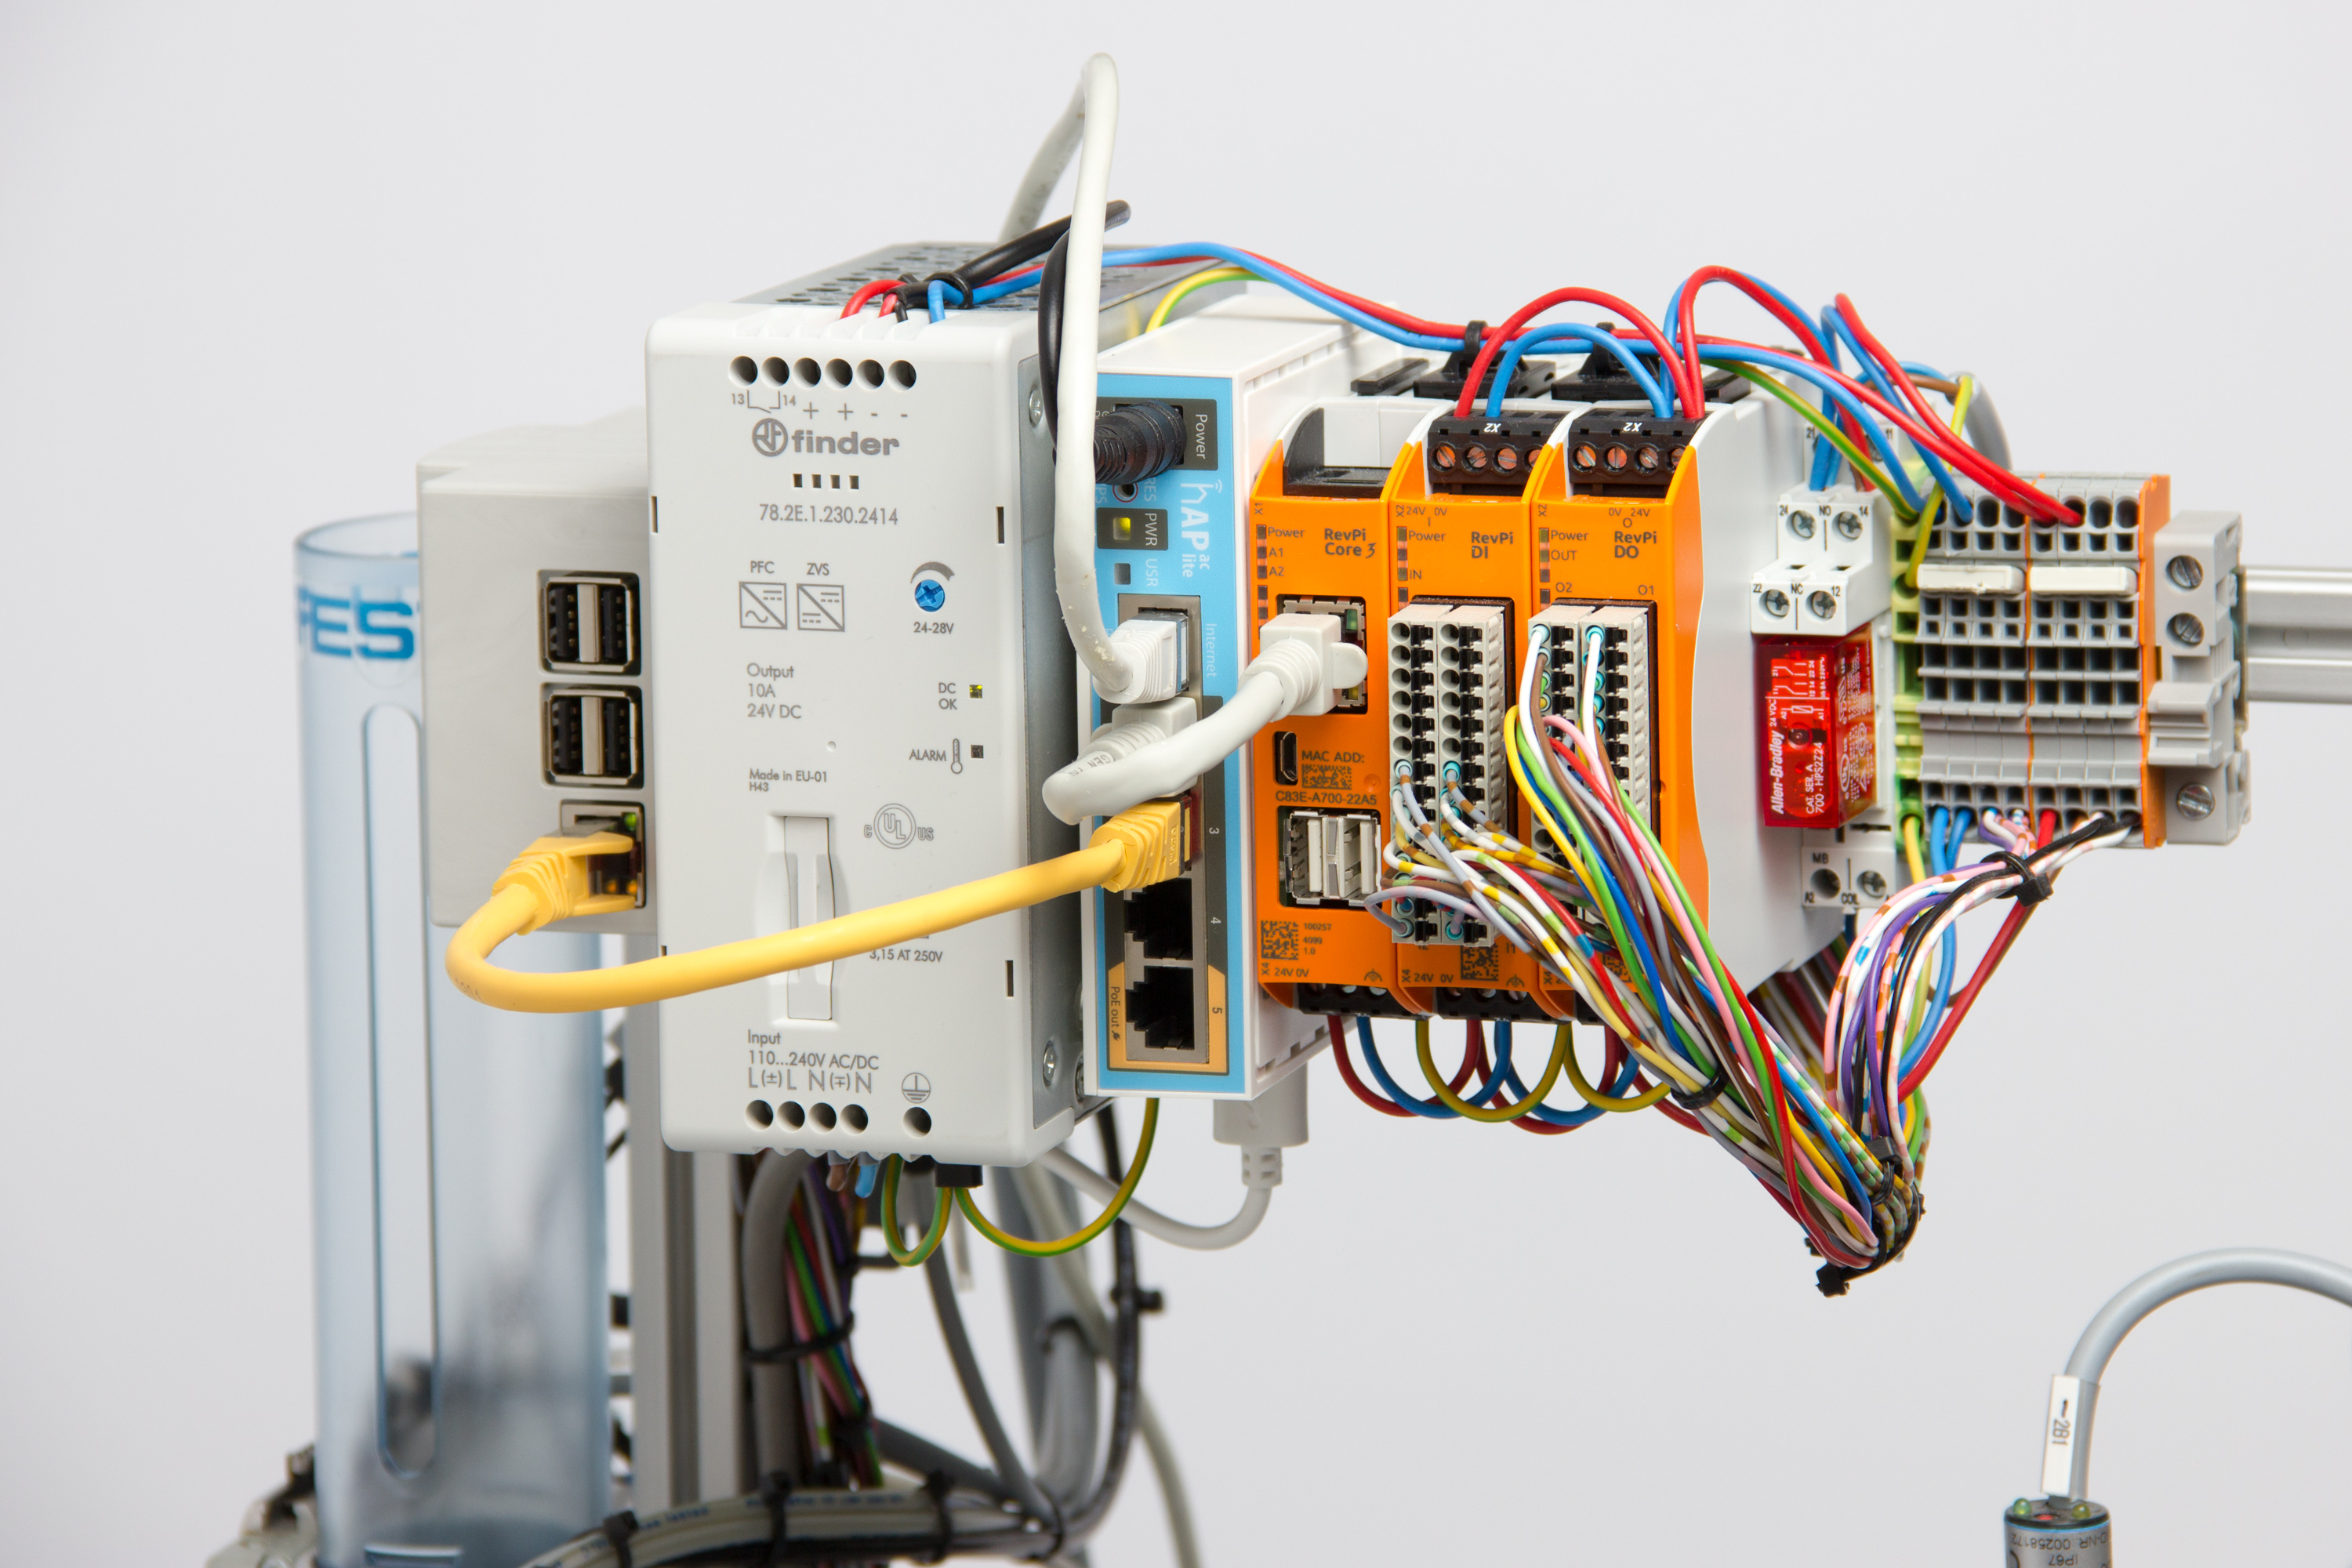
\includegraphics[trim={13cm 5cm 1cm 3cm}, clip, width=0.85\textwidth]{../photos/serverless_plc_img_8}
    \caption{Der Revolution Pi 3 mit digitalen IO-Modulen}
    \label{fig:rev-pi-io}
\end{figure}

Kunbus bietet neben dem sog. Core auch IO- und Gateway-Modulen zur Erweiterung der SPS an, siehe Bild~\ref{fig:rev-pi-io}.
Gateways dienen der Kommunikation mit externen Systemen oder Komponenten
über in der Automatisierungstechnik gängige Protokolle wie PROFIBUS oder EtherCAT. 
IO-Module erlauben die Überwachung und Steuerung von digitalen oder analogen Ein- und Ausgängen (IOs).

Kunbus deklariert die Hardware des Revolution Pi als Open-Source \citep[vgl.][S. 4]{flyer-revpi}. 
Die Schaltpläne des Revolution Pi, genauer die des RevPi Core 3 und der IO-Module, stehen auf der
Website\footnote{\label{downloads}\url{https://revolution.kunbus.com/tutorials/downloads/}} des Herstellers zum 
Download bereit. Eine Lizenz wird nicht angegeben.
Die Raspberry Pi Foundation stellt die Schaltpläne des Compute Modules des weiteren in ihrem Gitub-Repository 
zum Download bereit.

Sowohl die Raspberry Pi Foundation als auch die Kunbus GmbH pflegen aktiv ihre öffentlichen Repositories\footnote{\url{https://github.com/raspberrypi/} resp.~\url{https://github.com/RevolutionPi/}}
auf Github. 

% Kunbus konnte so einige Verbesserungen zum Linux Kernel 4.15 beitragen
% \footnote{siehe \url{https://revolution.kunbus.com/our-contribution-to-linux-4-15/}}.
% \todo{letzten Absatz evtl. weglassen? an sich nicht schlecht, passt aber irgendwie 
% nicht richtig zum Rest und stört den Lesefluss}

\subsubsection{Zugriff auf IO-Module%
        \label{sec:2-io}}
Der Zugriff auf die Ein- und Ausgänge der IO-Module erfolgt über einen RS485-Bus und einen in Form eines Kernel-Moduls bereitgestellten Treiber, genannt piControl. Der RS485-Bus ist über die serielle Schnittstelle des Compute Modules angebunden. 
piControl stellt ein Prozessabbild bereit, welches den physikalischen Zustand der Ein- und Ausgänge der IO-Module repräsentiert.
Das Prozessabbild wird, wie in der Automatisierungstechnik üblich, zyklisch aktualisiert. 
Die angestrebte Zykluszeit beträgt 5ms, kann jedoch je nach Anzahl der angeschlossenen Module auch größer sein. 
Kunbus garantiert bei drei IO-Modulen und zwei Gateway-Modulen eine Zykluszeit von 10 ms \citep[vgl.][]{web-revpi-dio}.
Die garantierte Zykluszeit ermöglicht die Umsetzung von Anwendungen mit harten Echtzeit-Anforderungen.

Fremdanwendungen können über eine Applikationsschnittstelle (API) auf das Prozessabbild zugreifen. 
Hierzu stellt das Kernel-Modul piControl sowohl \lstinline{seek}, \lstinline{read} und \lstinline{write} Methoden zur verfügung, wie auch die Möglichkeit mittels \lstinline{ioctl}-Anfragen gezielt auf einzelne Variablen des Prozessabbildes zuzugreifen.
In der englischsprachigen Wikipedia werden ioctl-Aufrufe wie folgt beschrieben:

\glqq{}The kernel is designed to be extensible, and may accept an extra module called a device driver which runs in kernel space and can directly address the device. An ioctl interface is a single system call by which userspace may communicate with device drivers. [...] The basic kernel can thus allow the userspace to access a device driver without knowing anything about the facilities supported by the device, and without needing an unmanageably large collection of system calls.

[...] ioctl calls provide a convenient way to bridge userspace code to kernel extensions. Kernel extensions can provide a location in the filesystem that can be opened by name, through which an arbitrary number of ioctl calls can be dispatched, allowing the extension to be programmed without adding system calls to the operating system.\grqq{}\citep[vgl.][]{web-wiki-ioctl}

Der Quellcode von piControl steht unter der GNU General Public License Version 2 (GNU GPLv2) und ist 
auf Github verfügbar\footnote{\url{https://github.com/RevolutionPi/piControl}}. Als Einstieg in die 
Entwicklung eigener Steuerungsprogramme liefert Kunbus das C-Programm piTest mit. Dieses verwendet 
piControl und erlaubt dem Nutzer über Kommandozeilen-Parameter die angeschlossenen IO-Module zu steuern.

\begin{figure}[h]
    \centering
    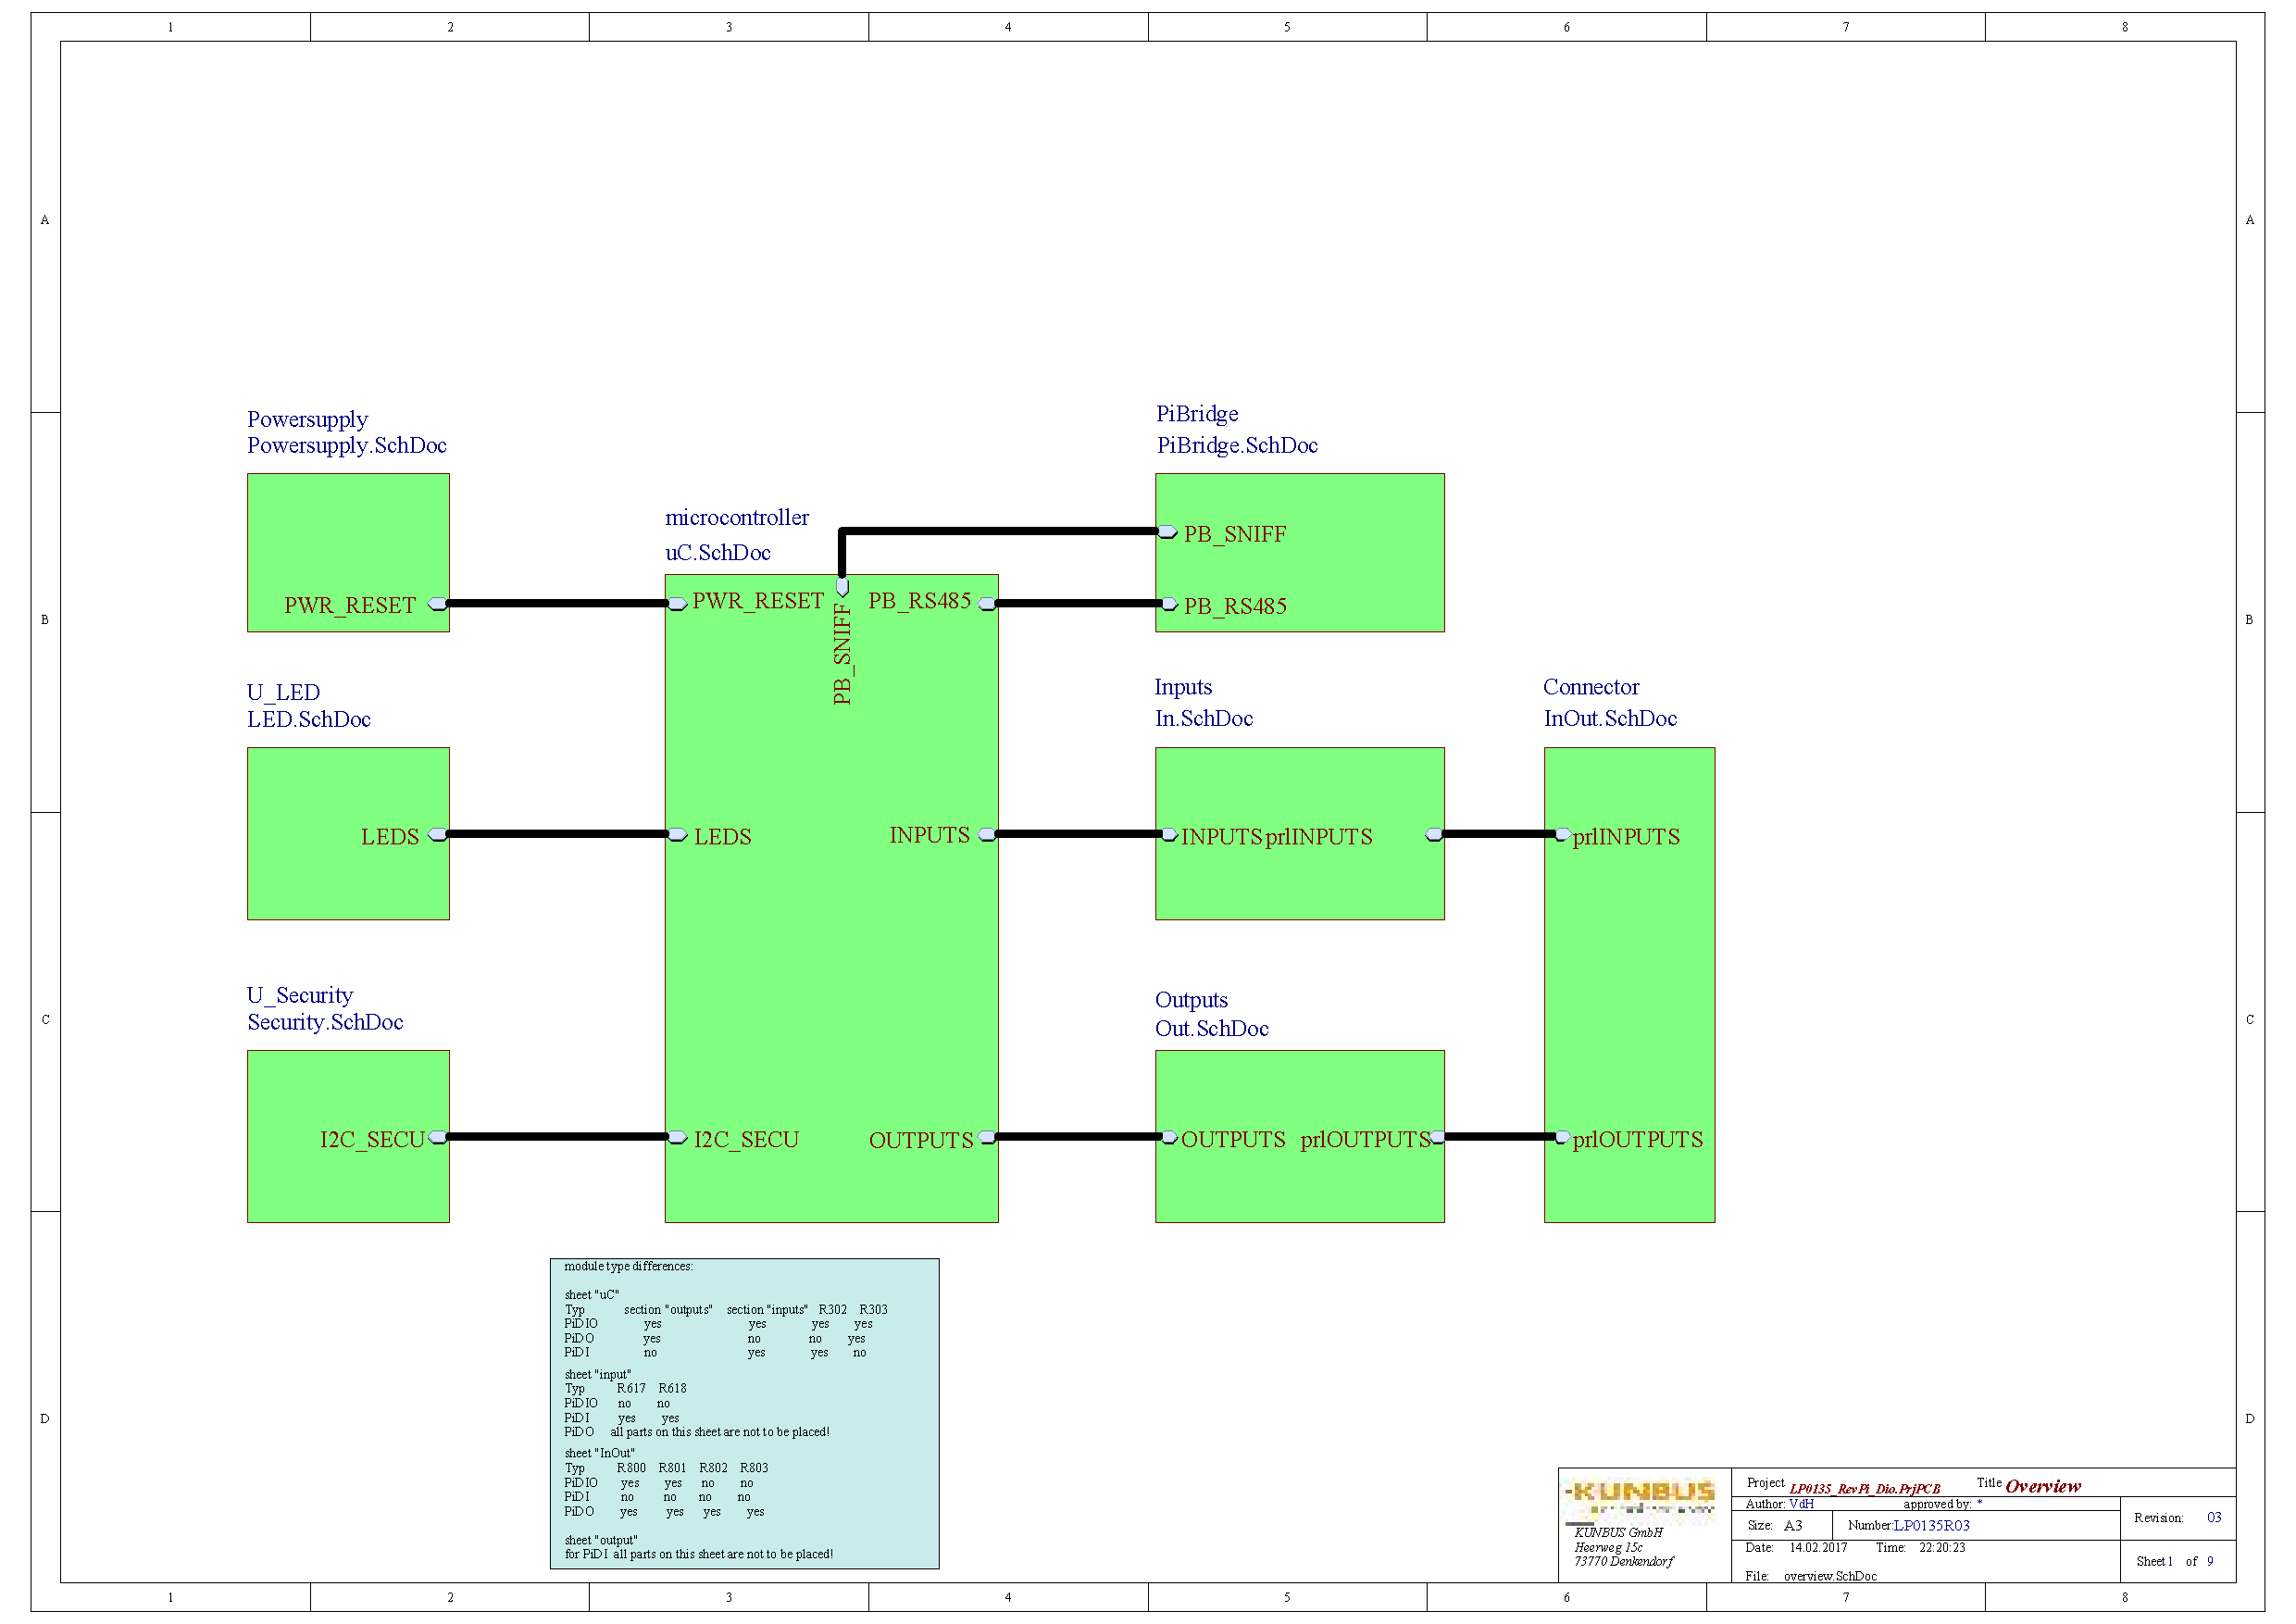
\includegraphics[trim={4cm 7cm 10.5cm 7.3cm}, clip, width=\textwidth]{literature/SchematicPrintsRevPi-DIO}
    \caption{Schematische Darstellung eines DIO-Moduls (Quelle: Kunbus\textsuperscript{\ref{downloads}})
      \label{fig:dio}}
\end{figure}

Jedes der IO-Module stellt ein eigenständiges eingebettetes System dar. Es verfügt
über einen Microcontroller, welcher die IOs bereitstellt und über einen RS485-Bus
mit dem Revolution Pi kommuniziert (siehe Bild~\ref{fig:dio}). 
Kunbus stellt exemplarisch den Quellcode eines DIO-Moduls unter der MIT Lizenz zur
Verfügung\footnote{\url{https://github.com/RevolutionPi/IODeviceExample}}. 


\subsection{Echtzeit und Multitasking unter Linux -- preemptRT und posix%
     \label{sec:2-echtzeit}}
     
Moderne Betriebssysteme realisieren Multitasking i.d.R.\,in Form des präemptiven Multitasking. 
Der Kernel verfügt über einen sog. Scheduler. Dieser priorisiert alle Prozesse und weist ihnen 
Rechenzeit in sog. Time Slots zu. Die Größe der Zeitfenster sowie die Ausführungsreihenfolge 
ist von der Priorität eines Prozesses abhängig. Besonders an einem präemptiven im Gegensatz zu einem kooperativen Scheduler ist dessen Fähigkeit, Tasks während ihrer Ausführung zu unterbrechen bzw. zu pausieren, wenn diese eine bestimmte Dauer überschreiten oder ein höher priorisierter Prozess (bspw. ausgelöst durch einen Interrupt oder durch eine inhärente Periodizität) Rechenleistung benötigt.

Eine Sonderform des präemptiven Multitasking ist das präemptible Multitasking. Hierbei werden auch Teile 
des Kernels als Threads durch den Scheduler ausgeführt. Dieser ist somit in der Lage, auch Prozesse des Kernels
zu unterbrechen, wenn andere Anwendungen Prozessorzeit oder Zugriff auf andere Systemressourcen benötigen
\citep[vgl.][]{web-wiki-praempt}.
     
Der Linux-Kernel implementiert unterschiedliche Präemptions-Modelle \citep[vgl.][/preemption\_models]{web-linuxwiki-basics}:

\begin{itemize}
  \item No Forced Preemption (server):
  Ausgelegt auf maximal möglichen Durchsatz, lediglich Interrupts und
  System-Call-Returns bewirken Präemption.

  \item Voluntary Kernel Preemption (Desktop):
  Neben den implizit bevorrechtigten Interrupts und System-Call-Returns gibt es
  in diesem Modell weitere Abschnitte des Kernels in welchen Preämption explizit
  gestattet ist.

  \item Preemptible Kernel (Low-Latency Desktop):
  In diesem Modell ist der gesamte Kernel, mit Ausnahme sog.~kritischer Abschnitte
  präemptible. Nach jedem kritischen Abschnitt gibt es einen impliziten Präemptions-Punkt.

  \item Preemptible Kernel (Basic RT):
  Dieses Modell ist dem zuvor genannten sehr ähnlich, hier sind jedoch alle Interrupt-Handler
  als eigenständige Threads ausgeführt.

  \item Fully Preemptible Kernel (RT):
  Wie auch bei den beiden zuvor genannten Modellen ist hier der gesamte Kernel
  präemtible. Die Anzahl und Dauer der nicht-präemtiblen kritischen Abschnitte
  ist auf ein notwendiges Minimum beschränkt. Alle Interrupt-Handler sind als
  eigenständige Threads ausgeführt, Spinlocks durch Sleeping-Spinlocks und Mutexe
  durch sog.~RT-Mutexe ersetzt.

\end{itemize}

Lediglich ein präemtibler Kernel kann hartes Echtzeit-Verhalten realisieren, 
da nur hier eine maximale Antwortzeit garantiert werden kann.
Viele Prozesse in der Automatisierungstechnik erfordern harte Echtzeit. 
Eine verspätete Antwort auf eine Anfrage, 
wie etwa das Signal eines Lagenendschalters oder eines Notausschalters kann hier nicht nur über
den Erfolg eines Prozesses, sondern auch über das Leben der daran beteiligten Mitarbeiter entscheiden.
Für weiterführende Erklärungen bzgl.\,Echtzeit, Mutexen und 
Spinlocks sei an dieser Stelle auf die Vorlesung verwiesen~\citep{script-peter}.


\subsubsection{preemptRT%
        \label{sec:2-preemptRT}}

Der Kernel des auf dem Revolution Pi installierten Raspbian mit PREEMP\_RT Patch fällt 
in die Kategorie des \glqq{}Fully Preemptible Kernels\grqq{} (siehe Abschnitt \ref{sec:2-echtzeit}).
Das zugrunde liegende Prinzip lässt sich wie folgt formulieren: Nur Code, welcher absolut nicht-präemtible sein darf, ist es
gestattet nicht-präemtible zu sein. Ziel ist folglich, die Menge des nicht-präemtiblen 
Codes im Linux-Kernel auf das absolut notwendige Minimum zu reduzieren.

Dies wird durch Verwendung folgender Mechanismen erreicht~\citep[vgl.][]{web-linuxwiki-details}:

\begin{itemize}
  \item Hochauflösende Timer
  \item Sleeping Spinlocks
  \item Threaded Interrupt Handlers
  \item rt\_mutex
  \item RCU
\end{itemize}

Diese Mechanismen sind bspw. im Linux-Wiki\footnote{siehe \url{https://wiki.linuxfoundation.org/realtime/documentation/technical_details}} ausführlich beschrieben.

\subsubsection{POSIX%
        \label{sec:2-posix}}
Das Portable Operating System Interface (POSIX) bezeichnet eine Sammlung von Standards, 
welche auf dem Unix-System basieren, jedoch nicht auf dieses beschränkt sind.

Der Wechsel zwischen verschiedenen Unix-Distributionen brachte oft Kompatibilitätsprobleme mit sich. 
Dieser Mangel an Portabilität erschwerte Benutzern und Entwicklern die Verwendung bzw. Bereitstellung 
von Software auf unterschiedlichen Systemen. 
Das Institut für Elektrotechnik und Elektronik (IEEE) begann 1984 mit der Entwicklung des Unix-Standards.
Sie entwickelten das, was heute als Single UNIX Specification bekannt ist und allgemein als POSIX bezeichnet wird~\citep[vgl.][]{web-debianwiki-posix}.
Das Konsortium \glqq{}The Open Group\grqq{} überwacht die weitere Entwicklung dieses Standards.
Ferner stellt es einen Teil der POSIX-Spezifikation frei zur Verfügung~\citep[vgl.][]{web-opengroup-posix}.

Die aktuelle Version POSIX.1-2017 ist verfügbar als IEEE Standard 1003.1-2017 sowie in Form der \glqq{}The Open Group Technical Standard Base Specifications\grqq{}, Ausgabe 7. POSIX.1-2017 definiert eine Standard-Betriebssystemschnittstelle und -umgebung, einschließlich eines Befehlsinterpreters (auch Shell genannt) und gängiger Dienstprogramme zur Unterstützung der Portabilität von Anwendungen auf Quellcode-Ebene. POSIX.1-2017 ist sowohl für Anwendungsentwickler als auch für Systemimplementierer gedacht und umfasst vier Hauptkomponenten \citep[vgl.][]{web-opengroup-overview}:
\begin{itemize}
    \item Basisdefinitionen:\\
          Allgemeine Begriffe, Konzepte und Schnittstellen einschließlich Hilfskonventionen und C-Headern
          
    \item Systemschnittstellen:\\
          Definitionen für Systemdienstfunktionen und Unterprogramme, C-spezifische Systemdienste, Portabilität
        
    \item Shell und Dienstprogramme:\\
          Definitionen für eine Schnittstelle zur Befehlsinterpretation von Diensten und gängige Hilfsprogramme
    
    \item Begründungen und Historie
\end{itemize}

Debian basiert auf Linux und verwendet den Linux-Kernel. Linux ist zu großen Teilen POSIX-kompatibel. Debian ist jedoch nicht POSIX-zertifiziert, da diese Zertifizierung mit hohen Kosten verbunden ist\citep[vgl.][Kapitel 4.4.]{web-debian-faq}.

Beide Kernkomponenten des in dieser Arbeit vorgestellten Projektes nutzen Komponenten von Linux, 
welche an den POSIX-Standard angelehnt sind: open62541 verwendet u.a.\,POSIX-Threads und
Mutexe~\citep[vgl.][pthread.h]{web-opengroup-pthread}, piControl nutzt POSIX-Semaphoren
\citep[vgl.][semaphore.h]{web-opengroup-semaphore}. 


\subsection{OPC-UA und open62541%
     \label{sec:2-opc}}
In diesem Abschnitt sollen Möglichkeiten des Datenaustausch zwischen Komponenten der
Automatisierungstechnik vorgestellt werden. OPC-UA stellt einen offenen, IP-basierten Kommunikationsstandard
für Sensoren und Steuerungen dar. open62541 ist eine freie Client- sowie Server-Implementierung dieses
Standards, geschrieben in C.


\subsubsection{OPC UA%
        \label{sec:2-opcua}}

Open Platform Communications (OPC) ist eine Familie von Standards zur herstellerunabhängigen
Kommunikation von Maschinen (M2M) in der Automatisierungstechnik. Die sog. OPC Task Force, zu deren
Mitgliedern verschiedene etablierte Firmen der Automatisierungsindustrie gehören, veröffentlichte
die OPC Specification Version 1.0 im August 1996.
Motiviert ist dieser offene Standard durch die Erkenntniss, dass die Anpassung der
zahlreichen Herstellerstandards an individuelle Infrastrukturen und Anlagen einen
großen Mehraufwand verursachen.
Die Wikipedia beschreibt das Anwendungsgebiet für OPC wie folgt \citep[vgl.][]{web-wiki-opc}:

\glqq{}OPC wird dort eingesetzt, wo Sensoren, Regler und Steuerungen verschiedener Hersteller
ein gemeinsames Netzwerk bilden. Ohne OPC benötigten zwei Geräte zum Datenaustausch
genaue Kenntnis über die Kommunikationsmöglichkeiten des Gegenübers. Erweiterungen
und Austausch gestalten sich entsprechend schwierig. Mit OPC genügt es, für jedes
Gerät genau einmal einen OPC-konformen Treiber zu schreiben. Idealerweise wird
dieser bereits vom Hersteller zur Verfügung gestellt. Ein OPC-Treiber lässt sich
ohne großen Anpassungsaufwand in beliebig große Steuer- und Überwachungssysteme
integrieren.

OPC unterteilt sich in verschiedene Unterstandards, die für den jeweiligen Anwendungsfall
unabhängig voneinander implementiert werden können. OPC lässt sich damit verwenden
für Echtzeitdaten (Überwachung), Datenarchivierung, Alarm-Meldungen und neuerdings
auch direkt zur Steuerung (Befehlsübermittlung).\grqq{}

OPC basiert in der ursprünglichen Spezifikation (auch als OPC DA bezeichnet) auf Microsofts DCOM-Spezifikation.
DCOM macht Funktionen und Objekte einer Anwendung anderen Anwendungen im Netzwerk
zugänglich. Der OPC-Standard definiert entsprechende DCOM-Objekte um mit anderen
OPC-Anwendungen Daten austauschen zu können. Die Verwendung von DCOM bindet Anwender
jedoch an Betriebssysteme von Microsoft. 

\begin{figure}
    \centering
    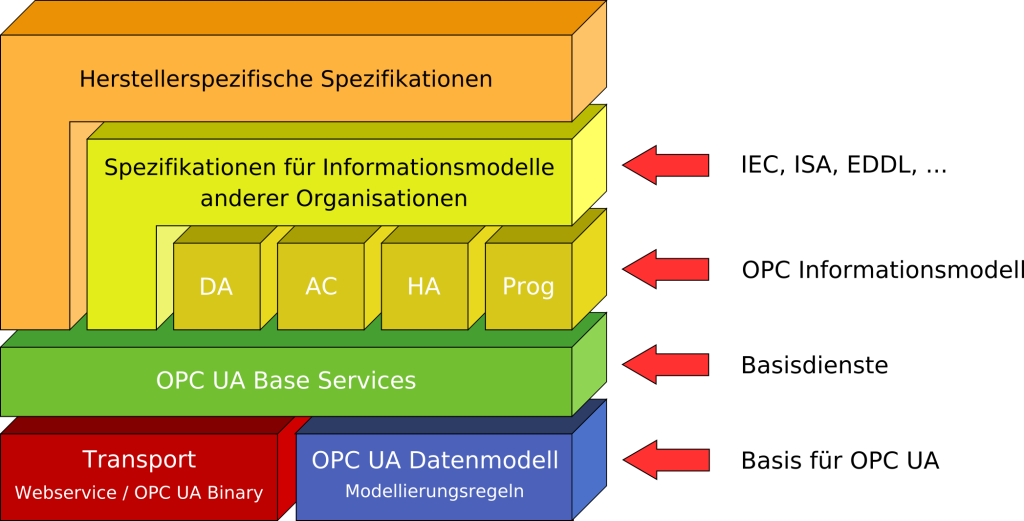
\includegraphics[width=0.85\textwidth]{images/UA_Architecture_1024.png}
    \caption{Die OPC Unified Architecture. Grafik von Gerhard Gappmeier - ascolab GmbH, CC BY-SA 3.0}
    \label{fig:opc-unified-architecture}
\end{figure}
% Evtl Grafik: Von Gerhard Gappmeier - ascolab GmbH, CC BY-SA 3.0, https://de.wikipedia.org/w/index.php?curid=1892069

Die ursprüngliche OPC Spezifikation wurde 2006 durch die Entwicklung der 
OPC Unified Architecture (OPC UA) überholt. 
Diese zeichnet sich durch eine Service-orientierte Architektur (SOA) aus, deren Struktur
aus mehreren Schichten besteht, siehe Abbilung~\ref{fig:opc-unified-architecture}. 
Über der untersten Schicht, dem Betriebssystem des Servers, verbindet eine Portabilitäts-Schicht 
den sog.\, UA ANSI C Stack mit einer API. Diese API kann bspw.\,in C++ geschrieben sein, 
und erlaubt die Anbindung der obersten Schicht, der Anwendungsschicht~\citep[vgl.][]{web-spec-opc}.
OPC UA setzt auf einem eigenen Kommunikationsstack auf; die Verwendung von DCOM
und damit die Bindung an Microsoft wurden aufgelöst.

Neben Architektur und Kommunikationsschnittstellen wird in der OPC Spezifikation auch ein 
Informationsmodell definiert. Die deutschsprachige Wikipedia beschreibt dieses wie folgt: 

\glqq{}Das OPC[-UA]-Informationsmodell ist nicht mehr nur eine Hierarchie aus Ordnern, Items
und Properties. Es ist ein sogenanntes Full-Mesh-Network aus Nodes, mit dem neben
den Nutzdaten eines Nodes auch Meta- und Diagnoseinformationen repräsentiert werden. [...]
Ein Node ähnelt einem Objekt aus der objektorientierten Programmierung. Ein Node
kann Attribute besitzen, die gelesen werden können. Es ist möglich Methoden zu definieren und aufzurufen. [...]
Weiterhin werden Events unterstützt, die versendet werden können
(AE (Alarms \& Events), DA DataChange), um bestimmte Informationen zwischen Geräten
auszutauschen. Ein Event besitzt unter anderem einen Empfangszeitpunkt, eine Nachricht
und einen Schweregrad. Die o.\,g. Nodes werden sowohl für die Nutzdaten als auch
alle anderen Arten von Metadaten verwendet. Der damit modellierte OPC-Adressraum
beinhaltet nun auch ein Typmodell, mit dem sämtliche Datentypen spezifiziert werden.\grqq{}


\subsubsection{open62541%
        \label{sec:2-open62541}}
open62541 ist eine offene und freie Implementierung von OPC UA. 
Die in C geschriebene Bibliothek stellt eine beständig zunehmende Anzahl der im OPC UA Standard definierten
Funktionen bereit. Sie kann sowohl zur Erstellung von OPC-Servern als auch von -Clients
genutzt werden. Ergänzend zu der unter der Mozilla Public License v2.0 lizensierten
Bibliothek stellt das open62541 Projekt auch Beispielprogramme unter einer CC0 Lizenz
zur Verfügung.
Zu den Unterstützern des Projektes zählen u.a.\, die RWTH Aachen, das Frauenhofer IOSB sowie die TU Dresden.

Die Bibliothek eignet sich auch für die Entwicklung auf eingebetteten Systemen und
Microcontrollern. Die Größe einer Server-Binary kann weniger als 100kB betragen.

Folgende Auswahl an Eigenschaften und Funktionen zeichnet die in dieser Arbeit verwendete
Version 0.3 von open62541 aus:
\begin{itemize}
  \item Kommunikationionsstack
  \begin{itemize}
      \item OPC UA Binär-Protokoll (HTTP oder SOAP werden gegenwärtig nicht unterstützt)
      \item Austauschbare Netzwerk-Schicht, welche die Verwendung eigener Netzwerk-APIs
      erlaubt.
      \item Verschlüsselte Kommunikationion
      \item Asynchrone Dienst-Anfragen im Client
  \end{itemize}
  \item Informationsmodell
  \begin{itemize}
    \item Unterstützung aller OPC UA Node-Typen, inkl.~Methoden
    \item Hinzufügen und Entfernen von Nodes und Referenzen zur Laufzeit.
    \item Vererbung und Instanziierung von Objekt- und Variablentypen
    \item Zugriffskontrolle auch für einzelne Nodes
  \end{itemize}
  \item Subscriptions
  \begin{itemize}
    \item Erlaubt die Überwachung (subscriptions / monitoreditems)
    \item Sehr geringer Ressourcenbedarf pro überwachtem Wert
  \end{itemize}
  \item Code-Generierung auf XML-Basis
  \begin{itemize}
    \item Erlaubt die Erstellung von Datentypen
    \item Erlaubt die Generierung des serverseitigen Informationsmodells
  \end{itemize}
\end{itemize}

Weiterführende Informationen und Code-Beispiele bietet die ausführliche Dokumentation des Projektes~\citep[siehe]{web-open62541} sowie der kommentierte Quelltext.

%% % Imports nur für Referenzenauflösung während des Schreibens! Vorm Kompilieren auskommentieren!
% \bibliography{0_hauptdatei}
% % Mit \section{...} eröffnen wir einen neuen Abschnitt.
% Der Befehl setzt nicht nur den Text in einer größeren,
% fetten Schrift, sondern sorgt außerdem dafür, daß er im
% Inhaltsverzeichnis erscheint.
%
% Mit \label{...} erzeugen wir einen Bezeichner, mit dessen Hilfe
% wir später auf die Nummer des Abschnitts verweisen können (nämlich
% mit~\ref{...}).
%
% Das Kommentarzeichen hinter „Übersicht“ dient dazu, ein
% Leerzeichen zwischen „Übersicht“ und dem \label-Befehl
% zu vermeiden, das andernfalls sichtbar würde – z.B. im
% Inhaltsverzeichnis.
%

% % Imports nur für Referenzenauflösung während des Schreibens! Vorm Kompilieren auskommentieren!
% \bibliography{0_hauptdatei}
% \input{1_einleitung}
%\input{2_grundlagen}
%\input{3_konzeption}
%\input{4_implementierung}
%\input{5_tests}
%\input{6_zusammenfassung}
% % Ende Imports

\section{Einleitung und Motivation%
  \label{sec:1-einleitung}}
Ziel dieses Projektes ist die Integration eines OPC-Servers mit einer auf Linux
basierenden speicherprogrammierbaren Steuerung (SPS). Angeschlossen an diese SPS
ist jeweils ein digitales Ein-/\,bzw.~Ausgabemodul. Die von diesen bereitgestellten
Ein-/\, bzw.~Ausgänge (IO) sollen in der Datenstruktur des OPC-Servers abgebildet
und über diesen für OPC-Clients les-/\,und schreibar sein. Weiterhin sollen einige
Funktionen zur Überwachung und Steuerung der an die SPS angeschlossenen Aktoren
und Sensoren direkt im OPC-Server implementiert werden.
Hiermit stellt dieses Projekt eine der Grundlagen für ein übergeordnetes Projekt,
die cloudbasierte Steuerung eines miniaturisierten Produktions-Systems, dar.

Der hier verwendete OPC-Server ist Teil des sog. open62541 Projekts. Er ist in C
geschrieben und implementiert bereits einen großen Teil der im OPC-UA-Standard
spezifizierten Funktionen.
Als SPS findet ein Revolution Pi 3 der Firma Kunbus Verwendung. Dieser integriert
ein sog. Compute Module der Raspberry Pi Foundation in ein industrietaugliches
Gehäuse und erlaubt die Erweiterung mittels IO- oder Gateway-Modulen. Über diese
erfolgt die Kommunikation mit weiteren Komponenten der Automatisierungstechnik.

Motiviert ist dieses Projekt durch die Beobachtung, dass die Verbreitung offener
Standards sowie freier Software auch in der Automatisierungstechnik zunimmt.
Linux ist ein freies Betriebssystem, OPC-UA ein offen zugänglicher, aktiv gepflegter
und weit verbreiteter Standard. Der Raspberry Pi findet sowohl bei Hobby-Anwendern als
auch in den Bereichen Forschung und Entwicklung sowie bei industriellen Anwendern
Verwendung. Dieses Projekt stellt somit eine für unterschiedliche Anwender interessante
Entwicklung dar.

Im Anschluss an diese einleitende Übersicht im Abschnitt~\ref{sec:1-einleitung} folgt
die Darstellung der wichtigsten Grundlagen in Abschnitt~\ref{sec:2-grundlagen}.
Aufbauend auf diesen Grundlagen folgt die konzeptuelle Ausarbeitung im Abschnitt~\ref{sec:3-konzeption}.
Die Umsetzung wird im Abschnitt~\ref{sec:4-implementierung} erläutert.
Die Leistungsfähigkeit der Implementierung wird in Abschnitt~\ref{sec:5-tests} untersucht.
Eine Zusammenfassung und ein Ausblick schließen die Arbeit in
Abschnitt~\ref{sec:6-fazit} ab. Eventuell noch benötigte Anhänge
finden sich in den Anhängen [...] bis [...].

% % % Imports nur für Referenzenauflösung während des Schreibens! Vorm Kompilieren auskommentieren!
% \bibliography{0_hauptdatei}
% \input{1_einleitung}
% \input{2_grundlagen}
% \input{3_konzeption}
% \input{4_implementierung}
% \input{5_tests}
% \input{6_zusammenfassung}
% % Ende Imports

\section{Grundlagen%
  \label{sec:2-grundlagen}}
Die folgenden Abschnitte bieten einen Überblick über die Verwendung offener Betriebssysteme und
Schnittstellen in der Automatisierungstechnik.
In Abschnitt~\ref{sec:2-sps} wird am Beispiel des Revolution Pi eine modulare Steuerung 
auf Basis von Linux vorgestellt. Ferner werden in Abschnitt~\ref{sec:2-echtzeit} die Themen Echtzeitfähigkeit und Portabilität von Software behandelt.

Eine große Zahl an Systemen in der Automatisierungstechnik ist heutzutage als eine Menge von Subsystemen mit
jeweils eigenem Speicher und Rechenleistung zu betrachten. Die zunehmende Komplexität von Fertigungsabläufen in Verbindung mit einer stetig abnehmenden Losgröße erfordert eine immer umfangreichere Kommunikation zwischen diesen Subsystemen.
Dies gelingt, insbesondere bei Verwendung von Komponenten unterschiedlicher Hersteller, nur mittels offener und flexibler Schnittstellen. OPC-UA stellt eine solche Schnittstelle dar und wird in Abschnitt~\ref{sec:2-opc} vorgestellt.

\subsection{Speicherprogrammierbare Steuerung auf Linux-Basis%
     \label{sec:2-sps}}
In diesem Abschnitt wird mit dem Revolution Pi eine Hard- und Softwarelösung zur Verwendung von Linux als Steuerung in der
Automatisierungstechnik vorgestellt.

\subsubsection{Kunbus Revolution Pi%
        \label{sec:2-revpi}}
Als Revolution Pi (RevPi) vertreibt die Firma Kunbus GmbH eine modulare, speicherprogrammierbare 
Steuerung (SPS). Zentrales Element dieser SPS ist der sog. RevPi Core, hier in der Version 3.
Kernkomponente des RevPi Core 3 ist das von der Raspberry Pi Foundation entwickelte und vertriebene 
Raspberry Pi Compute Module 3 (CM3, siehe Bild~\ref{fig:revpi-expl}. 
Die Architektur des CM3 ist weitgehend identisch zu der des allgemein bekannten Raspberry Pi 3.
Der RevPi Core 3 profitiert daher von dem selben großen Angebot an Software
und Unterstützung wie der Raspberry Pi. Er ergänzt dessen Hardware jedoch um eine 24V
Spannungsversorgung und die Möglichkeit der Erweiterung durch mehrere, zur industriellen 
Verwendung geeignete Ein- und Ausgabemodule (IO-Module. Die Integration dieser Merkmale in ein robustes Gehäuse 
mit Aufnahme für eine DIN-Schiene ermöglicht die Verwendung im industriellen Umfeld.

\begin{figure}[h]
    \centering
    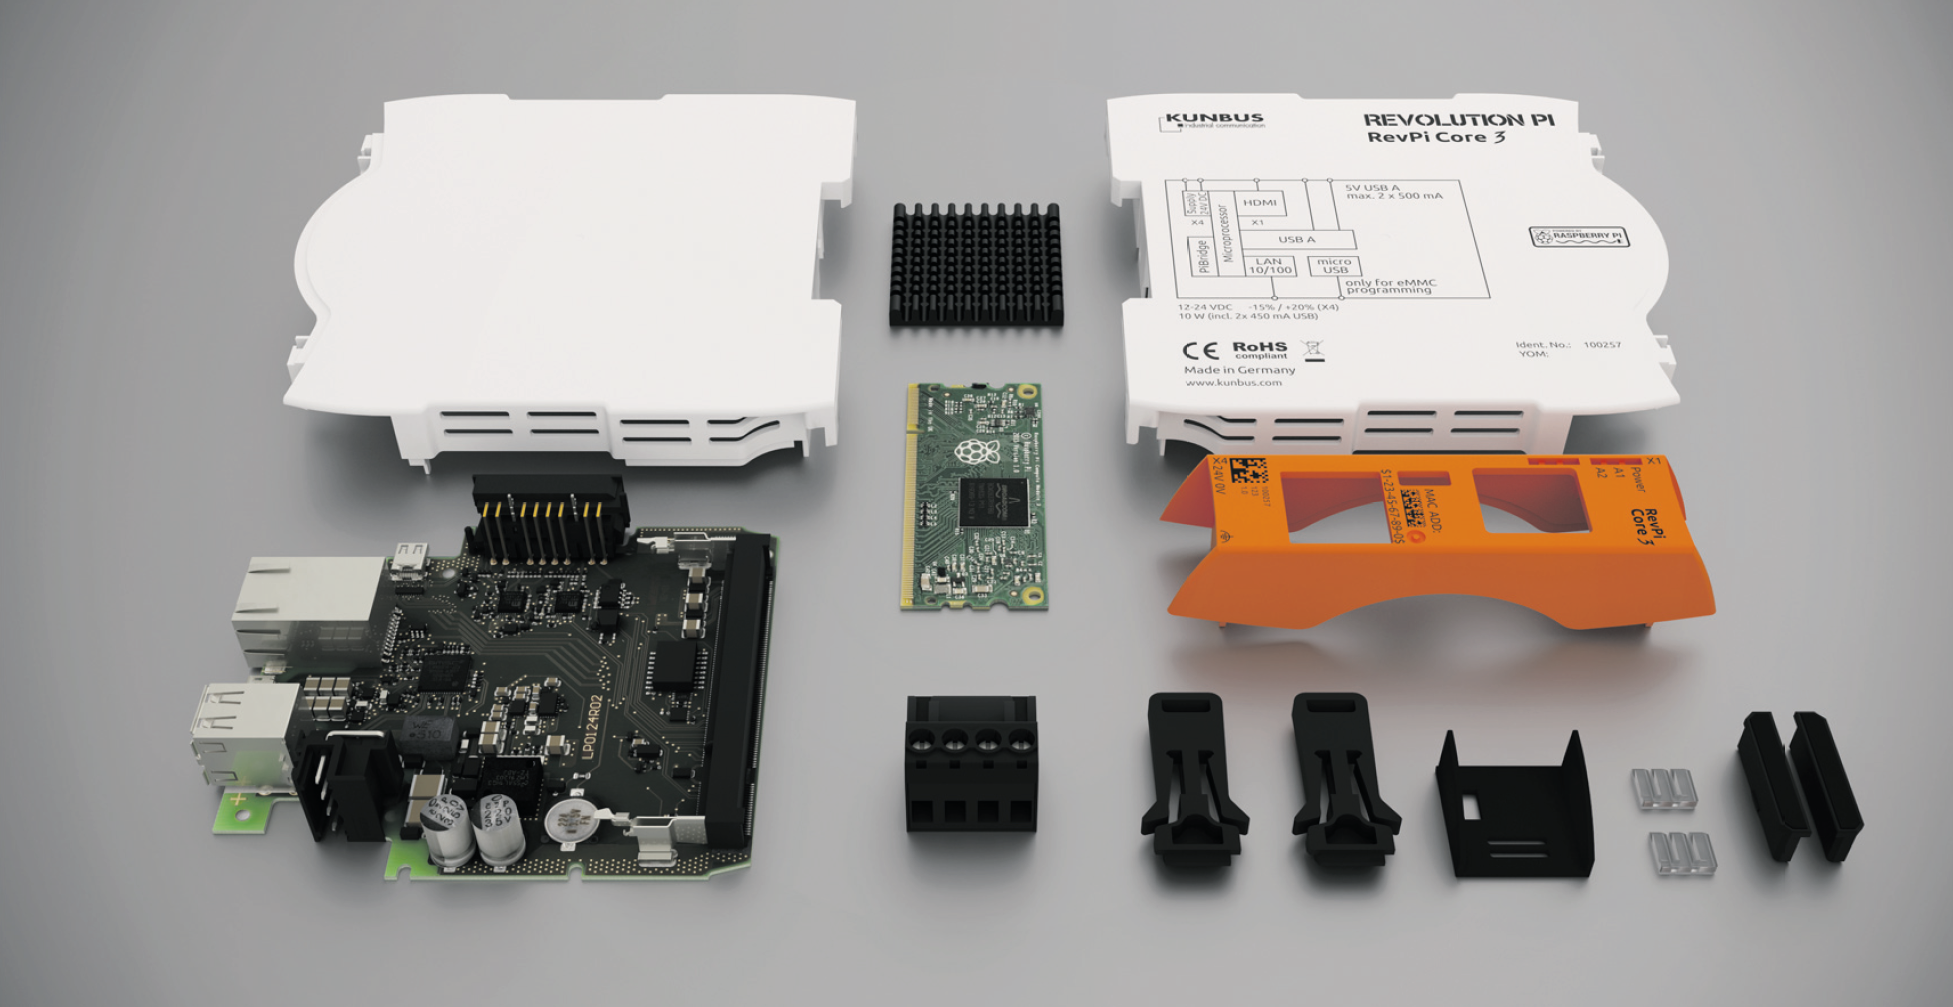
\includegraphics[width=0.85\textwidth]{doc/tex/images/revpi_teardown.png}
    \caption{Der RevPi Core 3 und seine Einzelkomponenten (Quelle: Kunbus)
      \label{fig:revpi-expl}}
\end{figure}

Spezifikationen des RevPi Core 3 \citep[Auswahl, vgl.][S. 1]{datasheet-revpi}:
\begin{itemize}
  \item{Prozessor: BCM2837}
  \item{Taktfrequenz 1,2 GHz}
  \item{Anzahl Prozessorkerne: 4}
  \item{Arbeitsspeicher: 1 GByte}
  \item{eMMC Flash Speicher: 4 GByte}
  \item{Betriebssystem: Angepasstes Raspbian mit RT-Patch}
  \item{RTC mit 24h Pufferung über wartungsfreien Kondensator}
  \item{Treiber / API: Kernel-Treiber schreibt zyklisch Prozessdaten in ein Prozessabbild, Zugriff auf Prozessabbild mittels ioctl-Anfragen oder über Linux-Dateisystem als API zu Fremdsoftware}
  \item{Kommunikationsanschlüsse: 2 x USB 2.0 A, 1 x Micro-USB, HDMI, Ethernet 10/100 Mbit/s}
  \item{Stromversorgung: min. 10,7 V, max. 28,8 V, maximal 10 Watt}
\end{itemize}

Kunbus stellt für den Revolution Pi ein auf Raspbian\footnote{Raspbian ist eine speziell 
für den Raspberry Pi angepasste Variante von Debian.} Stretch basierendes Betriebssystem bereit.
Verwendet wird der Kernel 4.9.76-rt60-v7+ in Verbindung mit dem SMP PREEMPT RT Patch.

\begin{figure}
    \centering
    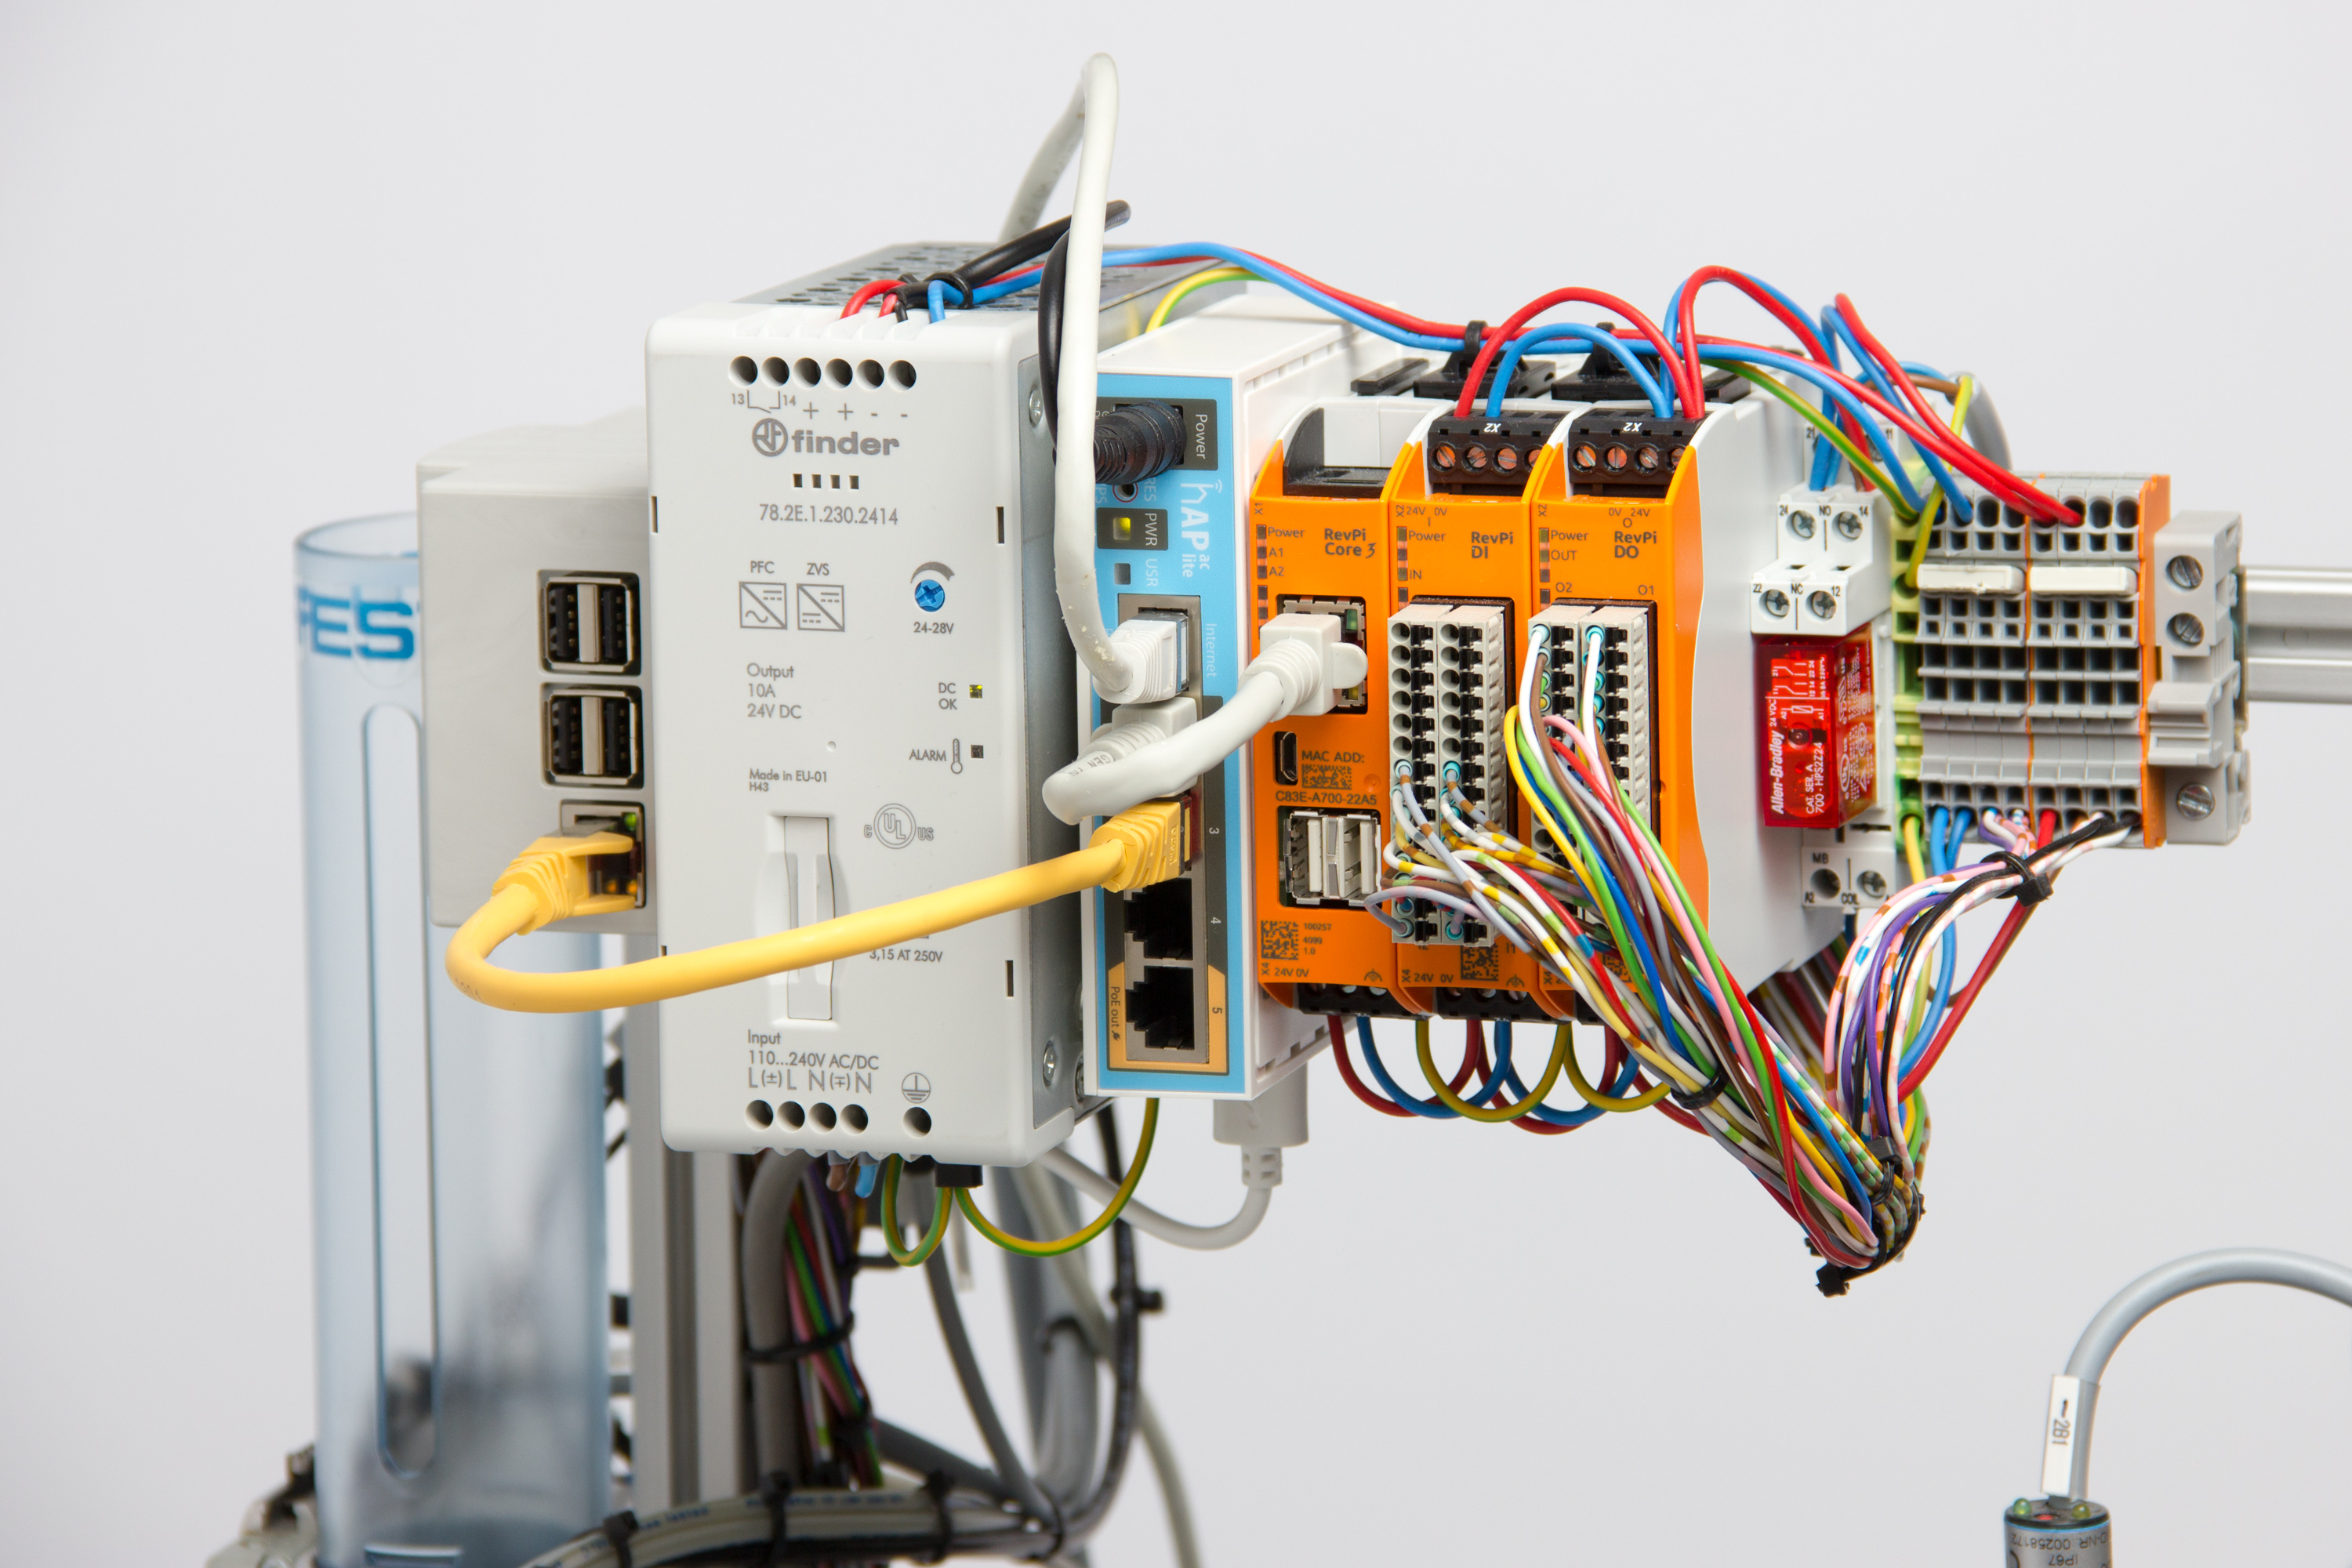
\includegraphics[trim={13cm 5cm 1cm 3cm}, clip, width=0.85\textwidth]{../photos/serverless_plc_img_8}
    \caption{Der Revolution Pi 3 mit digitalen IO-Modulen}
    \label{fig:rev-pi-io}
\end{figure}

Kunbus bietet neben dem sog. Core auch IO- und Gateway-Modulen zur Erweiterung der SPS an, siehe Bild~\ref{fig:rev-pi-io}.
Gateways dienen der Kommunikation mit externen Systemen oder Komponenten
über in der Automatisierungstechnik gängige Protokolle wie PROFIBUS oder EtherCAT. 
IO-Module erlauben die Überwachung und Steuerung von digitalen oder analogen Ein- und Ausgängen (IOs).

Kunbus deklariert die Hardware des Revolution Pi als Open-Source \citep[vgl.][S. 4]{flyer-revpi}. 
Die Schaltpläne des Revolution Pi, genauer die des RevPi Core 3 und der IO-Module, stehen auf der
Website\footnote{\label{downloads}\url{https://revolution.kunbus.com/tutorials/downloads/}} des Herstellers zum 
Download bereit. Eine Lizenz wird nicht angegeben.
Die Raspberry Pi Foundation stellt die Schaltpläne des Compute Modules des weiteren in ihrem Gitub-Repository 
zum Download bereit.

Sowohl die Raspberry Pi Foundation als auch die Kunbus GmbH pflegen aktiv ihre öffentlichen Repositories\footnote{\url{https://github.com/raspberrypi/} resp.~\url{https://github.com/RevolutionPi/}}
auf Github. 

% Kunbus konnte so einige Verbesserungen zum Linux Kernel 4.15 beitragen
% \footnote{siehe \url{https://revolution.kunbus.com/our-contribution-to-linux-4-15/}}.
% \todo{letzten Absatz evtl. weglassen? an sich nicht schlecht, passt aber irgendwie 
% nicht richtig zum Rest und stört den Lesefluss}

\subsubsection{Zugriff auf IO-Module%
        \label{sec:2-io}}
Der Zugriff auf die Ein- und Ausgänge der IO-Module erfolgt über einen RS485-Bus und einen in Form eines Kernel-Moduls bereitgestellten Treiber, genannt piControl. Der RS485-Bus ist über die serielle Schnittstelle des Compute Modules angebunden. 
piControl stellt ein Prozessabbild bereit, welches den physikalischen Zustand der Ein- und Ausgänge der IO-Module repräsentiert.
Das Prozessabbild wird, wie in der Automatisierungstechnik üblich, zyklisch aktualisiert. 
Die angestrebte Zykluszeit beträgt 5ms, kann jedoch je nach Anzahl der angeschlossenen Module auch größer sein. 
Kunbus garantiert bei drei IO-Modulen und zwei Gateway-Modulen eine Zykluszeit von 10 ms \citep[vgl.][]{web-revpi-dio}.
Die garantierte Zykluszeit ermöglicht die Umsetzung von Anwendungen mit harten Echtzeit-Anforderungen.

Fremdanwendungen können über eine Applikationsschnittstelle (API) auf das Prozessabbild zugreifen. 
Hierzu stellt das Kernel-Modul piControl sowohl \lstinline{seek}, \lstinline{read} und \lstinline{write} Methoden zur verfügung, wie auch die Möglichkeit mittels \lstinline{ioctl}-Anfragen gezielt auf einzelne Variablen des Prozessabbildes zuzugreifen.
In der englischsprachigen Wikipedia werden ioctl-Aufrufe wie folgt beschrieben:

\glqq{}The kernel is designed to be extensible, and may accept an extra module called a device driver which runs in kernel space and can directly address the device. An ioctl interface is a single system call by which userspace may communicate with device drivers. [...] The basic kernel can thus allow the userspace to access a device driver without knowing anything about the facilities supported by the device, and without needing an unmanageably large collection of system calls.

[...] ioctl calls provide a convenient way to bridge userspace code to kernel extensions. Kernel extensions can provide a location in the filesystem that can be opened by name, through which an arbitrary number of ioctl calls can be dispatched, allowing the extension to be programmed without adding system calls to the operating system.\grqq{}\citep[vgl.][]{web-wiki-ioctl}

Der Quellcode von piControl steht unter der GNU General Public License Version 2 (GNU GPLv2) und ist 
auf Github verfügbar\footnote{\url{https://github.com/RevolutionPi/piControl}}. Als Einstieg in die 
Entwicklung eigener Steuerungsprogramme liefert Kunbus das C-Programm piTest mit. Dieses verwendet 
piControl und erlaubt dem Nutzer über Kommandozeilen-Parameter die angeschlossenen IO-Module zu steuern.

\begin{figure}[h]
    \centering
    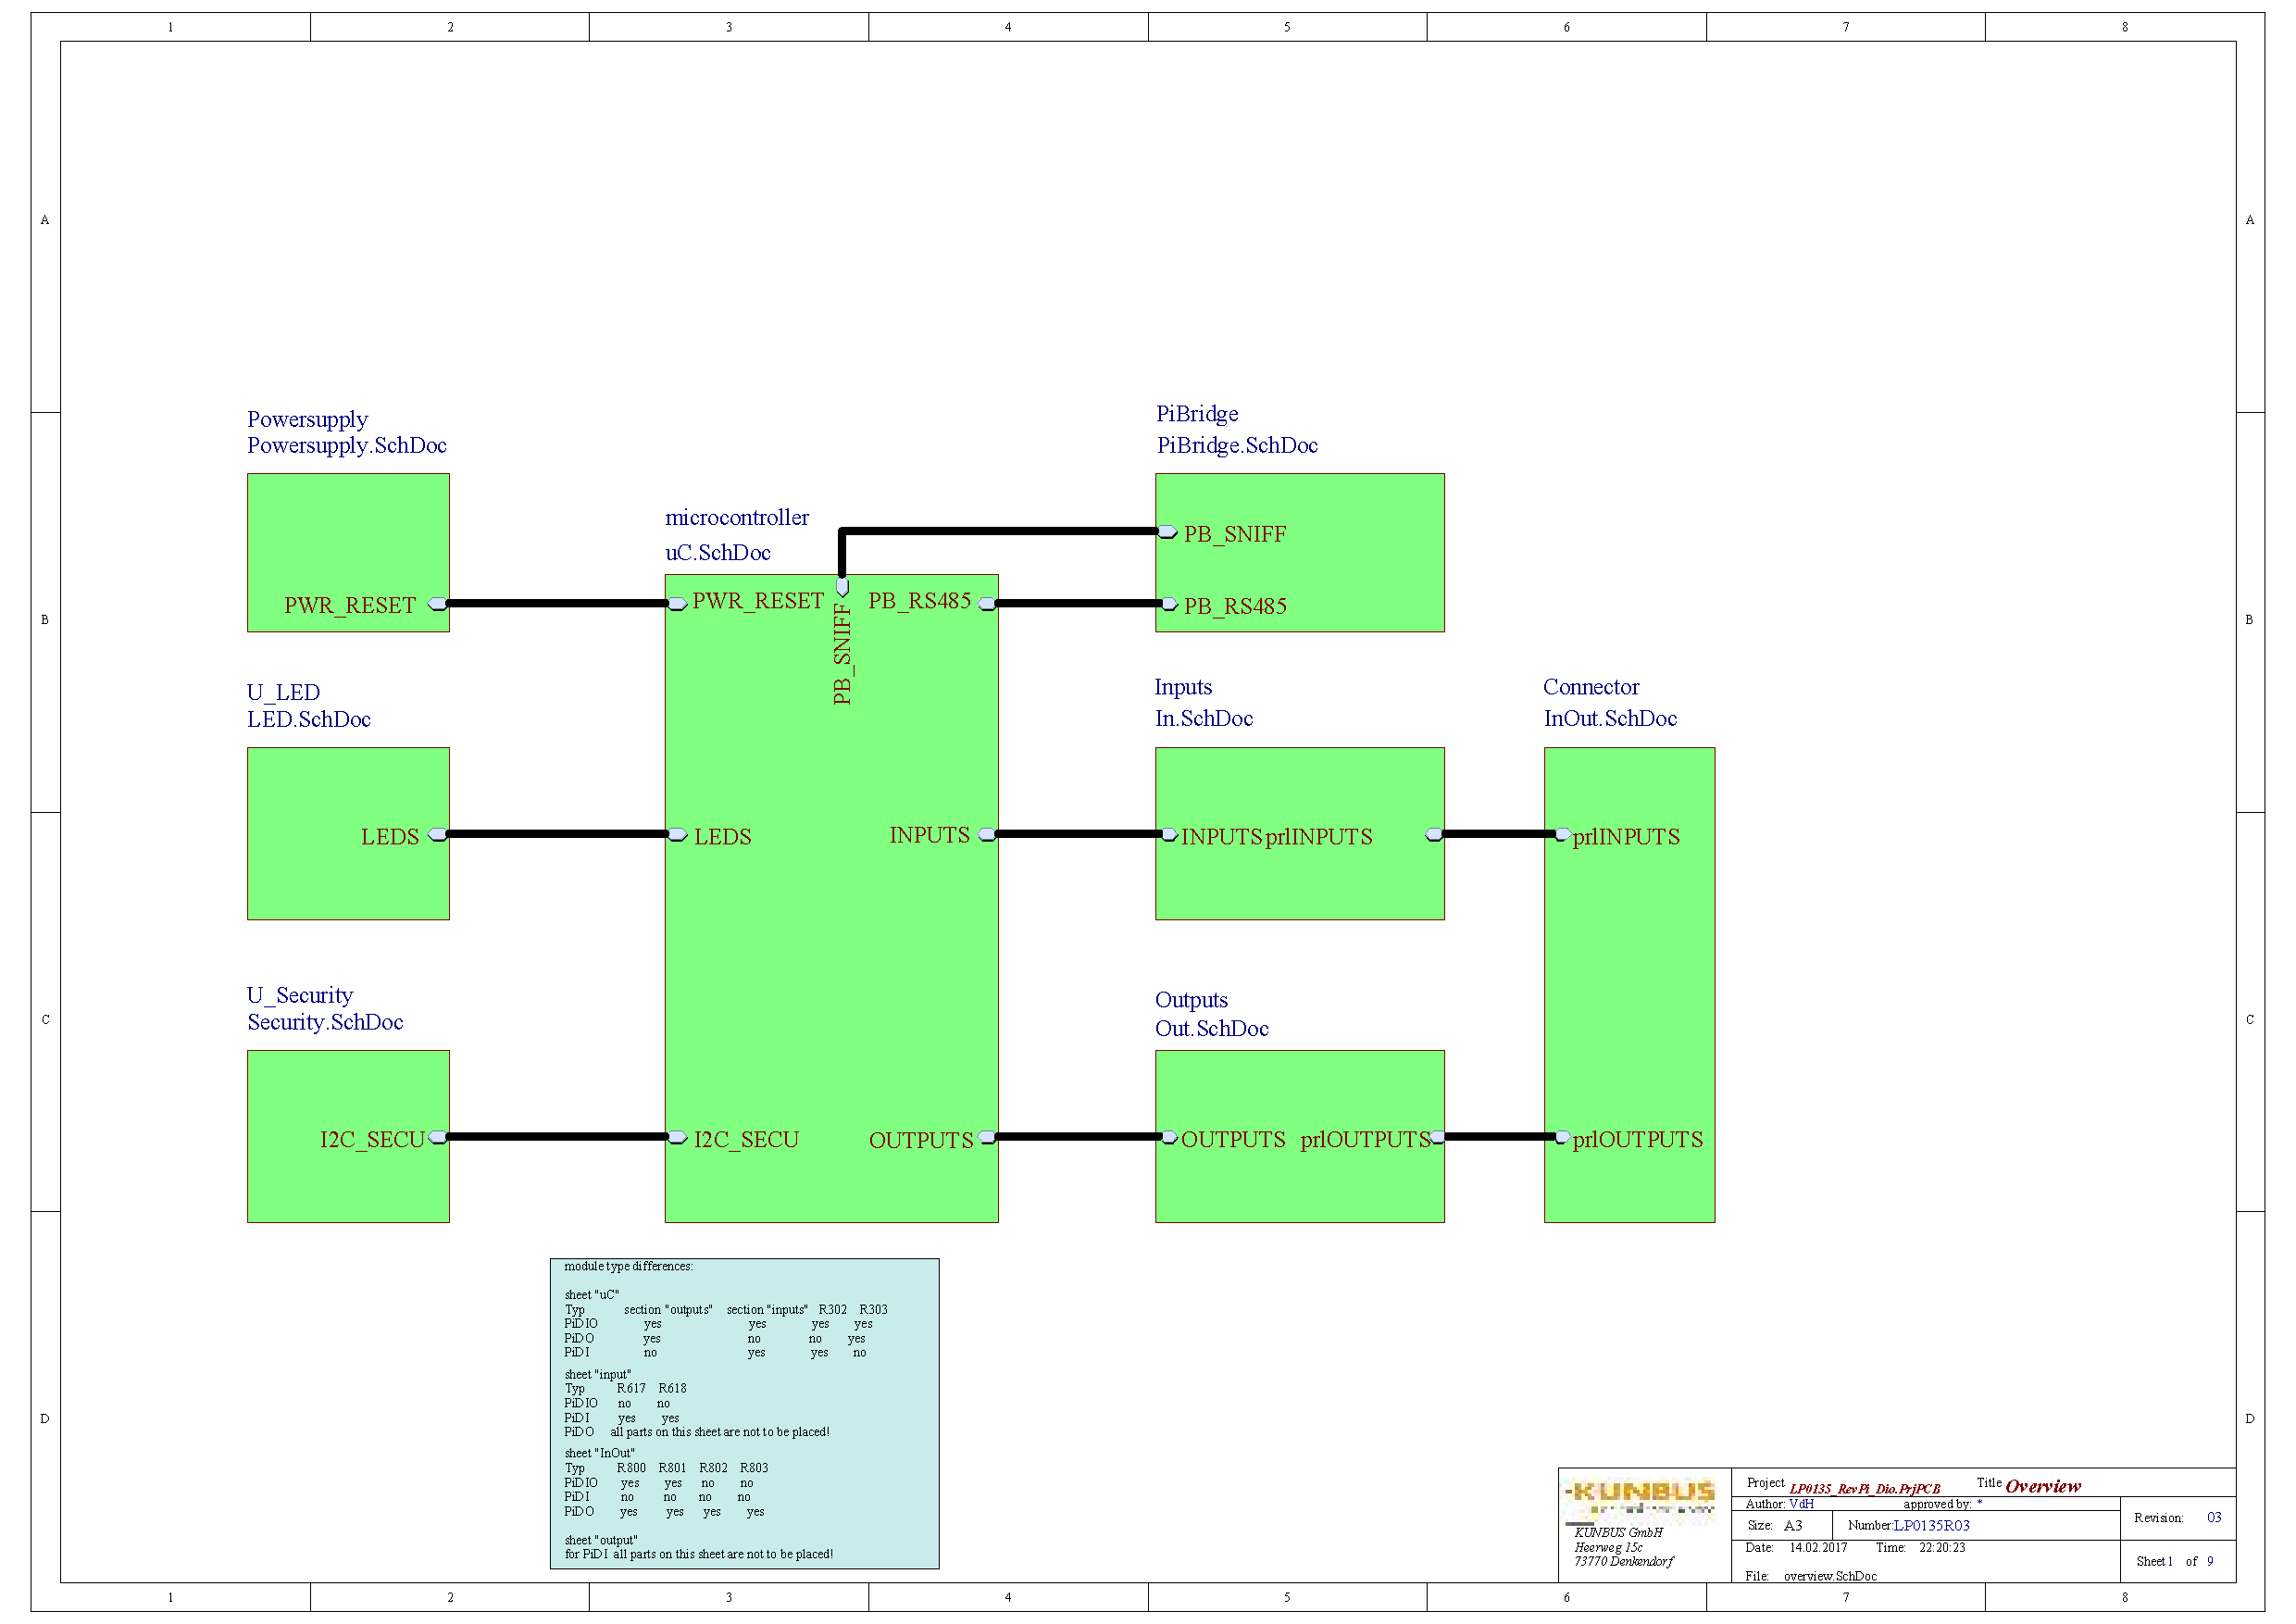
\includegraphics[trim={4cm 7cm 10.5cm 7.3cm}, clip, width=\textwidth]{literature/SchematicPrintsRevPi-DIO}
    \caption{Schematische Darstellung eines DIO-Moduls (Quelle: Kunbus\textsuperscript{\ref{downloads}})
      \label{fig:dio}}
\end{figure}

Jedes der IO-Module stellt ein eigenständiges eingebettetes System dar. Es verfügt
über einen Microcontroller, welcher die IOs bereitstellt und über einen RS485-Bus
mit dem Revolution Pi kommuniziert (siehe Bild~\ref{fig:dio}). 
Kunbus stellt exemplarisch den Quellcode eines DIO-Moduls unter der MIT Lizenz zur
Verfügung\footnote{\url{https://github.com/RevolutionPi/IODeviceExample}}. 


\subsection{Echtzeit und Multitasking unter Linux -- preemptRT und posix%
     \label{sec:2-echtzeit}}
     
Moderne Betriebssysteme realisieren Multitasking i.d.R.\,in Form des präemptiven Multitasking. 
Der Kernel verfügt über einen sog. Scheduler. Dieser priorisiert alle Prozesse und weist ihnen 
Rechenzeit in sog. Time Slots zu. Die Größe der Zeitfenster sowie die Ausführungsreihenfolge 
ist von der Priorität eines Prozesses abhängig. Besonders an einem präemptiven im Gegensatz zu einem kooperativen Scheduler ist dessen Fähigkeit, Tasks während ihrer Ausführung zu unterbrechen bzw. zu pausieren, wenn diese eine bestimmte Dauer überschreiten oder ein höher priorisierter Prozess (bspw. ausgelöst durch einen Interrupt oder durch eine inhärente Periodizität) Rechenleistung benötigt.

Eine Sonderform des präemptiven Multitasking ist das präemptible Multitasking. Hierbei werden auch Teile 
des Kernels als Threads durch den Scheduler ausgeführt. Dieser ist somit in der Lage, auch Prozesse des Kernels
zu unterbrechen, wenn andere Anwendungen Prozessorzeit oder Zugriff auf andere Systemressourcen benötigen
\citep[vgl.][]{web-wiki-praempt}.
     
Der Linux-Kernel implementiert unterschiedliche Präemptions-Modelle \citep[vgl.][/preemption\_models]{web-linuxwiki-basics}:

\begin{itemize}
  \item No Forced Preemption (server):
  Ausgelegt auf maximal möglichen Durchsatz, lediglich Interrupts und
  System-Call-Returns bewirken Präemption.

  \item Voluntary Kernel Preemption (Desktop):
  Neben den implizit bevorrechtigten Interrupts und System-Call-Returns gibt es
  in diesem Modell weitere Abschnitte des Kernels in welchen Preämption explizit
  gestattet ist.

  \item Preemptible Kernel (Low-Latency Desktop):
  In diesem Modell ist der gesamte Kernel, mit Ausnahme sog.~kritischer Abschnitte
  präemptible. Nach jedem kritischen Abschnitt gibt es einen impliziten Präemptions-Punkt.

  \item Preemptible Kernel (Basic RT):
  Dieses Modell ist dem zuvor genannten sehr ähnlich, hier sind jedoch alle Interrupt-Handler
  als eigenständige Threads ausgeführt.

  \item Fully Preemptible Kernel (RT):
  Wie auch bei den beiden zuvor genannten Modellen ist hier der gesamte Kernel
  präemtible. Die Anzahl und Dauer der nicht-präemtiblen kritischen Abschnitte
  ist auf ein notwendiges Minimum beschränkt. Alle Interrupt-Handler sind als
  eigenständige Threads ausgeführt, Spinlocks durch Sleeping-Spinlocks und Mutexe
  durch sog.~RT-Mutexe ersetzt.

\end{itemize}

Lediglich ein präemtibler Kernel kann hartes Echtzeit-Verhalten realisieren, 
da nur hier eine maximale Antwortzeit garantiert werden kann.
Viele Prozesse in der Automatisierungstechnik erfordern harte Echtzeit. 
Eine verspätete Antwort auf eine Anfrage, 
wie etwa das Signal eines Lagenendschalters oder eines Notausschalters kann hier nicht nur über
den Erfolg eines Prozesses, sondern auch über das Leben der daran beteiligten Mitarbeiter entscheiden.
Für weiterführende Erklärungen bzgl.\,Echtzeit, Mutexen und 
Spinlocks sei an dieser Stelle auf die Vorlesung verwiesen~\citep{script-peter}.


\subsubsection{preemptRT%
        \label{sec:2-preemptRT}}

Der Kernel des auf dem Revolution Pi installierten Raspbian mit PREEMP\_RT Patch fällt 
in die Kategorie des \glqq{}Fully Preemptible Kernels\grqq{} (siehe Abschnitt \ref{sec:2-echtzeit}).
Das zugrunde liegende Prinzip lässt sich wie folgt formulieren: Nur Code, welcher absolut nicht-präemtible sein darf, ist es
gestattet nicht-präemtible zu sein. Ziel ist folglich, die Menge des nicht-präemtiblen 
Codes im Linux-Kernel auf das absolut notwendige Minimum zu reduzieren.

Dies wird durch Verwendung folgender Mechanismen erreicht~\citep[vgl.][]{web-linuxwiki-details}:

\begin{itemize}
  \item Hochauflösende Timer
  \item Sleeping Spinlocks
  \item Threaded Interrupt Handlers
  \item rt\_mutex
  \item RCU
\end{itemize}

Diese Mechanismen sind bspw. im Linux-Wiki\footnote{siehe \url{https://wiki.linuxfoundation.org/realtime/documentation/technical_details}} ausführlich beschrieben.

\subsubsection{POSIX%
        \label{sec:2-posix}}
Das Portable Operating System Interface (POSIX) bezeichnet eine Sammlung von Standards, 
welche auf dem Unix-System basieren, jedoch nicht auf dieses beschränkt sind.

Der Wechsel zwischen verschiedenen Unix-Distributionen brachte oft Kompatibilitätsprobleme mit sich. 
Dieser Mangel an Portabilität erschwerte Benutzern und Entwicklern die Verwendung bzw. Bereitstellung 
von Software auf unterschiedlichen Systemen. 
Das Institut für Elektrotechnik und Elektronik (IEEE) begann 1984 mit der Entwicklung des Unix-Standards.
Sie entwickelten das, was heute als Single UNIX Specification bekannt ist und allgemein als POSIX bezeichnet wird~\citep[vgl.][]{web-debianwiki-posix}.
Das Konsortium \glqq{}The Open Group\grqq{} überwacht die weitere Entwicklung dieses Standards.
Ferner stellt es einen Teil der POSIX-Spezifikation frei zur Verfügung~\citep[vgl.][]{web-opengroup-posix}.

Die aktuelle Version POSIX.1-2017 ist verfügbar als IEEE Standard 1003.1-2017 sowie in Form der \glqq{}The Open Group Technical Standard Base Specifications\grqq{}, Ausgabe 7. POSIX.1-2017 definiert eine Standard-Betriebssystemschnittstelle und -umgebung, einschließlich eines Befehlsinterpreters (auch Shell genannt) und gängiger Dienstprogramme zur Unterstützung der Portabilität von Anwendungen auf Quellcode-Ebene. POSIX.1-2017 ist sowohl für Anwendungsentwickler als auch für Systemimplementierer gedacht und umfasst vier Hauptkomponenten \citep[vgl.][]{web-opengroup-overview}:
\begin{itemize}
    \item Basisdefinitionen:\\
          Allgemeine Begriffe, Konzepte und Schnittstellen einschließlich Hilfskonventionen und C-Headern
          
    \item Systemschnittstellen:\\
          Definitionen für Systemdienstfunktionen und Unterprogramme, C-spezifische Systemdienste, Portabilität
        
    \item Shell und Dienstprogramme:\\
          Definitionen für eine Schnittstelle zur Befehlsinterpretation von Diensten und gängige Hilfsprogramme
    
    \item Begründungen und Historie
\end{itemize}

Debian basiert auf Linux und verwendet den Linux-Kernel. Linux ist zu großen Teilen POSIX-kompatibel. Debian ist jedoch nicht POSIX-zertifiziert, da diese Zertifizierung mit hohen Kosten verbunden ist\citep[vgl.][Kapitel 4.4.]{web-debian-faq}.

Beide Kernkomponenten des in dieser Arbeit vorgestellten Projektes nutzen Komponenten von Linux, 
welche an den POSIX-Standard angelehnt sind: open62541 verwendet u.a.\,POSIX-Threads und
Mutexe~\citep[vgl.][pthread.h]{web-opengroup-pthread}, piControl nutzt POSIX-Semaphoren
\citep[vgl.][semaphore.h]{web-opengroup-semaphore}. 


\subsection{OPC-UA und open62541%
     \label{sec:2-opc}}
In diesem Abschnitt sollen Möglichkeiten des Datenaustausch zwischen Komponenten der
Automatisierungstechnik vorgestellt werden. OPC-UA stellt einen offenen, IP-basierten Kommunikationsstandard
für Sensoren und Steuerungen dar. open62541 ist eine freie Client- sowie Server-Implementierung dieses
Standards, geschrieben in C.


\subsubsection{OPC UA%
        \label{sec:2-opcua}}

Open Platform Communications (OPC) ist eine Familie von Standards zur herstellerunabhängigen
Kommunikation von Maschinen (M2M) in der Automatisierungstechnik. Die sog. OPC Task Force, zu deren
Mitgliedern verschiedene etablierte Firmen der Automatisierungsindustrie gehören, veröffentlichte
die OPC Specification Version 1.0 im August 1996.
Motiviert ist dieser offene Standard durch die Erkenntniss, dass die Anpassung der
zahlreichen Herstellerstandards an individuelle Infrastrukturen und Anlagen einen
großen Mehraufwand verursachen.
Die Wikipedia beschreibt das Anwendungsgebiet für OPC wie folgt \citep[vgl.][]{web-wiki-opc}:

\glqq{}OPC wird dort eingesetzt, wo Sensoren, Regler und Steuerungen verschiedener Hersteller
ein gemeinsames Netzwerk bilden. Ohne OPC benötigten zwei Geräte zum Datenaustausch
genaue Kenntnis über die Kommunikationsmöglichkeiten des Gegenübers. Erweiterungen
und Austausch gestalten sich entsprechend schwierig. Mit OPC genügt es, für jedes
Gerät genau einmal einen OPC-konformen Treiber zu schreiben. Idealerweise wird
dieser bereits vom Hersteller zur Verfügung gestellt. Ein OPC-Treiber lässt sich
ohne großen Anpassungsaufwand in beliebig große Steuer- und Überwachungssysteme
integrieren.

OPC unterteilt sich in verschiedene Unterstandards, die für den jeweiligen Anwendungsfall
unabhängig voneinander implementiert werden können. OPC lässt sich damit verwenden
für Echtzeitdaten (Überwachung), Datenarchivierung, Alarm-Meldungen und neuerdings
auch direkt zur Steuerung (Befehlsübermittlung).\grqq{}

OPC basiert in der ursprünglichen Spezifikation (auch als OPC DA bezeichnet) auf Microsofts DCOM-Spezifikation.
DCOM macht Funktionen und Objekte einer Anwendung anderen Anwendungen im Netzwerk
zugänglich. Der OPC-Standard definiert entsprechende DCOM-Objekte um mit anderen
OPC-Anwendungen Daten austauschen zu können. Die Verwendung von DCOM bindet Anwender
jedoch an Betriebssysteme von Microsoft. 

\begin{figure}
    \centering
    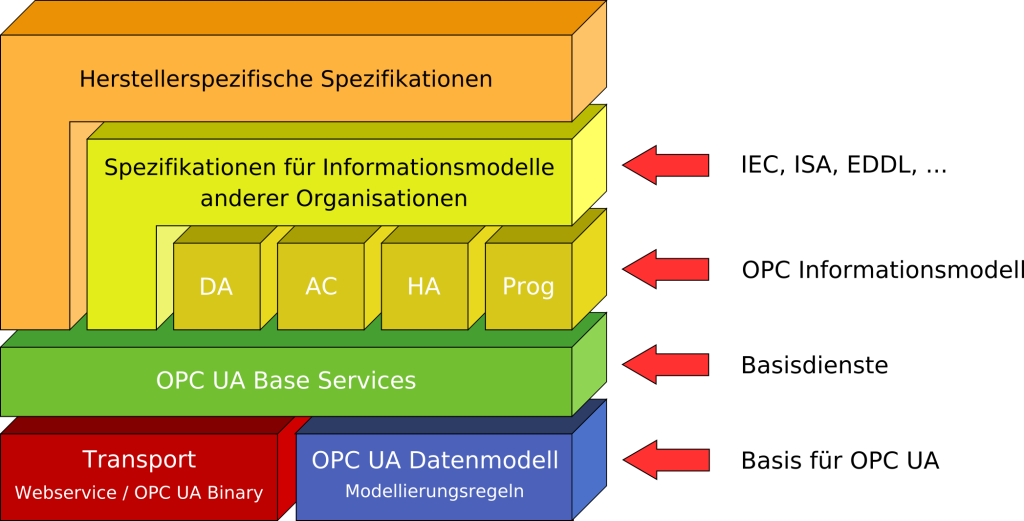
\includegraphics[width=0.85\textwidth]{images/UA_Architecture_1024.png}
    \caption{Die OPC Unified Architecture. Grafik von Gerhard Gappmeier - ascolab GmbH, CC BY-SA 3.0}
    \label{fig:opc-unified-architecture}
\end{figure}
% Evtl Grafik: Von Gerhard Gappmeier - ascolab GmbH, CC BY-SA 3.0, https://de.wikipedia.org/w/index.php?curid=1892069

Die ursprüngliche OPC Spezifikation wurde 2006 durch die Entwicklung der 
OPC Unified Architecture (OPC UA) überholt. 
Diese zeichnet sich durch eine Service-orientierte Architektur (SOA) aus, deren Struktur
aus mehreren Schichten besteht, siehe Abbilung~\ref{fig:opc-unified-architecture}. 
Über der untersten Schicht, dem Betriebssystem des Servers, verbindet eine Portabilitäts-Schicht 
den sog.\, UA ANSI C Stack mit einer API. Diese API kann bspw.\,in C++ geschrieben sein, 
und erlaubt die Anbindung der obersten Schicht, der Anwendungsschicht~\citep[vgl.][]{web-spec-opc}.
OPC UA setzt auf einem eigenen Kommunikationsstack auf; die Verwendung von DCOM
und damit die Bindung an Microsoft wurden aufgelöst.

Neben Architektur und Kommunikationsschnittstellen wird in der OPC Spezifikation auch ein 
Informationsmodell definiert. Die deutschsprachige Wikipedia beschreibt dieses wie folgt: 

\glqq{}Das OPC[-UA]-Informationsmodell ist nicht mehr nur eine Hierarchie aus Ordnern, Items
und Properties. Es ist ein sogenanntes Full-Mesh-Network aus Nodes, mit dem neben
den Nutzdaten eines Nodes auch Meta- und Diagnoseinformationen repräsentiert werden. [...]
Ein Node ähnelt einem Objekt aus der objektorientierten Programmierung. Ein Node
kann Attribute besitzen, die gelesen werden können. Es ist möglich Methoden zu definieren und aufzurufen. [...]
Weiterhin werden Events unterstützt, die versendet werden können
(AE (Alarms \& Events), DA DataChange), um bestimmte Informationen zwischen Geräten
auszutauschen. Ein Event besitzt unter anderem einen Empfangszeitpunkt, eine Nachricht
und einen Schweregrad. Die o.\,g. Nodes werden sowohl für die Nutzdaten als auch
alle anderen Arten von Metadaten verwendet. Der damit modellierte OPC-Adressraum
beinhaltet nun auch ein Typmodell, mit dem sämtliche Datentypen spezifiziert werden.\grqq{}


\subsubsection{open62541%
        \label{sec:2-open62541}}
open62541 ist eine offene und freie Implementierung von OPC UA. 
Die in C geschriebene Bibliothek stellt eine beständig zunehmende Anzahl der im OPC UA Standard definierten
Funktionen bereit. Sie kann sowohl zur Erstellung von OPC-Servern als auch von -Clients
genutzt werden. Ergänzend zu der unter der Mozilla Public License v2.0 lizensierten
Bibliothek stellt das open62541 Projekt auch Beispielprogramme unter einer CC0 Lizenz
zur Verfügung.
Zu den Unterstützern des Projektes zählen u.a.\, die RWTH Aachen, das Frauenhofer IOSB sowie die TU Dresden.

Die Bibliothek eignet sich auch für die Entwicklung auf eingebetteten Systemen und
Microcontrollern. Die Größe einer Server-Binary kann weniger als 100kB betragen.

Folgende Auswahl an Eigenschaften und Funktionen zeichnet die in dieser Arbeit verwendete
Version 0.3 von open62541 aus:
\begin{itemize}
  \item Kommunikationionsstack
  \begin{itemize}
      \item OPC UA Binär-Protokoll (HTTP oder SOAP werden gegenwärtig nicht unterstützt)
      \item Austauschbare Netzwerk-Schicht, welche die Verwendung eigener Netzwerk-APIs
      erlaubt.
      \item Verschlüsselte Kommunikationion
      \item Asynchrone Dienst-Anfragen im Client
  \end{itemize}
  \item Informationsmodell
  \begin{itemize}
    \item Unterstützung aller OPC UA Node-Typen, inkl.~Methoden
    \item Hinzufügen und Entfernen von Nodes und Referenzen zur Laufzeit.
    \item Vererbung und Instanziierung von Objekt- und Variablentypen
    \item Zugriffskontrolle auch für einzelne Nodes
  \end{itemize}
  \item Subscriptions
  \begin{itemize}
    \item Erlaubt die Überwachung (subscriptions / monitoreditems)
    \item Sehr geringer Ressourcenbedarf pro überwachtem Wert
  \end{itemize}
  \item Code-Generierung auf XML-Basis
  \begin{itemize}
    \item Erlaubt die Erstellung von Datentypen
    \item Erlaubt die Generierung des serverseitigen Informationsmodells
  \end{itemize}
\end{itemize}

Weiterführende Informationen und Code-Beispiele bietet die ausführliche Dokumentation des Projektes~\citep[siehe]{web-open62541} sowie der kommentierte Quelltext.

% % % Imports nur für Referenzenauflösung während des Schreibens! Vorm Kompilieren auskommentieren!
% \bibliography{0_hauptdatei}
% \input{1_einleitung}
% \input{2_grundlagen}
% \input{3_konzeption}
% \input{4_implementierung}
% \input{5_tests}
% \input{6_zusammenfassung}
% \input{anhang}
% % Ende Imports

\section{Systemkonzept%
  \label{sec:3-konzeption}}
Auf Basis der in Abschnitt [...] vorgestellten Möglichkeiten folgt nun die Ausarbeitung eines Konzepts.

\subsection{Anbindung der IO an den OPC-Server%
     \label{sec:3-anbindung}}

\subsection{Integration des OPC-Servers in das System%
     \label{sec:3-integration}}

% % % Imports nur für Referenzenauflösung während des Schreibens! Vorm Kompilieren auskommentieren!
% \bibliography{0_hauptdatei}
% \input{1_einleitung}
% \input{2_grundlagen}
% \input{3_konzeption}
% \input{4_implementierung}
% \input{5_tests}
% \input{6_zusammenfassung}
% \input{anhang}
% % Ende Imports

\section{Implementierung%
  \label{sec:4-implementierung}}
Das folgende Kapitel stellt in Auszügen die Implementierung des OPC-Servers sowie die Anbindung an die IO-Module
der SPS dar. Der Schwerpunkt liegt hierbei auf der Funktionsweise des piControl-Treibers und dessen Integration in das Projekt. Abschnitt~\ref{sec:4-picontrol} erklärt die zum Schreibens eines Bits verwendeten Funktionsaufrufe.
Zuvor soll jedoch in Abschnitt~\ref{sec:4-open62541} der Teil des OPC-Servers vorgestellt werden, welcher auf besagten Treiber zugreift. 

\subsection{Implementierung des OPC-Servers%
     \label{sec:4-open62541}}
Wie im vorangegangenen Abschnitt~\ref{sec:3-integration} begründet, soll die Verknüpfung zwischen dem Prozessabbild der SPS und den auf dem OPC-Server bereitgestellten Werten über sog.\,Datenquellen erfolgen. Hierzu ist zunächst eine Callback-Methode zu implementieren, welche bei einem Lese- oder Schreibzugriff auf eine Variable aufgerufen wird. Die Verknüpfung zwischen Callback-Methode und Variable muss manuell erfolgen.

\begin{lstlisting}[language={c},firstnumber=237,caption={Auszug der Methode \lstinline{linkDataSourceVariable} in \lstinline{variables.c}\label{lst:4-linkDataSourceVariable}}]
extern UA_StatusCode
 linkDataSourceVariable(UA_Server *server, UA_NodeId nodeId) {
     bool readonly = false;
     UA_DataSource dataSourceVariable;
     UA_StatusCode rc; |>\setcounter{lstnumber}{254}<|

     dataSourceVariable.read = readDataSourceVariable;
     if (!readonly)
        dataSourceVariable.write = writeDataSourceVariable;
     else
        dataSourceVariable.write = writeReadonlyDataSourceVariable;

     return UA_Server_setVariableNode_dataSource(server, nodeId, dataSourceVariable);
 }
\end{lstlisting}

\begin{figure}[h]
    \centering
    \includegraphics[width=0.42\textwidth]{doc/img/OPC_RevPiDO.pdf}
    \caption{Auszug des verwendeten Nodesets, hier Digitalausgang 1 des Versuchsaufbaus
      \label{fig:opc-do}}
\end{figure}

Die in Listing~\ref{lst:4-linkDataSourceVariable} abgebildete Methode \lstinline{linkDataSourceVariable()} erzeugt ein Struct vom Typ \lstinline{UA_DataSource}. In diesem werden dem Lesen und Schreiben einer OPC-Variablen entsprechende Callback-Methoden zugewiesen. Die Verknüpfung einer OPC-Variable, genauer ihrer NodeId, mit der zuvor definierten Datenquelle erfolgt über die von open62541 bereitgestellte Methode \lstinline{UA_Server_setVariableNode_dataSource()}. Vor dem Lesen und nach dem Schreiben dieser Variable werden von nun an die entsprechenden Callbacks aufgerufen.
     
\begin{lstlisting}[language={c},firstnumber=168,caption={Auszug des Callbacks \lstinline{writeDataSourceVariable} in \lstinline{variables.c}\label{lst:4-writeDataSourceVariable}}]  
extern UA_StatusCode
 writeDataSourceVariable(UA_Server *server,
            const UA_NodeId *sessionId, void *sessionContext,
            const UA_NodeId *nodeId, void *nodeContext,
            const UA_NumericRange *range, const UA_DataValue *dataValue) {

    UA_StatusCode retval  = UA_STATUSCODE_GOOD;
    UA_NodeId *nameNodeId = UA_malloc(sizeof(UA_NodeId));
    UA_QualifiedName nameQN = UA_QUALIFIEDNAME(1, "Name");
    UA_Variant nameVar;
    UA_Boolean bit;

    retval |= findSiblingByBrowsename(server, nodeId, &nameQN, nameNodeId);
    retval |= UA_Server_readValue(server, *nameNodeId, &nameVar);
    retval |= UA_Boolean_copy(dataValue->value.data, &bit);

    |>\tikzmarkin[set border color=martinired]{writeIO}<|PI_writeSingleIO(String_fromUA_String(nameVar.data), &bit, false);                                                 |>\tikzmarkend{writeIO}<|

    free(nameNodeId);
    return retval;
 }
\end{lstlisting}

Listing~\ref{lst:4-writeDataSourceVariable} zeigt die Callback-Methode, welche nach dem Schreiben einer Variablen auf dem OPC-Server aufgerufen wird.
Dieser Methode wird neben der NodeId der mit ihr verknüpften Variablen auch der Wert dieser in Form eines Zeigers auf ein Struct vom Typ \lstinline{UA_DataValue} übergeben.

Die Gestaltung des hier verwendeten Nodesets sieht vor, dass in einer OPC-Variablen \lstinline{"Name"} der Bezeichner des zu schreibenden Digitalausgangs hinterlegt ist, siehe Abbildung~\ref{fig:opc-do}. Dies erlaubt eine Rekonfiguration der Ein- und Ausgänge der SPS ohne Änderungen im Programmcode des OPC-Servers vornehmen zu müssen.
Es ist daher erforderlich, nach jedem Schreiben einer mit einem Digitalausgang verknüpften Variablen, hier \lstinline{"Value"}, dessen Bezeichner \lstinline{"Name"} abzufragen. 
Dies geschieht in den Zeilen 180 und 181.
Anschließend wird dieser Bezeichner sowie der zu schreibende Wert der Methode \lstinline{PI_writeSingleIO()} übergeben, welche wiederum die Interaktion mit piControl übernimmt (vgl. Abschnitt \ref{sec:4-picontrol}).
 
\subsection{Integration von piControl%
     \label{sec:4-picontrol}}
In Abschnitt~\ref{sec:2-io} wurde die Anbindung der IO-Module des Revolution Pi sowie die Funktionsweise von piControl aus Anwendersicht beschrieben. Die verfügbare Literatur beschränkt sich auch auf lediglich diese Sicht; eine weiterführende Dokumentation für Entwickler gibt es, neben der in Abschnitt~\ref{sec:3-anbindung} vorgestellten Manpage, nicht. 
In diesem Abschnitt soll daher der Quellcode von piControl sowie dessen Verwendung im Projekt genauer betrachtet werden.
Hierzu wird exemplarisch die in Abschnitt~\ref{sec:4-open62541} eingeführte Methode \lstinline{PI_writeSingleIO()} untersucht.
Diese Methode ermöglicht das Setzen eines einzelnen Bits im Prozessabbild der SPS, und damit das Schalten eines digitalen Ausgangs auf einem IO-Modul.
Die äquivalente Methode \lstinline{int piControlGetBitValue(SPIValue *pSpiValue)} zum Lesen eines Bits bzw. Eingangs funktioniert analog und soll daher an dieser Stelle nicht dediziert erörtert werden.

\begin{lstlisting}[language={c},firstnumber=97,
                   caption={Setzen eines phsikalischen, digitalen Ausgangs in \lstinline{revpi.c}
                   \label{lst:4-PI_writeSingleIO}}]
extern void PI_writeSingleIO(char *pszVariableName, bool *bit, bool verbose)
{
	int rc;
	SPIVariable sPiVariable;
	SPIValue sPIValue;

	strncpy(sPiVariable.strVarName, pszVariableName, sizeof(sPiVariable.strVarName));
	rc = piControlGetVariableInfo(&sPiVariable);
	if (rc < 0) {
		printf("Cannot find variable '%s'\n", pszVariableName);
		return;
	}

		sPIValue.i16uAddress = sPiVariable.i16uAddress;
		sPIValue.i8uBit = sPiVariable.i8uBit;
		sPIValue.i8uValue = *bit;
		rc = |>\tikzmarkin[set border color=martinired]{setBitValue}<|piControlSetBitValue(&sPIValue)|>\tikzmarkend{setBitValue}<|;
		if (rc < 0)
			printf("Set bit error %s\n", getWriteError(rc));
		else if (verbose)
			printf("Set bit %d on byte at offset %d. Value %d\n", sPIValue.i8uBit, sPIValue.i16uAddress,
			       sPIValue.i8uValue);
}
\end{lstlisting}

Der Programmcode in Listing~\ref{lst:4-PI_writeSingleIO} ist Teil des implementierten OPC-Servers. In diesem wird auf zwei Funktionen des piControl-Treibers zugegriffen. 
Beiden Methoden wird als Argument ein Zeiger auf ein Struct vom Typ \lstinline{SPIValue} übergeben. Der im Struct abgelegte Name wird mittels \lstinline{piControlGetVariableInfo(&sPIValue)} zu einer Adresse im Prozessabbild aufgelöst. Diese wird in \lstinline{sPIValue.i16uAdress} gespeichert. Der Wert der Variablen wird anschließend mittels \lstinline{piControlSetBitValue(&sPIValue)} an dieser Adresse in das Prozessabbild geschrieben.

\begin{lstlisting}[language={c},firstnumber=309,caption={Methode \lstinline{piControlSetBitValue} in \lstinline{piControlIf.c}\label{lst:4-piControlSetBitValue}}]
int |>\tikzmarkin[set border color=martiniblue]{setBitValueFcn}<|piControlSetBitValue(SPIValue *pSpiValue)|>\tikzmarkend{setBitValueFcn}<|
{
    piControlOpen();

    if (PiControlHandle_g < 0)
	    return -ENODEV;

    pSpiValue->i16uAddress += pSpiValue->i8uBit / 8;
    pSpiValue->i8uBit %= 8;

    if (|>\tikzmarkin[set border color=martinired]{ioctl}<|ioctl(PiControlHandle_g, KB_SET_VALUE, pSpiValue)|>\tikzmarkend{ioctl}<| < 0)
	    return errno;

    return 0;
}
\end{lstlisting}

Die in Listing~\ref{lst:4-piControlSetBitValue} dargestellte Methode \lstinline{piControlSetBitValue} ist lediglich eine Hüllfunktion (häufig auch als Wrapper-Funktion bezeichnet) für einen Aufruf des \lstinline{ioctl} Kernel-Moduls.
Folgende Parameter werden übergeben:
\lstinline{PiControlHandle_g} ist die Referenz auf die Geräte-Datei des piControl-Treibers. \lstinline{KB_SET_VALUE} ist das ioctl-Kommando zum Schreiben eines Bits in das Prozessabbild. Der Zeiger \lstinline{pSpiValue} verweist auf ein Struct des bereits vorgestellten Typs \lstinline{SPIValue}.

\begin{lstlisting}[language={c},firstnumber=80,caption={Methode \lstinline{piControlOpen} in \lstinline{piControlIf.c}\label{lst:4-piControlOpen}}]
void piControlOpen(void)
{
    /* open handle if needed */
    if (PiControlHandle_g < 0)
    {
	    |>\tikzmarkin[set border color=martiniblue]{PiControlHandle}<|PiControlHandle_g = open(PICONTROL_DEVICE, O_RDWR)|>\tikzmarkend{PiControlHandle}<|;
    }
}
\end{lstlisting}

Die in Listing~\ref{lst:4-piControlOpen} dargestellte Methode öffnet, sofern nicht bereits geschehen, die Geräte-Datei. Das Macro \lstinline{PICONTROL_DEVICE} verweist hierbei auf \lstinline{/dev/piControl0}.

\begin{lstlisting}[language={c},firstnumber=721,caption={Methode \lstinline{piControlIoctl} in \lstinline{piControlMain.c}\label{lst:4-piControlIoctl}}]
static long |>\tikzmarkin[set border color=martiniblue, below offset=0.9em]{piControlIoctl}<|piControlIoctl(struct file *file, unsigned int prg_nr, 
                           unsigned long usr_addr)                                      |>\tikzmarkend{piControlIoctl}<|
{
  int status = -EFAULT;
  tpiControlInst *priv;
  int timeout = 10000;	// ms

  if (prg_nr != KB_CONFIG_SEND && prg_nr != KB_CONFIG_START && !isRunning()) {
  	return -EAGAIN;
  }

  priv = (tpiControlInst *) file->private_data;

  if (prg_nr != KB_GET_LAST_MESSAGE) {
  	// clear old message
  	priv->pcErrorMessage[0] = 0;
  }

  switch (prg_nr) {|>\setcounter{lstnumber}{864}<|

    case |>\tikzmarkin[set border color=martiniblue]{KB_SET_VALUE}<|KB_SET_VALUE:|>\tikzmarkend{KB_SET_VALUE}<|
  		{
  			SPIValue *pValue = (SPIValue *) usr_addr;

  			if (!isRunning())
  				return -EFAULT;

  			if (pValue->i16uAddress >= KB_PI_LEN) {
  				status = -EFAULT;
  			} else {
  				INT8U i8uValue_l;
  				my_rt_mutex_lock(&piDev_g.lockPI);
  				i8uValue_l = piDev_g.ai8uPI[pValue->i16uAddress];

  				if (pValue->i8uBit >= 8) {
  					i8uValue_l = pValue->i8uValue;
  				} else {
  					if (pValue->i8uValue)
  						i8uValue_l |= (1 << pValue->i8uBit);
  					else
  						i8uValue_l &= ~(1 << pValue->i8uBit);
  				}

  				|>\tikzmarkin[set border color=martinired]{i8uValue}<|piDev_g.ai8uPI[pValue->i16uAddress] = i8uValue_l;|>\tikzmarkend{i8uValue}<|
  				rt_mutex_unlock(&piDev_g.lockPI);

  #ifdef VERBOSE
  				pr_info("piControlIoctl Addr=%u, bit=%u: %02x %02x\n", pValue->i16uAddress, pValue->i8uBit, pValue->i8uValue, i8uValue_l);
  #endif

  				status = 0;
  			}
  		}
  		break; |>\setcounter{lstnumber}{1314}<|

    default:
      pr_err("Invalid Ioctl");
      return (-EINVAL);
      break;

    }

    return status;
  }
\end{lstlisting}

Listing~\ref{lst:4-piControlIoctl} zeigt in Auszügen die ioctl-Methode des piControl Kernel-Treibers. Diese bekommt folgende Argumente übergeben: \lstinline{struct file *file} enthält den Verweis auf die Geräte-Datei, hier \lstinline{/dev/piControl0}. Der Wert von \lstinline{unsigned int prg_nr} beschreibt die Anfrage an den Treiber, in diesem Fall \lstinline{KB_SET_VALUE}. Das Argument \lstinline{unsigned long usr_addr} enthält einen typ-agnostischen Pointer. Dieser verweist auf einen Speicherbereich, in welchem die zur Bearbeitung der Anfrage notwendigen Daten abgelegt sind. Hier können auch vom Treiber empfangene Daten dem Anwendungsprogramm bereitgestellt werden. 

Die switch-case-Anweisung führt die über das Argument \lstinline{prg_nr} spezifizierte Aktion aus. Hier betrachten wir \lstinline{KB_SET_VALUE}:
Zunächst wird in Zeile 868 der übergebene Zeiger \lstinline{usr_addr} mittels explizitem Typecast zu einem Zeiger des Typs \lstinline{SPIValue *} konvertiert. Da dieser auf Daten im Userspace verweist, ist beim Zugriff durch den Kernel-Treiber besondere Vorsicht geboten.
In Zeile 877 wird mittels Mutex das Prozessabbild \lstinline{piDev_g} für den Zugriff durch andere Threads oder Prozesse gesperrt.
\lstinline{my_rt_mutex_lock} verweist hierbei auf die Funktion \lstinline{rt_mutex_lock} aus \lstinline{linux/sched.h}\footnote{Offenbar wurde hier auch eine alternative Implementierung vorgesehen, siehe revpi\_common.h}

In Zeile 889 wird das Byte \lstinline{i8uValue_l}, welches den zu schreibenden Wert enthält in das Prozessabbild übertragen. Anschließend wird die Mutex auf \lstinline{piDev_g} wieder entsperrt.
\newpage

\begin{lstlisting}[language={c},firstnumber=62,caption={Auszug des Struct \lstinline{spiControlDev} in \lstinline{piControlMain.h}\label{lst:4-spiControlDev}}]
|>\tikzmarkin[set border color=martiniblue]{spiControlDev}<|typedef struct spiControlDev|>\tikzmarkend{spiControlDev}<| {
	// device driver stuff
	int init_step;
	enum revpi_machine machine_type;
	void *machine;
	struct cdev cdev;	// Char device structure
	struct device *dev;
	struct thermal_zone_device *thermal_zone;

	|>\tikzmarkin[set border color=martiniblue]{processImage}<|// process image stuff
	INT8U ai8uPI[KB_PI_LEN];
	INT8U ai8uPIDefault|>\tikzmarkin[set border color=martinired]{KB_PI_LEN_0}<|[KB_PI_LEN]|>\tikzmarkend{KB_PI_LEN_0}<|;
	struct rt_mutex lockPI;        |>\tikzmarkend{processImage}<|
	bool stopIO;
	piDevices *devs; |>\setcounter{lstnumber}{94}<|
} tpiControlDev;
\end{lstlisting}

Das Prozessabbild ist als Byte-Array der Länge \lstinline{KB_PI_LEN} in Listing~\ref{lst:4-spiControlDev} definiert. Konfigurationsparameter wie \lstinline{KB_PI_LEN} oder die Zykluszeit für den Datenaustausch zwischen SPS und IO-Modulen sind im folgenden Listing~\ref{lst:4-process} definiert.

\begin{lstlisting}[language={c},firstnumber=119,caption={Konfigurationsparameter des Prozessabbildes in project.h\label{lst:4-process}}]
#define INTERVAL_PI_GATE (5*1000*1000)  // 5 ms piGateCommunication |>\setcounter{lstnumber}{128}<|

#define INTERVAL_IO_COM (5*1000*1000)  // 5 ms piIoComm |>\setcounter{lstnumber}{132}<|

#define KB_PD_LEN       512
|>\tikzmarkin[set border color=martiniblue]{KB_PI_LEN_1}<|#define KB_PI_LEN       4096|>\tikzmarkend{KB_PI_LEN_1}<|
\end{lstlisting}

Das zu setzende Bit wurde zu diesem Zeitpunkt erfolgreich in das Prozessabbild der SPS geschrieben.
Es stellt sich die Frage, wie dieses nun an das IO-Modul kommuniziert wird.
Die Kommunikation mit allen angebundenen Modulen ist ebenfalls Aufgabe des piControl-Treibers.

\begin{lstlisting}[language={c},firstnumber=256,caption={Auszug der Methode \lstinline{piIoThread} in \lstinline{revpi_core.c}\label{lst:4-piIoThread}}]
static int piIoThread(void *data)
{
	//TODO int value = 0;
	ktime_t time;
	ktime_t now;
	s64 tDiff;

	hrtimer_init(&piCore_g.ioTimer, CLOCK_MONOTONIC, HRTIMER_MODE_ABS);
	piCore_g.ioTimer.function = piIoTimer;

	pr_info("piIO thread started\n");

	now = hrtimer_cb_get_time(&piCore_g.ioTimer);

	PiBridgeMaster_Reset();

	while (!kthread_should_stop()) {
		if (|>\tikzmarkin[set border color=martinired]{PiBridgeMaster}<|PiBridgeMaster_Run()|>\tikzmarkend{PiBridgeMaster}<| < 0)
			break;
	}

	RevPiDevice_finish();

	pr_info("piIO exit\n");
	return 0;
}
\end{lstlisting}

Der Kernel-Thread \lstinline{piIoThread} ist verantwortlich für den zyklischen Datenaustausch mit den IO-Modulen. In diesem wird fortlaufend die Methode \lstinline{PiBridgeMaster_Run()} aufgerufen, siehe Listing~\ref{lst:4-piIoThread}.

\begin{lstlisting}[language={c},firstnumber=262,caption={Auszug der Methode \lstinline{PiBridgeMaster_Run(void)} in \lstinline{RevPiDevice.c}\label{lst:4-PiBridgeMaster_Run}}]
int PiBridgeMaster_Run(void)
{
	static kbUT_Timer tTimeoutTimer_s;
	static kbUT_Timer tConfigTimeoutTimer_s;
	static int error_cnt;
	static INT8U last_led;
	static unsigned long last_update;
	int ret = 0;
	int i;

	my_rt_mutex_lock(&piCore_g.lockBridgeState);
	if (piCore_g.eBridgeState != piBridgeStop) {
		switch (eRunStatus_s) { |>\setcounter{lstnumber}{514}<|
		    case enPiBridgeMasterStatus_EndOfConfig:|>\setcounter{lstnumber}{621}<|
		    if (|>\tikzmarkin[set border color=martinired]{RevPiDevice}<|RevPiDevice_run()|>\tikzmarkend{RevPiDevice}<|) {
				// an error occured, check error limits |>\setcounter{lstnumber}{641}<|
			} else {
				ret = 1;
			}
			piCore_g.image.drv.i16uRS485ErrorCnt = RevPiDevice_getErrCnt();
			break;
\end{lstlisting}

Die in Listing~\ref{lst:4-PiBridgeMaster_Run} dargestellte Methode ist eine sog. State-Machine. Ist die Konfiguration der IO-Module erfolgreich abgeschlossen, so führt sie bei Aufruf lediglich die Methode \lstinline{RevPiDevice_run()} aus.

\begin{lstlisting}[language={c},firstnumber=140,caption={Auszug der Methode \lstinline{RevPiDevice_run(void)} in \lstinline{RevPiDevice.c}\label{lst:4-RevPiDevice_run}}]
int RevPiDevice_run(void)
{
	INT8U i8uDevice = 0;
	INT32U r;
	int retval = 0;

	RevPiDevices_s.i16uErrorCnt = 0;

	for (i8uDevice = 0; i8uDevice < RevPiDevice_getDevCnt(); i8uDevice++) {
		if (RevPiDevice_getDev(i8uDevice)->i8uActive) {
			switch (RevPiDevice_getDev(i8uDevice)->sId.i16uModulType) {
			case KUNBUS_FW_DESCR_TYP_PI_DIO_14:
			case KUNBUS_FW_DESCR_TYP_PI_DI_16:
			case KUNBUS_FW_DESCR_TYP_PI_DO_16:
				r = |>\tikzmarkin[set border color=martinired]{sendCyclicTelegram}<|piDIOComm_sendCyclicTelegram(i8uDevice)|>\tikzmarkend{sendCyclicTelegram}\setcounter{lstnumber}{166} <|;

				break; |>\setcounter{lstnumber}{216}<|
			}
		}
	} |>\setcounter{lstnumber}{227}<|
	return retval;
}
\end{lstlisting}

Diese iteriert wie in Listing~\ref{lst:4-RevPiDevice_run} abgebildete durch alle gegenwärtig in der SPS konfigurierten Module. Ist das aktuelle Modul als aktiv markiert, so wird anhand eines sog. Firmware-Descriptors entschieden, welche Methode für die Ansteuerung des Moduls aufzurufen ist.

\begin{lstlisting}[language={c},firstnumber=161,caption={Auszug der Methode \lstinline{piDIOComm_sendCyclicTelegram} in \lstinline{piDIOComm.c}\label{lst:4-sendCyclicTelegram}}]
INT32U piDIOComm_sendCyclicTelegram(INT8U i8uDevice_p)
{
	INT32U i32uRv_l = 0;
	SIOGeneric sRequest_l;
	SIOGeneric sResponse_l;
	INT8U len_l, data_out[18], i, p, data_in[70];
	INT8U i8uAddress;
	int ret; |>\setcounter{lstnumber}{239}<|
	
    |>\tikzmarkin[set border color=martinired]{piIoComm}<|ret = piIoComm_send((INT8U *) & sRequest_l, IOPROTOCOL_HEADER_LENGTH + len_l + 1);  |>\tikzmarkend{piIoComm}\setcounter{lstnumber}{298}<|
}
\end{lstlisting}

Im Falle des hier verwendeten DO-Moduls wird die in Listing~\ref{lst:4-sendCyclicTelegram} abgebildete Methode \lstinline{piDIOComm_sendCyclicTelegram()} aufgerufen. Dieser wird ein Zeiger auf das zu schreibende Gerät übergeben. 
Zunächst wird das Prozessabbild mittels eines proprietären, jedoch im Quellcode offen nachvollziehbaren Protokolls in ein \lstinline{sRequest_l} genanntes Byte-Array umgewandelt. Dieser Schritt ist in Listing~\ref{lst:4-sendCyclicTelegram} nicht abgebildet. Anschließend wird \lstinline{piIoComm_send()} ein Zeiger auf die so generierte Schreib-Anfrage übergeben.

\begin{lstlisting}[language={c},firstnumber=220,caption={Auszug der Methode \lstinline{piIOComm_send} in \lstinline{piIOComm.c}\label{lst:4-piIOComm_send}}]
int piIoComm_send(INT8U * buf_p, INT16U i16uLen_p)
{
	ssize_t write_l = 0;
	INT16U i16uSent_l = 0;|>\setcounter{lstnumber}{249}<|

	while (i16uSent_l < i16uLen_p) {
		write_l = vfs_write(piIoComm_fd_m, buf_p + i16uSent_l, i16uLen_p - i16uSent_l, &piIoComm_fd_m->f_pos);
		if (write_l < 0) {
			pr_info_serial("write error %d\n", (int)write_l);
			return -1;
		} 
		i16uSent_l += write_l;|>\setcounter{lstnumber}{263}<|
	}
	clear();
	vfs_fsync(piIoComm_fd_m, 1);
	return 0;
}
\end{lstlisting}

Listing~\ref{lst:4-piIOComm_send} zeigt die Implementierung von \lstinline{piIoComm_send()}. Diese Methode ist für das Schreiben der oben generierten Anfrage auf die seriellen Schnittstelle verantwortlich. Realisiert wird dies mittels der Methode \lstinline{vfs_write()}. Diese ist in \lstinline{<linux/fs.h>} definiert. Sie ermöglicht das Schreiben einer Datei im Userspace aus dem Kernel heraus. Geschrieben wird hier die Datei mit dem Deskriptor \lstinline{piIoComm_fd_m}.
Da die Funktion \lstinline{vfs_write()} durch andere Kernel-Tasks unterbrochen werden kann, ist nicht gewährleistet, dass die gesamte Anfrage mit nur einem Aufruf geschrieben wird. Die oben abgebildete while-Schleife stellt das vollständige Senden der Anfrage sicher.

\begin{lstlisting}[language={c},firstnumber=157,caption={Auszug der Methode \lstinline{piIOComm_open_serial} in \lstinline{piIOComm.c}\label{lst:4-piIOComm_open_serial}}]
int piIoComm_open_serial(void)
{   |>\setcounter{lstnumber}{167}<|
	struct file *fd;	/* Filedeskriptor */
	struct termios newtio;	/* Schnittstellenoptionen */

	|>\tikzmarkin[set border color=martiniblue]{fd}<|/* Port oeffnen - read/write, kein "controlling tty", 
	    Status von DCD ignorieren */
	fd = filp_open(|>\tikzmarkin[set border color=martinired]{tty}<|REV_PI_TTY_DEVICE|>\tikzmarkend{tty}<|, O_RDWR | O_NOCTTY, 0); |>\setcounter{lstnumber}{208}<|
	
	piIoComm_fd_m = fd;                                                      |>\tikzmarkend{fd}\setcounter{lstnumber}{217}<|

	return 0;
}
\end{lstlisting}

Der zum Schreiben auf die serielle Schnittstelle verwendete Datei-Deskriptor wird von der in Listing~\ref{lst:4-piIOComm_open_serial} abgebildeten Methode \lstinline{piIoComm_open_serial()} generiert. 

\begin{lstlisting}[language={c},firstnumber=45,caption={Definition der seriellen Schnittstelle in \lstinline{piIOComm.h}\label{lst:4-REV_PI_TTY_DEVICE}}]
#define REV_PI_TTY_DEVICE	"/dev/ttyAMA0"
\end{lstlisting}

Das in Listing~\ref{lst:4-REV_PI_TTY_DEVICE} definierte Macro verweist auf eine der seriellen Schnittstellen des RaspberryPi.
Die Implementierung des zugehörigen Schnittstellentreibers soll hier nicht weiter untersucht werden. Somit ist an dieser Stelle die Kette vom Setzen einer Variablen auf dem OPC-Server bis hin zur Aktualisierung des Prozessabbilds der IO-Module geschlossen.

% \begin{lstlisting}[language={c},firstnumber={226},caption={Setzen der Scheduler-Priorität auf SCHED\_FIFO in 
% revpi\_common.c\label{lst:2-sched_priority}}]
% param.sched_priority = ktprio->prio;
% ret = sched_setscheduler(child, SCHED_FIFO, &param);
% \end{lstlisting}
% % % Imports nur für Referenzenauflösung während des Schreibens! Vorm Kompilieren auskommentieren!
% \bibliography{0_hauptdatei}
% \input{1_einleitung}
% \input{2_grundlagen}
% \input{3_konzeption}
% \input{4_implementierung}
% \input{5_tests}
% \input{6_zusammenfassung}
% % Ende Imports

\section{Test des OPC-Servers im Gesamtsystem%
  \label{sec:5-tests}}

% % % Imports nur für Referenzenauflösung während des schreibens! Vorm Kompilieren auskommentieren!
% \bibliography{0_hauptdatei}
% \input{1_einleitung}
% \input{2_grundlagen}
% \input{3_konzeption}
% \input{4_implementierung}
% \input{5_tests}
% \input{6_zusammenfassung}
% % Ende Imports

\section{Zusammenfassung und Ausblick%
  \label{sec:6-fazit}}
Der folgende Abschnitt~\ref{sec:6-zusammenfassung} fasst die gewonnenen Erkenntnisse und den Stand der Implementierung zusammen.
Den Abschluss dieser Arbeit bildet der Ausblick in Abschnitt~\ref{sec:6-ausblick}.

\subsection{Zusammenfassung%
     \label{sec:6-zusammenfassung}}

\subsection{Ausblick%
     \label{sec:6-ausblick}}

% \input{anhang}
% % Ende Imports

\section{Systemkonzept%
  \label{sec:3-konzeption}}
Auf Basis der in Abschnitt [...] vorgestellten Möglichkeiten folgt nun die Ausarbeitung eines Konzepts.

\subsection{Anbindung der IO an den OPC-Server%
     \label{sec:3-anbindung}}

\subsection{Integration des OPC-Servers in das System%
     \label{sec:3-integration}}

%% % Imports nur für Referenzenauflösung während des Schreibens! Vorm Kompilieren auskommentieren!
% \bibliography{0_hauptdatei}
% % Mit \section{...} eröffnen wir einen neuen Abschnitt.
% Der Befehl setzt nicht nur den Text in einer größeren,
% fetten Schrift, sondern sorgt außerdem dafür, daß er im
% Inhaltsverzeichnis erscheint.
%
% Mit \label{...} erzeugen wir einen Bezeichner, mit dessen Hilfe
% wir später auf die Nummer des Abschnitts verweisen können (nämlich
% mit~\ref{...}).
%
% Das Kommentarzeichen hinter „Übersicht“ dient dazu, ein
% Leerzeichen zwischen „Übersicht“ und dem \label-Befehl
% zu vermeiden, das andernfalls sichtbar würde – z.B. im
% Inhaltsverzeichnis.
%

% % Imports nur für Referenzenauflösung während des Schreibens! Vorm Kompilieren auskommentieren!
% \bibliography{0_hauptdatei}
% \input{1_einleitung}
%\input{2_grundlagen}
%\input{3_konzeption}
%\input{4_implementierung}
%\input{5_tests}
%\input{6_zusammenfassung}
% % Ende Imports

\section{Einleitung und Motivation%
  \label{sec:1-einleitung}}
Ziel dieses Projektes ist die Integration eines OPC-Servers mit einer auf Linux
basierenden speicherprogrammierbaren Steuerung (SPS). Angeschlossen an diese SPS
ist jeweils ein digitales Ein-/\,bzw.~Ausgabemodul. Die von diesen bereitgestellten
Ein-/\, bzw.~Ausgänge (IO) sollen in der Datenstruktur des OPC-Servers abgebildet
und über diesen für OPC-Clients les-/\,und schreibar sein. Weiterhin sollen einige
Funktionen zur Überwachung und Steuerung der an die SPS angeschlossenen Aktoren
und Sensoren direkt im OPC-Server implementiert werden.
Hiermit stellt dieses Projekt eine der Grundlagen für ein übergeordnetes Projekt,
die cloudbasierte Steuerung eines miniaturisierten Produktions-Systems, dar.

Der hier verwendete OPC-Server ist Teil des sog. open62541 Projekts. Er ist in C
geschrieben und implementiert bereits einen großen Teil der im OPC-UA-Standard
spezifizierten Funktionen.
Als SPS findet ein Revolution Pi 3 der Firma Kunbus Verwendung. Dieser integriert
ein sog. Compute Module der Raspberry Pi Foundation in ein industrietaugliches
Gehäuse und erlaubt die Erweiterung mittels IO- oder Gateway-Modulen. Über diese
erfolgt die Kommunikation mit weiteren Komponenten der Automatisierungstechnik.

Motiviert ist dieses Projekt durch die Beobachtung, dass die Verbreitung offener
Standards sowie freier Software auch in der Automatisierungstechnik zunimmt.
Linux ist ein freies Betriebssystem, OPC-UA ein offen zugänglicher, aktiv gepflegter
und weit verbreiteter Standard. Der Raspberry Pi findet sowohl bei Hobby-Anwendern als
auch in den Bereichen Forschung und Entwicklung sowie bei industriellen Anwendern
Verwendung. Dieses Projekt stellt somit eine für unterschiedliche Anwender interessante
Entwicklung dar.

Im Anschluss an diese einleitende Übersicht im Abschnitt~\ref{sec:1-einleitung} folgt
die Darstellung der wichtigsten Grundlagen in Abschnitt~\ref{sec:2-grundlagen}.
Aufbauend auf diesen Grundlagen folgt die konzeptuelle Ausarbeitung im Abschnitt~\ref{sec:3-konzeption}.
Die Umsetzung wird im Abschnitt~\ref{sec:4-implementierung} erläutert.
Die Leistungsfähigkeit der Implementierung wird in Abschnitt~\ref{sec:5-tests} untersucht.
Eine Zusammenfassung und ein Ausblick schließen die Arbeit in
Abschnitt~\ref{sec:6-fazit} ab. Eventuell noch benötigte Anhänge
finden sich in den Anhängen [...] bis [...].

% % % Imports nur für Referenzenauflösung während des Schreibens! Vorm Kompilieren auskommentieren!
% \bibliography{0_hauptdatei}
% \input{1_einleitung}
% \input{2_grundlagen}
% \input{3_konzeption}
% \input{4_implementierung}
% \input{5_tests}
% \input{6_zusammenfassung}
% % Ende Imports

\section{Grundlagen%
  \label{sec:2-grundlagen}}
Die folgenden Abschnitte bieten einen Überblick über die Verwendung offener Betriebssysteme und
Schnittstellen in der Automatisierungstechnik.
In Abschnitt~\ref{sec:2-sps} wird am Beispiel des Revolution Pi eine modulare Steuerung 
auf Basis von Linux vorgestellt. Ferner werden in Abschnitt~\ref{sec:2-echtzeit} die Themen Echtzeitfähigkeit und Portabilität von Software behandelt.

Eine große Zahl an Systemen in der Automatisierungstechnik ist heutzutage als eine Menge von Subsystemen mit
jeweils eigenem Speicher und Rechenleistung zu betrachten. Die zunehmende Komplexität von Fertigungsabläufen in Verbindung mit einer stetig abnehmenden Losgröße erfordert eine immer umfangreichere Kommunikation zwischen diesen Subsystemen.
Dies gelingt, insbesondere bei Verwendung von Komponenten unterschiedlicher Hersteller, nur mittels offener und flexibler Schnittstellen. OPC-UA stellt eine solche Schnittstelle dar und wird in Abschnitt~\ref{sec:2-opc} vorgestellt.

\subsection{Speicherprogrammierbare Steuerung auf Linux-Basis%
     \label{sec:2-sps}}
In diesem Abschnitt wird mit dem Revolution Pi eine Hard- und Softwarelösung zur Verwendung von Linux als Steuerung in der
Automatisierungstechnik vorgestellt.

\subsubsection{Kunbus Revolution Pi%
        \label{sec:2-revpi}}
Als Revolution Pi (RevPi) vertreibt die Firma Kunbus GmbH eine modulare, speicherprogrammierbare 
Steuerung (SPS). Zentrales Element dieser SPS ist der sog. RevPi Core, hier in der Version 3.
Kernkomponente des RevPi Core 3 ist das von der Raspberry Pi Foundation entwickelte und vertriebene 
Raspberry Pi Compute Module 3 (CM3, siehe Bild~\ref{fig:revpi-expl}. 
Die Architektur des CM3 ist weitgehend identisch zu der des allgemein bekannten Raspberry Pi 3.
Der RevPi Core 3 profitiert daher von dem selben großen Angebot an Software
und Unterstützung wie der Raspberry Pi. Er ergänzt dessen Hardware jedoch um eine 24V
Spannungsversorgung und die Möglichkeit der Erweiterung durch mehrere, zur industriellen 
Verwendung geeignete Ein- und Ausgabemodule (IO-Module. Die Integration dieser Merkmale in ein robustes Gehäuse 
mit Aufnahme für eine DIN-Schiene ermöglicht die Verwendung im industriellen Umfeld.

\begin{figure}[h]
    \centering
    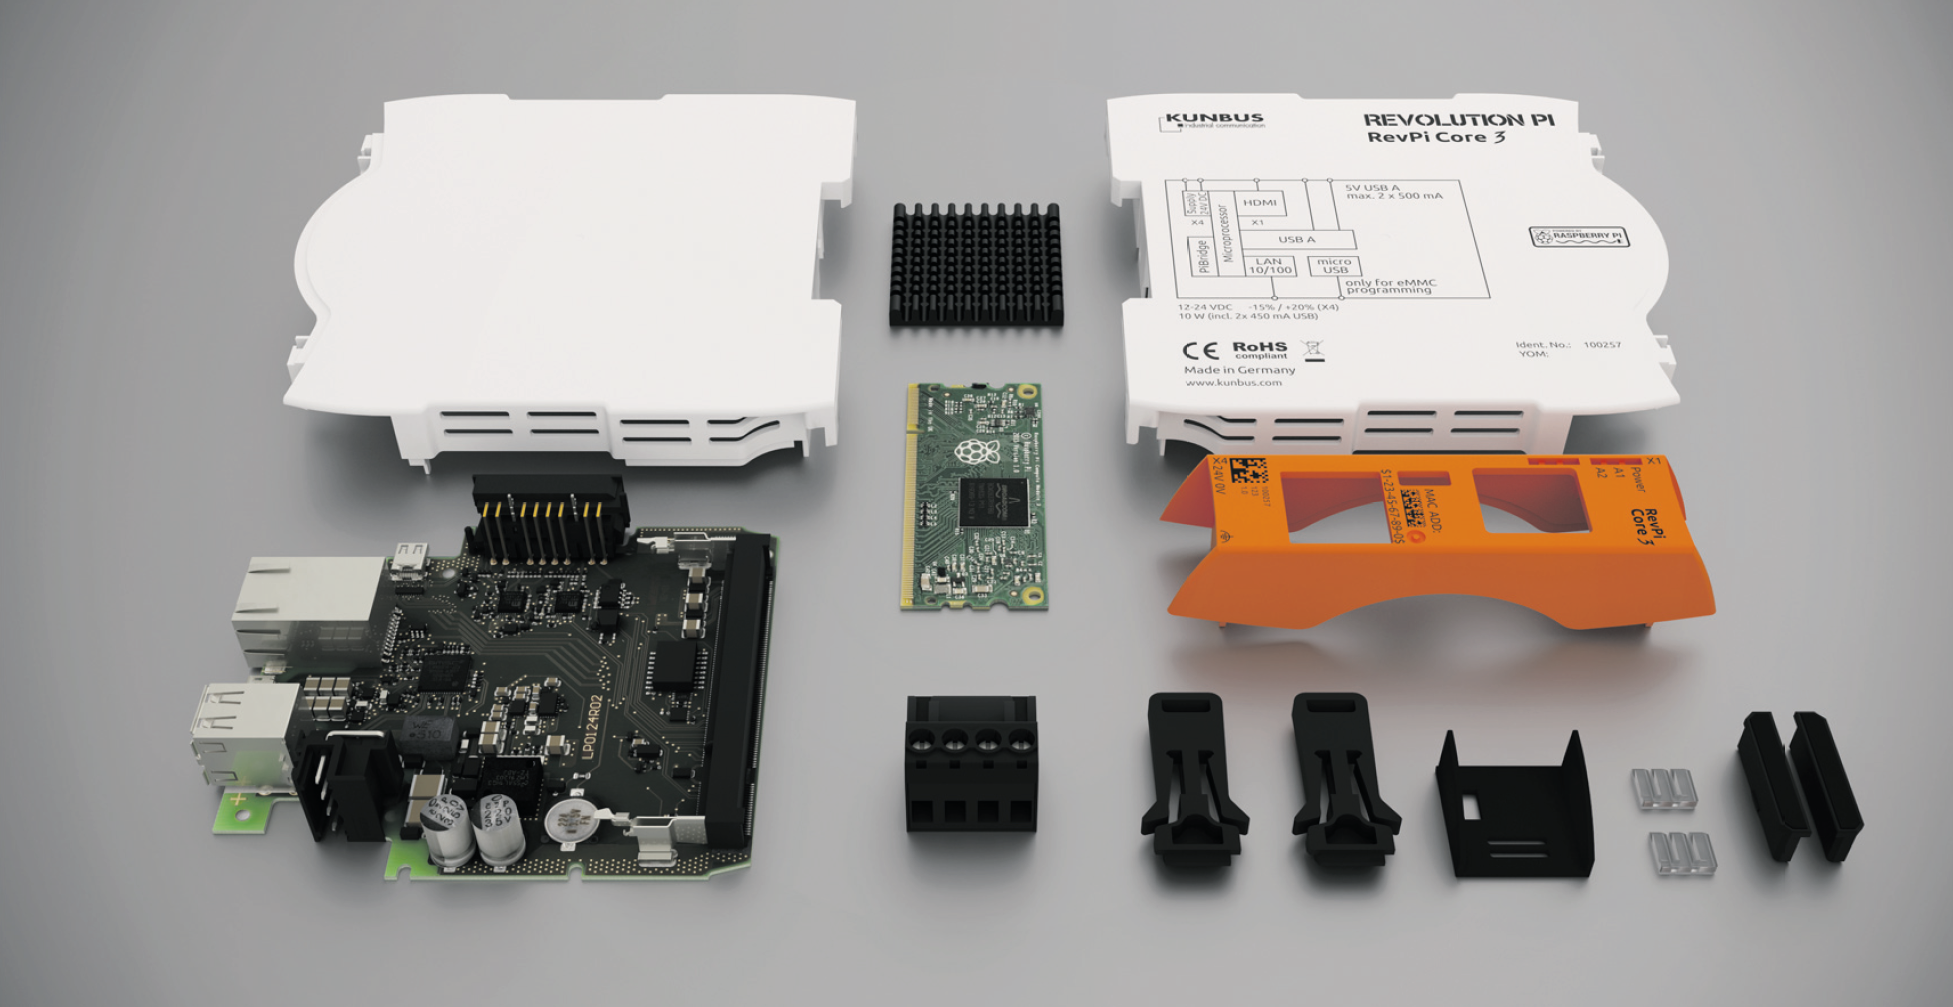
\includegraphics[width=0.85\textwidth]{doc/tex/images/revpi_teardown.png}
    \caption{Der RevPi Core 3 und seine Einzelkomponenten (Quelle: Kunbus)
      \label{fig:revpi-expl}}
\end{figure}

Spezifikationen des RevPi Core 3 \citep[Auswahl, vgl.][S. 1]{datasheet-revpi}:
\begin{itemize}
  \item{Prozessor: BCM2837}
  \item{Taktfrequenz 1,2 GHz}
  \item{Anzahl Prozessorkerne: 4}
  \item{Arbeitsspeicher: 1 GByte}
  \item{eMMC Flash Speicher: 4 GByte}
  \item{Betriebssystem: Angepasstes Raspbian mit RT-Patch}
  \item{RTC mit 24h Pufferung über wartungsfreien Kondensator}
  \item{Treiber / API: Kernel-Treiber schreibt zyklisch Prozessdaten in ein Prozessabbild, Zugriff auf Prozessabbild mittels ioctl-Anfragen oder über Linux-Dateisystem als API zu Fremdsoftware}
  \item{Kommunikationsanschlüsse: 2 x USB 2.0 A, 1 x Micro-USB, HDMI, Ethernet 10/100 Mbit/s}
  \item{Stromversorgung: min. 10,7 V, max. 28,8 V, maximal 10 Watt}
\end{itemize}

Kunbus stellt für den Revolution Pi ein auf Raspbian\footnote{Raspbian ist eine speziell 
für den Raspberry Pi angepasste Variante von Debian.} Stretch basierendes Betriebssystem bereit.
Verwendet wird der Kernel 4.9.76-rt60-v7+ in Verbindung mit dem SMP PREEMPT RT Patch.

\begin{figure}
    \centering
    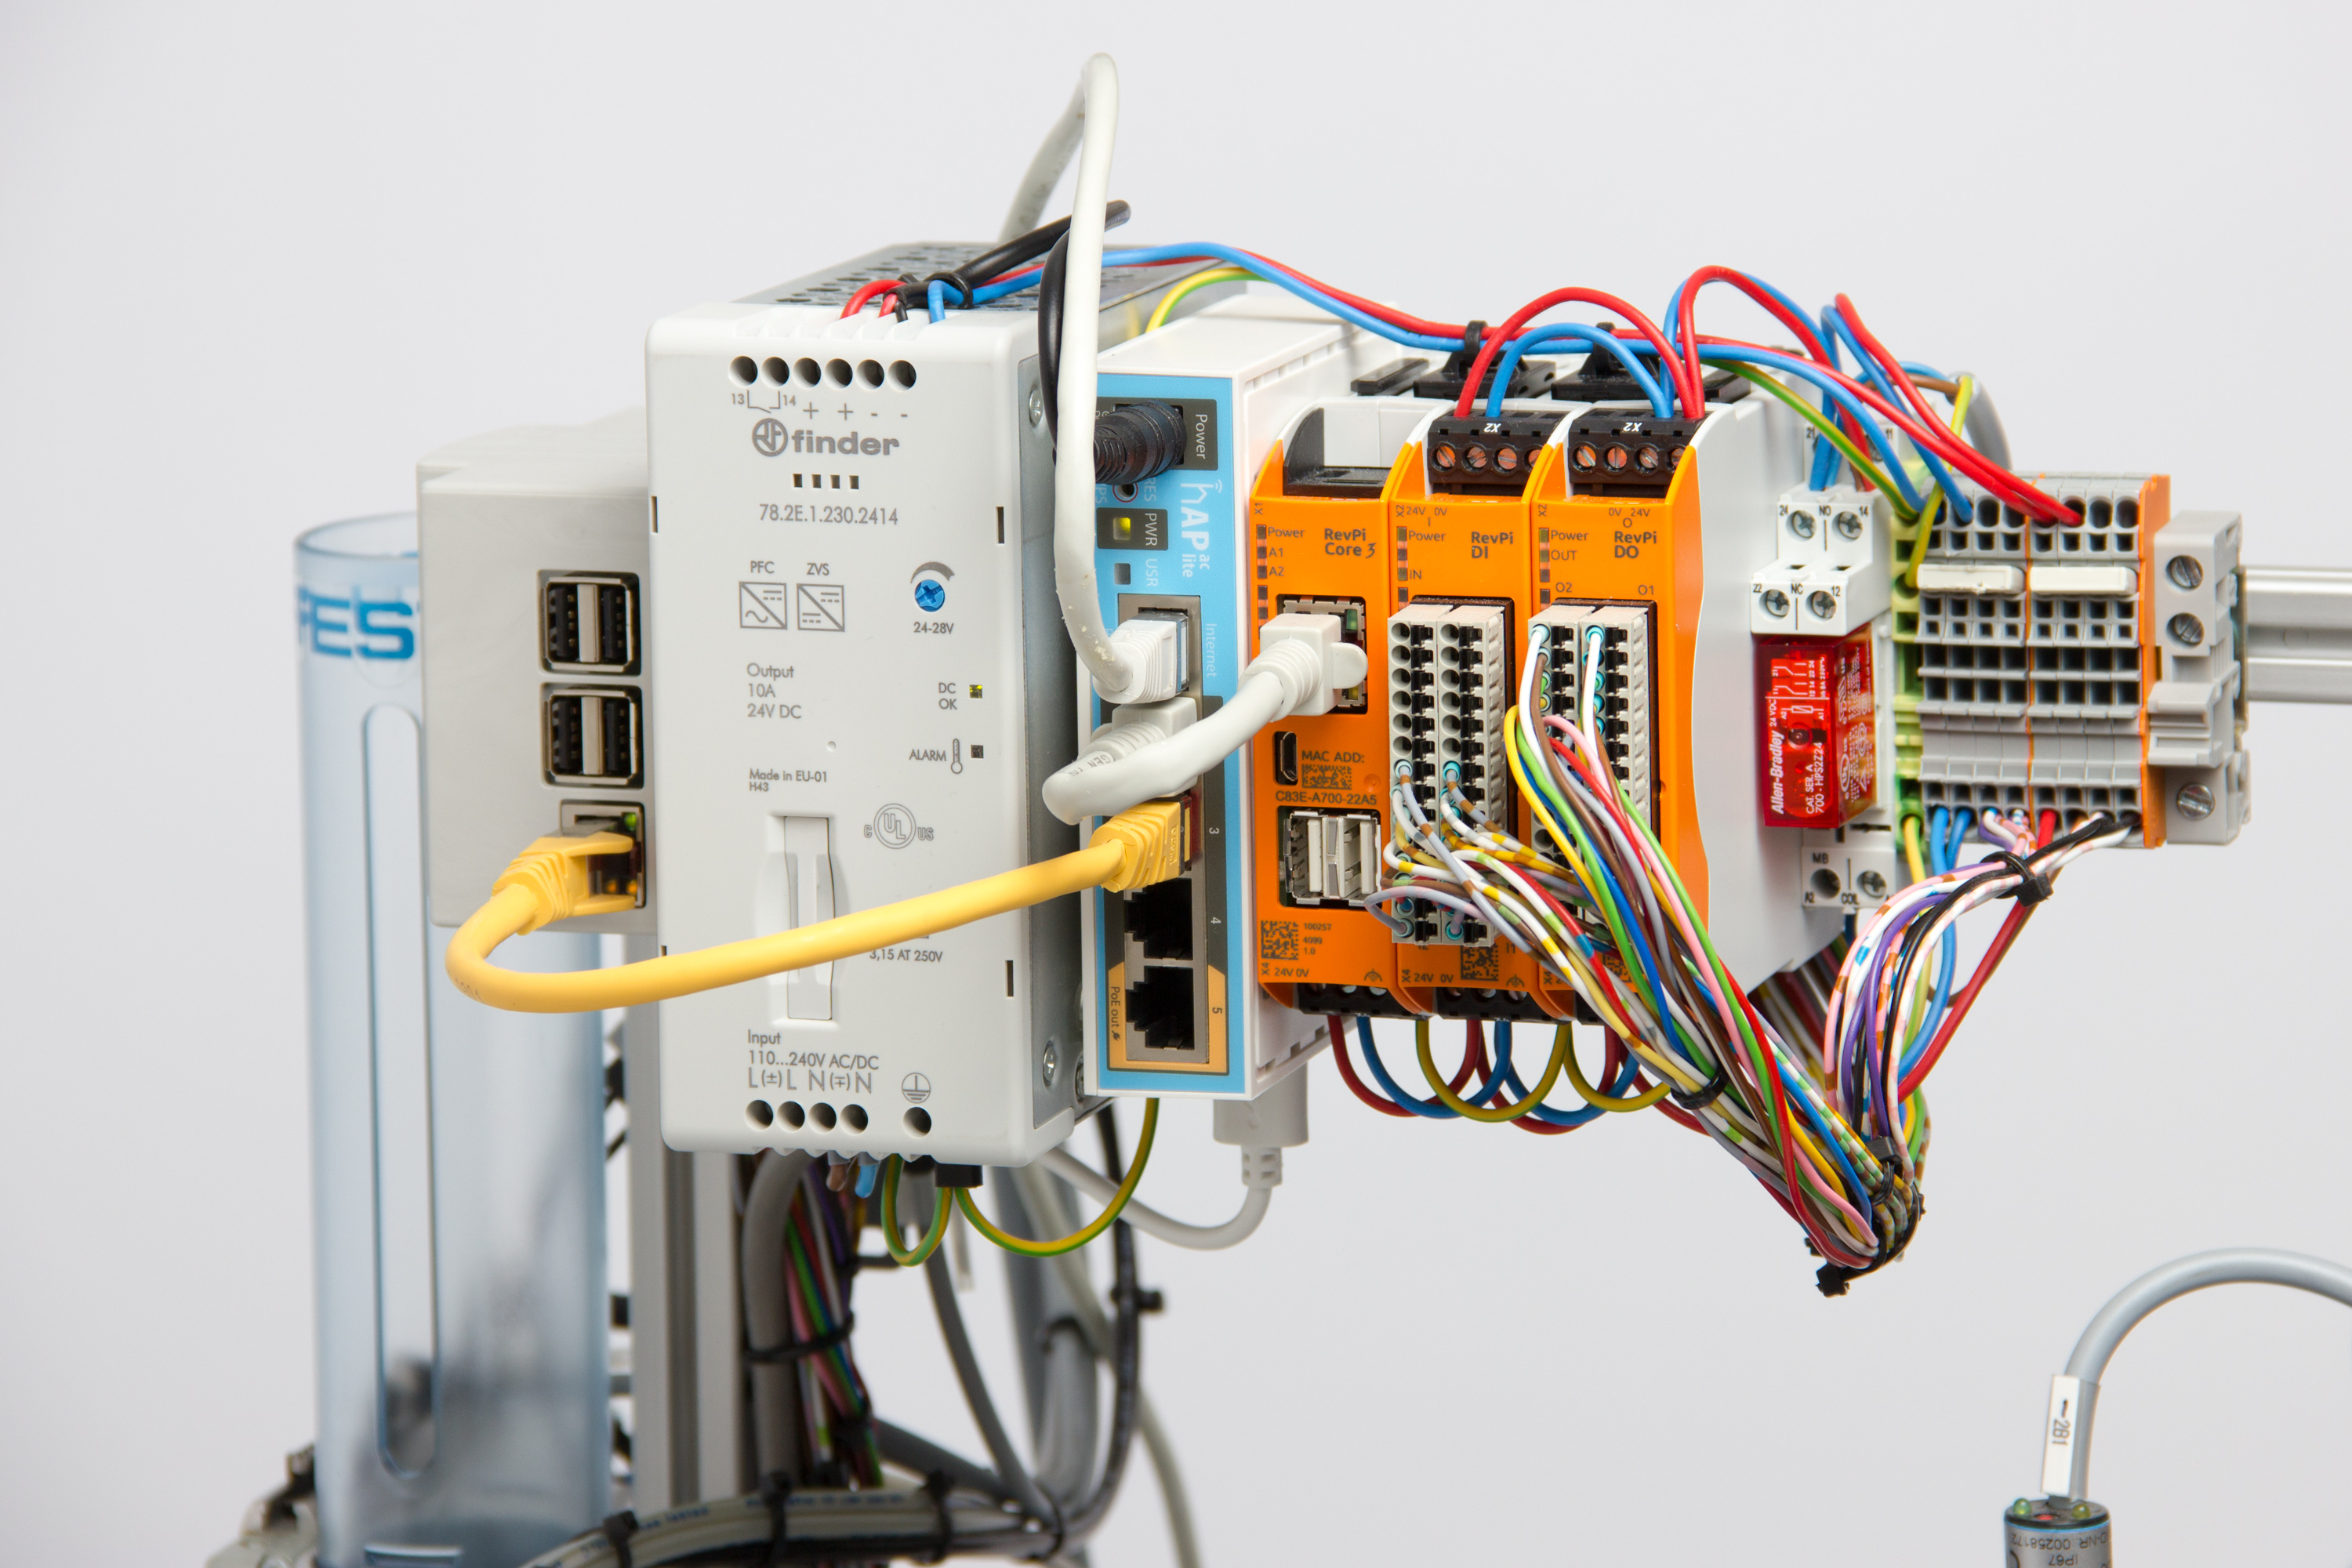
\includegraphics[trim={13cm 5cm 1cm 3cm}, clip, width=0.85\textwidth]{../photos/serverless_plc_img_8}
    \caption{Der Revolution Pi 3 mit digitalen IO-Modulen}
    \label{fig:rev-pi-io}
\end{figure}

Kunbus bietet neben dem sog. Core auch IO- und Gateway-Modulen zur Erweiterung der SPS an, siehe Bild~\ref{fig:rev-pi-io}.
Gateways dienen der Kommunikation mit externen Systemen oder Komponenten
über in der Automatisierungstechnik gängige Protokolle wie PROFIBUS oder EtherCAT. 
IO-Module erlauben die Überwachung und Steuerung von digitalen oder analogen Ein- und Ausgängen (IOs).

Kunbus deklariert die Hardware des Revolution Pi als Open-Source \citep[vgl.][S. 4]{flyer-revpi}. 
Die Schaltpläne des Revolution Pi, genauer die des RevPi Core 3 und der IO-Module, stehen auf der
Website\footnote{\label{downloads}\url{https://revolution.kunbus.com/tutorials/downloads/}} des Herstellers zum 
Download bereit. Eine Lizenz wird nicht angegeben.
Die Raspberry Pi Foundation stellt die Schaltpläne des Compute Modules des weiteren in ihrem Gitub-Repository 
zum Download bereit.

Sowohl die Raspberry Pi Foundation als auch die Kunbus GmbH pflegen aktiv ihre öffentlichen Repositories\footnote{\url{https://github.com/raspberrypi/} resp.~\url{https://github.com/RevolutionPi/}}
auf Github. 

% Kunbus konnte so einige Verbesserungen zum Linux Kernel 4.15 beitragen
% \footnote{siehe \url{https://revolution.kunbus.com/our-contribution-to-linux-4-15/}}.
% \todo{letzten Absatz evtl. weglassen? an sich nicht schlecht, passt aber irgendwie 
% nicht richtig zum Rest und stört den Lesefluss}

\subsubsection{Zugriff auf IO-Module%
        \label{sec:2-io}}
Der Zugriff auf die Ein- und Ausgänge der IO-Module erfolgt über einen RS485-Bus und einen in Form eines Kernel-Moduls bereitgestellten Treiber, genannt piControl. Der RS485-Bus ist über die serielle Schnittstelle des Compute Modules angebunden. 
piControl stellt ein Prozessabbild bereit, welches den physikalischen Zustand der Ein- und Ausgänge der IO-Module repräsentiert.
Das Prozessabbild wird, wie in der Automatisierungstechnik üblich, zyklisch aktualisiert. 
Die angestrebte Zykluszeit beträgt 5ms, kann jedoch je nach Anzahl der angeschlossenen Module auch größer sein. 
Kunbus garantiert bei drei IO-Modulen und zwei Gateway-Modulen eine Zykluszeit von 10 ms \citep[vgl.][]{web-revpi-dio}.
Die garantierte Zykluszeit ermöglicht die Umsetzung von Anwendungen mit harten Echtzeit-Anforderungen.

Fremdanwendungen können über eine Applikationsschnittstelle (API) auf das Prozessabbild zugreifen. 
Hierzu stellt das Kernel-Modul piControl sowohl \lstinline{seek}, \lstinline{read} und \lstinline{write} Methoden zur verfügung, wie auch die Möglichkeit mittels \lstinline{ioctl}-Anfragen gezielt auf einzelne Variablen des Prozessabbildes zuzugreifen.
In der englischsprachigen Wikipedia werden ioctl-Aufrufe wie folgt beschrieben:

\glqq{}The kernel is designed to be extensible, and may accept an extra module called a device driver which runs in kernel space and can directly address the device. An ioctl interface is a single system call by which userspace may communicate with device drivers. [...] The basic kernel can thus allow the userspace to access a device driver without knowing anything about the facilities supported by the device, and without needing an unmanageably large collection of system calls.

[...] ioctl calls provide a convenient way to bridge userspace code to kernel extensions. Kernel extensions can provide a location in the filesystem that can be opened by name, through which an arbitrary number of ioctl calls can be dispatched, allowing the extension to be programmed without adding system calls to the operating system.\grqq{}\citep[vgl.][]{web-wiki-ioctl}

Der Quellcode von piControl steht unter der GNU General Public License Version 2 (GNU GPLv2) und ist 
auf Github verfügbar\footnote{\url{https://github.com/RevolutionPi/piControl}}. Als Einstieg in die 
Entwicklung eigener Steuerungsprogramme liefert Kunbus das C-Programm piTest mit. Dieses verwendet 
piControl und erlaubt dem Nutzer über Kommandozeilen-Parameter die angeschlossenen IO-Module zu steuern.

\begin{figure}[h]
    \centering
    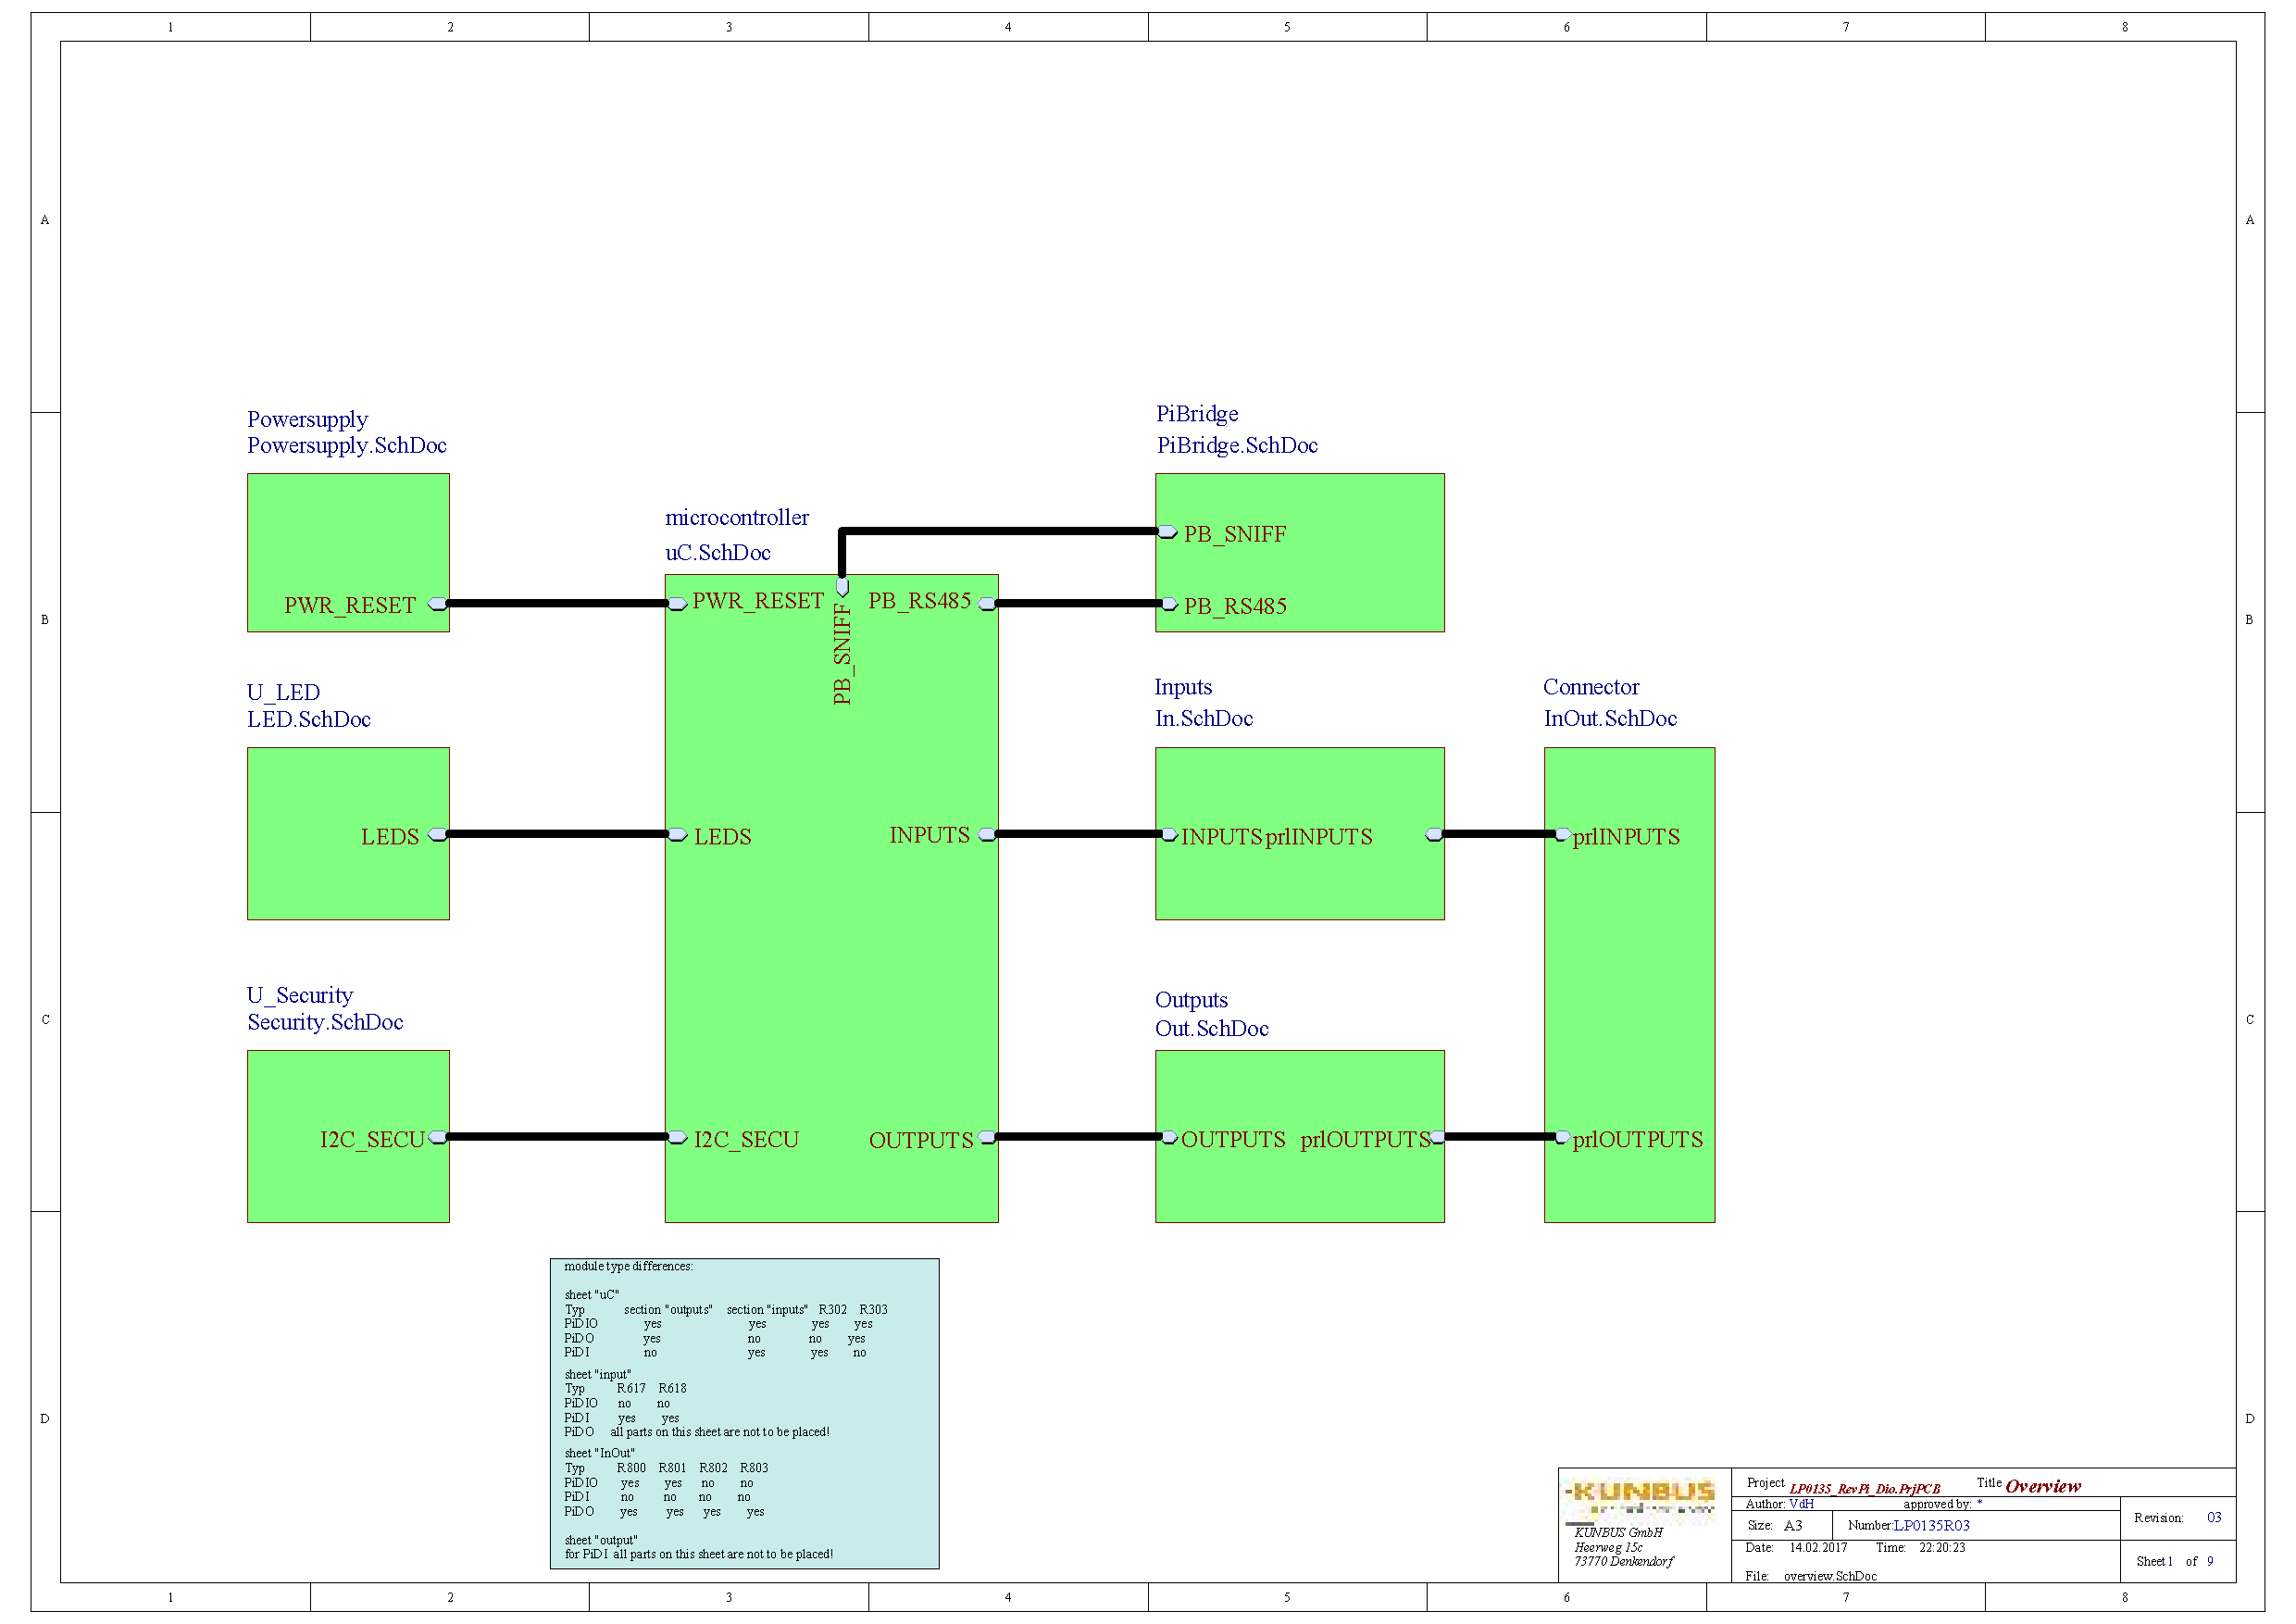
\includegraphics[trim={4cm 7cm 10.5cm 7.3cm}, clip, width=\textwidth]{literature/SchematicPrintsRevPi-DIO}
    \caption{Schematische Darstellung eines DIO-Moduls (Quelle: Kunbus\textsuperscript{\ref{downloads}})
      \label{fig:dio}}
\end{figure}

Jedes der IO-Module stellt ein eigenständiges eingebettetes System dar. Es verfügt
über einen Microcontroller, welcher die IOs bereitstellt und über einen RS485-Bus
mit dem Revolution Pi kommuniziert (siehe Bild~\ref{fig:dio}). 
Kunbus stellt exemplarisch den Quellcode eines DIO-Moduls unter der MIT Lizenz zur
Verfügung\footnote{\url{https://github.com/RevolutionPi/IODeviceExample}}. 


\subsection{Echtzeit und Multitasking unter Linux -- preemptRT und posix%
     \label{sec:2-echtzeit}}
     
Moderne Betriebssysteme realisieren Multitasking i.d.R.\,in Form des präemptiven Multitasking. 
Der Kernel verfügt über einen sog. Scheduler. Dieser priorisiert alle Prozesse und weist ihnen 
Rechenzeit in sog. Time Slots zu. Die Größe der Zeitfenster sowie die Ausführungsreihenfolge 
ist von der Priorität eines Prozesses abhängig. Besonders an einem präemptiven im Gegensatz zu einem kooperativen Scheduler ist dessen Fähigkeit, Tasks während ihrer Ausführung zu unterbrechen bzw. zu pausieren, wenn diese eine bestimmte Dauer überschreiten oder ein höher priorisierter Prozess (bspw. ausgelöst durch einen Interrupt oder durch eine inhärente Periodizität) Rechenleistung benötigt.

Eine Sonderform des präemptiven Multitasking ist das präemptible Multitasking. Hierbei werden auch Teile 
des Kernels als Threads durch den Scheduler ausgeführt. Dieser ist somit in der Lage, auch Prozesse des Kernels
zu unterbrechen, wenn andere Anwendungen Prozessorzeit oder Zugriff auf andere Systemressourcen benötigen
\citep[vgl.][]{web-wiki-praempt}.
     
Der Linux-Kernel implementiert unterschiedliche Präemptions-Modelle \citep[vgl.][/preemption\_models]{web-linuxwiki-basics}:

\begin{itemize}
  \item No Forced Preemption (server):
  Ausgelegt auf maximal möglichen Durchsatz, lediglich Interrupts und
  System-Call-Returns bewirken Präemption.

  \item Voluntary Kernel Preemption (Desktop):
  Neben den implizit bevorrechtigten Interrupts und System-Call-Returns gibt es
  in diesem Modell weitere Abschnitte des Kernels in welchen Preämption explizit
  gestattet ist.

  \item Preemptible Kernel (Low-Latency Desktop):
  In diesem Modell ist der gesamte Kernel, mit Ausnahme sog.~kritischer Abschnitte
  präemptible. Nach jedem kritischen Abschnitt gibt es einen impliziten Präemptions-Punkt.

  \item Preemptible Kernel (Basic RT):
  Dieses Modell ist dem zuvor genannten sehr ähnlich, hier sind jedoch alle Interrupt-Handler
  als eigenständige Threads ausgeführt.

  \item Fully Preemptible Kernel (RT):
  Wie auch bei den beiden zuvor genannten Modellen ist hier der gesamte Kernel
  präemtible. Die Anzahl und Dauer der nicht-präemtiblen kritischen Abschnitte
  ist auf ein notwendiges Minimum beschränkt. Alle Interrupt-Handler sind als
  eigenständige Threads ausgeführt, Spinlocks durch Sleeping-Spinlocks und Mutexe
  durch sog.~RT-Mutexe ersetzt.

\end{itemize}

Lediglich ein präemtibler Kernel kann hartes Echtzeit-Verhalten realisieren, 
da nur hier eine maximale Antwortzeit garantiert werden kann.
Viele Prozesse in der Automatisierungstechnik erfordern harte Echtzeit. 
Eine verspätete Antwort auf eine Anfrage, 
wie etwa das Signal eines Lagenendschalters oder eines Notausschalters kann hier nicht nur über
den Erfolg eines Prozesses, sondern auch über das Leben der daran beteiligten Mitarbeiter entscheiden.
Für weiterführende Erklärungen bzgl.\,Echtzeit, Mutexen und 
Spinlocks sei an dieser Stelle auf die Vorlesung verwiesen~\citep{script-peter}.


\subsubsection{preemptRT%
        \label{sec:2-preemptRT}}

Der Kernel des auf dem Revolution Pi installierten Raspbian mit PREEMP\_RT Patch fällt 
in die Kategorie des \glqq{}Fully Preemptible Kernels\grqq{} (siehe Abschnitt \ref{sec:2-echtzeit}).
Das zugrunde liegende Prinzip lässt sich wie folgt formulieren: Nur Code, welcher absolut nicht-präemtible sein darf, ist es
gestattet nicht-präemtible zu sein. Ziel ist folglich, die Menge des nicht-präemtiblen 
Codes im Linux-Kernel auf das absolut notwendige Minimum zu reduzieren.

Dies wird durch Verwendung folgender Mechanismen erreicht~\citep[vgl.][]{web-linuxwiki-details}:

\begin{itemize}
  \item Hochauflösende Timer
  \item Sleeping Spinlocks
  \item Threaded Interrupt Handlers
  \item rt\_mutex
  \item RCU
\end{itemize}

Diese Mechanismen sind bspw. im Linux-Wiki\footnote{siehe \url{https://wiki.linuxfoundation.org/realtime/documentation/technical_details}} ausführlich beschrieben.

\subsubsection{POSIX%
        \label{sec:2-posix}}
Das Portable Operating System Interface (POSIX) bezeichnet eine Sammlung von Standards, 
welche auf dem Unix-System basieren, jedoch nicht auf dieses beschränkt sind.

Der Wechsel zwischen verschiedenen Unix-Distributionen brachte oft Kompatibilitätsprobleme mit sich. 
Dieser Mangel an Portabilität erschwerte Benutzern und Entwicklern die Verwendung bzw. Bereitstellung 
von Software auf unterschiedlichen Systemen. 
Das Institut für Elektrotechnik und Elektronik (IEEE) begann 1984 mit der Entwicklung des Unix-Standards.
Sie entwickelten das, was heute als Single UNIX Specification bekannt ist und allgemein als POSIX bezeichnet wird~\citep[vgl.][]{web-debianwiki-posix}.
Das Konsortium \glqq{}The Open Group\grqq{} überwacht die weitere Entwicklung dieses Standards.
Ferner stellt es einen Teil der POSIX-Spezifikation frei zur Verfügung~\citep[vgl.][]{web-opengroup-posix}.

Die aktuelle Version POSIX.1-2017 ist verfügbar als IEEE Standard 1003.1-2017 sowie in Form der \glqq{}The Open Group Technical Standard Base Specifications\grqq{}, Ausgabe 7. POSIX.1-2017 definiert eine Standard-Betriebssystemschnittstelle und -umgebung, einschließlich eines Befehlsinterpreters (auch Shell genannt) und gängiger Dienstprogramme zur Unterstützung der Portabilität von Anwendungen auf Quellcode-Ebene. POSIX.1-2017 ist sowohl für Anwendungsentwickler als auch für Systemimplementierer gedacht und umfasst vier Hauptkomponenten \citep[vgl.][]{web-opengroup-overview}:
\begin{itemize}
    \item Basisdefinitionen:\\
          Allgemeine Begriffe, Konzepte und Schnittstellen einschließlich Hilfskonventionen und C-Headern
          
    \item Systemschnittstellen:\\
          Definitionen für Systemdienstfunktionen und Unterprogramme, C-spezifische Systemdienste, Portabilität
        
    \item Shell und Dienstprogramme:\\
          Definitionen für eine Schnittstelle zur Befehlsinterpretation von Diensten und gängige Hilfsprogramme
    
    \item Begründungen und Historie
\end{itemize}

Debian basiert auf Linux und verwendet den Linux-Kernel. Linux ist zu großen Teilen POSIX-kompatibel. Debian ist jedoch nicht POSIX-zertifiziert, da diese Zertifizierung mit hohen Kosten verbunden ist\citep[vgl.][Kapitel 4.4.]{web-debian-faq}.

Beide Kernkomponenten des in dieser Arbeit vorgestellten Projektes nutzen Komponenten von Linux, 
welche an den POSIX-Standard angelehnt sind: open62541 verwendet u.a.\,POSIX-Threads und
Mutexe~\citep[vgl.][pthread.h]{web-opengroup-pthread}, piControl nutzt POSIX-Semaphoren
\citep[vgl.][semaphore.h]{web-opengroup-semaphore}. 


\subsection{OPC-UA und open62541%
     \label{sec:2-opc}}
In diesem Abschnitt sollen Möglichkeiten des Datenaustausch zwischen Komponenten der
Automatisierungstechnik vorgestellt werden. OPC-UA stellt einen offenen, IP-basierten Kommunikationsstandard
für Sensoren und Steuerungen dar. open62541 ist eine freie Client- sowie Server-Implementierung dieses
Standards, geschrieben in C.


\subsubsection{OPC UA%
        \label{sec:2-opcua}}

Open Platform Communications (OPC) ist eine Familie von Standards zur herstellerunabhängigen
Kommunikation von Maschinen (M2M) in der Automatisierungstechnik. Die sog. OPC Task Force, zu deren
Mitgliedern verschiedene etablierte Firmen der Automatisierungsindustrie gehören, veröffentlichte
die OPC Specification Version 1.0 im August 1996.
Motiviert ist dieser offene Standard durch die Erkenntniss, dass die Anpassung der
zahlreichen Herstellerstandards an individuelle Infrastrukturen und Anlagen einen
großen Mehraufwand verursachen.
Die Wikipedia beschreibt das Anwendungsgebiet für OPC wie folgt \citep[vgl.][]{web-wiki-opc}:

\glqq{}OPC wird dort eingesetzt, wo Sensoren, Regler und Steuerungen verschiedener Hersteller
ein gemeinsames Netzwerk bilden. Ohne OPC benötigten zwei Geräte zum Datenaustausch
genaue Kenntnis über die Kommunikationsmöglichkeiten des Gegenübers. Erweiterungen
und Austausch gestalten sich entsprechend schwierig. Mit OPC genügt es, für jedes
Gerät genau einmal einen OPC-konformen Treiber zu schreiben. Idealerweise wird
dieser bereits vom Hersteller zur Verfügung gestellt. Ein OPC-Treiber lässt sich
ohne großen Anpassungsaufwand in beliebig große Steuer- und Überwachungssysteme
integrieren.

OPC unterteilt sich in verschiedene Unterstandards, die für den jeweiligen Anwendungsfall
unabhängig voneinander implementiert werden können. OPC lässt sich damit verwenden
für Echtzeitdaten (Überwachung), Datenarchivierung, Alarm-Meldungen und neuerdings
auch direkt zur Steuerung (Befehlsübermittlung).\grqq{}

OPC basiert in der ursprünglichen Spezifikation (auch als OPC DA bezeichnet) auf Microsofts DCOM-Spezifikation.
DCOM macht Funktionen und Objekte einer Anwendung anderen Anwendungen im Netzwerk
zugänglich. Der OPC-Standard definiert entsprechende DCOM-Objekte um mit anderen
OPC-Anwendungen Daten austauschen zu können. Die Verwendung von DCOM bindet Anwender
jedoch an Betriebssysteme von Microsoft. 

\begin{figure}
    \centering
    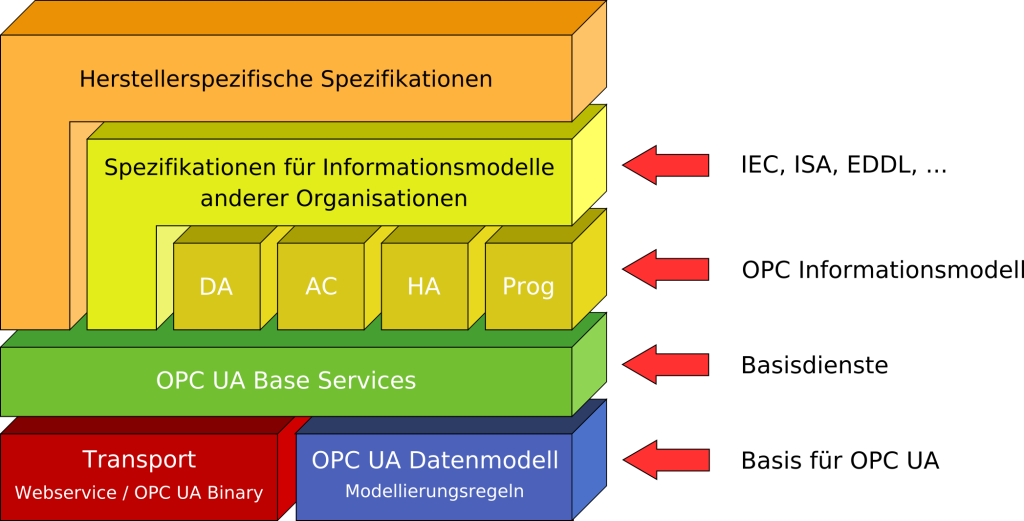
\includegraphics[width=0.85\textwidth]{images/UA_Architecture_1024.png}
    \caption{Die OPC Unified Architecture. Grafik von Gerhard Gappmeier - ascolab GmbH, CC BY-SA 3.0}
    \label{fig:opc-unified-architecture}
\end{figure}
% Evtl Grafik: Von Gerhard Gappmeier - ascolab GmbH, CC BY-SA 3.0, https://de.wikipedia.org/w/index.php?curid=1892069

Die ursprüngliche OPC Spezifikation wurde 2006 durch die Entwicklung der 
OPC Unified Architecture (OPC UA) überholt. 
Diese zeichnet sich durch eine Service-orientierte Architektur (SOA) aus, deren Struktur
aus mehreren Schichten besteht, siehe Abbilung~\ref{fig:opc-unified-architecture}. 
Über der untersten Schicht, dem Betriebssystem des Servers, verbindet eine Portabilitäts-Schicht 
den sog.\, UA ANSI C Stack mit einer API. Diese API kann bspw.\,in C++ geschrieben sein, 
und erlaubt die Anbindung der obersten Schicht, der Anwendungsschicht~\citep[vgl.][]{web-spec-opc}.
OPC UA setzt auf einem eigenen Kommunikationsstack auf; die Verwendung von DCOM
und damit die Bindung an Microsoft wurden aufgelöst.

Neben Architektur und Kommunikationsschnittstellen wird in der OPC Spezifikation auch ein 
Informationsmodell definiert. Die deutschsprachige Wikipedia beschreibt dieses wie folgt: 

\glqq{}Das OPC[-UA]-Informationsmodell ist nicht mehr nur eine Hierarchie aus Ordnern, Items
und Properties. Es ist ein sogenanntes Full-Mesh-Network aus Nodes, mit dem neben
den Nutzdaten eines Nodes auch Meta- und Diagnoseinformationen repräsentiert werden. [...]
Ein Node ähnelt einem Objekt aus der objektorientierten Programmierung. Ein Node
kann Attribute besitzen, die gelesen werden können. Es ist möglich Methoden zu definieren und aufzurufen. [...]
Weiterhin werden Events unterstützt, die versendet werden können
(AE (Alarms \& Events), DA DataChange), um bestimmte Informationen zwischen Geräten
auszutauschen. Ein Event besitzt unter anderem einen Empfangszeitpunkt, eine Nachricht
und einen Schweregrad. Die o.\,g. Nodes werden sowohl für die Nutzdaten als auch
alle anderen Arten von Metadaten verwendet. Der damit modellierte OPC-Adressraum
beinhaltet nun auch ein Typmodell, mit dem sämtliche Datentypen spezifiziert werden.\grqq{}


\subsubsection{open62541%
        \label{sec:2-open62541}}
open62541 ist eine offene und freie Implementierung von OPC UA. 
Die in C geschriebene Bibliothek stellt eine beständig zunehmende Anzahl der im OPC UA Standard definierten
Funktionen bereit. Sie kann sowohl zur Erstellung von OPC-Servern als auch von -Clients
genutzt werden. Ergänzend zu der unter der Mozilla Public License v2.0 lizensierten
Bibliothek stellt das open62541 Projekt auch Beispielprogramme unter einer CC0 Lizenz
zur Verfügung.
Zu den Unterstützern des Projektes zählen u.a.\, die RWTH Aachen, das Frauenhofer IOSB sowie die TU Dresden.

Die Bibliothek eignet sich auch für die Entwicklung auf eingebetteten Systemen und
Microcontrollern. Die Größe einer Server-Binary kann weniger als 100kB betragen.

Folgende Auswahl an Eigenschaften und Funktionen zeichnet die in dieser Arbeit verwendete
Version 0.3 von open62541 aus:
\begin{itemize}
  \item Kommunikationionsstack
  \begin{itemize}
      \item OPC UA Binär-Protokoll (HTTP oder SOAP werden gegenwärtig nicht unterstützt)
      \item Austauschbare Netzwerk-Schicht, welche die Verwendung eigener Netzwerk-APIs
      erlaubt.
      \item Verschlüsselte Kommunikationion
      \item Asynchrone Dienst-Anfragen im Client
  \end{itemize}
  \item Informationsmodell
  \begin{itemize}
    \item Unterstützung aller OPC UA Node-Typen, inkl.~Methoden
    \item Hinzufügen und Entfernen von Nodes und Referenzen zur Laufzeit.
    \item Vererbung und Instanziierung von Objekt- und Variablentypen
    \item Zugriffskontrolle auch für einzelne Nodes
  \end{itemize}
  \item Subscriptions
  \begin{itemize}
    \item Erlaubt die Überwachung (subscriptions / monitoreditems)
    \item Sehr geringer Ressourcenbedarf pro überwachtem Wert
  \end{itemize}
  \item Code-Generierung auf XML-Basis
  \begin{itemize}
    \item Erlaubt die Erstellung von Datentypen
    \item Erlaubt die Generierung des serverseitigen Informationsmodells
  \end{itemize}
\end{itemize}

Weiterführende Informationen und Code-Beispiele bietet die ausführliche Dokumentation des Projektes~\citep[siehe]{web-open62541} sowie der kommentierte Quelltext.

% % % Imports nur für Referenzenauflösung während des Schreibens! Vorm Kompilieren auskommentieren!
% \bibliography{0_hauptdatei}
% \input{1_einleitung}
% \input{2_grundlagen}
% \input{3_konzeption}
% \input{4_implementierung}
% \input{5_tests}
% \input{6_zusammenfassung}
% \input{anhang}
% % Ende Imports

\section{Systemkonzept%
  \label{sec:3-konzeption}}
Auf Basis der in Abschnitt [...] vorgestellten Möglichkeiten folgt nun die Ausarbeitung eines Konzepts.

\subsection{Anbindung der IO an den OPC-Server%
     \label{sec:3-anbindung}}

\subsection{Integration des OPC-Servers in das System%
     \label{sec:3-integration}}

% % % Imports nur für Referenzenauflösung während des Schreibens! Vorm Kompilieren auskommentieren!
% \bibliography{0_hauptdatei}
% \input{1_einleitung}
% \input{2_grundlagen}
% \input{3_konzeption}
% \input{4_implementierung}
% \input{5_tests}
% \input{6_zusammenfassung}
% \input{anhang}
% % Ende Imports

\section{Implementierung%
  \label{sec:4-implementierung}}
Das folgende Kapitel stellt in Auszügen die Implementierung des OPC-Servers sowie die Anbindung an die IO-Module
der SPS dar. Der Schwerpunkt liegt hierbei auf der Funktionsweise des piControl-Treibers und dessen Integration in das Projekt. Abschnitt~\ref{sec:4-picontrol} erklärt die zum Schreibens eines Bits verwendeten Funktionsaufrufe.
Zuvor soll jedoch in Abschnitt~\ref{sec:4-open62541} der Teil des OPC-Servers vorgestellt werden, welcher auf besagten Treiber zugreift. 

\subsection{Implementierung des OPC-Servers%
     \label{sec:4-open62541}}
Wie im vorangegangenen Abschnitt~\ref{sec:3-integration} begründet, soll die Verknüpfung zwischen dem Prozessabbild der SPS und den auf dem OPC-Server bereitgestellten Werten über sog.\,Datenquellen erfolgen. Hierzu ist zunächst eine Callback-Methode zu implementieren, welche bei einem Lese- oder Schreibzugriff auf eine Variable aufgerufen wird. Die Verknüpfung zwischen Callback-Methode und Variable muss manuell erfolgen.

\begin{lstlisting}[language={c},firstnumber=237,caption={Auszug der Methode \lstinline{linkDataSourceVariable} in \lstinline{variables.c}\label{lst:4-linkDataSourceVariable}}]
extern UA_StatusCode
 linkDataSourceVariable(UA_Server *server, UA_NodeId nodeId) {
     bool readonly = false;
     UA_DataSource dataSourceVariable;
     UA_StatusCode rc; |>\setcounter{lstnumber}{254}<|

     dataSourceVariable.read = readDataSourceVariable;
     if (!readonly)
        dataSourceVariable.write = writeDataSourceVariable;
     else
        dataSourceVariable.write = writeReadonlyDataSourceVariable;

     return UA_Server_setVariableNode_dataSource(server, nodeId, dataSourceVariable);
 }
\end{lstlisting}

\begin{figure}[h]
    \centering
    \includegraphics[width=0.42\textwidth]{doc/img/OPC_RevPiDO.pdf}
    \caption{Auszug des verwendeten Nodesets, hier Digitalausgang 1 des Versuchsaufbaus
      \label{fig:opc-do}}
\end{figure}

Die in Listing~\ref{lst:4-linkDataSourceVariable} abgebildete Methode \lstinline{linkDataSourceVariable()} erzeugt ein Struct vom Typ \lstinline{UA_DataSource}. In diesem werden dem Lesen und Schreiben einer OPC-Variablen entsprechende Callback-Methoden zugewiesen. Die Verknüpfung einer OPC-Variable, genauer ihrer NodeId, mit der zuvor definierten Datenquelle erfolgt über die von open62541 bereitgestellte Methode \lstinline{UA_Server_setVariableNode_dataSource()}. Vor dem Lesen und nach dem Schreiben dieser Variable werden von nun an die entsprechenden Callbacks aufgerufen.
     
\begin{lstlisting}[language={c},firstnumber=168,caption={Auszug des Callbacks \lstinline{writeDataSourceVariable} in \lstinline{variables.c}\label{lst:4-writeDataSourceVariable}}]  
extern UA_StatusCode
 writeDataSourceVariable(UA_Server *server,
            const UA_NodeId *sessionId, void *sessionContext,
            const UA_NodeId *nodeId, void *nodeContext,
            const UA_NumericRange *range, const UA_DataValue *dataValue) {

    UA_StatusCode retval  = UA_STATUSCODE_GOOD;
    UA_NodeId *nameNodeId = UA_malloc(sizeof(UA_NodeId));
    UA_QualifiedName nameQN = UA_QUALIFIEDNAME(1, "Name");
    UA_Variant nameVar;
    UA_Boolean bit;

    retval |= findSiblingByBrowsename(server, nodeId, &nameQN, nameNodeId);
    retval |= UA_Server_readValue(server, *nameNodeId, &nameVar);
    retval |= UA_Boolean_copy(dataValue->value.data, &bit);

    |>\tikzmarkin[set border color=martinired]{writeIO}<|PI_writeSingleIO(String_fromUA_String(nameVar.data), &bit, false);                                                 |>\tikzmarkend{writeIO}<|

    free(nameNodeId);
    return retval;
 }
\end{lstlisting}

Listing~\ref{lst:4-writeDataSourceVariable} zeigt die Callback-Methode, welche nach dem Schreiben einer Variablen auf dem OPC-Server aufgerufen wird.
Dieser Methode wird neben der NodeId der mit ihr verknüpften Variablen auch der Wert dieser in Form eines Zeigers auf ein Struct vom Typ \lstinline{UA_DataValue} übergeben.

Die Gestaltung des hier verwendeten Nodesets sieht vor, dass in einer OPC-Variablen \lstinline{"Name"} der Bezeichner des zu schreibenden Digitalausgangs hinterlegt ist, siehe Abbildung~\ref{fig:opc-do}. Dies erlaubt eine Rekonfiguration der Ein- und Ausgänge der SPS ohne Änderungen im Programmcode des OPC-Servers vornehmen zu müssen.
Es ist daher erforderlich, nach jedem Schreiben einer mit einem Digitalausgang verknüpften Variablen, hier \lstinline{"Value"}, dessen Bezeichner \lstinline{"Name"} abzufragen. 
Dies geschieht in den Zeilen 180 und 181.
Anschließend wird dieser Bezeichner sowie der zu schreibende Wert der Methode \lstinline{PI_writeSingleIO()} übergeben, welche wiederum die Interaktion mit piControl übernimmt (vgl. Abschnitt \ref{sec:4-picontrol}).
 
\subsection{Integration von piControl%
     \label{sec:4-picontrol}}
In Abschnitt~\ref{sec:2-io} wurde die Anbindung der IO-Module des Revolution Pi sowie die Funktionsweise von piControl aus Anwendersicht beschrieben. Die verfügbare Literatur beschränkt sich auch auf lediglich diese Sicht; eine weiterführende Dokumentation für Entwickler gibt es, neben der in Abschnitt~\ref{sec:3-anbindung} vorgestellten Manpage, nicht. 
In diesem Abschnitt soll daher der Quellcode von piControl sowie dessen Verwendung im Projekt genauer betrachtet werden.
Hierzu wird exemplarisch die in Abschnitt~\ref{sec:4-open62541} eingeführte Methode \lstinline{PI_writeSingleIO()} untersucht.
Diese Methode ermöglicht das Setzen eines einzelnen Bits im Prozessabbild der SPS, und damit das Schalten eines digitalen Ausgangs auf einem IO-Modul.
Die äquivalente Methode \lstinline{int piControlGetBitValue(SPIValue *pSpiValue)} zum Lesen eines Bits bzw. Eingangs funktioniert analog und soll daher an dieser Stelle nicht dediziert erörtert werden.

\begin{lstlisting}[language={c},firstnumber=97,
                   caption={Setzen eines phsikalischen, digitalen Ausgangs in \lstinline{revpi.c}
                   \label{lst:4-PI_writeSingleIO}}]
extern void PI_writeSingleIO(char *pszVariableName, bool *bit, bool verbose)
{
	int rc;
	SPIVariable sPiVariable;
	SPIValue sPIValue;

	strncpy(sPiVariable.strVarName, pszVariableName, sizeof(sPiVariable.strVarName));
	rc = piControlGetVariableInfo(&sPiVariable);
	if (rc < 0) {
		printf("Cannot find variable '%s'\n", pszVariableName);
		return;
	}

		sPIValue.i16uAddress = sPiVariable.i16uAddress;
		sPIValue.i8uBit = sPiVariable.i8uBit;
		sPIValue.i8uValue = *bit;
		rc = |>\tikzmarkin[set border color=martinired]{setBitValue}<|piControlSetBitValue(&sPIValue)|>\tikzmarkend{setBitValue}<|;
		if (rc < 0)
			printf("Set bit error %s\n", getWriteError(rc));
		else if (verbose)
			printf("Set bit %d on byte at offset %d. Value %d\n", sPIValue.i8uBit, sPIValue.i16uAddress,
			       sPIValue.i8uValue);
}
\end{lstlisting}

Der Programmcode in Listing~\ref{lst:4-PI_writeSingleIO} ist Teil des implementierten OPC-Servers. In diesem wird auf zwei Funktionen des piControl-Treibers zugegriffen. 
Beiden Methoden wird als Argument ein Zeiger auf ein Struct vom Typ \lstinline{SPIValue} übergeben. Der im Struct abgelegte Name wird mittels \lstinline{piControlGetVariableInfo(&sPIValue)} zu einer Adresse im Prozessabbild aufgelöst. Diese wird in \lstinline{sPIValue.i16uAdress} gespeichert. Der Wert der Variablen wird anschließend mittels \lstinline{piControlSetBitValue(&sPIValue)} an dieser Adresse in das Prozessabbild geschrieben.

\begin{lstlisting}[language={c},firstnumber=309,caption={Methode \lstinline{piControlSetBitValue} in \lstinline{piControlIf.c}\label{lst:4-piControlSetBitValue}}]
int |>\tikzmarkin[set border color=martiniblue]{setBitValueFcn}<|piControlSetBitValue(SPIValue *pSpiValue)|>\tikzmarkend{setBitValueFcn}<|
{
    piControlOpen();

    if (PiControlHandle_g < 0)
	    return -ENODEV;

    pSpiValue->i16uAddress += pSpiValue->i8uBit / 8;
    pSpiValue->i8uBit %= 8;

    if (|>\tikzmarkin[set border color=martinired]{ioctl}<|ioctl(PiControlHandle_g, KB_SET_VALUE, pSpiValue)|>\tikzmarkend{ioctl}<| < 0)
	    return errno;

    return 0;
}
\end{lstlisting}

Die in Listing~\ref{lst:4-piControlSetBitValue} dargestellte Methode \lstinline{piControlSetBitValue} ist lediglich eine Hüllfunktion (häufig auch als Wrapper-Funktion bezeichnet) für einen Aufruf des \lstinline{ioctl} Kernel-Moduls.
Folgende Parameter werden übergeben:
\lstinline{PiControlHandle_g} ist die Referenz auf die Geräte-Datei des piControl-Treibers. \lstinline{KB_SET_VALUE} ist das ioctl-Kommando zum Schreiben eines Bits in das Prozessabbild. Der Zeiger \lstinline{pSpiValue} verweist auf ein Struct des bereits vorgestellten Typs \lstinline{SPIValue}.

\begin{lstlisting}[language={c},firstnumber=80,caption={Methode \lstinline{piControlOpen} in \lstinline{piControlIf.c}\label{lst:4-piControlOpen}}]
void piControlOpen(void)
{
    /* open handle if needed */
    if (PiControlHandle_g < 0)
    {
	    |>\tikzmarkin[set border color=martiniblue]{PiControlHandle}<|PiControlHandle_g = open(PICONTROL_DEVICE, O_RDWR)|>\tikzmarkend{PiControlHandle}<|;
    }
}
\end{lstlisting}

Die in Listing~\ref{lst:4-piControlOpen} dargestellte Methode öffnet, sofern nicht bereits geschehen, die Geräte-Datei. Das Macro \lstinline{PICONTROL_DEVICE} verweist hierbei auf \lstinline{/dev/piControl0}.

\begin{lstlisting}[language={c},firstnumber=721,caption={Methode \lstinline{piControlIoctl} in \lstinline{piControlMain.c}\label{lst:4-piControlIoctl}}]
static long |>\tikzmarkin[set border color=martiniblue, below offset=0.9em]{piControlIoctl}<|piControlIoctl(struct file *file, unsigned int prg_nr, 
                           unsigned long usr_addr)                                      |>\tikzmarkend{piControlIoctl}<|
{
  int status = -EFAULT;
  tpiControlInst *priv;
  int timeout = 10000;	// ms

  if (prg_nr != KB_CONFIG_SEND && prg_nr != KB_CONFIG_START && !isRunning()) {
  	return -EAGAIN;
  }

  priv = (tpiControlInst *) file->private_data;

  if (prg_nr != KB_GET_LAST_MESSAGE) {
  	// clear old message
  	priv->pcErrorMessage[0] = 0;
  }

  switch (prg_nr) {|>\setcounter{lstnumber}{864}<|

    case |>\tikzmarkin[set border color=martiniblue]{KB_SET_VALUE}<|KB_SET_VALUE:|>\tikzmarkend{KB_SET_VALUE}<|
  		{
  			SPIValue *pValue = (SPIValue *) usr_addr;

  			if (!isRunning())
  				return -EFAULT;

  			if (pValue->i16uAddress >= KB_PI_LEN) {
  				status = -EFAULT;
  			} else {
  				INT8U i8uValue_l;
  				my_rt_mutex_lock(&piDev_g.lockPI);
  				i8uValue_l = piDev_g.ai8uPI[pValue->i16uAddress];

  				if (pValue->i8uBit >= 8) {
  					i8uValue_l = pValue->i8uValue;
  				} else {
  					if (pValue->i8uValue)
  						i8uValue_l |= (1 << pValue->i8uBit);
  					else
  						i8uValue_l &= ~(1 << pValue->i8uBit);
  				}

  				|>\tikzmarkin[set border color=martinired]{i8uValue}<|piDev_g.ai8uPI[pValue->i16uAddress] = i8uValue_l;|>\tikzmarkend{i8uValue}<|
  				rt_mutex_unlock(&piDev_g.lockPI);

  #ifdef VERBOSE
  				pr_info("piControlIoctl Addr=%u, bit=%u: %02x %02x\n", pValue->i16uAddress, pValue->i8uBit, pValue->i8uValue, i8uValue_l);
  #endif

  				status = 0;
  			}
  		}
  		break; |>\setcounter{lstnumber}{1314}<|

    default:
      pr_err("Invalid Ioctl");
      return (-EINVAL);
      break;

    }

    return status;
  }
\end{lstlisting}

Listing~\ref{lst:4-piControlIoctl} zeigt in Auszügen die ioctl-Methode des piControl Kernel-Treibers. Diese bekommt folgende Argumente übergeben: \lstinline{struct file *file} enthält den Verweis auf die Geräte-Datei, hier \lstinline{/dev/piControl0}. Der Wert von \lstinline{unsigned int prg_nr} beschreibt die Anfrage an den Treiber, in diesem Fall \lstinline{KB_SET_VALUE}. Das Argument \lstinline{unsigned long usr_addr} enthält einen typ-agnostischen Pointer. Dieser verweist auf einen Speicherbereich, in welchem die zur Bearbeitung der Anfrage notwendigen Daten abgelegt sind. Hier können auch vom Treiber empfangene Daten dem Anwendungsprogramm bereitgestellt werden. 

Die switch-case-Anweisung führt die über das Argument \lstinline{prg_nr} spezifizierte Aktion aus. Hier betrachten wir \lstinline{KB_SET_VALUE}:
Zunächst wird in Zeile 868 der übergebene Zeiger \lstinline{usr_addr} mittels explizitem Typecast zu einem Zeiger des Typs \lstinline{SPIValue *} konvertiert. Da dieser auf Daten im Userspace verweist, ist beim Zugriff durch den Kernel-Treiber besondere Vorsicht geboten.
In Zeile 877 wird mittels Mutex das Prozessabbild \lstinline{piDev_g} für den Zugriff durch andere Threads oder Prozesse gesperrt.
\lstinline{my_rt_mutex_lock} verweist hierbei auf die Funktion \lstinline{rt_mutex_lock} aus \lstinline{linux/sched.h}\footnote{Offenbar wurde hier auch eine alternative Implementierung vorgesehen, siehe revpi\_common.h}

In Zeile 889 wird das Byte \lstinline{i8uValue_l}, welches den zu schreibenden Wert enthält in das Prozessabbild übertragen. Anschließend wird die Mutex auf \lstinline{piDev_g} wieder entsperrt.
\newpage

\begin{lstlisting}[language={c},firstnumber=62,caption={Auszug des Struct \lstinline{spiControlDev} in \lstinline{piControlMain.h}\label{lst:4-spiControlDev}}]
|>\tikzmarkin[set border color=martiniblue]{spiControlDev}<|typedef struct spiControlDev|>\tikzmarkend{spiControlDev}<| {
	// device driver stuff
	int init_step;
	enum revpi_machine machine_type;
	void *machine;
	struct cdev cdev;	// Char device structure
	struct device *dev;
	struct thermal_zone_device *thermal_zone;

	|>\tikzmarkin[set border color=martiniblue]{processImage}<|// process image stuff
	INT8U ai8uPI[KB_PI_LEN];
	INT8U ai8uPIDefault|>\tikzmarkin[set border color=martinired]{KB_PI_LEN_0}<|[KB_PI_LEN]|>\tikzmarkend{KB_PI_LEN_0}<|;
	struct rt_mutex lockPI;        |>\tikzmarkend{processImage}<|
	bool stopIO;
	piDevices *devs; |>\setcounter{lstnumber}{94}<|
} tpiControlDev;
\end{lstlisting}

Das Prozessabbild ist als Byte-Array der Länge \lstinline{KB_PI_LEN} in Listing~\ref{lst:4-spiControlDev} definiert. Konfigurationsparameter wie \lstinline{KB_PI_LEN} oder die Zykluszeit für den Datenaustausch zwischen SPS und IO-Modulen sind im folgenden Listing~\ref{lst:4-process} definiert.

\begin{lstlisting}[language={c},firstnumber=119,caption={Konfigurationsparameter des Prozessabbildes in project.h\label{lst:4-process}}]
#define INTERVAL_PI_GATE (5*1000*1000)  // 5 ms piGateCommunication |>\setcounter{lstnumber}{128}<|

#define INTERVAL_IO_COM (5*1000*1000)  // 5 ms piIoComm |>\setcounter{lstnumber}{132}<|

#define KB_PD_LEN       512
|>\tikzmarkin[set border color=martiniblue]{KB_PI_LEN_1}<|#define KB_PI_LEN       4096|>\tikzmarkend{KB_PI_LEN_1}<|
\end{lstlisting}

Das zu setzende Bit wurde zu diesem Zeitpunkt erfolgreich in das Prozessabbild der SPS geschrieben.
Es stellt sich die Frage, wie dieses nun an das IO-Modul kommuniziert wird.
Die Kommunikation mit allen angebundenen Modulen ist ebenfalls Aufgabe des piControl-Treibers.

\begin{lstlisting}[language={c},firstnumber=256,caption={Auszug der Methode \lstinline{piIoThread} in \lstinline{revpi_core.c}\label{lst:4-piIoThread}}]
static int piIoThread(void *data)
{
	//TODO int value = 0;
	ktime_t time;
	ktime_t now;
	s64 tDiff;

	hrtimer_init(&piCore_g.ioTimer, CLOCK_MONOTONIC, HRTIMER_MODE_ABS);
	piCore_g.ioTimer.function = piIoTimer;

	pr_info("piIO thread started\n");

	now = hrtimer_cb_get_time(&piCore_g.ioTimer);

	PiBridgeMaster_Reset();

	while (!kthread_should_stop()) {
		if (|>\tikzmarkin[set border color=martinired]{PiBridgeMaster}<|PiBridgeMaster_Run()|>\tikzmarkend{PiBridgeMaster}<| < 0)
			break;
	}

	RevPiDevice_finish();

	pr_info("piIO exit\n");
	return 0;
}
\end{lstlisting}

Der Kernel-Thread \lstinline{piIoThread} ist verantwortlich für den zyklischen Datenaustausch mit den IO-Modulen. In diesem wird fortlaufend die Methode \lstinline{PiBridgeMaster_Run()} aufgerufen, siehe Listing~\ref{lst:4-piIoThread}.

\begin{lstlisting}[language={c},firstnumber=262,caption={Auszug der Methode \lstinline{PiBridgeMaster_Run(void)} in \lstinline{RevPiDevice.c}\label{lst:4-PiBridgeMaster_Run}}]
int PiBridgeMaster_Run(void)
{
	static kbUT_Timer tTimeoutTimer_s;
	static kbUT_Timer tConfigTimeoutTimer_s;
	static int error_cnt;
	static INT8U last_led;
	static unsigned long last_update;
	int ret = 0;
	int i;

	my_rt_mutex_lock(&piCore_g.lockBridgeState);
	if (piCore_g.eBridgeState != piBridgeStop) {
		switch (eRunStatus_s) { |>\setcounter{lstnumber}{514}<|
		    case enPiBridgeMasterStatus_EndOfConfig:|>\setcounter{lstnumber}{621}<|
		    if (|>\tikzmarkin[set border color=martinired]{RevPiDevice}<|RevPiDevice_run()|>\tikzmarkend{RevPiDevice}<|) {
				// an error occured, check error limits |>\setcounter{lstnumber}{641}<|
			} else {
				ret = 1;
			}
			piCore_g.image.drv.i16uRS485ErrorCnt = RevPiDevice_getErrCnt();
			break;
\end{lstlisting}

Die in Listing~\ref{lst:4-PiBridgeMaster_Run} dargestellte Methode ist eine sog. State-Machine. Ist die Konfiguration der IO-Module erfolgreich abgeschlossen, so führt sie bei Aufruf lediglich die Methode \lstinline{RevPiDevice_run()} aus.

\begin{lstlisting}[language={c},firstnumber=140,caption={Auszug der Methode \lstinline{RevPiDevice_run(void)} in \lstinline{RevPiDevice.c}\label{lst:4-RevPiDevice_run}}]
int RevPiDevice_run(void)
{
	INT8U i8uDevice = 0;
	INT32U r;
	int retval = 0;

	RevPiDevices_s.i16uErrorCnt = 0;

	for (i8uDevice = 0; i8uDevice < RevPiDevice_getDevCnt(); i8uDevice++) {
		if (RevPiDevice_getDev(i8uDevice)->i8uActive) {
			switch (RevPiDevice_getDev(i8uDevice)->sId.i16uModulType) {
			case KUNBUS_FW_DESCR_TYP_PI_DIO_14:
			case KUNBUS_FW_DESCR_TYP_PI_DI_16:
			case KUNBUS_FW_DESCR_TYP_PI_DO_16:
				r = |>\tikzmarkin[set border color=martinired]{sendCyclicTelegram}<|piDIOComm_sendCyclicTelegram(i8uDevice)|>\tikzmarkend{sendCyclicTelegram}\setcounter{lstnumber}{166} <|;

				break; |>\setcounter{lstnumber}{216}<|
			}
		}
	} |>\setcounter{lstnumber}{227}<|
	return retval;
}
\end{lstlisting}

Diese iteriert wie in Listing~\ref{lst:4-RevPiDevice_run} abgebildete durch alle gegenwärtig in der SPS konfigurierten Module. Ist das aktuelle Modul als aktiv markiert, so wird anhand eines sog. Firmware-Descriptors entschieden, welche Methode für die Ansteuerung des Moduls aufzurufen ist.

\begin{lstlisting}[language={c},firstnumber=161,caption={Auszug der Methode \lstinline{piDIOComm_sendCyclicTelegram} in \lstinline{piDIOComm.c}\label{lst:4-sendCyclicTelegram}}]
INT32U piDIOComm_sendCyclicTelegram(INT8U i8uDevice_p)
{
	INT32U i32uRv_l = 0;
	SIOGeneric sRequest_l;
	SIOGeneric sResponse_l;
	INT8U len_l, data_out[18], i, p, data_in[70];
	INT8U i8uAddress;
	int ret; |>\setcounter{lstnumber}{239}<|
	
    |>\tikzmarkin[set border color=martinired]{piIoComm}<|ret = piIoComm_send((INT8U *) & sRequest_l, IOPROTOCOL_HEADER_LENGTH + len_l + 1);  |>\tikzmarkend{piIoComm}\setcounter{lstnumber}{298}<|
}
\end{lstlisting}

Im Falle des hier verwendeten DO-Moduls wird die in Listing~\ref{lst:4-sendCyclicTelegram} abgebildete Methode \lstinline{piDIOComm_sendCyclicTelegram()} aufgerufen. Dieser wird ein Zeiger auf das zu schreibende Gerät übergeben. 
Zunächst wird das Prozessabbild mittels eines proprietären, jedoch im Quellcode offen nachvollziehbaren Protokolls in ein \lstinline{sRequest_l} genanntes Byte-Array umgewandelt. Dieser Schritt ist in Listing~\ref{lst:4-sendCyclicTelegram} nicht abgebildet. Anschließend wird \lstinline{piIoComm_send()} ein Zeiger auf die so generierte Schreib-Anfrage übergeben.

\begin{lstlisting}[language={c},firstnumber=220,caption={Auszug der Methode \lstinline{piIOComm_send} in \lstinline{piIOComm.c}\label{lst:4-piIOComm_send}}]
int piIoComm_send(INT8U * buf_p, INT16U i16uLen_p)
{
	ssize_t write_l = 0;
	INT16U i16uSent_l = 0;|>\setcounter{lstnumber}{249}<|

	while (i16uSent_l < i16uLen_p) {
		write_l = vfs_write(piIoComm_fd_m, buf_p + i16uSent_l, i16uLen_p - i16uSent_l, &piIoComm_fd_m->f_pos);
		if (write_l < 0) {
			pr_info_serial("write error %d\n", (int)write_l);
			return -1;
		} 
		i16uSent_l += write_l;|>\setcounter{lstnumber}{263}<|
	}
	clear();
	vfs_fsync(piIoComm_fd_m, 1);
	return 0;
}
\end{lstlisting}

Listing~\ref{lst:4-piIOComm_send} zeigt die Implementierung von \lstinline{piIoComm_send()}. Diese Methode ist für das Schreiben der oben generierten Anfrage auf die seriellen Schnittstelle verantwortlich. Realisiert wird dies mittels der Methode \lstinline{vfs_write()}. Diese ist in \lstinline{<linux/fs.h>} definiert. Sie ermöglicht das Schreiben einer Datei im Userspace aus dem Kernel heraus. Geschrieben wird hier die Datei mit dem Deskriptor \lstinline{piIoComm_fd_m}.
Da die Funktion \lstinline{vfs_write()} durch andere Kernel-Tasks unterbrochen werden kann, ist nicht gewährleistet, dass die gesamte Anfrage mit nur einem Aufruf geschrieben wird. Die oben abgebildete while-Schleife stellt das vollständige Senden der Anfrage sicher.

\begin{lstlisting}[language={c},firstnumber=157,caption={Auszug der Methode \lstinline{piIOComm_open_serial} in \lstinline{piIOComm.c}\label{lst:4-piIOComm_open_serial}}]
int piIoComm_open_serial(void)
{   |>\setcounter{lstnumber}{167}<|
	struct file *fd;	/* Filedeskriptor */
	struct termios newtio;	/* Schnittstellenoptionen */

	|>\tikzmarkin[set border color=martiniblue]{fd}<|/* Port oeffnen - read/write, kein "controlling tty", 
	    Status von DCD ignorieren */
	fd = filp_open(|>\tikzmarkin[set border color=martinired]{tty}<|REV_PI_TTY_DEVICE|>\tikzmarkend{tty}<|, O_RDWR | O_NOCTTY, 0); |>\setcounter{lstnumber}{208}<|
	
	piIoComm_fd_m = fd;                                                      |>\tikzmarkend{fd}\setcounter{lstnumber}{217}<|

	return 0;
}
\end{lstlisting}

Der zum Schreiben auf die serielle Schnittstelle verwendete Datei-Deskriptor wird von der in Listing~\ref{lst:4-piIOComm_open_serial} abgebildeten Methode \lstinline{piIoComm_open_serial()} generiert. 

\begin{lstlisting}[language={c},firstnumber=45,caption={Definition der seriellen Schnittstelle in \lstinline{piIOComm.h}\label{lst:4-REV_PI_TTY_DEVICE}}]
#define REV_PI_TTY_DEVICE	"/dev/ttyAMA0"
\end{lstlisting}

Das in Listing~\ref{lst:4-REV_PI_TTY_DEVICE} definierte Macro verweist auf eine der seriellen Schnittstellen des RaspberryPi.
Die Implementierung des zugehörigen Schnittstellentreibers soll hier nicht weiter untersucht werden. Somit ist an dieser Stelle die Kette vom Setzen einer Variablen auf dem OPC-Server bis hin zur Aktualisierung des Prozessabbilds der IO-Module geschlossen.

% \begin{lstlisting}[language={c},firstnumber={226},caption={Setzen der Scheduler-Priorität auf SCHED\_FIFO in 
% revpi\_common.c\label{lst:2-sched_priority}}]
% param.sched_priority = ktprio->prio;
% ret = sched_setscheduler(child, SCHED_FIFO, &param);
% \end{lstlisting}
% % % Imports nur für Referenzenauflösung während des Schreibens! Vorm Kompilieren auskommentieren!
% \bibliography{0_hauptdatei}
% \input{1_einleitung}
% \input{2_grundlagen}
% \input{3_konzeption}
% \input{4_implementierung}
% \input{5_tests}
% \input{6_zusammenfassung}
% % Ende Imports

\section{Test des OPC-Servers im Gesamtsystem%
  \label{sec:5-tests}}

% % % Imports nur für Referenzenauflösung während des schreibens! Vorm Kompilieren auskommentieren!
% \bibliography{0_hauptdatei}
% \input{1_einleitung}
% \input{2_grundlagen}
% \input{3_konzeption}
% \input{4_implementierung}
% \input{5_tests}
% \input{6_zusammenfassung}
% % Ende Imports

\section{Zusammenfassung und Ausblick%
  \label{sec:6-fazit}}
Der folgende Abschnitt~\ref{sec:6-zusammenfassung} fasst die gewonnenen Erkenntnisse und den Stand der Implementierung zusammen.
Den Abschluss dieser Arbeit bildet der Ausblick in Abschnitt~\ref{sec:6-ausblick}.

\subsection{Zusammenfassung%
     \label{sec:6-zusammenfassung}}

\subsection{Ausblick%
     \label{sec:6-ausblick}}

% \input{anhang}
% % Ende Imports

\section{Implementierung%
  \label{sec:4-implementierung}}
Das folgende Kapitel stellt in Auszügen die Implementierung des OPC-Servers sowie die Anbindung an die IO-Module
der SPS dar. Der Schwerpunkt liegt hierbei auf der Funktionsweise des piControl-Treibers und dessen Integration in das Projekt. Abschnitt~\ref{sec:4-picontrol} erklärt die zum Schreibens eines Bits verwendeten Funktionsaufrufe.
Zuvor soll jedoch in Abschnitt~\ref{sec:4-open62541} der Teil des OPC-Servers vorgestellt werden, welcher auf besagten Treiber zugreift. 

\subsection{Implementierung des OPC-Servers%
     \label{sec:4-open62541}}
Wie im vorangegangenen Abschnitt~\ref{sec:3-integration} begründet, soll die Verknüpfung zwischen dem Prozessabbild der SPS und den auf dem OPC-Server bereitgestellten Werten über sog.\,Datenquellen erfolgen. Hierzu ist zunächst eine Callback-Methode zu implementieren, welche bei einem Lese- oder Schreibzugriff auf eine Variable aufgerufen wird. Die Verknüpfung zwischen Callback-Methode und Variable muss manuell erfolgen.

\begin{lstlisting}[language={c},firstnumber=237,caption={Auszug der Methode \lstinline{linkDataSourceVariable} in \lstinline{variables.c}\label{lst:4-linkDataSourceVariable}}]
extern UA_StatusCode
 linkDataSourceVariable(UA_Server *server, UA_NodeId nodeId) {
     bool readonly = false;
     UA_DataSource dataSourceVariable;
     UA_StatusCode rc; |>\setcounter{lstnumber}{254}<|

     dataSourceVariable.read = readDataSourceVariable;
     if (!readonly)
        dataSourceVariable.write = writeDataSourceVariable;
     else
        dataSourceVariable.write = writeReadonlyDataSourceVariable;

     return UA_Server_setVariableNode_dataSource(server, nodeId, dataSourceVariable);
 }
\end{lstlisting}

\begin{figure}[h]
    \centering
    \includegraphics[width=0.42\textwidth]{doc/img/OPC_RevPiDO.pdf}
    \caption{Auszug des verwendeten Nodesets, hier Digitalausgang 1 des Versuchsaufbaus
      \label{fig:opc-do}}
\end{figure}

Die in Listing~\ref{lst:4-linkDataSourceVariable} abgebildete Methode \lstinline{linkDataSourceVariable()} erzeugt ein Struct vom Typ \lstinline{UA_DataSource}. In diesem werden dem Lesen und Schreiben einer OPC-Variablen entsprechende Callback-Methoden zugewiesen. Die Verknüpfung einer OPC-Variable, genauer ihrer NodeId, mit der zuvor definierten Datenquelle erfolgt über die von open62541 bereitgestellte Methode \lstinline{UA_Server_setVariableNode_dataSource()}. Vor dem Lesen und nach dem Schreiben dieser Variable werden von nun an die entsprechenden Callbacks aufgerufen.
     
\begin{lstlisting}[language={c},firstnumber=168,caption={Auszug des Callbacks \lstinline{writeDataSourceVariable} in \lstinline{variables.c}\label{lst:4-writeDataSourceVariable}}]  
extern UA_StatusCode
 writeDataSourceVariable(UA_Server *server,
            const UA_NodeId *sessionId, void *sessionContext,
            const UA_NodeId *nodeId, void *nodeContext,
            const UA_NumericRange *range, const UA_DataValue *dataValue) {

    UA_StatusCode retval  = UA_STATUSCODE_GOOD;
    UA_NodeId *nameNodeId = UA_malloc(sizeof(UA_NodeId));
    UA_QualifiedName nameQN = UA_QUALIFIEDNAME(1, "Name");
    UA_Variant nameVar;
    UA_Boolean bit;

    retval |= findSiblingByBrowsename(server, nodeId, &nameQN, nameNodeId);
    retval |= UA_Server_readValue(server, *nameNodeId, &nameVar);
    retval |= UA_Boolean_copy(dataValue->value.data, &bit);

    |>\tikzmarkin[set border color=martinired]{writeIO}<|PI_writeSingleIO(String_fromUA_String(nameVar.data), &bit, false);                                                 |>\tikzmarkend{writeIO}<|

    free(nameNodeId);
    return retval;
 }
\end{lstlisting}

Listing~\ref{lst:4-writeDataSourceVariable} zeigt die Callback-Methode, welche nach dem Schreiben einer Variablen auf dem OPC-Server aufgerufen wird.
Dieser Methode wird neben der NodeId der mit ihr verknüpften Variablen auch der Wert dieser in Form eines Zeigers auf ein Struct vom Typ \lstinline{UA_DataValue} übergeben.

Die Gestaltung des hier verwendeten Nodesets sieht vor, dass in einer OPC-Variablen \lstinline{"Name"} der Bezeichner des zu schreibenden Digitalausgangs hinterlegt ist, siehe Abbildung~\ref{fig:opc-do}. Dies erlaubt eine Rekonfiguration der Ein- und Ausgänge der SPS ohne Änderungen im Programmcode des OPC-Servers vornehmen zu müssen.
Es ist daher erforderlich, nach jedem Schreiben einer mit einem Digitalausgang verknüpften Variablen, hier \lstinline{"Value"}, dessen Bezeichner \lstinline{"Name"} abzufragen. 
Dies geschieht in den Zeilen 180 und 181.
Anschließend wird dieser Bezeichner sowie der zu schreibende Wert der Methode \lstinline{PI_writeSingleIO()} übergeben, welche wiederum die Interaktion mit piControl übernimmt (vgl. Abschnitt \ref{sec:4-picontrol}).
 
\subsection{Integration von piControl%
     \label{sec:4-picontrol}}
In Abschnitt~\ref{sec:2-io} wurde die Anbindung der IO-Module des Revolution Pi sowie die Funktionsweise von piControl aus Anwendersicht beschrieben. Die verfügbare Literatur beschränkt sich auch auf lediglich diese Sicht; eine weiterführende Dokumentation für Entwickler gibt es, neben der in Abschnitt~\ref{sec:3-anbindung} vorgestellten Manpage, nicht. 
In diesem Abschnitt soll daher der Quellcode von piControl sowie dessen Verwendung im Projekt genauer betrachtet werden.
Hierzu wird exemplarisch die in Abschnitt~\ref{sec:4-open62541} eingeführte Methode \lstinline{PI_writeSingleIO()} untersucht.
Diese Methode ermöglicht das Setzen eines einzelnen Bits im Prozessabbild der SPS, und damit das Schalten eines digitalen Ausgangs auf einem IO-Modul.
Die äquivalente Methode \lstinline{int piControlGetBitValue(SPIValue *pSpiValue)} zum Lesen eines Bits bzw. Eingangs funktioniert analog und soll daher an dieser Stelle nicht dediziert erörtert werden.

\begin{lstlisting}[language={c},firstnumber=97,
                   caption={Setzen eines phsikalischen, digitalen Ausgangs in \lstinline{revpi.c}
                   \label{lst:4-PI_writeSingleIO}}]
extern void PI_writeSingleIO(char *pszVariableName, bool *bit, bool verbose)
{
	int rc;
	SPIVariable sPiVariable;
	SPIValue sPIValue;

	strncpy(sPiVariable.strVarName, pszVariableName, sizeof(sPiVariable.strVarName));
	rc = piControlGetVariableInfo(&sPiVariable);
	if (rc < 0) {
		printf("Cannot find variable '%s'\n", pszVariableName);
		return;
	}

		sPIValue.i16uAddress = sPiVariable.i16uAddress;
		sPIValue.i8uBit = sPiVariable.i8uBit;
		sPIValue.i8uValue = *bit;
		rc = |>\tikzmarkin[set border color=martinired]{setBitValue}<|piControlSetBitValue(&sPIValue)|>\tikzmarkend{setBitValue}<|;
		if (rc < 0)
			printf("Set bit error %s\n", getWriteError(rc));
		else if (verbose)
			printf("Set bit %d on byte at offset %d. Value %d\n", sPIValue.i8uBit, sPIValue.i16uAddress,
			       sPIValue.i8uValue);
}
\end{lstlisting}

Der Programmcode in Listing~\ref{lst:4-PI_writeSingleIO} ist Teil des implementierten OPC-Servers. In diesem wird auf zwei Funktionen des piControl-Treibers zugegriffen. 
Beiden Methoden wird als Argument ein Zeiger auf ein Struct vom Typ \lstinline{SPIValue} übergeben. Der im Struct abgelegte Name wird mittels \lstinline{piControlGetVariableInfo(&sPIValue)} zu einer Adresse im Prozessabbild aufgelöst. Diese wird in \lstinline{sPIValue.i16uAdress} gespeichert. Der Wert der Variablen wird anschließend mittels \lstinline{piControlSetBitValue(&sPIValue)} an dieser Adresse in das Prozessabbild geschrieben.

\begin{lstlisting}[language={c},firstnumber=309,caption={Methode \lstinline{piControlSetBitValue} in \lstinline{piControlIf.c}\label{lst:4-piControlSetBitValue}}]
int |>\tikzmarkin[set border color=martiniblue]{setBitValueFcn}<|piControlSetBitValue(SPIValue *pSpiValue)|>\tikzmarkend{setBitValueFcn}<|
{
    piControlOpen();

    if (PiControlHandle_g < 0)
	    return -ENODEV;

    pSpiValue->i16uAddress += pSpiValue->i8uBit / 8;
    pSpiValue->i8uBit %= 8;

    if (|>\tikzmarkin[set border color=martinired]{ioctl}<|ioctl(PiControlHandle_g, KB_SET_VALUE, pSpiValue)|>\tikzmarkend{ioctl}<| < 0)
	    return errno;

    return 0;
}
\end{lstlisting}

Die in Listing~\ref{lst:4-piControlSetBitValue} dargestellte Methode \lstinline{piControlSetBitValue} ist lediglich eine Hüllfunktion (häufig auch als Wrapper-Funktion bezeichnet) für einen Aufruf des \lstinline{ioctl} Kernel-Moduls.
Folgende Parameter werden übergeben:
\lstinline{PiControlHandle_g} ist die Referenz auf die Geräte-Datei des piControl-Treibers. \lstinline{KB_SET_VALUE} ist das ioctl-Kommando zum Schreiben eines Bits in das Prozessabbild. Der Zeiger \lstinline{pSpiValue} verweist auf ein Struct des bereits vorgestellten Typs \lstinline{SPIValue}.

\begin{lstlisting}[language={c},firstnumber=80,caption={Methode \lstinline{piControlOpen} in \lstinline{piControlIf.c}\label{lst:4-piControlOpen}}]
void piControlOpen(void)
{
    /* open handle if needed */
    if (PiControlHandle_g < 0)
    {
	    |>\tikzmarkin[set border color=martiniblue]{PiControlHandle}<|PiControlHandle_g = open(PICONTROL_DEVICE, O_RDWR)|>\tikzmarkend{PiControlHandle}<|;
    }
}
\end{lstlisting}

Die in Listing~\ref{lst:4-piControlOpen} dargestellte Methode öffnet, sofern nicht bereits geschehen, die Geräte-Datei. Das Macro \lstinline{PICONTROL_DEVICE} verweist hierbei auf \lstinline{/dev/piControl0}.

\begin{lstlisting}[language={c},firstnumber=721,caption={Methode \lstinline{piControlIoctl} in \lstinline{piControlMain.c}\label{lst:4-piControlIoctl}}]
static long |>\tikzmarkin[set border color=martiniblue, below offset=0.9em]{piControlIoctl}<|piControlIoctl(struct file *file, unsigned int prg_nr, 
                           unsigned long usr_addr)                                      |>\tikzmarkend{piControlIoctl}<|
{
  int status = -EFAULT;
  tpiControlInst *priv;
  int timeout = 10000;	// ms

  if (prg_nr != KB_CONFIG_SEND && prg_nr != KB_CONFIG_START && !isRunning()) {
  	return -EAGAIN;
  }

  priv = (tpiControlInst *) file->private_data;

  if (prg_nr != KB_GET_LAST_MESSAGE) {
  	// clear old message
  	priv->pcErrorMessage[0] = 0;
  }

  switch (prg_nr) {|>\setcounter{lstnumber}{864}<|

    case |>\tikzmarkin[set border color=martiniblue]{KB_SET_VALUE}<|KB_SET_VALUE:|>\tikzmarkend{KB_SET_VALUE}<|
  		{
  			SPIValue *pValue = (SPIValue *) usr_addr;

  			if (!isRunning())
  				return -EFAULT;

  			if (pValue->i16uAddress >= KB_PI_LEN) {
  				status = -EFAULT;
  			} else {
  				INT8U i8uValue_l;
  				my_rt_mutex_lock(&piDev_g.lockPI);
  				i8uValue_l = piDev_g.ai8uPI[pValue->i16uAddress];

  				if (pValue->i8uBit >= 8) {
  					i8uValue_l = pValue->i8uValue;
  				} else {
  					if (pValue->i8uValue)
  						i8uValue_l |= (1 << pValue->i8uBit);
  					else
  						i8uValue_l &= ~(1 << pValue->i8uBit);
  				}

  				|>\tikzmarkin[set border color=martinired]{i8uValue}<|piDev_g.ai8uPI[pValue->i16uAddress] = i8uValue_l;|>\tikzmarkend{i8uValue}<|
  				rt_mutex_unlock(&piDev_g.lockPI);

  #ifdef VERBOSE
  				pr_info("piControlIoctl Addr=%u, bit=%u: %02x %02x\n", pValue->i16uAddress, pValue->i8uBit, pValue->i8uValue, i8uValue_l);
  #endif

  				status = 0;
  			}
  		}
  		break; |>\setcounter{lstnumber}{1314}<|

    default:
      pr_err("Invalid Ioctl");
      return (-EINVAL);
      break;

    }

    return status;
  }
\end{lstlisting}

Listing~\ref{lst:4-piControlIoctl} zeigt in Auszügen die ioctl-Methode des piControl Kernel-Treibers. Diese bekommt folgende Argumente übergeben: \lstinline{struct file *file} enthält den Verweis auf die Geräte-Datei, hier \lstinline{/dev/piControl0}. Der Wert von \lstinline{unsigned int prg_nr} beschreibt die Anfrage an den Treiber, in diesem Fall \lstinline{KB_SET_VALUE}. Das Argument \lstinline{unsigned long usr_addr} enthält einen typ-agnostischen Pointer. Dieser verweist auf einen Speicherbereich, in welchem die zur Bearbeitung der Anfrage notwendigen Daten abgelegt sind. Hier können auch vom Treiber empfangene Daten dem Anwendungsprogramm bereitgestellt werden. 

Die switch-case-Anweisung führt die über das Argument \lstinline{prg_nr} spezifizierte Aktion aus. Hier betrachten wir \lstinline{KB_SET_VALUE}:
Zunächst wird in Zeile 868 der übergebene Zeiger \lstinline{usr_addr} mittels explizitem Typecast zu einem Zeiger des Typs \lstinline{SPIValue *} konvertiert. Da dieser auf Daten im Userspace verweist, ist beim Zugriff durch den Kernel-Treiber besondere Vorsicht geboten.
In Zeile 877 wird mittels Mutex das Prozessabbild \lstinline{piDev_g} für den Zugriff durch andere Threads oder Prozesse gesperrt.
\lstinline{my_rt_mutex_lock} verweist hierbei auf die Funktion \lstinline{rt_mutex_lock} aus \lstinline{linux/sched.h}\footnote{Offenbar wurde hier auch eine alternative Implementierung vorgesehen, siehe revpi\_common.h}

In Zeile 889 wird das Byte \lstinline{i8uValue_l}, welches den zu schreibenden Wert enthält in das Prozessabbild übertragen. Anschließend wird die Mutex auf \lstinline{piDev_g} wieder entsperrt.
\newpage

\begin{lstlisting}[language={c},firstnumber=62,caption={Auszug des Struct \lstinline{spiControlDev} in \lstinline{piControlMain.h}\label{lst:4-spiControlDev}}]
|>\tikzmarkin[set border color=martiniblue]{spiControlDev}<|typedef struct spiControlDev|>\tikzmarkend{spiControlDev}<| {
	// device driver stuff
	int init_step;
	enum revpi_machine machine_type;
	void *machine;
	struct cdev cdev;	// Char device structure
	struct device *dev;
	struct thermal_zone_device *thermal_zone;

	|>\tikzmarkin[set border color=martiniblue]{processImage}<|// process image stuff
	INT8U ai8uPI[KB_PI_LEN];
	INT8U ai8uPIDefault|>\tikzmarkin[set border color=martinired]{KB_PI_LEN_0}<|[KB_PI_LEN]|>\tikzmarkend{KB_PI_LEN_0}<|;
	struct rt_mutex lockPI;        |>\tikzmarkend{processImage}<|
	bool stopIO;
	piDevices *devs; |>\setcounter{lstnumber}{94}<|
} tpiControlDev;
\end{lstlisting}

Das Prozessabbild ist als Byte-Array der Länge \lstinline{KB_PI_LEN} in Listing~\ref{lst:4-spiControlDev} definiert. Konfigurationsparameter wie \lstinline{KB_PI_LEN} oder die Zykluszeit für den Datenaustausch zwischen SPS und IO-Modulen sind im folgenden Listing~\ref{lst:4-process} definiert.

\begin{lstlisting}[language={c},firstnumber=119,caption={Konfigurationsparameter des Prozessabbildes in project.h\label{lst:4-process}}]
#define INTERVAL_PI_GATE (5*1000*1000)  // 5 ms piGateCommunication |>\setcounter{lstnumber}{128}<|

#define INTERVAL_IO_COM (5*1000*1000)  // 5 ms piIoComm |>\setcounter{lstnumber}{132}<|

#define KB_PD_LEN       512
|>\tikzmarkin[set border color=martiniblue]{KB_PI_LEN_1}<|#define KB_PI_LEN       4096|>\tikzmarkend{KB_PI_LEN_1}<|
\end{lstlisting}

Das zu setzende Bit wurde zu diesem Zeitpunkt erfolgreich in das Prozessabbild der SPS geschrieben.
Es stellt sich die Frage, wie dieses nun an das IO-Modul kommuniziert wird.
Die Kommunikation mit allen angebundenen Modulen ist ebenfalls Aufgabe des piControl-Treibers.

\begin{lstlisting}[language={c},firstnumber=256,caption={Auszug der Methode \lstinline{piIoThread} in \lstinline{revpi_core.c}\label{lst:4-piIoThread}}]
static int piIoThread(void *data)
{
	//TODO int value = 0;
	ktime_t time;
	ktime_t now;
	s64 tDiff;

	hrtimer_init(&piCore_g.ioTimer, CLOCK_MONOTONIC, HRTIMER_MODE_ABS);
	piCore_g.ioTimer.function = piIoTimer;

	pr_info("piIO thread started\n");

	now = hrtimer_cb_get_time(&piCore_g.ioTimer);

	PiBridgeMaster_Reset();

	while (!kthread_should_stop()) {
		if (|>\tikzmarkin[set border color=martinired]{PiBridgeMaster}<|PiBridgeMaster_Run()|>\tikzmarkend{PiBridgeMaster}<| < 0)
			break;
	}

	RevPiDevice_finish();

	pr_info("piIO exit\n");
	return 0;
}
\end{lstlisting}

Der Kernel-Thread \lstinline{piIoThread} ist verantwortlich für den zyklischen Datenaustausch mit den IO-Modulen. In diesem wird fortlaufend die Methode \lstinline{PiBridgeMaster_Run()} aufgerufen, siehe Listing~\ref{lst:4-piIoThread}.

\begin{lstlisting}[language={c},firstnumber=262,caption={Auszug der Methode \lstinline{PiBridgeMaster_Run(void)} in \lstinline{RevPiDevice.c}\label{lst:4-PiBridgeMaster_Run}}]
int PiBridgeMaster_Run(void)
{
	static kbUT_Timer tTimeoutTimer_s;
	static kbUT_Timer tConfigTimeoutTimer_s;
	static int error_cnt;
	static INT8U last_led;
	static unsigned long last_update;
	int ret = 0;
	int i;

	my_rt_mutex_lock(&piCore_g.lockBridgeState);
	if (piCore_g.eBridgeState != piBridgeStop) {
		switch (eRunStatus_s) { |>\setcounter{lstnumber}{514}<|
		    case enPiBridgeMasterStatus_EndOfConfig:|>\setcounter{lstnumber}{621}<|
		    if (|>\tikzmarkin[set border color=martinired]{RevPiDevice}<|RevPiDevice_run()|>\tikzmarkend{RevPiDevice}<|) {
				// an error occured, check error limits |>\setcounter{lstnumber}{641}<|
			} else {
				ret = 1;
			}
			piCore_g.image.drv.i16uRS485ErrorCnt = RevPiDevice_getErrCnt();
			break;
\end{lstlisting}

Die in Listing~\ref{lst:4-PiBridgeMaster_Run} dargestellte Methode ist eine sog. State-Machine. Ist die Konfiguration der IO-Module erfolgreich abgeschlossen, so führt sie bei Aufruf lediglich die Methode \lstinline{RevPiDevice_run()} aus.

\begin{lstlisting}[language={c},firstnumber=140,caption={Auszug der Methode \lstinline{RevPiDevice_run(void)} in \lstinline{RevPiDevice.c}\label{lst:4-RevPiDevice_run}}]
int RevPiDevice_run(void)
{
	INT8U i8uDevice = 0;
	INT32U r;
	int retval = 0;

	RevPiDevices_s.i16uErrorCnt = 0;

	for (i8uDevice = 0; i8uDevice < RevPiDevice_getDevCnt(); i8uDevice++) {
		if (RevPiDevice_getDev(i8uDevice)->i8uActive) {
			switch (RevPiDevice_getDev(i8uDevice)->sId.i16uModulType) {
			case KUNBUS_FW_DESCR_TYP_PI_DIO_14:
			case KUNBUS_FW_DESCR_TYP_PI_DI_16:
			case KUNBUS_FW_DESCR_TYP_PI_DO_16:
				r = |>\tikzmarkin[set border color=martinired]{sendCyclicTelegram}<|piDIOComm_sendCyclicTelegram(i8uDevice)|>\tikzmarkend{sendCyclicTelegram}\setcounter{lstnumber}{166} <|;

				break; |>\setcounter{lstnumber}{216}<|
			}
		}
	} |>\setcounter{lstnumber}{227}<|
	return retval;
}
\end{lstlisting}

Diese iteriert wie in Listing~\ref{lst:4-RevPiDevice_run} abgebildete durch alle gegenwärtig in der SPS konfigurierten Module. Ist das aktuelle Modul als aktiv markiert, so wird anhand eines sog. Firmware-Descriptors entschieden, welche Methode für die Ansteuerung des Moduls aufzurufen ist.

\begin{lstlisting}[language={c},firstnumber=161,caption={Auszug der Methode \lstinline{piDIOComm_sendCyclicTelegram} in \lstinline{piDIOComm.c}\label{lst:4-sendCyclicTelegram}}]
INT32U piDIOComm_sendCyclicTelegram(INT8U i8uDevice_p)
{
	INT32U i32uRv_l = 0;
	SIOGeneric sRequest_l;
	SIOGeneric sResponse_l;
	INT8U len_l, data_out[18], i, p, data_in[70];
	INT8U i8uAddress;
	int ret; |>\setcounter{lstnumber}{239}<|
	
    |>\tikzmarkin[set border color=martinired]{piIoComm}<|ret = piIoComm_send((INT8U *) & sRequest_l, IOPROTOCOL_HEADER_LENGTH + len_l + 1);  |>\tikzmarkend{piIoComm}\setcounter{lstnumber}{298}<|
}
\end{lstlisting}

Im Falle des hier verwendeten DO-Moduls wird die in Listing~\ref{lst:4-sendCyclicTelegram} abgebildete Methode \lstinline{piDIOComm_sendCyclicTelegram()} aufgerufen. Dieser wird ein Zeiger auf das zu schreibende Gerät übergeben. 
Zunächst wird das Prozessabbild mittels eines proprietären, jedoch im Quellcode offen nachvollziehbaren Protokolls in ein \lstinline{sRequest_l} genanntes Byte-Array umgewandelt. Dieser Schritt ist in Listing~\ref{lst:4-sendCyclicTelegram} nicht abgebildet. Anschließend wird \lstinline{piIoComm_send()} ein Zeiger auf die so generierte Schreib-Anfrage übergeben.

\begin{lstlisting}[language={c},firstnumber=220,caption={Auszug der Methode \lstinline{piIOComm_send} in \lstinline{piIOComm.c}\label{lst:4-piIOComm_send}}]
int piIoComm_send(INT8U * buf_p, INT16U i16uLen_p)
{
	ssize_t write_l = 0;
	INT16U i16uSent_l = 0;|>\setcounter{lstnumber}{249}<|

	while (i16uSent_l < i16uLen_p) {
		write_l = vfs_write(piIoComm_fd_m, buf_p + i16uSent_l, i16uLen_p - i16uSent_l, &piIoComm_fd_m->f_pos);
		if (write_l < 0) {
			pr_info_serial("write error %d\n", (int)write_l);
			return -1;
		} 
		i16uSent_l += write_l;|>\setcounter{lstnumber}{263}<|
	}
	clear();
	vfs_fsync(piIoComm_fd_m, 1);
	return 0;
}
\end{lstlisting}

Listing~\ref{lst:4-piIOComm_send} zeigt die Implementierung von \lstinline{piIoComm_send()}. Diese Methode ist für das Schreiben der oben generierten Anfrage auf die seriellen Schnittstelle verantwortlich. Realisiert wird dies mittels der Methode \lstinline{vfs_write()}. Diese ist in \lstinline{<linux/fs.h>} definiert. Sie ermöglicht das Schreiben einer Datei im Userspace aus dem Kernel heraus. Geschrieben wird hier die Datei mit dem Deskriptor \lstinline{piIoComm_fd_m}.
Da die Funktion \lstinline{vfs_write()} durch andere Kernel-Tasks unterbrochen werden kann, ist nicht gewährleistet, dass die gesamte Anfrage mit nur einem Aufruf geschrieben wird. Die oben abgebildete while-Schleife stellt das vollständige Senden der Anfrage sicher.

\begin{lstlisting}[language={c},firstnumber=157,caption={Auszug der Methode \lstinline{piIOComm_open_serial} in \lstinline{piIOComm.c}\label{lst:4-piIOComm_open_serial}}]
int piIoComm_open_serial(void)
{   |>\setcounter{lstnumber}{167}<|
	struct file *fd;	/* Filedeskriptor */
	struct termios newtio;	/* Schnittstellenoptionen */

	|>\tikzmarkin[set border color=martiniblue]{fd}<|/* Port oeffnen - read/write, kein "controlling tty", 
	    Status von DCD ignorieren */
	fd = filp_open(|>\tikzmarkin[set border color=martinired]{tty}<|REV_PI_TTY_DEVICE|>\tikzmarkend{tty}<|, O_RDWR | O_NOCTTY, 0); |>\setcounter{lstnumber}{208}<|
	
	piIoComm_fd_m = fd;                                                      |>\tikzmarkend{fd}\setcounter{lstnumber}{217}<|

	return 0;
}
\end{lstlisting}

Der zum Schreiben auf die serielle Schnittstelle verwendete Datei-Deskriptor wird von der in Listing~\ref{lst:4-piIOComm_open_serial} abgebildeten Methode \lstinline{piIoComm_open_serial()} generiert. 

\begin{lstlisting}[language={c},firstnumber=45,caption={Definition der seriellen Schnittstelle in \lstinline{piIOComm.h}\label{lst:4-REV_PI_TTY_DEVICE}}]
#define REV_PI_TTY_DEVICE	"/dev/ttyAMA0"
\end{lstlisting}

Das in Listing~\ref{lst:4-REV_PI_TTY_DEVICE} definierte Macro verweist auf eine der seriellen Schnittstellen des RaspberryPi.
Die Implementierung des zugehörigen Schnittstellentreibers soll hier nicht weiter untersucht werden. Somit ist an dieser Stelle die Kette vom Setzen einer Variablen auf dem OPC-Server bis hin zur Aktualisierung des Prozessabbilds der IO-Module geschlossen.

% \begin{lstlisting}[language={c},firstnumber={226},caption={Setzen der Scheduler-Priorität auf SCHED\_FIFO in 
% revpi\_common.c\label{lst:2-sched_priority}}]
% param.sched_priority = ktprio->prio;
% ret = sched_setscheduler(child, SCHED_FIFO, &param);
% \end{lstlisting}
%% % Imports nur für Referenzenauflösung während des Schreibens! Vorm Kompilieren auskommentieren!
% \bibliography{0_hauptdatei}
% % Mit \section{...} eröffnen wir einen neuen Abschnitt.
% Der Befehl setzt nicht nur den Text in einer größeren,
% fetten Schrift, sondern sorgt außerdem dafür, daß er im
% Inhaltsverzeichnis erscheint.
%
% Mit \label{...} erzeugen wir einen Bezeichner, mit dessen Hilfe
% wir später auf die Nummer des Abschnitts verweisen können (nämlich
% mit~\ref{...}).
%
% Das Kommentarzeichen hinter „Übersicht“ dient dazu, ein
% Leerzeichen zwischen „Übersicht“ und dem \label-Befehl
% zu vermeiden, das andernfalls sichtbar würde – z.B. im
% Inhaltsverzeichnis.
%

% % Imports nur für Referenzenauflösung während des Schreibens! Vorm Kompilieren auskommentieren!
% \bibliography{0_hauptdatei}
% \input{1_einleitung}
%\input{2_grundlagen}
%\input{3_konzeption}
%\input{4_implementierung}
%\input{5_tests}
%\input{6_zusammenfassung}
% % Ende Imports

\section{Einleitung und Motivation%
  \label{sec:1-einleitung}}
Ziel dieses Projektes ist die Integration eines OPC-Servers mit einer auf Linux
basierenden speicherprogrammierbaren Steuerung (SPS). Angeschlossen an diese SPS
ist jeweils ein digitales Ein-/\,bzw.~Ausgabemodul. Die von diesen bereitgestellten
Ein-/\, bzw.~Ausgänge (IO) sollen in der Datenstruktur des OPC-Servers abgebildet
und über diesen für OPC-Clients les-/\,und schreibar sein. Weiterhin sollen einige
Funktionen zur Überwachung und Steuerung der an die SPS angeschlossenen Aktoren
und Sensoren direkt im OPC-Server implementiert werden.
Hiermit stellt dieses Projekt eine der Grundlagen für ein übergeordnetes Projekt,
die cloudbasierte Steuerung eines miniaturisierten Produktions-Systems, dar.

Der hier verwendete OPC-Server ist Teil des sog. open62541 Projekts. Er ist in C
geschrieben und implementiert bereits einen großen Teil der im OPC-UA-Standard
spezifizierten Funktionen.
Als SPS findet ein Revolution Pi 3 der Firma Kunbus Verwendung. Dieser integriert
ein sog. Compute Module der Raspberry Pi Foundation in ein industrietaugliches
Gehäuse und erlaubt die Erweiterung mittels IO- oder Gateway-Modulen. Über diese
erfolgt die Kommunikation mit weiteren Komponenten der Automatisierungstechnik.

Motiviert ist dieses Projekt durch die Beobachtung, dass die Verbreitung offener
Standards sowie freier Software auch in der Automatisierungstechnik zunimmt.
Linux ist ein freies Betriebssystem, OPC-UA ein offen zugänglicher, aktiv gepflegter
und weit verbreiteter Standard. Der Raspberry Pi findet sowohl bei Hobby-Anwendern als
auch in den Bereichen Forschung und Entwicklung sowie bei industriellen Anwendern
Verwendung. Dieses Projekt stellt somit eine für unterschiedliche Anwender interessante
Entwicklung dar.

Im Anschluss an diese einleitende Übersicht im Abschnitt~\ref{sec:1-einleitung} folgt
die Darstellung der wichtigsten Grundlagen in Abschnitt~\ref{sec:2-grundlagen}.
Aufbauend auf diesen Grundlagen folgt die konzeptuelle Ausarbeitung im Abschnitt~\ref{sec:3-konzeption}.
Die Umsetzung wird im Abschnitt~\ref{sec:4-implementierung} erläutert.
Die Leistungsfähigkeit der Implementierung wird in Abschnitt~\ref{sec:5-tests} untersucht.
Eine Zusammenfassung und ein Ausblick schließen die Arbeit in
Abschnitt~\ref{sec:6-fazit} ab. Eventuell noch benötigte Anhänge
finden sich in den Anhängen [...] bis [...].

% % % Imports nur für Referenzenauflösung während des Schreibens! Vorm Kompilieren auskommentieren!
% \bibliography{0_hauptdatei}
% \input{1_einleitung}
% \input{2_grundlagen}
% \input{3_konzeption}
% \input{4_implementierung}
% \input{5_tests}
% \input{6_zusammenfassung}
% % Ende Imports

\section{Grundlagen%
  \label{sec:2-grundlagen}}
Die folgenden Abschnitte bieten einen Überblick über die Verwendung offener Betriebssysteme und
Schnittstellen in der Automatisierungstechnik.
In Abschnitt~\ref{sec:2-sps} wird am Beispiel des Revolution Pi eine modulare Steuerung 
auf Basis von Linux vorgestellt. Ferner werden in Abschnitt~\ref{sec:2-echtzeit} die Themen Echtzeitfähigkeit und Portabilität von Software behandelt.

Eine große Zahl an Systemen in der Automatisierungstechnik ist heutzutage als eine Menge von Subsystemen mit
jeweils eigenem Speicher und Rechenleistung zu betrachten. Die zunehmende Komplexität von Fertigungsabläufen in Verbindung mit einer stetig abnehmenden Losgröße erfordert eine immer umfangreichere Kommunikation zwischen diesen Subsystemen.
Dies gelingt, insbesondere bei Verwendung von Komponenten unterschiedlicher Hersteller, nur mittels offener und flexibler Schnittstellen. OPC-UA stellt eine solche Schnittstelle dar und wird in Abschnitt~\ref{sec:2-opc} vorgestellt.

\subsection{Speicherprogrammierbare Steuerung auf Linux-Basis%
     \label{sec:2-sps}}
In diesem Abschnitt wird mit dem Revolution Pi eine Hard- und Softwarelösung zur Verwendung von Linux als Steuerung in der
Automatisierungstechnik vorgestellt.

\subsubsection{Kunbus Revolution Pi%
        \label{sec:2-revpi}}
Als Revolution Pi (RevPi) vertreibt die Firma Kunbus GmbH eine modulare, speicherprogrammierbare 
Steuerung (SPS). Zentrales Element dieser SPS ist der sog. RevPi Core, hier in der Version 3.
Kernkomponente des RevPi Core 3 ist das von der Raspberry Pi Foundation entwickelte und vertriebene 
Raspberry Pi Compute Module 3 (CM3, siehe Bild~\ref{fig:revpi-expl}. 
Die Architektur des CM3 ist weitgehend identisch zu der des allgemein bekannten Raspberry Pi 3.
Der RevPi Core 3 profitiert daher von dem selben großen Angebot an Software
und Unterstützung wie der Raspberry Pi. Er ergänzt dessen Hardware jedoch um eine 24V
Spannungsversorgung und die Möglichkeit der Erweiterung durch mehrere, zur industriellen 
Verwendung geeignete Ein- und Ausgabemodule (IO-Module. Die Integration dieser Merkmale in ein robustes Gehäuse 
mit Aufnahme für eine DIN-Schiene ermöglicht die Verwendung im industriellen Umfeld.

\begin{figure}[h]
    \centering
    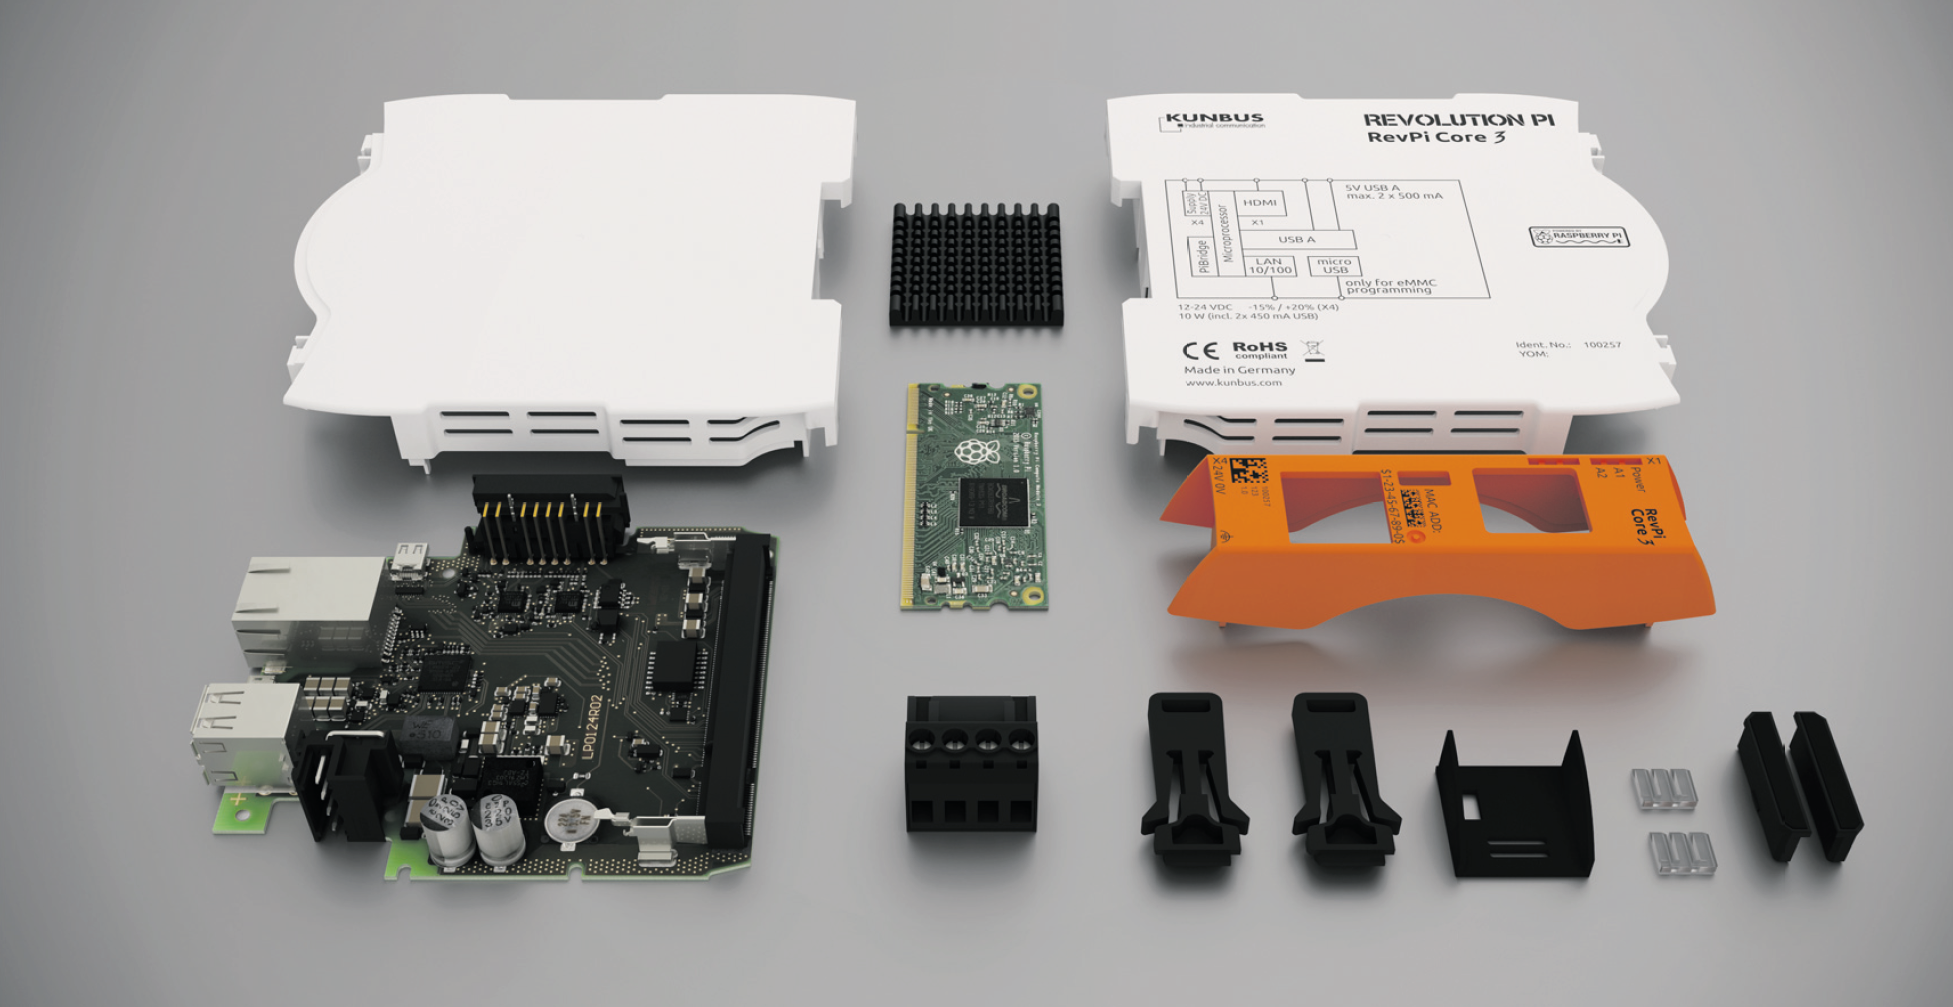
\includegraphics[width=0.85\textwidth]{doc/tex/images/revpi_teardown.png}
    \caption{Der RevPi Core 3 und seine Einzelkomponenten (Quelle: Kunbus)
      \label{fig:revpi-expl}}
\end{figure}

Spezifikationen des RevPi Core 3 \citep[Auswahl, vgl.][S. 1]{datasheet-revpi}:
\begin{itemize}
  \item{Prozessor: BCM2837}
  \item{Taktfrequenz 1,2 GHz}
  \item{Anzahl Prozessorkerne: 4}
  \item{Arbeitsspeicher: 1 GByte}
  \item{eMMC Flash Speicher: 4 GByte}
  \item{Betriebssystem: Angepasstes Raspbian mit RT-Patch}
  \item{RTC mit 24h Pufferung über wartungsfreien Kondensator}
  \item{Treiber / API: Kernel-Treiber schreibt zyklisch Prozessdaten in ein Prozessabbild, Zugriff auf Prozessabbild mittels ioctl-Anfragen oder über Linux-Dateisystem als API zu Fremdsoftware}
  \item{Kommunikationsanschlüsse: 2 x USB 2.0 A, 1 x Micro-USB, HDMI, Ethernet 10/100 Mbit/s}
  \item{Stromversorgung: min. 10,7 V, max. 28,8 V, maximal 10 Watt}
\end{itemize}

Kunbus stellt für den Revolution Pi ein auf Raspbian\footnote{Raspbian ist eine speziell 
für den Raspberry Pi angepasste Variante von Debian.} Stretch basierendes Betriebssystem bereit.
Verwendet wird der Kernel 4.9.76-rt60-v7+ in Verbindung mit dem SMP PREEMPT RT Patch.

\begin{figure}
    \centering
    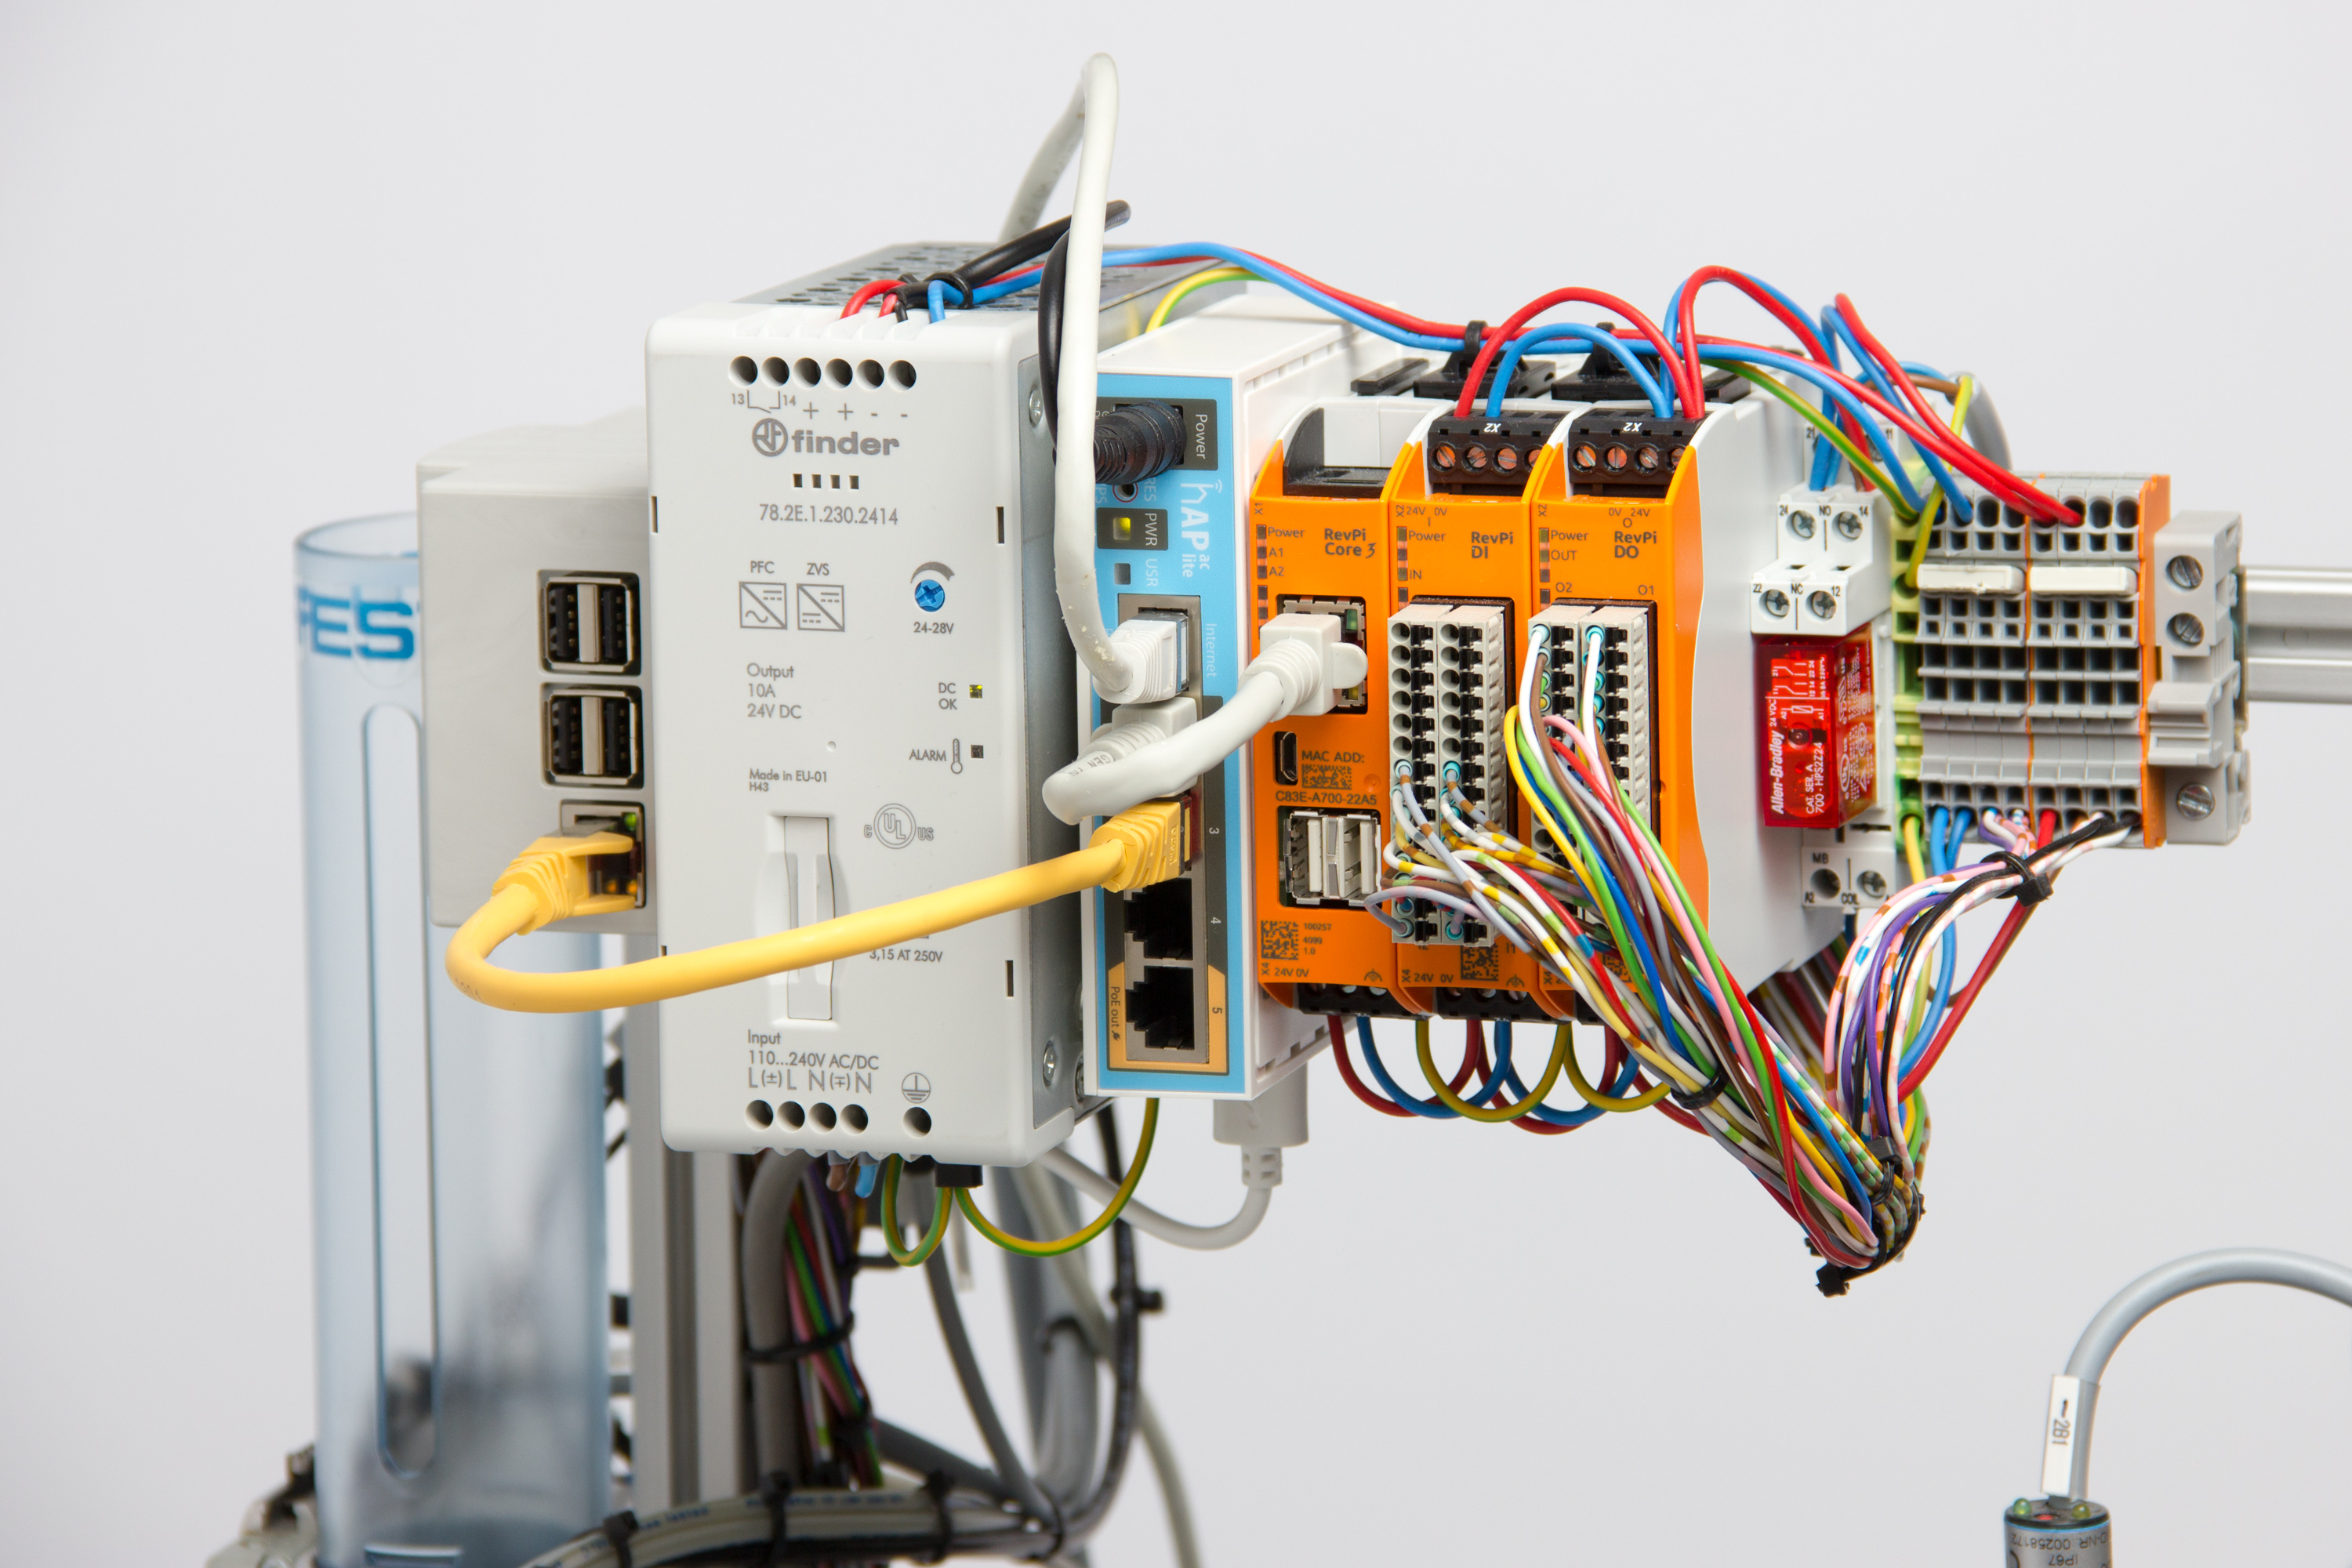
\includegraphics[trim={13cm 5cm 1cm 3cm}, clip, width=0.85\textwidth]{../photos/serverless_plc_img_8}
    \caption{Der Revolution Pi 3 mit digitalen IO-Modulen}
    \label{fig:rev-pi-io}
\end{figure}

Kunbus bietet neben dem sog. Core auch IO- und Gateway-Modulen zur Erweiterung der SPS an, siehe Bild~\ref{fig:rev-pi-io}.
Gateways dienen der Kommunikation mit externen Systemen oder Komponenten
über in der Automatisierungstechnik gängige Protokolle wie PROFIBUS oder EtherCAT. 
IO-Module erlauben die Überwachung und Steuerung von digitalen oder analogen Ein- und Ausgängen (IOs).

Kunbus deklariert die Hardware des Revolution Pi als Open-Source \citep[vgl.][S. 4]{flyer-revpi}. 
Die Schaltpläne des Revolution Pi, genauer die des RevPi Core 3 und der IO-Module, stehen auf der
Website\footnote{\label{downloads}\url{https://revolution.kunbus.com/tutorials/downloads/}} des Herstellers zum 
Download bereit. Eine Lizenz wird nicht angegeben.
Die Raspberry Pi Foundation stellt die Schaltpläne des Compute Modules des weiteren in ihrem Gitub-Repository 
zum Download bereit.

Sowohl die Raspberry Pi Foundation als auch die Kunbus GmbH pflegen aktiv ihre öffentlichen Repositories\footnote{\url{https://github.com/raspberrypi/} resp.~\url{https://github.com/RevolutionPi/}}
auf Github. 

% Kunbus konnte so einige Verbesserungen zum Linux Kernel 4.15 beitragen
% \footnote{siehe \url{https://revolution.kunbus.com/our-contribution-to-linux-4-15/}}.
% \todo{letzten Absatz evtl. weglassen? an sich nicht schlecht, passt aber irgendwie 
% nicht richtig zum Rest und stört den Lesefluss}

\subsubsection{Zugriff auf IO-Module%
        \label{sec:2-io}}
Der Zugriff auf die Ein- und Ausgänge der IO-Module erfolgt über einen RS485-Bus und einen in Form eines Kernel-Moduls bereitgestellten Treiber, genannt piControl. Der RS485-Bus ist über die serielle Schnittstelle des Compute Modules angebunden. 
piControl stellt ein Prozessabbild bereit, welches den physikalischen Zustand der Ein- und Ausgänge der IO-Module repräsentiert.
Das Prozessabbild wird, wie in der Automatisierungstechnik üblich, zyklisch aktualisiert. 
Die angestrebte Zykluszeit beträgt 5ms, kann jedoch je nach Anzahl der angeschlossenen Module auch größer sein. 
Kunbus garantiert bei drei IO-Modulen und zwei Gateway-Modulen eine Zykluszeit von 10 ms \citep[vgl.][]{web-revpi-dio}.
Die garantierte Zykluszeit ermöglicht die Umsetzung von Anwendungen mit harten Echtzeit-Anforderungen.

Fremdanwendungen können über eine Applikationsschnittstelle (API) auf das Prozessabbild zugreifen. 
Hierzu stellt das Kernel-Modul piControl sowohl \lstinline{seek}, \lstinline{read} und \lstinline{write} Methoden zur verfügung, wie auch die Möglichkeit mittels \lstinline{ioctl}-Anfragen gezielt auf einzelne Variablen des Prozessabbildes zuzugreifen.
In der englischsprachigen Wikipedia werden ioctl-Aufrufe wie folgt beschrieben:

\glqq{}The kernel is designed to be extensible, and may accept an extra module called a device driver which runs in kernel space and can directly address the device. An ioctl interface is a single system call by which userspace may communicate with device drivers. [...] The basic kernel can thus allow the userspace to access a device driver without knowing anything about the facilities supported by the device, and without needing an unmanageably large collection of system calls.

[...] ioctl calls provide a convenient way to bridge userspace code to kernel extensions. Kernel extensions can provide a location in the filesystem that can be opened by name, through which an arbitrary number of ioctl calls can be dispatched, allowing the extension to be programmed without adding system calls to the operating system.\grqq{}\citep[vgl.][]{web-wiki-ioctl}

Der Quellcode von piControl steht unter der GNU General Public License Version 2 (GNU GPLv2) und ist 
auf Github verfügbar\footnote{\url{https://github.com/RevolutionPi/piControl}}. Als Einstieg in die 
Entwicklung eigener Steuerungsprogramme liefert Kunbus das C-Programm piTest mit. Dieses verwendet 
piControl und erlaubt dem Nutzer über Kommandozeilen-Parameter die angeschlossenen IO-Module zu steuern.

\begin{figure}[h]
    \centering
    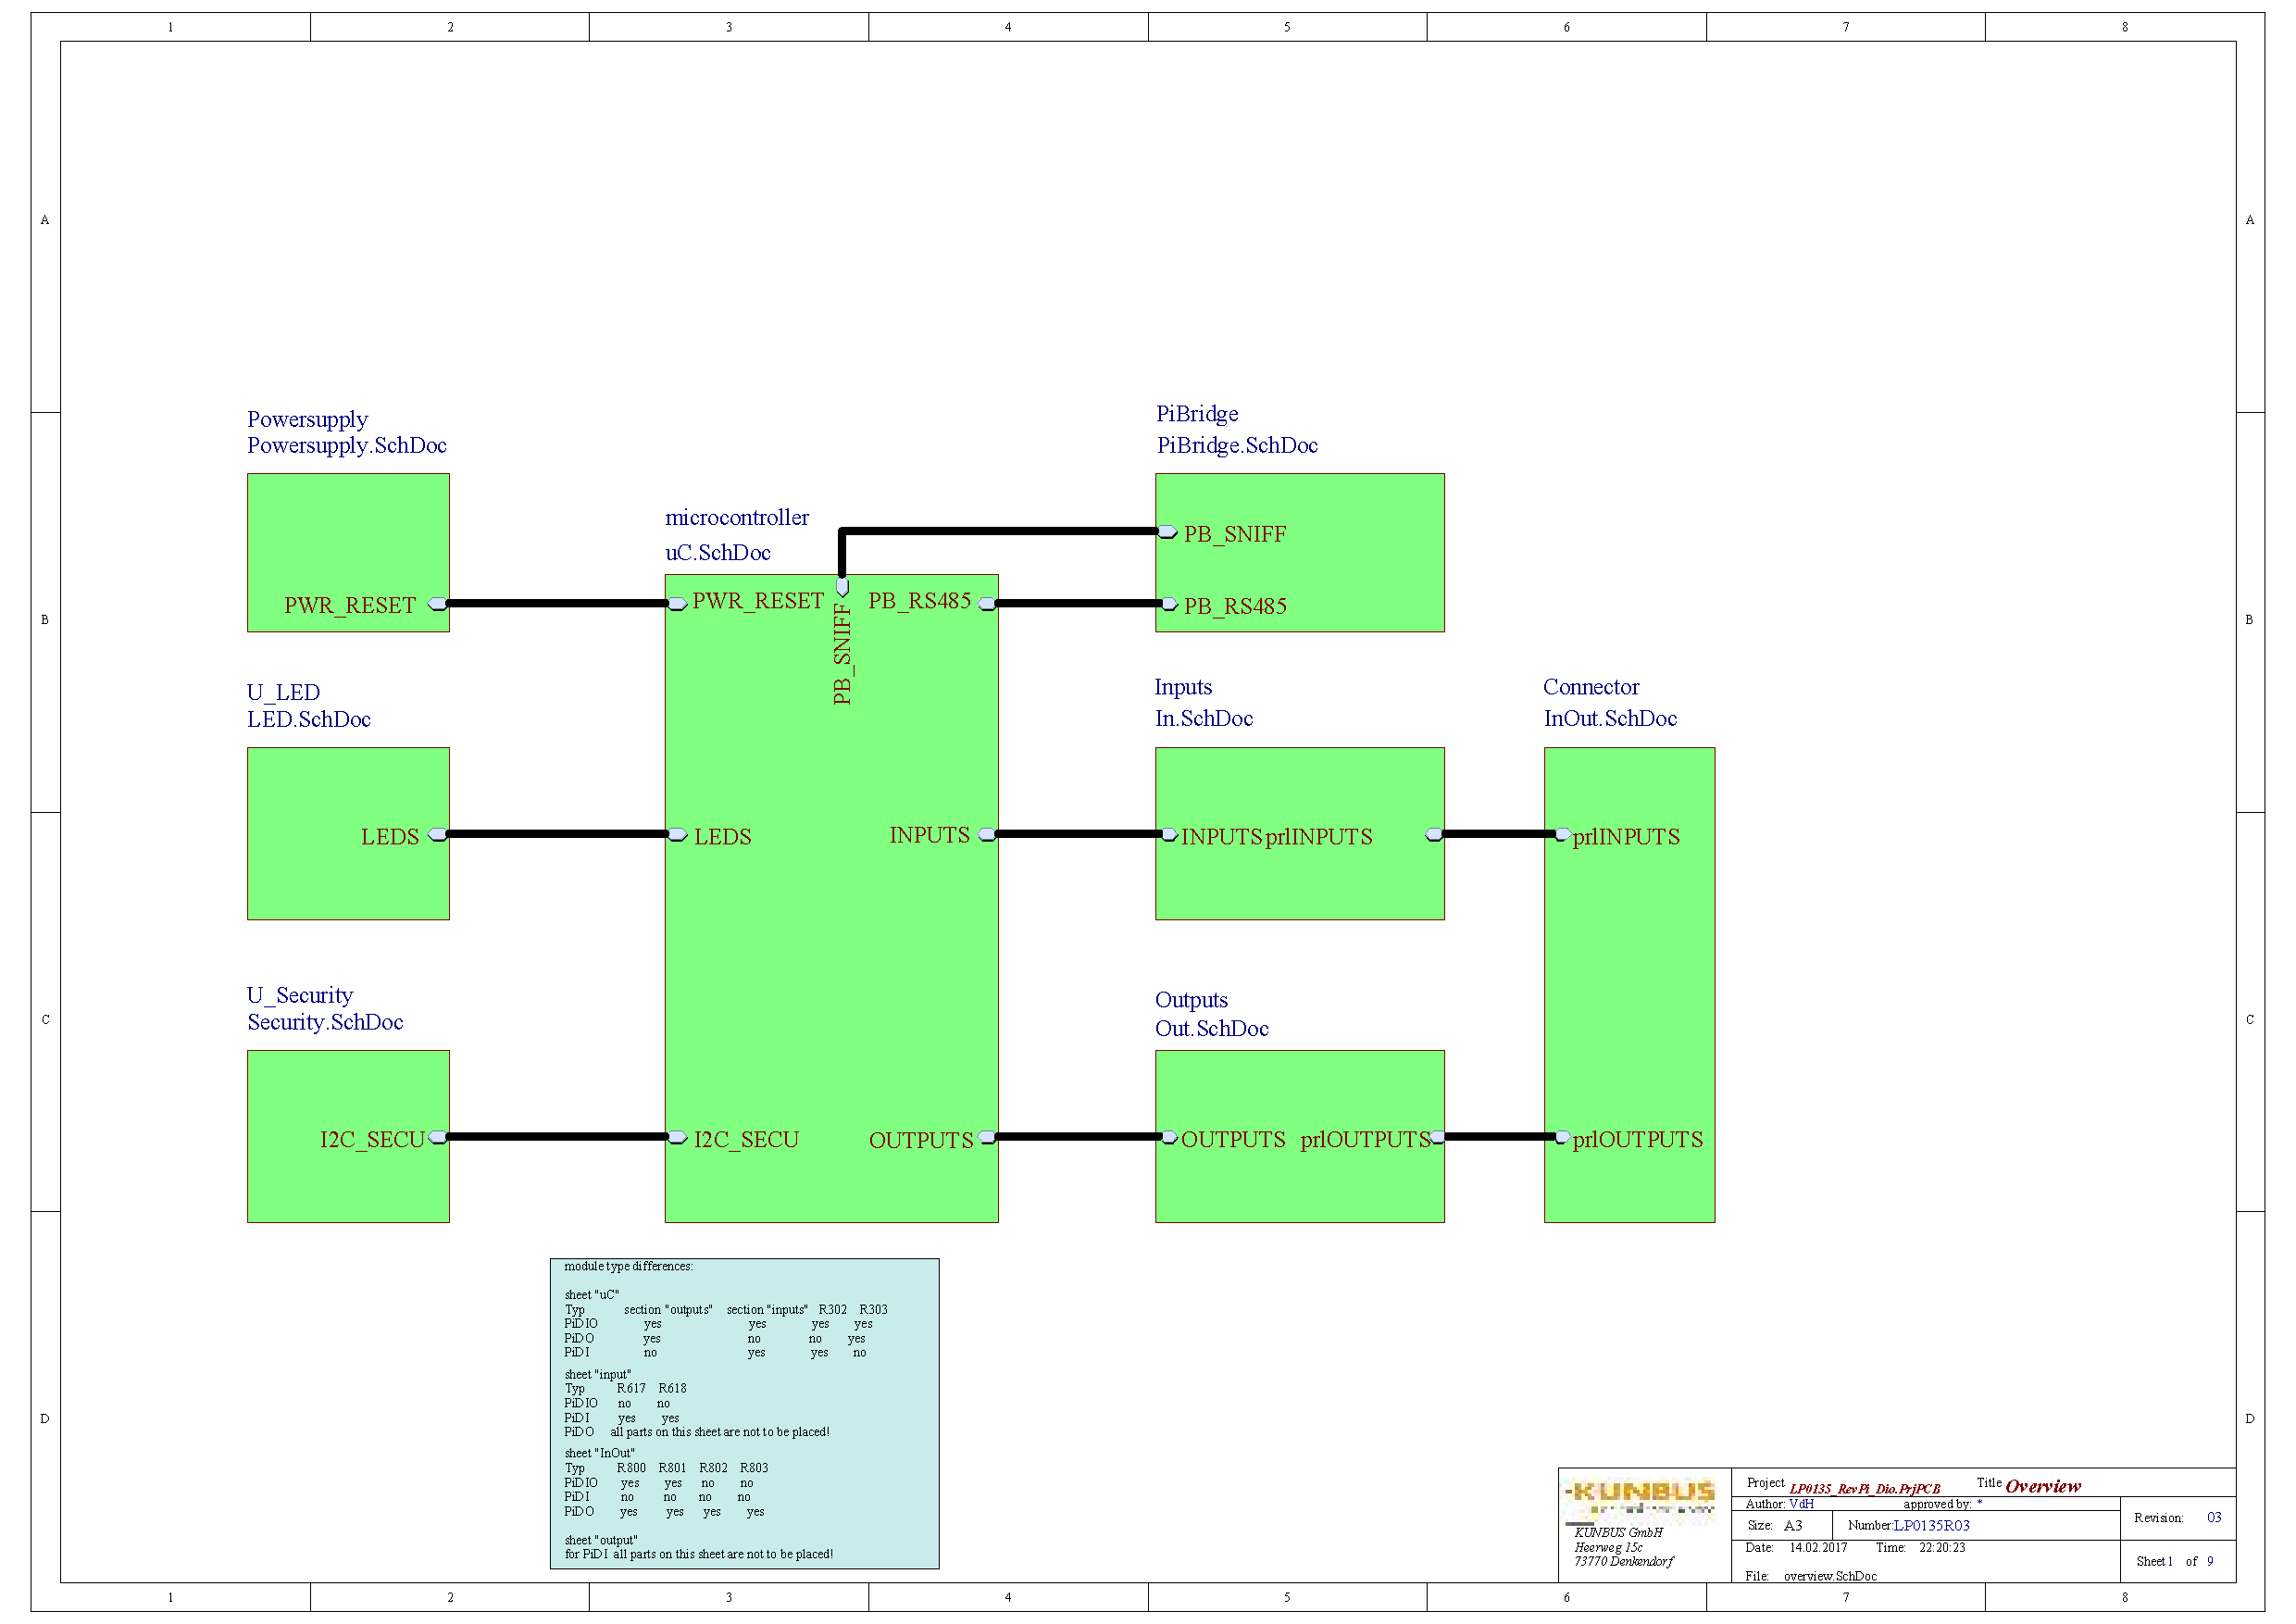
\includegraphics[trim={4cm 7cm 10.5cm 7.3cm}, clip, width=\textwidth]{literature/SchematicPrintsRevPi-DIO}
    \caption{Schematische Darstellung eines DIO-Moduls (Quelle: Kunbus\textsuperscript{\ref{downloads}})
      \label{fig:dio}}
\end{figure}

Jedes der IO-Module stellt ein eigenständiges eingebettetes System dar. Es verfügt
über einen Microcontroller, welcher die IOs bereitstellt und über einen RS485-Bus
mit dem Revolution Pi kommuniziert (siehe Bild~\ref{fig:dio}). 
Kunbus stellt exemplarisch den Quellcode eines DIO-Moduls unter der MIT Lizenz zur
Verfügung\footnote{\url{https://github.com/RevolutionPi/IODeviceExample}}. 


\subsection{Echtzeit und Multitasking unter Linux -- preemptRT und posix%
     \label{sec:2-echtzeit}}
     
Moderne Betriebssysteme realisieren Multitasking i.d.R.\,in Form des präemptiven Multitasking. 
Der Kernel verfügt über einen sog. Scheduler. Dieser priorisiert alle Prozesse und weist ihnen 
Rechenzeit in sog. Time Slots zu. Die Größe der Zeitfenster sowie die Ausführungsreihenfolge 
ist von der Priorität eines Prozesses abhängig. Besonders an einem präemptiven im Gegensatz zu einem kooperativen Scheduler ist dessen Fähigkeit, Tasks während ihrer Ausführung zu unterbrechen bzw. zu pausieren, wenn diese eine bestimmte Dauer überschreiten oder ein höher priorisierter Prozess (bspw. ausgelöst durch einen Interrupt oder durch eine inhärente Periodizität) Rechenleistung benötigt.

Eine Sonderform des präemptiven Multitasking ist das präemptible Multitasking. Hierbei werden auch Teile 
des Kernels als Threads durch den Scheduler ausgeführt. Dieser ist somit in der Lage, auch Prozesse des Kernels
zu unterbrechen, wenn andere Anwendungen Prozessorzeit oder Zugriff auf andere Systemressourcen benötigen
\citep[vgl.][]{web-wiki-praempt}.
     
Der Linux-Kernel implementiert unterschiedliche Präemptions-Modelle \citep[vgl.][/preemption\_models]{web-linuxwiki-basics}:

\begin{itemize}
  \item No Forced Preemption (server):
  Ausgelegt auf maximal möglichen Durchsatz, lediglich Interrupts und
  System-Call-Returns bewirken Präemption.

  \item Voluntary Kernel Preemption (Desktop):
  Neben den implizit bevorrechtigten Interrupts und System-Call-Returns gibt es
  in diesem Modell weitere Abschnitte des Kernels in welchen Preämption explizit
  gestattet ist.

  \item Preemptible Kernel (Low-Latency Desktop):
  In diesem Modell ist der gesamte Kernel, mit Ausnahme sog.~kritischer Abschnitte
  präemptible. Nach jedem kritischen Abschnitt gibt es einen impliziten Präemptions-Punkt.

  \item Preemptible Kernel (Basic RT):
  Dieses Modell ist dem zuvor genannten sehr ähnlich, hier sind jedoch alle Interrupt-Handler
  als eigenständige Threads ausgeführt.

  \item Fully Preemptible Kernel (RT):
  Wie auch bei den beiden zuvor genannten Modellen ist hier der gesamte Kernel
  präemtible. Die Anzahl und Dauer der nicht-präemtiblen kritischen Abschnitte
  ist auf ein notwendiges Minimum beschränkt. Alle Interrupt-Handler sind als
  eigenständige Threads ausgeführt, Spinlocks durch Sleeping-Spinlocks und Mutexe
  durch sog.~RT-Mutexe ersetzt.

\end{itemize}

Lediglich ein präemtibler Kernel kann hartes Echtzeit-Verhalten realisieren, 
da nur hier eine maximale Antwortzeit garantiert werden kann.
Viele Prozesse in der Automatisierungstechnik erfordern harte Echtzeit. 
Eine verspätete Antwort auf eine Anfrage, 
wie etwa das Signal eines Lagenendschalters oder eines Notausschalters kann hier nicht nur über
den Erfolg eines Prozesses, sondern auch über das Leben der daran beteiligten Mitarbeiter entscheiden.
Für weiterführende Erklärungen bzgl.\,Echtzeit, Mutexen und 
Spinlocks sei an dieser Stelle auf die Vorlesung verwiesen~\citep{script-peter}.


\subsubsection{preemptRT%
        \label{sec:2-preemptRT}}

Der Kernel des auf dem Revolution Pi installierten Raspbian mit PREEMP\_RT Patch fällt 
in die Kategorie des \glqq{}Fully Preemptible Kernels\grqq{} (siehe Abschnitt \ref{sec:2-echtzeit}).
Das zugrunde liegende Prinzip lässt sich wie folgt formulieren: Nur Code, welcher absolut nicht-präemtible sein darf, ist es
gestattet nicht-präemtible zu sein. Ziel ist folglich, die Menge des nicht-präemtiblen 
Codes im Linux-Kernel auf das absolut notwendige Minimum zu reduzieren.

Dies wird durch Verwendung folgender Mechanismen erreicht~\citep[vgl.][]{web-linuxwiki-details}:

\begin{itemize}
  \item Hochauflösende Timer
  \item Sleeping Spinlocks
  \item Threaded Interrupt Handlers
  \item rt\_mutex
  \item RCU
\end{itemize}

Diese Mechanismen sind bspw. im Linux-Wiki\footnote{siehe \url{https://wiki.linuxfoundation.org/realtime/documentation/technical_details}} ausführlich beschrieben.

\subsubsection{POSIX%
        \label{sec:2-posix}}
Das Portable Operating System Interface (POSIX) bezeichnet eine Sammlung von Standards, 
welche auf dem Unix-System basieren, jedoch nicht auf dieses beschränkt sind.

Der Wechsel zwischen verschiedenen Unix-Distributionen brachte oft Kompatibilitätsprobleme mit sich. 
Dieser Mangel an Portabilität erschwerte Benutzern und Entwicklern die Verwendung bzw. Bereitstellung 
von Software auf unterschiedlichen Systemen. 
Das Institut für Elektrotechnik und Elektronik (IEEE) begann 1984 mit der Entwicklung des Unix-Standards.
Sie entwickelten das, was heute als Single UNIX Specification bekannt ist und allgemein als POSIX bezeichnet wird~\citep[vgl.][]{web-debianwiki-posix}.
Das Konsortium \glqq{}The Open Group\grqq{} überwacht die weitere Entwicklung dieses Standards.
Ferner stellt es einen Teil der POSIX-Spezifikation frei zur Verfügung~\citep[vgl.][]{web-opengroup-posix}.

Die aktuelle Version POSIX.1-2017 ist verfügbar als IEEE Standard 1003.1-2017 sowie in Form der \glqq{}The Open Group Technical Standard Base Specifications\grqq{}, Ausgabe 7. POSIX.1-2017 definiert eine Standard-Betriebssystemschnittstelle und -umgebung, einschließlich eines Befehlsinterpreters (auch Shell genannt) und gängiger Dienstprogramme zur Unterstützung der Portabilität von Anwendungen auf Quellcode-Ebene. POSIX.1-2017 ist sowohl für Anwendungsentwickler als auch für Systemimplementierer gedacht und umfasst vier Hauptkomponenten \citep[vgl.][]{web-opengroup-overview}:
\begin{itemize}
    \item Basisdefinitionen:\\
          Allgemeine Begriffe, Konzepte und Schnittstellen einschließlich Hilfskonventionen und C-Headern
          
    \item Systemschnittstellen:\\
          Definitionen für Systemdienstfunktionen und Unterprogramme, C-spezifische Systemdienste, Portabilität
        
    \item Shell und Dienstprogramme:\\
          Definitionen für eine Schnittstelle zur Befehlsinterpretation von Diensten und gängige Hilfsprogramme
    
    \item Begründungen und Historie
\end{itemize}

Debian basiert auf Linux und verwendet den Linux-Kernel. Linux ist zu großen Teilen POSIX-kompatibel. Debian ist jedoch nicht POSIX-zertifiziert, da diese Zertifizierung mit hohen Kosten verbunden ist\citep[vgl.][Kapitel 4.4.]{web-debian-faq}.

Beide Kernkomponenten des in dieser Arbeit vorgestellten Projektes nutzen Komponenten von Linux, 
welche an den POSIX-Standard angelehnt sind: open62541 verwendet u.a.\,POSIX-Threads und
Mutexe~\citep[vgl.][pthread.h]{web-opengroup-pthread}, piControl nutzt POSIX-Semaphoren
\citep[vgl.][semaphore.h]{web-opengroup-semaphore}. 


\subsection{OPC-UA und open62541%
     \label{sec:2-opc}}
In diesem Abschnitt sollen Möglichkeiten des Datenaustausch zwischen Komponenten der
Automatisierungstechnik vorgestellt werden. OPC-UA stellt einen offenen, IP-basierten Kommunikationsstandard
für Sensoren und Steuerungen dar. open62541 ist eine freie Client- sowie Server-Implementierung dieses
Standards, geschrieben in C.


\subsubsection{OPC UA%
        \label{sec:2-opcua}}

Open Platform Communications (OPC) ist eine Familie von Standards zur herstellerunabhängigen
Kommunikation von Maschinen (M2M) in der Automatisierungstechnik. Die sog. OPC Task Force, zu deren
Mitgliedern verschiedene etablierte Firmen der Automatisierungsindustrie gehören, veröffentlichte
die OPC Specification Version 1.0 im August 1996.
Motiviert ist dieser offene Standard durch die Erkenntniss, dass die Anpassung der
zahlreichen Herstellerstandards an individuelle Infrastrukturen und Anlagen einen
großen Mehraufwand verursachen.
Die Wikipedia beschreibt das Anwendungsgebiet für OPC wie folgt \citep[vgl.][]{web-wiki-opc}:

\glqq{}OPC wird dort eingesetzt, wo Sensoren, Regler und Steuerungen verschiedener Hersteller
ein gemeinsames Netzwerk bilden. Ohne OPC benötigten zwei Geräte zum Datenaustausch
genaue Kenntnis über die Kommunikationsmöglichkeiten des Gegenübers. Erweiterungen
und Austausch gestalten sich entsprechend schwierig. Mit OPC genügt es, für jedes
Gerät genau einmal einen OPC-konformen Treiber zu schreiben. Idealerweise wird
dieser bereits vom Hersteller zur Verfügung gestellt. Ein OPC-Treiber lässt sich
ohne großen Anpassungsaufwand in beliebig große Steuer- und Überwachungssysteme
integrieren.

OPC unterteilt sich in verschiedene Unterstandards, die für den jeweiligen Anwendungsfall
unabhängig voneinander implementiert werden können. OPC lässt sich damit verwenden
für Echtzeitdaten (Überwachung), Datenarchivierung, Alarm-Meldungen und neuerdings
auch direkt zur Steuerung (Befehlsübermittlung).\grqq{}

OPC basiert in der ursprünglichen Spezifikation (auch als OPC DA bezeichnet) auf Microsofts DCOM-Spezifikation.
DCOM macht Funktionen und Objekte einer Anwendung anderen Anwendungen im Netzwerk
zugänglich. Der OPC-Standard definiert entsprechende DCOM-Objekte um mit anderen
OPC-Anwendungen Daten austauschen zu können. Die Verwendung von DCOM bindet Anwender
jedoch an Betriebssysteme von Microsoft. 

\begin{figure}
    \centering
    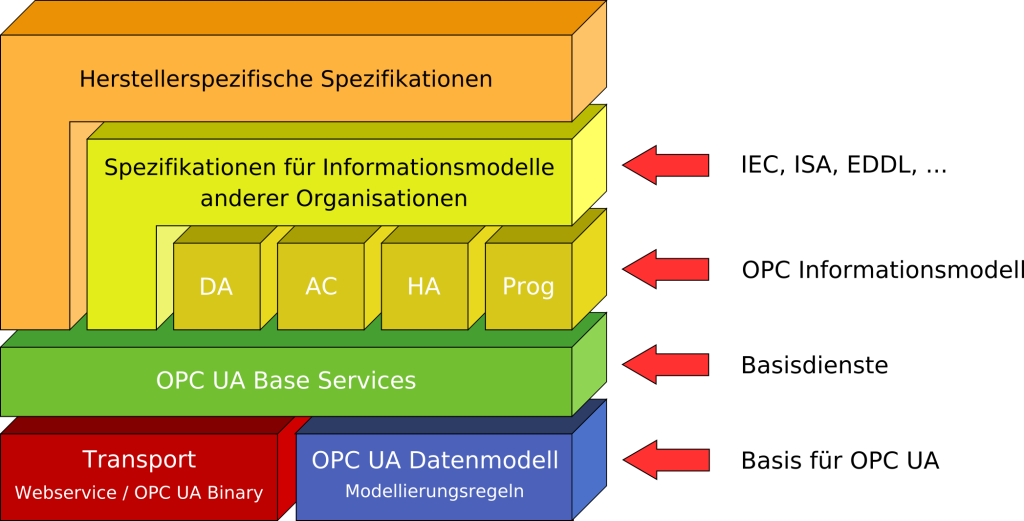
\includegraphics[width=0.85\textwidth]{images/UA_Architecture_1024.png}
    \caption{Die OPC Unified Architecture. Grafik von Gerhard Gappmeier - ascolab GmbH, CC BY-SA 3.0}
    \label{fig:opc-unified-architecture}
\end{figure}
% Evtl Grafik: Von Gerhard Gappmeier - ascolab GmbH, CC BY-SA 3.0, https://de.wikipedia.org/w/index.php?curid=1892069

Die ursprüngliche OPC Spezifikation wurde 2006 durch die Entwicklung der 
OPC Unified Architecture (OPC UA) überholt. 
Diese zeichnet sich durch eine Service-orientierte Architektur (SOA) aus, deren Struktur
aus mehreren Schichten besteht, siehe Abbilung~\ref{fig:opc-unified-architecture}. 
Über der untersten Schicht, dem Betriebssystem des Servers, verbindet eine Portabilitäts-Schicht 
den sog.\, UA ANSI C Stack mit einer API. Diese API kann bspw.\,in C++ geschrieben sein, 
und erlaubt die Anbindung der obersten Schicht, der Anwendungsschicht~\citep[vgl.][]{web-spec-opc}.
OPC UA setzt auf einem eigenen Kommunikationsstack auf; die Verwendung von DCOM
und damit die Bindung an Microsoft wurden aufgelöst.

Neben Architektur und Kommunikationsschnittstellen wird in der OPC Spezifikation auch ein 
Informationsmodell definiert. Die deutschsprachige Wikipedia beschreibt dieses wie folgt: 

\glqq{}Das OPC[-UA]-Informationsmodell ist nicht mehr nur eine Hierarchie aus Ordnern, Items
und Properties. Es ist ein sogenanntes Full-Mesh-Network aus Nodes, mit dem neben
den Nutzdaten eines Nodes auch Meta- und Diagnoseinformationen repräsentiert werden. [...]
Ein Node ähnelt einem Objekt aus der objektorientierten Programmierung. Ein Node
kann Attribute besitzen, die gelesen werden können. Es ist möglich Methoden zu definieren und aufzurufen. [...]
Weiterhin werden Events unterstützt, die versendet werden können
(AE (Alarms \& Events), DA DataChange), um bestimmte Informationen zwischen Geräten
auszutauschen. Ein Event besitzt unter anderem einen Empfangszeitpunkt, eine Nachricht
und einen Schweregrad. Die o.\,g. Nodes werden sowohl für die Nutzdaten als auch
alle anderen Arten von Metadaten verwendet. Der damit modellierte OPC-Adressraum
beinhaltet nun auch ein Typmodell, mit dem sämtliche Datentypen spezifiziert werden.\grqq{}


\subsubsection{open62541%
        \label{sec:2-open62541}}
open62541 ist eine offene und freie Implementierung von OPC UA. 
Die in C geschriebene Bibliothek stellt eine beständig zunehmende Anzahl der im OPC UA Standard definierten
Funktionen bereit. Sie kann sowohl zur Erstellung von OPC-Servern als auch von -Clients
genutzt werden. Ergänzend zu der unter der Mozilla Public License v2.0 lizensierten
Bibliothek stellt das open62541 Projekt auch Beispielprogramme unter einer CC0 Lizenz
zur Verfügung.
Zu den Unterstützern des Projektes zählen u.a.\, die RWTH Aachen, das Frauenhofer IOSB sowie die TU Dresden.

Die Bibliothek eignet sich auch für die Entwicklung auf eingebetteten Systemen und
Microcontrollern. Die Größe einer Server-Binary kann weniger als 100kB betragen.

Folgende Auswahl an Eigenschaften und Funktionen zeichnet die in dieser Arbeit verwendete
Version 0.3 von open62541 aus:
\begin{itemize}
  \item Kommunikationionsstack
  \begin{itemize}
      \item OPC UA Binär-Protokoll (HTTP oder SOAP werden gegenwärtig nicht unterstützt)
      \item Austauschbare Netzwerk-Schicht, welche die Verwendung eigener Netzwerk-APIs
      erlaubt.
      \item Verschlüsselte Kommunikationion
      \item Asynchrone Dienst-Anfragen im Client
  \end{itemize}
  \item Informationsmodell
  \begin{itemize}
    \item Unterstützung aller OPC UA Node-Typen, inkl.~Methoden
    \item Hinzufügen und Entfernen von Nodes und Referenzen zur Laufzeit.
    \item Vererbung und Instanziierung von Objekt- und Variablentypen
    \item Zugriffskontrolle auch für einzelne Nodes
  \end{itemize}
  \item Subscriptions
  \begin{itemize}
    \item Erlaubt die Überwachung (subscriptions / monitoreditems)
    \item Sehr geringer Ressourcenbedarf pro überwachtem Wert
  \end{itemize}
  \item Code-Generierung auf XML-Basis
  \begin{itemize}
    \item Erlaubt die Erstellung von Datentypen
    \item Erlaubt die Generierung des serverseitigen Informationsmodells
  \end{itemize}
\end{itemize}

Weiterführende Informationen und Code-Beispiele bietet die ausführliche Dokumentation des Projektes~\citep[siehe]{web-open62541} sowie der kommentierte Quelltext.

% % % Imports nur für Referenzenauflösung während des Schreibens! Vorm Kompilieren auskommentieren!
% \bibliography{0_hauptdatei}
% \input{1_einleitung}
% \input{2_grundlagen}
% \input{3_konzeption}
% \input{4_implementierung}
% \input{5_tests}
% \input{6_zusammenfassung}
% \input{anhang}
% % Ende Imports

\section{Systemkonzept%
  \label{sec:3-konzeption}}
Auf Basis der in Abschnitt [...] vorgestellten Möglichkeiten folgt nun die Ausarbeitung eines Konzepts.

\subsection{Anbindung der IO an den OPC-Server%
     \label{sec:3-anbindung}}

\subsection{Integration des OPC-Servers in das System%
     \label{sec:3-integration}}

% % % Imports nur für Referenzenauflösung während des Schreibens! Vorm Kompilieren auskommentieren!
% \bibliography{0_hauptdatei}
% \input{1_einleitung}
% \input{2_grundlagen}
% \input{3_konzeption}
% \input{4_implementierung}
% \input{5_tests}
% \input{6_zusammenfassung}
% \input{anhang}
% % Ende Imports

\section{Implementierung%
  \label{sec:4-implementierung}}
Das folgende Kapitel stellt in Auszügen die Implementierung des OPC-Servers sowie die Anbindung an die IO-Module
der SPS dar. Der Schwerpunkt liegt hierbei auf der Funktionsweise des piControl-Treibers und dessen Integration in das Projekt. Abschnitt~\ref{sec:4-picontrol} erklärt die zum Schreibens eines Bits verwendeten Funktionsaufrufe.
Zuvor soll jedoch in Abschnitt~\ref{sec:4-open62541} der Teil des OPC-Servers vorgestellt werden, welcher auf besagten Treiber zugreift. 

\subsection{Implementierung des OPC-Servers%
     \label{sec:4-open62541}}
Wie im vorangegangenen Abschnitt~\ref{sec:3-integration} begründet, soll die Verknüpfung zwischen dem Prozessabbild der SPS und den auf dem OPC-Server bereitgestellten Werten über sog.\,Datenquellen erfolgen. Hierzu ist zunächst eine Callback-Methode zu implementieren, welche bei einem Lese- oder Schreibzugriff auf eine Variable aufgerufen wird. Die Verknüpfung zwischen Callback-Methode und Variable muss manuell erfolgen.

\begin{lstlisting}[language={c},firstnumber=237,caption={Auszug der Methode \lstinline{linkDataSourceVariable} in \lstinline{variables.c}\label{lst:4-linkDataSourceVariable}}]
extern UA_StatusCode
 linkDataSourceVariable(UA_Server *server, UA_NodeId nodeId) {
     bool readonly = false;
     UA_DataSource dataSourceVariable;
     UA_StatusCode rc; |>\setcounter{lstnumber}{254}<|

     dataSourceVariable.read = readDataSourceVariable;
     if (!readonly)
        dataSourceVariable.write = writeDataSourceVariable;
     else
        dataSourceVariable.write = writeReadonlyDataSourceVariable;

     return UA_Server_setVariableNode_dataSource(server, nodeId, dataSourceVariable);
 }
\end{lstlisting}

\begin{figure}[h]
    \centering
    \includegraphics[width=0.42\textwidth]{doc/img/OPC_RevPiDO.pdf}
    \caption{Auszug des verwendeten Nodesets, hier Digitalausgang 1 des Versuchsaufbaus
      \label{fig:opc-do}}
\end{figure}

Die in Listing~\ref{lst:4-linkDataSourceVariable} abgebildete Methode \lstinline{linkDataSourceVariable()} erzeugt ein Struct vom Typ \lstinline{UA_DataSource}. In diesem werden dem Lesen und Schreiben einer OPC-Variablen entsprechende Callback-Methoden zugewiesen. Die Verknüpfung einer OPC-Variable, genauer ihrer NodeId, mit der zuvor definierten Datenquelle erfolgt über die von open62541 bereitgestellte Methode \lstinline{UA_Server_setVariableNode_dataSource()}. Vor dem Lesen und nach dem Schreiben dieser Variable werden von nun an die entsprechenden Callbacks aufgerufen.
     
\begin{lstlisting}[language={c},firstnumber=168,caption={Auszug des Callbacks \lstinline{writeDataSourceVariable} in \lstinline{variables.c}\label{lst:4-writeDataSourceVariable}}]  
extern UA_StatusCode
 writeDataSourceVariable(UA_Server *server,
            const UA_NodeId *sessionId, void *sessionContext,
            const UA_NodeId *nodeId, void *nodeContext,
            const UA_NumericRange *range, const UA_DataValue *dataValue) {

    UA_StatusCode retval  = UA_STATUSCODE_GOOD;
    UA_NodeId *nameNodeId = UA_malloc(sizeof(UA_NodeId));
    UA_QualifiedName nameQN = UA_QUALIFIEDNAME(1, "Name");
    UA_Variant nameVar;
    UA_Boolean bit;

    retval |= findSiblingByBrowsename(server, nodeId, &nameQN, nameNodeId);
    retval |= UA_Server_readValue(server, *nameNodeId, &nameVar);
    retval |= UA_Boolean_copy(dataValue->value.data, &bit);

    |>\tikzmarkin[set border color=martinired]{writeIO}<|PI_writeSingleIO(String_fromUA_String(nameVar.data), &bit, false);                                                 |>\tikzmarkend{writeIO}<|

    free(nameNodeId);
    return retval;
 }
\end{lstlisting}

Listing~\ref{lst:4-writeDataSourceVariable} zeigt die Callback-Methode, welche nach dem Schreiben einer Variablen auf dem OPC-Server aufgerufen wird.
Dieser Methode wird neben der NodeId der mit ihr verknüpften Variablen auch der Wert dieser in Form eines Zeigers auf ein Struct vom Typ \lstinline{UA_DataValue} übergeben.

Die Gestaltung des hier verwendeten Nodesets sieht vor, dass in einer OPC-Variablen \lstinline{"Name"} der Bezeichner des zu schreibenden Digitalausgangs hinterlegt ist, siehe Abbildung~\ref{fig:opc-do}. Dies erlaubt eine Rekonfiguration der Ein- und Ausgänge der SPS ohne Änderungen im Programmcode des OPC-Servers vornehmen zu müssen.
Es ist daher erforderlich, nach jedem Schreiben einer mit einem Digitalausgang verknüpften Variablen, hier \lstinline{"Value"}, dessen Bezeichner \lstinline{"Name"} abzufragen. 
Dies geschieht in den Zeilen 180 und 181.
Anschließend wird dieser Bezeichner sowie der zu schreibende Wert der Methode \lstinline{PI_writeSingleIO()} übergeben, welche wiederum die Interaktion mit piControl übernimmt (vgl. Abschnitt \ref{sec:4-picontrol}).
 
\subsection{Integration von piControl%
     \label{sec:4-picontrol}}
In Abschnitt~\ref{sec:2-io} wurde die Anbindung der IO-Module des Revolution Pi sowie die Funktionsweise von piControl aus Anwendersicht beschrieben. Die verfügbare Literatur beschränkt sich auch auf lediglich diese Sicht; eine weiterführende Dokumentation für Entwickler gibt es, neben der in Abschnitt~\ref{sec:3-anbindung} vorgestellten Manpage, nicht. 
In diesem Abschnitt soll daher der Quellcode von piControl sowie dessen Verwendung im Projekt genauer betrachtet werden.
Hierzu wird exemplarisch die in Abschnitt~\ref{sec:4-open62541} eingeführte Methode \lstinline{PI_writeSingleIO()} untersucht.
Diese Methode ermöglicht das Setzen eines einzelnen Bits im Prozessabbild der SPS, und damit das Schalten eines digitalen Ausgangs auf einem IO-Modul.
Die äquivalente Methode \lstinline{int piControlGetBitValue(SPIValue *pSpiValue)} zum Lesen eines Bits bzw. Eingangs funktioniert analog und soll daher an dieser Stelle nicht dediziert erörtert werden.

\begin{lstlisting}[language={c},firstnumber=97,
                   caption={Setzen eines phsikalischen, digitalen Ausgangs in \lstinline{revpi.c}
                   \label{lst:4-PI_writeSingleIO}}]
extern void PI_writeSingleIO(char *pszVariableName, bool *bit, bool verbose)
{
	int rc;
	SPIVariable sPiVariable;
	SPIValue sPIValue;

	strncpy(sPiVariable.strVarName, pszVariableName, sizeof(sPiVariable.strVarName));
	rc = piControlGetVariableInfo(&sPiVariable);
	if (rc < 0) {
		printf("Cannot find variable '%s'\n", pszVariableName);
		return;
	}

		sPIValue.i16uAddress = sPiVariable.i16uAddress;
		sPIValue.i8uBit = sPiVariable.i8uBit;
		sPIValue.i8uValue = *bit;
		rc = |>\tikzmarkin[set border color=martinired]{setBitValue}<|piControlSetBitValue(&sPIValue)|>\tikzmarkend{setBitValue}<|;
		if (rc < 0)
			printf("Set bit error %s\n", getWriteError(rc));
		else if (verbose)
			printf("Set bit %d on byte at offset %d. Value %d\n", sPIValue.i8uBit, sPIValue.i16uAddress,
			       sPIValue.i8uValue);
}
\end{lstlisting}

Der Programmcode in Listing~\ref{lst:4-PI_writeSingleIO} ist Teil des implementierten OPC-Servers. In diesem wird auf zwei Funktionen des piControl-Treibers zugegriffen. 
Beiden Methoden wird als Argument ein Zeiger auf ein Struct vom Typ \lstinline{SPIValue} übergeben. Der im Struct abgelegte Name wird mittels \lstinline{piControlGetVariableInfo(&sPIValue)} zu einer Adresse im Prozessabbild aufgelöst. Diese wird in \lstinline{sPIValue.i16uAdress} gespeichert. Der Wert der Variablen wird anschließend mittels \lstinline{piControlSetBitValue(&sPIValue)} an dieser Adresse in das Prozessabbild geschrieben.

\begin{lstlisting}[language={c},firstnumber=309,caption={Methode \lstinline{piControlSetBitValue} in \lstinline{piControlIf.c}\label{lst:4-piControlSetBitValue}}]
int |>\tikzmarkin[set border color=martiniblue]{setBitValueFcn}<|piControlSetBitValue(SPIValue *pSpiValue)|>\tikzmarkend{setBitValueFcn}<|
{
    piControlOpen();

    if (PiControlHandle_g < 0)
	    return -ENODEV;

    pSpiValue->i16uAddress += pSpiValue->i8uBit / 8;
    pSpiValue->i8uBit %= 8;

    if (|>\tikzmarkin[set border color=martinired]{ioctl}<|ioctl(PiControlHandle_g, KB_SET_VALUE, pSpiValue)|>\tikzmarkend{ioctl}<| < 0)
	    return errno;

    return 0;
}
\end{lstlisting}

Die in Listing~\ref{lst:4-piControlSetBitValue} dargestellte Methode \lstinline{piControlSetBitValue} ist lediglich eine Hüllfunktion (häufig auch als Wrapper-Funktion bezeichnet) für einen Aufruf des \lstinline{ioctl} Kernel-Moduls.
Folgende Parameter werden übergeben:
\lstinline{PiControlHandle_g} ist die Referenz auf die Geräte-Datei des piControl-Treibers. \lstinline{KB_SET_VALUE} ist das ioctl-Kommando zum Schreiben eines Bits in das Prozessabbild. Der Zeiger \lstinline{pSpiValue} verweist auf ein Struct des bereits vorgestellten Typs \lstinline{SPIValue}.

\begin{lstlisting}[language={c},firstnumber=80,caption={Methode \lstinline{piControlOpen} in \lstinline{piControlIf.c}\label{lst:4-piControlOpen}}]
void piControlOpen(void)
{
    /* open handle if needed */
    if (PiControlHandle_g < 0)
    {
	    |>\tikzmarkin[set border color=martiniblue]{PiControlHandle}<|PiControlHandle_g = open(PICONTROL_DEVICE, O_RDWR)|>\tikzmarkend{PiControlHandle}<|;
    }
}
\end{lstlisting}

Die in Listing~\ref{lst:4-piControlOpen} dargestellte Methode öffnet, sofern nicht bereits geschehen, die Geräte-Datei. Das Macro \lstinline{PICONTROL_DEVICE} verweist hierbei auf \lstinline{/dev/piControl0}.

\begin{lstlisting}[language={c},firstnumber=721,caption={Methode \lstinline{piControlIoctl} in \lstinline{piControlMain.c}\label{lst:4-piControlIoctl}}]
static long |>\tikzmarkin[set border color=martiniblue, below offset=0.9em]{piControlIoctl}<|piControlIoctl(struct file *file, unsigned int prg_nr, 
                           unsigned long usr_addr)                                      |>\tikzmarkend{piControlIoctl}<|
{
  int status = -EFAULT;
  tpiControlInst *priv;
  int timeout = 10000;	// ms

  if (prg_nr != KB_CONFIG_SEND && prg_nr != KB_CONFIG_START && !isRunning()) {
  	return -EAGAIN;
  }

  priv = (tpiControlInst *) file->private_data;

  if (prg_nr != KB_GET_LAST_MESSAGE) {
  	// clear old message
  	priv->pcErrorMessage[0] = 0;
  }

  switch (prg_nr) {|>\setcounter{lstnumber}{864}<|

    case |>\tikzmarkin[set border color=martiniblue]{KB_SET_VALUE}<|KB_SET_VALUE:|>\tikzmarkend{KB_SET_VALUE}<|
  		{
  			SPIValue *pValue = (SPIValue *) usr_addr;

  			if (!isRunning())
  				return -EFAULT;

  			if (pValue->i16uAddress >= KB_PI_LEN) {
  				status = -EFAULT;
  			} else {
  				INT8U i8uValue_l;
  				my_rt_mutex_lock(&piDev_g.lockPI);
  				i8uValue_l = piDev_g.ai8uPI[pValue->i16uAddress];

  				if (pValue->i8uBit >= 8) {
  					i8uValue_l = pValue->i8uValue;
  				} else {
  					if (pValue->i8uValue)
  						i8uValue_l |= (1 << pValue->i8uBit);
  					else
  						i8uValue_l &= ~(1 << pValue->i8uBit);
  				}

  				|>\tikzmarkin[set border color=martinired]{i8uValue}<|piDev_g.ai8uPI[pValue->i16uAddress] = i8uValue_l;|>\tikzmarkend{i8uValue}<|
  				rt_mutex_unlock(&piDev_g.lockPI);

  #ifdef VERBOSE
  				pr_info("piControlIoctl Addr=%u, bit=%u: %02x %02x\n", pValue->i16uAddress, pValue->i8uBit, pValue->i8uValue, i8uValue_l);
  #endif

  				status = 0;
  			}
  		}
  		break; |>\setcounter{lstnumber}{1314}<|

    default:
      pr_err("Invalid Ioctl");
      return (-EINVAL);
      break;

    }

    return status;
  }
\end{lstlisting}

Listing~\ref{lst:4-piControlIoctl} zeigt in Auszügen die ioctl-Methode des piControl Kernel-Treibers. Diese bekommt folgende Argumente übergeben: \lstinline{struct file *file} enthält den Verweis auf die Geräte-Datei, hier \lstinline{/dev/piControl0}. Der Wert von \lstinline{unsigned int prg_nr} beschreibt die Anfrage an den Treiber, in diesem Fall \lstinline{KB_SET_VALUE}. Das Argument \lstinline{unsigned long usr_addr} enthält einen typ-agnostischen Pointer. Dieser verweist auf einen Speicherbereich, in welchem die zur Bearbeitung der Anfrage notwendigen Daten abgelegt sind. Hier können auch vom Treiber empfangene Daten dem Anwendungsprogramm bereitgestellt werden. 

Die switch-case-Anweisung führt die über das Argument \lstinline{prg_nr} spezifizierte Aktion aus. Hier betrachten wir \lstinline{KB_SET_VALUE}:
Zunächst wird in Zeile 868 der übergebene Zeiger \lstinline{usr_addr} mittels explizitem Typecast zu einem Zeiger des Typs \lstinline{SPIValue *} konvertiert. Da dieser auf Daten im Userspace verweist, ist beim Zugriff durch den Kernel-Treiber besondere Vorsicht geboten.
In Zeile 877 wird mittels Mutex das Prozessabbild \lstinline{piDev_g} für den Zugriff durch andere Threads oder Prozesse gesperrt.
\lstinline{my_rt_mutex_lock} verweist hierbei auf die Funktion \lstinline{rt_mutex_lock} aus \lstinline{linux/sched.h}\footnote{Offenbar wurde hier auch eine alternative Implementierung vorgesehen, siehe revpi\_common.h}

In Zeile 889 wird das Byte \lstinline{i8uValue_l}, welches den zu schreibenden Wert enthält in das Prozessabbild übertragen. Anschließend wird die Mutex auf \lstinline{piDev_g} wieder entsperrt.
\newpage

\begin{lstlisting}[language={c},firstnumber=62,caption={Auszug des Struct \lstinline{spiControlDev} in \lstinline{piControlMain.h}\label{lst:4-spiControlDev}}]
|>\tikzmarkin[set border color=martiniblue]{spiControlDev}<|typedef struct spiControlDev|>\tikzmarkend{spiControlDev}<| {
	// device driver stuff
	int init_step;
	enum revpi_machine machine_type;
	void *machine;
	struct cdev cdev;	// Char device structure
	struct device *dev;
	struct thermal_zone_device *thermal_zone;

	|>\tikzmarkin[set border color=martiniblue]{processImage}<|// process image stuff
	INT8U ai8uPI[KB_PI_LEN];
	INT8U ai8uPIDefault|>\tikzmarkin[set border color=martinired]{KB_PI_LEN_0}<|[KB_PI_LEN]|>\tikzmarkend{KB_PI_LEN_0}<|;
	struct rt_mutex lockPI;        |>\tikzmarkend{processImage}<|
	bool stopIO;
	piDevices *devs; |>\setcounter{lstnumber}{94}<|
} tpiControlDev;
\end{lstlisting}

Das Prozessabbild ist als Byte-Array der Länge \lstinline{KB_PI_LEN} in Listing~\ref{lst:4-spiControlDev} definiert. Konfigurationsparameter wie \lstinline{KB_PI_LEN} oder die Zykluszeit für den Datenaustausch zwischen SPS und IO-Modulen sind im folgenden Listing~\ref{lst:4-process} definiert.

\begin{lstlisting}[language={c},firstnumber=119,caption={Konfigurationsparameter des Prozessabbildes in project.h\label{lst:4-process}}]
#define INTERVAL_PI_GATE (5*1000*1000)  // 5 ms piGateCommunication |>\setcounter{lstnumber}{128}<|

#define INTERVAL_IO_COM (5*1000*1000)  // 5 ms piIoComm |>\setcounter{lstnumber}{132}<|

#define KB_PD_LEN       512
|>\tikzmarkin[set border color=martiniblue]{KB_PI_LEN_1}<|#define KB_PI_LEN       4096|>\tikzmarkend{KB_PI_LEN_1}<|
\end{lstlisting}

Das zu setzende Bit wurde zu diesem Zeitpunkt erfolgreich in das Prozessabbild der SPS geschrieben.
Es stellt sich die Frage, wie dieses nun an das IO-Modul kommuniziert wird.
Die Kommunikation mit allen angebundenen Modulen ist ebenfalls Aufgabe des piControl-Treibers.

\begin{lstlisting}[language={c},firstnumber=256,caption={Auszug der Methode \lstinline{piIoThread} in \lstinline{revpi_core.c}\label{lst:4-piIoThread}}]
static int piIoThread(void *data)
{
	//TODO int value = 0;
	ktime_t time;
	ktime_t now;
	s64 tDiff;

	hrtimer_init(&piCore_g.ioTimer, CLOCK_MONOTONIC, HRTIMER_MODE_ABS);
	piCore_g.ioTimer.function = piIoTimer;

	pr_info("piIO thread started\n");

	now = hrtimer_cb_get_time(&piCore_g.ioTimer);

	PiBridgeMaster_Reset();

	while (!kthread_should_stop()) {
		if (|>\tikzmarkin[set border color=martinired]{PiBridgeMaster}<|PiBridgeMaster_Run()|>\tikzmarkend{PiBridgeMaster}<| < 0)
			break;
	}

	RevPiDevice_finish();

	pr_info("piIO exit\n");
	return 0;
}
\end{lstlisting}

Der Kernel-Thread \lstinline{piIoThread} ist verantwortlich für den zyklischen Datenaustausch mit den IO-Modulen. In diesem wird fortlaufend die Methode \lstinline{PiBridgeMaster_Run()} aufgerufen, siehe Listing~\ref{lst:4-piIoThread}.

\begin{lstlisting}[language={c},firstnumber=262,caption={Auszug der Methode \lstinline{PiBridgeMaster_Run(void)} in \lstinline{RevPiDevice.c}\label{lst:4-PiBridgeMaster_Run}}]
int PiBridgeMaster_Run(void)
{
	static kbUT_Timer tTimeoutTimer_s;
	static kbUT_Timer tConfigTimeoutTimer_s;
	static int error_cnt;
	static INT8U last_led;
	static unsigned long last_update;
	int ret = 0;
	int i;

	my_rt_mutex_lock(&piCore_g.lockBridgeState);
	if (piCore_g.eBridgeState != piBridgeStop) {
		switch (eRunStatus_s) { |>\setcounter{lstnumber}{514}<|
		    case enPiBridgeMasterStatus_EndOfConfig:|>\setcounter{lstnumber}{621}<|
		    if (|>\tikzmarkin[set border color=martinired]{RevPiDevice}<|RevPiDevice_run()|>\tikzmarkend{RevPiDevice}<|) {
				// an error occured, check error limits |>\setcounter{lstnumber}{641}<|
			} else {
				ret = 1;
			}
			piCore_g.image.drv.i16uRS485ErrorCnt = RevPiDevice_getErrCnt();
			break;
\end{lstlisting}

Die in Listing~\ref{lst:4-PiBridgeMaster_Run} dargestellte Methode ist eine sog. State-Machine. Ist die Konfiguration der IO-Module erfolgreich abgeschlossen, so führt sie bei Aufruf lediglich die Methode \lstinline{RevPiDevice_run()} aus.

\begin{lstlisting}[language={c},firstnumber=140,caption={Auszug der Methode \lstinline{RevPiDevice_run(void)} in \lstinline{RevPiDevice.c}\label{lst:4-RevPiDevice_run}}]
int RevPiDevice_run(void)
{
	INT8U i8uDevice = 0;
	INT32U r;
	int retval = 0;

	RevPiDevices_s.i16uErrorCnt = 0;

	for (i8uDevice = 0; i8uDevice < RevPiDevice_getDevCnt(); i8uDevice++) {
		if (RevPiDevice_getDev(i8uDevice)->i8uActive) {
			switch (RevPiDevice_getDev(i8uDevice)->sId.i16uModulType) {
			case KUNBUS_FW_DESCR_TYP_PI_DIO_14:
			case KUNBUS_FW_DESCR_TYP_PI_DI_16:
			case KUNBUS_FW_DESCR_TYP_PI_DO_16:
				r = |>\tikzmarkin[set border color=martinired]{sendCyclicTelegram}<|piDIOComm_sendCyclicTelegram(i8uDevice)|>\tikzmarkend{sendCyclicTelegram}\setcounter{lstnumber}{166} <|;

				break; |>\setcounter{lstnumber}{216}<|
			}
		}
	} |>\setcounter{lstnumber}{227}<|
	return retval;
}
\end{lstlisting}

Diese iteriert wie in Listing~\ref{lst:4-RevPiDevice_run} abgebildete durch alle gegenwärtig in der SPS konfigurierten Module. Ist das aktuelle Modul als aktiv markiert, so wird anhand eines sog. Firmware-Descriptors entschieden, welche Methode für die Ansteuerung des Moduls aufzurufen ist.

\begin{lstlisting}[language={c},firstnumber=161,caption={Auszug der Methode \lstinline{piDIOComm_sendCyclicTelegram} in \lstinline{piDIOComm.c}\label{lst:4-sendCyclicTelegram}}]
INT32U piDIOComm_sendCyclicTelegram(INT8U i8uDevice_p)
{
	INT32U i32uRv_l = 0;
	SIOGeneric sRequest_l;
	SIOGeneric sResponse_l;
	INT8U len_l, data_out[18], i, p, data_in[70];
	INT8U i8uAddress;
	int ret; |>\setcounter{lstnumber}{239}<|
	
    |>\tikzmarkin[set border color=martinired]{piIoComm}<|ret = piIoComm_send((INT8U *) & sRequest_l, IOPROTOCOL_HEADER_LENGTH + len_l + 1);  |>\tikzmarkend{piIoComm}\setcounter{lstnumber}{298}<|
}
\end{lstlisting}

Im Falle des hier verwendeten DO-Moduls wird die in Listing~\ref{lst:4-sendCyclicTelegram} abgebildete Methode \lstinline{piDIOComm_sendCyclicTelegram()} aufgerufen. Dieser wird ein Zeiger auf das zu schreibende Gerät übergeben. 
Zunächst wird das Prozessabbild mittels eines proprietären, jedoch im Quellcode offen nachvollziehbaren Protokolls in ein \lstinline{sRequest_l} genanntes Byte-Array umgewandelt. Dieser Schritt ist in Listing~\ref{lst:4-sendCyclicTelegram} nicht abgebildet. Anschließend wird \lstinline{piIoComm_send()} ein Zeiger auf die so generierte Schreib-Anfrage übergeben.

\begin{lstlisting}[language={c},firstnumber=220,caption={Auszug der Methode \lstinline{piIOComm_send} in \lstinline{piIOComm.c}\label{lst:4-piIOComm_send}}]
int piIoComm_send(INT8U * buf_p, INT16U i16uLen_p)
{
	ssize_t write_l = 0;
	INT16U i16uSent_l = 0;|>\setcounter{lstnumber}{249}<|

	while (i16uSent_l < i16uLen_p) {
		write_l = vfs_write(piIoComm_fd_m, buf_p + i16uSent_l, i16uLen_p - i16uSent_l, &piIoComm_fd_m->f_pos);
		if (write_l < 0) {
			pr_info_serial("write error %d\n", (int)write_l);
			return -1;
		} 
		i16uSent_l += write_l;|>\setcounter{lstnumber}{263}<|
	}
	clear();
	vfs_fsync(piIoComm_fd_m, 1);
	return 0;
}
\end{lstlisting}

Listing~\ref{lst:4-piIOComm_send} zeigt die Implementierung von \lstinline{piIoComm_send()}. Diese Methode ist für das Schreiben der oben generierten Anfrage auf die seriellen Schnittstelle verantwortlich. Realisiert wird dies mittels der Methode \lstinline{vfs_write()}. Diese ist in \lstinline{<linux/fs.h>} definiert. Sie ermöglicht das Schreiben einer Datei im Userspace aus dem Kernel heraus. Geschrieben wird hier die Datei mit dem Deskriptor \lstinline{piIoComm_fd_m}.
Da die Funktion \lstinline{vfs_write()} durch andere Kernel-Tasks unterbrochen werden kann, ist nicht gewährleistet, dass die gesamte Anfrage mit nur einem Aufruf geschrieben wird. Die oben abgebildete while-Schleife stellt das vollständige Senden der Anfrage sicher.

\begin{lstlisting}[language={c},firstnumber=157,caption={Auszug der Methode \lstinline{piIOComm_open_serial} in \lstinline{piIOComm.c}\label{lst:4-piIOComm_open_serial}}]
int piIoComm_open_serial(void)
{   |>\setcounter{lstnumber}{167}<|
	struct file *fd;	/* Filedeskriptor */
	struct termios newtio;	/* Schnittstellenoptionen */

	|>\tikzmarkin[set border color=martiniblue]{fd}<|/* Port oeffnen - read/write, kein "controlling tty", 
	    Status von DCD ignorieren */
	fd = filp_open(|>\tikzmarkin[set border color=martinired]{tty}<|REV_PI_TTY_DEVICE|>\tikzmarkend{tty}<|, O_RDWR | O_NOCTTY, 0); |>\setcounter{lstnumber}{208}<|
	
	piIoComm_fd_m = fd;                                                      |>\tikzmarkend{fd}\setcounter{lstnumber}{217}<|

	return 0;
}
\end{lstlisting}

Der zum Schreiben auf die serielle Schnittstelle verwendete Datei-Deskriptor wird von der in Listing~\ref{lst:4-piIOComm_open_serial} abgebildeten Methode \lstinline{piIoComm_open_serial()} generiert. 

\begin{lstlisting}[language={c},firstnumber=45,caption={Definition der seriellen Schnittstelle in \lstinline{piIOComm.h}\label{lst:4-REV_PI_TTY_DEVICE}}]
#define REV_PI_TTY_DEVICE	"/dev/ttyAMA0"
\end{lstlisting}

Das in Listing~\ref{lst:4-REV_PI_TTY_DEVICE} definierte Macro verweist auf eine der seriellen Schnittstellen des RaspberryPi.
Die Implementierung des zugehörigen Schnittstellentreibers soll hier nicht weiter untersucht werden. Somit ist an dieser Stelle die Kette vom Setzen einer Variablen auf dem OPC-Server bis hin zur Aktualisierung des Prozessabbilds der IO-Module geschlossen.

% \begin{lstlisting}[language={c},firstnumber={226},caption={Setzen der Scheduler-Priorität auf SCHED\_FIFO in 
% revpi\_common.c\label{lst:2-sched_priority}}]
% param.sched_priority = ktprio->prio;
% ret = sched_setscheduler(child, SCHED_FIFO, &param);
% \end{lstlisting}
% % % Imports nur für Referenzenauflösung während des Schreibens! Vorm Kompilieren auskommentieren!
% \bibliography{0_hauptdatei}
% \input{1_einleitung}
% \input{2_grundlagen}
% \input{3_konzeption}
% \input{4_implementierung}
% \input{5_tests}
% \input{6_zusammenfassung}
% % Ende Imports

\section{Test des OPC-Servers im Gesamtsystem%
  \label{sec:5-tests}}

% % % Imports nur für Referenzenauflösung während des schreibens! Vorm Kompilieren auskommentieren!
% \bibliography{0_hauptdatei}
% \input{1_einleitung}
% \input{2_grundlagen}
% \input{3_konzeption}
% \input{4_implementierung}
% \input{5_tests}
% \input{6_zusammenfassung}
% % Ende Imports

\section{Zusammenfassung und Ausblick%
  \label{sec:6-fazit}}
Der folgende Abschnitt~\ref{sec:6-zusammenfassung} fasst die gewonnenen Erkenntnisse und den Stand der Implementierung zusammen.
Den Abschluss dieser Arbeit bildet der Ausblick in Abschnitt~\ref{sec:6-ausblick}.

\subsection{Zusammenfassung%
     \label{sec:6-zusammenfassung}}

\subsection{Ausblick%
     \label{sec:6-ausblick}}

% % Ende Imports

\section{Test des OPC-Servers im Gesamtsystem%
  \label{sec:5-tests}}

%% % Imports nur für Referenzenauflösung während des schreibens! Vorm Kompilieren auskommentieren!
% \bibliography{0_hauptdatei}
% % Mit \section{...} eröffnen wir einen neuen Abschnitt.
% Der Befehl setzt nicht nur den Text in einer größeren,
% fetten Schrift, sondern sorgt außerdem dafür, daß er im
% Inhaltsverzeichnis erscheint.
%
% Mit \label{...} erzeugen wir einen Bezeichner, mit dessen Hilfe
% wir später auf die Nummer des Abschnitts verweisen können (nämlich
% mit~\ref{...}).
%
% Das Kommentarzeichen hinter „Übersicht“ dient dazu, ein
% Leerzeichen zwischen „Übersicht“ und dem \label-Befehl
% zu vermeiden, das andernfalls sichtbar würde – z.B. im
% Inhaltsverzeichnis.
%

% % Imports nur für Referenzenauflösung während des Schreibens! Vorm Kompilieren auskommentieren!
% \bibliography{0_hauptdatei}
% \input{1_einleitung}
%\input{2_grundlagen}
%\input{3_konzeption}
%\input{4_implementierung}
%\input{5_tests}
%\input{6_zusammenfassung}
% % Ende Imports

\section{Einleitung und Motivation%
  \label{sec:1-einleitung}}
Ziel dieses Projektes ist die Integration eines OPC-Servers mit einer auf Linux
basierenden speicherprogrammierbaren Steuerung (SPS). Angeschlossen an diese SPS
ist jeweils ein digitales Ein-/\,bzw.~Ausgabemodul. Die von diesen bereitgestellten
Ein-/\, bzw.~Ausgänge (IO) sollen in der Datenstruktur des OPC-Servers abgebildet
und über diesen für OPC-Clients les-/\,und schreibar sein. Weiterhin sollen einige
Funktionen zur Überwachung und Steuerung der an die SPS angeschlossenen Aktoren
und Sensoren direkt im OPC-Server implementiert werden.
Hiermit stellt dieses Projekt eine der Grundlagen für ein übergeordnetes Projekt,
die cloudbasierte Steuerung eines miniaturisierten Produktions-Systems, dar.

Der hier verwendete OPC-Server ist Teil des sog. open62541 Projekts. Er ist in C
geschrieben und implementiert bereits einen großen Teil der im OPC-UA-Standard
spezifizierten Funktionen.
Als SPS findet ein Revolution Pi 3 der Firma Kunbus Verwendung. Dieser integriert
ein sog. Compute Module der Raspberry Pi Foundation in ein industrietaugliches
Gehäuse und erlaubt die Erweiterung mittels IO- oder Gateway-Modulen. Über diese
erfolgt die Kommunikation mit weiteren Komponenten der Automatisierungstechnik.

Motiviert ist dieses Projekt durch die Beobachtung, dass die Verbreitung offener
Standards sowie freier Software auch in der Automatisierungstechnik zunimmt.
Linux ist ein freies Betriebssystem, OPC-UA ein offen zugänglicher, aktiv gepflegter
und weit verbreiteter Standard. Der Raspberry Pi findet sowohl bei Hobby-Anwendern als
auch in den Bereichen Forschung und Entwicklung sowie bei industriellen Anwendern
Verwendung. Dieses Projekt stellt somit eine für unterschiedliche Anwender interessante
Entwicklung dar.

Im Anschluss an diese einleitende Übersicht im Abschnitt~\ref{sec:1-einleitung} folgt
die Darstellung der wichtigsten Grundlagen in Abschnitt~\ref{sec:2-grundlagen}.
Aufbauend auf diesen Grundlagen folgt die konzeptuelle Ausarbeitung im Abschnitt~\ref{sec:3-konzeption}.
Die Umsetzung wird im Abschnitt~\ref{sec:4-implementierung} erläutert.
Die Leistungsfähigkeit der Implementierung wird in Abschnitt~\ref{sec:5-tests} untersucht.
Eine Zusammenfassung und ein Ausblick schließen die Arbeit in
Abschnitt~\ref{sec:6-fazit} ab. Eventuell noch benötigte Anhänge
finden sich in den Anhängen [...] bis [...].

% % % Imports nur für Referenzenauflösung während des Schreibens! Vorm Kompilieren auskommentieren!
% \bibliography{0_hauptdatei}
% \input{1_einleitung}
% \input{2_grundlagen}
% \input{3_konzeption}
% \input{4_implementierung}
% \input{5_tests}
% \input{6_zusammenfassung}
% % Ende Imports

\section{Grundlagen%
  \label{sec:2-grundlagen}}
Die folgenden Abschnitte bieten einen Überblick über die Verwendung offener Betriebssysteme und
Schnittstellen in der Automatisierungstechnik.
In Abschnitt~\ref{sec:2-sps} wird am Beispiel des Revolution Pi eine modulare Steuerung 
auf Basis von Linux vorgestellt. Ferner werden in Abschnitt~\ref{sec:2-echtzeit} die Themen Echtzeitfähigkeit und Portabilität von Software behandelt.

Eine große Zahl an Systemen in der Automatisierungstechnik ist heutzutage als eine Menge von Subsystemen mit
jeweils eigenem Speicher und Rechenleistung zu betrachten. Die zunehmende Komplexität von Fertigungsabläufen in Verbindung mit einer stetig abnehmenden Losgröße erfordert eine immer umfangreichere Kommunikation zwischen diesen Subsystemen.
Dies gelingt, insbesondere bei Verwendung von Komponenten unterschiedlicher Hersteller, nur mittels offener und flexibler Schnittstellen. OPC-UA stellt eine solche Schnittstelle dar und wird in Abschnitt~\ref{sec:2-opc} vorgestellt.

\subsection{Speicherprogrammierbare Steuerung auf Linux-Basis%
     \label{sec:2-sps}}
In diesem Abschnitt wird mit dem Revolution Pi eine Hard- und Softwarelösung zur Verwendung von Linux als Steuerung in der
Automatisierungstechnik vorgestellt.

\subsubsection{Kunbus Revolution Pi%
        \label{sec:2-revpi}}
Als Revolution Pi (RevPi) vertreibt die Firma Kunbus GmbH eine modulare, speicherprogrammierbare 
Steuerung (SPS). Zentrales Element dieser SPS ist der sog. RevPi Core, hier in der Version 3.
Kernkomponente des RevPi Core 3 ist das von der Raspberry Pi Foundation entwickelte und vertriebene 
Raspberry Pi Compute Module 3 (CM3, siehe Bild~\ref{fig:revpi-expl}. 
Die Architektur des CM3 ist weitgehend identisch zu der des allgemein bekannten Raspberry Pi 3.
Der RevPi Core 3 profitiert daher von dem selben großen Angebot an Software
und Unterstützung wie der Raspberry Pi. Er ergänzt dessen Hardware jedoch um eine 24V
Spannungsversorgung und die Möglichkeit der Erweiterung durch mehrere, zur industriellen 
Verwendung geeignete Ein- und Ausgabemodule (IO-Module. Die Integration dieser Merkmale in ein robustes Gehäuse 
mit Aufnahme für eine DIN-Schiene ermöglicht die Verwendung im industriellen Umfeld.

\begin{figure}[h]
    \centering
    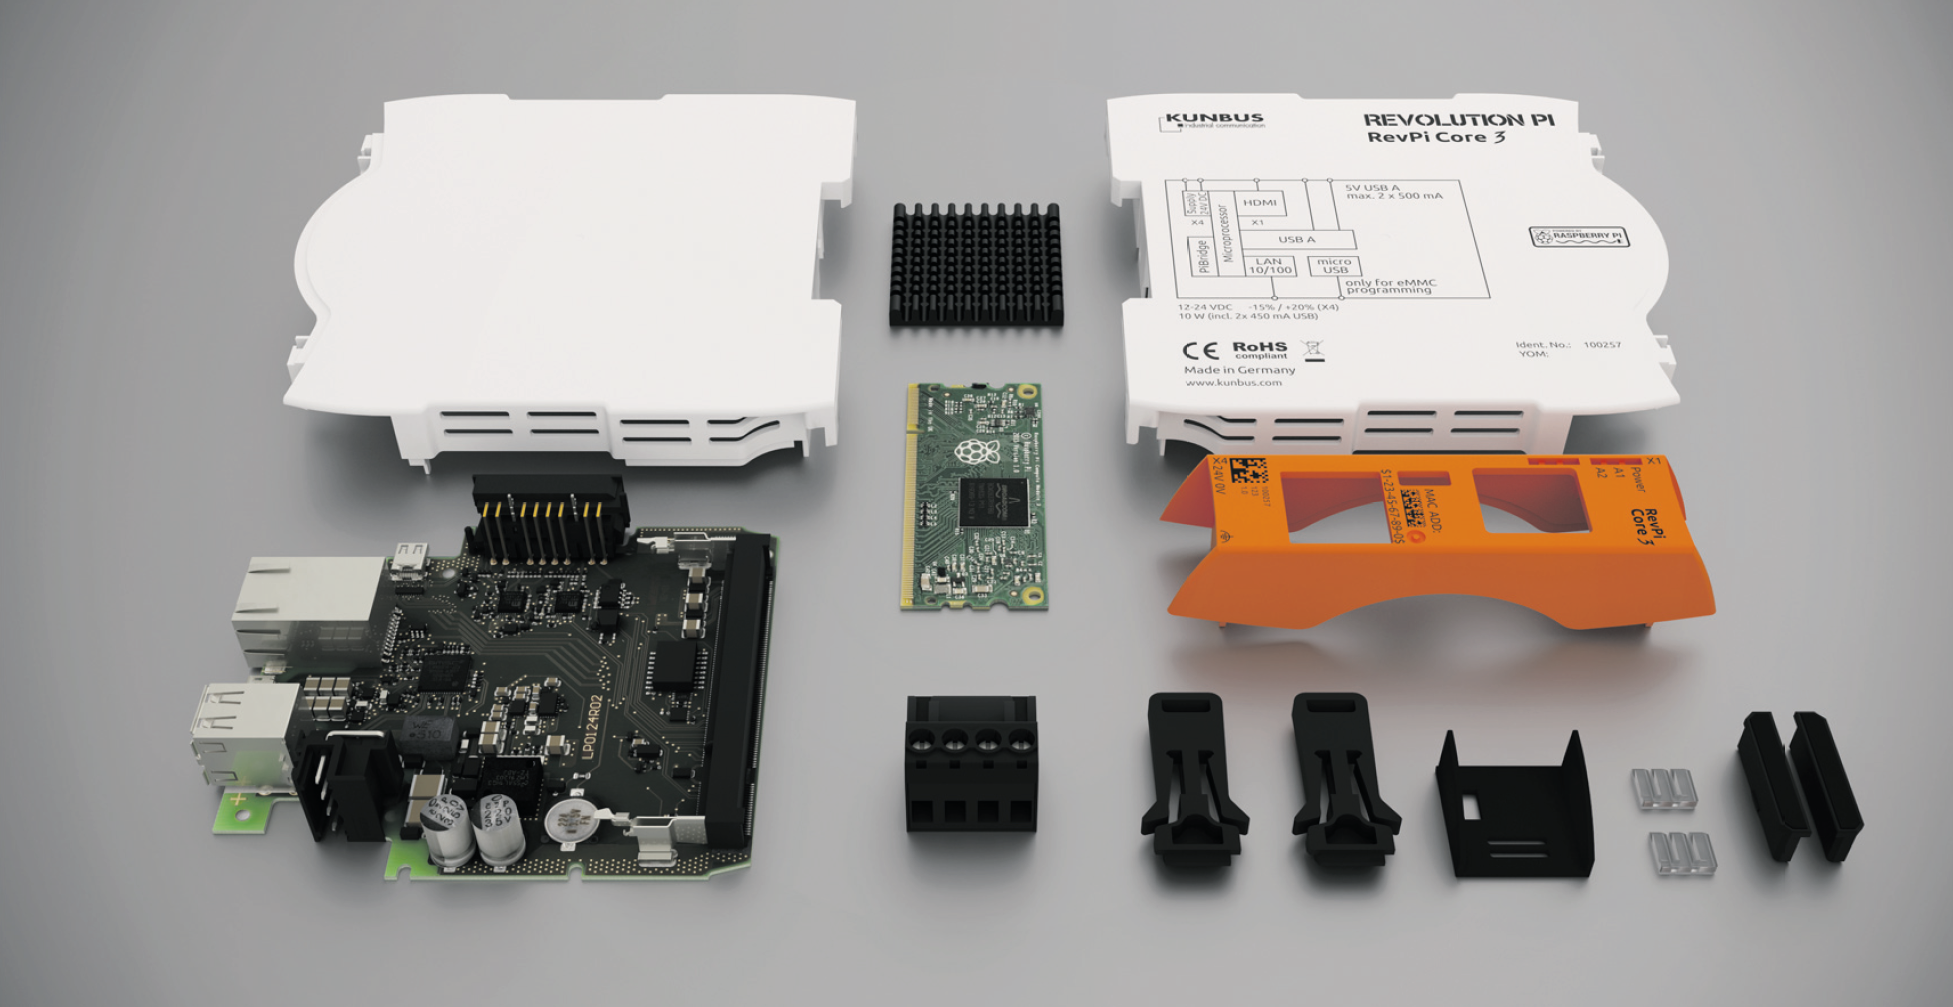
\includegraphics[width=0.85\textwidth]{doc/tex/images/revpi_teardown.png}
    \caption{Der RevPi Core 3 und seine Einzelkomponenten (Quelle: Kunbus)
      \label{fig:revpi-expl}}
\end{figure}

Spezifikationen des RevPi Core 3 \citep[Auswahl, vgl.][S. 1]{datasheet-revpi}:
\begin{itemize}
  \item{Prozessor: BCM2837}
  \item{Taktfrequenz 1,2 GHz}
  \item{Anzahl Prozessorkerne: 4}
  \item{Arbeitsspeicher: 1 GByte}
  \item{eMMC Flash Speicher: 4 GByte}
  \item{Betriebssystem: Angepasstes Raspbian mit RT-Patch}
  \item{RTC mit 24h Pufferung über wartungsfreien Kondensator}
  \item{Treiber / API: Kernel-Treiber schreibt zyklisch Prozessdaten in ein Prozessabbild, Zugriff auf Prozessabbild mittels ioctl-Anfragen oder über Linux-Dateisystem als API zu Fremdsoftware}
  \item{Kommunikationsanschlüsse: 2 x USB 2.0 A, 1 x Micro-USB, HDMI, Ethernet 10/100 Mbit/s}
  \item{Stromversorgung: min. 10,7 V, max. 28,8 V, maximal 10 Watt}
\end{itemize}

Kunbus stellt für den Revolution Pi ein auf Raspbian\footnote{Raspbian ist eine speziell 
für den Raspberry Pi angepasste Variante von Debian.} Stretch basierendes Betriebssystem bereit.
Verwendet wird der Kernel 4.9.76-rt60-v7+ in Verbindung mit dem SMP PREEMPT RT Patch.

\begin{figure}
    \centering
    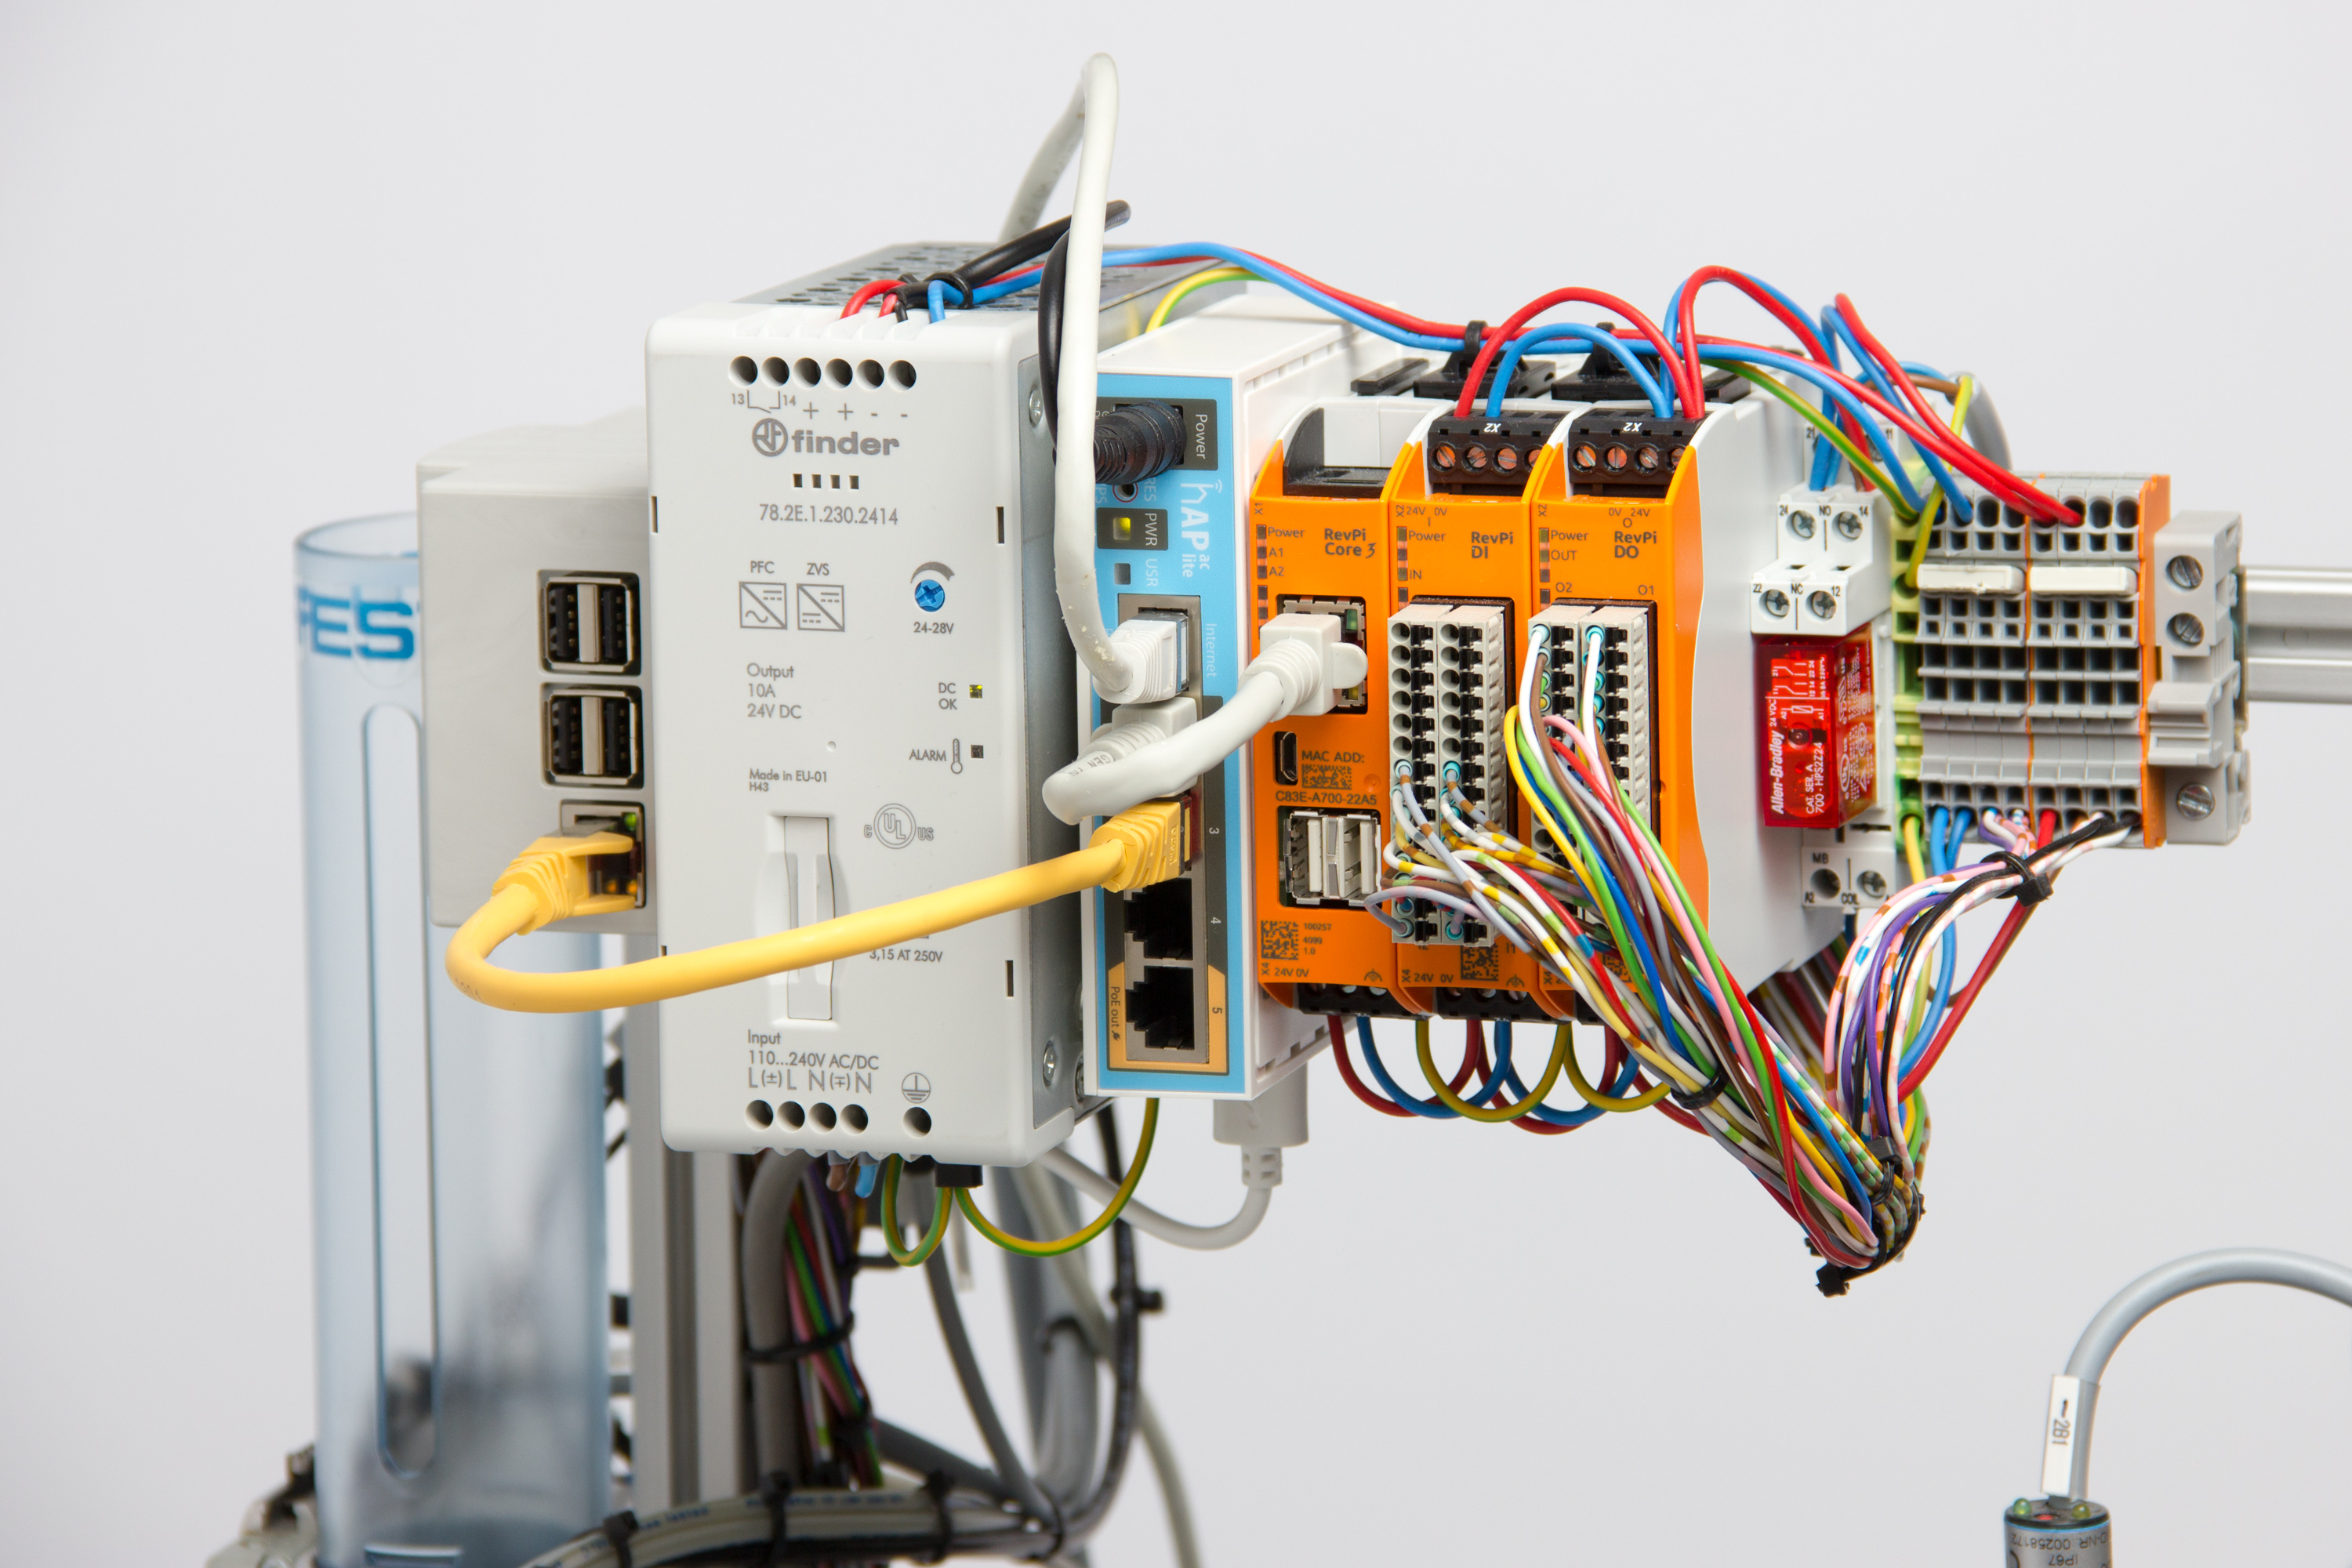
\includegraphics[trim={13cm 5cm 1cm 3cm}, clip, width=0.85\textwidth]{../photos/serverless_plc_img_8}
    \caption{Der Revolution Pi 3 mit digitalen IO-Modulen}
    \label{fig:rev-pi-io}
\end{figure}

Kunbus bietet neben dem sog. Core auch IO- und Gateway-Modulen zur Erweiterung der SPS an, siehe Bild~\ref{fig:rev-pi-io}.
Gateways dienen der Kommunikation mit externen Systemen oder Komponenten
über in der Automatisierungstechnik gängige Protokolle wie PROFIBUS oder EtherCAT. 
IO-Module erlauben die Überwachung und Steuerung von digitalen oder analogen Ein- und Ausgängen (IOs).

Kunbus deklariert die Hardware des Revolution Pi als Open-Source \citep[vgl.][S. 4]{flyer-revpi}. 
Die Schaltpläne des Revolution Pi, genauer die des RevPi Core 3 und der IO-Module, stehen auf der
Website\footnote{\label{downloads}\url{https://revolution.kunbus.com/tutorials/downloads/}} des Herstellers zum 
Download bereit. Eine Lizenz wird nicht angegeben.
Die Raspberry Pi Foundation stellt die Schaltpläne des Compute Modules des weiteren in ihrem Gitub-Repository 
zum Download bereit.

Sowohl die Raspberry Pi Foundation als auch die Kunbus GmbH pflegen aktiv ihre öffentlichen Repositories\footnote{\url{https://github.com/raspberrypi/} resp.~\url{https://github.com/RevolutionPi/}}
auf Github. 

% Kunbus konnte so einige Verbesserungen zum Linux Kernel 4.15 beitragen
% \footnote{siehe \url{https://revolution.kunbus.com/our-contribution-to-linux-4-15/}}.
% \todo{letzten Absatz evtl. weglassen? an sich nicht schlecht, passt aber irgendwie 
% nicht richtig zum Rest und stört den Lesefluss}

\subsubsection{Zugriff auf IO-Module%
        \label{sec:2-io}}
Der Zugriff auf die Ein- und Ausgänge der IO-Module erfolgt über einen RS485-Bus und einen in Form eines Kernel-Moduls bereitgestellten Treiber, genannt piControl. Der RS485-Bus ist über die serielle Schnittstelle des Compute Modules angebunden. 
piControl stellt ein Prozessabbild bereit, welches den physikalischen Zustand der Ein- und Ausgänge der IO-Module repräsentiert.
Das Prozessabbild wird, wie in der Automatisierungstechnik üblich, zyklisch aktualisiert. 
Die angestrebte Zykluszeit beträgt 5ms, kann jedoch je nach Anzahl der angeschlossenen Module auch größer sein. 
Kunbus garantiert bei drei IO-Modulen und zwei Gateway-Modulen eine Zykluszeit von 10 ms \citep[vgl.][]{web-revpi-dio}.
Die garantierte Zykluszeit ermöglicht die Umsetzung von Anwendungen mit harten Echtzeit-Anforderungen.

Fremdanwendungen können über eine Applikationsschnittstelle (API) auf das Prozessabbild zugreifen. 
Hierzu stellt das Kernel-Modul piControl sowohl \lstinline{seek}, \lstinline{read} und \lstinline{write} Methoden zur verfügung, wie auch die Möglichkeit mittels \lstinline{ioctl}-Anfragen gezielt auf einzelne Variablen des Prozessabbildes zuzugreifen.
In der englischsprachigen Wikipedia werden ioctl-Aufrufe wie folgt beschrieben:

\glqq{}The kernel is designed to be extensible, and may accept an extra module called a device driver which runs in kernel space and can directly address the device. An ioctl interface is a single system call by which userspace may communicate with device drivers. [...] The basic kernel can thus allow the userspace to access a device driver without knowing anything about the facilities supported by the device, and without needing an unmanageably large collection of system calls.

[...] ioctl calls provide a convenient way to bridge userspace code to kernel extensions. Kernel extensions can provide a location in the filesystem that can be opened by name, through which an arbitrary number of ioctl calls can be dispatched, allowing the extension to be programmed without adding system calls to the operating system.\grqq{}\citep[vgl.][]{web-wiki-ioctl}

Der Quellcode von piControl steht unter der GNU General Public License Version 2 (GNU GPLv2) und ist 
auf Github verfügbar\footnote{\url{https://github.com/RevolutionPi/piControl}}. Als Einstieg in die 
Entwicklung eigener Steuerungsprogramme liefert Kunbus das C-Programm piTest mit. Dieses verwendet 
piControl und erlaubt dem Nutzer über Kommandozeilen-Parameter die angeschlossenen IO-Module zu steuern.

\begin{figure}[h]
    \centering
    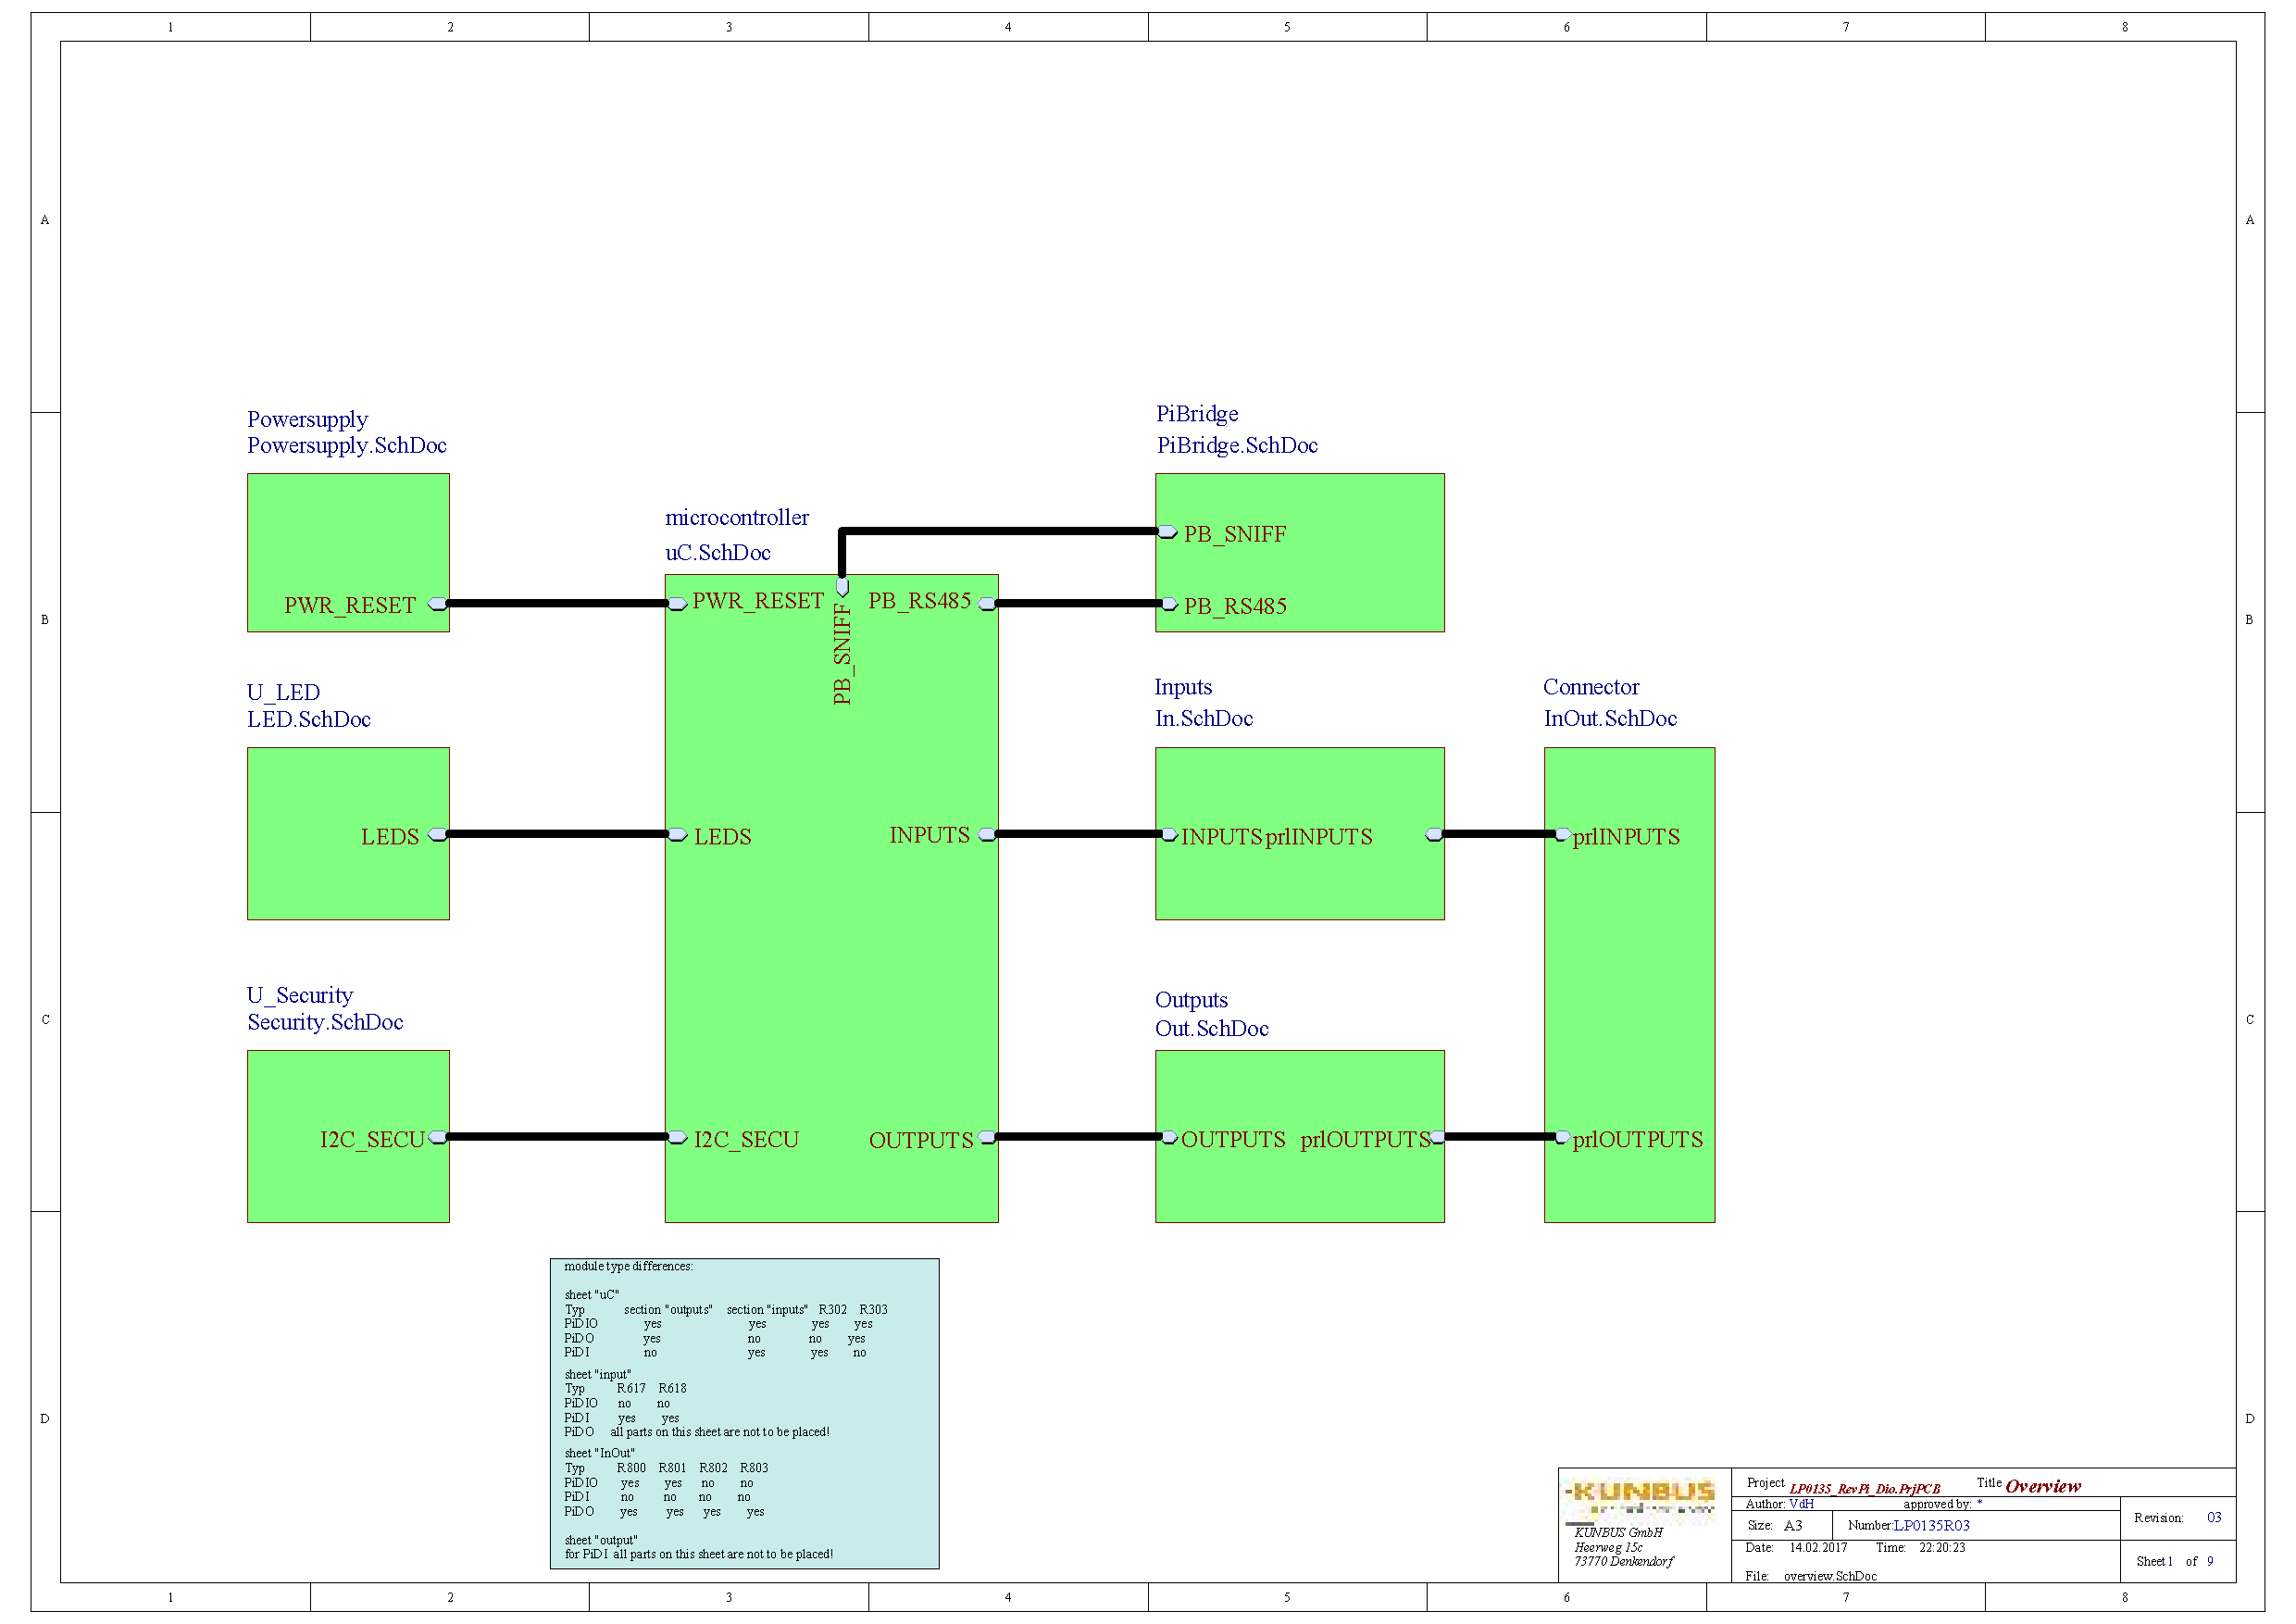
\includegraphics[trim={4cm 7cm 10.5cm 7.3cm}, clip, width=\textwidth]{literature/SchematicPrintsRevPi-DIO}
    \caption{Schematische Darstellung eines DIO-Moduls (Quelle: Kunbus\textsuperscript{\ref{downloads}})
      \label{fig:dio}}
\end{figure}

Jedes der IO-Module stellt ein eigenständiges eingebettetes System dar. Es verfügt
über einen Microcontroller, welcher die IOs bereitstellt und über einen RS485-Bus
mit dem Revolution Pi kommuniziert (siehe Bild~\ref{fig:dio}). 
Kunbus stellt exemplarisch den Quellcode eines DIO-Moduls unter der MIT Lizenz zur
Verfügung\footnote{\url{https://github.com/RevolutionPi/IODeviceExample}}. 


\subsection{Echtzeit und Multitasking unter Linux -- preemptRT und posix%
     \label{sec:2-echtzeit}}
     
Moderne Betriebssysteme realisieren Multitasking i.d.R.\,in Form des präemptiven Multitasking. 
Der Kernel verfügt über einen sog. Scheduler. Dieser priorisiert alle Prozesse und weist ihnen 
Rechenzeit in sog. Time Slots zu. Die Größe der Zeitfenster sowie die Ausführungsreihenfolge 
ist von der Priorität eines Prozesses abhängig. Besonders an einem präemptiven im Gegensatz zu einem kooperativen Scheduler ist dessen Fähigkeit, Tasks während ihrer Ausführung zu unterbrechen bzw. zu pausieren, wenn diese eine bestimmte Dauer überschreiten oder ein höher priorisierter Prozess (bspw. ausgelöst durch einen Interrupt oder durch eine inhärente Periodizität) Rechenleistung benötigt.

Eine Sonderform des präemptiven Multitasking ist das präemptible Multitasking. Hierbei werden auch Teile 
des Kernels als Threads durch den Scheduler ausgeführt. Dieser ist somit in der Lage, auch Prozesse des Kernels
zu unterbrechen, wenn andere Anwendungen Prozessorzeit oder Zugriff auf andere Systemressourcen benötigen
\citep[vgl.][]{web-wiki-praempt}.
     
Der Linux-Kernel implementiert unterschiedliche Präemptions-Modelle \citep[vgl.][/preemption\_models]{web-linuxwiki-basics}:

\begin{itemize}
  \item No Forced Preemption (server):
  Ausgelegt auf maximal möglichen Durchsatz, lediglich Interrupts und
  System-Call-Returns bewirken Präemption.

  \item Voluntary Kernel Preemption (Desktop):
  Neben den implizit bevorrechtigten Interrupts und System-Call-Returns gibt es
  in diesem Modell weitere Abschnitte des Kernels in welchen Preämption explizit
  gestattet ist.

  \item Preemptible Kernel (Low-Latency Desktop):
  In diesem Modell ist der gesamte Kernel, mit Ausnahme sog.~kritischer Abschnitte
  präemptible. Nach jedem kritischen Abschnitt gibt es einen impliziten Präemptions-Punkt.

  \item Preemptible Kernel (Basic RT):
  Dieses Modell ist dem zuvor genannten sehr ähnlich, hier sind jedoch alle Interrupt-Handler
  als eigenständige Threads ausgeführt.

  \item Fully Preemptible Kernel (RT):
  Wie auch bei den beiden zuvor genannten Modellen ist hier der gesamte Kernel
  präemtible. Die Anzahl und Dauer der nicht-präemtiblen kritischen Abschnitte
  ist auf ein notwendiges Minimum beschränkt. Alle Interrupt-Handler sind als
  eigenständige Threads ausgeführt, Spinlocks durch Sleeping-Spinlocks und Mutexe
  durch sog.~RT-Mutexe ersetzt.

\end{itemize}

Lediglich ein präemtibler Kernel kann hartes Echtzeit-Verhalten realisieren, 
da nur hier eine maximale Antwortzeit garantiert werden kann.
Viele Prozesse in der Automatisierungstechnik erfordern harte Echtzeit. 
Eine verspätete Antwort auf eine Anfrage, 
wie etwa das Signal eines Lagenendschalters oder eines Notausschalters kann hier nicht nur über
den Erfolg eines Prozesses, sondern auch über das Leben der daran beteiligten Mitarbeiter entscheiden.
Für weiterführende Erklärungen bzgl.\,Echtzeit, Mutexen und 
Spinlocks sei an dieser Stelle auf die Vorlesung verwiesen~\citep{script-peter}.


\subsubsection{preemptRT%
        \label{sec:2-preemptRT}}

Der Kernel des auf dem Revolution Pi installierten Raspbian mit PREEMP\_RT Patch fällt 
in die Kategorie des \glqq{}Fully Preemptible Kernels\grqq{} (siehe Abschnitt \ref{sec:2-echtzeit}).
Das zugrunde liegende Prinzip lässt sich wie folgt formulieren: Nur Code, welcher absolut nicht-präemtible sein darf, ist es
gestattet nicht-präemtible zu sein. Ziel ist folglich, die Menge des nicht-präemtiblen 
Codes im Linux-Kernel auf das absolut notwendige Minimum zu reduzieren.

Dies wird durch Verwendung folgender Mechanismen erreicht~\citep[vgl.][]{web-linuxwiki-details}:

\begin{itemize}
  \item Hochauflösende Timer
  \item Sleeping Spinlocks
  \item Threaded Interrupt Handlers
  \item rt\_mutex
  \item RCU
\end{itemize}

Diese Mechanismen sind bspw. im Linux-Wiki\footnote{siehe \url{https://wiki.linuxfoundation.org/realtime/documentation/technical_details}} ausführlich beschrieben.

\subsubsection{POSIX%
        \label{sec:2-posix}}
Das Portable Operating System Interface (POSIX) bezeichnet eine Sammlung von Standards, 
welche auf dem Unix-System basieren, jedoch nicht auf dieses beschränkt sind.

Der Wechsel zwischen verschiedenen Unix-Distributionen brachte oft Kompatibilitätsprobleme mit sich. 
Dieser Mangel an Portabilität erschwerte Benutzern und Entwicklern die Verwendung bzw. Bereitstellung 
von Software auf unterschiedlichen Systemen. 
Das Institut für Elektrotechnik und Elektronik (IEEE) begann 1984 mit der Entwicklung des Unix-Standards.
Sie entwickelten das, was heute als Single UNIX Specification bekannt ist und allgemein als POSIX bezeichnet wird~\citep[vgl.][]{web-debianwiki-posix}.
Das Konsortium \glqq{}The Open Group\grqq{} überwacht die weitere Entwicklung dieses Standards.
Ferner stellt es einen Teil der POSIX-Spezifikation frei zur Verfügung~\citep[vgl.][]{web-opengroup-posix}.

Die aktuelle Version POSIX.1-2017 ist verfügbar als IEEE Standard 1003.1-2017 sowie in Form der \glqq{}The Open Group Technical Standard Base Specifications\grqq{}, Ausgabe 7. POSIX.1-2017 definiert eine Standard-Betriebssystemschnittstelle und -umgebung, einschließlich eines Befehlsinterpreters (auch Shell genannt) und gängiger Dienstprogramme zur Unterstützung der Portabilität von Anwendungen auf Quellcode-Ebene. POSIX.1-2017 ist sowohl für Anwendungsentwickler als auch für Systemimplementierer gedacht und umfasst vier Hauptkomponenten \citep[vgl.][]{web-opengroup-overview}:
\begin{itemize}
    \item Basisdefinitionen:\\
          Allgemeine Begriffe, Konzepte und Schnittstellen einschließlich Hilfskonventionen und C-Headern
          
    \item Systemschnittstellen:\\
          Definitionen für Systemdienstfunktionen und Unterprogramme, C-spezifische Systemdienste, Portabilität
        
    \item Shell und Dienstprogramme:\\
          Definitionen für eine Schnittstelle zur Befehlsinterpretation von Diensten und gängige Hilfsprogramme
    
    \item Begründungen und Historie
\end{itemize}

Debian basiert auf Linux und verwendet den Linux-Kernel. Linux ist zu großen Teilen POSIX-kompatibel. Debian ist jedoch nicht POSIX-zertifiziert, da diese Zertifizierung mit hohen Kosten verbunden ist\citep[vgl.][Kapitel 4.4.]{web-debian-faq}.

Beide Kernkomponenten des in dieser Arbeit vorgestellten Projektes nutzen Komponenten von Linux, 
welche an den POSIX-Standard angelehnt sind: open62541 verwendet u.a.\,POSIX-Threads und
Mutexe~\citep[vgl.][pthread.h]{web-opengroup-pthread}, piControl nutzt POSIX-Semaphoren
\citep[vgl.][semaphore.h]{web-opengroup-semaphore}. 


\subsection{OPC-UA und open62541%
     \label{sec:2-opc}}
In diesem Abschnitt sollen Möglichkeiten des Datenaustausch zwischen Komponenten der
Automatisierungstechnik vorgestellt werden. OPC-UA stellt einen offenen, IP-basierten Kommunikationsstandard
für Sensoren und Steuerungen dar. open62541 ist eine freie Client- sowie Server-Implementierung dieses
Standards, geschrieben in C.


\subsubsection{OPC UA%
        \label{sec:2-opcua}}

Open Platform Communications (OPC) ist eine Familie von Standards zur herstellerunabhängigen
Kommunikation von Maschinen (M2M) in der Automatisierungstechnik. Die sog. OPC Task Force, zu deren
Mitgliedern verschiedene etablierte Firmen der Automatisierungsindustrie gehören, veröffentlichte
die OPC Specification Version 1.0 im August 1996.
Motiviert ist dieser offene Standard durch die Erkenntniss, dass die Anpassung der
zahlreichen Herstellerstandards an individuelle Infrastrukturen und Anlagen einen
großen Mehraufwand verursachen.
Die Wikipedia beschreibt das Anwendungsgebiet für OPC wie folgt \citep[vgl.][]{web-wiki-opc}:

\glqq{}OPC wird dort eingesetzt, wo Sensoren, Regler und Steuerungen verschiedener Hersteller
ein gemeinsames Netzwerk bilden. Ohne OPC benötigten zwei Geräte zum Datenaustausch
genaue Kenntnis über die Kommunikationsmöglichkeiten des Gegenübers. Erweiterungen
und Austausch gestalten sich entsprechend schwierig. Mit OPC genügt es, für jedes
Gerät genau einmal einen OPC-konformen Treiber zu schreiben. Idealerweise wird
dieser bereits vom Hersteller zur Verfügung gestellt. Ein OPC-Treiber lässt sich
ohne großen Anpassungsaufwand in beliebig große Steuer- und Überwachungssysteme
integrieren.

OPC unterteilt sich in verschiedene Unterstandards, die für den jeweiligen Anwendungsfall
unabhängig voneinander implementiert werden können. OPC lässt sich damit verwenden
für Echtzeitdaten (Überwachung), Datenarchivierung, Alarm-Meldungen und neuerdings
auch direkt zur Steuerung (Befehlsübermittlung).\grqq{}

OPC basiert in der ursprünglichen Spezifikation (auch als OPC DA bezeichnet) auf Microsofts DCOM-Spezifikation.
DCOM macht Funktionen und Objekte einer Anwendung anderen Anwendungen im Netzwerk
zugänglich. Der OPC-Standard definiert entsprechende DCOM-Objekte um mit anderen
OPC-Anwendungen Daten austauschen zu können. Die Verwendung von DCOM bindet Anwender
jedoch an Betriebssysteme von Microsoft. 

\begin{figure}
    \centering
    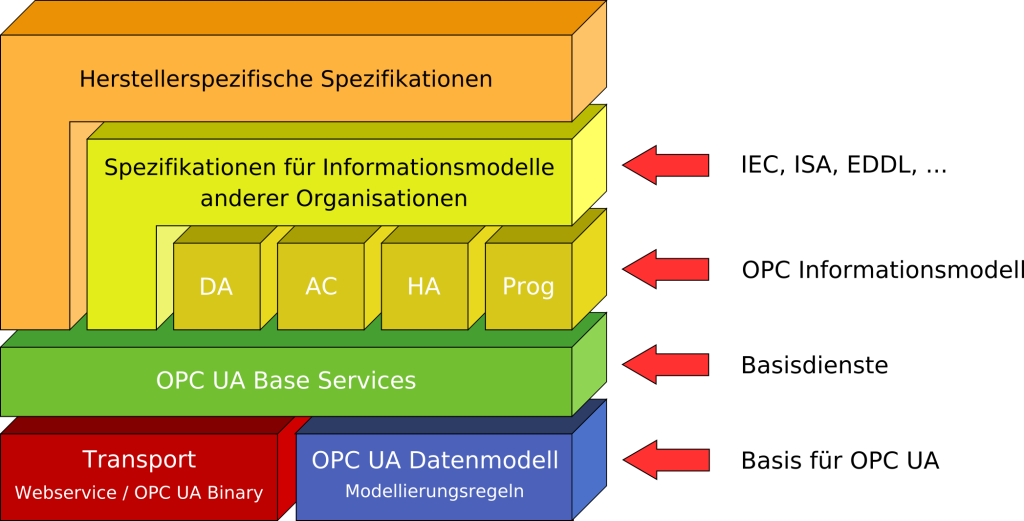
\includegraphics[width=0.85\textwidth]{images/UA_Architecture_1024.png}
    \caption{Die OPC Unified Architecture. Grafik von Gerhard Gappmeier - ascolab GmbH, CC BY-SA 3.0}
    \label{fig:opc-unified-architecture}
\end{figure}
% Evtl Grafik: Von Gerhard Gappmeier - ascolab GmbH, CC BY-SA 3.0, https://de.wikipedia.org/w/index.php?curid=1892069

Die ursprüngliche OPC Spezifikation wurde 2006 durch die Entwicklung der 
OPC Unified Architecture (OPC UA) überholt. 
Diese zeichnet sich durch eine Service-orientierte Architektur (SOA) aus, deren Struktur
aus mehreren Schichten besteht, siehe Abbilung~\ref{fig:opc-unified-architecture}. 
Über der untersten Schicht, dem Betriebssystem des Servers, verbindet eine Portabilitäts-Schicht 
den sog.\, UA ANSI C Stack mit einer API. Diese API kann bspw.\,in C++ geschrieben sein, 
und erlaubt die Anbindung der obersten Schicht, der Anwendungsschicht~\citep[vgl.][]{web-spec-opc}.
OPC UA setzt auf einem eigenen Kommunikationsstack auf; die Verwendung von DCOM
und damit die Bindung an Microsoft wurden aufgelöst.

Neben Architektur und Kommunikationsschnittstellen wird in der OPC Spezifikation auch ein 
Informationsmodell definiert. Die deutschsprachige Wikipedia beschreibt dieses wie folgt: 

\glqq{}Das OPC[-UA]-Informationsmodell ist nicht mehr nur eine Hierarchie aus Ordnern, Items
und Properties. Es ist ein sogenanntes Full-Mesh-Network aus Nodes, mit dem neben
den Nutzdaten eines Nodes auch Meta- und Diagnoseinformationen repräsentiert werden. [...]
Ein Node ähnelt einem Objekt aus der objektorientierten Programmierung. Ein Node
kann Attribute besitzen, die gelesen werden können. Es ist möglich Methoden zu definieren und aufzurufen. [...]
Weiterhin werden Events unterstützt, die versendet werden können
(AE (Alarms \& Events), DA DataChange), um bestimmte Informationen zwischen Geräten
auszutauschen. Ein Event besitzt unter anderem einen Empfangszeitpunkt, eine Nachricht
und einen Schweregrad. Die o.\,g. Nodes werden sowohl für die Nutzdaten als auch
alle anderen Arten von Metadaten verwendet. Der damit modellierte OPC-Adressraum
beinhaltet nun auch ein Typmodell, mit dem sämtliche Datentypen spezifiziert werden.\grqq{}


\subsubsection{open62541%
        \label{sec:2-open62541}}
open62541 ist eine offene und freie Implementierung von OPC UA. 
Die in C geschriebene Bibliothek stellt eine beständig zunehmende Anzahl der im OPC UA Standard definierten
Funktionen bereit. Sie kann sowohl zur Erstellung von OPC-Servern als auch von -Clients
genutzt werden. Ergänzend zu der unter der Mozilla Public License v2.0 lizensierten
Bibliothek stellt das open62541 Projekt auch Beispielprogramme unter einer CC0 Lizenz
zur Verfügung.
Zu den Unterstützern des Projektes zählen u.a.\, die RWTH Aachen, das Frauenhofer IOSB sowie die TU Dresden.

Die Bibliothek eignet sich auch für die Entwicklung auf eingebetteten Systemen und
Microcontrollern. Die Größe einer Server-Binary kann weniger als 100kB betragen.

Folgende Auswahl an Eigenschaften und Funktionen zeichnet die in dieser Arbeit verwendete
Version 0.3 von open62541 aus:
\begin{itemize}
  \item Kommunikationionsstack
  \begin{itemize}
      \item OPC UA Binär-Protokoll (HTTP oder SOAP werden gegenwärtig nicht unterstützt)
      \item Austauschbare Netzwerk-Schicht, welche die Verwendung eigener Netzwerk-APIs
      erlaubt.
      \item Verschlüsselte Kommunikationion
      \item Asynchrone Dienst-Anfragen im Client
  \end{itemize}
  \item Informationsmodell
  \begin{itemize}
    \item Unterstützung aller OPC UA Node-Typen, inkl.~Methoden
    \item Hinzufügen und Entfernen von Nodes und Referenzen zur Laufzeit.
    \item Vererbung und Instanziierung von Objekt- und Variablentypen
    \item Zugriffskontrolle auch für einzelne Nodes
  \end{itemize}
  \item Subscriptions
  \begin{itemize}
    \item Erlaubt die Überwachung (subscriptions / monitoreditems)
    \item Sehr geringer Ressourcenbedarf pro überwachtem Wert
  \end{itemize}
  \item Code-Generierung auf XML-Basis
  \begin{itemize}
    \item Erlaubt die Erstellung von Datentypen
    \item Erlaubt die Generierung des serverseitigen Informationsmodells
  \end{itemize}
\end{itemize}

Weiterführende Informationen und Code-Beispiele bietet die ausführliche Dokumentation des Projektes~\citep[siehe]{web-open62541} sowie der kommentierte Quelltext.

% % % Imports nur für Referenzenauflösung während des Schreibens! Vorm Kompilieren auskommentieren!
% \bibliography{0_hauptdatei}
% \input{1_einleitung}
% \input{2_grundlagen}
% \input{3_konzeption}
% \input{4_implementierung}
% \input{5_tests}
% \input{6_zusammenfassung}
% \input{anhang}
% % Ende Imports

\section{Systemkonzept%
  \label{sec:3-konzeption}}
Auf Basis der in Abschnitt [...] vorgestellten Möglichkeiten folgt nun die Ausarbeitung eines Konzepts.

\subsection{Anbindung der IO an den OPC-Server%
     \label{sec:3-anbindung}}

\subsection{Integration des OPC-Servers in das System%
     \label{sec:3-integration}}

% % % Imports nur für Referenzenauflösung während des Schreibens! Vorm Kompilieren auskommentieren!
% \bibliography{0_hauptdatei}
% \input{1_einleitung}
% \input{2_grundlagen}
% \input{3_konzeption}
% \input{4_implementierung}
% \input{5_tests}
% \input{6_zusammenfassung}
% \input{anhang}
% % Ende Imports

\section{Implementierung%
  \label{sec:4-implementierung}}
Das folgende Kapitel stellt in Auszügen die Implementierung des OPC-Servers sowie die Anbindung an die IO-Module
der SPS dar. Der Schwerpunkt liegt hierbei auf der Funktionsweise des piControl-Treibers und dessen Integration in das Projekt. Abschnitt~\ref{sec:4-picontrol} erklärt die zum Schreibens eines Bits verwendeten Funktionsaufrufe.
Zuvor soll jedoch in Abschnitt~\ref{sec:4-open62541} der Teil des OPC-Servers vorgestellt werden, welcher auf besagten Treiber zugreift. 

\subsection{Implementierung des OPC-Servers%
     \label{sec:4-open62541}}
Wie im vorangegangenen Abschnitt~\ref{sec:3-integration} begründet, soll die Verknüpfung zwischen dem Prozessabbild der SPS und den auf dem OPC-Server bereitgestellten Werten über sog.\,Datenquellen erfolgen. Hierzu ist zunächst eine Callback-Methode zu implementieren, welche bei einem Lese- oder Schreibzugriff auf eine Variable aufgerufen wird. Die Verknüpfung zwischen Callback-Methode und Variable muss manuell erfolgen.

\begin{lstlisting}[language={c},firstnumber=237,caption={Auszug der Methode \lstinline{linkDataSourceVariable} in \lstinline{variables.c}\label{lst:4-linkDataSourceVariable}}]
extern UA_StatusCode
 linkDataSourceVariable(UA_Server *server, UA_NodeId nodeId) {
     bool readonly = false;
     UA_DataSource dataSourceVariable;
     UA_StatusCode rc; |>\setcounter{lstnumber}{254}<|

     dataSourceVariable.read = readDataSourceVariable;
     if (!readonly)
        dataSourceVariable.write = writeDataSourceVariable;
     else
        dataSourceVariable.write = writeReadonlyDataSourceVariable;

     return UA_Server_setVariableNode_dataSource(server, nodeId, dataSourceVariable);
 }
\end{lstlisting}

\begin{figure}[h]
    \centering
    \includegraphics[width=0.42\textwidth]{doc/img/OPC_RevPiDO.pdf}
    \caption{Auszug des verwendeten Nodesets, hier Digitalausgang 1 des Versuchsaufbaus
      \label{fig:opc-do}}
\end{figure}

Die in Listing~\ref{lst:4-linkDataSourceVariable} abgebildete Methode \lstinline{linkDataSourceVariable()} erzeugt ein Struct vom Typ \lstinline{UA_DataSource}. In diesem werden dem Lesen und Schreiben einer OPC-Variablen entsprechende Callback-Methoden zugewiesen. Die Verknüpfung einer OPC-Variable, genauer ihrer NodeId, mit der zuvor definierten Datenquelle erfolgt über die von open62541 bereitgestellte Methode \lstinline{UA_Server_setVariableNode_dataSource()}. Vor dem Lesen und nach dem Schreiben dieser Variable werden von nun an die entsprechenden Callbacks aufgerufen.
     
\begin{lstlisting}[language={c},firstnumber=168,caption={Auszug des Callbacks \lstinline{writeDataSourceVariable} in \lstinline{variables.c}\label{lst:4-writeDataSourceVariable}}]  
extern UA_StatusCode
 writeDataSourceVariable(UA_Server *server,
            const UA_NodeId *sessionId, void *sessionContext,
            const UA_NodeId *nodeId, void *nodeContext,
            const UA_NumericRange *range, const UA_DataValue *dataValue) {

    UA_StatusCode retval  = UA_STATUSCODE_GOOD;
    UA_NodeId *nameNodeId = UA_malloc(sizeof(UA_NodeId));
    UA_QualifiedName nameQN = UA_QUALIFIEDNAME(1, "Name");
    UA_Variant nameVar;
    UA_Boolean bit;

    retval |= findSiblingByBrowsename(server, nodeId, &nameQN, nameNodeId);
    retval |= UA_Server_readValue(server, *nameNodeId, &nameVar);
    retval |= UA_Boolean_copy(dataValue->value.data, &bit);

    |>\tikzmarkin[set border color=martinired]{writeIO}<|PI_writeSingleIO(String_fromUA_String(nameVar.data), &bit, false);                                                 |>\tikzmarkend{writeIO}<|

    free(nameNodeId);
    return retval;
 }
\end{lstlisting}

Listing~\ref{lst:4-writeDataSourceVariable} zeigt die Callback-Methode, welche nach dem Schreiben einer Variablen auf dem OPC-Server aufgerufen wird.
Dieser Methode wird neben der NodeId der mit ihr verknüpften Variablen auch der Wert dieser in Form eines Zeigers auf ein Struct vom Typ \lstinline{UA_DataValue} übergeben.

Die Gestaltung des hier verwendeten Nodesets sieht vor, dass in einer OPC-Variablen \lstinline{"Name"} der Bezeichner des zu schreibenden Digitalausgangs hinterlegt ist, siehe Abbildung~\ref{fig:opc-do}. Dies erlaubt eine Rekonfiguration der Ein- und Ausgänge der SPS ohne Änderungen im Programmcode des OPC-Servers vornehmen zu müssen.
Es ist daher erforderlich, nach jedem Schreiben einer mit einem Digitalausgang verknüpften Variablen, hier \lstinline{"Value"}, dessen Bezeichner \lstinline{"Name"} abzufragen. 
Dies geschieht in den Zeilen 180 und 181.
Anschließend wird dieser Bezeichner sowie der zu schreibende Wert der Methode \lstinline{PI_writeSingleIO()} übergeben, welche wiederum die Interaktion mit piControl übernimmt (vgl. Abschnitt \ref{sec:4-picontrol}).
 
\subsection{Integration von piControl%
     \label{sec:4-picontrol}}
In Abschnitt~\ref{sec:2-io} wurde die Anbindung der IO-Module des Revolution Pi sowie die Funktionsweise von piControl aus Anwendersicht beschrieben. Die verfügbare Literatur beschränkt sich auch auf lediglich diese Sicht; eine weiterführende Dokumentation für Entwickler gibt es, neben der in Abschnitt~\ref{sec:3-anbindung} vorgestellten Manpage, nicht. 
In diesem Abschnitt soll daher der Quellcode von piControl sowie dessen Verwendung im Projekt genauer betrachtet werden.
Hierzu wird exemplarisch die in Abschnitt~\ref{sec:4-open62541} eingeführte Methode \lstinline{PI_writeSingleIO()} untersucht.
Diese Methode ermöglicht das Setzen eines einzelnen Bits im Prozessabbild der SPS, und damit das Schalten eines digitalen Ausgangs auf einem IO-Modul.
Die äquivalente Methode \lstinline{int piControlGetBitValue(SPIValue *pSpiValue)} zum Lesen eines Bits bzw. Eingangs funktioniert analog und soll daher an dieser Stelle nicht dediziert erörtert werden.

\begin{lstlisting}[language={c},firstnumber=97,
                   caption={Setzen eines phsikalischen, digitalen Ausgangs in \lstinline{revpi.c}
                   \label{lst:4-PI_writeSingleIO}}]
extern void PI_writeSingleIO(char *pszVariableName, bool *bit, bool verbose)
{
	int rc;
	SPIVariable sPiVariable;
	SPIValue sPIValue;

	strncpy(sPiVariable.strVarName, pszVariableName, sizeof(sPiVariable.strVarName));
	rc = piControlGetVariableInfo(&sPiVariable);
	if (rc < 0) {
		printf("Cannot find variable '%s'\n", pszVariableName);
		return;
	}

		sPIValue.i16uAddress = sPiVariable.i16uAddress;
		sPIValue.i8uBit = sPiVariable.i8uBit;
		sPIValue.i8uValue = *bit;
		rc = |>\tikzmarkin[set border color=martinired]{setBitValue}<|piControlSetBitValue(&sPIValue)|>\tikzmarkend{setBitValue}<|;
		if (rc < 0)
			printf("Set bit error %s\n", getWriteError(rc));
		else if (verbose)
			printf("Set bit %d on byte at offset %d. Value %d\n", sPIValue.i8uBit, sPIValue.i16uAddress,
			       sPIValue.i8uValue);
}
\end{lstlisting}

Der Programmcode in Listing~\ref{lst:4-PI_writeSingleIO} ist Teil des implementierten OPC-Servers. In diesem wird auf zwei Funktionen des piControl-Treibers zugegriffen. 
Beiden Methoden wird als Argument ein Zeiger auf ein Struct vom Typ \lstinline{SPIValue} übergeben. Der im Struct abgelegte Name wird mittels \lstinline{piControlGetVariableInfo(&sPIValue)} zu einer Adresse im Prozessabbild aufgelöst. Diese wird in \lstinline{sPIValue.i16uAdress} gespeichert. Der Wert der Variablen wird anschließend mittels \lstinline{piControlSetBitValue(&sPIValue)} an dieser Adresse in das Prozessabbild geschrieben.

\begin{lstlisting}[language={c},firstnumber=309,caption={Methode \lstinline{piControlSetBitValue} in \lstinline{piControlIf.c}\label{lst:4-piControlSetBitValue}}]
int |>\tikzmarkin[set border color=martiniblue]{setBitValueFcn}<|piControlSetBitValue(SPIValue *pSpiValue)|>\tikzmarkend{setBitValueFcn}<|
{
    piControlOpen();

    if (PiControlHandle_g < 0)
	    return -ENODEV;

    pSpiValue->i16uAddress += pSpiValue->i8uBit / 8;
    pSpiValue->i8uBit %= 8;

    if (|>\tikzmarkin[set border color=martinired]{ioctl}<|ioctl(PiControlHandle_g, KB_SET_VALUE, pSpiValue)|>\tikzmarkend{ioctl}<| < 0)
	    return errno;

    return 0;
}
\end{lstlisting}

Die in Listing~\ref{lst:4-piControlSetBitValue} dargestellte Methode \lstinline{piControlSetBitValue} ist lediglich eine Hüllfunktion (häufig auch als Wrapper-Funktion bezeichnet) für einen Aufruf des \lstinline{ioctl} Kernel-Moduls.
Folgende Parameter werden übergeben:
\lstinline{PiControlHandle_g} ist die Referenz auf die Geräte-Datei des piControl-Treibers. \lstinline{KB_SET_VALUE} ist das ioctl-Kommando zum Schreiben eines Bits in das Prozessabbild. Der Zeiger \lstinline{pSpiValue} verweist auf ein Struct des bereits vorgestellten Typs \lstinline{SPIValue}.

\begin{lstlisting}[language={c},firstnumber=80,caption={Methode \lstinline{piControlOpen} in \lstinline{piControlIf.c}\label{lst:4-piControlOpen}}]
void piControlOpen(void)
{
    /* open handle if needed */
    if (PiControlHandle_g < 0)
    {
	    |>\tikzmarkin[set border color=martiniblue]{PiControlHandle}<|PiControlHandle_g = open(PICONTROL_DEVICE, O_RDWR)|>\tikzmarkend{PiControlHandle}<|;
    }
}
\end{lstlisting}

Die in Listing~\ref{lst:4-piControlOpen} dargestellte Methode öffnet, sofern nicht bereits geschehen, die Geräte-Datei. Das Macro \lstinline{PICONTROL_DEVICE} verweist hierbei auf \lstinline{/dev/piControl0}.

\begin{lstlisting}[language={c},firstnumber=721,caption={Methode \lstinline{piControlIoctl} in \lstinline{piControlMain.c}\label{lst:4-piControlIoctl}}]
static long |>\tikzmarkin[set border color=martiniblue, below offset=0.9em]{piControlIoctl}<|piControlIoctl(struct file *file, unsigned int prg_nr, 
                           unsigned long usr_addr)                                      |>\tikzmarkend{piControlIoctl}<|
{
  int status = -EFAULT;
  tpiControlInst *priv;
  int timeout = 10000;	// ms

  if (prg_nr != KB_CONFIG_SEND && prg_nr != KB_CONFIG_START && !isRunning()) {
  	return -EAGAIN;
  }

  priv = (tpiControlInst *) file->private_data;

  if (prg_nr != KB_GET_LAST_MESSAGE) {
  	// clear old message
  	priv->pcErrorMessage[0] = 0;
  }

  switch (prg_nr) {|>\setcounter{lstnumber}{864}<|

    case |>\tikzmarkin[set border color=martiniblue]{KB_SET_VALUE}<|KB_SET_VALUE:|>\tikzmarkend{KB_SET_VALUE}<|
  		{
  			SPIValue *pValue = (SPIValue *) usr_addr;

  			if (!isRunning())
  				return -EFAULT;

  			if (pValue->i16uAddress >= KB_PI_LEN) {
  				status = -EFAULT;
  			} else {
  				INT8U i8uValue_l;
  				my_rt_mutex_lock(&piDev_g.lockPI);
  				i8uValue_l = piDev_g.ai8uPI[pValue->i16uAddress];

  				if (pValue->i8uBit >= 8) {
  					i8uValue_l = pValue->i8uValue;
  				} else {
  					if (pValue->i8uValue)
  						i8uValue_l |= (1 << pValue->i8uBit);
  					else
  						i8uValue_l &= ~(1 << pValue->i8uBit);
  				}

  				|>\tikzmarkin[set border color=martinired]{i8uValue}<|piDev_g.ai8uPI[pValue->i16uAddress] = i8uValue_l;|>\tikzmarkend{i8uValue}<|
  				rt_mutex_unlock(&piDev_g.lockPI);

  #ifdef VERBOSE
  				pr_info("piControlIoctl Addr=%u, bit=%u: %02x %02x\n", pValue->i16uAddress, pValue->i8uBit, pValue->i8uValue, i8uValue_l);
  #endif

  				status = 0;
  			}
  		}
  		break; |>\setcounter{lstnumber}{1314}<|

    default:
      pr_err("Invalid Ioctl");
      return (-EINVAL);
      break;

    }

    return status;
  }
\end{lstlisting}

Listing~\ref{lst:4-piControlIoctl} zeigt in Auszügen die ioctl-Methode des piControl Kernel-Treibers. Diese bekommt folgende Argumente übergeben: \lstinline{struct file *file} enthält den Verweis auf die Geräte-Datei, hier \lstinline{/dev/piControl0}. Der Wert von \lstinline{unsigned int prg_nr} beschreibt die Anfrage an den Treiber, in diesem Fall \lstinline{KB_SET_VALUE}. Das Argument \lstinline{unsigned long usr_addr} enthält einen typ-agnostischen Pointer. Dieser verweist auf einen Speicherbereich, in welchem die zur Bearbeitung der Anfrage notwendigen Daten abgelegt sind. Hier können auch vom Treiber empfangene Daten dem Anwendungsprogramm bereitgestellt werden. 

Die switch-case-Anweisung führt die über das Argument \lstinline{prg_nr} spezifizierte Aktion aus. Hier betrachten wir \lstinline{KB_SET_VALUE}:
Zunächst wird in Zeile 868 der übergebene Zeiger \lstinline{usr_addr} mittels explizitem Typecast zu einem Zeiger des Typs \lstinline{SPIValue *} konvertiert. Da dieser auf Daten im Userspace verweist, ist beim Zugriff durch den Kernel-Treiber besondere Vorsicht geboten.
In Zeile 877 wird mittels Mutex das Prozessabbild \lstinline{piDev_g} für den Zugriff durch andere Threads oder Prozesse gesperrt.
\lstinline{my_rt_mutex_lock} verweist hierbei auf die Funktion \lstinline{rt_mutex_lock} aus \lstinline{linux/sched.h}\footnote{Offenbar wurde hier auch eine alternative Implementierung vorgesehen, siehe revpi\_common.h}

In Zeile 889 wird das Byte \lstinline{i8uValue_l}, welches den zu schreibenden Wert enthält in das Prozessabbild übertragen. Anschließend wird die Mutex auf \lstinline{piDev_g} wieder entsperrt.
\newpage

\begin{lstlisting}[language={c},firstnumber=62,caption={Auszug des Struct \lstinline{spiControlDev} in \lstinline{piControlMain.h}\label{lst:4-spiControlDev}}]
|>\tikzmarkin[set border color=martiniblue]{spiControlDev}<|typedef struct spiControlDev|>\tikzmarkend{spiControlDev}<| {
	// device driver stuff
	int init_step;
	enum revpi_machine machine_type;
	void *machine;
	struct cdev cdev;	// Char device structure
	struct device *dev;
	struct thermal_zone_device *thermal_zone;

	|>\tikzmarkin[set border color=martiniblue]{processImage}<|// process image stuff
	INT8U ai8uPI[KB_PI_LEN];
	INT8U ai8uPIDefault|>\tikzmarkin[set border color=martinired]{KB_PI_LEN_0}<|[KB_PI_LEN]|>\tikzmarkend{KB_PI_LEN_0}<|;
	struct rt_mutex lockPI;        |>\tikzmarkend{processImage}<|
	bool stopIO;
	piDevices *devs; |>\setcounter{lstnumber}{94}<|
} tpiControlDev;
\end{lstlisting}

Das Prozessabbild ist als Byte-Array der Länge \lstinline{KB_PI_LEN} in Listing~\ref{lst:4-spiControlDev} definiert. Konfigurationsparameter wie \lstinline{KB_PI_LEN} oder die Zykluszeit für den Datenaustausch zwischen SPS und IO-Modulen sind im folgenden Listing~\ref{lst:4-process} definiert.

\begin{lstlisting}[language={c},firstnumber=119,caption={Konfigurationsparameter des Prozessabbildes in project.h\label{lst:4-process}}]
#define INTERVAL_PI_GATE (5*1000*1000)  // 5 ms piGateCommunication |>\setcounter{lstnumber}{128}<|

#define INTERVAL_IO_COM (5*1000*1000)  // 5 ms piIoComm |>\setcounter{lstnumber}{132}<|

#define KB_PD_LEN       512
|>\tikzmarkin[set border color=martiniblue]{KB_PI_LEN_1}<|#define KB_PI_LEN       4096|>\tikzmarkend{KB_PI_LEN_1}<|
\end{lstlisting}

Das zu setzende Bit wurde zu diesem Zeitpunkt erfolgreich in das Prozessabbild der SPS geschrieben.
Es stellt sich die Frage, wie dieses nun an das IO-Modul kommuniziert wird.
Die Kommunikation mit allen angebundenen Modulen ist ebenfalls Aufgabe des piControl-Treibers.

\begin{lstlisting}[language={c},firstnumber=256,caption={Auszug der Methode \lstinline{piIoThread} in \lstinline{revpi_core.c}\label{lst:4-piIoThread}}]
static int piIoThread(void *data)
{
	//TODO int value = 0;
	ktime_t time;
	ktime_t now;
	s64 tDiff;

	hrtimer_init(&piCore_g.ioTimer, CLOCK_MONOTONIC, HRTIMER_MODE_ABS);
	piCore_g.ioTimer.function = piIoTimer;

	pr_info("piIO thread started\n");

	now = hrtimer_cb_get_time(&piCore_g.ioTimer);

	PiBridgeMaster_Reset();

	while (!kthread_should_stop()) {
		if (|>\tikzmarkin[set border color=martinired]{PiBridgeMaster}<|PiBridgeMaster_Run()|>\tikzmarkend{PiBridgeMaster}<| < 0)
			break;
	}

	RevPiDevice_finish();

	pr_info("piIO exit\n");
	return 0;
}
\end{lstlisting}

Der Kernel-Thread \lstinline{piIoThread} ist verantwortlich für den zyklischen Datenaustausch mit den IO-Modulen. In diesem wird fortlaufend die Methode \lstinline{PiBridgeMaster_Run()} aufgerufen, siehe Listing~\ref{lst:4-piIoThread}.

\begin{lstlisting}[language={c},firstnumber=262,caption={Auszug der Methode \lstinline{PiBridgeMaster_Run(void)} in \lstinline{RevPiDevice.c}\label{lst:4-PiBridgeMaster_Run}}]
int PiBridgeMaster_Run(void)
{
	static kbUT_Timer tTimeoutTimer_s;
	static kbUT_Timer tConfigTimeoutTimer_s;
	static int error_cnt;
	static INT8U last_led;
	static unsigned long last_update;
	int ret = 0;
	int i;

	my_rt_mutex_lock(&piCore_g.lockBridgeState);
	if (piCore_g.eBridgeState != piBridgeStop) {
		switch (eRunStatus_s) { |>\setcounter{lstnumber}{514}<|
		    case enPiBridgeMasterStatus_EndOfConfig:|>\setcounter{lstnumber}{621}<|
		    if (|>\tikzmarkin[set border color=martinired]{RevPiDevice}<|RevPiDevice_run()|>\tikzmarkend{RevPiDevice}<|) {
				// an error occured, check error limits |>\setcounter{lstnumber}{641}<|
			} else {
				ret = 1;
			}
			piCore_g.image.drv.i16uRS485ErrorCnt = RevPiDevice_getErrCnt();
			break;
\end{lstlisting}

Die in Listing~\ref{lst:4-PiBridgeMaster_Run} dargestellte Methode ist eine sog. State-Machine. Ist die Konfiguration der IO-Module erfolgreich abgeschlossen, so führt sie bei Aufruf lediglich die Methode \lstinline{RevPiDevice_run()} aus.

\begin{lstlisting}[language={c},firstnumber=140,caption={Auszug der Methode \lstinline{RevPiDevice_run(void)} in \lstinline{RevPiDevice.c}\label{lst:4-RevPiDevice_run}}]
int RevPiDevice_run(void)
{
	INT8U i8uDevice = 0;
	INT32U r;
	int retval = 0;

	RevPiDevices_s.i16uErrorCnt = 0;

	for (i8uDevice = 0; i8uDevice < RevPiDevice_getDevCnt(); i8uDevice++) {
		if (RevPiDevice_getDev(i8uDevice)->i8uActive) {
			switch (RevPiDevice_getDev(i8uDevice)->sId.i16uModulType) {
			case KUNBUS_FW_DESCR_TYP_PI_DIO_14:
			case KUNBUS_FW_DESCR_TYP_PI_DI_16:
			case KUNBUS_FW_DESCR_TYP_PI_DO_16:
				r = |>\tikzmarkin[set border color=martinired]{sendCyclicTelegram}<|piDIOComm_sendCyclicTelegram(i8uDevice)|>\tikzmarkend{sendCyclicTelegram}\setcounter{lstnumber}{166} <|;

				break; |>\setcounter{lstnumber}{216}<|
			}
		}
	} |>\setcounter{lstnumber}{227}<|
	return retval;
}
\end{lstlisting}

Diese iteriert wie in Listing~\ref{lst:4-RevPiDevice_run} abgebildete durch alle gegenwärtig in der SPS konfigurierten Module. Ist das aktuelle Modul als aktiv markiert, so wird anhand eines sog. Firmware-Descriptors entschieden, welche Methode für die Ansteuerung des Moduls aufzurufen ist.

\begin{lstlisting}[language={c},firstnumber=161,caption={Auszug der Methode \lstinline{piDIOComm_sendCyclicTelegram} in \lstinline{piDIOComm.c}\label{lst:4-sendCyclicTelegram}}]
INT32U piDIOComm_sendCyclicTelegram(INT8U i8uDevice_p)
{
	INT32U i32uRv_l = 0;
	SIOGeneric sRequest_l;
	SIOGeneric sResponse_l;
	INT8U len_l, data_out[18], i, p, data_in[70];
	INT8U i8uAddress;
	int ret; |>\setcounter{lstnumber}{239}<|
	
    |>\tikzmarkin[set border color=martinired]{piIoComm}<|ret = piIoComm_send((INT8U *) & sRequest_l, IOPROTOCOL_HEADER_LENGTH + len_l + 1);  |>\tikzmarkend{piIoComm}\setcounter{lstnumber}{298}<|
}
\end{lstlisting}

Im Falle des hier verwendeten DO-Moduls wird die in Listing~\ref{lst:4-sendCyclicTelegram} abgebildete Methode \lstinline{piDIOComm_sendCyclicTelegram()} aufgerufen. Dieser wird ein Zeiger auf das zu schreibende Gerät übergeben. 
Zunächst wird das Prozessabbild mittels eines proprietären, jedoch im Quellcode offen nachvollziehbaren Protokolls in ein \lstinline{sRequest_l} genanntes Byte-Array umgewandelt. Dieser Schritt ist in Listing~\ref{lst:4-sendCyclicTelegram} nicht abgebildet. Anschließend wird \lstinline{piIoComm_send()} ein Zeiger auf die so generierte Schreib-Anfrage übergeben.

\begin{lstlisting}[language={c},firstnumber=220,caption={Auszug der Methode \lstinline{piIOComm_send} in \lstinline{piIOComm.c}\label{lst:4-piIOComm_send}}]
int piIoComm_send(INT8U * buf_p, INT16U i16uLen_p)
{
	ssize_t write_l = 0;
	INT16U i16uSent_l = 0;|>\setcounter{lstnumber}{249}<|

	while (i16uSent_l < i16uLen_p) {
		write_l = vfs_write(piIoComm_fd_m, buf_p + i16uSent_l, i16uLen_p - i16uSent_l, &piIoComm_fd_m->f_pos);
		if (write_l < 0) {
			pr_info_serial("write error %d\n", (int)write_l);
			return -1;
		} 
		i16uSent_l += write_l;|>\setcounter{lstnumber}{263}<|
	}
	clear();
	vfs_fsync(piIoComm_fd_m, 1);
	return 0;
}
\end{lstlisting}

Listing~\ref{lst:4-piIOComm_send} zeigt die Implementierung von \lstinline{piIoComm_send()}. Diese Methode ist für das Schreiben der oben generierten Anfrage auf die seriellen Schnittstelle verantwortlich. Realisiert wird dies mittels der Methode \lstinline{vfs_write()}. Diese ist in \lstinline{<linux/fs.h>} definiert. Sie ermöglicht das Schreiben einer Datei im Userspace aus dem Kernel heraus. Geschrieben wird hier die Datei mit dem Deskriptor \lstinline{piIoComm_fd_m}.
Da die Funktion \lstinline{vfs_write()} durch andere Kernel-Tasks unterbrochen werden kann, ist nicht gewährleistet, dass die gesamte Anfrage mit nur einem Aufruf geschrieben wird. Die oben abgebildete while-Schleife stellt das vollständige Senden der Anfrage sicher.

\begin{lstlisting}[language={c},firstnumber=157,caption={Auszug der Methode \lstinline{piIOComm_open_serial} in \lstinline{piIOComm.c}\label{lst:4-piIOComm_open_serial}}]
int piIoComm_open_serial(void)
{   |>\setcounter{lstnumber}{167}<|
	struct file *fd;	/* Filedeskriptor */
	struct termios newtio;	/* Schnittstellenoptionen */

	|>\tikzmarkin[set border color=martiniblue]{fd}<|/* Port oeffnen - read/write, kein "controlling tty", 
	    Status von DCD ignorieren */
	fd = filp_open(|>\tikzmarkin[set border color=martinired]{tty}<|REV_PI_TTY_DEVICE|>\tikzmarkend{tty}<|, O_RDWR | O_NOCTTY, 0); |>\setcounter{lstnumber}{208}<|
	
	piIoComm_fd_m = fd;                                                      |>\tikzmarkend{fd}\setcounter{lstnumber}{217}<|

	return 0;
}
\end{lstlisting}

Der zum Schreiben auf die serielle Schnittstelle verwendete Datei-Deskriptor wird von der in Listing~\ref{lst:4-piIOComm_open_serial} abgebildeten Methode \lstinline{piIoComm_open_serial()} generiert. 

\begin{lstlisting}[language={c},firstnumber=45,caption={Definition der seriellen Schnittstelle in \lstinline{piIOComm.h}\label{lst:4-REV_PI_TTY_DEVICE}}]
#define REV_PI_TTY_DEVICE	"/dev/ttyAMA0"
\end{lstlisting}

Das in Listing~\ref{lst:4-REV_PI_TTY_DEVICE} definierte Macro verweist auf eine der seriellen Schnittstellen des RaspberryPi.
Die Implementierung des zugehörigen Schnittstellentreibers soll hier nicht weiter untersucht werden. Somit ist an dieser Stelle die Kette vom Setzen einer Variablen auf dem OPC-Server bis hin zur Aktualisierung des Prozessabbilds der IO-Module geschlossen.

% \begin{lstlisting}[language={c},firstnumber={226},caption={Setzen der Scheduler-Priorität auf SCHED\_FIFO in 
% revpi\_common.c\label{lst:2-sched_priority}}]
% param.sched_priority = ktprio->prio;
% ret = sched_setscheduler(child, SCHED_FIFO, &param);
% \end{lstlisting}
% % % Imports nur für Referenzenauflösung während des Schreibens! Vorm Kompilieren auskommentieren!
% \bibliography{0_hauptdatei}
% \input{1_einleitung}
% \input{2_grundlagen}
% \input{3_konzeption}
% \input{4_implementierung}
% \input{5_tests}
% \input{6_zusammenfassung}
% % Ende Imports

\section{Test des OPC-Servers im Gesamtsystem%
  \label{sec:5-tests}}

% % % Imports nur für Referenzenauflösung während des schreibens! Vorm Kompilieren auskommentieren!
% \bibliography{0_hauptdatei}
% \input{1_einleitung}
% \input{2_grundlagen}
% \input{3_konzeption}
% \input{4_implementierung}
% \input{5_tests}
% \input{6_zusammenfassung}
% % Ende Imports

\section{Zusammenfassung und Ausblick%
  \label{sec:6-fazit}}
Der folgende Abschnitt~\ref{sec:6-zusammenfassung} fasst die gewonnenen Erkenntnisse und den Stand der Implementierung zusammen.
Den Abschluss dieser Arbeit bildet der Ausblick in Abschnitt~\ref{sec:6-ausblick}.

\subsection{Zusammenfassung%
     \label{sec:6-zusammenfassung}}

\subsection{Ausblick%
     \label{sec:6-ausblick}}

% % Ende Imports

\section{Zusammenfassung und Ausblick%
  \label{sec:6-fazit}}
Der folgende Abschnitt~\ref{sec:6-zusammenfassung} fasst die gewonnenen Erkenntnisse und den Stand der Implementierung zusammen.
Den Abschluss dieser Arbeit bildet der Ausblick in Abschnitt~\ref{sec:6-ausblick}.

\subsection{Zusammenfassung%
     \label{sec:6-zusammenfassung}}

\subsection{Ausblick%
     \label{sec:6-ausblick}}

% % Ende Imports

\section{Einleitung und Motivation%
  \label{sec:1-einleitung}}
Ziel dieses Projektes ist die Integration eines OPC-Servers mit einer auf Linux
basierenden speicherprogrammierbaren Steuerung (SPS). Angeschlossen an diese SPS
ist jeweils ein digitales Ein-/\,bzw.~Ausgabemodul. Die von diesen bereitgestellten
Ein-/\, bzw.~Ausgänge (IO) sollen in der Datenstruktur des OPC-Servers abgebildet
und über diesen für OPC-Clients les-/\,und schreibar sein. Weiterhin sollen einige
Funktionen zur Überwachung und Steuerung der an die SPS angeschlossenen Aktoren
und Sensoren direkt im OPC-Server implementiert werden.
Hiermit stellt dieses Projekt eine der Grundlagen für ein übergeordnetes Projekt,
die cloudbasierte Steuerung eines miniaturisierten Produktions-Systems, dar.

Der hier verwendete OPC-Server ist Teil des sog. open62541 Projekts. Er ist in C
geschrieben und implementiert bereits einen großen Teil der im OPC-UA-Standard
spezifizierten Funktionen.
Als SPS findet ein Revolution Pi 3 der Firma Kunbus Verwendung. Dieser integriert
ein sog. Compute Module der Raspberry Pi Foundation in ein industrietaugliches
Gehäuse und erlaubt die Erweiterung mittels IO- oder Gateway-Modulen. Über diese
erfolgt die Kommunikation mit weiteren Komponenten der Automatisierungstechnik.

Motiviert ist dieses Projekt durch die Beobachtung, dass die Verbreitung offener
Standards sowie freier Software auch in der Automatisierungstechnik zunimmt.
Linux ist ein freies Betriebssystem, OPC-UA ein offen zugänglicher, aktiv gepflegter
und weit verbreiteter Standard. Der Raspberry Pi findet sowohl bei Hobby-Anwendern als
auch in den Bereichen Forschung und Entwicklung sowie bei industriellen Anwendern
Verwendung. Dieses Projekt stellt somit eine für unterschiedliche Anwender interessante
Entwicklung dar.

Im Anschluss an diese einleitende Übersicht im Abschnitt~\ref{sec:1-einleitung} folgt
die Darstellung der wichtigsten Grundlagen in Abschnitt~\ref{sec:2-grundlagen}.
Aufbauend auf diesen Grundlagen folgt die konzeptuelle Ausarbeitung im Abschnitt~\ref{sec:3-konzeption}.
Die Umsetzung wird im Abschnitt~\ref{sec:4-implementierung} erläutert.
Die Leistungsfähigkeit der Implementierung wird in Abschnitt~\ref{sec:5-tests} untersucht.
Eine Zusammenfassung und ein Ausblick schließen die Arbeit in
Abschnitt~\ref{sec:6-fazit} ab. Eventuell noch benötigte Anhänge
finden sich in den Anhängen [...] bis [...].

% % % Imports nur für Referenzenauflösung während des Schreibens! Vorm Kompilieren auskommentieren!
% \bibliography{0_hauptdatei}
% % Mit \section{...} eröffnen wir einen neuen Abschnitt.
% Der Befehl setzt nicht nur den Text in einer größeren,
% fetten Schrift, sondern sorgt außerdem dafür, daß er im
% Inhaltsverzeichnis erscheint.
%
% Mit \label{...} erzeugen wir einen Bezeichner, mit dessen Hilfe
% wir später auf die Nummer des Abschnitts verweisen können (nämlich
% mit~\ref{...}).
%
% Das Kommentarzeichen hinter „Übersicht“ dient dazu, ein
% Leerzeichen zwischen „Übersicht“ und dem \label-Befehl
% zu vermeiden, das andernfalls sichtbar würde – z.B. im
% Inhaltsverzeichnis.
%

% % Imports nur für Referenzenauflösung während des Schreibens! Vorm Kompilieren auskommentieren!
% \bibliography{0_hauptdatei}
% % Mit \section{...} eröffnen wir einen neuen Abschnitt.
% Der Befehl setzt nicht nur den Text in einer größeren,
% fetten Schrift, sondern sorgt außerdem dafür, daß er im
% Inhaltsverzeichnis erscheint.
%
% Mit \label{...} erzeugen wir einen Bezeichner, mit dessen Hilfe
% wir später auf die Nummer des Abschnitts verweisen können (nämlich
% mit~\ref{...}).
%
% Das Kommentarzeichen hinter „Übersicht“ dient dazu, ein
% Leerzeichen zwischen „Übersicht“ und dem \label-Befehl
% zu vermeiden, das andernfalls sichtbar würde – z.B. im
% Inhaltsverzeichnis.
%

% % Imports nur für Referenzenauflösung während des Schreibens! Vorm Kompilieren auskommentieren!
% \bibliography{0_hauptdatei}
% \input{1_einleitung}
%\input{2_grundlagen}
%\input{3_konzeption}
%\input{4_implementierung}
%\input{5_tests}
%\input{6_zusammenfassung}
% % Ende Imports

\section{Einleitung und Motivation%
  \label{sec:1-einleitung}}
Ziel dieses Projektes ist die Integration eines OPC-Servers mit einer auf Linux
basierenden speicherprogrammierbaren Steuerung (SPS). Angeschlossen an diese SPS
ist jeweils ein digitales Ein-/\,bzw.~Ausgabemodul. Die von diesen bereitgestellten
Ein-/\, bzw.~Ausgänge (IO) sollen in der Datenstruktur des OPC-Servers abgebildet
und über diesen für OPC-Clients les-/\,und schreibar sein. Weiterhin sollen einige
Funktionen zur Überwachung und Steuerung der an die SPS angeschlossenen Aktoren
und Sensoren direkt im OPC-Server implementiert werden.
Hiermit stellt dieses Projekt eine der Grundlagen für ein übergeordnetes Projekt,
die cloudbasierte Steuerung eines miniaturisierten Produktions-Systems, dar.

Der hier verwendete OPC-Server ist Teil des sog. open62541 Projekts. Er ist in C
geschrieben und implementiert bereits einen großen Teil der im OPC-UA-Standard
spezifizierten Funktionen.
Als SPS findet ein Revolution Pi 3 der Firma Kunbus Verwendung. Dieser integriert
ein sog. Compute Module der Raspberry Pi Foundation in ein industrietaugliches
Gehäuse und erlaubt die Erweiterung mittels IO- oder Gateway-Modulen. Über diese
erfolgt die Kommunikation mit weiteren Komponenten der Automatisierungstechnik.

Motiviert ist dieses Projekt durch die Beobachtung, dass die Verbreitung offener
Standards sowie freier Software auch in der Automatisierungstechnik zunimmt.
Linux ist ein freies Betriebssystem, OPC-UA ein offen zugänglicher, aktiv gepflegter
und weit verbreiteter Standard. Der Raspberry Pi findet sowohl bei Hobby-Anwendern als
auch in den Bereichen Forschung und Entwicklung sowie bei industriellen Anwendern
Verwendung. Dieses Projekt stellt somit eine für unterschiedliche Anwender interessante
Entwicklung dar.

Im Anschluss an diese einleitende Übersicht im Abschnitt~\ref{sec:1-einleitung} folgt
die Darstellung der wichtigsten Grundlagen in Abschnitt~\ref{sec:2-grundlagen}.
Aufbauend auf diesen Grundlagen folgt die konzeptuelle Ausarbeitung im Abschnitt~\ref{sec:3-konzeption}.
Die Umsetzung wird im Abschnitt~\ref{sec:4-implementierung} erläutert.
Die Leistungsfähigkeit der Implementierung wird in Abschnitt~\ref{sec:5-tests} untersucht.
Eine Zusammenfassung und ein Ausblick schließen die Arbeit in
Abschnitt~\ref{sec:6-fazit} ab. Eventuell noch benötigte Anhänge
finden sich in den Anhängen [...] bis [...].

%% % Imports nur für Referenzenauflösung während des Schreibens! Vorm Kompilieren auskommentieren!
% \bibliography{0_hauptdatei}
% \input{1_einleitung}
% \input{2_grundlagen}
% \input{3_konzeption}
% \input{4_implementierung}
% \input{5_tests}
% \input{6_zusammenfassung}
% % Ende Imports

\section{Grundlagen%
  \label{sec:2-grundlagen}}
Die folgenden Abschnitte bieten einen Überblick über die Verwendung offener Betriebssysteme und
Schnittstellen in der Automatisierungstechnik.
In Abschnitt~\ref{sec:2-sps} wird am Beispiel des Revolution Pi eine modulare Steuerung 
auf Basis von Linux vorgestellt. Ferner werden in Abschnitt~\ref{sec:2-echtzeit} die Themen Echtzeitfähigkeit und Portabilität von Software behandelt.

Eine große Zahl an Systemen in der Automatisierungstechnik ist heutzutage als eine Menge von Subsystemen mit
jeweils eigenem Speicher und Rechenleistung zu betrachten. Die zunehmende Komplexität von Fertigungsabläufen in Verbindung mit einer stetig abnehmenden Losgröße erfordert eine immer umfangreichere Kommunikation zwischen diesen Subsystemen.
Dies gelingt, insbesondere bei Verwendung von Komponenten unterschiedlicher Hersteller, nur mittels offener und flexibler Schnittstellen. OPC-UA stellt eine solche Schnittstelle dar und wird in Abschnitt~\ref{sec:2-opc} vorgestellt.

\subsection{Speicherprogrammierbare Steuerung auf Linux-Basis%
     \label{sec:2-sps}}
In diesem Abschnitt wird mit dem Revolution Pi eine Hard- und Softwarelösung zur Verwendung von Linux als Steuerung in der
Automatisierungstechnik vorgestellt.

\subsubsection{Kunbus Revolution Pi%
        \label{sec:2-revpi}}
Als Revolution Pi (RevPi) vertreibt die Firma Kunbus GmbH eine modulare, speicherprogrammierbare 
Steuerung (SPS). Zentrales Element dieser SPS ist der sog. RevPi Core, hier in der Version 3.
Kernkomponente des RevPi Core 3 ist das von der Raspberry Pi Foundation entwickelte und vertriebene 
Raspberry Pi Compute Module 3 (CM3, siehe Bild~\ref{fig:revpi-expl}. 
Die Architektur des CM3 ist weitgehend identisch zu der des allgemein bekannten Raspberry Pi 3.
Der RevPi Core 3 profitiert daher von dem selben großen Angebot an Software
und Unterstützung wie der Raspberry Pi. Er ergänzt dessen Hardware jedoch um eine 24V
Spannungsversorgung und die Möglichkeit der Erweiterung durch mehrere, zur industriellen 
Verwendung geeignete Ein- und Ausgabemodule (IO-Module. Die Integration dieser Merkmale in ein robustes Gehäuse 
mit Aufnahme für eine DIN-Schiene ermöglicht die Verwendung im industriellen Umfeld.

\begin{figure}[h]
    \centering
    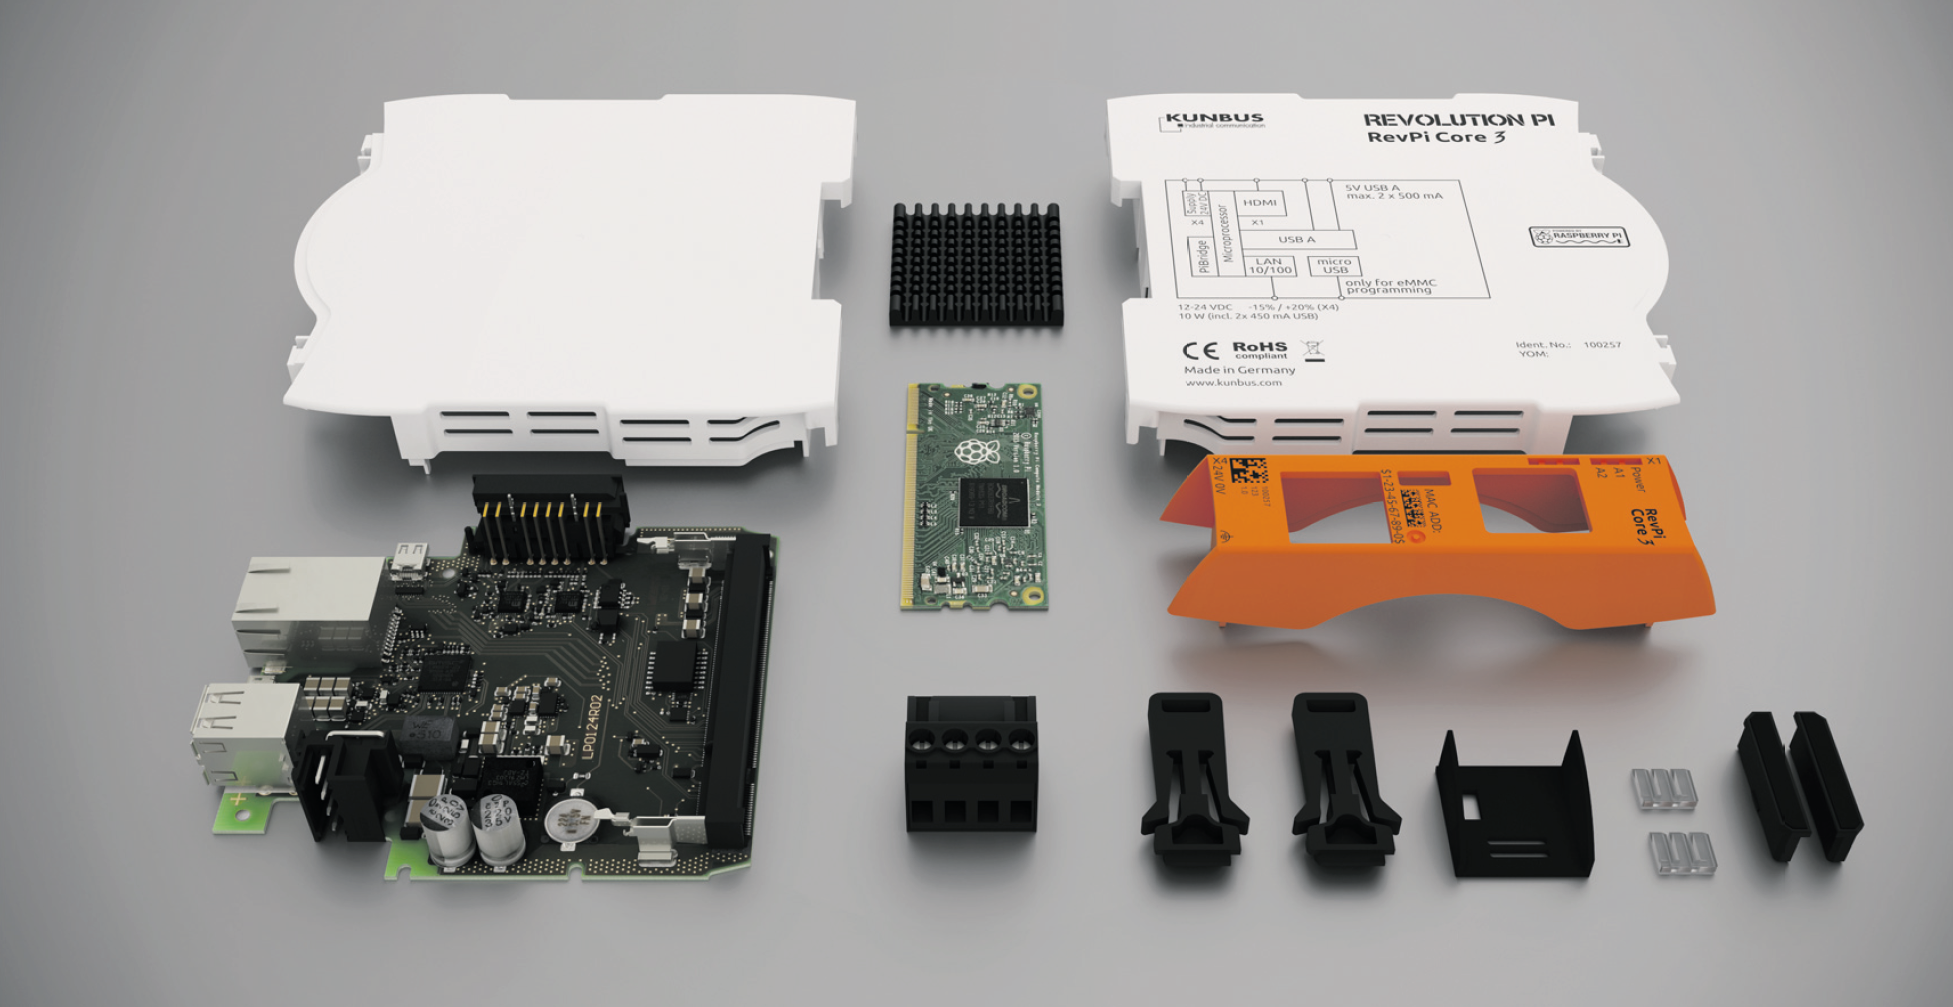
\includegraphics[width=0.85\textwidth]{doc/tex/images/revpi_teardown.png}
    \caption{Der RevPi Core 3 und seine Einzelkomponenten (Quelle: Kunbus)
      \label{fig:revpi-expl}}
\end{figure}

Spezifikationen des RevPi Core 3 \citep[Auswahl, vgl.][S. 1]{datasheet-revpi}:
\begin{itemize}
  \item{Prozessor: BCM2837}
  \item{Taktfrequenz 1,2 GHz}
  \item{Anzahl Prozessorkerne: 4}
  \item{Arbeitsspeicher: 1 GByte}
  \item{eMMC Flash Speicher: 4 GByte}
  \item{Betriebssystem: Angepasstes Raspbian mit RT-Patch}
  \item{RTC mit 24h Pufferung über wartungsfreien Kondensator}
  \item{Treiber / API: Kernel-Treiber schreibt zyklisch Prozessdaten in ein Prozessabbild, Zugriff auf Prozessabbild mittels ioctl-Anfragen oder über Linux-Dateisystem als API zu Fremdsoftware}
  \item{Kommunikationsanschlüsse: 2 x USB 2.0 A, 1 x Micro-USB, HDMI, Ethernet 10/100 Mbit/s}
  \item{Stromversorgung: min. 10,7 V, max. 28,8 V, maximal 10 Watt}
\end{itemize}

Kunbus stellt für den Revolution Pi ein auf Raspbian\footnote{Raspbian ist eine speziell 
für den Raspberry Pi angepasste Variante von Debian.} Stretch basierendes Betriebssystem bereit.
Verwendet wird der Kernel 4.9.76-rt60-v7+ in Verbindung mit dem SMP PREEMPT RT Patch.

\begin{figure}
    \centering
    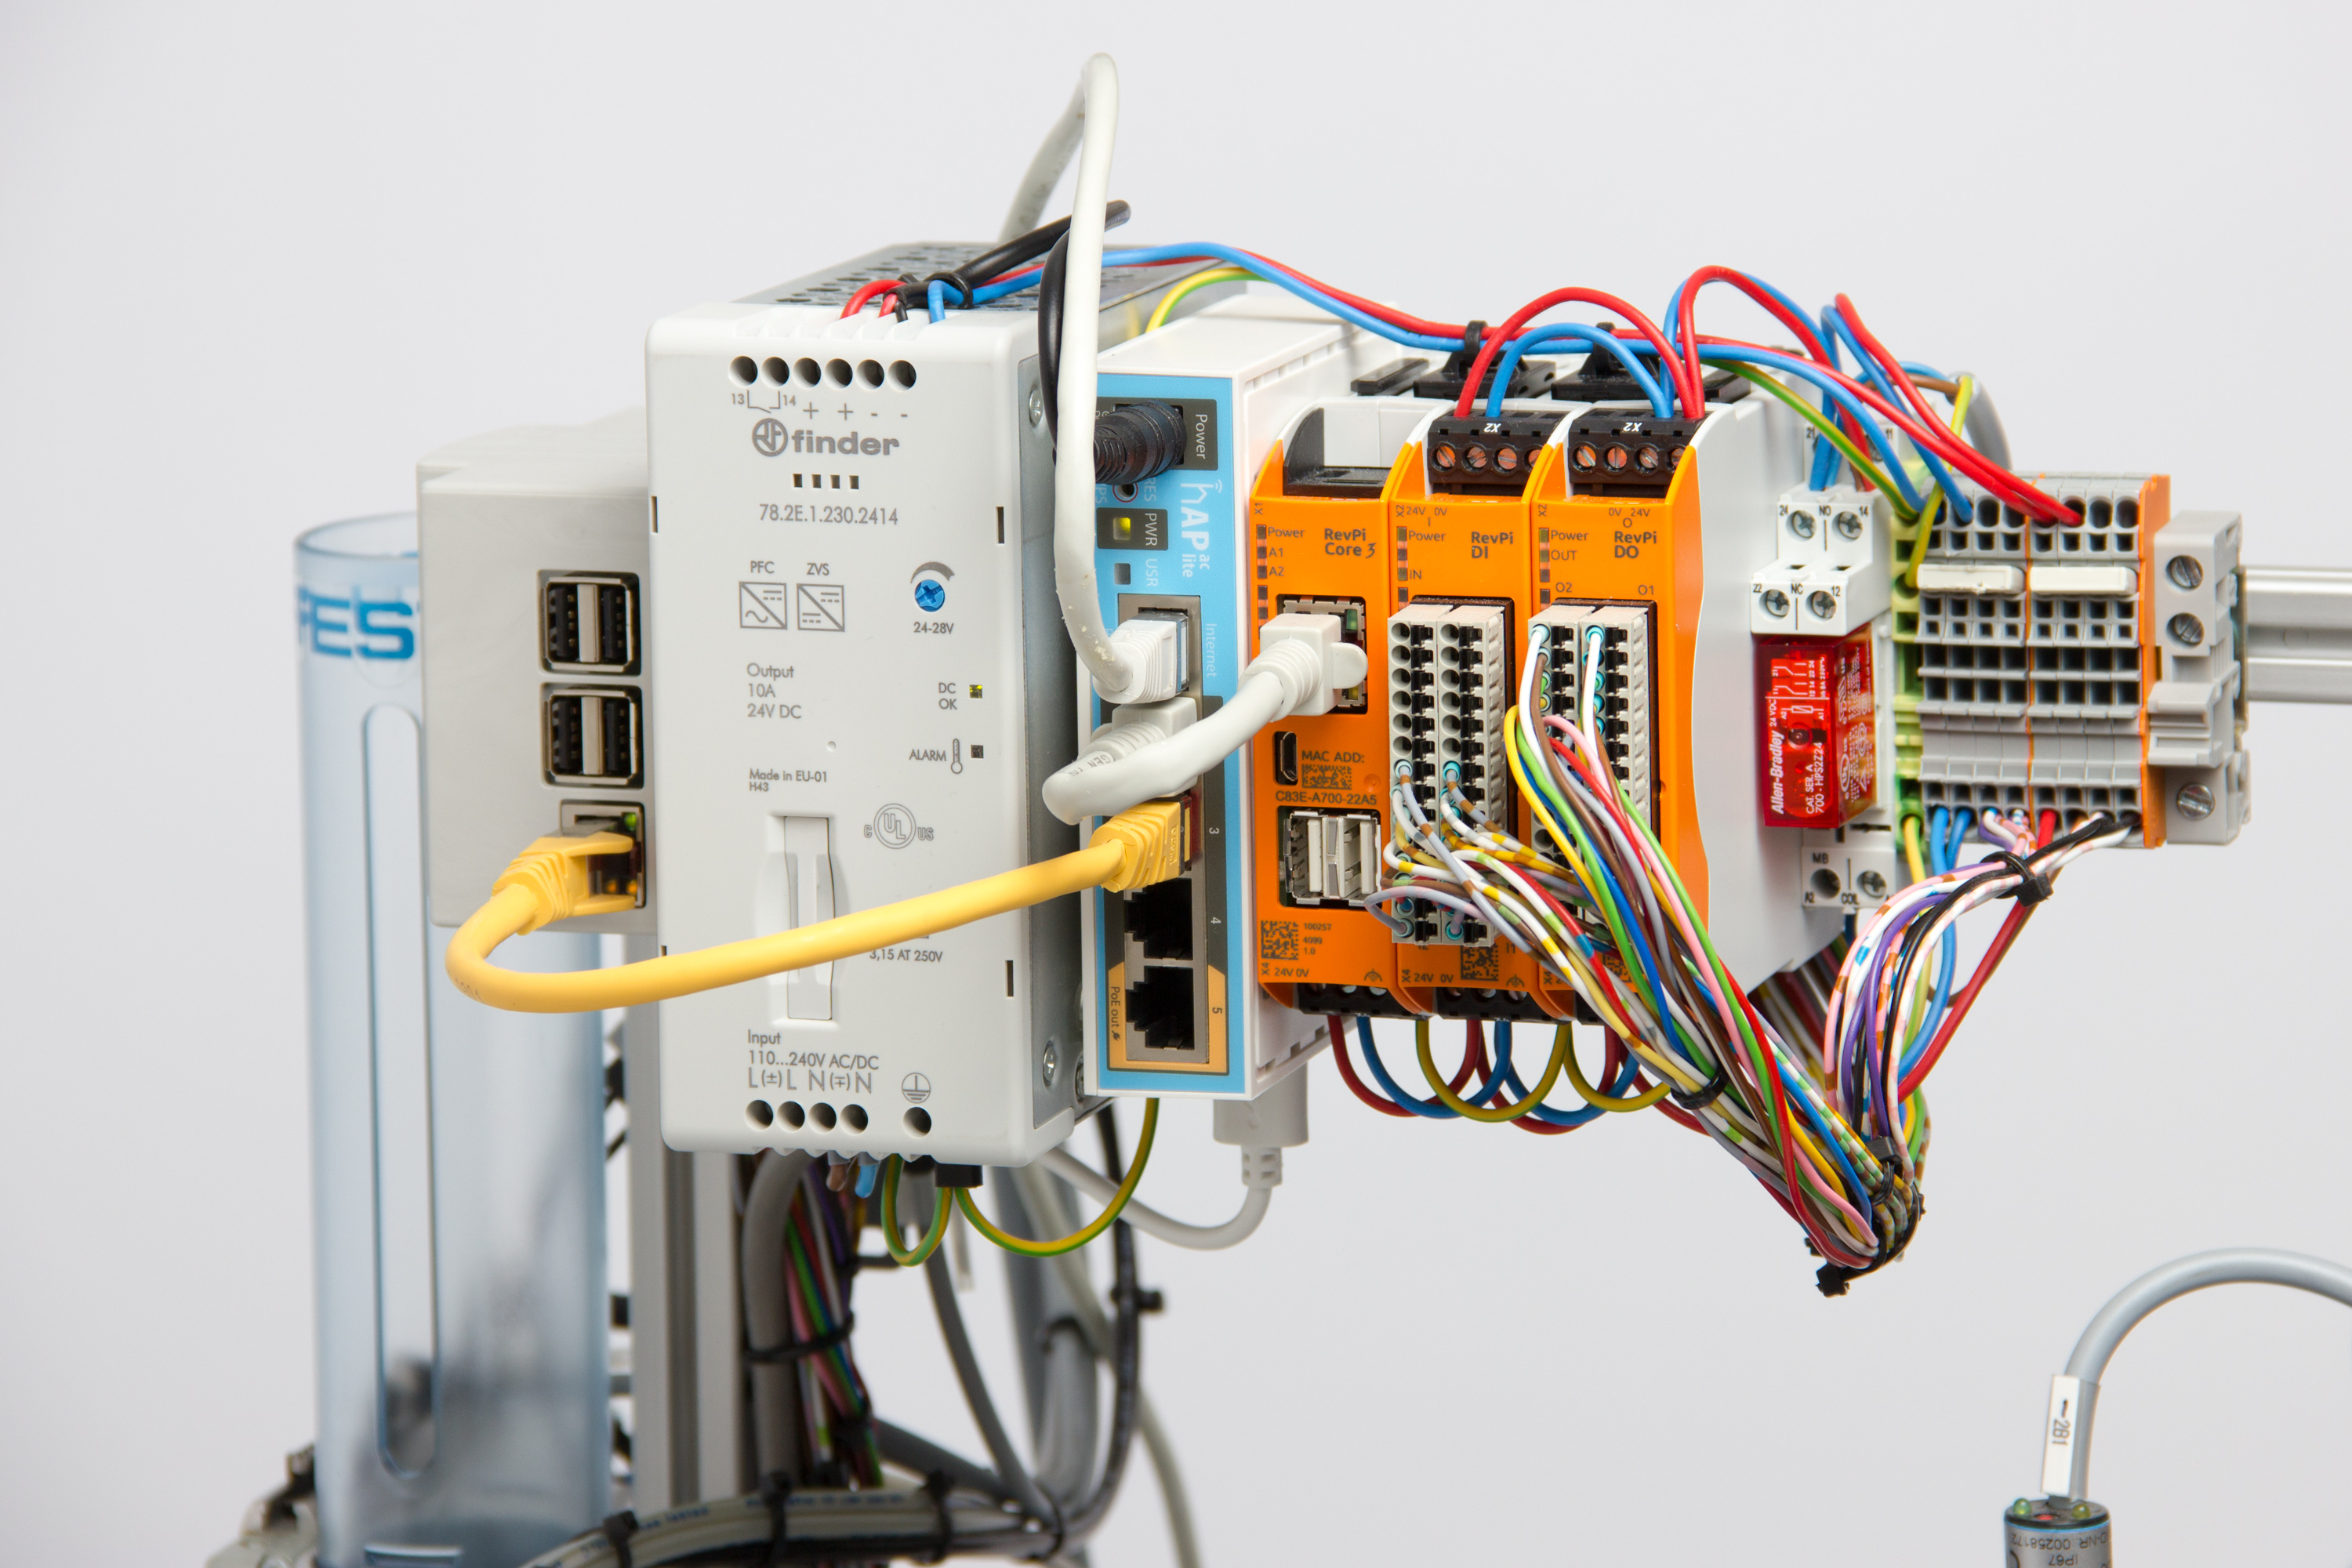
\includegraphics[trim={13cm 5cm 1cm 3cm}, clip, width=0.85\textwidth]{../photos/serverless_plc_img_8}
    \caption{Der Revolution Pi 3 mit digitalen IO-Modulen}
    \label{fig:rev-pi-io}
\end{figure}

Kunbus bietet neben dem sog. Core auch IO- und Gateway-Modulen zur Erweiterung der SPS an, siehe Bild~\ref{fig:rev-pi-io}.
Gateways dienen der Kommunikation mit externen Systemen oder Komponenten
über in der Automatisierungstechnik gängige Protokolle wie PROFIBUS oder EtherCAT. 
IO-Module erlauben die Überwachung und Steuerung von digitalen oder analogen Ein- und Ausgängen (IOs).

Kunbus deklariert die Hardware des Revolution Pi als Open-Source \citep[vgl.][S. 4]{flyer-revpi}. 
Die Schaltpläne des Revolution Pi, genauer die des RevPi Core 3 und der IO-Module, stehen auf der
Website\footnote{\label{downloads}\url{https://revolution.kunbus.com/tutorials/downloads/}} des Herstellers zum 
Download bereit. Eine Lizenz wird nicht angegeben.
Die Raspberry Pi Foundation stellt die Schaltpläne des Compute Modules des weiteren in ihrem Gitub-Repository 
zum Download bereit.

Sowohl die Raspberry Pi Foundation als auch die Kunbus GmbH pflegen aktiv ihre öffentlichen Repositories\footnote{\url{https://github.com/raspberrypi/} resp.~\url{https://github.com/RevolutionPi/}}
auf Github. 

% Kunbus konnte so einige Verbesserungen zum Linux Kernel 4.15 beitragen
% \footnote{siehe \url{https://revolution.kunbus.com/our-contribution-to-linux-4-15/}}.
% \todo{letzten Absatz evtl. weglassen? an sich nicht schlecht, passt aber irgendwie 
% nicht richtig zum Rest und stört den Lesefluss}

\subsubsection{Zugriff auf IO-Module%
        \label{sec:2-io}}
Der Zugriff auf die Ein- und Ausgänge der IO-Module erfolgt über einen RS485-Bus und einen in Form eines Kernel-Moduls bereitgestellten Treiber, genannt piControl. Der RS485-Bus ist über die serielle Schnittstelle des Compute Modules angebunden. 
piControl stellt ein Prozessabbild bereit, welches den physikalischen Zustand der Ein- und Ausgänge der IO-Module repräsentiert.
Das Prozessabbild wird, wie in der Automatisierungstechnik üblich, zyklisch aktualisiert. 
Die angestrebte Zykluszeit beträgt 5ms, kann jedoch je nach Anzahl der angeschlossenen Module auch größer sein. 
Kunbus garantiert bei drei IO-Modulen und zwei Gateway-Modulen eine Zykluszeit von 10 ms \citep[vgl.][]{web-revpi-dio}.
Die garantierte Zykluszeit ermöglicht die Umsetzung von Anwendungen mit harten Echtzeit-Anforderungen.

Fremdanwendungen können über eine Applikationsschnittstelle (API) auf das Prozessabbild zugreifen. 
Hierzu stellt das Kernel-Modul piControl sowohl \lstinline{seek}, \lstinline{read} und \lstinline{write} Methoden zur verfügung, wie auch die Möglichkeit mittels \lstinline{ioctl}-Anfragen gezielt auf einzelne Variablen des Prozessabbildes zuzugreifen.
In der englischsprachigen Wikipedia werden ioctl-Aufrufe wie folgt beschrieben:

\glqq{}The kernel is designed to be extensible, and may accept an extra module called a device driver which runs in kernel space and can directly address the device. An ioctl interface is a single system call by which userspace may communicate with device drivers. [...] The basic kernel can thus allow the userspace to access a device driver without knowing anything about the facilities supported by the device, and without needing an unmanageably large collection of system calls.

[...] ioctl calls provide a convenient way to bridge userspace code to kernel extensions. Kernel extensions can provide a location in the filesystem that can be opened by name, through which an arbitrary number of ioctl calls can be dispatched, allowing the extension to be programmed without adding system calls to the operating system.\grqq{}\citep[vgl.][]{web-wiki-ioctl}

Der Quellcode von piControl steht unter der GNU General Public License Version 2 (GNU GPLv2) und ist 
auf Github verfügbar\footnote{\url{https://github.com/RevolutionPi/piControl}}. Als Einstieg in die 
Entwicklung eigener Steuerungsprogramme liefert Kunbus das C-Programm piTest mit. Dieses verwendet 
piControl und erlaubt dem Nutzer über Kommandozeilen-Parameter die angeschlossenen IO-Module zu steuern.

\begin{figure}[h]
    \centering
    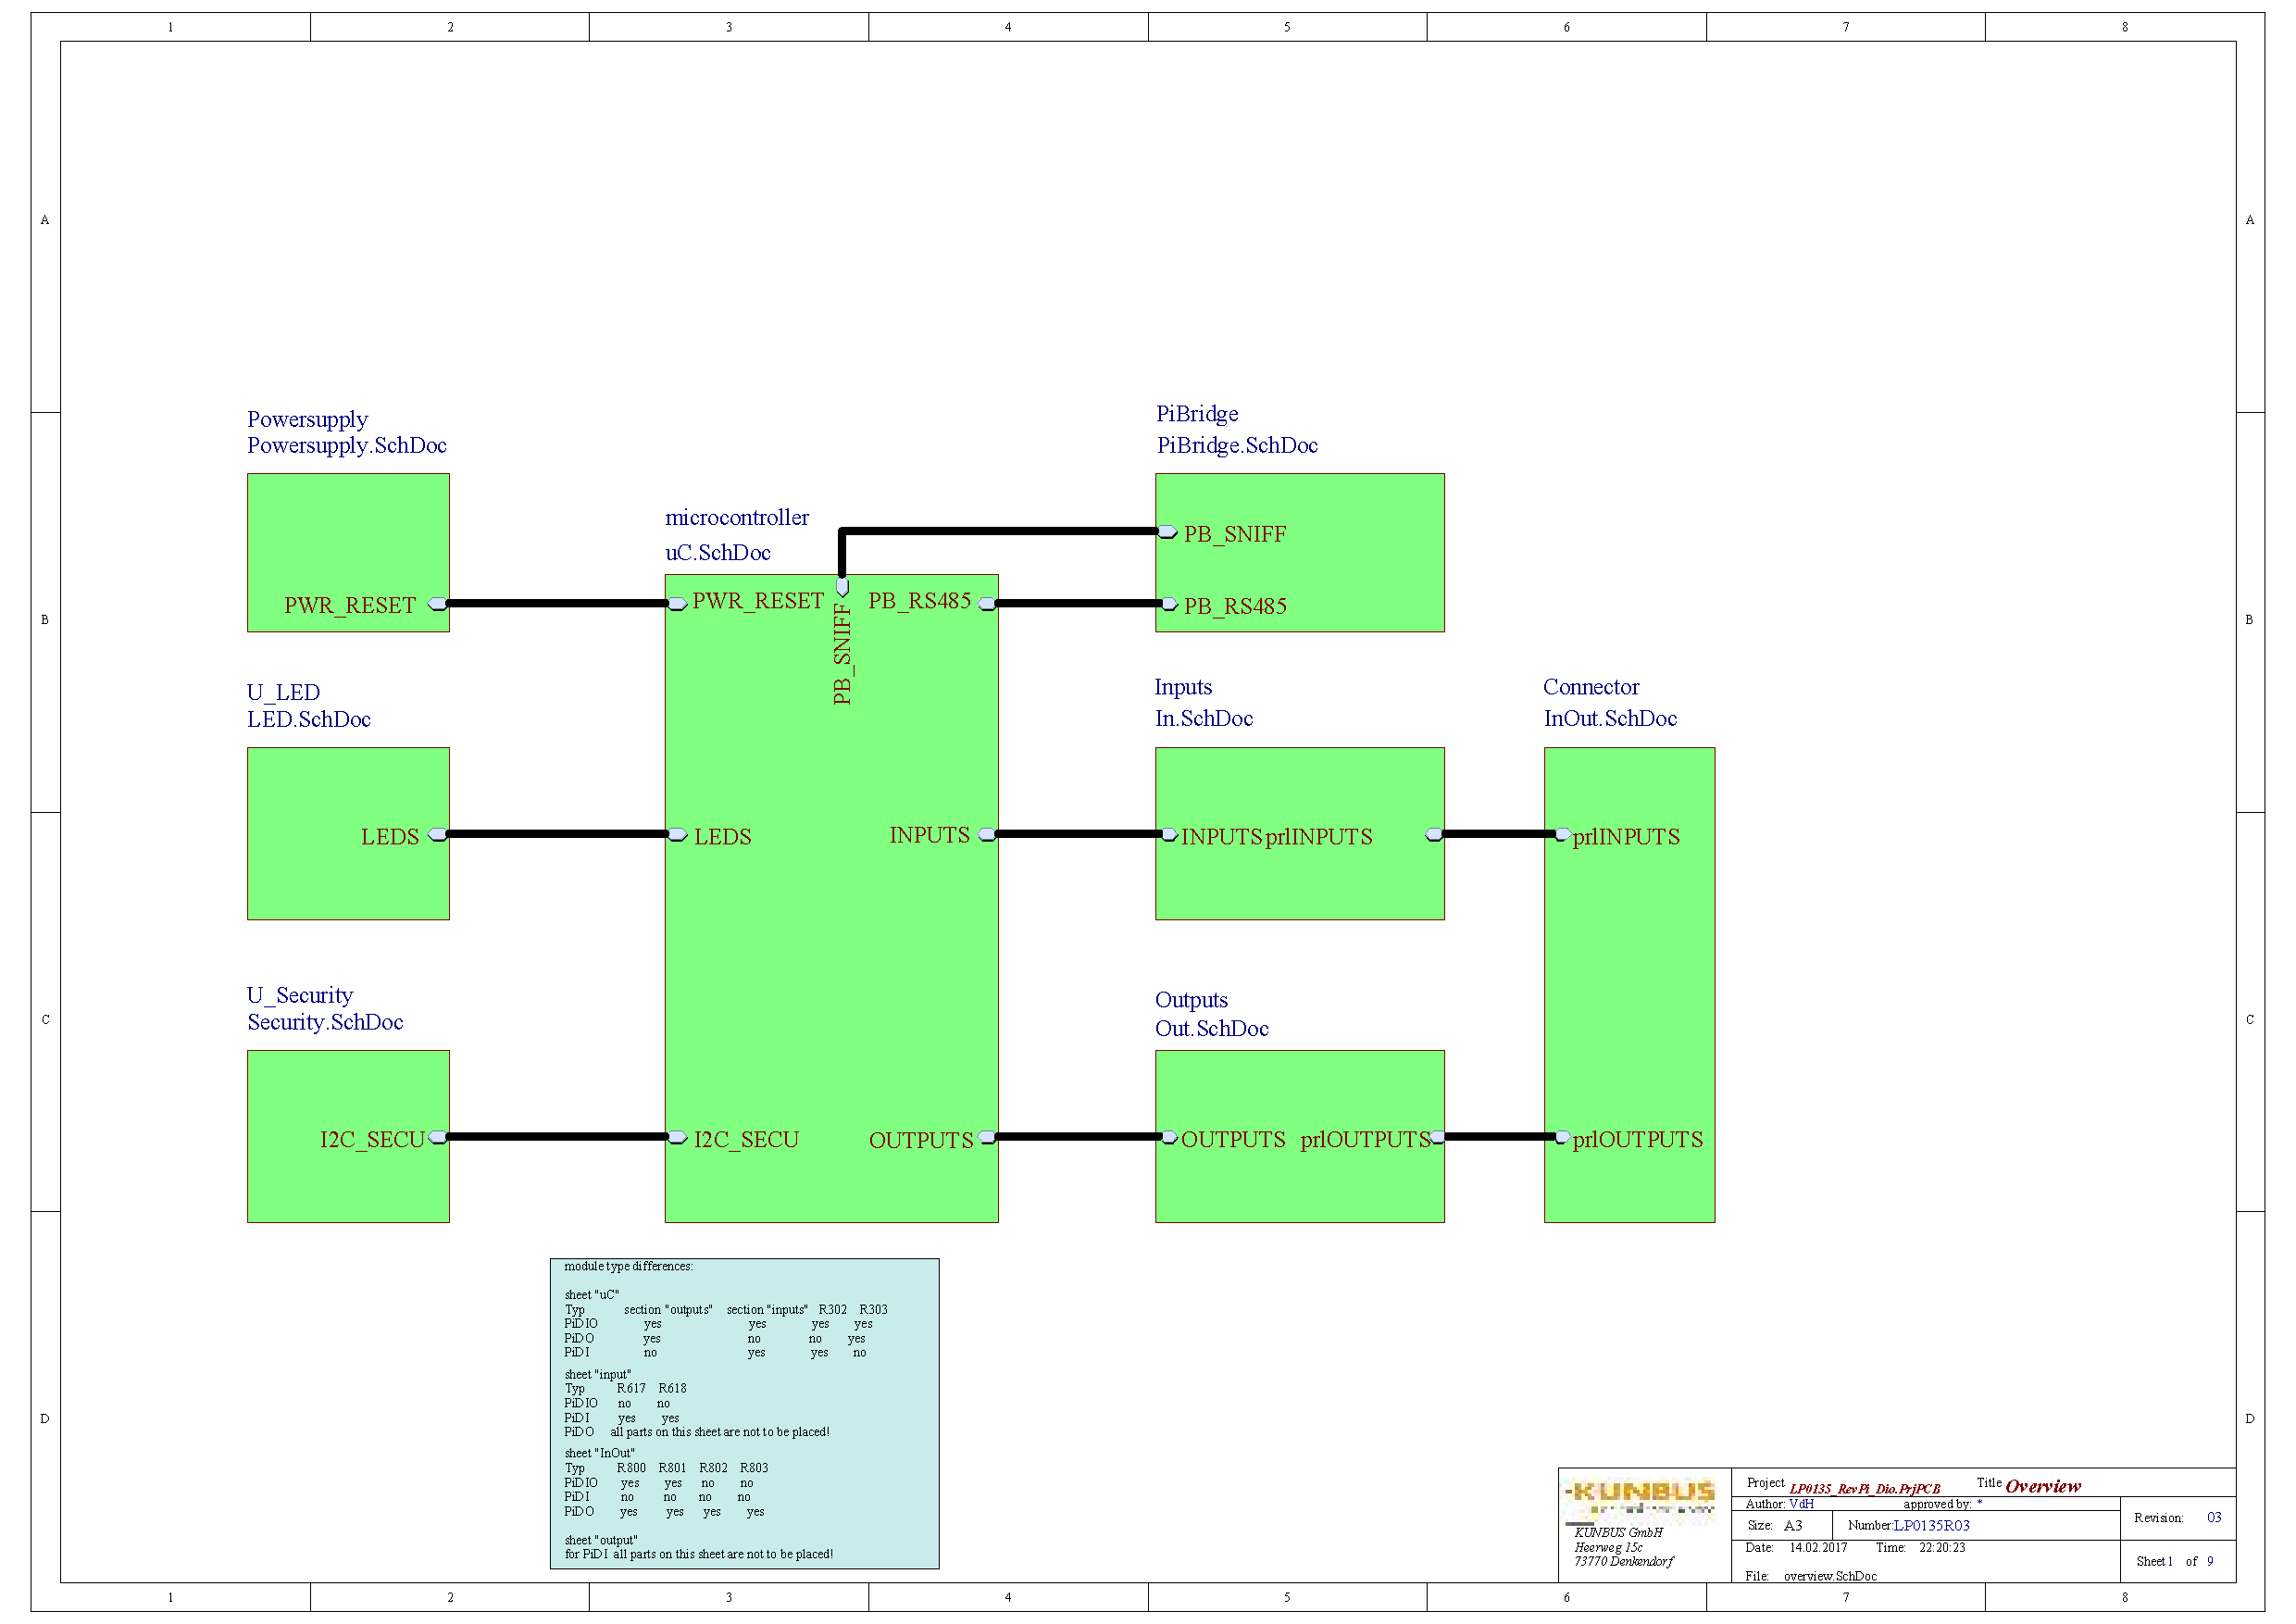
\includegraphics[trim={4cm 7cm 10.5cm 7.3cm}, clip, width=\textwidth]{literature/SchematicPrintsRevPi-DIO}
    \caption{Schematische Darstellung eines DIO-Moduls (Quelle: Kunbus\textsuperscript{\ref{downloads}})
      \label{fig:dio}}
\end{figure}

Jedes der IO-Module stellt ein eigenständiges eingebettetes System dar. Es verfügt
über einen Microcontroller, welcher die IOs bereitstellt und über einen RS485-Bus
mit dem Revolution Pi kommuniziert (siehe Bild~\ref{fig:dio}). 
Kunbus stellt exemplarisch den Quellcode eines DIO-Moduls unter der MIT Lizenz zur
Verfügung\footnote{\url{https://github.com/RevolutionPi/IODeviceExample}}. 


\subsection{Echtzeit und Multitasking unter Linux -- preemptRT und posix%
     \label{sec:2-echtzeit}}
     
Moderne Betriebssysteme realisieren Multitasking i.d.R.\,in Form des präemptiven Multitasking. 
Der Kernel verfügt über einen sog. Scheduler. Dieser priorisiert alle Prozesse und weist ihnen 
Rechenzeit in sog. Time Slots zu. Die Größe der Zeitfenster sowie die Ausführungsreihenfolge 
ist von der Priorität eines Prozesses abhängig. Besonders an einem präemptiven im Gegensatz zu einem kooperativen Scheduler ist dessen Fähigkeit, Tasks während ihrer Ausführung zu unterbrechen bzw. zu pausieren, wenn diese eine bestimmte Dauer überschreiten oder ein höher priorisierter Prozess (bspw. ausgelöst durch einen Interrupt oder durch eine inhärente Periodizität) Rechenleistung benötigt.

Eine Sonderform des präemptiven Multitasking ist das präemptible Multitasking. Hierbei werden auch Teile 
des Kernels als Threads durch den Scheduler ausgeführt. Dieser ist somit in der Lage, auch Prozesse des Kernels
zu unterbrechen, wenn andere Anwendungen Prozessorzeit oder Zugriff auf andere Systemressourcen benötigen
\citep[vgl.][]{web-wiki-praempt}.
     
Der Linux-Kernel implementiert unterschiedliche Präemptions-Modelle \citep[vgl.][/preemption\_models]{web-linuxwiki-basics}:

\begin{itemize}
  \item No Forced Preemption (server):
  Ausgelegt auf maximal möglichen Durchsatz, lediglich Interrupts und
  System-Call-Returns bewirken Präemption.

  \item Voluntary Kernel Preemption (Desktop):
  Neben den implizit bevorrechtigten Interrupts und System-Call-Returns gibt es
  in diesem Modell weitere Abschnitte des Kernels in welchen Preämption explizit
  gestattet ist.

  \item Preemptible Kernel (Low-Latency Desktop):
  In diesem Modell ist der gesamte Kernel, mit Ausnahme sog.~kritischer Abschnitte
  präemptible. Nach jedem kritischen Abschnitt gibt es einen impliziten Präemptions-Punkt.

  \item Preemptible Kernel (Basic RT):
  Dieses Modell ist dem zuvor genannten sehr ähnlich, hier sind jedoch alle Interrupt-Handler
  als eigenständige Threads ausgeführt.

  \item Fully Preemptible Kernel (RT):
  Wie auch bei den beiden zuvor genannten Modellen ist hier der gesamte Kernel
  präemtible. Die Anzahl und Dauer der nicht-präemtiblen kritischen Abschnitte
  ist auf ein notwendiges Minimum beschränkt. Alle Interrupt-Handler sind als
  eigenständige Threads ausgeführt, Spinlocks durch Sleeping-Spinlocks und Mutexe
  durch sog.~RT-Mutexe ersetzt.

\end{itemize}

Lediglich ein präemtibler Kernel kann hartes Echtzeit-Verhalten realisieren, 
da nur hier eine maximale Antwortzeit garantiert werden kann.
Viele Prozesse in der Automatisierungstechnik erfordern harte Echtzeit. 
Eine verspätete Antwort auf eine Anfrage, 
wie etwa das Signal eines Lagenendschalters oder eines Notausschalters kann hier nicht nur über
den Erfolg eines Prozesses, sondern auch über das Leben der daran beteiligten Mitarbeiter entscheiden.
Für weiterführende Erklärungen bzgl.\,Echtzeit, Mutexen und 
Spinlocks sei an dieser Stelle auf die Vorlesung verwiesen~\citep{script-peter}.


\subsubsection{preemptRT%
        \label{sec:2-preemptRT}}

Der Kernel des auf dem Revolution Pi installierten Raspbian mit PREEMP\_RT Patch fällt 
in die Kategorie des \glqq{}Fully Preemptible Kernels\grqq{} (siehe Abschnitt \ref{sec:2-echtzeit}).
Das zugrunde liegende Prinzip lässt sich wie folgt formulieren: Nur Code, welcher absolut nicht-präemtible sein darf, ist es
gestattet nicht-präemtible zu sein. Ziel ist folglich, die Menge des nicht-präemtiblen 
Codes im Linux-Kernel auf das absolut notwendige Minimum zu reduzieren.

Dies wird durch Verwendung folgender Mechanismen erreicht~\citep[vgl.][]{web-linuxwiki-details}:

\begin{itemize}
  \item Hochauflösende Timer
  \item Sleeping Spinlocks
  \item Threaded Interrupt Handlers
  \item rt\_mutex
  \item RCU
\end{itemize}

Diese Mechanismen sind bspw. im Linux-Wiki\footnote{siehe \url{https://wiki.linuxfoundation.org/realtime/documentation/technical_details}} ausführlich beschrieben.

\subsubsection{POSIX%
        \label{sec:2-posix}}
Das Portable Operating System Interface (POSIX) bezeichnet eine Sammlung von Standards, 
welche auf dem Unix-System basieren, jedoch nicht auf dieses beschränkt sind.

Der Wechsel zwischen verschiedenen Unix-Distributionen brachte oft Kompatibilitätsprobleme mit sich. 
Dieser Mangel an Portabilität erschwerte Benutzern und Entwicklern die Verwendung bzw. Bereitstellung 
von Software auf unterschiedlichen Systemen. 
Das Institut für Elektrotechnik und Elektronik (IEEE) begann 1984 mit der Entwicklung des Unix-Standards.
Sie entwickelten das, was heute als Single UNIX Specification bekannt ist und allgemein als POSIX bezeichnet wird~\citep[vgl.][]{web-debianwiki-posix}.
Das Konsortium \glqq{}The Open Group\grqq{} überwacht die weitere Entwicklung dieses Standards.
Ferner stellt es einen Teil der POSIX-Spezifikation frei zur Verfügung~\citep[vgl.][]{web-opengroup-posix}.

Die aktuelle Version POSIX.1-2017 ist verfügbar als IEEE Standard 1003.1-2017 sowie in Form der \glqq{}The Open Group Technical Standard Base Specifications\grqq{}, Ausgabe 7. POSIX.1-2017 definiert eine Standard-Betriebssystemschnittstelle und -umgebung, einschließlich eines Befehlsinterpreters (auch Shell genannt) und gängiger Dienstprogramme zur Unterstützung der Portabilität von Anwendungen auf Quellcode-Ebene. POSIX.1-2017 ist sowohl für Anwendungsentwickler als auch für Systemimplementierer gedacht und umfasst vier Hauptkomponenten \citep[vgl.][]{web-opengroup-overview}:
\begin{itemize}
    \item Basisdefinitionen:\\
          Allgemeine Begriffe, Konzepte und Schnittstellen einschließlich Hilfskonventionen und C-Headern
          
    \item Systemschnittstellen:\\
          Definitionen für Systemdienstfunktionen und Unterprogramme, C-spezifische Systemdienste, Portabilität
        
    \item Shell und Dienstprogramme:\\
          Definitionen für eine Schnittstelle zur Befehlsinterpretation von Diensten und gängige Hilfsprogramme
    
    \item Begründungen und Historie
\end{itemize}

Debian basiert auf Linux und verwendet den Linux-Kernel. Linux ist zu großen Teilen POSIX-kompatibel. Debian ist jedoch nicht POSIX-zertifiziert, da diese Zertifizierung mit hohen Kosten verbunden ist\citep[vgl.][Kapitel 4.4.]{web-debian-faq}.

Beide Kernkomponenten des in dieser Arbeit vorgestellten Projektes nutzen Komponenten von Linux, 
welche an den POSIX-Standard angelehnt sind: open62541 verwendet u.a.\,POSIX-Threads und
Mutexe~\citep[vgl.][pthread.h]{web-opengroup-pthread}, piControl nutzt POSIX-Semaphoren
\citep[vgl.][semaphore.h]{web-opengroup-semaphore}. 


\subsection{OPC-UA und open62541%
     \label{sec:2-opc}}
In diesem Abschnitt sollen Möglichkeiten des Datenaustausch zwischen Komponenten der
Automatisierungstechnik vorgestellt werden. OPC-UA stellt einen offenen, IP-basierten Kommunikationsstandard
für Sensoren und Steuerungen dar. open62541 ist eine freie Client- sowie Server-Implementierung dieses
Standards, geschrieben in C.


\subsubsection{OPC UA%
        \label{sec:2-opcua}}

Open Platform Communications (OPC) ist eine Familie von Standards zur herstellerunabhängigen
Kommunikation von Maschinen (M2M) in der Automatisierungstechnik. Die sog. OPC Task Force, zu deren
Mitgliedern verschiedene etablierte Firmen der Automatisierungsindustrie gehören, veröffentlichte
die OPC Specification Version 1.0 im August 1996.
Motiviert ist dieser offene Standard durch die Erkenntniss, dass die Anpassung der
zahlreichen Herstellerstandards an individuelle Infrastrukturen und Anlagen einen
großen Mehraufwand verursachen.
Die Wikipedia beschreibt das Anwendungsgebiet für OPC wie folgt \citep[vgl.][]{web-wiki-opc}:

\glqq{}OPC wird dort eingesetzt, wo Sensoren, Regler und Steuerungen verschiedener Hersteller
ein gemeinsames Netzwerk bilden. Ohne OPC benötigten zwei Geräte zum Datenaustausch
genaue Kenntnis über die Kommunikationsmöglichkeiten des Gegenübers. Erweiterungen
und Austausch gestalten sich entsprechend schwierig. Mit OPC genügt es, für jedes
Gerät genau einmal einen OPC-konformen Treiber zu schreiben. Idealerweise wird
dieser bereits vom Hersteller zur Verfügung gestellt. Ein OPC-Treiber lässt sich
ohne großen Anpassungsaufwand in beliebig große Steuer- und Überwachungssysteme
integrieren.

OPC unterteilt sich in verschiedene Unterstandards, die für den jeweiligen Anwendungsfall
unabhängig voneinander implementiert werden können. OPC lässt sich damit verwenden
für Echtzeitdaten (Überwachung), Datenarchivierung, Alarm-Meldungen und neuerdings
auch direkt zur Steuerung (Befehlsübermittlung).\grqq{}

OPC basiert in der ursprünglichen Spezifikation (auch als OPC DA bezeichnet) auf Microsofts DCOM-Spezifikation.
DCOM macht Funktionen und Objekte einer Anwendung anderen Anwendungen im Netzwerk
zugänglich. Der OPC-Standard definiert entsprechende DCOM-Objekte um mit anderen
OPC-Anwendungen Daten austauschen zu können. Die Verwendung von DCOM bindet Anwender
jedoch an Betriebssysteme von Microsoft. 

\begin{figure}
    \centering
    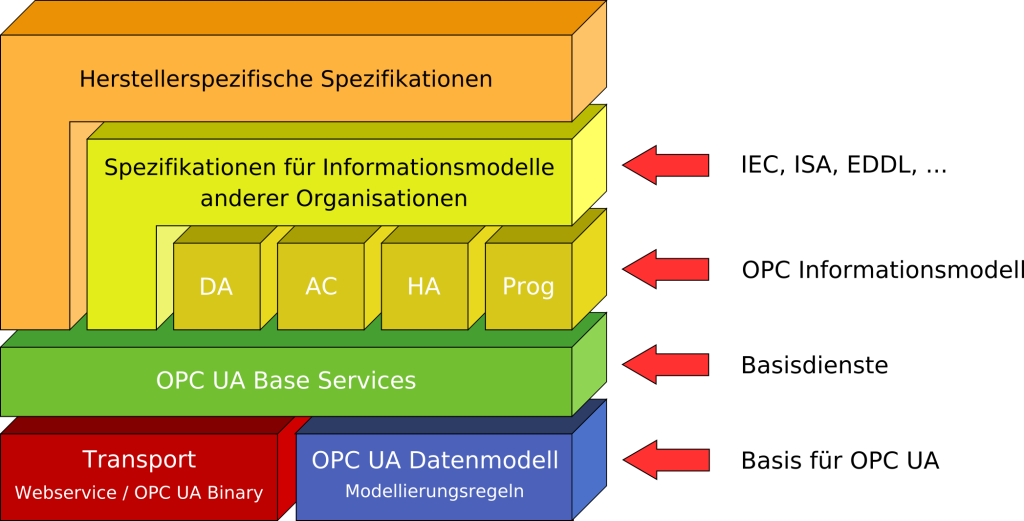
\includegraphics[width=0.85\textwidth]{images/UA_Architecture_1024.png}
    \caption{Die OPC Unified Architecture. Grafik von Gerhard Gappmeier - ascolab GmbH, CC BY-SA 3.0}
    \label{fig:opc-unified-architecture}
\end{figure}
% Evtl Grafik: Von Gerhard Gappmeier - ascolab GmbH, CC BY-SA 3.0, https://de.wikipedia.org/w/index.php?curid=1892069

Die ursprüngliche OPC Spezifikation wurde 2006 durch die Entwicklung der 
OPC Unified Architecture (OPC UA) überholt. 
Diese zeichnet sich durch eine Service-orientierte Architektur (SOA) aus, deren Struktur
aus mehreren Schichten besteht, siehe Abbilung~\ref{fig:opc-unified-architecture}. 
Über der untersten Schicht, dem Betriebssystem des Servers, verbindet eine Portabilitäts-Schicht 
den sog.\, UA ANSI C Stack mit einer API. Diese API kann bspw.\,in C++ geschrieben sein, 
und erlaubt die Anbindung der obersten Schicht, der Anwendungsschicht~\citep[vgl.][]{web-spec-opc}.
OPC UA setzt auf einem eigenen Kommunikationsstack auf; die Verwendung von DCOM
und damit die Bindung an Microsoft wurden aufgelöst.

Neben Architektur und Kommunikationsschnittstellen wird in der OPC Spezifikation auch ein 
Informationsmodell definiert. Die deutschsprachige Wikipedia beschreibt dieses wie folgt: 

\glqq{}Das OPC[-UA]-Informationsmodell ist nicht mehr nur eine Hierarchie aus Ordnern, Items
und Properties. Es ist ein sogenanntes Full-Mesh-Network aus Nodes, mit dem neben
den Nutzdaten eines Nodes auch Meta- und Diagnoseinformationen repräsentiert werden. [...]
Ein Node ähnelt einem Objekt aus der objektorientierten Programmierung. Ein Node
kann Attribute besitzen, die gelesen werden können. Es ist möglich Methoden zu definieren und aufzurufen. [...]
Weiterhin werden Events unterstützt, die versendet werden können
(AE (Alarms \& Events), DA DataChange), um bestimmte Informationen zwischen Geräten
auszutauschen. Ein Event besitzt unter anderem einen Empfangszeitpunkt, eine Nachricht
und einen Schweregrad. Die o.\,g. Nodes werden sowohl für die Nutzdaten als auch
alle anderen Arten von Metadaten verwendet. Der damit modellierte OPC-Adressraum
beinhaltet nun auch ein Typmodell, mit dem sämtliche Datentypen spezifiziert werden.\grqq{}


\subsubsection{open62541%
        \label{sec:2-open62541}}
open62541 ist eine offene und freie Implementierung von OPC UA. 
Die in C geschriebene Bibliothek stellt eine beständig zunehmende Anzahl der im OPC UA Standard definierten
Funktionen bereit. Sie kann sowohl zur Erstellung von OPC-Servern als auch von -Clients
genutzt werden. Ergänzend zu der unter der Mozilla Public License v2.0 lizensierten
Bibliothek stellt das open62541 Projekt auch Beispielprogramme unter einer CC0 Lizenz
zur Verfügung.
Zu den Unterstützern des Projektes zählen u.a.\, die RWTH Aachen, das Frauenhofer IOSB sowie die TU Dresden.

Die Bibliothek eignet sich auch für die Entwicklung auf eingebetteten Systemen und
Microcontrollern. Die Größe einer Server-Binary kann weniger als 100kB betragen.

Folgende Auswahl an Eigenschaften und Funktionen zeichnet die in dieser Arbeit verwendete
Version 0.3 von open62541 aus:
\begin{itemize}
  \item Kommunikationionsstack
  \begin{itemize}
      \item OPC UA Binär-Protokoll (HTTP oder SOAP werden gegenwärtig nicht unterstützt)
      \item Austauschbare Netzwerk-Schicht, welche die Verwendung eigener Netzwerk-APIs
      erlaubt.
      \item Verschlüsselte Kommunikationion
      \item Asynchrone Dienst-Anfragen im Client
  \end{itemize}
  \item Informationsmodell
  \begin{itemize}
    \item Unterstützung aller OPC UA Node-Typen, inkl.~Methoden
    \item Hinzufügen und Entfernen von Nodes und Referenzen zur Laufzeit.
    \item Vererbung und Instanziierung von Objekt- und Variablentypen
    \item Zugriffskontrolle auch für einzelne Nodes
  \end{itemize}
  \item Subscriptions
  \begin{itemize}
    \item Erlaubt die Überwachung (subscriptions / monitoreditems)
    \item Sehr geringer Ressourcenbedarf pro überwachtem Wert
  \end{itemize}
  \item Code-Generierung auf XML-Basis
  \begin{itemize}
    \item Erlaubt die Erstellung von Datentypen
    \item Erlaubt die Generierung des serverseitigen Informationsmodells
  \end{itemize}
\end{itemize}

Weiterführende Informationen und Code-Beispiele bietet die ausführliche Dokumentation des Projektes~\citep[siehe]{web-open62541} sowie der kommentierte Quelltext.

%% % Imports nur für Referenzenauflösung während des Schreibens! Vorm Kompilieren auskommentieren!
% \bibliography{0_hauptdatei}
% \input{1_einleitung}
% \input{2_grundlagen}
% \input{3_konzeption}
% \input{4_implementierung}
% \input{5_tests}
% \input{6_zusammenfassung}
% \input{anhang}
% % Ende Imports

\section{Systemkonzept%
  \label{sec:3-konzeption}}
Auf Basis der in Abschnitt [...] vorgestellten Möglichkeiten folgt nun die Ausarbeitung eines Konzepts.

\subsection{Anbindung der IO an den OPC-Server%
     \label{sec:3-anbindung}}

\subsection{Integration des OPC-Servers in das System%
     \label{sec:3-integration}}

%% % Imports nur für Referenzenauflösung während des Schreibens! Vorm Kompilieren auskommentieren!
% \bibliography{0_hauptdatei}
% \input{1_einleitung}
% \input{2_grundlagen}
% \input{3_konzeption}
% \input{4_implementierung}
% \input{5_tests}
% \input{6_zusammenfassung}
% \input{anhang}
% % Ende Imports

\section{Implementierung%
  \label{sec:4-implementierung}}
Das folgende Kapitel stellt in Auszügen die Implementierung des OPC-Servers sowie die Anbindung an die IO-Module
der SPS dar. Der Schwerpunkt liegt hierbei auf der Funktionsweise des piControl-Treibers und dessen Integration in das Projekt. Abschnitt~\ref{sec:4-picontrol} erklärt die zum Schreibens eines Bits verwendeten Funktionsaufrufe.
Zuvor soll jedoch in Abschnitt~\ref{sec:4-open62541} der Teil des OPC-Servers vorgestellt werden, welcher auf besagten Treiber zugreift. 

\subsection{Implementierung des OPC-Servers%
     \label{sec:4-open62541}}
Wie im vorangegangenen Abschnitt~\ref{sec:3-integration} begründet, soll die Verknüpfung zwischen dem Prozessabbild der SPS und den auf dem OPC-Server bereitgestellten Werten über sog.\,Datenquellen erfolgen. Hierzu ist zunächst eine Callback-Methode zu implementieren, welche bei einem Lese- oder Schreibzugriff auf eine Variable aufgerufen wird. Die Verknüpfung zwischen Callback-Methode und Variable muss manuell erfolgen.

\begin{lstlisting}[language={c},firstnumber=237,caption={Auszug der Methode \lstinline{linkDataSourceVariable} in \lstinline{variables.c}\label{lst:4-linkDataSourceVariable}}]
extern UA_StatusCode
 linkDataSourceVariable(UA_Server *server, UA_NodeId nodeId) {
     bool readonly = false;
     UA_DataSource dataSourceVariable;
     UA_StatusCode rc; |>\setcounter{lstnumber}{254}<|

     dataSourceVariable.read = readDataSourceVariable;
     if (!readonly)
        dataSourceVariable.write = writeDataSourceVariable;
     else
        dataSourceVariable.write = writeReadonlyDataSourceVariable;

     return UA_Server_setVariableNode_dataSource(server, nodeId, dataSourceVariable);
 }
\end{lstlisting}

\begin{figure}[h]
    \centering
    \includegraphics[width=0.42\textwidth]{doc/img/OPC_RevPiDO.pdf}
    \caption{Auszug des verwendeten Nodesets, hier Digitalausgang 1 des Versuchsaufbaus
      \label{fig:opc-do}}
\end{figure}

Die in Listing~\ref{lst:4-linkDataSourceVariable} abgebildete Methode \lstinline{linkDataSourceVariable()} erzeugt ein Struct vom Typ \lstinline{UA_DataSource}. In diesem werden dem Lesen und Schreiben einer OPC-Variablen entsprechende Callback-Methoden zugewiesen. Die Verknüpfung einer OPC-Variable, genauer ihrer NodeId, mit der zuvor definierten Datenquelle erfolgt über die von open62541 bereitgestellte Methode \lstinline{UA_Server_setVariableNode_dataSource()}. Vor dem Lesen und nach dem Schreiben dieser Variable werden von nun an die entsprechenden Callbacks aufgerufen.
     
\begin{lstlisting}[language={c},firstnumber=168,caption={Auszug des Callbacks \lstinline{writeDataSourceVariable} in \lstinline{variables.c}\label{lst:4-writeDataSourceVariable}}]  
extern UA_StatusCode
 writeDataSourceVariable(UA_Server *server,
            const UA_NodeId *sessionId, void *sessionContext,
            const UA_NodeId *nodeId, void *nodeContext,
            const UA_NumericRange *range, const UA_DataValue *dataValue) {

    UA_StatusCode retval  = UA_STATUSCODE_GOOD;
    UA_NodeId *nameNodeId = UA_malloc(sizeof(UA_NodeId));
    UA_QualifiedName nameQN = UA_QUALIFIEDNAME(1, "Name");
    UA_Variant nameVar;
    UA_Boolean bit;

    retval |= findSiblingByBrowsename(server, nodeId, &nameQN, nameNodeId);
    retval |= UA_Server_readValue(server, *nameNodeId, &nameVar);
    retval |= UA_Boolean_copy(dataValue->value.data, &bit);

    |>\tikzmarkin[set border color=martinired]{writeIO}<|PI_writeSingleIO(String_fromUA_String(nameVar.data), &bit, false);                                                 |>\tikzmarkend{writeIO}<|

    free(nameNodeId);
    return retval;
 }
\end{lstlisting}

Listing~\ref{lst:4-writeDataSourceVariable} zeigt die Callback-Methode, welche nach dem Schreiben einer Variablen auf dem OPC-Server aufgerufen wird.
Dieser Methode wird neben der NodeId der mit ihr verknüpften Variablen auch der Wert dieser in Form eines Zeigers auf ein Struct vom Typ \lstinline{UA_DataValue} übergeben.

Die Gestaltung des hier verwendeten Nodesets sieht vor, dass in einer OPC-Variablen \lstinline{"Name"} der Bezeichner des zu schreibenden Digitalausgangs hinterlegt ist, siehe Abbildung~\ref{fig:opc-do}. Dies erlaubt eine Rekonfiguration der Ein- und Ausgänge der SPS ohne Änderungen im Programmcode des OPC-Servers vornehmen zu müssen.
Es ist daher erforderlich, nach jedem Schreiben einer mit einem Digitalausgang verknüpften Variablen, hier \lstinline{"Value"}, dessen Bezeichner \lstinline{"Name"} abzufragen. 
Dies geschieht in den Zeilen 180 und 181.
Anschließend wird dieser Bezeichner sowie der zu schreibende Wert der Methode \lstinline{PI_writeSingleIO()} übergeben, welche wiederum die Interaktion mit piControl übernimmt (vgl. Abschnitt \ref{sec:4-picontrol}).
 
\subsection{Integration von piControl%
     \label{sec:4-picontrol}}
In Abschnitt~\ref{sec:2-io} wurde die Anbindung der IO-Module des Revolution Pi sowie die Funktionsweise von piControl aus Anwendersicht beschrieben. Die verfügbare Literatur beschränkt sich auch auf lediglich diese Sicht; eine weiterführende Dokumentation für Entwickler gibt es, neben der in Abschnitt~\ref{sec:3-anbindung} vorgestellten Manpage, nicht. 
In diesem Abschnitt soll daher der Quellcode von piControl sowie dessen Verwendung im Projekt genauer betrachtet werden.
Hierzu wird exemplarisch die in Abschnitt~\ref{sec:4-open62541} eingeführte Methode \lstinline{PI_writeSingleIO()} untersucht.
Diese Methode ermöglicht das Setzen eines einzelnen Bits im Prozessabbild der SPS, und damit das Schalten eines digitalen Ausgangs auf einem IO-Modul.
Die äquivalente Methode \lstinline{int piControlGetBitValue(SPIValue *pSpiValue)} zum Lesen eines Bits bzw. Eingangs funktioniert analog und soll daher an dieser Stelle nicht dediziert erörtert werden.

\begin{lstlisting}[language={c},firstnumber=97,
                   caption={Setzen eines phsikalischen, digitalen Ausgangs in \lstinline{revpi.c}
                   \label{lst:4-PI_writeSingleIO}}]
extern void PI_writeSingleIO(char *pszVariableName, bool *bit, bool verbose)
{
	int rc;
	SPIVariable sPiVariable;
	SPIValue sPIValue;

	strncpy(sPiVariable.strVarName, pszVariableName, sizeof(sPiVariable.strVarName));
	rc = piControlGetVariableInfo(&sPiVariable);
	if (rc < 0) {
		printf("Cannot find variable '%s'\n", pszVariableName);
		return;
	}

		sPIValue.i16uAddress = sPiVariable.i16uAddress;
		sPIValue.i8uBit = sPiVariable.i8uBit;
		sPIValue.i8uValue = *bit;
		rc = |>\tikzmarkin[set border color=martinired]{setBitValue}<|piControlSetBitValue(&sPIValue)|>\tikzmarkend{setBitValue}<|;
		if (rc < 0)
			printf("Set bit error %s\n", getWriteError(rc));
		else if (verbose)
			printf("Set bit %d on byte at offset %d. Value %d\n", sPIValue.i8uBit, sPIValue.i16uAddress,
			       sPIValue.i8uValue);
}
\end{lstlisting}

Der Programmcode in Listing~\ref{lst:4-PI_writeSingleIO} ist Teil des implementierten OPC-Servers. In diesem wird auf zwei Funktionen des piControl-Treibers zugegriffen. 
Beiden Methoden wird als Argument ein Zeiger auf ein Struct vom Typ \lstinline{SPIValue} übergeben. Der im Struct abgelegte Name wird mittels \lstinline{piControlGetVariableInfo(&sPIValue)} zu einer Adresse im Prozessabbild aufgelöst. Diese wird in \lstinline{sPIValue.i16uAdress} gespeichert. Der Wert der Variablen wird anschließend mittels \lstinline{piControlSetBitValue(&sPIValue)} an dieser Adresse in das Prozessabbild geschrieben.

\begin{lstlisting}[language={c},firstnumber=309,caption={Methode \lstinline{piControlSetBitValue} in \lstinline{piControlIf.c}\label{lst:4-piControlSetBitValue}}]
int |>\tikzmarkin[set border color=martiniblue]{setBitValueFcn}<|piControlSetBitValue(SPIValue *pSpiValue)|>\tikzmarkend{setBitValueFcn}<|
{
    piControlOpen();

    if (PiControlHandle_g < 0)
	    return -ENODEV;

    pSpiValue->i16uAddress += pSpiValue->i8uBit / 8;
    pSpiValue->i8uBit %= 8;

    if (|>\tikzmarkin[set border color=martinired]{ioctl}<|ioctl(PiControlHandle_g, KB_SET_VALUE, pSpiValue)|>\tikzmarkend{ioctl}<| < 0)
	    return errno;

    return 0;
}
\end{lstlisting}

Die in Listing~\ref{lst:4-piControlSetBitValue} dargestellte Methode \lstinline{piControlSetBitValue} ist lediglich eine Hüllfunktion (häufig auch als Wrapper-Funktion bezeichnet) für einen Aufruf des \lstinline{ioctl} Kernel-Moduls.
Folgende Parameter werden übergeben:
\lstinline{PiControlHandle_g} ist die Referenz auf die Geräte-Datei des piControl-Treibers. \lstinline{KB_SET_VALUE} ist das ioctl-Kommando zum Schreiben eines Bits in das Prozessabbild. Der Zeiger \lstinline{pSpiValue} verweist auf ein Struct des bereits vorgestellten Typs \lstinline{SPIValue}.

\begin{lstlisting}[language={c},firstnumber=80,caption={Methode \lstinline{piControlOpen} in \lstinline{piControlIf.c}\label{lst:4-piControlOpen}}]
void piControlOpen(void)
{
    /* open handle if needed */
    if (PiControlHandle_g < 0)
    {
	    |>\tikzmarkin[set border color=martiniblue]{PiControlHandle}<|PiControlHandle_g = open(PICONTROL_DEVICE, O_RDWR)|>\tikzmarkend{PiControlHandle}<|;
    }
}
\end{lstlisting}

Die in Listing~\ref{lst:4-piControlOpen} dargestellte Methode öffnet, sofern nicht bereits geschehen, die Geräte-Datei. Das Macro \lstinline{PICONTROL_DEVICE} verweist hierbei auf \lstinline{/dev/piControl0}.

\begin{lstlisting}[language={c},firstnumber=721,caption={Methode \lstinline{piControlIoctl} in \lstinline{piControlMain.c}\label{lst:4-piControlIoctl}}]
static long |>\tikzmarkin[set border color=martiniblue, below offset=0.9em]{piControlIoctl}<|piControlIoctl(struct file *file, unsigned int prg_nr, 
                           unsigned long usr_addr)                                      |>\tikzmarkend{piControlIoctl}<|
{
  int status = -EFAULT;
  tpiControlInst *priv;
  int timeout = 10000;	// ms

  if (prg_nr != KB_CONFIG_SEND && prg_nr != KB_CONFIG_START && !isRunning()) {
  	return -EAGAIN;
  }

  priv = (tpiControlInst *) file->private_data;

  if (prg_nr != KB_GET_LAST_MESSAGE) {
  	// clear old message
  	priv->pcErrorMessage[0] = 0;
  }

  switch (prg_nr) {|>\setcounter{lstnumber}{864}<|

    case |>\tikzmarkin[set border color=martiniblue]{KB_SET_VALUE}<|KB_SET_VALUE:|>\tikzmarkend{KB_SET_VALUE}<|
  		{
  			SPIValue *pValue = (SPIValue *) usr_addr;

  			if (!isRunning())
  				return -EFAULT;

  			if (pValue->i16uAddress >= KB_PI_LEN) {
  				status = -EFAULT;
  			} else {
  				INT8U i8uValue_l;
  				my_rt_mutex_lock(&piDev_g.lockPI);
  				i8uValue_l = piDev_g.ai8uPI[pValue->i16uAddress];

  				if (pValue->i8uBit >= 8) {
  					i8uValue_l = pValue->i8uValue;
  				} else {
  					if (pValue->i8uValue)
  						i8uValue_l |= (1 << pValue->i8uBit);
  					else
  						i8uValue_l &= ~(1 << pValue->i8uBit);
  				}

  				|>\tikzmarkin[set border color=martinired]{i8uValue}<|piDev_g.ai8uPI[pValue->i16uAddress] = i8uValue_l;|>\tikzmarkend{i8uValue}<|
  				rt_mutex_unlock(&piDev_g.lockPI);

  #ifdef VERBOSE
  				pr_info("piControlIoctl Addr=%u, bit=%u: %02x %02x\n", pValue->i16uAddress, pValue->i8uBit, pValue->i8uValue, i8uValue_l);
  #endif

  				status = 0;
  			}
  		}
  		break; |>\setcounter{lstnumber}{1314}<|

    default:
      pr_err("Invalid Ioctl");
      return (-EINVAL);
      break;

    }

    return status;
  }
\end{lstlisting}

Listing~\ref{lst:4-piControlIoctl} zeigt in Auszügen die ioctl-Methode des piControl Kernel-Treibers. Diese bekommt folgende Argumente übergeben: \lstinline{struct file *file} enthält den Verweis auf die Geräte-Datei, hier \lstinline{/dev/piControl0}. Der Wert von \lstinline{unsigned int prg_nr} beschreibt die Anfrage an den Treiber, in diesem Fall \lstinline{KB_SET_VALUE}. Das Argument \lstinline{unsigned long usr_addr} enthält einen typ-agnostischen Pointer. Dieser verweist auf einen Speicherbereich, in welchem die zur Bearbeitung der Anfrage notwendigen Daten abgelegt sind. Hier können auch vom Treiber empfangene Daten dem Anwendungsprogramm bereitgestellt werden. 

Die switch-case-Anweisung führt die über das Argument \lstinline{prg_nr} spezifizierte Aktion aus. Hier betrachten wir \lstinline{KB_SET_VALUE}:
Zunächst wird in Zeile 868 der übergebene Zeiger \lstinline{usr_addr} mittels explizitem Typecast zu einem Zeiger des Typs \lstinline{SPIValue *} konvertiert. Da dieser auf Daten im Userspace verweist, ist beim Zugriff durch den Kernel-Treiber besondere Vorsicht geboten.
In Zeile 877 wird mittels Mutex das Prozessabbild \lstinline{piDev_g} für den Zugriff durch andere Threads oder Prozesse gesperrt.
\lstinline{my_rt_mutex_lock} verweist hierbei auf die Funktion \lstinline{rt_mutex_lock} aus \lstinline{linux/sched.h}\footnote{Offenbar wurde hier auch eine alternative Implementierung vorgesehen, siehe revpi\_common.h}

In Zeile 889 wird das Byte \lstinline{i8uValue_l}, welches den zu schreibenden Wert enthält in das Prozessabbild übertragen. Anschließend wird die Mutex auf \lstinline{piDev_g} wieder entsperrt.
\newpage

\begin{lstlisting}[language={c},firstnumber=62,caption={Auszug des Struct \lstinline{spiControlDev} in \lstinline{piControlMain.h}\label{lst:4-spiControlDev}}]
|>\tikzmarkin[set border color=martiniblue]{spiControlDev}<|typedef struct spiControlDev|>\tikzmarkend{spiControlDev}<| {
	// device driver stuff
	int init_step;
	enum revpi_machine machine_type;
	void *machine;
	struct cdev cdev;	// Char device structure
	struct device *dev;
	struct thermal_zone_device *thermal_zone;

	|>\tikzmarkin[set border color=martiniblue]{processImage}<|// process image stuff
	INT8U ai8uPI[KB_PI_LEN];
	INT8U ai8uPIDefault|>\tikzmarkin[set border color=martinired]{KB_PI_LEN_0}<|[KB_PI_LEN]|>\tikzmarkend{KB_PI_LEN_0}<|;
	struct rt_mutex lockPI;        |>\tikzmarkend{processImage}<|
	bool stopIO;
	piDevices *devs; |>\setcounter{lstnumber}{94}<|
} tpiControlDev;
\end{lstlisting}

Das Prozessabbild ist als Byte-Array der Länge \lstinline{KB_PI_LEN} in Listing~\ref{lst:4-spiControlDev} definiert. Konfigurationsparameter wie \lstinline{KB_PI_LEN} oder die Zykluszeit für den Datenaustausch zwischen SPS und IO-Modulen sind im folgenden Listing~\ref{lst:4-process} definiert.

\begin{lstlisting}[language={c},firstnumber=119,caption={Konfigurationsparameter des Prozessabbildes in project.h\label{lst:4-process}}]
#define INTERVAL_PI_GATE (5*1000*1000)  // 5 ms piGateCommunication |>\setcounter{lstnumber}{128}<|

#define INTERVAL_IO_COM (5*1000*1000)  // 5 ms piIoComm |>\setcounter{lstnumber}{132}<|

#define KB_PD_LEN       512
|>\tikzmarkin[set border color=martiniblue]{KB_PI_LEN_1}<|#define KB_PI_LEN       4096|>\tikzmarkend{KB_PI_LEN_1}<|
\end{lstlisting}

Das zu setzende Bit wurde zu diesem Zeitpunkt erfolgreich in das Prozessabbild der SPS geschrieben.
Es stellt sich die Frage, wie dieses nun an das IO-Modul kommuniziert wird.
Die Kommunikation mit allen angebundenen Modulen ist ebenfalls Aufgabe des piControl-Treibers.

\begin{lstlisting}[language={c},firstnumber=256,caption={Auszug der Methode \lstinline{piIoThread} in \lstinline{revpi_core.c}\label{lst:4-piIoThread}}]
static int piIoThread(void *data)
{
	//TODO int value = 0;
	ktime_t time;
	ktime_t now;
	s64 tDiff;

	hrtimer_init(&piCore_g.ioTimer, CLOCK_MONOTONIC, HRTIMER_MODE_ABS);
	piCore_g.ioTimer.function = piIoTimer;

	pr_info("piIO thread started\n");

	now = hrtimer_cb_get_time(&piCore_g.ioTimer);

	PiBridgeMaster_Reset();

	while (!kthread_should_stop()) {
		if (|>\tikzmarkin[set border color=martinired]{PiBridgeMaster}<|PiBridgeMaster_Run()|>\tikzmarkend{PiBridgeMaster}<| < 0)
			break;
	}

	RevPiDevice_finish();

	pr_info("piIO exit\n");
	return 0;
}
\end{lstlisting}

Der Kernel-Thread \lstinline{piIoThread} ist verantwortlich für den zyklischen Datenaustausch mit den IO-Modulen. In diesem wird fortlaufend die Methode \lstinline{PiBridgeMaster_Run()} aufgerufen, siehe Listing~\ref{lst:4-piIoThread}.

\begin{lstlisting}[language={c},firstnumber=262,caption={Auszug der Methode \lstinline{PiBridgeMaster_Run(void)} in \lstinline{RevPiDevice.c}\label{lst:4-PiBridgeMaster_Run}}]
int PiBridgeMaster_Run(void)
{
	static kbUT_Timer tTimeoutTimer_s;
	static kbUT_Timer tConfigTimeoutTimer_s;
	static int error_cnt;
	static INT8U last_led;
	static unsigned long last_update;
	int ret = 0;
	int i;

	my_rt_mutex_lock(&piCore_g.lockBridgeState);
	if (piCore_g.eBridgeState != piBridgeStop) {
		switch (eRunStatus_s) { |>\setcounter{lstnumber}{514}<|
		    case enPiBridgeMasterStatus_EndOfConfig:|>\setcounter{lstnumber}{621}<|
		    if (|>\tikzmarkin[set border color=martinired]{RevPiDevice}<|RevPiDevice_run()|>\tikzmarkend{RevPiDevice}<|) {
				// an error occured, check error limits |>\setcounter{lstnumber}{641}<|
			} else {
				ret = 1;
			}
			piCore_g.image.drv.i16uRS485ErrorCnt = RevPiDevice_getErrCnt();
			break;
\end{lstlisting}

Die in Listing~\ref{lst:4-PiBridgeMaster_Run} dargestellte Methode ist eine sog. State-Machine. Ist die Konfiguration der IO-Module erfolgreich abgeschlossen, so führt sie bei Aufruf lediglich die Methode \lstinline{RevPiDevice_run()} aus.

\begin{lstlisting}[language={c},firstnumber=140,caption={Auszug der Methode \lstinline{RevPiDevice_run(void)} in \lstinline{RevPiDevice.c}\label{lst:4-RevPiDevice_run}}]
int RevPiDevice_run(void)
{
	INT8U i8uDevice = 0;
	INT32U r;
	int retval = 0;

	RevPiDevices_s.i16uErrorCnt = 0;

	for (i8uDevice = 0; i8uDevice < RevPiDevice_getDevCnt(); i8uDevice++) {
		if (RevPiDevice_getDev(i8uDevice)->i8uActive) {
			switch (RevPiDevice_getDev(i8uDevice)->sId.i16uModulType) {
			case KUNBUS_FW_DESCR_TYP_PI_DIO_14:
			case KUNBUS_FW_DESCR_TYP_PI_DI_16:
			case KUNBUS_FW_DESCR_TYP_PI_DO_16:
				r = |>\tikzmarkin[set border color=martinired]{sendCyclicTelegram}<|piDIOComm_sendCyclicTelegram(i8uDevice)|>\tikzmarkend{sendCyclicTelegram}\setcounter{lstnumber}{166} <|;

				break; |>\setcounter{lstnumber}{216}<|
			}
		}
	} |>\setcounter{lstnumber}{227}<|
	return retval;
}
\end{lstlisting}

Diese iteriert wie in Listing~\ref{lst:4-RevPiDevice_run} abgebildete durch alle gegenwärtig in der SPS konfigurierten Module. Ist das aktuelle Modul als aktiv markiert, so wird anhand eines sog. Firmware-Descriptors entschieden, welche Methode für die Ansteuerung des Moduls aufzurufen ist.

\begin{lstlisting}[language={c},firstnumber=161,caption={Auszug der Methode \lstinline{piDIOComm_sendCyclicTelegram} in \lstinline{piDIOComm.c}\label{lst:4-sendCyclicTelegram}}]
INT32U piDIOComm_sendCyclicTelegram(INT8U i8uDevice_p)
{
	INT32U i32uRv_l = 0;
	SIOGeneric sRequest_l;
	SIOGeneric sResponse_l;
	INT8U len_l, data_out[18], i, p, data_in[70];
	INT8U i8uAddress;
	int ret; |>\setcounter{lstnumber}{239}<|
	
    |>\tikzmarkin[set border color=martinired]{piIoComm}<|ret = piIoComm_send((INT8U *) & sRequest_l, IOPROTOCOL_HEADER_LENGTH + len_l + 1);  |>\tikzmarkend{piIoComm}\setcounter{lstnumber}{298}<|
}
\end{lstlisting}

Im Falle des hier verwendeten DO-Moduls wird die in Listing~\ref{lst:4-sendCyclicTelegram} abgebildete Methode \lstinline{piDIOComm_sendCyclicTelegram()} aufgerufen. Dieser wird ein Zeiger auf das zu schreibende Gerät übergeben. 
Zunächst wird das Prozessabbild mittels eines proprietären, jedoch im Quellcode offen nachvollziehbaren Protokolls in ein \lstinline{sRequest_l} genanntes Byte-Array umgewandelt. Dieser Schritt ist in Listing~\ref{lst:4-sendCyclicTelegram} nicht abgebildet. Anschließend wird \lstinline{piIoComm_send()} ein Zeiger auf die so generierte Schreib-Anfrage übergeben.

\begin{lstlisting}[language={c},firstnumber=220,caption={Auszug der Methode \lstinline{piIOComm_send} in \lstinline{piIOComm.c}\label{lst:4-piIOComm_send}}]
int piIoComm_send(INT8U * buf_p, INT16U i16uLen_p)
{
	ssize_t write_l = 0;
	INT16U i16uSent_l = 0;|>\setcounter{lstnumber}{249}<|

	while (i16uSent_l < i16uLen_p) {
		write_l = vfs_write(piIoComm_fd_m, buf_p + i16uSent_l, i16uLen_p - i16uSent_l, &piIoComm_fd_m->f_pos);
		if (write_l < 0) {
			pr_info_serial("write error %d\n", (int)write_l);
			return -1;
		} 
		i16uSent_l += write_l;|>\setcounter{lstnumber}{263}<|
	}
	clear();
	vfs_fsync(piIoComm_fd_m, 1);
	return 0;
}
\end{lstlisting}

Listing~\ref{lst:4-piIOComm_send} zeigt die Implementierung von \lstinline{piIoComm_send()}. Diese Methode ist für das Schreiben der oben generierten Anfrage auf die seriellen Schnittstelle verantwortlich. Realisiert wird dies mittels der Methode \lstinline{vfs_write()}. Diese ist in \lstinline{<linux/fs.h>} definiert. Sie ermöglicht das Schreiben einer Datei im Userspace aus dem Kernel heraus. Geschrieben wird hier die Datei mit dem Deskriptor \lstinline{piIoComm_fd_m}.
Da die Funktion \lstinline{vfs_write()} durch andere Kernel-Tasks unterbrochen werden kann, ist nicht gewährleistet, dass die gesamte Anfrage mit nur einem Aufruf geschrieben wird. Die oben abgebildete while-Schleife stellt das vollständige Senden der Anfrage sicher.

\begin{lstlisting}[language={c},firstnumber=157,caption={Auszug der Methode \lstinline{piIOComm_open_serial} in \lstinline{piIOComm.c}\label{lst:4-piIOComm_open_serial}}]
int piIoComm_open_serial(void)
{   |>\setcounter{lstnumber}{167}<|
	struct file *fd;	/* Filedeskriptor */
	struct termios newtio;	/* Schnittstellenoptionen */

	|>\tikzmarkin[set border color=martiniblue]{fd}<|/* Port oeffnen - read/write, kein "controlling tty", 
	    Status von DCD ignorieren */
	fd = filp_open(|>\tikzmarkin[set border color=martinired]{tty}<|REV_PI_TTY_DEVICE|>\tikzmarkend{tty}<|, O_RDWR | O_NOCTTY, 0); |>\setcounter{lstnumber}{208}<|
	
	piIoComm_fd_m = fd;                                                      |>\tikzmarkend{fd}\setcounter{lstnumber}{217}<|

	return 0;
}
\end{lstlisting}

Der zum Schreiben auf die serielle Schnittstelle verwendete Datei-Deskriptor wird von der in Listing~\ref{lst:4-piIOComm_open_serial} abgebildeten Methode \lstinline{piIoComm_open_serial()} generiert. 

\begin{lstlisting}[language={c},firstnumber=45,caption={Definition der seriellen Schnittstelle in \lstinline{piIOComm.h}\label{lst:4-REV_PI_TTY_DEVICE}}]
#define REV_PI_TTY_DEVICE	"/dev/ttyAMA0"
\end{lstlisting}

Das in Listing~\ref{lst:4-REV_PI_TTY_DEVICE} definierte Macro verweist auf eine der seriellen Schnittstellen des RaspberryPi.
Die Implementierung des zugehörigen Schnittstellentreibers soll hier nicht weiter untersucht werden. Somit ist an dieser Stelle die Kette vom Setzen einer Variablen auf dem OPC-Server bis hin zur Aktualisierung des Prozessabbilds der IO-Module geschlossen.

% \begin{lstlisting}[language={c},firstnumber={226},caption={Setzen der Scheduler-Priorität auf SCHED\_FIFO in 
% revpi\_common.c\label{lst:2-sched_priority}}]
% param.sched_priority = ktprio->prio;
% ret = sched_setscheduler(child, SCHED_FIFO, &param);
% \end{lstlisting}
%% % Imports nur für Referenzenauflösung während des Schreibens! Vorm Kompilieren auskommentieren!
% \bibliography{0_hauptdatei}
% \input{1_einleitung}
% \input{2_grundlagen}
% \input{3_konzeption}
% \input{4_implementierung}
% \input{5_tests}
% \input{6_zusammenfassung}
% % Ende Imports

\section{Test des OPC-Servers im Gesamtsystem%
  \label{sec:5-tests}}

%% % Imports nur für Referenzenauflösung während des schreibens! Vorm Kompilieren auskommentieren!
% \bibliography{0_hauptdatei}
% \input{1_einleitung}
% \input{2_grundlagen}
% \input{3_konzeption}
% \input{4_implementierung}
% \input{5_tests}
% \input{6_zusammenfassung}
% % Ende Imports

\section{Zusammenfassung und Ausblick%
  \label{sec:6-fazit}}
Der folgende Abschnitt~\ref{sec:6-zusammenfassung} fasst die gewonnenen Erkenntnisse und den Stand der Implementierung zusammen.
Den Abschluss dieser Arbeit bildet der Ausblick in Abschnitt~\ref{sec:6-ausblick}.

\subsection{Zusammenfassung%
     \label{sec:6-zusammenfassung}}

\subsection{Ausblick%
     \label{sec:6-ausblick}}

% % Ende Imports

\section{Einleitung und Motivation%
  \label{sec:1-einleitung}}
Ziel dieses Projektes ist die Integration eines OPC-Servers mit einer auf Linux
basierenden speicherprogrammierbaren Steuerung (SPS). Angeschlossen an diese SPS
ist jeweils ein digitales Ein-/\,bzw.~Ausgabemodul. Die von diesen bereitgestellten
Ein-/\, bzw.~Ausgänge (IO) sollen in der Datenstruktur des OPC-Servers abgebildet
und über diesen für OPC-Clients les-/\,und schreibar sein. Weiterhin sollen einige
Funktionen zur Überwachung und Steuerung der an die SPS angeschlossenen Aktoren
und Sensoren direkt im OPC-Server implementiert werden.
Hiermit stellt dieses Projekt eine der Grundlagen für ein übergeordnetes Projekt,
die cloudbasierte Steuerung eines miniaturisierten Produktions-Systems, dar.

Der hier verwendete OPC-Server ist Teil des sog. open62541 Projekts. Er ist in C
geschrieben und implementiert bereits einen großen Teil der im OPC-UA-Standard
spezifizierten Funktionen.
Als SPS findet ein Revolution Pi 3 der Firma Kunbus Verwendung. Dieser integriert
ein sog. Compute Module der Raspberry Pi Foundation in ein industrietaugliches
Gehäuse und erlaubt die Erweiterung mittels IO- oder Gateway-Modulen. Über diese
erfolgt die Kommunikation mit weiteren Komponenten der Automatisierungstechnik.

Motiviert ist dieses Projekt durch die Beobachtung, dass die Verbreitung offener
Standards sowie freier Software auch in der Automatisierungstechnik zunimmt.
Linux ist ein freies Betriebssystem, OPC-UA ein offen zugänglicher, aktiv gepflegter
und weit verbreiteter Standard. Der Raspberry Pi findet sowohl bei Hobby-Anwendern als
auch in den Bereichen Forschung und Entwicklung sowie bei industriellen Anwendern
Verwendung. Dieses Projekt stellt somit eine für unterschiedliche Anwender interessante
Entwicklung dar.

Im Anschluss an diese einleitende Übersicht im Abschnitt~\ref{sec:1-einleitung} folgt
die Darstellung der wichtigsten Grundlagen in Abschnitt~\ref{sec:2-grundlagen}.
Aufbauend auf diesen Grundlagen folgt die konzeptuelle Ausarbeitung im Abschnitt~\ref{sec:3-konzeption}.
Die Umsetzung wird im Abschnitt~\ref{sec:4-implementierung} erläutert.
Die Leistungsfähigkeit der Implementierung wird in Abschnitt~\ref{sec:5-tests} untersucht.
Eine Zusammenfassung und ein Ausblick schließen die Arbeit in
Abschnitt~\ref{sec:6-fazit} ab. Eventuell noch benötigte Anhänge
finden sich in den Anhängen [...] bis [...].

% % % Imports nur für Referenzenauflösung während des Schreibens! Vorm Kompilieren auskommentieren!
% \bibliography{0_hauptdatei}
% % Mit \section{...} eröffnen wir einen neuen Abschnitt.
% Der Befehl setzt nicht nur den Text in einer größeren,
% fetten Schrift, sondern sorgt außerdem dafür, daß er im
% Inhaltsverzeichnis erscheint.
%
% Mit \label{...} erzeugen wir einen Bezeichner, mit dessen Hilfe
% wir später auf die Nummer des Abschnitts verweisen können (nämlich
% mit~\ref{...}).
%
% Das Kommentarzeichen hinter „Übersicht“ dient dazu, ein
% Leerzeichen zwischen „Übersicht“ und dem \label-Befehl
% zu vermeiden, das andernfalls sichtbar würde – z.B. im
% Inhaltsverzeichnis.
%

% % Imports nur für Referenzenauflösung während des Schreibens! Vorm Kompilieren auskommentieren!
% \bibliography{0_hauptdatei}
% \input{1_einleitung}
%\input{2_grundlagen}
%\input{3_konzeption}
%\input{4_implementierung}
%\input{5_tests}
%\input{6_zusammenfassung}
% % Ende Imports

\section{Einleitung und Motivation%
  \label{sec:1-einleitung}}
Ziel dieses Projektes ist die Integration eines OPC-Servers mit einer auf Linux
basierenden speicherprogrammierbaren Steuerung (SPS). Angeschlossen an diese SPS
ist jeweils ein digitales Ein-/\,bzw.~Ausgabemodul. Die von diesen bereitgestellten
Ein-/\, bzw.~Ausgänge (IO) sollen in der Datenstruktur des OPC-Servers abgebildet
und über diesen für OPC-Clients les-/\,und schreibar sein. Weiterhin sollen einige
Funktionen zur Überwachung und Steuerung der an die SPS angeschlossenen Aktoren
und Sensoren direkt im OPC-Server implementiert werden.
Hiermit stellt dieses Projekt eine der Grundlagen für ein übergeordnetes Projekt,
die cloudbasierte Steuerung eines miniaturisierten Produktions-Systems, dar.

Der hier verwendete OPC-Server ist Teil des sog. open62541 Projekts. Er ist in C
geschrieben und implementiert bereits einen großen Teil der im OPC-UA-Standard
spezifizierten Funktionen.
Als SPS findet ein Revolution Pi 3 der Firma Kunbus Verwendung. Dieser integriert
ein sog. Compute Module der Raspberry Pi Foundation in ein industrietaugliches
Gehäuse und erlaubt die Erweiterung mittels IO- oder Gateway-Modulen. Über diese
erfolgt die Kommunikation mit weiteren Komponenten der Automatisierungstechnik.

Motiviert ist dieses Projekt durch die Beobachtung, dass die Verbreitung offener
Standards sowie freier Software auch in der Automatisierungstechnik zunimmt.
Linux ist ein freies Betriebssystem, OPC-UA ein offen zugänglicher, aktiv gepflegter
und weit verbreiteter Standard. Der Raspberry Pi findet sowohl bei Hobby-Anwendern als
auch in den Bereichen Forschung und Entwicklung sowie bei industriellen Anwendern
Verwendung. Dieses Projekt stellt somit eine für unterschiedliche Anwender interessante
Entwicklung dar.

Im Anschluss an diese einleitende Übersicht im Abschnitt~\ref{sec:1-einleitung} folgt
die Darstellung der wichtigsten Grundlagen in Abschnitt~\ref{sec:2-grundlagen}.
Aufbauend auf diesen Grundlagen folgt die konzeptuelle Ausarbeitung im Abschnitt~\ref{sec:3-konzeption}.
Die Umsetzung wird im Abschnitt~\ref{sec:4-implementierung} erläutert.
Die Leistungsfähigkeit der Implementierung wird in Abschnitt~\ref{sec:5-tests} untersucht.
Eine Zusammenfassung und ein Ausblick schließen die Arbeit in
Abschnitt~\ref{sec:6-fazit} ab. Eventuell noch benötigte Anhänge
finden sich in den Anhängen [...] bis [...].

% % % Imports nur für Referenzenauflösung während des Schreibens! Vorm Kompilieren auskommentieren!
% \bibliography{0_hauptdatei}
% \input{1_einleitung}
% \input{2_grundlagen}
% \input{3_konzeption}
% \input{4_implementierung}
% \input{5_tests}
% \input{6_zusammenfassung}
% % Ende Imports

\section{Grundlagen%
  \label{sec:2-grundlagen}}
Die folgenden Abschnitte bieten einen Überblick über die Verwendung offener Betriebssysteme und
Schnittstellen in der Automatisierungstechnik.
In Abschnitt~\ref{sec:2-sps} wird am Beispiel des Revolution Pi eine modulare Steuerung 
auf Basis von Linux vorgestellt. Ferner werden in Abschnitt~\ref{sec:2-echtzeit} die Themen Echtzeitfähigkeit und Portabilität von Software behandelt.

Eine große Zahl an Systemen in der Automatisierungstechnik ist heutzutage als eine Menge von Subsystemen mit
jeweils eigenem Speicher und Rechenleistung zu betrachten. Die zunehmende Komplexität von Fertigungsabläufen in Verbindung mit einer stetig abnehmenden Losgröße erfordert eine immer umfangreichere Kommunikation zwischen diesen Subsystemen.
Dies gelingt, insbesondere bei Verwendung von Komponenten unterschiedlicher Hersteller, nur mittels offener und flexibler Schnittstellen. OPC-UA stellt eine solche Schnittstelle dar und wird in Abschnitt~\ref{sec:2-opc} vorgestellt.

\subsection{Speicherprogrammierbare Steuerung auf Linux-Basis%
     \label{sec:2-sps}}
In diesem Abschnitt wird mit dem Revolution Pi eine Hard- und Softwarelösung zur Verwendung von Linux als Steuerung in der
Automatisierungstechnik vorgestellt.

\subsubsection{Kunbus Revolution Pi%
        \label{sec:2-revpi}}
Als Revolution Pi (RevPi) vertreibt die Firma Kunbus GmbH eine modulare, speicherprogrammierbare 
Steuerung (SPS). Zentrales Element dieser SPS ist der sog. RevPi Core, hier in der Version 3.
Kernkomponente des RevPi Core 3 ist das von der Raspberry Pi Foundation entwickelte und vertriebene 
Raspberry Pi Compute Module 3 (CM3, siehe Bild~\ref{fig:revpi-expl}. 
Die Architektur des CM3 ist weitgehend identisch zu der des allgemein bekannten Raspberry Pi 3.
Der RevPi Core 3 profitiert daher von dem selben großen Angebot an Software
und Unterstützung wie der Raspberry Pi. Er ergänzt dessen Hardware jedoch um eine 24V
Spannungsversorgung und die Möglichkeit der Erweiterung durch mehrere, zur industriellen 
Verwendung geeignete Ein- und Ausgabemodule (IO-Module. Die Integration dieser Merkmale in ein robustes Gehäuse 
mit Aufnahme für eine DIN-Schiene ermöglicht die Verwendung im industriellen Umfeld.

\begin{figure}[h]
    \centering
    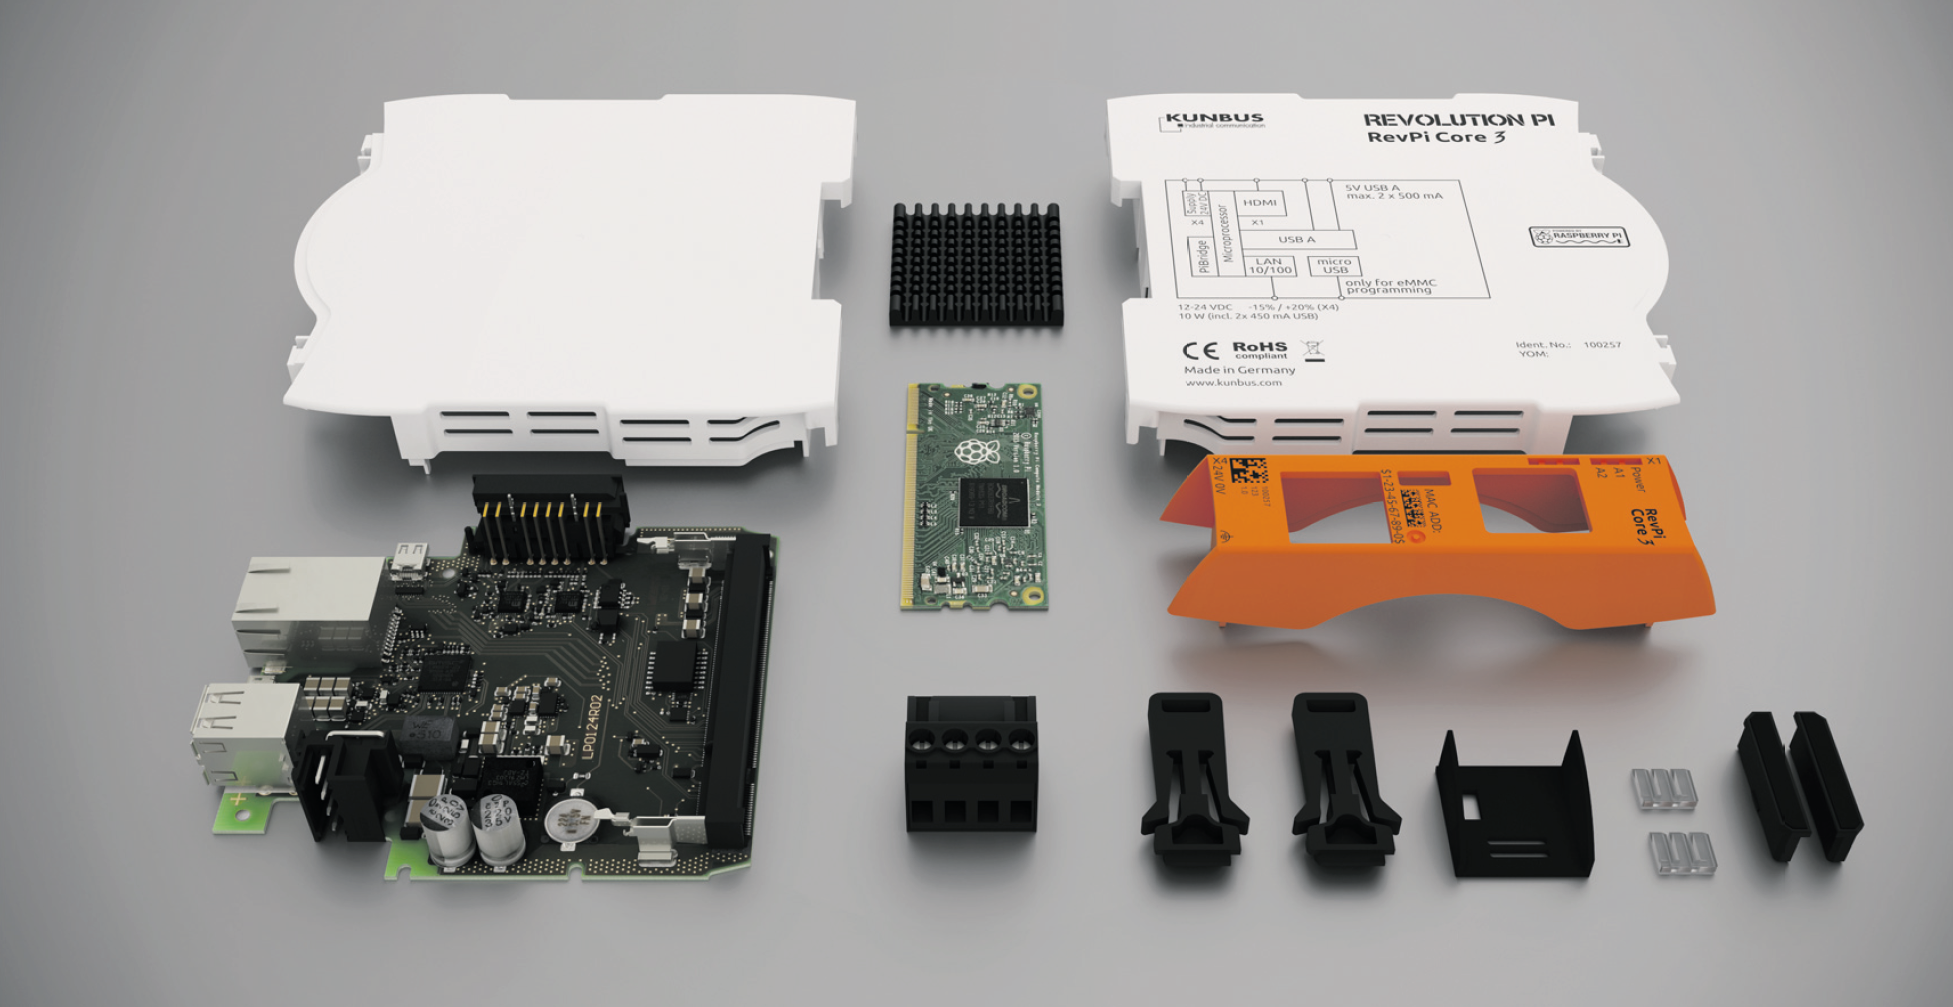
\includegraphics[width=0.85\textwidth]{doc/tex/images/revpi_teardown.png}
    \caption{Der RevPi Core 3 und seine Einzelkomponenten (Quelle: Kunbus)
      \label{fig:revpi-expl}}
\end{figure}

Spezifikationen des RevPi Core 3 \citep[Auswahl, vgl.][S. 1]{datasheet-revpi}:
\begin{itemize}
  \item{Prozessor: BCM2837}
  \item{Taktfrequenz 1,2 GHz}
  \item{Anzahl Prozessorkerne: 4}
  \item{Arbeitsspeicher: 1 GByte}
  \item{eMMC Flash Speicher: 4 GByte}
  \item{Betriebssystem: Angepasstes Raspbian mit RT-Patch}
  \item{RTC mit 24h Pufferung über wartungsfreien Kondensator}
  \item{Treiber / API: Kernel-Treiber schreibt zyklisch Prozessdaten in ein Prozessabbild, Zugriff auf Prozessabbild mittels ioctl-Anfragen oder über Linux-Dateisystem als API zu Fremdsoftware}
  \item{Kommunikationsanschlüsse: 2 x USB 2.0 A, 1 x Micro-USB, HDMI, Ethernet 10/100 Mbit/s}
  \item{Stromversorgung: min. 10,7 V, max. 28,8 V, maximal 10 Watt}
\end{itemize}

Kunbus stellt für den Revolution Pi ein auf Raspbian\footnote{Raspbian ist eine speziell 
für den Raspberry Pi angepasste Variante von Debian.} Stretch basierendes Betriebssystem bereit.
Verwendet wird der Kernel 4.9.76-rt60-v7+ in Verbindung mit dem SMP PREEMPT RT Patch.

\begin{figure}
    \centering
    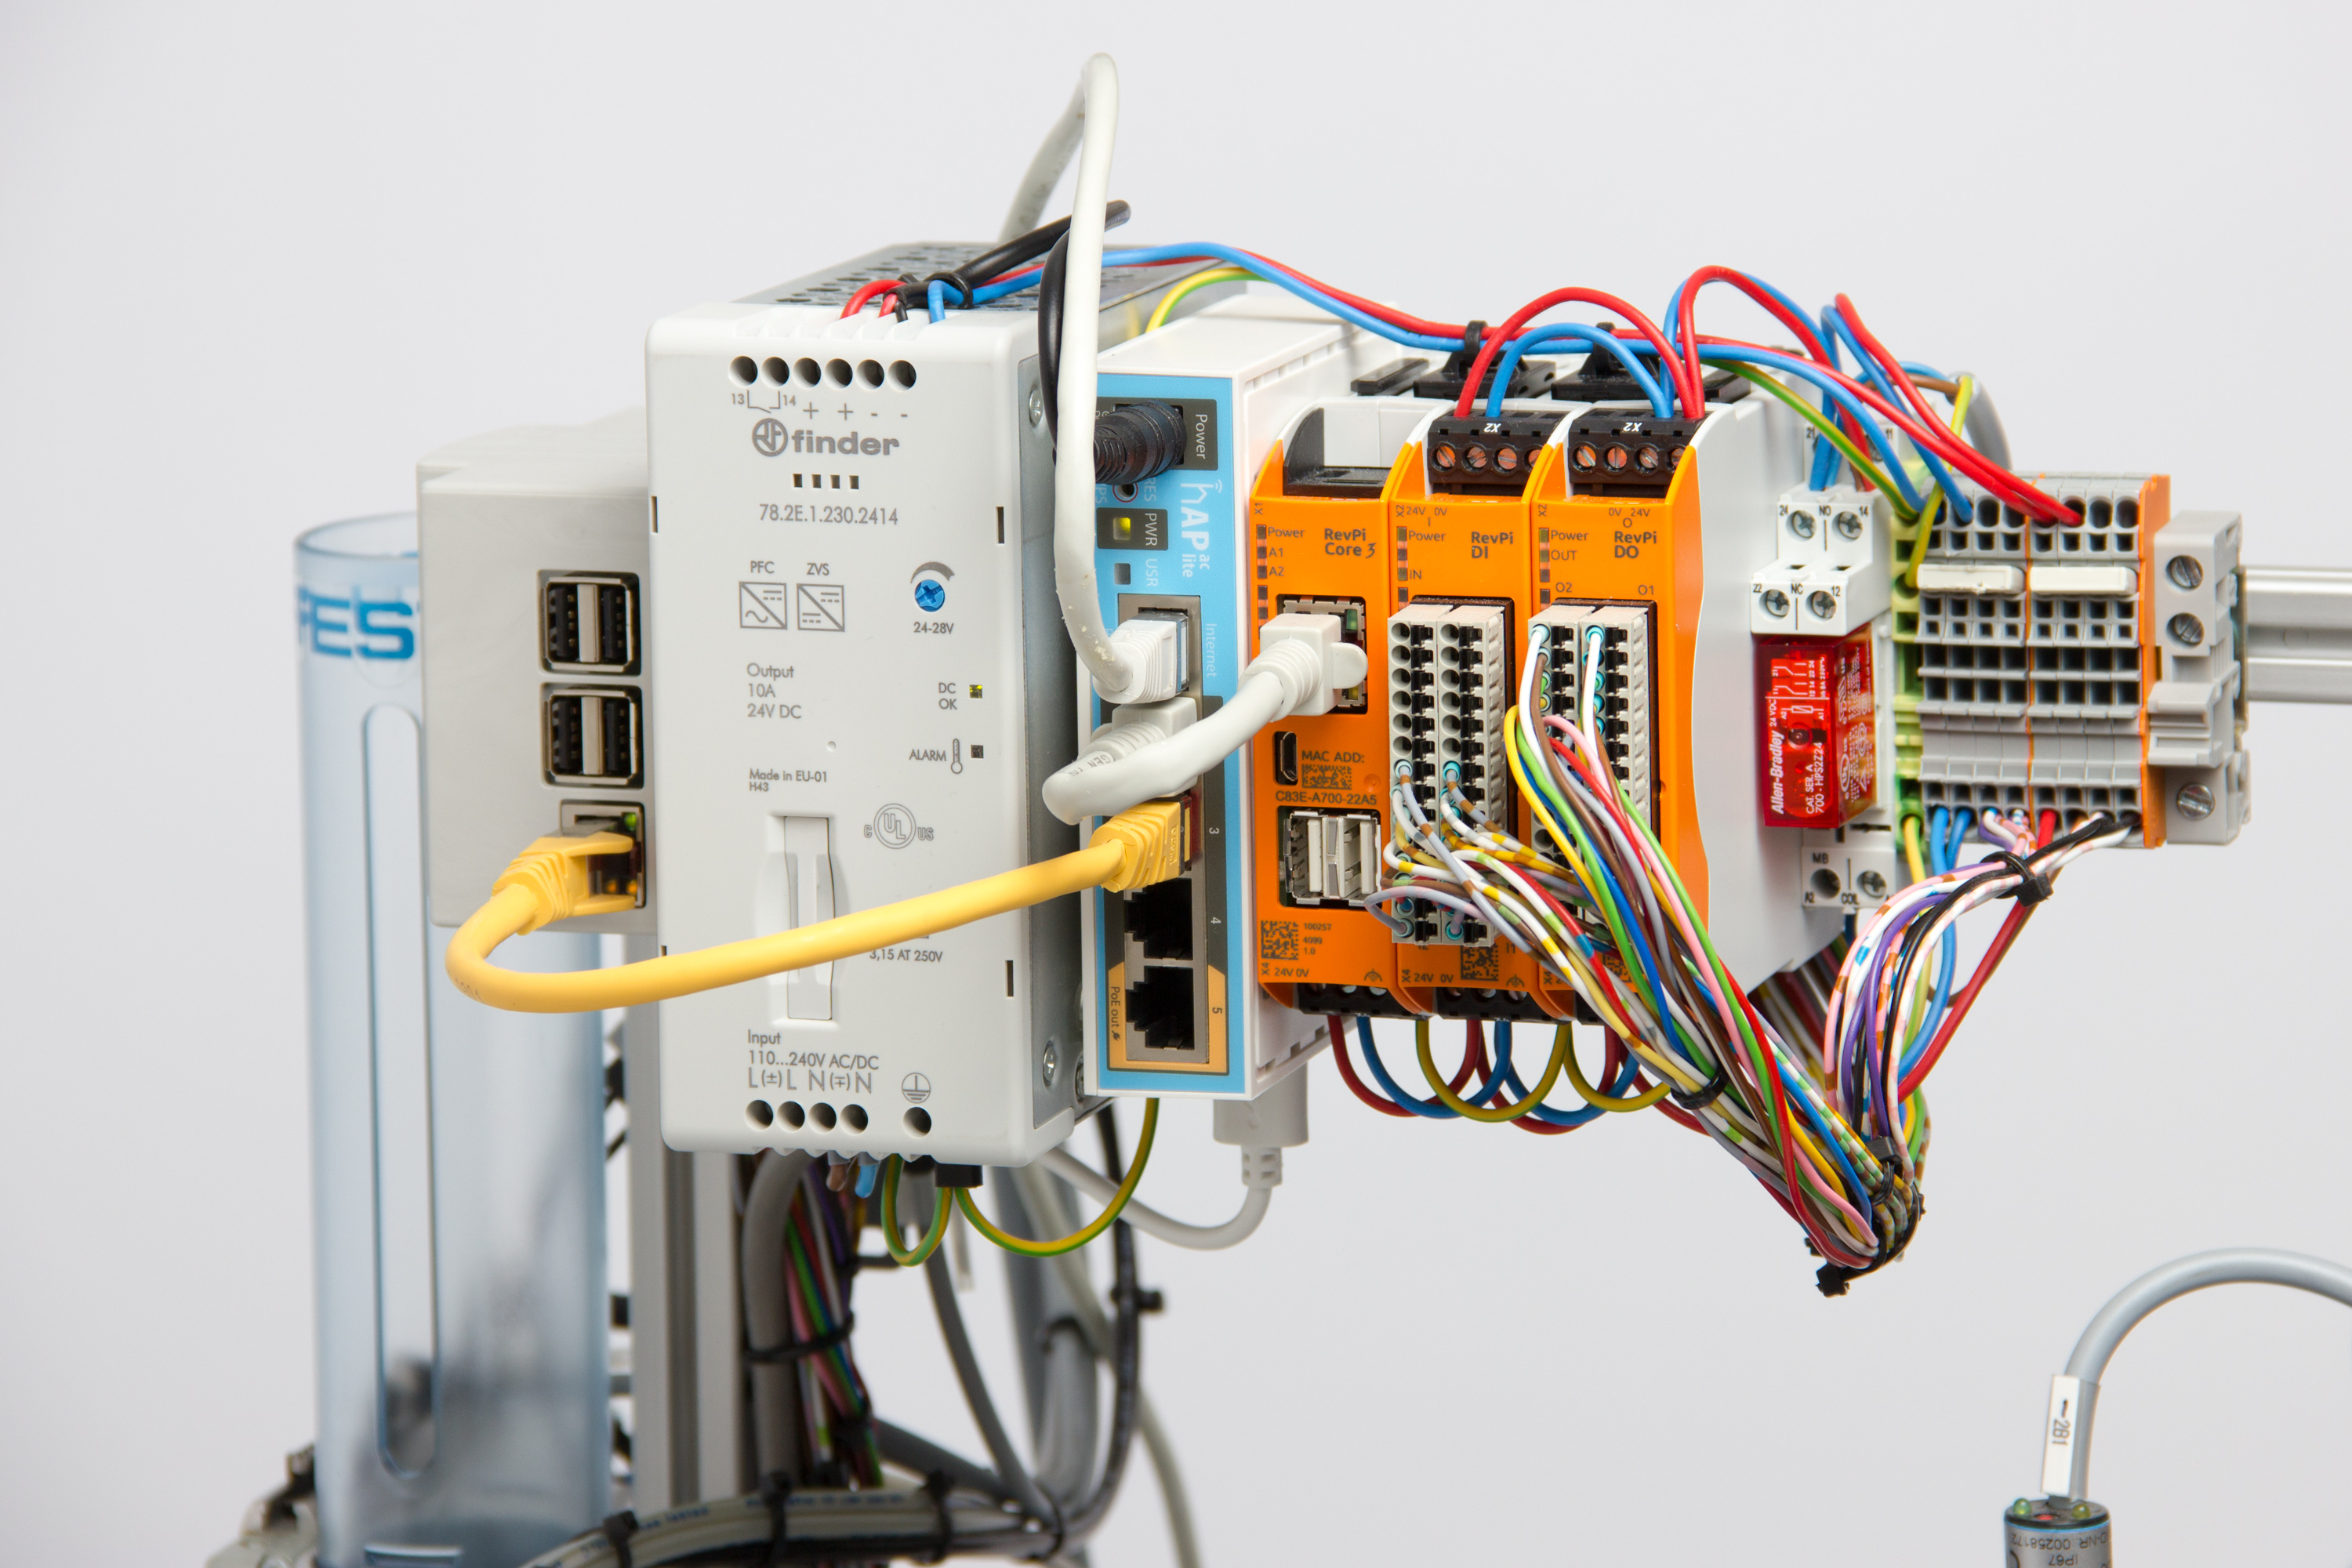
\includegraphics[trim={13cm 5cm 1cm 3cm}, clip, width=0.85\textwidth]{../photos/serverless_plc_img_8}
    \caption{Der Revolution Pi 3 mit digitalen IO-Modulen}
    \label{fig:rev-pi-io}
\end{figure}

Kunbus bietet neben dem sog. Core auch IO- und Gateway-Modulen zur Erweiterung der SPS an, siehe Bild~\ref{fig:rev-pi-io}.
Gateways dienen der Kommunikation mit externen Systemen oder Komponenten
über in der Automatisierungstechnik gängige Protokolle wie PROFIBUS oder EtherCAT. 
IO-Module erlauben die Überwachung und Steuerung von digitalen oder analogen Ein- und Ausgängen (IOs).

Kunbus deklariert die Hardware des Revolution Pi als Open-Source \citep[vgl.][S. 4]{flyer-revpi}. 
Die Schaltpläne des Revolution Pi, genauer die des RevPi Core 3 und der IO-Module, stehen auf der
Website\footnote{\label{downloads}\url{https://revolution.kunbus.com/tutorials/downloads/}} des Herstellers zum 
Download bereit. Eine Lizenz wird nicht angegeben.
Die Raspberry Pi Foundation stellt die Schaltpläne des Compute Modules des weiteren in ihrem Gitub-Repository 
zum Download bereit.

Sowohl die Raspberry Pi Foundation als auch die Kunbus GmbH pflegen aktiv ihre öffentlichen Repositories\footnote{\url{https://github.com/raspberrypi/} resp.~\url{https://github.com/RevolutionPi/}}
auf Github. 

% Kunbus konnte so einige Verbesserungen zum Linux Kernel 4.15 beitragen
% \footnote{siehe \url{https://revolution.kunbus.com/our-contribution-to-linux-4-15/}}.
% \todo{letzten Absatz evtl. weglassen? an sich nicht schlecht, passt aber irgendwie 
% nicht richtig zum Rest und stört den Lesefluss}

\subsubsection{Zugriff auf IO-Module%
        \label{sec:2-io}}
Der Zugriff auf die Ein- und Ausgänge der IO-Module erfolgt über einen RS485-Bus und einen in Form eines Kernel-Moduls bereitgestellten Treiber, genannt piControl. Der RS485-Bus ist über die serielle Schnittstelle des Compute Modules angebunden. 
piControl stellt ein Prozessabbild bereit, welches den physikalischen Zustand der Ein- und Ausgänge der IO-Module repräsentiert.
Das Prozessabbild wird, wie in der Automatisierungstechnik üblich, zyklisch aktualisiert. 
Die angestrebte Zykluszeit beträgt 5ms, kann jedoch je nach Anzahl der angeschlossenen Module auch größer sein. 
Kunbus garantiert bei drei IO-Modulen und zwei Gateway-Modulen eine Zykluszeit von 10 ms \citep[vgl.][]{web-revpi-dio}.
Die garantierte Zykluszeit ermöglicht die Umsetzung von Anwendungen mit harten Echtzeit-Anforderungen.

Fremdanwendungen können über eine Applikationsschnittstelle (API) auf das Prozessabbild zugreifen. 
Hierzu stellt das Kernel-Modul piControl sowohl \lstinline{seek}, \lstinline{read} und \lstinline{write} Methoden zur verfügung, wie auch die Möglichkeit mittels \lstinline{ioctl}-Anfragen gezielt auf einzelne Variablen des Prozessabbildes zuzugreifen.
In der englischsprachigen Wikipedia werden ioctl-Aufrufe wie folgt beschrieben:

\glqq{}The kernel is designed to be extensible, and may accept an extra module called a device driver which runs in kernel space and can directly address the device. An ioctl interface is a single system call by which userspace may communicate with device drivers. [...] The basic kernel can thus allow the userspace to access a device driver without knowing anything about the facilities supported by the device, and without needing an unmanageably large collection of system calls.

[...] ioctl calls provide a convenient way to bridge userspace code to kernel extensions. Kernel extensions can provide a location in the filesystem that can be opened by name, through which an arbitrary number of ioctl calls can be dispatched, allowing the extension to be programmed without adding system calls to the operating system.\grqq{}\citep[vgl.][]{web-wiki-ioctl}

Der Quellcode von piControl steht unter der GNU General Public License Version 2 (GNU GPLv2) und ist 
auf Github verfügbar\footnote{\url{https://github.com/RevolutionPi/piControl}}. Als Einstieg in die 
Entwicklung eigener Steuerungsprogramme liefert Kunbus das C-Programm piTest mit. Dieses verwendet 
piControl und erlaubt dem Nutzer über Kommandozeilen-Parameter die angeschlossenen IO-Module zu steuern.

\begin{figure}[h]
    \centering
    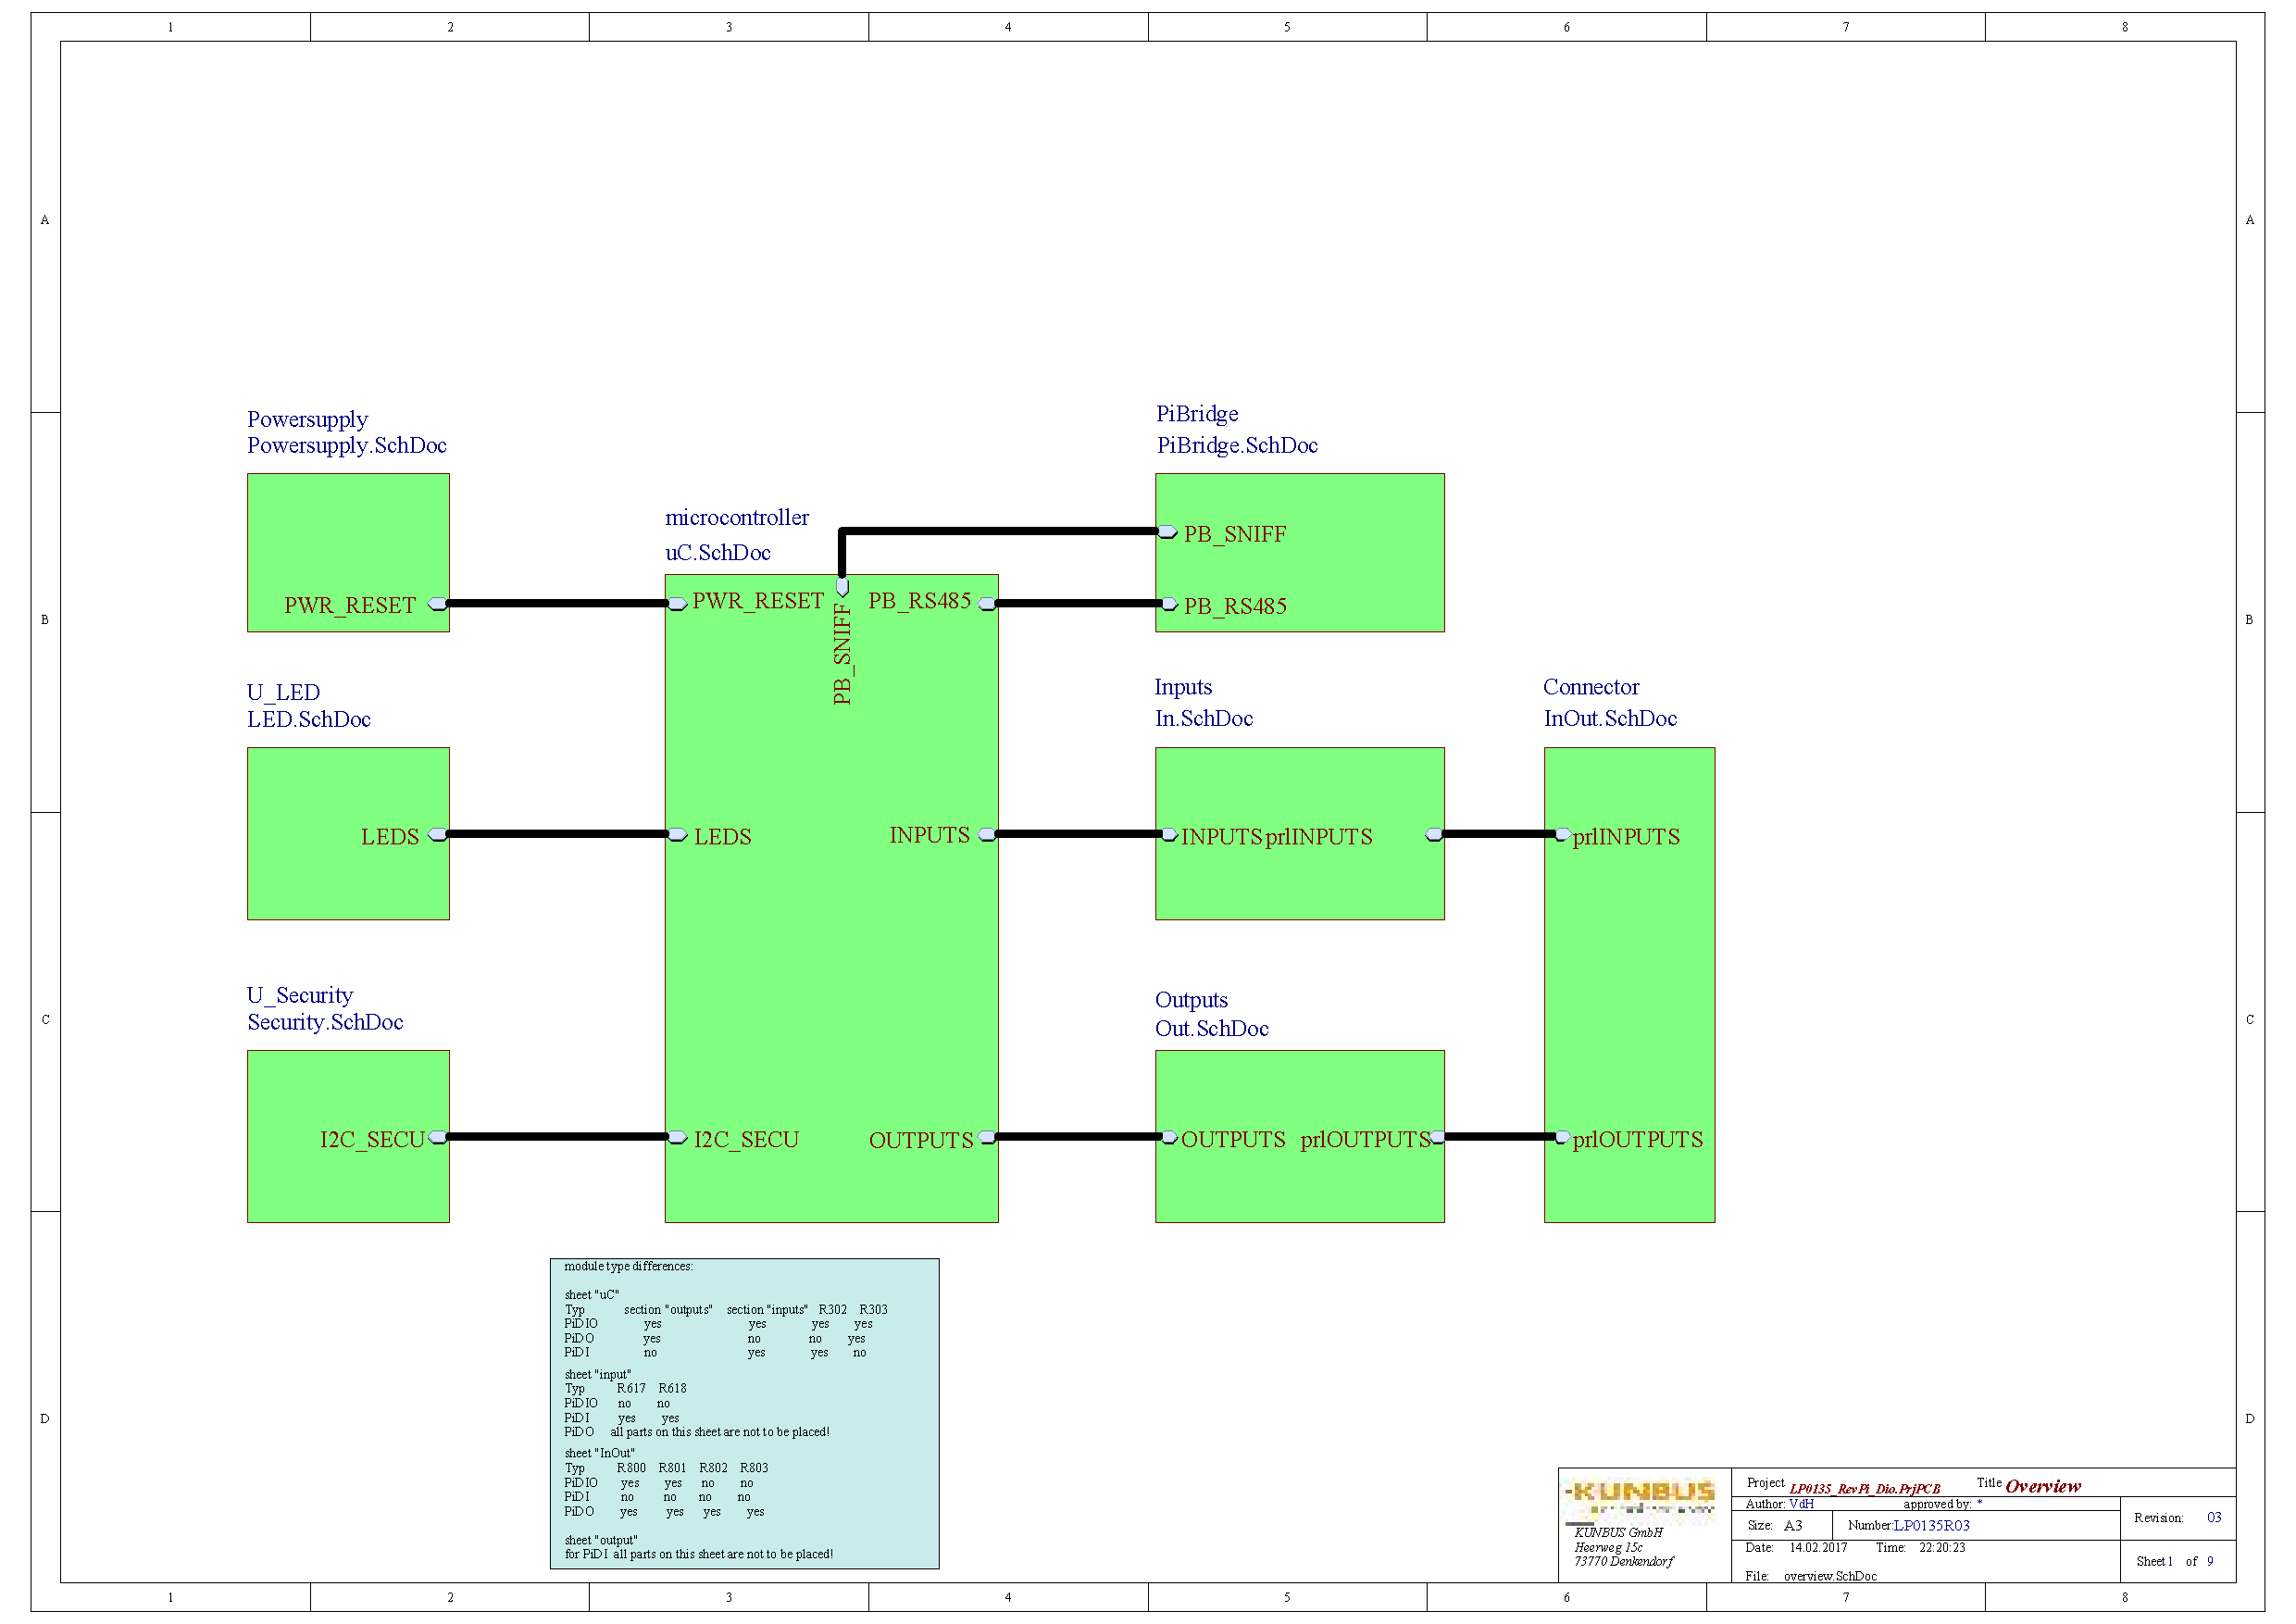
\includegraphics[trim={4cm 7cm 10.5cm 7.3cm}, clip, width=\textwidth]{literature/SchematicPrintsRevPi-DIO}
    \caption{Schematische Darstellung eines DIO-Moduls (Quelle: Kunbus\textsuperscript{\ref{downloads}})
      \label{fig:dio}}
\end{figure}

Jedes der IO-Module stellt ein eigenständiges eingebettetes System dar. Es verfügt
über einen Microcontroller, welcher die IOs bereitstellt und über einen RS485-Bus
mit dem Revolution Pi kommuniziert (siehe Bild~\ref{fig:dio}). 
Kunbus stellt exemplarisch den Quellcode eines DIO-Moduls unter der MIT Lizenz zur
Verfügung\footnote{\url{https://github.com/RevolutionPi/IODeviceExample}}. 


\subsection{Echtzeit und Multitasking unter Linux -- preemptRT und posix%
     \label{sec:2-echtzeit}}
     
Moderne Betriebssysteme realisieren Multitasking i.d.R.\,in Form des präemptiven Multitasking. 
Der Kernel verfügt über einen sog. Scheduler. Dieser priorisiert alle Prozesse und weist ihnen 
Rechenzeit in sog. Time Slots zu. Die Größe der Zeitfenster sowie die Ausführungsreihenfolge 
ist von der Priorität eines Prozesses abhängig. Besonders an einem präemptiven im Gegensatz zu einem kooperativen Scheduler ist dessen Fähigkeit, Tasks während ihrer Ausführung zu unterbrechen bzw. zu pausieren, wenn diese eine bestimmte Dauer überschreiten oder ein höher priorisierter Prozess (bspw. ausgelöst durch einen Interrupt oder durch eine inhärente Periodizität) Rechenleistung benötigt.

Eine Sonderform des präemptiven Multitasking ist das präemptible Multitasking. Hierbei werden auch Teile 
des Kernels als Threads durch den Scheduler ausgeführt. Dieser ist somit in der Lage, auch Prozesse des Kernels
zu unterbrechen, wenn andere Anwendungen Prozessorzeit oder Zugriff auf andere Systemressourcen benötigen
\citep[vgl.][]{web-wiki-praempt}.
     
Der Linux-Kernel implementiert unterschiedliche Präemptions-Modelle \citep[vgl.][/preemption\_models]{web-linuxwiki-basics}:

\begin{itemize}
  \item No Forced Preemption (server):
  Ausgelegt auf maximal möglichen Durchsatz, lediglich Interrupts und
  System-Call-Returns bewirken Präemption.

  \item Voluntary Kernel Preemption (Desktop):
  Neben den implizit bevorrechtigten Interrupts und System-Call-Returns gibt es
  in diesem Modell weitere Abschnitte des Kernels in welchen Preämption explizit
  gestattet ist.

  \item Preemptible Kernel (Low-Latency Desktop):
  In diesem Modell ist der gesamte Kernel, mit Ausnahme sog.~kritischer Abschnitte
  präemptible. Nach jedem kritischen Abschnitt gibt es einen impliziten Präemptions-Punkt.

  \item Preemptible Kernel (Basic RT):
  Dieses Modell ist dem zuvor genannten sehr ähnlich, hier sind jedoch alle Interrupt-Handler
  als eigenständige Threads ausgeführt.

  \item Fully Preemptible Kernel (RT):
  Wie auch bei den beiden zuvor genannten Modellen ist hier der gesamte Kernel
  präemtible. Die Anzahl und Dauer der nicht-präemtiblen kritischen Abschnitte
  ist auf ein notwendiges Minimum beschränkt. Alle Interrupt-Handler sind als
  eigenständige Threads ausgeführt, Spinlocks durch Sleeping-Spinlocks und Mutexe
  durch sog.~RT-Mutexe ersetzt.

\end{itemize}

Lediglich ein präemtibler Kernel kann hartes Echtzeit-Verhalten realisieren, 
da nur hier eine maximale Antwortzeit garantiert werden kann.
Viele Prozesse in der Automatisierungstechnik erfordern harte Echtzeit. 
Eine verspätete Antwort auf eine Anfrage, 
wie etwa das Signal eines Lagenendschalters oder eines Notausschalters kann hier nicht nur über
den Erfolg eines Prozesses, sondern auch über das Leben der daran beteiligten Mitarbeiter entscheiden.
Für weiterführende Erklärungen bzgl.\,Echtzeit, Mutexen und 
Spinlocks sei an dieser Stelle auf die Vorlesung verwiesen~\citep{script-peter}.


\subsubsection{preemptRT%
        \label{sec:2-preemptRT}}

Der Kernel des auf dem Revolution Pi installierten Raspbian mit PREEMP\_RT Patch fällt 
in die Kategorie des \glqq{}Fully Preemptible Kernels\grqq{} (siehe Abschnitt \ref{sec:2-echtzeit}).
Das zugrunde liegende Prinzip lässt sich wie folgt formulieren: Nur Code, welcher absolut nicht-präemtible sein darf, ist es
gestattet nicht-präemtible zu sein. Ziel ist folglich, die Menge des nicht-präemtiblen 
Codes im Linux-Kernel auf das absolut notwendige Minimum zu reduzieren.

Dies wird durch Verwendung folgender Mechanismen erreicht~\citep[vgl.][]{web-linuxwiki-details}:

\begin{itemize}
  \item Hochauflösende Timer
  \item Sleeping Spinlocks
  \item Threaded Interrupt Handlers
  \item rt\_mutex
  \item RCU
\end{itemize}

Diese Mechanismen sind bspw. im Linux-Wiki\footnote{siehe \url{https://wiki.linuxfoundation.org/realtime/documentation/technical_details}} ausführlich beschrieben.

\subsubsection{POSIX%
        \label{sec:2-posix}}
Das Portable Operating System Interface (POSIX) bezeichnet eine Sammlung von Standards, 
welche auf dem Unix-System basieren, jedoch nicht auf dieses beschränkt sind.

Der Wechsel zwischen verschiedenen Unix-Distributionen brachte oft Kompatibilitätsprobleme mit sich. 
Dieser Mangel an Portabilität erschwerte Benutzern und Entwicklern die Verwendung bzw. Bereitstellung 
von Software auf unterschiedlichen Systemen. 
Das Institut für Elektrotechnik und Elektronik (IEEE) begann 1984 mit der Entwicklung des Unix-Standards.
Sie entwickelten das, was heute als Single UNIX Specification bekannt ist und allgemein als POSIX bezeichnet wird~\citep[vgl.][]{web-debianwiki-posix}.
Das Konsortium \glqq{}The Open Group\grqq{} überwacht die weitere Entwicklung dieses Standards.
Ferner stellt es einen Teil der POSIX-Spezifikation frei zur Verfügung~\citep[vgl.][]{web-opengroup-posix}.

Die aktuelle Version POSIX.1-2017 ist verfügbar als IEEE Standard 1003.1-2017 sowie in Form der \glqq{}The Open Group Technical Standard Base Specifications\grqq{}, Ausgabe 7. POSIX.1-2017 definiert eine Standard-Betriebssystemschnittstelle und -umgebung, einschließlich eines Befehlsinterpreters (auch Shell genannt) und gängiger Dienstprogramme zur Unterstützung der Portabilität von Anwendungen auf Quellcode-Ebene. POSIX.1-2017 ist sowohl für Anwendungsentwickler als auch für Systemimplementierer gedacht und umfasst vier Hauptkomponenten \citep[vgl.][]{web-opengroup-overview}:
\begin{itemize}
    \item Basisdefinitionen:\\
          Allgemeine Begriffe, Konzepte und Schnittstellen einschließlich Hilfskonventionen und C-Headern
          
    \item Systemschnittstellen:\\
          Definitionen für Systemdienstfunktionen und Unterprogramme, C-spezifische Systemdienste, Portabilität
        
    \item Shell und Dienstprogramme:\\
          Definitionen für eine Schnittstelle zur Befehlsinterpretation von Diensten und gängige Hilfsprogramme
    
    \item Begründungen und Historie
\end{itemize}

Debian basiert auf Linux und verwendet den Linux-Kernel. Linux ist zu großen Teilen POSIX-kompatibel. Debian ist jedoch nicht POSIX-zertifiziert, da diese Zertifizierung mit hohen Kosten verbunden ist\citep[vgl.][Kapitel 4.4.]{web-debian-faq}.

Beide Kernkomponenten des in dieser Arbeit vorgestellten Projektes nutzen Komponenten von Linux, 
welche an den POSIX-Standard angelehnt sind: open62541 verwendet u.a.\,POSIX-Threads und
Mutexe~\citep[vgl.][pthread.h]{web-opengroup-pthread}, piControl nutzt POSIX-Semaphoren
\citep[vgl.][semaphore.h]{web-opengroup-semaphore}. 


\subsection{OPC-UA und open62541%
     \label{sec:2-opc}}
In diesem Abschnitt sollen Möglichkeiten des Datenaustausch zwischen Komponenten der
Automatisierungstechnik vorgestellt werden. OPC-UA stellt einen offenen, IP-basierten Kommunikationsstandard
für Sensoren und Steuerungen dar. open62541 ist eine freie Client- sowie Server-Implementierung dieses
Standards, geschrieben in C.


\subsubsection{OPC UA%
        \label{sec:2-opcua}}

Open Platform Communications (OPC) ist eine Familie von Standards zur herstellerunabhängigen
Kommunikation von Maschinen (M2M) in der Automatisierungstechnik. Die sog. OPC Task Force, zu deren
Mitgliedern verschiedene etablierte Firmen der Automatisierungsindustrie gehören, veröffentlichte
die OPC Specification Version 1.0 im August 1996.
Motiviert ist dieser offene Standard durch die Erkenntniss, dass die Anpassung der
zahlreichen Herstellerstandards an individuelle Infrastrukturen und Anlagen einen
großen Mehraufwand verursachen.
Die Wikipedia beschreibt das Anwendungsgebiet für OPC wie folgt \citep[vgl.][]{web-wiki-opc}:

\glqq{}OPC wird dort eingesetzt, wo Sensoren, Regler und Steuerungen verschiedener Hersteller
ein gemeinsames Netzwerk bilden. Ohne OPC benötigten zwei Geräte zum Datenaustausch
genaue Kenntnis über die Kommunikationsmöglichkeiten des Gegenübers. Erweiterungen
und Austausch gestalten sich entsprechend schwierig. Mit OPC genügt es, für jedes
Gerät genau einmal einen OPC-konformen Treiber zu schreiben. Idealerweise wird
dieser bereits vom Hersteller zur Verfügung gestellt. Ein OPC-Treiber lässt sich
ohne großen Anpassungsaufwand in beliebig große Steuer- und Überwachungssysteme
integrieren.

OPC unterteilt sich in verschiedene Unterstandards, die für den jeweiligen Anwendungsfall
unabhängig voneinander implementiert werden können. OPC lässt sich damit verwenden
für Echtzeitdaten (Überwachung), Datenarchivierung, Alarm-Meldungen und neuerdings
auch direkt zur Steuerung (Befehlsübermittlung).\grqq{}

OPC basiert in der ursprünglichen Spezifikation (auch als OPC DA bezeichnet) auf Microsofts DCOM-Spezifikation.
DCOM macht Funktionen und Objekte einer Anwendung anderen Anwendungen im Netzwerk
zugänglich. Der OPC-Standard definiert entsprechende DCOM-Objekte um mit anderen
OPC-Anwendungen Daten austauschen zu können. Die Verwendung von DCOM bindet Anwender
jedoch an Betriebssysteme von Microsoft. 

\begin{figure}
    \centering
    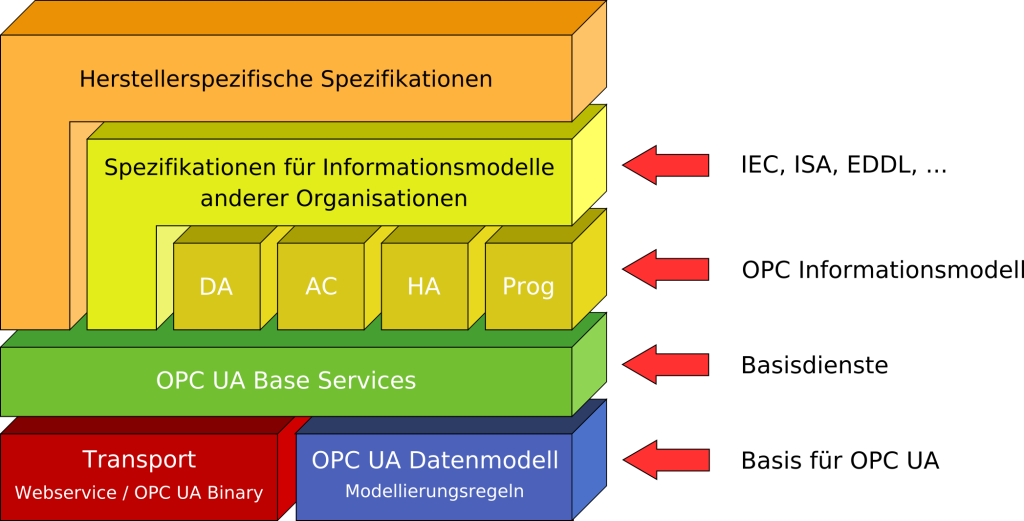
\includegraphics[width=0.85\textwidth]{images/UA_Architecture_1024.png}
    \caption{Die OPC Unified Architecture. Grafik von Gerhard Gappmeier - ascolab GmbH, CC BY-SA 3.0}
    \label{fig:opc-unified-architecture}
\end{figure}
% Evtl Grafik: Von Gerhard Gappmeier - ascolab GmbH, CC BY-SA 3.0, https://de.wikipedia.org/w/index.php?curid=1892069

Die ursprüngliche OPC Spezifikation wurde 2006 durch die Entwicklung der 
OPC Unified Architecture (OPC UA) überholt. 
Diese zeichnet sich durch eine Service-orientierte Architektur (SOA) aus, deren Struktur
aus mehreren Schichten besteht, siehe Abbilung~\ref{fig:opc-unified-architecture}. 
Über der untersten Schicht, dem Betriebssystem des Servers, verbindet eine Portabilitäts-Schicht 
den sog.\, UA ANSI C Stack mit einer API. Diese API kann bspw.\,in C++ geschrieben sein, 
und erlaubt die Anbindung der obersten Schicht, der Anwendungsschicht~\citep[vgl.][]{web-spec-opc}.
OPC UA setzt auf einem eigenen Kommunikationsstack auf; die Verwendung von DCOM
und damit die Bindung an Microsoft wurden aufgelöst.

Neben Architektur und Kommunikationsschnittstellen wird in der OPC Spezifikation auch ein 
Informationsmodell definiert. Die deutschsprachige Wikipedia beschreibt dieses wie folgt: 

\glqq{}Das OPC[-UA]-Informationsmodell ist nicht mehr nur eine Hierarchie aus Ordnern, Items
und Properties. Es ist ein sogenanntes Full-Mesh-Network aus Nodes, mit dem neben
den Nutzdaten eines Nodes auch Meta- und Diagnoseinformationen repräsentiert werden. [...]
Ein Node ähnelt einem Objekt aus der objektorientierten Programmierung. Ein Node
kann Attribute besitzen, die gelesen werden können. Es ist möglich Methoden zu definieren und aufzurufen. [...]
Weiterhin werden Events unterstützt, die versendet werden können
(AE (Alarms \& Events), DA DataChange), um bestimmte Informationen zwischen Geräten
auszutauschen. Ein Event besitzt unter anderem einen Empfangszeitpunkt, eine Nachricht
und einen Schweregrad. Die o.\,g. Nodes werden sowohl für die Nutzdaten als auch
alle anderen Arten von Metadaten verwendet. Der damit modellierte OPC-Adressraum
beinhaltet nun auch ein Typmodell, mit dem sämtliche Datentypen spezifiziert werden.\grqq{}


\subsubsection{open62541%
        \label{sec:2-open62541}}
open62541 ist eine offene und freie Implementierung von OPC UA. 
Die in C geschriebene Bibliothek stellt eine beständig zunehmende Anzahl der im OPC UA Standard definierten
Funktionen bereit. Sie kann sowohl zur Erstellung von OPC-Servern als auch von -Clients
genutzt werden. Ergänzend zu der unter der Mozilla Public License v2.0 lizensierten
Bibliothek stellt das open62541 Projekt auch Beispielprogramme unter einer CC0 Lizenz
zur Verfügung.
Zu den Unterstützern des Projektes zählen u.a.\, die RWTH Aachen, das Frauenhofer IOSB sowie die TU Dresden.

Die Bibliothek eignet sich auch für die Entwicklung auf eingebetteten Systemen und
Microcontrollern. Die Größe einer Server-Binary kann weniger als 100kB betragen.

Folgende Auswahl an Eigenschaften und Funktionen zeichnet die in dieser Arbeit verwendete
Version 0.3 von open62541 aus:
\begin{itemize}
  \item Kommunikationionsstack
  \begin{itemize}
      \item OPC UA Binär-Protokoll (HTTP oder SOAP werden gegenwärtig nicht unterstützt)
      \item Austauschbare Netzwerk-Schicht, welche die Verwendung eigener Netzwerk-APIs
      erlaubt.
      \item Verschlüsselte Kommunikationion
      \item Asynchrone Dienst-Anfragen im Client
  \end{itemize}
  \item Informationsmodell
  \begin{itemize}
    \item Unterstützung aller OPC UA Node-Typen, inkl.~Methoden
    \item Hinzufügen und Entfernen von Nodes und Referenzen zur Laufzeit.
    \item Vererbung und Instanziierung von Objekt- und Variablentypen
    \item Zugriffskontrolle auch für einzelne Nodes
  \end{itemize}
  \item Subscriptions
  \begin{itemize}
    \item Erlaubt die Überwachung (subscriptions / monitoreditems)
    \item Sehr geringer Ressourcenbedarf pro überwachtem Wert
  \end{itemize}
  \item Code-Generierung auf XML-Basis
  \begin{itemize}
    \item Erlaubt die Erstellung von Datentypen
    \item Erlaubt die Generierung des serverseitigen Informationsmodells
  \end{itemize}
\end{itemize}

Weiterführende Informationen und Code-Beispiele bietet die ausführliche Dokumentation des Projektes~\citep[siehe]{web-open62541} sowie der kommentierte Quelltext.

% % % Imports nur für Referenzenauflösung während des Schreibens! Vorm Kompilieren auskommentieren!
% \bibliography{0_hauptdatei}
% \input{1_einleitung}
% \input{2_grundlagen}
% \input{3_konzeption}
% \input{4_implementierung}
% \input{5_tests}
% \input{6_zusammenfassung}
% \input{anhang}
% % Ende Imports

\section{Systemkonzept%
  \label{sec:3-konzeption}}
Auf Basis der in Abschnitt [...] vorgestellten Möglichkeiten folgt nun die Ausarbeitung eines Konzepts.

\subsection{Anbindung der IO an den OPC-Server%
     \label{sec:3-anbindung}}

\subsection{Integration des OPC-Servers in das System%
     \label{sec:3-integration}}

% % % Imports nur für Referenzenauflösung während des Schreibens! Vorm Kompilieren auskommentieren!
% \bibliography{0_hauptdatei}
% \input{1_einleitung}
% \input{2_grundlagen}
% \input{3_konzeption}
% \input{4_implementierung}
% \input{5_tests}
% \input{6_zusammenfassung}
% \input{anhang}
% % Ende Imports

\section{Implementierung%
  \label{sec:4-implementierung}}
Das folgende Kapitel stellt in Auszügen die Implementierung des OPC-Servers sowie die Anbindung an die IO-Module
der SPS dar. Der Schwerpunkt liegt hierbei auf der Funktionsweise des piControl-Treibers und dessen Integration in das Projekt. Abschnitt~\ref{sec:4-picontrol} erklärt die zum Schreibens eines Bits verwendeten Funktionsaufrufe.
Zuvor soll jedoch in Abschnitt~\ref{sec:4-open62541} der Teil des OPC-Servers vorgestellt werden, welcher auf besagten Treiber zugreift. 

\subsection{Implementierung des OPC-Servers%
     \label{sec:4-open62541}}
Wie im vorangegangenen Abschnitt~\ref{sec:3-integration} begründet, soll die Verknüpfung zwischen dem Prozessabbild der SPS und den auf dem OPC-Server bereitgestellten Werten über sog.\,Datenquellen erfolgen. Hierzu ist zunächst eine Callback-Methode zu implementieren, welche bei einem Lese- oder Schreibzugriff auf eine Variable aufgerufen wird. Die Verknüpfung zwischen Callback-Methode und Variable muss manuell erfolgen.

\begin{lstlisting}[language={c},firstnumber=237,caption={Auszug der Methode \lstinline{linkDataSourceVariable} in \lstinline{variables.c}\label{lst:4-linkDataSourceVariable}}]
extern UA_StatusCode
 linkDataSourceVariable(UA_Server *server, UA_NodeId nodeId) {
     bool readonly = false;
     UA_DataSource dataSourceVariable;
     UA_StatusCode rc; |>\setcounter{lstnumber}{254}<|

     dataSourceVariable.read = readDataSourceVariable;
     if (!readonly)
        dataSourceVariable.write = writeDataSourceVariable;
     else
        dataSourceVariable.write = writeReadonlyDataSourceVariable;

     return UA_Server_setVariableNode_dataSource(server, nodeId, dataSourceVariable);
 }
\end{lstlisting}

\begin{figure}[h]
    \centering
    \includegraphics[width=0.42\textwidth]{doc/img/OPC_RevPiDO.pdf}
    \caption{Auszug des verwendeten Nodesets, hier Digitalausgang 1 des Versuchsaufbaus
      \label{fig:opc-do}}
\end{figure}

Die in Listing~\ref{lst:4-linkDataSourceVariable} abgebildete Methode \lstinline{linkDataSourceVariable()} erzeugt ein Struct vom Typ \lstinline{UA_DataSource}. In diesem werden dem Lesen und Schreiben einer OPC-Variablen entsprechende Callback-Methoden zugewiesen. Die Verknüpfung einer OPC-Variable, genauer ihrer NodeId, mit der zuvor definierten Datenquelle erfolgt über die von open62541 bereitgestellte Methode \lstinline{UA_Server_setVariableNode_dataSource()}. Vor dem Lesen und nach dem Schreiben dieser Variable werden von nun an die entsprechenden Callbacks aufgerufen.
     
\begin{lstlisting}[language={c},firstnumber=168,caption={Auszug des Callbacks \lstinline{writeDataSourceVariable} in \lstinline{variables.c}\label{lst:4-writeDataSourceVariable}}]  
extern UA_StatusCode
 writeDataSourceVariable(UA_Server *server,
            const UA_NodeId *sessionId, void *sessionContext,
            const UA_NodeId *nodeId, void *nodeContext,
            const UA_NumericRange *range, const UA_DataValue *dataValue) {

    UA_StatusCode retval  = UA_STATUSCODE_GOOD;
    UA_NodeId *nameNodeId = UA_malloc(sizeof(UA_NodeId));
    UA_QualifiedName nameQN = UA_QUALIFIEDNAME(1, "Name");
    UA_Variant nameVar;
    UA_Boolean bit;

    retval |= findSiblingByBrowsename(server, nodeId, &nameQN, nameNodeId);
    retval |= UA_Server_readValue(server, *nameNodeId, &nameVar);
    retval |= UA_Boolean_copy(dataValue->value.data, &bit);

    |>\tikzmarkin[set border color=martinired]{writeIO}<|PI_writeSingleIO(String_fromUA_String(nameVar.data), &bit, false);                                                 |>\tikzmarkend{writeIO}<|

    free(nameNodeId);
    return retval;
 }
\end{lstlisting}

Listing~\ref{lst:4-writeDataSourceVariable} zeigt die Callback-Methode, welche nach dem Schreiben einer Variablen auf dem OPC-Server aufgerufen wird.
Dieser Methode wird neben der NodeId der mit ihr verknüpften Variablen auch der Wert dieser in Form eines Zeigers auf ein Struct vom Typ \lstinline{UA_DataValue} übergeben.

Die Gestaltung des hier verwendeten Nodesets sieht vor, dass in einer OPC-Variablen \lstinline{"Name"} der Bezeichner des zu schreibenden Digitalausgangs hinterlegt ist, siehe Abbildung~\ref{fig:opc-do}. Dies erlaubt eine Rekonfiguration der Ein- und Ausgänge der SPS ohne Änderungen im Programmcode des OPC-Servers vornehmen zu müssen.
Es ist daher erforderlich, nach jedem Schreiben einer mit einem Digitalausgang verknüpften Variablen, hier \lstinline{"Value"}, dessen Bezeichner \lstinline{"Name"} abzufragen. 
Dies geschieht in den Zeilen 180 und 181.
Anschließend wird dieser Bezeichner sowie der zu schreibende Wert der Methode \lstinline{PI_writeSingleIO()} übergeben, welche wiederum die Interaktion mit piControl übernimmt (vgl. Abschnitt \ref{sec:4-picontrol}).
 
\subsection{Integration von piControl%
     \label{sec:4-picontrol}}
In Abschnitt~\ref{sec:2-io} wurde die Anbindung der IO-Module des Revolution Pi sowie die Funktionsweise von piControl aus Anwendersicht beschrieben. Die verfügbare Literatur beschränkt sich auch auf lediglich diese Sicht; eine weiterführende Dokumentation für Entwickler gibt es, neben der in Abschnitt~\ref{sec:3-anbindung} vorgestellten Manpage, nicht. 
In diesem Abschnitt soll daher der Quellcode von piControl sowie dessen Verwendung im Projekt genauer betrachtet werden.
Hierzu wird exemplarisch die in Abschnitt~\ref{sec:4-open62541} eingeführte Methode \lstinline{PI_writeSingleIO()} untersucht.
Diese Methode ermöglicht das Setzen eines einzelnen Bits im Prozessabbild der SPS, und damit das Schalten eines digitalen Ausgangs auf einem IO-Modul.
Die äquivalente Methode \lstinline{int piControlGetBitValue(SPIValue *pSpiValue)} zum Lesen eines Bits bzw. Eingangs funktioniert analog und soll daher an dieser Stelle nicht dediziert erörtert werden.

\begin{lstlisting}[language={c},firstnumber=97,
                   caption={Setzen eines phsikalischen, digitalen Ausgangs in \lstinline{revpi.c}
                   \label{lst:4-PI_writeSingleIO}}]
extern void PI_writeSingleIO(char *pszVariableName, bool *bit, bool verbose)
{
	int rc;
	SPIVariable sPiVariable;
	SPIValue sPIValue;

	strncpy(sPiVariable.strVarName, pszVariableName, sizeof(sPiVariable.strVarName));
	rc = piControlGetVariableInfo(&sPiVariable);
	if (rc < 0) {
		printf("Cannot find variable '%s'\n", pszVariableName);
		return;
	}

		sPIValue.i16uAddress = sPiVariable.i16uAddress;
		sPIValue.i8uBit = sPiVariable.i8uBit;
		sPIValue.i8uValue = *bit;
		rc = |>\tikzmarkin[set border color=martinired]{setBitValue}<|piControlSetBitValue(&sPIValue)|>\tikzmarkend{setBitValue}<|;
		if (rc < 0)
			printf("Set bit error %s\n", getWriteError(rc));
		else if (verbose)
			printf("Set bit %d on byte at offset %d. Value %d\n", sPIValue.i8uBit, sPIValue.i16uAddress,
			       sPIValue.i8uValue);
}
\end{lstlisting}

Der Programmcode in Listing~\ref{lst:4-PI_writeSingleIO} ist Teil des implementierten OPC-Servers. In diesem wird auf zwei Funktionen des piControl-Treibers zugegriffen. 
Beiden Methoden wird als Argument ein Zeiger auf ein Struct vom Typ \lstinline{SPIValue} übergeben. Der im Struct abgelegte Name wird mittels \lstinline{piControlGetVariableInfo(&sPIValue)} zu einer Adresse im Prozessabbild aufgelöst. Diese wird in \lstinline{sPIValue.i16uAdress} gespeichert. Der Wert der Variablen wird anschließend mittels \lstinline{piControlSetBitValue(&sPIValue)} an dieser Adresse in das Prozessabbild geschrieben.

\begin{lstlisting}[language={c},firstnumber=309,caption={Methode \lstinline{piControlSetBitValue} in \lstinline{piControlIf.c}\label{lst:4-piControlSetBitValue}}]
int |>\tikzmarkin[set border color=martiniblue]{setBitValueFcn}<|piControlSetBitValue(SPIValue *pSpiValue)|>\tikzmarkend{setBitValueFcn}<|
{
    piControlOpen();

    if (PiControlHandle_g < 0)
	    return -ENODEV;

    pSpiValue->i16uAddress += pSpiValue->i8uBit / 8;
    pSpiValue->i8uBit %= 8;

    if (|>\tikzmarkin[set border color=martinired]{ioctl}<|ioctl(PiControlHandle_g, KB_SET_VALUE, pSpiValue)|>\tikzmarkend{ioctl}<| < 0)
	    return errno;

    return 0;
}
\end{lstlisting}

Die in Listing~\ref{lst:4-piControlSetBitValue} dargestellte Methode \lstinline{piControlSetBitValue} ist lediglich eine Hüllfunktion (häufig auch als Wrapper-Funktion bezeichnet) für einen Aufruf des \lstinline{ioctl} Kernel-Moduls.
Folgende Parameter werden übergeben:
\lstinline{PiControlHandle_g} ist die Referenz auf die Geräte-Datei des piControl-Treibers. \lstinline{KB_SET_VALUE} ist das ioctl-Kommando zum Schreiben eines Bits in das Prozessabbild. Der Zeiger \lstinline{pSpiValue} verweist auf ein Struct des bereits vorgestellten Typs \lstinline{SPIValue}.

\begin{lstlisting}[language={c},firstnumber=80,caption={Methode \lstinline{piControlOpen} in \lstinline{piControlIf.c}\label{lst:4-piControlOpen}}]
void piControlOpen(void)
{
    /* open handle if needed */
    if (PiControlHandle_g < 0)
    {
	    |>\tikzmarkin[set border color=martiniblue]{PiControlHandle}<|PiControlHandle_g = open(PICONTROL_DEVICE, O_RDWR)|>\tikzmarkend{PiControlHandle}<|;
    }
}
\end{lstlisting}

Die in Listing~\ref{lst:4-piControlOpen} dargestellte Methode öffnet, sofern nicht bereits geschehen, die Geräte-Datei. Das Macro \lstinline{PICONTROL_DEVICE} verweist hierbei auf \lstinline{/dev/piControl0}.

\begin{lstlisting}[language={c},firstnumber=721,caption={Methode \lstinline{piControlIoctl} in \lstinline{piControlMain.c}\label{lst:4-piControlIoctl}}]
static long |>\tikzmarkin[set border color=martiniblue, below offset=0.9em]{piControlIoctl}<|piControlIoctl(struct file *file, unsigned int prg_nr, 
                           unsigned long usr_addr)                                      |>\tikzmarkend{piControlIoctl}<|
{
  int status = -EFAULT;
  tpiControlInst *priv;
  int timeout = 10000;	// ms

  if (prg_nr != KB_CONFIG_SEND && prg_nr != KB_CONFIG_START && !isRunning()) {
  	return -EAGAIN;
  }

  priv = (tpiControlInst *) file->private_data;

  if (prg_nr != KB_GET_LAST_MESSAGE) {
  	// clear old message
  	priv->pcErrorMessage[0] = 0;
  }

  switch (prg_nr) {|>\setcounter{lstnumber}{864}<|

    case |>\tikzmarkin[set border color=martiniblue]{KB_SET_VALUE}<|KB_SET_VALUE:|>\tikzmarkend{KB_SET_VALUE}<|
  		{
  			SPIValue *pValue = (SPIValue *) usr_addr;

  			if (!isRunning())
  				return -EFAULT;

  			if (pValue->i16uAddress >= KB_PI_LEN) {
  				status = -EFAULT;
  			} else {
  				INT8U i8uValue_l;
  				my_rt_mutex_lock(&piDev_g.lockPI);
  				i8uValue_l = piDev_g.ai8uPI[pValue->i16uAddress];

  				if (pValue->i8uBit >= 8) {
  					i8uValue_l = pValue->i8uValue;
  				} else {
  					if (pValue->i8uValue)
  						i8uValue_l |= (1 << pValue->i8uBit);
  					else
  						i8uValue_l &= ~(1 << pValue->i8uBit);
  				}

  				|>\tikzmarkin[set border color=martinired]{i8uValue}<|piDev_g.ai8uPI[pValue->i16uAddress] = i8uValue_l;|>\tikzmarkend{i8uValue}<|
  				rt_mutex_unlock(&piDev_g.lockPI);

  #ifdef VERBOSE
  				pr_info("piControlIoctl Addr=%u, bit=%u: %02x %02x\n", pValue->i16uAddress, pValue->i8uBit, pValue->i8uValue, i8uValue_l);
  #endif

  				status = 0;
  			}
  		}
  		break; |>\setcounter{lstnumber}{1314}<|

    default:
      pr_err("Invalid Ioctl");
      return (-EINVAL);
      break;

    }

    return status;
  }
\end{lstlisting}

Listing~\ref{lst:4-piControlIoctl} zeigt in Auszügen die ioctl-Methode des piControl Kernel-Treibers. Diese bekommt folgende Argumente übergeben: \lstinline{struct file *file} enthält den Verweis auf die Geräte-Datei, hier \lstinline{/dev/piControl0}. Der Wert von \lstinline{unsigned int prg_nr} beschreibt die Anfrage an den Treiber, in diesem Fall \lstinline{KB_SET_VALUE}. Das Argument \lstinline{unsigned long usr_addr} enthält einen typ-agnostischen Pointer. Dieser verweist auf einen Speicherbereich, in welchem die zur Bearbeitung der Anfrage notwendigen Daten abgelegt sind. Hier können auch vom Treiber empfangene Daten dem Anwendungsprogramm bereitgestellt werden. 

Die switch-case-Anweisung führt die über das Argument \lstinline{prg_nr} spezifizierte Aktion aus. Hier betrachten wir \lstinline{KB_SET_VALUE}:
Zunächst wird in Zeile 868 der übergebene Zeiger \lstinline{usr_addr} mittels explizitem Typecast zu einem Zeiger des Typs \lstinline{SPIValue *} konvertiert. Da dieser auf Daten im Userspace verweist, ist beim Zugriff durch den Kernel-Treiber besondere Vorsicht geboten.
In Zeile 877 wird mittels Mutex das Prozessabbild \lstinline{piDev_g} für den Zugriff durch andere Threads oder Prozesse gesperrt.
\lstinline{my_rt_mutex_lock} verweist hierbei auf die Funktion \lstinline{rt_mutex_lock} aus \lstinline{linux/sched.h}\footnote{Offenbar wurde hier auch eine alternative Implementierung vorgesehen, siehe revpi\_common.h}

In Zeile 889 wird das Byte \lstinline{i8uValue_l}, welches den zu schreibenden Wert enthält in das Prozessabbild übertragen. Anschließend wird die Mutex auf \lstinline{piDev_g} wieder entsperrt.
\newpage

\begin{lstlisting}[language={c},firstnumber=62,caption={Auszug des Struct \lstinline{spiControlDev} in \lstinline{piControlMain.h}\label{lst:4-spiControlDev}}]
|>\tikzmarkin[set border color=martiniblue]{spiControlDev}<|typedef struct spiControlDev|>\tikzmarkend{spiControlDev}<| {
	// device driver stuff
	int init_step;
	enum revpi_machine machine_type;
	void *machine;
	struct cdev cdev;	// Char device structure
	struct device *dev;
	struct thermal_zone_device *thermal_zone;

	|>\tikzmarkin[set border color=martiniblue]{processImage}<|// process image stuff
	INT8U ai8uPI[KB_PI_LEN];
	INT8U ai8uPIDefault|>\tikzmarkin[set border color=martinired]{KB_PI_LEN_0}<|[KB_PI_LEN]|>\tikzmarkend{KB_PI_LEN_0}<|;
	struct rt_mutex lockPI;        |>\tikzmarkend{processImage}<|
	bool stopIO;
	piDevices *devs; |>\setcounter{lstnumber}{94}<|
} tpiControlDev;
\end{lstlisting}

Das Prozessabbild ist als Byte-Array der Länge \lstinline{KB_PI_LEN} in Listing~\ref{lst:4-spiControlDev} definiert. Konfigurationsparameter wie \lstinline{KB_PI_LEN} oder die Zykluszeit für den Datenaustausch zwischen SPS und IO-Modulen sind im folgenden Listing~\ref{lst:4-process} definiert.

\begin{lstlisting}[language={c},firstnumber=119,caption={Konfigurationsparameter des Prozessabbildes in project.h\label{lst:4-process}}]
#define INTERVAL_PI_GATE (5*1000*1000)  // 5 ms piGateCommunication |>\setcounter{lstnumber}{128}<|

#define INTERVAL_IO_COM (5*1000*1000)  // 5 ms piIoComm |>\setcounter{lstnumber}{132}<|

#define KB_PD_LEN       512
|>\tikzmarkin[set border color=martiniblue]{KB_PI_LEN_1}<|#define KB_PI_LEN       4096|>\tikzmarkend{KB_PI_LEN_1}<|
\end{lstlisting}

Das zu setzende Bit wurde zu diesem Zeitpunkt erfolgreich in das Prozessabbild der SPS geschrieben.
Es stellt sich die Frage, wie dieses nun an das IO-Modul kommuniziert wird.
Die Kommunikation mit allen angebundenen Modulen ist ebenfalls Aufgabe des piControl-Treibers.

\begin{lstlisting}[language={c},firstnumber=256,caption={Auszug der Methode \lstinline{piIoThread} in \lstinline{revpi_core.c}\label{lst:4-piIoThread}}]
static int piIoThread(void *data)
{
	//TODO int value = 0;
	ktime_t time;
	ktime_t now;
	s64 tDiff;

	hrtimer_init(&piCore_g.ioTimer, CLOCK_MONOTONIC, HRTIMER_MODE_ABS);
	piCore_g.ioTimer.function = piIoTimer;

	pr_info("piIO thread started\n");

	now = hrtimer_cb_get_time(&piCore_g.ioTimer);

	PiBridgeMaster_Reset();

	while (!kthread_should_stop()) {
		if (|>\tikzmarkin[set border color=martinired]{PiBridgeMaster}<|PiBridgeMaster_Run()|>\tikzmarkend{PiBridgeMaster}<| < 0)
			break;
	}

	RevPiDevice_finish();

	pr_info("piIO exit\n");
	return 0;
}
\end{lstlisting}

Der Kernel-Thread \lstinline{piIoThread} ist verantwortlich für den zyklischen Datenaustausch mit den IO-Modulen. In diesem wird fortlaufend die Methode \lstinline{PiBridgeMaster_Run()} aufgerufen, siehe Listing~\ref{lst:4-piIoThread}.

\begin{lstlisting}[language={c},firstnumber=262,caption={Auszug der Methode \lstinline{PiBridgeMaster_Run(void)} in \lstinline{RevPiDevice.c}\label{lst:4-PiBridgeMaster_Run}}]
int PiBridgeMaster_Run(void)
{
	static kbUT_Timer tTimeoutTimer_s;
	static kbUT_Timer tConfigTimeoutTimer_s;
	static int error_cnt;
	static INT8U last_led;
	static unsigned long last_update;
	int ret = 0;
	int i;

	my_rt_mutex_lock(&piCore_g.lockBridgeState);
	if (piCore_g.eBridgeState != piBridgeStop) {
		switch (eRunStatus_s) { |>\setcounter{lstnumber}{514}<|
		    case enPiBridgeMasterStatus_EndOfConfig:|>\setcounter{lstnumber}{621}<|
		    if (|>\tikzmarkin[set border color=martinired]{RevPiDevice}<|RevPiDevice_run()|>\tikzmarkend{RevPiDevice}<|) {
				// an error occured, check error limits |>\setcounter{lstnumber}{641}<|
			} else {
				ret = 1;
			}
			piCore_g.image.drv.i16uRS485ErrorCnt = RevPiDevice_getErrCnt();
			break;
\end{lstlisting}

Die in Listing~\ref{lst:4-PiBridgeMaster_Run} dargestellte Methode ist eine sog. State-Machine. Ist die Konfiguration der IO-Module erfolgreich abgeschlossen, so führt sie bei Aufruf lediglich die Methode \lstinline{RevPiDevice_run()} aus.

\begin{lstlisting}[language={c},firstnumber=140,caption={Auszug der Methode \lstinline{RevPiDevice_run(void)} in \lstinline{RevPiDevice.c}\label{lst:4-RevPiDevice_run}}]
int RevPiDevice_run(void)
{
	INT8U i8uDevice = 0;
	INT32U r;
	int retval = 0;

	RevPiDevices_s.i16uErrorCnt = 0;

	for (i8uDevice = 0; i8uDevice < RevPiDevice_getDevCnt(); i8uDevice++) {
		if (RevPiDevice_getDev(i8uDevice)->i8uActive) {
			switch (RevPiDevice_getDev(i8uDevice)->sId.i16uModulType) {
			case KUNBUS_FW_DESCR_TYP_PI_DIO_14:
			case KUNBUS_FW_DESCR_TYP_PI_DI_16:
			case KUNBUS_FW_DESCR_TYP_PI_DO_16:
				r = |>\tikzmarkin[set border color=martinired]{sendCyclicTelegram}<|piDIOComm_sendCyclicTelegram(i8uDevice)|>\tikzmarkend{sendCyclicTelegram}\setcounter{lstnumber}{166} <|;

				break; |>\setcounter{lstnumber}{216}<|
			}
		}
	} |>\setcounter{lstnumber}{227}<|
	return retval;
}
\end{lstlisting}

Diese iteriert wie in Listing~\ref{lst:4-RevPiDevice_run} abgebildete durch alle gegenwärtig in der SPS konfigurierten Module. Ist das aktuelle Modul als aktiv markiert, so wird anhand eines sog. Firmware-Descriptors entschieden, welche Methode für die Ansteuerung des Moduls aufzurufen ist.

\begin{lstlisting}[language={c},firstnumber=161,caption={Auszug der Methode \lstinline{piDIOComm_sendCyclicTelegram} in \lstinline{piDIOComm.c}\label{lst:4-sendCyclicTelegram}}]
INT32U piDIOComm_sendCyclicTelegram(INT8U i8uDevice_p)
{
	INT32U i32uRv_l = 0;
	SIOGeneric sRequest_l;
	SIOGeneric sResponse_l;
	INT8U len_l, data_out[18], i, p, data_in[70];
	INT8U i8uAddress;
	int ret; |>\setcounter{lstnumber}{239}<|
	
    |>\tikzmarkin[set border color=martinired]{piIoComm}<|ret = piIoComm_send((INT8U *) & sRequest_l, IOPROTOCOL_HEADER_LENGTH + len_l + 1);  |>\tikzmarkend{piIoComm}\setcounter{lstnumber}{298}<|
}
\end{lstlisting}

Im Falle des hier verwendeten DO-Moduls wird die in Listing~\ref{lst:4-sendCyclicTelegram} abgebildete Methode \lstinline{piDIOComm_sendCyclicTelegram()} aufgerufen. Dieser wird ein Zeiger auf das zu schreibende Gerät übergeben. 
Zunächst wird das Prozessabbild mittels eines proprietären, jedoch im Quellcode offen nachvollziehbaren Protokolls in ein \lstinline{sRequest_l} genanntes Byte-Array umgewandelt. Dieser Schritt ist in Listing~\ref{lst:4-sendCyclicTelegram} nicht abgebildet. Anschließend wird \lstinline{piIoComm_send()} ein Zeiger auf die so generierte Schreib-Anfrage übergeben.

\begin{lstlisting}[language={c},firstnumber=220,caption={Auszug der Methode \lstinline{piIOComm_send} in \lstinline{piIOComm.c}\label{lst:4-piIOComm_send}}]
int piIoComm_send(INT8U * buf_p, INT16U i16uLen_p)
{
	ssize_t write_l = 0;
	INT16U i16uSent_l = 0;|>\setcounter{lstnumber}{249}<|

	while (i16uSent_l < i16uLen_p) {
		write_l = vfs_write(piIoComm_fd_m, buf_p + i16uSent_l, i16uLen_p - i16uSent_l, &piIoComm_fd_m->f_pos);
		if (write_l < 0) {
			pr_info_serial("write error %d\n", (int)write_l);
			return -1;
		} 
		i16uSent_l += write_l;|>\setcounter{lstnumber}{263}<|
	}
	clear();
	vfs_fsync(piIoComm_fd_m, 1);
	return 0;
}
\end{lstlisting}

Listing~\ref{lst:4-piIOComm_send} zeigt die Implementierung von \lstinline{piIoComm_send()}. Diese Methode ist für das Schreiben der oben generierten Anfrage auf die seriellen Schnittstelle verantwortlich. Realisiert wird dies mittels der Methode \lstinline{vfs_write()}. Diese ist in \lstinline{<linux/fs.h>} definiert. Sie ermöglicht das Schreiben einer Datei im Userspace aus dem Kernel heraus. Geschrieben wird hier die Datei mit dem Deskriptor \lstinline{piIoComm_fd_m}.
Da die Funktion \lstinline{vfs_write()} durch andere Kernel-Tasks unterbrochen werden kann, ist nicht gewährleistet, dass die gesamte Anfrage mit nur einem Aufruf geschrieben wird. Die oben abgebildete while-Schleife stellt das vollständige Senden der Anfrage sicher.

\begin{lstlisting}[language={c},firstnumber=157,caption={Auszug der Methode \lstinline{piIOComm_open_serial} in \lstinline{piIOComm.c}\label{lst:4-piIOComm_open_serial}}]
int piIoComm_open_serial(void)
{   |>\setcounter{lstnumber}{167}<|
	struct file *fd;	/* Filedeskriptor */
	struct termios newtio;	/* Schnittstellenoptionen */

	|>\tikzmarkin[set border color=martiniblue]{fd}<|/* Port oeffnen - read/write, kein "controlling tty", 
	    Status von DCD ignorieren */
	fd = filp_open(|>\tikzmarkin[set border color=martinired]{tty}<|REV_PI_TTY_DEVICE|>\tikzmarkend{tty}<|, O_RDWR | O_NOCTTY, 0); |>\setcounter{lstnumber}{208}<|
	
	piIoComm_fd_m = fd;                                                      |>\tikzmarkend{fd}\setcounter{lstnumber}{217}<|

	return 0;
}
\end{lstlisting}

Der zum Schreiben auf die serielle Schnittstelle verwendete Datei-Deskriptor wird von der in Listing~\ref{lst:4-piIOComm_open_serial} abgebildeten Methode \lstinline{piIoComm_open_serial()} generiert. 

\begin{lstlisting}[language={c},firstnumber=45,caption={Definition der seriellen Schnittstelle in \lstinline{piIOComm.h}\label{lst:4-REV_PI_TTY_DEVICE}}]
#define REV_PI_TTY_DEVICE	"/dev/ttyAMA0"
\end{lstlisting}

Das in Listing~\ref{lst:4-REV_PI_TTY_DEVICE} definierte Macro verweist auf eine der seriellen Schnittstellen des RaspberryPi.
Die Implementierung des zugehörigen Schnittstellentreibers soll hier nicht weiter untersucht werden. Somit ist an dieser Stelle die Kette vom Setzen einer Variablen auf dem OPC-Server bis hin zur Aktualisierung des Prozessabbilds der IO-Module geschlossen.

% \begin{lstlisting}[language={c},firstnumber={226},caption={Setzen der Scheduler-Priorität auf SCHED\_FIFO in 
% revpi\_common.c\label{lst:2-sched_priority}}]
% param.sched_priority = ktprio->prio;
% ret = sched_setscheduler(child, SCHED_FIFO, &param);
% \end{lstlisting}
% % % Imports nur für Referenzenauflösung während des Schreibens! Vorm Kompilieren auskommentieren!
% \bibliography{0_hauptdatei}
% \input{1_einleitung}
% \input{2_grundlagen}
% \input{3_konzeption}
% \input{4_implementierung}
% \input{5_tests}
% \input{6_zusammenfassung}
% % Ende Imports

\section{Test des OPC-Servers im Gesamtsystem%
  \label{sec:5-tests}}

% % % Imports nur für Referenzenauflösung während des schreibens! Vorm Kompilieren auskommentieren!
% \bibliography{0_hauptdatei}
% \input{1_einleitung}
% \input{2_grundlagen}
% \input{3_konzeption}
% \input{4_implementierung}
% \input{5_tests}
% \input{6_zusammenfassung}
% % Ende Imports

\section{Zusammenfassung und Ausblick%
  \label{sec:6-fazit}}
Der folgende Abschnitt~\ref{sec:6-zusammenfassung} fasst die gewonnenen Erkenntnisse und den Stand der Implementierung zusammen.
Den Abschluss dieser Arbeit bildet der Ausblick in Abschnitt~\ref{sec:6-ausblick}.

\subsection{Zusammenfassung%
     \label{sec:6-zusammenfassung}}

\subsection{Ausblick%
     \label{sec:6-ausblick}}

% % Ende Imports

\section{Grundlagen%
  \label{sec:2-grundlagen}}
Die folgenden Abschnitte bieten einen Überblick über die Verwendung offener Betriebssysteme und
Schnittstellen in der Automatisierungstechnik.
In Abschnitt~\ref{sec:2-sps} wird am Beispiel des Revolution Pi eine modulare Steuerung 
auf Basis von Linux vorgestellt. Ferner werden in Abschnitt~\ref{sec:2-echtzeit} die Themen Echtzeitfähigkeit und Portabilität von Software behandelt.

Eine große Zahl an Systemen in der Automatisierungstechnik ist heutzutage als eine Menge von Subsystemen mit
jeweils eigenem Speicher und Rechenleistung zu betrachten. Die zunehmende Komplexität von Fertigungsabläufen in Verbindung mit einer stetig abnehmenden Losgröße erfordert eine immer umfangreichere Kommunikation zwischen diesen Subsystemen.
Dies gelingt, insbesondere bei Verwendung von Komponenten unterschiedlicher Hersteller, nur mittels offener und flexibler Schnittstellen. OPC-UA stellt eine solche Schnittstelle dar und wird in Abschnitt~\ref{sec:2-opc} vorgestellt.

\subsection{Speicherprogrammierbare Steuerung auf Linux-Basis%
     \label{sec:2-sps}}
In diesem Abschnitt wird mit dem Revolution Pi eine Hard- und Softwarelösung zur Verwendung von Linux als Steuerung in der
Automatisierungstechnik vorgestellt.

\subsubsection{Kunbus Revolution Pi%
        \label{sec:2-revpi}}
Als Revolution Pi (RevPi) vertreibt die Firma Kunbus GmbH eine modulare, speicherprogrammierbare 
Steuerung (SPS). Zentrales Element dieser SPS ist der sog. RevPi Core, hier in der Version 3.
Kernkomponente des RevPi Core 3 ist das von der Raspberry Pi Foundation entwickelte und vertriebene 
Raspberry Pi Compute Module 3 (CM3, siehe Bild~\ref{fig:revpi-expl}. 
Die Architektur des CM3 ist weitgehend identisch zu der des allgemein bekannten Raspberry Pi 3.
Der RevPi Core 3 profitiert daher von dem selben großen Angebot an Software
und Unterstützung wie der Raspberry Pi. Er ergänzt dessen Hardware jedoch um eine 24V
Spannungsversorgung und die Möglichkeit der Erweiterung durch mehrere, zur industriellen 
Verwendung geeignete Ein- und Ausgabemodule (IO-Module. Die Integration dieser Merkmale in ein robustes Gehäuse 
mit Aufnahme für eine DIN-Schiene ermöglicht die Verwendung im industriellen Umfeld.

\begin{figure}[h]
    \centering
    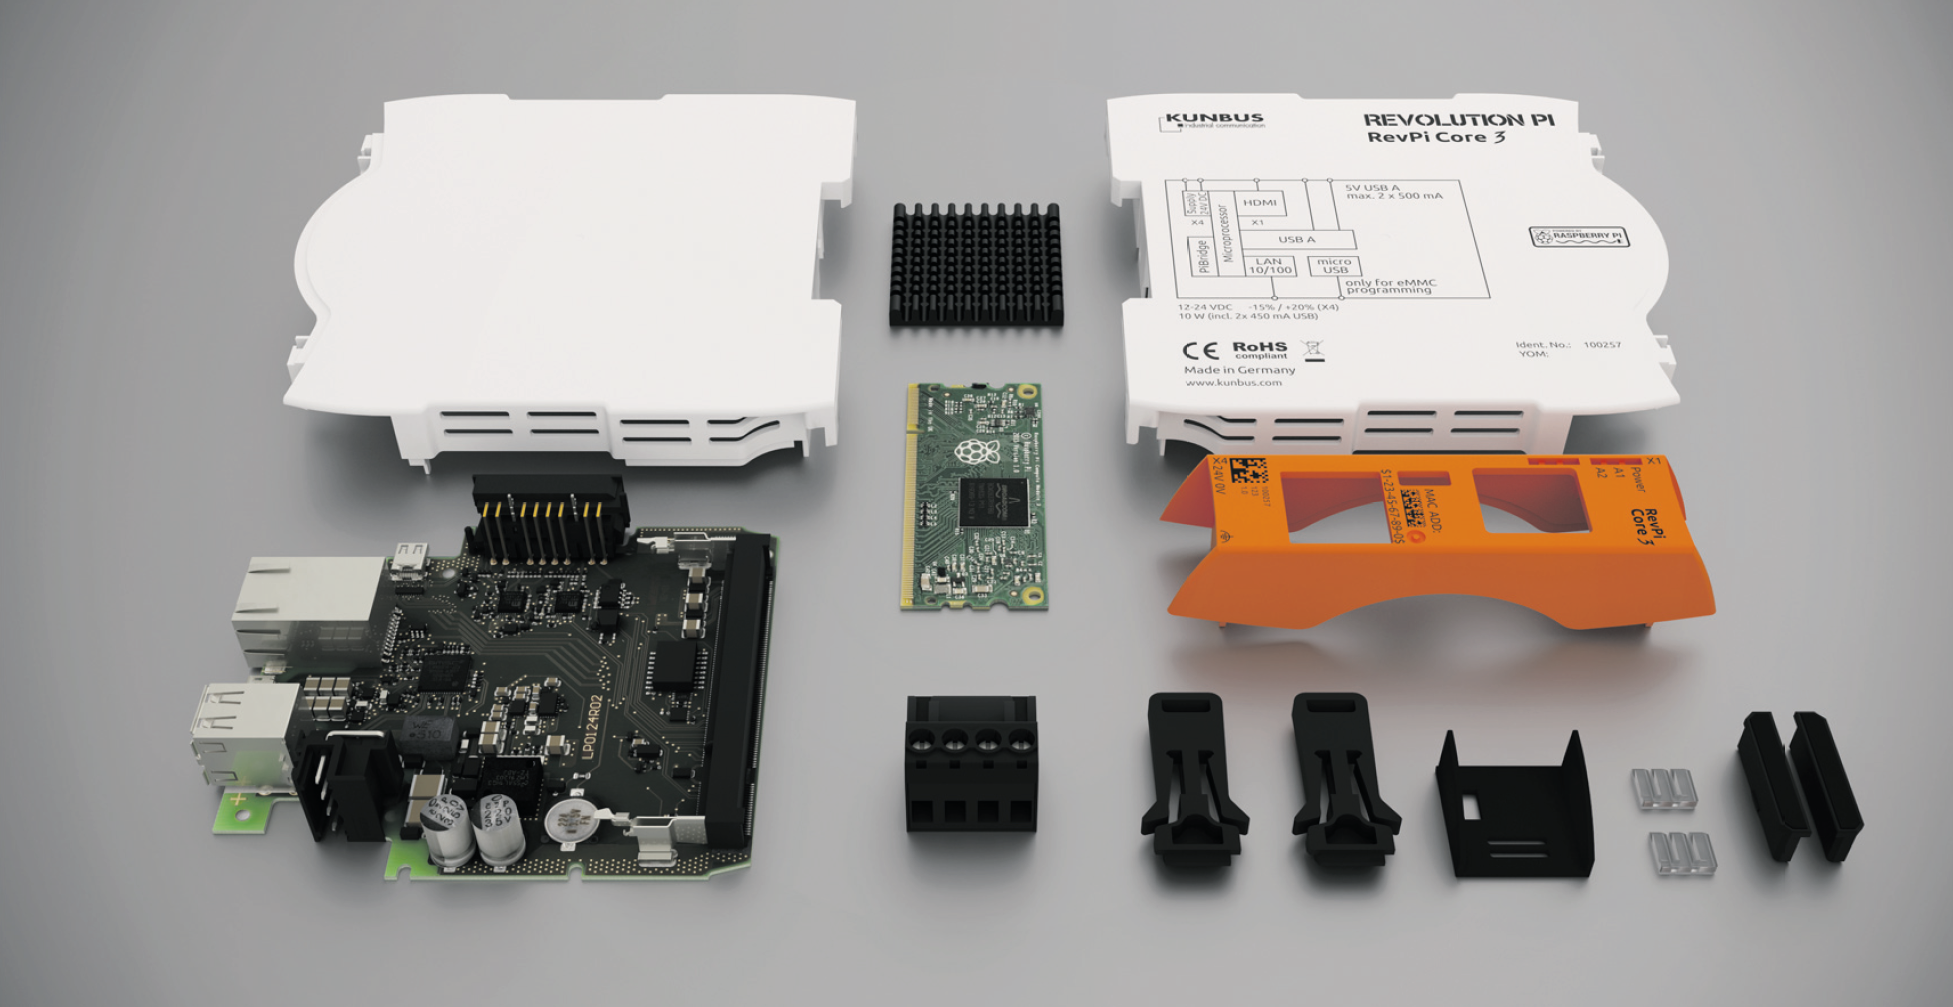
\includegraphics[width=0.85\textwidth]{doc/tex/images/revpi_teardown.png}
    \caption{Der RevPi Core 3 und seine Einzelkomponenten (Quelle: Kunbus)
      \label{fig:revpi-expl}}
\end{figure}

Spezifikationen des RevPi Core 3 \citep[Auswahl, vgl.][S. 1]{datasheet-revpi}:
\begin{itemize}
  \item{Prozessor: BCM2837}
  \item{Taktfrequenz 1,2 GHz}
  \item{Anzahl Prozessorkerne: 4}
  \item{Arbeitsspeicher: 1 GByte}
  \item{eMMC Flash Speicher: 4 GByte}
  \item{Betriebssystem: Angepasstes Raspbian mit RT-Patch}
  \item{RTC mit 24h Pufferung über wartungsfreien Kondensator}
  \item{Treiber / API: Kernel-Treiber schreibt zyklisch Prozessdaten in ein Prozessabbild, Zugriff auf Prozessabbild mittels ioctl-Anfragen oder über Linux-Dateisystem als API zu Fremdsoftware}
  \item{Kommunikationsanschlüsse: 2 x USB 2.0 A, 1 x Micro-USB, HDMI, Ethernet 10/100 Mbit/s}
  \item{Stromversorgung: min. 10,7 V, max. 28,8 V, maximal 10 Watt}
\end{itemize}

Kunbus stellt für den Revolution Pi ein auf Raspbian\footnote{Raspbian ist eine speziell 
für den Raspberry Pi angepasste Variante von Debian.} Stretch basierendes Betriebssystem bereit.
Verwendet wird der Kernel 4.9.76-rt60-v7+ in Verbindung mit dem SMP PREEMPT RT Patch.

\begin{figure}
    \centering
    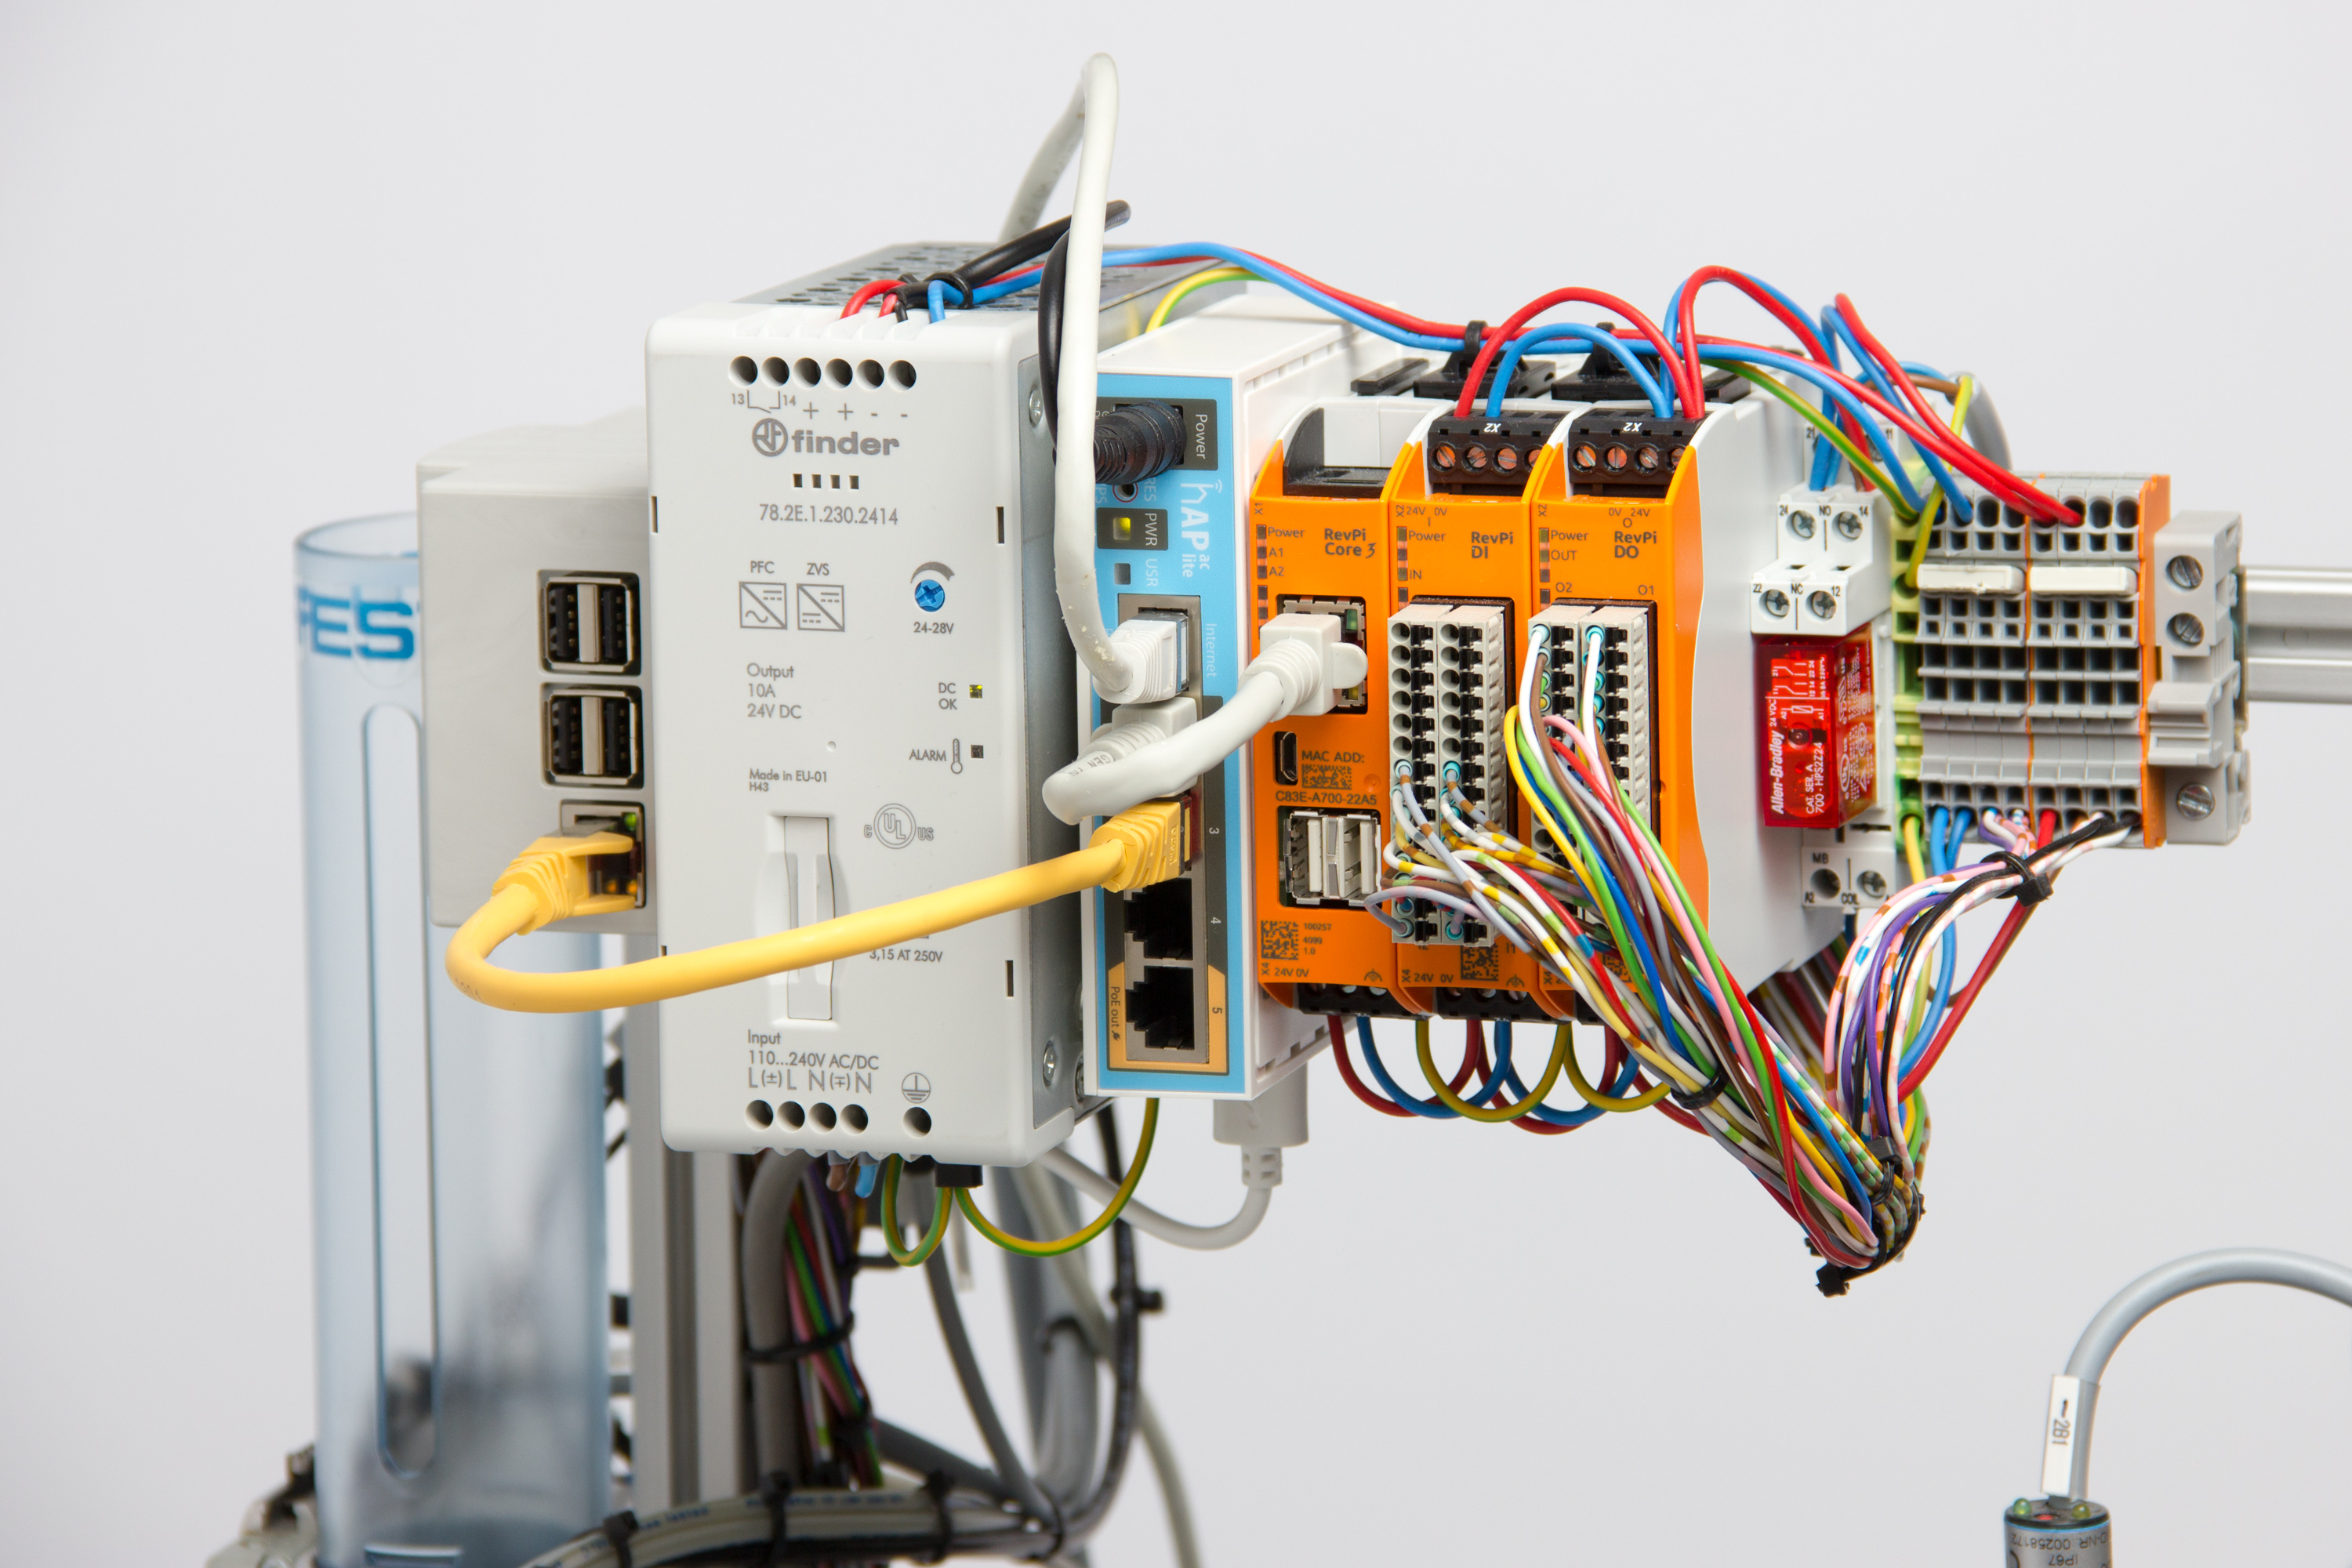
\includegraphics[trim={13cm 5cm 1cm 3cm}, clip, width=0.85\textwidth]{../photos/serverless_plc_img_8}
    \caption{Der Revolution Pi 3 mit digitalen IO-Modulen}
    \label{fig:rev-pi-io}
\end{figure}

Kunbus bietet neben dem sog. Core auch IO- und Gateway-Modulen zur Erweiterung der SPS an, siehe Bild~\ref{fig:rev-pi-io}.
Gateways dienen der Kommunikation mit externen Systemen oder Komponenten
über in der Automatisierungstechnik gängige Protokolle wie PROFIBUS oder EtherCAT. 
IO-Module erlauben die Überwachung und Steuerung von digitalen oder analogen Ein- und Ausgängen (IOs).

Kunbus deklariert die Hardware des Revolution Pi als Open-Source \citep[vgl.][S. 4]{flyer-revpi}. 
Die Schaltpläne des Revolution Pi, genauer die des RevPi Core 3 und der IO-Module, stehen auf der
Website\footnote{\label{downloads}\url{https://revolution.kunbus.com/tutorials/downloads/}} des Herstellers zum 
Download bereit. Eine Lizenz wird nicht angegeben.
Die Raspberry Pi Foundation stellt die Schaltpläne des Compute Modules des weiteren in ihrem Gitub-Repository 
zum Download bereit.

Sowohl die Raspberry Pi Foundation als auch die Kunbus GmbH pflegen aktiv ihre öffentlichen Repositories\footnote{\url{https://github.com/raspberrypi/} resp.~\url{https://github.com/RevolutionPi/}}
auf Github. 

% Kunbus konnte so einige Verbesserungen zum Linux Kernel 4.15 beitragen
% \footnote{siehe \url{https://revolution.kunbus.com/our-contribution-to-linux-4-15/}}.
% \todo{letzten Absatz evtl. weglassen? an sich nicht schlecht, passt aber irgendwie 
% nicht richtig zum Rest und stört den Lesefluss}

\subsubsection{Zugriff auf IO-Module%
        \label{sec:2-io}}
Der Zugriff auf die Ein- und Ausgänge der IO-Module erfolgt über einen RS485-Bus und einen in Form eines Kernel-Moduls bereitgestellten Treiber, genannt piControl. Der RS485-Bus ist über die serielle Schnittstelle des Compute Modules angebunden. 
piControl stellt ein Prozessabbild bereit, welches den physikalischen Zustand der Ein- und Ausgänge der IO-Module repräsentiert.
Das Prozessabbild wird, wie in der Automatisierungstechnik üblich, zyklisch aktualisiert. 
Die angestrebte Zykluszeit beträgt 5ms, kann jedoch je nach Anzahl der angeschlossenen Module auch größer sein. 
Kunbus garantiert bei drei IO-Modulen und zwei Gateway-Modulen eine Zykluszeit von 10 ms \citep[vgl.][]{web-revpi-dio}.
Die garantierte Zykluszeit ermöglicht die Umsetzung von Anwendungen mit harten Echtzeit-Anforderungen.

Fremdanwendungen können über eine Applikationsschnittstelle (API) auf das Prozessabbild zugreifen. 
Hierzu stellt das Kernel-Modul piControl sowohl \lstinline{seek}, \lstinline{read} und \lstinline{write} Methoden zur verfügung, wie auch die Möglichkeit mittels \lstinline{ioctl}-Anfragen gezielt auf einzelne Variablen des Prozessabbildes zuzugreifen.
In der englischsprachigen Wikipedia werden ioctl-Aufrufe wie folgt beschrieben:

\glqq{}The kernel is designed to be extensible, and may accept an extra module called a device driver which runs in kernel space and can directly address the device. An ioctl interface is a single system call by which userspace may communicate with device drivers. [...] The basic kernel can thus allow the userspace to access a device driver without knowing anything about the facilities supported by the device, and without needing an unmanageably large collection of system calls.

[...] ioctl calls provide a convenient way to bridge userspace code to kernel extensions. Kernel extensions can provide a location in the filesystem that can be opened by name, through which an arbitrary number of ioctl calls can be dispatched, allowing the extension to be programmed without adding system calls to the operating system.\grqq{}\citep[vgl.][]{web-wiki-ioctl}

Der Quellcode von piControl steht unter der GNU General Public License Version 2 (GNU GPLv2) und ist 
auf Github verfügbar\footnote{\url{https://github.com/RevolutionPi/piControl}}. Als Einstieg in die 
Entwicklung eigener Steuerungsprogramme liefert Kunbus das C-Programm piTest mit. Dieses verwendet 
piControl und erlaubt dem Nutzer über Kommandozeilen-Parameter die angeschlossenen IO-Module zu steuern.

\begin{figure}[h]
    \centering
    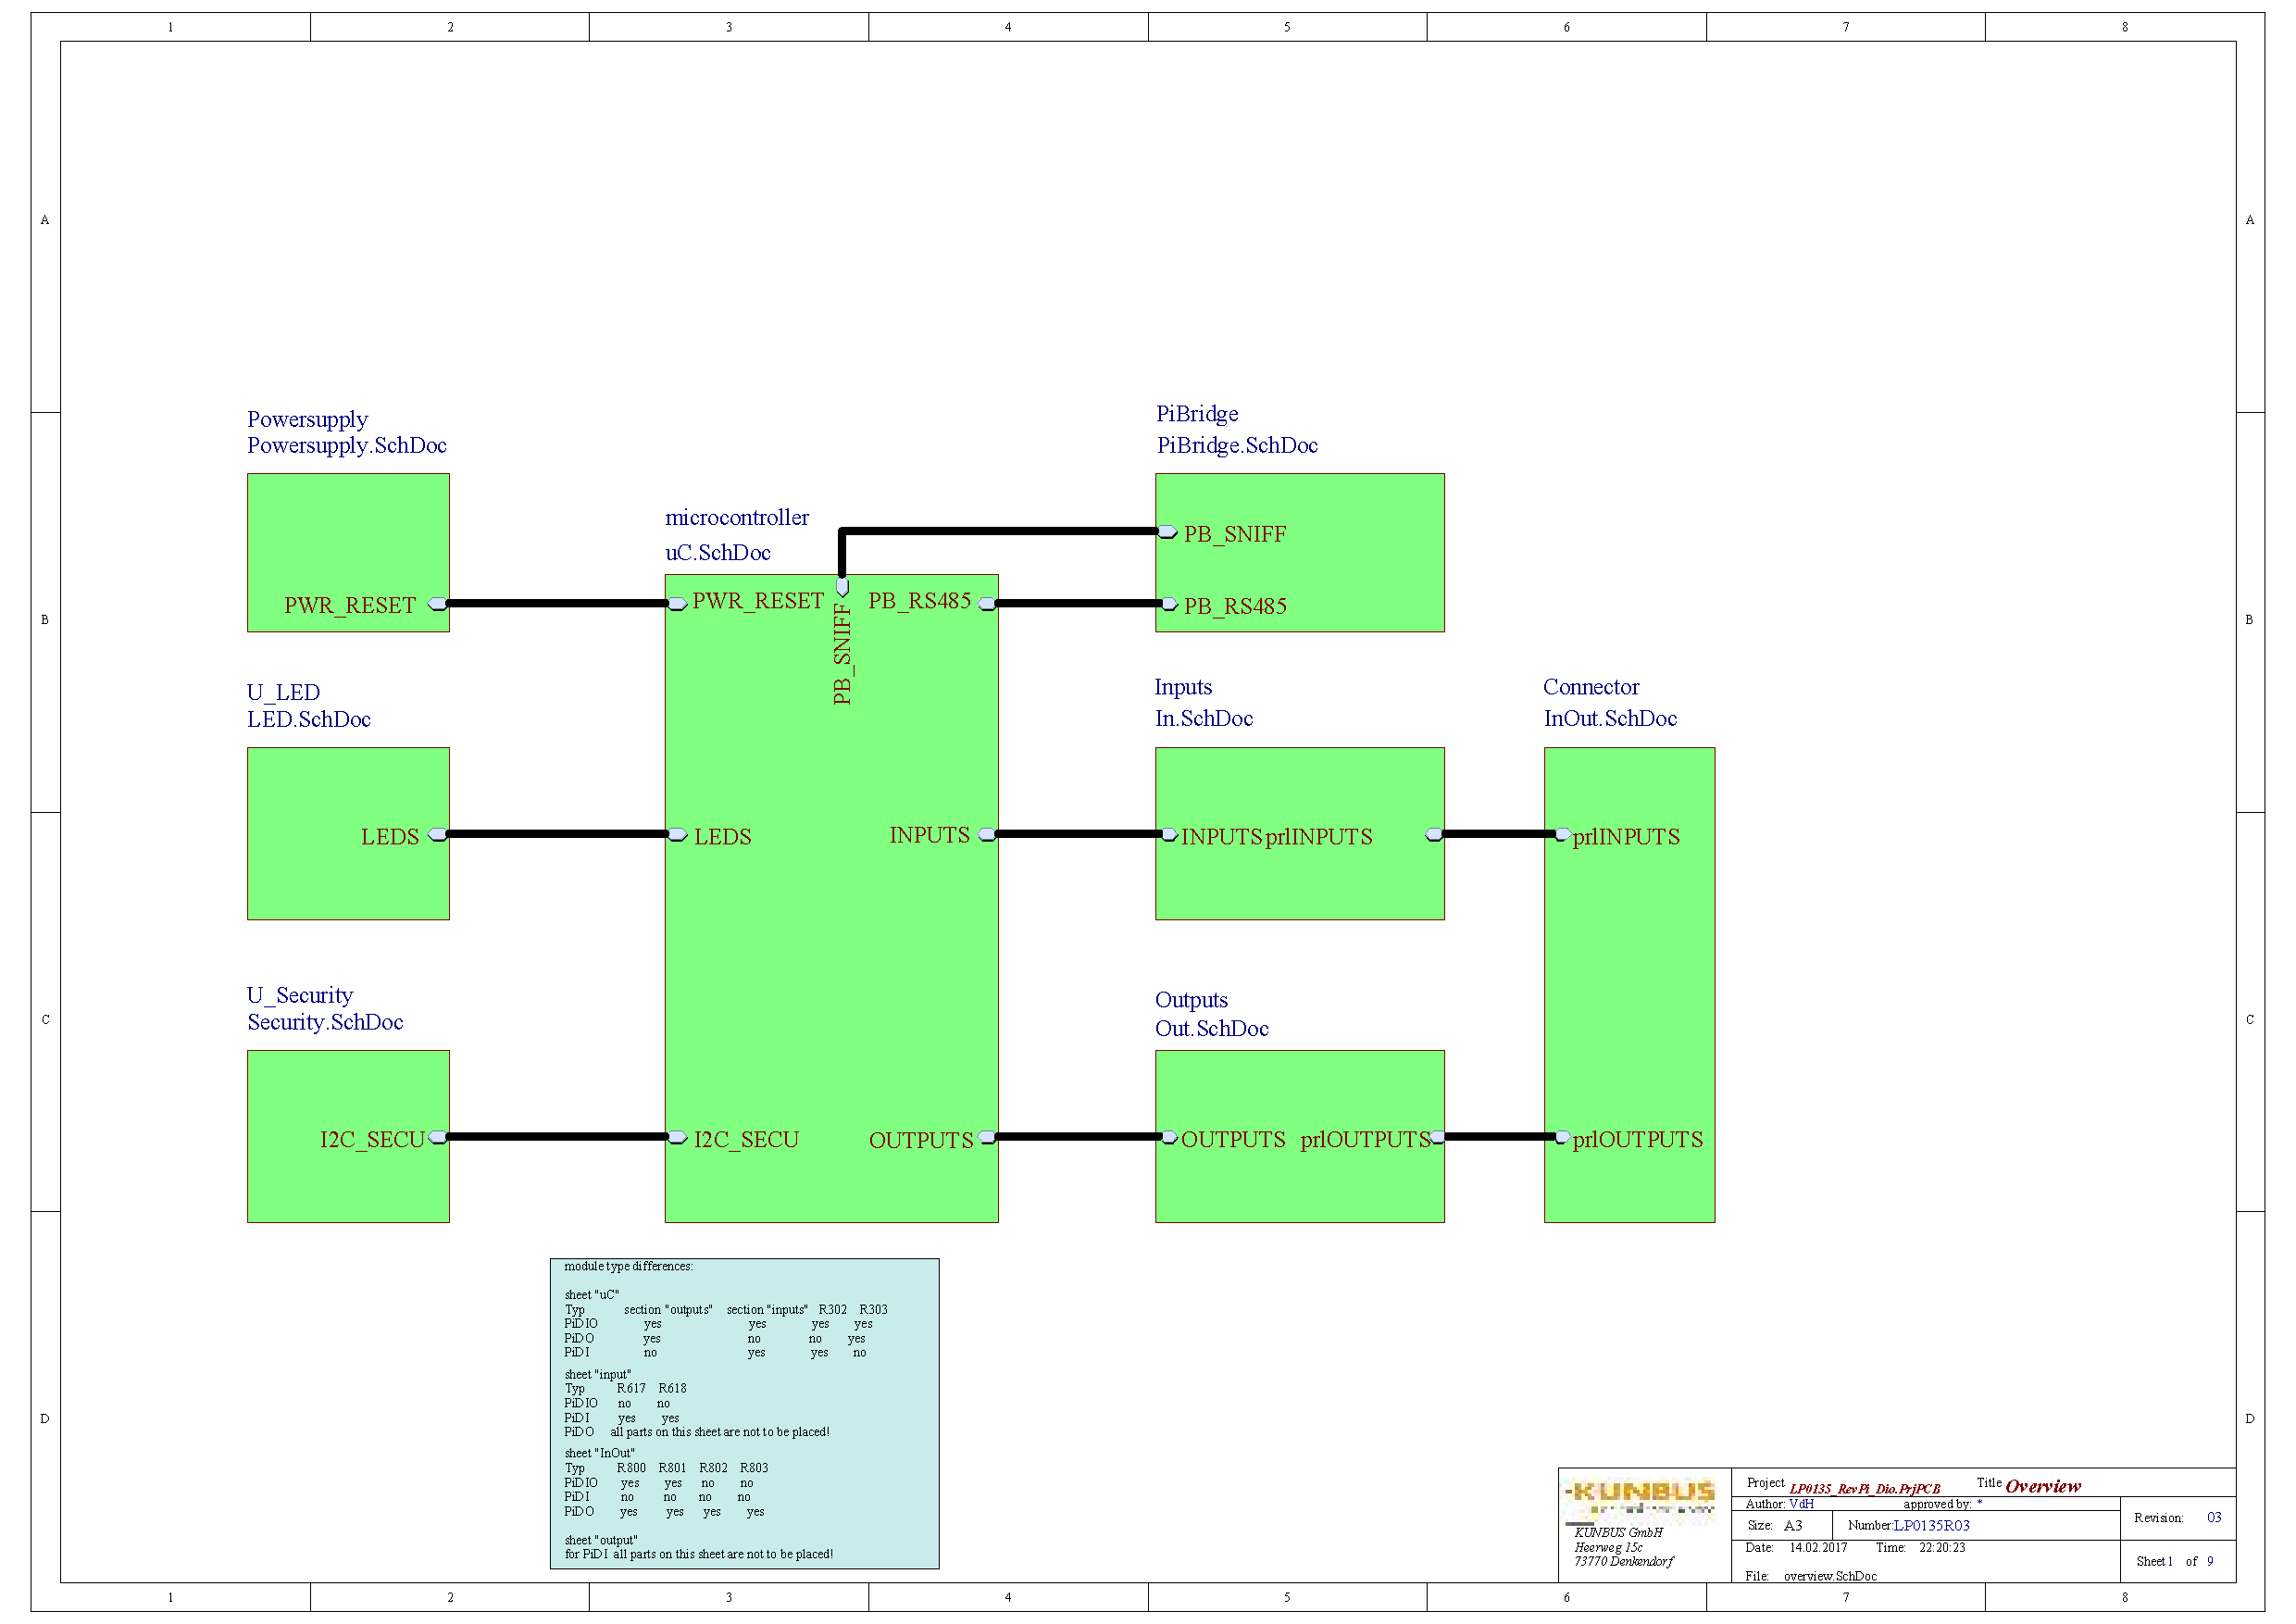
\includegraphics[trim={4cm 7cm 10.5cm 7.3cm}, clip, width=\textwidth]{literature/SchematicPrintsRevPi-DIO}
    \caption{Schematische Darstellung eines DIO-Moduls (Quelle: Kunbus\textsuperscript{\ref{downloads}})
      \label{fig:dio}}
\end{figure}

Jedes der IO-Module stellt ein eigenständiges eingebettetes System dar. Es verfügt
über einen Microcontroller, welcher die IOs bereitstellt und über einen RS485-Bus
mit dem Revolution Pi kommuniziert (siehe Bild~\ref{fig:dio}). 
Kunbus stellt exemplarisch den Quellcode eines DIO-Moduls unter der MIT Lizenz zur
Verfügung\footnote{\url{https://github.com/RevolutionPi/IODeviceExample}}. 


\subsection{Echtzeit und Multitasking unter Linux -- preemptRT und posix%
     \label{sec:2-echtzeit}}
     
Moderne Betriebssysteme realisieren Multitasking i.d.R.\,in Form des präemptiven Multitasking. 
Der Kernel verfügt über einen sog. Scheduler. Dieser priorisiert alle Prozesse und weist ihnen 
Rechenzeit in sog. Time Slots zu. Die Größe der Zeitfenster sowie die Ausführungsreihenfolge 
ist von der Priorität eines Prozesses abhängig. Besonders an einem präemptiven im Gegensatz zu einem kooperativen Scheduler ist dessen Fähigkeit, Tasks während ihrer Ausführung zu unterbrechen bzw. zu pausieren, wenn diese eine bestimmte Dauer überschreiten oder ein höher priorisierter Prozess (bspw. ausgelöst durch einen Interrupt oder durch eine inhärente Periodizität) Rechenleistung benötigt.

Eine Sonderform des präemptiven Multitasking ist das präemptible Multitasking. Hierbei werden auch Teile 
des Kernels als Threads durch den Scheduler ausgeführt. Dieser ist somit in der Lage, auch Prozesse des Kernels
zu unterbrechen, wenn andere Anwendungen Prozessorzeit oder Zugriff auf andere Systemressourcen benötigen
\citep[vgl.][]{web-wiki-praempt}.
     
Der Linux-Kernel implementiert unterschiedliche Präemptions-Modelle \citep[vgl.][/preemption\_models]{web-linuxwiki-basics}:

\begin{itemize}
  \item No Forced Preemption (server):
  Ausgelegt auf maximal möglichen Durchsatz, lediglich Interrupts und
  System-Call-Returns bewirken Präemption.

  \item Voluntary Kernel Preemption (Desktop):
  Neben den implizit bevorrechtigten Interrupts und System-Call-Returns gibt es
  in diesem Modell weitere Abschnitte des Kernels in welchen Preämption explizit
  gestattet ist.

  \item Preemptible Kernel (Low-Latency Desktop):
  In diesem Modell ist der gesamte Kernel, mit Ausnahme sog.~kritischer Abschnitte
  präemptible. Nach jedem kritischen Abschnitt gibt es einen impliziten Präemptions-Punkt.

  \item Preemptible Kernel (Basic RT):
  Dieses Modell ist dem zuvor genannten sehr ähnlich, hier sind jedoch alle Interrupt-Handler
  als eigenständige Threads ausgeführt.

  \item Fully Preemptible Kernel (RT):
  Wie auch bei den beiden zuvor genannten Modellen ist hier der gesamte Kernel
  präemtible. Die Anzahl und Dauer der nicht-präemtiblen kritischen Abschnitte
  ist auf ein notwendiges Minimum beschränkt. Alle Interrupt-Handler sind als
  eigenständige Threads ausgeführt, Spinlocks durch Sleeping-Spinlocks und Mutexe
  durch sog.~RT-Mutexe ersetzt.

\end{itemize}

Lediglich ein präemtibler Kernel kann hartes Echtzeit-Verhalten realisieren, 
da nur hier eine maximale Antwortzeit garantiert werden kann.
Viele Prozesse in der Automatisierungstechnik erfordern harte Echtzeit. 
Eine verspätete Antwort auf eine Anfrage, 
wie etwa das Signal eines Lagenendschalters oder eines Notausschalters kann hier nicht nur über
den Erfolg eines Prozesses, sondern auch über das Leben der daran beteiligten Mitarbeiter entscheiden.
Für weiterführende Erklärungen bzgl.\,Echtzeit, Mutexen und 
Spinlocks sei an dieser Stelle auf die Vorlesung verwiesen~\citep{script-peter}.


\subsubsection{preemptRT%
        \label{sec:2-preemptRT}}

Der Kernel des auf dem Revolution Pi installierten Raspbian mit PREEMP\_RT Patch fällt 
in die Kategorie des \glqq{}Fully Preemptible Kernels\grqq{} (siehe Abschnitt \ref{sec:2-echtzeit}).
Das zugrunde liegende Prinzip lässt sich wie folgt formulieren: Nur Code, welcher absolut nicht-präemtible sein darf, ist es
gestattet nicht-präemtible zu sein. Ziel ist folglich, die Menge des nicht-präemtiblen 
Codes im Linux-Kernel auf das absolut notwendige Minimum zu reduzieren.

Dies wird durch Verwendung folgender Mechanismen erreicht~\citep[vgl.][]{web-linuxwiki-details}:

\begin{itemize}
  \item Hochauflösende Timer
  \item Sleeping Spinlocks
  \item Threaded Interrupt Handlers
  \item rt\_mutex
  \item RCU
\end{itemize}

Diese Mechanismen sind bspw. im Linux-Wiki\footnote{siehe \url{https://wiki.linuxfoundation.org/realtime/documentation/technical_details}} ausführlich beschrieben.

\subsubsection{POSIX%
        \label{sec:2-posix}}
Das Portable Operating System Interface (POSIX) bezeichnet eine Sammlung von Standards, 
welche auf dem Unix-System basieren, jedoch nicht auf dieses beschränkt sind.

Der Wechsel zwischen verschiedenen Unix-Distributionen brachte oft Kompatibilitätsprobleme mit sich. 
Dieser Mangel an Portabilität erschwerte Benutzern und Entwicklern die Verwendung bzw. Bereitstellung 
von Software auf unterschiedlichen Systemen. 
Das Institut für Elektrotechnik und Elektronik (IEEE) begann 1984 mit der Entwicklung des Unix-Standards.
Sie entwickelten das, was heute als Single UNIX Specification bekannt ist und allgemein als POSIX bezeichnet wird~\citep[vgl.][]{web-debianwiki-posix}.
Das Konsortium \glqq{}The Open Group\grqq{} überwacht die weitere Entwicklung dieses Standards.
Ferner stellt es einen Teil der POSIX-Spezifikation frei zur Verfügung~\citep[vgl.][]{web-opengroup-posix}.

Die aktuelle Version POSIX.1-2017 ist verfügbar als IEEE Standard 1003.1-2017 sowie in Form der \glqq{}The Open Group Technical Standard Base Specifications\grqq{}, Ausgabe 7. POSIX.1-2017 definiert eine Standard-Betriebssystemschnittstelle und -umgebung, einschließlich eines Befehlsinterpreters (auch Shell genannt) und gängiger Dienstprogramme zur Unterstützung der Portabilität von Anwendungen auf Quellcode-Ebene. POSIX.1-2017 ist sowohl für Anwendungsentwickler als auch für Systemimplementierer gedacht und umfasst vier Hauptkomponenten \citep[vgl.][]{web-opengroup-overview}:
\begin{itemize}
    \item Basisdefinitionen:\\
          Allgemeine Begriffe, Konzepte und Schnittstellen einschließlich Hilfskonventionen und C-Headern
          
    \item Systemschnittstellen:\\
          Definitionen für Systemdienstfunktionen und Unterprogramme, C-spezifische Systemdienste, Portabilität
        
    \item Shell und Dienstprogramme:\\
          Definitionen für eine Schnittstelle zur Befehlsinterpretation von Diensten und gängige Hilfsprogramme
    
    \item Begründungen und Historie
\end{itemize}

Debian basiert auf Linux und verwendet den Linux-Kernel. Linux ist zu großen Teilen POSIX-kompatibel. Debian ist jedoch nicht POSIX-zertifiziert, da diese Zertifizierung mit hohen Kosten verbunden ist\citep[vgl.][Kapitel 4.4.]{web-debian-faq}.

Beide Kernkomponenten des in dieser Arbeit vorgestellten Projektes nutzen Komponenten von Linux, 
welche an den POSIX-Standard angelehnt sind: open62541 verwendet u.a.\,POSIX-Threads und
Mutexe~\citep[vgl.][pthread.h]{web-opengroup-pthread}, piControl nutzt POSIX-Semaphoren
\citep[vgl.][semaphore.h]{web-opengroup-semaphore}. 


\subsection{OPC-UA und open62541%
     \label{sec:2-opc}}
In diesem Abschnitt sollen Möglichkeiten des Datenaustausch zwischen Komponenten der
Automatisierungstechnik vorgestellt werden. OPC-UA stellt einen offenen, IP-basierten Kommunikationsstandard
für Sensoren und Steuerungen dar. open62541 ist eine freie Client- sowie Server-Implementierung dieses
Standards, geschrieben in C.


\subsubsection{OPC UA%
        \label{sec:2-opcua}}

Open Platform Communications (OPC) ist eine Familie von Standards zur herstellerunabhängigen
Kommunikation von Maschinen (M2M) in der Automatisierungstechnik. Die sog. OPC Task Force, zu deren
Mitgliedern verschiedene etablierte Firmen der Automatisierungsindustrie gehören, veröffentlichte
die OPC Specification Version 1.0 im August 1996.
Motiviert ist dieser offene Standard durch die Erkenntniss, dass die Anpassung der
zahlreichen Herstellerstandards an individuelle Infrastrukturen und Anlagen einen
großen Mehraufwand verursachen.
Die Wikipedia beschreibt das Anwendungsgebiet für OPC wie folgt \citep[vgl.][]{web-wiki-opc}:

\glqq{}OPC wird dort eingesetzt, wo Sensoren, Regler und Steuerungen verschiedener Hersteller
ein gemeinsames Netzwerk bilden. Ohne OPC benötigten zwei Geräte zum Datenaustausch
genaue Kenntnis über die Kommunikationsmöglichkeiten des Gegenübers. Erweiterungen
und Austausch gestalten sich entsprechend schwierig. Mit OPC genügt es, für jedes
Gerät genau einmal einen OPC-konformen Treiber zu schreiben. Idealerweise wird
dieser bereits vom Hersteller zur Verfügung gestellt. Ein OPC-Treiber lässt sich
ohne großen Anpassungsaufwand in beliebig große Steuer- und Überwachungssysteme
integrieren.

OPC unterteilt sich in verschiedene Unterstandards, die für den jeweiligen Anwendungsfall
unabhängig voneinander implementiert werden können. OPC lässt sich damit verwenden
für Echtzeitdaten (Überwachung), Datenarchivierung, Alarm-Meldungen und neuerdings
auch direkt zur Steuerung (Befehlsübermittlung).\grqq{}

OPC basiert in der ursprünglichen Spezifikation (auch als OPC DA bezeichnet) auf Microsofts DCOM-Spezifikation.
DCOM macht Funktionen und Objekte einer Anwendung anderen Anwendungen im Netzwerk
zugänglich. Der OPC-Standard definiert entsprechende DCOM-Objekte um mit anderen
OPC-Anwendungen Daten austauschen zu können. Die Verwendung von DCOM bindet Anwender
jedoch an Betriebssysteme von Microsoft. 

\begin{figure}
    \centering
    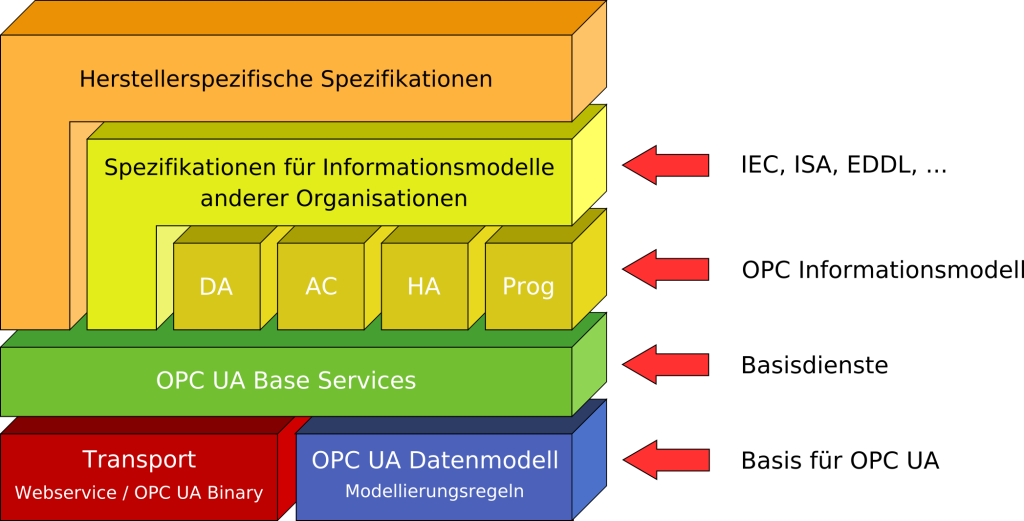
\includegraphics[width=0.85\textwidth]{images/UA_Architecture_1024.png}
    \caption{Die OPC Unified Architecture. Grafik von Gerhard Gappmeier - ascolab GmbH, CC BY-SA 3.0}
    \label{fig:opc-unified-architecture}
\end{figure}
% Evtl Grafik: Von Gerhard Gappmeier - ascolab GmbH, CC BY-SA 3.0, https://de.wikipedia.org/w/index.php?curid=1892069

Die ursprüngliche OPC Spezifikation wurde 2006 durch die Entwicklung der 
OPC Unified Architecture (OPC UA) überholt. 
Diese zeichnet sich durch eine Service-orientierte Architektur (SOA) aus, deren Struktur
aus mehreren Schichten besteht, siehe Abbilung~\ref{fig:opc-unified-architecture}. 
Über der untersten Schicht, dem Betriebssystem des Servers, verbindet eine Portabilitäts-Schicht 
den sog.\, UA ANSI C Stack mit einer API. Diese API kann bspw.\,in C++ geschrieben sein, 
und erlaubt die Anbindung der obersten Schicht, der Anwendungsschicht~\citep[vgl.][]{web-spec-opc}.
OPC UA setzt auf einem eigenen Kommunikationsstack auf; die Verwendung von DCOM
und damit die Bindung an Microsoft wurden aufgelöst.

Neben Architektur und Kommunikationsschnittstellen wird in der OPC Spezifikation auch ein 
Informationsmodell definiert. Die deutschsprachige Wikipedia beschreibt dieses wie folgt: 

\glqq{}Das OPC[-UA]-Informationsmodell ist nicht mehr nur eine Hierarchie aus Ordnern, Items
und Properties. Es ist ein sogenanntes Full-Mesh-Network aus Nodes, mit dem neben
den Nutzdaten eines Nodes auch Meta- und Diagnoseinformationen repräsentiert werden. [...]
Ein Node ähnelt einem Objekt aus der objektorientierten Programmierung. Ein Node
kann Attribute besitzen, die gelesen werden können. Es ist möglich Methoden zu definieren und aufzurufen. [...]
Weiterhin werden Events unterstützt, die versendet werden können
(AE (Alarms \& Events), DA DataChange), um bestimmte Informationen zwischen Geräten
auszutauschen. Ein Event besitzt unter anderem einen Empfangszeitpunkt, eine Nachricht
und einen Schweregrad. Die o.\,g. Nodes werden sowohl für die Nutzdaten als auch
alle anderen Arten von Metadaten verwendet. Der damit modellierte OPC-Adressraum
beinhaltet nun auch ein Typmodell, mit dem sämtliche Datentypen spezifiziert werden.\grqq{}


\subsubsection{open62541%
        \label{sec:2-open62541}}
open62541 ist eine offene und freie Implementierung von OPC UA. 
Die in C geschriebene Bibliothek stellt eine beständig zunehmende Anzahl der im OPC UA Standard definierten
Funktionen bereit. Sie kann sowohl zur Erstellung von OPC-Servern als auch von -Clients
genutzt werden. Ergänzend zu der unter der Mozilla Public License v2.0 lizensierten
Bibliothek stellt das open62541 Projekt auch Beispielprogramme unter einer CC0 Lizenz
zur Verfügung.
Zu den Unterstützern des Projektes zählen u.a.\, die RWTH Aachen, das Frauenhofer IOSB sowie die TU Dresden.

Die Bibliothek eignet sich auch für die Entwicklung auf eingebetteten Systemen und
Microcontrollern. Die Größe einer Server-Binary kann weniger als 100kB betragen.

Folgende Auswahl an Eigenschaften und Funktionen zeichnet die in dieser Arbeit verwendete
Version 0.3 von open62541 aus:
\begin{itemize}
  \item Kommunikationionsstack
  \begin{itemize}
      \item OPC UA Binär-Protokoll (HTTP oder SOAP werden gegenwärtig nicht unterstützt)
      \item Austauschbare Netzwerk-Schicht, welche die Verwendung eigener Netzwerk-APIs
      erlaubt.
      \item Verschlüsselte Kommunikationion
      \item Asynchrone Dienst-Anfragen im Client
  \end{itemize}
  \item Informationsmodell
  \begin{itemize}
    \item Unterstützung aller OPC UA Node-Typen, inkl.~Methoden
    \item Hinzufügen und Entfernen von Nodes und Referenzen zur Laufzeit.
    \item Vererbung und Instanziierung von Objekt- und Variablentypen
    \item Zugriffskontrolle auch für einzelne Nodes
  \end{itemize}
  \item Subscriptions
  \begin{itemize}
    \item Erlaubt die Überwachung (subscriptions / monitoreditems)
    \item Sehr geringer Ressourcenbedarf pro überwachtem Wert
  \end{itemize}
  \item Code-Generierung auf XML-Basis
  \begin{itemize}
    \item Erlaubt die Erstellung von Datentypen
    \item Erlaubt die Generierung des serverseitigen Informationsmodells
  \end{itemize}
\end{itemize}

Weiterführende Informationen und Code-Beispiele bietet die ausführliche Dokumentation des Projektes~\citep[siehe]{web-open62541} sowie der kommentierte Quelltext.

% % % Imports nur für Referenzenauflösung während des Schreibens! Vorm Kompilieren auskommentieren!
% \bibliography{0_hauptdatei}
% % Mit \section{...} eröffnen wir einen neuen Abschnitt.
% Der Befehl setzt nicht nur den Text in einer größeren,
% fetten Schrift, sondern sorgt außerdem dafür, daß er im
% Inhaltsverzeichnis erscheint.
%
% Mit \label{...} erzeugen wir einen Bezeichner, mit dessen Hilfe
% wir später auf die Nummer des Abschnitts verweisen können (nämlich
% mit~\ref{...}).
%
% Das Kommentarzeichen hinter „Übersicht“ dient dazu, ein
% Leerzeichen zwischen „Übersicht“ und dem \label-Befehl
% zu vermeiden, das andernfalls sichtbar würde – z.B. im
% Inhaltsverzeichnis.
%

% % Imports nur für Referenzenauflösung während des Schreibens! Vorm Kompilieren auskommentieren!
% \bibliography{0_hauptdatei}
% \input{1_einleitung}
%\input{2_grundlagen}
%\input{3_konzeption}
%\input{4_implementierung}
%\input{5_tests}
%\input{6_zusammenfassung}
% % Ende Imports

\section{Einleitung und Motivation%
  \label{sec:1-einleitung}}
Ziel dieses Projektes ist die Integration eines OPC-Servers mit einer auf Linux
basierenden speicherprogrammierbaren Steuerung (SPS). Angeschlossen an diese SPS
ist jeweils ein digitales Ein-/\,bzw.~Ausgabemodul. Die von diesen bereitgestellten
Ein-/\, bzw.~Ausgänge (IO) sollen in der Datenstruktur des OPC-Servers abgebildet
und über diesen für OPC-Clients les-/\,und schreibar sein. Weiterhin sollen einige
Funktionen zur Überwachung und Steuerung der an die SPS angeschlossenen Aktoren
und Sensoren direkt im OPC-Server implementiert werden.
Hiermit stellt dieses Projekt eine der Grundlagen für ein übergeordnetes Projekt,
die cloudbasierte Steuerung eines miniaturisierten Produktions-Systems, dar.

Der hier verwendete OPC-Server ist Teil des sog. open62541 Projekts. Er ist in C
geschrieben und implementiert bereits einen großen Teil der im OPC-UA-Standard
spezifizierten Funktionen.
Als SPS findet ein Revolution Pi 3 der Firma Kunbus Verwendung. Dieser integriert
ein sog. Compute Module der Raspberry Pi Foundation in ein industrietaugliches
Gehäuse und erlaubt die Erweiterung mittels IO- oder Gateway-Modulen. Über diese
erfolgt die Kommunikation mit weiteren Komponenten der Automatisierungstechnik.

Motiviert ist dieses Projekt durch die Beobachtung, dass die Verbreitung offener
Standards sowie freier Software auch in der Automatisierungstechnik zunimmt.
Linux ist ein freies Betriebssystem, OPC-UA ein offen zugänglicher, aktiv gepflegter
und weit verbreiteter Standard. Der Raspberry Pi findet sowohl bei Hobby-Anwendern als
auch in den Bereichen Forschung und Entwicklung sowie bei industriellen Anwendern
Verwendung. Dieses Projekt stellt somit eine für unterschiedliche Anwender interessante
Entwicklung dar.

Im Anschluss an diese einleitende Übersicht im Abschnitt~\ref{sec:1-einleitung} folgt
die Darstellung der wichtigsten Grundlagen in Abschnitt~\ref{sec:2-grundlagen}.
Aufbauend auf diesen Grundlagen folgt die konzeptuelle Ausarbeitung im Abschnitt~\ref{sec:3-konzeption}.
Die Umsetzung wird im Abschnitt~\ref{sec:4-implementierung} erläutert.
Die Leistungsfähigkeit der Implementierung wird in Abschnitt~\ref{sec:5-tests} untersucht.
Eine Zusammenfassung und ein Ausblick schließen die Arbeit in
Abschnitt~\ref{sec:6-fazit} ab. Eventuell noch benötigte Anhänge
finden sich in den Anhängen [...] bis [...].

% % % Imports nur für Referenzenauflösung während des Schreibens! Vorm Kompilieren auskommentieren!
% \bibliography{0_hauptdatei}
% \input{1_einleitung}
% \input{2_grundlagen}
% \input{3_konzeption}
% \input{4_implementierung}
% \input{5_tests}
% \input{6_zusammenfassung}
% % Ende Imports

\section{Grundlagen%
  \label{sec:2-grundlagen}}
Die folgenden Abschnitte bieten einen Überblick über die Verwendung offener Betriebssysteme und
Schnittstellen in der Automatisierungstechnik.
In Abschnitt~\ref{sec:2-sps} wird am Beispiel des Revolution Pi eine modulare Steuerung 
auf Basis von Linux vorgestellt. Ferner werden in Abschnitt~\ref{sec:2-echtzeit} die Themen Echtzeitfähigkeit und Portabilität von Software behandelt.

Eine große Zahl an Systemen in der Automatisierungstechnik ist heutzutage als eine Menge von Subsystemen mit
jeweils eigenem Speicher und Rechenleistung zu betrachten. Die zunehmende Komplexität von Fertigungsabläufen in Verbindung mit einer stetig abnehmenden Losgröße erfordert eine immer umfangreichere Kommunikation zwischen diesen Subsystemen.
Dies gelingt, insbesondere bei Verwendung von Komponenten unterschiedlicher Hersteller, nur mittels offener und flexibler Schnittstellen. OPC-UA stellt eine solche Schnittstelle dar und wird in Abschnitt~\ref{sec:2-opc} vorgestellt.

\subsection{Speicherprogrammierbare Steuerung auf Linux-Basis%
     \label{sec:2-sps}}
In diesem Abschnitt wird mit dem Revolution Pi eine Hard- und Softwarelösung zur Verwendung von Linux als Steuerung in der
Automatisierungstechnik vorgestellt.

\subsubsection{Kunbus Revolution Pi%
        \label{sec:2-revpi}}
Als Revolution Pi (RevPi) vertreibt die Firma Kunbus GmbH eine modulare, speicherprogrammierbare 
Steuerung (SPS). Zentrales Element dieser SPS ist der sog. RevPi Core, hier in der Version 3.
Kernkomponente des RevPi Core 3 ist das von der Raspberry Pi Foundation entwickelte und vertriebene 
Raspberry Pi Compute Module 3 (CM3, siehe Bild~\ref{fig:revpi-expl}. 
Die Architektur des CM3 ist weitgehend identisch zu der des allgemein bekannten Raspberry Pi 3.
Der RevPi Core 3 profitiert daher von dem selben großen Angebot an Software
und Unterstützung wie der Raspberry Pi. Er ergänzt dessen Hardware jedoch um eine 24V
Spannungsversorgung und die Möglichkeit der Erweiterung durch mehrere, zur industriellen 
Verwendung geeignete Ein- und Ausgabemodule (IO-Module. Die Integration dieser Merkmale in ein robustes Gehäuse 
mit Aufnahme für eine DIN-Schiene ermöglicht die Verwendung im industriellen Umfeld.

\begin{figure}[h]
    \centering
    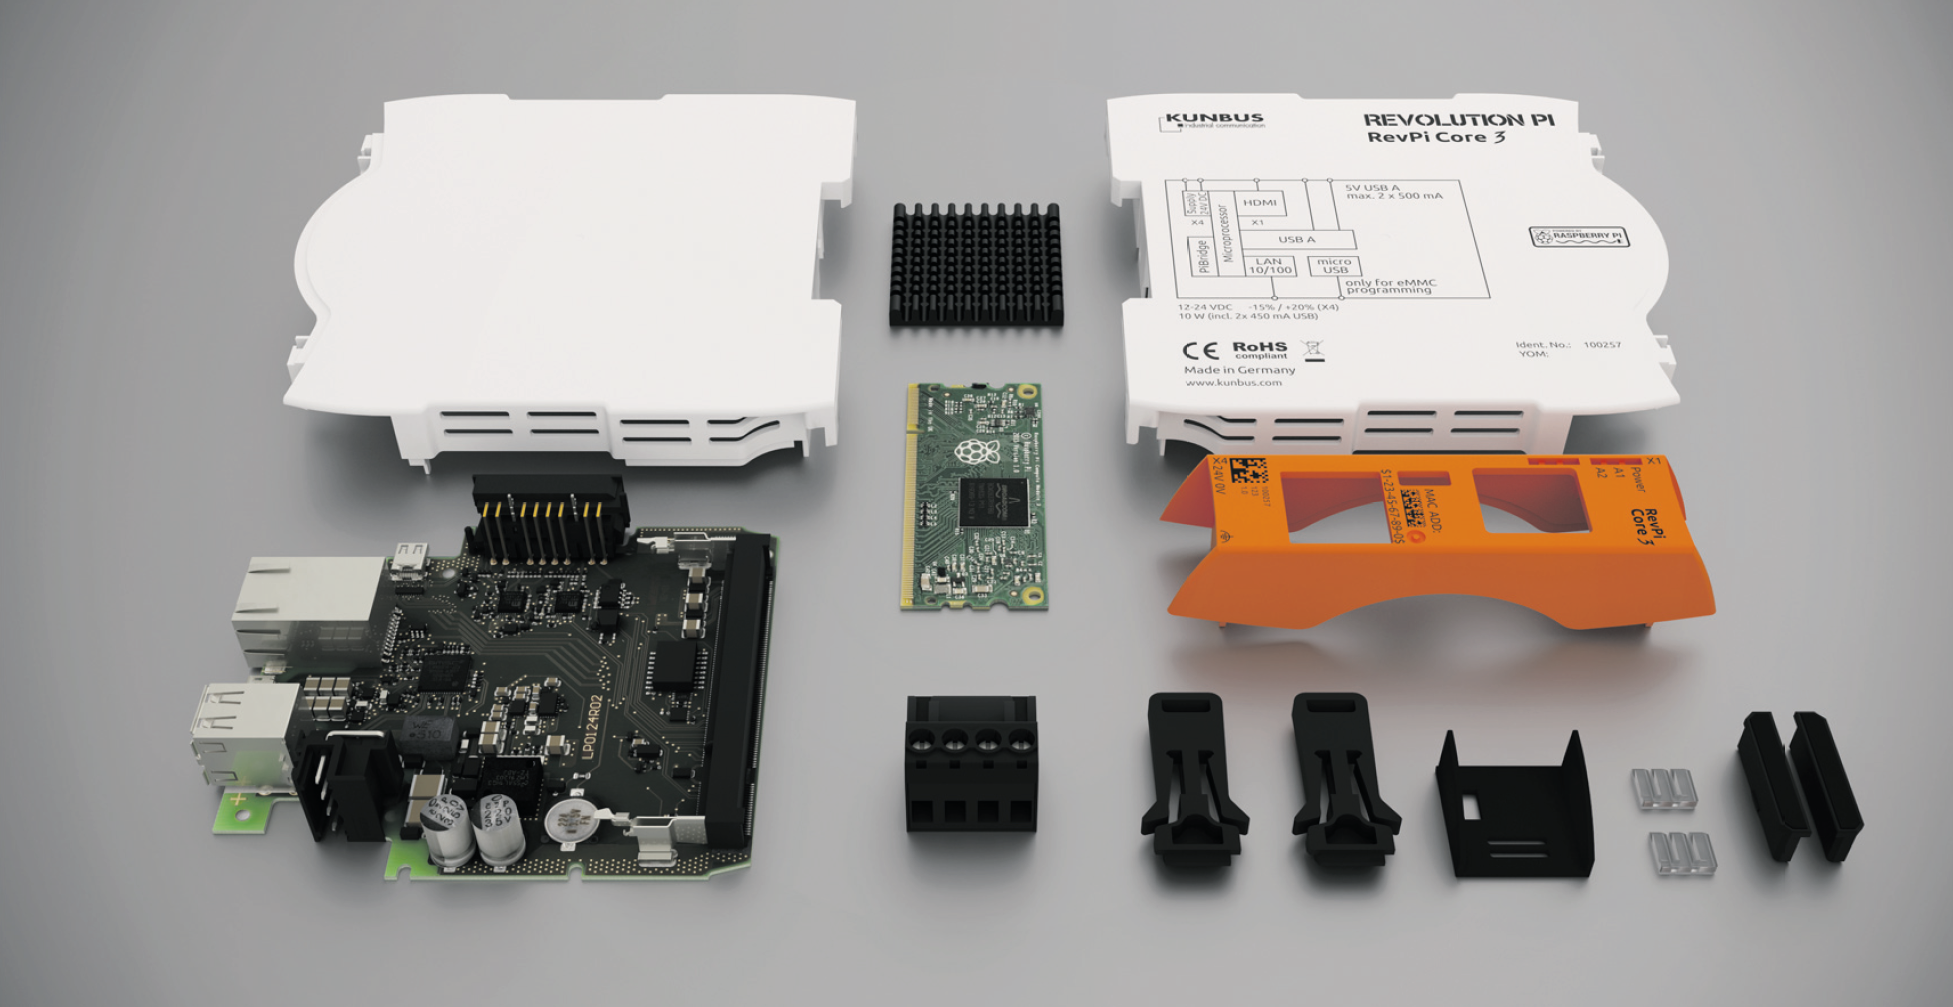
\includegraphics[width=0.85\textwidth]{doc/tex/images/revpi_teardown.png}
    \caption{Der RevPi Core 3 und seine Einzelkomponenten (Quelle: Kunbus)
      \label{fig:revpi-expl}}
\end{figure}

Spezifikationen des RevPi Core 3 \citep[Auswahl, vgl.][S. 1]{datasheet-revpi}:
\begin{itemize}
  \item{Prozessor: BCM2837}
  \item{Taktfrequenz 1,2 GHz}
  \item{Anzahl Prozessorkerne: 4}
  \item{Arbeitsspeicher: 1 GByte}
  \item{eMMC Flash Speicher: 4 GByte}
  \item{Betriebssystem: Angepasstes Raspbian mit RT-Patch}
  \item{RTC mit 24h Pufferung über wartungsfreien Kondensator}
  \item{Treiber / API: Kernel-Treiber schreibt zyklisch Prozessdaten in ein Prozessabbild, Zugriff auf Prozessabbild mittels ioctl-Anfragen oder über Linux-Dateisystem als API zu Fremdsoftware}
  \item{Kommunikationsanschlüsse: 2 x USB 2.0 A, 1 x Micro-USB, HDMI, Ethernet 10/100 Mbit/s}
  \item{Stromversorgung: min. 10,7 V, max. 28,8 V, maximal 10 Watt}
\end{itemize}

Kunbus stellt für den Revolution Pi ein auf Raspbian\footnote{Raspbian ist eine speziell 
für den Raspberry Pi angepasste Variante von Debian.} Stretch basierendes Betriebssystem bereit.
Verwendet wird der Kernel 4.9.76-rt60-v7+ in Verbindung mit dem SMP PREEMPT RT Patch.

\begin{figure}
    \centering
    \includegraphics[trim={13cm 5cm 1cm 3cm}, clip, width=0.85\textwidth]{../photos/serverless_plc_img_8}
    \caption{Der Revolution Pi 3 mit digitalen IO-Modulen}
    \label{fig:rev-pi-io}
\end{figure}

Kunbus bietet neben dem sog. Core auch IO- und Gateway-Modulen zur Erweiterung der SPS an, siehe Bild~\ref{fig:rev-pi-io}.
Gateways dienen der Kommunikation mit externen Systemen oder Komponenten
über in der Automatisierungstechnik gängige Protokolle wie PROFIBUS oder EtherCAT. 
IO-Module erlauben die Überwachung und Steuerung von digitalen oder analogen Ein- und Ausgängen (IOs).

Kunbus deklariert die Hardware des Revolution Pi als Open-Source \citep[vgl.][S. 4]{flyer-revpi}. 
Die Schaltpläne des Revolution Pi, genauer die des RevPi Core 3 und der IO-Module, stehen auf der
Website\footnote{\label{downloads}\url{https://revolution.kunbus.com/tutorials/downloads/}} des Herstellers zum 
Download bereit. Eine Lizenz wird nicht angegeben.
Die Raspberry Pi Foundation stellt die Schaltpläne des Compute Modules des weiteren in ihrem Gitub-Repository 
zum Download bereit.

Sowohl die Raspberry Pi Foundation als auch die Kunbus GmbH pflegen aktiv ihre öffentlichen Repositories\footnote{\url{https://github.com/raspberrypi/} resp.~\url{https://github.com/RevolutionPi/}}
auf Github. 

% Kunbus konnte so einige Verbesserungen zum Linux Kernel 4.15 beitragen
% \footnote{siehe \url{https://revolution.kunbus.com/our-contribution-to-linux-4-15/}}.
% \todo{letzten Absatz evtl. weglassen? an sich nicht schlecht, passt aber irgendwie 
% nicht richtig zum Rest und stört den Lesefluss}

\subsubsection{Zugriff auf IO-Module%
        \label{sec:2-io}}
Der Zugriff auf die Ein- und Ausgänge der IO-Module erfolgt über einen RS485-Bus und einen in Form eines Kernel-Moduls bereitgestellten Treiber, genannt piControl. Der RS485-Bus ist über die serielle Schnittstelle des Compute Modules angebunden. 
piControl stellt ein Prozessabbild bereit, welches den physikalischen Zustand der Ein- und Ausgänge der IO-Module repräsentiert.
Das Prozessabbild wird, wie in der Automatisierungstechnik üblich, zyklisch aktualisiert. 
Die angestrebte Zykluszeit beträgt 5ms, kann jedoch je nach Anzahl der angeschlossenen Module auch größer sein. 
Kunbus garantiert bei drei IO-Modulen und zwei Gateway-Modulen eine Zykluszeit von 10 ms \citep[vgl.][]{web-revpi-dio}.
Die garantierte Zykluszeit ermöglicht die Umsetzung von Anwendungen mit harten Echtzeit-Anforderungen.

Fremdanwendungen können über eine Applikationsschnittstelle (API) auf das Prozessabbild zugreifen. 
Hierzu stellt das Kernel-Modul piControl sowohl \lstinline{seek}, \lstinline{read} und \lstinline{write} Methoden zur verfügung, wie auch die Möglichkeit mittels \lstinline{ioctl}-Anfragen gezielt auf einzelne Variablen des Prozessabbildes zuzugreifen.
In der englischsprachigen Wikipedia werden ioctl-Aufrufe wie folgt beschrieben:

\glqq{}The kernel is designed to be extensible, and may accept an extra module called a device driver which runs in kernel space and can directly address the device. An ioctl interface is a single system call by which userspace may communicate with device drivers. [...] The basic kernel can thus allow the userspace to access a device driver without knowing anything about the facilities supported by the device, and without needing an unmanageably large collection of system calls.

[...] ioctl calls provide a convenient way to bridge userspace code to kernel extensions. Kernel extensions can provide a location in the filesystem that can be opened by name, through which an arbitrary number of ioctl calls can be dispatched, allowing the extension to be programmed without adding system calls to the operating system.\grqq{}\citep[vgl.][]{web-wiki-ioctl}

Der Quellcode von piControl steht unter der GNU General Public License Version 2 (GNU GPLv2) und ist 
auf Github verfügbar\footnote{\url{https://github.com/RevolutionPi/piControl}}. Als Einstieg in die 
Entwicklung eigener Steuerungsprogramme liefert Kunbus das C-Programm piTest mit. Dieses verwendet 
piControl und erlaubt dem Nutzer über Kommandozeilen-Parameter die angeschlossenen IO-Module zu steuern.

\begin{figure}[h]
    \centering
    \includegraphics[trim={4cm 7cm 10.5cm 7.3cm}, clip, width=\textwidth]{literature/SchematicPrintsRevPi-DIO}
    \caption{Schematische Darstellung eines DIO-Moduls (Quelle: Kunbus\textsuperscript{\ref{downloads}})
      \label{fig:dio}}
\end{figure}

Jedes der IO-Module stellt ein eigenständiges eingebettetes System dar. Es verfügt
über einen Microcontroller, welcher die IOs bereitstellt und über einen RS485-Bus
mit dem Revolution Pi kommuniziert (siehe Bild~\ref{fig:dio}). 
Kunbus stellt exemplarisch den Quellcode eines DIO-Moduls unter der MIT Lizenz zur
Verfügung\footnote{\url{https://github.com/RevolutionPi/IODeviceExample}}. 


\subsection{Echtzeit und Multitasking unter Linux -- preemptRT und posix%
     \label{sec:2-echtzeit}}
     
Moderne Betriebssysteme realisieren Multitasking i.d.R.\,in Form des präemptiven Multitasking. 
Der Kernel verfügt über einen sog. Scheduler. Dieser priorisiert alle Prozesse und weist ihnen 
Rechenzeit in sog. Time Slots zu. Die Größe der Zeitfenster sowie die Ausführungsreihenfolge 
ist von der Priorität eines Prozesses abhängig. Besonders an einem präemptiven im Gegensatz zu einem kooperativen Scheduler ist dessen Fähigkeit, Tasks während ihrer Ausführung zu unterbrechen bzw. zu pausieren, wenn diese eine bestimmte Dauer überschreiten oder ein höher priorisierter Prozess (bspw. ausgelöst durch einen Interrupt oder durch eine inhärente Periodizität) Rechenleistung benötigt.

Eine Sonderform des präemptiven Multitasking ist das präemptible Multitasking. Hierbei werden auch Teile 
des Kernels als Threads durch den Scheduler ausgeführt. Dieser ist somit in der Lage, auch Prozesse des Kernels
zu unterbrechen, wenn andere Anwendungen Prozessorzeit oder Zugriff auf andere Systemressourcen benötigen
\citep[vgl.][]{web-wiki-praempt}.
     
Der Linux-Kernel implementiert unterschiedliche Präemptions-Modelle \citep[vgl.][/preemption\_models]{web-linuxwiki-basics}:

\begin{itemize}
  \item No Forced Preemption (server):
  Ausgelegt auf maximal möglichen Durchsatz, lediglich Interrupts und
  System-Call-Returns bewirken Präemption.

  \item Voluntary Kernel Preemption (Desktop):
  Neben den implizit bevorrechtigten Interrupts und System-Call-Returns gibt es
  in diesem Modell weitere Abschnitte des Kernels in welchen Preämption explizit
  gestattet ist.

  \item Preemptible Kernel (Low-Latency Desktop):
  In diesem Modell ist der gesamte Kernel, mit Ausnahme sog.~kritischer Abschnitte
  präemptible. Nach jedem kritischen Abschnitt gibt es einen impliziten Präemptions-Punkt.

  \item Preemptible Kernel (Basic RT):
  Dieses Modell ist dem zuvor genannten sehr ähnlich, hier sind jedoch alle Interrupt-Handler
  als eigenständige Threads ausgeführt.

  \item Fully Preemptible Kernel (RT):
  Wie auch bei den beiden zuvor genannten Modellen ist hier der gesamte Kernel
  präemtible. Die Anzahl und Dauer der nicht-präemtiblen kritischen Abschnitte
  ist auf ein notwendiges Minimum beschränkt. Alle Interrupt-Handler sind als
  eigenständige Threads ausgeführt, Spinlocks durch Sleeping-Spinlocks und Mutexe
  durch sog.~RT-Mutexe ersetzt.

\end{itemize}

Lediglich ein präemtibler Kernel kann hartes Echtzeit-Verhalten realisieren, 
da nur hier eine maximale Antwortzeit garantiert werden kann.
Viele Prozesse in der Automatisierungstechnik erfordern harte Echtzeit. 
Eine verspätete Antwort auf eine Anfrage, 
wie etwa das Signal eines Lagenendschalters oder eines Notausschalters kann hier nicht nur über
den Erfolg eines Prozesses, sondern auch über das Leben der daran beteiligten Mitarbeiter entscheiden.
Für weiterführende Erklärungen bzgl.\,Echtzeit, Mutexen und 
Spinlocks sei an dieser Stelle auf die Vorlesung verwiesen~\citep{script-peter}.


\subsubsection{preemptRT%
        \label{sec:2-preemptRT}}

Der Kernel des auf dem Revolution Pi installierten Raspbian mit PREEMP\_RT Patch fällt 
in die Kategorie des \glqq{}Fully Preemptible Kernels\grqq{} (siehe Abschnitt \ref{sec:2-echtzeit}).
Das zugrunde liegende Prinzip lässt sich wie folgt formulieren: Nur Code, welcher absolut nicht-präemtible sein darf, ist es
gestattet nicht-präemtible zu sein. Ziel ist folglich, die Menge des nicht-präemtiblen 
Codes im Linux-Kernel auf das absolut notwendige Minimum zu reduzieren.

Dies wird durch Verwendung folgender Mechanismen erreicht~\citep[vgl.][]{web-linuxwiki-details}:

\begin{itemize}
  \item Hochauflösende Timer
  \item Sleeping Spinlocks
  \item Threaded Interrupt Handlers
  \item rt\_mutex
  \item RCU
\end{itemize}

Diese Mechanismen sind bspw. im Linux-Wiki\footnote{siehe \url{https://wiki.linuxfoundation.org/realtime/documentation/technical_details}} ausführlich beschrieben.

\subsubsection{POSIX%
        \label{sec:2-posix}}
Das Portable Operating System Interface (POSIX) bezeichnet eine Sammlung von Standards, 
welche auf dem Unix-System basieren, jedoch nicht auf dieses beschränkt sind.

Der Wechsel zwischen verschiedenen Unix-Distributionen brachte oft Kompatibilitätsprobleme mit sich. 
Dieser Mangel an Portabilität erschwerte Benutzern und Entwicklern die Verwendung bzw. Bereitstellung 
von Software auf unterschiedlichen Systemen. 
Das Institut für Elektrotechnik und Elektronik (IEEE) begann 1984 mit der Entwicklung des Unix-Standards.
Sie entwickelten das, was heute als Single UNIX Specification bekannt ist und allgemein als POSIX bezeichnet wird~\citep[vgl.][]{web-debianwiki-posix}.
Das Konsortium \glqq{}The Open Group\grqq{} überwacht die weitere Entwicklung dieses Standards.
Ferner stellt es einen Teil der POSIX-Spezifikation frei zur Verfügung~\citep[vgl.][]{web-opengroup-posix}.

Die aktuelle Version POSIX.1-2017 ist verfügbar als IEEE Standard 1003.1-2017 sowie in Form der \glqq{}The Open Group Technical Standard Base Specifications\grqq{}, Ausgabe 7. POSIX.1-2017 definiert eine Standard-Betriebssystemschnittstelle und -umgebung, einschließlich eines Befehlsinterpreters (auch Shell genannt) und gängiger Dienstprogramme zur Unterstützung der Portabilität von Anwendungen auf Quellcode-Ebene. POSIX.1-2017 ist sowohl für Anwendungsentwickler als auch für Systemimplementierer gedacht und umfasst vier Hauptkomponenten \citep[vgl.][]{web-opengroup-overview}:
\begin{itemize}
    \item Basisdefinitionen:\\
          Allgemeine Begriffe, Konzepte und Schnittstellen einschließlich Hilfskonventionen und C-Headern
          
    \item Systemschnittstellen:\\
          Definitionen für Systemdienstfunktionen und Unterprogramme, C-spezifische Systemdienste, Portabilität
        
    \item Shell und Dienstprogramme:\\
          Definitionen für eine Schnittstelle zur Befehlsinterpretation von Diensten und gängige Hilfsprogramme
    
    \item Begründungen und Historie
\end{itemize}

Debian basiert auf Linux und verwendet den Linux-Kernel. Linux ist zu großen Teilen POSIX-kompatibel. Debian ist jedoch nicht POSIX-zertifiziert, da diese Zertifizierung mit hohen Kosten verbunden ist\citep[vgl.][Kapitel 4.4.]{web-debian-faq}.

Beide Kernkomponenten des in dieser Arbeit vorgestellten Projektes nutzen Komponenten von Linux, 
welche an den POSIX-Standard angelehnt sind: open62541 verwendet u.a.\,POSIX-Threads und
Mutexe~\citep[vgl.][pthread.h]{web-opengroup-pthread}, piControl nutzt POSIX-Semaphoren
\citep[vgl.][semaphore.h]{web-opengroup-semaphore}. 


\subsection{OPC-UA und open62541%
     \label{sec:2-opc}}
In diesem Abschnitt sollen Möglichkeiten des Datenaustausch zwischen Komponenten der
Automatisierungstechnik vorgestellt werden. OPC-UA stellt einen offenen, IP-basierten Kommunikationsstandard
für Sensoren und Steuerungen dar. open62541 ist eine freie Client- sowie Server-Implementierung dieses
Standards, geschrieben in C.


\subsubsection{OPC UA%
        \label{sec:2-opcua}}

Open Platform Communications (OPC) ist eine Familie von Standards zur herstellerunabhängigen
Kommunikation von Maschinen (M2M) in der Automatisierungstechnik. Die sog. OPC Task Force, zu deren
Mitgliedern verschiedene etablierte Firmen der Automatisierungsindustrie gehören, veröffentlichte
die OPC Specification Version 1.0 im August 1996.
Motiviert ist dieser offene Standard durch die Erkenntniss, dass die Anpassung der
zahlreichen Herstellerstandards an individuelle Infrastrukturen und Anlagen einen
großen Mehraufwand verursachen.
Die Wikipedia beschreibt das Anwendungsgebiet für OPC wie folgt \citep[vgl.][]{web-wiki-opc}:

\glqq{}OPC wird dort eingesetzt, wo Sensoren, Regler und Steuerungen verschiedener Hersteller
ein gemeinsames Netzwerk bilden. Ohne OPC benötigten zwei Geräte zum Datenaustausch
genaue Kenntnis über die Kommunikationsmöglichkeiten des Gegenübers. Erweiterungen
und Austausch gestalten sich entsprechend schwierig. Mit OPC genügt es, für jedes
Gerät genau einmal einen OPC-konformen Treiber zu schreiben. Idealerweise wird
dieser bereits vom Hersteller zur Verfügung gestellt. Ein OPC-Treiber lässt sich
ohne großen Anpassungsaufwand in beliebig große Steuer- und Überwachungssysteme
integrieren.

OPC unterteilt sich in verschiedene Unterstandards, die für den jeweiligen Anwendungsfall
unabhängig voneinander implementiert werden können. OPC lässt sich damit verwenden
für Echtzeitdaten (Überwachung), Datenarchivierung, Alarm-Meldungen und neuerdings
auch direkt zur Steuerung (Befehlsübermittlung).\grqq{}

OPC basiert in der ursprünglichen Spezifikation (auch als OPC DA bezeichnet) auf Microsofts DCOM-Spezifikation.
DCOM macht Funktionen und Objekte einer Anwendung anderen Anwendungen im Netzwerk
zugänglich. Der OPC-Standard definiert entsprechende DCOM-Objekte um mit anderen
OPC-Anwendungen Daten austauschen zu können. Die Verwendung von DCOM bindet Anwender
jedoch an Betriebssysteme von Microsoft. 

\begin{figure}
    \centering
    \includegraphics[width=0.85\textwidth]{images/UA_Architecture_1024.png}
    \caption{Die OPC Unified Architecture. Grafik von Gerhard Gappmeier - ascolab GmbH, CC BY-SA 3.0}
    \label{fig:opc-unified-architecture}
\end{figure}
% Evtl Grafik: Von Gerhard Gappmeier - ascolab GmbH, CC BY-SA 3.0, https://de.wikipedia.org/w/index.php?curid=1892069

Die ursprüngliche OPC Spezifikation wurde 2006 durch die Entwicklung der 
OPC Unified Architecture (OPC UA) überholt. 
Diese zeichnet sich durch eine Service-orientierte Architektur (SOA) aus, deren Struktur
aus mehreren Schichten besteht, siehe Abbilung~\ref{fig:opc-unified-architecture}. 
Über der untersten Schicht, dem Betriebssystem des Servers, verbindet eine Portabilitäts-Schicht 
den sog.\, UA ANSI C Stack mit einer API. Diese API kann bspw.\,in C++ geschrieben sein, 
und erlaubt die Anbindung der obersten Schicht, der Anwendungsschicht~\citep[vgl.][]{web-spec-opc}.
OPC UA setzt auf einem eigenen Kommunikationsstack auf; die Verwendung von DCOM
und damit die Bindung an Microsoft wurden aufgelöst.

Neben Architektur und Kommunikationsschnittstellen wird in der OPC Spezifikation auch ein 
Informationsmodell definiert. Die deutschsprachige Wikipedia beschreibt dieses wie folgt: 

\glqq{}Das OPC[-UA]-Informationsmodell ist nicht mehr nur eine Hierarchie aus Ordnern, Items
und Properties. Es ist ein sogenanntes Full-Mesh-Network aus Nodes, mit dem neben
den Nutzdaten eines Nodes auch Meta- und Diagnoseinformationen repräsentiert werden. [...]
Ein Node ähnelt einem Objekt aus der objektorientierten Programmierung. Ein Node
kann Attribute besitzen, die gelesen werden können. Es ist möglich Methoden zu definieren und aufzurufen. [...]
Weiterhin werden Events unterstützt, die versendet werden können
(AE (Alarms \& Events), DA DataChange), um bestimmte Informationen zwischen Geräten
auszutauschen. Ein Event besitzt unter anderem einen Empfangszeitpunkt, eine Nachricht
und einen Schweregrad. Die o.\,g. Nodes werden sowohl für die Nutzdaten als auch
alle anderen Arten von Metadaten verwendet. Der damit modellierte OPC-Adressraum
beinhaltet nun auch ein Typmodell, mit dem sämtliche Datentypen spezifiziert werden.\grqq{}


\subsubsection{open62541%
        \label{sec:2-open62541}}
open62541 ist eine offene und freie Implementierung von OPC UA. 
Die in C geschriebene Bibliothek stellt eine beständig zunehmende Anzahl der im OPC UA Standard definierten
Funktionen bereit. Sie kann sowohl zur Erstellung von OPC-Servern als auch von -Clients
genutzt werden. Ergänzend zu der unter der Mozilla Public License v2.0 lizensierten
Bibliothek stellt das open62541 Projekt auch Beispielprogramme unter einer CC0 Lizenz
zur Verfügung.
Zu den Unterstützern des Projektes zählen u.a.\, die RWTH Aachen, das Frauenhofer IOSB sowie die TU Dresden.

Die Bibliothek eignet sich auch für die Entwicklung auf eingebetteten Systemen und
Microcontrollern. Die Größe einer Server-Binary kann weniger als 100kB betragen.

Folgende Auswahl an Eigenschaften und Funktionen zeichnet die in dieser Arbeit verwendete
Version 0.3 von open62541 aus:
\begin{itemize}
  \item Kommunikationionsstack
  \begin{itemize}
      \item OPC UA Binär-Protokoll (HTTP oder SOAP werden gegenwärtig nicht unterstützt)
      \item Austauschbare Netzwerk-Schicht, welche die Verwendung eigener Netzwerk-APIs
      erlaubt.
      \item Verschlüsselte Kommunikationion
      \item Asynchrone Dienst-Anfragen im Client
  \end{itemize}
  \item Informationsmodell
  \begin{itemize}
    \item Unterstützung aller OPC UA Node-Typen, inkl.~Methoden
    \item Hinzufügen und Entfernen von Nodes und Referenzen zur Laufzeit.
    \item Vererbung und Instanziierung von Objekt- und Variablentypen
    \item Zugriffskontrolle auch für einzelne Nodes
  \end{itemize}
  \item Subscriptions
  \begin{itemize}
    \item Erlaubt die Überwachung (subscriptions / monitoreditems)
    \item Sehr geringer Ressourcenbedarf pro überwachtem Wert
  \end{itemize}
  \item Code-Generierung auf XML-Basis
  \begin{itemize}
    \item Erlaubt die Erstellung von Datentypen
    \item Erlaubt die Generierung des serverseitigen Informationsmodells
  \end{itemize}
\end{itemize}

Weiterführende Informationen und Code-Beispiele bietet die ausführliche Dokumentation des Projektes~\citep[siehe]{web-open62541} sowie der kommentierte Quelltext.

% % % Imports nur für Referenzenauflösung während des Schreibens! Vorm Kompilieren auskommentieren!
% \bibliography{0_hauptdatei}
% \input{1_einleitung}
% \input{2_grundlagen}
% \input{3_konzeption}
% \input{4_implementierung}
% \input{5_tests}
% \input{6_zusammenfassung}
% \input{anhang}
% % Ende Imports

\section{Systemkonzept%
  \label{sec:3-konzeption}}
Auf Basis der in Abschnitt [...] vorgestellten Möglichkeiten folgt nun die Ausarbeitung eines Konzepts.

\subsection{Anbindung der IO an den OPC-Server%
     \label{sec:3-anbindung}}

\subsection{Integration des OPC-Servers in das System%
     \label{sec:3-integration}}

% % % Imports nur für Referenzenauflösung während des Schreibens! Vorm Kompilieren auskommentieren!
% \bibliography{0_hauptdatei}
% \input{1_einleitung}
% \input{2_grundlagen}
% \input{3_konzeption}
% \input{4_implementierung}
% \input{5_tests}
% \input{6_zusammenfassung}
% \input{anhang}
% % Ende Imports

\section{Implementierung%
  \label{sec:4-implementierung}}
Das folgende Kapitel stellt in Auszügen die Implementierung des OPC-Servers sowie die Anbindung an die IO-Module
der SPS dar. Der Schwerpunkt liegt hierbei auf der Funktionsweise des piControl-Treibers und dessen Integration in das Projekt. Abschnitt~\ref{sec:4-picontrol} erklärt die zum Schreibens eines Bits verwendeten Funktionsaufrufe.
Zuvor soll jedoch in Abschnitt~\ref{sec:4-open62541} der Teil des OPC-Servers vorgestellt werden, welcher auf besagten Treiber zugreift. 

\subsection{Implementierung des OPC-Servers%
     \label{sec:4-open62541}}
Wie im vorangegangenen Abschnitt~\ref{sec:3-integration} begründet, soll die Verknüpfung zwischen dem Prozessabbild der SPS und den auf dem OPC-Server bereitgestellten Werten über sog.\,Datenquellen erfolgen. Hierzu ist zunächst eine Callback-Methode zu implementieren, welche bei einem Lese- oder Schreibzugriff auf eine Variable aufgerufen wird. Die Verknüpfung zwischen Callback-Methode und Variable muss manuell erfolgen.

\begin{lstlisting}[language={c},firstnumber=237,caption={Auszug der Methode \lstinline{linkDataSourceVariable} in \lstinline{variables.c}\label{lst:4-linkDataSourceVariable}}]
extern UA_StatusCode
 linkDataSourceVariable(UA_Server *server, UA_NodeId nodeId) {
     bool readonly = false;
     UA_DataSource dataSourceVariable;
     UA_StatusCode rc; |>\setcounter{lstnumber}{254}<|

     dataSourceVariable.read = readDataSourceVariable;
     if (!readonly)
        dataSourceVariable.write = writeDataSourceVariable;
     else
        dataSourceVariable.write = writeReadonlyDataSourceVariable;

     return UA_Server_setVariableNode_dataSource(server, nodeId, dataSourceVariable);
 }
\end{lstlisting}

\begin{figure}[h]
    \centering
    \includegraphics[width=0.42\textwidth]{doc/img/OPC_RevPiDO.pdf}
    \caption{Auszug des verwendeten Nodesets, hier Digitalausgang 1 des Versuchsaufbaus
      \label{fig:opc-do}}
\end{figure}

Die in Listing~\ref{lst:4-linkDataSourceVariable} abgebildete Methode \lstinline{linkDataSourceVariable()} erzeugt ein Struct vom Typ \lstinline{UA_DataSource}. In diesem werden dem Lesen und Schreiben einer OPC-Variablen entsprechende Callback-Methoden zugewiesen. Die Verknüpfung einer OPC-Variable, genauer ihrer NodeId, mit der zuvor definierten Datenquelle erfolgt über die von open62541 bereitgestellte Methode \lstinline{UA_Server_setVariableNode_dataSource()}. Vor dem Lesen und nach dem Schreiben dieser Variable werden von nun an die entsprechenden Callbacks aufgerufen.
     
\begin{lstlisting}[language={c},firstnumber=168,caption={Auszug des Callbacks \lstinline{writeDataSourceVariable} in \lstinline{variables.c}\label{lst:4-writeDataSourceVariable}}]  
extern UA_StatusCode
 writeDataSourceVariable(UA_Server *server,
            const UA_NodeId *sessionId, void *sessionContext,
            const UA_NodeId *nodeId, void *nodeContext,
            const UA_NumericRange *range, const UA_DataValue *dataValue) {

    UA_StatusCode retval  = UA_STATUSCODE_GOOD;
    UA_NodeId *nameNodeId = UA_malloc(sizeof(UA_NodeId));
    UA_QualifiedName nameQN = UA_QUALIFIEDNAME(1, "Name");
    UA_Variant nameVar;
    UA_Boolean bit;

    retval |= findSiblingByBrowsename(server, nodeId, &nameQN, nameNodeId);
    retval |= UA_Server_readValue(server, *nameNodeId, &nameVar);
    retval |= UA_Boolean_copy(dataValue->value.data, &bit);

    |>\tikzmarkin[set border color=martinired]{writeIO}<|PI_writeSingleIO(String_fromUA_String(nameVar.data), &bit, false);                                                 |>\tikzmarkend{writeIO}<|

    free(nameNodeId);
    return retval;
 }
\end{lstlisting}

Listing~\ref{lst:4-writeDataSourceVariable} zeigt die Callback-Methode, welche nach dem Schreiben einer Variablen auf dem OPC-Server aufgerufen wird.
Dieser Methode wird neben der NodeId der mit ihr verknüpften Variablen auch der Wert dieser in Form eines Zeigers auf ein Struct vom Typ \lstinline{UA_DataValue} übergeben.

Die Gestaltung des hier verwendeten Nodesets sieht vor, dass in einer OPC-Variablen \lstinline{"Name"} der Bezeichner des zu schreibenden Digitalausgangs hinterlegt ist, siehe Abbildung~\ref{fig:opc-do}. Dies erlaubt eine Rekonfiguration der Ein- und Ausgänge der SPS ohne Änderungen im Programmcode des OPC-Servers vornehmen zu müssen.
Es ist daher erforderlich, nach jedem Schreiben einer mit einem Digitalausgang verknüpften Variablen, hier \lstinline{"Value"}, dessen Bezeichner \lstinline{"Name"} abzufragen. 
Dies geschieht in den Zeilen 180 und 181.
Anschließend wird dieser Bezeichner sowie der zu schreibende Wert der Methode \lstinline{PI_writeSingleIO()} übergeben, welche wiederum die Interaktion mit piControl übernimmt (vgl. Abschnitt \ref{sec:4-picontrol}).
 
\subsection{Integration von piControl%
     \label{sec:4-picontrol}}
In Abschnitt~\ref{sec:2-io} wurde die Anbindung der IO-Module des Revolution Pi sowie die Funktionsweise von piControl aus Anwendersicht beschrieben. Die verfügbare Literatur beschränkt sich auch auf lediglich diese Sicht; eine weiterführende Dokumentation für Entwickler gibt es, neben der in Abschnitt~\ref{sec:3-anbindung} vorgestellten Manpage, nicht. 
In diesem Abschnitt soll daher der Quellcode von piControl sowie dessen Verwendung im Projekt genauer betrachtet werden.
Hierzu wird exemplarisch die in Abschnitt~\ref{sec:4-open62541} eingeführte Methode \lstinline{PI_writeSingleIO()} untersucht.
Diese Methode ermöglicht das Setzen eines einzelnen Bits im Prozessabbild der SPS, und damit das Schalten eines digitalen Ausgangs auf einem IO-Modul.
Die äquivalente Methode \lstinline{int piControlGetBitValue(SPIValue *pSpiValue)} zum Lesen eines Bits bzw. Eingangs funktioniert analog und soll daher an dieser Stelle nicht dediziert erörtert werden.

\begin{lstlisting}[language={c},firstnumber=97,
                   caption={Setzen eines phsikalischen, digitalen Ausgangs in \lstinline{revpi.c}
                   \label{lst:4-PI_writeSingleIO}}]
extern void PI_writeSingleIO(char *pszVariableName, bool *bit, bool verbose)
{
	int rc;
	SPIVariable sPiVariable;
	SPIValue sPIValue;

	strncpy(sPiVariable.strVarName, pszVariableName, sizeof(sPiVariable.strVarName));
	rc = piControlGetVariableInfo(&sPiVariable);
	if (rc < 0) {
		printf("Cannot find variable '%s'\n", pszVariableName);
		return;
	}

		sPIValue.i16uAddress = sPiVariable.i16uAddress;
		sPIValue.i8uBit = sPiVariable.i8uBit;
		sPIValue.i8uValue = *bit;
		rc = |>\tikzmarkin[set border color=martinired]{setBitValue}<|piControlSetBitValue(&sPIValue)|>\tikzmarkend{setBitValue}<|;
		if (rc < 0)
			printf("Set bit error %s\n", getWriteError(rc));
		else if (verbose)
			printf("Set bit %d on byte at offset %d. Value %d\n", sPIValue.i8uBit, sPIValue.i16uAddress,
			       sPIValue.i8uValue);
}
\end{lstlisting}

Der Programmcode in Listing~\ref{lst:4-PI_writeSingleIO} ist Teil des implementierten OPC-Servers. In diesem wird auf zwei Funktionen des piControl-Treibers zugegriffen. 
Beiden Methoden wird als Argument ein Zeiger auf ein Struct vom Typ \lstinline{SPIValue} übergeben. Der im Struct abgelegte Name wird mittels \lstinline{piControlGetVariableInfo(&sPIValue)} zu einer Adresse im Prozessabbild aufgelöst. Diese wird in \lstinline{sPIValue.i16uAdress} gespeichert. Der Wert der Variablen wird anschließend mittels \lstinline{piControlSetBitValue(&sPIValue)} an dieser Adresse in das Prozessabbild geschrieben.

\begin{lstlisting}[language={c},firstnumber=309,caption={Methode \lstinline{piControlSetBitValue} in \lstinline{piControlIf.c}\label{lst:4-piControlSetBitValue}}]
int |>\tikzmarkin[set border color=martiniblue]{setBitValueFcn}<|piControlSetBitValue(SPIValue *pSpiValue)|>\tikzmarkend{setBitValueFcn}<|
{
    piControlOpen();

    if (PiControlHandle_g < 0)
	    return -ENODEV;

    pSpiValue->i16uAddress += pSpiValue->i8uBit / 8;
    pSpiValue->i8uBit %= 8;

    if (|>\tikzmarkin[set border color=martinired]{ioctl}<|ioctl(PiControlHandle_g, KB_SET_VALUE, pSpiValue)|>\tikzmarkend{ioctl}<| < 0)
	    return errno;

    return 0;
}
\end{lstlisting}

Die in Listing~\ref{lst:4-piControlSetBitValue} dargestellte Methode \lstinline{piControlSetBitValue} ist lediglich eine Hüllfunktion (häufig auch als Wrapper-Funktion bezeichnet) für einen Aufruf des \lstinline{ioctl} Kernel-Moduls.
Folgende Parameter werden übergeben:
\lstinline{PiControlHandle_g} ist die Referenz auf die Geräte-Datei des piControl-Treibers. \lstinline{KB_SET_VALUE} ist das ioctl-Kommando zum Schreiben eines Bits in das Prozessabbild. Der Zeiger \lstinline{pSpiValue} verweist auf ein Struct des bereits vorgestellten Typs \lstinline{SPIValue}.

\begin{lstlisting}[language={c},firstnumber=80,caption={Methode \lstinline{piControlOpen} in \lstinline{piControlIf.c}\label{lst:4-piControlOpen}}]
void piControlOpen(void)
{
    /* open handle if needed */
    if (PiControlHandle_g < 0)
    {
	    |>\tikzmarkin[set border color=martiniblue]{PiControlHandle}<|PiControlHandle_g = open(PICONTROL_DEVICE, O_RDWR)|>\tikzmarkend{PiControlHandle}<|;
    }
}
\end{lstlisting}

Die in Listing~\ref{lst:4-piControlOpen} dargestellte Methode öffnet, sofern nicht bereits geschehen, die Geräte-Datei. Das Macro \lstinline{PICONTROL_DEVICE} verweist hierbei auf \lstinline{/dev/piControl0}.

\begin{lstlisting}[language={c},firstnumber=721,caption={Methode \lstinline{piControlIoctl} in \lstinline{piControlMain.c}\label{lst:4-piControlIoctl}}]
static long |>\tikzmarkin[set border color=martiniblue, below offset=0.9em]{piControlIoctl}<|piControlIoctl(struct file *file, unsigned int prg_nr, 
                           unsigned long usr_addr)                                      |>\tikzmarkend{piControlIoctl}<|
{
  int status = -EFAULT;
  tpiControlInst *priv;
  int timeout = 10000;	// ms

  if (prg_nr != KB_CONFIG_SEND && prg_nr != KB_CONFIG_START && !isRunning()) {
  	return -EAGAIN;
  }

  priv = (tpiControlInst *) file->private_data;

  if (prg_nr != KB_GET_LAST_MESSAGE) {
  	// clear old message
  	priv->pcErrorMessage[0] = 0;
  }

  switch (prg_nr) {|>\setcounter{lstnumber}{864}<|

    case |>\tikzmarkin[set border color=martiniblue]{KB_SET_VALUE}<|KB_SET_VALUE:|>\tikzmarkend{KB_SET_VALUE}<|
  		{
  			SPIValue *pValue = (SPIValue *) usr_addr;

  			if (!isRunning())
  				return -EFAULT;

  			if (pValue->i16uAddress >= KB_PI_LEN) {
  				status = -EFAULT;
  			} else {
  				INT8U i8uValue_l;
  				my_rt_mutex_lock(&piDev_g.lockPI);
  				i8uValue_l = piDev_g.ai8uPI[pValue->i16uAddress];

  				if (pValue->i8uBit >= 8) {
  					i8uValue_l = pValue->i8uValue;
  				} else {
  					if (pValue->i8uValue)
  						i8uValue_l |= (1 << pValue->i8uBit);
  					else
  						i8uValue_l &= ~(1 << pValue->i8uBit);
  				}

  				|>\tikzmarkin[set border color=martinired]{i8uValue}<|piDev_g.ai8uPI[pValue->i16uAddress] = i8uValue_l;|>\tikzmarkend{i8uValue}<|
  				rt_mutex_unlock(&piDev_g.lockPI);

  #ifdef VERBOSE
  				pr_info("piControlIoctl Addr=%u, bit=%u: %02x %02x\n", pValue->i16uAddress, pValue->i8uBit, pValue->i8uValue, i8uValue_l);
  #endif

  				status = 0;
  			}
  		}
  		break; |>\setcounter{lstnumber}{1314}<|

    default:
      pr_err("Invalid Ioctl");
      return (-EINVAL);
      break;

    }

    return status;
  }
\end{lstlisting}

Listing~\ref{lst:4-piControlIoctl} zeigt in Auszügen die ioctl-Methode des piControl Kernel-Treibers. Diese bekommt folgende Argumente übergeben: \lstinline{struct file *file} enthält den Verweis auf die Geräte-Datei, hier \lstinline{/dev/piControl0}. Der Wert von \lstinline{unsigned int prg_nr} beschreibt die Anfrage an den Treiber, in diesem Fall \lstinline{KB_SET_VALUE}. Das Argument \lstinline{unsigned long usr_addr} enthält einen typ-agnostischen Pointer. Dieser verweist auf einen Speicherbereich, in welchem die zur Bearbeitung der Anfrage notwendigen Daten abgelegt sind. Hier können auch vom Treiber empfangene Daten dem Anwendungsprogramm bereitgestellt werden. 

Die switch-case-Anweisung führt die über das Argument \lstinline{prg_nr} spezifizierte Aktion aus. Hier betrachten wir \lstinline{KB_SET_VALUE}:
Zunächst wird in Zeile 868 der übergebene Zeiger \lstinline{usr_addr} mittels explizitem Typecast zu einem Zeiger des Typs \lstinline{SPIValue *} konvertiert. Da dieser auf Daten im Userspace verweist, ist beim Zugriff durch den Kernel-Treiber besondere Vorsicht geboten.
In Zeile 877 wird mittels Mutex das Prozessabbild \lstinline{piDev_g} für den Zugriff durch andere Threads oder Prozesse gesperrt.
\lstinline{my_rt_mutex_lock} verweist hierbei auf die Funktion \lstinline{rt_mutex_lock} aus \lstinline{linux/sched.h}\footnote{Offenbar wurde hier auch eine alternative Implementierung vorgesehen, siehe revpi\_common.h}

In Zeile 889 wird das Byte \lstinline{i8uValue_l}, welches den zu schreibenden Wert enthält in das Prozessabbild übertragen. Anschließend wird die Mutex auf \lstinline{piDev_g} wieder entsperrt.
\newpage

\begin{lstlisting}[language={c},firstnumber=62,caption={Auszug des Struct \lstinline{spiControlDev} in \lstinline{piControlMain.h}\label{lst:4-spiControlDev}}]
|>\tikzmarkin[set border color=martiniblue]{spiControlDev}<|typedef struct spiControlDev|>\tikzmarkend{spiControlDev}<| {
	// device driver stuff
	int init_step;
	enum revpi_machine machine_type;
	void *machine;
	struct cdev cdev;	// Char device structure
	struct device *dev;
	struct thermal_zone_device *thermal_zone;

	|>\tikzmarkin[set border color=martiniblue]{processImage}<|// process image stuff
	INT8U ai8uPI[KB_PI_LEN];
	INT8U ai8uPIDefault|>\tikzmarkin[set border color=martinired]{KB_PI_LEN_0}<|[KB_PI_LEN]|>\tikzmarkend{KB_PI_LEN_0}<|;
	struct rt_mutex lockPI;        |>\tikzmarkend{processImage}<|
	bool stopIO;
	piDevices *devs; |>\setcounter{lstnumber}{94}<|
} tpiControlDev;
\end{lstlisting}

Das Prozessabbild ist als Byte-Array der Länge \lstinline{KB_PI_LEN} in Listing~\ref{lst:4-spiControlDev} definiert. Konfigurationsparameter wie \lstinline{KB_PI_LEN} oder die Zykluszeit für den Datenaustausch zwischen SPS und IO-Modulen sind im folgenden Listing~\ref{lst:4-process} definiert.

\begin{lstlisting}[language={c},firstnumber=119,caption={Konfigurationsparameter des Prozessabbildes in project.h\label{lst:4-process}}]
#define INTERVAL_PI_GATE (5*1000*1000)  // 5 ms piGateCommunication |>\setcounter{lstnumber}{128}<|

#define INTERVAL_IO_COM (5*1000*1000)  // 5 ms piIoComm |>\setcounter{lstnumber}{132}<|

#define KB_PD_LEN       512
|>\tikzmarkin[set border color=martiniblue]{KB_PI_LEN_1}<|#define KB_PI_LEN       4096|>\tikzmarkend{KB_PI_LEN_1}<|
\end{lstlisting}

Das zu setzende Bit wurde zu diesem Zeitpunkt erfolgreich in das Prozessabbild der SPS geschrieben.
Es stellt sich die Frage, wie dieses nun an das IO-Modul kommuniziert wird.
Die Kommunikation mit allen angebundenen Modulen ist ebenfalls Aufgabe des piControl-Treibers.

\begin{lstlisting}[language={c},firstnumber=256,caption={Auszug der Methode \lstinline{piIoThread} in \lstinline{revpi_core.c}\label{lst:4-piIoThread}}]
static int piIoThread(void *data)
{
	//TODO int value = 0;
	ktime_t time;
	ktime_t now;
	s64 tDiff;

	hrtimer_init(&piCore_g.ioTimer, CLOCK_MONOTONIC, HRTIMER_MODE_ABS);
	piCore_g.ioTimer.function = piIoTimer;

	pr_info("piIO thread started\n");

	now = hrtimer_cb_get_time(&piCore_g.ioTimer);

	PiBridgeMaster_Reset();

	while (!kthread_should_stop()) {
		if (|>\tikzmarkin[set border color=martinired]{PiBridgeMaster}<|PiBridgeMaster_Run()|>\tikzmarkend{PiBridgeMaster}<| < 0)
			break;
	}

	RevPiDevice_finish();

	pr_info("piIO exit\n");
	return 0;
}
\end{lstlisting}

Der Kernel-Thread \lstinline{piIoThread} ist verantwortlich für den zyklischen Datenaustausch mit den IO-Modulen. In diesem wird fortlaufend die Methode \lstinline{PiBridgeMaster_Run()} aufgerufen, siehe Listing~\ref{lst:4-piIoThread}.

\begin{lstlisting}[language={c},firstnumber=262,caption={Auszug der Methode \lstinline{PiBridgeMaster_Run(void)} in \lstinline{RevPiDevice.c}\label{lst:4-PiBridgeMaster_Run}}]
int PiBridgeMaster_Run(void)
{
	static kbUT_Timer tTimeoutTimer_s;
	static kbUT_Timer tConfigTimeoutTimer_s;
	static int error_cnt;
	static INT8U last_led;
	static unsigned long last_update;
	int ret = 0;
	int i;

	my_rt_mutex_lock(&piCore_g.lockBridgeState);
	if (piCore_g.eBridgeState != piBridgeStop) {
		switch (eRunStatus_s) { |>\setcounter{lstnumber}{514}<|
		    case enPiBridgeMasterStatus_EndOfConfig:|>\setcounter{lstnumber}{621}<|
		    if (|>\tikzmarkin[set border color=martinired]{RevPiDevice}<|RevPiDevice_run()|>\tikzmarkend{RevPiDevice}<|) {
				// an error occured, check error limits |>\setcounter{lstnumber}{641}<|
			} else {
				ret = 1;
			}
			piCore_g.image.drv.i16uRS485ErrorCnt = RevPiDevice_getErrCnt();
			break;
\end{lstlisting}

Die in Listing~\ref{lst:4-PiBridgeMaster_Run} dargestellte Methode ist eine sog. State-Machine. Ist die Konfiguration der IO-Module erfolgreich abgeschlossen, so führt sie bei Aufruf lediglich die Methode \lstinline{RevPiDevice_run()} aus.

\begin{lstlisting}[language={c},firstnumber=140,caption={Auszug der Methode \lstinline{RevPiDevice_run(void)} in \lstinline{RevPiDevice.c}\label{lst:4-RevPiDevice_run}}]
int RevPiDevice_run(void)
{
	INT8U i8uDevice = 0;
	INT32U r;
	int retval = 0;

	RevPiDevices_s.i16uErrorCnt = 0;

	for (i8uDevice = 0; i8uDevice < RevPiDevice_getDevCnt(); i8uDevice++) {
		if (RevPiDevice_getDev(i8uDevice)->i8uActive) {
			switch (RevPiDevice_getDev(i8uDevice)->sId.i16uModulType) {
			case KUNBUS_FW_DESCR_TYP_PI_DIO_14:
			case KUNBUS_FW_DESCR_TYP_PI_DI_16:
			case KUNBUS_FW_DESCR_TYP_PI_DO_16:
				r = |>\tikzmarkin[set border color=martinired]{sendCyclicTelegram}<|piDIOComm_sendCyclicTelegram(i8uDevice)|>\tikzmarkend{sendCyclicTelegram}\setcounter{lstnumber}{166} <|;

				break; |>\setcounter{lstnumber}{216}<|
			}
		}
	} |>\setcounter{lstnumber}{227}<|
	return retval;
}
\end{lstlisting}

Diese iteriert wie in Listing~\ref{lst:4-RevPiDevice_run} abgebildete durch alle gegenwärtig in der SPS konfigurierten Module. Ist das aktuelle Modul als aktiv markiert, so wird anhand eines sog. Firmware-Descriptors entschieden, welche Methode für die Ansteuerung des Moduls aufzurufen ist.

\begin{lstlisting}[language={c},firstnumber=161,caption={Auszug der Methode \lstinline{piDIOComm_sendCyclicTelegram} in \lstinline{piDIOComm.c}\label{lst:4-sendCyclicTelegram}}]
INT32U piDIOComm_sendCyclicTelegram(INT8U i8uDevice_p)
{
	INT32U i32uRv_l = 0;
	SIOGeneric sRequest_l;
	SIOGeneric sResponse_l;
	INT8U len_l, data_out[18], i, p, data_in[70];
	INT8U i8uAddress;
	int ret; |>\setcounter{lstnumber}{239}<|
	
    |>\tikzmarkin[set border color=martinired]{piIoComm}<|ret = piIoComm_send((INT8U *) & sRequest_l, IOPROTOCOL_HEADER_LENGTH + len_l + 1);  |>\tikzmarkend{piIoComm}\setcounter{lstnumber}{298}<|
}
\end{lstlisting}

Im Falle des hier verwendeten DO-Moduls wird die in Listing~\ref{lst:4-sendCyclicTelegram} abgebildete Methode \lstinline{piDIOComm_sendCyclicTelegram()} aufgerufen. Dieser wird ein Zeiger auf das zu schreibende Gerät übergeben. 
Zunächst wird das Prozessabbild mittels eines proprietären, jedoch im Quellcode offen nachvollziehbaren Protokolls in ein \lstinline{sRequest_l} genanntes Byte-Array umgewandelt. Dieser Schritt ist in Listing~\ref{lst:4-sendCyclicTelegram} nicht abgebildet. Anschließend wird \lstinline{piIoComm_send()} ein Zeiger auf die so generierte Schreib-Anfrage übergeben.

\begin{lstlisting}[language={c},firstnumber=220,caption={Auszug der Methode \lstinline{piIOComm_send} in \lstinline{piIOComm.c}\label{lst:4-piIOComm_send}}]
int piIoComm_send(INT8U * buf_p, INT16U i16uLen_p)
{
	ssize_t write_l = 0;
	INT16U i16uSent_l = 0;|>\setcounter{lstnumber}{249}<|

	while (i16uSent_l < i16uLen_p) {
		write_l = vfs_write(piIoComm_fd_m, buf_p + i16uSent_l, i16uLen_p - i16uSent_l, &piIoComm_fd_m->f_pos);
		if (write_l < 0) {
			pr_info_serial("write error %d\n", (int)write_l);
			return -1;
		} 
		i16uSent_l += write_l;|>\setcounter{lstnumber}{263}<|
	}
	clear();
	vfs_fsync(piIoComm_fd_m, 1);
	return 0;
}
\end{lstlisting}

Listing~\ref{lst:4-piIOComm_send} zeigt die Implementierung von \lstinline{piIoComm_send()}. Diese Methode ist für das Schreiben der oben generierten Anfrage auf die seriellen Schnittstelle verantwortlich. Realisiert wird dies mittels der Methode \lstinline{vfs_write()}. Diese ist in \lstinline{<linux/fs.h>} definiert. Sie ermöglicht das Schreiben einer Datei im Userspace aus dem Kernel heraus. Geschrieben wird hier die Datei mit dem Deskriptor \lstinline{piIoComm_fd_m}.
Da die Funktion \lstinline{vfs_write()} durch andere Kernel-Tasks unterbrochen werden kann, ist nicht gewährleistet, dass die gesamte Anfrage mit nur einem Aufruf geschrieben wird. Die oben abgebildete while-Schleife stellt das vollständige Senden der Anfrage sicher.

\begin{lstlisting}[language={c},firstnumber=157,caption={Auszug der Methode \lstinline{piIOComm_open_serial} in \lstinline{piIOComm.c}\label{lst:4-piIOComm_open_serial}}]
int piIoComm_open_serial(void)
{   |>\setcounter{lstnumber}{167}<|
	struct file *fd;	/* Filedeskriptor */
	struct termios newtio;	/* Schnittstellenoptionen */

	|>\tikzmarkin[set border color=martiniblue]{fd}<|/* Port oeffnen - read/write, kein "controlling tty", 
	    Status von DCD ignorieren */
	fd = filp_open(|>\tikzmarkin[set border color=martinired]{tty}<|REV_PI_TTY_DEVICE|>\tikzmarkend{tty}<|, O_RDWR | O_NOCTTY, 0); |>\setcounter{lstnumber}{208}<|
	
	piIoComm_fd_m = fd;                                                      |>\tikzmarkend{fd}\setcounter{lstnumber}{217}<|

	return 0;
}
\end{lstlisting}

Der zum Schreiben auf die serielle Schnittstelle verwendete Datei-Deskriptor wird von der in Listing~\ref{lst:4-piIOComm_open_serial} abgebildeten Methode \lstinline{piIoComm_open_serial()} generiert. 

\begin{lstlisting}[language={c},firstnumber=45,caption={Definition der seriellen Schnittstelle in \lstinline{piIOComm.h}\label{lst:4-REV_PI_TTY_DEVICE}}]
#define REV_PI_TTY_DEVICE	"/dev/ttyAMA0"
\end{lstlisting}

Das in Listing~\ref{lst:4-REV_PI_TTY_DEVICE} definierte Macro verweist auf eine der seriellen Schnittstellen des RaspberryPi.
Die Implementierung des zugehörigen Schnittstellentreibers soll hier nicht weiter untersucht werden. Somit ist an dieser Stelle die Kette vom Setzen einer Variablen auf dem OPC-Server bis hin zur Aktualisierung des Prozessabbilds der IO-Module geschlossen.

% \begin{lstlisting}[language={c},firstnumber={226},caption={Setzen der Scheduler-Priorität auf SCHED\_FIFO in 
% revpi\_common.c\label{lst:2-sched_priority}}]
% param.sched_priority = ktprio->prio;
% ret = sched_setscheduler(child, SCHED_FIFO, &param);
% \end{lstlisting}
% % % Imports nur für Referenzenauflösung während des Schreibens! Vorm Kompilieren auskommentieren!
% \bibliography{0_hauptdatei}
% \input{1_einleitung}
% \input{2_grundlagen}
% \input{3_konzeption}
% \input{4_implementierung}
% \input{5_tests}
% \input{6_zusammenfassung}
% % Ende Imports

\section{Test des OPC-Servers im Gesamtsystem%
  \label{sec:5-tests}}

% % % Imports nur für Referenzenauflösung während des schreibens! Vorm Kompilieren auskommentieren!
% \bibliography{0_hauptdatei}
% \input{1_einleitung}
% \input{2_grundlagen}
% \input{3_konzeption}
% \input{4_implementierung}
% \input{5_tests}
% \input{6_zusammenfassung}
% % Ende Imports

\section{Zusammenfassung und Ausblick%
  \label{sec:6-fazit}}
Der folgende Abschnitt~\ref{sec:6-zusammenfassung} fasst die gewonnenen Erkenntnisse und den Stand der Implementierung zusammen.
Den Abschluss dieser Arbeit bildet der Ausblick in Abschnitt~\ref{sec:6-ausblick}.

\subsection{Zusammenfassung%
     \label{sec:6-zusammenfassung}}

\subsection{Ausblick%
     \label{sec:6-ausblick}}

% \input{anhang}
% % Ende Imports

\section{Systemkonzept%
  \label{sec:3-konzeption}}
Auf Basis der in Abschnitt [...] vorgestellten Möglichkeiten folgt nun die Ausarbeitung eines Konzepts.

\subsection{Anbindung der IO an den OPC-Server%
     \label{sec:3-anbindung}}

\subsection{Integration des OPC-Servers in das System%
     \label{sec:3-integration}}

% % % Imports nur für Referenzenauflösung während des Schreibens! Vorm Kompilieren auskommentieren!
% \bibliography{0_hauptdatei}
% % Mit \section{...} eröffnen wir einen neuen Abschnitt.
% Der Befehl setzt nicht nur den Text in einer größeren,
% fetten Schrift, sondern sorgt außerdem dafür, daß er im
% Inhaltsverzeichnis erscheint.
%
% Mit \label{...} erzeugen wir einen Bezeichner, mit dessen Hilfe
% wir später auf die Nummer des Abschnitts verweisen können (nämlich
% mit~\ref{...}).
%
% Das Kommentarzeichen hinter „Übersicht“ dient dazu, ein
% Leerzeichen zwischen „Übersicht“ und dem \label-Befehl
% zu vermeiden, das andernfalls sichtbar würde – z.B. im
% Inhaltsverzeichnis.
%

% % Imports nur für Referenzenauflösung während des Schreibens! Vorm Kompilieren auskommentieren!
% \bibliography{0_hauptdatei}
% \input{1_einleitung}
%\input{2_grundlagen}
%\input{3_konzeption}
%\input{4_implementierung}
%\input{5_tests}
%\input{6_zusammenfassung}
% % Ende Imports

\section{Einleitung und Motivation%
  \label{sec:1-einleitung}}
Ziel dieses Projektes ist die Integration eines OPC-Servers mit einer auf Linux
basierenden speicherprogrammierbaren Steuerung (SPS). Angeschlossen an diese SPS
ist jeweils ein digitales Ein-/\,bzw.~Ausgabemodul. Die von diesen bereitgestellten
Ein-/\, bzw.~Ausgänge (IO) sollen in der Datenstruktur des OPC-Servers abgebildet
und über diesen für OPC-Clients les-/\,und schreibar sein. Weiterhin sollen einige
Funktionen zur Überwachung und Steuerung der an die SPS angeschlossenen Aktoren
und Sensoren direkt im OPC-Server implementiert werden.
Hiermit stellt dieses Projekt eine der Grundlagen für ein übergeordnetes Projekt,
die cloudbasierte Steuerung eines miniaturisierten Produktions-Systems, dar.

Der hier verwendete OPC-Server ist Teil des sog. open62541 Projekts. Er ist in C
geschrieben und implementiert bereits einen großen Teil der im OPC-UA-Standard
spezifizierten Funktionen.
Als SPS findet ein Revolution Pi 3 der Firma Kunbus Verwendung. Dieser integriert
ein sog. Compute Module der Raspberry Pi Foundation in ein industrietaugliches
Gehäuse und erlaubt die Erweiterung mittels IO- oder Gateway-Modulen. Über diese
erfolgt die Kommunikation mit weiteren Komponenten der Automatisierungstechnik.

Motiviert ist dieses Projekt durch die Beobachtung, dass die Verbreitung offener
Standards sowie freier Software auch in der Automatisierungstechnik zunimmt.
Linux ist ein freies Betriebssystem, OPC-UA ein offen zugänglicher, aktiv gepflegter
und weit verbreiteter Standard. Der Raspberry Pi findet sowohl bei Hobby-Anwendern als
auch in den Bereichen Forschung und Entwicklung sowie bei industriellen Anwendern
Verwendung. Dieses Projekt stellt somit eine für unterschiedliche Anwender interessante
Entwicklung dar.

Im Anschluss an diese einleitende Übersicht im Abschnitt~\ref{sec:1-einleitung} folgt
die Darstellung der wichtigsten Grundlagen in Abschnitt~\ref{sec:2-grundlagen}.
Aufbauend auf diesen Grundlagen folgt die konzeptuelle Ausarbeitung im Abschnitt~\ref{sec:3-konzeption}.
Die Umsetzung wird im Abschnitt~\ref{sec:4-implementierung} erläutert.
Die Leistungsfähigkeit der Implementierung wird in Abschnitt~\ref{sec:5-tests} untersucht.
Eine Zusammenfassung und ein Ausblick schließen die Arbeit in
Abschnitt~\ref{sec:6-fazit} ab. Eventuell noch benötigte Anhänge
finden sich in den Anhängen [...] bis [...].

% % % Imports nur für Referenzenauflösung während des Schreibens! Vorm Kompilieren auskommentieren!
% \bibliography{0_hauptdatei}
% \input{1_einleitung}
% \input{2_grundlagen}
% \input{3_konzeption}
% \input{4_implementierung}
% \input{5_tests}
% \input{6_zusammenfassung}
% % Ende Imports

\section{Grundlagen%
  \label{sec:2-grundlagen}}
Die folgenden Abschnitte bieten einen Überblick über die Verwendung offener Betriebssysteme und
Schnittstellen in der Automatisierungstechnik.
In Abschnitt~\ref{sec:2-sps} wird am Beispiel des Revolution Pi eine modulare Steuerung 
auf Basis von Linux vorgestellt. Ferner werden in Abschnitt~\ref{sec:2-echtzeit} die Themen Echtzeitfähigkeit und Portabilität von Software behandelt.

Eine große Zahl an Systemen in der Automatisierungstechnik ist heutzutage als eine Menge von Subsystemen mit
jeweils eigenem Speicher und Rechenleistung zu betrachten. Die zunehmende Komplexität von Fertigungsabläufen in Verbindung mit einer stetig abnehmenden Losgröße erfordert eine immer umfangreichere Kommunikation zwischen diesen Subsystemen.
Dies gelingt, insbesondere bei Verwendung von Komponenten unterschiedlicher Hersteller, nur mittels offener und flexibler Schnittstellen. OPC-UA stellt eine solche Schnittstelle dar und wird in Abschnitt~\ref{sec:2-opc} vorgestellt.

\subsection{Speicherprogrammierbare Steuerung auf Linux-Basis%
     \label{sec:2-sps}}
In diesem Abschnitt wird mit dem Revolution Pi eine Hard- und Softwarelösung zur Verwendung von Linux als Steuerung in der
Automatisierungstechnik vorgestellt.

\subsubsection{Kunbus Revolution Pi%
        \label{sec:2-revpi}}
Als Revolution Pi (RevPi) vertreibt die Firma Kunbus GmbH eine modulare, speicherprogrammierbare 
Steuerung (SPS). Zentrales Element dieser SPS ist der sog. RevPi Core, hier in der Version 3.
Kernkomponente des RevPi Core 3 ist das von der Raspberry Pi Foundation entwickelte und vertriebene 
Raspberry Pi Compute Module 3 (CM3, siehe Bild~\ref{fig:revpi-expl}. 
Die Architektur des CM3 ist weitgehend identisch zu der des allgemein bekannten Raspberry Pi 3.
Der RevPi Core 3 profitiert daher von dem selben großen Angebot an Software
und Unterstützung wie der Raspberry Pi. Er ergänzt dessen Hardware jedoch um eine 24V
Spannungsversorgung und die Möglichkeit der Erweiterung durch mehrere, zur industriellen 
Verwendung geeignete Ein- und Ausgabemodule (IO-Module. Die Integration dieser Merkmale in ein robustes Gehäuse 
mit Aufnahme für eine DIN-Schiene ermöglicht die Verwendung im industriellen Umfeld.

\begin{figure}[h]
    \centering
    \includegraphics[width=0.85\textwidth]{doc/tex/images/revpi_teardown.png}
    \caption{Der RevPi Core 3 und seine Einzelkomponenten (Quelle: Kunbus)
      \label{fig:revpi-expl}}
\end{figure}

Spezifikationen des RevPi Core 3 \citep[Auswahl, vgl.][S. 1]{datasheet-revpi}:
\begin{itemize}
  \item{Prozessor: BCM2837}
  \item{Taktfrequenz 1,2 GHz}
  \item{Anzahl Prozessorkerne: 4}
  \item{Arbeitsspeicher: 1 GByte}
  \item{eMMC Flash Speicher: 4 GByte}
  \item{Betriebssystem: Angepasstes Raspbian mit RT-Patch}
  \item{RTC mit 24h Pufferung über wartungsfreien Kondensator}
  \item{Treiber / API: Kernel-Treiber schreibt zyklisch Prozessdaten in ein Prozessabbild, Zugriff auf Prozessabbild mittels ioctl-Anfragen oder über Linux-Dateisystem als API zu Fremdsoftware}
  \item{Kommunikationsanschlüsse: 2 x USB 2.0 A, 1 x Micro-USB, HDMI, Ethernet 10/100 Mbit/s}
  \item{Stromversorgung: min. 10,7 V, max. 28,8 V, maximal 10 Watt}
\end{itemize}

Kunbus stellt für den Revolution Pi ein auf Raspbian\footnote{Raspbian ist eine speziell 
für den Raspberry Pi angepasste Variante von Debian.} Stretch basierendes Betriebssystem bereit.
Verwendet wird der Kernel 4.9.76-rt60-v7+ in Verbindung mit dem SMP PREEMPT RT Patch.

\begin{figure}
    \centering
    \includegraphics[trim={13cm 5cm 1cm 3cm}, clip, width=0.85\textwidth]{../photos/serverless_plc_img_8}
    \caption{Der Revolution Pi 3 mit digitalen IO-Modulen}
    \label{fig:rev-pi-io}
\end{figure}

Kunbus bietet neben dem sog. Core auch IO- und Gateway-Modulen zur Erweiterung der SPS an, siehe Bild~\ref{fig:rev-pi-io}.
Gateways dienen der Kommunikation mit externen Systemen oder Komponenten
über in der Automatisierungstechnik gängige Protokolle wie PROFIBUS oder EtherCAT. 
IO-Module erlauben die Überwachung und Steuerung von digitalen oder analogen Ein- und Ausgängen (IOs).

Kunbus deklariert die Hardware des Revolution Pi als Open-Source \citep[vgl.][S. 4]{flyer-revpi}. 
Die Schaltpläne des Revolution Pi, genauer die des RevPi Core 3 und der IO-Module, stehen auf der
Website\footnote{\label{downloads}\url{https://revolution.kunbus.com/tutorials/downloads/}} des Herstellers zum 
Download bereit. Eine Lizenz wird nicht angegeben.
Die Raspberry Pi Foundation stellt die Schaltpläne des Compute Modules des weiteren in ihrem Gitub-Repository 
zum Download bereit.

Sowohl die Raspberry Pi Foundation als auch die Kunbus GmbH pflegen aktiv ihre öffentlichen Repositories\footnote{\url{https://github.com/raspberrypi/} resp.~\url{https://github.com/RevolutionPi/}}
auf Github. 

% Kunbus konnte so einige Verbesserungen zum Linux Kernel 4.15 beitragen
% \footnote{siehe \url{https://revolution.kunbus.com/our-contribution-to-linux-4-15/}}.
% \todo{letzten Absatz evtl. weglassen? an sich nicht schlecht, passt aber irgendwie 
% nicht richtig zum Rest und stört den Lesefluss}

\subsubsection{Zugriff auf IO-Module%
        \label{sec:2-io}}
Der Zugriff auf die Ein- und Ausgänge der IO-Module erfolgt über einen RS485-Bus und einen in Form eines Kernel-Moduls bereitgestellten Treiber, genannt piControl. Der RS485-Bus ist über die serielle Schnittstelle des Compute Modules angebunden. 
piControl stellt ein Prozessabbild bereit, welches den physikalischen Zustand der Ein- und Ausgänge der IO-Module repräsentiert.
Das Prozessabbild wird, wie in der Automatisierungstechnik üblich, zyklisch aktualisiert. 
Die angestrebte Zykluszeit beträgt 5ms, kann jedoch je nach Anzahl der angeschlossenen Module auch größer sein. 
Kunbus garantiert bei drei IO-Modulen und zwei Gateway-Modulen eine Zykluszeit von 10 ms \citep[vgl.][]{web-revpi-dio}.
Die garantierte Zykluszeit ermöglicht die Umsetzung von Anwendungen mit harten Echtzeit-Anforderungen.

Fremdanwendungen können über eine Applikationsschnittstelle (API) auf das Prozessabbild zugreifen. 
Hierzu stellt das Kernel-Modul piControl sowohl \lstinline{seek}, \lstinline{read} und \lstinline{write} Methoden zur verfügung, wie auch die Möglichkeit mittels \lstinline{ioctl}-Anfragen gezielt auf einzelne Variablen des Prozessabbildes zuzugreifen.
In der englischsprachigen Wikipedia werden ioctl-Aufrufe wie folgt beschrieben:

\glqq{}The kernel is designed to be extensible, and may accept an extra module called a device driver which runs in kernel space and can directly address the device. An ioctl interface is a single system call by which userspace may communicate with device drivers. [...] The basic kernel can thus allow the userspace to access a device driver without knowing anything about the facilities supported by the device, and without needing an unmanageably large collection of system calls.

[...] ioctl calls provide a convenient way to bridge userspace code to kernel extensions. Kernel extensions can provide a location in the filesystem that can be opened by name, through which an arbitrary number of ioctl calls can be dispatched, allowing the extension to be programmed without adding system calls to the operating system.\grqq{}\citep[vgl.][]{web-wiki-ioctl}

Der Quellcode von piControl steht unter der GNU General Public License Version 2 (GNU GPLv2) und ist 
auf Github verfügbar\footnote{\url{https://github.com/RevolutionPi/piControl}}. Als Einstieg in die 
Entwicklung eigener Steuerungsprogramme liefert Kunbus das C-Programm piTest mit. Dieses verwendet 
piControl und erlaubt dem Nutzer über Kommandozeilen-Parameter die angeschlossenen IO-Module zu steuern.

\begin{figure}[h]
    \centering
    \includegraphics[trim={4cm 7cm 10.5cm 7.3cm}, clip, width=\textwidth]{literature/SchematicPrintsRevPi-DIO}
    \caption{Schematische Darstellung eines DIO-Moduls (Quelle: Kunbus\textsuperscript{\ref{downloads}})
      \label{fig:dio}}
\end{figure}

Jedes der IO-Module stellt ein eigenständiges eingebettetes System dar. Es verfügt
über einen Microcontroller, welcher die IOs bereitstellt und über einen RS485-Bus
mit dem Revolution Pi kommuniziert (siehe Bild~\ref{fig:dio}). 
Kunbus stellt exemplarisch den Quellcode eines DIO-Moduls unter der MIT Lizenz zur
Verfügung\footnote{\url{https://github.com/RevolutionPi/IODeviceExample}}. 


\subsection{Echtzeit und Multitasking unter Linux -- preemptRT und posix%
     \label{sec:2-echtzeit}}
     
Moderne Betriebssysteme realisieren Multitasking i.d.R.\,in Form des präemptiven Multitasking. 
Der Kernel verfügt über einen sog. Scheduler. Dieser priorisiert alle Prozesse und weist ihnen 
Rechenzeit in sog. Time Slots zu. Die Größe der Zeitfenster sowie die Ausführungsreihenfolge 
ist von der Priorität eines Prozesses abhängig. Besonders an einem präemptiven im Gegensatz zu einem kooperativen Scheduler ist dessen Fähigkeit, Tasks während ihrer Ausführung zu unterbrechen bzw. zu pausieren, wenn diese eine bestimmte Dauer überschreiten oder ein höher priorisierter Prozess (bspw. ausgelöst durch einen Interrupt oder durch eine inhärente Periodizität) Rechenleistung benötigt.

Eine Sonderform des präemptiven Multitasking ist das präemptible Multitasking. Hierbei werden auch Teile 
des Kernels als Threads durch den Scheduler ausgeführt. Dieser ist somit in der Lage, auch Prozesse des Kernels
zu unterbrechen, wenn andere Anwendungen Prozessorzeit oder Zugriff auf andere Systemressourcen benötigen
\citep[vgl.][]{web-wiki-praempt}.
     
Der Linux-Kernel implementiert unterschiedliche Präemptions-Modelle \citep[vgl.][/preemption\_models]{web-linuxwiki-basics}:

\begin{itemize}
  \item No Forced Preemption (server):
  Ausgelegt auf maximal möglichen Durchsatz, lediglich Interrupts und
  System-Call-Returns bewirken Präemption.

  \item Voluntary Kernel Preemption (Desktop):
  Neben den implizit bevorrechtigten Interrupts und System-Call-Returns gibt es
  in diesem Modell weitere Abschnitte des Kernels in welchen Preämption explizit
  gestattet ist.

  \item Preemptible Kernel (Low-Latency Desktop):
  In diesem Modell ist der gesamte Kernel, mit Ausnahme sog.~kritischer Abschnitte
  präemptible. Nach jedem kritischen Abschnitt gibt es einen impliziten Präemptions-Punkt.

  \item Preemptible Kernel (Basic RT):
  Dieses Modell ist dem zuvor genannten sehr ähnlich, hier sind jedoch alle Interrupt-Handler
  als eigenständige Threads ausgeführt.

  \item Fully Preemptible Kernel (RT):
  Wie auch bei den beiden zuvor genannten Modellen ist hier der gesamte Kernel
  präemtible. Die Anzahl und Dauer der nicht-präemtiblen kritischen Abschnitte
  ist auf ein notwendiges Minimum beschränkt. Alle Interrupt-Handler sind als
  eigenständige Threads ausgeführt, Spinlocks durch Sleeping-Spinlocks und Mutexe
  durch sog.~RT-Mutexe ersetzt.

\end{itemize}

Lediglich ein präemtibler Kernel kann hartes Echtzeit-Verhalten realisieren, 
da nur hier eine maximale Antwortzeit garantiert werden kann.
Viele Prozesse in der Automatisierungstechnik erfordern harte Echtzeit. 
Eine verspätete Antwort auf eine Anfrage, 
wie etwa das Signal eines Lagenendschalters oder eines Notausschalters kann hier nicht nur über
den Erfolg eines Prozesses, sondern auch über das Leben der daran beteiligten Mitarbeiter entscheiden.
Für weiterführende Erklärungen bzgl.\,Echtzeit, Mutexen und 
Spinlocks sei an dieser Stelle auf die Vorlesung verwiesen~\citep{script-peter}.


\subsubsection{preemptRT%
        \label{sec:2-preemptRT}}

Der Kernel des auf dem Revolution Pi installierten Raspbian mit PREEMP\_RT Patch fällt 
in die Kategorie des \glqq{}Fully Preemptible Kernels\grqq{} (siehe Abschnitt \ref{sec:2-echtzeit}).
Das zugrunde liegende Prinzip lässt sich wie folgt formulieren: Nur Code, welcher absolut nicht-präemtible sein darf, ist es
gestattet nicht-präemtible zu sein. Ziel ist folglich, die Menge des nicht-präemtiblen 
Codes im Linux-Kernel auf das absolut notwendige Minimum zu reduzieren.

Dies wird durch Verwendung folgender Mechanismen erreicht~\citep[vgl.][]{web-linuxwiki-details}:

\begin{itemize}
  \item Hochauflösende Timer
  \item Sleeping Spinlocks
  \item Threaded Interrupt Handlers
  \item rt\_mutex
  \item RCU
\end{itemize}

Diese Mechanismen sind bspw. im Linux-Wiki\footnote{siehe \url{https://wiki.linuxfoundation.org/realtime/documentation/technical_details}} ausführlich beschrieben.

\subsubsection{POSIX%
        \label{sec:2-posix}}
Das Portable Operating System Interface (POSIX) bezeichnet eine Sammlung von Standards, 
welche auf dem Unix-System basieren, jedoch nicht auf dieses beschränkt sind.

Der Wechsel zwischen verschiedenen Unix-Distributionen brachte oft Kompatibilitätsprobleme mit sich. 
Dieser Mangel an Portabilität erschwerte Benutzern und Entwicklern die Verwendung bzw. Bereitstellung 
von Software auf unterschiedlichen Systemen. 
Das Institut für Elektrotechnik und Elektronik (IEEE) begann 1984 mit der Entwicklung des Unix-Standards.
Sie entwickelten das, was heute als Single UNIX Specification bekannt ist und allgemein als POSIX bezeichnet wird~\citep[vgl.][]{web-debianwiki-posix}.
Das Konsortium \glqq{}The Open Group\grqq{} überwacht die weitere Entwicklung dieses Standards.
Ferner stellt es einen Teil der POSIX-Spezifikation frei zur Verfügung~\citep[vgl.][]{web-opengroup-posix}.

Die aktuelle Version POSIX.1-2017 ist verfügbar als IEEE Standard 1003.1-2017 sowie in Form der \glqq{}The Open Group Technical Standard Base Specifications\grqq{}, Ausgabe 7. POSIX.1-2017 definiert eine Standard-Betriebssystemschnittstelle und -umgebung, einschließlich eines Befehlsinterpreters (auch Shell genannt) und gängiger Dienstprogramme zur Unterstützung der Portabilität von Anwendungen auf Quellcode-Ebene. POSIX.1-2017 ist sowohl für Anwendungsentwickler als auch für Systemimplementierer gedacht und umfasst vier Hauptkomponenten \citep[vgl.][]{web-opengroup-overview}:
\begin{itemize}
    \item Basisdefinitionen:\\
          Allgemeine Begriffe, Konzepte und Schnittstellen einschließlich Hilfskonventionen und C-Headern
          
    \item Systemschnittstellen:\\
          Definitionen für Systemdienstfunktionen und Unterprogramme, C-spezifische Systemdienste, Portabilität
        
    \item Shell und Dienstprogramme:\\
          Definitionen für eine Schnittstelle zur Befehlsinterpretation von Diensten und gängige Hilfsprogramme
    
    \item Begründungen und Historie
\end{itemize}

Debian basiert auf Linux und verwendet den Linux-Kernel. Linux ist zu großen Teilen POSIX-kompatibel. Debian ist jedoch nicht POSIX-zertifiziert, da diese Zertifizierung mit hohen Kosten verbunden ist\citep[vgl.][Kapitel 4.4.]{web-debian-faq}.

Beide Kernkomponenten des in dieser Arbeit vorgestellten Projektes nutzen Komponenten von Linux, 
welche an den POSIX-Standard angelehnt sind: open62541 verwendet u.a.\,POSIX-Threads und
Mutexe~\citep[vgl.][pthread.h]{web-opengroup-pthread}, piControl nutzt POSIX-Semaphoren
\citep[vgl.][semaphore.h]{web-opengroup-semaphore}. 


\subsection{OPC-UA und open62541%
     \label{sec:2-opc}}
In diesem Abschnitt sollen Möglichkeiten des Datenaustausch zwischen Komponenten der
Automatisierungstechnik vorgestellt werden. OPC-UA stellt einen offenen, IP-basierten Kommunikationsstandard
für Sensoren und Steuerungen dar. open62541 ist eine freie Client- sowie Server-Implementierung dieses
Standards, geschrieben in C.


\subsubsection{OPC UA%
        \label{sec:2-opcua}}

Open Platform Communications (OPC) ist eine Familie von Standards zur herstellerunabhängigen
Kommunikation von Maschinen (M2M) in der Automatisierungstechnik. Die sog. OPC Task Force, zu deren
Mitgliedern verschiedene etablierte Firmen der Automatisierungsindustrie gehören, veröffentlichte
die OPC Specification Version 1.0 im August 1996.
Motiviert ist dieser offene Standard durch die Erkenntniss, dass die Anpassung der
zahlreichen Herstellerstandards an individuelle Infrastrukturen und Anlagen einen
großen Mehraufwand verursachen.
Die Wikipedia beschreibt das Anwendungsgebiet für OPC wie folgt \citep[vgl.][]{web-wiki-opc}:

\glqq{}OPC wird dort eingesetzt, wo Sensoren, Regler und Steuerungen verschiedener Hersteller
ein gemeinsames Netzwerk bilden. Ohne OPC benötigten zwei Geräte zum Datenaustausch
genaue Kenntnis über die Kommunikationsmöglichkeiten des Gegenübers. Erweiterungen
und Austausch gestalten sich entsprechend schwierig. Mit OPC genügt es, für jedes
Gerät genau einmal einen OPC-konformen Treiber zu schreiben. Idealerweise wird
dieser bereits vom Hersteller zur Verfügung gestellt. Ein OPC-Treiber lässt sich
ohne großen Anpassungsaufwand in beliebig große Steuer- und Überwachungssysteme
integrieren.

OPC unterteilt sich in verschiedene Unterstandards, die für den jeweiligen Anwendungsfall
unabhängig voneinander implementiert werden können. OPC lässt sich damit verwenden
für Echtzeitdaten (Überwachung), Datenarchivierung, Alarm-Meldungen und neuerdings
auch direkt zur Steuerung (Befehlsübermittlung).\grqq{}

OPC basiert in der ursprünglichen Spezifikation (auch als OPC DA bezeichnet) auf Microsofts DCOM-Spezifikation.
DCOM macht Funktionen und Objekte einer Anwendung anderen Anwendungen im Netzwerk
zugänglich. Der OPC-Standard definiert entsprechende DCOM-Objekte um mit anderen
OPC-Anwendungen Daten austauschen zu können. Die Verwendung von DCOM bindet Anwender
jedoch an Betriebssysteme von Microsoft. 

\begin{figure}
    \centering
    \includegraphics[width=0.85\textwidth]{images/UA_Architecture_1024.png}
    \caption{Die OPC Unified Architecture. Grafik von Gerhard Gappmeier - ascolab GmbH, CC BY-SA 3.0}
    \label{fig:opc-unified-architecture}
\end{figure}
% Evtl Grafik: Von Gerhard Gappmeier - ascolab GmbH, CC BY-SA 3.0, https://de.wikipedia.org/w/index.php?curid=1892069

Die ursprüngliche OPC Spezifikation wurde 2006 durch die Entwicklung der 
OPC Unified Architecture (OPC UA) überholt. 
Diese zeichnet sich durch eine Service-orientierte Architektur (SOA) aus, deren Struktur
aus mehreren Schichten besteht, siehe Abbilung~\ref{fig:opc-unified-architecture}. 
Über der untersten Schicht, dem Betriebssystem des Servers, verbindet eine Portabilitäts-Schicht 
den sog.\, UA ANSI C Stack mit einer API. Diese API kann bspw.\,in C++ geschrieben sein, 
und erlaubt die Anbindung der obersten Schicht, der Anwendungsschicht~\citep[vgl.][]{web-spec-opc}.
OPC UA setzt auf einem eigenen Kommunikationsstack auf; die Verwendung von DCOM
und damit die Bindung an Microsoft wurden aufgelöst.

Neben Architektur und Kommunikationsschnittstellen wird in der OPC Spezifikation auch ein 
Informationsmodell definiert. Die deutschsprachige Wikipedia beschreibt dieses wie folgt: 

\glqq{}Das OPC[-UA]-Informationsmodell ist nicht mehr nur eine Hierarchie aus Ordnern, Items
und Properties. Es ist ein sogenanntes Full-Mesh-Network aus Nodes, mit dem neben
den Nutzdaten eines Nodes auch Meta- und Diagnoseinformationen repräsentiert werden. [...]
Ein Node ähnelt einem Objekt aus der objektorientierten Programmierung. Ein Node
kann Attribute besitzen, die gelesen werden können. Es ist möglich Methoden zu definieren und aufzurufen. [...]
Weiterhin werden Events unterstützt, die versendet werden können
(AE (Alarms \& Events), DA DataChange), um bestimmte Informationen zwischen Geräten
auszutauschen. Ein Event besitzt unter anderem einen Empfangszeitpunkt, eine Nachricht
und einen Schweregrad. Die o.\,g. Nodes werden sowohl für die Nutzdaten als auch
alle anderen Arten von Metadaten verwendet. Der damit modellierte OPC-Adressraum
beinhaltet nun auch ein Typmodell, mit dem sämtliche Datentypen spezifiziert werden.\grqq{}


\subsubsection{open62541%
        \label{sec:2-open62541}}
open62541 ist eine offene und freie Implementierung von OPC UA. 
Die in C geschriebene Bibliothek stellt eine beständig zunehmende Anzahl der im OPC UA Standard definierten
Funktionen bereit. Sie kann sowohl zur Erstellung von OPC-Servern als auch von -Clients
genutzt werden. Ergänzend zu der unter der Mozilla Public License v2.0 lizensierten
Bibliothek stellt das open62541 Projekt auch Beispielprogramme unter einer CC0 Lizenz
zur Verfügung.
Zu den Unterstützern des Projektes zählen u.a.\, die RWTH Aachen, das Frauenhofer IOSB sowie die TU Dresden.

Die Bibliothek eignet sich auch für die Entwicklung auf eingebetteten Systemen und
Microcontrollern. Die Größe einer Server-Binary kann weniger als 100kB betragen.

Folgende Auswahl an Eigenschaften und Funktionen zeichnet die in dieser Arbeit verwendete
Version 0.3 von open62541 aus:
\begin{itemize}
  \item Kommunikationionsstack
  \begin{itemize}
      \item OPC UA Binär-Protokoll (HTTP oder SOAP werden gegenwärtig nicht unterstützt)
      \item Austauschbare Netzwerk-Schicht, welche die Verwendung eigener Netzwerk-APIs
      erlaubt.
      \item Verschlüsselte Kommunikationion
      \item Asynchrone Dienst-Anfragen im Client
  \end{itemize}
  \item Informationsmodell
  \begin{itemize}
    \item Unterstützung aller OPC UA Node-Typen, inkl.~Methoden
    \item Hinzufügen und Entfernen von Nodes und Referenzen zur Laufzeit.
    \item Vererbung und Instanziierung von Objekt- und Variablentypen
    \item Zugriffskontrolle auch für einzelne Nodes
  \end{itemize}
  \item Subscriptions
  \begin{itemize}
    \item Erlaubt die Überwachung (subscriptions / monitoreditems)
    \item Sehr geringer Ressourcenbedarf pro überwachtem Wert
  \end{itemize}
  \item Code-Generierung auf XML-Basis
  \begin{itemize}
    \item Erlaubt die Erstellung von Datentypen
    \item Erlaubt die Generierung des serverseitigen Informationsmodells
  \end{itemize}
\end{itemize}

Weiterführende Informationen und Code-Beispiele bietet die ausführliche Dokumentation des Projektes~\citep[siehe]{web-open62541} sowie der kommentierte Quelltext.

% % % Imports nur für Referenzenauflösung während des Schreibens! Vorm Kompilieren auskommentieren!
% \bibliography{0_hauptdatei}
% \input{1_einleitung}
% \input{2_grundlagen}
% \input{3_konzeption}
% \input{4_implementierung}
% \input{5_tests}
% \input{6_zusammenfassung}
% \input{anhang}
% % Ende Imports

\section{Systemkonzept%
  \label{sec:3-konzeption}}
Auf Basis der in Abschnitt [...] vorgestellten Möglichkeiten folgt nun die Ausarbeitung eines Konzepts.

\subsection{Anbindung der IO an den OPC-Server%
     \label{sec:3-anbindung}}

\subsection{Integration des OPC-Servers in das System%
     \label{sec:3-integration}}

% % % Imports nur für Referenzenauflösung während des Schreibens! Vorm Kompilieren auskommentieren!
% \bibliography{0_hauptdatei}
% \input{1_einleitung}
% \input{2_grundlagen}
% \input{3_konzeption}
% \input{4_implementierung}
% \input{5_tests}
% \input{6_zusammenfassung}
% \input{anhang}
% % Ende Imports

\section{Implementierung%
  \label{sec:4-implementierung}}
Das folgende Kapitel stellt in Auszügen die Implementierung des OPC-Servers sowie die Anbindung an die IO-Module
der SPS dar. Der Schwerpunkt liegt hierbei auf der Funktionsweise des piControl-Treibers und dessen Integration in das Projekt. Abschnitt~\ref{sec:4-picontrol} erklärt die zum Schreibens eines Bits verwendeten Funktionsaufrufe.
Zuvor soll jedoch in Abschnitt~\ref{sec:4-open62541} der Teil des OPC-Servers vorgestellt werden, welcher auf besagten Treiber zugreift. 

\subsection{Implementierung des OPC-Servers%
     \label{sec:4-open62541}}
Wie im vorangegangenen Abschnitt~\ref{sec:3-integration} begründet, soll die Verknüpfung zwischen dem Prozessabbild der SPS und den auf dem OPC-Server bereitgestellten Werten über sog.\,Datenquellen erfolgen. Hierzu ist zunächst eine Callback-Methode zu implementieren, welche bei einem Lese- oder Schreibzugriff auf eine Variable aufgerufen wird. Die Verknüpfung zwischen Callback-Methode und Variable muss manuell erfolgen.

\begin{lstlisting}[language={c},firstnumber=237,caption={Auszug der Methode \lstinline{linkDataSourceVariable} in \lstinline{variables.c}\label{lst:4-linkDataSourceVariable}}]
extern UA_StatusCode
 linkDataSourceVariable(UA_Server *server, UA_NodeId nodeId) {
     bool readonly = false;
     UA_DataSource dataSourceVariable;
     UA_StatusCode rc; |>\setcounter{lstnumber}{254}<|

     dataSourceVariable.read = readDataSourceVariable;
     if (!readonly)
        dataSourceVariable.write = writeDataSourceVariable;
     else
        dataSourceVariable.write = writeReadonlyDataSourceVariable;

     return UA_Server_setVariableNode_dataSource(server, nodeId, dataSourceVariable);
 }
\end{lstlisting}

\begin{figure}[h]
    \centering
    \includegraphics[width=0.42\textwidth]{doc/img/OPC_RevPiDO.pdf}
    \caption{Auszug des verwendeten Nodesets, hier Digitalausgang 1 des Versuchsaufbaus
      \label{fig:opc-do}}
\end{figure}

Die in Listing~\ref{lst:4-linkDataSourceVariable} abgebildete Methode \lstinline{linkDataSourceVariable()} erzeugt ein Struct vom Typ \lstinline{UA_DataSource}. In diesem werden dem Lesen und Schreiben einer OPC-Variablen entsprechende Callback-Methoden zugewiesen. Die Verknüpfung einer OPC-Variable, genauer ihrer NodeId, mit der zuvor definierten Datenquelle erfolgt über die von open62541 bereitgestellte Methode \lstinline{UA_Server_setVariableNode_dataSource()}. Vor dem Lesen und nach dem Schreiben dieser Variable werden von nun an die entsprechenden Callbacks aufgerufen.
     
\begin{lstlisting}[language={c},firstnumber=168,caption={Auszug des Callbacks \lstinline{writeDataSourceVariable} in \lstinline{variables.c}\label{lst:4-writeDataSourceVariable}}]  
extern UA_StatusCode
 writeDataSourceVariable(UA_Server *server,
            const UA_NodeId *sessionId, void *sessionContext,
            const UA_NodeId *nodeId, void *nodeContext,
            const UA_NumericRange *range, const UA_DataValue *dataValue) {

    UA_StatusCode retval  = UA_STATUSCODE_GOOD;
    UA_NodeId *nameNodeId = UA_malloc(sizeof(UA_NodeId));
    UA_QualifiedName nameQN = UA_QUALIFIEDNAME(1, "Name");
    UA_Variant nameVar;
    UA_Boolean bit;

    retval |= findSiblingByBrowsename(server, nodeId, &nameQN, nameNodeId);
    retval |= UA_Server_readValue(server, *nameNodeId, &nameVar);
    retval |= UA_Boolean_copy(dataValue->value.data, &bit);

    |>\tikzmarkin[set border color=martinired]{writeIO}<|PI_writeSingleIO(String_fromUA_String(nameVar.data), &bit, false);                                                 |>\tikzmarkend{writeIO}<|

    free(nameNodeId);
    return retval;
 }
\end{lstlisting}

Listing~\ref{lst:4-writeDataSourceVariable} zeigt die Callback-Methode, welche nach dem Schreiben einer Variablen auf dem OPC-Server aufgerufen wird.
Dieser Methode wird neben der NodeId der mit ihr verknüpften Variablen auch der Wert dieser in Form eines Zeigers auf ein Struct vom Typ \lstinline{UA_DataValue} übergeben.

Die Gestaltung des hier verwendeten Nodesets sieht vor, dass in einer OPC-Variablen \lstinline{"Name"} der Bezeichner des zu schreibenden Digitalausgangs hinterlegt ist, siehe Abbildung~\ref{fig:opc-do}. Dies erlaubt eine Rekonfiguration der Ein- und Ausgänge der SPS ohne Änderungen im Programmcode des OPC-Servers vornehmen zu müssen.
Es ist daher erforderlich, nach jedem Schreiben einer mit einem Digitalausgang verknüpften Variablen, hier \lstinline{"Value"}, dessen Bezeichner \lstinline{"Name"} abzufragen. 
Dies geschieht in den Zeilen 180 und 181.
Anschließend wird dieser Bezeichner sowie der zu schreibende Wert der Methode \lstinline{PI_writeSingleIO()} übergeben, welche wiederum die Interaktion mit piControl übernimmt (vgl. Abschnitt \ref{sec:4-picontrol}).
 
\subsection{Integration von piControl%
     \label{sec:4-picontrol}}
In Abschnitt~\ref{sec:2-io} wurde die Anbindung der IO-Module des Revolution Pi sowie die Funktionsweise von piControl aus Anwendersicht beschrieben. Die verfügbare Literatur beschränkt sich auch auf lediglich diese Sicht; eine weiterführende Dokumentation für Entwickler gibt es, neben der in Abschnitt~\ref{sec:3-anbindung} vorgestellten Manpage, nicht. 
In diesem Abschnitt soll daher der Quellcode von piControl sowie dessen Verwendung im Projekt genauer betrachtet werden.
Hierzu wird exemplarisch die in Abschnitt~\ref{sec:4-open62541} eingeführte Methode \lstinline{PI_writeSingleIO()} untersucht.
Diese Methode ermöglicht das Setzen eines einzelnen Bits im Prozessabbild der SPS, und damit das Schalten eines digitalen Ausgangs auf einem IO-Modul.
Die äquivalente Methode \lstinline{int piControlGetBitValue(SPIValue *pSpiValue)} zum Lesen eines Bits bzw. Eingangs funktioniert analog und soll daher an dieser Stelle nicht dediziert erörtert werden.

\begin{lstlisting}[language={c},firstnumber=97,
                   caption={Setzen eines phsikalischen, digitalen Ausgangs in \lstinline{revpi.c}
                   \label{lst:4-PI_writeSingleIO}}]
extern void PI_writeSingleIO(char *pszVariableName, bool *bit, bool verbose)
{
	int rc;
	SPIVariable sPiVariable;
	SPIValue sPIValue;

	strncpy(sPiVariable.strVarName, pszVariableName, sizeof(sPiVariable.strVarName));
	rc = piControlGetVariableInfo(&sPiVariable);
	if (rc < 0) {
		printf("Cannot find variable '%s'\n", pszVariableName);
		return;
	}

		sPIValue.i16uAddress = sPiVariable.i16uAddress;
		sPIValue.i8uBit = sPiVariable.i8uBit;
		sPIValue.i8uValue = *bit;
		rc = |>\tikzmarkin[set border color=martinired]{setBitValue}<|piControlSetBitValue(&sPIValue)|>\tikzmarkend{setBitValue}<|;
		if (rc < 0)
			printf("Set bit error %s\n", getWriteError(rc));
		else if (verbose)
			printf("Set bit %d on byte at offset %d. Value %d\n", sPIValue.i8uBit, sPIValue.i16uAddress,
			       sPIValue.i8uValue);
}
\end{lstlisting}

Der Programmcode in Listing~\ref{lst:4-PI_writeSingleIO} ist Teil des implementierten OPC-Servers. In diesem wird auf zwei Funktionen des piControl-Treibers zugegriffen. 
Beiden Methoden wird als Argument ein Zeiger auf ein Struct vom Typ \lstinline{SPIValue} übergeben. Der im Struct abgelegte Name wird mittels \lstinline{piControlGetVariableInfo(&sPIValue)} zu einer Adresse im Prozessabbild aufgelöst. Diese wird in \lstinline{sPIValue.i16uAdress} gespeichert. Der Wert der Variablen wird anschließend mittels \lstinline{piControlSetBitValue(&sPIValue)} an dieser Adresse in das Prozessabbild geschrieben.

\begin{lstlisting}[language={c},firstnumber=309,caption={Methode \lstinline{piControlSetBitValue} in \lstinline{piControlIf.c}\label{lst:4-piControlSetBitValue}}]
int |>\tikzmarkin[set border color=martiniblue]{setBitValueFcn}<|piControlSetBitValue(SPIValue *pSpiValue)|>\tikzmarkend{setBitValueFcn}<|
{
    piControlOpen();

    if (PiControlHandle_g < 0)
	    return -ENODEV;

    pSpiValue->i16uAddress += pSpiValue->i8uBit / 8;
    pSpiValue->i8uBit %= 8;

    if (|>\tikzmarkin[set border color=martinired]{ioctl}<|ioctl(PiControlHandle_g, KB_SET_VALUE, pSpiValue)|>\tikzmarkend{ioctl}<| < 0)
	    return errno;

    return 0;
}
\end{lstlisting}

Die in Listing~\ref{lst:4-piControlSetBitValue} dargestellte Methode \lstinline{piControlSetBitValue} ist lediglich eine Hüllfunktion (häufig auch als Wrapper-Funktion bezeichnet) für einen Aufruf des \lstinline{ioctl} Kernel-Moduls.
Folgende Parameter werden übergeben:
\lstinline{PiControlHandle_g} ist die Referenz auf die Geräte-Datei des piControl-Treibers. \lstinline{KB_SET_VALUE} ist das ioctl-Kommando zum Schreiben eines Bits in das Prozessabbild. Der Zeiger \lstinline{pSpiValue} verweist auf ein Struct des bereits vorgestellten Typs \lstinline{SPIValue}.

\begin{lstlisting}[language={c},firstnumber=80,caption={Methode \lstinline{piControlOpen} in \lstinline{piControlIf.c}\label{lst:4-piControlOpen}}]
void piControlOpen(void)
{
    /* open handle if needed */
    if (PiControlHandle_g < 0)
    {
	    |>\tikzmarkin[set border color=martiniblue]{PiControlHandle}<|PiControlHandle_g = open(PICONTROL_DEVICE, O_RDWR)|>\tikzmarkend{PiControlHandle}<|;
    }
}
\end{lstlisting}

Die in Listing~\ref{lst:4-piControlOpen} dargestellte Methode öffnet, sofern nicht bereits geschehen, die Geräte-Datei. Das Macro \lstinline{PICONTROL_DEVICE} verweist hierbei auf \lstinline{/dev/piControl0}.

\begin{lstlisting}[language={c},firstnumber=721,caption={Methode \lstinline{piControlIoctl} in \lstinline{piControlMain.c}\label{lst:4-piControlIoctl}}]
static long |>\tikzmarkin[set border color=martiniblue, below offset=0.9em]{piControlIoctl}<|piControlIoctl(struct file *file, unsigned int prg_nr, 
                           unsigned long usr_addr)                                      |>\tikzmarkend{piControlIoctl}<|
{
  int status = -EFAULT;
  tpiControlInst *priv;
  int timeout = 10000;	// ms

  if (prg_nr != KB_CONFIG_SEND && prg_nr != KB_CONFIG_START && !isRunning()) {
  	return -EAGAIN;
  }

  priv = (tpiControlInst *) file->private_data;

  if (prg_nr != KB_GET_LAST_MESSAGE) {
  	// clear old message
  	priv->pcErrorMessage[0] = 0;
  }

  switch (prg_nr) {|>\setcounter{lstnumber}{864}<|

    case |>\tikzmarkin[set border color=martiniblue]{KB_SET_VALUE}<|KB_SET_VALUE:|>\tikzmarkend{KB_SET_VALUE}<|
  		{
  			SPIValue *pValue = (SPIValue *) usr_addr;

  			if (!isRunning())
  				return -EFAULT;

  			if (pValue->i16uAddress >= KB_PI_LEN) {
  				status = -EFAULT;
  			} else {
  				INT8U i8uValue_l;
  				my_rt_mutex_lock(&piDev_g.lockPI);
  				i8uValue_l = piDev_g.ai8uPI[pValue->i16uAddress];

  				if (pValue->i8uBit >= 8) {
  					i8uValue_l = pValue->i8uValue;
  				} else {
  					if (pValue->i8uValue)
  						i8uValue_l |= (1 << pValue->i8uBit);
  					else
  						i8uValue_l &= ~(1 << pValue->i8uBit);
  				}

  				|>\tikzmarkin[set border color=martinired]{i8uValue}<|piDev_g.ai8uPI[pValue->i16uAddress] = i8uValue_l;|>\tikzmarkend{i8uValue}<|
  				rt_mutex_unlock(&piDev_g.lockPI);

  #ifdef VERBOSE
  				pr_info("piControlIoctl Addr=%u, bit=%u: %02x %02x\n", pValue->i16uAddress, pValue->i8uBit, pValue->i8uValue, i8uValue_l);
  #endif

  				status = 0;
  			}
  		}
  		break; |>\setcounter{lstnumber}{1314}<|

    default:
      pr_err("Invalid Ioctl");
      return (-EINVAL);
      break;

    }

    return status;
  }
\end{lstlisting}

Listing~\ref{lst:4-piControlIoctl} zeigt in Auszügen die ioctl-Methode des piControl Kernel-Treibers. Diese bekommt folgende Argumente übergeben: \lstinline{struct file *file} enthält den Verweis auf die Geräte-Datei, hier \lstinline{/dev/piControl0}. Der Wert von \lstinline{unsigned int prg_nr} beschreibt die Anfrage an den Treiber, in diesem Fall \lstinline{KB_SET_VALUE}. Das Argument \lstinline{unsigned long usr_addr} enthält einen typ-agnostischen Pointer. Dieser verweist auf einen Speicherbereich, in welchem die zur Bearbeitung der Anfrage notwendigen Daten abgelegt sind. Hier können auch vom Treiber empfangene Daten dem Anwendungsprogramm bereitgestellt werden. 

Die switch-case-Anweisung führt die über das Argument \lstinline{prg_nr} spezifizierte Aktion aus. Hier betrachten wir \lstinline{KB_SET_VALUE}:
Zunächst wird in Zeile 868 der übergebene Zeiger \lstinline{usr_addr} mittels explizitem Typecast zu einem Zeiger des Typs \lstinline{SPIValue *} konvertiert. Da dieser auf Daten im Userspace verweist, ist beim Zugriff durch den Kernel-Treiber besondere Vorsicht geboten.
In Zeile 877 wird mittels Mutex das Prozessabbild \lstinline{piDev_g} für den Zugriff durch andere Threads oder Prozesse gesperrt.
\lstinline{my_rt_mutex_lock} verweist hierbei auf die Funktion \lstinline{rt_mutex_lock} aus \lstinline{linux/sched.h}\footnote{Offenbar wurde hier auch eine alternative Implementierung vorgesehen, siehe revpi\_common.h}

In Zeile 889 wird das Byte \lstinline{i8uValue_l}, welches den zu schreibenden Wert enthält in das Prozessabbild übertragen. Anschließend wird die Mutex auf \lstinline{piDev_g} wieder entsperrt.
\newpage

\begin{lstlisting}[language={c},firstnumber=62,caption={Auszug des Struct \lstinline{spiControlDev} in \lstinline{piControlMain.h}\label{lst:4-spiControlDev}}]
|>\tikzmarkin[set border color=martiniblue]{spiControlDev}<|typedef struct spiControlDev|>\tikzmarkend{spiControlDev}<| {
	// device driver stuff
	int init_step;
	enum revpi_machine machine_type;
	void *machine;
	struct cdev cdev;	// Char device structure
	struct device *dev;
	struct thermal_zone_device *thermal_zone;

	|>\tikzmarkin[set border color=martiniblue]{processImage}<|// process image stuff
	INT8U ai8uPI[KB_PI_LEN];
	INT8U ai8uPIDefault|>\tikzmarkin[set border color=martinired]{KB_PI_LEN_0}<|[KB_PI_LEN]|>\tikzmarkend{KB_PI_LEN_0}<|;
	struct rt_mutex lockPI;        |>\tikzmarkend{processImage}<|
	bool stopIO;
	piDevices *devs; |>\setcounter{lstnumber}{94}<|
} tpiControlDev;
\end{lstlisting}

Das Prozessabbild ist als Byte-Array der Länge \lstinline{KB_PI_LEN} in Listing~\ref{lst:4-spiControlDev} definiert. Konfigurationsparameter wie \lstinline{KB_PI_LEN} oder die Zykluszeit für den Datenaustausch zwischen SPS und IO-Modulen sind im folgenden Listing~\ref{lst:4-process} definiert.

\begin{lstlisting}[language={c},firstnumber=119,caption={Konfigurationsparameter des Prozessabbildes in project.h\label{lst:4-process}}]
#define INTERVAL_PI_GATE (5*1000*1000)  // 5 ms piGateCommunication |>\setcounter{lstnumber}{128}<|

#define INTERVAL_IO_COM (5*1000*1000)  // 5 ms piIoComm |>\setcounter{lstnumber}{132}<|

#define KB_PD_LEN       512
|>\tikzmarkin[set border color=martiniblue]{KB_PI_LEN_1}<|#define KB_PI_LEN       4096|>\tikzmarkend{KB_PI_LEN_1}<|
\end{lstlisting}

Das zu setzende Bit wurde zu diesem Zeitpunkt erfolgreich in das Prozessabbild der SPS geschrieben.
Es stellt sich die Frage, wie dieses nun an das IO-Modul kommuniziert wird.
Die Kommunikation mit allen angebundenen Modulen ist ebenfalls Aufgabe des piControl-Treibers.

\begin{lstlisting}[language={c},firstnumber=256,caption={Auszug der Methode \lstinline{piIoThread} in \lstinline{revpi_core.c}\label{lst:4-piIoThread}}]
static int piIoThread(void *data)
{
	//TODO int value = 0;
	ktime_t time;
	ktime_t now;
	s64 tDiff;

	hrtimer_init(&piCore_g.ioTimer, CLOCK_MONOTONIC, HRTIMER_MODE_ABS);
	piCore_g.ioTimer.function = piIoTimer;

	pr_info("piIO thread started\n");

	now = hrtimer_cb_get_time(&piCore_g.ioTimer);

	PiBridgeMaster_Reset();

	while (!kthread_should_stop()) {
		if (|>\tikzmarkin[set border color=martinired]{PiBridgeMaster}<|PiBridgeMaster_Run()|>\tikzmarkend{PiBridgeMaster}<| < 0)
			break;
	}

	RevPiDevice_finish();

	pr_info("piIO exit\n");
	return 0;
}
\end{lstlisting}

Der Kernel-Thread \lstinline{piIoThread} ist verantwortlich für den zyklischen Datenaustausch mit den IO-Modulen. In diesem wird fortlaufend die Methode \lstinline{PiBridgeMaster_Run()} aufgerufen, siehe Listing~\ref{lst:4-piIoThread}.

\begin{lstlisting}[language={c},firstnumber=262,caption={Auszug der Methode \lstinline{PiBridgeMaster_Run(void)} in \lstinline{RevPiDevice.c}\label{lst:4-PiBridgeMaster_Run}}]
int PiBridgeMaster_Run(void)
{
	static kbUT_Timer tTimeoutTimer_s;
	static kbUT_Timer tConfigTimeoutTimer_s;
	static int error_cnt;
	static INT8U last_led;
	static unsigned long last_update;
	int ret = 0;
	int i;

	my_rt_mutex_lock(&piCore_g.lockBridgeState);
	if (piCore_g.eBridgeState != piBridgeStop) {
		switch (eRunStatus_s) { |>\setcounter{lstnumber}{514}<|
		    case enPiBridgeMasterStatus_EndOfConfig:|>\setcounter{lstnumber}{621}<|
		    if (|>\tikzmarkin[set border color=martinired]{RevPiDevice}<|RevPiDevice_run()|>\tikzmarkend{RevPiDevice}<|) {
				// an error occured, check error limits |>\setcounter{lstnumber}{641}<|
			} else {
				ret = 1;
			}
			piCore_g.image.drv.i16uRS485ErrorCnt = RevPiDevice_getErrCnt();
			break;
\end{lstlisting}

Die in Listing~\ref{lst:4-PiBridgeMaster_Run} dargestellte Methode ist eine sog. State-Machine. Ist die Konfiguration der IO-Module erfolgreich abgeschlossen, so führt sie bei Aufruf lediglich die Methode \lstinline{RevPiDevice_run()} aus.

\begin{lstlisting}[language={c},firstnumber=140,caption={Auszug der Methode \lstinline{RevPiDevice_run(void)} in \lstinline{RevPiDevice.c}\label{lst:4-RevPiDevice_run}}]
int RevPiDevice_run(void)
{
	INT8U i8uDevice = 0;
	INT32U r;
	int retval = 0;

	RevPiDevices_s.i16uErrorCnt = 0;

	for (i8uDevice = 0; i8uDevice < RevPiDevice_getDevCnt(); i8uDevice++) {
		if (RevPiDevice_getDev(i8uDevice)->i8uActive) {
			switch (RevPiDevice_getDev(i8uDevice)->sId.i16uModulType) {
			case KUNBUS_FW_DESCR_TYP_PI_DIO_14:
			case KUNBUS_FW_DESCR_TYP_PI_DI_16:
			case KUNBUS_FW_DESCR_TYP_PI_DO_16:
				r = |>\tikzmarkin[set border color=martinired]{sendCyclicTelegram}<|piDIOComm_sendCyclicTelegram(i8uDevice)|>\tikzmarkend{sendCyclicTelegram}\setcounter{lstnumber}{166} <|;

				break; |>\setcounter{lstnumber}{216}<|
			}
		}
	} |>\setcounter{lstnumber}{227}<|
	return retval;
}
\end{lstlisting}

Diese iteriert wie in Listing~\ref{lst:4-RevPiDevice_run} abgebildete durch alle gegenwärtig in der SPS konfigurierten Module. Ist das aktuelle Modul als aktiv markiert, so wird anhand eines sog. Firmware-Descriptors entschieden, welche Methode für die Ansteuerung des Moduls aufzurufen ist.

\begin{lstlisting}[language={c},firstnumber=161,caption={Auszug der Methode \lstinline{piDIOComm_sendCyclicTelegram} in \lstinline{piDIOComm.c}\label{lst:4-sendCyclicTelegram}}]
INT32U piDIOComm_sendCyclicTelegram(INT8U i8uDevice_p)
{
	INT32U i32uRv_l = 0;
	SIOGeneric sRequest_l;
	SIOGeneric sResponse_l;
	INT8U len_l, data_out[18], i, p, data_in[70];
	INT8U i8uAddress;
	int ret; |>\setcounter{lstnumber}{239}<|
	
    |>\tikzmarkin[set border color=martinired]{piIoComm}<|ret = piIoComm_send((INT8U *) & sRequest_l, IOPROTOCOL_HEADER_LENGTH + len_l + 1);  |>\tikzmarkend{piIoComm}\setcounter{lstnumber}{298}<|
}
\end{lstlisting}

Im Falle des hier verwendeten DO-Moduls wird die in Listing~\ref{lst:4-sendCyclicTelegram} abgebildete Methode \lstinline{piDIOComm_sendCyclicTelegram()} aufgerufen. Dieser wird ein Zeiger auf das zu schreibende Gerät übergeben. 
Zunächst wird das Prozessabbild mittels eines proprietären, jedoch im Quellcode offen nachvollziehbaren Protokolls in ein \lstinline{sRequest_l} genanntes Byte-Array umgewandelt. Dieser Schritt ist in Listing~\ref{lst:4-sendCyclicTelegram} nicht abgebildet. Anschließend wird \lstinline{piIoComm_send()} ein Zeiger auf die so generierte Schreib-Anfrage übergeben.

\begin{lstlisting}[language={c},firstnumber=220,caption={Auszug der Methode \lstinline{piIOComm_send} in \lstinline{piIOComm.c}\label{lst:4-piIOComm_send}}]
int piIoComm_send(INT8U * buf_p, INT16U i16uLen_p)
{
	ssize_t write_l = 0;
	INT16U i16uSent_l = 0;|>\setcounter{lstnumber}{249}<|

	while (i16uSent_l < i16uLen_p) {
		write_l = vfs_write(piIoComm_fd_m, buf_p + i16uSent_l, i16uLen_p - i16uSent_l, &piIoComm_fd_m->f_pos);
		if (write_l < 0) {
			pr_info_serial("write error %d\n", (int)write_l);
			return -1;
		} 
		i16uSent_l += write_l;|>\setcounter{lstnumber}{263}<|
	}
	clear();
	vfs_fsync(piIoComm_fd_m, 1);
	return 0;
}
\end{lstlisting}

Listing~\ref{lst:4-piIOComm_send} zeigt die Implementierung von \lstinline{piIoComm_send()}. Diese Methode ist für das Schreiben der oben generierten Anfrage auf die seriellen Schnittstelle verantwortlich. Realisiert wird dies mittels der Methode \lstinline{vfs_write()}. Diese ist in \lstinline{<linux/fs.h>} definiert. Sie ermöglicht das Schreiben einer Datei im Userspace aus dem Kernel heraus. Geschrieben wird hier die Datei mit dem Deskriptor \lstinline{piIoComm_fd_m}.
Da die Funktion \lstinline{vfs_write()} durch andere Kernel-Tasks unterbrochen werden kann, ist nicht gewährleistet, dass die gesamte Anfrage mit nur einem Aufruf geschrieben wird. Die oben abgebildete while-Schleife stellt das vollständige Senden der Anfrage sicher.

\begin{lstlisting}[language={c},firstnumber=157,caption={Auszug der Methode \lstinline{piIOComm_open_serial} in \lstinline{piIOComm.c}\label{lst:4-piIOComm_open_serial}}]
int piIoComm_open_serial(void)
{   |>\setcounter{lstnumber}{167}<|
	struct file *fd;	/* Filedeskriptor */
	struct termios newtio;	/* Schnittstellenoptionen */

	|>\tikzmarkin[set border color=martiniblue]{fd}<|/* Port oeffnen - read/write, kein "controlling tty", 
	    Status von DCD ignorieren */
	fd = filp_open(|>\tikzmarkin[set border color=martinired]{tty}<|REV_PI_TTY_DEVICE|>\tikzmarkend{tty}<|, O_RDWR | O_NOCTTY, 0); |>\setcounter{lstnumber}{208}<|
	
	piIoComm_fd_m = fd;                                                      |>\tikzmarkend{fd}\setcounter{lstnumber}{217}<|

	return 0;
}
\end{lstlisting}

Der zum Schreiben auf die serielle Schnittstelle verwendete Datei-Deskriptor wird von der in Listing~\ref{lst:4-piIOComm_open_serial} abgebildeten Methode \lstinline{piIoComm_open_serial()} generiert. 

\begin{lstlisting}[language={c},firstnumber=45,caption={Definition der seriellen Schnittstelle in \lstinline{piIOComm.h}\label{lst:4-REV_PI_TTY_DEVICE}}]
#define REV_PI_TTY_DEVICE	"/dev/ttyAMA0"
\end{lstlisting}

Das in Listing~\ref{lst:4-REV_PI_TTY_DEVICE} definierte Macro verweist auf eine der seriellen Schnittstellen des RaspberryPi.
Die Implementierung des zugehörigen Schnittstellentreibers soll hier nicht weiter untersucht werden. Somit ist an dieser Stelle die Kette vom Setzen einer Variablen auf dem OPC-Server bis hin zur Aktualisierung des Prozessabbilds der IO-Module geschlossen.

% \begin{lstlisting}[language={c},firstnumber={226},caption={Setzen der Scheduler-Priorität auf SCHED\_FIFO in 
% revpi\_common.c\label{lst:2-sched_priority}}]
% param.sched_priority = ktprio->prio;
% ret = sched_setscheduler(child, SCHED_FIFO, &param);
% \end{lstlisting}
% % % Imports nur für Referenzenauflösung während des Schreibens! Vorm Kompilieren auskommentieren!
% \bibliography{0_hauptdatei}
% \input{1_einleitung}
% \input{2_grundlagen}
% \input{3_konzeption}
% \input{4_implementierung}
% \input{5_tests}
% \input{6_zusammenfassung}
% % Ende Imports

\section{Test des OPC-Servers im Gesamtsystem%
  \label{sec:5-tests}}

% % % Imports nur für Referenzenauflösung während des schreibens! Vorm Kompilieren auskommentieren!
% \bibliography{0_hauptdatei}
% \input{1_einleitung}
% \input{2_grundlagen}
% \input{3_konzeption}
% \input{4_implementierung}
% \input{5_tests}
% \input{6_zusammenfassung}
% % Ende Imports

\section{Zusammenfassung und Ausblick%
  \label{sec:6-fazit}}
Der folgende Abschnitt~\ref{sec:6-zusammenfassung} fasst die gewonnenen Erkenntnisse und den Stand der Implementierung zusammen.
Den Abschluss dieser Arbeit bildet der Ausblick in Abschnitt~\ref{sec:6-ausblick}.

\subsection{Zusammenfassung%
     \label{sec:6-zusammenfassung}}

\subsection{Ausblick%
     \label{sec:6-ausblick}}

% \input{anhang}
% % Ende Imports

\section{Implementierung%
  \label{sec:4-implementierung}}
Das folgende Kapitel stellt in Auszügen die Implementierung des OPC-Servers sowie die Anbindung an die IO-Module
der SPS dar. Der Schwerpunkt liegt hierbei auf der Funktionsweise des piControl-Treibers und dessen Integration in das Projekt. Abschnitt~\ref{sec:4-picontrol} erklärt die zum Schreibens eines Bits verwendeten Funktionsaufrufe.
Zuvor soll jedoch in Abschnitt~\ref{sec:4-open62541} der Teil des OPC-Servers vorgestellt werden, welcher auf besagten Treiber zugreift. 

\subsection{Implementierung des OPC-Servers%
     \label{sec:4-open62541}}
Wie im vorangegangenen Abschnitt~\ref{sec:3-integration} begründet, soll die Verknüpfung zwischen dem Prozessabbild der SPS und den auf dem OPC-Server bereitgestellten Werten über sog.\,Datenquellen erfolgen. Hierzu ist zunächst eine Callback-Methode zu implementieren, welche bei einem Lese- oder Schreibzugriff auf eine Variable aufgerufen wird. Die Verknüpfung zwischen Callback-Methode und Variable muss manuell erfolgen.

\begin{lstlisting}[language={c},firstnumber=237,caption={Auszug der Methode \lstinline{linkDataSourceVariable} in \lstinline{variables.c}\label{lst:4-linkDataSourceVariable}}]
extern UA_StatusCode
 linkDataSourceVariable(UA_Server *server, UA_NodeId nodeId) {
     bool readonly = false;
     UA_DataSource dataSourceVariable;
     UA_StatusCode rc; |>\setcounter{lstnumber}{254}<|

     dataSourceVariable.read = readDataSourceVariable;
     if (!readonly)
        dataSourceVariable.write = writeDataSourceVariable;
     else
        dataSourceVariable.write = writeReadonlyDataSourceVariable;

     return UA_Server_setVariableNode_dataSource(server, nodeId, dataSourceVariable);
 }
\end{lstlisting}

\begin{figure}[h]
    \centering
    \includegraphics[width=0.42\textwidth]{doc/img/OPC_RevPiDO.pdf}
    \caption{Auszug des verwendeten Nodesets, hier Digitalausgang 1 des Versuchsaufbaus
      \label{fig:opc-do}}
\end{figure}

Die in Listing~\ref{lst:4-linkDataSourceVariable} abgebildete Methode \lstinline{linkDataSourceVariable()} erzeugt ein Struct vom Typ \lstinline{UA_DataSource}. In diesem werden dem Lesen und Schreiben einer OPC-Variablen entsprechende Callback-Methoden zugewiesen. Die Verknüpfung einer OPC-Variable, genauer ihrer NodeId, mit der zuvor definierten Datenquelle erfolgt über die von open62541 bereitgestellte Methode \lstinline{UA_Server_setVariableNode_dataSource()}. Vor dem Lesen und nach dem Schreiben dieser Variable werden von nun an die entsprechenden Callbacks aufgerufen.
     
\begin{lstlisting}[language={c},firstnumber=168,caption={Auszug des Callbacks \lstinline{writeDataSourceVariable} in \lstinline{variables.c}\label{lst:4-writeDataSourceVariable}}]  
extern UA_StatusCode
 writeDataSourceVariable(UA_Server *server,
            const UA_NodeId *sessionId, void *sessionContext,
            const UA_NodeId *nodeId, void *nodeContext,
            const UA_NumericRange *range, const UA_DataValue *dataValue) {

    UA_StatusCode retval  = UA_STATUSCODE_GOOD;
    UA_NodeId *nameNodeId = UA_malloc(sizeof(UA_NodeId));
    UA_QualifiedName nameQN = UA_QUALIFIEDNAME(1, "Name");
    UA_Variant nameVar;
    UA_Boolean bit;

    retval |= findSiblingByBrowsename(server, nodeId, &nameQN, nameNodeId);
    retval |= UA_Server_readValue(server, *nameNodeId, &nameVar);
    retval |= UA_Boolean_copy(dataValue->value.data, &bit);

    |>\tikzmarkin[set border color=martinired]{writeIO}<|PI_writeSingleIO(String_fromUA_String(nameVar.data), &bit, false);                                                 |>\tikzmarkend{writeIO}<|

    free(nameNodeId);
    return retval;
 }
\end{lstlisting}

Listing~\ref{lst:4-writeDataSourceVariable} zeigt die Callback-Methode, welche nach dem Schreiben einer Variablen auf dem OPC-Server aufgerufen wird.
Dieser Methode wird neben der NodeId der mit ihr verknüpften Variablen auch der Wert dieser in Form eines Zeigers auf ein Struct vom Typ \lstinline{UA_DataValue} übergeben.

Die Gestaltung des hier verwendeten Nodesets sieht vor, dass in einer OPC-Variablen \lstinline{"Name"} der Bezeichner des zu schreibenden Digitalausgangs hinterlegt ist, siehe Abbildung~\ref{fig:opc-do}. Dies erlaubt eine Rekonfiguration der Ein- und Ausgänge der SPS ohne Änderungen im Programmcode des OPC-Servers vornehmen zu müssen.
Es ist daher erforderlich, nach jedem Schreiben einer mit einem Digitalausgang verknüpften Variablen, hier \lstinline{"Value"}, dessen Bezeichner \lstinline{"Name"} abzufragen. 
Dies geschieht in den Zeilen 180 und 181.
Anschließend wird dieser Bezeichner sowie der zu schreibende Wert der Methode \lstinline{PI_writeSingleIO()} übergeben, welche wiederum die Interaktion mit piControl übernimmt (vgl. Abschnitt \ref{sec:4-picontrol}).
 
\subsection{Integration von piControl%
     \label{sec:4-picontrol}}
In Abschnitt~\ref{sec:2-io} wurde die Anbindung der IO-Module des Revolution Pi sowie die Funktionsweise von piControl aus Anwendersicht beschrieben. Die verfügbare Literatur beschränkt sich auch auf lediglich diese Sicht; eine weiterführende Dokumentation für Entwickler gibt es, neben der in Abschnitt~\ref{sec:3-anbindung} vorgestellten Manpage, nicht. 
In diesem Abschnitt soll daher der Quellcode von piControl sowie dessen Verwendung im Projekt genauer betrachtet werden.
Hierzu wird exemplarisch die in Abschnitt~\ref{sec:4-open62541} eingeführte Methode \lstinline{PI_writeSingleIO()} untersucht.
Diese Methode ermöglicht das Setzen eines einzelnen Bits im Prozessabbild der SPS, und damit das Schalten eines digitalen Ausgangs auf einem IO-Modul.
Die äquivalente Methode \lstinline{int piControlGetBitValue(SPIValue *pSpiValue)} zum Lesen eines Bits bzw. Eingangs funktioniert analog und soll daher an dieser Stelle nicht dediziert erörtert werden.

\begin{lstlisting}[language={c},firstnumber=97,
                   caption={Setzen eines phsikalischen, digitalen Ausgangs in \lstinline{revpi.c}
                   \label{lst:4-PI_writeSingleIO}}]
extern void PI_writeSingleIO(char *pszVariableName, bool *bit, bool verbose)
{
	int rc;
	SPIVariable sPiVariable;
	SPIValue sPIValue;

	strncpy(sPiVariable.strVarName, pszVariableName, sizeof(sPiVariable.strVarName));
	rc = piControlGetVariableInfo(&sPiVariable);
	if (rc < 0) {
		printf("Cannot find variable '%s'\n", pszVariableName);
		return;
	}

		sPIValue.i16uAddress = sPiVariable.i16uAddress;
		sPIValue.i8uBit = sPiVariable.i8uBit;
		sPIValue.i8uValue = *bit;
		rc = |>\tikzmarkin[set border color=martinired]{setBitValue}<|piControlSetBitValue(&sPIValue)|>\tikzmarkend{setBitValue}<|;
		if (rc < 0)
			printf("Set bit error %s\n", getWriteError(rc));
		else if (verbose)
			printf("Set bit %d on byte at offset %d. Value %d\n", sPIValue.i8uBit, sPIValue.i16uAddress,
			       sPIValue.i8uValue);
}
\end{lstlisting}

Der Programmcode in Listing~\ref{lst:4-PI_writeSingleIO} ist Teil des implementierten OPC-Servers. In diesem wird auf zwei Funktionen des piControl-Treibers zugegriffen. 
Beiden Methoden wird als Argument ein Zeiger auf ein Struct vom Typ \lstinline{SPIValue} übergeben. Der im Struct abgelegte Name wird mittels \lstinline{piControlGetVariableInfo(&sPIValue)} zu einer Adresse im Prozessabbild aufgelöst. Diese wird in \lstinline{sPIValue.i16uAdress} gespeichert. Der Wert der Variablen wird anschließend mittels \lstinline{piControlSetBitValue(&sPIValue)} an dieser Adresse in das Prozessabbild geschrieben.

\begin{lstlisting}[language={c},firstnumber=309,caption={Methode \lstinline{piControlSetBitValue} in \lstinline{piControlIf.c}\label{lst:4-piControlSetBitValue}}]
int |>\tikzmarkin[set border color=martiniblue]{setBitValueFcn}<|piControlSetBitValue(SPIValue *pSpiValue)|>\tikzmarkend{setBitValueFcn}<|
{
    piControlOpen();

    if (PiControlHandle_g < 0)
	    return -ENODEV;

    pSpiValue->i16uAddress += pSpiValue->i8uBit / 8;
    pSpiValue->i8uBit %= 8;

    if (|>\tikzmarkin[set border color=martinired]{ioctl}<|ioctl(PiControlHandle_g, KB_SET_VALUE, pSpiValue)|>\tikzmarkend{ioctl}<| < 0)
	    return errno;

    return 0;
}
\end{lstlisting}

Die in Listing~\ref{lst:4-piControlSetBitValue} dargestellte Methode \lstinline{piControlSetBitValue} ist lediglich eine Hüllfunktion (häufig auch als Wrapper-Funktion bezeichnet) für einen Aufruf des \lstinline{ioctl} Kernel-Moduls.
Folgende Parameter werden übergeben:
\lstinline{PiControlHandle_g} ist die Referenz auf die Geräte-Datei des piControl-Treibers. \lstinline{KB_SET_VALUE} ist das ioctl-Kommando zum Schreiben eines Bits in das Prozessabbild. Der Zeiger \lstinline{pSpiValue} verweist auf ein Struct des bereits vorgestellten Typs \lstinline{SPIValue}.

\begin{lstlisting}[language={c},firstnumber=80,caption={Methode \lstinline{piControlOpen} in \lstinline{piControlIf.c}\label{lst:4-piControlOpen}}]
void piControlOpen(void)
{
    /* open handle if needed */
    if (PiControlHandle_g < 0)
    {
	    |>\tikzmarkin[set border color=martiniblue]{PiControlHandle}<|PiControlHandle_g = open(PICONTROL_DEVICE, O_RDWR)|>\tikzmarkend{PiControlHandle}<|;
    }
}
\end{lstlisting}

Die in Listing~\ref{lst:4-piControlOpen} dargestellte Methode öffnet, sofern nicht bereits geschehen, die Geräte-Datei. Das Macro \lstinline{PICONTROL_DEVICE} verweist hierbei auf \lstinline{/dev/piControl0}.

\begin{lstlisting}[language={c},firstnumber=721,caption={Methode \lstinline{piControlIoctl} in \lstinline{piControlMain.c}\label{lst:4-piControlIoctl}}]
static long |>\tikzmarkin[set border color=martiniblue, below offset=0.9em]{piControlIoctl}<|piControlIoctl(struct file *file, unsigned int prg_nr, 
                           unsigned long usr_addr)                                      |>\tikzmarkend{piControlIoctl}<|
{
  int status = -EFAULT;
  tpiControlInst *priv;
  int timeout = 10000;	// ms

  if (prg_nr != KB_CONFIG_SEND && prg_nr != KB_CONFIG_START && !isRunning()) {
  	return -EAGAIN;
  }

  priv = (tpiControlInst *) file->private_data;

  if (prg_nr != KB_GET_LAST_MESSAGE) {
  	// clear old message
  	priv->pcErrorMessage[0] = 0;
  }

  switch (prg_nr) {|>\setcounter{lstnumber}{864}<|

    case |>\tikzmarkin[set border color=martiniblue]{KB_SET_VALUE}<|KB_SET_VALUE:|>\tikzmarkend{KB_SET_VALUE}<|
  		{
  			SPIValue *pValue = (SPIValue *) usr_addr;

  			if (!isRunning())
  				return -EFAULT;

  			if (pValue->i16uAddress >= KB_PI_LEN) {
  				status = -EFAULT;
  			} else {
  				INT8U i8uValue_l;
  				my_rt_mutex_lock(&piDev_g.lockPI);
  				i8uValue_l = piDev_g.ai8uPI[pValue->i16uAddress];

  				if (pValue->i8uBit >= 8) {
  					i8uValue_l = pValue->i8uValue;
  				} else {
  					if (pValue->i8uValue)
  						i8uValue_l |= (1 << pValue->i8uBit);
  					else
  						i8uValue_l &= ~(1 << pValue->i8uBit);
  				}

  				|>\tikzmarkin[set border color=martinired]{i8uValue}<|piDev_g.ai8uPI[pValue->i16uAddress] = i8uValue_l;|>\tikzmarkend{i8uValue}<|
  				rt_mutex_unlock(&piDev_g.lockPI);

  #ifdef VERBOSE
  				pr_info("piControlIoctl Addr=%u, bit=%u: %02x %02x\n", pValue->i16uAddress, pValue->i8uBit, pValue->i8uValue, i8uValue_l);
  #endif

  				status = 0;
  			}
  		}
  		break; |>\setcounter{lstnumber}{1314}<|

    default:
      pr_err("Invalid Ioctl");
      return (-EINVAL);
      break;

    }

    return status;
  }
\end{lstlisting}

Listing~\ref{lst:4-piControlIoctl} zeigt in Auszügen die ioctl-Methode des piControl Kernel-Treibers. Diese bekommt folgende Argumente übergeben: \lstinline{struct file *file} enthält den Verweis auf die Geräte-Datei, hier \lstinline{/dev/piControl0}. Der Wert von \lstinline{unsigned int prg_nr} beschreibt die Anfrage an den Treiber, in diesem Fall \lstinline{KB_SET_VALUE}. Das Argument \lstinline{unsigned long usr_addr} enthält einen typ-agnostischen Pointer. Dieser verweist auf einen Speicherbereich, in welchem die zur Bearbeitung der Anfrage notwendigen Daten abgelegt sind. Hier können auch vom Treiber empfangene Daten dem Anwendungsprogramm bereitgestellt werden. 

Die switch-case-Anweisung führt die über das Argument \lstinline{prg_nr} spezifizierte Aktion aus. Hier betrachten wir \lstinline{KB_SET_VALUE}:
Zunächst wird in Zeile 868 der übergebene Zeiger \lstinline{usr_addr} mittels explizitem Typecast zu einem Zeiger des Typs \lstinline{SPIValue *} konvertiert. Da dieser auf Daten im Userspace verweist, ist beim Zugriff durch den Kernel-Treiber besondere Vorsicht geboten.
In Zeile 877 wird mittels Mutex das Prozessabbild \lstinline{piDev_g} für den Zugriff durch andere Threads oder Prozesse gesperrt.
\lstinline{my_rt_mutex_lock} verweist hierbei auf die Funktion \lstinline{rt_mutex_lock} aus \lstinline{linux/sched.h}\footnote{Offenbar wurde hier auch eine alternative Implementierung vorgesehen, siehe revpi\_common.h}

In Zeile 889 wird das Byte \lstinline{i8uValue_l}, welches den zu schreibenden Wert enthält in das Prozessabbild übertragen. Anschließend wird die Mutex auf \lstinline{piDev_g} wieder entsperrt.
\newpage

\begin{lstlisting}[language={c},firstnumber=62,caption={Auszug des Struct \lstinline{spiControlDev} in \lstinline{piControlMain.h}\label{lst:4-spiControlDev}}]
|>\tikzmarkin[set border color=martiniblue]{spiControlDev}<|typedef struct spiControlDev|>\tikzmarkend{spiControlDev}<| {
	// device driver stuff
	int init_step;
	enum revpi_machine machine_type;
	void *machine;
	struct cdev cdev;	// Char device structure
	struct device *dev;
	struct thermal_zone_device *thermal_zone;

	|>\tikzmarkin[set border color=martiniblue]{processImage}<|// process image stuff
	INT8U ai8uPI[KB_PI_LEN];
	INT8U ai8uPIDefault|>\tikzmarkin[set border color=martinired]{KB_PI_LEN_0}<|[KB_PI_LEN]|>\tikzmarkend{KB_PI_LEN_0}<|;
	struct rt_mutex lockPI;        |>\tikzmarkend{processImage}<|
	bool stopIO;
	piDevices *devs; |>\setcounter{lstnumber}{94}<|
} tpiControlDev;
\end{lstlisting}

Das Prozessabbild ist als Byte-Array der Länge \lstinline{KB_PI_LEN} in Listing~\ref{lst:4-spiControlDev} definiert. Konfigurationsparameter wie \lstinline{KB_PI_LEN} oder die Zykluszeit für den Datenaustausch zwischen SPS und IO-Modulen sind im folgenden Listing~\ref{lst:4-process} definiert.

\begin{lstlisting}[language={c},firstnumber=119,caption={Konfigurationsparameter des Prozessabbildes in project.h\label{lst:4-process}}]
#define INTERVAL_PI_GATE (5*1000*1000)  // 5 ms piGateCommunication |>\setcounter{lstnumber}{128}<|

#define INTERVAL_IO_COM (5*1000*1000)  // 5 ms piIoComm |>\setcounter{lstnumber}{132}<|

#define KB_PD_LEN       512
|>\tikzmarkin[set border color=martiniblue]{KB_PI_LEN_1}<|#define KB_PI_LEN       4096|>\tikzmarkend{KB_PI_LEN_1}<|
\end{lstlisting}

Das zu setzende Bit wurde zu diesem Zeitpunkt erfolgreich in das Prozessabbild der SPS geschrieben.
Es stellt sich die Frage, wie dieses nun an das IO-Modul kommuniziert wird.
Die Kommunikation mit allen angebundenen Modulen ist ebenfalls Aufgabe des piControl-Treibers.

\begin{lstlisting}[language={c},firstnumber=256,caption={Auszug der Methode \lstinline{piIoThread} in \lstinline{revpi_core.c}\label{lst:4-piIoThread}}]
static int piIoThread(void *data)
{
	//TODO int value = 0;
	ktime_t time;
	ktime_t now;
	s64 tDiff;

	hrtimer_init(&piCore_g.ioTimer, CLOCK_MONOTONIC, HRTIMER_MODE_ABS);
	piCore_g.ioTimer.function = piIoTimer;

	pr_info("piIO thread started\n");

	now = hrtimer_cb_get_time(&piCore_g.ioTimer);

	PiBridgeMaster_Reset();

	while (!kthread_should_stop()) {
		if (|>\tikzmarkin[set border color=martinired]{PiBridgeMaster}<|PiBridgeMaster_Run()|>\tikzmarkend{PiBridgeMaster}<| < 0)
			break;
	}

	RevPiDevice_finish();

	pr_info("piIO exit\n");
	return 0;
}
\end{lstlisting}

Der Kernel-Thread \lstinline{piIoThread} ist verantwortlich für den zyklischen Datenaustausch mit den IO-Modulen. In diesem wird fortlaufend die Methode \lstinline{PiBridgeMaster_Run()} aufgerufen, siehe Listing~\ref{lst:4-piIoThread}.

\begin{lstlisting}[language={c},firstnumber=262,caption={Auszug der Methode \lstinline{PiBridgeMaster_Run(void)} in \lstinline{RevPiDevice.c}\label{lst:4-PiBridgeMaster_Run}}]
int PiBridgeMaster_Run(void)
{
	static kbUT_Timer tTimeoutTimer_s;
	static kbUT_Timer tConfigTimeoutTimer_s;
	static int error_cnt;
	static INT8U last_led;
	static unsigned long last_update;
	int ret = 0;
	int i;

	my_rt_mutex_lock(&piCore_g.lockBridgeState);
	if (piCore_g.eBridgeState != piBridgeStop) {
		switch (eRunStatus_s) { |>\setcounter{lstnumber}{514}<|
		    case enPiBridgeMasterStatus_EndOfConfig:|>\setcounter{lstnumber}{621}<|
		    if (|>\tikzmarkin[set border color=martinired]{RevPiDevice}<|RevPiDevice_run()|>\tikzmarkend{RevPiDevice}<|) {
				// an error occured, check error limits |>\setcounter{lstnumber}{641}<|
			} else {
				ret = 1;
			}
			piCore_g.image.drv.i16uRS485ErrorCnt = RevPiDevice_getErrCnt();
			break;
\end{lstlisting}

Die in Listing~\ref{lst:4-PiBridgeMaster_Run} dargestellte Methode ist eine sog. State-Machine. Ist die Konfiguration der IO-Module erfolgreich abgeschlossen, so führt sie bei Aufruf lediglich die Methode \lstinline{RevPiDevice_run()} aus.

\begin{lstlisting}[language={c},firstnumber=140,caption={Auszug der Methode \lstinline{RevPiDevice_run(void)} in \lstinline{RevPiDevice.c}\label{lst:4-RevPiDevice_run}}]
int RevPiDevice_run(void)
{
	INT8U i8uDevice = 0;
	INT32U r;
	int retval = 0;

	RevPiDevices_s.i16uErrorCnt = 0;

	for (i8uDevice = 0; i8uDevice < RevPiDevice_getDevCnt(); i8uDevice++) {
		if (RevPiDevice_getDev(i8uDevice)->i8uActive) {
			switch (RevPiDevice_getDev(i8uDevice)->sId.i16uModulType) {
			case KUNBUS_FW_DESCR_TYP_PI_DIO_14:
			case KUNBUS_FW_DESCR_TYP_PI_DI_16:
			case KUNBUS_FW_DESCR_TYP_PI_DO_16:
				r = |>\tikzmarkin[set border color=martinired]{sendCyclicTelegram}<|piDIOComm_sendCyclicTelegram(i8uDevice)|>\tikzmarkend{sendCyclicTelegram}\setcounter{lstnumber}{166} <|;

				break; |>\setcounter{lstnumber}{216}<|
			}
		}
	} |>\setcounter{lstnumber}{227}<|
	return retval;
}
\end{lstlisting}

Diese iteriert wie in Listing~\ref{lst:4-RevPiDevice_run} abgebildete durch alle gegenwärtig in der SPS konfigurierten Module. Ist das aktuelle Modul als aktiv markiert, so wird anhand eines sog. Firmware-Descriptors entschieden, welche Methode für die Ansteuerung des Moduls aufzurufen ist.

\begin{lstlisting}[language={c},firstnumber=161,caption={Auszug der Methode \lstinline{piDIOComm_sendCyclicTelegram} in \lstinline{piDIOComm.c}\label{lst:4-sendCyclicTelegram}}]
INT32U piDIOComm_sendCyclicTelegram(INT8U i8uDevice_p)
{
	INT32U i32uRv_l = 0;
	SIOGeneric sRequest_l;
	SIOGeneric sResponse_l;
	INT8U len_l, data_out[18], i, p, data_in[70];
	INT8U i8uAddress;
	int ret; |>\setcounter{lstnumber}{239}<|
	
    |>\tikzmarkin[set border color=martinired]{piIoComm}<|ret = piIoComm_send((INT8U *) & sRequest_l, IOPROTOCOL_HEADER_LENGTH + len_l + 1);  |>\tikzmarkend{piIoComm}\setcounter{lstnumber}{298}<|
}
\end{lstlisting}

Im Falle des hier verwendeten DO-Moduls wird die in Listing~\ref{lst:4-sendCyclicTelegram} abgebildete Methode \lstinline{piDIOComm_sendCyclicTelegram()} aufgerufen. Dieser wird ein Zeiger auf das zu schreibende Gerät übergeben. 
Zunächst wird das Prozessabbild mittels eines proprietären, jedoch im Quellcode offen nachvollziehbaren Protokolls in ein \lstinline{sRequest_l} genanntes Byte-Array umgewandelt. Dieser Schritt ist in Listing~\ref{lst:4-sendCyclicTelegram} nicht abgebildet. Anschließend wird \lstinline{piIoComm_send()} ein Zeiger auf die so generierte Schreib-Anfrage übergeben.

\begin{lstlisting}[language={c},firstnumber=220,caption={Auszug der Methode \lstinline{piIOComm_send} in \lstinline{piIOComm.c}\label{lst:4-piIOComm_send}}]
int piIoComm_send(INT8U * buf_p, INT16U i16uLen_p)
{
	ssize_t write_l = 0;
	INT16U i16uSent_l = 0;|>\setcounter{lstnumber}{249}<|

	while (i16uSent_l < i16uLen_p) {
		write_l = vfs_write(piIoComm_fd_m, buf_p + i16uSent_l, i16uLen_p - i16uSent_l, &piIoComm_fd_m->f_pos);
		if (write_l < 0) {
			pr_info_serial("write error %d\n", (int)write_l);
			return -1;
		} 
		i16uSent_l += write_l;|>\setcounter{lstnumber}{263}<|
	}
	clear();
	vfs_fsync(piIoComm_fd_m, 1);
	return 0;
}
\end{lstlisting}

Listing~\ref{lst:4-piIOComm_send} zeigt die Implementierung von \lstinline{piIoComm_send()}. Diese Methode ist für das Schreiben der oben generierten Anfrage auf die seriellen Schnittstelle verantwortlich. Realisiert wird dies mittels der Methode \lstinline{vfs_write()}. Diese ist in \lstinline{<linux/fs.h>} definiert. Sie ermöglicht das Schreiben einer Datei im Userspace aus dem Kernel heraus. Geschrieben wird hier die Datei mit dem Deskriptor \lstinline{piIoComm_fd_m}.
Da die Funktion \lstinline{vfs_write()} durch andere Kernel-Tasks unterbrochen werden kann, ist nicht gewährleistet, dass die gesamte Anfrage mit nur einem Aufruf geschrieben wird. Die oben abgebildete while-Schleife stellt das vollständige Senden der Anfrage sicher.

\begin{lstlisting}[language={c},firstnumber=157,caption={Auszug der Methode \lstinline{piIOComm_open_serial} in \lstinline{piIOComm.c}\label{lst:4-piIOComm_open_serial}}]
int piIoComm_open_serial(void)
{   |>\setcounter{lstnumber}{167}<|
	struct file *fd;	/* Filedeskriptor */
	struct termios newtio;	/* Schnittstellenoptionen */

	|>\tikzmarkin[set border color=martiniblue]{fd}<|/* Port oeffnen - read/write, kein "controlling tty", 
	    Status von DCD ignorieren */
	fd = filp_open(|>\tikzmarkin[set border color=martinired]{tty}<|REV_PI_TTY_DEVICE|>\tikzmarkend{tty}<|, O_RDWR | O_NOCTTY, 0); |>\setcounter{lstnumber}{208}<|
	
	piIoComm_fd_m = fd;                                                      |>\tikzmarkend{fd}\setcounter{lstnumber}{217}<|

	return 0;
}
\end{lstlisting}

Der zum Schreiben auf die serielle Schnittstelle verwendete Datei-Deskriptor wird von der in Listing~\ref{lst:4-piIOComm_open_serial} abgebildeten Methode \lstinline{piIoComm_open_serial()} generiert. 

\begin{lstlisting}[language={c},firstnumber=45,caption={Definition der seriellen Schnittstelle in \lstinline{piIOComm.h}\label{lst:4-REV_PI_TTY_DEVICE}}]
#define REV_PI_TTY_DEVICE	"/dev/ttyAMA0"
\end{lstlisting}

Das in Listing~\ref{lst:4-REV_PI_TTY_DEVICE} definierte Macro verweist auf eine der seriellen Schnittstellen des RaspberryPi.
Die Implementierung des zugehörigen Schnittstellentreibers soll hier nicht weiter untersucht werden. Somit ist an dieser Stelle die Kette vom Setzen einer Variablen auf dem OPC-Server bis hin zur Aktualisierung des Prozessabbilds der IO-Module geschlossen.

% \begin{lstlisting}[language={c},firstnumber={226},caption={Setzen der Scheduler-Priorität auf SCHED\_FIFO in 
% revpi\_common.c\label{lst:2-sched_priority}}]
% param.sched_priority = ktprio->prio;
% ret = sched_setscheduler(child, SCHED_FIFO, &param);
% \end{lstlisting}
% % % Imports nur für Referenzenauflösung während des Schreibens! Vorm Kompilieren auskommentieren!
% \bibliography{0_hauptdatei}
% % Mit \section{...} eröffnen wir einen neuen Abschnitt.
% Der Befehl setzt nicht nur den Text in einer größeren,
% fetten Schrift, sondern sorgt außerdem dafür, daß er im
% Inhaltsverzeichnis erscheint.
%
% Mit \label{...} erzeugen wir einen Bezeichner, mit dessen Hilfe
% wir später auf die Nummer des Abschnitts verweisen können (nämlich
% mit~\ref{...}).
%
% Das Kommentarzeichen hinter „Übersicht“ dient dazu, ein
% Leerzeichen zwischen „Übersicht“ und dem \label-Befehl
% zu vermeiden, das andernfalls sichtbar würde – z.B. im
% Inhaltsverzeichnis.
%

% % Imports nur für Referenzenauflösung während des Schreibens! Vorm Kompilieren auskommentieren!
% \bibliography{0_hauptdatei}
% \input{1_einleitung}
%\input{2_grundlagen}
%\input{3_konzeption}
%\input{4_implementierung}
%\input{5_tests}
%\input{6_zusammenfassung}
% % Ende Imports

\section{Einleitung und Motivation%
  \label{sec:1-einleitung}}
Ziel dieses Projektes ist die Integration eines OPC-Servers mit einer auf Linux
basierenden speicherprogrammierbaren Steuerung (SPS). Angeschlossen an diese SPS
ist jeweils ein digitales Ein-/\,bzw.~Ausgabemodul. Die von diesen bereitgestellten
Ein-/\, bzw.~Ausgänge (IO) sollen in der Datenstruktur des OPC-Servers abgebildet
und über diesen für OPC-Clients les-/\,und schreibar sein. Weiterhin sollen einige
Funktionen zur Überwachung und Steuerung der an die SPS angeschlossenen Aktoren
und Sensoren direkt im OPC-Server implementiert werden.
Hiermit stellt dieses Projekt eine der Grundlagen für ein übergeordnetes Projekt,
die cloudbasierte Steuerung eines miniaturisierten Produktions-Systems, dar.

Der hier verwendete OPC-Server ist Teil des sog. open62541 Projekts. Er ist in C
geschrieben und implementiert bereits einen großen Teil der im OPC-UA-Standard
spezifizierten Funktionen.
Als SPS findet ein Revolution Pi 3 der Firma Kunbus Verwendung. Dieser integriert
ein sog. Compute Module der Raspberry Pi Foundation in ein industrietaugliches
Gehäuse und erlaubt die Erweiterung mittels IO- oder Gateway-Modulen. Über diese
erfolgt die Kommunikation mit weiteren Komponenten der Automatisierungstechnik.

Motiviert ist dieses Projekt durch die Beobachtung, dass die Verbreitung offener
Standards sowie freier Software auch in der Automatisierungstechnik zunimmt.
Linux ist ein freies Betriebssystem, OPC-UA ein offen zugänglicher, aktiv gepflegter
und weit verbreiteter Standard. Der Raspberry Pi findet sowohl bei Hobby-Anwendern als
auch in den Bereichen Forschung und Entwicklung sowie bei industriellen Anwendern
Verwendung. Dieses Projekt stellt somit eine für unterschiedliche Anwender interessante
Entwicklung dar.

Im Anschluss an diese einleitende Übersicht im Abschnitt~\ref{sec:1-einleitung} folgt
die Darstellung der wichtigsten Grundlagen in Abschnitt~\ref{sec:2-grundlagen}.
Aufbauend auf diesen Grundlagen folgt die konzeptuelle Ausarbeitung im Abschnitt~\ref{sec:3-konzeption}.
Die Umsetzung wird im Abschnitt~\ref{sec:4-implementierung} erläutert.
Die Leistungsfähigkeit der Implementierung wird in Abschnitt~\ref{sec:5-tests} untersucht.
Eine Zusammenfassung und ein Ausblick schließen die Arbeit in
Abschnitt~\ref{sec:6-fazit} ab. Eventuell noch benötigte Anhänge
finden sich in den Anhängen [...] bis [...].

% % % Imports nur für Referenzenauflösung während des Schreibens! Vorm Kompilieren auskommentieren!
% \bibliography{0_hauptdatei}
% \input{1_einleitung}
% \input{2_grundlagen}
% \input{3_konzeption}
% \input{4_implementierung}
% \input{5_tests}
% \input{6_zusammenfassung}
% % Ende Imports

\section{Grundlagen%
  \label{sec:2-grundlagen}}
Die folgenden Abschnitte bieten einen Überblick über die Verwendung offener Betriebssysteme und
Schnittstellen in der Automatisierungstechnik.
In Abschnitt~\ref{sec:2-sps} wird am Beispiel des Revolution Pi eine modulare Steuerung 
auf Basis von Linux vorgestellt. Ferner werden in Abschnitt~\ref{sec:2-echtzeit} die Themen Echtzeitfähigkeit und Portabilität von Software behandelt.

Eine große Zahl an Systemen in der Automatisierungstechnik ist heutzutage als eine Menge von Subsystemen mit
jeweils eigenem Speicher und Rechenleistung zu betrachten. Die zunehmende Komplexität von Fertigungsabläufen in Verbindung mit einer stetig abnehmenden Losgröße erfordert eine immer umfangreichere Kommunikation zwischen diesen Subsystemen.
Dies gelingt, insbesondere bei Verwendung von Komponenten unterschiedlicher Hersteller, nur mittels offener und flexibler Schnittstellen. OPC-UA stellt eine solche Schnittstelle dar und wird in Abschnitt~\ref{sec:2-opc} vorgestellt.

\subsection{Speicherprogrammierbare Steuerung auf Linux-Basis%
     \label{sec:2-sps}}
In diesem Abschnitt wird mit dem Revolution Pi eine Hard- und Softwarelösung zur Verwendung von Linux als Steuerung in der
Automatisierungstechnik vorgestellt.

\subsubsection{Kunbus Revolution Pi%
        \label{sec:2-revpi}}
Als Revolution Pi (RevPi) vertreibt die Firma Kunbus GmbH eine modulare, speicherprogrammierbare 
Steuerung (SPS). Zentrales Element dieser SPS ist der sog. RevPi Core, hier in der Version 3.
Kernkomponente des RevPi Core 3 ist das von der Raspberry Pi Foundation entwickelte und vertriebene 
Raspberry Pi Compute Module 3 (CM3, siehe Bild~\ref{fig:revpi-expl}. 
Die Architektur des CM3 ist weitgehend identisch zu der des allgemein bekannten Raspberry Pi 3.
Der RevPi Core 3 profitiert daher von dem selben großen Angebot an Software
und Unterstützung wie der Raspberry Pi. Er ergänzt dessen Hardware jedoch um eine 24V
Spannungsversorgung und die Möglichkeit der Erweiterung durch mehrere, zur industriellen 
Verwendung geeignete Ein- und Ausgabemodule (IO-Module. Die Integration dieser Merkmale in ein robustes Gehäuse 
mit Aufnahme für eine DIN-Schiene ermöglicht die Verwendung im industriellen Umfeld.

\begin{figure}[h]
    \centering
    \includegraphics[width=0.85\textwidth]{doc/tex/images/revpi_teardown.png}
    \caption{Der RevPi Core 3 und seine Einzelkomponenten (Quelle: Kunbus)
      \label{fig:revpi-expl}}
\end{figure}

Spezifikationen des RevPi Core 3 \citep[Auswahl, vgl.][S. 1]{datasheet-revpi}:
\begin{itemize}
  \item{Prozessor: BCM2837}
  \item{Taktfrequenz 1,2 GHz}
  \item{Anzahl Prozessorkerne: 4}
  \item{Arbeitsspeicher: 1 GByte}
  \item{eMMC Flash Speicher: 4 GByte}
  \item{Betriebssystem: Angepasstes Raspbian mit RT-Patch}
  \item{RTC mit 24h Pufferung über wartungsfreien Kondensator}
  \item{Treiber / API: Kernel-Treiber schreibt zyklisch Prozessdaten in ein Prozessabbild, Zugriff auf Prozessabbild mittels ioctl-Anfragen oder über Linux-Dateisystem als API zu Fremdsoftware}
  \item{Kommunikationsanschlüsse: 2 x USB 2.0 A, 1 x Micro-USB, HDMI, Ethernet 10/100 Mbit/s}
  \item{Stromversorgung: min. 10,7 V, max. 28,8 V, maximal 10 Watt}
\end{itemize}

Kunbus stellt für den Revolution Pi ein auf Raspbian\footnote{Raspbian ist eine speziell 
für den Raspberry Pi angepasste Variante von Debian.} Stretch basierendes Betriebssystem bereit.
Verwendet wird der Kernel 4.9.76-rt60-v7+ in Verbindung mit dem SMP PREEMPT RT Patch.

\begin{figure}
    \centering
    \includegraphics[trim={13cm 5cm 1cm 3cm}, clip, width=0.85\textwidth]{../photos/serverless_plc_img_8}
    \caption{Der Revolution Pi 3 mit digitalen IO-Modulen}
    \label{fig:rev-pi-io}
\end{figure}

Kunbus bietet neben dem sog. Core auch IO- und Gateway-Modulen zur Erweiterung der SPS an, siehe Bild~\ref{fig:rev-pi-io}.
Gateways dienen der Kommunikation mit externen Systemen oder Komponenten
über in der Automatisierungstechnik gängige Protokolle wie PROFIBUS oder EtherCAT. 
IO-Module erlauben die Überwachung und Steuerung von digitalen oder analogen Ein- und Ausgängen (IOs).

Kunbus deklariert die Hardware des Revolution Pi als Open-Source \citep[vgl.][S. 4]{flyer-revpi}. 
Die Schaltpläne des Revolution Pi, genauer die des RevPi Core 3 und der IO-Module, stehen auf der
Website\footnote{\label{downloads}\url{https://revolution.kunbus.com/tutorials/downloads/}} des Herstellers zum 
Download bereit. Eine Lizenz wird nicht angegeben.
Die Raspberry Pi Foundation stellt die Schaltpläne des Compute Modules des weiteren in ihrem Gitub-Repository 
zum Download bereit.

Sowohl die Raspberry Pi Foundation als auch die Kunbus GmbH pflegen aktiv ihre öffentlichen Repositories\footnote{\url{https://github.com/raspberrypi/} resp.~\url{https://github.com/RevolutionPi/}}
auf Github. 

% Kunbus konnte so einige Verbesserungen zum Linux Kernel 4.15 beitragen
% \footnote{siehe \url{https://revolution.kunbus.com/our-contribution-to-linux-4-15/}}.
% \todo{letzten Absatz evtl. weglassen? an sich nicht schlecht, passt aber irgendwie 
% nicht richtig zum Rest und stört den Lesefluss}

\subsubsection{Zugriff auf IO-Module%
        \label{sec:2-io}}
Der Zugriff auf die Ein- und Ausgänge der IO-Module erfolgt über einen RS485-Bus und einen in Form eines Kernel-Moduls bereitgestellten Treiber, genannt piControl. Der RS485-Bus ist über die serielle Schnittstelle des Compute Modules angebunden. 
piControl stellt ein Prozessabbild bereit, welches den physikalischen Zustand der Ein- und Ausgänge der IO-Module repräsentiert.
Das Prozessabbild wird, wie in der Automatisierungstechnik üblich, zyklisch aktualisiert. 
Die angestrebte Zykluszeit beträgt 5ms, kann jedoch je nach Anzahl der angeschlossenen Module auch größer sein. 
Kunbus garantiert bei drei IO-Modulen und zwei Gateway-Modulen eine Zykluszeit von 10 ms \citep[vgl.][]{web-revpi-dio}.
Die garantierte Zykluszeit ermöglicht die Umsetzung von Anwendungen mit harten Echtzeit-Anforderungen.

Fremdanwendungen können über eine Applikationsschnittstelle (API) auf das Prozessabbild zugreifen. 
Hierzu stellt das Kernel-Modul piControl sowohl \lstinline{seek}, \lstinline{read} und \lstinline{write} Methoden zur verfügung, wie auch die Möglichkeit mittels \lstinline{ioctl}-Anfragen gezielt auf einzelne Variablen des Prozessabbildes zuzugreifen.
In der englischsprachigen Wikipedia werden ioctl-Aufrufe wie folgt beschrieben:

\glqq{}The kernel is designed to be extensible, and may accept an extra module called a device driver which runs in kernel space and can directly address the device. An ioctl interface is a single system call by which userspace may communicate with device drivers. [...] The basic kernel can thus allow the userspace to access a device driver without knowing anything about the facilities supported by the device, and without needing an unmanageably large collection of system calls.

[...] ioctl calls provide a convenient way to bridge userspace code to kernel extensions. Kernel extensions can provide a location in the filesystem that can be opened by name, through which an arbitrary number of ioctl calls can be dispatched, allowing the extension to be programmed without adding system calls to the operating system.\grqq{}\citep[vgl.][]{web-wiki-ioctl}

Der Quellcode von piControl steht unter der GNU General Public License Version 2 (GNU GPLv2) und ist 
auf Github verfügbar\footnote{\url{https://github.com/RevolutionPi/piControl}}. Als Einstieg in die 
Entwicklung eigener Steuerungsprogramme liefert Kunbus das C-Programm piTest mit. Dieses verwendet 
piControl und erlaubt dem Nutzer über Kommandozeilen-Parameter die angeschlossenen IO-Module zu steuern.

\begin{figure}[h]
    \centering
    \includegraphics[trim={4cm 7cm 10.5cm 7.3cm}, clip, width=\textwidth]{literature/SchematicPrintsRevPi-DIO}
    \caption{Schematische Darstellung eines DIO-Moduls (Quelle: Kunbus\textsuperscript{\ref{downloads}})
      \label{fig:dio}}
\end{figure}

Jedes der IO-Module stellt ein eigenständiges eingebettetes System dar. Es verfügt
über einen Microcontroller, welcher die IOs bereitstellt und über einen RS485-Bus
mit dem Revolution Pi kommuniziert (siehe Bild~\ref{fig:dio}). 
Kunbus stellt exemplarisch den Quellcode eines DIO-Moduls unter der MIT Lizenz zur
Verfügung\footnote{\url{https://github.com/RevolutionPi/IODeviceExample}}. 


\subsection{Echtzeit und Multitasking unter Linux -- preemptRT und posix%
     \label{sec:2-echtzeit}}
     
Moderne Betriebssysteme realisieren Multitasking i.d.R.\,in Form des präemptiven Multitasking. 
Der Kernel verfügt über einen sog. Scheduler. Dieser priorisiert alle Prozesse und weist ihnen 
Rechenzeit in sog. Time Slots zu. Die Größe der Zeitfenster sowie die Ausführungsreihenfolge 
ist von der Priorität eines Prozesses abhängig. Besonders an einem präemptiven im Gegensatz zu einem kooperativen Scheduler ist dessen Fähigkeit, Tasks während ihrer Ausführung zu unterbrechen bzw. zu pausieren, wenn diese eine bestimmte Dauer überschreiten oder ein höher priorisierter Prozess (bspw. ausgelöst durch einen Interrupt oder durch eine inhärente Periodizität) Rechenleistung benötigt.

Eine Sonderform des präemptiven Multitasking ist das präemptible Multitasking. Hierbei werden auch Teile 
des Kernels als Threads durch den Scheduler ausgeführt. Dieser ist somit in der Lage, auch Prozesse des Kernels
zu unterbrechen, wenn andere Anwendungen Prozessorzeit oder Zugriff auf andere Systemressourcen benötigen
\citep[vgl.][]{web-wiki-praempt}.
     
Der Linux-Kernel implementiert unterschiedliche Präemptions-Modelle \citep[vgl.][/preemption\_models]{web-linuxwiki-basics}:

\begin{itemize}
  \item No Forced Preemption (server):
  Ausgelegt auf maximal möglichen Durchsatz, lediglich Interrupts und
  System-Call-Returns bewirken Präemption.

  \item Voluntary Kernel Preemption (Desktop):
  Neben den implizit bevorrechtigten Interrupts und System-Call-Returns gibt es
  in diesem Modell weitere Abschnitte des Kernels in welchen Preämption explizit
  gestattet ist.

  \item Preemptible Kernel (Low-Latency Desktop):
  In diesem Modell ist der gesamte Kernel, mit Ausnahme sog.~kritischer Abschnitte
  präemptible. Nach jedem kritischen Abschnitt gibt es einen impliziten Präemptions-Punkt.

  \item Preemptible Kernel (Basic RT):
  Dieses Modell ist dem zuvor genannten sehr ähnlich, hier sind jedoch alle Interrupt-Handler
  als eigenständige Threads ausgeführt.

  \item Fully Preemptible Kernel (RT):
  Wie auch bei den beiden zuvor genannten Modellen ist hier der gesamte Kernel
  präemtible. Die Anzahl und Dauer der nicht-präemtiblen kritischen Abschnitte
  ist auf ein notwendiges Minimum beschränkt. Alle Interrupt-Handler sind als
  eigenständige Threads ausgeführt, Spinlocks durch Sleeping-Spinlocks und Mutexe
  durch sog.~RT-Mutexe ersetzt.

\end{itemize}

Lediglich ein präemtibler Kernel kann hartes Echtzeit-Verhalten realisieren, 
da nur hier eine maximale Antwortzeit garantiert werden kann.
Viele Prozesse in der Automatisierungstechnik erfordern harte Echtzeit. 
Eine verspätete Antwort auf eine Anfrage, 
wie etwa das Signal eines Lagenendschalters oder eines Notausschalters kann hier nicht nur über
den Erfolg eines Prozesses, sondern auch über das Leben der daran beteiligten Mitarbeiter entscheiden.
Für weiterführende Erklärungen bzgl.\,Echtzeit, Mutexen und 
Spinlocks sei an dieser Stelle auf die Vorlesung verwiesen~\citep{script-peter}.


\subsubsection{preemptRT%
        \label{sec:2-preemptRT}}

Der Kernel des auf dem Revolution Pi installierten Raspbian mit PREEMP\_RT Patch fällt 
in die Kategorie des \glqq{}Fully Preemptible Kernels\grqq{} (siehe Abschnitt \ref{sec:2-echtzeit}).
Das zugrunde liegende Prinzip lässt sich wie folgt formulieren: Nur Code, welcher absolut nicht-präemtible sein darf, ist es
gestattet nicht-präemtible zu sein. Ziel ist folglich, die Menge des nicht-präemtiblen 
Codes im Linux-Kernel auf das absolut notwendige Minimum zu reduzieren.

Dies wird durch Verwendung folgender Mechanismen erreicht~\citep[vgl.][]{web-linuxwiki-details}:

\begin{itemize}
  \item Hochauflösende Timer
  \item Sleeping Spinlocks
  \item Threaded Interrupt Handlers
  \item rt\_mutex
  \item RCU
\end{itemize}

Diese Mechanismen sind bspw. im Linux-Wiki\footnote{siehe \url{https://wiki.linuxfoundation.org/realtime/documentation/technical_details}} ausführlich beschrieben.

\subsubsection{POSIX%
        \label{sec:2-posix}}
Das Portable Operating System Interface (POSIX) bezeichnet eine Sammlung von Standards, 
welche auf dem Unix-System basieren, jedoch nicht auf dieses beschränkt sind.

Der Wechsel zwischen verschiedenen Unix-Distributionen brachte oft Kompatibilitätsprobleme mit sich. 
Dieser Mangel an Portabilität erschwerte Benutzern und Entwicklern die Verwendung bzw. Bereitstellung 
von Software auf unterschiedlichen Systemen. 
Das Institut für Elektrotechnik und Elektronik (IEEE) begann 1984 mit der Entwicklung des Unix-Standards.
Sie entwickelten das, was heute als Single UNIX Specification bekannt ist und allgemein als POSIX bezeichnet wird~\citep[vgl.][]{web-debianwiki-posix}.
Das Konsortium \glqq{}The Open Group\grqq{} überwacht die weitere Entwicklung dieses Standards.
Ferner stellt es einen Teil der POSIX-Spezifikation frei zur Verfügung~\citep[vgl.][]{web-opengroup-posix}.

Die aktuelle Version POSIX.1-2017 ist verfügbar als IEEE Standard 1003.1-2017 sowie in Form der \glqq{}The Open Group Technical Standard Base Specifications\grqq{}, Ausgabe 7. POSIX.1-2017 definiert eine Standard-Betriebssystemschnittstelle und -umgebung, einschließlich eines Befehlsinterpreters (auch Shell genannt) und gängiger Dienstprogramme zur Unterstützung der Portabilität von Anwendungen auf Quellcode-Ebene. POSIX.1-2017 ist sowohl für Anwendungsentwickler als auch für Systemimplementierer gedacht und umfasst vier Hauptkomponenten \citep[vgl.][]{web-opengroup-overview}:
\begin{itemize}
    \item Basisdefinitionen:\\
          Allgemeine Begriffe, Konzepte und Schnittstellen einschließlich Hilfskonventionen und C-Headern
          
    \item Systemschnittstellen:\\
          Definitionen für Systemdienstfunktionen und Unterprogramme, C-spezifische Systemdienste, Portabilität
        
    \item Shell und Dienstprogramme:\\
          Definitionen für eine Schnittstelle zur Befehlsinterpretation von Diensten und gängige Hilfsprogramme
    
    \item Begründungen und Historie
\end{itemize}

Debian basiert auf Linux und verwendet den Linux-Kernel. Linux ist zu großen Teilen POSIX-kompatibel. Debian ist jedoch nicht POSIX-zertifiziert, da diese Zertifizierung mit hohen Kosten verbunden ist\citep[vgl.][Kapitel 4.4.]{web-debian-faq}.

Beide Kernkomponenten des in dieser Arbeit vorgestellten Projektes nutzen Komponenten von Linux, 
welche an den POSIX-Standard angelehnt sind: open62541 verwendet u.a.\,POSIX-Threads und
Mutexe~\citep[vgl.][pthread.h]{web-opengroup-pthread}, piControl nutzt POSIX-Semaphoren
\citep[vgl.][semaphore.h]{web-opengroup-semaphore}. 


\subsection{OPC-UA und open62541%
     \label{sec:2-opc}}
In diesem Abschnitt sollen Möglichkeiten des Datenaustausch zwischen Komponenten der
Automatisierungstechnik vorgestellt werden. OPC-UA stellt einen offenen, IP-basierten Kommunikationsstandard
für Sensoren und Steuerungen dar. open62541 ist eine freie Client- sowie Server-Implementierung dieses
Standards, geschrieben in C.


\subsubsection{OPC UA%
        \label{sec:2-opcua}}

Open Platform Communications (OPC) ist eine Familie von Standards zur herstellerunabhängigen
Kommunikation von Maschinen (M2M) in der Automatisierungstechnik. Die sog. OPC Task Force, zu deren
Mitgliedern verschiedene etablierte Firmen der Automatisierungsindustrie gehören, veröffentlichte
die OPC Specification Version 1.0 im August 1996.
Motiviert ist dieser offene Standard durch die Erkenntniss, dass die Anpassung der
zahlreichen Herstellerstandards an individuelle Infrastrukturen und Anlagen einen
großen Mehraufwand verursachen.
Die Wikipedia beschreibt das Anwendungsgebiet für OPC wie folgt \citep[vgl.][]{web-wiki-opc}:

\glqq{}OPC wird dort eingesetzt, wo Sensoren, Regler und Steuerungen verschiedener Hersteller
ein gemeinsames Netzwerk bilden. Ohne OPC benötigten zwei Geräte zum Datenaustausch
genaue Kenntnis über die Kommunikationsmöglichkeiten des Gegenübers. Erweiterungen
und Austausch gestalten sich entsprechend schwierig. Mit OPC genügt es, für jedes
Gerät genau einmal einen OPC-konformen Treiber zu schreiben. Idealerweise wird
dieser bereits vom Hersteller zur Verfügung gestellt. Ein OPC-Treiber lässt sich
ohne großen Anpassungsaufwand in beliebig große Steuer- und Überwachungssysteme
integrieren.

OPC unterteilt sich in verschiedene Unterstandards, die für den jeweiligen Anwendungsfall
unabhängig voneinander implementiert werden können. OPC lässt sich damit verwenden
für Echtzeitdaten (Überwachung), Datenarchivierung, Alarm-Meldungen und neuerdings
auch direkt zur Steuerung (Befehlsübermittlung).\grqq{}

OPC basiert in der ursprünglichen Spezifikation (auch als OPC DA bezeichnet) auf Microsofts DCOM-Spezifikation.
DCOM macht Funktionen und Objekte einer Anwendung anderen Anwendungen im Netzwerk
zugänglich. Der OPC-Standard definiert entsprechende DCOM-Objekte um mit anderen
OPC-Anwendungen Daten austauschen zu können. Die Verwendung von DCOM bindet Anwender
jedoch an Betriebssysteme von Microsoft. 

\begin{figure}
    \centering
    \includegraphics[width=0.85\textwidth]{images/UA_Architecture_1024.png}
    \caption{Die OPC Unified Architecture. Grafik von Gerhard Gappmeier - ascolab GmbH, CC BY-SA 3.0}
    \label{fig:opc-unified-architecture}
\end{figure}
% Evtl Grafik: Von Gerhard Gappmeier - ascolab GmbH, CC BY-SA 3.0, https://de.wikipedia.org/w/index.php?curid=1892069

Die ursprüngliche OPC Spezifikation wurde 2006 durch die Entwicklung der 
OPC Unified Architecture (OPC UA) überholt. 
Diese zeichnet sich durch eine Service-orientierte Architektur (SOA) aus, deren Struktur
aus mehreren Schichten besteht, siehe Abbilung~\ref{fig:opc-unified-architecture}. 
Über der untersten Schicht, dem Betriebssystem des Servers, verbindet eine Portabilitäts-Schicht 
den sog.\, UA ANSI C Stack mit einer API. Diese API kann bspw.\,in C++ geschrieben sein, 
und erlaubt die Anbindung der obersten Schicht, der Anwendungsschicht~\citep[vgl.][]{web-spec-opc}.
OPC UA setzt auf einem eigenen Kommunikationsstack auf; die Verwendung von DCOM
und damit die Bindung an Microsoft wurden aufgelöst.

Neben Architektur und Kommunikationsschnittstellen wird in der OPC Spezifikation auch ein 
Informationsmodell definiert. Die deutschsprachige Wikipedia beschreibt dieses wie folgt: 

\glqq{}Das OPC[-UA]-Informationsmodell ist nicht mehr nur eine Hierarchie aus Ordnern, Items
und Properties. Es ist ein sogenanntes Full-Mesh-Network aus Nodes, mit dem neben
den Nutzdaten eines Nodes auch Meta- und Diagnoseinformationen repräsentiert werden. [...]
Ein Node ähnelt einem Objekt aus der objektorientierten Programmierung. Ein Node
kann Attribute besitzen, die gelesen werden können. Es ist möglich Methoden zu definieren und aufzurufen. [...]
Weiterhin werden Events unterstützt, die versendet werden können
(AE (Alarms \& Events), DA DataChange), um bestimmte Informationen zwischen Geräten
auszutauschen. Ein Event besitzt unter anderem einen Empfangszeitpunkt, eine Nachricht
und einen Schweregrad. Die o.\,g. Nodes werden sowohl für die Nutzdaten als auch
alle anderen Arten von Metadaten verwendet. Der damit modellierte OPC-Adressraum
beinhaltet nun auch ein Typmodell, mit dem sämtliche Datentypen spezifiziert werden.\grqq{}


\subsubsection{open62541%
        \label{sec:2-open62541}}
open62541 ist eine offene und freie Implementierung von OPC UA. 
Die in C geschriebene Bibliothek stellt eine beständig zunehmende Anzahl der im OPC UA Standard definierten
Funktionen bereit. Sie kann sowohl zur Erstellung von OPC-Servern als auch von -Clients
genutzt werden. Ergänzend zu der unter der Mozilla Public License v2.0 lizensierten
Bibliothek stellt das open62541 Projekt auch Beispielprogramme unter einer CC0 Lizenz
zur Verfügung.
Zu den Unterstützern des Projektes zählen u.a.\, die RWTH Aachen, das Frauenhofer IOSB sowie die TU Dresden.

Die Bibliothek eignet sich auch für die Entwicklung auf eingebetteten Systemen und
Microcontrollern. Die Größe einer Server-Binary kann weniger als 100kB betragen.

Folgende Auswahl an Eigenschaften und Funktionen zeichnet die in dieser Arbeit verwendete
Version 0.3 von open62541 aus:
\begin{itemize}
  \item Kommunikationionsstack
  \begin{itemize}
      \item OPC UA Binär-Protokoll (HTTP oder SOAP werden gegenwärtig nicht unterstützt)
      \item Austauschbare Netzwerk-Schicht, welche die Verwendung eigener Netzwerk-APIs
      erlaubt.
      \item Verschlüsselte Kommunikationion
      \item Asynchrone Dienst-Anfragen im Client
  \end{itemize}
  \item Informationsmodell
  \begin{itemize}
    \item Unterstützung aller OPC UA Node-Typen, inkl.~Methoden
    \item Hinzufügen und Entfernen von Nodes und Referenzen zur Laufzeit.
    \item Vererbung und Instanziierung von Objekt- und Variablentypen
    \item Zugriffskontrolle auch für einzelne Nodes
  \end{itemize}
  \item Subscriptions
  \begin{itemize}
    \item Erlaubt die Überwachung (subscriptions / monitoreditems)
    \item Sehr geringer Ressourcenbedarf pro überwachtem Wert
  \end{itemize}
  \item Code-Generierung auf XML-Basis
  \begin{itemize}
    \item Erlaubt die Erstellung von Datentypen
    \item Erlaubt die Generierung des serverseitigen Informationsmodells
  \end{itemize}
\end{itemize}

Weiterführende Informationen und Code-Beispiele bietet die ausführliche Dokumentation des Projektes~\citep[siehe]{web-open62541} sowie der kommentierte Quelltext.

% % % Imports nur für Referenzenauflösung während des Schreibens! Vorm Kompilieren auskommentieren!
% \bibliography{0_hauptdatei}
% \input{1_einleitung}
% \input{2_grundlagen}
% \input{3_konzeption}
% \input{4_implementierung}
% \input{5_tests}
% \input{6_zusammenfassung}
% \input{anhang}
% % Ende Imports

\section{Systemkonzept%
  \label{sec:3-konzeption}}
Auf Basis der in Abschnitt [...] vorgestellten Möglichkeiten folgt nun die Ausarbeitung eines Konzepts.

\subsection{Anbindung der IO an den OPC-Server%
     \label{sec:3-anbindung}}

\subsection{Integration des OPC-Servers in das System%
     \label{sec:3-integration}}

% % % Imports nur für Referenzenauflösung während des Schreibens! Vorm Kompilieren auskommentieren!
% \bibliography{0_hauptdatei}
% \input{1_einleitung}
% \input{2_grundlagen}
% \input{3_konzeption}
% \input{4_implementierung}
% \input{5_tests}
% \input{6_zusammenfassung}
% \input{anhang}
% % Ende Imports

\section{Implementierung%
  \label{sec:4-implementierung}}
Das folgende Kapitel stellt in Auszügen die Implementierung des OPC-Servers sowie die Anbindung an die IO-Module
der SPS dar. Der Schwerpunkt liegt hierbei auf der Funktionsweise des piControl-Treibers und dessen Integration in das Projekt. Abschnitt~\ref{sec:4-picontrol} erklärt die zum Schreibens eines Bits verwendeten Funktionsaufrufe.
Zuvor soll jedoch in Abschnitt~\ref{sec:4-open62541} der Teil des OPC-Servers vorgestellt werden, welcher auf besagten Treiber zugreift. 

\subsection{Implementierung des OPC-Servers%
     \label{sec:4-open62541}}
Wie im vorangegangenen Abschnitt~\ref{sec:3-integration} begründet, soll die Verknüpfung zwischen dem Prozessabbild der SPS und den auf dem OPC-Server bereitgestellten Werten über sog.\,Datenquellen erfolgen. Hierzu ist zunächst eine Callback-Methode zu implementieren, welche bei einem Lese- oder Schreibzugriff auf eine Variable aufgerufen wird. Die Verknüpfung zwischen Callback-Methode und Variable muss manuell erfolgen.

\begin{lstlisting}[language={c},firstnumber=237,caption={Auszug der Methode \lstinline{linkDataSourceVariable} in \lstinline{variables.c}\label{lst:4-linkDataSourceVariable}}]
extern UA_StatusCode
 linkDataSourceVariable(UA_Server *server, UA_NodeId nodeId) {
     bool readonly = false;
     UA_DataSource dataSourceVariable;
     UA_StatusCode rc; |>\setcounter{lstnumber}{254}<|

     dataSourceVariable.read = readDataSourceVariable;
     if (!readonly)
        dataSourceVariable.write = writeDataSourceVariable;
     else
        dataSourceVariable.write = writeReadonlyDataSourceVariable;

     return UA_Server_setVariableNode_dataSource(server, nodeId, dataSourceVariable);
 }
\end{lstlisting}

\begin{figure}[h]
    \centering
    \includegraphics[width=0.42\textwidth]{doc/img/OPC_RevPiDO.pdf}
    \caption{Auszug des verwendeten Nodesets, hier Digitalausgang 1 des Versuchsaufbaus
      \label{fig:opc-do}}
\end{figure}

Die in Listing~\ref{lst:4-linkDataSourceVariable} abgebildete Methode \lstinline{linkDataSourceVariable()} erzeugt ein Struct vom Typ \lstinline{UA_DataSource}. In diesem werden dem Lesen und Schreiben einer OPC-Variablen entsprechende Callback-Methoden zugewiesen. Die Verknüpfung einer OPC-Variable, genauer ihrer NodeId, mit der zuvor definierten Datenquelle erfolgt über die von open62541 bereitgestellte Methode \lstinline{UA_Server_setVariableNode_dataSource()}. Vor dem Lesen und nach dem Schreiben dieser Variable werden von nun an die entsprechenden Callbacks aufgerufen.
     
\begin{lstlisting}[language={c},firstnumber=168,caption={Auszug des Callbacks \lstinline{writeDataSourceVariable} in \lstinline{variables.c}\label{lst:4-writeDataSourceVariable}}]  
extern UA_StatusCode
 writeDataSourceVariable(UA_Server *server,
            const UA_NodeId *sessionId, void *sessionContext,
            const UA_NodeId *nodeId, void *nodeContext,
            const UA_NumericRange *range, const UA_DataValue *dataValue) {

    UA_StatusCode retval  = UA_STATUSCODE_GOOD;
    UA_NodeId *nameNodeId = UA_malloc(sizeof(UA_NodeId));
    UA_QualifiedName nameQN = UA_QUALIFIEDNAME(1, "Name");
    UA_Variant nameVar;
    UA_Boolean bit;

    retval |= findSiblingByBrowsename(server, nodeId, &nameQN, nameNodeId);
    retval |= UA_Server_readValue(server, *nameNodeId, &nameVar);
    retval |= UA_Boolean_copy(dataValue->value.data, &bit);

    |>\tikzmarkin[set border color=martinired]{writeIO}<|PI_writeSingleIO(String_fromUA_String(nameVar.data), &bit, false);                                                 |>\tikzmarkend{writeIO}<|

    free(nameNodeId);
    return retval;
 }
\end{lstlisting}

Listing~\ref{lst:4-writeDataSourceVariable} zeigt die Callback-Methode, welche nach dem Schreiben einer Variablen auf dem OPC-Server aufgerufen wird.
Dieser Methode wird neben der NodeId der mit ihr verknüpften Variablen auch der Wert dieser in Form eines Zeigers auf ein Struct vom Typ \lstinline{UA_DataValue} übergeben.

Die Gestaltung des hier verwendeten Nodesets sieht vor, dass in einer OPC-Variablen \lstinline{"Name"} der Bezeichner des zu schreibenden Digitalausgangs hinterlegt ist, siehe Abbildung~\ref{fig:opc-do}. Dies erlaubt eine Rekonfiguration der Ein- und Ausgänge der SPS ohne Änderungen im Programmcode des OPC-Servers vornehmen zu müssen.
Es ist daher erforderlich, nach jedem Schreiben einer mit einem Digitalausgang verknüpften Variablen, hier \lstinline{"Value"}, dessen Bezeichner \lstinline{"Name"} abzufragen. 
Dies geschieht in den Zeilen 180 und 181.
Anschließend wird dieser Bezeichner sowie der zu schreibende Wert der Methode \lstinline{PI_writeSingleIO()} übergeben, welche wiederum die Interaktion mit piControl übernimmt (vgl. Abschnitt \ref{sec:4-picontrol}).
 
\subsection{Integration von piControl%
     \label{sec:4-picontrol}}
In Abschnitt~\ref{sec:2-io} wurde die Anbindung der IO-Module des Revolution Pi sowie die Funktionsweise von piControl aus Anwendersicht beschrieben. Die verfügbare Literatur beschränkt sich auch auf lediglich diese Sicht; eine weiterführende Dokumentation für Entwickler gibt es, neben der in Abschnitt~\ref{sec:3-anbindung} vorgestellten Manpage, nicht. 
In diesem Abschnitt soll daher der Quellcode von piControl sowie dessen Verwendung im Projekt genauer betrachtet werden.
Hierzu wird exemplarisch die in Abschnitt~\ref{sec:4-open62541} eingeführte Methode \lstinline{PI_writeSingleIO()} untersucht.
Diese Methode ermöglicht das Setzen eines einzelnen Bits im Prozessabbild der SPS, und damit das Schalten eines digitalen Ausgangs auf einem IO-Modul.
Die äquivalente Methode \lstinline{int piControlGetBitValue(SPIValue *pSpiValue)} zum Lesen eines Bits bzw. Eingangs funktioniert analog und soll daher an dieser Stelle nicht dediziert erörtert werden.

\begin{lstlisting}[language={c},firstnumber=97,
                   caption={Setzen eines phsikalischen, digitalen Ausgangs in \lstinline{revpi.c}
                   \label{lst:4-PI_writeSingleIO}}]
extern void PI_writeSingleIO(char *pszVariableName, bool *bit, bool verbose)
{
	int rc;
	SPIVariable sPiVariable;
	SPIValue sPIValue;

	strncpy(sPiVariable.strVarName, pszVariableName, sizeof(sPiVariable.strVarName));
	rc = piControlGetVariableInfo(&sPiVariable);
	if (rc < 0) {
		printf("Cannot find variable '%s'\n", pszVariableName);
		return;
	}

		sPIValue.i16uAddress = sPiVariable.i16uAddress;
		sPIValue.i8uBit = sPiVariable.i8uBit;
		sPIValue.i8uValue = *bit;
		rc = |>\tikzmarkin[set border color=martinired]{setBitValue}<|piControlSetBitValue(&sPIValue)|>\tikzmarkend{setBitValue}<|;
		if (rc < 0)
			printf("Set bit error %s\n", getWriteError(rc));
		else if (verbose)
			printf("Set bit %d on byte at offset %d. Value %d\n", sPIValue.i8uBit, sPIValue.i16uAddress,
			       sPIValue.i8uValue);
}
\end{lstlisting}

Der Programmcode in Listing~\ref{lst:4-PI_writeSingleIO} ist Teil des implementierten OPC-Servers. In diesem wird auf zwei Funktionen des piControl-Treibers zugegriffen. 
Beiden Methoden wird als Argument ein Zeiger auf ein Struct vom Typ \lstinline{SPIValue} übergeben. Der im Struct abgelegte Name wird mittels \lstinline{piControlGetVariableInfo(&sPIValue)} zu einer Adresse im Prozessabbild aufgelöst. Diese wird in \lstinline{sPIValue.i16uAdress} gespeichert. Der Wert der Variablen wird anschließend mittels \lstinline{piControlSetBitValue(&sPIValue)} an dieser Adresse in das Prozessabbild geschrieben.

\begin{lstlisting}[language={c},firstnumber=309,caption={Methode \lstinline{piControlSetBitValue} in \lstinline{piControlIf.c}\label{lst:4-piControlSetBitValue}}]
int |>\tikzmarkin[set border color=martiniblue]{setBitValueFcn}<|piControlSetBitValue(SPIValue *pSpiValue)|>\tikzmarkend{setBitValueFcn}<|
{
    piControlOpen();

    if (PiControlHandle_g < 0)
	    return -ENODEV;

    pSpiValue->i16uAddress += pSpiValue->i8uBit / 8;
    pSpiValue->i8uBit %= 8;

    if (|>\tikzmarkin[set border color=martinired]{ioctl}<|ioctl(PiControlHandle_g, KB_SET_VALUE, pSpiValue)|>\tikzmarkend{ioctl}<| < 0)
	    return errno;

    return 0;
}
\end{lstlisting}

Die in Listing~\ref{lst:4-piControlSetBitValue} dargestellte Methode \lstinline{piControlSetBitValue} ist lediglich eine Hüllfunktion (häufig auch als Wrapper-Funktion bezeichnet) für einen Aufruf des \lstinline{ioctl} Kernel-Moduls.
Folgende Parameter werden übergeben:
\lstinline{PiControlHandle_g} ist die Referenz auf die Geräte-Datei des piControl-Treibers. \lstinline{KB_SET_VALUE} ist das ioctl-Kommando zum Schreiben eines Bits in das Prozessabbild. Der Zeiger \lstinline{pSpiValue} verweist auf ein Struct des bereits vorgestellten Typs \lstinline{SPIValue}.

\begin{lstlisting}[language={c},firstnumber=80,caption={Methode \lstinline{piControlOpen} in \lstinline{piControlIf.c}\label{lst:4-piControlOpen}}]
void piControlOpen(void)
{
    /* open handle if needed */
    if (PiControlHandle_g < 0)
    {
	    |>\tikzmarkin[set border color=martiniblue]{PiControlHandle}<|PiControlHandle_g = open(PICONTROL_DEVICE, O_RDWR)|>\tikzmarkend{PiControlHandle}<|;
    }
}
\end{lstlisting}

Die in Listing~\ref{lst:4-piControlOpen} dargestellte Methode öffnet, sofern nicht bereits geschehen, die Geräte-Datei. Das Macro \lstinline{PICONTROL_DEVICE} verweist hierbei auf \lstinline{/dev/piControl0}.

\begin{lstlisting}[language={c},firstnumber=721,caption={Methode \lstinline{piControlIoctl} in \lstinline{piControlMain.c}\label{lst:4-piControlIoctl}}]
static long |>\tikzmarkin[set border color=martiniblue, below offset=0.9em]{piControlIoctl}<|piControlIoctl(struct file *file, unsigned int prg_nr, 
                           unsigned long usr_addr)                                      |>\tikzmarkend{piControlIoctl}<|
{
  int status = -EFAULT;
  tpiControlInst *priv;
  int timeout = 10000;	// ms

  if (prg_nr != KB_CONFIG_SEND && prg_nr != KB_CONFIG_START && !isRunning()) {
  	return -EAGAIN;
  }

  priv = (tpiControlInst *) file->private_data;

  if (prg_nr != KB_GET_LAST_MESSAGE) {
  	// clear old message
  	priv->pcErrorMessage[0] = 0;
  }

  switch (prg_nr) {|>\setcounter{lstnumber}{864}<|

    case |>\tikzmarkin[set border color=martiniblue]{KB_SET_VALUE}<|KB_SET_VALUE:|>\tikzmarkend{KB_SET_VALUE}<|
  		{
  			SPIValue *pValue = (SPIValue *) usr_addr;

  			if (!isRunning())
  				return -EFAULT;

  			if (pValue->i16uAddress >= KB_PI_LEN) {
  				status = -EFAULT;
  			} else {
  				INT8U i8uValue_l;
  				my_rt_mutex_lock(&piDev_g.lockPI);
  				i8uValue_l = piDev_g.ai8uPI[pValue->i16uAddress];

  				if (pValue->i8uBit >= 8) {
  					i8uValue_l = pValue->i8uValue;
  				} else {
  					if (pValue->i8uValue)
  						i8uValue_l |= (1 << pValue->i8uBit);
  					else
  						i8uValue_l &= ~(1 << pValue->i8uBit);
  				}

  				|>\tikzmarkin[set border color=martinired]{i8uValue}<|piDev_g.ai8uPI[pValue->i16uAddress] = i8uValue_l;|>\tikzmarkend{i8uValue}<|
  				rt_mutex_unlock(&piDev_g.lockPI);

  #ifdef VERBOSE
  				pr_info("piControlIoctl Addr=%u, bit=%u: %02x %02x\n", pValue->i16uAddress, pValue->i8uBit, pValue->i8uValue, i8uValue_l);
  #endif

  				status = 0;
  			}
  		}
  		break; |>\setcounter{lstnumber}{1314}<|

    default:
      pr_err("Invalid Ioctl");
      return (-EINVAL);
      break;

    }

    return status;
  }
\end{lstlisting}

Listing~\ref{lst:4-piControlIoctl} zeigt in Auszügen die ioctl-Methode des piControl Kernel-Treibers. Diese bekommt folgende Argumente übergeben: \lstinline{struct file *file} enthält den Verweis auf die Geräte-Datei, hier \lstinline{/dev/piControl0}. Der Wert von \lstinline{unsigned int prg_nr} beschreibt die Anfrage an den Treiber, in diesem Fall \lstinline{KB_SET_VALUE}. Das Argument \lstinline{unsigned long usr_addr} enthält einen typ-agnostischen Pointer. Dieser verweist auf einen Speicherbereich, in welchem die zur Bearbeitung der Anfrage notwendigen Daten abgelegt sind. Hier können auch vom Treiber empfangene Daten dem Anwendungsprogramm bereitgestellt werden. 

Die switch-case-Anweisung führt die über das Argument \lstinline{prg_nr} spezifizierte Aktion aus. Hier betrachten wir \lstinline{KB_SET_VALUE}:
Zunächst wird in Zeile 868 der übergebene Zeiger \lstinline{usr_addr} mittels explizitem Typecast zu einem Zeiger des Typs \lstinline{SPIValue *} konvertiert. Da dieser auf Daten im Userspace verweist, ist beim Zugriff durch den Kernel-Treiber besondere Vorsicht geboten.
In Zeile 877 wird mittels Mutex das Prozessabbild \lstinline{piDev_g} für den Zugriff durch andere Threads oder Prozesse gesperrt.
\lstinline{my_rt_mutex_lock} verweist hierbei auf die Funktion \lstinline{rt_mutex_lock} aus \lstinline{linux/sched.h}\footnote{Offenbar wurde hier auch eine alternative Implementierung vorgesehen, siehe revpi\_common.h}

In Zeile 889 wird das Byte \lstinline{i8uValue_l}, welches den zu schreibenden Wert enthält in das Prozessabbild übertragen. Anschließend wird die Mutex auf \lstinline{piDev_g} wieder entsperrt.
\newpage

\begin{lstlisting}[language={c},firstnumber=62,caption={Auszug des Struct \lstinline{spiControlDev} in \lstinline{piControlMain.h}\label{lst:4-spiControlDev}}]
|>\tikzmarkin[set border color=martiniblue]{spiControlDev}<|typedef struct spiControlDev|>\tikzmarkend{spiControlDev}<| {
	// device driver stuff
	int init_step;
	enum revpi_machine machine_type;
	void *machine;
	struct cdev cdev;	// Char device structure
	struct device *dev;
	struct thermal_zone_device *thermal_zone;

	|>\tikzmarkin[set border color=martiniblue]{processImage}<|// process image stuff
	INT8U ai8uPI[KB_PI_LEN];
	INT8U ai8uPIDefault|>\tikzmarkin[set border color=martinired]{KB_PI_LEN_0}<|[KB_PI_LEN]|>\tikzmarkend{KB_PI_LEN_0}<|;
	struct rt_mutex lockPI;        |>\tikzmarkend{processImage}<|
	bool stopIO;
	piDevices *devs; |>\setcounter{lstnumber}{94}<|
} tpiControlDev;
\end{lstlisting}

Das Prozessabbild ist als Byte-Array der Länge \lstinline{KB_PI_LEN} in Listing~\ref{lst:4-spiControlDev} definiert. Konfigurationsparameter wie \lstinline{KB_PI_LEN} oder die Zykluszeit für den Datenaustausch zwischen SPS und IO-Modulen sind im folgenden Listing~\ref{lst:4-process} definiert.

\begin{lstlisting}[language={c},firstnumber=119,caption={Konfigurationsparameter des Prozessabbildes in project.h\label{lst:4-process}}]
#define INTERVAL_PI_GATE (5*1000*1000)  // 5 ms piGateCommunication |>\setcounter{lstnumber}{128}<|

#define INTERVAL_IO_COM (5*1000*1000)  // 5 ms piIoComm |>\setcounter{lstnumber}{132}<|

#define KB_PD_LEN       512
|>\tikzmarkin[set border color=martiniblue]{KB_PI_LEN_1}<|#define KB_PI_LEN       4096|>\tikzmarkend{KB_PI_LEN_1}<|
\end{lstlisting}

Das zu setzende Bit wurde zu diesem Zeitpunkt erfolgreich in das Prozessabbild der SPS geschrieben.
Es stellt sich die Frage, wie dieses nun an das IO-Modul kommuniziert wird.
Die Kommunikation mit allen angebundenen Modulen ist ebenfalls Aufgabe des piControl-Treibers.

\begin{lstlisting}[language={c},firstnumber=256,caption={Auszug der Methode \lstinline{piIoThread} in \lstinline{revpi_core.c}\label{lst:4-piIoThread}}]
static int piIoThread(void *data)
{
	//TODO int value = 0;
	ktime_t time;
	ktime_t now;
	s64 tDiff;

	hrtimer_init(&piCore_g.ioTimer, CLOCK_MONOTONIC, HRTIMER_MODE_ABS);
	piCore_g.ioTimer.function = piIoTimer;

	pr_info("piIO thread started\n");

	now = hrtimer_cb_get_time(&piCore_g.ioTimer);

	PiBridgeMaster_Reset();

	while (!kthread_should_stop()) {
		if (|>\tikzmarkin[set border color=martinired]{PiBridgeMaster}<|PiBridgeMaster_Run()|>\tikzmarkend{PiBridgeMaster}<| < 0)
			break;
	}

	RevPiDevice_finish();

	pr_info("piIO exit\n");
	return 0;
}
\end{lstlisting}

Der Kernel-Thread \lstinline{piIoThread} ist verantwortlich für den zyklischen Datenaustausch mit den IO-Modulen. In diesem wird fortlaufend die Methode \lstinline{PiBridgeMaster_Run()} aufgerufen, siehe Listing~\ref{lst:4-piIoThread}.

\begin{lstlisting}[language={c},firstnumber=262,caption={Auszug der Methode \lstinline{PiBridgeMaster_Run(void)} in \lstinline{RevPiDevice.c}\label{lst:4-PiBridgeMaster_Run}}]
int PiBridgeMaster_Run(void)
{
	static kbUT_Timer tTimeoutTimer_s;
	static kbUT_Timer tConfigTimeoutTimer_s;
	static int error_cnt;
	static INT8U last_led;
	static unsigned long last_update;
	int ret = 0;
	int i;

	my_rt_mutex_lock(&piCore_g.lockBridgeState);
	if (piCore_g.eBridgeState != piBridgeStop) {
		switch (eRunStatus_s) { |>\setcounter{lstnumber}{514}<|
		    case enPiBridgeMasterStatus_EndOfConfig:|>\setcounter{lstnumber}{621}<|
		    if (|>\tikzmarkin[set border color=martinired]{RevPiDevice}<|RevPiDevice_run()|>\tikzmarkend{RevPiDevice}<|) {
				// an error occured, check error limits |>\setcounter{lstnumber}{641}<|
			} else {
				ret = 1;
			}
			piCore_g.image.drv.i16uRS485ErrorCnt = RevPiDevice_getErrCnt();
			break;
\end{lstlisting}

Die in Listing~\ref{lst:4-PiBridgeMaster_Run} dargestellte Methode ist eine sog. State-Machine. Ist die Konfiguration der IO-Module erfolgreich abgeschlossen, so führt sie bei Aufruf lediglich die Methode \lstinline{RevPiDevice_run()} aus.

\begin{lstlisting}[language={c},firstnumber=140,caption={Auszug der Methode \lstinline{RevPiDevice_run(void)} in \lstinline{RevPiDevice.c}\label{lst:4-RevPiDevice_run}}]
int RevPiDevice_run(void)
{
	INT8U i8uDevice = 0;
	INT32U r;
	int retval = 0;

	RevPiDevices_s.i16uErrorCnt = 0;

	for (i8uDevice = 0; i8uDevice < RevPiDevice_getDevCnt(); i8uDevice++) {
		if (RevPiDevice_getDev(i8uDevice)->i8uActive) {
			switch (RevPiDevice_getDev(i8uDevice)->sId.i16uModulType) {
			case KUNBUS_FW_DESCR_TYP_PI_DIO_14:
			case KUNBUS_FW_DESCR_TYP_PI_DI_16:
			case KUNBUS_FW_DESCR_TYP_PI_DO_16:
				r = |>\tikzmarkin[set border color=martinired]{sendCyclicTelegram}<|piDIOComm_sendCyclicTelegram(i8uDevice)|>\tikzmarkend{sendCyclicTelegram}\setcounter{lstnumber}{166} <|;

				break; |>\setcounter{lstnumber}{216}<|
			}
		}
	} |>\setcounter{lstnumber}{227}<|
	return retval;
}
\end{lstlisting}

Diese iteriert wie in Listing~\ref{lst:4-RevPiDevice_run} abgebildete durch alle gegenwärtig in der SPS konfigurierten Module. Ist das aktuelle Modul als aktiv markiert, so wird anhand eines sog. Firmware-Descriptors entschieden, welche Methode für die Ansteuerung des Moduls aufzurufen ist.

\begin{lstlisting}[language={c},firstnumber=161,caption={Auszug der Methode \lstinline{piDIOComm_sendCyclicTelegram} in \lstinline{piDIOComm.c}\label{lst:4-sendCyclicTelegram}}]
INT32U piDIOComm_sendCyclicTelegram(INT8U i8uDevice_p)
{
	INT32U i32uRv_l = 0;
	SIOGeneric sRequest_l;
	SIOGeneric sResponse_l;
	INT8U len_l, data_out[18], i, p, data_in[70];
	INT8U i8uAddress;
	int ret; |>\setcounter{lstnumber}{239}<|
	
    |>\tikzmarkin[set border color=martinired]{piIoComm}<|ret = piIoComm_send((INT8U *) & sRequest_l, IOPROTOCOL_HEADER_LENGTH + len_l + 1);  |>\tikzmarkend{piIoComm}\setcounter{lstnumber}{298}<|
}
\end{lstlisting}

Im Falle des hier verwendeten DO-Moduls wird die in Listing~\ref{lst:4-sendCyclicTelegram} abgebildete Methode \lstinline{piDIOComm_sendCyclicTelegram()} aufgerufen. Dieser wird ein Zeiger auf das zu schreibende Gerät übergeben. 
Zunächst wird das Prozessabbild mittels eines proprietären, jedoch im Quellcode offen nachvollziehbaren Protokolls in ein \lstinline{sRequest_l} genanntes Byte-Array umgewandelt. Dieser Schritt ist in Listing~\ref{lst:4-sendCyclicTelegram} nicht abgebildet. Anschließend wird \lstinline{piIoComm_send()} ein Zeiger auf die so generierte Schreib-Anfrage übergeben.

\begin{lstlisting}[language={c},firstnumber=220,caption={Auszug der Methode \lstinline{piIOComm_send} in \lstinline{piIOComm.c}\label{lst:4-piIOComm_send}}]
int piIoComm_send(INT8U * buf_p, INT16U i16uLen_p)
{
	ssize_t write_l = 0;
	INT16U i16uSent_l = 0;|>\setcounter{lstnumber}{249}<|

	while (i16uSent_l < i16uLen_p) {
		write_l = vfs_write(piIoComm_fd_m, buf_p + i16uSent_l, i16uLen_p - i16uSent_l, &piIoComm_fd_m->f_pos);
		if (write_l < 0) {
			pr_info_serial("write error %d\n", (int)write_l);
			return -1;
		} 
		i16uSent_l += write_l;|>\setcounter{lstnumber}{263}<|
	}
	clear();
	vfs_fsync(piIoComm_fd_m, 1);
	return 0;
}
\end{lstlisting}

Listing~\ref{lst:4-piIOComm_send} zeigt die Implementierung von \lstinline{piIoComm_send()}. Diese Methode ist für das Schreiben der oben generierten Anfrage auf die seriellen Schnittstelle verantwortlich. Realisiert wird dies mittels der Methode \lstinline{vfs_write()}. Diese ist in \lstinline{<linux/fs.h>} definiert. Sie ermöglicht das Schreiben einer Datei im Userspace aus dem Kernel heraus. Geschrieben wird hier die Datei mit dem Deskriptor \lstinline{piIoComm_fd_m}.
Da die Funktion \lstinline{vfs_write()} durch andere Kernel-Tasks unterbrochen werden kann, ist nicht gewährleistet, dass die gesamte Anfrage mit nur einem Aufruf geschrieben wird. Die oben abgebildete while-Schleife stellt das vollständige Senden der Anfrage sicher.

\begin{lstlisting}[language={c},firstnumber=157,caption={Auszug der Methode \lstinline{piIOComm_open_serial} in \lstinline{piIOComm.c}\label{lst:4-piIOComm_open_serial}}]
int piIoComm_open_serial(void)
{   |>\setcounter{lstnumber}{167}<|
	struct file *fd;	/* Filedeskriptor */
	struct termios newtio;	/* Schnittstellenoptionen */

	|>\tikzmarkin[set border color=martiniblue]{fd}<|/* Port oeffnen - read/write, kein "controlling tty", 
	    Status von DCD ignorieren */
	fd = filp_open(|>\tikzmarkin[set border color=martinired]{tty}<|REV_PI_TTY_DEVICE|>\tikzmarkend{tty}<|, O_RDWR | O_NOCTTY, 0); |>\setcounter{lstnumber}{208}<|
	
	piIoComm_fd_m = fd;                                                      |>\tikzmarkend{fd}\setcounter{lstnumber}{217}<|

	return 0;
}
\end{lstlisting}

Der zum Schreiben auf die serielle Schnittstelle verwendete Datei-Deskriptor wird von der in Listing~\ref{lst:4-piIOComm_open_serial} abgebildeten Methode \lstinline{piIoComm_open_serial()} generiert. 

\begin{lstlisting}[language={c},firstnumber=45,caption={Definition der seriellen Schnittstelle in \lstinline{piIOComm.h}\label{lst:4-REV_PI_TTY_DEVICE}}]
#define REV_PI_TTY_DEVICE	"/dev/ttyAMA0"
\end{lstlisting}

Das in Listing~\ref{lst:4-REV_PI_TTY_DEVICE} definierte Macro verweist auf eine der seriellen Schnittstellen des RaspberryPi.
Die Implementierung des zugehörigen Schnittstellentreibers soll hier nicht weiter untersucht werden. Somit ist an dieser Stelle die Kette vom Setzen einer Variablen auf dem OPC-Server bis hin zur Aktualisierung des Prozessabbilds der IO-Module geschlossen.

% \begin{lstlisting}[language={c},firstnumber={226},caption={Setzen der Scheduler-Priorität auf SCHED\_FIFO in 
% revpi\_common.c\label{lst:2-sched_priority}}]
% param.sched_priority = ktprio->prio;
% ret = sched_setscheduler(child, SCHED_FIFO, &param);
% \end{lstlisting}
% % % Imports nur für Referenzenauflösung während des Schreibens! Vorm Kompilieren auskommentieren!
% \bibliography{0_hauptdatei}
% \input{1_einleitung}
% \input{2_grundlagen}
% \input{3_konzeption}
% \input{4_implementierung}
% \input{5_tests}
% \input{6_zusammenfassung}
% % Ende Imports

\section{Test des OPC-Servers im Gesamtsystem%
  \label{sec:5-tests}}

% % % Imports nur für Referenzenauflösung während des schreibens! Vorm Kompilieren auskommentieren!
% \bibliography{0_hauptdatei}
% \input{1_einleitung}
% \input{2_grundlagen}
% \input{3_konzeption}
% \input{4_implementierung}
% \input{5_tests}
% \input{6_zusammenfassung}
% % Ende Imports

\section{Zusammenfassung und Ausblick%
  \label{sec:6-fazit}}
Der folgende Abschnitt~\ref{sec:6-zusammenfassung} fasst die gewonnenen Erkenntnisse und den Stand der Implementierung zusammen.
Den Abschluss dieser Arbeit bildet der Ausblick in Abschnitt~\ref{sec:6-ausblick}.

\subsection{Zusammenfassung%
     \label{sec:6-zusammenfassung}}

\subsection{Ausblick%
     \label{sec:6-ausblick}}

% % Ende Imports

\section{Test des OPC-Servers im Gesamtsystem%
  \label{sec:5-tests}}

% % % Imports nur für Referenzenauflösung während des schreibens! Vorm Kompilieren auskommentieren!
% \bibliography{0_hauptdatei}
% % Mit \section{...} eröffnen wir einen neuen Abschnitt.
% Der Befehl setzt nicht nur den Text in einer größeren,
% fetten Schrift, sondern sorgt außerdem dafür, daß er im
% Inhaltsverzeichnis erscheint.
%
% Mit \label{...} erzeugen wir einen Bezeichner, mit dessen Hilfe
% wir später auf die Nummer des Abschnitts verweisen können (nämlich
% mit~\ref{...}).
%
% Das Kommentarzeichen hinter „Übersicht“ dient dazu, ein
% Leerzeichen zwischen „Übersicht“ und dem \label-Befehl
% zu vermeiden, das andernfalls sichtbar würde – z.B. im
% Inhaltsverzeichnis.
%

% % Imports nur für Referenzenauflösung während des Schreibens! Vorm Kompilieren auskommentieren!
% \bibliography{0_hauptdatei}
% \input{1_einleitung}
%\input{2_grundlagen}
%\input{3_konzeption}
%\input{4_implementierung}
%\input{5_tests}
%\input{6_zusammenfassung}
% % Ende Imports

\section{Einleitung und Motivation%
  \label{sec:1-einleitung}}
Ziel dieses Projektes ist die Integration eines OPC-Servers mit einer auf Linux
basierenden speicherprogrammierbaren Steuerung (SPS). Angeschlossen an diese SPS
ist jeweils ein digitales Ein-/\,bzw.~Ausgabemodul. Die von diesen bereitgestellten
Ein-/\, bzw.~Ausgänge (IO) sollen in der Datenstruktur des OPC-Servers abgebildet
und über diesen für OPC-Clients les-/\,und schreibar sein. Weiterhin sollen einige
Funktionen zur Überwachung und Steuerung der an die SPS angeschlossenen Aktoren
und Sensoren direkt im OPC-Server implementiert werden.
Hiermit stellt dieses Projekt eine der Grundlagen für ein übergeordnetes Projekt,
die cloudbasierte Steuerung eines miniaturisierten Produktions-Systems, dar.

Der hier verwendete OPC-Server ist Teil des sog. open62541 Projekts. Er ist in C
geschrieben und implementiert bereits einen großen Teil der im OPC-UA-Standard
spezifizierten Funktionen.
Als SPS findet ein Revolution Pi 3 der Firma Kunbus Verwendung. Dieser integriert
ein sog. Compute Module der Raspberry Pi Foundation in ein industrietaugliches
Gehäuse und erlaubt die Erweiterung mittels IO- oder Gateway-Modulen. Über diese
erfolgt die Kommunikation mit weiteren Komponenten der Automatisierungstechnik.

Motiviert ist dieses Projekt durch die Beobachtung, dass die Verbreitung offener
Standards sowie freier Software auch in der Automatisierungstechnik zunimmt.
Linux ist ein freies Betriebssystem, OPC-UA ein offen zugänglicher, aktiv gepflegter
und weit verbreiteter Standard. Der Raspberry Pi findet sowohl bei Hobby-Anwendern als
auch in den Bereichen Forschung und Entwicklung sowie bei industriellen Anwendern
Verwendung. Dieses Projekt stellt somit eine für unterschiedliche Anwender interessante
Entwicklung dar.

Im Anschluss an diese einleitende Übersicht im Abschnitt~\ref{sec:1-einleitung} folgt
die Darstellung der wichtigsten Grundlagen in Abschnitt~\ref{sec:2-grundlagen}.
Aufbauend auf diesen Grundlagen folgt die konzeptuelle Ausarbeitung im Abschnitt~\ref{sec:3-konzeption}.
Die Umsetzung wird im Abschnitt~\ref{sec:4-implementierung} erläutert.
Die Leistungsfähigkeit der Implementierung wird in Abschnitt~\ref{sec:5-tests} untersucht.
Eine Zusammenfassung und ein Ausblick schließen die Arbeit in
Abschnitt~\ref{sec:6-fazit} ab. Eventuell noch benötigte Anhänge
finden sich in den Anhängen [...] bis [...].

% % % Imports nur für Referenzenauflösung während des Schreibens! Vorm Kompilieren auskommentieren!
% \bibliography{0_hauptdatei}
% \input{1_einleitung}
% \input{2_grundlagen}
% \input{3_konzeption}
% \input{4_implementierung}
% \input{5_tests}
% \input{6_zusammenfassung}
% % Ende Imports

\section{Grundlagen%
  \label{sec:2-grundlagen}}
Die folgenden Abschnitte bieten einen Überblick über die Verwendung offener Betriebssysteme und
Schnittstellen in der Automatisierungstechnik.
In Abschnitt~\ref{sec:2-sps} wird am Beispiel des Revolution Pi eine modulare Steuerung 
auf Basis von Linux vorgestellt. Ferner werden in Abschnitt~\ref{sec:2-echtzeit} die Themen Echtzeitfähigkeit und Portabilität von Software behandelt.

Eine große Zahl an Systemen in der Automatisierungstechnik ist heutzutage als eine Menge von Subsystemen mit
jeweils eigenem Speicher und Rechenleistung zu betrachten. Die zunehmende Komplexität von Fertigungsabläufen in Verbindung mit einer stetig abnehmenden Losgröße erfordert eine immer umfangreichere Kommunikation zwischen diesen Subsystemen.
Dies gelingt, insbesondere bei Verwendung von Komponenten unterschiedlicher Hersteller, nur mittels offener und flexibler Schnittstellen. OPC-UA stellt eine solche Schnittstelle dar und wird in Abschnitt~\ref{sec:2-opc} vorgestellt.

\subsection{Speicherprogrammierbare Steuerung auf Linux-Basis%
     \label{sec:2-sps}}
In diesem Abschnitt wird mit dem Revolution Pi eine Hard- und Softwarelösung zur Verwendung von Linux als Steuerung in der
Automatisierungstechnik vorgestellt.

\subsubsection{Kunbus Revolution Pi%
        \label{sec:2-revpi}}
Als Revolution Pi (RevPi) vertreibt die Firma Kunbus GmbH eine modulare, speicherprogrammierbare 
Steuerung (SPS). Zentrales Element dieser SPS ist der sog. RevPi Core, hier in der Version 3.
Kernkomponente des RevPi Core 3 ist das von der Raspberry Pi Foundation entwickelte und vertriebene 
Raspberry Pi Compute Module 3 (CM3, siehe Bild~\ref{fig:revpi-expl}. 
Die Architektur des CM3 ist weitgehend identisch zu der des allgemein bekannten Raspberry Pi 3.
Der RevPi Core 3 profitiert daher von dem selben großen Angebot an Software
und Unterstützung wie der Raspberry Pi. Er ergänzt dessen Hardware jedoch um eine 24V
Spannungsversorgung und die Möglichkeit der Erweiterung durch mehrere, zur industriellen 
Verwendung geeignete Ein- und Ausgabemodule (IO-Module. Die Integration dieser Merkmale in ein robustes Gehäuse 
mit Aufnahme für eine DIN-Schiene ermöglicht die Verwendung im industriellen Umfeld.

\begin{figure}[h]
    \centering
    \includegraphics[width=0.85\textwidth]{doc/tex/images/revpi_teardown.png}
    \caption{Der RevPi Core 3 und seine Einzelkomponenten (Quelle: Kunbus)
      \label{fig:revpi-expl}}
\end{figure}

Spezifikationen des RevPi Core 3 \citep[Auswahl, vgl.][S. 1]{datasheet-revpi}:
\begin{itemize}
  \item{Prozessor: BCM2837}
  \item{Taktfrequenz 1,2 GHz}
  \item{Anzahl Prozessorkerne: 4}
  \item{Arbeitsspeicher: 1 GByte}
  \item{eMMC Flash Speicher: 4 GByte}
  \item{Betriebssystem: Angepasstes Raspbian mit RT-Patch}
  \item{RTC mit 24h Pufferung über wartungsfreien Kondensator}
  \item{Treiber / API: Kernel-Treiber schreibt zyklisch Prozessdaten in ein Prozessabbild, Zugriff auf Prozessabbild mittels ioctl-Anfragen oder über Linux-Dateisystem als API zu Fremdsoftware}
  \item{Kommunikationsanschlüsse: 2 x USB 2.0 A, 1 x Micro-USB, HDMI, Ethernet 10/100 Mbit/s}
  \item{Stromversorgung: min. 10,7 V, max. 28,8 V, maximal 10 Watt}
\end{itemize}

Kunbus stellt für den Revolution Pi ein auf Raspbian\footnote{Raspbian ist eine speziell 
für den Raspberry Pi angepasste Variante von Debian.} Stretch basierendes Betriebssystem bereit.
Verwendet wird der Kernel 4.9.76-rt60-v7+ in Verbindung mit dem SMP PREEMPT RT Patch.

\begin{figure}
    \centering
    \includegraphics[trim={13cm 5cm 1cm 3cm}, clip, width=0.85\textwidth]{../photos/serverless_plc_img_8}
    \caption{Der Revolution Pi 3 mit digitalen IO-Modulen}
    \label{fig:rev-pi-io}
\end{figure}

Kunbus bietet neben dem sog. Core auch IO- und Gateway-Modulen zur Erweiterung der SPS an, siehe Bild~\ref{fig:rev-pi-io}.
Gateways dienen der Kommunikation mit externen Systemen oder Komponenten
über in der Automatisierungstechnik gängige Protokolle wie PROFIBUS oder EtherCAT. 
IO-Module erlauben die Überwachung und Steuerung von digitalen oder analogen Ein- und Ausgängen (IOs).

Kunbus deklariert die Hardware des Revolution Pi als Open-Source \citep[vgl.][S. 4]{flyer-revpi}. 
Die Schaltpläne des Revolution Pi, genauer die des RevPi Core 3 und der IO-Module, stehen auf der
Website\footnote{\label{downloads}\url{https://revolution.kunbus.com/tutorials/downloads/}} des Herstellers zum 
Download bereit. Eine Lizenz wird nicht angegeben.
Die Raspberry Pi Foundation stellt die Schaltpläne des Compute Modules des weiteren in ihrem Gitub-Repository 
zum Download bereit.

Sowohl die Raspberry Pi Foundation als auch die Kunbus GmbH pflegen aktiv ihre öffentlichen Repositories\footnote{\url{https://github.com/raspberrypi/} resp.~\url{https://github.com/RevolutionPi/}}
auf Github. 

% Kunbus konnte so einige Verbesserungen zum Linux Kernel 4.15 beitragen
% \footnote{siehe \url{https://revolution.kunbus.com/our-contribution-to-linux-4-15/}}.
% \todo{letzten Absatz evtl. weglassen? an sich nicht schlecht, passt aber irgendwie 
% nicht richtig zum Rest und stört den Lesefluss}

\subsubsection{Zugriff auf IO-Module%
        \label{sec:2-io}}
Der Zugriff auf die Ein- und Ausgänge der IO-Module erfolgt über einen RS485-Bus und einen in Form eines Kernel-Moduls bereitgestellten Treiber, genannt piControl. Der RS485-Bus ist über die serielle Schnittstelle des Compute Modules angebunden. 
piControl stellt ein Prozessabbild bereit, welches den physikalischen Zustand der Ein- und Ausgänge der IO-Module repräsentiert.
Das Prozessabbild wird, wie in der Automatisierungstechnik üblich, zyklisch aktualisiert. 
Die angestrebte Zykluszeit beträgt 5ms, kann jedoch je nach Anzahl der angeschlossenen Module auch größer sein. 
Kunbus garantiert bei drei IO-Modulen und zwei Gateway-Modulen eine Zykluszeit von 10 ms \citep[vgl.][]{web-revpi-dio}.
Die garantierte Zykluszeit ermöglicht die Umsetzung von Anwendungen mit harten Echtzeit-Anforderungen.

Fremdanwendungen können über eine Applikationsschnittstelle (API) auf das Prozessabbild zugreifen. 
Hierzu stellt das Kernel-Modul piControl sowohl \lstinline{seek}, \lstinline{read} und \lstinline{write} Methoden zur verfügung, wie auch die Möglichkeit mittels \lstinline{ioctl}-Anfragen gezielt auf einzelne Variablen des Prozessabbildes zuzugreifen.
In der englischsprachigen Wikipedia werden ioctl-Aufrufe wie folgt beschrieben:

\glqq{}The kernel is designed to be extensible, and may accept an extra module called a device driver which runs in kernel space and can directly address the device. An ioctl interface is a single system call by which userspace may communicate with device drivers. [...] The basic kernel can thus allow the userspace to access a device driver without knowing anything about the facilities supported by the device, and without needing an unmanageably large collection of system calls.

[...] ioctl calls provide a convenient way to bridge userspace code to kernel extensions. Kernel extensions can provide a location in the filesystem that can be opened by name, through which an arbitrary number of ioctl calls can be dispatched, allowing the extension to be programmed without adding system calls to the operating system.\grqq{}\citep[vgl.][]{web-wiki-ioctl}

Der Quellcode von piControl steht unter der GNU General Public License Version 2 (GNU GPLv2) und ist 
auf Github verfügbar\footnote{\url{https://github.com/RevolutionPi/piControl}}. Als Einstieg in die 
Entwicklung eigener Steuerungsprogramme liefert Kunbus das C-Programm piTest mit. Dieses verwendet 
piControl und erlaubt dem Nutzer über Kommandozeilen-Parameter die angeschlossenen IO-Module zu steuern.

\begin{figure}[h]
    \centering
    \includegraphics[trim={4cm 7cm 10.5cm 7.3cm}, clip, width=\textwidth]{literature/SchematicPrintsRevPi-DIO}
    \caption{Schematische Darstellung eines DIO-Moduls (Quelle: Kunbus\textsuperscript{\ref{downloads}})
      \label{fig:dio}}
\end{figure}

Jedes der IO-Module stellt ein eigenständiges eingebettetes System dar. Es verfügt
über einen Microcontroller, welcher die IOs bereitstellt und über einen RS485-Bus
mit dem Revolution Pi kommuniziert (siehe Bild~\ref{fig:dio}). 
Kunbus stellt exemplarisch den Quellcode eines DIO-Moduls unter der MIT Lizenz zur
Verfügung\footnote{\url{https://github.com/RevolutionPi/IODeviceExample}}. 


\subsection{Echtzeit und Multitasking unter Linux -- preemptRT und posix%
     \label{sec:2-echtzeit}}
     
Moderne Betriebssysteme realisieren Multitasking i.d.R.\,in Form des präemptiven Multitasking. 
Der Kernel verfügt über einen sog. Scheduler. Dieser priorisiert alle Prozesse und weist ihnen 
Rechenzeit in sog. Time Slots zu. Die Größe der Zeitfenster sowie die Ausführungsreihenfolge 
ist von der Priorität eines Prozesses abhängig. Besonders an einem präemptiven im Gegensatz zu einem kooperativen Scheduler ist dessen Fähigkeit, Tasks während ihrer Ausführung zu unterbrechen bzw. zu pausieren, wenn diese eine bestimmte Dauer überschreiten oder ein höher priorisierter Prozess (bspw. ausgelöst durch einen Interrupt oder durch eine inhärente Periodizität) Rechenleistung benötigt.

Eine Sonderform des präemptiven Multitasking ist das präemptible Multitasking. Hierbei werden auch Teile 
des Kernels als Threads durch den Scheduler ausgeführt. Dieser ist somit in der Lage, auch Prozesse des Kernels
zu unterbrechen, wenn andere Anwendungen Prozessorzeit oder Zugriff auf andere Systemressourcen benötigen
\citep[vgl.][]{web-wiki-praempt}.
     
Der Linux-Kernel implementiert unterschiedliche Präemptions-Modelle \citep[vgl.][/preemption\_models]{web-linuxwiki-basics}:

\begin{itemize}
  \item No Forced Preemption (server):
  Ausgelegt auf maximal möglichen Durchsatz, lediglich Interrupts und
  System-Call-Returns bewirken Präemption.

  \item Voluntary Kernel Preemption (Desktop):
  Neben den implizit bevorrechtigten Interrupts und System-Call-Returns gibt es
  in diesem Modell weitere Abschnitte des Kernels in welchen Preämption explizit
  gestattet ist.

  \item Preemptible Kernel (Low-Latency Desktop):
  In diesem Modell ist der gesamte Kernel, mit Ausnahme sog.~kritischer Abschnitte
  präemptible. Nach jedem kritischen Abschnitt gibt es einen impliziten Präemptions-Punkt.

  \item Preemptible Kernel (Basic RT):
  Dieses Modell ist dem zuvor genannten sehr ähnlich, hier sind jedoch alle Interrupt-Handler
  als eigenständige Threads ausgeführt.

  \item Fully Preemptible Kernel (RT):
  Wie auch bei den beiden zuvor genannten Modellen ist hier der gesamte Kernel
  präemtible. Die Anzahl und Dauer der nicht-präemtiblen kritischen Abschnitte
  ist auf ein notwendiges Minimum beschränkt. Alle Interrupt-Handler sind als
  eigenständige Threads ausgeführt, Spinlocks durch Sleeping-Spinlocks und Mutexe
  durch sog.~RT-Mutexe ersetzt.

\end{itemize}

Lediglich ein präemtibler Kernel kann hartes Echtzeit-Verhalten realisieren, 
da nur hier eine maximale Antwortzeit garantiert werden kann.
Viele Prozesse in der Automatisierungstechnik erfordern harte Echtzeit. 
Eine verspätete Antwort auf eine Anfrage, 
wie etwa das Signal eines Lagenendschalters oder eines Notausschalters kann hier nicht nur über
den Erfolg eines Prozesses, sondern auch über das Leben der daran beteiligten Mitarbeiter entscheiden.
Für weiterführende Erklärungen bzgl.\,Echtzeit, Mutexen und 
Spinlocks sei an dieser Stelle auf die Vorlesung verwiesen~\citep{script-peter}.


\subsubsection{preemptRT%
        \label{sec:2-preemptRT}}

Der Kernel des auf dem Revolution Pi installierten Raspbian mit PREEMP\_RT Patch fällt 
in die Kategorie des \glqq{}Fully Preemptible Kernels\grqq{} (siehe Abschnitt \ref{sec:2-echtzeit}).
Das zugrunde liegende Prinzip lässt sich wie folgt formulieren: Nur Code, welcher absolut nicht-präemtible sein darf, ist es
gestattet nicht-präemtible zu sein. Ziel ist folglich, die Menge des nicht-präemtiblen 
Codes im Linux-Kernel auf das absolut notwendige Minimum zu reduzieren.

Dies wird durch Verwendung folgender Mechanismen erreicht~\citep[vgl.][]{web-linuxwiki-details}:

\begin{itemize}
  \item Hochauflösende Timer
  \item Sleeping Spinlocks
  \item Threaded Interrupt Handlers
  \item rt\_mutex
  \item RCU
\end{itemize}

Diese Mechanismen sind bspw. im Linux-Wiki\footnote{siehe \url{https://wiki.linuxfoundation.org/realtime/documentation/technical_details}} ausführlich beschrieben.

\subsubsection{POSIX%
        \label{sec:2-posix}}
Das Portable Operating System Interface (POSIX) bezeichnet eine Sammlung von Standards, 
welche auf dem Unix-System basieren, jedoch nicht auf dieses beschränkt sind.

Der Wechsel zwischen verschiedenen Unix-Distributionen brachte oft Kompatibilitätsprobleme mit sich. 
Dieser Mangel an Portabilität erschwerte Benutzern und Entwicklern die Verwendung bzw. Bereitstellung 
von Software auf unterschiedlichen Systemen. 
Das Institut für Elektrotechnik und Elektronik (IEEE) begann 1984 mit der Entwicklung des Unix-Standards.
Sie entwickelten das, was heute als Single UNIX Specification bekannt ist und allgemein als POSIX bezeichnet wird~\citep[vgl.][]{web-debianwiki-posix}.
Das Konsortium \glqq{}The Open Group\grqq{} überwacht die weitere Entwicklung dieses Standards.
Ferner stellt es einen Teil der POSIX-Spezifikation frei zur Verfügung~\citep[vgl.][]{web-opengroup-posix}.

Die aktuelle Version POSIX.1-2017 ist verfügbar als IEEE Standard 1003.1-2017 sowie in Form der \glqq{}The Open Group Technical Standard Base Specifications\grqq{}, Ausgabe 7. POSIX.1-2017 definiert eine Standard-Betriebssystemschnittstelle und -umgebung, einschließlich eines Befehlsinterpreters (auch Shell genannt) und gängiger Dienstprogramme zur Unterstützung der Portabilität von Anwendungen auf Quellcode-Ebene. POSIX.1-2017 ist sowohl für Anwendungsentwickler als auch für Systemimplementierer gedacht und umfasst vier Hauptkomponenten \citep[vgl.][]{web-opengroup-overview}:
\begin{itemize}
    \item Basisdefinitionen:\\
          Allgemeine Begriffe, Konzepte und Schnittstellen einschließlich Hilfskonventionen und C-Headern
          
    \item Systemschnittstellen:\\
          Definitionen für Systemdienstfunktionen und Unterprogramme, C-spezifische Systemdienste, Portabilität
        
    \item Shell und Dienstprogramme:\\
          Definitionen für eine Schnittstelle zur Befehlsinterpretation von Diensten und gängige Hilfsprogramme
    
    \item Begründungen und Historie
\end{itemize}

Debian basiert auf Linux und verwendet den Linux-Kernel. Linux ist zu großen Teilen POSIX-kompatibel. Debian ist jedoch nicht POSIX-zertifiziert, da diese Zertifizierung mit hohen Kosten verbunden ist\citep[vgl.][Kapitel 4.4.]{web-debian-faq}.

Beide Kernkomponenten des in dieser Arbeit vorgestellten Projektes nutzen Komponenten von Linux, 
welche an den POSIX-Standard angelehnt sind: open62541 verwendet u.a.\,POSIX-Threads und
Mutexe~\citep[vgl.][pthread.h]{web-opengroup-pthread}, piControl nutzt POSIX-Semaphoren
\citep[vgl.][semaphore.h]{web-opengroup-semaphore}. 


\subsection{OPC-UA und open62541%
     \label{sec:2-opc}}
In diesem Abschnitt sollen Möglichkeiten des Datenaustausch zwischen Komponenten der
Automatisierungstechnik vorgestellt werden. OPC-UA stellt einen offenen, IP-basierten Kommunikationsstandard
für Sensoren und Steuerungen dar. open62541 ist eine freie Client- sowie Server-Implementierung dieses
Standards, geschrieben in C.


\subsubsection{OPC UA%
        \label{sec:2-opcua}}

Open Platform Communications (OPC) ist eine Familie von Standards zur herstellerunabhängigen
Kommunikation von Maschinen (M2M) in der Automatisierungstechnik. Die sog. OPC Task Force, zu deren
Mitgliedern verschiedene etablierte Firmen der Automatisierungsindustrie gehören, veröffentlichte
die OPC Specification Version 1.0 im August 1996.
Motiviert ist dieser offene Standard durch die Erkenntniss, dass die Anpassung der
zahlreichen Herstellerstandards an individuelle Infrastrukturen und Anlagen einen
großen Mehraufwand verursachen.
Die Wikipedia beschreibt das Anwendungsgebiet für OPC wie folgt \citep[vgl.][]{web-wiki-opc}:

\glqq{}OPC wird dort eingesetzt, wo Sensoren, Regler und Steuerungen verschiedener Hersteller
ein gemeinsames Netzwerk bilden. Ohne OPC benötigten zwei Geräte zum Datenaustausch
genaue Kenntnis über die Kommunikationsmöglichkeiten des Gegenübers. Erweiterungen
und Austausch gestalten sich entsprechend schwierig. Mit OPC genügt es, für jedes
Gerät genau einmal einen OPC-konformen Treiber zu schreiben. Idealerweise wird
dieser bereits vom Hersteller zur Verfügung gestellt. Ein OPC-Treiber lässt sich
ohne großen Anpassungsaufwand in beliebig große Steuer- und Überwachungssysteme
integrieren.

OPC unterteilt sich in verschiedene Unterstandards, die für den jeweiligen Anwendungsfall
unabhängig voneinander implementiert werden können. OPC lässt sich damit verwenden
für Echtzeitdaten (Überwachung), Datenarchivierung, Alarm-Meldungen und neuerdings
auch direkt zur Steuerung (Befehlsübermittlung).\grqq{}

OPC basiert in der ursprünglichen Spezifikation (auch als OPC DA bezeichnet) auf Microsofts DCOM-Spezifikation.
DCOM macht Funktionen und Objekte einer Anwendung anderen Anwendungen im Netzwerk
zugänglich. Der OPC-Standard definiert entsprechende DCOM-Objekte um mit anderen
OPC-Anwendungen Daten austauschen zu können. Die Verwendung von DCOM bindet Anwender
jedoch an Betriebssysteme von Microsoft. 

\begin{figure}
    \centering
    \includegraphics[width=0.85\textwidth]{images/UA_Architecture_1024.png}
    \caption{Die OPC Unified Architecture. Grafik von Gerhard Gappmeier - ascolab GmbH, CC BY-SA 3.0}
    \label{fig:opc-unified-architecture}
\end{figure}
% Evtl Grafik: Von Gerhard Gappmeier - ascolab GmbH, CC BY-SA 3.0, https://de.wikipedia.org/w/index.php?curid=1892069

Die ursprüngliche OPC Spezifikation wurde 2006 durch die Entwicklung der 
OPC Unified Architecture (OPC UA) überholt. 
Diese zeichnet sich durch eine Service-orientierte Architektur (SOA) aus, deren Struktur
aus mehreren Schichten besteht, siehe Abbilung~\ref{fig:opc-unified-architecture}. 
Über der untersten Schicht, dem Betriebssystem des Servers, verbindet eine Portabilitäts-Schicht 
den sog.\, UA ANSI C Stack mit einer API. Diese API kann bspw.\,in C++ geschrieben sein, 
und erlaubt die Anbindung der obersten Schicht, der Anwendungsschicht~\citep[vgl.][]{web-spec-opc}.
OPC UA setzt auf einem eigenen Kommunikationsstack auf; die Verwendung von DCOM
und damit die Bindung an Microsoft wurden aufgelöst.

Neben Architektur und Kommunikationsschnittstellen wird in der OPC Spezifikation auch ein 
Informationsmodell definiert. Die deutschsprachige Wikipedia beschreibt dieses wie folgt: 

\glqq{}Das OPC[-UA]-Informationsmodell ist nicht mehr nur eine Hierarchie aus Ordnern, Items
und Properties. Es ist ein sogenanntes Full-Mesh-Network aus Nodes, mit dem neben
den Nutzdaten eines Nodes auch Meta- und Diagnoseinformationen repräsentiert werden. [...]
Ein Node ähnelt einem Objekt aus der objektorientierten Programmierung. Ein Node
kann Attribute besitzen, die gelesen werden können. Es ist möglich Methoden zu definieren und aufzurufen. [...]
Weiterhin werden Events unterstützt, die versendet werden können
(AE (Alarms \& Events), DA DataChange), um bestimmte Informationen zwischen Geräten
auszutauschen. Ein Event besitzt unter anderem einen Empfangszeitpunkt, eine Nachricht
und einen Schweregrad. Die o.\,g. Nodes werden sowohl für die Nutzdaten als auch
alle anderen Arten von Metadaten verwendet. Der damit modellierte OPC-Adressraum
beinhaltet nun auch ein Typmodell, mit dem sämtliche Datentypen spezifiziert werden.\grqq{}


\subsubsection{open62541%
        \label{sec:2-open62541}}
open62541 ist eine offene und freie Implementierung von OPC UA. 
Die in C geschriebene Bibliothek stellt eine beständig zunehmende Anzahl der im OPC UA Standard definierten
Funktionen bereit. Sie kann sowohl zur Erstellung von OPC-Servern als auch von -Clients
genutzt werden. Ergänzend zu der unter der Mozilla Public License v2.0 lizensierten
Bibliothek stellt das open62541 Projekt auch Beispielprogramme unter einer CC0 Lizenz
zur Verfügung.
Zu den Unterstützern des Projektes zählen u.a.\, die RWTH Aachen, das Frauenhofer IOSB sowie die TU Dresden.

Die Bibliothek eignet sich auch für die Entwicklung auf eingebetteten Systemen und
Microcontrollern. Die Größe einer Server-Binary kann weniger als 100kB betragen.

Folgende Auswahl an Eigenschaften und Funktionen zeichnet die in dieser Arbeit verwendete
Version 0.3 von open62541 aus:
\begin{itemize}
  \item Kommunikationionsstack
  \begin{itemize}
      \item OPC UA Binär-Protokoll (HTTP oder SOAP werden gegenwärtig nicht unterstützt)
      \item Austauschbare Netzwerk-Schicht, welche die Verwendung eigener Netzwerk-APIs
      erlaubt.
      \item Verschlüsselte Kommunikationion
      \item Asynchrone Dienst-Anfragen im Client
  \end{itemize}
  \item Informationsmodell
  \begin{itemize}
    \item Unterstützung aller OPC UA Node-Typen, inkl.~Methoden
    \item Hinzufügen und Entfernen von Nodes und Referenzen zur Laufzeit.
    \item Vererbung und Instanziierung von Objekt- und Variablentypen
    \item Zugriffskontrolle auch für einzelne Nodes
  \end{itemize}
  \item Subscriptions
  \begin{itemize}
    \item Erlaubt die Überwachung (subscriptions / monitoreditems)
    \item Sehr geringer Ressourcenbedarf pro überwachtem Wert
  \end{itemize}
  \item Code-Generierung auf XML-Basis
  \begin{itemize}
    \item Erlaubt die Erstellung von Datentypen
    \item Erlaubt die Generierung des serverseitigen Informationsmodells
  \end{itemize}
\end{itemize}

Weiterführende Informationen und Code-Beispiele bietet die ausführliche Dokumentation des Projektes~\citep[siehe]{web-open62541} sowie der kommentierte Quelltext.

% % % Imports nur für Referenzenauflösung während des Schreibens! Vorm Kompilieren auskommentieren!
% \bibliography{0_hauptdatei}
% \input{1_einleitung}
% \input{2_grundlagen}
% \input{3_konzeption}
% \input{4_implementierung}
% \input{5_tests}
% \input{6_zusammenfassung}
% \input{anhang}
% % Ende Imports

\section{Systemkonzept%
  \label{sec:3-konzeption}}
Auf Basis der in Abschnitt [...] vorgestellten Möglichkeiten folgt nun die Ausarbeitung eines Konzepts.

\subsection{Anbindung der IO an den OPC-Server%
     \label{sec:3-anbindung}}

\subsection{Integration des OPC-Servers in das System%
     \label{sec:3-integration}}

% % % Imports nur für Referenzenauflösung während des Schreibens! Vorm Kompilieren auskommentieren!
% \bibliography{0_hauptdatei}
% \input{1_einleitung}
% \input{2_grundlagen}
% \input{3_konzeption}
% \input{4_implementierung}
% \input{5_tests}
% \input{6_zusammenfassung}
% \input{anhang}
% % Ende Imports

\section{Implementierung%
  \label{sec:4-implementierung}}
Das folgende Kapitel stellt in Auszügen die Implementierung des OPC-Servers sowie die Anbindung an die IO-Module
der SPS dar. Der Schwerpunkt liegt hierbei auf der Funktionsweise des piControl-Treibers und dessen Integration in das Projekt. Abschnitt~\ref{sec:4-picontrol} erklärt die zum Schreibens eines Bits verwendeten Funktionsaufrufe.
Zuvor soll jedoch in Abschnitt~\ref{sec:4-open62541} der Teil des OPC-Servers vorgestellt werden, welcher auf besagten Treiber zugreift. 

\subsection{Implementierung des OPC-Servers%
     \label{sec:4-open62541}}
Wie im vorangegangenen Abschnitt~\ref{sec:3-integration} begründet, soll die Verknüpfung zwischen dem Prozessabbild der SPS und den auf dem OPC-Server bereitgestellten Werten über sog.\,Datenquellen erfolgen. Hierzu ist zunächst eine Callback-Methode zu implementieren, welche bei einem Lese- oder Schreibzugriff auf eine Variable aufgerufen wird. Die Verknüpfung zwischen Callback-Methode und Variable muss manuell erfolgen.

\begin{lstlisting}[language={c},firstnumber=237,caption={Auszug der Methode \lstinline{linkDataSourceVariable} in \lstinline{variables.c}\label{lst:4-linkDataSourceVariable}}]
extern UA_StatusCode
 linkDataSourceVariable(UA_Server *server, UA_NodeId nodeId) {
     bool readonly = false;
     UA_DataSource dataSourceVariable;
     UA_StatusCode rc; |>\setcounter{lstnumber}{254}<|

     dataSourceVariable.read = readDataSourceVariable;
     if (!readonly)
        dataSourceVariable.write = writeDataSourceVariable;
     else
        dataSourceVariable.write = writeReadonlyDataSourceVariable;

     return UA_Server_setVariableNode_dataSource(server, nodeId, dataSourceVariable);
 }
\end{lstlisting}

\begin{figure}[h]
    \centering
    \includegraphics[width=0.42\textwidth]{doc/img/OPC_RevPiDO.pdf}
    \caption{Auszug des verwendeten Nodesets, hier Digitalausgang 1 des Versuchsaufbaus
      \label{fig:opc-do}}
\end{figure}

Die in Listing~\ref{lst:4-linkDataSourceVariable} abgebildete Methode \lstinline{linkDataSourceVariable()} erzeugt ein Struct vom Typ \lstinline{UA_DataSource}. In diesem werden dem Lesen und Schreiben einer OPC-Variablen entsprechende Callback-Methoden zugewiesen. Die Verknüpfung einer OPC-Variable, genauer ihrer NodeId, mit der zuvor definierten Datenquelle erfolgt über die von open62541 bereitgestellte Methode \lstinline{UA_Server_setVariableNode_dataSource()}. Vor dem Lesen und nach dem Schreiben dieser Variable werden von nun an die entsprechenden Callbacks aufgerufen.
     
\begin{lstlisting}[language={c},firstnumber=168,caption={Auszug des Callbacks \lstinline{writeDataSourceVariable} in \lstinline{variables.c}\label{lst:4-writeDataSourceVariable}}]  
extern UA_StatusCode
 writeDataSourceVariable(UA_Server *server,
            const UA_NodeId *sessionId, void *sessionContext,
            const UA_NodeId *nodeId, void *nodeContext,
            const UA_NumericRange *range, const UA_DataValue *dataValue) {

    UA_StatusCode retval  = UA_STATUSCODE_GOOD;
    UA_NodeId *nameNodeId = UA_malloc(sizeof(UA_NodeId));
    UA_QualifiedName nameQN = UA_QUALIFIEDNAME(1, "Name");
    UA_Variant nameVar;
    UA_Boolean bit;

    retval |= findSiblingByBrowsename(server, nodeId, &nameQN, nameNodeId);
    retval |= UA_Server_readValue(server, *nameNodeId, &nameVar);
    retval |= UA_Boolean_copy(dataValue->value.data, &bit);

    |>\tikzmarkin[set border color=martinired]{writeIO}<|PI_writeSingleIO(String_fromUA_String(nameVar.data), &bit, false);                                                 |>\tikzmarkend{writeIO}<|

    free(nameNodeId);
    return retval;
 }
\end{lstlisting}

Listing~\ref{lst:4-writeDataSourceVariable} zeigt die Callback-Methode, welche nach dem Schreiben einer Variablen auf dem OPC-Server aufgerufen wird.
Dieser Methode wird neben der NodeId der mit ihr verknüpften Variablen auch der Wert dieser in Form eines Zeigers auf ein Struct vom Typ \lstinline{UA_DataValue} übergeben.

Die Gestaltung des hier verwendeten Nodesets sieht vor, dass in einer OPC-Variablen \lstinline{"Name"} der Bezeichner des zu schreibenden Digitalausgangs hinterlegt ist, siehe Abbildung~\ref{fig:opc-do}. Dies erlaubt eine Rekonfiguration der Ein- und Ausgänge der SPS ohne Änderungen im Programmcode des OPC-Servers vornehmen zu müssen.
Es ist daher erforderlich, nach jedem Schreiben einer mit einem Digitalausgang verknüpften Variablen, hier \lstinline{"Value"}, dessen Bezeichner \lstinline{"Name"} abzufragen. 
Dies geschieht in den Zeilen 180 und 181.
Anschließend wird dieser Bezeichner sowie der zu schreibende Wert der Methode \lstinline{PI_writeSingleIO()} übergeben, welche wiederum die Interaktion mit piControl übernimmt (vgl. Abschnitt \ref{sec:4-picontrol}).
 
\subsection{Integration von piControl%
     \label{sec:4-picontrol}}
In Abschnitt~\ref{sec:2-io} wurde die Anbindung der IO-Module des Revolution Pi sowie die Funktionsweise von piControl aus Anwendersicht beschrieben. Die verfügbare Literatur beschränkt sich auch auf lediglich diese Sicht; eine weiterführende Dokumentation für Entwickler gibt es, neben der in Abschnitt~\ref{sec:3-anbindung} vorgestellten Manpage, nicht. 
In diesem Abschnitt soll daher der Quellcode von piControl sowie dessen Verwendung im Projekt genauer betrachtet werden.
Hierzu wird exemplarisch die in Abschnitt~\ref{sec:4-open62541} eingeführte Methode \lstinline{PI_writeSingleIO()} untersucht.
Diese Methode ermöglicht das Setzen eines einzelnen Bits im Prozessabbild der SPS, und damit das Schalten eines digitalen Ausgangs auf einem IO-Modul.
Die äquivalente Methode \lstinline{int piControlGetBitValue(SPIValue *pSpiValue)} zum Lesen eines Bits bzw. Eingangs funktioniert analog und soll daher an dieser Stelle nicht dediziert erörtert werden.

\begin{lstlisting}[language={c},firstnumber=97,
                   caption={Setzen eines phsikalischen, digitalen Ausgangs in \lstinline{revpi.c}
                   \label{lst:4-PI_writeSingleIO}}]
extern void PI_writeSingleIO(char *pszVariableName, bool *bit, bool verbose)
{
	int rc;
	SPIVariable sPiVariable;
	SPIValue sPIValue;

	strncpy(sPiVariable.strVarName, pszVariableName, sizeof(sPiVariable.strVarName));
	rc = piControlGetVariableInfo(&sPiVariable);
	if (rc < 0) {
		printf("Cannot find variable '%s'\n", pszVariableName);
		return;
	}

		sPIValue.i16uAddress = sPiVariable.i16uAddress;
		sPIValue.i8uBit = sPiVariable.i8uBit;
		sPIValue.i8uValue = *bit;
		rc = |>\tikzmarkin[set border color=martinired]{setBitValue}<|piControlSetBitValue(&sPIValue)|>\tikzmarkend{setBitValue}<|;
		if (rc < 0)
			printf("Set bit error %s\n", getWriteError(rc));
		else if (verbose)
			printf("Set bit %d on byte at offset %d. Value %d\n", sPIValue.i8uBit, sPIValue.i16uAddress,
			       sPIValue.i8uValue);
}
\end{lstlisting}

Der Programmcode in Listing~\ref{lst:4-PI_writeSingleIO} ist Teil des implementierten OPC-Servers. In diesem wird auf zwei Funktionen des piControl-Treibers zugegriffen. 
Beiden Methoden wird als Argument ein Zeiger auf ein Struct vom Typ \lstinline{SPIValue} übergeben. Der im Struct abgelegte Name wird mittels \lstinline{piControlGetVariableInfo(&sPIValue)} zu einer Adresse im Prozessabbild aufgelöst. Diese wird in \lstinline{sPIValue.i16uAdress} gespeichert. Der Wert der Variablen wird anschließend mittels \lstinline{piControlSetBitValue(&sPIValue)} an dieser Adresse in das Prozessabbild geschrieben.

\begin{lstlisting}[language={c},firstnumber=309,caption={Methode \lstinline{piControlSetBitValue} in \lstinline{piControlIf.c}\label{lst:4-piControlSetBitValue}}]
int |>\tikzmarkin[set border color=martiniblue]{setBitValueFcn}<|piControlSetBitValue(SPIValue *pSpiValue)|>\tikzmarkend{setBitValueFcn}<|
{
    piControlOpen();

    if (PiControlHandle_g < 0)
	    return -ENODEV;

    pSpiValue->i16uAddress += pSpiValue->i8uBit / 8;
    pSpiValue->i8uBit %= 8;

    if (|>\tikzmarkin[set border color=martinired]{ioctl}<|ioctl(PiControlHandle_g, KB_SET_VALUE, pSpiValue)|>\tikzmarkend{ioctl}<| < 0)
	    return errno;

    return 0;
}
\end{lstlisting}

Die in Listing~\ref{lst:4-piControlSetBitValue} dargestellte Methode \lstinline{piControlSetBitValue} ist lediglich eine Hüllfunktion (häufig auch als Wrapper-Funktion bezeichnet) für einen Aufruf des \lstinline{ioctl} Kernel-Moduls.
Folgende Parameter werden übergeben:
\lstinline{PiControlHandle_g} ist die Referenz auf die Geräte-Datei des piControl-Treibers. \lstinline{KB_SET_VALUE} ist das ioctl-Kommando zum Schreiben eines Bits in das Prozessabbild. Der Zeiger \lstinline{pSpiValue} verweist auf ein Struct des bereits vorgestellten Typs \lstinline{SPIValue}.

\begin{lstlisting}[language={c},firstnumber=80,caption={Methode \lstinline{piControlOpen} in \lstinline{piControlIf.c}\label{lst:4-piControlOpen}}]
void piControlOpen(void)
{
    /* open handle if needed */
    if (PiControlHandle_g < 0)
    {
	    |>\tikzmarkin[set border color=martiniblue]{PiControlHandle}<|PiControlHandle_g = open(PICONTROL_DEVICE, O_RDWR)|>\tikzmarkend{PiControlHandle}<|;
    }
}
\end{lstlisting}

Die in Listing~\ref{lst:4-piControlOpen} dargestellte Methode öffnet, sofern nicht bereits geschehen, die Geräte-Datei. Das Macro \lstinline{PICONTROL_DEVICE} verweist hierbei auf \lstinline{/dev/piControl0}.

\begin{lstlisting}[language={c},firstnumber=721,caption={Methode \lstinline{piControlIoctl} in \lstinline{piControlMain.c}\label{lst:4-piControlIoctl}}]
static long |>\tikzmarkin[set border color=martiniblue, below offset=0.9em]{piControlIoctl}<|piControlIoctl(struct file *file, unsigned int prg_nr, 
                           unsigned long usr_addr)                                      |>\tikzmarkend{piControlIoctl}<|
{
  int status = -EFAULT;
  tpiControlInst *priv;
  int timeout = 10000;	// ms

  if (prg_nr != KB_CONFIG_SEND && prg_nr != KB_CONFIG_START && !isRunning()) {
  	return -EAGAIN;
  }

  priv = (tpiControlInst *) file->private_data;

  if (prg_nr != KB_GET_LAST_MESSAGE) {
  	// clear old message
  	priv->pcErrorMessage[0] = 0;
  }

  switch (prg_nr) {|>\setcounter{lstnumber}{864}<|

    case |>\tikzmarkin[set border color=martiniblue]{KB_SET_VALUE}<|KB_SET_VALUE:|>\tikzmarkend{KB_SET_VALUE}<|
  		{
  			SPIValue *pValue = (SPIValue *) usr_addr;

  			if (!isRunning())
  				return -EFAULT;

  			if (pValue->i16uAddress >= KB_PI_LEN) {
  				status = -EFAULT;
  			} else {
  				INT8U i8uValue_l;
  				my_rt_mutex_lock(&piDev_g.lockPI);
  				i8uValue_l = piDev_g.ai8uPI[pValue->i16uAddress];

  				if (pValue->i8uBit >= 8) {
  					i8uValue_l = pValue->i8uValue;
  				} else {
  					if (pValue->i8uValue)
  						i8uValue_l |= (1 << pValue->i8uBit);
  					else
  						i8uValue_l &= ~(1 << pValue->i8uBit);
  				}

  				|>\tikzmarkin[set border color=martinired]{i8uValue}<|piDev_g.ai8uPI[pValue->i16uAddress] = i8uValue_l;|>\tikzmarkend{i8uValue}<|
  				rt_mutex_unlock(&piDev_g.lockPI);

  #ifdef VERBOSE
  				pr_info("piControlIoctl Addr=%u, bit=%u: %02x %02x\n", pValue->i16uAddress, pValue->i8uBit, pValue->i8uValue, i8uValue_l);
  #endif

  				status = 0;
  			}
  		}
  		break; |>\setcounter{lstnumber}{1314}<|

    default:
      pr_err("Invalid Ioctl");
      return (-EINVAL);
      break;

    }

    return status;
  }
\end{lstlisting}

Listing~\ref{lst:4-piControlIoctl} zeigt in Auszügen die ioctl-Methode des piControl Kernel-Treibers. Diese bekommt folgende Argumente übergeben: \lstinline{struct file *file} enthält den Verweis auf die Geräte-Datei, hier \lstinline{/dev/piControl0}. Der Wert von \lstinline{unsigned int prg_nr} beschreibt die Anfrage an den Treiber, in diesem Fall \lstinline{KB_SET_VALUE}. Das Argument \lstinline{unsigned long usr_addr} enthält einen typ-agnostischen Pointer. Dieser verweist auf einen Speicherbereich, in welchem die zur Bearbeitung der Anfrage notwendigen Daten abgelegt sind. Hier können auch vom Treiber empfangene Daten dem Anwendungsprogramm bereitgestellt werden. 

Die switch-case-Anweisung führt die über das Argument \lstinline{prg_nr} spezifizierte Aktion aus. Hier betrachten wir \lstinline{KB_SET_VALUE}:
Zunächst wird in Zeile 868 der übergebene Zeiger \lstinline{usr_addr} mittels explizitem Typecast zu einem Zeiger des Typs \lstinline{SPIValue *} konvertiert. Da dieser auf Daten im Userspace verweist, ist beim Zugriff durch den Kernel-Treiber besondere Vorsicht geboten.
In Zeile 877 wird mittels Mutex das Prozessabbild \lstinline{piDev_g} für den Zugriff durch andere Threads oder Prozesse gesperrt.
\lstinline{my_rt_mutex_lock} verweist hierbei auf die Funktion \lstinline{rt_mutex_lock} aus \lstinline{linux/sched.h}\footnote{Offenbar wurde hier auch eine alternative Implementierung vorgesehen, siehe revpi\_common.h}

In Zeile 889 wird das Byte \lstinline{i8uValue_l}, welches den zu schreibenden Wert enthält in das Prozessabbild übertragen. Anschließend wird die Mutex auf \lstinline{piDev_g} wieder entsperrt.
\newpage

\begin{lstlisting}[language={c},firstnumber=62,caption={Auszug des Struct \lstinline{spiControlDev} in \lstinline{piControlMain.h}\label{lst:4-spiControlDev}}]
|>\tikzmarkin[set border color=martiniblue]{spiControlDev}<|typedef struct spiControlDev|>\tikzmarkend{spiControlDev}<| {
	// device driver stuff
	int init_step;
	enum revpi_machine machine_type;
	void *machine;
	struct cdev cdev;	// Char device structure
	struct device *dev;
	struct thermal_zone_device *thermal_zone;

	|>\tikzmarkin[set border color=martiniblue]{processImage}<|// process image stuff
	INT8U ai8uPI[KB_PI_LEN];
	INT8U ai8uPIDefault|>\tikzmarkin[set border color=martinired]{KB_PI_LEN_0}<|[KB_PI_LEN]|>\tikzmarkend{KB_PI_LEN_0}<|;
	struct rt_mutex lockPI;        |>\tikzmarkend{processImage}<|
	bool stopIO;
	piDevices *devs; |>\setcounter{lstnumber}{94}<|
} tpiControlDev;
\end{lstlisting}

Das Prozessabbild ist als Byte-Array der Länge \lstinline{KB_PI_LEN} in Listing~\ref{lst:4-spiControlDev} definiert. Konfigurationsparameter wie \lstinline{KB_PI_LEN} oder die Zykluszeit für den Datenaustausch zwischen SPS und IO-Modulen sind im folgenden Listing~\ref{lst:4-process} definiert.

\begin{lstlisting}[language={c},firstnumber=119,caption={Konfigurationsparameter des Prozessabbildes in project.h\label{lst:4-process}}]
#define INTERVAL_PI_GATE (5*1000*1000)  // 5 ms piGateCommunication |>\setcounter{lstnumber}{128}<|

#define INTERVAL_IO_COM (5*1000*1000)  // 5 ms piIoComm |>\setcounter{lstnumber}{132}<|

#define KB_PD_LEN       512
|>\tikzmarkin[set border color=martiniblue]{KB_PI_LEN_1}<|#define KB_PI_LEN       4096|>\tikzmarkend{KB_PI_LEN_1}<|
\end{lstlisting}

Das zu setzende Bit wurde zu diesem Zeitpunkt erfolgreich in das Prozessabbild der SPS geschrieben.
Es stellt sich die Frage, wie dieses nun an das IO-Modul kommuniziert wird.
Die Kommunikation mit allen angebundenen Modulen ist ebenfalls Aufgabe des piControl-Treibers.

\begin{lstlisting}[language={c},firstnumber=256,caption={Auszug der Methode \lstinline{piIoThread} in \lstinline{revpi_core.c}\label{lst:4-piIoThread}}]
static int piIoThread(void *data)
{
	//TODO int value = 0;
	ktime_t time;
	ktime_t now;
	s64 tDiff;

	hrtimer_init(&piCore_g.ioTimer, CLOCK_MONOTONIC, HRTIMER_MODE_ABS);
	piCore_g.ioTimer.function = piIoTimer;

	pr_info("piIO thread started\n");

	now = hrtimer_cb_get_time(&piCore_g.ioTimer);

	PiBridgeMaster_Reset();

	while (!kthread_should_stop()) {
		if (|>\tikzmarkin[set border color=martinired]{PiBridgeMaster}<|PiBridgeMaster_Run()|>\tikzmarkend{PiBridgeMaster}<| < 0)
			break;
	}

	RevPiDevice_finish();

	pr_info("piIO exit\n");
	return 0;
}
\end{lstlisting}

Der Kernel-Thread \lstinline{piIoThread} ist verantwortlich für den zyklischen Datenaustausch mit den IO-Modulen. In diesem wird fortlaufend die Methode \lstinline{PiBridgeMaster_Run()} aufgerufen, siehe Listing~\ref{lst:4-piIoThread}.

\begin{lstlisting}[language={c},firstnumber=262,caption={Auszug der Methode \lstinline{PiBridgeMaster_Run(void)} in \lstinline{RevPiDevice.c}\label{lst:4-PiBridgeMaster_Run}}]
int PiBridgeMaster_Run(void)
{
	static kbUT_Timer tTimeoutTimer_s;
	static kbUT_Timer tConfigTimeoutTimer_s;
	static int error_cnt;
	static INT8U last_led;
	static unsigned long last_update;
	int ret = 0;
	int i;

	my_rt_mutex_lock(&piCore_g.lockBridgeState);
	if (piCore_g.eBridgeState != piBridgeStop) {
		switch (eRunStatus_s) { |>\setcounter{lstnumber}{514}<|
		    case enPiBridgeMasterStatus_EndOfConfig:|>\setcounter{lstnumber}{621}<|
		    if (|>\tikzmarkin[set border color=martinired]{RevPiDevice}<|RevPiDevice_run()|>\tikzmarkend{RevPiDevice}<|) {
				// an error occured, check error limits |>\setcounter{lstnumber}{641}<|
			} else {
				ret = 1;
			}
			piCore_g.image.drv.i16uRS485ErrorCnt = RevPiDevice_getErrCnt();
			break;
\end{lstlisting}

Die in Listing~\ref{lst:4-PiBridgeMaster_Run} dargestellte Methode ist eine sog. State-Machine. Ist die Konfiguration der IO-Module erfolgreich abgeschlossen, so führt sie bei Aufruf lediglich die Methode \lstinline{RevPiDevice_run()} aus.

\begin{lstlisting}[language={c},firstnumber=140,caption={Auszug der Methode \lstinline{RevPiDevice_run(void)} in \lstinline{RevPiDevice.c}\label{lst:4-RevPiDevice_run}}]
int RevPiDevice_run(void)
{
	INT8U i8uDevice = 0;
	INT32U r;
	int retval = 0;

	RevPiDevices_s.i16uErrorCnt = 0;

	for (i8uDevice = 0; i8uDevice < RevPiDevice_getDevCnt(); i8uDevice++) {
		if (RevPiDevice_getDev(i8uDevice)->i8uActive) {
			switch (RevPiDevice_getDev(i8uDevice)->sId.i16uModulType) {
			case KUNBUS_FW_DESCR_TYP_PI_DIO_14:
			case KUNBUS_FW_DESCR_TYP_PI_DI_16:
			case KUNBUS_FW_DESCR_TYP_PI_DO_16:
				r = |>\tikzmarkin[set border color=martinired]{sendCyclicTelegram}<|piDIOComm_sendCyclicTelegram(i8uDevice)|>\tikzmarkend{sendCyclicTelegram}\setcounter{lstnumber}{166} <|;

				break; |>\setcounter{lstnumber}{216}<|
			}
		}
	} |>\setcounter{lstnumber}{227}<|
	return retval;
}
\end{lstlisting}

Diese iteriert wie in Listing~\ref{lst:4-RevPiDevice_run} abgebildete durch alle gegenwärtig in der SPS konfigurierten Module. Ist das aktuelle Modul als aktiv markiert, so wird anhand eines sog. Firmware-Descriptors entschieden, welche Methode für die Ansteuerung des Moduls aufzurufen ist.

\begin{lstlisting}[language={c},firstnumber=161,caption={Auszug der Methode \lstinline{piDIOComm_sendCyclicTelegram} in \lstinline{piDIOComm.c}\label{lst:4-sendCyclicTelegram}}]
INT32U piDIOComm_sendCyclicTelegram(INT8U i8uDevice_p)
{
	INT32U i32uRv_l = 0;
	SIOGeneric sRequest_l;
	SIOGeneric sResponse_l;
	INT8U len_l, data_out[18], i, p, data_in[70];
	INT8U i8uAddress;
	int ret; |>\setcounter{lstnumber}{239}<|
	
    |>\tikzmarkin[set border color=martinired]{piIoComm}<|ret = piIoComm_send((INT8U *) & sRequest_l, IOPROTOCOL_HEADER_LENGTH + len_l + 1);  |>\tikzmarkend{piIoComm}\setcounter{lstnumber}{298}<|
}
\end{lstlisting}

Im Falle des hier verwendeten DO-Moduls wird die in Listing~\ref{lst:4-sendCyclicTelegram} abgebildete Methode \lstinline{piDIOComm_sendCyclicTelegram()} aufgerufen. Dieser wird ein Zeiger auf das zu schreibende Gerät übergeben. 
Zunächst wird das Prozessabbild mittels eines proprietären, jedoch im Quellcode offen nachvollziehbaren Protokolls in ein \lstinline{sRequest_l} genanntes Byte-Array umgewandelt. Dieser Schritt ist in Listing~\ref{lst:4-sendCyclicTelegram} nicht abgebildet. Anschließend wird \lstinline{piIoComm_send()} ein Zeiger auf die so generierte Schreib-Anfrage übergeben.

\begin{lstlisting}[language={c},firstnumber=220,caption={Auszug der Methode \lstinline{piIOComm_send} in \lstinline{piIOComm.c}\label{lst:4-piIOComm_send}}]
int piIoComm_send(INT8U * buf_p, INT16U i16uLen_p)
{
	ssize_t write_l = 0;
	INT16U i16uSent_l = 0;|>\setcounter{lstnumber}{249}<|

	while (i16uSent_l < i16uLen_p) {
		write_l = vfs_write(piIoComm_fd_m, buf_p + i16uSent_l, i16uLen_p - i16uSent_l, &piIoComm_fd_m->f_pos);
		if (write_l < 0) {
			pr_info_serial("write error %d\n", (int)write_l);
			return -1;
		} 
		i16uSent_l += write_l;|>\setcounter{lstnumber}{263}<|
	}
	clear();
	vfs_fsync(piIoComm_fd_m, 1);
	return 0;
}
\end{lstlisting}

Listing~\ref{lst:4-piIOComm_send} zeigt die Implementierung von \lstinline{piIoComm_send()}. Diese Methode ist für das Schreiben der oben generierten Anfrage auf die seriellen Schnittstelle verantwortlich. Realisiert wird dies mittels der Methode \lstinline{vfs_write()}. Diese ist in \lstinline{<linux/fs.h>} definiert. Sie ermöglicht das Schreiben einer Datei im Userspace aus dem Kernel heraus. Geschrieben wird hier die Datei mit dem Deskriptor \lstinline{piIoComm_fd_m}.
Da die Funktion \lstinline{vfs_write()} durch andere Kernel-Tasks unterbrochen werden kann, ist nicht gewährleistet, dass die gesamte Anfrage mit nur einem Aufruf geschrieben wird. Die oben abgebildete while-Schleife stellt das vollständige Senden der Anfrage sicher.

\begin{lstlisting}[language={c},firstnumber=157,caption={Auszug der Methode \lstinline{piIOComm_open_serial} in \lstinline{piIOComm.c}\label{lst:4-piIOComm_open_serial}}]
int piIoComm_open_serial(void)
{   |>\setcounter{lstnumber}{167}<|
	struct file *fd;	/* Filedeskriptor */
	struct termios newtio;	/* Schnittstellenoptionen */

	|>\tikzmarkin[set border color=martiniblue]{fd}<|/* Port oeffnen - read/write, kein "controlling tty", 
	    Status von DCD ignorieren */
	fd = filp_open(|>\tikzmarkin[set border color=martinired]{tty}<|REV_PI_TTY_DEVICE|>\tikzmarkend{tty}<|, O_RDWR | O_NOCTTY, 0); |>\setcounter{lstnumber}{208}<|
	
	piIoComm_fd_m = fd;                                                      |>\tikzmarkend{fd}\setcounter{lstnumber}{217}<|

	return 0;
}
\end{lstlisting}

Der zum Schreiben auf die serielle Schnittstelle verwendete Datei-Deskriptor wird von der in Listing~\ref{lst:4-piIOComm_open_serial} abgebildeten Methode \lstinline{piIoComm_open_serial()} generiert. 

\begin{lstlisting}[language={c},firstnumber=45,caption={Definition der seriellen Schnittstelle in \lstinline{piIOComm.h}\label{lst:4-REV_PI_TTY_DEVICE}}]
#define REV_PI_TTY_DEVICE	"/dev/ttyAMA0"
\end{lstlisting}

Das in Listing~\ref{lst:4-REV_PI_TTY_DEVICE} definierte Macro verweist auf eine der seriellen Schnittstellen des RaspberryPi.
Die Implementierung des zugehörigen Schnittstellentreibers soll hier nicht weiter untersucht werden. Somit ist an dieser Stelle die Kette vom Setzen einer Variablen auf dem OPC-Server bis hin zur Aktualisierung des Prozessabbilds der IO-Module geschlossen.

% \begin{lstlisting}[language={c},firstnumber={226},caption={Setzen der Scheduler-Priorität auf SCHED\_FIFO in 
% revpi\_common.c\label{lst:2-sched_priority}}]
% param.sched_priority = ktprio->prio;
% ret = sched_setscheduler(child, SCHED_FIFO, &param);
% \end{lstlisting}
% % % Imports nur für Referenzenauflösung während des Schreibens! Vorm Kompilieren auskommentieren!
% \bibliography{0_hauptdatei}
% \input{1_einleitung}
% \input{2_grundlagen}
% \input{3_konzeption}
% \input{4_implementierung}
% \input{5_tests}
% \input{6_zusammenfassung}
% % Ende Imports

\section{Test des OPC-Servers im Gesamtsystem%
  \label{sec:5-tests}}

% % % Imports nur für Referenzenauflösung während des schreibens! Vorm Kompilieren auskommentieren!
% \bibliography{0_hauptdatei}
% \input{1_einleitung}
% \input{2_grundlagen}
% \input{3_konzeption}
% \input{4_implementierung}
% \input{5_tests}
% \input{6_zusammenfassung}
% % Ende Imports

\section{Zusammenfassung und Ausblick%
  \label{sec:6-fazit}}
Der folgende Abschnitt~\ref{sec:6-zusammenfassung} fasst die gewonnenen Erkenntnisse und den Stand der Implementierung zusammen.
Den Abschluss dieser Arbeit bildet der Ausblick in Abschnitt~\ref{sec:6-ausblick}.

\subsection{Zusammenfassung%
     \label{sec:6-zusammenfassung}}

\subsection{Ausblick%
     \label{sec:6-ausblick}}

% % Ende Imports

\section{Zusammenfassung und Ausblick%
  \label{sec:6-fazit}}
Der folgende Abschnitt~\ref{sec:6-zusammenfassung} fasst die gewonnenen Erkenntnisse und den Stand der Implementierung zusammen.
Den Abschluss dieser Arbeit bildet der Ausblick in Abschnitt~\ref{sec:6-ausblick}.

\subsection{Zusammenfassung%
     \label{sec:6-zusammenfassung}}

\subsection{Ausblick%
     \label{sec:6-ausblick}}

% % Ende Imports

\section{Grundlagen%
  \label{sec:2-grundlagen}}
Die folgenden Abschnitte bieten einen Überblick über die Verwendung offener Betriebssysteme und
Schnittstellen in der Automatisierungstechnik.
In Abschnitt~\ref{sec:2-sps} wird am Beispiel des Revolution Pi eine modulare Steuerung 
auf Basis von Linux vorgestellt. Ferner werden in Abschnitt~\ref{sec:2-echtzeit} die Themen Echtzeitfähigkeit und Portabilität von Software behandelt.

Eine große Zahl an Systemen in der Automatisierungstechnik ist heutzutage als eine Menge von Subsystemen mit
jeweils eigenem Speicher und Rechenleistung zu betrachten. Die zunehmende Komplexität von Fertigungsabläufen in Verbindung mit einer stetig abnehmenden Losgröße erfordert eine immer umfangreichere Kommunikation zwischen diesen Subsystemen.
Dies gelingt, insbesondere bei Verwendung von Komponenten unterschiedlicher Hersteller, nur mittels offener und flexibler Schnittstellen. OPC-UA stellt eine solche Schnittstelle dar und wird in Abschnitt~\ref{sec:2-opc} vorgestellt.

\subsection{Speicherprogrammierbare Steuerung auf Linux-Basis%
     \label{sec:2-sps}}
In diesem Abschnitt wird mit dem Revolution Pi eine Hard- und Softwarelösung zur Verwendung von Linux als Steuerung in der
Automatisierungstechnik vorgestellt.

\subsubsection{Kunbus Revolution Pi%
        \label{sec:2-revpi}}
Als Revolution Pi (RevPi) vertreibt die Firma Kunbus GmbH eine modulare, speicherprogrammierbare 
Steuerung (SPS). Zentrales Element dieser SPS ist der sog. RevPi Core, hier in der Version 3.
Kernkomponente des RevPi Core 3 ist das von der Raspberry Pi Foundation entwickelte und vertriebene 
Raspberry Pi Compute Module 3 (CM3, siehe Bild~\ref{fig:revpi-expl}. 
Die Architektur des CM3 ist weitgehend identisch zu der des allgemein bekannten Raspberry Pi 3.
Der RevPi Core 3 profitiert daher von dem selben großen Angebot an Software
und Unterstützung wie der Raspberry Pi. Er ergänzt dessen Hardware jedoch um eine 24V
Spannungsversorgung und die Möglichkeit der Erweiterung durch mehrere, zur industriellen 
Verwendung geeignete Ein- und Ausgabemodule (IO-Module. Die Integration dieser Merkmale in ein robustes Gehäuse 
mit Aufnahme für eine DIN-Schiene ermöglicht die Verwendung im industriellen Umfeld.

\begin{figure}[h]
    \centering
    \includegraphics[width=0.85\textwidth]{doc/tex/images/revpi_teardown.png}
    \caption{Der RevPi Core 3 und seine Einzelkomponenten (Quelle: Kunbus)
      \label{fig:revpi-expl}}
\end{figure}

Spezifikationen des RevPi Core 3 \citep[Auswahl, vgl.][S. 1]{datasheet-revpi}:
\begin{itemize}
  \item{Prozessor: BCM2837}
  \item{Taktfrequenz 1,2 GHz}
  \item{Anzahl Prozessorkerne: 4}
  \item{Arbeitsspeicher: 1 GByte}
  \item{eMMC Flash Speicher: 4 GByte}
  \item{Betriebssystem: Angepasstes Raspbian mit RT-Patch}
  \item{RTC mit 24h Pufferung über wartungsfreien Kondensator}
  \item{Treiber / API: Kernel-Treiber schreibt zyklisch Prozessdaten in ein Prozessabbild, Zugriff auf Prozessabbild mittels ioctl-Anfragen oder über Linux-Dateisystem als API zu Fremdsoftware}
  \item{Kommunikationsanschlüsse: 2 x USB 2.0 A, 1 x Micro-USB, HDMI, Ethernet 10/100 Mbit/s}
  \item{Stromversorgung: min. 10,7 V, max. 28,8 V, maximal 10 Watt}
\end{itemize}

Kunbus stellt für den Revolution Pi ein auf Raspbian\footnote{Raspbian ist eine speziell 
für den Raspberry Pi angepasste Variante von Debian.} Stretch basierendes Betriebssystem bereit.
Verwendet wird der Kernel 4.9.76-rt60-v7+ in Verbindung mit dem SMP PREEMPT RT Patch.

\begin{figure}
    \centering
    \includegraphics[trim={13cm 5cm 1cm 3cm}, clip, width=0.85\textwidth]{../photos/serverless_plc_img_8}
    \caption{Der Revolution Pi 3 mit digitalen IO-Modulen}
    \label{fig:rev-pi-io}
\end{figure}

Kunbus bietet neben dem sog. Core auch IO- und Gateway-Modulen zur Erweiterung der SPS an, siehe Bild~\ref{fig:rev-pi-io}.
Gateways dienen der Kommunikation mit externen Systemen oder Komponenten
über in der Automatisierungstechnik gängige Protokolle wie PROFIBUS oder EtherCAT. 
IO-Module erlauben die Überwachung und Steuerung von digitalen oder analogen Ein- und Ausgängen (IOs).

Kunbus deklariert die Hardware des Revolution Pi als Open-Source \citep[vgl.][S. 4]{flyer-revpi}. 
Die Schaltpläne des Revolution Pi, genauer die des RevPi Core 3 und der IO-Module, stehen auf der
Website\footnote{\label{downloads}\url{https://revolution.kunbus.com/tutorials/downloads/}} des Herstellers zum 
Download bereit. Eine Lizenz wird nicht angegeben.
Die Raspberry Pi Foundation stellt die Schaltpläne des Compute Modules des weiteren in ihrem Gitub-Repository 
zum Download bereit.

Sowohl die Raspberry Pi Foundation als auch die Kunbus GmbH pflegen aktiv ihre öffentlichen Repositories\footnote{\url{https://github.com/raspberrypi/} resp.~\url{https://github.com/RevolutionPi/}}
auf Github. 

% Kunbus konnte so einige Verbesserungen zum Linux Kernel 4.15 beitragen
% \footnote{siehe \url{https://revolution.kunbus.com/our-contribution-to-linux-4-15/}}.
% \todo{letzten Absatz evtl. weglassen? an sich nicht schlecht, passt aber irgendwie 
% nicht richtig zum Rest und stört den Lesefluss}

\subsubsection{Zugriff auf IO-Module%
        \label{sec:2-io}}
Der Zugriff auf die Ein- und Ausgänge der IO-Module erfolgt über einen RS485-Bus und einen in Form eines Kernel-Moduls bereitgestellten Treiber, genannt piControl. Der RS485-Bus ist über die serielle Schnittstelle des Compute Modules angebunden. 
piControl stellt ein Prozessabbild bereit, welches den physikalischen Zustand der Ein- und Ausgänge der IO-Module repräsentiert.
Das Prozessabbild wird, wie in der Automatisierungstechnik üblich, zyklisch aktualisiert. 
Die angestrebte Zykluszeit beträgt 5ms, kann jedoch je nach Anzahl der angeschlossenen Module auch größer sein. 
Kunbus garantiert bei drei IO-Modulen und zwei Gateway-Modulen eine Zykluszeit von 10 ms \citep[vgl.][]{web-revpi-dio}.
Die garantierte Zykluszeit ermöglicht die Umsetzung von Anwendungen mit harten Echtzeit-Anforderungen.

Fremdanwendungen können über eine Applikationsschnittstelle (API) auf das Prozessabbild zugreifen. 
Hierzu stellt das Kernel-Modul piControl sowohl \lstinline{seek}, \lstinline{read} und \lstinline{write} Methoden zur verfügung, wie auch die Möglichkeit mittels \lstinline{ioctl}-Anfragen gezielt auf einzelne Variablen des Prozessabbildes zuzugreifen.
In der englischsprachigen Wikipedia werden ioctl-Aufrufe wie folgt beschrieben:

\glqq{}The kernel is designed to be extensible, and may accept an extra module called a device driver which runs in kernel space and can directly address the device. An ioctl interface is a single system call by which userspace may communicate with device drivers. [...] The basic kernel can thus allow the userspace to access a device driver without knowing anything about the facilities supported by the device, and without needing an unmanageably large collection of system calls.

[...] ioctl calls provide a convenient way to bridge userspace code to kernel extensions. Kernel extensions can provide a location in the filesystem that can be opened by name, through which an arbitrary number of ioctl calls can be dispatched, allowing the extension to be programmed without adding system calls to the operating system.\grqq{}\citep[vgl.][]{web-wiki-ioctl}

Der Quellcode von piControl steht unter der GNU General Public License Version 2 (GNU GPLv2) und ist 
auf Github verfügbar\footnote{\url{https://github.com/RevolutionPi/piControl}}. Als Einstieg in die 
Entwicklung eigener Steuerungsprogramme liefert Kunbus das C-Programm piTest mit. Dieses verwendet 
piControl und erlaubt dem Nutzer über Kommandozeilen-Parameter die angeschlossenen IO-Module zu steuern.

\begin{figure}[h]
    \centering
    \includegraphics[trim={4cm 7cm 10.5cm 7.3cm}, clip, width=\textwidth]{literature/SchematicPrintsRevPi-DIO}
    \caption{Schematische Darstellung eines DIO-Moduls (Quelle: Kunbus\textsuperscript{\ref{downloads}})
      \label{fig:dio}}
\end{figure}

Jedes der IO-Module stellt ein eigenständiges eingebettetes System dar. Es verfügt
über einen Microcontroller, welcher die IOs bereitstellt und über einen RS485-Bus
mit dem Revolution Pi kommuniziert (siehe Bild~\ref{fig:dio}). 
Kunbus stellt exemplarisch den Quellcode eines DIO-Moduls unter der MIT Lizenz zur
Verfügung\footnote{\url{https://github.com/RevolutionPi/IODeviceExample}}. 


\subsection{Echtzeit und Multitasking unter Linux -- preemptRT und posix%
     \label{sec:2-echtzeit}}
     
Moderne Betriebssysteme realisieren Multitasking i.d.R.\,in Form des präemptiven Multitasking. 
Der Kernel verfügt über einen sog. Scheduler. Dieser priorisiert alle Prozesse und weist ihnen 
Rechenzeit in sog. Time Slots zu. Die Größe der Zeitfenster sowie die Ausführungsreihenfolge 
ist von der Priorität eines Prozesses abhängig. Besonders an einem präemptiven im Gegensatz zu einem kooperativen Scheduler ist dessen Fähigkeit, Tasks während ihrer Ausführung zu unterbrechen bzw. zu pausieren, wenn diese eine bestimmte Dauer überschreiten oder ein höher priorisierter Prozess (bspw. ausgelöst durch einen Interrupt oder durch eine inhärente Periodizität) Rechenleistung benötigt.

Eine Sonderform des präemptiven Multitasking ist das präemptible Multitasking. Hierbei werden auch Teile 
des Kernels als Threads durch den Scheduler ausgeführt. Dieser ist somit in der Lage, auch Prozesse des Kernels
zu unterbrechen, wenn andere Anwendungen Prozessorzeit oder Zugriff auf andere Systemressourcen benötigen
\citep[vgl.][]{web-wiki-praempt}.
     
Der Linux-Kernel implementiert unterschiedliche Präemptions-Modelle \citep[vgl.][/preemption\_models]{web-linuxwiki-basics}:

\begin{itemize}
  \item No Forced Preemption (server):
  Ausgelegt auf maximal möglichen Durchsatz, lediglich Interrupts und
  System-Call-Returns bewirken Präemption.

  \item Voluntary Kernel Preemption (Desktop):
  Neben den implizit bevorrechtigten Interrupts und System-Call-Returns gibt es
  in diesem Modell weitere Abschnitte des Kernels in welchen Preämption explizit
  gestattet ist.

  \item Preemptible Kernel (Low-Latency Desktop):
  In diesem Modell ist der gesamte Kernel, mit Ausnahme sog.~kritischer Abschnitte
  präemptible. Nach jedem kritischen Abschnitt gibt es einen impliziten Präemptions-Punkt.

  \item Preemptible Kernel (Basic RT):
  Dieses Modell ist dem zuvor genannten sehr ähnlich, hier sind jedoch alle Interrupt-Handler
  als eigenständige Threads ausgeführt.

  \item Fully Preemptible Kernel (RT):
  Wie auch bei den beiden zuvor genannten Modellen ist hier der gesamte Kernel
  präemtible. Die Anzahl und Dauer der nicht-präemtiblen kritischen Abschnitte
  ist auf ein notwendiges Minimum beschränkt. Alle Interrupt-Handler sind als
  eigenständige Threads ausgeführt, Spinlocks durch Sleeping-Spinlocks und Mutexe
  durch sog.~RT-Mutexe ersetzt.

\end{itemize}

Lediglich ein präemtibler Kernel kann hartes Echtzeit-Verhalten realisieren, 
da nur hier eine maximale Antwortzeit garantiert werden kann.
Viele Prozesse in der Automatisierungstechnik erfordern harte Echtzeit. 
Eine verspätete Antwort auf eine Anfrage, 
wie etwa das Signal eines Lagenendschalters oder eines Notausschalters kann hier nicht nur über
den Erfolg eines Prozesses, sondern auch über das Leben der daran beteiligten Mitarbeiter entscheiden.
Für weiterführende Erklärungen bzgl.\,Echtzeit, Mutexen und 
Spinlocks sei an dieser Stelle auf die Vorlesung verwiesen~\citep{script-peter}.


\subsubsection{preemptRT%
        \label{sec:2-preemptRT}}

Der Kernel des auf dem Revolution Pi installierten Raspbian mit PREEMP\_RT Patch fällt 
in die Kategorie des \glqq{}Fully Preemptible Kernels\grqq{} (siehe Abschnitt \ref{sec:2-echtzeit}).
Das zugrunde liegende Prinzip lässt sich wie folgt formulieren: Nur Code, welcher absolut nicht-präemtible sein darf, ist es
gestattet nicht-präemtible zu sein. Ziel ist folglich, die Menge des nicht-präemtiblen 
Codes im Linux-Kernel auf das absolut notwendige Minimum zu reduzieren.

Dies wird durch Verwendung folgender Mechanismen erreicht~\citep[vgl.][]{web-linuxwiki-details}:

\begin{itemize}
  \item Hochauflösende Timer
  \item Sleeping Spinlocks
  \item Threaded Interrupt Handlers
  \item rt\_mutex
  \item RCU
\end{itemize}

Diese Mechanismen sind bspw. im Linux-Wiki\footnote{siehe \url{https://wiki.linuxfoundation.org/realtime/documentation/technical_details}} ausführlich beschrieben.

\subsubsection{POSIX%
        \label{sec:2-posix}}
Das Portable Operating System Interface (POSIX) bezeichnet eine Sammlung von Standards, 
welche auf dem Unix-System basieren, jedoch nicht auf dieses beschränkt sind.

Der Wechsel zwischen verschiedenen Unix-Distributionen brachte oft Kompatibilitätsprobleme mit sich. 
Dieser Mangel an Portabilität erschwerte Benutzern und Entwicklern die Verwendung bzw. Bereitstellung 
von Software auf unterschiedlichen Systemen. 
Das Institut für Elektrotechnik und Elektronik (IEEE) begann 1984 mit der Entwicklung des Unix-Standards.
Sie entwickelten das, was heute als Single UNIX Specification bekannt ist und allgemein als POSIX bezeichnet wird~\citep[vgl.][]{web-debianwiki-posix}.
Das Konsortium \glqq{}The Open Group\grqq{} überwacht die weitere Entwicklung dieses Standards.
Ferner stellt es einen Teil der POSIX-Spezifikation frei zur Verfügung~\citep[vgl.][]{web-opengroup-posix}.

Die aktuelle Version POSIX.1-2017 ist verfügbar als IEEE Standard 1003.1-2017 sowie in Form der \glqq{}The Open Group Technical Standard Base Specifications\grqq{}, Ausgabe 7. POSIX.1-2017 definiert eine Standard-Betriebssystemschnittstelle und -umgebung, einschließlich eines Befehlsinterpreters (auch Shell genannt) und gängiger Dienstprogramme zur Unterstützung der Portabilität von Anwendungen auf Quellcode-Ebene. POSIX.1-2017 ist sowohl für Anwendungsentwickler als auch für Systemimplementierer gedacht und umfasst vier Hauptkomponenten \citep[vgl.][]{web-opengroup-overview}:
\begin{itemize}
    \item Basisdefinitionen:\\
          Allgemeine Begriffe, Konzepte und Schnittstellen einschließlich Hilfskonventionen und C-Headern
          
    \item Systemschnittstellen:\\
          Definitionen für Systemdienstfunktionen und Unterprogramme, C-spezifische Systemdienste, Portabilität
        
    \item Shell und Dienstprogramme:\\
          Definitionen für eine Schnittstelle zur Befehlsinterpretation von Diensten und gängige Hilfsprogramme
    
    \item Begründungen und Historie
\end{itemize}

Debian basiert auf Linux und verwendet den Linux-Kernel. Linux ist zu großen Teilen POSIX-kompatibel. Debian ist jedoch nicht POSIX-zertifiziert, da diese Zertifizierung mit hohen Kosten verbunden ist\citep[vgl.][Kapitel 4.4.]{web-debian-faq}.

Beide Kernkomponenten des in dieser Arbeit vorgestellten Projektes nutzen Komponenten von Linux, 
welche an den POSIX-Standard angelehnt sind: open62541 verwendet u.a.\,POSIX-Threads und
Mutexe~\citep[vgl.][pthread.h]{web-opengroup-pthread}, piControl nutzt POSIX-Semaphoren
\citep[vgl.][semaphore.h]{web-opengroup-semaphore}. 


\subsection{OPC-UA und open62541%
     \label{sec:2-opc}}
In diesem Abschnitt sollen Möglichkeiten des Datenaustausch zwischen Komponenten der
Automatisierungstechnik vorgestellt werden. OPC-UA stellt einen offenen, IP-basierten Kommunikationsstandard
für Sensoren und Steuerungen dar. open62541 ist eine freie Client- sowie Server-Implementierung dieses
Standards, geschrieben in C.


\subsubsection{OPC UA%
        \label{sec:2-opcua}}

Open Platform Communications (OPC) ist eine Familie von Standards zur herstellerunabhängigen
Kommunikation von Maschinen (M2M) in der Automatisierungstechnik. Die sog. OPC Task Force, zu deren
Mitgliedern verschiedene etablierte Firmen der Automatisierungsindustrie gehören, veröffentlichte
die OPC Specification Version 1.0 im August 1996.
Motiviert ist dieser offene Standard durch die Erkenntniss, dass die Anpassung der
zahlreichen Herstellerstandards an individuelle Infrastrukturen und Anlagen einen
großen Mehraufwand verursachen.
Die Wikipedia beschreibt das Anwendungsgebiet für OPC wie folgt \citep[vgl.][]{web-wiki-opc}:

\glqq{}OPC wird dort eingesetzt, wo Sensoren, Regler und Steuerungen verschiedener Hersteller
ein gemeinsames Netzwerk bilden. Ohne OPC benötigten zwei Geräte zum Datenaustausch
genaue Kenntnis über die Kommunikationsmöglichkeiten des Gegenübers. Erweiterungen
und Austausch gestalten sich entsprechend schwierig. Mit OPC genügt es, für jedes
Gerät genau einmal einen OPC-konformen Treiber zu schreiben. Idealerweise wird
dieser bereits vom Hersteller zur Verfügung gestellt. Ein OPC-Treiber lässt sich
ohne großen Anpassungsaufwand in beliebig große Steuer- und Überwachungssysteme
integrieren.

OPC unterteilt sich in verschiedene Unterstandards, die für den jeweiligen Anwendungsfall
unabhängig voneinander implementiert werden können. OPC lässt sich damit verwenden
für Echtzeitdaten (Überwachung), Datenarchivierung, Alarm-Meldungen und neuerdings
auch direkt zur Steuerung (Befehlsübermittlung).\grqq{}

OPC basiert in der ursprünglichen Spezifikation (auch als OPC DA bezeichnet) auf Microsofts DCOM-Spezifikation.
DCOM macht Funktionen und Objekte einer Anwendung anderen Anwendungen im Netzwerk
zugänglich. Der OPC-Standard definiert entsprechende DCOM-Objekte um mit anderen
OPC-Anwendungen Daten austauschen zu können. Die Verwendung von DCOM bindet Anwender
jedoch an Betriebssysteme von Microsoft. 

\begin{figure}
    \centering
    \includegraphics[width=0.85\textwidth]{images/UA_Architecture_1024.png}
    \caption{Die OPC Unified Architecture. Grafik von Gerhard Gappmeier - ascolab GmbH, CC BY-SA 3.0}
    \label{fig:opc-unified-architecture}
\end{figure}
% Evtl Grafik: Von Gerhard Gappmeier - ascolab GmbH, CC BY-SA 3.0, https://de.wikipedia.org/w/index.php?curid=1892069

Die ursprüngliche OPC Spezifikation wurde 2006 durch die Entwicklung der 
OPC Unified Architecture (OPC UA) überholt. 
Diese zeichnet sich durch eine Service-orientierte Architektur (SOA) aus, deren Struktur
aus mehreren Schichten besteht, siehe Abbilung~\ref{fig:opc-unified-architecture}. 
Über der untersten Schicht, dem Betriebssystem des Servers, verbindet eine Portabilitäts-Schicht 
den sog.\, UA ANSI C Stack mit einer API. Diese API kann bspw.\,in C++ geschrieben sein, 
und erlaubt die Anbindung der obersten Schicht, der Anwendungsschicht~\citep[vgl.][]{web-spec-opc}.
OPC UA setzt auf einem eigenen Kommunikationsstack auf; die Verwendung von DCOM
und damit die Bindung an Microsoft wurden aufgelöst.

Neben Architektur und Kommunikationsschnittstellen wird in der OPC Spezifikation auch ein 
Informationsmodell definiert. Die deutschsprachige Wikipedia beschreibt dieses wie folgt: 

\glqq{}Das OPC[-UA]-Informationsmodell ist nicht mehr nur eine Hierarchie aus Ordnern, Items
und Properties. Es ist ein sogenanntes Full-Mesh-Network aus Nodes, mit dem neben
den Nutzdaten eines Nodes auch Meta- und Diagnoseinformationen repräsentiert werden. [...]
Ein Node ähnelt einem Objekt aus der objektorientierten Programmierung. Ein Node
kann Attribute besitzen, die gelesen werden können. Es ist möglich Methoden zu definieren und aufzurufen. [...]
Weiterhin werden Events unterstützt, die versendet werden können
(AE (Alarms \& Events), DA DataChange), um bestimmte Informationen zwischen Geräten
auszutauschen. Ein Event besitzt unter anderem einen Empfangszeitpunkt, eine Nachricht
und einen Schweregrad. Die o.\,g. Nodes werden sowohl für die Nutzdaten als auch
alle anderen Arten von Metadaten verwendet. Der damit modellierte OPC-Adressraum
beinhaltet nun auch ein Typmodell, mit dem sämtliche Datentypen spezifiziert werden.\grqq{}


\subsubsection{open62541%
        \label{sec:2-open62541}}
open62541 ist eine offene und freie Implementierung von OPC UA. 
Die in C geschriebene Bibliothek stellt eine beständig zunehmende Anzahl der im OPC UA Standard definierten
Funktionen bereit. Sie kann sowohl zur Erstellung von OPC-Servern als auch von -Clients
genutzt werden. Ergänzend zu der unter der Mozilla Public License v2.0 lizensierten
Bibliothek stellt das open62541 Projekt auch Beispielprogramme unter einer CC0 Lizenz
zur Verfügung.
Zu den Unterstützern des Projektes zählen u.a.\, die RWTH Aachen, das Frauenhofer IOSB sowie die TU Dresden.

Die Bibliothek eignet sich auch für die Entwicklung auf eingebetteten Systemen und
Microcontrollern. Die Größe einer Server-Binary kann weniger als 100kB betragen.

Folgende Auswahl an Eigenschaften und Funktionen zeichnet die in dieser Arbeit verwendete
Version 0.3 von open62541 aus:
\begin{itemize}
  \item Kommunikationionsstack
  \begin{itemize}
      \item OPC UA Binär-Protokoll (HTTP oder SOAP werden gegenwärtig nicht unterstützt)
      \item Austauschbare Netzwerk-Schicht, welche die Verwendung eigener Netzwerk-APIs
      erlaubt.
      \item Verschlüsselte Kommunikationion
      \item Asynchrone Dienst-Anfragen im Client
  \end{itemize}
  \item Informationsmodell
  \begin{itemize}
    \item Unterstützung aller OPC UA Node-Typen, inkl.~Methoden
    \item Hinzufügen und Entfernen von Nodes und Referenzen zur Laufzeit.
    \item Vererbung und Instanziierung von Objekt- und Variablentypen
    \item Zugriffskontrolle auch für einzelne Nodes
  \end{itemize}
  \item Subscriptions
  \begin{itemize}
    \item Erlaubt die Überwachung (subscriptions / monitoreditems)
    \item Sehr geringer Ressourcenbedarf pro überwachtem Wert
  \end{itemize}
  \item Code-Generierung auf XML-Basis
  \begin{itemize}
    \item Erlaubt die Erstellung von Datentypen
    \item Erlaubt die Generierung des serverseitigen Informationsmodells
  \end{itemize}
\end{itemize}

Weiterführende Informationen und Code-Beispiele bietet die ausführliche Dokumentation des Projektes~\citep[siehe]{web-open62541} sowie der kommentierte Quelltext.

% % % Imports nur für Referenzenauflösung während des Schreibens! Vorm Kompilieren auskommentieren!
% \bibliography{0_hauptdatei}
% % Mit \section{...} eröffnen wir einen neuen Abschnitt.
% Der Befehl setzt nicht nur den Text in einer größeren,
% fetten Schrift, sondern sorgt außerdem dafür, daß er im
% Inhaltsverzeichnis erscheint.
%
% Mit \label{...} erzeugen wir einen Bezeichner, mit dessen Hilfe
% wir später auf die Nummer des Abschnitts verweisen können (nämlich
% mit~\ref{...}).
%
% Das Kommentarzeichen hinter „Übersicht“ dient dazu, ein
% Leerzeichen zwischen „Übersicht“ und dem \label-Befehl
% zu vermeiden, das andernfalls sichtbar würde – z.B. im
% Inhaltsverzeichnis.
%

% % Imports nur für Referenzenauflösung während des Schreibens! Vorm Kompilieren auskommentieren!
% \bibliography{0_hauptdatei}
% % Mit \section{...} eröffnen wir einen neuen Abschnitt.
% Der Befehl setzt nicht nur den Text in einer größeren,
% fetten Schrift, sondern sorgt außerdem dafür, daß er im
% Inhaltsverzeichnis erscheint.
%
% Mit \label{...} erzeugen wir einen Bezeichner, mit dessen Hilfe
% wir später auf die Nummer des Abschnitts verweisen können (nämlich
% mit~\ref{...}).
%
% Das Kommentarzeichen hinter „Übersicht“ dient dazu, ein
% Leerzeichen zwischen „Übersicht“ und dem \label-Befehl
% zu vermeiden, das andernfalls sichtbar würde – z.B. im
% Inhaltsverzeichnis.
%

% % Imports nur für Referenzenauflösung während des Schreibens! Vorm Kompilieren auskommentieren!
% \bibliography{0_hauptdatei}
% \input{1_einleitung}
%\input{2_grundlagen}
%\input{3_konzeption}
%\input{4_implementierung}
%\input{5_tests}
%\input{6_zusammenfassung}
% % Ende Imports

\section{Einleitung und Motivation%
  \label{sec:1-einleitung}}
Ziel dieses Projektes ist die Integration eines OPC-Servers mit einer auf Linux
basierenden speicherprogrammierbaren Steuerung (SPS). Angeschlossen an diese SPS
ist jeweils ein digitales Ein-/\,bzw.~Ausgabemodul. Die von diesen bereitgestellten
Ein-/\, bzw.~Ausgänge (IO) sollen in der Datenstruktur des OPC-Servers abgebildet
und über diesen für OPC-Clients les-/\,und schreibar sein. Weiterhin sollen einige
Funktionen zur Überwachung und Steuerung der an die SPS angeschlossenen Aktoren
und Sensoren direkt im OPC-Server implementiert werden.
Hiermit stellt dieses Projekt eine der Grundlagen für ein übergeordnetes Projekt,
die cloudbasierte Steuerung eines miniaturisierten Produktions-Systems, dar.

Der hier verwendete OPC-Server ist Teil des sog. open62541 Projekts. Er ist in C
geschrieben und implementiert bereits einen großen Teil der im OPC-UA-Standard
spezifizierten Funktionen.
Als SPS findet ein Revolution Pi 3 der Firma Kunbus Verwendung. Dieser integriert
ein sog. Compute Module der Raspberry Pi Foundation in ein industrietaugliches
Gehäuse und erlaubt die Erweiterung mittels IO- oder Gateway-Modulen. Über diese
erfolgt die Kommunikation mit weiteren Komponenten der Automatisierungstechnik.

Motiviert ist dieses Projekt durch die Beobachtung, dass die Verbreitung offener
Standards sowie freier Software auch in der Automatisierungstechnik zunimmt.
Linux ist ein freies Betriebssystem, OPC-UA ein offen zugänglicher, aktiv gepflegter
und weit verbreiteter Standard. Der Raspberry Pi findet sowohl bei Hobby-Anwendern als
auch in den Bereichen Forschung und Entwicklung sowie bei industriellen Anwendern
Verwendung. Dieses Projekt stellt somit eine für unterschiedliche Anwender interessante
Entwicklung dar.

Im Anschluss an diese einleitende Übersicht im Abschnitt~\ref{sec:1-einleitung} folgt
die Darstellung der wichtigsten Grundlagen in Abschnitt~\ref{sec:2-grundlagen}.
Aufbauend auf diesen Grundlagen folgt die konzeptuelle Ausarbeitung im Abschnitt~\ref{sec:3-konzeption}.
Die Umsetzung wird im Abschnitt~\ref{sec:4-implementierung} erläutert.
Die Leistungsfähigkeit der Implementierung wird in Abschnitt~\ref{sec:5-tests} untersucht.
Eine Zusammenfassung und ein Ausblick schließen die Arbeit in
Abschnitt~\ref{sec:6-fazit} ab. Eventuell noch benötigte Anhänge
finden sich in den Anhängen [...] bis [...].

%% % Imports nur für Referenzenauflösung während des Schreibens! Vorm Kompilieren auskommentieren!
% \bibliography{0_hauptdatei}
% \input{1_einleitung}
% \input{2_grundlagen}
% \input{3_konzeption}
% \input{4_implementierung}
% \input{5_tests}
% \input{6_zusammenfassung}
% % Ende Imports

\section{Grundlagen%
  \label{sec:2-grundlagen}}
Die folgenden Abschnitte bieten einen Überblick über die Verwendung offener Betriebssysteme und
Schnittstellen in der Automatisierungstechnik.
In Abschnitt~\ref{sec:2-sps} wird am Beispiel des Revolution Pi eine modulare Steuerung 
auf Basis von Linux vorgestellt. Ferner werden in Abschnitt~\ref{sec:2-echtzeit} die Themen Echtzeitfähigkeit und Portabilität von Software behandelt.

Eine große Zahl an Systemen in der Automatisierungstechnik ist heutzutage als eine Menge von Subsystemen mit
jeweils eigenem Speicher und Rechenleistung zu betrachten. Die zunehmende Komplexität von Fertigungsabläufen in Verbindung mit einer stetig abnehmenden Losgröße erfordert eine immer umfangreichere Kommunikation zwischen diesen Subsystemen.
Dies gelingt, insbesondere bei Verwendung von Komponenten unterschiedlicher Hersteller, nur mittels offener und flexibler Schnittstellen. OPC-UA stellt eine solche Schnittstelle dar und wird in Abschnitt~\ref{sec:2-opc} vorgestellt.

\subsection{Speicherprogrammierbare Steuerung auf Linux-Basis%
     \label{sec:2-sps}}
In diesem Abschnitt wird mit dem Revolution Pi eine Hard- und Softwarelösung zur Verwendung von Linux als Steuerung in der
Automatisierungstechnik vorgestellt.

\subsubsection{Kunbus Revolution Pi%
        \label{sec:2-revpi}}
Als Revolution Pi (RevPi) vertreibt die Firma Kunbus GmbH eine modulare, speicherprogrammierbare 
Steuerung (SPS). Zentrales Element dieser SPS ist der sog. RevPi Core, hier in der Version 3.
Kernkomponente des RevPi Core 3 ist das von der Raspberry Pi Foundation entwickelte und vertriebene 
Raspberry Pi Compute Module 3 (CM3, siehe Bild~\ref{fig:revpi-expl}. 
Die Architektur des CM3 ist weitgehend identisch zu der des allgemein bekannten Raspberry Pi 3.
Der RevPi Core 3 profitiert daher von dem selben großen Angebot an Software
und Unterstützung wie der Raspberry Pi. Er ergänzt dessen Hardware jedoch um eine 24V
Spannungsversorgung und die Möglichkeit der Erweiterung durch mehrere, zur industriellen 
Verwendung geeignete Ein- und Ausgabemodule (IO-Module. Die Integration dieser Merkmale in ein robustes Gehäuse 
mit Aufnahme für eine DIN-Schiene ermöglicht die Verwendung im industriellen Umfeld.

\begin{figure}[h]
    \centering
    \includegraphics[width=0.85\textwidth]{doc/tex/images/revpi_teardown.png}
    \caption{Der RevPi Core 3 und seine Einzelkomponenten (Quelle: Kunbus)
      \label{fig:revpi-expl}}
\end{figure}

Spezifikationen des RevPi Core 3 \citep[Auswahl, vgl.][S. 1]{datasheet-revpi}:
\begin{itemize}
  \item{Prozessor: BCM2837}
  \item{Taktfrequenz 1,2 GHz}
  \item{Anzahl Prozessorkerne: 4}
  \item{Arbeitsspeicher: 1 GByte}
  \item{eMMC Flash Speicher: 4 GByte}
  \item{Betriebssystem: Angepasstes Raspbian mit RT-Patch}
  \item{RTC mit 24h Pufferung über wartungsfreien Kondensator}
  \item{Treiber / API: Kernel-Treiber schreibt zyklisch Prozessdaten in ein Prozessabbild, Zugriff auf Prozessabbild mittels ioctl-Anfragen oder über Linux-Dateisystem als API zu Fremdsoftware}
  \item{Kommunikationsanschlüsse: 2 x USB 2.0 A, 1 x Micro-USB, HDMI, Ethernet 10/100 Mbit/s}
  \item{Stromversorgung: min. 10,7 V, max. 28,8 V, maximal 10 Watt}
\end{itemize}

Kunbus stellt für den Revolution Pi ein auf Raspbian\footnote{Raspbian ist eine speziell 
für den Raspberry Pi angepasste Variante von Debian.} Stretch basierendes Betriebssystem bereit.
Verwendet wird der Kernel 4.9.76-rt60-v7+ in Verbindung mit dem SMP PREEMPT RT Patch.

\begin{figure}
    \centering
    \includegraphics[trim={13cm 5cm 1cm 3cm}, clip, width=0.85\textwidth]{../photos/serverless_plc_img_8}
    \caption{Der Revolution Pi 3 mit digitalen IO-Modulen}
    \label{fig:rev-pi-io}
\end{figure}

Kunbus bietet neben dem sog. Core auch IO- und Gateway-Modulen zur Erweiterung der SPS an, siehe Bild~\ref{fig:rev-pi-io}.
Gateways dienen der Kommunikation mit externen Systemen oder Komponenten
über in der Automatisierungstechnik gängige Protokolle wie PROFIBUS oder EtherCAT. 
IO-Module erlauben die Überwachung und Steuerung von digitalen oder analogen Ein- und Ausgängen (IOs).

Kunbus deklariert die Hardware des Revolution Pi als Open-Source \citep[vgl.][S. 4]{flyer-revpi}. 
Die Schaltpläne des Revolution Pi, genauer die des RevPi Core 3 und der IO-Module, stehen auf der
Website\footnote{\label{downloads}\url{https://revolution.kunbus.com/tutorials/downloads/}} des Herstellers zum 
Download bereit. Eine Lizenz wird nicht angegeben.
Die Raspberry Pi Foundation stellt die Schaltpläne des Compute Modules des weiteren in ihrem Gitub-Repository 
zum Download bereit.

Sowohl die Raspberry Pi Foundation als auch die Kunbus GmbH pflegen aktiv ihre öffentlichen Repositories\footnote{\url{https://github.com/raspberrypi/} resp.~\url{https://github.com/RevolutionPi/}}
auf Github. 

% Kunbus konnte so einige Verbesserungen zum Linux Kernel 4.15 beitragen
% \footnote{siehe \url{https://revolution.kunbus.com/our-contribution-to-linux-4-15/}}.
% \todo{letzten Absatz evtl. weglassen? an sich nicht schlecht, passt aber irgendwie 
% nicht richtig zum Rest und stört den Lesefluss}

\subsubsection{Zugriff auf IO-Module%
        \label{sec:2-io}}
Der Zugriff auf die Ein- und Ausgänge der IO-Module erfolgt über einen RS485-Bus und einen in Form eines Kernel-Moduls bereitgestellten Treiber, genannt piControl. Der RS485-Bus ist über die serielle Schnittstelle des Compute Modules angebunden. 
piControl stellt ein Prozessabbild bereit, welches den physikalischen Zustand der Ein- und Ausgänge der IO-Module repräsentiert.
Das Prozessabbild wird, wie in der Automatisierungstechnik üblich, zyklisch aktualisiert. 
Die angestrebte Zykluszeit beträgt 5ms, kann jedoch je nach Anzahl der angeschlossenen Module auch größer sein. 
Kunbus garantiert bei drei IO-Modulen und zwei Gateway-Modulen eine Zykluszeit von 10 ms \citep[vgl.][]{web-revpi-dio}.
Die garantierte Zykluszeit ermöglicht die Umsetzung von Anwendungen mit harten Echtzeit-Anforderungen.

Fremdanwendungen können über eine Applikationsschnittstelle (API) auf das Prozessabbild zugreifen. 
Hierzu stellt das Kernel-Modul piControl sowohl \lstinline{seek}, \lstinline{read} und \lstinline{write} Methoden zur verfügung, wie auch die Möglichkeit mittels \lstinline{ioctl}-Anfragen gezielt auf einzelne Variablen des Prozessabbildes zuzugreifen.
In der englischsprachigen Wikipedia werden ioctl-Aufrufe wie folgt beschrieben:

\glqq{}The kernel is designed to be extensible, and may accept an extra module called a device driver which runs in kernel space and can directly address the device. An ioctl interface is a single system call by which userspace may communicate with device drivers. [...] The basic kernel can thus allow the userspace to access a device driver without knowing anything about the facilities supported by the device, and without needing an unmanageably large collection of system calls.

[...] ioctl calls provide a convenient way to bridge userspace code to kernel extensions. Kernel extensions can provide a location in the filesystem that can be opened by name, through which an arbitrary number of ioctl calls can be dispatched, allowing the extension to be programmed without adding system calls to the operating system.\grqq{}\citep[vgl.][]{web-wiki-ioctl}

Der Quellcode von piControl steht unter der GNU General Public License Version 2 (GNU GPLv2) und ist 
auf Github verfügbar\footnote{\url{https://github.com/RevolutionPi/piControl}}. Als Einstieg in die 
Entwicklung eigener Steuerungsprogramme liefert Kunbus das C-Programm piTest mit. Dieses verwendet 
piControl und erlaubt dem Nutzer über Kommandozeilen-Parameter die angeschlossenen IO-Module zu steuern.

\begin{figure}[h]
    \centering
    \includegraphics[trim={4cm 7cm 10.5cm 7.3cm}, clip, width=\textwidth]{literature/SchematicPrintsRevPi-DIO}
    \caption{Schematische Darstellung eines DIO-Moduls (Quelle: Kunbus\textsuperscript{\ref{downloads}})
      \label{fig:dio}}
\end{figure}

Jedes der IO-Module stellt ein eigenständiges eingebettetes System dar. Es verfügt
über einen Microcontroller, welcher die IOs bereitstellt und über einen RS485-Bus
mit dem Revolution Pi kommuniziert (siehe Bild~\ref{fig:dio}). 
Kunbus stellt exemplarisch den Quellcode eines DIO-Moduls unter der MIT Lizenz zur
Verfügung\footnote{\url{https://github.com/RevolutionPi/IODeviceExample}}. 


\subsection{Echtzeit und Multitasking unter Linux -- preemptRT und posix%
     \label{sec:2-echtzeit}}
     
Moderne Betriebssysteme realisieren Multitasking i.d.R.\,in Form des präemptiven Multitasking. 
Der Kernel verfügt über einen sog. Scheduler. Dieser priorisiert alle Prozesse und weist ihnen 
Rechenzeit in sog. Time Slots zu. Die Größe der Zeitfenster sowie die Ausführungsreihenfolge 
ist von der Priorität eines Prozesses abhängig. Besonders an einem präemptiven im Gegensatz zu einem kooperativen Scheduler ist dessen Fähigkeit, Tasks während ihrer Ausführung zu unterbrechen bzw. zu pausieren, wenn diese eine bestimmte Dauer überschreiten oder ein höher priorisierter Prozess (bspw. ausgelöst durch einen Interrupt oder durch eine inhärente Periodizität) Rechenleistung benötigt.

Eine Sonderform des präemptiven Multitasking ist das präemptible Multitasking. Hierbei werden auch Teile 
des Kernels als Threads durch den Scheduler ausgeführt. Dieser ist somit in der Lage, auch Prozesse des Kernels
zu unterbrechen, wenn andere Anwendungen Prozessorzeit oder Zugriff auf andere Systemressourcen benötigen
\citep[vgl.][]{web-wiki-praempt}.
     
Der Linux-Kernel implementiert unterschiedliche Präemptions-Modelle \citep[vgl.][/preemption\_models]{web-linuxwiki-basics}:

\begin{itemize}
  \item No Forced Preemption (server):
  Ausgelegt auf maximal möglichen Durchsatz, lediglich Interrupts und
  System-Call-Returns bewirken Präemption.

  \item Voluntary Kernel Preemption (Desktop):
  Neben den implizit bevorrechtigten Interrupts und System-Call-Returns gibt es
  in diesem Modell weitere Abschnitte des Kernels in welchen Preämption explizit
  gestattet ist.

  \item Preemptible Kernel (Low-Latency Desktop):
  In diesem Modell ist der gesamte Kernel, mit Ausnahme sog.~kritischer Abschnitte
  präemptible. Nach jedem kritischen Abschnitt gibt es einen impliziten Präemptions-Punkt.

  \item Preemptible Kernel (Basic RT):
  Dieses Modell ist dem zuvor genannten sehr ähnlich, hier sind jedoch alle Interrupt-Handler
  als eigenständige Threads ausgeführt.

  \item Fully Preemptible Kernel (RT):
  Wie auch bei den beiden zuvor genannten Modellen ist hier der gesamte Kernel
  präemtible. Die Anzahl und Dauer der nicht-präemtiblen kritischen Abschnitte
  ist auf ein notwendiges Minimum beschränkt. Alle Interrupt-Handler sind als
  eigenständige Threads ausgeführt, Spinlocks durch Sleeping-Spinlocks und Mutexe
  durch sog.~RT-Mutexe ersetzt.

\end{itemize}

Lediglich ein präemtibler Kernel kann hartes Echtzeit-Verhalten realisieren, 
da nur hier eine maximale Antwortzeit garantiert werden kann.
Viele Prozesse in der Automatisierungstechnik erfordern harte Echtzeit. 
Eine verspätete Antwort auf eine Anfrage, 
wie etwa das Signal eines Lagenendschalters oder eines Notausschalters kann hier nicht nur über
den Erfolg eines Prozesses, sondern auch über das Leben der daran beteiligten Mitarbeiter entscheiden.
Für weiterführende Erklärungen bzgl.\,Echtzeit, Mutexen und 
Spinlocks sei an dieser Stelle auf die Vorlesung verwiesen~\citep{script-peter}.


\subsubsection{preemptRT%
        \label{sec:2-preemptRT}}

Der Kernel des auf dem Revolution Pi installierten Raspbian mit PREEMP\_RT Patch fällt 
in die Kategorie des \glqq{}Fully Preemptible Kernels\grqq{} (siehe Abschnitt \ref{sec:2-echtzeit}).
Das zugrunde liegende Prinzip lässt sich wie folgt formulieren: Nur Code, welcher absolut nicht-präemtible sein darf, ist es
gestattet nicht-präemtible zu sein. Ziel ist folglich, die Menge des nicht-präemtiblen 
Codes im Linux-Kernel auf das absolut notwendige Minimum zu reduzieren.

Dies wird durch Verwendung folgender Mechanismen erreicht~\citep[vgl.][]{web-linuxwiki-details}:

\begin{itemize}
  \item Hochauflösende Timer
  \item Sleeping Spinlocks
  \item Threaded Interrupt Handlers
  \item rt\_mutex
  \item RCU
\end{itemize}

Diese Mechanismen sind bspw. im Linux-Wiki\footnote{siehe \url{https://wiki.linuxfoundation.org/realtime/documentation/technical_details}} ausführlich beschrieben.

\subsubsection{POSIX%
        \label{sec:2-posix}}
Das Portable Operating System Interface (POSIX) bezeichnet eine Sammlung von Standards, 
welche auf dem Unix-System basieren, jedoch nicht auf dieses beschränkt sind.

Der Wechsel zwischen verschiedenen Unix-Distributionen brachte oft Kompatibilitätsprobleme mit sich. 
Dieser Mangel an Portabilität erschwerte Benutzern und Entwicklern die Verwendung bzw. Bereitstellung 
von Software auf unterschiedlichen Systemen. 
Das Institut für Elektrotechnik und Elektronik (IEEE) begann 1984 mit der Entwicklung des Unix-Standards.
Sie entwickelten das, was heute als Single UNIX Specification bekannt ist und allgemein als POSIX bezeichnet wird~\citep[vgl.][]{web-debianwiki-posix}.
Das Konsortium \glqq{}The Open Group\grqq{} überwacht die weitere Entwicklung dieses Standards.
Ferner stellt es einen Teil der POSIX-Spezifikation frei zur Verfügung~\citep[vgl.][]{web-opengroup-posix}.

Die aktuelle Version POSIX.1-2017 ist verfügbar als IEEE Standard 1003.1-2017 sowie in Form der \glqq{}The Open Group Technical Standard Base Specifications\grqq{}, Ausgabe 7. POSIX.1-2017 definiert eine Standard-Betriebssystemschnittstelle und -umgebung, einschließlich eines Befehlsinterpreters (auch Shell genannt) und gängiger Dienstprogramme zur Unterstützung der Portabilität von Anwendungen auf Quellcode-Ebene. POSIX.1-2017 ist sowohl für Anwendungsentwickler als auch für Systemimplementierer gedacht und umfasst vier Hauptkomponenten \citep[vgl.][]{web-opengroup-overview}:
\begin{itemize}
    \item Basisdefinitionen:\\
          Allgemeine Begriffe, Konzepte und Schnittstellen einschließlich Hilfskonventionen und C-Headern
          
    \item Systemschnittstellen:\\
          Definitionen für Systemdienstfunktionen und Unterprogramme, C-spezifische Systemdienste, Portabilität
        
    \item Shell und Dienstprogramme:\\
          Definitionen für eine Schnittstelle zur Befehlsinterpretation von Diensten und gängige Hilfsprogramme
    
    \item Begründungen und Historie
\end{itemize}

Debian basiert auf Linux und verwendet den Linux-Kernel. Linux ist zu großen Teilen POSIX-kompatibel. Debian ist jedoch nicht POSIX-zertifiziert, da diese Zertifizierung mit hohen Kosten verbunden ist\citep[vgl.][Kapitel 4.4.]{web-debian-faq}.

Beide Kernkomponenten des in dieser Arbeit vorgestellten Projektes nutzen Komponenten von Linux, 
welche an den POSIX-Standard angelehnt sind: open62541 verwendet u.a.\,POSIX-Threads und
Mutexe~\citep[vgl.][pthread.h]{web-opengroup-pthread}, piControl nutzt POSIX-Semaphoren
\citep[vgl.][semaphore.h]{web-opengroup-semaphore}. 


\subsection{OPC-UA und open62541%
     \label{sec:2-opc}}
In diesem Abschnitt sollen Möglichkeiten des Datenaustausch zwischen Komponenten der
Automatisierungstechnik vorgestellt werden. OPC-UA stellt einen offenen, IP-basierten Kommunikationsstandard
für Sensoren und Steuerungen dar. open62541 ist eine freie Client- sowie Server-Implementierung dieses
Standards, geschrieben in C.


\subsubsection{OPC UA%
        \label{sec:2-opcua}}

Open Platform Communications (OPC) ist eine Familie von Standards zur herstellerunabhängigen
Kommunikation von Maschinen (M2M) in der Automatisierungstechnik. Die sog. OPC Task Force, zu deren
Mitgliedern verschiedene etablierte Firmen der Automatisierungsindustrie gehören, veröffentlichte
die OPC Specification Version 1.0 im August 1996.
Motiviert ist dieser offene Standard durch die Erkenntniss, dass die Anpassung der
zahlreichen Herstellerstandards an individuelle Infrastrukturen und Anlagen einen
großen Mehraufwand verursachen.
Die Wikipedia beschreibt das Anwendungsgebiet für OPC wie folgt \citep[vgl.][]{web-wiki-opc}:

\glqq{}OPC wird dort eingesetzt, wo Sensoren, Regler und Steuerungen verschiedener Hersteller
ein gemeinsames Netzwerk bilden. Ohne OPC benötigten zwei Geräte zum Datenaustausch
genaue Kenntnis über die Kommunikationsmöglichkeiten des Gegenübers. Erweiterungen
und Austausch gestalten sich entsprechend schwierig. Mit OPC genügt es, für jedes
Gerät genau einmal einen OPC-konformen Treiber zu schreiben. Idealerweise wird
dieser bereits vom Hersteller zur Verfügung gestellt. Ein OPC-Treiber lässt sich
ohne großen Anpassungsaufwand in beliebig große Steuer- und Überwachungssysteme
integrieren.

OPC unterteilt sich in verschiedene Unterstandards, die für den jeweiligen Anwendungsfall
unabhängig voneinander implementiert werden können. OPC lässt sich damit verwenden
für Echtzeitdaten (Überwachung), Datenarchivierung, Alarm-Meldungen und neuerdings
auch direkt zur Steuerung (Befehlsübermittlung).\grqq{}

OPC basiert in der ursprünglichen Spezifikation (auch als OPC DA bezeichnet) auf Microsofts DCOM-Spezifikation.
DCOM macht Funktionen und Objekte einer Anwendung anderen Anwendungen im Netzwerk
zugänglich. Der OPC-Standard definiert entsprechende DCOM-Objekte um mit anderen
OPC-Anwendungen Daten austauschen zu können. Die Verwendung von DCOM bindet Anwender
jedoch an Betriebssysteme von Microsoft. 

\begin{figure}
    \centering
    \includegraphics[width=0.85\textwidth]{images/UA_Architecture_1024.png}
    \caption{Die OPC Unified Architecture. Grafik von Gerhard Gappmeier - ascolab GmbH, CC BY-SA 3.0}
    \label{fig:opc-unified-architecture}
\end{figure}
% Evtl Grafik: Von Gerhard Gappmeier - ascolab GmbH, CC BY-SA 3.0, https://de.wikipedia.org/w/index.php?curid=1892069

Die ursprüngliche OPC Spezifikation wurde 2006 durch die Entwicklung der 
OPC Unified Architecture (OPC UA) überholt. 
Diese zeichnet sich durch eine Service-orientierte Architektur (SOA) aus, deren Struktur
aus mehreren Schichten besteht, siehe Abbilung~\ref{fig:opc-unified-architecture}. 
Über der untersten Schicht, dem Betriebssystem des Servers, verbindet eine Portabilitäts-Schicht 
den sog.\, UA ANSI C Stack mit einer API. Diese API kann bspw.\,in C++ geschrieben sein, 
und erlaubt die Anbindung der obersten Schicht, der Anwendungsschicht~\citep[vgl.][]{web-spec-opc}.
OPC UA setzt auf einem eigenen Kommunikationsstack auf; die Verwendung von DCOM
und damit die Bindung an Microsoft wurden aufgelöst.

Neben Architektur und Kommunikationsschnittstellen wird in der OPC Spezifikation auch ein 
Informationsmodell definiert. Die deutschsprachige Wikipedia beschreibt dieses wie folgt: 

\glqq{}Das OPC[-UA]-Informationsmodell ist nicht mehr nur eine Hierarchie aus Ordnern, Items
und Properties. Es ist ein sogenanntes Full-Mesh-Network aus Nodes, mit dem neben
den Nutzdaten eines Nodes auch Meta- und Diagnoseinformationen repräsentiert werden. [...]
Ein Node ähnelt einem Objekt aus der objektorientierten Programmierung. Ein Node
kann Attribute besitzen, die gelesen werden können. Es ist möglich Methoden zu definieren und aufzurufen. [...]
Weiterhin werden Events unterstützt, die versendet werden können
(AE (Alarms \& Events), DA DataChange), um bestimmte Informationen zwischen Geräten
auszutauschen. Ein Event besitzt unter anderem einen Empfangszeitpunkt, eine Nachricht
und einen Schweregrad. Die o.\,g. Nodes werden sowohl für die Nutzdaten als auch
alle anderen Arten von Metadaten verwendet. Der damit modellierte OPC-Adressraum
beinhaltet nun auch ein Typmodell, mit dem sämtliche Datentypen spezifiziert werden.\grqq{}


\subsubsection{open62541%
        \label{sec:2-open62541}}
open62541 ist eine offene und freie Implementierung von OPC UA. 
Die in C geschriebene Bibliothek stellt eine beständig zunehmende Anzahl der im OPC UA Standard definierten
Funktionen bereit. Sie kann sowohl zur Erstellung von OPC-Servern als auch von -Clients
genutzt werden. Ergänzend zu der unter der Mozilla Public License v2.0 lizensierten
Bibliothek stellt das open62541 Projekt auch Beispielprogramme unter einer CC0 Lizenz
zur Verfügung.
Zu den Unterstützern des Projektes zählen u.a.\, die RWTH Aachen, das Frauenhofer IOSB sowie die TU Dresden.

Die Bibliothek eignet sich auch für die Entwicklung auf eingebetteten Systemen und
Microcontrollern. Die Größe einer Server-Binary kann weniger als 100kB betragen.

Folgende Auswahl an Eigenschaften und Funktionen zeichnet die in dieser Arbeit verwendete
Version 0.3 von open62541 aus:
\begin{itemize}
  \item Kommunikationionsstack
  \begin{itemize}
      \item OPC UA Binär-Protokoll (HTTP oder SOAP werden gegenwärtig nicht unterstützt)
      \item Austauschbare Netzwerk-Schicht, welche die Verwendung eigener Netzwerk-APIs
      erlaubt.
      \item Verschlüsselte Kommunikationion
      \item Asynchrone Dienst-Anfragen im Client
  \end{itemize}
  \item Informationsmodell
  \begin{itemize}
    \item Unterstützung aller OPC UA Node-Typen, inkl.~Methoden
    \item Hinzufügen und Entfernen von Nodes und Referenzen zur Laufzeit.
    \item Vererbung und Instanziierung von Objekt- und Variablentypen
    \item Zugriffskontrolle auch für einzelne Nodes
  \end{itemize}
  \item Subscriptions
  \begin{itemize}
    \item Erlaubt die Überwachung (subscriptions / monitoreditems)
    \item Sehr geringer Ressourcenbedarf pro überwachtem Wert
  \end{itemize}
  \item Code-Generierung auf XML-Basis
  \begin{itemize}
    \item Erlaubt die Erstellung von Datentypen
    \item Erlaubt die Generierung des serverseitigen Informationsmodells
  \end{itemize}
\end{itemize}

Weiterführende Informationen und Code-Beispiele bietet die ausführliche Dokumentation des Projektes~\citep[siehe]{web-open62541} sowie der kommentierte Quelltext.

%% % Imports nur für Referenzenauflösung während des Schreibens! Vorm Kompilieren auskommentieren!
% \bibliography{0_hauptdatei}
% \input{1_einleitung}
% \input{2_grundlagen}
% \input{3_konzeption}
% \input{4_implementierung}
% \input{5_tests}
% \input{6_zusammenfassung}
% \input{anhang}
% % Ende Imports

\section{Systemkonzept%
  \label{sec:3-konzeption}}
Auf Basis der in Abschnitt [...] vorgestellten Möglichkeiten folgt nun die Ausarbeitung eines Konzepts.

\subsection{Anbindung der IO an den OPC-Server%
     \label{sec:3-anbindung}}

\subsection{Integration des OPC-Servers in das System%
     \label{sec:3-integration}}

%% % Imports nur für Referenzenauflösung während des Schreibens! Vorm Kompilieren auskommentieren!
% \bibliography{0_hauptdatei}
% \input{1_einleitung}
% \input{2_grundlagen}
% \input{3_konzeption}
% \input{4_implementierung}
% \input{5_tests}
% \input{6_zusammenfassung}
% \input{anhang}
% % Ende Imports

\section{Implementierung%
  \label{sec:4-implementierung}}
Das folgende Kapitel stellt in Auszügen die Implementierung des OPC-Servers sowie die Anbindung an die IO-Module
der SPS dar. Der Schwerpunkt liegt hierbei auf der Funktionsweise des piControl-Treibers und dessen Integration in das Projekt. Abschnitt~\ref{sec:4-picontrol} erklärt die zum Schreibens eines Bits verwendeten Funktionsaufrufe.
Zuvor soll jedoch in Abschnitt~\ref{sec:4-open62541} der Teil des OPC-Servers vorgestellt werden, welcher auf besagten Treiber zugreift. 

\subsection{Implementierung des OPC-Servers%
     \label{sec:4-open62541}}
Wie im vorangegangenen Abschnitt~\ref{sec:3-integration} begründet, soll die Verknüpfung zwischen dem Prozessabbild der SPS und den auf dem OPC-Server bereitgestellten Werten über sog.\,Datenquellen erfolgen. Hierzu ist zunächst eine Callback-Methode zu implementieren, welche bei einem Lese- oder Schreibzugriff auf eine Variable aufgerufen wird. Die Verknüpfung zwischen Callback-Methode und Variable muss manuell erfolgen.

\begin{lstlisting}[language={c},firstnumber=237,caption={Auszug der Methode \lstinline{linkDataSourceVariable} in \lstinline{variables.c}\label{lst:4-linkDataSourceVariable}}]
extern UA_StatusCode
 linkDataSourceVariable(UA_Server *server, UA_NodeId nodeId) {
     bool readonly = false;
     UA_DataSource dataSourceVariable;
     UA_StatusCode rc; |>\setcounter{lstnumber}{254}<|

     dataSourceVariable.read = readDataSourceVariable;
     if (!readonly)
        dataSourceVariable.write = writeDataSourceVariable;
     else
        dataSourceVariable.write = writeReadonlyDataSourceVariable;

     return UA_Server_setVariableNode_dataSource(server, nodeId, dataSourceVariable);
 }
\end{lstlisting}

\begin{figure}[h]
    \centering
    \includegraphics[width=0.42\textwidth]{doc/img/OPC_RevPiDO.pdf}
    \caption{Auszug des verwendeten Nodesets, hier Digitalausgang 1 des Versuchsaufbaus
      \label{fig:opc-do}}
\end{figure}

Die in Listing~\ref{lst:4-linkDataSourceVariable} abgebildete Methode \lstinline{linkDataSourceVariable()} erzeugt ein Struct vom Typ \lstinline{UA_DataSource}. In diesem werden dem Lesen und Schreiben einer OPC-Variablen entsprechende Callback-Methoden zugewiesen. Die Verknüpfung einer OPC-Variable, genauer ihrer NodeId, mit der zuvor definierten Datenquelle erfolgt über die von open62541 bereitgestellte Methode \lstinline{UA_Server_setVariableNode_dataSource()}. Vor dem Lesen und nach dem Schreiben dieser Variable werden von nun an die entsprechenden Callbacks aufgerufen.
     
\begin{lstlisting}[language={c},firstnumber=168,caption={Auszug des Callbacks \lstinline{writeDataSourceVariable} in \lstinline{variables.c}\label{lst:4-writeDataSourceVariable}}]  
extern UA_StatusCode
 writeDataSourceVariable(UA_Server *server,
            const UA_NodeId *sessionId, void *sessionContext,
            const UA_NodeId *nodeId, void *nodeContext,
            const UA_NumericRange *range, const UA_DataValue *dataValue) {

    UA_StatusCode retval  = UA_STATUSCODE_GOOD;
    UA_NodeId *nameNodeId = UA_malloc(sizeof(UA_NodeId));
    UA_QualifiedName nameQN = UA_QUALIFIEDNAME(1, "Name");
    UA_Variant nameVar;
    UA_Boolean bit;

    retval |= findSiblingByBrowsename(server, nodeId, &nameQN, nameNodeId);
    retval |= UA_Server_readValue(server, *nameNodeId, &nameVar);
    retval |= UA_Boolean_copy(dataValue->value.data, &bit);

    |>\tikzmarkin[set border color=martinired]{writeIO}<|PI_writeSingleIO(String_fromUA_String(nameVar.data), &bit, false);                                                 |>\tikzmarkend{writeIO}<|

    free(nameNodeId);
    return retval;
 }
\end{lstlisting}

Listing~\ref{lst:4-writeDataSourceVariable} zeigt die Callback-Methode, welche nach dem Schreiben einer Variablen auf dem OPC-Server aufgerufen wird.
Dieser Methode wird neben der NodeId der mit ihr verknüpften Variablen auch der Wert dieser in Form eines Zeigers auf ein Struct vom Typ \lstinline{UA_DataValue} übergeben.

Die Gestaltung des hier verwendeten Nodesets sieht vor, dass in einer OPC-Variablen \lstinline{"Name"} der Bezeichner des zu schreibenden Digitalausgangs hinterlegt ist, siehe Abbildung~\ref{fig:opc-do}. Dies erlaubt eine Rekonfiguration der Ein- und Ausgänge der SPS ohne Änderungen im Programmcode des OPC-Servers vornehmen zu müssen.
Es ist daher erforderlich, nach jedem Schreiben einer mit einem Digitalausgang verknüpften Variablen, hier \lstinline{"Value"}, dessen Bezeichner \lstinline{"Name"} abzufragen. 
Dies geschieht in den Zeilen 180 und 181.
Anschließend wird dieser Bezeichner sowie der zu schreibende Wert der Methode \lstinline{PI_writeSingleIO()} übergeben, welche wiederum die Interaktion mit piControl übernimmt (vgl. Abschnitt \ref{sec:4-picontrol}).
 
\subsection{Integration von piControl%
     \label{sec:4-picontrol}}
In Abschnitt~\ref{sec:2-io} wurde die Anbindung der IO-Module des Revolution Pi sowie die Funktionsweise von piControl aus Anwendersicht beschrieben. Die verfügbare Literatur beschränkt sich auch auf lediglich diese Sicht; eine weiterführende Dokumentation für Entwickler gibt es, neben der in Abschnitt~\ref{sec:3-anbindung} vorgestellten Manpage, nicht. 
In diesem Abschnitt soll daher der Quellcode von piControl sowie dessen Verwendung im Projekt genauer betrachtet werden.
Hierzu wird exemplarisch die in Abschnitt~\ref{sec:4-open62541} eingeführte Methode \lstinline{PI_writeSingleIO()} untersucht.
Diese Methode ermöglicht das Setzen eines einzelnen Bits im Prozessabbild der SPS, und damit das Schalten eines digitalen Ausgangs auf einem IO-Modul.
Die äquivalente Methode \lstinline{int piControlGetBitValue(SPIValue *pSpiValue)} zum Lesen eines Bits bzw. Eingangs funktioniert analog und soll daher an dieser Stelle nicht dediziert erörtert werden.

\begin{lstlisting}[language={c},firstnumber=97,
                   caption={Setzen eines phsikalischen, digitalen Ausgangs in \lstinline{revpi.c}
                   \label{lst:4-PI_writeSingleIO}}]
extern void PI_writeSingleIO(char *pszVariableName, bool *bit, bool verbose)
{
	int rc;
	SPIVariable sPiVariable;
	SPIValue sPIValue;

	strncpy(sPiVariable.strVarName, pszVariableName, sizeof(sPiVariable.strVarName));
	rc = piControlGetVariableInfo(&sPiVariable);
	if (rc < 0) {
		printf("Cannot find variable '%s'\n", pszVariableName);
		return;
	}

		sPIValue.i16uAddress = sPiVariable.i16uAddress;
		sPIValue.i8uBit = sPiVariable.i8uBit;
		sPIValue.i8uValue = *bit;
		rc = |>\tikzmarkin[set border color=martinired]{setBitValue}<|piControlSetBitValue(&sPIValue)|>\tikzmarkend{setBitValue}<|;
		if (rc < 0)
			printf("Set bit error %s\n", getWriteError(rc));
		else if (verbose)
			printf("Set bit %d on byte at offset %d. Value %d\n", sPIValue.i8uBit, sPIValue.i16uAddress,
			       sPIValue.i8uValue);
}
\end{lstlisting}

Der Programmcode in Listing~\ref{lst:4-PI_writeSingleIO} ist Teil des implementierten OPC-Servers. In diesem wird auf zwei Funktionen des piControl-Treibers zugegriffen. 
Beiden Methoden wird als Argument ein Zeiger auf ein Struct vom Typ \lstinline{SPIValue} übergeben. Der im Struct abgelegte Name wird mittels \lstinline{piControlGetVariableInfo(&sPIValue)} zu einer Adresse im Prozessabbild aufgelöst. Diese wird in \lstinline{sPIValue.i16uAdress} gespeichert. Der Wert der Variablen wird anschließend mittels \lstinline{piControlSetBitValue(&sPIValue)} an dieser Adresse in das Prozessabbild geschrieben.

\begin{lstlisting}[language={c},firstnumber=309,caption={Methode \lstinline{piControlSetBitValue} in \lstinline{piControlIf.c}\label{lst:4-piControlSetBitValue}}]
int |>\tikzmarkin[set border color=martiniblue]{setBitValueFcn}<|piControlSetBitValue(SPIValue *pSpiValue)|>\tikzmarkend{setBitValueFcn}<|
{
    piControlOpen();

    if (PiControlHandle_g < 0)
	    return -ENODEV;

    pSpiValue->i16uAddress += pSpiValue->i8uBit / 8;
    pSpiValue->i8uBit %= 8;

    if (|>\tikzmarkin[set border color=martinired]{ioctl}<|ioctl(PiControlHandle_g, KB_SET_VALUE, pSpiValue)|>\tikzmarkend{ioctl}<| < 0)
	    return errno;

    return 0;
}
\end{lstlisting}

Die in Listing~\ref{lst:4-piControlSetBitValue} dargestellte Methode \lstinline{piControlSetBitValue} ist lediglich eine Hüllfunktion (häufig auch als Wrapper-Funktion bezeichnet) für einen Aufruf des \lstinline{ioctl} Kernel-Moduls.
Folgende Parameter werden übergeben:
\lstinline{PiControlHandle_g} ist die Referenz auf die Geräte-Datei des piControl-Treibers. \lstinline{KB_SET_VALUE} ist das ioctl-Kommando zum Schreiben eines Bits in das Prozessabbild. Der Zeiger \lstinline{pSpiValue} verweist auf ein Struct des bereits vorgestellten Typs \lstinline{SPIValue}.

\begin{lstlisting}[language={c},firstnumber=80,caption={Methode \lstinline{piControlOpen} in \lstinline{piControlIf.c}\label{lst:4-piControlOpen}}]
void piControlOpen(void)
{
    /* open handle if needed */
    if (PiControlHandle_g < 0)
    {
	    |>\tikzmarkin[set border color=martiniblue]{PiControlHandle}<|PiControlHandle_g = open(PICONTROL_DEVICE, O_RDWR)|>\tikzmarkend{PiControlHandle}<|;
    }
}
\end{lstlisting}

Die in Listing~\ref{lst:4-piControlOpen} dargestellte Methode öffnet, sofern nicht bereits geschehen, die Geräte-Datei. Das Macro \lstinline{PICONTROL_DEVICE} verweist hierbei auf \lstinline{/dev/piControl0}.

\begin{lstlisting}[language={c},firstnumber=721,caption={Methode \lstinline{piControlIoctl} in \lstinline{piControlMain.c}\label{lst:4-piControlIoctl}}]
static long |>\tikzmarkin[set border color=martiniblue, below offset=0.9em]{piControlIoctl}<|piControlIoctl(struct file *file, unsigned int prg_nr, 
                           unsigned long usr_addr)                                      |>\tikzmarkend{piControlIoctl}<|
{
  int status = -EFAULT;
  tpiControlInst *priv;
  int timeout = 10000;	// ms

  if (prg_nr != KB_CONFIG_SEND && prg_nr != KB_CONFIG_START && !isRunning()) {
  	return -EAGAIN;
  }

  priv = (tpiControlInst *) file->private_data;

  if (prg_nr != KB_GET_LAST_MESSAGE) {
  	// clear old message
  	priv->pcErrorMessage[0] = 0;
  }

  switch (prg_nr) {|>\setcounter{lstnumber}{864}<|

    case |>\tikzmarkin[set border color=martiniblue]{KB_SET_VALUE}<|KB_SET_VALUE:|>\tikzmarkend{KB_SET_VALUE}<|
  		{
  			SPIValue *pValue = (SPIValue *) usr_addr;

  			if (!isRunning())
  				return -EFAULT;

  			if (pValue->i16uAddress >= KB_PI_LEN) {
  				status = -EFAULT;
  			} else {
  				INT8U i8uValue_l;
  				my_rt_mutex_lock(&piDev_g.lockPI);
  				i8uValue_l = piDev_g.ai8uPI[pValue->i16uAddress];

  				if (pValue->i8uBit >= 8) {
  					i8uValue_l = pValue->i8uValue;
  				} else {
  					if (pValue->i8uValue)
  						i8uValue_l |= (1 << pValue->i8uBit);
  					else
  						i8uValue_l &= ~(1 << pValue->i8uBit);
  				}

  				|>\tikzmarkin[set border color=martinired]{i8uValue}<|piDev_g.ai8uPI[pValue->i16uAddress] = i8uValue_l;|>\tikzmarkend{i8uValue}<|
  				rt_mutex_unlock(&piDev_g.lockPI);

  #ifdef VERBOSE
  				pr_info("piControlIoctl Addr=%u, bit=%u: %02x %02x\n", pValue->i16uAddress, pValue->i8uBit, pValue->i8uValue, i8uValue_l);
  #endif

  				status = 0;
  			}
  		}
  		break; |>\setcounter{lstnumber}{1314}<|

    default:
      pr_err("Invalid Ioctl");
      return (-EINVAL);
      break;

    }

    return status;
  }
\end{lstlisting}

Listing~\ref{lst:4-piControlIoctl} zeigt in Auszügen die ioctl-Methode des piControl Kernel-Treibers. Diese bekommt folgende Argumente übergeben: \lstinline{struct file *file} enthält den Verweis auf die Geräte-Datei, hier \lstinline{/dev/piControl0}. Der Wert von \lstinline{unsigned int prg_nr} beschreibt die Anfrage an den Treiber, in diesem Fall \lstinline{KB_SET_VALUE}. Das Argument \lstinline{unsigned long usr_addr} enthält einen typ-agnostischen Pointer. Dieser verweist auf einen Speicherbereich, in welchem die zur Bearbeitung der Anfrage notwendigen Daten abgelegt sind. Hier können auch vom Treiber empfangene Daten dem Anwendungsprogramm bereitgestellt werden. 

Die switch-case-Anweisung führt die über das Argument \lstinline{prg_nr} spezifizierte Aktion aus. Hier betrachten wir \lstinline{KB_SET_VALUE}:
Zunächst wird in Zeile 868 der übergebene Zeiger \lstinline{usr_addr} mittels explizitem Typecast zu einem Zeiger des Typs \lstinline{SPIValue *} konvertiert. Da dieser auf Daten im Userspace verweist, ist beim Zugriff durch den Kernel-Treiber besondere Vorsicht geboten.
In Zeile 877 wird mittels Mutex das Prozessabbild \lstinline{piDev_g} für den Zugriff durch andere Threads oder Prozesse gesperrt.
\lstinline{my_rt_mutex_lock} verweist hierbei auf die Funktion \lstinline{rt_mutex_lock} aus \lstinline{linux/sched.h}\footnote{Offenbar wurde hier auch eine alternative Implementierung vorgesehen, siehe revpi\_common.h}

In Zeile 889 wird das Byte \lstinline{i8uValue_l}, welches den zu schreibenden Wert enthält in das Prozessabbild übertragen. Anschließend wird die Mutex auf \lstinline{piDev_g} wieder entsperrt.
\newpage

\begin{lstlisting}[language={c},firstnumber=62,caption={Auszug des Struct \lstinline{spiControlDev} in \lstinline{piControlMain.h}\label{lst:4-spiControlDev}}]
|>\tikzmarkin[set border color=martiniblue]{spiControlDev}<|typedef struct spiControlDev|>\tikzmarkend{spiControlDev}<| {
	// device driver stuff
	int init_step;
	enum revpi_machine machine_type;
	void *machine;
	struct cdev cdev;	// Char device structure
	struct device *dev;
	struct thermal_zone_device *thermal_zone;

	|>\tikzmarkin[set border color=martiniblue]{processImage}<|// process image stuff
	INT8U ai8uPI[KB_PI_LEN];
	INT8U ai8uPIDefault|>\tikzmarkin[set border color=martinired]{KB_PI_LEN_0}<|[KB_PI_LEN]|>\tikzmarkend{KB_PI_LEN_0}<|;
	struct rt_mutex lockPI;        |>\tikzmarkend{processImage}<|
	bool stopIO;
	piDevices *devs; |>\setcounter{lstnumber}{94}<|
} tpiControlDev;
\end{lstlisting}

Das Prozessabbild ist als Byte-Array der Länge \lstinline{KB_PI_LEN} in Listing~\ref{lst:4-spiControlDev} definiert. Konfigurationsparameter wie \lstinline{KB_PI_LEN} oder die Zykluszeit für den Datenaustausch zwischen SPS und IO-Modulen sind im folgenden Listing~\ref{lst:4-process} definiert.

\begin{lstlisting}[language={c},firstnumber=119,caption={Konfigurationsparameter des Prozessabbildes in project.h\label{lst:4-process}}]
#define INTERVAL_PI_GATE (5*1000*1000)  // 5 ms piGateCommunication |>\setcounter{lstnumber}{128}<|

#define INTERVAL_IO_COM (5*1000*1000)  // 5 ms piIoComm |>\setcounter{lstnumber}{132}<|

#define KB_PD_LEN       512
|>\tikzmarkin[set border color=martiniblue]{KB_PI_LEN_1}<|#define KB_PI_LEN       4096|>\tikzmarkend{KB_PI_LEN_1}<|
\end{lstlisting}

Das zu setzende Bit wurde zu diesem Zeitpunkt erfolgreich in das Prozessabbild der SPS geschrieben.
Es stellt sich die Frage, wie dieses nun an das IO-Modul kommuniziert wird.
Die Kommunikation mit allen angebundenen Modulen ist ebenfalls Aufgabe des piControl-Treibers.

\begin{lstlisting}[language={c},firstnumber=256,caption={Auszug der Methode \lstinline{piIoThread} in \lstinline{revpi_core.c}\label{lst:4-piIoThread}}]
static int piIoThread(void *data)
{
	//TODO int value = 0;
	ktime_t time;
	ktime_t now;
	s64 tDiff;

	hrtimer_init(&piCore_g.ioTimer, CLOCK_MONOTONIC, HRTIMER_MODE_ABS);
	piCore_g.ioTimer.function = piIoTimer;

	pr_info("piIO thread started\n");

	now = hrtimer_cb_get_time(&piCore_g.ioTimer);

	PiBridgeMaster_Reset();

	while (!kthread_should_stop()) {
		if (|>\tikzmarkin[set border color=martinired]{PiBridgeMaster}<|PiBridgeMaster_Run()|>\tikzmarkend{PiBridgeMaster}<| < 0)
			break;
	}

	RevPiDevice_finish();

	pr_info("piIO exit\n");
	return 0;
}
\end{lstlisting}

Der Kernel-Thread \lstinline{piIoThread} ist verantwortlich für den zyklischen Datenaustausch mit den IO-Modulen. In diesem wird fortlaufend die Methode \lstinline{PiBridgeMaster_Run()} aufgerufen, siehe Listing~\ref{lst:4-piIoThread}.

\begin{lstlisting}[language={c},firstnumber=262,caption={Auszug der Methode \lstinline{PiBridgeMaster_Run(void)} in \lstinline{RevPiDevice.c}\label{lst:4-PiBridgeMaster_Run}}]
int PiBridgeMaster_Run(void)
{
	static kbUT_Timer tTimeoutTimer_s;
	static kbUT_Timer tConfigTimeoutTimer_s;
	static int error_cnt;
	static INT8U last_led;
	static unsigned long last_update;
	int ret = 0;
	int i;

	my_rt_mutex_lock(&piCore_g.lockBridgeState);
	if (piCore_g.eBridgeState != piBridgeStop) {
		switch (eRunStatus_s) { |>\setcounter{lstnumber}{514}<|
		    case enPiBridgeMasterStatus_EndOfConfig:|>\setcounter{lstnumber}{621}<|
		    if (|>\tikzmarkin[set border color=martinired]{RevPiDevice}<|RevPiDevice_run()|>\tikzmarkend{RevPiDevice}<|) {
				// an error occured, check error limits |>\setcounter{lstnumber}{641}<|
			} else {
				ret = 1;
			}
			piCore_g.image.drv.i16uRS485ErrorCnt = RevPiDevice_getErrCnt();
			break;
\end{lstlisting}

Die in Listing~\ref{lst:4-PiBridgeMaster_Run} dargestellte Methode ist eine sog. State-Machine. Ist die Konfiguration der IO-Module erfolgreich abgeschlossen, so führt sie bei Aufruf lediglich die Methode \lstinline{RevPiDevice_run()} aus.

\begin{lstlisting}[language={c},firstnumber=140,caption={Auszug der Methode \lstinline{RevPiDevice_run(void)} in \lstinline{RevPiDevice.c}\label{lst:4-RevPiDevice_run}}]
int RevPiDevice_run(void)
{
	INT8U i8uDevice = 0;
	INT32U r;
	int retval = 0;

	RevPiDevices_s.i16uErrorCnt = 0;

	for (i8uDevice = 0; i8uDevice < RevPiDevice_getDevCnt(); i8uDevice++) {
		if (RevPiDevice_getDev(i8uDevice)->i8uActive) {
			switch (RevPiDevice_getDev(i8uDevice)->sId.i16uModulType) {
			case KUNBUS_FW_DESCR_TYP_PI_DIO_14:
			case KUNBUS_FW_DESCR_TYP_PI_DI_16:
			case KUNBUS_FW_DESCR_TYP_PI_DO_16:
				r = |>\tikzmarkin[set border color=martinired]{sendCyclicTelegram}<|piDIOComm_sendCyclicTelegram(i8uDevice)|>\tikzmarkend{sendCyclicTelegram}\setcounter{lstnumber}{166} <|;

				break; |>\setcounter{lstnumber}{216}<|
			}
		}
	} |>\setcounter{lstnumber}{227}<|
	return retval;
}
\end{lstlisting}

Diese iteriert wie in Listing~\ref{lst:4-RevPiDevice_run} abgebildete durch alle gegenwärtig in der SPS konfigurierten Module. Ist das aktuelle Modul als aktiv markiert, so wird anhand eines sog. Firmware-Descriptors entschieden, welche Methode für die Ansteuerung des Moduls aufzurufen ist.

\begin{lstlisting}[language={c},firstnumber=161,caption={Auszug der Methode \lstinline{piDIOComm_sendCyclicTelegram} in \lstinline{piDIOComm.c}\label{lst:4-sendCyclicTelegram}}]
INT32U piDIOComm_sendCyclicTelegram(INT8U i8uDevice_p)
{
	INT32U i32uRv_l = 0;
	SIOGeneric sRequest_l;
	SIOGeneric sResponse_l;
	INT8U len_l, data_out[18], i, p, data_in[70];
	INT8U i8uAddress;
	int ret; |>\setcounter{lstnumber}{239}<|
	
    |>\tikzmarkin[set border color=martinired]{piIoComm}<|ret = piIoComm_send((INT8U *) & sRequest_l, IOPROTOCOL_HEADER_LENGTH + len_l + 1);  |>\tikzmarkend{piIoComm}\setcounter{lstnumber}{298}<|
}
\end{lstlisting}

Im Falle des hier verwendeten DO-Moduls wird die in Listing~\ref{lst:4-sendCyclicTelegram} abgebildete Methode \lstinline{piDIOComm_sendCyclicTelegram()} aufgerufen. Dieser wird ein Zeiger auf das zu schreibende Gerät übergeben. 
Zunächst wird das Prozessabbild mittels eines proprietären, jedoch im Quellcode offen nachvollziehbaren Protokolls in ein \lstinline{sRequest_l} genanntes Byte-Array umgewandelt. Dieser Schritt ist in Listing~\ref{lst:4-sendCyclicTelegram} nicht abgebildet. Anschließend wird \lstinline{piIoComm_send()} ein Zeiger auf die so generierte Schreib-Anfrage übergeben.

\begin{lstlisting}[language={c},firstnumber=220,caption={Auszug der Methode \lstinline{piIOComm_send} in \lstinline{piIOComm.c}\label{lst:4-piIOComm_send}}]
int piIoComm_send(INT8U * buf_p, INT16U i16uLen_p)
{
	ssize_t write_l = 0;
	INT16U i16uSent_l = 0;|>\setcounter{lstnumber}{249}<|

	while (i16uSent_l < i16uLen_p) {
		write_l = vfs_write(piIoComm_fd_m, buf_p + i16uSent_l, i16uLen_p - i16uSent_l, &piIoComm_fd_m->f_pos);
		if (write_l < 0) {
			pr_info_serial("write error %d\n", (int)write_l);
			return -1;
		} 
		i16uSent_l += write_l;|>\setcounter{lstnumber}{263}<|
	}
	clear();
	vfs_fsync(piIoComm_fd_m, 1);
	return 0;
}
\end{lstlisting}

Listing~\ref{lst:4-piIOComm_send} zeigt die Implementierung von \lstinline{piIoComm_send()}. Diese Methode ist für das Schreiben der oben generierten Anfrage auf die seriellen Schnittstelle verantwortlich. Realisiert wird dies mittels der Methode \lstinline{vfs_write()}. Diese ist in \lstinline{<linux/fs.h>} definiert. Sie ermöglicht das Schreiben einer Datei im Userspace aus dem Kernel heraus. Geschrieben wird hier die Datei mit dem Deskriptor \lstinline{piIoComm_fd_m}.
Da die Funktion \lstinline{vfs_write()} durch andere Kernel-Tasks unterbrochen werden kann, ist nicht gewährleistet, dass die gesamte Anfrage mit nur einem Aufruf geschrieben wird. Die oben abgebildete while-Schleife stellt das vollständige Senden der Anfrage sicher.

\begin{lstlisting}[language={c},firstnumber=157,caption={Auszug der Methode \lstinline{piIOComm_open_serial} in \lstinline{piIOComm.c}\label{lst:4-piIOComm_open_serial}}]
int piIoComm_open_serial(void)
{   |>\setcounter{lstnumber}{167}<|
	struct file *fd;	/* Filedeskriptor */
	struct termios newtio;	/* Schnittstellenoptionen */

	|>\tikzmarkin[set border color=martiniblue]{fd}<|/* Port oeffnen - read/write, kein "controlling tty", 
	    Status von DCD ignorieren */
	fd = filp_open(|>\tikzmarkin[set border color=martinired]{tty}<|REV_PI_TTY_DEVICE|>\tikzmarkend{tty}<|, O_RDWR | O_NOCTTY, 0); |>\setcounter{lstnumber}{208}<|
	
	piIoComm_fd_m = fd;                                                      |>\tikzmarkend{fd}\setcounter{lstnumber}{217}<|

	return 0;
}
\end{lstlisting}

Der zum Schreiben auf die serielle Schnittstelle verwendete Datei-Deskriptor wird von der in Listing~\ref{lst:4-piIOComm_open_serial} abgebildeten Methode \lstinline{piIoComm_open_serial()} generiert. 

\begin{lstlisting}[language={c},firstnumber=45,caption={Definition der seriellen Schnittstelle in \lstinline{piIOComm.h}\label{lst:4-REV_PI_TTY_DEVICE}}]
#define REV_PI_TTY_DEVICE	"/dev/ttyAMA0"
\end{lstlisting}

Das in Listing~\ref{lst:4-REV_PI_TTY_DEVICE} definierte Macro verweist auf eine der seriellen Schnittstellen des RaspberryPi.
Die Implementierung des zugehörigen Schnittstellentreibers soll hier nicht weiter untersucht werden. Somit ist an dieser Stelle die Kette vom Setzen einer Variablen auf dem OPC-Server bis hin zur Aktualisierung des Prozessabbilds der IO-Module geschlossen.

% \begin{lstlisting}[language={c},firstnumber={226},caption={Setzen der Scheduler-Priorität auf SCHED\_FIFO in 
% revpi\_common.c\label{lst:2-sched_priority}}]
% param.sched_priority = ktprio->prio;
% ret = sched_setscheduler(child, SCHED_FIFO, &param);
% \end{lstlisting}
%% % Imports nur für Referenzenauflösung während des Schreibens! Vorm Kompilieren auskommentieren!
% \bibliography{0_hauptdatei}
% \input{1_einleitung}
% \input{2_grundlagen}
% \input{3_konzeption}
% \input{4_implementierung}
% \input{5_tests}
% \input{6_zusammenfassung}
% % Ende Imports

\section{Test des OPC-Servers im Gesamtsystem%
  \label{sec:5-tests}}

%% % Imports nur für Referenzenauflösung während des schreibens! Vorm Kompilieren auskommentieren!
% \bibliography{0_hauptdatei}
% \input{1_einleitung}
% \input{2_grundlagen}
% \input{3_konzeption}
% \input{4_implementierung}
% \input{5_tests}
% \input{6_zusammenfassung}
% % Ende Imports

\section{Zusammenfassung und Ausblick%
  \label{sec:6-fazit}}
Der folgende Abschnitt~\ref{sec:6-zusammenfassung} fasst die gewonnenen Erkenntnisse und den Stand der Implementierung zusammen.
Den Abschluss dieser Arbeit bildet der Ausblick in Abschnitt~\ref{sec:6-ausblick}.

\subsection{Zusammenfassung%
     \label{sec:6-zusammenfassung}}

\subsection{Ausblick%
     \label{sec:6-ausblick}}

% % Ende Imports

\section{Einleitung und Motivation%
  \label{sec:1-einleitung}}
Ziel dieses Projektes ist die Integration eines OPC-Servers mit einer auf Linux
basierenden speicherprogrammierbaren Steuerung (SPS). Angeschlossen an diese SPS
ist jeweils ein digitales Ein-/\,bzw.~Ausgabemodul. Die von diesen bereitgestellten
Ein-/\, bzw.~Ausgänge (IO) sollen in der Datenstruktur des OPC-Servers abgebildet
und über diesen für OPC-Clients les-/\,und schreibar sein. Weiterhin sollen einige
Funktionen zur Überwachung und Steuerung der an die SPS angeschlossenen Aktoren
und Sensoren direkt im OPC-Server implementiert werden.
Hiermit stellt dieses Projekt eine der Grundlagen für ein übergeordnetes Projekt,
die cloudbasierte Steuerung eines miniaturisierten Produktions-Systems, dar.

Der hier verwendete OPC-Server ist Teil des sog. open62541 Projekts. Er ist in C
geschrieben und implementiert bereits einen großen Teil der im OPC-UA-Standard
spezifizierten Funktionen.
Als SPS findet ein Revolution Pi 3 der Firma Kunbus Verwendung. Dieser integriert
ein sog. Compute Module der Raspberry Pi Foundation in ein industrietaugliches
Gehäuse und erlaubt die Erweiterung mittels IO- oder Gateway-Modulen. Über diese
erfolgt die Kommunikation mit weiteren Komponenten der Automatisierungstechnik.

Motiviert ist dieses Projekt durch die Beobachtung, dass die Verbreitung offener
Standards sowie freier Software auch in der Automatisierungstechnik zunimmt.
Linux ist ein freies Betriebssystem, OPC-UA ein offen zugänglicher, aktiv gepflegter
und weit verbreiteter Standard. Der Raspberry Pi findet sowohl bei Hobby-Anwendern als
auch in den Bereichen Forschung und Entwicklung sowie bei industriellen Anwendern
Verwendung. Dieses Projekt stellt somit eine für unterschiedliche Anwender interessante
Entwicklung dar.

Im Anschluss an diese einleitende Übersicht im Abschnitt~\ref{sec:1-einleitung} folgt
die Darstellung der wichtigsten Grundlagen in Abschnitt~\ref{sec:2-grundlagen}.
Aufbauend auf diesen Grundlagen folgt die konzeptuelle Ausarbeitung im Abschnitt~\ref{sec:3-konzeption}.
Die Umsetzung wird im Abschnitt~\ref{sec:4-implementierung} erläutert.
Die Leistungsfähigkeit der Implementierung wird in Abschnitt~\ref{sec:5-tests} untersucht.
Eine Zusammenfassung und ein Ausblick schließen die Arbeit in
Abschnitt~\ref{sec:6-fazit} ab. Eventuell noch benötigte Anhänge
finden sich in den Anhängen [...] bis [...].

% % % Imports nur für Referenzenauflösung während des Schreibens! Vorm Kompilieren auskommentieren!
% \bibliography{0_hauptdatei}
% % Mit \section{...} eröffnen wir einen neuen Abschnitt.
% Der Befehl setzt nicht nur den Text in einer größeren,
% fetten Schrift, sondern sorgt außerdem dafür, daß er im
% Inhaltsverzeichnis erscheint.
%
% Mit \label{...} erzeugen wir einen Bezeichner, mit dessen Hilfe
% wir später auf die Nummer des Abschnitts verweisen können (nämlich
% mit~\ref{...}).
%
% Das Kommentarzeichen hinter „Übersicht“ dient dazu, ein
% Leerzeichen zwischen „Übersicht“ und dem \label-Befehl
% zu vermeiden, das andernfalls sichtbar würde – z.B. im
% Inhaltsverzeichnis.
%

% % Imports nur für Referenzenauflösung während des Schreibens! Vorm Kompilieren auskommentieren!
% \bibliography{0_hauptdatei}
% \input{1_einleitung}
%\input{2_grundlagen}
%\input{3_konzeption}
%\input{4_implementierung}
%\input{5_tests}
%\input{6_zusammenfassung}
% % Ende Imports

\section{Einleitung und Motivation%
  \label{sec:1-einleitung}}
Ziel dieses Projektes ist die Integration eines OPC-Servers mit einer auf Linux
basierenden speicherprogrammierbaren Steuerung (SPS). Angeschlossen an diese SPS
ist jeweils ein digitales Ein-/\,bzw.~Ausgabemodul. Die von diesen bereitgestellten
Ein-/\, bzw.~Ausgänge (IO) sollen in der Datenstruktur des OPC-Servers abgebildet
und über diesen für OPC-Clients les-/\,und schreibar sein. Weiterhin sollen einige
Funktionen zur Überwachung und Steuerung der an die SPS angeschlossenen Aktoren
und Sensoren direkt im OPC-Server implementiert werden.
Hiermit stellt dieses Projekt eine der Grundlagen für ein übergeordnetes Projekt,
die cloudbasierte Steuerung eines miniaturisierten Produktions-Systems, dar.

Der hier verwendete OPC-Server ist Teil des sog. open62541 Projekts. Er ist in C
geschrieben und implementiert bereits einen großen Teil der im OPC-UA-Standard
spezifizierten Funktionen.
Als SPS findet ein Revolution Pi 3 der Firma Kunbus Verwendung. Dieser integriert
ein sog. Compute Module der Raspberry Pi Foundation in ein industrietaugliches
Gehäuse und erlaubt die Erweiterung mittels IO- oder Gateway-Modulen. Über diese
erfolgt die Kommunikation mit weiteren Komponenten der Automatisierungstechnik.

Motiviert ist dieses Projekt durch die Beobachtung, dass die Verbreitung offener
Standards sowie freier Software auch in der Automatisierungstechnik zunimmt.
Linux ist ein freies Betriebssystem, OPC-UA ein offen zugänglicher, aktiv gepflegter
und weit verbreiteter Standard. Der Raspberry Pi findet sowohl bei Hobby-Anwendern als
auch in den Bereichen Forschung und Entwicklung sowie bei industriellen Anwendern
Verwendung. Dieses Projekt stellt somit eine für unterschiedliche Anwender interessante
Entwicklung dar.

Im Anschluss an diese einleitende Übersicht im Abschnitt~\ref{sec:1-einleitung} folgt
die Darstellung der wichtigsten Grundlagen in Abschnitt~\ref{sec:2-grundlagen}.
Aufbauend auf diesen Grundlagen folgt die konzeptuelle Ausarbeitung im Abschnitt~\ref{sec:3-konzeption}.
Die Umsetzung wird im Abschnitt~\ref{sec:4-implementierung} erläutert.
Die Leistungsfähigkeit der Implementierung wird in Abschnitt~\ref{sec:5-tests} untersucht.
Eine Zusammenfassung und ein Ausblick schließen die Arbeit in
Abschnitt~\ref{sec:6-fazit} ab. Eventuell noch benötigte Anhänge
finden sich in den Anhängen [...] bis [...].

% % % Imports nur für Referenzenauflösung während des Schreibens! Vorm Kompilieren auskommentieren!
% \bibliography{0_hauptdatei}
% \input{1_einleitung}
% \input{2_grundlagen}
% \input{3_konzeption}
% \input{4_implementierung}
% \input{5_tests}
% \input{6_zusammenfassung}
% % Ende Imports

\section{Grundlagen%
  \label{sec:2-grundlagen}}
Die folgenden Abschnitte bieten einen Überblick über die Verwendung offener Betriebssysteme und
Schnittstellen in der Automatisierungstechnik.
In Abschnitt~\ref{sec:2-sps} wird am Beispiel des Revolution Pi eine modulare Steuerung 
auf Basis von Linux vorgestellt. Ferner werden in Abschnitt~\ref{sec:2-echtzeit} die Themen Echtzeitfähigkeit und Portabilität von Software behandelt.

Eine große Zahl an Systemen in der Automatisierungstechnik ist heutzutage als eine Menge von Subsystemen mit
jeweils eigenem Speicher und Rechenleistung zu betrachten. Die zunehmende Komplexität von Fertigungsabläufen in Verbindung mit einer stetig abnehmenden Losgröße erfordert eine immer umfangreichere Kommunikation zwischen diesen Subsystemen.
Dies gelingt, insbesondere bei Verwendung von Komponenten unterschiedlicher Hersteller, nur mittels offener und flexibler Schnittstellen. OPC-UA stellt eine solche Schnittstelle dar und wird in Abschnitt~\ref{sec:2-opc} vorgestellt.

\subsection{Speicherprogrammierbare Steuerung auf Linux-Basis%
     \label{sec:2-sps}}
In diesem Abschnitt wird mit dem Revolution Pi eine Hard- und Softwarelösung zur Verwendung von Linux als Steuerung in der
Automatisierungstechnik vorgestellt.

\subsubsection{Kunbus Revolution Pi%
        \label{sec:2-revpi}}
Als Revolution Pi (RevPi) vertreibt die Firma Kunbus GmbH eine modulare, speicherprogrammierbare 
Steuerung (SPS). Zentrales Element dieser SPS ist der sog. RevPi Core, hier in der Version 3.
Kernkomponente des RevPi Core 3 ist das von der Raspberry Pi Foundation entwickelte und vertriebene 
Raspberry Pi Compute Module 3 (CM3, siehe Bild~\ref{fig:revpi-expl}. 
Die Architektur des CM3 ist weitgehend identisch zu der des allgemein bekannten Raspberry Pi 3.
Der RevPi Core 3 profitiert daher von dem selben großen Angebot an Software
und Unterstützung wie der Raspberry Pi. Er ergänzt dessen Hardware jedoch um eine 24V
Spannungsversorgung und die Möglichkeit der Erweiterung durch mehrere, zur industriellen 
Verwendung geeignete Ein- und Ausgabemodule (IO-Module. Die Integration dieser Merkmale in ein robustes Gehäuse 
mit Aufnahme für eine DIN-Schiene ermöglicht die Verwendung im industriellen Umfeld.

\begin{figure}[h]
    \centering
    \includegraphics[width=0.85\textwidth]{doc/tex/images/revpi_teardown.png}
    \caption{Der RevPi Core 3 und seine Einzelkomponenten (Quelle: Kunbus)
      \label{fig:revpi-expl}}
\end{figure}

Spezifikationen des RevPi Core 3 \citep[Auswahl, vgl.][S. 1]{datasheet-revpi}:
\begin{itemize}
  \item{Prozessor: BCM2837}
  \item{Taktfrequenz 1,2 GHz}
  \item{Anzahl Prozessorkerne: 4}
  \item{Arbeitsspeicher: 1 GByte}
  \item{eMMC Flash Speicher: 4 GByte}
  \item{Betriebssystem: Angepasstes Raspbian mit RT-Patch}
  \item{RTC mit 24h Pufferung über wartungsfreien Kondensator}
  \item{Treiber / API: Kernel-Treiber schreibt zyklisch Prozessdaten in ein Prozessabbild, Zugriff auf Prozessabbild mittels ioctl-Anfragen oder über Linux-Dateisystem als API zu Fremdsoftware}
  \item{Kommunikationsanschlüsse: 2 x USB 2.0 A, 1 x Micro-USB, HDMI, Ethernet 10/100 Mbit/s}
  \item{Stromversorgung: min. 10,7 V, max. 28,8 V, maximal 10 Watt}
\end{itemize}

Kunbus stellt für den Revolution Pi ein auf Raspbian\footnote{Raspbian ist eine speziell 
für den Raspberry Pi angepasste Variante von Debian.} Stretch basierendes Betriebssystem bereit.
Verwendet wird der Kernel 4.9.76-rt60-v7+ in Verbindung mit dem SMP PREEMPT RT Patch.

\begin{figure}
    \centering
    \includegraphics[trim={13cm 5cm 1cm 3cm}, clip, width=0.85\textwidth]{../photos/serverless_plc_img_8}
    \caption{Der Revolution Pi 3 mit digitalen IO-Modulen}
    \label{fig:rev-pi-io}
\end{figure}

Kunbus bietet neben dem sog. Core auch IO- und Gateway-Modulen zur Erweiterung der SPS an, siehe Bild~\ref{fig:rev-pi-io}.
Gateways dienen der Kommunikation mit externen Systemen oder Komponenten
über in der Automatisierungstechnik gängige Protokolle wie PROFIBUS oder EtherCAT. 
IO-Module erlauben die Überwachung und Steuerung von digitalen oder analogen Ein- und Ausgängen (IOs).

Kunbus deklariert die Hardware des Revolution Pi als Open-Source \citep[vgl.][S. 4]{flyer-revpi}. 
Die Schaltpläne des Revolution Pi, genauer die des RevPi Core 3 und der IO-Module, stehen auf der
Website\footnote{\label{downloads}\url{https://revolution.kunbus.com/tutorials/downloads/}} des Herstellers zum 
Download bereit. Eine Lizenz wird nicht angegeben.
Die Raspberry Pi Foundation stellt die Schaltpläne des Compute Modules des weiteren in ihrem Gitub-Repository 
zum Download bereit.

Sowohl die Raspberry Pi Foundation als auch die Kunbus GmbH pflegen aktiv ihre öffentlichen Repositories\footnote{\url{https://github.com/raspberrypi/} resp.~\url{https://github.com/RevolutionPi/}}
auf Github. 

% Kunbus konnte so einige Verbesserungen zum Linux Kernel 4.15 beitragen
% \footnote{siehe \url{https://revolution.kunbus.com/our-contribution-to-linux-4-15/}}.
% \todo{letzten Absatz evtl. weglassen? an sich nicht schlecht, passt aber irgendwie 
% nicht richtig zum Rest und stört den Lesefluss}

\subsubsection{Zugriff auf IO-Module%
        \label{sec:2-io}}
Der Zugriff auf die Ein- und Ausgänge der IO-Module erfolgt über einen RS485-Bus und einen in Form eines Kernel-Moduls bereitgestellten Treiber, genannt piControl. Der RS485-Bus ist über die serielle Schnittstelle des Compute Modules angebunden. 
piControl stellt ein Prozessabbild bereit, welches den physikalischen Zustand der Ein- und Ausgänge der IO-Module repräsentiert.
Das Prozessabbild wird, wie in der Automatisierungstechnik üblich, zyklisch aktualisiert. 
Die angestrebte Zykluszeit beträgt 5ms, kann jedoch je nach Anzahl der angeschlossenen Module auch größer sein. 
Kunbus garantiert bei drei IO-Modulen und zwei Gateway-Modulen eine Zykluszeit von 10 ms \citep[vgl.][]{web-revpi-dio}.
Die garantierte Zykluszeit ermöglicht die Umsetzung von Anwendungen mit harten Echtzeit-Anforderungen.

Fremdanwendungen können über eine Applikationsschnittstelle (API) auf das Prozessabbild zugreifen. 
Hierzu stellt das Kernel-Modul piControl sowohl \lstinline{seek}, \lstinline{read} und \lstinline{write} Methoden zur verfügung, wie auch die Möglichkeit mittels \lstinline{ioctl}-Anfragen gezielt auf einzelne Variablen des Prozessabbildes zuzugreifen.
In der englischsprachigen Wikipedia werden ioctl-Aufrufe wie folgt beschrieben:

\glqq{}The kernel is designed to be extensible, and may accept an extra module called a device driver which runs in kernel space and can directly address the device. An ioctl interface is a single system call by which userspace may communicate with device drivers. [...] The basic kernel can thus allow the userspace to access a device driver without knowing anything about the facilities supported by the device, and without needing an unmanageably large collection of system calls.

[...] ioctl calls provide a convenient way to bridge userspace code to kernel extensions. Kernel extensions can provide a location in the filesystem that can be opened by name, through which an arbitrary number of ioctl calls can be dispatched, allowing the extension to be programmed without adding system calls to the operating system.\grqq{}\citep[vgl.][]{web-wiki-ioctl}

Der Quellcode von piControl steht unter der GNU General Public License Version 2 (GNU GPLv2) und ist 
auf Github verfügbar\footnote{\url{https://github.com/RevolutionPi/piControl}}. Als Einstieg in die 
Entwicklung eigener Steuerungsprogramme liefert Kunbus das C-Programm piTest mit. Dieses verwendet 
piControl und erlaubt dem Nutzer über Kommandozeilen-Parameter die angeschlossenen IO-Module zu steuern.

\begin{figure}[h]
    \centering
    \includegraphics[trim={4cm 7cm 10.5cm 7.3cm}, clip, width=\textwidth]{literature/SchematicPrintsRevPi-DIO}
    \caption{Schematische Darstellung eines DIO-Moduls (Quelle: Kunbus\textsuperscript{\ref{downloads}})
      \label{fig:dio}}
\end{figure}

Jedes der IO-Module stellt ein eigenständiges eingebettetes System dar. Es verfügt
über einen Microcontroller, welcher die IOs bereitstellt und über einen RS485-Bus
mit dem Revolution Pi kommuniziert (siehe Bild~\ref{fig:dio}). 
Kunbus stellt exemplarisch den Quellcode eines DIO-Moduls unter der MIT Lizenz zur
Verfügung\footnote{\url{https://github.com/RevolutionPi/IODeviceExample}}. 


\subsection{Echtzeit und Multitasking unter Linux -- preemptRT und posix%
     \label{sec:2-echtzeit}}
     
Moderne Betriebssysteme realisieren Multitasking i.d.R.\,in Form des präemptiven Multitasking. 
Der Kernel verfügt über einen sog. Scheduler. Dieser priorisiert alle Prozesse und weist ihnen 
Rechenzeit in sog. Time Slots zu. Die Größe der Zeitfenster sowie die Ausführungsreihenfolge 
ist von der Priorität eines Prozesses abhängig. Besonders an einem präemptiven im Gegensatz zu einem kooperativen Scheduler ist dessen Fähigkeit, Tasks während ihrer Ausführung zu unterbrechen bzw. zu pausieren, wenn diese eine bestimmte Dauer überschreiten oder ein höher priorisierter Prozess (bspw. ausgelöst durch einen Interrupt oder durch eine inhärente Periodizität) Rechenleistung benötigt.

Eine Sonderform des präemptiven Multitasking ist das präemptible Multitasking. Hierbei werden auch Teile 
des Kernels als Threads durch den Scheduler ausgeführt. Dieser ist somit in der Lage, auch Prozesse des Kernels
zu unterbrechen, wenn andere Anwendungen Prozessorzeit oder Zugriff auf andere Systemressourcen benötigen
\citep[vgl.][]{web-wiki-praempt}.
     
Der Linux-Kernel implementiert unterschiedliche Präemptions-Modelle \citep[vgl.][/preemption\_models]{web-linuxwiki-basics}:

\begin{itemize}
  \item No Forced Preemption (server):
  Ausgelegt auf maximal möglichen Durchsatz, lediglich Interrupts und
  System-Call-Returns bewirken Präemption.

  \item Voluntary Kernel Preemption (Desktop):
  Neben den implizit bevorrechtigten Interrupts und System-Call-Returns gibt es
  in diesem Modell weitere Abschnitte des Kernels in welchen Preämption explizit
  gestattet ist.

  \item Preemptible Kernel (Low-Latency Desktop):
  In diesem Modell ist der gesamte Kernel, mit Ausnahme sog.~kritischer Abschnitte
  präemptible. Nach jedem kritischen Abschnitt gibt es einen impliziten Präemptions-Punkt.

  \item Preemptible Kernel (Basic RT):
  Dieses Modell ist dem zuvor genannten sehr ähnlich, hier sind jedoch alle Interrupt-Handler
  als eigenständige Threads ausgeführt.

  \item Fully Preemptible Kernel (RT):
  Wie auch bei den beiden zuvor genannten Modellen ist hier der gesamte Kernel
  präemtible. Die Anzahl und Dauer der nicht-präemtiblen kritischen Abschnitte
  ist auf ein notwendiges Minimum beschränkt. Alle Interrupt-Handler sind als
  eigenständige Threads ausgeführt, Spinlocks durch Sleeping-Spinlocks und Mutexe
  durch sog.~RT-Mutexe ersetzt.

\end{itemize}

Lediglich ein präemtibler Kernel kann hartes Echtzeit-Verhalten realisieren, 
da nur hier eine maximale Antwortzeit garantiert werden kann.
Viele Prozesse in der Automatisierungstechnik erfordern harte Echtzeit. 
Eine verspätete Antwort auf eine Anfrage, 
wie etwa das Signal eines Lagenendschalters oder eines Notausschalters kann hier nicht nur über
den Erfolg eines Prozesses, sondern auch über das Leben der daran beteiligten Mitarbeiter entscheiden.
Für weiterführende Erklärungen bzgl.\,Echtzeit, Mutexen und 
Spinlocks sei an dieser Stelle auf die Vorlesung verwiesen~\citep{script-peter}.


\subsubsection{preemptRT%
        \label{sec:2-preemptRT}}

Der Kernel des auf dem Revolution Pi installierten Raspbian mit PREEMP\_RT Patch fällt 
in die Kategorie des \glqq{}Fully Preemptible Kernels\grqq{} (siehe Abschnitt \ref{sec:2-echtzeit}).
Das zugrunde liegende Prinzip lässt sich wie folgt formulieren: Nur Code, welcher absolut nicht-präemtible sein darf, ist es
gestattet nicht-präemtible zu sein. Ziel ist folglich, die Menge des nicht-präemtiblen 
Codes im Linux-Kernel auf das absolut notwendige Minimum zu reduzieren.

Dies wird durch Verwendung folgender Mechanismen erreicht~\citep[vgl.][]{web-linuxwiki-details}:

\begin{itemize}
  \item Hochauflösende Timer
  \item Sleeping Spinlocks
  \item Threaded Interrupt Handlers
  \item rt\_mutex
  \item RCU
\end{itemize}

Diese Mechanismen sind bspw. im Linux-Wiki\footnote{siehe \url{https://wiki.linuxfoundation.org/realtime/documentation/technical_details}} ausführlich beschrieben.

\subsubsection{POSIX%
        \label{sec:2-posix}}
Das Portable Operating System Interface (POSIX) bezeichnet eine Sammlung von Standards, 
welche auf dem Unix-System basieren, jedoch nicht auf dieses beschränkt sind.

Der Wechsel zwischen verschiedenen Unix-Distributionen brachte oft Kompatibilitätsprobleme mit sich. 
Dieser Mangel an Portabilität erschwerte Benutzern und Entwicklern die Verwendung bzw. Bereitstellung 
von Software auf unterschiedlichen Systemen. 
Das Institut für Elektrotechnik und Elektronik (IEEE) begann 1984 mit der Entwicklung des Unix-Standards.
Sie entwickelten das, was heute als Single UNIX Specification bekannt ist und allgemein als POSIX bezeichnet wird~\citep[vgl.][]{web-debianwiki-posix}.
Das Konsortium \glqq{}The Open Group\grqq{} überwacht die weitere Entwicklung dieses Standards.
Ferner stellt es einen Teil der POSIX-Spezifikation frei zur Verfügung~\citep[vgl.][]{web-opengroup-posix}.

Die aktuelle Version POSIX.1-2017 ist verfügbar als IEEE Standard 1003.1-2017 sowie in Form der \glqq{}The Open Group Technical Standard Base Specifications\grqq{}, Ausgabe 7. POSIX.1-2017 definiert eine Standard-Betriebssystemschnittstelle und -umgebung, einschließlich eines Befehlsinterpreters (auch Shell genannt) und gängiger Dienstprogramme zur Unterstützung der Portabilität von Anwendungen auf Quellcode-Ebene. POSIX.1-2017 ist sowohl für Anwendungsentwickler als auch für Systemimplementierer gedacht und umfasst vier Hauptkomponenten \citep[vgl.][]{web-opengroup-overview}:
\begin{itemize}
    \item Basisdefinitionen:\\
          Allgemeine Begriffe, Konzepte und Schnittstellen einschließlich Hilfskonventionen und C-Headern
          
    \item Systemschnittstellen:\\
          Definitionen für Systemdienstfunktionen und Unterprogramme, C-spezifische Systemdienste, Portabilität
        
    \item Shell und Dienstprogramme:\\
          Definitionen für eine Schnittstelle zur Befehlsinterpretation von Diensten und gängige Hilfsprogramme
    
    \item Begründungen und Historie
\end{itemize}

Debian basiert auf Linux und verwendet den Linux-Kernel. Linux ist zu großen Teilen POSIX-kompatibel. Debian ist jedoch nicht POSIX-zertifiziert, da diese Zertifizierung mit hohen Kosten verbunden ist\citep[vgl.][Kapitel 4.4.]{web-debian-faq}.

Beide Kernkomponenten des in dieser Arbeit vorgestellten Projektes nutzen Komponenten von Linux, 
welche an den POSIX-Standard angelehnt sind: open62541 verwendet u.a.\,POSIX-Threads und
Mutexe~\citep[vgl.][pthread.h]{web-opengroup-pthread}, piControl nutzt POSIX-Semaphoren
\citep[vgl.][semaphore.h]{web-opengroup-semaphore}. 


\subsection{OPC-UA und open62541%
     \label{sec:2-opc}}
In diesem Abschnitt sollen Möglichkeiten des Datenaustausch zwischen Komponenten der
Automatisierungstechnik vorgestellt werden. OPC-UA stellt einen offenen, IP-basierten Kommunikationsstandard
für Sensoren und Steuerungen dar. open62541 ist eine freie Client- sowie Server-Implementierung dieses
Standards, geschrieben in C.


\subsubsection{OPC UA%
        \label{sec:2-opcua}}

Open Platform Communications (OPC) ist eine Familie von Standards zur herstellerunabhängigen
Kommunikation von Maschinen (M2M) in der Automatisierungstechnik. Die sog. OPC Task Force, zu deren
Mitgliedern verschiedene etablierte Firmen der Automatisierungsindustrie gehören, veröffentlichte
die OPC Specification Version 1.0 im August 1996.
Motiviert ist dieser offene Standard durch die Erkenntniss, dass die Anpassung der
zahlreichen Herstellerstandards an individuelle Infrastrukturen und Anlagen einen
großen Mehraufwand verursachen.
Die Wikipedia beschreibt das Anwendungsgebiet für OPC wie folgt \citep[vgl.][]{web-wiki-opc}:

\glqq{}OPC wird dort eingesetzt, wo Sensoren, Regler und Steuerungen verschiedener Hersteller
ein gemeinsames Netzwerk bilden. Ohne OPC benötigten zwei Geräte zum Datenaustausch
genaue Kenntnis über die Kommunikationsmöglichkeiten des Gegenübers. Erweiterungen
und Austausch gestalten sich entsprechend schwierig. Mit OPC genügt es, für jedes
Gerät genau einmal einen OPC-konformen Treiber zu schreiben. Idealerweise wird
dieser bereits vom Hersteller zur Verfügung gestellt. Ein OPC-Treiber lässt sich
ohne großen Anpassungsaufwand in beliebig große Steuer- und Überwachungssysteme
integrieren.

OPC unterteilt sich in verschiedene Unterstandards, die für den jeweiligen Anwendungsfall
unabhängig voneinander implementiert werden können. OPC lässt sich damit verwenden
für Echtzeitdaten (Überwachung), Datenarchivierung, Alarm-Meldungen und neuerdings
auch direkt zur Steuerung (Befehlsübermittlung).\grqq{}

OPC basiert in der ursprünglichen Spezifikation (auch als OPC DA bezeichnet) auf Microsofts DCOM-Spezifikation.
DCOM macht Funktionen und Objekte einer Anwendung anderen Anwendungen im Netzwerk
zugänglich. Der OPC-Standard definiert entsprechende DCOM-Objekte um mit anderen
OPC-Anwendungen Daten austauschen zu können. Die Verwendung von DCOM bindet Anwender
jedoch an Betriebssysteme von Microsoft. 

\begin{figure}
    \centering
    \includegraphics[width=0.85\textwidth]{images/UA_Architecture_1024.png}
    \caption{Die OPC Unified Architecture. Grafik von Gerhard Gappmeier - ascolab GmbH, CC BY-SA 3.0}
    \label{fig:opc-unified-architecture}
\end{figure}
% Evtl Grafik: Von Gerhard Gappmeier - ascolab GmbH, CC BY-SA 3.0, https://de.wikipedia.org/w/index.php?curid=1892069

Die ursprüngliche OPC Spezifikation wurde 2006 durch die Entwicklung der 
OPC Unified Architecture (OPC UA) überholt. 
Diese zeichnet sich durch eine Service-orientierte Architektur (SOA) aus, deren Struktur
aus mehreren Schichten besteht, siehe Abbilung~\ref{fig:opc-unified-architecture}. 
Über der untersten Schicht, dem Betriebssystem des Servers, verbindet eine Portabilitäts-Schicht 
den sog.\, UA ANSI C Stack mit einer API. Diese API kann bspw.\,in C++ geschrieben sein, 
und erlaubt die Anbindung der obersten Schicht, der Anwendungsschicht~\citep[vgl.][]{web-spec-opc}.
OPC UA setzt auf einem eigenen Kommunikationsstack auf; die Verwendung von DCOM
und damit die Bindung an Microsoft wurden aufgelöst.

Neben Architektur und Kommunikationsschnittstellen wird in der OPC Spezifikation auch ein 
Informationsmodell definiert. Die deutschsprachige Wikipedia beschreibt dieses wie folgt: 

\glqq{}Das OPC[-UA]-Informationsmodell ist nicht mehr nur eine Hierarchie aus Ordnern, Items
und Properties. Es ist ein sogenanntes Full-Mesh-Network aus Nodes, mit dem neben
den Nutzdaten eines Nodes auch Meta- und Diagnoseinformationen repräsentiert werden. [...]
Ein Node ähnelt einem Objekt aus der objektorientierten Programmierung. Ein Node
kann Attribute besitzen, die gelesen werden können. Es ist möglich Methoden zu definieren und aufzurufen. [...]
Weiterhin werden Events unterstützt, die versendet werden können
(AE (Alarms \& Events), DA DataChange), um bestimmte Informationen zwischen Geräten
auszutauschen. Ein Event besitzt unter anderem einen Empfangszeitpunkt, eine Nachricht
und einen Schweregrad. Die o.\,g. Nodes werden sowohl für die Nutzdaten als auch
alle anderen Arten von Metadaten verwendet. Der damit modellierte OPC-Adressraum
beinhaltet nun auch ein Typmodell, mit dem sämtliche Datentypen spezifiziert werden.\grqq{}


\subsubsection{open62541%
        \label{sec:2-open62541}}
open62541 ist eine offene und freie Implementierung von OPC UA. 
Die in C geschriebene Bibliothek stellt eine beständig zunehmende Anzahl der im OPC UA Standard definierten
Funktionen bereit. Sie kann sowohl zur Erstellung von OPC-Servern als auch von -Clients
genutzt werden. Ergänzend zu der unter der Mozilla Public License v2.0 lizensierten
Bibliothek stellt das open62541 Projekt auch Beispielprogramme unter einer CC0 Lizenz
zur Verfügung.
Zu den Unterstützern des Projektes zählen u.a.\, die RWTH Aachen, das Frauenhofer IOSB sowie die TU Dresden.

Die Bibliothek eignet sich auch für die Entwicklung auf eingebetteten Systemen und
Microcontrollern. Die Größe einer Server-Binary kann weniger als 100kB betragen.

Folgende Auswahl an Eigenschaften und Funktionen zeichnet die in dieser Arbeit verwendete
Version 0.3 von open62541 aus:
\begin{itemize}
  \item Kommunikationionsstack
  \begin{itemize}
      \item OPC UA Binär-Protokoll (HTTP oder SOAP werden gegenwärtig nicht unterstützt)
      \item Austauschbare Netzwerk-Schicht, welche die Verwendung eigener Netzwerk-APIs
      erlaubt.
      \item Verschlüsselte Kommunikationion
      \item Asynchrone Dienst-Anfragen im Client
  \end{itemize}
  \item Informationsmodell
  \begin{itemize}
    \item Unterstützung aller OPC UA Node-Typen, inkl.~Methoden
    \item Hinzufügen und Entfernen von Nodes und Referenzen zur Laufzeit.
    \item Vererbung und Instanziierung von Objekt- und Variablentypen
    \item Zugriffskontrolle auch für einzelne Nodes
  \end{itemize}
  \item Subscriptions
  \begin{itemize}
    \item Erlaubt die Überwachung (subscriptions / monitoreditems)
    \item Sehr geringer Ressourcenbedarf pro überwachtem Wert
  \end{itemize}
  \item Code-Generierung auf XML-Basis
  \begin{itemize}
    \item Erlaubt die Erstellung von Datentypen
    \item Erlaubt die Generierung des serverseitigen Informationsmodells
  \end{itemize}
\end{itemize}

Weiterführende Informationen und Code-Beispiele bietet die ausführliche Dokumentation des Projektes~\citep[siehe]{web-open62541} sowie der kommentierte Quelltext.

% % % Imports nur für Referenzenauflösung während des Schreibens! Vorm Kompilieren auskommentieren!
% \bibliography{0_hauptdatei}
% \input{1_einleitung}
% \input{2_grundlagen}
% \input{3_konzeption}
% \input{4_implementierung}
% \input{5_tests}
% \input{6_zusammenfassung}
% \input{anhang}
% % Ende Imports

\section{Systemkonzept%
  \label{sec:3-konzeption}}
Auf Basis der in Abschnitt [...] vorgestellten Möglichkeiten folgt nun die Ausarbeitung eines Konzepts.

\subsection{Anbindung der IO an den OPC-Server%
     \label{sec:3-anbindung}}

\subsection{Integration des OPC-Servers in das System%
     \label{sec:3-integration}}

% % % Imports nur für Referenzenauflösung während des Schreibens! Vorm Kompilieren auskommentieren!
% \bibliography{0_hauptdatei}
% \input{1_einleitung}
% \input{2_grundlagen}
% \input{3_konzeption}
% \input{4_implementierung}
% \input{5_tests}
% \input{6_zusammenfassung}
% \input{anhang}
% % Ende Imports

\section{Implementierung%
  \label{sec:4-implementierung}}
Das folgende Kapitel stellt in Auszügen die Implementierung des OPC-Servers sowie die Anbindung an die IO-Module
der SPS dar. Der Schwerpunkt liegt hierbei auf der Funktionsweise des piControl-Treibers und dessen Integration in das Projekt. Abschnitt~\ref{sec:4-picontrol} erklärt die zum Schreibens eines Bits verwendeten Funktionsaufrufe.
Zuvor soll jedoch in Abschnitt~\ref{sec:4-open62541} der Teil des OPC-Servers vorgestellt werden, welcher auf besagten Treiber zugreift. 

\subsection{Implementierung des OPC-Servers%
     \label{sec:4-open62541}}
Wie im vorangegangenen Abschnitt~\ref{sec:3-integration} begründet, soll die Verknüpfung zwischen dem Prozessabbild der SPS und den auf dem OPC-Server bereitgestellten Werten über sog.\,Datenquellen erfolgen. Hierzu ist zunächst eine Callback-Methode zu implementieren, welche bei einem Lese- oder Schreibzugriff auf eine Variable aufgerufen wird. Die Verknüpfung zwischen Callback-Methode und Variable muss manuell erfolgen.

\begin{lstlisting}[language={c},firstnumber=237,caption={Auszug der Methode \lstinline{linkDataSourceVariable} in \lstinline{variables.c}\label{lst:4-linkDataSourceVariable}}]
extern UA_StatusCode
 linkDataSourceVariable(UA_Server *server, UA_NodeId nodeId) {
     bool readonly = false;
     UA_DataSource dataSourceVariable;
     UA_StatusCode rc; |>\setcounter{lstnumber}{254}<|

     dataSourceVariable.read = readDataSourceVariable;
     if (!readonly)
        dataSourceVariable.write = writeDataSourceVariable;
     else
        dataSourceVariable.write = writeReadonlyDataSourceVariable;

     return UA_Server_setVariableNode_dataSource(server, nodeId, dataSourceVariable);
 }
\end{lstlisting}

\begin{figure}[h]
    \centering
    \includegraphics[width=0.42\textwidth]{doc/img/OPC_RevPiDO.pdf}
    \caption{Auszug des verwendeten Nodesets, hier Digitalausgang 1 des Versuchsaufbaus
      \label{fig:opc-do}}
\end{figure}

Die in Listing~\ref{lst:4-linkDataSourceVariable} abgebildete Methode \lstinline{linkDataSourceVariable()} erzeugt ein Struct vom Typ \lstinline{UA_DataSource}. In diesem werden dem Lesen und Schreiben einer OPC-Variablen entsprechende Callback-Methoden zugewiesen. Die Verknüpfung einer OPC-Variable, genauer ihrer NodeId, mit der zuvor definierten Datenquelle erfolgt über die von open62541 bereitgestellte Methode \lstinline{UA_Server_setVariableNode_dataSource()}. Vor dem Lesen und nach dem Schreiben dieser Variable werden von nun an die entsprechenden Callbacks aufgerufen.
     
\begin{lstlisting}[language={c},firstnumber=168,caption={Auszug des Callbacks \lstinline{writeDataSourceVariable} in \lstinline{variables.c}\label{lst:4-writeDataSourceVariable}}]  
extern UA_StatusCode
 writeDataSourceVariable(UA_Server *server,
            const UA_NodeId *sessionId, void *sessionContext,
            const UA_NodeId *nodeId, void *nodeContext,
            const UA_NumericRange *range, const UA_DataValue *dataValue) {

    UA_StatusCode retval  = UA_STATUSCODE_GOOD;
    UA_NodeId *nameNodeId = UA_malloc(sizeof(UA_NodeId));
    UA_QualifiedName nameQN = UA_QUALIFIEDNAME(1, "Name");
    UA_Variant nameVar;
    UA_Boolean bit;

    retval |= findSiblingByBrowsename(server, nodeId, &nameQN, nameNodeId);
    retval |= UA_Server_readValue(server, *nameNodeId, &nameVar);
    retval |= UA_Boolean_copy(dataValue->value.data, &bit);

    |>\tikzmarkin[set border color=martinired]{writeIO}<|PI_writeSingleIO(String_fromUA_String(nameVar.data), &bit, false);                                                 |>\tikzmarkend{writeIO}<|

    free(nameNodeId);
    return retval;
 }
\end{lstlisting}

Listing~\ref{lst:4-writeDataSourceVariable} zeigt die Callback-Methode, welche nach dem Schreiben einer Variablen auf dem OPC-Server aufgerufen wird.
Dieser Methode wird neben der NodeId der mit ihr verknüpften Variablen auch der Wert dieser in Form eines Zeigers auf ein Struct vom Typ \lstinline{UA_DataValue} übergeben.

Die Gestaltung des hier verwendeten Nodesets sieht vor, dass in einer OPC-Variablen \lstinline{"Name"} der Bezeichner des zu schreibenden Digitalausgangs hinterlegt ist, siehe Abbildung~\ref{fig:opc-do}. Dies erlaubt eine Rekonfiguration der Ein- und Ausgänge der SPS ohne Änderungen im Programmcode des OPC-Servers vornehmen zu müssen.
Es ist daher erforderlich, nach jedem Schreiben einer mit einem Digitalausgang verknüpften Variablen, hier \lstinline{"Value"}, dessen Bezeichner \lstinline{"Name"} abzufragen. 
Dies geschieht in den Zeilen 180 und 181.
Anschließend wird dieser Bezeichner sowie der zu schreibende Wert der Methode \lstinline{PI_writeSingleIO()} übergeben, welche wiederum die Interaktion mit piControl übernimmt (vgl. Abschnitt \ref{sec:4-picontrol}).
 
\subsection{Integration von piControl%
     \label{sec:4-picontrol}}
In Abschnitt~\ref{sec:2-io} wurde die Anbindung der IO-Module des Revolution Pi sowie die Funktionsweise von piControl aus Anwendersicht beschrieben. Die verfügbare Literatur beschränkt sich auch auf lediglich diese Sicht; eine weiterführende Dokumentation für Entwickler gibt es, neben der in Abschnitt~\ref{sec:3-anbindung} vorgestellten Manpage, nicht. 
In diesem Abschnitt soll daher der Quellcode von piControl sowie dessen Verwendung im Projekt genauer betrachtet werden.
Hierzu wird exemplarisch die in Abschnitt~\ref{sec:4-open62541} eingeführte Methode \lstinline{PI_writeSingleIO()} untersucht.
Diese Methode ermöglicht das Setzen eines einzelnen Bits im Prozessabbild der SPS, und damit das Schalten eines digitalen Ausgangs auf einem IO-Modul.
Die äquivalente Methode \lstinline{int piControlGetBitValue(SPIValue *pSpiValue)} zum Lesen eines Bits bzw. Eingangs funktioniert analog und soll daher an dieser Stelle nicht dediziert erörtert werden.

\begin{lstlisting}[language={c},firstnumber=97,
                   caption={Setzen eines phsikalischen, digitalen Ausgangs in \lstinline{revpi.c}
                   \label{lst:4-PI_writeSingleIO}}]
extern void PI_writeSingleIO(char *pszVariableName, bool *bit, bool verbose)
{
	int rc;
	SPIVariable sPiVariable;
	SPIValue sPIValue;

	strncpy(sPiVariable.strVarName, pszVariableName, sizeof(sPiVariable.strVarName));
	rc = piControlGetVariableInfo(&sPiVariable);
	if (rc < 0) {
		printf("Cannot find variable '%s'\n", pszVariableName);
		return;
	}

		sPIValue.i16uAddress = sPiVariable.i16uAddress;
		sPIValue.i8uBit = sPiVariable.i8uBit;
		sPIValue.i8uValue = *bit;
		rc = |>\tikzmarkin[set border color=martinired]{setBitValue}<|piControlSetBitValue(&sPIValue)|>\tikzmarkend{setBitValue}<|;
		if (rc < 0)
			printf("Set bit error %s\n", getWriteError(rc));
		else if (verbose)
			printf("Set bit %d on byte at offset %d. Value %d\n", sPIValue.i8uBit, sPIValue.i16uAddress,
			       sPIValue.i8uValue);
}
\end{lstlisting}

Der Programmcode in Listing~\ref{lst:4-PI_writeSingleIO} ist Teil des implementierten OPC-Servers. In diesem wird auf zwei Funktionen des piControl-Treibers zugegriffen. 
Beiden Methoden wird als Argument ein Zeiger auf ein Struct vom Typ \lstinline{SPIValue} übergeben. Der im Struct abgelegte Name wird mittels \lstinline{piControlGetVariableInfo(&sPIValue)} zu einer Adresse im Prozessabbild aufgelöst. Diese wird in \lstinline{sPIValue.i16uAdress} gespeichert. Der Wert der Variablen wird anschließend mittels \lstinline{piControlSetBitValue(&sPIValue)} an dieser Adresse in das Prozessabbild geschrieben.

\begin{lstlisting}[language={c},firstnumber=309,caption={Methode \lstinline{piControlSetBitValue} in \lstinline{piControlIf.c}\label{lst:4-piControlSetBitValue}}]
int |>\tikzmarkin[set border color=martiniblue]{setBitValueFcn}<|piControlSetBitValue(SPIValue *pSpiValue)|>\tikzmarkend{setBitValueFcn}<|
{
    piControlOpen();

    if (PiControlHandle_g < 0)
	    return -ENODEV;

    pSpiValue->i16uAddress += pSpiValue->i8uBit / 8;
    pSpiValue->i8uBit %= 8;

    if (|>\tikzmarkin[set border color=martinired]{ioctl}<|ioctl(PiControlHandle_g, KB_SET_VALUE, pSpiValue)|>\tikzmarkend{ioctl}<| < 0)
	    return errno;

    return 0;
}
\end{lstlisting}

Die in Listing~\ref{lst:4-piControlSetBitValue} dargestellte Methode \lstinline{piControlSetBitValue} ist lediglich eine Hüllfunktion (häufig auch als Wrapper-Funktion bezeichnet) für einen Aufruf des \lstinline{ioctl} Kernel-Moduls.
Folgende Parameter werden übergeben:
\lstinline{PiControlHandle_g} ist die Referenz auf die Geräte-Datei des piControl-Treibers. \lstinline{KB_SET_VALUE} ist das ioctl-Kommando zum Schreiben eines Bits in das Prozessabbild. Der Zeiger \lstinline{pSpiValue} verweist auf ein Struct des bereits vorgestellten Typs \lstinline{SPIValue}.

\begin{lstlisting}[language={c},firstnumber=80,caption={Methode \lstinline{piControlOpen} in \lstinline{piControlIf.c}\label{lst:4-piControlOpen}}]
void piControlOpen(void)
{
    /* open handle if needed */
    if (PiControlHandle_g < 0)
    {
	    |>\tikzmarkin[set border color=martiniblue]{PiControlHandle}<|PiControlHandle_g = open(PICONTROL_DEVICE, O_RDWR)|>\tikzmarkend{PiControlHandle}<|;
    }
}
\end{lstlisting}

Die in Listing~\ref{lst:4-piControlOpen} dargestellte Methode öffnet, sofern nicht bereits geschehen, die Geräte-Datei. Das Macro \lstinline{PICONTROL_DEVICE} verweist hierbei auf \lstinline{/dev/piControl0}.

\begin{lstlisting}[language={c},firstnumber=721,caption={Methode \lstinline{piControlIoctl} in \lstinline{piControlMain.c}\label{lst:4-piControlIoctl}}]
static long |>\tikzmarkin[set border color=martiniblue, below offset=0.9em]{piControlIoctl}<|piControlIoctl(struct file *file, unsigned int prg_nr, 
                           unsigned long usr_addr)                                      |>\tikzmarkend{piControlIoctl}<|
{
  int status = -EFAULT;
  tpiControlInst *priv;
  int timeout = 10000;	// ms

  if (prg_nr != KB_CONFIG_SEND && prg_nr != KB_CONFIG_START && !isRunning()) {
  	return -EAGAIN;
  }

  priv = (tpiControlInst *) file->private_data;

  if (prg_nr != KB_GET_LAST_MESSAGE) {
  	// clear old message
  	priv->pcErrorMessage[0] = 0;
  }

  switch (prg_nr) {|>\setcounter{lstnumber}{864}<|

    case |>\tikzmarkin[set border color=martiniblue]{KB_SET_VALUE}<|KB_SET_VALUE:|>\tikzmarkend{KB_SET_VALUE}<|
  		{
  			SPIValue *pValue = (SPIValue *) usr_addr;

  			if (!isRunning())
  				return -EFAULT;

  			if (pValue->i16uAddress >= KB_PI_LEN) {
  				status = -EFAULT;
  			} else {
  				INT8U i8uValue_l;
  				my_rt_mutex_lock(&piDev_g.lockPI);
  				i8uValue_l = piDev_g.ai8uPI[pValue->i16uAddress];

  				if (pValue->i8uBit >= 8) {
  					i8uValue_l = pValue->i8uValue;
  				} else {
  					if (pValue->i8uValue)
  						i8uValue_l |= (1 << pValue->i8uBit);
  					else
  						i8uValue_l &= ~(1 << pValue->i8uBit);
  				}

  				|>\tikzmarkin[set border color=martinired]{i8uValue}<|piDev_g.ai8uPI[pValue->i16uAddress] = i8uValue_l;|>\tikzmarkend{i8uValue}<|
  				rt_mutex_unlock(&piDev_g.lockPI);

  #ifdef VERBOSE
  				pr_info("piControlIoctl Addr=%u, bit=%u: %02x %02x\n", pValue->i16uAddress, pValue->i8uBit, pValue->i8uValue, i8uValue_l);
  #endif

  				status = 0;
  			}
  		}
  		break; |>\setcounter{lstnumber}{1314}<|

    default:
      pr_err("Invalid Ioctl");
      return (-EINVAL);
      break;

    }

    return status;
  }
\end{lstlisting}

Listing~\ref{lst:4-piControlIoctl} zeigt in Auszügen die ioctl-Methode des piControl Kernel-Treibers. Diese bekommt folgende Argumente übergeben: \lstinline{struct file *file} enthält den Verweis auf die Geräte-Datei, hier \lstinline{/dev/piControl0}. Der Wert von \lstinline{unsigned int prg_nr} beschreibt die Anfrage an den Treiber, in diesem Fall \lstinline{KB_SET_VALUE}. Das Argument \lstinline{unsigned long usr_addr} enthält einen typ-agnostischen Pointer. Dieser verweist auf einen Speicherbereich, in welchem die zur Bearbeitung der Anfrage notwendigen Daten abgelegt sind. Hier können auch vom Treiber empfangene Daten dem Anwendungsprogramm bereitgestellt werden. 

Die switch-case-Anweisung führt die über das Argument \lstinline{prg_nr} spezifizierte Aktion aus. Hier betrachten wir \lstinline{KB_SET_VALUE}:
Zunächst wird in Zeile 868 der übergebene Zeiger \lstinline{usr_addr} mittels explizitem Typecast zu einem Zeiger des Typs \lstinline{SPIValue *} konvertiert. Da dieser auf Daten im Userspace verweist, ist beim Zugriff durch den Kernel-Treiber besondere Vorsicht geboten.
In Zeile 877 wird mittels Mutex das Prozessabbild \lstinline{piDev_g} für den Zugriff durch andere Threads oder Prozesse gesperrt.
\lstinline{my_rt_mutex_lock} verweist hierbei auf die Funktion \lstinline{rt_mutex_lock} aus \lstinline{linux/sched.h}\footnote{Offenbar wurde hier auch eine alternative Implementierung vorgesehen, siehe revpi\_common.h}

In Zeile 889 wird das Byte \lstinline{i8uValue_l}, welches den zu schreibenden Wert enthält in das Prozessabbild übertragen. Anschließend wird die Mutex auf \lstinline{piDev_g} wieder entsperrt.
\newpage

\begin{lstlisting}[language={c},firstnumber=62,caption={Auszug des Struct \lstinline{spiControlDev} in \lstinline{piControlMain.h}\label{lst:4-spiControlDev}}]
|>\tikzmarkin[set border color=martiniblue]{spiControlDev}<|typedef struct spiControlDev|>\tikzmarkend{spiControlDev}<| {
	// device driver stuff
	int init_step;
	enum revpi_machine machine_type;
	void *machine;
	struct cdev cdev;	// Char device structure
	struct device *dev;
	struct thermal_zone_device *thermal_zone;

	|>\tikzmarkin[set border color=martiniblue]{processImage}<|// process image stuff
	INT8U ai8uPI[KB_PI_LEN];
	INT8U ai8uPIDefault|>\tikzmarkin[set border color=martinired]{KB_PI_LEN_0}<|[KB_PI_LEN]|>\tikzmarkend{KB_PI_LEN_0}<|;
	struct rt_mutex lockPI;        |>\tikzmarkend{processImage}<|
	bool stopIO;
	piDevices *devs; |>\setcounter{lstnumber}{94}<|
} tpiControlDev;
\end{lstlisting}

Das Prozessabbild ist als Byte-Array der Länge \lstinline{KB_PI_LEN} in Listing~\ref{lst:4-spiControlDev} definiert. Konfigurationsparameter wie \lstinline{KB_PI_LEN} oder die Zykluszeit für den Datenaustausch zwischen SPS und IO-Modulen sind im folgenden Listing~\ref{lst:4-process} definiert.

\begin{lstlisting}[language={c},firstnumber=119,caption={Konfigurationsparameter des Prozessabbildes in project.h\label{lst:4-process}}]
#define INTERVAL_PI_GATE (5*1000*1000)  // 5 ms piGateCommunication |>\setcounter{lstnumber}{128}<|

#define INTERVAL_IO_COM (5*1000*1000)  // 5 ms piIoComm |>\setcounter{lstnumber}{132}<|

#define KB_PD_LEN       512
|>\tikzmarkin[set border color=martiniblue]{KB_PI_LEN_1}<|#define KB_PI_LEN       4096|>\tikzmarkend{KB_PI_LEN_1}<|
\end{lstlisting}

Das zu setzende Bit wurde zu diesem Zeitpunkt erfolgreich in das Prozessabbild der SPS geschrieben.
Es stellt sich die Frage, wie dieses nun an das IO-Modul kommuniziert wird.
Die Kommunikation mit allen angebundenen Modulen ist ebenfalls Aufgabe des piControl-Treibers.

\begin{lstlisting}[language={c},firstnumber=256,caption={Auszug der Methode \lstinline{piIoThread} in \lstinline{revpi_core.c}\label{lst:4-piIoThread}}]
static int piIoThread(void *data)
{
	//TODO int value = 0;
	ktime_t time;
	ktime_t now;
	s64 tDiff;

	hrtimer_init(&piCore_g.ioTimer, CLOCK_MONOTONIC, HRTIMER_MODE_ABS);
	piCore_g.ioTimer.function = piIoTimer;

	pr_info("piIO thread started\n");

	now = hrtimer_cb_get_time(&piCore_g.ioTimer);

	PiBridgeMaster_Reset();

	while (!kthread_should_stop()) {
		if (|>\tikzmarkin[set border color=martinired]{PiBridgeMaster}<|PiBridgeMaster_Run()|>\tikzmarkend{PiBridgeMaster}<| < 0)
			break;
	}

	RevPiDevice_finish();

	pr_info("piIO exit\n");
	return 0;
}
\end{lstlisting}

Der Kernel-Thread \lstinline{piIoThread} ist verantwortlich für den zyklischen Datenaustausch mit den IO-Modulen. In diesem wird fortlaufend die Methode \lstinline{PiBridgeMaster_Run()} aufgerufen, siehe Listing~\ref{lst:4-piIoThread}.

\begin{lstlisting}[language={c},firstnumber=262,caption={Auszug der Methode \lstinline{PiBridgeMaster_Run(void)} in \lstinline{RevPiDevice.c}\label{lst:4-PiBridgeMaster_Run}}]
int PiBridgeMaster_Run(void)
{
	static kbUT_Timer tTimeoutTimer_s;
	static kbUT_Timer tConfigTimeoutTimer_s;
	static int error_cnt;
	static INT8U last_led;
	static unsigned long last_update;
	int ret = 0;
	int i;

	my_rt_mutex_lock(&piCore_g.lockBridgeState);
	if (piCore_g.eBridgeState != piBridgeStop) {
		switch (eRunStatus_s) { |>\setcounter{lstnumber}{514}<|
		    case enPiBridgeMasterStatus_EndOfConfig:|>\setcounter{lstnumber}{621}<|
		    if (|>\tikzmarkin[set border color=martinired]{RevPiDevice}<|RevPiDevice_run()|>\tikzmarkend{RevPiDevice}<|) {
				// an error occured, check error limits |>\setcounter{lstnumber}{641}<|
			} else {
				ret = 1;
			}
			piCore_g.image.drv.i16uRS485ErrorCnt = RevPiDevice_getErrCnt();
			break;
\end{lstlisting}

Die in Listing~\ref{lst:4-PiBridgeMaster_Run} dargestellte Methode ist eine sog. State-Machine. Ist die Konfiguration der IO-Module erfolgreich abgeschlossen, so führt sie bei Aufruf lediglich die Methode \lstinline{RevPiDevice_run()} aus.

\begin{lstlisting}[language={c},firstnumber=140,caption={Auszug der Methode \lstinline{RevPiDevice_run(void)} in \lstinline{RevPiDevice.c}\label{lst:4-RevPiDevice_run}}]
int RevPiDevice_run(void)
{
	INT8U i8uDevice = 0;
	INT32U r;
	int retval = 0;

	RevPiDevices_s.i16uErrorCnt = 0;

	for (i8uDevice = 0; i8uDevice < RevPiDevice_getDevCnt(); i8uDevice++) {
		if (RevPiDevice_getDev(i8uDevice)->i8uActive) {
			switch (RevPiDevice_getDev(i8uDevice)->sId.i16uModulType) {
			case KUNBUS_FW_DESCR_TYP_PI_DIO_14:
			case KUNBUS_FW_DESCR_TYP_PI_DI_16:
			case KUNBUS_FW_DESCR_TYP_PI_DO_16:
				r = |>\tikzmarkin[set border color=martinired]{sendCyclicTelegram}<|piDIOComm_sendCyclicTelegram(i8uDevice)|>\tikzmarkend{sendCyclicTelegram}\setcounter{lstnumber}{166} <|;

				break; |>\setcounter{lstnumber}{216}<|
			}
		}
	} |>\setcounter{lstnumber}{227}<|
	return retval;
}
\end{lstlisting}

Diese iteriert wie in Listing~\ref{lst:4-RevPiDevice_run} abgebildete durch alle gegenwärtig in der SPS konfigurierten Module. Ist das aktuelle Modul als aktiv markiert, so wird anhand eines sog. Firmware-Descriptors entschieden, welche Methode für die Ansteuerung des Moduls aufzurufen ist.

\begin{lstlisting}[language={c},firstnumber=161,caption={Auszug der Methode \lstinline{piDIOComm_sendCyclicTelegram} in \lstinline{piDIOComm.c}\label{lst:4-sendCyclicTelegram}}]
INT32U piDIOComm_sendCyclicTelegram(INT8U i8uDevice_p)
{
	INT32U i32uRv_l = 0;
	SIOGeneric sRequest_l;
	SIOGeneric sResponse_l;
	INT8U len_l, data_out[18], i, p, data_in[70];
	INT8U i8uAddress;
	int ret; |>\setcounter{lstnumber}{239}<|
	
    |>\tikzmarkin[set border color=martinired]{piIoComm}<|ret = piIoComm_send((INT8U *) & sRequest_l, IOPROTOCOL_HEADER_LENGTH + len_l + 1);  |>\tikzmarkend{piIoComm}\setcounter{lstnumber}{298}<|
}
\end{lstlisting}

Im Falle des hier verwendeten DO-Moduls wird die in Listing~\ref{lst:4-sendCyclicTelegram} abgebildete Methode \lstinline{piDIOComm_sendCyclicTelegram()} aufgerufen. Dieser wird ein Zeiger auf das zu schreibende Gerät übergeben. 
Zunächst wird das Prozessabbild mittels eines proprietären, jedoch im Quellcode offen nachvollziehbaren Protokolls in ein \lstinline{sRequest_l} genanntes Byte-Array umgewandelt. Dieser Schritt ist in Listing~\ref{lst:4-sendCyclicTelegram} nicht abgebildet. Anschließend wird \lstinline{piIoComm_send()} ein Zeiger auf die so generierte Schreib-Anfrage übergeben.

\begin{lstlisting}[language={c},firstnumber=220,caption={Auszug der Methode \lstinline{piIOComm_send} in \lstinline{piIOComm.c}\label{lst:4-piIOComm_send}}]
int piIoComm_send(INT8U * buf_p, INT16U i16uLen_p)
{
	ssize_t write_l = 0;
	INT16U i16uSent_l = 0;|>\setcounter{lstnumber}{249}<|

	while (i16uSent_l < i16uLen_p) {
		write_l = vfs_write(piIoComm_fd_m, buf_p + i16uSent_l, i16uLen_p - i16uSent_l, &piIoComm_fd_m->f_pos);
		if (write_l < 0) {
			pr_info_serial("write error %d\n", (int)write_l);
			return -1;
		} 
		i16uSent_l += write_l;|>\setcounter{lstnumber}{263}<|
	}
	clear();
	vfs_fsync(piIoComm_fd_m, 1);
	return 0;
}
\end{lstlisting}

Listing~\ref{lst:4-piIOComm_send} zeigt die Implementierung von \lstinline{piIoComm_send()}. Diese Methode ist für das Schreiben der oben generierten Anfrage auf die seriellen Schnittstelle verantwortlich. Realisiert wird dies mittels der Methode \lstinline{vfs_write()}. Diese ist in \lstinline{<linux/fs.h>} definiert. Sie ermöglicht das Schreiben einer Datei im Userspace aus dem Kernel heraus. Geschrieben wird hier die Datei mit dem Deskriptor \lstinline{piIoComm_fd_m}.
Da die Funktion \lstinline{vfs_write()} durch andere Kernel-Tasks unterbrochen werden kann, ist nicht gewährleistet, dass die gesamte Anfrage mit nur einem Aufruf geschrieben wird. Die oben abgebildete while-Schleife stellt das vollständige Senden der Anfrage sicher.

\begin{lstlisting}[language={c},firstnumber=157,caption={Auszug der Methode \lstinline{piIOComm_open_serial} in \lstinline{piIOComm.c}\label{lst:4-piIOComm_open_serial}}]
int piIoComm_open_serial(void)
{   |>\setcounter{lstnumber}{167}<|
	struct file *fd;	/* Filedeskriptor */
	struct termios newtio;	/* Schnittstellenoptionen */

	|>\tikzmarkin[set border color=martiniblue]{fd}<|/* Port oeffnen - read/write, kein "controlling tty", 
	    Status von DCD ignorieren */
	fd = filp_open(|>\tikzmarkin[set border color=martinired]{tty}<|REV_PI_TTY_DEVICE|>\tikzmarkend{tty}<|, O_RDWR | O_NOCTTY, 0); |>\setcounter{lstnumber}{208}<|
	
	piIoComm_fd_m = fd;                                                      |>\tikzmarkend{fd}\setcounter{lstnumber}{217}<|

	return 0;
}
\end{lstlisting}

Der zum Schreiben auf die serielle Schnittstelle verwendete Datei-Deskriptor wird von der in Listing~\ref{lst:4-piIOComm_open_serial} abgebildeten Methode \lstinline{piIoComm_open_serial()} generiert. 

\begin{lstlisting}[language={c},firstnumber=45,caption={Definition der seriellen Schnittstelle in \lstinline{piIOComm.h}\label{lst:4-REV_PI_TTY_DEVICE}}]
#define REV_PI_TTY_DEVICE	"/dev/ttyAMA0"
\end{lstlisting}

Das in Listing~\ref{lst:4-REV_PI_TTY_DEVICE} definierte Macro verweist auf eine der seriellen Schnittstellen des RaspberryPi.
Die Implementierung des zugehörigen Schnittstellentreibers soll hier nicht weiter untersucht werden. Somit ist an dieser Stelle die Kette vom Setzen einer Variablen auf dem OPC-Server bis hin zur Aktualisierung des Prozessabbilds der IO-Module geschlossen.

% \begin{lstlisting}[language={c},firstnumber={226},caption={Setzen der Scheduler-Priorität auf SCHED\_FIFO in 
% revpi\_common.c\label{lst:2-sched_priority}}]
% param.sched_priority = ktprio->prio;
% ret = sched_setscheduler(child, SCHED_FIFO, &param);
% \end{lstlisting}
% % % Imports nur für Referenzenauflösung während des Schreibens! Vorm Kompilieren auskommentieren!
% \bibliography{0_hauptdatei}
% \input{1_einleitung}
% \input{2_grundlagen}
% \input{3_konzeption}
% \input{4_implementierung}
% \input{5_tests}
% \input{6_zusammenfassung}
% % Ende Imports

\section{Test des OPC-Servers im Gesamtsystem%
  \label{sec:5-tests}}

% % % Imports nur für Referenzenauflösung während des schreibens! Vorm Kompilieren auskommentieren!
% \bibliography{0_hauptdatei}
% \input{1_einleitung}
% \input{2_grundlagen}
% \input{3_konzeption}
% \input{4_implementierung}
% \input{5_tests}
% \input{6_zusammenfassung}
% % Ende Imports

\section{Zusammenfassung und Ausblick%
  \label{sec:6-fazit}}
Der folgende Abschnitt~\ref{sec:6-zusammenfassung} fasst die gewonnenen Erkenntnisse und den Stand der Implementierung zusammen.
Den Abschluss dieser Arbeit bildet der Ausblick in Abschnitt~\ref{sec:6-ausblick}.

\subsection{Zusammenfassung%
     \label{sec:6-zusammenfassung}}

\subsection{Ausblick%
     \label{sec:6-ausblick}}

% % Ende Imports

\section{Grundlagen%
  \label{sec:2-grundlagen}}
Die folgenden Abschnitte bieten einen Überblick über die Verwendung offener Betriebssysteme und
Schnittstellen in der Automatisierungstechnik.
In Abschnitt~\ref{sec:2-sps} wird am Beispiel des Revolution Pi eine modulare Steuerung 
auf Basis von Linux vorgestellt. Ferner werden in Abschnitt~\ref{sec:2-echtzeit} die Themen Echtzeitfähigkeit und Portabilität von Software behandelt.

Eine große Zahl an Systemen in der Automatisierungstechnik ist heutzutage als eine Menge von Subsystemen mit
jeweils eigenem Speicher und Rechenleistung zu betrachten. Die zunehmende Komplexität von Fertigungsabläufen in Verbindung mit einer stetig abnehmenden Losgröße erfordert eine immer umfangreichere Kommunikation zwischen diesen Subsystemen.
Dies gelingt, insbesondere bei Verwendung von Komponenten unterschiedlicher Hersteller, nur mittels offener und flexibler Schnittstellen. OPC-UA stellt eine solche Schnittstelle dar und wird in Abschnitt~\ref{sec:2-opc} vorgestellt.

\subsection{Speicherprogrammierbare Steuerung auf Linux-Basis%
     \label{sec:2-sps}}
In diesem Abschnitt wird mit dem Revolution Pi eine Hard- und Softwarelösung zur Verwendung von Linux als Steuerung in der
Automatisierungstechnik vorgestellt.

\subsubsection{Kunbus Revolution Pi%
        \label{sec:2-revpi}}
Als Revolution Pi (RevPi) vertreibt die Firma Kunbus GmbH eine modulare, speicherprogrammierbare 
Steuerung (SPS). Zentrales Element dieser SPS ist der sog. RevPi Core, hier in der Version 3.
Kernkomponente des RevPi Core 3 ist das von der Raspberry Pi Foundation entwickelte und vertriebene 
Raspberry Pi Compute Module 3 (CM3, siehe Bild~\ref{fig:revpi-expl}. 
Die Architektur des CM3 ist weitgehend identisch zu der des allgemein bekannten Raspberry Pi 3.
Der RevPi Core 3 profitiert daher von dem selben großen Angebot an Software
und Unterstützung wie der Raspberry Pi. Er ergänzt dessen Hardware jedoch um eine 24V
Spannungsversorgung und die Möglichkeit der Erweiterung durch mehrere, zur industriellen 
Verwendung geeignete Ein- und Ausgabemodule (IO-Module. Die Integration dieser Merkmale in ein robustes Gehäuse 
mit Aufnahme für eine DIN-Schiene ermöglicht die Verwendung im industriellen Umfeld.

\begin{figure}[h]
    \centering
    \includegraphics[width=0.85\textwidth]{doc/tex/images/revpi_teardown.png}
    \caption{Der RevPi Core 3 und seine Einzelkomponenten (Quelle: Kunbus)
      \label{fig:revpi-expl}}
\end{figure}

Spezifikationen des RevPi Core 3 \citep[Auswahl, vgl.][S. 1]{datasheet-revpi}:
\begin{itemize}
  \item{Prozessor: BCM2837}
  \item{Taktfrequenz 1,2 GHz}
  \item{Anzahl Prozessorkerne: 4}
  \item{Arbeitsspeicher: 1 GByte}
  \item{eMMC Flash Speicher: 4 GByte}
  \item{Betriebssystem: Angepasstes Raspbian mit RT-Patch}
  \item{RTC mit 24h Pufferung über wartungsfreien Kondensator}
  \item{Treiber / API: Kernel-Treiber schreibt zyklisch Prozessdaten in ein Prozessabbild, Zugriff auf Prozessabbild mittels ioctl-Anfragen oder über Linux-Dateisystem als API zu Fremdsoftware}
  \item{Kommunikationsanschlüsse: 2 x USB 2.0 A, 1 x Micro-USB, HDMI, Ethernet 10/100 Mbit/s}
  \item{Stromversorgung: min. 10,7 V, max. 28,8 V, maximal 10 Watt}
\end{itemize}

Kunbus stellt für den Revolution Pi ein auf Raspbian\footnote{Raspbian ist eine speziell 
für den Raspberry Pi angepasste Variante von Debian.} Stretch basierendes Betriebssystem bereit.
Verwendet wird der Kernel 4.9.76-rt60-v7+ in Verbindung mit dem SMP PREEMPT RT Patch.

\begin{figure}
    \centering
    \includegraphics[trim={13cm 5cm 1cm 3cm}, clip, width=0.85\textwidth]{../photos/serverless_plc_img_8}
    \caption{Der Revolution Pi 3 mit digitalen IO-Modulen}
    \label{fig:rev-pi-io}
\end{figure}

Kunbus bietet neben dem sog. Core auch IO- und Gateway-Modulen zur Erweiterung der SPS an, siehe Bild~\ref{fig:rev-pi-io}.
Gateways dienen der Kommunikation mit externen Systemen oder Komponenten
über in der Automatisierungstechnik gängige Protokolle wie PROFIBUS oder EtherCAT. 
IO-Module erlauben die Überwachung und Steuerung von digitalen oder analogen Ein- und Ausgängen (IOs).

Kunbus deklariert die Hardware des Revolution Pi als Open-Source \citep[vgl.][S. 4]{flyer-revpi}. 
Die Schaltpläne des Revolution Pi, genauer die des RevPi Core 3 und der IO-Module, stehen auf der
Website\footnote{\label{downloads}\url{https://revolution.kunbus.com/tutorials/downloads/}} des Herstellers zum 
Download bereit. Eine Lizenz wird nicht angegeben.
Die Raspberry Pi Foundation stellt die Schaltpläne des Compute Modules des weiteren in ihrem Gitub-Repository 
zum Download bereit.

Sowohl die Raspberry Pi Foundation als auch die Kunbus GmbH pflegen aktiv ihre öffentlichen Repositories\footnote{\url{https://github.com/raspberrypi/} resp.~\url{https://github.com/RevolutionPi/}}
auf Github. 

% Kunbus konnte so einige Verbesserungen zum Linux Kernel 4.15 beitragen
% \footnote{siehe \url{https://revolution.kunbus.com/our-contribution-to-linux-4-15/}}.
% \todo{letzten Absatz evtl. weglassen? an sich nicht schlecht, passt aber irgendwie 
% nicht richtig zum Rest und stört den Lesefluss}

\subsubsection{Zugriff auf IO-Module%
        \label{sec:2-io}}
Der Zugriff auf die Ein- und Ausgänge der IO-Module erfolgt über einen RS485-Bus und einen in Form eines Kernel-Moduls bereitgestellten Treiber, genannt piControl. Der RS485-Bus ist über die serielle Schnittstelle des Compute Modules angebunden. 
piControl stellt ein Prozessabbild bereit, welches den physikalischen Zustand der Ein- und Ausgänge der IO-Module repräsentiert.
Das Prozessabbild wird, wie in der Automatisierungstechnik üblich, zyklisch aktualisiert. 
Die angestrebte Zykluszeit beträgt 5ms, kann jedoch je nach Anzahl der angeschlossenen Module auch größer sein. 
Kunbus garantiert bei drei IO-Modulen und zwei Gateway-Modulen eine Zykluszeit von 10 ms \citep[vgl.][]{web-revpi-dio}.
Die garantierte Zykluszeit ermöglicht die Umsetzung von Anwendungen mit harten Echtzeit-Anforderungen.

Fremdanwendungen können über eine Applikationsschnittstelle (API) auf das Prozessabbild zugreifen. 
Hierzu stellt das Kernel-Modul piControl sowohl \lstinline{seek}, \lstinline{read} und \lstinline{write} Methoden zur verfügung, wie auch die Möglichkeit mittels \lstinline{ioctl}-Anfragen gezielt auf einzelne Variablen des Prozessabbildes zuzugreifen.
In der englischsprachigen Wikipedia werden ioctl-Aufrufe wie folgt beschrieben:

\glqq{}The kernel is designed to be extensible, and may accept an extra module called a device driver which runs in kernel space and can directly address the device. An ioctl interface is a single system call by which userspace may communicate with device drivers. [...] The basic kernel can thus allow the userspace to access a device driver without knowing anything about the facilities supported by the device, and without needing an unmanageably large collection of system calls.

[...] ioctl calls provide a convenient way to bridge userspace code to kernel extensions. Kernel extensions can provide a location in the filesystem that can be opened by name, through which an arbitrary number of ioctl calls can be dispatched, allowing the extension to be programmed without adding system calls to the operating system.\grqq{}\citep[vgl.][]{web-wiki-ioctl}

Der Quellcode von piControl steht unter der GNU General Public License Version 2 (GNU GPLv2) und ist 
auf Github verfügbar\footnote{\url{https://github.com/RevolutionPi/piControl}}. Als Einstieg in die 
Entwicklung eigener Steuerungsprogramme liefert Kunbus das C-Programm piTest mit. Dieses verwendet 
piControl und erlaubt dem Nutzer über Kommandozeilen-Parameter die angeschlossenen IO-Module zu steuern.

\begin{figure}[h]
    \centering
    \includegraphics[trim={4cm 7cm 10.5cm 7.3cm}, clip, width=\textwidth]{literature/SchematicPrintsRevPi-DIO}
    \caption{Schematische Darstellung eines DIO-Moduls (Quelle: Kunbus\textsuperscript{\ref{downloads}})
      \label{fig:dio}}
\end{figure}

Jedes der IO-Module stellt ein eigenständiges eingebettetes System dar. Es verfügt
über einen Microcontroller, welcher die IOs bereitstellt und über einen RS485-Bus
mit dem Revolution Pi kommuniziert (siehe Bild~\ref{fig:dio}). 
Kunbus stellt exemplarisch den Quellcode eines DIO-Moduls unter der MIT Lizenz zur
Verfügung\footnote{\url{https://github.com/RevolutionPi/IODeviceExample}}. 


\subsection{Echtzeit und Multitasking unter Linux -- preemptRT und posix%
     \label{sec:2-echtzeit}}
     
Moderne Betriebssysteme realisieren Multitasking i.d.R.\,in Form des präemptiven Multitasking. 
Der Kernel verfügt über einen sog. Scheduler. Dieser priorisiert alle Prozesse und weist ihnen 
Rechenzeit in sog. Time Slots zu. Die Größe der Zeitfenster sowie die Ausführungsreihenfolge 
ist von der Priorität eines Prozesses abhängig. Besonders an einem präemptiven im Gegensatz zu einem kooperativen Scheduler ist dessen Fähigkeit, Tasks während ihrer Ausführung zu unterbrechen bzw. zu pausieren, wenn diese eine bestimmte Dauer überschreiten oder ein höher priorisierter Prozess (bspw. ausgelöst durch einen Interrupt oder durch eine inhärente Periodizität) Rechenleistung benötigt.

Eine Sonderform des präemptiven Multitasking ist das präemptible Multitasking. Hierbei werden auch Teile 
des Kernels als Threads durch den Scheduler ausgeführt. Dieser ist somit in der Lage, auch Prozesse des Kernels
zu unterbrechen, wenn andere Anwendungen Prozessorzeit oder Zugriff auf andere Systemressourcen benötigen
\citep[vgl.][]{web-wiki-praempt}.
     
Der Linux-Kernel implementiert unterschiedliche Präemptions-Modelle \citep[vgl.][/preemption\_models]{web-linuxwiki-basics}:

\begin{itemize}
  \item No Forced Preemption (server):
  Ausgelegt auf maximal möglichen Durchsatz, lediglich Interrupts und
  System-Call-Returns bewirken Präemption.

  \item Voluntary Kernel Preemption (Desktop):
  Neben den implizit bevorrechtigten Interrupts und System-Call-Returns gibt es
  in diesem Modell weitere Abschnitte des Kernels in welchen Preämption explizit
  gestattet ist.

  \item Preemptible Kernel (Low-Latency Desktop):
  In diesem Modell ist der gesamte Kernel, mit Ausnahme sog.~kritischer Abschnitte
  präemptible. Nach jedem kritischen Abschnitt gibt es einen impliziten Präemptions-Punkt.

  \item Preemptible Kernel (Basic RT):
  Dieses Modell ist dem zuvor genannten sehr ähnlich, hier sind jedoch alle Interrupt-Handler
  als eigenständige Threads ausgeführt.

  \item Fully Preemptible Kernel (RT):
  Wie auch bei den beiden zuvor genannten Modellen ist hier der gesamte Kernel
  präemtible. Die Anzahl und Dauer der nicht-präemtiblen kritischen Abschnitte
  ist auf ein notwendiges Minimum beschränkt. Alle Interrupt-Handler sind als
  eigenständige Threads ausgeführt, Spinlocks durch Sleeping-Spinlocks und Mutexe
  durch sog.~RT-Mutexe ersetzt.

\end{itemize}

Lediglich ein präemtibler Kernel kann hartes Echtzeit-Verhalten realisieren, 
da nur hier eine maximale Antwortzeit garantiert werden kann.
Viele Prozesse in der Automatisierungstechnik erfordern harte Echtzeit. 
Eine verspätete Antwort auf eine Anfrage, 
wie etwa das Signal eines Lagenendschalters oder eines Notausschalters kann hier nicht nur über
den Erfolg eines Prozesses, sondern auch über das Leben der daran beteiligten Mitarbeiter entscheiden.
Für weiterführende Erklärungen bzgl.\,Echtzeit, Mutexen und 
Spinlocks sei an dieser Stelle auf die Vorlesung verwiesen~\citep{script-peter}.


\subsubsection{preemptRT%
        \label{sec:2-preemptRT}}

Der Kernel des auf dem Revolution Pi installierten Raspbian mit PREEMP\_RT Patch fällt 
in die Kategorie des \glqq{}Fully Preemptible Kernels\grqq{} (siehe Abschnitt \ref{sec:2-echtzeit}).
Das zugrunde liegende Prinzip lässt sich wie folgt formulieren: Nur Code, welcher absolut nicht-präemtible sein darf, ist es
gestattet nicht-präemtible zu sein. Ziel ist folglich, die Menge des nicht-präemtiblen 
Codes im Linux-Kernel auf das absolut notwendige Minimum zu reduzieren.

Dies wird durch Verwendung folgender Mechanismen erreicht~\citep[vgl.][]{web-linuxwiki-details}:

\begin{itemize}
  \item Hochauflösende Timer
  \item Sleeping Spinlocks
  \item Threaded Interrupt Handlers
  \item rt\_mutex
  \item RCU
\end{itemize}

Diese Mechanismen sind bspw. im Linux-Wiki\footnote{siehe \url{https://wiki.linuxfoundation.org/realtime/documentation/technical_details}} ausführlich beschrieben.

\subsubsection{POSIX%
        \label{sec:2-posix}}
Das Portable Operating System Interface (POSIX) bezeichnet eine Sammlung von Standards, 
welche auf dem Unix-System basieren, jedoch nicht auf dieses beschränkt sind.

Der Wechsel zwischen verschiedenen Unix-Distributionen brachte oft Kompatibilitätsprobleme mit sich. 
Dieser Mangel an Portabilität erschwerte Benutzern und Entwicklern die Verwendung bzw. Bereitstellung 
von Software auf unterschiedlichen Systemen. 
Das Institut für Elektrotechnik und Elektronik (IEEE) begann 1984 mit der Entwicklung des Unix-Standards.
Sie entwickelten das, was heute als Single UNIX Specification bekannt ist und allgemein als POSIX bezeichnet wird~\citep[vgl.][]{web-debianwiki-posix}.
Das Konsortium \glqq{}The Open Group\grqq{} überwacht die weitere Entwicklung dieses Standards.
Ferner stellt es einen Teil der POSIX-Spezifikation frei zur Verfügung~\citep[vgl.][]{web-opengroup-posix}.

Die aktuelle Version POSIX.1-2017 ist verfügbar als IEEE Standard 1003.1-2017 sowie in Form der \glqq{}The Open Group Technical Standard Base Specifications\grqq{}, Ausgabe 7. POSIX.1-2017 definiert eine Standard-Betriebssystemschnittstelle und -umgebung, einschließlich eines Befehlsinterpreters (auch Shell genannt) und gängiger Dienstprogramme zur Unterstützung der Portabilität von Anwendungen auf Quellcode-Ebene. POSIX.1-2017 ist sowohl für Anwendungsentwickler als auch für Systemimplementierer gedacht und umfasst vier Hauptkomponenten \citep[vgl.][]{web-opengroup-overview}:
\begin{itemize}
    \item Basisdefinitionen:\\
          Allgemeine Begriffe, Konzepte und Schnittstellen einschließlich Hilfskonventionen und C-Headern
          
    \item Systemschnittstellen:\\
          Definitionen für Systemdienstfunktionen und Unterprogramme, C-spezifische Systemdienste, Portabilität
        
    \item Shell und Dienstprogramme:\\
          Definitionen für eine Schnittstelle zur Befehlsinterpretation von Diensten und gängige Hilfsprogramme
    
    \item Begründungen und Historie
\end{itemize}

Debian basiert auf Linux und verwendet den Linux-Kernel. Linux ist zu großen Teilen POSIX-kompatibel. Debian ist jedoch nicht POSIX-zertifiziert, da diese Zertifizierung mit hohen Kosten verbunden ist\citep[vgl.][Kapitel 4.4.]{web-debian-faq}.

Beide Kernkomponenten des in dieser Arbeit vorgestellten Projektes nutzen Komponenten von Linux, 
welche an den POSIX-Standard angelehnt sind: open62541 verwendet u.a.\,POSIX-Threads und
Mutexe~\citep[vgl.][pthread.h]{web-opengroup-pthread}, piControl nutzt POSIX-Semaphoren
\citep[vgl.][semaphore.h]{web-opengroup-semaphore}. 


\subsection{OPC-UA und open62541%
     \label{sec:2-opc}}
In diesem Abschnitt sollen Möglichkeiten des Datenaustausch zwischen Komponenten der
Automatisierungstechnik vorgestellt werden. OPC-UA stellt einen offenen, IP-basierten Kommunikationsstandard
für Sensoren und Steuerungen dar. open62541 ist eine freie Client- sowie Server-Implementierung dieses
Standards, geschrieben in C.


\subsubsection{OPC UA%
        \label{sec:2-opcua}}

Open Platform Communications (OPC) ist eine Familie von Standards zur herstellerunabhängigen
Kommunikation von Maschinen (M2M) in der Automatisierungstechnik. Die sog. OPC Task Force, zu deren
Mitgliedern verschiedene etablierte Firmen der Automatisierungsindustrie gehören, veröffentlichte
die OPC Specification Version 1.0 im August 1996.
Motiviert ist dieser offene Standard durch die Erkenntniss, dass die Anpassung der
zahlreichen Herstellerstandards an individuelle Infrastrukturen und Anlagen einen
großen Mehraufwand verursachen.
Die Wikipedia beschreibt das Anwendungsgebiet für OPC wie folgt \citep[vgl.][]{web-wiki-opc}:

\glqq{}OPC wird dort eingesetzt, wo Sensoren, Regler und Steuerungen verschiedener Hersteller
ein gemeinsames Netzwerk bilden. Ohne OPC benötigten zwei Geräte zum Datenaustausch
genaue Kenntnis über die Kommunikationsmöglichkeiten des Gegenübers. Erweiterungen
und Austausch gestalten sich entsprechend schwierig. Mit OPC genügt es, für jedes
Gerät genau einmal einen OPC-konformen Treiber zu schreiben. Idealerweise wird
dieser bereits vom Hersteller zur Verfügung gestellt. Ein OPC-Treiber lässt sich
ohne großen Anpassungsaufwand in beliebig große Steuer- und Überwachungssysteme
integrieren.

OPC unterteilt sich in verschiedene Unterstandards, die für den jeweiligen Anwendungsfall
unabhängig voneinander implementiert werden können. OPC lässt sich damit verwenden
für Echtzeitdaten (Überwachung), Datenarchivierung, Alarm-Meldungen und neuerdings
auch direkt zur Steuerung (Befehlsübermittlung).\grqq{}

OPC basiert in der ursprünglichen Spezifikation (auch als OPC DA bezeichnet) auf Microsofts DCOM-Spezifikation.
DCOM macht Funktionen und Objekte einer Anwendung anderen Anwendungen im Netzwerk
zugänglich. Der OPC-Standard definiert entsprechende DCOM-Objekte um mit anderen
OPC-Anwendungen Daten austauschen zu können. Die Verwendung von DCOM bindet Anwender
jedoch an Betriebssysteme von Microsoft. 

\begin{figure}
    \centering
    \includegraphics[width=0.85\textwidth]{images/UA_Architecture_1024.png}
    \caption{Die OPC Unified Architecture. Grafik von Gerhard Gappmeier - ascolab GmbH, CC BY-SA 3.0}
    \label{fig:opc-unified-architecture}
\end{figure}
% Evtl Grafik: Von Gerhard Gappmeier - ascolab GmbH, CC BY-SA 3.0, https://de.wikipedia.org/w/index.php?curid=1892069

Die ursprüngliche OPC Spezifikation wurde 2006 durch die Entwicklung der 
OPC Unified Architecture (OPC UA) überholt. 
Diese zeichnet sich durch eine Service-orientierte Architektur (SOA) aus, deren Struktur
aus mehreren Schichten besteht, siehe Abbilung~\ref{fig:opc-unified-architecture}. 
Über der untersten Schicht, dem Betriebssystem des Servers, verbindet eine Portabilitäts-Schicht 
den sog.\, UA ANSI C Stack mit einer API. Diese API kann bspw.\,in C++ geschrieben sein, 
und erlaubt die Anbindung der obersten Schicht, der Anwendungsschicht~\citep[vgl.][]{web-spec-opc}.
OPC UA setzt auf einem eigenen Kommunikationsstack auf; die Verwendung von DCOM
und damit die Bindung an Microsoft wurden aufgelöst.

Neben Architektur und Kommunikationsschnittstellen wird in der OPC Spezifikation auch ein 
Informationsmodell definiert. Die deutschsprachige Wikipedia beschreibt dieses wie folgt: 

\glqq{}Das OPC[-UA]-Informationsmodell ist nicht mehr nur eine Hierarchie aus Ordnern, Items
und Properties. Es ist ein sogenanntes Full-Mesh-Network aus Nodes, mit dem neben
den Nutzdaten eines Nodes auch Meta- und Diagnoseinformationen repräsentiert werden. [...]
Ein Node ähnelt einem Objekt aus der objektorientierten Programmierung. Ein Node
kann Attribute besitzen, die gelesen werden können. Es ist möglich Methoden zu definieren und aufzurufen. [...]
Weiterhin werden Events unterstützt, die versendet werden können
(AE (Alarms \& Events), DA DataChange), um bestimmte Informationen zwischen Geräten
auszutauschen. Ein Event besitzt unter anderem einen Empfangszeitpunkt, eine Nachricht
und einen Schweregrad. Die o.\,g. Nodes werden sowohl für die Nutzdaten als auch
alle anderen Arten von Metadaten verwendet. Der damit modellierte OPC-Adressraum
beinhaltet nun auch ein Typmodell, mit dem sämtliche Datentypen spezifiziert werden.\grqq{}


\subsubsection{open62541%
        \label{sec:2-open62541}}
open62541 ist eine offene und freie Implementierung von OPC UA. 
Die in C geschriebene Bibliothek stellt eine beständig zunehmende Anzahl der im OPC UA Standard definierten
Funktionen bereit. Sie kann sowohl zur Erstellung von OPC-Servern als auch von -Clients
genutzt werden. Ergänzend zu der unter der Mozilla Public License v2.0 lizensierten
Bibliothek stellt das open62541 Projekt auch Beispielprogramme unter einer CC0 Lizenz
zur Verfügung.
Zu den Unterstützern des Projektes zählen u.a.\, die RWTH Aachen, das Frauenhofer IOSB sowie die TU Dresden.

Die Bibliothek eignet sich auch für die Entwicklung auf eingebetteten Systemen und
Microcontrollern. Die Größe einer Server-Binary kann weniger als 100kB betragen.

Folgende Auswahl an Eigenschaften und Funktionen zeichnet die in dieser Arbeit verwendete
Version 0.3 von open62541 aus:
\begin{itemize}
  \item Kommunikationionsstack
  \begin{itemize}
      \item OPC UA Binär-Protokoll (HTTP oder SOAP werden gegenwärtig nicht unterstützt)
      \item Austauschbare Netzwerk-Schicht, welche die Verwendung eigener Netzwerk-APIs
      erlaubt.
      \item Verschlüsselte Kommunikationion
      \item Asynchrone Dienst-Anfragen im Client
  \end{itemize}
  \item Informationsmodell
  \begin{itemize}
    \item Unterstützung aller OPC UA Node-Typen, inkl.~Methoden
    \item Hinzufügen und Entfernen von Nodes und Referenzen zur Laufzeit.
    \item Vererbung und Instanziierung von Objekt- und Variablentypen
    \item Zugriffskontrolle auch für einzelne Nodes
  \end{itemize}
  \item Subscriptions
  \begin{itemize}
    \item Erlaubt die Überwachung (subscriptions / monitoreditems)
    \item Sehr geringer Ressourcenbedarf pro überwachtem Wert
  \end{itemize}
  \item Code-Generierung auf XML-Basis
  \begin{itemize}
    \item Erlaubt die Erstellung von Datentypen
    \item Erlaubt die Generierung des serverseitigen Informationsmodells
  \end{itemize}
\end{itemize}

Weiterführende Informationen und Code-Beispiele bietet die ausführliche Dokumentation des Projektes~\citep[siehe]{web-open62541} sowie der kommentierte Quelltext.

% % % Imports nur für Referenzenauflösung während des Schreibens! Vorm Kompilieren auskommentieren!
% \bibliography{0_hauptdatei}
% % Mit \section{...} eröffnen wir einen neuen Abschnitt.
% Der Befehl setzt nicht nur den Text in einer größeren,
% fetten Schrift, sondern sorgt außerdem dafür, daß er im
% Inhaltsverzeichnis erscheint.
%
% Mit \label{...} erzeugen wir einen Bezeichner, mit dessen Hilfe
% wir später auf die Nummer des Abschnitts verweisen können (nämlich
% mit~\ref{...}).
%
% Das Kommentarzeichen hinter „Übersicht“ dient dazu, ein
% Leerzeichen zwischen „Übersicht“ und dem \label-Befehl
% zu vermeiden, das andernfalls sichtbar würde – z.B. im
% Inhaltsverzeichnis.
%

% % Imports nur für Referenzenauflösung während des Schreibens! Vorm Kompilieren auskommentieren!
% \bibliography{0_hauptdatei}
% \input{1_einleitung}
%\input{2_grundlagen}
%\input{3_konzeption}
%\input{4_implementierung}
%\input{5_tests}
%\input{6_zusammenfassung}
% % Ende Imports

\section{Einleitung und Motivation%
  \label{sec:1-einleitung}}
Ziel dieses Projektes ist die Integration eines OPC-Servers mit einer auf Linux
basierenden speicherprogrammierbaren Steuerung (SPS). Angeschlossen an diese SPS
ist jeweils ein digitales Ein-/\,bzw.~Ausgabemodul. Die von diesen bereitgestellten
Ein-/\, bzw.~Ausgänge (IO) sollen in der Datenstruktur des OPC-Servers abgebildet
und über diesen für OPC-Clients les-/\,und schreibar sein. Weiterhin sollen einige
Funktionen zur Überwachung und Steuerung der an die SPS angeschlossenen Aktoren
und Sensoren direkt im OPC-Server implementiert werden.
Hiermit stellt dieses Projekt eine der Grundlagen für ein übergeordnetes Projekt,
die cloudbasierte Steuerung eines miniaturisierten Produktions-Systems, dar.

Der hier verwendete OPC-Server ist Teil des sog. open62541 Projekts. Er ist in C
geschrieben und implementiert bereits einen großen Teil der im OPC-UA-Standard
spezifizierten Funktionen.
Als SPS findet ein Revolution Pi 3 der Firma Kunbus Verwendung. Dieser integriert
ein sog. Compute Module der Raspberry Pi Foundation in ein industrietaugliches
Gehäuse und erlaubt die Erweiterung mittels IO- oder Gateway-Modulen. Über diese
erfolgt die Kommunikation mit weiteren Komponenten der Automatisierungstechnik.

Motiviert ist dieses Projekt durch die Beobachtung, dass die Verbreitung offener
Standards sowie freier Software auch in der Automatisierungstechnik zunimmt.
Linux ist ein freies Betriebssystem, OPC-UA ein offen zugänglicher, aktiv gepflegter
und weit verbreiteter Standard. Der Raspberry Pi findet sowohl bei Hobby-Anwendern als
auch in den Bereichen Forschung und Entwicklung sowie bei industriellen Anwendern
Verwendung. Dieses Projekt stellt somit eine für unterschiedliche Anwender interessante
Entwicklung dar.

Im Anschluss an diese einleitende Übersicht im Abschnitt~\ref{sec:1-einleitung} folgt
die Darstellung der wichtigsten Grundlagen in Abschnitt~\ref{sec:2-grundlagen}.
Aufbauend auf diesen Grundlagen folgt die konzeptuelle Ausarbeitung im Abschnitt~\ref{sec:3-konzeption}.
Die Umsetzung wird im Abschnitt~\ref{sec:4-implementierung} erläutert.
Die Leistungsfähigkeit der Implementierung wird in Abschnitt~\ref{sec:5-tests} untersucht.
Eine Zusammenfassung und ein Ausblick schließen die Arbeit in
Abschnitt~\ref{sec:6-fazit} ab. Eventuell noch benötigte Anhänge
finden sich in den Anhängen [...] bis [...].

% % % Imports nur für Referenzenauflösung während des Schreibens! Vorm Kompilieren auskommentieren!
% \bibliography{0_hauptdatei}
% \input{1_einleitung}
% \input{2_grundlagen}
% \input{3_konzeption}
% \input{4_implementierung}
% \input{5_tests}
% \input{6_zusammenfassung}
% % Ende Imports

\section{Grundlagen%
  \label{sec:2-grundlagen}}
Die folgenden Abschnitte bieten einen Überblick über die Verwendung offener Betriebssysteme und
Schnittstellen in der Automatisierungstechnik.
In Abschnitt~\ref{sec:2-sps} wird am Beispiel des Revolution Pi eine modulare Steuerung 
auf Basis von Linux vorgestellt. Ferner werden in Abschnitt~\ref{sec:2-echtzeit} die Themen Echtzeitfähigkeit und Portabilität von Software behandelt.

Eine große Zahl an Systemen in der Automatisierungstechnik ist heutzutage als eine Menge von Subsystemen mit
jeweils eigenem Speicher und Rechenleistung zu betrachten. Die zunehmende Komplexität von Fertigungsabläufen in Verbindung mit einer stetig abnehmenden Losgröße erfordert eine immer umfangreichere Kommunikation zwischen diesen Subsystemen.
Dies gelingt, insbesondere bei Verwendung von Komponenten unterschiedlicher Hersteller, nur mittels offener und flexibler Schnittstellen. OPC-UA stellt eine solche Schnittstelle dar und wird in Abschnitt~\ref{sec:2-opc} vorgestellt.

\subsection{Speicherprogrammierbare Steuerung auf Linux-Basis%
     \label{sec:2-sps}}
In diesem Abschnitt wird mit dem Revolution Pi eine Hard- und Softwarelösung zur Verwendung von Linux als Steuerung in der
Automatisierungstechnik vorgestellt.

\subsubsection{Kunbus Revolution Pi%
        \label{sec:2-revpi}}
Als Revolution Pi (RevPi) vertreibt die Firma Kunbus GmbH eine modulare, speicherprogrammierbare 
Steuerung (SPS). Zentrales Element dieser SPS ist der sog. RevPi Core, hier in der Version 3.
Kernkomponente des RevPi Core 3 ist das von der Raspberry Pi Foundation entwickelte und vertriebene 
Raspberry Pi Compute Module 3 (CM3, siehe Bild~\ref{fig:revpi-expl}. 
Die Architektur des CM3 ist weitgehend identisch zu der des allgemein bekannten Raspberry Pi 3.
Der RevPi Core 3 profitiert daher von dem selben großen Angebot an Software
und Unterstützung wie der Raspberry Pi. Er ergänzt dessen Hardware jedoch um eine 24V
Spannungsversorgung und die Möglichkeit der Erweiterung durch mehrere, zur industriellen 
Verwendung geeignete Ein- und Ausgabemodule (IO-Module. Die Integration dieser Merkmale in ein robustes Gehäuse 
mit Aufnahme für eine DIN-Schiene ermöglicht die Verwendung im industriellen Umfeld.

\begin{figure}[h]
    \centering
    \includegraphics[width=0.85\textwidth]{doc/tex/images/revpi_teardown.png}
    \caption{Der RevPi Core 3 und seine Einzelkomponenten (Quelle: Kunbus)
      \label{fig:revpi-expl}}
\end{figure}

Spezifikationen des RevPi Core 3 \citep[Auswahl, vgl.][S. 1]{datasheet-revpi}:
\begin{itemize}
  \item{Prozessor: BCM2837}
  \item{Taktfrequenz 1,2 GHz}
  \item{Anzahl Prozessorkerne: 4}
  \item{Arbeitsspeicher: 1 GByte}
  \item{eMMC Flash Speicher: 4 GByte}
  \item{Betriebssystem: Angepasstes Raspbian mit RT-Patch}
  \item{RTC mit 24h Pufferung über wartungsfreien Kondensator}
  \item{Treiber / API: Kernel-Treiber schreibt zyklisch Prozessdaten in ein Prozessabbild, Zugriff auf Prozessabbild mittels ioctl-Anfragen oder über Linux-Dateisystem als API zu Fremdsoftware}
  \item{Kommunikationsanschlüsse: 2 x USB 2.0 A, 1 x Micro-USB, HDMI, Ethernet 10/100 Mbit/s}
  \item{Stromversorgung: min. 10,7 V, max. 28,8 V, maximal 10 Watt}
\end{itemize}

Kunbus stellt für den Revolution Pi ein auf Raspbian\footnote{Raspbian ist eine speziell 
für den Raspberry Pi angepasste Variante von Debian.} Stretch basierendes Betriebssystem bereit.
Verwendet wird der Kernel 4.9.76-rt60-v7+ in Verbindung mit dem SMP PREEMPT RT Patch.

\begin{figure}
    \centering
    \includegraphics[trim={13cm 5cm 1cm 3cm}, clip, width=0.85\textwidth]{../photos/serverless_plc_img_8}
    \caption{Der Revolution Pi 3 mit digitalen IO-Modulen}
    \label{fig:rev-pi-io}
\end{figure}

Kunbus bietet neben dem sog. Core auch IO- und Gateway-Modulen zur Erweiterung der SPS an, siehe Bild~\ref{fig:rev-pi-io}.
Gateways dienen der Kommunikation mit externen Systemen oder Komponenten
über in der Automatisierungstechnik gängige Protokolle wie PROFIBUS oder EtherCAT. 
IO-Module erlauben die Überwachung und Steuerung von digitalen oder analogen Ein- und Ausgängen (IOs).

Kunbus deklariert die Hardware des Revolution Pi als Open-Source \citep[vgl.][S. 4]{flyer-revpi}. 
Die Schaltpläne des Revolution Pi, genauer die des RevPi Core 3 und der IO-Module, stehen auf der
Website\footnote{\label{downloads}\url{https://revolution.kunbus.com/tutorials/downloads/}} des Herstellers zum 
Download bereit. Eine Lizenz wird nicht angegeben.
Die Raspberry Pi Foundation stellt die Schaltpläne des Compute Modules des weiteren in ihrem Gitub-Repository 
zum Download bereit.

Sowohl die Raspberry Pi Foundation als auch die Kunbus GmbH pflegen aktiv ihre öffentlichen Repositories\footnote{\url{https://github.com/raspberrypi/} resp.~\url{https://github.com/RevolutionPi/}}
auf Github. 

% Kunbus konnte so einige Verbesserungen zum Linux Kernel 4.15 beitragen
% \footnote{siehe \url{https://revolution.kunbus.com/our-contribution-to-linux-4-15/}}.
% \todo{letzten Absatz evtl. weglassen? an sich nicht schlecht, passt aber irgendwie 
% nicht richtig zum Rest und stört den Lesefluss}

\subsubsection{Zugriff auf IO-Module%
        \label{sec:2-io}}
Der Zugriff auf die Ein- und Ausgänge der IO-Module erfolgt über einen RS485-Bus und einen in Form eines Kernel-Moduls bereitgestellten Treiber, genannt piControl. Der RS485-Bus ist über die serielle Schnittstelle des Compute Modules angebunden. 
piControl stellt ein Prozessabbild bereit, welches den physikalischen Zustand der Ein- und Ausgänge der IO-Module repräsentiert.
Das Prozessabbild wird, wie in der Automatisierungstechnik üblich, zyklisch aktualisiert. 
Die angestrebte Zykluszeit beträgt 5ms, kann jedoch je nach Anzahl der angeschlossenen Module auch größer sein. 
Kunbus garantiert bei drei IO-Modulen und zwei Gateway-Modulen eine Zykluszeit von 10 ms \citep[vgl.][]{web-revpi-dio}.
Die garantierte Zykluszeit ermöglicht die Umsetzung von Anwendungen mit harten Echtzeit-Anforderungen.

Fremdanwendungen können über eine Applikationsschnittstelle (API) auf das Prozessabbild zugreifen. 
Hierzu stellt das Kernel-Modul piControl sowohl \lstinline{seek}, \lstinline{read} und \lstinline{write} Methoden zur verfügung, wie auch die Möglichkeit mittels \lstinline{ioctl}-Anfragen gezielt auf einzelne Variablen des Prozessabbildes zuzugreifen.
In der englischsprachigen Wikipedia werden ioctl-Aufrufe wie folgt beschrieben:

\glqq{}The kernel is designed to be extensible, and may accept an extra module called a device driver which runs in kernel space and can directly address the device. An ioctl interface is a single system call by which userspace may communicate with device drivers. [...] The basic kernel can thus allow the userspace to access a device driver without knowing anything about the facilities supported by the device, and without needing an unmanageably large collection of system calls.

[...] ioctl calls provide a convenient way to bridge userspace code to kernel extensions. Kernel extensions can provide a location in the filesystem that can be opened by name, through which an arbitrary number of ioctl calls can be dispatched, allowing the extension to be programmed without adding system calls to the operating system.\grqq{}\citep[vgl.][]{web-wiki-ioctl}

Der Quellcode von piControl steht unter der GNU General Public License Version 2 (GNU GPLv2) und ist 
auf Github verfügbar\footnote{\url{https://github.com/RevolutionPi/piControl}}. Als Einstieg in die 
Entwicklung eigener Steuerungsprogramme liefert Kunbus das C-Programm piTest mit. Dieses verwendet 
piControl und erlaubt dem Nutzer über Kommandozeilen-Parameter die angeschlossenen IO-Module zu steuern.

\begin{figure}[h]
    \centering
    \includegraphics[trim={4cm 7cm 10.5cm 7.3cm}, clip, width=\textwidth]{literature/SchematicPrintsRevPi-DIO}
    \caption{Schematische Darstellung eines DIO-Moduls (Quelle: Kunbus\textsuperscript{\ref{downloads}})
      \label{fig:dio}}
\end{figure}

Jedes der IO-Module stellt ein eigenständiges eingebettetes System dar. Es verfügt
über einen Microcontroller, welcher die IOs bereitstellt und über einen RS485-Bus
mit dem Revolution Pi kommuniziert (siehe Bild~\ref{fig:dio}). 
Kunbus stellt exemplarisch den Quellcode eines DIO-Moduls unter der MIT Lizenz zur
Verfügung\footnote{\url{https://github.com/RevolutionPi/IODeviceExample}}. 


\subsection{Echtzeit und Multitasking unter Linux -- preemptRT und posix%
     \label{sec:2-echtzeit}}
     
Moderne Betriebssysteme realisieren Multitasking i.d.R.\,in Form des präemptiven Multitasking. 
Der Kernel verfügt über einen sog. Scheduler. Dieser priorisiert alle Prozesse und weist ihnen 
Rechenzeit in sog. Time Slots zu. Die Größe der Zeitfenster sowie die Ausführungsreihenfolge 
ist von der Priorität eines Prozesses abhängig. Besonders an einem präemptiven im Gegensatz zu einem kooperativen Scheduler ist dessen Fähigkeit, Tasks während ihrer Ausführung zu unterbrechen bzw. zu pausieren, wenn diese eine bestimmte Dauer überschreiten oder ein höher priorisierter Prozess (bspw. ausgelöst durch einen Interrupt oder durch eine inhärente Periodizität) Rechenleistung benötigt.

Eine Sonderform des präemptiven Multitasking ist das präemptible Multitasking. Hierbei werden auch Teile 
des Kernels als Threads durch den Scheduler ausgeführt. Dieser ist somit in der Lage, auch Prozesse des Kernels
zu unterbrechen, wenn andere Anwendungen Prozessorzeit oder Zugriff auf andere Systemressourcen benötigen
\citep[vgl.][]{web-wiki-praempt}.
     
Der Linux-Kernel implementiert unterschiedliche Präemptions-Modelle \citep[vgl.][/preemption\_models]{web-linuxwiki-basics}:

\begin{itemize}
  \item No Forced Preemption (server):
  Ausgelegt auf maximal möglichen Durchsatz, lediglich Interrupts und
  System-Call-Returns bewirken Präemption.

  \item Voluntary Kernel Preemption (Desktop):
  Neben den implizit bevorrechtigten Interrupts und System-Call-Returns gibt es
  in diesem Modell weitere Abschnitte des Kernels in welchen Preämption explizit
  gestattet ist.

  \item Preemptible Kernel (Low-Latency Desktop):
  In diesem Modell ist der gesamte Kernel, mit Ausnahme sog.~kritischer Abschnitte
  präemptible. Nach jedem kritischen Abschnitt gibt es einen impliziten Präemptions-Punkt.

  \item Preemptible Kernel (Basic RT):
  Dieses Modell ist dem zuvor genannten sehr ähnlich, hier sind jedoch alle Interrupt-Handler
  als eigenständige Threads ausgeführt.

  \item Fully Preemptible Kernel (RT):
  Wie auch bei den beiden zuvor genannten Modellen ist hier der gesamte Kernel
  präemtible. Die Anzahl und Dauer der nicht-präemtiblen kritischen Abschnitte
  ist auf ein notwendiges Minimum beschränkt. Alle Interrupt-Handler sind als
  eigenständige Threads ausgeführt, Spinlocks durch Sleeping-Spinlocks und Mutexe
  durch sog.~RT-Mutexe ersetzt.

\end{itemize}

Lediglich ein präemtibler Kernel kann hartes Echtzeit-Verhalten realisieren, 
da nur hier eine maximale Antwortzeit garantiert werden kann.
Viele Prozesse in der Automatisierungstechnik erfordern harte Echtzeit. 
Eine verspätete Antwort auf eine Anfrage, 
wie etwa das Signal eines Lagenendschalters oder eines Notausschalters kann hier nicht nur über
den Erfolg eines Prozesses, sondern auch über das Leben der daran beteiligten Mitarbeiter entscheiden.
Für weiterführende Erklärungen bzgl.\,Echtzeit, Mutexen und 
Spinlocks sei an dieser Stelle auf die Vorlesung verwiesen~\citep{script-peter}.


\subsubsection{preemptRT%
        \label{sec:2-preemptRT}}

Der Kernel des auf dem Revolution Pi installierten Raspbian mit PREEMP\_RT Patch fällt 
in die Kategorie des \glqq{}Fully Preemptible Kernels\grqq{} (siehe Abschnitt \ref{sec:2-echtzeit}).
Das zugrunde liegende Prinzip lässt sich wie folgt formulieren: Nur Code, welcher absolut nicht-präemtible sein darf, ist es
gestattet nicht-präemtible zu sein. Ziel ist folglich, die Menge des nicht-präemtiblen 
Codes im Linux-Kernel auf das absolut notwendige Minimum zu reduzieren.

Dies wird durch Verwendung folgender Mechanismen erreicht~\citep[vgl.][]{web-linuxwiki-details}:

\begin{itemize}
  \item Hochauflösende Timer
  \item Sleeping Spinlocks
  \item Threaded Interrupt Handlers
  \item rt\_mutex
  \item RCU
\end{itemize}

Diese Mechanismen sind bspw. im Linux-Wiki\footnote{siehe \url{https://wiki.linuxfoundation.org/realtime/documentation/technical_details}} ausführlich beschrieben.

\subsubsection{POSIX%
        \label{sec:2-posix}}
Das Portable Operating System Interface (POSIX) bezeichnet eine Sammlung von Standards, 
welche auf dem Unix-System basieren, jedoch nicht auf dieses beschränkt sind.

Der Wechsel zwischen verschiedenen Unix-Distributionen brachte oft Kompatibilitätsprobleme mit sich. 
Dieser Mangel an Portabilität erschwerte Benutzern und Entwicklern die Verwendung bzw. Bereitstellung 
von Software auf unterschiedlichen Systemen. 
Das Institut für Elektrotechnik und Elektronik (IEEE) begann 1984 mit der Entwicklung des Unix-Standards.
Sie entwickelten das, was heute als Single UNIX Specification bekannt ist und allgemein als POSIX bezeichnet wird~\citep[vgl.][]{web-debianwiki-posix}.
Das Konsortium \glqq{}The Open Group\grqq{} überwacht die weitere Entwicklung dieses Standards.
Ferner stellt es einen Teil der POSIX-Spezifikation frei zur Verfügung~\citep[vgl.][]{web-opengroup-posix}.

Die aktuelle Version POSIX.1-2017 ist verfügbar als IEEE Standard 1003.1-2017 sowie in Form der \glqq{}The Open Group Technical Standard Base Specifications\grqq{}, Ausgabe 7. POSIX.1-2017 definiert eine Standard-Betriebssystemschnittstelle und -umgebung, einschließlich eines Befehlsinterpreters (auch Shell genannt) und gängiger Dienstprogramme zur Unterstützung der Portabilität von Anwendungen auf Quellcode-Ebene. POSIX.1-2017 ist sowohl für Anwendungsentwickler als auch für Systemimplementierer gedacht und umfasst vier Hauptkomponenten \citep[vgl.][]{web-opengroup-overview}:
\begin{itemize}
    \item Basisdefinitionen:\\
          Allgemeine Begriffe, Konzepte und Schnittstellen einschließlich Hilfskonventionen und C-Headern
          
    \item Systemschnittstellen:\\
          Definitionen für Systemdienstfunktionen und Unterprogramme, C-spezifische Systemdienste, Portabilität
        
    \item Shell und Dienstprogramme:\\
          Definitionen für eine Schnittstelle zur Befehlsinterpretation von Diensten und gängige Hilfsprogramme
    
    \item Begründungen und Historie
\end{itemize}

Debian basiert auf Linux und verwendet den Linux-Kernel. Linux ist zu großen Teilen POSIX-kompatibel. Debian ist jedoch nicht POSIX-zertifiziert, da diese Zertifizierung mit hohen Kosten verbunden ist\citep[vgl.][Kapitel 4.4.]{web-debian-faq}.

Beide Kernkomponenten des in dieser Arbeit vorgestellten Projektes nutzen Komponenten von Linux, 
welche an den POSIX-Standard angelehnt sind: open62541 verwendet u.a.\,POSIX-Threads und
Mutexe~\citep[vgl.][pthread.h]{web-opengroup-pthread}, piControl nutzt POSIX-Semaphoren
\citep[vgl.][semaphore.h]{web-opengroup-semaphore}. 


\subsection{OPC-UA und open62541%
     \label{sec:2-opc}}
In diesem Abschnitt sollen Möglichkeiten des Datenaustausch zwischen Komponenten der
Automatisierungstechnik vorgestellt werden. OPC-UA stellt einen offenen, IP-basierten Kommunikationsstandard
für Sensoren und Steuerungen dar. open62541 ist eine freie Client- sowie Server-Implementierung dieses
Standards, geschrieben in C.


\subsubsection{OPC UA%
        \label{sec:2-opcua}}

Open Platform Communications (OPC) ist eine Familie von Standards zur herstellerunabhängigen
Kommunikation von Maschinen (M2M) in der Automatisierungstechnik. Die sog. OPC Task Force, zu deren
Mitgliedern verschiedene etablierte Firmen der Automatisierungsindustrie gehören, veröffentlichte
die OPC Specification Version 1.0 im August 1996.
Motiviert ist dieser offene Standard durch die Erkenntniss, dass die Anpassung der
zahlreichen Herstellerstandards an individuelle Infrastrukturen und Anlagen einen
großen Mehraufwand verursachen.
Die Wikipedia beschreibt das Anwendungsgebiet für OPC wie folgt \citep[vgl.][]{web-wiki-opc}:

\glqq{}OPC wird dort eingesetzt, wo Sensoren, Regler und Steuerungen verschiedener Hersteller
ein gemeinsames Netzwerk bilden. Ohne OPC benötigten zwei Geräte zum Datenaustausch
genaue Kenntnis über die Kommunikationsmöglichkeiten des Gegenübers. Erweiterungen
und Austausch gestalten sich entsprechend schwierig. Mit OPC genügt es, für jedes
Gerät genau einmal einen OPC-konformen Treiber zu schreiben. Idealerweise wird
dieser bereits vom Hersteller zur Verfügung gestellt. Ein OPC-Treiber lässt sich
ohne großen Anpassungsaufwand in beliebig große Steuer- und Überwachungssysteme
integrieren.

OPC unterteilt sich in verschiedene Unterstandards, die für den jeweiligen Anwendungsfall
unabhängig voneinander implementiert werden können. OPC lässt sich damit verwenden
für Echtzeitdaten (Überwachung), Datenarchivierung, Alarm-Meldungen und neuerdings
auch direkt zur Steuerung (Befehlsübermittlung).\grqq{}

OPC basiert in der ursprünglichen Spezifikation (auch als OPC DA bezeichnet) auf Microsofts DCOM-Spezifikation.
DCOM macht Funktionen und Objekte einer Anwendung anderen Anwendungen im Netzwerk
zugänglich. Der OPC-Standard definiert entsprechende DCOM-Objekte um mit anderen
OPC-Anwendungen Daten austauschen zu können. Die Verwendung von DCOM bindet Anwender
jedoch an Betriebssysteme von Microsoft. 

\begin{figure}
    \centering
    \includegraphics[width=0.85\textwidth]{images/UA_Architecture_1024.png}
    \caption{Die OPC Unified Architecture. Grafik von Gerhard Gappmeier - ascolab GmbH, CC BY-SA 3.0}
    \label{fig:opc-unified-architecture}
\end{figure}
% Evtl Grafik: Von Gerhard Gappmeier - ascolab GmbH, CC BY-SA 3.0, https://de.wikipedia.org/w/index.php?curid=1892069

Die ursprüngliche OPC Spezifikation wurde 2006 durch die Entwicklung der 
OPC Unified Architecture (OPC UA) überholt. 
Diese zeichnet sich durch eine Service-orientierte Architektur (SOA) aus, deren Struktur
aus mehreren Schichten besteht, siehe Abbilung~\ref{fig:opc-unified-architecture}. 
Über der untersten Schicht, dem Betriebssystem des Servers, verbindet eine Portabilitäts-Schicht 
den sog.\, UA ANSI C Stack mit einer API. Diese API kann bspw.\,in C++ geschrieben sein, 
und erlaubt die Anbindung der obersten Schicht, der Anwendungsschicht~\citep[vgl.][]{web-spec-opc}.
OPC UA setzt auf einem eigenen Kommunikationsstack auf; die Verwendung von DCOM
und damit die Bindung an Microsoft wurden aufgelöst.

Neben Architektur und Kommunikationsschnittstellen wird in der OPC Spezifikation auch ein 
Informationsmodell definiert. Die deutschsprachige Wikipedia beschreibt dieses wie folgt: 

\glqq{}Das OPC[-UA]-Informationsmodell ist nicht mehr nur eine Hierarchie aus Ordnern, Items
und Properties. Es ist ein sogenanntes Full-Mesh-Network aus Nodes, mit dem neben
den Nutzdaten eines Nodes auch Meta- und Diagnoseinformationen repräsentiert werden. [...]
Ein Node ähnelt einem Objekt aus der objektorientierten Programmierung. Ein Node
kann Attribute besitzen, die gelesen werden können. Es ist möglich Methoden zu definieren und aufzurufen. [...]
Weiterhin werden Events unterstützt, die versendet werden können
(AE (Alarms \& Events), DA DataChange), um bestimmte Informationen zwischen Geräten
auszutauschen. Ein Event besitzt unter anderem einen Empfangszeitpunkt, eine Nachricht
und einen Schweregrad. Die o.\,g. Nodes werden sowohl für die Nutzdaten als auch
alle anderen Arten von Metadaten verwendet. Der damit modellierte OPC-Adressraum
beinhaltet nun auch ein Typmodell, mit dem sämtliche Datentypen spezifiziert werden.\grqq{}


\subsubsection{open62541%
        \label{sec:2-open62541}}
open62541 ist eine offene und freie Implementierung von OPC UA. 
Die in C geschriebene Bibliothek stellt eine beständig zunehmende Anzahl der im OPC UA Standard definierten
Funktionen bereit. Sie kann sowohl zur Erstellung von OPC-Servern als auch von -Clients
genutzt werden. Ergänzend zu der unter der Mozilla Public License v2.0 lizensierten
Bibliothek stellt das open62541 Projekt auch Beispielprogramme unter einer CC0 Lizenz
zur Verfügung.
Zu den Unterstützern des Projektes zählen u.a.\, die RWTH Aachen, das Frauenhofer IOSB sowie die TU Dresden.

Die Bibliothek eignet sich auch für die Entwicklung auf eingebetteten Systemen und
Microcontrollern. Die Größe einer Server-Binary kann weniger als 100kB betragen.

Folgende Auswahl an Eigenschaften und Funktionen zeichnet die in dieser Arbeit verwendete
Version 0.3 von open62541 aus:
\begin{itemize}
  \item Kommunikationionsstack
  \begin{itemize}
      \item OPC UA Binär-Protokoll (HTTP oder SOAP werden gegenwärtig nicht unterstützt)
      \item Austauschbare Netzwerk-Schicht, welche die Verwendung eigener Netzwerk-APIs
      erlaubt.
      \item Verschlüsselte Kommunikationion
      \item Asynchrone Dienst-Anfragen im Client
  \end{itemize}
  \item Informationsmodell
  \begin{itemize}
    \item Unterstützung aller OPC UA Node-Typen, inkl.~Methoden
    \item Hinzufügen und Entfernen von Nodes und Referenzen zur Laufzeit.
    \item Vererbung und Instanziierung von Objekt- und Variablentypen
    \item Zugriffskontrolle auch für einzelne Nodes
  \end{itemize}
  \item Subscriptions
  \begin{itemize}
    \item Erlaubt die Überwachung (subscriptions / monitoreditems)
    \item Sehr geringer Ressourcenbedarf pro überwachtem Wert
  \end{itemize}
  \item Code-Generierung auf XML-Basis
  \begin{itemize}
    \item Erlaubt die Erstellung von Datentypen
    \item Erlaubt die Generierung des serverseitigen Informationsmodells
  \end{itemize}
\end{itemize}

Weiterführende Informationen und Code-Beispiele bietet die ausführliche Dokumentation des Projektes~\citep[siehe]{web-open62541} sowie der kommentierte Quelltext.

% % % Imports nur für Referenzenauflösung während des Schreibens! Vorm Kompilieren auskommentieren!
% \bibliography{0_hauptdatei}
% \input{1_einleitung}
% \input{2_grundlagen}
% \input{3_konzeption}
% \input{4_implementierung}
% \input{5_tests}
% \input{6_zusammenfassung}
% \input{anhang}
% % Ende Imports

\section{Systemkonzept%
  \label{sec:3-konzeption}}
Auf Basis der in Abschnitt [...] vorgestellten Möglichkeiten folgt nun die Ausarbeitung eines Konzepts.

\subsection{Anbindung der IO an den OPC-Server%
     \label{sec:3-anbindung}}

\subsection{Integration des OPC-Servers in das System%
     \label{sec:3-integration}}

% % % Imports nur für Referenzenauflösung während des Schreibens! Vorm Kompilieren auskommentieren!
% \bibliography{0_hauptdatei}
% \input{1_einleitung}
% \input{2_grundlagen}
% \input{3_konzeption}
% \input{4_implementierung}
% \input{5_tests}
% \input{6_zusammenfassung}
% \input{anhang}
% % Ende Imports

\section{Implementierung%
  \label{sec:4-implementierung}}
Das folgende Kapitel stellt in Auszügen die Implementierung des OPC-Servers sowie die Anbindung an die IO-Module
der SPS dar. Der Schwerpunkt liegt hierbei auf der Funktionsweise des piControl-Treibers und dessen Integration in das Projekt. Abschnitt~\ref{sec:4-picontrol} erklärt die zum Schreibens eines Bits verwendeten Funktionsaufrufe.
Zuvor soll jedoch in Abschnitt~\ref{sec:4-open62541} der Teil des OPC-Servers vorgestellt werden, welcher auf besagten Treiber zugreift. 

\subsection{Implementierung des OPC-Servers%
     \label{sec:4-open62541}}
Wie im vorangegangenen Abschnitt~\ref{sec:3-integration} begründet, soll die Verknüpfung zwischen dem Prozessabbild der SPS und den auf dem OPC-Server bereitgestellten Werten über sog.\,Datenquellen erfolgen. Hierzu ist zunächst eine Callback-Methode zu implementieren, welche bei einem Lese- oder Schreibzugriff auf eine Variable aufgerufen wird. Die Verknüpfung zwischen Callback-Methode und Variable muss manuell erfolgen.

\begin{lstlisting}[language={c},firstnumber=237,caption={Auszug der Methode \lstinline{linkDataSourceVariable} in \lstinline{variables.c}\label{lst:4-linkDataSourceVariable}}]
extern UA_StatusCode
 linkDataSourceVariable(UA_Server *server, UA_NodeId nodeId) {
     bool readonly = false;
     UA_DataSource dataSourceVariable;
     UA_StatusCode rc; |>\setcounter{lstnumber}{254}<|

     dataSourceVariable.read = readDataSourceVariable;
     if (!readonly)
        dataSourceVariable.write = writeDataSourceVariable;
     else
        dataSourceVariable.write = writeReadonlyDataSourceVariable;

     return UA_Server_setVariableNode_dataSource(server, nodeId, dataSourceVariable);
 }
\end{lstlisting}

\begin{figure}[h]
    \centering
    \includegraphics[width=0.42\textwidth]{doc/img/OPC_RevPiDO.pdf}
    \caption{Auszug des verwendeten Nodesets, hier Digitalausgang 1 des Versuchsaufbaus
      \label{fig:opc-do}}
\end{figure}

Die in Listing~\ref{lst:4-linkDataSourceVariable} abgebildete Methode \lstinline{linkDataSourceVariable()} erzeugt ein Struct vom Typ \lstinline{UA_DataSource}. In diesem werden dem Lesen und Schreiben einer OPC-Variablen entsprechende Callback-Methoden zugewiesen. Die Verknüpfung einer OPC-Variable, genauer ihrer NodeId, mit der zuvor definierten Datenquelle erfolgt über die von open62541 bereitgestellte Methode \lstinline{UA_Server_setVariableNode_dataSource()}. Vor dem Lesen und nach dem Schreiben dieser Variable werden von nun an die entsprechenden Callbacks aufgerufen.
     
\begin{lstlisting}[language={c},firstnumber=168,caption={Auszug des Callbacks \lstinline{writeDataSourceVariable} in \lstinline{variables.c}\label{lst:4-writeDataSourceVariable}}]  
extern UA_StatusCode
 writeDataSourceVariable(UA_Server *server,
            const UA_NodeId *sessionId, void *sessionContext,
            const UA_NodeId *nodeId, void *nodeContext,
            const UA_NumericRange *range, const UA_DataValue *dataValue) {

    UA_StatusCode retval  = UA_STATUSCODE_GOOD;
    UA_NodeId *nameNodeId = UA_malloc(sizeof(UA_NodeId));
    UA_QualifiedName nameQN = UA_QUALIFIEDNAME(1, "Name");
    UA_Variant nameVar;
    UA_Boolean bit;

    retval |= findSiblingByBrowsename(server, nodeId, &nameQN, nameNodeId);
    retval |= UA_Server_readValue(server, *nameNodeId, &nameVar);
    retval |= UA_Boolean_copy(dataValue->value.data, &bit);

    |>\tikzmarkin[set border color=martinired]{writeIO}<|PI_writeSingleIO(String_fromUA_String(nameVar.data), &bit, false);                                                 |>\tikzmarkend{writeIO}<|

    free(nameNodeId);
    return retval;
 }
\end{lstlisting}

Listing~\ref{lst:4-writeDataSourceVariable} zeigt die Callback-Methode, welche nach dem Schreiben einer Variablen auf dem OPC-Server aufgerufen wird.
Dieser Methode wird neben der NodeId der mit ihr verknüpften Variablen auch der Wert dieser in Form eines Zeigers auf ein Struct vom Typ \lstinline{UA_DataValue} übergeben.

Die Gestaltung des hier verwendeten Nodesets sieht vor, dass in einer OPC-Variablen \lstinline{"Name"} der Bezeichner des zu schreibenden Digitalausgangs hinterlegt ist, siehe Abbildung~\ref{fig:opc-do}. Dies erlaubt eine Rekonfiguration der Ein- und Ausgänge der SPS ohne Änderungen im Programmcode des OPC-Servers vornehmen zu müssen.
Es ist daher erforderlich, nach jedem Schreiben einer mit einem Digitalausgang verknüpften Variablen, hier \lstinline{"Value"}, dessen Bezeichner \lstinline{"Name"} abzufragen. 
Dies geschieht in den Zeilen 180 und 181.
Anschließend wird dieser Bezeichner sowie der zu schreibende Wert der Methode \lstinline{PI_writeSingleIO()} übergeben, welche wiederum die Interaktion mit piControl übernimmt (vgl. Abschnitt \ref{sec:4-picontrol}).
 
\subsection{Integration von piControl%
     \label{sec:4-picontrol}}
In Abschnitt~\ref{sec:2-io} wurde die Anbindung der IO-Module des Revolution Pi sowie die Funktionsweise von piControl aus Anwendersicht beschrieben. Die verfügbare Literatur beschränkt sich auch auf lediglich diese Sicht; eine weiterführende Dokumentation für Entwickler gibt es, neben der in Abschnitt~\ref{sec:3-anbindung} vorgestellten Manpage, nicht. 
In diesem Abschnitt soll daher der Quellcode von piControl sowie dessen Verwendung im Projekt genauer betrachtet werden.
Hierzu wird exemplarisch die in Abschnitt~\ref{sec:4-open62541} eingeführte Methode \lstinline{PI_writeSingleIO()} untersucht.
Diese Methode ermöglicht das Setzen eines einzelnen Bits im Prozessabbild der SPS, und damit das Schalten eines digitalen Ausgangs auf einem IO-Modul.
Die äquivalente Methode \lstinline{int piControlGetBitValue(SPIValue *pSpiValue)} zum Lesen eines Bits bzw. Eingangs funktioniert analog und soll daher an dieser Stelle nicht dediziert erörtert werden.

\begin{lstlisting}[language={c},firstnumber=97,
                   caption={Setzen eines phsikalischen, digitalen Ausgangs in \lstinline{revpi.c}
                   \label{lst:4-PI_writeSingleIO}}]
extern void PI_writeSingleIO(char *pszVariableName, bool *bit, bool verbose)
{
	int rc;
	SPIVariable sPiVariable;
	SPIValue sPIValue;

	strncpy(sPiVariable.strVarName, pszVariableName, sizeof(sPiVariable.strVarName));
	rc = piControlGetVariableInfo(&sPiVariable);
	if (rc < 0) {
		printf("Cannot find variable '%s'\n", pszVariableName);
		return;
	}

		sPIValue.i16uAddress = sPiVariable.i16uAddress;
		sPIValue.i8uBit = sPiVariable.i8uBit;
		sPIValue.i8uValue = *bit;
		rc = |>\tikzmarkin[set border color=martinired]{setBitValue}<|piControlSetBitValue(&sPIValue)|>\tikzmarkend{setBitValue}<|;
		if (rc < 0)
			printf("Set bit error %s\n", getWriteError(rc));
		else if (verbose)
			printf("Set bit %d on byte at offset %d. Value %d\n", sPIValue.i8uBit, sPIValue.i16uAddress,
			       sPIValue.i8uValue);
}
\end{lstlisting}

Der Programmcode in Listing~\ref{lst:4-PI_writeSingleIO} ist Teil des implementierten OPC-Servers. In diesem wird auf zwei Funktionen des piControl-Treibers zugegriffen. 
Beiden Methoden wird als Argument ein Zeiger auf ein Struct vom Typ \lstinline{SPIValue} übergeben. Der im Struct abgelegte Name wird mittels \lstinline{piControlGetVariableInfo(&sPIValue)} zu einer Adresse im Prozessabbild aufgelöst. Diese wird in \lstinline{sPIValue.i16uAdress} gespeichert. Der Wert der Variablen wird anschließend mittels \lstinline{piControlSetBitValue(&sPIValue)} an dieser Adresse in das Prozessabbild geschrieben.

\begin{lstlisting}[language={c},firstnumber=309,caption={Methode \lstinline{piControlSetBitValue} in \lstinline{piControlIf.c}\label{lst:4-piControlSetBitValue}}]
int |>\tikzmarkin[set border color=martiniblue]{setBitValueFcn}<|piControlSetBitValue(SPIValue *pSpiValue)|>\tikzmarkend{setBitValueFcn}<|
{
    piControlOpen();

    if (PiControlHandle_g < 0)
	    return -ENODEV;

    pSpiValue->i16uAddress += pSpiValue->i8uBit / 8;
    pSpiValue->i8uBit %= 8;

    if (|>\tikzmarkin[set border color=martinired]{ioctl}<|ioctl(PiControlHandle_g, KB_SET_VALUE, pSpiValue)|>\tikzmarkend{ioctl}<| < 0)
	    return errno;

    return 0;
}
\end{lstlisting}

Die in Listing~\ref{lst:4-piControlSetBitValue} dargestellte Methode \lstinline{piControlSetBitValue} ist lediglich eine Hüllfunktion (häufig auch als Wrapper-Funktion bezeichnet) für einen Aufruf des \lstinline{ioctl} Kernel-Moduls.
Folgende Parameter werden übergeben:
\lstinline{PiControlHandle_g} ist die Referenz auf die Geräte-Datei des piControl-Treibers. \lstinline{KB_SET_VALUE} ist das ioctl-Kommando zum Schreiben eines Bits in das Prozessabbild. Der Zeiger \lstinline{pSpiValue} verweist auf ein Struct des bereits vorgestellten Typs \lstinline{SPIValue}.

\begin{lstlisting}[language={c},firstnumber=80,caption={Methode \lstinline{piControlOpen} in \lstinline{piControlIf.c}\label{lst:4-piControlOpen}}]
void piControlOpen(void)
{
    /* open handle if needed */
    if (PiControlHandle_g < 0)
    {
	    |>\tikzmarkin[set border color=martiniblue]{PiControlHandle}<|PiControlHandle_g = open(PICONTROL_DEVICE, O_RDWR)|>\tikzmarkend{PiControlHandle}<|;
    }
}
\end{lstlisting}

Die in Listing~\ref{lst:4-piControlOpen} dargestellte Methode öffnet, sofern nicht bereits geschehen, die Geräte-Datei. Das Macro \lstinline{PICONTROL_DEVICE} verweist hierbei auf \lstinline{/dev/piControl0}.

\begin{lstlisting}[language={c},firstnumber=721,caption={Methode \lstinline{piControlIoctl} in \lstinline{piControlMain.c}\label{lst:4-piControlIoctl}}]
static long |>\tikzmarkin[set border color=martiniblue, below offset=0.9em]{piControlIoctl}<|piControlIoctl(struct file *file, unsigned int prg_nr, 
                           unsigned long usr_addr)                                      |>\tikzmarkend{piControlIoctl}<|
{
  int status = -EFAULT;
  tpiControlInst *priv;
  int timeout = 10000;	// ms

  if (prg_nr != KB_CONFIG_SEND && prg_nr != KB_CONFIG_START && !isRunning()) {
  	return -EAGAIN;
  }

  priv = (tpiControlInst *) file->private_data;

  if (prg_nr != KB_GET_LAST_MESSAGE) {
  	// clear old message
  	priv->pcErrorMessage[0] = 0;
  }

  switch (prg_nr) {|>\setcounter{lstnumber}{864}<|

    case |>\tikzmarkin[set border color=martiniblue]{KB_SET_VALUE}<|KB_SET_VALUE:|>\tikzmarkend{KB_SET_VALUE}<|
  		{
  			SPIValue *pValue = (SPIValue *) usr_addr;

  			if (!isRunning())
  				return -EFAULT;

  			if (pValue->i16uAddress >= KB_PI_LEN) {
  				status = -EFAULT;
  			} else {
  				INT8U i8uValue_l;
  				my_rt_mutex_lock(&piDev_g.lockPI);
  				i8uValue_l = piDev_g.ai8uPI[pValue->i16uAddress];

  				if (pValue->i8uBit >= 8) {
  					i8uValue_l = pValue->i8uValue;
  				} else {
  					if (pValue->i8uValue)
  						i8uValue_l |= (1 << pValue->i8uBit);
  					else
  						i8uValue_l &= ~(1 << pValue->i8uBit);
  				}

  				|>\tikzmarkin[set border color=martinired]{i8uValue}<|piDev_g.ai8uPI[pValue->i16uAddress] = i8uValue_l;|>\tikzmarkend{i8uValue}<|
  				rt_mutex_unlock(&piDev_g.lockPI);

  #ifdef VERBOSE
  				pr_info("piControlIoctl Addr=%u, bit=%u: %02x %02x\n", pValue->i16uAddress, pValue->i8uBit, pValue->i8uValue, i8uValue_l);
  #endif

  				status = 0;
  			}
  		}
  		break; |>\setcounter{lstnumber}{1314}<|

    default:
      pr_err("Invalid Ioctl");
      return (-EINVAL);
      break;

    }

    return status;
  }
\end{lstlisting}

Listing~\ref{lst:4-piControlIoctl} zeigt in Auszügen die ioctl-Methode des piControl Kernel-Treibers. Diese bekommt folgende Argumente übergeben: \lstinline{struct file *file} enthält den Verweis auf die Geräte-Datei, hier \lstinline{/dev/piControl0}. Der Wert von \lstinline{unsigned int prg_nr} beschreibt die Anfrage an den Treiber, in diesem Fall \lstinline{KB_SET_VALUE}. Das Argument \lstinline{unsigned long usr_addr} enthält einen typ-agnostischen Pointer. Dieser verweist auf einen Speicherbereich, in welchem die zur Bearbeitung der Anfrage notwendigen Daten abgelegt sind. Hier können auch vom Treiber empfangene Daten dem Anwendungsprogramm bereitgestellt werden. 

Die switch-case-Anweisung führt die über das Argument \lstinline{prg_nr} spezifizierte Aktion aus. Hier betrachten wir \lstinline{KB_SET_VALUE}:
Zunächst wird in Zeile 868 der übergebene Zeiger \lstinline{usr_addr} mittels explizitem Typecast zu einem Zeiger des Typs \lstinline{SPIValue *} konvertiert. Da dieser auf Daten im Userspace verweist, ist beim Zugriff durch den Kernel-Treiber besondere Vorsicht geboten.
In Zeile 877 wird mittels Mutex das Prozessabbild \lstinline{piDev_g} für den Zugriff durch andere Threads oder Prozesse gesperrt.
\lstinline{my_rt_mutex_lock} verweist hierbei auf die Funktion \lstinline{rt_mutex_lock} aus \lstinline{linux/sched.h}\footnote{Offenbar wurde hier auch eine alternative Implementierung vorgesehen, siehe revpi\_common.h}

In Zeile 889 wird das Byte \lstinline{i8uValue_l}, welches den zu schreibenden Wert enthält in das Prozessabbild übertragen. Anschließend wird die Mutex auf \lstinline{piDev_g} wieder entsperrt.
\newpage

\begin{lstlisting}[language={c},firstnumber=62,caption={Auszug des Struct \lstinline{spiControlDev} in \lstinline{piControlMain.h}\label{lst:4-spiControlDev}}]
|>\tikzmarkin[set border color=martiniblue]{spiControlDev}<|typedef struct spiControlDev|>\tikzmarkend{spiControlDev}<| {
	// device driver stuff
	int init_step;
	enum revpi_machine machine_type;
	void *machine;
	struct cdev cdev;	// Char device structure
	struct device *dev;
	struct thermal_zone_device *thermal_zone;

	|>\tikzmarkin[set border color=martiniblue]{processImage}<|// process image stuff
	INT8U ai8uPI[KB_PI_LEN];
	INT8U ai8uPIDefault|>\tikzmarkin[set border color=martinired]{KB_PI_LEN_0}<|[KB_PI_LEN]|>\tikzmarkend{KB_PI_LEN_0}<|;
	struct rt_mutex lockPI;        |>\tikzmarkend{processImage}<|
	bool stopIO;
	piDevices *devs; |>\setcounter{lstnumber}{94}<|
} tpiControlDev;
\end{lstlisting}

Das Prozessabbild ist als Byte-Array der Länge \lstinline{KB_PI_LEN} in Listing~\ref{lst:4-spiControlDev} definiert. Konfigurationsparameter wie \lstinline{KB_PI_LEN} oder die Zykluszeit für den Datenaustausch zwischen SPS und IO-Modulen sind im folgenden Listing~\ref{lst:4-process} definiert.

\begin{lstlisting}[language={c},firstnumber=119,caption={Konfigurationsparameter des Prozessabbildes in project.h\label{lst:4-process}}]
#define INTERVAL_PI_GATE (5*1000*1000)  // 5 ms piGateCommunication |>\setcounter{lstnumber}{128}<|

#define INTERVAL_IO_COM (5*1000*1000)  // 5 ms piIoComm |>\setcounter{lstnumber}{132}<|

#define KB_PD_LEN       512
|>\tikzmarkin[set border color=martiniblue]{KB_PI_LEN_1}<|#define KB_PI_LEN       4096|>\tikzmarkend{KB_PI_LEN_1}<|
\end{lstlisting}

Das zu setzende Bit wurde zu diesem Zeitpunkt erfolgreich in das Prozessabbild der SPS geschrieben.
Es stellt sich die Frage, wie dieses nun an das IO-Modul kommuniziert wird.
Die Kommunikation mit allen angebundenen Modulen ist ebenfalls Aufgabe des piControl-Treibers.

\begin{lstlisting}[language={c},firstnumber=256,caption={Auszug der Methode \lstinline{piIoThread} in \lstinline{revpi_core.c}\label{lst:4-piIoThread}}]
static int piIoThread(void *data)
{
	//TODO int value = 0;
	ktime_t time;
	ktime_t now;
	s64 tDiff;

	hrtimer_init(&piCore_g.ioTimer, CLOCK_MONOTONIC, HRTIMER_MODE_ABS);
	piCore_g.ioTimer.function = piIoTimer;

	pr_info("piIO thread started\n");

	now = hrtimer_cb_get_time(&piCore_g.ioTimer);

	PiBridgeMaster_Reset();

	while (!kthread_should_stop()) {
		if (|>\tikzmarkin[set border color=martinired]{PiBridgeMaster}<|PiBridgeMaster_Run()|>\tikzmarkend{PiBridgeMaster}<| < 0)
			break;
	}

	RevPiDevice_finish();

	pr_info("piIO exit\n");
	return 0;
}
\end{lstlisting}

Der Kernel-Thread \lstinline{piIoThread} ist verantwortlich für den zyklischen Datenaustausch mit den IO-Modulen. In diesem wird fortlaufend die Methode \lstinline{PiBridgeMaster_Run()} aufgerufen, siehe Listing~\ref{lst:4-piIoThread}.

\begin{lstlisting}[language={c},firstnumber=262,caption={Auszug der Methode \lstinline{PiBridgeMaster_Run(void)} in \lstinline{RevPiDevice.c}\label{lst:4-PiBridgeMaster_Run}}]
int PiBridgeMaster_Run(void)
{
	static kbUT_Timer tTimeoutTimer_s;
	static kbUT_Timer tConfigTimeoutTimer_s;
	static int error_cnt;
	static INT8U last_led;
	static unsigned long last_update;
	int ret = 0;
	int i;

	my_rt_mutex_lock(&piCore_g.lockBridgeState);
	if (piCore_g.eBridgeState != piBridgeStop) {
		switch (eRunStatus_s) { |>\setcounter{lstnumber}{514}<|
		    case enPiBridgeMasterStatus_EndOfConfig:|>\setcounter{lstnumber}{621}<|
		    if (|>\tikzmarkin[set border color=martinired]{RevPiDevice}<|RevPiDevice_run()|>\tikzmarkend{RevPiDevice}<|) {
				// an error occured, check error limits |>\setcounter{lstnumber}{641}<|
			} else {
				ret = 1;
			}
			piCore_g.image.drv.i16uRS485ErrorCnt = RevPiDevice_getErrCnt();
			break;
\end{lstlisting}

Die in Listing~\ref{lst:4-PiBridgeMaster_Run} dargestellte Methode ist eine sog. State-Machine. Ist die Konfiguration der IO-Module erfolgreich abgeschlossen, so führt sie bei Aufruf lediglich die Methode \lstinline{RevPiDevice_run()} aus.

\begin{lstlisting}[language={c},firstnumber=140,caption={Auszug der Methode \lstinline{RevPiDevice_run(void)} in \lstinline{RevPiDevice.c}\label{lst:4-RevPiDevice_run}}]
int RevPiDevice_run(void)
{
	INT8U i8uDevice = 0;
	INT32U r;
	int retval = 0;

	RevPiDevices_s.i16uErrorCnt = 0;

	for (i8uDevice = 0; i8uDevice < RevPiDevice_getDevCnt(); i8uDevice++) {
		if (RevPiDevice_getDev(i8uDevice)->i8uActive) {
			switch (RevPiDevice_getDev(i8uDevice)->sId.i16uModulType) {
			case KUNBUS_FW_DESCR_TYP_PI_DIO_14:
			case KUNBUS_FW_DESCR_TYP_PI_DI_16:
			case KUNBUS_FW_DESCR_TYP_PI_DO_16:
				r = |>\tikzmarkin[set border color=martinired]{sendCyclicTelegram}<|piDIOComm_sendCyclicTelegram(i8uDevice)|>\tikzmarkend{sendCyclicTelegram}\setcounter{lstnumber}{166} <|;

				break; |>\setcounter{lstnumber}{216}<|
			}
		}
	} |>\setcounter{lstnumber}{227}<|
	return retval;
}
\end{lstlisting}

Diese iteriert wie in Listing~\ref{lst:4-RevPiDevice_run} abgebildete durch alle gegenwärtig in der SPS konfigurierten Module. Ist das aktuelle Modul als aktiv markiert, so wird anhand eines sog. Firmware-Descriptors entschieden, welche Methode für die Ansteuerung des Moduls aufzurufen ist.

\begin{lstlisting}[language={c},firstnumber=161,caption={Auszug der Methode \lstinline{piDIOComm_sendCyclicTelegram} in \lstinline{piDIOComm.c}\label{lst:4-sendCyclicTelegram}}]
INT32U piDIOComm_sendCyclicTelegram(INT8U i8uDevice_p)
{
	INT32U i32uRv_l = 0;
	SIOGeneric sRequest_l;
	SIOGeneric sResponse_l;
	INT8U len_l, data_out[18], i, p, data_in[70];
	INT8U i8uAddress;
	int ret; |>\setcounter{lstnumber}{239}<|
	
    |>\tikzmarkin[set border color=martinired]{piIoComm}<|ret = piIoComm_send((INT8U *) & sRequest_l, IOPROTOCOL_HEADER_LENGTH + len_l + 1);  |>\tikzmarkend{piIoComm}\setcounter{lstnumber}{298}<|
}
\end{lstlisting}

Im Falle des hier verwendeten DO-Moduls wird die in Listing~\ref{lst:4-sendCyclicTelegram} abgebildete Methode \lstinline{piDIOComm_sendCyclicTelegram()} aufgerufen. Dieser wird ein Zeiger auf das zu schreibende Gerät übergeben. 
Zunächst wird das Prozessabbild mittels eines proprietären, jedoch im Quellcode offen nachvollziehbaren Protokolls in ein \lstinline{sRequest_l} genanntes Byte-Array umgewandelt. Dieser Schritt ist in Listing~\ref{lst:4-sendCyclicTelegram} nicht abgebildet. Anschließend wird \lstinline{piIoComm_send()} ein Zeiger auf die so generierte Schreib-Anfrage übergeben.

\begin{lstlisting}[language={c},firstnumber=220,caption={Auszug der Methode \lstinline{piIOComm_send} in \lstinline{piIOComm.c}\label{lst:4-piIOComm_send}}]
int piIoComm_send(INT8U * buf_p, INT16U i16uLen_p)
{
	ssize_t write_l = 0;
	INT16U i16uSent_l = 0;|>\setcounter{lstnumber}{249}<|

	while (i16uSent_l < i16uLen_p) {
		write_l = vfs_write(piIoComm_fd_m, buf_p + i16uSent_l, i16uLen_p - i16uSent_l, &piIoComm_fd_m->f_pos);
		if (write_l < 0) {
			pr_info_serial("write error %d\n", (int)write_l);
			return -1;
		} 
		i16uSent_l += write_l;|>\setcounter{lstnumber}{263}<|
	}
	clear();
	vfs_fsync(piIoComm_fd_m, 1);
	return 0;
}
\end{lstlisting}

Listing~\ref{lst:4-piIOComm_send} zeigt die Implementierung von \lstinline{piIoComm_send()}. Diese Methode ist für das Schreiben der oben generierten Anfrage auf die seriellen Schnittstelle verantwortlich. Realisiert wird dies mittels der Methode \lstinline{vfs_write()}. Diese ist in \lstinline{<linux/fs.h>} definiert. Sie ermöglicht das Schreiben einer Datei im Userspace aus dem Kernel heraus. Geschrieben wird hier die Datei mit dem Deskriptor \lstinline{piIoComm_fd_m}.
Da die Funktion \lstinline{vfs_write()} durch andere Kernel-Tasks unterbrochen werden kann, ist nicht gewährleistet, dass die gesamte Anfrage mit nur einem Aufruf geschrieben wird. Die oben abgebildete while-Schleife stellt das vollständige Senden der Anfrage sicher.

\begin{lstlisting}[language={c},firstnumber=157,caption={Auszug der Methode \lstinline{piIOComm_open_serial} in \lstinline{piIOComm.c}\label{lst:4-piIOComm_open_serial}}]
int piIoComm_open_serial(void)
{   |>\setcounter{lstnumber}{167}<|
	struct file *fd;	/* Filedeskriptor */
	struct termios newtio;	/* Schnittstellenoptionen */

	|>\tikzmarkin[set border color=martiniblue]{fd}<|/* Port oeffnen - read/write, kein "controlling tty", 
	    Status von DCD ignorieren */
	fd = filp_open(|>\tikzmarkin[set border color=martinired]{tty}<|REV_PI_TTY_DEVICE|>\tikzmarkend{tty}<|, O_RDWR | O_NOCTTY, 0); |>\setcounter{lstnumber}{208}<|
	
	piIoComm_fd_m = fd;                                                      |>\tikzmarkend{fd}\setcounter{lstnumber}{217}<|

	return 0;
}
\end{lstlisting}

Der zum Schreiben auf die serielle Schnittstelle verwendete Datei-Deskriptor wird von der in Listing~\ref{lst:4-piIOComm_open_serial} abgebildeten Methode \lstinline{piIoComm_open_serial()} generiert. 

\begin{lstlisting}[language={c},firstnumber=45,caption={Definition der seriellen Schnittstelle in \lstinline{piIOComm.h}\label{lst:4-REV_PI_TTY_DEVICE}}]
#define REV_PI_TTY_DEVICE	"/dev/ttyAMA0"
\end{lstlisting}

Das in Listing~\ref{lst:4-REV_PI_TTY_DEVICE} definierte Macro verweist auf eine der seriellen Schnittstellen des RaspberryPi.
Die Implementierung des zugehörigen Schnittstellentreibers soll hier nicht weiter untersucht werden. Somit ist an dieser Stelle die Kette vom Setzen einer Variablen auf dem OPC-Server bis hin zur Aktualisierung des Prozessabbilds der IO-Module geschlossen.

% \begin{lstlisting}[language={c},firstnumber={226},caption={Setzen der Scheduler-Priorität auf SCHED\_FIFO in 
% revpi\_common.c\label{lst:2-sched_priority}}]
% param.sched_priority = ktprio->prio;
% ret = sched_setscheduler(child, SCHED_FIFO, &param);
% \end{lstlisting}
% % % Imports nur für Referenzenauflösung während des Schreibens! Vorm Kompilieren auskommentieren!
% \bibliography{0_hauptdatei}
% \input{1_einleitung}
% \input{2_grundlagen}
% \input{3_konzeption}
% \input{4_implementierung}
% \input{5_tests}
% \input{6_zusammenfassung}
% % Ende Imports

\section{Test des OPC-Servers im Gesamtsystem%
  \label{sec:5-tests}}

% % % Imports nur für Referenzenauflösung während des schreibens! Vorm Kompilieren auskommentieren!
% \bibliography{0_hauptdatei}
% \input{1_einleitung}
% \input{2_grundlagen}
% \input{3_konzeption}
% \input{4_implementierung}
% \input{5_tests}
% \input{6_zusammenfassung}
% % Ende Imports

\section{Zusammenfassung und Ausblick%
  \label{sec:6-fazit}}
Der folgende Abschnitt~\ref{sec:6-zusammenfassung} fasst die gewonnenen Erkenntnisse und den Stand der Implementierung zusammen.
Den Abschluss dieser Arbeit bildet der Ausblick in Abschnitt~\ref{sec:6-ausblick}.

\subsection{Zusammenfassung%
     \label{sec:6-zusammenfassung}}

\subsection{Ausblick%
     \label{sec:6-ausblick}}

% \input{anhang}
% % Ende Imports

\section{Systemkonzept%
  \label{sec:3-konzeption}}
Auf Basis der in Abschnitt [...] vorgestellten Möglichkeiten folgt nun die Ausarbeitung eines Konzepts.

\subsection{Anbindung der IO an den OPC-Server%
     \label{sec:3-anbindung}}

\subsection{Integration des OPC-Servers in das System%
     \label{sec:3-integration}}

% % % Imports nur für Referenzenauflösung während des Schreibens! Vorm Kompilieren auskommentieren!
% \bibliography{0_hauptdatei}
% % Mit \section{...} eröffnen wir einen neuen Abschnitt.
% Der Befehl setzt nicht nur den Text in einer größeren,
% fetten Schrift, sondern sorgt außerdem dafür, daß er im
% Inhaltsverzeichnis erscheint.
%
% Mit \label{...} erzeugen wir einen Bezeichner, mit dessen Hilfe
% wir später auf die Nummer des Abschnitts verweisen können (nämlich
% mit~\ref{...}).
%
% Das Kommentarzeichen hinter „Übersicht“ dient dazu, ein
% Leerzeichen zwischen „Übersicht“ und dem \label-Befehl
% zu vermeiden, das andernfalls sichtbar würde – z.B. im
% Inhaltsverzeichnis.
%

% % Imports nur für Referenzenauflösung während des Schreibens! Vorm Kompilieren auskommentieren!
% \bibliography{0_hauptdatei}
% \input{1_einleitung}
%\input{2_grundlagen}
%\input{3_konzeption}
%\input{4_implementierung}
%\input{5_tests}
%\input{6_zusammenfassung}
% % Ende Imports

\section{Einleitung und Motivation%
  \label{sec:1-einleitung}}
Ziel dieses Projektes ist die Integration eines OPC-Servers mit einer auf Linux
basierenden speicherprogrammierbaren Steuerung (SPS). Angeschlossen an diese SPS
ist jeweils ein digitales Ein-/\,bzw.~Ausgabemodul. Die von diesen bereitgestellten
Ein-/\, bzw.~Ausgänge (IO) sollen in der Datenstruktur des OPC-Servers abgebildet
und über diesen für OPC-Clients les-/\,und schreibar sein. Weiterhin sollen einige
Funktionen zur Überwachung und Steuerung der an die SPS angeschlossenen Aktoren
und Sensoren direkt im OPC-Server implementiert werden.
Hiermit stellt dieses Projekt eine der Grundlagen für ein übergeordnetes Projekt,
die cloudbasierte Steuerung eines miniaturisierten Produktions-Systems, dar.

Der hier verwendete OPC-Server ist Teil des sog. open62541 Projekts. Er ist in C
geschrieben und implementiert bereits einen großen Teil der im OPC-UA-Standard
spezifizierten Funktionen.
Als SPS findet ein Revolution Pi 3 der Firma Kunbus Verwendung. Dieser integriert
ein sog. Compute Module der Raspberry Pi Foundation in ein industrietaugliches
Gehäuse und erlaubt die Erweiterung mittels IO- oder Gateway-Modulen. Über diese
erfolgt die Kommunikation mit weiteren Komponenten der Automatisierungstechnik.

Motiviert ist dieses Projekt durch die Beobachtung, dass die Verbreitung offener
Standards sowie freier Software auch in der Automatisierungstechnik zunimmt.
Linux ist ein freies Betriebssystem, OPC-UA ein offen zugänglicher, aktiv gepflegter
und weit verbreiteter Standard. Der Raspberry Pi findet sowohl bei Hobby-Anwendern als
auch in den Bereichen Forschung und Entwicklung sowie bei industriellen Anwendern
Verwendung. Dieses Projekt stellt somit eine für unterschiedliche Anwender interessante
Entwicklung dar.

Im Anschluss an diese einleitende Übersicht im Abschnitt~\ref{sec:1-einleitung} folgt
die Darstellung der wichtigsten Grundlagen in Abschnitt~\ref{sec:2-grundlagen}.
Aufbauend auf diesen Grundlagen folgt die konzeptuelle Ausarbeitung im Abschnitt~\ref{sec:3-konzeption}.
Die Umsetzung wird im Abschnitt~\ref{sec:4-implementierung} erläutert.
Die Leistungsfähigkeit der Implementierung wird in Abschnitt~\ref{sec:5-tests} untersucht.
Eine Zusammenfassung und ein Ausblick schließen die Arbeit in
Abschnitt~\ref{sec:6-fazit} ab. Eventuell noch benötigte Anhänge
finden sich in den Anhängen [...] bis [...].

% % % Imports nur für Referenzenauflösung während des Schreibens! Vorm Kompilieren auskommentieren!
% \bibliography{0_hauptdatei}
% \input{1_einleitung}
% \input{2_grundlagen}
% \input{3_konzeption}
% \input{4_implementierung}
% \input{5_tests}
% \input{6_zusammenfassung}
% % Ende Imports

\section{Grundlagen%
  \label{sec:2-grundlagen}}
Die folgenden Abschnitte bieten einen Überblick über die Verwendung offener Betriebssysteme und
Schnittstellen in der Automatisierungstechnik.
In Abschnitt~\ref{sec:2-sps} wird am Beispiel des Revolution Pi eine modulare Steuerung 
auf Basis von Linux vorgestellt. Ferner werden in Abschnitt~\ref{sec:2-echtzeit} die Themen Echtzeitfähigkeit und Portabilität von Software behandelt.

Eine große Zahl an Systemen in der Automatisierungstechnik ist heutzutage als eine Menge von Subsystemen mit
jeweils eigenem Speicher und Rechenleistung zu betrachten. Die zunehmende Komplexität von Fertigungsabläufen in Verbindung mit einer stetig abnehmenden Losgröße erfordert eine immer umfangreichere Kommunikation zwischen diesen Subsystemen.
Dies gelingt, insbesondere bei Verwendung von Komponenten unterschiedlicher Hersteller, nur mittels offener und flexibler Schnittstellen. OPC-UA stellt eine solche Schnittstelle dar und wird in Abschnitt~\ref{sec:2-opc} vorgestellt.

\subsection{Speicherprogrammierbare Steuerung auf Linux-Basis%
     \label{sec:2-sps}}
In diesem Abschnitt wird mit dem Revolution Pi eine Hard- und Softwarelösung zur Verwendung von Linux als Steuerung in der
Automatisierungstechnik vorgestellt.

\subsubsection{Kunbus Revolution Pi%
        \label{sec:2-revpi}}
Als Revolution Pi (RevPi) vertreibt die Firma Kunbus GmbH eine modulare, speicherprogrammierbare 
Steuerung (SPS). Zentrales Element dieser SPS ist der sog. RevPi Core, hier in der Version 3.
Kernkomponente des RevPi Core 3 ist das von der Raspberry Pi Foundation entwickelte und vertriebene 
Raspberry Pi Compute Module 3 (CM3, siehe Bild~\ref{fig:revpi-expl}. 
Die Architektur des CM3 ist weitgehend identisch zu der des allgemein bekannten Raspberry Pi 3.
Der RevPi Core 3 profitiert daher von dem selben großen Angebot an Software
und Unterstützung wie der Raspberry Pi. Er ergänzt dessen Hardware jedoch um eine 24V
Spannungsversorgung und die Möglichkeit der Erweiterung durch mehrere, zur industriellen 
Verwendung geeignete Ein- und Ausgabemodule (IO-Module. Die Integration dieser Merkmale in ein robustes Gehäuse 
mit Aufnahme für eine DIN-Schiene ermöglicht die Verwendung im industriellen Umfeld.

\begin{figure}[h]
    \centering
    \includegraphics[width=0.85\textwidth]{doc/tex/images/revpi_teardown.png}
    \caption{Der RevPi Core 3 und seine Einzelkomponenten (Quelle: Kunbus)
      \label{fig:revpi-expl}}
\end{figure}

Spezifikationen des RevPi Core 3 \citep[Auswahl, vgl.][S. 1]{datasheet-revpi}:
\begin{itemize}
  \item{Prozessor: BCM2837}
  \item{Taktfrequenz 1,2 GHz}
  \item{Anzahl Prozessorkerne: 4}
  \item{Arbeitsspeicher: 1 GByte}
  \item{eMMC Flash Speicher: 4 GByte}
  \item{Betriebssystem: Angepasstes Raspbian mit RT-Patch}
  \item{RTC mit 24h Pufferung über wartungsfreien Kondensator}
  \item{Treiber / API: Kernel-Treiber schreibt zyklisch Prozessdaten in ein Prozessabbild, Zugriff auf Prozessabbild mittels ioctl-Anfragen oder über Linux-Dateisystem als API zu Fremdsoftware}
  \item{Kommunikationsanschlüsse: 2 x USB 2.0 A, 1 x Micro-USB, HDMI, Ethernet 10/100 Mbit/s}
  \item{Stromversorgung: min. 10,7 V, max. 28,8 V, maximal 10 Watt}
\end{itemize}

Kunbus stellt für den Revolution Pi ein auf Raspbian\footnote{Raspbian ist eine speziell 
für den Raspberry Pi angepasste Variante von Debian.} Stretch basierendes Betriebssystem bereit.
Verwendet wird der Kernel 4.9.76-rt60-v7+ in Verbindung mit dem SMP PREEMPT RT Patch.

\begin{figure}
    \centering
    \includegraphics[trim={13cm 5cm 1cm 3cm}, clip, width=0.85\textwidth]{../photos/serverless_plc_img_8}
    \caption{Der Revolution Pi 3 mit digitalen IO-Modulen}
    \label{fig:rev-pi-io}
\end{figure}

Kunbus bietet neben dem sog. Core auch IO- und Gateway-Modulen zur Erweiterung der SPS an, siehe Bild~\ref{fig:rev-pi-io}.
Gateways dienen der Kommunikation mit externen Systemen oder Komponenten
über in der Automatisierungstechnik gängige Protokolle wie PROFIBUS oder EtherCAT. 
IO-Module erlauben die Überwachung und Steuerung von digitalen oder analogen Ein- und Ausgängen (IOs).

Kunbus deklariert die Hardware des Revolution Pi als Open-Source \citep[vgl.][S. 4]{flyer-revpi}. 
Die Schaltpläne des Revolution Pi, genauer die des RevPi Core 3 und der IO-Module, stehen auf der
Website\footnote{\label{downloads}\url{https://revolution.kunbus.com/tutorials/downloads/}} des Herstellers zum 
Download bereit. Eine Lizenz wird nicht angegeben.
Die Raspberry Pi Foundation stellt die Schaltpläne des Compute Modules des weiteren in ihrem Gitub-Repository 
zum Download bereit.

Sowohl die Raspberry Pi Foundation als auch die Kunbus GmbH pflegen aktiv ihre öffentlichen Repositories\footnote{\url{https://github.com/raspberrypi/} resp.~\url{https://github.com/RevolutionPi/}}
auf Github. 

% Kunbus konnte so einige Verbesserungen zum Linux Kernel 4.15 beitragen
% \footnote{siehe \url{https://revolution.kunbus.com/our-contribution-to-linux-4-15/}}.
% \todo{letzten Absatz evtl. weglassen? an sich nicht schlecht, passt aber irgendwie 
% nicht richtig zum Rest und stört den Lesefluss}

\subsubsection{Zugriff auf IO-Module%
        \label{sec:2-io}}
Der Zugriff auf die Ein- und Ausgänge der IO-Module erfolgt über einen RS485-Bus und einen in Form eines Kernel-Moduls bereitgestellten Treiber, genannt piControl. Der RS485-Bus ist über die serielle Schnittstelle des Compute Modules angebunden. 
piControl stellt ein Prozessabbild bereit, welches den physikalischen Zustand der Ein- und Ausgänge der IO-Module repräsentiert.
Das Prozessabbild wird, wie in der Automatisierungstechnik üblich, zyklisch aktualisiert. 
Die angestrebte Zykluszeit beträgt 5ms, kann jedoch je nach Anzahl der angeschlossenen Module auch größer sein. 
Kunbus garantiert bei drei IO-Modulen und zwei Gateway-Modulen eine Zykluszeit von 10 ms \citep[vgl.][]{web-revpi-dio}.
Die garantierte Zykluszeit ermöglicht die Umsetzung von Anwendungen mit harten Echtzeit-Anforderungen.

Fremdanwendungen können über eine Applikationsschnittstelle (API) auf das Prozessabbild zugreifen. 
Hierzu stellt das Kernel-Modul piControl sowohl \lstinline{seek}, \lstinline{read} und \lstinline{write} Methoden zur verfügung, wie auch die Möglichkeit mittels \lstinline{ioctl}-Anfragen gezielt auf einzelne Variablen des Prozessabbildes zuzugreifen.
In der englischsprachigen Wikipedia werden ioctl-Aufrufe wie folgt beschrieben:

\glqq{}The kernel is designed to be extensible, and may accept an extra module called a device driver which runs in kernel space and can directly address the device. An ioctl interface is a single system call by which userspace may communicate with device drivers. [...] The basic kernel can thus allow the userspace to access a device driver without knowing anything about the facilities supported by the device, and without needing an unmanageably large collection of system calls.

[...] ioctl calls provide a convenient way to bridge userspace code to kernel extensions. Kernel extensions can provide a location in the filesystem that can be opened by name, through which an arbitrary number of ioctl calls can be dispatched, allowing the extension to be programmed without adding system calls to the operating system.\grqq{}\citep[vgl.][]{web-wiki-ioctl}

Der Quellcode von piControl steht unter der GNU General Public License Version 2 (GNU GPLv2) und ist 
auf Github verfügbar\footnote{\url{https://github.com/RevolutionPi/piControl}}. Als Einstieg in die 
Entwicklung eigener Steuerungsprogramme liefert Kunbus das C-Programm piTest mit. Dieses verwendet 
piControl und erlaubt dem Nutzer über Kommandozeilen-Parameter die angeschlossenen IO-Module zu steuern.

\begin{figure}[h]
    \centering
    \includegraphics[trim={4cm 7cm 10.5cm 7.3cm}, clip, width=\textwidth]{literature/SchematicPrintsRevPi-DIO}
    \caption{Schematische Darstellung eines DIO-Moduls (Quelle: Kunbus\textsuperscript{\ref{downloads}})
      \label{fig:dio}}
\end{figure}

Jedes der IO-Module stellt ein eigenständiges eingebettetes System dar. Es verfügt
über einen Microcontroller, welcher die IOs bereitstellt und über einen RS485-Bus
mit dem Revolution Pi kommuniziert (siehe Bild~\ref{fig:dio}). 
Kunbus stellt exemplarisch den Quellcode eines DIO-Moduls unter der MIT Lizenz zur
Verfügung\footnote{\url{https://github.com/RevolutionPi/IODeviceExample}}. 


\subsection{Echtzeit und Multitasking unter Linux -- preemptRT und posix%
     \label{sec:2-echtzeit}}
     
Moderne Betriebssysteme realisieren Multitasking i.d.R.\,in Form des präemptiven Multitasking. 
Der Kernel verfügt über einen sog. Scheduler. Dieser priorisiert alle Prozesse und weist ihnen 
Rechenzeit in sog. Time Slots zu. Die Größe der Zeitfenster sowie die Ausführungsreihenfolge 
ist von der Priorität eines Prozesses abhängig. Besonders an einem präemptiven im Gegensatz zu einem kooperativen Scheduler ist dessen Fähigkeit, Tasks während ihrer Ausführung zu unterbrechen bzw. zu pausieren, wenn diese eine bestimmte Dauer überschreiten oder ein höher priorisierter Prozess (bspw. ausgelöst durch einen Interrupt oder durch eine inhärente Periodizität) Rechenleistung benötigt.

Eine Sonderform des präemptiven Multitasking ist das präemptible Multitasking. Hierbei werden auch Teile 
des Kernels als Threads durch den Scheduler ausgeführt. Dieser ist somit in der Lage, auch Prozesse des Kernels
zu unterbrechen, wenn andere Anwendungen Prozessorzeit oder Zugriff auf andere Systemressourcen benötigen
\citep[vgl.][]{web-wiki-praempt}.
     
Der Linux-Kernel implementiert unterschiedliche Präemptions-Modelle \citep[vgl.][/preemption\_models]{web-linuxwiki-basics}:

\begin{itemize}
  \item No Forced Preemption (server):
  Ausgelegt auf maximal möglichen Durchsatz, lediglich Interrupts und
  System-Call-Returns bewirken Präemption.

  \item Voluntary Kernel Preemption (Desktop):
  Neben den implizit bevorrechtigten Interrupts und System-Call-Returns gibt es
  in diesem Modell weitere Abschnitte des Kernels in welchen Preämption explizit
  gestattet ist.

  \item Preemptible Kernel (Low-Latency Desktop):
  In diesem Modell ist der gesamte Kernel, mit Ausnahme sog.~kritischer Abschnitte
  präemptible. Nach jedem kritischen Abschnitt gibt es einen impliziten Präemptions-Punkt.

  \item Preemptible Kernel (Basic RT):
  Dieses Modell ist dem zuvor genannten sehr ähnlich, hier sind jedoch alle Interrupt-Handler
  als eigenständige Threads ausgeführt.

  \item Fully Preemptible Kernel (RT):
  Wie auch bei den beiden zuvor genannten Modellen ist hier der gesamte Kernel
  präemtible. Die Anzahl und Dauer der nicht-präemtiblen kritischen Abschnitte
  ist auf ein notwendiges Minimum beschränkt. Alle Interrupt-Handler sind als
  eigenständige Threads ausgeführt, Spinlocks durch Sleeping-Spinlocks und Mutexe
  durch sog.~RT-Mutexe ersetzt.

\end{itemize}

Lediglich ein präemtibler Kernel kann hartes Echtzeit-Verhalten realisieren, 
da nur hier eine maximale Antwortzeit garantiert werden kann.
Viele Prozesse in der Automatisierungstechnik erfordern harte Echtzeit. 
Eine verspätete Antwort auf eine Anfrage, 
wie etwa das Signal eines Lagenendschalters oder eines Notausschalters kann hier nicht nur über
den Erfolg eines Prozesses, sondern auch über das Leben der daran beteiligten Mitarbeiter entscheiden.
Für weiterführende Erklärungen bzgl.\,Echtzeit, Mutexen und 
Spinlocks sei an dieser Stelle auf die Vorlesung verwiesen~\citep{script-peter}.


\subsubsection{preemptRT%
        \label{sec:2-preemptRT}}

Der Kernel des auf dem Revolution Pi installierten Raspbian mit PREEMP\_RT Patch fällt 
in die Kategorie des \glqq{}Fully Preemptible Kernels\grqq{} (siehe Abschnitt \ref{sec:2-echtzeit}).
Das zugrunde liegende Prinzip lässt sich wie folgt formulieren: Nur Code, welcher absolut nicht-präemtible sein darf, ist es
gestattet nicht-präemtible zu sein. Ziel ist folglich, die Menge des nicht-präemtiblen 
Codes im Linux-Kernel auf das absolut notwendige Minimum zu reduzieren.

Dies wird durch Verwendung folgender Mechanismen erreicht~\citep[vgl.][]{web-linuxwiki-details}:

\begin{itemize}
  \item Hochauflösende Timer
  \item Sleeping Spinlocks
  \item Threaded Interrupt Handlers
  \item rt\_mutex
  \item RCU
\end{itemize}

Diese Mechanismen sind bspw. im Linux-Wiki\footnote{siehe \url{https://wiki.linuxfoundation.org/realtime/documentation/technical_details}} ausführlich beschrieben.

\subsubsection{POSIX%
        \label{sec:2-posix}}
Das Portable Operating System Interface (POSIX) bezeichnet eine Sammlung von Standards, 
welche auf dem Unix-System basieren, jedoch nicht auf dieses beschränkt sind.

Der Wechsel zwischen verschiedenen Unix-Distributionen brachte oft Kompatibilitätsprobleme mit sich. 
Dieser Mangel an Portabilität erschwerte Benutzern und Entwicklern die Verwendung bzw. Bereitstellung 
von Software auf unterschiedlichen Systemen. 
Das Institut für Elektrotechnik und Elektronik (IEEE) begann 1984 mit der Entwicklung des Unix-Standards.
Sie entwickelten das, was heute als Single UNIX Specification bekannt ist und allgemein als POSIX bezeichnet wird~\citep[vgl.][]{web-debianwiki-posix}.
Das Konsortium \glqq{}The Open Group\grqq{} überwacht die weitere Entwicklung dieses Standards.
Ferner stellt es einen Teil der POSIX-Spezifikation frei zur Verfügung~\citep[vgl.][]{web-opengroup-posix}.

Die aktuelle Version POSIX.1-2017 ist verfügbar als IEEE Standard 1003.1-2017 sowie in Form der \glqq{}The Open Group Technical Standard Base Specifications\grqq{}, Ausgabe 7. POSIX.1-2017 definiert eine Standard-Betriebssystemschnittstelle und -umgebung, einschließlich eines Befehlsinterpreters (auch Shell genannt) und gängiger Dienstprogramme zur Unterstützung der Portabilität von Anwendungen auf Quellcode-Ebene. POSIX.1-2017 ist sowohl für Anwendungsentwickler als auch für Systemimplementierer gedacht und umfasst vier Hauptkomponenten \citep[vgl.][]{web-opengroup-overview}:
\begin{itemize}
    \item Basisdefinitionen:\\
          Allgemeine Begriffe, Konzepte und Schnittstellen einschließlich Hilfskonventionen und C-Headern
          
    \item Systemschnittstellen:\\
          Definitionen für Systemdienstfunktionen und Unterprogramme, C-spezifische Systemdienste, Portabilität
        
    \item Shell und Dienstprogramme:\\
          Definitionen für eine Schnittstelle zur Befehlsinterpretation von Diensten und gängige Hilfsprogramme
    
    \item Begründungen und Historie
\end{itemize}

Debian basiert auf Linux und verwendet den Linux-Kernel. Linux ist zu großen Teilen POSIX-kompatibel. Debian ist jedoch nicht POSIX-zertifiziert, da diese Zertifizierung mit hohen Kosten verbunden ist\citep[vgl.][Kapitel 4.4.]{web-debian-faq}.

Beide Kernkomponenten des in dieser Arbeit vorgestellten Projektes nutzen Komponenten von Linux, 
welche an den POSIX-Standard angelehnt sind: open62541 verwendet u.a.\,POSIX-Threads und
Mutexe~\citep[vgl.][pthread.h]{web-opengroup-pthread}, piControl nutzt POSIX-Semaphoren
\citep[vgl.][semaphore.h]{web-opengroup-semaphore}. 


\subsection{OPC-UA und open62541%
     \label{sec:2-opc}}
In diesem Abschnitt sollen Möglichkeiten des Datenaustausch zwischen Komponenten der
Automatisierungstechnik vorgestellt werden. OPC-UA stellt einen offenen, IP-basierten Kommunikationsstandard
für Sensoren und Steuerungen dar. open62541 ist eine freie Client- sowie Server-Implementierung dieses
Standards, geschrieben in C.


\subsubsection{OPC UA%
        \label{sec:2-opcua}}

Open Platform Communications (OPC) ist eine Familie von Standards zur herstellerunabhängigen
Kommunikation von Maschinen (M2M) in der Automatisierungstechnik. Die sog. OPC Task Force, zu deren
Mitgliedern verschiedene etablierte Firmen der Automatisierungsindustrie gehören, veröffentlichte
die OPC Specification Version 1.0 im August 1996.
Motiviert ist dieser offene Standard durch die Erkenntniss, dass die Anpassung der
zahlreichen Herstellerstandards an individuelle Infrastrukturen und Anlagen einen
großen Mehraufwand verursachen.
Die Wikipedia beschreibt das Anwendungsgebiet für OPC wie folgt \citep[vgl.][]{web-wiki-opc}:

\glqq{}OPC wird dort eingesetzt, wo Sensoren, Regler und Steuerungen verschiedener Hersteller
ein gemeinsames Netzwerk bilden. Ohne OPC benötigten zwei Geräte zum Datenaustausch
genaue Kenntnis über die Kommunikationsmöglichkeiten des Gegenübers. Erweiterungen
und Austausch gestalten sich entsprechend schwierig. Mit OPC genügt es, für jedes
Gerät genau einmal einen OPC-konformen Treiber zu schreiben. Idealerweise wird
dieser bereits vom Hersteller zur Verfügung gestellt. Ein OPC-Treiber lässt sich
ohne großen Anpassungsaufwand in beliebig große Steuer- und Überwachungssysteme
integrieren.

OPC unterteilt sich in verschiedene Unterstandards, die für den jeweiligen Anwendungsfall
unabhängig voneinander implementiert werden können. OPC lässt sich damit verwenden
für Echtzeitdaten (Überwachung), Datenarchivierung, Alarm-Meldungen und neuerdings
auch direkt zur Steuerung (Befehlsübermittlung).\grqq{}

OPC basiert in der ursprünglichen Spezifikation (auch als OPC DA bezeichnet) auf Microsofts DCOM-Spezifikation.
DCOM macht Funktionen und Objekte einer Anwendung anderen Anwendungen im Netzwerk
zugänglich. Der OPC-Standard definiert entsprechende DCOM-Objekte um mit anderen
OPC-Anwendungen Daten austauschen zu können. Die Verwendung von DCOM bindet Anwender
jedoch an Betriebssysteme von Microsoft. 

\begin{figure}
    \centering
    \includegraphics[width=0.85\textwidth]{images/UA_Architecture_1024.png}
    \caption{Die OPC Unified Architecture. Grafik von Gerhard Gappmeier - ascolab GmbH, CC BY-SA 3.0}
    \label{fig:opc-unified-architecture}
\end{figure}
% Evtl Grafik: Von Gerhard Gappmeier - ascolab GmbH, CC BY-SA 3.0, https://de.wikipedia.org/w/index.php?curid=1892069

Die ursprüngliche OPC Spezifikation wurde 2006 durch die Entwicklung der 
OPC Unified Architecture (OPC UA) überholt. 
Diese zeichnet sich durch eine Service-orientierte Architektur (SOA) aus, deren Struktur
aus mehreren Schichten besteht, siehe Abbilung~\ref{fig:opc-unified-architecture}. 
Über der untersten Schicht, dem Betriebssystem des Servers, verbindet eine Portabilitäts-Schicht 
den sog.\, UA ANSI C Stack mit einer API. Diese API kann bspw.\,in C++ geschrieben sein, 
und erlaubt die Anbindung der obersten Schicht, der Anwendungsschicht~\citep[vgl.][]{web-spec-opc}.
OPC UA setzt auf einem eigenen Kommunikationsstack auf; die Verwendung von DCOM
und damit die Bindung an Microsoft wurden aufgelöst.

Neben Architektur und Kommunikationsschnittstellen wird in der OPC Spezifikation auch ein 
Informationsmodell definiert. Die deutschsprachige Wikipedia beschreibt dieses wie folgt: 

\glqq{}Das OPC[-UA]-Informationsmodell ist nicht mehr nur eine Hierarchie aus Ordnern, Items
und Properties. Es ist ein sogenanntes Full-Mesh-Network aus Nodes, mit dem neben
den Nutzdaten eines Nodes auch Meta- und Diagnoseinformationen repräsentiert werden. [...]
Ein Node ähnelt einem Objekt aus der objektorientierten Programmierung. Ein Node
kann Attribute besitzen, die gelesen werden können. Es ist möglich Methoden zu definieren und aufzurufen. [...]
Weiterhin werden Events unterstützt, die versendet werden können
(AE (Alarms \& Events), DA DataChange), um bestimmte Informationen zwischen Geräten
auszutauschen. Ein Event besitzt unter anderem einen Empfangszeitpunkt, eine Nachricht
und einen Schweregrad. Die o.\,g. Nodes werden sowohl für die Nutzdaten als auch
alle anderen Arten von Metadaten verwendet. Der damit modellierte OPC-Adressraum
beinhaltet nun auch ein Typmodell, mit dem sämtliche Datentypen spezifiziert werden.\grqq{}


\subsubsection{open62541%
        \label{sec:2-open62541}}
open62541 ist eine offene und freie Implementierung von OPC UA. 
Die in C geschriebene Bibliothek stellt eine beständig zunehmende Anzahl der im OPC UA Standard definierten
Funktionen bereit. Sie kann sowohl zur Erstellung von OPC-Servern als auch von -Clients
genutzt werden. Ergänzend zu der unter der Mozilla Public License v2.0 lizensierten
Bibliothek stellt das open62541 Projekt auch Beispielprogramme unter einer CC0 Lizenz
zur Verfügung.
Zu den Unterstützern des Projektes zählen u.a.\, die RWTH Aachen, das Frauenhofer IOSB sowie die TU Dresden.

Die Bibliothek eignet sich auch für die Entwicklung auf eingebetteten Systemen und
Microcontrollern. Die Größe einer Server-Binary kann weniger als 100kB betragen.

Folgende Auswahl an Eigenschaften und Funktionen zeichnet die in dieser Arbeit verwendete
Version 0.3 von open62541 aus:
\begin{itemize}
  \item Kommunikationionsstack
  \begin{itemize}
      \item OPC UA Binär-Protokoll (HTTP oder SOAP werden gegenwärtig nicht unterstützt)
      \item Austauschbare Netzwerk-Schicht, welche die Verwendung eigener Netzwerk-APIs
      erlaubt.
      \item Verschlüsselte Kommunikationion
      \item Asynchrone Dienst-Anfragen im Client
  \end{itemize}
  \item Informationsmodell
  \begin{itemize}
    \item Unterstützung aller OPC UA Node-Typen, inkl.~Methoden
    \item Hinzufügen und Entfernen von Nodes und Referenzen zur Laufzeit.
    \item Vererbung und Instanziierung von Objekt- und Variablentypen
    \item Zugriffskontrolle auch für einzelne Nodes
  \end{itemize}
  \item Subscriptions
  \begin{itemize}
    \item Erlaubt die Überwachung (subscriptions / monitoreditems)
    \item Sehr geringer Ressourcenbedarf pro überwachtem Wert
  \end{itemize}
  \item Code-Generierung auf XML-Basis
  \begin{itemize}
    \item Erlaubt die Erstellung von Datentypen
    \item Erlaubt die Generierung des serverseitigen Informationsmodells
  \end{itemize}
\end{itemize}

Weiterführende Informationen und Code-Beispiele bietet die ausführliche Dokumentation des Projektes~\citep[siehe]{web-open62541} sowie der kommentierte Quelltext.

% % % Imports nur für Referenzenauflösung während des Schreibens! Vorm Kompilieren auskommentieren!
% \bibliography{0_hauptdatei}
% \input{1_einleitung}
% \input{2_grundlagen}
% \input{3_konzeption}
% \input{4_implementierung}
% \input{5_tests}
% \input{6_zusammenfassung}
% \input{anhang}
% % Ende Imports

\section{Systemkonzept%
  \label{sec:3-konzeption}}
Auf Basis der in Abschnitt [...] vorgestellten Möglichkeiten folgt nun die Ausarbeitung eines Konzepts.

\subsection{Anbindung der IO an den OPC-Server%
     \label{sec:3-anbindung}}

\subsection{Integration des OPC-Servers in das System%
     \label{sec:3-integration}}

% % % Imports nur für Referenzenauflösung während des Schreibens! Vorm Kompilieren auskommentieren!
% \bibliography{0_hauptdatei}
% \input{1_einleitung}
% \input{2_grundlagen}
% \input{3_konzeption}
% \input{4_implementierung}
% \input{5_tests}
% \input{6_zusammenfassung}
% \input{anhang}
% % Ende Imports

\section{Implementierung%
  \label{sec:4-implementierung}}
Das folgende Kapitel stellt in Auszügen die Implementierung des OPC-Servers sowie die Anbindung an die IO-Module
der SPS dar. Der Schwerpunkt liegt hierbei auf der Funktionsweise des piControl-Treibers und dessen Integration in das Projekt. Abschnitt~\ref{sec:4-picontrol} erklärt die zum Schreibens eines Bits verwendeten Funktionsaufrufe.
Zuvor soll jedoch in Abschnitt~\ref{sec:4-open62541} der Teil des OPC-Servers vorgestellt werden, welcher auf besagten Treiber zugreift. 

\subsection{Implementierung des OPC-Servers%
     \label{sec:4-open62541}}
Wie im vorangegangenen Abschnitt~\ref{sec:3-integration} begründet, soll die Verknüpfung zwischen dem Prozessabbild der SPS und den auf dem OPC-Server bereitgestellten Werten über sog.\,Datenquellen erfolgen. Hierzu ist zunächst eine Callback-Methode zu implementieren, welche bei einem Lese- oder Schreibzugriff auf eine Variable aufgerufen wird. Die Verknüpfung zwischen Callback-Methode und Variable muss manuell erfolgen.

\begin{lstlisting}[language={c},firstnumber=237,caption={Auszug der Methode \lstinline{linkDataSourceVariable} in \lstinline{variables.c}\label{lst:4-linkDataSourceVariable}}]
extern UA_StatusCode
 linkDataSourceVariable(UA_Server *server, UA_NodeId nodeId) {
     bool readonly = false;
     UA_DataSource dataSourceVariable;
     UA_StatusCode rc; |>\setcounter{lstnumber}{254}<|

     dataSourceVariable.read = readDataSourceVariable;
     if (!readonly)
        dataSourceVariable.write = writeDataSourceVariable;
     else
        dataSourceVariable.write = writeReadonlyDataSourceVariable;

     return UA_Server_setVariableNode_dataSource(server, nodeId, dataSourceVariable);
 }
\end{lstlisting}

\begin{figure}[h]
    \centering
    \includegraphics[width=0.42\textwidth]{doc/img/OPC_RevPiDO.pdf}
    \caption{Auszug des verwendeten Nodesets, hier Digitalausgang 1 des Versuchsaufbaus
      \label{fig:opc-do}}
\end{figure}

Die in Listing~\ref{lst:4-linkDataSourceVariable} abgebildete Methode \lstinline{linkDataSourceVariable()} erzeugt ein Struct vom Typ \lstinline{UA_DataSource}. In diesem werden dem Lesen und Schreiben einer OPC-Variablen entsprechende Callback-Methoden zugewiesen. Die Verknüpfung einer OPC-Variable, genauer ihrer NodeId, mit der zuvor definierten Datenquelle erfolgt über die von open62541 bereitgestellte Methode \lstinline{UA_Server_setVariableNode_dataSource()}. Vor dem Lesen und nach dem Schreiben dieser Variable werden von nun an die entsprechenden Callbacks aufgerufen.
     
\begin{lstlisting}[language={c},firstnumber=168,caption={Auszug des Callbacks \lstinline{writeDataSourceVariable} in \lstinline{variables.c}\label{lst:4-writeDataSourceVariable}}]  
extern UA_StatusCode
 writeDataSourceVariable(UA_Server *server,
            const UA_NodeId *sessionId, void *sessionContext,
            const UA_NodeId *nodeId, void *nodeContext,
            const UA_NumericRange *range, const UA_DataValue *dataValue) {

    UA_StatusCode retval  = UA_STATUSCODE_GOOD;
    UA_NodeId *nameNodeId = UA_malloc(sizeof(UA_NodeId));
    UA_QualifiedName nameQN = UA_QUALIFIEDNAME(1, "Name");
    UA_Variant nameVar;
    UA_Boolean bit;

    retval |= findSiblingByBrowsename(server, nodeId, &nameQN, nameNodeId);
    retval |= UA_Server_readValue(server, *nameNodeId, &nameVar);
    retval |= UA_Boolean_copy(dataValue->value.data, &bit);

    |>\tikzmarkin[set border color=martinired]{writeIO}<|PI_writeSingleIO(String_fromUA_String(nameVar.data), &bit, false);                                                 |>\tikzmarkend{writeIO}<|

    free(nameNodeId);
    return retval;
 }
\end{lstlisting}

Listing~\ref{lst:4-writeDataSourceVariable} zeigt die Callback-Methode, welche nach dem Schreiben einer Variablen auf dem OPC-Server aufgerufen wird.
Dieser Methode wird neben der NodeId der mit ihr verknüpften Variablen auch der Wert dieser in Form eines Zeigers auf ein Struct vom Typ \lstinline{UA_DataValue} übergeben.

Die Gestaltung des hier verwendeten Nodesets sieht vor, dass in einer OPC-Variablen \lstinline{"Name"} der Bezeichner des zu schreibenden Digitalausgangs hinterlegt ist, siehe Abbildung~\ref{fig:opc-do}. Dies erlaubt eine Rekonfiguration der Ein- und Ausgänge der SPS ohne Änderungen im Programmcode des OPC-Servers vornehmen zu müssen.
Es ist daher erforderlich, nach jedem Schreiben einer mit einem Digitalausgang verknüpften Variablen, hier \lstinline{"Value"}, dessen Bezeichner \lstinline{"Name"} abzufragen. 
Dies geschieht in den Zeilen 180 und 181.
Anschließend wird dieser Bezeichner sowie der zu schreibende Wert der Methode \lstinline{PI_writeSingleIO()} übergeben, welche wiederum die Interaktion mit piControl übernimmt (vgl. Abschnitt \ref{sec:4-picontrol}).
 
\subsection{Integration von piControl%
     \label{sec:4-picontrol}}
In Abschnitt~\ref{sec:2-io} wurde die Anbindung der IO-Module des Revolution Pi sowie die Funktionsweise von piControl aus Anwendersicht beschrieben. Die verfügbare Literatur beschränkt sich auch auf lediglich diese Sicht; eine weiterführende Dokumentation für Entwickler gibt es, neben der in Abschnitt~\ref{sec:3-anbindung} vorgestellten Manpage, nicht. 
In diesem Abschnitt soll daher der Quellcode von piControl sowie dessen Verwendung im Projekt genauer betrachtet werden.
Hierzu wird exemplarisch die in Abschnitt~\ref{sec:4-open62541} eingeführte Methode \lstinline{PI_writeSingleIO()} untersucht.
Diese Methode ermöglicht das Setzen eines einzelnen Bits im Prozessabbild der SPS, und damit das Schalten eines digitalen Ausgangs auf einem IO-Modul.
Die äquivalente Methode \lstinline{int piControlGetBitValue(SPIValue *pSpiValue)} zum Lesen eines Bits bzw. Eingangs funktioniert analog und soll daher an dieser Stelle nicht dediziert erörtert werden.

\begin{lstlisting}[language={c},firstnumber=97,
                   caption={Setzen eines phsikalischen, digitalen Ausgangs in \lstinline{revpi.c}
                   \label{lst:4-PI_writeSingleIO}}]
extern void PI_writeSingleIO(char *pszVariableName, bool *bit, bool verbose)
{
	int rc;
	SPIVariable sPiVariable;
	SPIValue sPIValue;

	strncpy(sPiVariable.strVarName, pszVariableName, sizeof(sPiVariable.strVarName));
	rc = piControlGetVariableInfo(&sPiVariable);
	if (rc < 0) {
		printf("Cannot find variable '%s'\n", pszVariableName);
		return;
	}

		sPIValue.i16uAddress = sPiVariable.i16uAddress;
		sPIValue.i8uBit = sPiVariable.i8uBit;
		sPIValue.i8uValue = *bit;
		rc = |>\tikzmarkin[set border color=martinired]{setBitValue}<|piControlSetBitValue(&sPIValue)|>\tikzmarkend{setBitValue}<|;
		if (rc < 0)
			printf("Set bit error %s\n", getWriteError(rc));
		else if (verbose)
			printf("Set bit %d on byte at offset %d. Value %d\n", sPIValue.i8uBit, sPIValue.i16uAddress,
			       sPIValue.i8uValue);
}
\end{lstlisting}

Der Programmcode in Listing~\ref{lst:4-PI_writeSingleIO} ist Teil des implementierten OPC-Servers. In diesem wird auf zwei Funktionen des piControl-Treibers zugegriffen. 
Beiden Methoden wird als Argument ein Zeiger auf ein Struct vom Typ \lstinline{SPIValue} übergeben. Der im Struct abgelegte Name wird mittels \lstinline{piControlGetVariableInfo(&sPIValue)} zu einer Adresse im Prozessabbild aufgelöst. Diese wird in \lstinline{sPIValue.i16uAdress} gespeichert. Der Wert der Variablen wird anschließend mittels \lstinline{piControlSetBitValue(&sPIValue)} an dieser Adresse in das Prozessabbild geschrieben.

\begin{lstlisting}[language={c},firstnumber=309,caption={Methode \lstinline{piControlSetBitValue} in \lstinline{piControlIf.c}\label{lst:4-piControlSetBitValue}}]
int |>\tikzmarkin[set border color=martiniblue]{setBitValueFcn}<|piControlSetBitValue(SPIValue *pSpiValue)|>\tikzmarkend{setBitValueFcn}<|
{
    piControlOpen();

    if (PiControlHandle_g < 0)
	    return -ENODEV;

    pSpiValue->i16uAddress += pSpiValue->i8uBit / 8;
    pSpiValue->i8uBit %= 8;

    if (|>\tikzmarkin[set border color=martinired]{ioctl}<|ioctl(PiControlHandle_g, KB_SET_VALUE, pSpiValue)|>\tikzmarkend{ioctl}<| < 0)
	    return errno;

    return 0;
}
\end{lstlisting}

Die in Listing~\ref{lst:4-piControlSetBitValue} dargestellte Methode \lstinline{piControlSetBitValue} ist lediglich eine Hüllfunktion (häufig auch als Wrapper-Funktion bezeichnet) für einen Aufruf des \lstinline{ioctl} Kernel-Moduls.
Folgende Parameter werden übergeben:
\lstinline{PiControlHandle_g} ist die Referenz auf die Geräte-Datei des piControl-Treibers. \lstinline{KB_SET_VALUE} ist das ioctl-Kommando zum Schreiben eines Bits in das Prozessabbild. Der Zeiger \lstinline{pSpiValue} verweist auf ein Struct des bereits vorgestellten Typs \lstinline{SPIValue}.

\begin{lstlisting}[language={c},firstnumber=80,caption={Methode \lstinline{piControlOpen} in \lstinline{piControlIf.c}\label{lst:4-piControlOpen}}]
void piControlOpen(void)
{
    /* open handle if needed */
    if (PiControlHandle_g < 0)
    {
	    |>\tikzmarkin[set border color=martiniblue]{PiControlHandle}<|PiControlHandle_g = open(PICONTROL_DEVICE, O_RDWR)|>\tikzmarkend{PiControlHandle}<|;
    }
}
\end{lstlisting}

Die in Listing~\ref{lst:4-piControlOpen} dargestellte Methode öffnet, sofern nicht bereits geschehen, die Geräte-Datei. Das Macro \lstinline{PICONTROL_DEVICE} verweist hierbei auf \lstinline{/dev/piControl0}.

\begin{lstlisting}[language={c},firstnumber=721,caption={Methode \lstinline{piControlIoctl} in \lstinline{piControlMain.c}\label{lst:4-piControlIoctl}}]
static long |>\tikzmarkin[set border color=martiniblue, below offset=0.9em]{piControlIoctl}<|piControlIoctl(struct file *file, unsigned int prg_nr, 
                           unsigned long usr_addr)                                      |>\tikzmarkend{piControlIoctl}<|
{
  int status = -EFAULT;
  tpiControlInst *priv;
  int timeout = 10000;	// ms

  if (prg_nr != KB_CONFIG_SEND && prg_nr != KB_CONFIG_START && !isRunning()) {
  	return -EAGAIN;
  }

  priv = (tpiControlInst *) file->private_data;

  if (prg_nr != KB_GET_LAST_MESSAGE) {
  	// clear old message
  	priv->pcErrorMessage[0] = 0;
  }

  switch (prg_nr) {|>\setcounter{lstnumber}{864}<|

    case |>\tikzmarkin[set border color=martiniblue]{KB_SET_VALUE}<|KB_SET_VALUE:|>\tikzmarkend{KB_SET_VALUE}<|
  		{
  			SPIValue *pValue = (SPIValue *) usr_addr;

  			if (!isRunning())
  				return -EFAULT;

  			if (pValue->i16uAddress >= KB_PI_LEN) {
  				status = -EFAULT;
  			} else {
  				INT8U i8uValue_l;
  				my_rt_mutex_lock(&piDev_g.lockPI);
  				i8uValue_l = piDev_g.ai8uPI[pValue->i16uAddress];

  				if (pValue->i8uBit >= 8) {
  					i8uValue_l = pValue->i8uValue;
  				} else {
  					if (pValue->i8uValue)
  						i8uValue_l |= (1 << pValue->i8uBit);
  					else
  						i8uValue_l &= ~(1 << pValue->i8uBit);
  				}

  				|>\tikzmarkin[set border color=martinired]{i8uValue}<|piDev_g.ai8uPI[pValue->i16uAddress] = i8uValue_l;|>\tikzmarkend{i8uValue}<|
  				rt_mutex_unlock(&piDev_g.lockPI);

  #ifdef VERBOSE
  				pr_info("piControlIoctl Addr=%u, bit=%u: %02x %02x\n", pValue->i16uAddress, pValue->i8uBit, pValue->i8uValue, i8uValue_l);
  #endif

  				status = 0;
  			}
  		}
  		break; |>\setcounter{lstnumber}{1314}<|

    default:
      pr_err("Invalid Ioctl");
      return (-EINVAL);
      break;

    }

    return status;
  }
\end{lstlisting}

Listing~\ref{lst:4-piControlIoctl} zeigt in Auszügen die ioctl-Methode des piControl Kernel-Treibers. Diese bekommt folgende Argumente übergeben: \lstinline{struct file *file} enthält den Verweis auf die Geräte-Datei, hier \lstinline{/dev/piControl0}. Der Wert von \lstinline{unsigned int prg_nr} beschreibt die Anfrage an den Treiber, in diesem Fall \lstinline{KB_SET_VALUE}. Das Argument \lstinline{unsigned long usr_addr} enthält einen typ-agnostischen Pointer. Dieser verweist auf einen Speicherbereich, in welchem die zur Bearbeitung der Anfrage notwendigen Daten abgelegt sind. Hier können auch vom Treiber empfangene Daten dem Anwendungsprogramm bereitgestellt werden. 

Die switch-case-Anweisung führt die über das Argument \lstinline{prg_nr} spezifizierte Aktion aus. Hier betrachten wir \lstinline{KB_SET_VALUE}:
Zunächst wird in Zeile 868 der übergebene Zeiger \lstinline{usr_addr} mittels explizitem Typecast zu einem Zeiger des Typs \lstinline{SPIValue *} konvertiert. Da dieser auf Daten im Userspace verweist, ist beim Zugriff durch den Kernel-Treiber besondere Vorsicht geboten.
In Zeile 877 wird mittels Mutex das Prozessabbild \lstinline{piDev_g} für den Zugriff durch andere Threads oder Prozesse gesperrt.
\lstinline{my_rt_mutex_lock} verweist hierbei auf die Funktion \lstinline{rt_mutex_lock} aus \lstinline{linux/sched.h}\footnote{Offenbar wurde hier auch eine alternative Implementierung vorgesehen, siehe revpi\_common.h}

In Zeile 889 wird das Byte \lstinline{i8uValue_l}, welches den zu schreibenden Wert enthält in das Prozessabbild übertragen. Anschließend wird die Mutex auf \lstinline{piDev_g} wieder entsperrt.
\newpage

\begin{lstlisting}[language={c},firstnumber=62,caption={Auszug des Struct \lstinline{spiControlDev} in \lstinline{piControlMain.h}\label{lst:4-spiControlDev}}]
|>\tikzmarkin[set border color=martiniblue]{spiControlDev}<|typedef struct spiControlDev|>\tikzmarkend{spiControlDev}<| {
	// device driver stuff
	int init_step;
	enum revpi_machine machine_type;
	void *machine;
	struct cdev cdev;	// Char device structure
	struct device *dev;
	struct thermal_zone_device *thermal_zone;

	|>\tikzmarkin[set border color=martiniblue]{processImage}<|// process image stuff
	INT8U ai8uPI[KB_PI_LEN];
	INT8U ai8uPIDefault|>\tikzmarkin[set border color=martinired]{KB_PI_LEN_0}<|[KB_PI_LEN]|>\tikzmarkend{KB_PI_LEN_0}<|;
	struct rt_mutex lockPI;        |>\tikzmarkend{processImage}<|
	bool stopIO;
	piDevices *devs; |>\setcounter{lstnumber}{94}<|
} tpiControlDev;
\end{lstlisting}

Das Prozessabbild ist als Byte-Array der Länge \lstinline{KB_PI_LEN} in Listing~\ref{lst:4-spiControlDev} definiert. Konfigurationsparameter wie \lstinline{KB_PI_LEN} oder die Zykluszeit für den Datenaustausch zwischen SPS und IO-Modulen sind im folgenden Listing~\ref{lst:4-process} definiert.

\begin{lstlisting}[language={c},firstnumber=119,caption={Konfigurationsparameter des Prozessabbildes in project.h\label{lst:4-process}}]
#define INTERVAL_PI_GATE (5*1000*1000)  // 5 ms piGateCommunication |>\setcounter{lstnumber}{128}<|

#define INTERVAL_IO_COM (5*1000*1000)  // 5 ms piIoComm |>\setcounter{lstnumber}{132}<|

#define KB_PD_LEN       512
|>\tikzmarkin[set border color=martiniblue]{KB_PI_LEN_1}<|#define KB_PI_LEN       4096|>\tikzmarkend{KB_PI_LEN_1}<|
\end{lstlisting}

Das zu setzende Bit wurde zu diesem Zeitpunkt erfolgreich in das Prozessabbild der SPS geschrieben.
Es stellt sich die Frage, wie dieses nun an das IO-Modul kommuniziert wird.
Die Kommunikation mit allen angebundenen Modulen ist ebenfalls Aufgabe des piControl-Treibers.

\begin{lstlisting}[language={c},firstnumber=256,caption={Auszug der Methode \lstinline{piIoThread} in \lstinline{revpi_core.c}\label{lst:4-piIoThread}}]
static int piIoThread(void *data)
{
	//TODO int value = 0;
	ktime_t time;
	ktime_t now;
	s64 tDiff;

	hrtimer_init(&piCore_g.ioTimer, CLOCK_MONOTONIC, HRTIMER_MODE_ABS);
	piCore_g.ioTimer.function = piIoTimer;

	pr_info("piIO thread started\n");

	now = hrtimer_cb_get_time(&piCore_g.ioTimer);

	PiBridgeMaster_Reset();

	while (!kthread_should_stop()) {
		if (|>\tikzmarkin[set border color=martinired]{PiBridgeMaster}<|PiBridgeMaster_Run()|>\tikzmarkend{PiBridgeMaster}<| < 0)
			break;
	}

	RevPiDevice_finish();

	pr_info("piIO exit\n");
	return 0;
}
\end{lstlisting}

Der Kernel-Thread \lstinline{piIoThread} ist verantwortlich für den zyklischen Datenaustausch mit den IO-Modulen. In diesem wird fortlaufend die Methode \lstinline{PiBridgeMaster_Run()} aufgerufen, siehe Listing~\ref{lst:4-piIoThread}.

\begin{lstlisting}[language={c},firstnumber=262,caption={Auszug der Methode \lstinline{PiBridgeMaster_Run(void)} in \lstinline{RevPiDevice.c}\label{lst:4-PiBridgeMaster_Run}}]
int PiBridgeMaster_Run(void)
{
	static kbUT_Timer tTimeoutTimer_s;
	static kbUT_Timer tConfigTimeoutTimer_s;
	static int error_cnt;
	static INT8U last_led;
	static unsigned long last_update;
	int ret = 0;
	int i;

	my_rt_mutex_lock(&piCore_g.lockBridgeState);
	if (piCore_g.eBridgeState != piBridgeStop) {
		switch (eRunStatus_s) { |>\setcounter{lstnumber}{514}<|
		    case enPiBridgeMasterStatus_EndOfConfig:|>\setcounter{lstnumber}{621}<|
		    if (|>\tikzmarkin[set border color=martinired]{RevPiDevice}<|RevPiDevice_run()|>\tikzmarkend{RevPiDevice}<|) {
				// an error occured, check error limits |>\setcounter{lstnumber}{641}<|
			} else {
				ret = 1;
			}
			piCore_g.image.drv.i16uRS485ErrorCnt = RevPiDevice_getErrCnt();
			break;
\end{lstlisting}

Die in Listing~\ref{lst:4-PiBridgeMaster_Run} dargestellte Methode ist eine sog. State-Machine. Ist die Konfiguration der IO-Module erfolgreich abgeschlossen, so führt sie bei Aufruf lediglich die Methode \lstinline{RevPiDevice_run()} aus.

\begin{lstlisting}[language={c},firstnumber=140,caption={Auszug der Methode \lstinline{RevPiDevice_run(void)} in \lstinline{RevPiDevice.c}\label{lst:4-RevPiDevice_run}}]
int RevPiDevice_run(void)
{
	INT8U i8uDevice = 0;
	INT32U r;
	int retval = 0;

	RevPiDevices_s.i16uErrorCnt = 0;

	for (i8uDevice = 0; i8uDevice < RevPiDevice_getDevCnt(); i8uDevice++) {
		if (RevPiDevice_getDev(i8uDevice)->i8uActive) {
			switch (RevPiDevice_getDev(i8uDevice)->sId.i16uModulType) {
			case KUNBUS_FW_DESCR_TYP_PI_DIO_14:
			case KUNBUS_FW_DESCR_TYP_PI_DI_16:
			case KUNBUS_FW_DESCR_TYP_PI_DO_16:
				r = |>\tikzmarkin[set border color=martinired]{sendCyclicTelegram}<|piDIOComm_sendCyclicTelegram(i8uDevice)|>\tikzmarkend{sendCyclicTelegram}\setcounter{lstnumber}{166} <|;

				break; |>\setcounter{lstnumber}{216}<|
			}
		}
	} |>\setcounter{lstnumber}{227}<|
	return retval;
}
\end{lstlisting}

Diese iteriert wie in Listing~\ref{lst:4-RevPiDevice_run} abgebildete durch alle gegenwärtig in der SPS konfigurierten Module. Ist das aktuelle Modul als aktiv markiert, so wird anhand eines sog. Firmware-Descriptors entschieden, welche Methode für die Ansteuerung des Moduls aufzurufen ist.

\begin{lstlisting}[language={c},firstnumber=161,caption={Auszug der Methode \lstinline{piDIOComm_sendCyclicTelegram} in \lstinline{piDIOComm.c}\label{lst:4-sendCyclicTelegram}}]
INT32U piDIOComm_sendCyclicTelegram(INT8U i8uDevice_p)
{
	INT32U i32uRv_l = 0;
	SIOGeneric sRequest_l;
	SIOGeneric sResponse_l;
	INT8U len_l, data_out[18], i, p, data_in[70];
	INT8U i8uAddress;
	int ret; |>\setcounter{lstnumber}{239}<|
	
    |>\tikzmarkin[set border color=martinired]{piIoComm}<|ret = piIoComm_send((INT8U *) & sRequest_l, IOPROTOCOL_HEADER_LENGTH + len_l + 1);  |>\tikzmarkend{piIoComm}\setcounter{lstnumber}{298}<|
}
\end{lstlisting}

Im Falle des hier verwendeten DO-Moduls wird die in Listing~\ref{lst:4-sendCyclicTelegram} abgebildete Methode \lstinline{piDIOComm_sendCyclicTelegram()} aufgerufen. Dieser wird ein Zeiger auf das zu schreibende Gerät übergeben. 
Zunächst wird das Prozessabbild mittels eines proprietären, jedoch im Quellcode offen nachvollziehbaren Protokolls in ein \lstinline{sRequest_l} genanntes Byte-Array umgewandelt. Dieser Schritt ist in Listing~\ref{lst:4-sendCyclicTelegram} nicht abgebildet. Anschließend wird \lstinline{piIoComm_send()} ein Zeiger auf die so generierte Schreib-Anfrage übergeben.

\begin{lstlisting}[language={c},firstnumber=220,caption={Auszug der Methode \lstinline{piIOComm_send} in \lstinline{piIOComm.c}\label{lst:4-piIOComm_send}}]
int piIoComm_send(INT8U * buf_p, INT16U i16uLen_p)
{
	ssize_t write_l = 0;
	INT16U i16uSent_l = 0;|>\setcounter{lstnumber}{249}<|

	while (i16uSent_l < i16uLen_p) {
		write_l = vfs_write(piIoComm_fd_m, buf_p + i16uSent_l, i16uLen_p - i16uSent_l, &piIoComm_fd_m->f_pos);
		if (write_l < 0) {
			pr_info_serial("write error %d\n", (int)write_l);
			return -1;
		} 
		i16uSent_l += write_l;|>\setcounter{lstnumber}{263}<|
	}
	clear();
	vfs_fsync(piIoComm_fd_m, 1);
	return 0;
}
\end{lstlisting}

Listing~\ref{lst:4-piIOComm_send} zeigt die Implementierung von \lstinline{piIoComm_send()}. Diese Methode ist für das Schreiben der oben generierten Anfrage auf die seriellen Schnittstelle verantwortlich. Realisiert wird dies mittels der Methode \lstinline{vfs_write()}. Diese ist in \lstinline{<linux/fs.h>} definiert. Sie ermöglicht das Schreiben einer Datei im Userspace aus dem Kernel heraus. Geschrieben wird hier die Datei mit dem Deskriptor \lstinline{piIoComm_fd_m}.
Da die Funktion \lstinline{vfs_write()} durch andere Kernel-Tasks unterbrochen werden kann, ist nicht gewährleistet, dass die gesamte Anfrage mit nur einem Aufruf geschrieben wird. Die oben abgebildete while-Schleife stellt das vollständige Senden der Anfrage sicher.

\begin{lstlisting}[language={c},firstnumber=157,caption={Auszug der Methode \lstinline{piIOComm_open_serial} in \lstinline{piIOComm.c}\label{lst:4-piIOComm_open_serial}}]
int piIoComm_open_serial(void)
{   |>\setcounter{lstnumber}{167}<|
	struct file *fd;	/* Filedeskriptor */
	struct termios newtio;	/* Schnittstellenoptionen */

	|>\tikzmarkin[set border color=martiniblue]{fd}<|/* Port oeffnen - read/write, kein "controlling tty", 
	    Status von DCD ignorieren */
	fd = filp_open(|>\tikzmarkin[set border color=martinired]{tty}<|REV_PI_TTY_DEVICE|>\tikzmarkend{tty}<|, O_RDWR | O_NOCTTY, 0); |>\setcounter{lstnumber}{208}<|
	
	piIoComm_fd_m = fd;                                                      |>\tikzmarkend{fd}\setcounter{lstnumber}{217}<|

	return 0;
}
\end{lstlisting}

Der zum Schreiben auf die serielle Schnittstelle verwendete Datei-Deskriptor wird von der in Listing~\ref{lst:4-piIOComm_open_serial} abgebildeten Methode \lstinline{piIoComm_open_serial()} generiert. 

\begin{lstlisting}[language={c},firstnumber=45,caption={Definition der seriellen Schnittstelle in \lstinline{piIOComm.h}\label{lst:4-REV_PI_TTY_DEVICE}}]
#define REV_PI_TTY_DEVICE	"/dev/ttyAMA0"
\end{lstlisting}

Das in Listing~\ref{lst:4-REV_PI_TTY_DEVICE} definierte Macro verweist auf eine der seriellen Schnittstellen des RaspberryPi.
Die Implementierung des zugehörigen Schnittstellentreibers soll hier nicht weiter untersucht werden. Somit ist an dieser Stelle die Kette vom Setzen einer Variablen auf dem OPC-Server bis hin zur Aktualisierung des Prozessabbilds der IO-Module geschlossen.

% \begin{lstlisting}[language={c},firstnumber={226},caption={Setzen der Scheduler-Priorität auf SCHED\_FIFO in 
% revpi\_common.c\label{lst:2-sched_priority}}]
% param.sched_priority = ktprio->prio;
% ret = sched_setscheduler(child, SCHED_FIFO, &param);
% \end{lstlisting}
% % % Imports nur für Referenzenauflösung während des Schreibens! Vorm Kompilieren auskommentieren!
% \bibliography{0_hauptdatei}
% \input{1_einleitung}
% \input{2_grundlagen}
% \input{3_konzeption}
% \input{4_implementierung}
% \input{5_tests}
% \input{6_zusammenfassung}
% % Ende Imports

\section{Test des OPC-Servers im Gesamtsystem%
  \label{sec:5-tests}}

% % % Imports nur für Referenzenauflösung während des schreibens! Vorm Kompilieren auskommentieren!
% \bibliography{0_hauptdatei}
% \input{1_einleitung}
% \input{2_grundlagen}
% \input{3_konzeption}
% \input{4_implementierung}
% \input{5_tests}
% \input{6_zusammenfassung}
% % Ende Imports

\section{Zusammenfassung und Ausblick%
  \label{sec:6-fazit}}
Der folgende Abschnitt~\ref{sec:6-zusammenfassung} fasst die gewonnenen Erkenntnisse und den Stand der Implementierung zusammen.
Den Abschluss dieser Arbeit bildet der Ausblick in Abschnitt~\ref{sec:6-ausblick}.

\subsection{Zusammenfassung%
     \label{sec:6-zusammenfassung}}

\subsection{Ausblick%
     \label{sec:6-ausblick}}

% \input{anhang}
% % Ende Imports

\section{Implementierung%
  \label{sec:4-implementierung}}
Das folgende Kapitel stellt in Auszügen die Implementierung des OPC-Servers sowie die Anbindung an die IO-Module
der SPS dar. Der Schwerpunkt liegt hierbei auf der Funktionsweise des piControl-Treibers und dessen Integration in das Projekt. Abschnitt~\ref{sec:4-picontrol} erklärt die zum Schreibens eines Bits verwendeten Funktionsaufrufe.
Zuvor soll jedoch in Abschnitt~\ref{sec:4-open62541} der Teil des OPC-Servers vorgestellt werden, welcher auf besagten Treiber zugreift. 

\subsection{Implementierung des OPC-Servers%
     \label{sec:4-open62541}}
Wie im vorangegangenen Abschnitt~\ref{sec:3-integration} begründet, soll die Verknüpfung zwischen dem Prozessabbild der SPS und den auf dem OPC-Server bereitgestellten Werten über sog.\,Datenquellen erfolgen. Hierzu ist zunächst eine Callback-Methode zu implementieren, welche bei einem Lese- oder Schreibzugriff auf eine Variable aufgerufen wird. Die Verknüpfung zwischen Callback-Methode und Variable muss manuell erfolgen.

\begin{lstlisting}[language={c},firstnumber=237,caption={Auszug der Methode \lstinline{linkDataSourceVariable} in \lstinline{variables.c}\label{lst:4-linkDataSourceVariable}}]
extern UA_StatusCode
 linkDataSourceVariable(UA_Server *server, UA_NodeId nodeId) {
     bool readonly = false;
     UA_DataSource dataSourceVariable;
     UA_StatusCode rc; |>\setcounter{lstnumber}{254}<|

     dataSourceVariable.read = readDataSourceVariable;
     if (!readonly)
        dataSourceVariable.write = writeDataSourceVariable;
     else
        dataSourceVariable.write = writeReadonlyDataSourceVariable;

     return UA_Server_setVariableNode_dataSource(server, nodeId, dataSourceVariable);
 }
\end{lstlisting}

\begin{figure}[h]
    \centering
    \includegraphics[width=0.42\textwidth]{doc/img/OPC_RevPiDO.pdf}
    \caption{Auszug des verwendeten Nodesets, hier Digitalausgang 1 des Versuchsaufbaus
      \label{fig:opc-do}}
\end{figure}

Die in Listing~\ref{lst:4-linkDataSourceVariable} abgebildete Methode \lstinline{linkDataSourceVariable()} erzeugt ein Struct vom Typ \lstinline{UA_DataSource}. In diesem werden dem Lesen und Schreiben einer OPC-Variablen entsprechende Callback-Methoden zugewiesen. Die Verknüpfung einer OPC-Variable, genauer ihrer NodeId, mit der zuvor definierten Datenquelle erfolgt über die von open62541 bereitgestellte Methode \lstinline{UA_Server_setVariableNode_dataSource()}. Vor dem Lesen und nach dem Schreiben dieser Variable werden von nun an die entsprechenden Callbacks aufgerufen.
     
\begin{lstlisting}[language={c},firstnumber=168,caption={Auszug des Callbacks \lstinline{writeDataSourceVariable} in \lstinline{variables.c}\label{lst:4-writeDataSourceVariable}}]  
extern UA_StatusCode
 writeDataSourceVariable(UA_Server *server,
            const UA_NodeId *sessionId, void *sessionContext,
            const UA_NodeId *nodeId, void *nodeContext,
            const UA_NumericRange *range, const UA_DataValue *dataValue) {

    UA_StatusCode retval  = UA_STATUSCODE_GOOD;
    UA_NodeId *nameNodeId = UA_malloc(sizeof(UA_NodeId));
    UA_QualifiedName nameQN = UA_QUALIFIEDNAME(1, "Name");
    UA_Variant nameVar;
    UA_Boolean bit;

    retval |= findSiblingByBrowsename(server, nodeId, &nameQN, nameNodeId);
    retval |= UA_Server_readValue(server, *nameNodeId, &nameVar);
    retval |= UA_Boolean_copy(dataValue->value.data, &bit);

    |>\tikzmarkin[set border color=martinired]{writeIO}<|PI_writeSingleIO(String_fromUA_String(nameVar.data), &bit, false);                                                 |>\tikzmarkend{writeIO}<|

    free(nameNodeId);
    return retval;
 }
\end{lstlisting}

Listing~\ref{lst:4-writeDataSourceVariable} zeigt die Callback-Methode, welche nach dem Schreiben einer Variablen auf dem OPC-Server aufgerufen wird.
Dieser Methode wird neben der NodeId der mit ihr verknüpften Variablen auch der Wert dieser in Form eines Zeigers auf ein Struct vom Typ \lstinline{UA_DataValue} übergeben.

Die Gestaltung des hier verwendeten Nodesets sieht vor, dass in einer OPC-Variablen \lstinline{"Name"} der Bezeichner des zu schreibenden Digitalausgangs hinterlegt ist, siehe Abbildung~\ref{fig:opc-do}. Dies erlaubt eine Rekonfiguration der Ein- und Ausgänge der SPS ohne Änderungen im Programmcode des OPC-Servers vornehmen zu müssen.
Es ist daher erforderlich, nach jedem Schreiben einer mit einem Digitalausgang verknüpften Variablen, hier \lstinline{"Value"}, dessen Bezeichner \lstinline{"Name"} abzufragen. 
Dies geschieht in den Zeilen 180 und 181.
Anschließend wird dieser Bezeichner sowie der zu schreibende Wert der Methode \lstinline{PI_writeSingleIO()} übergeben, welche wiederum die Interaktion mit piControl übernimmt (vgl. Abschnitt \ref{sec:4-picontrol}).
 
\subsection{Integration von piControl%
     \label{sec:4-picontrol}}
In Abschnitt~\ref{sec:2-io} wurde die Anbindung der IO-Module des Revolution Pi sowie die Funktionsweise von piControl aus Anwendersicht beschrieben. Die verfügbare Literatur beschränkt sich auch auf lediglich diese Sicht; eine weiterführende Dokumentation für Entwickler gibt es, neben der in Abschnitt~\ref{sec:3-anbindung} vorgestellten Manpage, nicht. 
In diesem Abschnitt soll daher der Quellcode von piControl sowie dessen Verwendung im Projekt genauer betrachtet werden.
Hierzu wird exemplarisch die in Abschnitt~\ref{sec:4-open62541} eingeführte Methode \lstinline{PI_writeSingleIO()} untersucht.
Diese Methode ermöglicht das Setzen eines einzelnen Bits im Prozessabbild der SPS, und damit das Schalten eines digitalen Ausgangs auf einem IO-Modul.
Die äquivalente Methode \lstinline{int piControlGetBitValue(SPIValue *pSpiValue)} zum Lesen eines Bits bzw. Eingangs funktioniert analog und soll daher an dieser Stelle nicht dediziert erörtert werden.

\begin{lstlisting}[language={c},firstnumber=97,
                   caption={Setzen eines phsikalischen, digitalen Ausgangs in \lstinline{revpi.c}
                   \label{lst:4-PI_writeSingleIO}}]
extern void PI_writeSingleIO(char *pszVariableName, bool *bit, bool verbose)
{
	int rc;
	SPIVariable sPiVariable;
	SPIValue sPIValue;

	strncpy(sPiVariable.strVarName, pszVariableName, sizeof(sPiVariable.strVarName));
	rc = piControlGetVariableInfo(&sPiVariable);
	if (rc < 0) {
		printf("Cannot find variable '%s'\n", pszVariableName);
		return;
	}

		sPIValue.i16uAddress = sPiVariable.i16uAddress;
		sPIValue.i8uBit = sPiVariable.i8uBit;
		sPIValue.i8uValue = *bit;
		rc = |>\tikzmarkin[set border color=martinired]{setBitValue}<|piControlSetBitValue(&sPIValue)|>\tikzmarkend{setBitValue}<|;
		if (rc < 0)
			printf("Set bit error %s\n", getWriteError(rc));
		else if (verbose)
			printf("Set bit %d on byte at offset %d. Value %d\n", sPIValue.i8uBit, sPIValue.i16uAddress,
			       sPIValue.i8uValue);
}
\end{lstlisting}

Der Programmcode in Listing~\ref{lst:4-PI_writeSingleIO} ist Teil des implementierten OPC-Servers. In diesem wird auf zwei Funktionen des piControl-Treibers zugegriffen. 
Beiden Methoden wird als Argument ein Zeiger auf ein Struct vom Typ \lstinline{SPIValue} übergeben. Der im Struct abgelegte Name wird mittels \lstinline{piControlGetVariableInfo(&sPIValue)} zu einer Adresse im Prozessabbild aufgelöst. Diese wird in \lstinline{sPIValue.i16uAdress} gespeichert. Der Wert der Variablen wird anschließend mittels \lstinline{piControlSetBitValue(&sPIValue)} an dieser Adresse in das Prozessabbild geschrieben.

\begin{lstlisting}[language={c},firstnumber=309,caption={Methode \lstinline{piControlSetBitValue} in \lstinline{piControlIf.c}\label{lst:4-piControlSetBitValue}}]
int |>\tikzmarkin[set border color=martiniblue]{setBitValueFcn}<|piControlSetBitValue(SPIValue *pSpiValue)|>\tikzmarkend{setBitValueFcn}<|
{
    piControlOpen();

    if (PiControlHandle_g < 0)
	    return -ENODEV;

    pSpiValue->i16uAddress += pSpiValue->i8uBit / 8;
    pSpiValue->i8uBit %= 8;

    if (|>\tikzmarkin[set border color=martinired]{ioctl}<|ioctl(PiControlHandle_g, KB_SET_VALUE, pSpiValue)|>\tikzmarkend{ioctl}<| < 0)
	    return errno;

    return 0;
}
\end{lstlisting}

Die in Listing~\ref{lst:4-piControlSetBitValue} dargestellte Methode \lstinline{piControlSetBitValue} ist lediglich eine Hüllfunktion (häufig auch als Wrapper-Funktion bezeichnet) für einen Aufruf des \lstinline{ioctl} Kernel-Moduls.
Folgende Parameter werden übergeben:
\lstinline{PiControlHandle_g} ist die Referenz auf die Geräte-Datei des piControl-Treibers. \lstinline{KB_SET_VALUE} ist das ioctl-Kommando zum Schreiben eines Bits in das Prozessabbild. Der Zeiger \lstinline{pSpiValue} verweist auf ein Struct des bereits vorgestellten Typs \lstinline{SPIValue}.

\begin{lstlisting}[language={c},firstnumber=80,caption={Methode \lstinline{piControlOpen} in \lstinline{piControlIf.c}\label{lst:4-piControlOpen}}]
void piControlOpen(void)
{
    /* open handle if needed */
    if (PiControlHandle_g < 0)
    {
	    |>\tikzmarkin[set border color=martiniblue]{PiControlHandle}<|PiControlHandle_g = open(PICONTROL_DEVICE, O_RDWR)|>\tikzmarkend{PiControlHandle}<|;
    }
}
\end{lstlisting}

Die in Listing~\ref{lst:4-piControlOpen} dargestellte Methode öffnet, sofern nicht bereits geschehen, die Geräte-Datei. Das Macro \lstinline{PICONTROL_DEVICE} verweist hierbei auf \lstinline{/dev/piControl0}.

\begin{lstlisting}[language={c},firstnumber=721,caption={Methode \lstinline{piControlIoctl} in \lstinline{piControlMain.c}\label{lst:4-piControlIoctl}}]
static long |>\tikzmarkin[set border color=martiniblue, below offset=0.9em]{piControlIoctl}<|piControlIoctl(struct file *file, unsigned int prg_nr, 
                           unsigned long usr_addr)                                      |>\tikzmarkend{piControlIoctl}<|
{
  int status = -EFAULT;
  tpiControlInst *priv;
  int timeout = 10000;	// ms

  if (prg_nr != KB_CONFIG_SEND && prg_nr != KB_CONFIG_START && !isRunning()) {
  	return -EAGAIN;
  }

  priv = (tpiControlInst *) file->private_data;

  if (prg_nr != KB_GET_LAST_MESSAGE) {
  	// clear old message
  	priv->pcErrorMessage[0] = 0;
  }

  switch (prg_nr) {|>\setcounter{lstnumber}{864}<|

    case |>\tikzmarkin[set border color=martiniblue]{KB_SET_VALUE}<|KB_SET_VALUE:|>\tikzmarkend{KB_SET_VALUE}<|
  		{
  			SPIValue *pValue = (SPIValue *) usr_addr;

  			if (!isRunning())
  				return -EFAULT;

  			if (pValue->i16uAddress >= KB_PI_LEN) {
  				status = -EFAULT;
  			} else {
  				INT8U i8uValue_l;
  				my_rt_mutex_lock(&piDev_g.lockPI);
  				i8uValue_l = piDev_g.ai8uPI[pValue->i16uAddress];

  				if (pValue->i8uBit >= 8) {
  					i8uValue_l = pValue->i8uValue;
  				} else {
  					if (pValue->i8uValue)
  						i8uValue_l |= (1 << pValue->i8uBit);
  					else
  						i8uValue_l &= ~(1 << pValue->i8uBit);
  				}

  				|>\tikzmarkin[set border color=martinired]{i8uValue}<|piDev_g.ai8uPI[pValue->i16uAddress] = i8uValue_l;|>\tikzmarkend{i8uValue}<|
  				rt_mutex_unlock(&piDev_g.lockPI);

  #ifdef VERBOSE
  				pr_info("piControlIoctl Addr=%u, bit=%u: %02x %02x\n", pValue->i16uAddress, pValue->i8uBit, pValue->i8uValue, i8uValue_l);
  #endif

  				status = 0;
  			}
  		}
  		break; |>\setcounter{lstnumber}{1314}<|

    default:
      pr_err("Invalid Ioctl");
      return (-EINVAL);
      break;

    }

    return status;
  }
\end{lstlisting}

Listing~\ref{lst:4-piControlIoctl} zeigt in Auszügen die ioctl-Methode des piControl Kernel-Treibers. Diese bekommt folgende Argumente übergeben: \lstinline{struct file *file} enthält den Verweis auf die Geräte-Datei, hier \lstinline{/dev/piControl0}. Der Wert von \lstinline{unsigned int prg_nr} beschreibt die Anfrage an den Treiber, in diesem Fall \lstinline{KB_SET_VALUE}. Das Argument \lstinline{unsigned long usr_addr} enthält einen typ-agnostischen Pointer. Dieser verweist auf einen Speicherbereich, in welchem die zur Bearbeitung der Anfrage notwendigen Daten abgelegt sind. Hier können auch vom Treiber empfangene Daten dem Anwendungsprogramm bereitgestellt werden. 

Die switch-case-Anweisung führt die über das Argument \lstinline{prg_nr} spezifizierte Aktion aus. Hier betrachten wir \lstinline{KB_SET_VALUE}:
Zunächst wird in Zeile 868 der übergebene Zeiger \lstinline{usr_addr} mittels explizitem Typecast zu einem Zeiger des Typs \lstinline{SPIValue *} konvertiert. Da dieser auf Daten im Userspace verweist, ist beim Zugriff durch den Kernel-Treiber besondere Vorsicht geboten.
In Zeile 877 wird mittels Mutex das Prozessabbild \lstinline{piDev_g} für den Zugriff durch andere Threads oder Prozesse gesperrt.
\lstinline{my_rt_mutex_lock} verweist hierbei auf die Funktion \lstinline{rt_mutex_lock} aus \lstinline{linux/sched.h}\footnote{Offenbar wurde hier auch eine alternative Implementierung vorgesehen, siehe revpi\_common.h}

In Zeile 889 wird das Byte \lstinline{i8uValue_l}, welches den zu schreibenden Wert enthält in das Prozessabbild übertragen. Anschließend wird die Mutex auf \lstinline{piDev_g} wieder entsperrt.
\newpage

\begin{lstlisting}[language={c},firstnumber=62,caption={Auszug des Struct \lstinline{spiControlDev} in \lstinline{piControlMain.h}\label{lst:4-spiControlDev}}]
|>\tikzmarkin[set border color=martiniblue]{spiControlDev}<|typedef struct spiControlDev|>\tikzmarkend{spiControlDev}<| {
	// device driver stuff
	int init_step;
	enum revpi_machine machine_type;
	void *machine;
	struct cdev cdev;	// Char device structure
	struct device *dev;
	struct thermal_zone_device *thermal_zone;

	|>\tikzmarkin[set border color=martiniblue]{processImage}<|// process image stuff
	INT8U ai8uPI[KB_PI_LEN];
	INT8U ai8uPIDefault|>\tikzmarkin[set border color=martinired]{KB_PI_LEN_0}<|[KB_PI_LEN]|>\tikzmarkend{KB_PI_LEN_0}<|;
	struct rt_mutex lockPI;        |>\tikzmarkend{processImage}<|
	bool stopIO;
	piDevices *devs; |>\setcounter{lstnumber}{94}<|
} tpiControlDev;
\end{lstlisting}

Das Prozessabbild ist als Byte-Array der Länge \lstinline{KB_PI_LEN} in Listing~\ref{lst:4-spiControlDev} definiert. Konfigurationsparameter wie \lstinline{KB_PI_LEN} oder die Zykluszeit für den Datenaustausch zwischen SPS und IO-Modulen sind im folgenden Listing~\ref{lst:4-process} definiert.

\begin{lstlisting}[language={c},firstnumber=119,caption={Konfigurationsparameter des Prozessabbildes in project.h\label{lst:4-process}}]
#define INTERVAL_PI_GATE (5*1000*1000)  // 5 ms piGateCommunication |>\setcounter{lstnumber}{128}<|

#define INTERVAL_IO_COM (5*1000*1000)  // 5 ms piIoComm |>\setcounter{lstnumber}{132}<|

#define KB_PD_LEN       512
|>\tikzmarkin[set border color=martiniblue]{KB_PI_LEN_1}<|#define KB_PI_LEN       4096|>\tikzmarkend{KB_PI_LEN_1}<|
\end{lstlisting}

Das zu setzende Bit wurde zu diesem Zeitpunkt erfolgreich in das Prozessabbild der SPS geschrieben.
Es stellt sich die Frage, wie dieses nun an das IO-Modul kommuniziert wird.
Die Kommunikation mit allen angebundenen Modulen ist ebenfalls Aufgabe des piControl-Treibers.

\begin{lstlisting}[language={c},firstnumber=256,caption={Auszug der Methode \lstinline{piIoThread} in \lstinline{revpi_core.c}\label{lst:4-piIoThread}}]
static int piIoThread(void *data)
{
	//TODO int value = 0;
	ktime_t time;
	ktime_t now;
	s64 tDiff;

	hrtimer_init(&piCore_g.ioTimer, CLOCK_MONOTONIC, HRTIMER_MODE_ABS);
	piCore_g.ioTimer.function = piIoTimer;

	pr_info("piIO thread started\n");

	now = hrtimer_cb_get_time(&piCore_g.ioTimer);

	PiBridgeMaster_Reset();

	while (!kthread_should_stop()) {
		if (|>\tikzmarkin[set border color=martinired]{PiBridgeMaster}<|PiBridgeMaster_Run()|>\tikzmarkend{PiBridgeMaster}<| < 0)
			break;
	}

	RevPiDevice_finish();

	pr_info("piIO exit\n");
	return 0;
}
\end{lstlisting}

Der Kernel-Thread \lstinline{piIoThread} ist verantwortlich für den zyklischen Datenaustausch mit den IO-Modulen. In diesem wird fortlaufend die Methode \lstinline{PiBridgeMaster_Run()} aufgerufen, siehe Listing~\ref{lst:4-piIoThread}.

\begin{lstlisting}[language={c},firstnumber=262,caption={Auszug der Methode \lstinline{PiBridgeMaster_Run(void)} in \lstinline{RevPiDevice.c}\label{lst:4-PiBridgeMaster_Run}}]
int PiBridgeMaster_Run(void)
{
	static kbUT_Timer tTimeoutTimer_s;
	static kbUT_Timer tConfigTimeoutTimer_s;
	static int error_cnt;
	static INT8U last_led;
	static unsigned long last_update;
	int ret = 0;
	int i;

	my_rt_mutex_lock(&piCore_g.lockBridgeState);
	if (piCore_g.eBridgeState != piBridgeStop) {
		switch (eRunStatus_s) { |>\setcounter{lstnumber}{514}<|
		    case enPiBridgeMasterStatus_EndOfConfig:|>\setcounter{lstnumber}{621}<|
		    if (|>\tikzmarkin[set border color=martinired]{RevPiDevice}<|RevPiDevice_run()|>\tikzmarkend{RevPiDevice}<|) {
				// an error occured, check error limits |>\setcounter{lstnumber}{641}<|
			} else {
				ret = 1;
			}
			piCore_g.image.drv.i16uRS485ErrorCnt = RevPiDevice_getErrCnt();
			break;
\end{lstlisting}

Die in Listing~\ref{lst:4-PiBridgeMaster_Run} dargestellte Methode ist eine sog. State-Machine. Ist die Konfiguration der IO-Module erfolgreich abgeschlossen, so führt sie bei Aufruf lediglich die Methode \lstinline{RevPiDevice_run()} aus.

\begin{lstlisting}[language={c},firstnumber=140,caption={Auszug der Methode \lstinline{RevPiDevice_run(void)} in \lstinline{RevPiDevice.c}\label{lst:4-RevPiDevice_run}}]
int RevPiDevice_run(void)
{
	INT8U i8uDevice = 0;
	INT32U r;
	int retval = 0;

	RevPiDevices_s.i16uErrorCnt = 0;

	for (i8uDevice = 0; i8uDevice < RevPiDevice_getDevCnt(); i8uDevice++) {
		if (RevPiDevice_getDev(i8uDevice)->i8uActive) {
			switch (RevPiDevice_getDev(i8uDevice)->sId.i16uModulType) {
			case KUNBUS_FW_DESCR_TYP_PI_DIO_14:
			case KUNBUS_FW_DESCR_TYP_PI_DI_16:
			case KUNBUS_FW_DESCR_TYP_PI_DO_16:
				r = |>\tikzmarkin[set border color=martinired]{sendCyclicTelegram}<|piDIOComm_sendCyclicTelegram(i8uDevice)|>\tikzmarkend{sendCyclicTelegram}\setcounter{lstnumber}{166} <|;

				break; |>\setcounter{lstnumber}{216}<|
			}
		}
	} |>\setcounter{lstnumber}{227}<|
	return retval;
}
\end{lstlisting}

Diese iteriert wie in Listing~\ref{lst:4-RevPiDevice_run} abgebildete durch alle gegenwärtig in der SPS konfigurierten Module. Ist das aktuelle Modul als aktiv markiert, so wird anhand eines sog. Firmware-Descriptors entschieden, welche Methode für die Ansteuerung des Moduls aufzurufen ist.

\begin{lstlisting}[language={c},firstnumber=161,caption={Auszug der Methode \lstinline{piDIOComm_sendCyclicTelegram} in \lstinline{piDIOComm.c}\label{lst:4-sendCyclicTelegram}}]
INT32U piDIOComm_sendCyclicTelegram(INT8U i8uDevice_p)
{
	INT32U i32uRv_l = 0;
	SIOGeneric sRequest_l;
	SIOGeneric sResponse_l;
	INT8U len_l, data_out[18], i, p, data_in[70];
	INT8U i8uAddress;
	int ret; |>\setcounter{lstnumber}{239}<|
	
    |>\tikzmarkin[set border color=martinired]{piIoComm}<|ret = piIoComm_send((INT8U *) & sRequest_l, IOPROTOCOL_HEADER_LENGTH + len_l + 1);  |>\tikzmarkend{piIoComm}\setcounter{lstnumber}{298}<|
}
\end{lstlisting}

Im Falle des hier verwendeten DO-Moduls wird die in Listing~\ref{lst:4-sendCyclicTelegram} abgebildete Methode \lstinline{piDIOComm_sendCyclicTelegram()} aufgerufen. Dieser wird ein Zeiger auf das zu schreibende Gerät übergeben. 
Zunächst wird das Prozessabbild mittels eines proprietären, jedoch im Quellcode offen nachvollziehbaren Protokolls in ein \lstinline{sRequest_l} genanntes Byte-Array umgewandelt. Dieser Schritt ist in Listing~\ref{lst:4-sendCyclicTelegram} nicht abgebildet. Anschließend wird \lstinline{piIoComm_send()} ein Zeiger auf die so generierte Schreib-Anfrage übergeben.

\begin{lstlisting}[language={c},firstnumber=220,caption={Auszug der Methode \lstinline{piIOComm_send} in \lstinline{piIOComm.c}\label{lst:4-piIOComm_send}}]
int piIoComm_send(INT8U * buf_p, INT16U i16uLen_p)
{
	ssize_t write_l = 0;
	INT16U i16uSent_l = 0;|>\setcounter{lstnumber}{249}<|

	while (i16uSent_l < i16uLen_p) {
		write_l = vfs_write(piIoComm_fd_m, buf_p + i16uSent_l, i16uLen_p - i16uSent_l, &piIoComm_fd_m->f_pos);
		if (write_l < 0) {
			pr_info_serial("write error %d\n", (int)write_l);
			return -1;
		} 
		i16uSent_l += write_l;|>\setcounter{lstnumber}{263}<|
	}
	clear();
	vfs_fsync(piIoComm_fd_m, 1);
	return 0;
}
\end{lstlisting}

Listing~\ref{lst:4-piIOComm_send} zeigt die Implementierung von \lstinline{piIoComm_send()}. Diese Methode ist für das Schreiben der oben generierten Anfrage auf die seriellen Schnittstelle verantwortlich. Realisiert wird dies mittels der Methode \lstinline{vfs_write()}. Diese ist in \lstinline{<linux/fs.h>} definiert. Sie ermöglicht das Schreiben einer Datei im Userspace aus dem Kernel heraus. Geschrieben wird hier die Datei mit dem Deskriptor \lstinline{piIoComm_fd_m}.
Da die Funktion \lstinline{vfs_write()} durch andere Kernel-Tasks unterbrochen werden kann, ist nicht gewährleistet, dass die gesamte Anfrage mit nur einem Aufruf geschrieben wird. Die oben abgebildete while-Schleife stellt das vollständige Senden der Anfrage sicher.

\begin{lstlisting}[language={c},firstnumber=157,caption={Auszug der Methode \lstinline{piIOComm_open_serial} in \lstinline{piIOComm.c}\label{lst:4-piIOComm_open_serial}}]
int piIoComm_open_serial(void)
{   |>\setcounter{lstnumber}{167}<|
	struct file *fd;	/* Filedeskriptor */
	struct termios newtio;	/* Schnittstellenoptionen */

	|>\tikzmarkin[set border color=martiniblue]{fd}<|/* Port oeffnen - read/write, kein "controlling tty", 
	    Status von DCD ignorieren */
	fd = filp_open(|>\tikzmarkin[set border color=martinired]{tty}<|REV_PI_TTY_DEVICE|>\tikzmarkend{tty}<|, O_RDWR | O_NOCTTY, 0); |>\setcounter{lstnumber}{208}<|
	
	piIoComm_fd_m = fd;                                                      |>\tikzmarkend{fd}\setcounter{lstnumber}{217}<|

	return 0;
}
\end{lstlisting}

Der zum Schreiben auf die serielle Schnittstelle verwendete Datei-Deskriptor wird von der in Listing~\ref{lst:4-piIOComm_open_serial} abgebildeten Methode \lstinline{piIoComm_open_serial()} generiert. 

\begin{lstlisting}[language={c},firstnumber=45,caption={Definition der seriellen Schnittstelle in \lstinline{piIOComm.h}\label{lst:4-REV_PI_TTY_DEVICE}}]
#define REV_PI_TTY_DEVICE	"/dev/ttyAMA0"
\end{lstlisting}

Das in Listing~\ref{lst:4-REV_PI_TTY_DEVICE} definierte Macro verweist auf eine der seriellen Schnittstellen des RaspberryPi.
Die Implementierung des zugehörigen Schnittstellentreibers soll hier nicht weiter untersucht werden. Somit ist an dieser Stelle die Kette vom Setzen einer Variablen auf dem OPC-Server bis hin zur Aktualisierung des Prozessabbilds der IO-Module geschlossen.

% \begin{lstlisting}[language={c},firstnumber={226},caption={Setzen der Scheduler-Priorität auf SCHED\_FIFO in 
% revpi\_common.c\label{lst:2-sched_priority}}]
% param.sched_priority = ktprio->prio;
% ret = sched_setscheduler(child, SCHED_FIFO, &param);
% \end{lstlisting}
% % % Imports nur für Referenzenauflösung während des Schreibens! Vorm Kompilieren auskommentieren!
% \bibliography{0_hauptdatei}
% % Mit \section{...} eröffnen wir einen neuen Abschnitt.
% Der Befehl setzt nicht nur den Text in einer größeren,
% fetten Schrift, sondern sorgt außerdem dafür, daß er im
% Inhaltsverzeichnis erscheint.
%
% Mit \label{...} erzeugen wir einen Bezeichner, mit dessen Hilfe
% wir später auf die Nummer des Abschnitts verweisen können (nämlich
% mit~\ref{...}).
%
% Das Kommentarzeichen hinter „Übersicht“ dient dazu, ein
% Leerzeichen zwischen „Übersicht“ und dem \label-Befehl
% zu vermeiden, das andernfalls sichtbar würde – z.B. im
% Inhaltsverzeichnis.
%

% % Imports nur für Referenzenauflösung während des Schreibens! Vorm Kompilieren auskommentieren!
% \bibliography{0_hauptdatei}
% \input{1_einleitung}
%\input{2_grundlagen}
%\input{3_konzeption}
%\input{4_implementierung}
%\input{5_tests}
%\input{6_zusammenfassung}
% % Ende Imports

\section{Einleitung und Motivation%
  \label{sec:1-einleitung}}
Ziel dieses Projektes ist die Integration eines OPC-Servers mit einer auf Linux
basierenden speicherprogrammierbaren Steuerung (SPS). Angeschlossen an diese SPS
ist jeweils ein digitales Ein-/\,bzw.~Ausgabemodul. Die von diesen bereitgestellten
Ein-/\, bzw.~Ausgänge (IO) sollen in der Datenstruktur des OPC-Servers abgebildet
und über diesen für OPC-Clients les-/\,und schreibar sein. Weiterhin sollen einige
Funktionen zur Überwachung und Steuerung der an die SPS angeschlossenen Aktoren
und Sensoren direkt im OPC-Server implementiert werden.
Hiermit stellt dieses Projekt eine der Grundlagen für ein übergeordnetes Projekt,
die cloudbasierte Steuerung eines miniaturisierten Produktions-Systems, dar.

Der hier verwendete OPC-Server ist Teil des sog. open62541 Projekts. Er ist in C
geschrieben und implementiert bereits einen großen Teil der im OPC-UA-Standard
spezifizierten Funktionen.
Als SPS findet ein Revolution Pi 3 der Firma Kunbus Verwendung. Dieser integriert
ein sog. Compute Module der Raspberry Pi Foundation in ein industrietaugliches
Gehäuse und erlaubt die Erweiterung mittels IO- oder Gateway-Modulen. Über diese
erfolgt die Kommunikation mit weiteren Komponenten der Automatisierungstechnik.

Motiviert ist dieses Projekt durch die Beobachtung, dass die Verbreitung offener
Standards sowie freier Software auch in der Automatisierungstechnik zunimmt.
Linux ist ein freies Betriebssystem, OPC-UA ein offen zugänglicher, aktiv gepflegter
und weit verbreiteter Standard. Der Raspberry Pi findet sowohl bei Hobby-Anwendern als
auch in den Bereichen Forschung und Entwicklung sowie bei industriellen Anwendern
Verwendung. Dieses Projekt stellt somit eine für unterschiedliche Anwender interessante
Entwicklung dar.

Im Anschluss an diese einleitende Übersicht im Abschnitt~\ref{sec:1-einleitung} folgt
die Darstellung der wichtigsten Grundlagen in Abschnitt~\ref{sec:2-grundlagen}.
Aufbauend auf diesen Grundlagen folgt die konzeptuelle Ausarbeitung im Abschnitt~\ref{sec:3-konzeption}.
Die Umsetzung wird im Abschnitt~\ref{sec:4-implementierung} erläutert.
Die Leistungsfähigkeit der Implementierung wird in Abschnitt~\ref{sec:5-tests} untersucht.
Eine Zusammenfassung und ein Ausblick schließen die Arbeit in
Abschnitt~\ref{sec:6-fazit} ab. Eventuell noch benötigte Anhänge
finden sich in den Anhängen [...] bis [...].

% % % Imports nur für Referenzenauflösung während des Schreibens! Vorm Kompilieren auskommentieren!
% \bibliography{0_hauptdatei}
% \input{1_einleitung}
% \input{2_grundlagen}
% \input{3_konzeption}
% \input{4_implementierung}
% \input{5_tests}
% \input{6_zusammenfassung}
% % Ende Imports

\section{Grundlagen%
  \label{sec:2-grundlagen}}
Die folgenden Abschnitte bieten einen Überblick über die Verwendung offener Betriebssysteme und
Schnittstellen in der Automatisierungstechnik.
In Abschnitt~\ref{sec:2-sps} wird am Beispiel des Revolution Pi eine modulare Steuerung 
auf Basis von Linux vorgestellt. Ferner werden in Abschnitt~\ref{sec:2-echtzeit} die Themen Echtzeitfähigkeit und Portabilität von Software behandelt.

Eine große Zahl an Systemen in der Automatisierungstechnik ist heutzutage als eine Menge von Subsystemen mit
jeweils eigenem Speicher und Rechenleistung zu betrachten. Die zunehmende Komplexität von Fertigungsabläufen in Verbindung mit einer stetig abnehmenden Losgröße erfordert eine immer umfangreichere Kommunikation zwischen diesen Subsystemen.
Dies gelingt, insbesondere bei Verwendung von Komponenten unterschiedlicher Hersteller, nur mittels offener und flexibler Schnittstellen. OPC-UA stellt eine solche Schnittstelle dar und wird in Abschnitt~\ref{sec:2-opc} vorgestellt.

\subsection{Speicherprogrammierbare Steuerung auf Linux-Basis%
     \label{sec:2-sps}}
In diesem Abschnitt wird mit dem Revolution Pi eine Hard- und Softwarelösung zur Verwendung von Linux als Steuerung in der
Automatisierungstechnik vorgestellt.

\subsubsection{Kunbus Revolution Pi%
        \label{sec:2-revpi}}
Als Revolution Pi (RevPi) vertreibt die Firma Kunbus GmbH eine modulare, speicherprogrammierbare 
Steuerung (SPS). Zentrales Element dieser SPS ist der sog. RevPi Core, hier in der Version 3.
Kernkomponente des RevPi Core 3 ist das von der Raspberry Pi Foundation entwickelte und vertriebene 
Raspberry Pi Compute Module 3 (CM3, siehe Bild~\ref{fig:revpi-expl}. 
Die Architektur des CM3 ist weitgehend identisch zu der des allgemein bekannten Raspberry Pi 3.
Der RevPi Core 3 profitiert daher von dem selben großen Angebot an Software
und Unterstützung wie der Raspberry Pi. Er ergänzt dessen Hardware jedoch um eine 24V
Spannungsversorgung und die Möglichkeit der Erweiterung durch mehrere, zur industriellen 
Verwendung geeignete Ein- und Ausgabemodule (IO-Module. Die Integration dieser Merkmale in ein robustes Gehäuse 
mit Aufnahme für eine DIN-Schiene ermöglicht die Verwendung im industriellen Umfeld.

\begin{figure}[h]
    \centering
    \includegraphics[width=0.85\textwidth]{doc/tex/images/revpi_teardown.png}
    \caption{Der RevPi Core 3 und seine Einzelkomponenten (Quelle: Kunbus)
      \label{fig:revpi-expl}}
\end{figure}

Spezifikationen des RevPi Core 3 \citep[Auswahl, vgl.][S. 1]{datasheet-revpi}:
\begin{itemize}
  \item{Prozessor: BCM2837}
  \item{Taktfrequenz 1,2 GHz}
  \item{Anzahl Prozessorkerne: 4}
  \item{Arbeitsspeicher: 1 GByte}
  \item{eMMC Flash Speicher: 4 GByte}
  \item{Betriebssystem: Angepasstes Raspbian mit RT-Patch}
  \item{RTC mit 24h Pufferung über wartungsfreien Kondensator}
  \item{Treiber / API: Kernel-Treiber schreibt zyklisch Prozessdaten in ein Prozessabbild, Zugriff auf Prozessabbild mittels ioctl-Anfragen oder über Linux-Dateisystem als API zu Fremdsoftware}
  \item{Kommunikationsanschlüsse: 2 x USB 2.0 A, 1 x Micro-USB, HDMI, Ethernet 10/100 Mbit/s}
  \item{Stromversorgung: min. 10,7 V, max. 28,8 V, maximal 10 Watt}
\end{itemize}

Kunbus stellt für den Revolution Pi ein auf Raspbian\footnote{Raspbian ist eine speziell 
für den Raspberry Pi angepasste Variante von Debian.} Stretch basierendes Betriebssystem bereit.
Verwendet wird der Kernel 4.9.76-rt60-v7+ in Verbindung mit dem SMP PREEMPT RT Patch.

\begin{figure}
    \centering
    \includegraphics[trim={13cm 5cm 1cm 3cm}, clip, width=0.85\textwidth]{../photos/serverless_plc_img_8}
    \caption{Der Revolution Pi 3 mit digitalen IO-Modulen}
    \label{fig:rev-pi-io}
\end{figure}

Kunbus bietet neben dem sog. Core auch IO- und Gateway-Modulen zur Erweiterung der SPS an, siehe Bild~\ref{fig:rev-pi-io}.
Gateways dienen der Kommunikation mit externen Systemen oder Komponenten
über in der Automatisierungstechnik gängige Protokolle wie PROFIBUS oder EtherCAT. 
IO-Module erlauben die Überwachung und Steuerung von digitalen oder analogen Ein- und Ausgängen (IOs).

Kunbus deklariert die Hardware des Revolution Pi als Open-Source \citep[vgl.][S. 4]{flyer-revpi}. 
Die Schaltpläne des Revolution Pi, genauer die des RevPi Core 3 und der IO-Module, stehen auf der
Website\footnote{\label{downloads}\url{https://revolution.kunbus.com/tutorials/downloads/}} des Herstellers zum 
Download bereit. Eine Lizenz wird nicht angegeben.
Die Raspberry Pi Foundation stellt die Schaltpläne des Compute Modules des weiteren in ihrem Gitub-Repository 
zum Download bereit.

Sowohl die Raspberry Pi Foundation als auch die Kunbus GmbH pflegen aktiv ihre öffentlichen Repositories\footnote{\url{https://github.com/raspberrypi/} resp.~\url{https://github.com/RevolutionPi/}}
auf Github. 

% Kunbus konnte so einige Verbesserungen zum Linux Kernel 4.15 beitragen
% \footnote{siehe \url{https://revolution.kunbus.com/our-contribution-to-linux-4-15/}}.
% \todo{letzten Absatz evtl. weglassen? an sich nicht schlecht, passt aber irgendwie 
% nicht richtig zum Rest und stört den Lesefluss}

\subsubsection{Zugriff auf IO-Module%
        \label{sec:2-io}}
Der Zugriff auf die Ein- und Ausgänge der IO-Module erfolgt über einen RS485-Bus und einen in Form eines Kernel-Moduls bereitgestellten Treiber, genannt piControl. Der RS485-Bus ist über die serielle Schnittstelle des Compute Modules angebunden. 
piControl stellt ein Prozessabbild bereit, welches den physikalischen Zustand der Ein- und Ausgänge der IO-Module repräsentiert.
Das Prozessabbild wird, wie in der Automatisierungstechnik üblich, zyklisch aktualisiert. 
Die angestrebte Zykluszeit beträgt 5ms, kann jedoch je nach Anzahl der angeschlossenen Module auch größer sein. 
Kunbus garantiert bei drei IO-Modulen und zwei Gateway-Modulen eine Zykluszeit von 10 ms \citep[vgl.][]{web-revpi-dio}.
Die garantierte Zykluszeit ermöglicht die Umsetzung von Anwendungen mit harten Echtzeit-Anforderungen.

Fremdanwendungen können über eine Applikationsschnittstelle (API) auf das Prozessabbild zugreifen. 
Hierzu stellt das Kernel-Modul piControl sowohl \lstinline{seek}, \lstinline{read} und \lstinline{write} Methoden zur verfügung, wie auch die Möglichkeit mittels \lstinline{ioctl}-Anfragen gezielt auf einzelne Variablen des Prozessabbildes zuzugreifen.
In der englischsprachigen Wikipedia werden ioctl-Aufrufe wie folgt beschrieben:

\glqq{}The kernel is designed to be extensible, and may accept an extra module called a device driver which runs in kernel space and can directly address the device. An ioctl interface is a single system call by which userspace may communicate with device drivers. [...] The basic kernel can thus allow the userspace to access a device driver without knowing anything about the facilities supported by the device, and without needing an unmanageably large collection of system calls.

[...] ioctl calls provide a convenient way to bridge userspace code to kernel extensions. Kernel extensions can provide a location in the filesystem that can be opened by name, through which an arbitrary number of ioctl calls can be dispatched, allowing the extension to be programmed without adding system calls to the operating system.\grqq{}\citep[vgl.][]{web-wiki-ioctl}

Der Quellcode von piControl steht unter der GNU General Public License Version 2 (GNU GPLv2) und ist 
auf Github verfügbar\footnote{\url{https://github.com/RevolutionPi/piControl}}. Als Einstieg in die 
Entwicklung eigener Steuerungsprogramme liefert Kunbus das C-Programm piTest mit. Dieses verwendet 
piControl und erlaubt dem Nutzer über Kommandozeilen-Parameter die angeschlossenen IO-Module zu steuern.

\begin{figure}[h]
    \centering
    \includegraphics[trim={4cm 7cm 10.5cm 7.3cm}, clip, width=\textwidth]{literature/SchematicPrintsRevPi-DIO}
    \caption{Schematische Darstellung eines DIO-Moduls (Quelle: Kunbus\textsuperscript{\ref{downloads}})
      \label{fig:dio}}
\end{figure}

Jedes der IO-Module stellt ein eigenständiges eingebettetes System dar. Es verfügt
über einen Microcontroller, welcher die IOs bereitstellt und über einen RS485-Bus
mit dem Revolution Pi kommuniziert (siehe Bild~\ref{fig:dio}). 
Kunbus stellt exemplarisch den Quellcode eines DIO-Moduls unter der MIT Lizenz zur
Verfügung\footnote{\url{https://github.com/RevolutionPi/IODeviceExample}}. 


\subsection{Echtzeit und Multitasking unter Linux -- preemptRT und posix%
     \label{sec:2-echtzeit}}
     
Moderne Betriebssysteme realisieren Multitasking i.d.R.\,in Form des präemptiven Multitasking. 
Der Kernel verfügt über einen sog. Scheduler. Dieser priorisiert alle Prozesse und weist ihnen 
Rechenzeit in sog. Time Slots zu. Die Größe der Zeitfenster sowie die Ausführungsreihenfolge 
ist von der Priorität eines Prozesses abhängig. Besonders an einem präemptiven im Gegensatz zu einem kooperativen Scheduler ist dessen Fähigkeit, Tasks während ihrer Ausführung zu unterbrechen bzw. zu pausieren, wenn diese eine bestimmte Dauer überschreiten oder ein höher priorisierter Prozess (bspw. ausgelöst durch einen Interrupt oder durch eine inhärente Periodizität) Rechenleistung benötigt.

Eine Sonderform des präemptiven Multitasking ist das präemptible Multitasking. Hierbei werden auch Teile 
des Kernels als Threads durch den Scheduler ausgeführt. Dieser ist somit in der Lage, auch Prozesse des Kernels
zu unterbrechen, wenn andere Anwendungen Prozessorzeit oder Zugriff auf andere Systemressourcen benötigen
\citep[vgl.][]{web-wiki-praempt}.
     
Der Linux-Kernel implementiert unterschiedliche Präemptions-Modelle \citep[vgl.][/preemption\_models]{web-linuxwiki-basics}:

\begin{itemize}
  \item No Forced Preemption (server):
  Ausgelegt auf maximal möglichen Durchsatz, lediglich Interrupts und
  System-Call-Returns bewirken Präemption.

  \item Voluntary Kernel Preemption (Desktop):
  Neben den implizit bevorrechtigten Interrupts und System-Call-Returns gibt es
  in diesem Modell weitere Abschnitte des Kernels in welchen Preämption explizit
  gestattet ist.

  \item Preemptible Kernel (Low-Latency Desktop):
  In diesem Modell ist der gesamte Kernel, mit Ausnahme sog.~kritischer Abschnitte
  präemptible. Nach jedem kritischen Abschnitt gibt es einen impliziten Präemptions-Punkt.

  \item Preemptible Kernel (Basic RT):
  Dieses Modell ist dem zuvor genannten sehr ähnlich, hier sind jedoch alle Interrupt-Handler
  als eigenständige Threads ausgeführt.

  \item Fully Preemptible Kernel (RT):
  Wie auch bei den beiden zuvor genannten Modellen ist hier der gesamte Kernel
  präemtible. Die Anzahl und Dauer der nicht-präemtiblen kritischen Abschnitte
  ist auf ein notwendiges Minimum beschränkt. Alle Interrupt-Handler sind als
  eigenständige Threads ausgeführt, Spinlocks durch Sleeping-Spinlocks und Mutexe
  durch sog.~RT-Mutexe ersetzt.

\end{itemize}

Lediglich ein präemtibler Kernel kann hartes Echtzeit-Verhalten realisieren, 
da nur hier eine maximale Antwortzeit garantiert werden kann.
Viele Prozesse in der Automatisierungstechnik erfordern harte Echtzeit. 
Eine verspätete Antwort auf eine Anfrage, 
wie etwa das Signal eines Lagenendschalters oder eines Notausschalters kann hier nicht nur über
den Erfolg eines Prozesses, sondern auch über das Leben der daran beteiligten Mitarbeiter entscheiden.
Für weiterführende Erklärungen bzgl.\,Echtzeit, Mutexen und 
Spinlocks sei an dieser Stelle auf die Vorlesung verwiesen~\citep{script-peter}.


\subsubsection{preemptRT%
        \label{sec:2-preemptRT}}

Der Kernel des auf dem Revolution Pi installierten Raspbian mit PREEMP\_RT Patch fällt 
in die Kategorie des \glqq{}Fully Preemptible Kernels\grqq{} (siehe Abschnitt \ref{sec:2-echtzeit}).
Das zugrunde liegende Prinzip lässt sich wie folgt formulieren: Nur Code, welcher absolut nicht-präemtible sein darf, ist es
gestattet nicht-präemtible zu sein. Ziel ist folglich, die Menge des nicht-präemtiblen 
Codes im Linux-Kernel auf das absolut notwendige Minimum zu reduzieren.

Dies wird durch Verwendung folgender Mechanismen erreicht~\citep[vgl.][]{web-linuxwiki-details}:

\begin{itemize}
  \item Hochauflösende Timer
  \item Sleeping Spinlocks
  \item Threaded Interrupt Handlers
  \item rt\_mutex
  \item RCU
\end{itemize}

Diese Mechanismen sind bspw. im Linux-Wiki\footnote{siehe \url{https://wiki.linuxfoundation.org/realtime/documentation/technical_details}} ausführlich beschrieben.

\subsubsection{POSIX%
        \label{sec:2-posix}}
Das Portable Operating System Interface (POSIX) bezeichnet eine Sammlung von Standards, 
welche auf dem Unix-System basieren, jedoch nicht auf dieses beschränkt sind.

Der Wechsel zwischen verschiedenen Unix-Distributionen brachte oft Kompatibilitätsprobleme mit sich. 
Dieser Mangel an Portabilität erschwerte Benutzern und Entwicklern die Verwendung bzw. Bereitstellung 
von Software auf unterschiedlichen Systemen. 
Das Institut für Elektrotechnik und Elektronik (IEEE) begann 1984 mit der Entwicklung des Unix-Standards.
Sie entwickelten das, was heute als Single UNIX Specification bekannt ist und allgemein als POSIX bezeichnet wird~\citep[vgl.][]{web-debianwiki-posix}.
Das Konsortium \glqq{}The Open Group\grqq{} überwacht die weitere Entwicklung dieses Standards.
Ferner stellt es einen Teil der POSIX-Spezifikation frei zur Verfügung~\citep[vgl.][]{web-opengroup-posix}.

Die aktuelle Version POSIX.1-2017 ist verfügbar als IEEE Standard 1003.1-2017 sowie in Form der \glqq{}The Open Group Technical Standard Base Specifications\grqq{}, Ausgabe 7. POSIX.1-2017 definiert eine Standard-Betriebssystemschnittstelle und -umgebung, einschließlich eines Befehlsinterpreters (auch Shell genannt) und gängiger Dienstprogramme zur Unterstützung der Portabilität von Anwendungen auf Quellcode-Ebene. POSIX.1-2017 ist sowohl für Anwendungsentwickler als auch für Systemimplementierer gedacht und umfasst vier Hauptkomponenten \citep[vgl.][]{web-opengroup-overview}:
\begin{itemize}
    \item Basisdefinitionen:\\
          Allgemeine Begriffe, Konzepte und Schnittstellen einschließlich Hilfskonventionen und C-Headern
          
    \item Systemschnittstellen:\\
          Definitionen für Systemdienstfunktionen und Unterprogramme, C-spezifische Systemdienste, Portabilität
        
    \item Shell und Dienstprogramme:\\
          Definitionen für eine Schnittstelle zur Befehlsinterpretation von Diensten und gängige Hilfsprogramme
    
    \item Begründungen und Historie
\end{itemize}

Debian basiert auf Linux und verwendet den Linux-Kernel. Linux ist zu großen Teilen POSIX-kompatibel. Debian ist jedoch nicht POSIX-zertifiziert, da diese Zertifizierung mit hohen Kosten verbunden ist\citep[vgl.][Kapitel 4.4.]{web-debian-faq}.

Beide Kernkomponenten des in dieser Arbeit vorgestellten Projektes nutzen Komponenten von Linux, 
welche an den POSIX-Standard angelehnt sind: open62541 verwendet u.a.\,POSIX-Threads und
Mutexe~\citep[vgl.][pthread.h]{web-opengroup-pthread}, piControl nutzt POSIX-Semaphoren
\citep[vgl.][semaphore.h]{web-opengroup-semaphore}. 


\subsection{OPC-UA und open62541%
     \label{sec:2-opc}}
In diesem Abschnitt sollen Möglichkeiten des Datenaustausch zwischen Komponenten der
Automatisierungstechnik vorgestellt werden. OPC-UA stellt einen offenen, IP-basierten Kommunikationsstandard
für Sensoren und Steuerungen dar. open62541 ist eine freie Client- sowie Server-Implementierung dieses
Standards, geschrieben in C.


\subsubsection{OPC UA%
        \label{sec:2-opcua}}

Open Platform Communications (OPC) ist eine Familie von Standards zur herstellerunabhängigen
Kommunikation von Maschinen (M2M) in der Automatisierungstechnik. Die sog. OPC Task Force, zu deren
Mitgliedern verschiedene etablierte Firmen der Automatisierungsindustrie gehören, veröffentlichte
die OPC Specification Version 1.0 im August 1996.
Motiviert ist dieser offene Standard durch die Erkenntniss, dass die Anpassung der
zahlreichen Herstellerstandards an individuelle Infrastrukturen und Anlagen einen
großen Mehraufwand verursachen.
Die Wikipedia beschreibt das Anwendungsgebiet für OPC wie folgt \citep[vgl.][]{web-wiki-opc}:

\glqq{}OPC wird dort eingesetzt, wo Sensoren, Regler und Steuerungen verschiedener Hersteller
ein gemeinsames Netzwerk bilden. Ohne OPC benötigten zwei Geräte zum Datenaustausch
genaue Kenntnis über die Kommunikationsmöglichkeiten des Gegenübers. Erweiterungen
und Austausch gestalten sich entsprechend schwierig. Mit OPC genügt es, für jedes
Gerät genau einmal einen OPC-konformen Treiber zu schreiben. Idealerweise wird
dieser bereits vom Hersteller zur Verfügung gestellt. Ein OPC-Treiber lässt sich
ohne großen Anpassungsaufwand in beliebig große Steuer- und Überwachungssysteme
integrieren.

OPC unterteilt sich in verschiedene Unterstandards, die für den jeweiligen Anwendungsfall
unabhängig voneinander implementiert werden können. OPC lässt sich damit verwenden
für Echtzeitdaten (Überwachung), Datenarchivierung, Alarm-Meldungen und neuerdings
auch direkt zur Steuerung (Befehlsübermittlung).\grqq{}

OPC basiert in der ursprünglichen Spezifikation (auch als OPC DA bezeichnet) auf Microsofts DCOM-Spezifikation.
DCOM macht Funktionen und Objekte einer Anwendung anderen Anwendungen im Netzwerk
zugänglich. Der OPC-Standard definiert entsprechende DCOM-Objekte um mit anderen
OPC-Anwendungen Daten austauschen zu können. Die Verwendung von DCOM bindet Anwender
jedoch an Betriebssysteme von Microsoft. 

\begin{figure}
    \centering
    \includegraphics[width=0.85\textwidth]{images/UA_Architecture_1024.png}
    \caption{Die OPC Unified Architecture. Grafik von Gerhard Gappmeier - ascolab GmbH, CC BY-SA 3.0}
    \label{fig:opc-unified-architecture}
\end{figure}
% Evtl Grafik: Von Gerhard Gappmeier - ascolab GmbH, CC BY-SA 3.0, https://de.wikipedia.org/w/index.php?curid=1892069

Die ursprüngliche OPC Spezifikation wurde 2006 durch die Entwicklung der 
OPC Unified Architecture (OPC UA) überholt. 
Diese zeichnet sich durch eine Service-orientierte Architektur (SOA) aus, deren Struktur
aus mehreren Schichten besteht, siehe Abbilung~\ref{fig:opc-unified-architecture}. 
Über der untersten Schicht, dem Betriebssystem des Servers, verbindet eine Portabilitäts-Schicht 
den sog.\, UA ANSI C Stack mit einer API. Diese API kann bspw.\,in C++ geschrieben sein, 
und erlaubt die Anbindung der obersten Schicht, der Anwendungsschicht~\citep[vgl.][]{web-spec-opc}.
OPC UA setzt auf einem eigenen Kommunikationsstack auf; die Verwendung von DCOM
und damit die Bindung an Microsoft wurden aufgelöst.

Neben Architektur und Kommunikationsschnittstellen wird in der OPC Spezifikation auch ein 
Informationsmodell definiert. Die deutschsprachige Wikipedia beschreibt dieses wie folgt: 

\glqq{}Das OPC[-UA]-Informationsmodell ist nicht mehr nur eine Hierarchie aus Ordnern, Items
und Properties. Es ist ein sogenanntes Full-Mesh-Network aus Nodes, mit dem neben
den Nutzdaten eines Nodes auch Meta- und Diagnoseinformationen repräsentiert werden. [...]
Ein Node ähnelt einem Objekt aus der objektorientierten Programmierung. Ein Node
kann Attribute besitzen, die gelesen werden können. Es ist möglich Methoden zu definieren und aufzurufen. [...]
Weiterhin werden Events unterstützt, die versendet werden können
(AE (Alarms \& Events), DA DataChange), um bestimmte Informationen zwischen Geräten
auszutauschen. Ein Event besitzt unter anderem einen Empfangszeitpunkt, eine Nachricht
und einen Schweregrad. Die o.\,g. Nodes werden sowohl für die Nutzdaten als auch
alle anderen Arten von Metadaten verwendet. Der damit modellierte OPC-Adressraum
beinhaltet nun auch ein Typmodell, mit dem sämtliche Datentypen spezifiziert werden.\grqq{}


\subsubsection{open62541%
        \label{sec:2-open62541}}
open62541 ist eine offene und freie Implementierung von OPC UA. 
Die in C geschriebene Bibliothek stellt eine beständig zunehmende Anzahl der im OPC UA Standard definierten
Funktionen bereit. Sie kann sowohl zur Erstellung von OPC-Servern als auch von -Clients
genutzt werden. Ergänzend zu der unter der Mozilla Public License v2.0 lizensierten
Bibliothek stellt das open62541 Projekt auch Beispielprogramme unter einer CC0 Lizenz
zur Verfügung.
Zu den Unterstützern des Projektes zählen u.a.\, die RWTH Aachen, das Frauenhofer IOSB sowie die TU Dresden.

Die Bibliothek eignet sich auch für die Entwicklung auf eingebetteten Systemen und
Microcontrollern. Die Größe einer Server-Binary kann weniger als 100kB betragen.

Folgende Auswahl an Eigenschaften und Funktionen zeichnet die in dieser Arbeit verwendete
Version 0.3 von open62541 aus:
\begin{itemize}
  \item Kommunikationionsstack
  \begin{itemize}
      \item OPC UA Binär-Protokoll (HTTP oder SOAP werden gegenwärtig nicht unterstützt)
      \item Austauschbare Netzwerk-Schicht, welche die Verwendung eigener Netzwerk-APIs
      erlaubt.
      \item Verschlüsselte Kommunikationion
      \item Asynchrone Dienst-Anfragen im Client
  \end{itemize}
  \item Informationsmodell
  \begin{itemize}
    \item Unterstützung aller OPC UA Node-Typen, inkl.~Methoden
    \item Hinzufügen und Entfernen von Nodes und Referenzen zur Laufzeit.
    \item Vererbung und Instanziierung von Objekt- und Variablentypen
    \item Zugriffskontrolle auch für einzelne Nodes
  \end{itemize}
  \item Subscriptions
  \begin{itemize}
    \item Erlaubt die Überwachung (subscriptions / monitoreditems)
    \item Sehr geringer Ressourcenbedarf pro überwachtem Wert
  \end{itemize}
  \item Code-Generierung auf XML-Basis
  \begin{itemize}
    \item Erlaubt die Erstellung von Datentypen
    \item Erlaubt die Generierung des serverseitigen Informationsmodells
  \end{itemize}
\end{itemize}

Weiterführende Informationen und Code-Beispiele bietet die ausführliche Dokumentation des Projektes~\citep[siehe]{web-open62541} sowie der kommentierte Quelltext.

% % % Imports nur für Referenzenauflösung während des Schreibens! Vorm Kompilieren auskommentieren!
% \bibliography{0_hauptdatei}
% \input{1_einleitung}
% \input{2_grundlagen}
% \input{3_konzeption}
% \input{4_implementierung}
% \input{5_tests}
% \input{6_zusammenfassung}
% \input{anhang}
% % Ende Imports

\section{Systemkonzept%
  \label{sec:3-konzeption}}
Auf Basis der in Abschnitt [...] vorgestellten Möglichkeiten folgt nun die Ausarbeitung eines Konzepts.

\subsection{Anbindung der IO an den OPC-Server%
     \label{sec:3-anbindung}}

\subsection{Integration des OPC-Servers in das System%
     \label{sec:3-integration}}

% % % Imports nur für Referenzenauflösung während des Schreibens! Vorm Kompilieren auskommentieren!
% \bibliography{0_hauptdatei}
% \input{1_einleitung}
% \input{2_grundlagen}
% \input{3_konzeption}
% \input{4_implementierung}
% \input{5_tests}
% \input{6_zusammenfassung}
% \input{anhang}
% % Ende Imports

\section{Implementierung%
  \label{sec:4-implementierung}}
Das folgende Kapitel stellt in Auszügen die Implementierung des OPC-Servers sowie die Anbindung an die IO-Module
der SPS dar. Der Schwerpunkt liegt hierbei auf der Funktionsweise des piControl-Treibers und dessen Integration in das Projekt. Abschnitt~\ref{sec:4-picontrol} erklärt die zum Schreibens eines Bits verwendeten Funktionsaufrufe.
Zuvor soll jedoch in Abschnitt~\ref{sec:4-open62541} der Teil des OPC-Servers vorgestellt werden, welcher auf besagten Treiber zugreift. 

\subsection{Implementierung des OPC-Servers%
     \label{sec:4-open62541}}
Wie im vorangegangenen Abschnitt~\ref{sec:3-integration} begründet, soll die Verknüpfung zwischen dem Prozessabbild der SPS und den auf dem OPC-Server bereitgestellten Werten über sog.\,Datenquellen erfolgen. Hierzu ist zunächst eine Callback-Methode zu implementieren, welche bei einem Lese- oder Schreibzugriff auf eine Variable aufgerufen wird. Die Verknüpfung zwischen Callback-Methode und Variable muss manuell erfolgen.

\begin{lstlisting}[language={c},firstnumber=237,caption={Auszug der Methode \lstinline{linkDataSourceVariable} in \lstinline{variables.c}\label{lst:4-linkDataSourceVariable}}]
extern UA_StatusCode
 linkDataSourceVariable(UA_Server *server, UA_NodeId nodeId) {
     bool readonly = false;
     UA_DataSource dataSourceVariable;
     UA_StatusCode rc; |>\setcounter{lstnumber}{254}<|

     dataSourceVariable.read = readDataSourceVariable;
     if (!readonly)
        dataSourceVariable.write = writeDataSourceVariable;
     else
        dataSourceVariable.write = writeReadonlyDataSourceVariable;

     return UA_Server_setVariableNode_dataSource(server, nodeId, dataSourceVariable);
 }
\end{lstlisting}

\begin{figure}[h]
    \centering
    \includegraphics[width=0.42\textwidth]{doc/img/OPC_RevPiDO.pdf}
    \caption{Auszug des verwendeten Nodesets, hier Digitalausgang 1 des Versuchsaufbaus
      \label{fig:opc-do}}
\end{figure}

Die in Listing~\ref{lst:4-linkDataSourceVariable} abgebildete Methode \lstinline{linkDataSourceVariable()} erzeugt ein Struct vom Typ \lstinline{UA_DataSource}. In diesem werden dem Lesen und Schreiben einer OPC-Variablen entsprechende Callback-Methoden zugewiesen. Die Verknüpfung einer OPC-Variable, genauer ihrer NodeId, mit der zuvor definierten Datenquelle erfolgt über die von open62541 bereitgestellte Methode \lstinline{UA_Server_setVariableNode_dataSource()}. Vor dem Lesen und nach dem Schreiben dieser Variable werden von nun an die entsprechenden Callbacks aufgerufen.
     
\begin{lstlisting}[language={c},firstnumber=168,caption={Auszug des Callbacks \lstinline{writeDataSourceVariable} in \lstinline{variables.c}\label{lst:4-writeDataSourceVariable}}]  
extern UA_StatusCode
 writeDataSourceVariable(UA_Server *server,
            const UA_NodeId *sessionId, void *sessionContext,
            const UA_NodeId *nodeId, void *nodeContext,
            const UA_NumericRange *range, const UA_DataValue *dataValue) {

    UA_StatusCode retval  = UA_STATUSCODE_GOOD;
    UA_NodeId *nameNodeId = UA_malloc(sizeof(UA_NodeId));
    UA_QualifiedName nameQN = UA_QUALIFIEDNAME(1, "Name");
    UA_Variant nameVar;
    UA_Boolean bit;

    retval |= findSiblingByBrowsename(server, nodeId, &nameQN, nameNodeId);
    retval |= UA_Server_readValue(server, *nameNodeId, &nameVar);
    retval |= UA_Boolean_copy(dataValue->value.data, &bit);

    |>\tikzmarkin[set border color=martinired]{writeIO}<|PI_writeSingleIO(String_fromUA_String(nameVar.data), &bit, false);                                                 |>\tikzmarkend{writeIO}<|

    free(nameNodeId);
    return retval;
 }
\end{lstlisting}

Listing~\ref{lst:4-writeDataSourceVariable} zeigt die Callback-Methode, welche nach dem Schreiben einer Variablen auf dem OPC-Server aufgerufen wird.
Dieser Methode wird neben der NodeId der mit ihr verknüpften Variablen auch der Wert dieser in Form eines Zeigers auf ein Struct vom Typ \lstinline{UA_DataValue} übergeben.

Die Gestaltung des hier verwendeten Nodesets sieht vor, dass in einer OPC-Variablen \lstinline{"Name"} der Bezeichner des zu schreibenden Digitalausgangs hinterlegt ist, siehe Abbildung~\ref{fig:opc-do}. Dies erlaubt eine Rekonfiguration der Ein- und Ausgänge der SPS ohne Änderungen im Programmcode des OPC-Servers vornehmen zu müssen.
Es ist daher erforderlich, nach jedem Schreiben einer mit einem Digitalausgang verknüpften Variablen, hier \lstinline{"Value"}, dessen Bezeichner \lstinline{"Name"} abzufragen. 
Dies geschieht in den Zeilen 180 und 181.
Anschließend wird dieser Bezeichner sowie der zu schreibende Wert der Methode \lstinline{PI_writeSingleIO()} übergeben, welche wiederum die Interaktion mit piControl übernimmt (vgl. Abschnitt \ref{sec:4-picontrol}).
 
\subsection{Integration von piControl%
     \label{sec:4-picontrol}}
In Abschnitt~\ref{sec:2-io} wurde die Anbindung der IO-Module des Revolution Pi sowie die Funktionsweise von piControl aus Anwendersicht beschrieben. Die verfügbare Literatur beschränkt sich auch auf lediglich diese Sicht; eine weiterführende Dokumentation für Entwickler gibt es, neben der in Abschnitt~\ref{sec:3-anbindung} vorgestellten Manpage, nicht. 
In diesem Abschnitt soll daher der Quellcode von piControl sowie dessen Verwendung im Projekt genauer betrachtet werden.
Hierzu wird exemplarisch die in Abschnitt~\ref{sec:4-open62541} eingeführte Methode \lstinline{PI_writeSingleIO()} untersucht.
Diese Methode ermöglicht das Setzen eines einzelnen Bits im Prozessabbild der SPS, und damit das Schalten eines digitalen Ausgangs auf einem IO-Modul.
Die äquivalente Methode \lstinline{int piControlGetBitValue(SPIValue *pSpiValue)} zum Lesen eines Bits bzw. Eingangs funktioniert analog und soll daher an dieser Stelle nicht dediziert erörtert werden.

\begin{lstlisting}[language={c},firstnumber=97,
                   caption={Setzen eines phsikalischen, digitalen Ausgangs in \lstinline{revpi.c}
                   \label{lst:4-PI_writeSingleIO}}]
extern void PI_writeSingleIO(char *pszVariableName, bool *bit, bool verbose)
{
	int rc;
	SPIVariable sPiVariable;
	SPIValue sPIValue;

	strncpy(sPiVariable.strVarName, pszVariableName, sizeof(sPiVariable.strVarName));
	rc = piControlGetVariableInfo(&sPiVariable);
	if (rc < 0) {
		printf("Cannot find variable '%s'\n", pszVariableName);
		return;
	}

		sPIValue.i16uAddress = sPiVariable.i16uAddress;
		sPIValue.i8uBit = sPiVariable.i8uBit;
		sPIValue.i8uValue = *bit;
		rc = |>\tikzmarkin[set border color=martinired]{setBitValue}<|piControlSetBitValue(&sPIValue)|>\tikzmarkend{setBitValue}<|;
		if (rc < 0)
			printf("Set bit error %s\n", getWriteError(rc));
		else if (verbose)
			printf("Set bit %d on byte at offset %d. Value %d\n", sPIValue.i8uBit, sPIValue.i16uAddress,
			       sPIValue.i8uValue);
}
\end{lstlisting}

Der Programmcode in Listing~\ref{lst:4-PI_writeSingleIO} ist Teil des implementierten OPC-Servers. In diesem wird auf zwei Funktionen des piControl-Treibers zugegriffen. 
Beiden Methoden wird als Argument ein Zeiger auf ein Struct vom Typ \lstinline{SPIValue} übergeben. Der im Struct abgelegte Name wird mittels \lstinline{piControlGetVariableInfo(&sPIValue)} zu einer Adresse im Prozessabbild aufgelöst. Diese wird in \lstinline{sPIValue.i16uAdress} gespeichert. Der Wert der Variablen wird anschließend mittels \lstinline{piControlSetBitValue(&sPIValue)} an dieser Adresse in das Prozessabbild geschrieben.

\begin{lstlisting}[language={c},firstnumber=309,caption={Methode \lstinline{piControlSetBitValue} in \lstinline{piControlIf.c}\label{lst:4-piControlSetBitValue}}]
int |>\tikzmarkin[set border color=martiniblue]{setBitValueFcn}<|piControlSetBitValue(SPIValue *pSpiValue)|>\tikzmarkend{setBitValueFcn}<|
{
    piControlOpen();

    if (PiControlHandle_g < 0)
	    return -ENODEV;

    pSpiValue->i16uAddress += pSpiValue->i8uBit / 8;
    pSpiValue->i8uBit %= 8;

    if (|>\tikzmarkin[set border color=martinired]{ioctl}<|ioctl(PiControlHandle_g, KB_SET_VALUE, pSpiValue)|>\tikzmarkend{ioctl}<| < 0)
	    return errno;

    return 0;
}
\end{lstlisting}

Die in Listing~\ref{lst:4-piControlSetBitValue} dargestellte Methode \lstinline{piControlSetBitValue} ist lediglich eine Hüllfunktion (häufig auch als Wrapper-Funktion bezeichnet) für einen Aufruf des \lstinline{ioctl} Kernel-Moduls.
Folgende Parameter werden übergeben:
\lstinline{PiControlHandle_g} ist die Referenz auf die Geräte-Datei des piControl-Treibers. \lstinline{KB_SET_VALUE} ist das ioctl-Kommando zum Schreiben eines Bits in das Prozessabbild. Der Zeiger \lstinline{pSpiValue} verweist auf ein Struct des bereits vorgestellten Typs \lstinline{SPIValue}.

\begin{lstlisting}[language={c},firstnumber=80,caption={Methode \lstinline{piControlOpen} in \lstinline{piControlIf.c}\label{lst:4-piControlOpen}}]
void piControlOpen(void)
{
    /* open handle if needed */
    if (PiControlHandle_g < 0)
    {
	    |>\tikzmarkin[set border color=martiniblue]{PiControlHandle}<|PiControlHandle_g = open(PICONTROL_DEVICE, O_RDWR)|>\tikzmarkend{PiControlHandle}<|;
    }
}
\end{lstlisting}

Die in Listing~\ref{lst:4-piControlOpen} dargestellte Methode öffnet, sofern nicht bereits geschehen, die Geräte-Datei. Das Macro \lstinline{PICONTROL_DEVICE} verweist hierbei auf \lstinline{/dev/piControl0}.

\begin{lstlisting}[language={c},firstnumber=721,caption={Methode \lstinline{piControlIoctl} in \lstinline{piControlMain.c}\label{lst:4-piControlIoctl}}]
static long |>\tikzmarkin[set border color=martiniblue, below offset=0.9em]{piControlIoctl}<|piControlIoctl(struct file *file, unsigned int prg_nr, 
                           unsigned long usr_addr)                                      |>\tikzmarkend{piControlIoctl}<|
{
  int status = -EFAULT;
  tpiControlInst *priv;
  int timeout = 10000;	// ms

  if (prg_nr != KB_CONFIG_SEND && prg_nr != KB_CONFIG_START && !isRunning()) {
  	return -EAGAIN;
  }

  priv = (tpiControlInst *) file->private_data;

  if (prg_nr != KB_GET_LAST_MESSAGE) {
  	// clear old message
  	priv->pcErrorMessage[0] = 0;
  }

  switch (prg_nr) {|>\setcounter{lstnumber}{864}<|

    case |>\tikzmarkin[set border color=martiniblue]{KB_SET_VALUE}<|KB_SET_VALUE:|>\tikzmarkend{KB_SET_VALUE}<|
  		{
  			SPIValue *pValue = (SPIValue *) usr_addr;

  			if (!isRunning())
  				return -EFAULT;

  			if (pValue->i16uAddress >= KB_PI_LEN) {
  				status = -EFAULT;
  			} else {
  				INT8U i8uValue_l;
  				my_rt_mutex_lock(&piDev_g.lockPI);
  				i8uValue_l = piDev_g.ai8uPI[pValue->i16uAddress];

  				if (pValue->i8uBit >= 8) {
  					i8uValue_l = pValue->i8uValue;
  				} else {
  					if (pValue->i8uValue)
  						i8uValue_l |= (1 << pValue->i8uBit);
  					else
  						i8uValue_l &= ~(1 << pValue->i8uBit);
  				}

  				|>\tikzmarkin[set border color=martinired]{i8uValue}<|piDev_g.ai8uPI[pValue->i16uAddress] = i8uValue_l;|>\tikzmarkend{i8uValue}<|
  				rt_mutex_unlock(&piDev_g.lockPI);

  #ifdef VERBOSE
  				pr_info("piControlIoctl Addr=%u, bit=%u: %02x %02x\n", pValue->i16uAddress, pValue->i8uBit, pValue->i8uValue, i8uValue_l);
  #endif

  				status = 0;
  			}
  		}
  		break; |>\setcounter{lstnumber}{1314}<|

    default:
      pr_err("Invalid Ioctl");
      return (-EINVAL);
      break;

    }

    return status;
  }
\end{lstlisting}

Listing~\ref{lst:4-piControlIoctl} zeigt in Auszügen die ioctl-Methode des piControl Kernel-Treibers. Diese bekommt folgende Argumente übergeben: \lstinline{struct file *file} enthält den Verweis auf die Geräte-Datei, hier \lstinline{/dev/piControl0}. Der Wert von \lstinline{unsigned int prg_nr} beschreibt die Anfrage an den Treiber, in diesem Fall \lstinline{KB_SET_VALUE}. Das Argument \lstinline{unsigned long usr_addr} enthält einen typ-agnostischen Pointer. Dieser verweist auf einen Speicherbereich, in welchem die zur Bearbeitung der Anfrage notwendigen Daten abgelegt sind. Hier können auch vom Treiber empfangene Daten dem Anwendungsprogramm bereitgestellt werden. 

Die switch-case-Anweisung führt die über das Argument \lstinline{prg_nr} spezifizierte Aktion aus. Hier betrachten wir \lstinline{KB_SET_VALUE}:
Zunächst wird in Zeile 868 der übergebene Zeiger \lstinline{usr_addr} mittels explizitem Typecast zu einem Zeiger des Typs \lstinline{SPIValue *} konvertiert. Da dieser auf Daten im Userspace verweist, ist beim Zugriff durch den Kernel-Treiber besondere Vorsicht geboten.
In Zeile 877 wird mittels Mutex das Prozessabbild \lstinline{piDev_g} für den Zugriff durch andere Threads oder Prozesse gesperrt.
\lstinline{my_rt_mutex_lock} verweist hierbei auf die Funktion \lstinline{rt_mutex_lock} aus \lstinline{linux/sched.h}\footnote{Offenbar wurde hier auch eine alternative Implementierung vorgesehen, siehe revpi\_common.h}

In Zeile 889 wird das Byte \lstinline{i8uValue_l}, welches den zu schreibenden Wert enthält in das Prozessabbild übertragen. Anschließend wird die Mutex auf \lstinline{piDev_g} wieder entsperrt.
\newpage

\begin{lstlisting}[language={c},firstnumber=62,caption={Auszug des Struct \lstinline{spiControlDev} in \lstinline{piControlMain.h}\label{lst:4-spiControlDev}}]
|>\tikzmarkin[set border color=martiniblue]{spiControlDev}<|typedef struct spiControlDev|>\tikzmarkend{spiControlDev}<| {
	// device driver stuff
	int init_step;
	enum revpi_machine machine_type;
	void *machine;
	struct cdev cdev;	// Char device structure
	struct device *dev;
	struct thermal_zone_device *thermal_zone;

	|>\tikzmarkin[set border color=martiniblue]{processImage}<|// process image stuff
	INT8U ai8uPI[KB_PI_LEN];
	INT8U ai8uPIDefault|>\tikzmarkin[set border color=martinired]{KB_PI_LEN_0}<|[KB_PI_LEN]|>\tikzmarkend{KB_PI_LEN_0}<|;
	struct rt_mutex lockPI;        |>\tikzmarkend{processImage}<|
	bool stopIO;
	piDevices *devs; |>\setcounter{lstnumber}{94}<|
} tpiControlDev;
\end{lstlisting}

Das Prozessabbild ist als Byte-Array der Länge \lstinline{KB_PI_LEN} in Listing~\ref{lst:4-spiControlDev} definiert. Konfigurationsparameter wie \lstinline{KB_PI_LEN} oder die Zykluszeit für den Datenaustausch zwischen SPS und IO-Modulen sind im folgenden Listing~\ref{lst:4-process} definiert.

\begin{lstlisting}[language={c},firstnumber=119,caption={Konfigurationsparameter des Prozessabbildes in project.h\label{lst:4-process}}]
#define INTERVAL_PI_GATE (5*1000*1000)  // 5 ms piGateCommunication |>\setcounter{lstnumber}{128}<|

#define INTERVAL_IO_COM (5*1000*1000)  // 5 ms piIoComm |>\setcounter{lstnumber}{132}<|

#define KB_PD_LEN       512
|>\tikzmarkin[set border color=martiniblue]{KB_PI_LEN_1}<|#define KB_PI_LEN       4096|>\tikzmarkend{KB_PI_LEN_1}<|
\end{lstlisting}

Das zu setzende Bit wurde zu diesem Zeitpunkt erfolgreich in das Prozessabbild der SPS geschrieben.
Es stellt sich die Frage, wie dieses nun an das IO-Modul kommuniziert wird.
Die Kommunikation mit allen angebundenen Modulen ist ebenfalls Aufgabe des piControl-Treibers.

\begin{lstlisting}[language={c},firstnumber=256,caption={Auszug der Methode \lstinline{piIoThread} in \lstinline{revpi_core.c}\label{lst:4-piIoThread}}]
static int piIoThread(void *data)
{
	//TODO int value = 0;
	ktime_t time;
	ktime_t now;
	s64 tDiff;

	hrtimer_init(&piCore_g.ioTimer, CLOCK_MONOTONIC, HRTIMER_MODE_ABS);
	piCore_g.ioTimer.function = piIoTimer;

	pr_info("piIO thread started\n");

	now = hrtimer_cb_get_time(&piCore_g.ioTimer);

	PiBridgeMaster_Reset();

	while (!kthread_should_stop()) {
		if (|>\tikzmarkin[set border color=martinired]{PiBridgeMaster}<|PiBridgeMaster_Run()|>\tikzmarkend{PiBridgeMaster}<| < 0)
			break;
	}

	RevPiDevice_finish();

	pr_info("piIO exit\n");
	return 0;
}
\end{lstlisting}

Der Kernel-Thread \lstinline{piIoThread} ist verantwortlich für den zyklischen Datenaustausch mit den IO-Modulen. In diesem wird fortlaufend die Methode \lstinline{PiBridgeMaster_Run()} aufgerufen, siehe Listing~\ref{lst:4-piIoThread}.

\begin{lstlisting}[language={c},firstnumber=262,caption={Auszug der Methode \lstinline{PiBridgeMaster_Run(void)} in \lstinline{RevPiDevice.c}\label{lst:4-PiBridgeMaster_Run}}]
int PiBridgeMaster_Run(void)
{
	static kbUT_Timer tTimeoutTimer_s;
	static kbUT_Timer tConfigTimeoutTimer_s;
	static int error_cnt;
	static INT8U last_led;
	static unsigned long last_update;
	int ret = 0;
	int i;

	my_rt_mutex_lock(&piCore_g.lockBridgeState);
	if (piCore_g.eBridgeState != piBridgeStop) {
		switch (eRunStatus_s) { |>\setcounter{lstnumber}{514}<|
		    case enPiBridgeMasterStatus_EndOfConfig:|>\setcounter{lstnumber}{621}<|
		    if (|>\tikzmarkin[set border color=martinired]{RevPiDevice}<|RevPiDevice_run()|>\tikzmarkend{RevPiDevice}<|) {
				// an error occured, check error limits |>\setcounter{lstnumber}{641}<|
			} else {
				ret = 1;
			}
			piCore_g.image.drv.i16uRS485ErrorCnt = RevPiDevice_getErrCnt();
			break;
\end{lstlisting}

Die in Listing~\ref{lst:4-PiBridgeMaster_Run} dargestellte Methode ist eine sog. State-Machine. Ist die Konfiguration der IO-Module erfolgreich abgeschlossen, so führt sie bei Aufruf lediglich die Methode \lstinline{RevPiDevice_run()} aus.

\begin{lstlisting}[language={c},firstnumber=140,caption={Auszug der Methode \lstinline{RevPiDevice_run(void)} in \lstinline{RevPiDevice.c}\label{lst:4-RevPiDevice_run}}]
int RevPiDevice_run(void)
{
	INT8U i8uDevice = 0;
	INT32U r;
	int retval = 0;

	RevPiDevices_s.i16uErrorCnt = 0;

	for (i8uDevice = 0; i8uDevice < RevPiDevice_getDevCnt(); i8uDevice++) {
		if (RevPiDevice_getDev(i8uDevice)->i8uActive) {
			switch (RevPiDevice_getDev(i8uDevice)->sId.i16uModulType) {
			case KUNBUS_FW_DESCR_TYP_PI_DIO_14:
			case KUNBUS_FW_DESCR_TYP_PI_DI_16:
			case KUNBUS_FW_DESCR_TYP_PI_DO_16:
				r = |>\tikzmarkin[set border color=martinired]{sendCyclicTelegram}<|piDIOComm_sendCyclicTelegram(i8uDevice)|>\tikzmarkend{sendCyclicTelegram}\setcounter{lstnumber}{166} <|;

				break; |>\setcounter{lstnumber}{216}<|
			}
		}
	} |>\setcounter{lstnumber}{227}<|
	return retval;
}
\end{lstlisting}

Diese iteriert wie in Listing~\ref{lst:4-RevPiDevice_run} abgebildete durch alle gegenwärtig in der SPS konfigurierten Module. Ist das aktuelle Modul als aktiv markiert, so wird anhand eines sog. Firmware-Descriptors entschieden, welche Methode für die Ansteuerung des Moduls aufzurufen ist.

\begin{lstlisting}[language={c},firstnumber=161,caption={Auszug der Methode \lstinline{piDIOComm_sendCyclicTelegram} in \lstinline{piDIOComm.c}\label{lst:4-sendCyclicTelegram}}]
INT32U piDIOComm_sendCyclicTelegram(INT8U i8uDevice_p)
{
	INT32U i32uRv_l = 0;
	SIOGeneric sRequest_l;
	SIOGeneric sResponse_l;
	INT8U len_l, data_out[18], i, p, data_in[70];
	INT8U i8uAddress;
	int ret; |>\setcounter{lstnumber}{239}<|
	
    |>\tikzmarkin[set border color=martinired]{piIoComm}<|ret = piIoComm_send((INT8U *) & sRequest_l, IOPROTOCOL_HEADER_LENGTH + len_l + 1);  |>\tikzmarkend{piIoComm}\setcounter{lstnumber}{298}<|
}
\end{lstlisting}

Im Falle des hier verwendeten DO-Moduls wird die in Listing~\ref{lst:4-sendCyclicTelegram} abgebildete Methode \lstinline{piDIOComm_sendCyclicTelegram()} aufgerufen. Dieser wird ein Zeiger auf das zu schreibende Gerät übergeben. 
Zunächst wird das Prozessabbild mittels eines proprietären, jedoch im Quellcode offen nachvollziehbaren Protokolls in ein \lstinline{sRequest_l} genanntes Byte-Array umgewandelt. Dieser Schritt ist in Listing~\ref{lst:4-sendCyclicTelegram} nicht abgebildet. Anschließend wird \lstinline{piIoComm_send()} ein Zeiger auf die so generierte Schreib-Anfrage übergeben.

\begin{lstlisting}[language={c},firstnumber=220,caption={Auszug der Methode \lstinline{piIOComm_send} in \lstinline{piIOComm.c}\label{lst:4-piIOComm_send}}]
int piIoComm_send(INT8U * buf_p, INT16U i16uLen_p)
{
	ssize_t write_l = 0;
	INT16U i16uSent_l = 0;|>\setcounter{lstnumber}{249}<|

	while (i16uSent_l < i16uLen_p) {
		write_l = vfs_write(piIoComm_fd_m, buf_p + i16uSent_l, i16uLen_p - i16uSent_l, &piIoComm_fd_m->f_pos);
		if (write_l < 0) {
			pr_info_serial("write error %d\n", (int)write_l);
			return -1;
		} 
		i16uSent_l += write_l;|>\setcounter{lstnumber}{263}<|
	}
	clear();
	vfs_fsync(piIoComm_fd_m, 1);
	return 0;
}
\end{lstlisting}

Listing~\ref{lst:4-piIOComm_send} zeigt die Implementierung von \lstinline{piIoComm_send()}. Diese Methode ist für das Schreiben der oben generierten Anfrage auf die seriellen Schnittstelle verantwortlich. Realisiert wird dies mittels der Methode \lstinline{vfs_write()}. Diese ist in \lstinline{<linux/fs.h>} definiert. Sie ermöglicht das Schreiben einer Datei im Userspace aus dem Kernel heraus. Geschrieben wird hier die Datei mit dem Deskriptor \lstinline{piIoComm_fd_m}.
Da die Funktion \lstinline{vfs_write()} durch andere Kernel-Tasks unterbrochen werden kann, ist nicht gewährleistet, dass die gesamte Anfrage mit nur einem Aufruf geschrieben wird. Die oben abgebildete while-Schleife stellt das vollständige Senden der Anfrage sicher.

\begin{lstlisting}[language={c},firstnumber=157,caption={Auszug der Methode \lstinline{piIOComm_open_serial} in \lstinline{piIOComm.c}\label{lst:4-piIOComm_open_serial}}]
int piIoComm_open_serial(void)
{   |>\setcounter{lstnumber}{167}<|
	struct file *fd;	/* Filedeskriptor */
	struct termios newtio;	/* Schnittstellenoptionen */

	|>\tikzmarkin[set border color=martiniblue]{fd}<|/* Port oeffnen - read/write, kein "controlling tty", 
	    Status von DCD ignorieren */
	fd = filp_open(|>\tikzmarkin[set border color=martinired]{tty}<|REV_PI_TTY_DEVICE|>\tikzmarkend{tty}<|, O_RDWR | O_NOCTTY, 0); |>\setcounter{lstnumber}{208}<|
	
	piIoComm_fd_m = fd;                                                      |>\tikzmarkend{fd}\setcounter{lstnumber}{217}<|

	return 0;
}
\end{lstlisting}

Der zum Schreiben auf die serielle Schnittstelle verwendete Datei-Deskriptor wird von der in Listing~\ref{lst:4-piIOComm_open_serial} abgebildeten Methode \lstinline{piIoComm_open_serial()} generiert. 

\begin{lstlisting}[language={c},firstnumber=45,caption={Definition der seriellen Schnittstelle in \lstinline{piIOComm.h}\label{lst:4-REV_PI_TTY_DEVICE}}]
#define REV_PI_TTY_DEVICE	"/dev/ttyAMA0"
\end{lstlisting}

Das in Listing~\ref{lst:4-REV_PI_TTY_DEVICE} definierte Macro verweist auf eine der seriellen Schnittstellen des RaspberryPi.
Die Implementierung des zugehörigen Schnittstellentreibers soll hier nicht weiter untersucht werden. Somit ist an dieser Stelle die Kette vom Setzen einer Variablen auf dem OPC-Server bis hin zur Aktualisierung des Prozessabbilds der IO-Module geschlossen.

% \begin{lstlisting}[language={c},firstnumber={226},caption={Setzen der Scheduler-Priorität auf SCHED\_FIFO in 
% revpi\_common.c\label{lst:2-sched_priority}}]
% param.sched_priority = ktprio->prio;
% ret = sched_setscheduler(child, SCHED_FIFO, &param);
% \end{lstlisting}
% % % Imports nur für Referenzenauflösung während des Schreibens! Vorm Kompilieren auskommentieren!
% \bibliography{0_hauptdatei}
% \input{1_einleitung}
% \input{2_grundlagen}
% \input{3_konzeption}
% \input{4_implementierung}
% \input{5_tests}
% \input{6_zusammenfassung}
% % Ende Imports

\section{Test des OPC-Servers im Gesamtsystem%
  \label{sec:5-tests}}

% % % Imports nur für Referenzenauflösung während des schreibens! Vorm Kompilieren auskommentieren!
% \bibliography{0_hauptdatei}
% \input{1_einleitung}
% \input{2_grundlagen}
% \input{3_konzeption}
% \input{4_implementierung}
% \input{5_tests}
% \input{6_zusammenfassung}
% % Ende Imports

\section{Zusammenfassung und Ausblick%
  \label{sec:6-fazit}}
Der folgende Abschnitt~\ref{sec:6-zusammenfassung} fasst die gewonnenen Erkenntnisse und den Stand der Implementierung zusammen.
Den Abschluss dieser Arbeit bildet der Ausblick in Abschnitt~\ref{sec:6-ausblick}.

\subsection{Zusammenfassung%
     \label{sec:6-zusammenfassung}}

\subsection{Ausblick%
     \label{sec:6-ausblick}}

% % Ende Imports

\section{Test des OPC-Servers im Gesamtsystem%
  \label{sec:5-tests}}

% % % Imports nur für Referenzenauflösung während des schreibens! Vorm Kompilieren auskommentieren!
% \bibliography{0_hauptdatei}
% % Mit \section{...} eröffnen wir einen neuen Abschnitt.
% Der Befehl setzt nicht nur den Text in einer größeren,
% fetten Schrift, sondern sorgt außerdem dafür, daß er im
% Inhaltsverzeichnis erscheint.
%
% Mit \label{...} erzeugen wir einen Bezeichner, mit dessen Hilfe
% wir später auf die Nummer des Abschnitts verweisen können (nämlich
% mit~\ref{...}).
%
% Das Kommentarzeichen hinter „Übersicht“ dient dazu, ein
% Leerzeichen zwischen „Übersicht“ und dem \label-Befehl
% zu vermeiden, das andernfalls sichtbar würde – z.B. im
% Inhaltsverzeichnis.
%

% % Imports nur für Referenzenauflösung während des Schreibens! Vorm Kompilieren auskommentieren!
% \bibliography{0_hauptdatei}
% \input{1_einleitung}
%\input{2_grundlagen}
%\input{3_konzeption}
%\input{4_implementierung}
%\input{5_tests}
%\input{6_zusammenfassung}
% % Ende Imports

\section{Einleitung und Motivation%
  \label{sec:1-einleitung}}
Ziel dieses Projektes ist die Integration eines OPC-Servers mit einer auf Linux
basierenden speicherprogrammierbaren Steuerung (SPS). Angeschlossen an diese SPS
ist jeweils ein digitales Ein-/\,bzw.~Ausgabemodul. Die von diesen bereitgestellten
Ein-/\, bzw.~Ausgänge (IO) sollen in der Datenstruktur des OPC-Servers abgebildet
und über diesen für OPC-Clients les-/\,und schreibar sein. Weiterhin sollen einige
Funktionen zur Überwachung und Steuerung der an die SPS angeschlossenen Aktoren
und Sensoren direkt im OPC-Server implementiert werden.
Hiermit stellt dieses Projekt eine der Grundlagen für ein übergeordnetes Projekt,
die cloudbasierte Steuerung eines miniaturisierten Produktions-Systems, dar.

Der hier verwendete OPC-Server ist Teil des sog. open62541 Projekts. Er ist in C
geschrieben und implementiert bereits einen großen Teil der im OPC-UA-Standard
spezifizierten Funktionen.
Als SPS findet ein Revolution Pi 3 der Firma Kunbus Verwendung. Dieser integriert
ein sog. Compute Module der Raspberry Pi Foundation in ein industrietaugliches
Gehäuse und erlaubt die Erweiterung mittels IO- oder Gateway-Modulen. Über diese
erfolgt die Kommunikation mit weiteren Komponenten der Automatisierungstechnik.

Motiviert ist dieses Projekt durch die Beobachtung, dass die Verbreitung offener
Standards sowie freier Software auch in der Automatisierungstechnik zunimmt.
Linux ist ein freies Betriebssystem, OPC-UA ein offen zugänglicher, aktiv gepflegter
und weit verbreiteter Standard. Der Raspberry Pi findet sowohl bei Hobby-Anwendern als
auch in den Bereichen Forschung und Entwicklung sowie bei industriellen Anwendern
Verwendung. Dieses Projekt stellt somit eine für unterschiedliche Anwender interessante
Entwicklung dar.

Im Anschluss an diese einleitende Übersicht im Abschnitt~\ref{sec:1-einleitung} folgt
die Darstellung der wichtigsten Grundlagen in Abschnitt~\ref{sec:2-grundlagen}.
Aufbauend auf diesen Grundlagen folgt die konzeptuelle Ausarbeitung im Abschnitt~\ref{sec:3-konzeption}.
Die Umsetzung wird im Abschnitt~\ref{sec:4-implementierung} erläutert.
Die Leistungsfähigkeit der Implementierung wird in Abschnitt~\ref{sec:5-tests} untersucht.
Eine Zusammenfassung und ein Ausblick schließen die Arbeit in
Abschnitt~\ref{sec:6-fazit} ab. Eventuell noch benötigte Anhänge
finden sich in den Anhängen [...] bis [...].

% % % Imports nur für Referenzenauflösung während des Schreibens! Vorm Kompilieren auskommentieren!
% \bibliography{0_hauptdatei}
% \input{1_einleitung}
% \input{2_grundlagen}
% \input{3_konzeption}
% \input{4_implementierung}
% \input{5_tests}
% \input{6_zusammenfassung}
% % Ende Imports

\section{Grundlagen%
  \label{sec:2-grundlagen}}
Die folgenden Abschnitte bieten einen Überblick über die Verwendung offener Betriebssysteme und
Schnittstellen in der Automatisierungstechnik.
In Abschnitt~\ref{sec:2-sps} wird am Beispiel des Revolution Pi eine modulare Steuerung 
auf Basis von Linux vorgestellt. Ferner werden in Abschnitt~\ref{sec:2-echtzeit} die Themen Echtzeitfähigkeit und Portabilität von Software behandelt.

Eine große Zahl an Systemen in der Automatisierungstechnik ist heutzutage als eine Menge von Subsystemen mit
jeweils eigenem Speicher und Rechenleistung zu betrachten. Die zunehmende Komplexität von Fertigungsabläufen in Verbindung mit einer stetig abnehmenden Losgröße erfordert eine immer umfangreichere Kommunikation zwischen diesen Subsystemen.
Dies gelingt, insbesondere bei Verwendung von Komponenten unterschiedlicher Hersteller, nur mittels offener und flexibler Schnittstellen. OPC-UA stellt eine solche Schnittstelle dar und wird in Abschnitt~\ref{sec:2-opc} vorgestellt.

\subsection{Speicherprogrammierbare Steuerung auf Linux-Basis%
     \label{sec:2-sps}}
In diesem Abschnitt wird mit dem Revolution Pi eine Hard- und Softwarelösung zur Verwendung von Linux als Steuerung in der
Automatisierungstechnik vorgestellt.

\subsubsection{Kunbus Revolution Pi%
        \label{sec:2-revpi}}
Als Revolution Pi (RevPi) vertreibt die Firma Kunbus GmbH eine modulare, speicherprogrammierbare 
Steuerung (SPS). Zentrales Element dieser SPS ist der sog. RevPi Core, hier in der Version 3.
Kernkomponente des RevPi Core 3 ist das von der Raspberry Pi Foundation entwickelte und vertriebene 
Raspberry Pi Compute Module 3 (CM3, siehe Bild~\ref{fig:revpi-expl}. 
Die Architektur des CM3 ist weitgehend identisch zu der des allgemein bekannten Raspberry Pi 3.
Der RevPi Core 3 profitiert daher von dem selben großen Angebot an Software
und Unterstützung wie der Raspberry Pi. Er ergänzt dessen Hardware jedoch um eine 24V
Spannungsversorgung und die Möglichkeit der Erweiterung durch mehrere, zur industriellen 
Verwendung geeignete Ein- und Ausgabemodule (IO-Module. Die Integration dieser Merkmale in ein robustes Gehäuse 
mit Aufnahme für eine DIN-Schiene ermöglicht die Verwendung im industriellen Umfeld.

\begin{figure}[h]
    \centering
    \includegraphics[width=0.85\textwidth]{doc/tex/images/revpi_teardown.png}
    \caption{Der RevPi Core 3 und seine Einzelkomponenten (Quelle: Kunbus)
      \label{fig:revpi-expl}}
\end{figure}

Spezifikationen des RevPi Core 3 \citep[Auswahl, vgl.][S. 1]{datasheet-revpi}:
\begin{itemize}
  \item{Prozessor: BCM2837}
  \item{Taktfrequenz 1,2 GHz}
  \item{Anzahl Prozessorkerne: 4}
  \item{Arbeitsspeicher: 1 GByte}
  \item{eMMC Flash Speicher: 4 GByte}
  \item{Betriebssystem: Angepasstes Raspbian mit RT-Patch}
  \item{RTC mit 24h Pufferung über wartungsfreien Kondensator}
  \item{Treiber / API: Kernel-Treiber schreibt zyklisch Prozessdaten in ein Prozessabbild, Zugriff auf Prozessabbild mittels ioctl-Anfragen oder über Linux-Dateisystem als API zu Fremdsoftware}
  \item{Kommunikationsanschlüsse: 2 x USB 2.0 A, 1 x Micro-USB, HDMI, Ethernet 10/100 Mbit/s}
  \item{Stromversorgung: min. 10,7 V, max. 28,8 V, maximal 10 Watt}
\end{itemize}

Kunbus stellt für den Revolution Pi ein auf Raspbian\footnote{Raspbian ist eine speziell 
für den Raspberry Pi angepasste Variante von Debian.} Stretch basierendes Betriebssystem bereit.
Verwendet wird der Kernel 4.9.76-rt60-v7+ in Verbindung mit dem SMP PREEMPT RT Patch.

\begin{figure}
    \centering
    \includegraphics[trim={13cm 5cm 1cm 3cm}, clip, width=0.85\textwidth]{../photos/serverless_plc_img_8}
    \caption{Der Revolution Pi 3 mit digitalen IO-Modulen}
    \label{fig:rev-pi-io}
\end{figure}

Kunbus bietet neben dem sog. Core auch IO- und Gateway-Modulen zur Erweiterung der SPS an, siehe Bild~\ref{fig:rev-pi-io}.
Gateways dienen der Kommunikation mit externen Systemen oder Komponenten
über in der Automatisierungstechnik gängige Protokolle wie PROFIBUS oder EtherCAT. 
IO-Module erlauben die Überwachung und Steuerung von digitalen oder analogen Ein- und Ausgängen (IOs).

Kunbus deklariert die Hardware des Revolution Pi als Open-Source \citep[vgl.][S. 4]{flyer-revpi}. 
Die Schaltpläne des Revolution Pi, genauer die des RevPi Core 3 und der IO-Module, stehen auf der
Website\footnote{\label{downloads}\url{https://revolution.kunbus.com/tutorials/downloads/}} des Herstellers zum 
Download bereit. Eine Lizenz wird nicht angegeben.
Die Raspberry Pi Foundation stellt die Schaltpläne des Compute Modules des weiteren in ihrem Gitub-Repository 
zum Download bereit.

Sowohl die Raspberry Pi Foundation als auch die Kunbus GmbH pflegen aktiv ihre öffentlichen Repositories\footnote{\url{https://github.com/raspberrypi/} resp.~\url{https://github.com/RevolutionPi/}}
auf Github. 

% Kunbus konnte so einige Verbesserungen zum Linux Kernel 4.15 beitragen
% \footnote{siehe \url{https://revolution.kunbus.com/our-contribution-to-linux-4-15/}}.
% \todo{letzten Absatz evtl. weglassen? an sich nicht schlecht, passt aber irgendwie 
% nicht richtig zum Rest und stört den Lesefluss}

\subsubsection{Zugriff auf IO-Module%
        \label{sec:2-io}}
Der Zugriff auf die Ein- und Ausgänge der IO-Module erfolgt über einen RS485-Bus und einen in Form eines Kernel-Moduls bereitgestellten Treiber, genannt piControl. Der RS485-Bus ist über die serielle Schnittstelle des Compute Modules angebunden. 
piControl stellt ein Prozessabbild bereit, welches den physikalischen Zustand der Ein- und Ausgänge der IO-Module repräsentiert.
Das Prozessabbild wird, wie in der Automatisierungstechnik üblich, zyklisch aktualisiert. 
Die angestrebte Zykluszeit beträgt 5ms, kann jedoch je nach Anzahl der angeschlossenen Module auch größer sein. 
Kunbus garantiert bei drei IO-Modulen und zwei Gateway-Modulen eine Zykluszeit von 10 ms \citep[vgl.][]{web-revpi-dio}.
Die garantierte Zykluszeit ermöglicht die Umsetzung von Anwendungen mit harten Echtzeit-Anforderungen.

Fremdanwendungen können über eine Applikationsschnittstelle (API) auf das Prozessabbild zugreifen. 
Hierzu stellt das Kernel-Modul piControl sowohl \lstinline{seek}, \lstinline{read} und \lstinline{write} Methoden zur verfügung, wie auch die Möglichkeit mittels \lstinline{ioctl}-Anfragen gezielt auf einzelne Variablen des Prozessabbildes zuzugreifen.
In der englischsprachigen Wikipedia werden ioctl-Aufrufe wie folgt beschrieben:

\glqq{}The kernel is designed to be extensible, and may accept an extra module called a device driver which runs in kernel space and can directly address the device. An ioctl interface is a single system call by which userspace may communicate with device drivers. [...] The basic kernel can thus allow the userspace to access a device driver without knowing anything about the facilities supported by the device, and without needing an unmanageably large collection of system calls.

[...] ioctl calls provide a convenient way to bridge userspace code to kernel extensions. Kernel extensions can provide a location in the filesystem that can be opened by name, through which an arbitrary number of ioctl calls can be dispatched, allowing the extension to be programmed without adding system calls to the operating system.\grqq{}\citep[vgl.][]{web-wiki-ioctl}

Der Quellcode von piControl steht unter der GNU General Public License Version 2 (GNU GPLv2) und ist 
auf Github verfügbar\footnote{\url{https://github.com/RevolutionPi/piControl}}. Als Einstieg in die 
Entwicklung eigener Steuerungsprogramme liefert Kunbus das C-Programm piTest mit. Dieses verwendet 
piControl und erlaubt dem Nutzer über Kommandozeilen-Parameter die angeschlossenen IO-Module zu steuern.

\begin{figure}[h]
    \centering
    \includegraphics[trim={4cm 7cm 10.5cm 7.3cm}, clip, width=\textwidth]{literature/SchematicPrintsRevPi-DIO}
    \caption{Schematische Darstellung eines DIO-Moduls (Quelle: Kunbus\textsuperscript{\ref{downloads}})
      \label{fig:dio}}
\end{figure}

Jedes der IO-Module stellt ein eigenständiges eingebettetes System dar. Es verfügt
über einen Microcontroller, welcher die IOs bereitstellt und über einen RS485-Bus
mit dem Revolution Pi kommuniziert (siehe Bild~\ref{fig:dio}). 
Kunbus stellt exemplarisch den Quellcode eines DIO-Moduls unter der MIT Lizenz zur
Verfügung\footnote{\url{https://github.com/RevolutionPi/IODeviceExample}}. 


\subsection{Echtzeit und Multitasking unter Linux -- preemptRT und posix%
     \label{sec:2-echtzeit}}
     
Moderne Betriebssysteme realisieren Multitasking i.d.R.\,in Form des präemptiven Multitasking. 
Der Kernel verfügt über einen sog. Scheduler. Dieser priorisiert alle Prozesse und weist ihnen 
Rechenzeit in sog. Time Slots zu. Die Größe der Zeitfenster sowie die Ausführungsreihenfolge 
ist von der Priorität eines Prozesses abhängig. Besonders an einem präemptiven im Gegensatz zu einem kooperativen Scheduler ist dessen Fähigkeit, Tasks während ihrer Ausführung zu unterbrechen bzw. zu pausieren, wenn diese eine bestimmte Dauer überschreiten oder ein höher priorisierter Prozess (bspw. ausgelöst durch einen Interrupt oder durch eine inhärente Periodizität) Rechenleistung benötigt.

Eine Sonderform des präemptiven Multitasking ist das präemptible Multitasking. Hierbei werden auch Teile 
des Kernels als Threads durch den Scheduler ausgeführt. Dieser ist somit in der Lage, auch Prozesse des Kernels
zu unterbrechen, wenn andere Anwendungen Prozessorzeit oder Zugriff auf andere Systemressourcen benötigen
\citep[vgl.][]{web-wiki-praempt}.
     
Der Linux-Kernel implementiert unterschiedliche Präemptions-Modelle \citep[vgl.][/preemption\_models]{web-linuxwiki-basics}:

\begin{itemize}
  \item No Forced Preemption (server):
  Ausgelegt auf maximal möglichen Durchsatz, lediglich Interrupts und
  System-Call-Returns bewirken Präemption.

  \item Voluntary Kernel Preemption (Desktop):
  Neben den implizit bevorrechtigten Interrupts und System-Call-Returns gibt es
  in diesem Modell weitere Abschnitte des Kernels in welchen Preämption explizit
  gestattet ist.

  \item Preemptible Kernel (Low-Latency Desktop):
  In diesem Modell ist der gesamte Kernel, mit Ausnahme sog.~kritischer Abschnitte
  präemptible. Nach jedem kritischen Abschnitt gibt es einen impliziten Präemptions-Punkt.

  \item Preemptible Kernel (Basic RT):
  Dieses Modell ist dem zuvor genannten sehr ähnlich, hier sind jedoch alle Interrupt-Handler
  als eigenständige Threads ausgeführt.

  \item Fully Preemptible Kernel (RT):
  Wie auch bei den beiden zuvor genannten Modellen ist hier der gesamte Kernel
  präemtible. Die Anzahl und Dauer der nicht-präemtiblen kritischen Abschnitte
  ist auf ein notwendiges Minimum beschränkt. Alle Interrupt-Handler sind als
  eigenständige Threads ausgeführt, Spinlocks durch Sleeping-Spinlocks und Mutexe
  durch sog.~RT-Mutexe ersetzt.

\end{itemize}

Lediglich ein präemtibler Kernel kann hartes Echtzeit-Verhalten realisieren, 
da nur hier eine maximale Antwortzeit garantiert werden kann.
Viele Prozesse in der Automatisierungstechnik erfordern harte Echtzeit. 
Eine verspätete Antwort auf eine Anfrage, 
wie etwa das Signal eines Lagenendschalters oder eines Notausschalters kann hier nicht nur über
den Erfolg eines Prozesses, sondern auch über das Leben der daran beteiligten Mitarbeiter entscheiden.
Für weiterführende Erklärungen bzgl.\,Echtzeit, Mutexen und 
Spinlocks sei an dieser Stelle auf die Vorlesung verwiesen~\citep{script-peter}.


\subsubsection{preemptRT%
        \label{sec:2-preemptRT}}

Der Kernel des auf dem Revolution Pi installierten Raspbian mit PREEMP\_RT Patch fällt 
in die Kategorie des \glqq{}Fully Preemptible Kernels\grqq{} (siehe Abschnitt \ref{sec:2-echtzeit}).
Das zugrunde liegende Prinzip lässt sich wie folgt formulieren: Nur Code, welcher absolut nicht-präemtible sein darf, ist es
gestattet nicht-präemtible zu sein. Ziel ist folglich, die Menge des nicht-präemtiblen 
Codes im Linux-Kernel auf das absolut notwendige Minimum zu reduzieren.

Dies wird durch Verwendung folgender Mechanismen erreicht~\citep[vgl.][]{web-linuxwiki-details}:

\begin{itemize}
  \item Hochauflösende Timer
  \item Sleeping Spinlocks
  \item Threaded Interrupt Handlers
  \item rt\_mutex
  \item RCU
\end{itemize}

Diese Mechanismen sind bspw. im Linux-Wiki\footnote{siehe \url{https://wiki.linuxfoundation.org/realtime/documentation/technical_details}} ausführlich beschrieben.

\subsubsection{POSIX%
        \label{sec:2-posix}}
Das Portable Operating System Interface (POSIX) bezeichnet eine Sammlung von Standards, 
welche auf dem Unix-System basieren, jedoch nicht auf dieses beschränkt sind.

Der Wechsel zwischen verschiedenen Unix-Distributionen brachte oft Kompatibilitätsprobleme mit sich. 
Dieser Mangel an Portabilität erschwerte Benutzern und Entwicklern die Verwendung bzw. Bereitstellung 
von Software auf unterschiedlichen Systemen. 
Das Institut für Elektrotechnik und Elektronik (IEEE) begann 1984 mit der Entwicklung des Unix-Standards.
Sie entwickelten das, was heute als Single UNIX Specification bekannt ist und allgemein als POSIX bezeichnet wird~\citep[vgl.][]{web-debianwiki-posix}.
Das Konsortium \glqq{}The Open Group\grqq{} überwacht die weitere Entwicklung dieses Standards.
Ferner stellt es einen Teil der POSIX-Spezifikation frei zur Verfügung~\citep[vgl.][]{web-opengroup-posix}.

Die aktuelle Version POSIX.1-2017 ist verfügbar als IEEE Standard 1003.1-2017 sowie in Form der \glqq{}The Open Group Technical Standard Base Specifications\grqq{}, Ausgabe 7. POSIX.1-2017 definiert eine Standard-Betriebssystemschnittstelle und -umgebung, einschließlich eines Befehlsinterpreters (auch Shell genannt) und gängiger Dienstprogramme zur Unterstützung der Portabilität von Anwendungen auf Quellcode-Ebene. POSIX.1-2017 ist sowohl für Anwendungsentwickler als auch für Systemimplementierer gedacht und umfasst vier Hauptkomponenten \citep[vgl.][]{web-opengroup-overview}:
\begin{itemize}
    \item Basisdefinitionen:\\
          Allgemeine Begriffe, Konzepte und Schnittstellen einschließlich Hilfskonventionen und C-Headern
          
    \item Systemschnittstellen:\\
          Definitionen für Systemdienstfunktionen und Unterprogramme, C-spezifische Systemdienste, Portabilität
        
    \item Shell und Dienstprogramme:\\
          Definitionen für eine Schnittstelle zur Befehlsinterpretation von Diensten und gängige Hilfsprogramme
    
    \item Begründungen und Historie
\end{itemize}

Debian basiert auf Linux und verwendet den Linux-Kernel. Linux ist zu großen Teilen POSIX-kompatibel. Debian ist jedoch nicht POSIX-zertifiziert, da diese Zertifizierung mit hohen Kosten verbunden ist\citep[vgl.][Kapitel 4.4.]{web-debian-faq}.

Beide Kernkomponenten des in dieser Arbeit vorgestellten Projektes nutzen Komponenten von Linux, 
welche an den POSIX-Standard angelehnt sind: open62541 verwendet u.a.\,POSIX-Threads und
Mutexe~\citep[vgl.][pthread.h]{web-opengroup-pthread}, piControl nutzt POSIX-Semaphoren
\citep[vgl.][semaphore.h]{web-opengroup-semaphore}. 


\subsection{OPC-UA und open62541%
     \label{sec:2-opc}}
In diesem Abschnitt sollen Möglichkeiten des Datenaustausch zwischen Komponenten der
Automatisierungstechnik vorgestellt werden. OPC-UA stellt einen offenen, IP-basierten Kommunikationsstandard
für Sensoren und Steuerungen dar. open62541 ist eine freie Client- sowie Server-Implementierung dieses
Standards, geschrieben in C.


\subsubsection{OPC UA%
        \label{sec:2-opcua}}

Open Platform Communications (OPC) ist eine Familie von Standards zur herstellerunabhängigen
Kommunikation von Maschinen (M2M) in der Automatisierungstechnik. Die sog. OPC Task Force, zu deren
Mitgliedern verschiedene etablierte Firmen der Automatisierungsindustrie gehören, veröffentlichte
die OPC Specification Version 1.0 im August 1996.
Motiviert ist dieser offene Standard durch die Erkenntniss, dass die Anpassung der
zahlreichen Herstellerstandards an individuelle Infrastrukturen und Anlagen einen
großen Mehraufwand verursachen.
Die Wikipedia beschreibt das Anwendungsgebiet für OPC wie folgt \citep[vgl.][]{web-wiki-opc}:

\glqq{}OPC wird dort eingesetzt, wo Sensoren, Regler und Steuerungen verschiedener Hersteller
ein gemeinsames Netzwerk bilden. Ohne OPC benötigten zwei Geräte zum Datenaustausch
genaue Kenntnis über die Kommunikationsmöglichkeiten des Gegenübers. Erweiterungen
und Austausch gestalten sich entsprechend schwierig. Mit OPC genügt es, für jedes
Gerät genau einmal einen OPC-konformen Treiber zu schreiben. Idealerweise wird
dieser bereits vom Hersteller zur Verfügung gestellt. Ein OPC-Treiber lässt sich
ohne großen Anpassungsaufwand in beliebig große Steuer- und Überwachungssysteme
integrieren.

OPC unterteilt sich in verschiedene Unterstandards, die für den jeweiligen Anwendungsfall
unabhängig voneinander implementiert werden können. OPC lässt sich damit verwenden
für Echtzeitdaten (Überwachung), Datenarchivierung, Alarm-Meldungen und neuerdings
auch direkt zur Steuerung (Befehlsübermittlung).\grqq{}

OPC basiert in der ursprünglichen Spezifikation (auch als OPC DA bezeichnet) auf Microsofts DCOM-Spezifikation.
DCOM macht Funktionen und Objekte einer Anwendung anderen Anwendungen im Netzwerk
zugänglich. Der OPC-Standard definiert entsprechende DCOM-Objekte um mit anderen
OPC-Anwendungen Daten austauschen zu können. Die Verwendung von DCOM bindet Anwender
jedoch an Betriebssysteme von Microsoft. 

\begin{figure}
    \centering
    \includegraphics[width=0.85\textwidth]{images/UA_Architecture_1024.png}
    \caption{Die OPC Unified Architecture. Grafik von Gerhard Gappmeier - ascolab GmbH, CC BY-SA 3.0}
    \label{fig:opc-unified-architecture}
\end{figure}
% Evtl Grafik: Von Gerhard Gappmeier - ascolab GmbH, CC BY-SA 3.0, https://de.wikipedia.org/w/index.php?curid=1892069

Die ursprüngliche OPC Spezifikation wurde 2006 durch die Entwicklung der 
OPC Unified Architecture (OPC UA) überholt. 
Diese zeichnet sich durch eine Service-orientierte Architektur (SOA) aus, deren Struktur
aus mehreren Schichten besteht, siehe Abbilung~\ref{fig:opc-unified-architecture}. 
Über der untersten Schicht, dem Betriebssystem des Servers, verbindet eine Portabilitäts-Schicht 
den sog.\, UA ANSI C Stack mit einer API. Diese API kann bspw.\,in C++ geschrieben sein, 
und erlaubt die Anbindung der obersten Schicht, der Anwendungsschicht~\citep[vgl.][]{web-spec-opc}.
OPC UA setzt auf einem eigenen Kommunikationsstack auf; die Verwendung von DCOM
und damit die Bindung an Microsoft wurden aufgelöst.

Neben Architektur und Kommunikationsschnittstellen wird in der OPC Spezifikation auch ein 
Informationsmodell definiert. Die deutschsprachige Wikipedia beschreibt dieses wie folgt: 

\glqq{}Das OPC[-UA]-Informationsmodell ist nicht mehr nur eine Hierarchie aus Ordnern, Items
und Properties. Es ist ein sogenanntes Full-Mesh-Network aus Nodes, mit dem neben
den Nutzdaten eines Nodes auch Meta- und Diagnoseinformationen repräsentiert werden. [...]
Ein Node ähnelt einem Objekt aus der objektorientierten Programmierung. Ein Node
kann Attribute besitzen, die gelesen werden können. Es ist möglich Methoden zu definieren und aufzurufen. [...]
Weiterhin werden Events unterstützt, die versendet werden können
(AE (Alarms \& Events), DA DataChange), um bestimmte Informationen zwischen Geräten
auszutauschen. Ein Event besitzt unter anderem einen Empfangszeitpunkt, eine Nachricht
und einen Schweregrad. Die o.\,g. Nodes werden sowohl für die Nutzdaten als auch
alle anderen Arten von Metadaten verwendet. Der damit modellierte OPC-Adressraum
beinhaltet nun auch ein Typmodell, mit dem sämtliche Datentypen spezifiziert werden.\grqq{}


\subsubsection{open62541%
        \label{sec:2-open62541}}
open62541 ist eine offene und freie Implementierung von OPC UA. 
Die in C geschriebene Bibliothek stellt eine beständig zunehmende Anzahl der im OPC UA Standard definierten
Funktionen bereit. Sie kann sowohl zur Erstellung von OPC-Servern als auch von -Clients
genutzt werden. Ergänzend zu der unter der Mozilla Public License v2.0 lizensierten
Bibliothek stellt das open62541 Projekt auch Beispielprogramme unter einer CC0 Lizenz
zur Verfügung.
Zu den Unterstützern des Projektes zählen u.a.\, die RWTH Aachen, das Frauenhofer IOSB sowie die TU Dresden.

Die Bibliothek eignet sich auch für die Entwicklung auf eingebetteten Systemen und
Microcontrollern. Die Größe einer Server-Binary kann weniger als 100kB betragen.

Folgende Auswahl an Eigenschaften und Funktionen zeichnet die in dieser Arbeit verwendete
Version 0.3 von open62541 aus:
\begin{itemize}
  \item Kommunikationionsstack
  \begin{itemize}
      \item OPC UA Binär-Protokoll (HTTP oder SOAP werden gegenwärtig nicht unterstützt)
      \item Austauschbare Netzwerk-Schicht, welche die Verwendung eigener Netzwerk-APIs
      erlaubt.
      \item Verschlüsselte Kommunikationion
      \item Asynchrone Dienst-Anfragen im Client
  \end{itemize}
  \item Informationsmodell
  \begin{itemize}
    \item Unterstützung aller OPC UA Node-Typen, inkl.~Methoden
    \item Hinzufügen und Entfernen von Nodes und Referenzen zur Laufzeit.
    \item Vererbung und Instanziierung von Objekt- und Variablentypen
    \item Zugriffskontrolle auch für einzelne Nodes
  \end{itemize}
  \item Subscriptions
  \begin{itemize}
    \item Erlaubt die Überwachung (subscriptions / monitoreditems)
    \item Sehr geringer Ressourcenbedarf pro überwachtem Wert
  \end{itemize}
  \item Code-Generierung auf XML-Basis
  \begin{itemize}
    \item Erlaubt die Erstellung von Datentypen
    \item Erlaubt die Generierung des serverseitigen Informationsmodells
  \end{itemize}
\end{itemize}

Weiterführende Informationen und Code-Beispiele bietet die ausführliche Dokumentation des Projektes~\citep[siehe]{web-open62541} sowie der kommentierte Quelltext.

% % % Imports nur für Referenzenauflösung während des Schreibens! Vorm Kompilieren auskommentieren!
% \bibliography{0_hauptdatei}
% \input{1_einleitung}
% \input{2_grundlagen}
% \input{3_konzeption}
% \input{4_implementierung}
% \input{5_tests}
% \input{6_zusammenfassung}
% \input{anhang}
% % Ende Imports

\section{Systemkonzept%
  \label{sec:3-konzeption}}
Auf Basis der in Abschnitt [...] vorgestellten Möglichkeiten folgt nun die Ausarbeitung eines Konzepts.

\subsection{Anbindung der IO an den OPC-Server%
     \label{sec:3-anbindung}}

\subsection{Integration des OPC-Servers in das System%
     \label{sec:3-integration}}

% % % Imports nur für Referenzenauflösung während des Schreibens! Vorm Kompilieren auskommentieren!
% \bibliography{0_hauptdatei}
% \input{1_einleitung}
% \input{2_grundlagen}
% \input{3_konzeption}
% \input{4_implementierung}
% \input{5_tests}
% \input{6_zusammenfassung}
% \input{anhang}
% % Ende Imports

\section{Implementierung%
  \label{sec:4-implementierung}}
Das folgende Kapitel stellt in Auszügen die Implementierung des OPC-Servers sowie die Anbindung an die IO-Module
der SPS dar. Der Schwerpunkt liegt hierbei auf der Funktionsweise des piControl-Treibers und dessen Integration in das Projekt. Abschnitt~\ref{sec:4-picontrol} erklärt die zum Schreibens eines Bits verwendeten Funktionsaufrufe.
Zuvor soll jedoch in Abschnitt~\ref{sec:4-open62541} der Teil des OPC-Servers vorgestellt werden, welcher auf besagten Treiber zugreift. 

\subsection{Implementierung des OPC-Servers%
     \label{sec:4-open62541}}
Wie im vorangegangenen Abschnitt~\ref{sec:3-integration} begründet, soll die Verknüpfung zwischen dem Prozessabbild der SPS und den auf dem OPC-Server bereitgestellten Werten über sog.\,Datenquellen erfolgen. Hierzu ist zunächst eine Callback-Methode zu implementieren, welche bei einem Lese- oder Schreibzugriff auf eine Variable aufgerufen wird. Die Verknüpfung zwischen Callback-Methode und Variable muss manuell erfolgen.

\begin{lstlisting}[language={c},firstnumber=237,caption={Auszug der Methode \lstinline{linkDataSourceVariable} in \lstinline{variables.c}\label{lst:4-linkDataSourceVariable}}]
extern UA_StatusCode
 linkDataSourceVariable(UA_Server *server, UA_NodeId nodeId) {
     bool readonly = false;
     UA_DataSource dataSourceVariable;
     UA_StatusCode rc; |>\setcounter{lstnumber}{254}<|

     dataSourceVariable.read = readDataSourceVariable;
     if (!readonly)
        dataSourceVariable.write = writeDataSourceVariable;
     else
        dataSourceVariable.write = writeReadonlyDataSourceVariable;

     return UA_Server_setVariableNode_dataSource(server, nodeId, dataSourceVariable);
 }
\end{lstlisting}

\begin{figure}[h]
    \centering
    \includegraphics[width=0.42\textwidth]{doc/img/OPC_RevPiDO.pdf}
    \caption{Auszug des verwendeten Nodesets, hier Digitalausgang 1 des Versuchsaufbaus
      \label{fig:opc-do}}
\end{figure}

Die in Listing~\ref{lst:4-linkDataSourceVariable} abgebildete Methode \lstinline{linkDataSourceVariable()} erzeugt ein Struct vom Typ \lstinline{UA_DataSource}. In diesem werden dem Lesen und Schreiben einer OPC-Variablen entsprechende Callback-Methoden zugewiesen. Die Verknüpfung einer OPC-Variable, genauer ihrer NodeId, mit der zuvor definierten Datenquelle erfolgt über die von open62541 bereitgestellte Methode \lstinline{UA_Server_setVariableNode_dataSource()}. Vor dem Lesen und nach dem Schreiben dieser Variable werden von nun an die entsprechenden Callbacks aufgerufen.
     
\begin{lstlisting}[language={c},firstnumber=168,caption={Auszug des Callbacks \lstinline{writeDataSourceVariable} in \lstinline{variables.c}\label{lst:4-writeDataSourceVariable}}]  
extern UA_StatusCode
 writeDataSourceVariable(UA_Server *server,
            const UA_NodeId *sessionId, void *sessionContext,
            const UA_NodeId *nodeId, void *nodeContext,
            const UA_NumericRange *range, const UA_DataValue *dataValue) {

    UA_StatusCode retval  = UA_STATUSCODE_GOOD;
    UA_NodeId *nameNodeId = UA_malloc(sizeof(UA_NodeId));
    UA_QualifiedName nameQN = UA_QUALIFIEDNAME(1, "Name");
    UA_Variant nameVar;
    UA_Boolean bit;

    retval |= findSiblingByBrowsename(server, nodeId, &nameQN, nameNodeId);
    retval |= UA_Server_readValue(server, *nameNodeId, &nameVar);
    retval |= UA_Boolean_copy(dataValue->value.data, &bit);

    |>\tikzmarkin[set border color=martinired]{writeIO}<|PI_writeSingleIO(String_fromUA_String(nameVar.data), &bit, false);                                                 |>\tikzmarkend{writeIO}<|

    free(nameNodeId);
    return retval;
 }
\end{lstlisting}

Listing~\ref{lst:4-writeDataSourceVariable} zeigt die Callback-Methode, welche nach dem Schreiben einer Variablen auf dem OPC-Server aufgerufen wird.
Dieser Methode wird neben der NodeId der mit ihr verknüpften Variablen auch der Wert dieser in Form eines Zeigers auf ein Struct vom Typ \lstinline{UA_DataValue} übergeben.

Die Gestaltung des hier verwendeten Nodesets sieht vor, dass in einer OPC-Variablen \lstinline{"Name"} der Bezeichner des zu schreibenden Digitalausgangs hinterlegt ist, siehe Abbildung~\ref{fig:opc-do}. Dies erlaubt eine Rekonfiguration der Ein- und Ausgänge der SPS ohne Änderungen im Programmcode des OPC-Servers vornehmen zu müssen.
Es ist daher erforderlich, nach jedem Schreiben einer mit einem Digitalausgang verknüpften Variablen, hier \lstinline{"Value"}, dessen Bezeichner \lstinline{"Name"} abzufragen. 
Dies geschieht in den Zeilen 180 und 181.
Anschließend wird dieser Bezeichner sowie der zu schreibende Wert der Methode \lstinline{PI_writeSingleIO()} übergeben, welche wiederum die Interaktion mit piControl übernimmt (vgl. Abschnitt \ref{sec:4-picontrol}).
 
\subsection{Integration von piControl%
     \label{sec:4-picontrol}}
In Abschnitt~\ref{sec:2-io} wurde die Anbindung der IO-Module des Revolution Pi sowie die Funktionsweise von piControl aus Anwendersicht beschrieben. Die verfügbare Literatur beschränkt sich auch auf lediglich diese Sicht; eine weiterführende Dokumentation für Entwickler gibt es, neben der in Abschnitt~\ref{sec:3-anbindung} vorgestellten Manpage, nicht. 
In diesem Abschnitt soll daher der Quellcode von piControl sowie dessen Verwendung im Projekt genauer betrachtet werden.
Hierzu wird exemplarisch die in Abschnitt~\ref{sec:4-open62541} eingeführte Methode \lstinline{PI_writeSingleIO()} untersucht.
Diese Methode ermöglicht das Setzen eines einzelnen Bits im Prozessabbild der SPS, und damit das Schalten eines digitalen Ausgangs auf einem IO-Modul.
Die äquivalente Methode \lstinline{int piControlGetBitValue(SPIValue *pSpiValue)} zum Lesen eines Bits bzw. Eingangs funktioniert analog und soll daher an dieser Stelle nicht dediziert erörtert werden.

\begin{lstlisting}[language={c},firstnumber=97,
                   caption={Setzen eines phsikalischen, digitalen Ausgangs in \lstinline{revpi.c}
                   \label{lst:4-PI_writeSingleIO}}]
extern void PI_writeSingleIO(char *pszVariableName, bool *bit, bool verbose)
{
	int rc;
	SPIVariable sPiVariable;
	SPIValue sPIValue;

	strncpy(sPiVariable.strVarName, pszVariableName, sizeof(sPiVariable.strVarName));
	rc = piControlGetVariableInfo(&sPiVariable);
	if (rc < 0) {
		printf("Cannot find variable '%s'\n", pszVariableName);
		return;
	}

		sPIValue.i16uAddress = sPiVariable.i16uAddress;
		sPIValue.i8uBit = sPiVariable.i8uBit;
		sPIValue.i8uValue = *bit;
		rc = |>\tikzmarkin[set border color=martinired]{setBitValue}<|piControlSetBitValue(&sPIValue)|>\tikzmarkend{setBitValue}<|;
		if (rc < 0)
			printf("Set bit error %s\n", getWriteError(rc));
		else if (verbose)
			printf("Set bit %d on byte at offset %d. Value %d\n", sPIValue.i8uBit, sPIValue.i16uAddress,
			       sPIValue.i8uValue);
}
\end{lstlisting}

Der Programmcode in Listing~\ref{lst:4-PI_writeSingleIO} ist Teil des implementierten OPC-Servers. In diesem wird auf zwei Funktionen des piControl-Treibers zugegriffen. 
Beiden Methoden wird als Argument ein Zeiger auf ein Struct vom Typ \lstinline{SPIValue} übergeben. Der im Struct abgelegte Name wird mittels \lstinline{piControlGetVariableInfo(&sPIValue)} zu einer Adresse im Prozessabbild aufgelöst. Diese wird in \lstinline{sPIValue.i16uAdress} gespeichert. Der Wert der Variablen wird anschließend mittels \lstinline{piControlSetBitValue(&sPIValue)} an dieser Adresse in das Prozessabbild geschrieben.

\begin{lstlisting}[language={c},firstnumber=309,caption={Methode \lstinline{piControlSetBitValue} in \lstinline{piControlIf.c}\label{lst:4-piControlSetBitValue}}]
int |>\tikzmarkin[set border color=martiniblue]{setBitValueFcn}<|piControlSetBitValue(SPIValue *pSpiValue)|>\tikzmarkend{setBitValueFcn}<|
{
    piControlOpen();

    if (PiControlHandle_g < 0)
	    return -ENODEV;

    pSpiValue->i16uAddress += pSpiValue->i8uBit / 8;
    pSpiValue->i8uBit %= 8;

    if (|>\tikzmarkin[set border color=martinired]{ioctl}<|ioctl(PiControlHandle_g, KB_SET_VALUE, pSpiValue)|>\tikzmarkend{ioctl}<| < 0)
	    return errno;

    return 0;
}
\end{lstlisting}

Die in Listing~\ref{lst:4-piControlSetBitValue} dargestellte Methode \lstinline{piControlSetBitValue} ist lediglich eine Hüllfunktion (häufig auch als Wrapper-Funktion bezeichnet) für einen Aufruf des \lstinline{ioctl} Kernel-Moduls.
Folgende Parameter werden übergeben:
\lstinline{PiControlHandle_g} ist die Referenz auf die Geräte-Datei des piControl-Treibers. \lstinline{KB_SET_VALUE} ist das ioctl-Kommando zum Schreiben eines Bits in das Prozessabbild. Der Zeiger \lstinline{pSpiValue} verweist auf ein Struct des bereits vorgestellten Typs \lstinline{SPIValue}.

\begin{lstlisting}[language={c},firstnumber=80,caption={Methode \lstinline{piControlOpen} in \lstinline{piControlIf.c}\label{lst:4-piControlOpen}}]
void piControlOpen(void)
{
    /* open handle if needed */
    if (PiControlHandle_g < 0)
    {
	    |>\tikzmarkin[set border color=martiniblue]{PiControlHandle}<|PiControlHandle_g = open(PICONTROL_DEVICE, O_RDWR)|>\tikzmarkend{PiControlHandle}<|;
    }
}
\end{lstlisting}

Die in Listing~\ref{lst:4-piControlOpen} dargestellte Methode öffnet, sofern nicht bereits geschehen, die Geräte-Datei. Das Macro \lstinline{PICONTROL_DEVICE} verweist hierbei auf \lstinline{/dev/piControl0}.

\begin{lstlisting}[language={c},firstnumber=721,caption={Methode \lstinline{piControlIoctl} in \lstinline{piControlMain.c}\label{lst:4-piControlIoctl}}]
static long |>\tikzmarkin[set border color=martiniblue, below offset=0.9em]{piControlIoctl}<|piControlIoctl(struct file *file, unsigned int prg_nr, 
                           unsigned long usr_addr)                                      |>\tikzmarkend{piControlIoctl}<|
{
  int status = -EFAULT;
  tpiControlInst *priv;
  int timeout = 10000;	// ms

  if (prg_nr != KB_CONFIG_SEND && prg_nr != KB_CONFIG_START && !isRunning()) {
  	return -EAGAIN;
  }

  priv = (tpiControlInst *) file->private_data;

  if (prg_nr != KB_GET_LAST_MESSAGE) {
  	// clear old message
  	priv->pcErrorMessage[0] = 0;
  }

  switch (prg_nr) {|>\setcounter{lstnumber}{864}<|

    case |>\tikzmarkin[set border color=martiniblue]{KB_SET_VALUE}<|KB_SET_VALUE:|>\tikzmarkend{KB_SET_VALUE}<|
  		{
  			SPIValue *pValue = (SPIValue *) usr_addr;

  			if (!isRunning())
  				return -EFAULT;

  			if (pValue->i16uAddress >= KB_PI_LEN) {
  				status = -EFAULT;
  			} else {
  				INT8U i8uValue_l;
  				my_rt_mutex_lock(&piDev_g.lockPI);
  				i8uValue_l = piDev_g.ai8uPI[pValue->i16uAddress];

  				if (pValue->i8uBit >= 8) {
  					i8uValue_l = pValue->i8uValue;
  				} else {
  					if (pValue->i8uValue)
  						i8uValue_l |= (1 << pValue->i8uBit);
  					else
  						i8uValue_l &= ~(1 << pValue->i8uBit);
  				}

  				|>\tikzmarkin[set border color=martinired]{i8uValue}<|piDev_g.ai8uPI[pValue->i16uAddress] = i8uValue_l;|>\tikzmarkend{i8uValue}<|
  				rt_mutex_unlock(&piDev_g.lockPI);

  #ifdef VERBOSE
  				pr_info("piControlIoctl Addr=%u, bit=%u: %02x %02x\n", pValue->i16uAddress, pValue->i8uBit, pValue->i8uValue, i8uValue_l);
  #endif

  				status = 0;
  			}
  		}
  		break; |>\setcounter{lstnumber}{1314}<|

    default:
      pr_err("Invalid Ioctl");
      return (-EINVAL);
      break;

    }

    return status;
  }
\end{lstlisting}

Listing~\ref{lst:4-piControlIoctl} zeigt in Auszügen die ioctl-Methode des piControl Kernel-Treibers. Diese bekommt folgende Argumente übergeben: \lstinline{struct file *file} enthält den Verweis auf die Geräte-Datei, hier \lstinline{/dev/piControl0}. Der Wert von \lstinline{unsigned int prg_nr} beschreibt die Anfrage an den Treiber, in diesem Fall \lstinline{KB_SET_VALUE}. Das Argument \lstinline{unsigned long usr_addr} enthält einen typ-agnostischen Pointer. Dieser verweist auf einen Speicherbereich, in welchem die zur Bearbeitung der Anfrage notwendigen Daten abgelegt sind. Hier können auch vom Treiber empfangene Daten dem Anwendungsprogramm bereitgestellt werden. 

Die switch-case-Anweisung führt die über das Argument \lstinline{prg_nr} spezifizierte Aktion aus. Hier betrachten wir \lstinline{KB_SET_VALUE}:
Zunächst wird in Zeile 868 der übergebene Zeiger \lstinline{usr_addr} mittels explizitem Typecast zu einem Zeiger des Typs \lstinline{SPIValue *} konvertiert. Da dieser auf Daten im Userspace verweist, ist beim Zugriff durch den Kernel-Treiber besondere Vorsicht geboten.
In Zeile 877 wird mittels Mutex das Prozessabbild \lstinline{piDev_g} für den Zugriff durch andere Threads oder Prozesse gesperrt.
\lstinline{my_rt_mutex_lock} verweist hierbei auf die Funktion \lstinline{rt_mutex_lock} aus \lstinline{linux/sched.h}\footnote{Offenbar wurde hier auch eine alternative Implementierung vorgesehen, siehe revpi\_common.h}

In Zeile 889 wird das Byte \lstinline{i8uValue_l}, welches den zu schreibenden Wert enthält in das Prozessabbild übertragen. Anschließend wird die Mutex auf \lstinline{piDev_g} wieder entsperrt.
\newpage

\begin{lstlisting}[language={c},firstnumber=62,caption={Auszug des Struct \lstinline{spiControlDev} in \lstinline{piControlMain.h}\label{lst:4-spiControlDev}}]
|>\tikzmarkin[set border color=martiniblue]{spiControlDev}<|typedef struct spiControlDev|>\tikzmarkend{spiControlDev}<| {
	// device driver stuff
	int init_step;
	enum revpi_machine machine_type;
	void *machine;
	struct cdev cdev;	// Char device structure
	struct device *dev;
	struct thermal_zone_device *thermal_zone;

	|>\tikzmarkin[set border color=martiniblue]{processImage}<|// process image stuff
	INT8U ai8uPI[KB_PI_LEN];
	INT8U ai8uPIDefault|>\tikzmarkin[set border color=martinired]{KB_PI_LEN_0}<|[KB_PI_LEN]|>\tikzmarkend{KB_PI_LEN_0}<|;
	struct rt_mutex lockPI;        |>\tikzmarkend{processImage}<|
	bool stopIO;
	piDevices *devs; |>\setcounter{lstnumber}{94}<|
} tpiControlDev;
\end{lstlisting}

Das Prozessabbild ist als Byte-Array der Länge \lstinline{KB_PI_LEN} in Listing~\ref{lst:4-spiControlDev} definiert. Konfigurationsparameter wie \lstinline{KB_PI_LEN} oder die Zykluszeit für den Datenaustausch zwischen SPS und IO-Modulen sind im folgenden Listing~\ref{lst:4-process} definiert.

\begin{lstlisting}[language={c},firstnumber=119,caption={Konfigurationsparameter des Prozessabbildes in project.h\label{lst:4-process}}]
#define INTERVAL_PI_GATE (5*1000*1000)  // 5 ms piGateCommunication |>\setcounter{lstnumber}{128}<|

#define INTERVAL_IO_COM (5*1000*1000)  // 5 ms piIoComm |>\setcounter{lstnumber}{132}<|

#define KB_PD_LEN       512
|>\tikzmarkin[set border color=martiniblue]{KB_PI_LEN_1}<|#define KB_PI_LEN       4096|>\tikzmarkend{KB_PI_LEN_1}<|
\end{lstlisting}

Das zu setzende Bit wurde zu diesem Zeitpunkt erfolgreich in das Prozessabbild der SPS geschrieben.
Es stellt sich die Frage, wie dieses nun an das IO-Modul kommuniziert wird.
Die Kommunikation mit allen angebundenen Modulen ist ebenfalls Aufgabe des piControl-Treibers.

\begin{lstlisting}[language={c},firstnumber=256,caption={Auszug der Methode \lstinline{piIoThread} in \lstinline{revpi_core.c}\label{lst:4-piIoThread}}]
static int piIoThread(void *data)
{
	//TODO int value = 0;
	ktime_t time;
	ktime_t now;
	s64 tDiff;

	hrtimer_init(&piCore_g.ioTimer, CLOCK_MONOTONIC, HRTIMER_MODE_ABS);
	piCore_g.ioTimer.function = piIoTimer;

	pr_info("piIO thread started\n");

	now = hrtimer_cb_get_time(&piCore_g.ioTimer);

	PiBridgeMaster_Reset();

	while (!kthread_should_stop()) {
		if (|>\tikzmarkin[set border color=martinired]{PiBridgeMaster}<|PiBridgeMaster_Run()|>\tikzmarkend{PiBridgeMaster}<| < 0)
			break;
	}

	RevPiDevice_finish();

	pr_info("piIO exit\n");
	return 0;
}
\end{lstlisting}

Der Kernel-Thread \lstinline{piIoThread} ist verantwortlich für den zyklischen Datenaustausch mit den IO-Modulen. In diesem wird fortlaufend die Methode \lstinline{PiBridgeMaster_Run()} aufgerufen, siehe Listing~\ref{lst:4-piIoThread}.

\begin{lstlisting}[language={c},firstnumber=262,caption={Auszug der Methode \lstinline{PiBridgeMaster_Run(void)} in \lstinline{RevPiDevice.c}\label{lst:4-PiBridgeMaster_Run}}]
int PiBridgeMaster_Run(void)
{
	static kbUT_Timer tTimeoutTimer_s;
	static kbUT_Timer tConfigTimeoutTimer_s;
	static int error_cnt;
	static INT8U last_led;
	static unsigned long last_update;
	int ret = 0;
	int i;

	my_rt_mutex_lock(&piCore_g.lockBridgeState);
	if (piCore_g.eBridgeState != piBridgeStop) {
		switch (eRunStatus_s) { |>\setcounter{lstnumber}{514}<|
		    case enPiBridgeMasterStatus_EndOfConfig:|>\setcounter{lstnumber}{621}<|
		    if (|>\tikzmarkin[set border color=martinired]{RevPiDevice}<|RevPiDevice_run()|>\tikzmarkend{RevPiDevice}<|) {
				// an error occured, check error limits |>\setcounter{lstnumber}{641}<|
			} else {
				ret = 1;
			}
			piCore_g.image.drv.i16uRS485ErrorCnt = RevPiDevice_getErrCnt();
			break;
\end{lstlisting}

Die in Listing~\ref{lst:4-PiBridgeMaster_Run} dargestellte Methode ist eine sog. State-Machine. Ist die Konfiguration der IO-Module erfolgreich abgeschlossen, so führt sie bei Aufruf lediglich die Methode \lstinline{RevPiDevice_run()} aus.

\begin{lstlisting}[language={c},firstnumber=140,caption={Auszug der Methode \lstinline{RevPiDevice_run(void)} in \lstinline{RevPiDevice.c}\label{lst:4-RevPiDevice_run}}]
int RevPiDevice_run(void)
{
	INT8U i8uDevice = 0;
	INT32U r;
	int retval = 0;

	RevPiDevices_s.i16uErrorCnt = 0;

	for (i8uDevice = 0; i8uDevice < RevPiDevice_getDevCnt(); i8uDevice++) {
		if (RevPiDevice_getDev(i8uDevice)->i8uActive) {
			switch (RevPiDevice_getDev(i8uDevice)->sId.i16uModulType) {
			case KUNBUS_FW_DESCR_TYP_PI_DIO_14:
			case KUNBUS_FW_DESCR_TYP_PI_DI_16:
			case KUNBUS_FW_DESCR_TYP_PI_DO_16:
				r = |>\tikzmarkin[set border color=martinired]{sendCyclicTelegram}<|piDIOComm_sendCyclicTelegram(i8uDevice)|>\tikzmarkend{sendCyclicTelegram}\setcounter{lstnumber}{166} <|;

				break; |>\setcounter{lstnumber}{216}<|
			}
		}
	} |>\setcounter{lstnumber}{227}<|
	return retval;
}
\end{lstlisting}

Diese iteriert wie in Listing~\ref{lst:4-RevPiDevice_run} abgebildete durch alle gegenwärtig in der SPS konfigurierten Module. Ist das aktuelle Modul als aktiv markiert, so wird anhand eines sog. Firmware-Descriptors entschieden, welche Methode für die Ansteuerung des Moduls aufzurufen ist.

\begin{lstlisting}[language={c},firstnumber=161,caption={Auszug der Methode \lstinline{piDIOComm_sendCyclicTelegram} in \lstinline{piDIOComm.c}\label{lst:4-sendCyclicTelegram}}]
INT32U piDIOComm_sendCyclicTelegram(INT8U i8uDevice_p)
{
	INT32U i32uRv_l = 0;
	SIOGeneric sRequest_l;
	SIOGeneric sResponse_l;
	INT8U len_l, data_out[18], i, p, data_in[70];
	INT8U i8uAddress;
	int ret; |>\setcounter{lstnumber}{239}<|
	
    |>\tikzmarkin[set border color=martinired]{piIoComm}<|ret = piIoComm_send((INT8U *) & sRequest_l, IOPROTOCOL_HEADER_LENGTH + len_l + 1);  |>\tikzmarkend{piIoComm}\setcounter{lstnumber}{298}<|
}
\end{lstlisting}

Im Falle des hier verwendeten DO-Moduls wird die in Listing~\ref{lst:4-sendCyclicTelegram} abgebildete Methode \lstinline{piDIOComm_sendCyclicTelegram()} aufgerufen. Dieser wird ein Zeiger auf das zu schreibende Gerät übergeben. 
Zunächst wird das Prozessabbild mittels eines proprietären, jedoch im Quellcode offen nachvollziehbaren Protokolls in ein \lstinline{sRequest_l} genanntes Byte-Array umgewandelt. Dieser Schritt ist in Listing~\ref{lst:4-sendCyclicTelegram} nicht abgebildet. Anschließend wird \lstinline{piIoComm_send()} ein Zeiger auf die so generierte Schreib-Anfrage übergeben.

\begin{lstlisting}[language={c},firstnumber=220,caption={Auszug der Methode \lstinline{piIOComm_send} in \lstinline{piIOComm.c}\label{lst:4-piIOComm_send}}]
int piIoComm_send(INT8U * buf_p, INT16U i16uLen_p)
{
	ssize_t write_l = 0;
	INT16U i16uSent_l = 0;|>\setcounter{lstnumber}{249}<|

	while (i16uSent_l < i16uLen_p) {
		write_l = vfs_write(piIoComm_fd_m, buf_p + i16uSent_l, i16uLen_p - i16uSent_l, &piIoComm_fd_m->f_pos);
		if (write_l < 0) {
			pr_info_serial("write error %d\n", (int)write_l);
			return -1;
		} 
		i16uSent_l += write_l;|>\setcounter{lstnumber}{263}<|
	}
	clear();
	vfs_fsync(piIoComm_fd_m, 1);
	return 0;
}
\end{lstlisting}

Listing~\ref{lst:4-piIOComm_send} zeigt die Implementierung von \lstinline{piIoComm_send()}. Diese Methode ist für das Schreiben der oben generierten Anfrage auf die seriellen Schnittstelle verantwortlich. Realisiert wird dies mittels der Methode \lstinline{vfs_write()}. Diese ist in \lstinline{<linux/fs.h>} definiert. Sie ermöglicht das Schreiben einer Datei im Userspace aus dem Kernel heraus. Geschrieben wird hier die Datei mit dem Deskriptor \lstinline{piIoComm_fd_m}.
Da die Funktion \lstinline{vfs_write()} durch andere Kernel-Tasks unterbrochen werden kann, ist nicht gewährleistet, dass die gesamte Anfrage mit nur einem Aufruf geschrieben wird. Die oben abgebildete while-Schleife stellt das vollständige Senden der Anfrage sicher.

\begin{lstlisting}[language={c},firstnumber=157,caption={Auszug der Methode \lstinline{piIOComm_open_serial} in \lstinline{piIOComm.c}\label{lst:4-piIOComm_open_serial}}]
int piIoComm_open_serial(void)
{   |>\setcounter{lstnumber}{167}<|
	struct file *fd;	/* Filedeskriptor */
	struct termios newtio;	/* Schnittstellenoptionen */

	|>\tikzmarkin[set border color=martiniblue]{fd}<|/* Port oeffnen - read/write, kein "controlling tty", 
	    Status von DCD ignorieren */
	fd = filp_open(|>\tikzmarkin[set border color=martinired]{tty}<|REV_PI_TTY_DEVICE|>\tikzmarkend{tty}<|, O_RDWR | O_NOCTTY, 0); |>\setcounter{lstnumber}{208}<|
	
	piIoComm_fd_m = fd;                                                      |>\tikzmarkend{fd}\setcounter{lstnumber}{217}<|

	return 0;
}
\end{lstlisting}

Der zum Schreiben auf die serielle Schnittstelle verwendete Datei-Deskriptor wird von der in Listing~\ref{lst:4-piIOComm_open_serial} abgebildeten Methode \lstinline{piIoComm_open_serial()} generiert. 

\begin{lstlisting}[language={c},firstnumber=45,caption={Definition der seriellen Schnittstelle in \lstinline{piIOComm.h}\label{lst:4-REV_PI_TTY_DEVICE}}]
#define REV_PI_TTY_DEVICE	"/dev/ttyAMA0"
\end{lstlisting}

Das in Listing~\ref{lst:4-REV_PI_TTY_DEVICE} definierte Macro verweist auf eine der seriellen Schnittstellen des RaspberryPi.
Die Implementierung des zugehörigen Schnittstellentreibers soll hier nicht weiter untersucht werden. Somit ist an dieser Stelle die Kette vom Setzen einer Variablen auf dem OPC-Server bis hin zur Aktualisierung des Prozessabbilds der IO-Module geschlossen.

% \begin{lstlisting}[language={c},firstnumber={226},caption={Setzen der Scheduler-Priorität auf SCHED\_FIFO in 
% revpi\_common.c\label{lst:2-sched_priority}}]
% param.sched_priority = ktprio->prio;
% ret = sched_setscheduler(child, SCHED_FIFO, &param);
% \end{lstlisting}
% % % Imports nur für Referenzenauflösung während des Schreibens! Vorm Kompilieren auskommentieren!
% \bibliography{0_hauptdatei}
% \input{1_einleitung}
% \input{2_grundlagen}
% \input{3_konzeption}
% \input{4_implementierung}
% \input{5_tests}
% \input{6_zusammenfassung}
% % Ende Imports

\section{Test des OPC-Servers im Gesamtsystem%
  \label{sec:5-tests}}

% % % Imports nur für Referenzenauflösung während des schreibens! Vorm Kompilieren auskommentieren!
% \bibliography{0_hauptdatei}
% \input{1_einleitung}
% \input{2_grundlagen}
% \input{3_konzeption}
% \input{4_implementierung}
% \input{5_tests}
% \input{6_zusammenfassung}
% % Ende Imports

\section{Zusammenfassung und Ausblick%
  \label{sec:6-fazit}}
Der folgende Abschnitt~\ref{sec:6-zusammenfassung} fasst die gewonnenen Erkenntnisse und den Stand der Implementierung zusammen.
Den Abschluss dieser Arbeit bildet der Ausblick in Abschnitt~\ref{sec:6-ausblick}.

\subsection{Zusammenfassung%
     \label{sec:6-zusammenfassung}}

\subsection{Ausblick%
     \label{sec:6-ausblick}}

% % Ende Imports

\section{Zusammenfassung und Ausblick%
  \label{sec:6-fazit}}
Der folgende Abschnitt~\ref{sec:6-zusammenfassung} fasst die gewonnenen Erkenntnisse und den Stand der Implementierung zusammen.
Den Abschluss dieser Arbeit bildet der Ausblick in Abschnitt~\ref{sec:6-ausblick}.

\subsection{Zusammenfassung%
     \label{sec:6-zusammenfassung}}

\subsection{Ausblick%
     \label{sec:6-ausblick}}

% \input{anhang}
% % Ende Imports

\section{Systemkonzept%
  \label{sec:3-konzeption}}
Auf Basis der in Abschnitt [...] vorgestellten Möglichkeiten folgt nun die Ausarbeitung eines Konzepts.

\subsection{Anbindung der IO an den OPC-Server%
     \label{sec:3-anbindung}}

\subsection{Integration des OPC-Servers in das System%
     \label{sec:3-integration}}

% % % Imports nur für Referenzenauflösung während des Schreibens! Vorm Kompilieren auskommentieren!
% \bibliography{0_hauptdatei}
% % Mit \section{...} eröffnen wir einen neuen Abschnitt.
% Der Befehl setzt nicht nur den Text in einer größeren,
% fetten Schrift, sondern sorgt außerdem dafür, daß er im
% Inhaltsverzeichnis erscheint.
%
% Mit \label{...} erzeugen wir einen Bezeichner, mit dessen Hilfe
% wir später auf die Nummer des Abschnitts verweisen können (nämlich
% mit~\ref{...}).
%
% Das Kommentarzeichen hinter „Übersicht“ dient dazu, ein
% Leerzeichen zwischen „Übersicht“ und dem \label-Befehl
% zu vermeiden, das andernfalls sichtbar würde – z.B. im
% Inhaltsverzeichnis.
%

% % Imports nur für Referenzenauflösung während des Schreibens! Vorm Kompilieren auskommentieren!
% \bibliography{0_hauptdatei}
% % Mit \section{...} eröffnen wir einen neuen Abschnitt.
% Der Befehl setzt nicht nur den Text in einer größeren,
% fetten Schrift, sondern sorgt außerdem dafür, daß er im
% Inhaltsverzeichnis erscheint.
%
% Mit \label{...} erzeugen wir einen Bezeichner, mit dessen Hilfe
% wir später auf die Nummer des Abschnitts verweisen können (nämlich
% mit~\ref{...}).
%
% Das Kommentarzeichen hinter „Übersicht“ dient dazu, ein
% Leerzeichen zwischen „Übersicht“ und dem \label-Befehl
% zu vermeiden, das andernfalls sichtbar würde – z.B. im
% Inhaltsverzeichnis.
%

% % Imports nur für Referenzenauflösung während des Schreibens! Vorm Kompilieren auskommentieren!
% \bibliography{0_hauptdatei}
% \input{1_einleitung}
%\input{2_grundlagen}
%\input{3_konzeption}
%\input{4_implementierung}
%\input{5_tests}
%\input{6_zusammenfassung}
% % Ende Imports

\section{Einleitung und Motivation%
  \label{sec:1-einleitung}}
Ziel dieses Projektes ist die Integration eines OPC-Servers mit einer auf Linux
basierenden speicherprogrammierbaren Steuerung (SPS). Angeschlossen an diese SPS
ist jeweils ein digitales Ein-/\,bzw.~Ausgabemodul. Die von diesen bereitgestellten
Ein-/\, bzw.~Ausgänge (IO) sollen in der Datenstruktur des OPC-Servers abgebildet
und über diesen für OPC-Clients les-/\,und schreibar sein. Weiterhin sollen einige
Funktionen zur Überwachung und Steuerung der an die SPS angeschlossenen Aktoren
und Sensoren direkt im OPC-Server implementiert werden.
Hiermit stellt dieses Projekt eine der Grundlagen für ein übergeordnetes Projekt,
die cloudbasierte Steuerung eines miniaturisierten Produktions-Systems, dar.

Der hier verwendete OPC-Server ist Teil des sog. open62541 Projekts. Er ist in C
geschrieben und implementiert bereits einen großen Teil der im OPC-UA-Standard
spezifizierten Funktionen.
Als SPS findet ein Revolution Pi 3 der Firma Kunbus Verwendung. Dieser integriert
ein sog. Compute Module der Raspberry Pi Foundation in ein industrietaugliches
Gehäuse und erlaubt die Erweiterung mittels IO- oder Gateway-Modulen. Über diese
erfolgt die Kommunikation mit weiteren Komponenten der Automatisierungstechnik.

Motiviert ist dieses Projekt durch die Beobachtung, dass die Verbreitung offener
Standards sowie freier Software auch in der Automatisierungstechnik zunimmt.
Linux ist ein freies Betriebssystem, OPC-UA ein offen zugänglicher, aktiv gepflegter
und weit verbreiteter Standard. Der Raspberry Pi findet sowohl bei Hobby-Anwendern als
auch in den Bereichen Forschung und Entwicklung sowie bei industriellen Anwendern
Verwendung. Dieses Projekt stellt somit eine für unterschiedliche Anwender interessante
Entwicklung dar.

Im Anschluss an diese einleitende Übersicht im Abschnitt~\ref{sec:1-einleitung} folgt
die Darstellung der wichtigsten Grundlagen in Abschnitt~\ref{sec:2-grundlagen}.
Aufbauend auf diesen Grundlagen folgt die konzeptuelle Ausarbeitung im Abschnitt~\ref{sec:3-konzeption}.
Die Umsetzung wird im Abschnitt~\ref{sec:4-implementierung} erläutert.
Die Leistungsfähigkeit der Implementierung wird in Abschnitt~\ref{sec:5-tests} untersucht.
Eine Zusammenfassung und ein Ausblick schließen die Arbeit in
Abschnitt~\ref{sec:6-fazit} ab. Eventuell noch benötigte Anhänge
finden sich in den Anhängen [...] bis [...].

%% % Imports nur für Referenzenauflösung während des Schreibens! Vorm Kompilieren auskommentieren!
% \bibliography{0_hauptdatei}
% \input{1_einleitung}
% \input{2_grundlagen}
% \input{3_konzeption}
% \input{4_implementierung}
% \input{5_tests}
% \input{6_zusammenfassung}
% % Ende Imports

\section{Grundlagen%
  \label{sec:2-grundlagen}}
Die folgenden Abschnitte bieten einen Überblick über die Verwendung offener Betriebssysteme und
Schnittstellen in der Automatisierungstechnik.
In Abschnitt~\ref{sec:2-sps} wird am Beispiel des Revolution Pi eine modulare Steuerung 
auf Basis von Linux vorgestellt. Ferner werden in Abschnitt~\ref{sec:2-echtzeit} die Themen Echtzeitfähigkeit und Portabilität von Software behandelt.

Eine große Zahl an Systemen in der Automatisierungstechnik ist heutzutage als eine Menge von Subsystemen mit
jeweils eigenem Speicher und Rechenleistung zu betrachten. Die zunehmende Komplexität von Fertigungsabläufen in Verbindung mit einer stetig abnehmenden Losgröße erfordert eine immer umfangreichere Kommunikation zwischen diesen Subsystemen.
Dies gelingt, insbesondere bei Verwendung von Komponenten unterschiedlicher Hersteller, nur mittels offener und flexibler Schnittstellen. OPC-UA stellt eine solche Schnittstelle dar und wird in Abschnitt~\ref{sec:2-opc} vorgestellt.

\subsection{Speicherprogrammierbare Steuerung auf Linux-Basis%
     \label{sec:2-sps}}
In diesem Abschnitt wird mit dem Revolution Pi eine Hard- und Softwarelösung zur Verwendung von Linux als Steuerung in der
Automatisierungstechnik vorgestellt.

\subsubsection{Kunbus Revolution Pi%
        \label{sec:2-revpi}}
Als Revolution Pi (RevPi) vertreibt die Firma Kunbus GmbH eine modulare, speicherprogrammierbare 
Steuerung (SPS). Zentrales Element dieser SPS ist der sog. RevPi Core, hier in der Version 3.
Kernkomponente des RevPi Core 3 ist das von der Raspberry Pi Foundation entwickelte und vertriebene 
Raspberry Pi Compute Module 3 (CM3, siehe Bild~\ref{fig:revpi-expl}. 
Die Architektur des CM3 ist weitgehend identisch zu der des allgemein bekannten Raspberry Pi 3.
Der RevPi Core 3 profitiert daher von dem selben großen Angebot an Software
und Unterstützung wie der Raspberry Pi. Er ergänzt dessen Hardware jedoch um eine 24V
Spannungsversorgung und die Möglichkeit der Erweiterung durch mehrere, zur industriellen 
Verwendung geeignete Ein- und Ausgabemodule (IO-Module. Die Integration dieser Merkmale in ein robustes Gehäuse 
mit Aufnahme für eine DIN-Schiene ermöglicht die Verwendung im industriellen Umfeld.

\begin{figure}[h]
    \centering
    \includegraphics[width=0.85\textwidth]{doc/tex/images/revpi_teardown.png}
    \caption{Der RevPi Core 3 und seine Einzelkomponenten (Quelle: Kunbus)
      \label{fig:revpi-expl}}
\end{figure}

Spezifikationen des RevPi Core 3 \citep[Auswahl, vgl.][S. 1]{datasheet-revpi}:
\begin{itemize}
  \item{Prozessor: BCM2837}
  \item{Taktfrequenz 1,2 GHz}
  \item{Anzahl Prozessorkerne: 4}
  \item{Arbeitsspeicher: 1 GByte}
  \item{eMMC Flash Speicher: 4 GByte}
  \item{Betriebssystem: Angepasstes Raspbian mit RT-Patch}
  \item{RTC mit 24h Pufferung über wartungsfreien Kondensator}
  \item{Treiber / API: Kernel-Treiber schreibt zyklisch Prozessdaten in ein Prozessabbild, Zugriff auf Prozessabbild mittels ioctl-Anfragen oder über Linux-Dateisystem als API zu Fremdsoftware}
  \item{Kommunikationsanschlüsse: 2 x USB 2.0 A, 1 x Micro-USB, HDMI, Ethernet 10/100 Mbit/s}
  \item{Stromversorgung: min. 10,7 V, max. 28,8 V, maximal 10 Watt}
\end{itemize}

Kunbus stellt für den Revolution Pi ein auf Raspbian\footnote{Raspbian ist eine speziell 
für den Raspberry Pi angepasste Variante von Debian.} Stretch basierendes Betriebssystem bereit.
Verwendet wird der Kernel 4.9.76-rt60-v7+ in Verbindung mit dem SMP PREEMPT RT Patch.

\begin{figure}
    \centering
    \includegraphics[trim={13cm 5cm 1cm 3cm}, clip, width=0.85\textwidth]{../photos/serverless_plc_img_8}
    \caption{Der Revolution Pi 3 mit digitalen IO-Modulen}
    \label{fig:rev-pi-io}
\end{figure}

Kunbus bietet neben dem sog. Core auch IO- und Gateway-Modulen zur Erweiterung der SPS an, siehe Bild~\ref{fig:rev-pi-io}.
Gateways dienen der Kommunikation mit externen Systemen oder Komponenten
über in der Automatisierungstechnik gängige Protokolle wie PROFIBUS oder EtherCAT. 
IO-Module erlauben die Überwachung und Steuerung von digitalen oder analogen Ein- und Ausgängen (IOs).

Kunbus deklariert die Hardware des Revolution Pi als Open-Source \citep[vgl.][S. 4]{flyer-revpi}. 
Die Schaltpläne des Revolution Pi, genauer die des RevPi Core 3 und der IO-Module, stehen auf der
Website\footnote{\label{downloads}\url{https://revolution.kunbus.com/tutorials/downloads/}} des Herstellers zum 
Download bereit. Eine Lizenz wird nicht angegeben.
Die Raspberry Pi Foundation stellt die Schaltpläne des Compute Modules des weiteren in ihrem Gitub-Repository 
zum Download bereit.

Sowohl die Raspberry Pi Foundation als auch die Kunbus GmbH pflegen aktiv ihre öffentlichen Repositories\footnote{\url{https://github.com/raspberrypi/} resp.~\url{https://github.com/RevolutionPi/}}
auf Github. 

% Kunbus konnte so einige Verbesserungen zum Linux Kernel 4.15 beitragen
% \footnote{siehe \url{https://revolution.kunbus.com/our-contribution-to-linux-4-15/}}.
% \todo{letzten Absatz evtl. weglassen? an sich nicht schlecht, passt aber irgendwie 
% nicht richtig zum Rest und stört den Lesefluss}

\subsubsection{Zugriff auf IO-Module%
        \label{sec:2-io}}
Der Zugriff auf die Ein- und Ausgänge der IO-Module erfolgt über einen RS485-Bus und einen in Form eines Kernel-Moduls bereitgestellten Treiber, genannt piControl. Der RS485-Bus ist über die serielle Schnittstelle des Compute Modules angebunden. 
piControl stellt ein Prozessabbild bereit, welches den physikalischen Zustand der Ein- und Ausgänge der IO-Module repräsentiert.
Das Prozessabbild wird, wie in der Automatisierungstechnik üblich, zyklisch aktualisiert. 
Die angestrebte Zykluszeit beträgt 5ms, kann jedoch je nach Anzahl der angeschlossenen Module auch größer sein. 
Kunbus garantiert bei drei IO-Modulen und zwei Gateway-Modulen eine Zykluszeit von 10 ms \citep[vgl.][]{web-revpi-dio}.
Die garantierte Zykluszeit ermöglicht die Umsetzung von Anwendungen mit harten Echtzeit-Anforderungen.

Fremdanwendungen können über eine Applikationsschnittstelle (API) auf das Prozessabbild zugreifen. 
Hierzu stellt das Kernel-Modul piControl sowohl \lstinline{seek}, \lstinline{read} und \lstinline{write} Methoden zur verfügung, wie auch die Möglichkeit mittels \lstinline{ioctl}-Anfragen gezielt auf einzelne Variablen des Prozessabbildes zuzugreifen.
In der englischsprachigen Wikipedia werden ioctl-Aufrufe wie folgt beschrieben:

\glqq{}The kernel is designed to be extensible, and may accept an extra module called a device driver which runs in kernel space and can directly address the device. An ioctl interface is a single system call by which userspace may communicate with device drivers. [...] The basic kernel can thus allow the userspace to access a device driver without knowing anything about the facilities supported by the device, and without needing an unmanageably large collection of system calls.

[...] ioctl calls provide a convenient way to bridge userspace code to kernel extensions. Kernel extensions can provide a location in the filesystem that can be opened by name, through which an arbitrary number of ioctl calls can be dispatched, allowing the extension to be programmed without adding system calls to the operating system.\grqq{}\citep[vgl.][]{web-wiki-ioctl}

Der Quellcode von piControl steht unter der GNU General Public License Version 2 (GNU GPLv2) und ist 
auf Github verfügbar\footnote{\url{https://github.com/RevolutionPi/piControl}}. Als Einstieg in die 
Entwicklung eigener Steuerungsprogramme liefert Kunbus das C-Programm piTest mit. Dieses verwendet 
piControl und erlaubt dem Nutzer über Kommandozeilen-Parameter die angeschlossenen IO-Module zu steuern.

\begin{figure}[h]
    \centering
    \includegraphics[trim={4cm 7cm 10.5cm 7.3cm}, clip, width=\textwidth]{literature/SchematicPrintsRevPi-DIO}
    \caption{Schematische Darstellung eines DIO-Moduls (Quelle: Kunbus\textsuperscript{\ref{downloads}})
      \label{fig:dio}}
\end{figure}

Jedes der IO-Module stellt ein eigenständiges eingebettetes System dar. Es verfügt
über einen Microcontroller, welcher die IOs bereitstellt und über einen RS485-Bus
mit dem Revolution Pi kommuniziert (siehe Bild~\ref{fig:dio}). 
Kunbus stellt exemplarisch den Quellcode eines DIO-Moduls unter der MIT Lizenz zur
Verfügung\footnote{\url{https://github.com/RevolutionPi/IODeviceExample}}. 


\subsection{Echtzeit und Multitasking unter Linux -- preemptRT und posix%
     \label{sec:2-echtzeit}}
     
Moderne Betriebssysteme realisieren Multitasking i.d.R.\,in Form des präemptiven Multitasking. 
Der Kernel verfügt über einen sog. Scheduler. Dieser priorisiert alle Prozesse und weist ihnen 
Rechenzeit in sog. Time Slots zu. Die Größe der Zeitfenster sowie die Ausführungsreihenfolge 
ist von der Priorität eines Prozesses abhängig. Besonders an einem präemptiven im Gegensatz zu einem kooperativen Scheduler ist dessen Fähigkeit, Tasks während ihrer Ausführung zu unterbrechen bzw. zu pausieren, wenn diese eine bestimmte Dauer überschreiten oder ein höher priorisierter Prozess (bspw. ausgelöst durch einen Interrupt oder durch eine inhärente Periodizität) Rechenleistung benötigt.

Eine Sonderform des präemptiven Multitasking ist das präemptible Multitasking. Hierbei werden auch Teile 
des Kernels als Threads durch den Scheduler ausgeführt. Dieser ist somit in der Lage, auch Prozesse des Kernels
zu unterbrechen, wenn andere Anwendungen Prozessorzeit oder Zugriff auf andere Systemressourcen benötigen
\citep[vgl.][]{web-wiki-praempt}.
     
Der Linux-Kernel implementiert unterschiedliche Präemptions-Modelle \citep[vgl.][/preemption\_models]{web-linuxwiki-basics}:

\begin{itemize}
  \item No Forced Preemption (server):
  Ausgelegt auf maximal möglichen Durchsatz, lediglich Interrupts und
  System-Call-Returns bewirken Präemption.

  \item Voluntary Kernel Preemption (Desktop):
  Neben den implizit bevorrechtigten Interrupts und System-Call-Returns gibt es
  in diesem Modell weitere Abschnitte des Kernels in welchen Preämption explizit
  gestattet ist.

  \item Preemptible Kernel (Low-Latency Desktop):
  In diesem Modell ist der gesamte Kernel, mit Ausnahme sog.~kritischer Abschnitte
  präemptible. Nach jedem kritischen Abschnitt gibt es einen impliziten Präemptions-Punkt.

  \item Preemptible Kernel (Basic RT):
  Dieses Modell ist dem zuvor genannten sehr ähnlich, hier sind jedoch alle Interrupt-Handler
  als eigenständige Threads ausgeführt.

  \item Fully Preemptible Kernel (RT):
  Wie auch bei den beiden zuvor genannten Modellen ist hier der gesamte Kernel
  präemtible. Die Anzahl und Dauer der nicht-präemtiblen kritischen Abschnitte
  ist auf ein notwendiges Minimum beschränkt. Alle Interrupt-Handler sind als
  eigenständige Threads ausgeführt, Spinlocks durch Sleeping-Spinlocks und Mutexe
  durch sog.~RT-Mutexe ersetzt.

\end{itemize}

Lediglich ein präemtibler Kernel kann hartes Echtzeit-Verhalten realisieren, 
da nur hier eine maximale Antwortzeit garantiert werden kann.
Viele Prozesse in der Automatisierungstechnik erfordern harte Echtzeit. 
Eine verspätete Antwort auf eine Anfrage, 
wie etwa das Signal eines Lagenendschalters oder eines Notausschalters kann hier nicht nur über
den Erfolg eines Prozesses, sondern auch über das Leben der daran beteiligten Mitarbeiter entscheiden.
Für weiterführende Erklärungen bzgl.\,Echtzeit, Mutexen und 
Spinlocks sei an dieser Stelle auf die Vorlesung verwiesen~\citep{script-peter}.


\subsubsection{preemptRT%
        \label{sec:2-preemptRT}}

Der Kernel des auf dem Revolution Pi installierten Raspbian mit PREEMP\_RT Patch fällt 
in die Kategorie des \glqq{}Fully Preemptible Kernels\grqq{} (siehe Abschnitt \ref{sec:2-echtzeit}).
Das zugrunde liegende Prinzip lässt sich wie folgt formulieren: Nur Code, welcher absolut nicht-präemtible sein darf, ist es
gestattet nicht-präemtible zu sein. Ziel ist folglich, die Menge des nicht-präemtiblen 
Codes im Linux-Kernel auf das absolut notwendige Minimum zu reduzieren.

Dies wird durch Verwendung folgender Mechanismen erreicht~\citep[vgl.][]{web-linuxwiki-details}:

\begin{itemize}
  \item Hochauflösende Timer
  \item Sleeping Spinlocks
  \item Threaded Interrupt Handlers
  \item rt\_mutex
  \item RCU
\end{itemize}

Diese Mechanismen sind bspw. im Linux-Wiki\footnote{siehe \url{https://wiki.linuxfoundation.org/realtime/documentation/technical_details}} ausführlich beschrieben.

\subsubsection{POSIX%
        \label{sec:2-posix}}
Das Portable Operating System Interface (POSIX) bezeichnet eine Sammlung von Standards, 
welche auf dem Unix-System basieren, jedoch nicht auf dieses beschränkt sind.

Der Wechsel zwischen verschiedenen Unix-Distributionen brachte oft Kompatibilitätsprobleme mit sich. 
Dieser Mangel an Portabilität erschwerte Benutzern und Entwicklern die Verwendung bzw. Bereitstellung 
von Software auf unterschiedlichen Systemen. 
Das Institut für Elektrotechnik und Elektronik (IEEE) begann 1984 mit der Entwicklung des Unix-Standards.
Sie entwickelten das, was heute als Single UNIX Specification bekannt ist und allgemein als POSIX bezeichnet wird~\citep[vgl.][]{web-debianwiki-posix}.
Das Konsortium \glqq{}The Open Group\grqq{} überwacht die weitere Entwicklung dieses Standards.
Ferner stellt es einen Teil der POSIX-Spezifikation frei zur Verfügung~\citep[vgl.][]{web-opengroup-posix}.

Die aktuelle Version POSIX.1-2017 ist verfügbar als IEEE Standard 1003.1-2017 sowie in Form der \glqq{}The Open Group Technical Standard Base Specifications\grqq{}, Ausgabe 7. POSIX.1-2017 definiert eine Standard-Betriebssystemschnittstelle und -umgebung, einschließlich eines Befehlsinterpreters (auch Shell genannt) und gängiger Dienstprogramme zur Unterstützung der Portabilität von Anwendungen auf Quellcode-Ebene. POSIX.1-2017 ist sowohl für Anwendungsentwickler als auch für Systemimplementierer gedacht und umfasst vier Hauptkomponenten \citep[vgl.][]{web-opengroup-overview}:
\begin{itemize}
    \item Basisdefinitionen:\\
          Allgemeine Begriffe, Konzepte und Schnittstellen einschließlich Hilfskonventionen und C-Headern
          
    \item Systemschnittstellen:\\
          Definitionen für Systemdienstfunktionen und Unterprogramme, C-spezifische Systemdienste, Portabilität
        
    \item Shell und Dienstprogramme:\\
          Definitionen für eine Schnittstelle zur Befehlsinterpretation von Diensten und gängige Hilfsprogramme
    
    \item Begründungen und Historie
\end{itemize}

Debian basiert auf Linux und verwendet den Linux-Kernel. Linux ist zu großen Teilen POSIX-kompatibel. Debian ist jedoch nicht POSIX-zertifiziert, da diese Zertifizierung mit hohen Kosten verbunden ist\citep[vgl.][Kapitel 4.4.]{web-debian-faq}.

Beide Kernkomponenten des in dieser Arbeit vorgestellten Projektes nutzen Komponenten von Linux, 
welche an den POSIX-Standard angelehnt sind: open62541 verwendet u.a.\,POSIX-Threads und
Mutexe~\citep[vgl.][pthread.h]{web-opengroup-pthread}, piControl nutzt POSIX-Semaphoren
\citep[vgl.][semaphore.h]{web-opengroup-semaphore}. 


\subsection{OPC-UA und open62541%
     \label{sec:2-opc}}
In diesem Abschnitt sollen Möglichkeiten des Datenaustausch zwischen Komponenten der
Automatisierungstechnik vorgestellt werden. OPC-UA stellt einen offenen, IP-basierten Kommunikationsstandard
für Sensoren und Steuerungen dar. open62541 ist eine freie Client- sowie Server-Implementierung dieses
Standards, geschrieben in C.


\subsubsection{OPC UA%
        \label{sec:2-opcua}}

Open Platform Communications (OPC) ist eine Familie von Standards zur herstellerunabhängigen
Kommunikation von Maschinen (M2M) in der Automatisierungstechnik. Die sog. OPC Task Force, zu deren
Mitgliedern verschiedene etablierte Firmen der Automatisierungsindustrie gehören, veröffentlichte
die OPC Specification Version 1.0 im August 1996.
Motiviert ist dieser offene Standard durch die Erkenntniss, dass die Anpassung der
zahlreichen Herstellerstandards an individuelle Infrastrukturen und Anlagen einen
großen Mehraufwand verursachen.
Die Wikipedia beschreibt das Anwendungsgebiet für OPC wie folgt \citep[vgl.][]{web-wiki-opc}:

\glqq{}OPC wird dort eingesetzt, wo Sensoren, Regler und Steuerungen verschiedener Hersteller
ein gemeinsames Netzwerk bilden. Ohne OPC benötigten zwei Geräte zum Datenaustausch
genaue Kenntnis über die Kommunikationsmöglichkeiten des Gegenübers. Erweiterungen
und Austausch gestalten sich entsprechend schwierig. Mit OPC genügt es, für jedes
Gerät genau einmal einen OPC-konformen Treiber zu schreiben. Idealerweise wird
dieser bereits vom Hersteller zur Verfügung gestellt. Ein OPC-Treiber lässt sich
ohne großen Anpassungsaufwand in beliebig große Steuer- und Überwachungssysteme
integrieren.

OPC unterteilt sich in verschiedene Unterstandards, die für den jeweiligen Anwendungsfall
unabhängig voneinander implementiert werden können. OPC lässt sich damit verwenden
für Echtzeitdaten (Überwachung), Datenarchivierung, Alarm-Meldungen und neuerdings
auch direkt zur Steuerung (Befehlsübermittlung).\grqq{}

OPC basiert in der ursprünglichen Spezifikation (auch als OPC DA bezeichnet) auf Microsofts DCOM-Spezifikation.
DCOM macht Funktionen und Objekte einer Anwendung anderen Anwendungen im Netzwerk
zugänglich. Der OPC-Standard definiert entsprechende DCOM-Objekte um mit anderen
OPC-Anwendungen Daten austauschen zu können. Die Verwendung von DCOM bindet Anwender
jedoch an Betriebssysteme von Microsoft. 

\begin{figure}
    \centering
    \includegraphics[width=0.85\textwidth]{images/UA_Architecture_1024.png}
    \caption{Die OPC Unified Architecture. Grafik von Gerhard Gappmeier - ascolab GmbH, CC BY-SA 3.0}
    \label{fig:opc-unified-architecture}
\end{figure}
% Evtl Grafik: Von Gerhard Gappmeier - ascolab GmbH, CC BY-SA 3.0, https://de.wikipedia.org/w/index.php?curid=1892069

Die ursprüngliche OPC Spezifikation wurde 2006 durch die Entwicklung der 
OPC Unified Architecture (OPC UA) überholt. 
Diese zeichnet sich durch eine Service-orientierte Architektur (SOA) aus, deren Struktur
aus mehreren Schichten besteht, siehe Abbilung~\ref{fig:opc-unified-architecture}. 
Über der untersten Schicht, dem Betriebssystem des Servers, verbindet eine Portabilitäts-Schicht 
den sog.\, UA ANSI C Stack mit einer API. Diese API kann bspw.\,in C++ geschrieben sein, 
und erlaubt die Anbindung der obersten Schicht, der Anwendungsschicht~\citep[vgl.][]{web-spec-opc}.
OPC UA setzt auf einem eigenen Kommunikationsstack auf; die Verwendung von DCOM
und damit die Bindung an Microsoft wurden aufgelöst.

Neben Architektur und Kommunikationsschnittstellen wird in der OPC Spezifikation auch ein 
Informationsmodell definiert. Die deutschsprachige Wikipedia beschreibt dieses wie folgt: 

\glqq{}Das OPC[-UA]-Informationsmodell ist nicht mehr nur eine Hierarchie aus Ordnern, Items
und Properties. Es ist ein sogenanntes Full-Mesh-Network aus Nodes, mit dem neben
den Nutzdaten eines Nodes auch Meta- und Diagnoseinformationen repräsentiert werden. [...]
Ein Node ähnelt einem Objekt aus der objektorientierten Programmierung. Ein Node
kann Attribute besitzen, die gelesen werden können. Es ist möglich Methoden zu definieren und aufzurufen. [...]
Weiterhin werden Events unterstützt, die versendet werden können
(AE (Alarms \& Events), DA DataChange), um bestimmte Informationen zwischen Geräten
auszutauschen. Ein Event besitzt unter anderem einen Empfangszeitpunkt, eine Nachricht
und einen Schweregrad. Die o.\,g. Nodes werden sowohl für die Nutzdaten als auch
alle anderen Arten von Metadaten verwendet. Der damit modellierte OPC-Adressraum
beinhaltet nun auch ein Typmodell, mit dem sämtliche Datentypen spezifiziert werden.\grqq{}


\subsubsection{open62541%
        \label{sec:2-open62541}}
open62541 ist eine offene und freie Implementierung von OPC UA. 
Die in C geschriebene Bibliothek stellt eine beständig zunehmende Anzahl der im OPC UA Standard definierten
Funktionen bereit. Sie kann sowohl zur Erstellung von OPC-Servern als auch von -Clients
genutzt werden. Ergänzend zu der unter der Mozilla Public License v2.0 lizensierten
Bibliothek stellt das open62541 Projekt auch Beispielprogramme unter einer CC0 Lizenz
zur Verfügung.
Zu den Unterstützern des Projektes zählen u.a.\, die RWTH Aachen, das Frauenhofer IOSB sowie die TU Dresden.

Die Bibliothek eignet sich auch für die Entwicklung auf eingebetteten Systemen und
Microcontrollern. Die Größe einer Server-Binary kann weniger als 100kB betragen.

Folgende Auswahl an Eigenschaften und Funktionen zeichnet die in dieser Arbeit verwendete
Version 0.3 von open62541 aus:
\begin{itemize}
  \item Kommunikationionsstack
  \begin{itemize}
      \item OPC UA Binär-Protokoll (HTTP oder SOAP werden gegenwärtig nicht unterstützt)
      \item Austauschbare Netzwerk-Schicht, welche die Verwendung eigener Netzwerk-APIs
      erlaubt.
      \item Verschlüsselte Kommunikationion
      \item Asynchrone Dienst-Anfragen im Client
  \end{itemize}
  \item Informationsmodell
  \begin{itemize}
    \item Unterstützung aller OPC UA Node-Typen, inkl.~Methoden
    \item Hinzufügen und Entfernen von Nodes und Referenzen zur Laufzeit.
    \item Vererbung und Instanziierung von Objekt- und Variablentypen
    \item Zugriffskontrolle auch für einzelne Nodes
  \end{itemize}
  \item Subscriptions
  \begin{itemize}
    \item Erlaubt die Überwachung (subscriptions / monitoreditems)
    \item Sehr geringer Ressourcenbedarf pro überwachtem Wert
  \end{itemize}
  \item Code-Generierung auf XML-Basis
  \begin{itemize}
    \item Erlaubt die Erstellung von Datentypen
    \item Erlaubt die Generierung des serverseitigen Informationsmodells
  \end{itemize}
\end{itemize}

Weiterführende Informationen und Code-Beispiele bietet die ausführliche Dokumentation des Projektes~\citep[siehe]{web-open62541} sowie der kommentierte Quelltext.

%% % Imports nur für Referenzenauflösung während des Schreibens! Vorm Kompilieren auskommentieren!
% \bibliography{0_hauptdatei}
% \input{1_einleitung}
% \input{2_grundlagen}
% \input{3_konzeption}
% \input{4_implementierung}
% \input{5_tests}
% \input{6_zusammenfassung}
% \input{anhang}
% % Ende Imports

\section{Systemkonzept%
  \label{sec:3-konzeption}}
Auf Basis der in Abschnitt [...] vorgestellten Möglichkeiten folgt nun die Ausarbeitung eines Konzepts.

\subsection{Anbindung der IO an den OPC-Server%
     \label{sec:3-anbindung}}

\subsection{Integration des OPC-Servers in das System%
     \label{sec:3-integration}}

%% % Imports nur für Referenzenauflösung während des Schreibens! Vorm Kompilieren auskommentieren!
% \bibliography{0_hauptdatei}
% \input{1_einleitung}
% \input{2_grundlagen}
% \input{3_konzeption}
% \input{4_implementierung}
% \input{5_tests}
% \input{6_zusammenfassung}
% \input{anhang}
% % Ende Imports

\section{Implementierung%
  \label{sec:4-implementierung}}
Das folgende Kapitel stellt in Auszügen die Implementierung des OPC-Servers sowie die Anbindung an die IO-Module
der SPS dar. Der Schwerpunkt liegt hierbei auf der Funktionsweise des piControl-Treibers und dessen Integration in das Projekt. Abschnitt~\ref{sec:4-picontrol} erklärt die zum Schreibens eines Bits verwendeten Funktionsaufrufe.
Zuvor soll jedoch in Abschnitt~\ref{sec:4-open62541} der Teil des OPC-Servers vorgestellt werden, welcher auf besagten Treiber zugreift. 

\subsection{Implementierung des OPC-Servers%
     \label{sec:4-open62541}}
Wie im vorangegangenen Abschnitt~\ref{sec:3-integration} begründet, soll die Verknüpfung zwischen dem Prozessabbild der SPS und den auf dem OPC-Server bereitgestellten Werten über sog.\,Datenquellen erfolgen. Hierzu ist zunächst eine Callback-Methode zu implementieren, welche bei einem Lese- oder Schreibzugriff auf eine Variable aufgerufen wird. Die Verknüpfung zwischen Callback-Methode und Variable muss manuell erfolgen.

\begin{lstlisting}[language={c},firstnumber=237,caption={Auszug der Methode \lstinline{linkDataSourceVariable} in \lstinline{variables.c}\label{lst:4-linkDataSourceVariable}}]
extern UA_StatusCode
 linkDataSourceVariable(UA_Server *server, UA_NodeId nodeId) {
     bool readonly = false;
     UA_DataSource dataSourceVariable;
     UA_StatusCode rc; |>\setcounter{lstnumber}{254}<|

     dataSourceVariable.read = readDataSourceVariable;
     if (!readonly)
        dataSourceVariable.write = writeDataSourceVariable;
     else
        dataSourceVariable.write = writeReadonlyDataSourceVariable;

     return UA_Server_setVariableNode_dataSource(server, nodeId, dataSourceVariable);
 }
\end{lstlisting}

\begin{figure}[h]
    \centering
    \includegraphics[width=0.42\textwidth]{doc/img/OPC_RevPiDO.pdf}
    \caption{Auszug des verwendeten Nodesets, hier Digitalausgang 1 des Versuchsaufbaus
      \label{fig:opc-do}}
\end{figure}

Die in Listing~\ref{lst:4-linkDataSourceVariable} abgebildete Methode \lstinline{linkDataSourceVariable()} erzeugt ein Struct vom Typ \lstinline{UA_DataSource}. In diesem werden dem Lesen und Schreiben einer OPC-Variablen entsprechende Callback-Methoden zugewiesen. Die Verknüpfung einer OPC-Variable, genauer ihrer NodeId, mit der zuvor definierten Datenquelle erfolgt über die von open62541 bereitgestellte Methode \lstinline{UA_Server_setVariableNode_dataSource()}. Vor dem Lesen und nach dem Schreiben dieser Variable werden von nun an die entsprechenden Callbacks aufgerufen.
     
\begin{lstlisting}[language={c},firstnumber=168,caption={Auszug des Callbacks \lstinline{writeDataSourceVariable} in \lstinline{variables.c}\label{lst:4-writeDataSourceVariable}}]  
extern UA_StatusCode
 writeDataSourceVariable(UA_Server *server,
            const UA_NodeId *sessionId, void *sessionContext,
            const UA_NodeId *nodeId, void *nodeContext,
            const UA_NumericRange *range, const UA_DataValue *dataValue) {

    UA_StatusCode retval  = UA_STATUSCODE_GOOD;
    UA_NodeId *nameNodeId = UA_malloc(sizeof(UA_NodeId));
    UA_QualifiedName nameQN = UA_QUALIFIEDNAME(1, "Name");
    UA_Variant nameVar;
    UA_Boolean bit;

    retval |= findSiblingByBrowsename(server, nodeId, &nameQN, nameNodeId);
    retval |= UA_Server_readValue(server, *nameNodeId, &nameVar);
    retval |= UA_Boolean_copy(dataValue->value.data, &bit);

    |>\tikzmarkin[set border color=martinired]{writeIO}<|PI_writeSingleIO(String_fromUA_String(nameVar.data), &bit, false);                                                 |>\tikzmarkend{writeIO}<|

    free(nameNodeId);
    return retval;
 }
\end{lstlisting}

Listing~\ref{lst:4-writeDataSourceVariable} zeigt die Callback-Methode, welche nach dem Schreiben einer Variablen auf dem OPC-Server aufgerufen wird.
Dieser Methode wird neben der NodeId der mit ihr verknüpften Variablen auch der Wert dieser in Form eines Zeigers auf ein Struct vom Typ \lstinline{UA_DataValue} übergeben.

Die Gestaltung des hier verwendeten Nodesets sieht vor, dass in einer OPC-Variablen \lstinline{"Name"} der Bezeichner des zu schreibenden Digitalausgangs hinterlegt ist, siehe Abbildung~\ref{fig:opc-do}. Dies erlaubt eine Rekonfiguration der Ein- und Ausgänge der SPS ohne Änderungen im Programmcode des OPC-Servers vornehmen zu müssen.
Es ist daher erforderlich, nach jedem Schreiben einer mit einem Digitalausgang verknüpften Variablen, hier \lstinline{"Value"}, dessen Bezeichner \lstinline{"Name"} abzufragen. 
Dies geschieht in den Zeilen 180 und 181.
Anschließend wird dieser Bezeichner sowie der zu schreibende Wert der Methode \lstinline{PI_writeSingleIO()} übergeben, welche wiederum die Interaktion mit piControl übernimmt (vgl. Abschnitt \ref{sec:4-picontrol}).
 
\subsection{Integration von piControl%
     \label{sec:4-picontrol}}
In Abschnitt~\ref{sec:2-io} wurde die Anbindung der IO-Module des Revolution Pi sowie die Funktionsweise von piControl aus Anwendersicht beschrieben. Die verfügbare Literatur beschränkt sich auch auf lediglich diese Sicht; eine weiterführende Dokumentation für Entwickler gibt es, neben der in Abschnitt~\ref{sec:3-anbindung} vorgestellten Manpage, nicht. 
In diesem Abschnitt soll daher der Quellcode von piControl sowie dessen Verwendung im Projekt genauer betrachtet werden.
Hierzu wird exemplarisch die in Abschnitt~\ref{sec:4-open62541} eingeführte Methode \lstinline{PI_writeSingleIO()} untersucht.
Diese Methode ermöglicht das Setzen eines einzelnen Bits im Prozessabbild der SPS, und damit das Schalten eines digitalen Ausgangs auf einem IO-Modul.
Die äquivalente Methode \lstinline{int piControlGetBitValue(SPIValue *pSpiValue)} zum Lesen eines Bits bzw. Eingangs funktioniert analog und soll daher an dieser Stelle nicht dediziert erörtert werden.

\begin{lstlisting}[language={c},firstnumber=97,
                   caption={Setzen eines phsikalischen, digitalen Ausgangs in \lstinline{revpi.c}
                   \label{lst:4-PI_writeSingleIO}}]
extern void PI_writeSingleIO(char *pszVariableName, bool *bit, bool verbose)
{
	int rc;
	SPIVariable sPiVariable;
	SPIValue sPIValue;

	strncpy(sPiVariable.strVarName, pszVariableName, sizeof(sPiVariable.strVarName));
	rc = piControlGetVariableInfo(&sPiVariable);
	if (rc < 0) {
		printf("Cannot find variable '%s'\n", pszVariableName);
		return;
	}

		sPIValue.i16uAddress = sPiVariable.i16uAddress;
		sPIValue.i8uBit = sPiVariable.i8uBit;
		sPIValue.i8uValue = *bit;
		rc = |>\tikzmarkin[set border color=martinired]{setBitValue}<|piControlSetBitValue(&sPIValue)|>\tikzmarkend{setBitValue}<|;
		if (rc < 0)
			printf("Set bit error %s\n", getWriteError(rc));
		else if (verbose)
			printf("Set bit %d on byte at offset %d. Value %d\n", sPIValue.i8uBit, sPIValue.i16uAddress,
			       sPIValue.i8uValue);
}
\end{lstlisting}

Der Programmcode in Listing~\ref{lst:4-PI_writeSingleIO} ist Teil des implementierten OPC-Servers. In diesem wird auf zwei Funktionen des piControl-Treibers zugegriffen. 
Beiden Methoden wird als Argument ein Zeiger auf ein Struct vom Typ \lstinline{SPIValue} übergeben. Der im Struct abgelegte Name wird mittels \lstinline{piControlGetVariableInfo(&sPIValue)} zu einer Adresse im Prozessabbild aufgelöst. Diese wird in \lstinline{sPIValue.i16uAdress} gespeichert. Der Wert der Variablen wird anschließend mittels \lstinline{piControlSetBitValue(&sPIValue)} an dieser Adresse in das Prozessabbild geschrieben.

\begin{lstlisting}[language={c},firstnumber=309,caption={Methode \lstinline{piControlSetBitValue} in \lstinline{piControlIf.c}\label{lst:4-piControlSetBitValue}}]
int |>\tikzmarkin[set border color=martiniblue]{setBitValueFcn}<|piControlSetBitValue(SPIValue *pSpiValue)|>\tikzmarkend{setBitValueFcn}<|
{
    piControlOpen();

    if (PiControlHandle_g < 0)
	    return -ENODEV;

    pSpiValue->i16uAddress += pSpiValue->i8uBit / 8;
    pSpiValue->i8uBit %= 8;

    if (|>\tikzmarkin[set border color=martinired]{ioctl}<|ioctl(PiControlHandle_g, KB_SET_VALUE, pSpiValue)|>\tikzmarkend{ioctl}<| < 0)
	    return errno;

    return 0;
}
\end{lstlisting}

Die in Listing~\ref{lst:4-piControlSetBitValue} dargestellte Methode \lstinline{piControlSetBitValue} ist lediglich eine Hüllfunktion (häufig auch als Wrapper-Funktion bezeichnet) für einen Aufruf des \lstinline{ioctl} Kernel-Moduls.
Folgende Parameter werden übergeben:
\lstinline{PiControlHandle_g} ist die Referenz auf die Geräte-Datei des piControl-Treibers. \lstinline{KB_SET_VALUE} ist das ioctl-Kommando zum Schreiben eines Bits in das Prozessabbild. Der Zeiger \lstinline{pSpiValue} verweist auf ein Struct des bereits vorgestellten Typs \lstinline{SPIValue}.

\begin{lstlisting}[language={c},firstnumber=80,caption={Methode \lstinline{piControlOpen} in \lstinline{piControlIf.c}\label{lst:4-piControlOpen}}]
void piControlOpen(void)
{
    /* open handle if needed */
    if (PiControlHandle_g < 0)
    {
	    |>\tikzmarkin[set border color=martiniblue]{PiControlHandle}<|PiControlHandle_g = open(PICONTROL_DEVICE, O_RDWR)|>\tikzmarkend{PiControlHandle}<|;
    }
}
\end{lstlisting}

Die in Listing~\ref{lst:4-piControlOpen} dargestellte Methode öffnet, sofern nicht bereits geschehen, die Geräte-Datei. Das Macro \lstinline{PICONTROL_DEVICE} verweist hierbei auf \lstinline{/dev/piControl0}.

\begin{lstlisting}[language={c},firstnumber=721,caption={Methode \lstinline{piControlIoctl} in \lstinline{piControlMain.c}\label{lst:4-piControlIoctl}}]
static long |>\tikzmarkin[set border color=martiniblue, below offset=0.9em]{piControlIoctl}<|piControlIoctl(struct file *file, unsigned int prg_nr, 
                           unsigned long usr_addr)                                      |>\tikzmarkend{piControlIoctl}<|
{
  int status = -EFAULT;
  tpiControlInst *priv;
  int timeout = 10000;	// ms

  if (prg_nr != KB_CONFIG_SEND && prg_nr != KB_CONFIG_START && !isRunning()) {
  	return -EAGAIN;
  }

  priv = (tpiControlInst *) file->private_data;

  if (prg_nr != KB_GET_LAST_MESSAGE) {
  	// clear old message
  	priv->pcErrorMessage[0] = 0;
  }

  switch (prg_nr) {|>\setcounter{lstnumber}{864}<|

    case |>\tikzmarkin[set border color=martiniblue]{KB_SET_VALUE}<|KB_SET_VALUE:|>\tikzmarkend{KB_SET_VALUE}<|
  		{
  			SPIValue *pValue = (SPIValue *) usr_addr;

  			if (!isRunning())
  				return -EFAULT;

  			if (pValue->i16uAddress >= KB_PI_LEN) {
  				status = -EFAULT;
  			} else {
  				INT8U i8uValue_l;
  				my_rt_mutex_lock(&piDev_g.lockPI);
  				i8uValue_l = piDev_g.ai8uPI[pValue->i16uAddress];

  				if (pValue->i8uBit >= 8) {
  					i8uValue_l = pValue->i8uValue;
  				} else {
  					if (pValue->i8uValue)
  						i8uValue_l |= (1 << pValue->i8uBit);
  					else
  						i8uValue_l &= ~(1 << pValue->i8uBit);
  				}

  				|>\tikzmarkin[set border color=martinired]{i8uValue}<|piDev_g.ai8uPI[pValue->i16uAddress] = i8uValue_l;|>\tikzmarkend{i8uValue}<|
  				rt_mutex_unlock(&piDev_g.lockPI);

  #ifdef VERBOSE
  				pr_info("piControlIoctl Addr=%u, bit=%u: %02x %02x\n", pValue->i16uAddress, pValue->i8uBit, pValue->i8uValue, i8uValue_l);
  #endif

  				status = 0;
  			}
  		}
  		break; |>\setcounter{lstnumber}{1314}<|

    default:
      pr_err("Invalid Ioctl");
      return (-EINVAL);
      break;

    }

    return status;
  }
\end{lstlisting}

Listing~\ref{lst:4-piControlIoctl} zeigt in Auszügen die ioctl-Methode des piControl Kernel-Treibers. Diese bekommt folgende Argumente übergeben: \lstinline{struct file *file} enthält den Verweis auf die Geräte-Datei, hier \lstinline{/dev/piControl0}. Der Wert von \lstinline{unsigned int prg_nr} beschreibt die Anfrage an den Treiber, in diesem Fall \lstinline{KB_SET_VALUE}. Das Argument \lstinline{unsigned long usr_addr} enthält einen typ-agnostischen Pointer. Dieser verweist auf einen Speicherbereich, in welchem die zur Bearbeitung der Anfrage notwendigen Daten abgelegt sind. Hier können auch vom Treiber empfangene Daten dem Anwendungsprogramm bereitgestellt werden. 

Die switch-case-Anweisung führt die über das Argument \lstinline{prg_nr} spezifizierte Aktion aus. Hier betrachten wir \lstinline{KB_SET_VALUE}:
Zunächst wird in Zeile 868 der übergebene Zeiger \lstinline{usr_addr} mittels explizitem Typecast zu einem Zeiger des Typs \lstinline{SPIValue *} konvertiert. Da dieser auf Daten im Userspace verweist, ist beim Zugriff durch den Kernel-Treiber besondere Vorsicht geboten.
In Zeile 877 wird mittels Mutex das Prozessabbild \lstinline{piDev_g} für den Zugriff durch andere Threads oder Prozesse gesperrt.
\lstinline{my_rt_mutex_lock} verweist hierbei auf die Funktion \lstinline{rt_mutex_lock} aus \lstinline{linux/sched.h}\footnote{Offenbar wurde hier auch eine alternative Implementierung vorgesehen, siehe revpi\_common.h}

In Zeile 889 wird das Byte \lstinline{i8uValue_l}, welches den zu schreibenden Wert enthält in das Prozessabbild übertragen. Anschließend wird die Mutex auf \lstinline{piDev_g} wieder entsperrt.
\newpage

\begin{lstlisting}[language={c},firstnumber=62,caption={Auszug des Struct \lstinline{spiControlDev} in \lstinline{piControlMain.h}\label{lst:4-spiControlDev}}]
|>\tikzmarkin[set border color=martiniblue]{spiControlDev}<|typedef struct spiControlDev|>\tikzmarkend{spiControlDev}<| {
	// device driver stuff
	int init_step;
	enum revpi_machine machine_type;
	void *machine;
	struct cdev cdev;	// Char device structure
	struct device *dev;
	struct thermal_zone_device *thermal_zone;

	|>\tikzmarkin[set border color=martiniblue]{processImage}<|// process image stuff
	INT8U ai8uPI[KB_PI_LEN];
	INT8U ai8uPIDefault|>\tikzmarkin[set border color=martinired]{KB_PI_LEN_0}<|[KB_PI_LEN]|>\tikzmarkend{KB_PI_LEN_0}<|;
	struct rt_mutex lockPI;        |>\tikzmarkend{processImage}<|
	bool stopIO;
	piDevices *devs; |>\setcounter{lstnumber}{94}<|
} tpiControlDev;
\end{lstlisting}

Das Prozessabbild ist als Byte-Array der Länge \lstinline{KB_PI_LEN} in Listing~\ref{lst:4-spiControlDev} definiert. Konfigurationsparameter wie \lstinline{KB_PI_LEN} oder die Zykluszeit für den Datenaustausch zwischen SPS und IO-Modulen sind im folgenden Listing~\ref{lst:4-process} definiert.

\begin{lstlisting}[language={c},firstnumber=119,caption={Konfigurationsparameter des Prozessabbildes in project.h\label{lst:4-process}}]
#define INTERVAL_PI_GATE (5*1000*1000)  // 5 ms piGateCommunication |>\setcounter{lstnumber}{128}<|

#define INTERVAL_IO_COM (5*1000*1000)  // 5 ms piIoComm |>\setcounter{lstnumber}{132}<|

#define KB_PD_LEN       512
|>\tikzmarkin[set border color=martiniblue]{KB_PI_LEN_1}<|#define KB_PI_LEN       4096|>\tikzmarkend{KB_PI_LEN_1}<|
\end{lstlisting}

Das zu setzende Bit wurde zu diesem Zeitpunkt erfolgreich in das Prozessabbild der SPS geschrieben.
Es stellt sich die Frage, wie dieses nun an das IO-Modul kommuniziert wird.
Die Kommunikation mit allen angebundenen Modulen ist ebenfalls Aufgabe des piControl-Treibers.

\begin{lstlisting}[language={c},firstnumber=256,caption={Auszug der Methode \lstinline{piIoThread} in \lstinline{revpi_core.c}\label{lst:4-piIoThread}}]
static int piIoThread(void *data)
{
	//TODO int value = 0;
	ktime_t time;
	ktime_t now;
	s64 tDiff;

	hrtimer_init(&piCore_g.ioTimer, CLOCK_MONOTONIC, HRTIMER_MODE_ABS);
	piCore_g.ioTimer.function = piIoTimer;

	pr_info("piIO thread started\n");

	now = hrtimer_cb_get_time(&piCore_g.ioTimer);

	PiBridgeMaster_Reset();

	while (!kthread_should_stop()) {
		if (|>\tikzmarkin[set border color=martinired]{PiBridgeMaster}<|PiBridgeMaster_Run()|>\tikzmarkend{PiBridgeMaster}<| < 0)
			break;
	}

	RevPiDevice_finish();

	pr_info("piIO exit\n");
	return 0;
}
\end{lstlisting}

Der Kernel-Thread \lstinline{piIoThread} ist verantwortlich für den zyklischen Datenaustausch mit den IO-Modulen. In diesem wird fortlaufend die Methode \lstinline{PiBridgeMaster_Run()} aufgerufen, siehe Listing~\ref{lst:4-piIoThread}.

\begin{lstlisting}[language={c},firstnumber=262,caption={Auszug der Methode \lstinline{PiBridgeMaster_Run(void)} in \lstinline{RevPiDevice.c}\label{lst:4-PiBridgeMaster_Run}}]
int PiBridgeMaster_Run(void)
{
	static kbUT_Timer tTimeoutTimer_s;
	static kbUT_Timer tConfigTimeoutTimer_s;
	static int error_cnt;
	static INT8U last_led;
	static unsigned long last_update;
	int ret = 0;
	int i;

	my_rt_mutex_lock(&piCore_g.lockBridgeState);
	if (piCore_g.eBridgeState != piBridgeStop) {
		switch (eRunStatus_s) { |>\setcounter{lstnumber}{514}<|
		    case enPiBridgeMasterStatus_EndOfConfig:|>\setcounter{lstnumber}{621}<|
		    if (|>\tikzmarkin[set border color=martinired]{RevPiDevice}<|RevPiDevice_run()|>\tikzmarkend{RevPiDevice}<|) {
				// an error occured, check error limits |>\setcounter{lstnumber}{641}<|
			} else {
				ret = 1;
			}
			piCore_g.image.drv.i16uRS485ErrorCnt = RevPiDevice_getErrCnt();
			break;
\end{lstlisting}

Die in Listing~\ref{lst:4-PiBridgeMaster_Run} dargestellte Methode ist eine sog. State-Machine. Ist die Konfiguration der IO-Module erfolgreich abgeschlossen, so führt sie bei Aufruf lediglich die Methode \lstinline{RevPiDevice_run()} aus.

\begin{lstlisting}[language={c},firstnumber=140,caption={Auszug der Methode \lstinline{RevPiDevice_run(void)} in \lstinline{RevPiDevice.c}\label{lst:4-RevPiDevice_run}}]
int RevPiDevice_run(void)
{
	INT8U i8uDevice = 0;
	INT32U r;
	int retval = 0;

	RevPiDevices_s.i16uErrorCnt = 0;

	for (i8uDevice = 0; i8uDevice < RevPiDevice_getDevCnt(); i8uDevice++) {
		if (RevPiDevice_getDev(i8uDevice)->i8uActive) {
			switch (RevPiDevice_getDev(i8uDevice)->sId.i16uModulType) {
			case KUNBUS_FW_DESCR_TYP_PI_DIO_14:
			case KUNBUS_FW_DESCR_TYP_PI_DI_16:
			case KUNBUS_FW_DESCR_TYP_PI_DO_16:
				r = |>\tikzmarkin[set border color=martinired]{sendCyclicTelegram}<|piDIOComm_sendCyclicTelegram(i8uDevice)|>\tikzmarkend{sendCyclicTelegram}\setcounter{lstnumber}{166} <|;

				break; |>\setcounter{lstnumber}{216}<|
			}
		}
	} |>\setcounter{lstnumber}{227}<|
	return retval;
}
\end{lstlisting}

Diese iteriert wie in Listing~\ref{lst:4-RevPiDevice_run} abgebildete durch alle gegenwärtig in der SPS konfigurierten Module. Ist das aktuelle Modul als aktiv markiert, so wird anhand eines sog. Firmware-Descriptors entschieden, welche Methode für die Ansteuerung des Moduls aufzurufen ist.

\begin{lstlisting}[language={c},firstnumber=161,caption={Auszug der Methode \lstinline{piDIOComm_sendCyclicTelegram} in \lstinline{piDIOComm.c}\label{lst:4-sendCyclicTelegram}}]
INT32U piDIOComm_sendCyclicTelegram(INT8U i8uDevice_p)
{
	INT32U i32uRv_l = 0;
	SIOGeneric sRequest_l;
	SIOGeneric sResponse_l;
	INT8U len_l, data_out[18], i, p, data_in[70];
	INT8U i8uAddress;
	int ret; |>\setcounter{lstnumber}{239}<|
	
    |>\tikzmarkin[set border color=martinired]{piIoComm}<|ret = piIoComm_send((INT8U *) & sRequest_l, IOPROTOCOL_HEADER_LENGTH + len_l + 1);  |>\tikzmarkend{piIoComm}\setcounter{lstnumber}{298}<|
}
\end{lstlisting}

Im Falle des hier verwendeten DO-Moduls wird die in Listing~\ref{lst:4-sendCyclicTelegram} abgebildete Methode \lstinline{piDIOComm_sendCyclicTelegram()} aufgerufen. Dieser wird ein Zeiger auf das zu schreibende Gerät übergeben. 
Zunächst wird das Prozessabbild mittels eines proprietären, jedoch im Quellcode offen nachvollziehbaren Protokolls in ein \lstinline{sRequest_l} genanntes Byte-Array umgewandelt. Dieser Schritt ist in Listing~\ref{lst:4-sendCyclicTelegram} nicht abgebildet. Anschließend wird \lstinline{piIoComm_send()} ein Zeiger auf die so generierte Schreib-Anfrage übergeben.

\begin{lstlisting}[language={c},firstnumber=220,caption={Auszug der Methode \lstinline{piIOComm_send} in \lstinline{piIOComm.c}\label{lst:4-piIOComm_send}}]
int piIoComm_send(INT8U * buf_p, INT16U i16uLen_p)
{
	ssize_t write_l = 0;
	INT16U i16uSent_l = 0;|>\setcounter{lstnumber}{249}<|

	while (i16uSent_l < i16uLen_p) {
		write_l = vfs_write(piIoComm_fd_m, buf_p + i16uSent_l, i16uLen_p - i16uSent_l, &piIoComm_fd_m->f_pos);
		if (write_l < 0) {
			pr_info_serial("write error %d\n", (int)write_l);
			return -1;
		} 
		i16uSent_l += write_l;|>\setcounter{lstnumber}{263}<|
	}
	clear();
	vfs_fsync(piIoComm_fd_m, 1);
	return 0;
}
\end{lstlisting}

Listing~\ref{lst:4-piIOComm_send} zeigt die Implementierung von \lstinline{piIoComm_send()}. Diese Methode ist für das Schreiben der oben generierten Anfrage auf die seriellen Schnittstelle verantwortlich. Realisiert wird dies mittels der Methode \lstinline{vfs_write()}. Diese ist in \lstinline{<linux/fs.h>} definiert. Sie ermöglicht das Schreiben einer Datei im Userspace aus dem Kernel heraus. Geschrieben wird hier die Datei mit dem Deskriptor \lstinline{piIoComm_fd_m}.
Da die Funktion \lstinline{vfs_write()} durch andere Kernel-Tasks unterbrochen werden kann, ist nicht gewährleistet, dass die gesamte Anfrage mit nur einem Aufruf geschrieben wird. Die oben abgebildete while-Schleife stellt das vollständige Senden der Anfrage sicher.

\begin{lstlisting}[language={c},firstnumber=157,caption={Auszug der Methode \lstinline{piIOComm_open_serial} in \lstinline{piIOComm.c}\label{lst:4-piIOComm_open_serial}}]
int piIoComm_open_serial(void)
{   |>\setcounter{lstnumber}{167}<|
	struct file *fd;	/* Filedeskriptor */
	struct termios newtio;	/* Schnittstellenoptionen */

	|>\tikzmarkin[set border color=martiniblue]{fd}<|/* Port oeffnen - read/write, kein "controlling tty", 
	    Status von DCD ignorieren */
	fd = filp_open(|>\tikzmarkin[set border color=martinired]{tty}<|REV_PI_TTY_DEVICE|>\tikzmarkend{tty}<|, O_RDWR | O_NOCTTY, 0); |>\setcounter{lstnumber}{208}<|
	
	piIoComm_fd_m = fd;                                                      |>\tikzmarkend{fd}\setcounter{lstnumber}{217}<|

	return 0;
}
\end{lstlisting}

Der zum Schreiben auf die serielle Schnittstelle verwendete Datei-Deskriptor wird von der in Listing~\ref{lst:4-piIOComm_open_serial} abgebildeten Methode \lstinline{piIoComm_open_serial()} generiert. 

\begin{lstlisting}[language={c},firstnumber=45,caption={Definition der seriellen Schnittstelle in \lstinline{piIOComm.h}\label{lst:4-REV_PI_TTY_DEVICE}}]
#define REV_PI_TTY_DEVICE	"/dev/ttyAMA0"
\end{lstlisting}

Das in Listing~\ref{lst:4-REV_PI_TTY_DEVICE} definierte Macro verweist auf eine der seriellen Schnittstellen des RaspberryPi.
Die Implementierung des zugehörigen Schnittstellentreibers soll hier nicht weiter untersucht werden. Somit ist an dieser Stelle die Kette vom Setzen einer Variablen auf dem OPC-Server bis hin zur Aktualisierung des Prozessabbilds der IO-Module geschlossen.

% \begin{lstlisting}[language={c},firstnumber={226},caption={Setzen der Scheduler-Priorität auf SCHED\_FIFO in 
% revpi\_common.c\label{lst:2-sched_priority}}]
% param.sched_priority = ktprio->prio;
% ret = sched_setscheduler(child, SCHED_FIFO, &param);
% \end{lstlisting}
%% % Imports nur für Referenzenauflösung während des Schreibens! Vorm Kompilieren auskommentieren!
% \bibliography{0_hauptdatei}
% \input{1_einleitung}
% \input{2_grundlagen}
% \input{3_konzeption}
% \input{4_implementierung}
% \input{5_tests}
% \input{6_zusammenfassung}
% % Ende Imports

\section{Test des OPC-Servers im Gesamtsystem%
  \label{sec:5-tests}}

%% % Imports nur für Referenzenauflösung während des schreibens! Vorm Kompilieren auskommentieren!
% \bibliography{0_hauptdatei}
% \input{1_einleitung}
% \input{2_grundlagen}
% \input{3_konzeption}
% \input{4_implementierung}
% \input{5_tests}
% \input{6_zusammenfassung}
% % Ende Imports

\section{Zusammenfassung und Ausblick%
  \label{sec:6-fazit}}
Der folgende Abschnitt~\ref{sec:6-zusammenfassung} fasst die gewonnenen Erkenntnisse und den Stand der Implementierung zusammen.
Den Abschluss dieser Arbeit bildet der Ausblick in Abschnitt~\ref{sec:6-ausblick}.

\subsection{Zusammenfassung%
     \label{sec:6-zusammenfassung}}

\subsection{Ausblick%
     \label{sec:6-ausblick}}

% % Ende Imports

\section{Einleitung und Motivation%
  \label{sec:1-einleitung}}
Ziel dieses Projektes ist die Integration eines OPC-Servers mit einer auf Linux
basierenden speicherprogrammierbaren Steuerung (SPS). Angeschlossen an diese SPS
ist jeweils ein digitales Ein-/\,bzw.~Ausgabemodul. Die von diesen bereitgestellten
Ein-/\, bzw.~Ausgänge (IO) sollen in der Datenstruktur des OPC-Servers abgebildet
und über diesen für OPC-Clients les-/\,und schreibar sein. Weiterhin sollen einige
Funktionen zur Überwachung und Steuerung der an die SPS angeschlossenen Aktoren
und Sensoren direkt im OPC-Server implementiert werden.
Hiermit stellt dieses Projekt eine der Grundlagen für ein übergeordnetes Projekt,
die cloudbasierte Steuerung eines miniaturisierten Produktions-Systems, dar.

Der hier verwendete OPC-Server ist Teil des sog. open62541 Projekts. Er ist in C
geschrieben und implementiert bereits einen großen Teil der im OPC-UA-Standard
spezifizierten Funktionen.
Als SPS findet ein Revolution Pi 3 der Firma Kunbus Verwendung. Dieser integriert
ein sog. Compute Module der Raspberry Pi Foundation in ein industrietaugliches
Gehäuse und erlaubt die Erweiterung mittels IO- oder Gateway-Modulen. Über diese
erfolgt die Kommunikation mit weiteren Komponenten der Automatisierungstechnik.

Motiviert ist dieses Projekt durch die Beobachtung, dass die Verbreitung offener
Standards sowie freier Software auch in der Automatisierungstechnik zunimmt.
Linux ist ein freies Betriebssystem, OPC-UA ein offen zugänglicher, aktiv gepflegter
und weit verbreiteter Standard. Der Raspberry Pi findet sowohl bei Hobby-Anwendern als
auch in den Bereichen Forschung und Entwicklung sowie bei industriellen Anwendern
Verwendung. Dieses Projekt stellt somit eine für unterschiedliche Anwender interessante
Entwicklung dar.

Im Anschluss an diese einleitende Übersicht im Abschnitt~\ref{sec:1-einleitung} folgt
die Darstellung der wichtigsten Grundlagen in Abschnitt~\ref{sec:2-grundlagen}.
Aufbauend auf diesen Grundlagen folgt die konzeptuelle Ausarbeitung im Abschnitt~\ref{sec:3-konzeption}.
Die Umsetzung wird im Abschnitt~\ref{sec:4-implementierung} erläutert.
Die Leistungsfähigkeit der Implementierung wird in Abschnitt~\ref{sec:5-tests} untersucht.
Eine Zusammenfassung und ein Ausblick schließen die Arbeit in
Abschnitt~\ref{sec:6-fazit} ab. Eventuell noch benötigte Anhänge
finden sich in den Anhängen [...] bis [...].

% % % Imports nur für Referenzenauflösung während des Schreibens! Vorm Kompilieren auskommentieren!
% \bibliography{0_hauptdatei}
% % Mit \section{...} eröffnen wir einen neuen Abschnitt.
% Der Befehl setzt nicht nur den Text in einer größeren,
% fetten Schrift, sondern sorgt außerdem dafür, daß er im
% Inhaltsverzeichnis erscheint.
%
% Mit \label{...} erzeugen wir einen Bezeichner, mit dessen Hilfe
% wir später auf die Nummer des Abschnitts verweisen können (nämlich
% mit~\ref{...}).
%
% Das Kommentarzeichen hinter „Übersicht“ dient dazu, ein
% Leerzeichen zwischen „Übersicht“ und dem \label-Befehl
% zu vermeiden, das andernfalls sichtbar würde – z.B. im
% Inhaltsverzeichnis.
%

% % Imports nur für Referenzenauflösung während des Schreibens! Vorm Kompilieren auskommentieren!
% \bibliography{0_hauptdatei}
% \input{1_einleitung}
%\input{2_grundlagen}
%\input{3_konzeption}
%\input{4_implementierung}
%\input{5_tests}
%\input{6_zusammenfassung}
% % Ende Imports

\section{Einleitung und Motivation%
  \label{sec:1-einleitung}}
Ziel dieses Projektes ist die Integration eines OPC-Servers mit einer auf Linux
basierenden speicherprogrammierbaren Steuerung (SPS). Angeschlossen an diese SPS
ist jeweils ein digitales Ein-/\,bzw.~Ausgabemodul. Die von diesen bereitgestellten
Ein-/\, bzw.~Ausgänge (IO) sollen in der Datenstruktur des OPC-Servers abgebildet
und über diesen für OPC-Clients les-/\,und schreibar sein. Weiterhin sollen einige
Funktionen zur Überwachung und Steuerung der an die SPS angeschlossenen Aktoren
und Sensoren direkt im OPC-Server implementiert werden.
Hiermit stellt dieses Projekt eine der Grundlagen für ein übergeordnetes Projekt,
die cloudbasierte Steuerung eines miniaturisierten Produktions-Systems, dar.

Der hier verwendete OPC-Server ist Teil des sog. open62541 Projekts. Er ist in C
geschrieben und implementiert bereits einen großen Teil der im OPC-UA-Standard
spezifizierten Funktionen.
Als SPS findet ein Revolution Pi 3 der Firma Kunbus Verwendung. Dieser integriert
ein sog. Compute Module der Raspberry Pi Foundation in ein industrietaugliches
Gehäuse und erlaubt die Erweiterung mittels IO- oder Gateway-Modulen. Über diese
erfolgt die Kommunikation mit weiteren Komponenten der Automatisierungstechnik.

Motiviert ist dieses Projekt durch die Beobachtung, dass die Verbreitung offener
Standards sowie freier Software auch in der Automatisierungstechnik zunimmt.
Linux ist ein freies Betriebssystem, OPC-UA ein offen zugänglicher, aktiv gepflegter
und weit verbreiteter Standard. Der Raspberry Pi findet sowohl bei Hobby-Anwendern als
auch in den Bereichen Forschung und Entwicklung sowie bei industriellen Anwendern
Verwendung. Dieses Projekt stellt somit eine für unterschiedliche Anwender interessante
Entwicklung dar.

Im Anschluss an diese einleitende Übersicht im Abschnitt~\ref{sec:1-einleitung} folgt
die Darstellung der wichtigsten Grundlagen in Abschnitt~\ref{sec:2-grundlagen}.
Aufbauend auf diesen Grundlagen folgt die konzeptuelle Ausarbeitung im Abschnitt~\ref{sec:3-konzeption}.
Die Umsetzung wird im Abschnitt~\ref{sec:4-implementierung} erläutert.
Die Leistungsfähigkeit der Implementierung wird in Abschnitt~\ref{sec:5-tests} untersucht.
Eine Zusammenfassung und ein Ausblick schließen die Arbeit in
Abschnitt~\ref{sec:6-fazit} ab. Eventuell noch benötigte Anhänge
finden sich in den Anhängen [...] bis [...].

% % % Imports nur für Referenzenauflösung während des Schreibens! Vorm Kompilieren auskommentieren!
% \bibliography{0_hauptdatei}
% \input{1_einleitung}
% \input{2_grundlagen}
% \input{3_konzeption}
% \input{4_implementierung}
% \input{5_tests}
% \input{6_zusammenfassung}
% % Ende Imports

\section{Grundlagen%
  \label{sec:2-grundlagen}}
Die folgenden Abschnitte bieten einen Überblick über die Verwendung offener Betriebssysteme und
Schnittstellen in der Automatisierungstechnik.
In Abschnitt~\ref{sec:2-sps} wird am Beispiel des Revolution Pi eine modulare Steuerung 
auf Basis von Linux vorgestellt. Ferner werden in Abschnitt~\ref{sec:2-echtzeit} die Themen Echtzeitfähigkeit und Portabilität von Software behandelt.

Eine große Zahl an Systemen in der Automatisierungstechnik ist heutzutage als eine Menge von Subsystemen mit
jeweils eigenem Speicher und Rechenleistung zu betrachten. Die zunehmende Komplexität von Fertigungsabläufen in Verbindung mit einer stetig abnehmenden Losgröße erfordert eine immer umfangreichere Kommunikation zwischen diesen Subsystemen.
Dies gelingt, insbesondere bei Verwendung von Komponenten unterschiedlicher Hersteller, nur mittels offener und flexibler Schnittstellen. OPC-UA stellt eine solche Schnittstelle dar und wird in Abschnitt~\ref{sec:2-opc} vorgestellt.

\subsection{Speicherprogrammierbare Steuerung auf Linux-Basis%
     \label{sec:2-sps}}
In diesem Abschnitt wird mit dem Revolution Pi eine Hard- und Softwarelösung zur Verwendung von Linux als Steuerung in der
Automatisierungstechnik vorgestellt.

\subsubsection{Kunbus Revolution Pi%
        \label{sec:2-revpi}}
Als Revolution Pi (RevPi) vertreibt die Firma Kunbus GmbH eine modulare, speicherprogrammierbare 
Steuerung (SPS). Zentrales Element dieser SPS ist der sog. RevPi Core, hier in der Version 3.
Kernkomponente des RevPi Core 3 ist das von der Raspberry Pi Foundation entwickelte und vertriebene 
Raspberry Pi Compute Module 3 (CM3, siehe Bild~\ref{fig:revpi-expl}. 
Die Architektur des CM3 ist weitgehend identisch zu der des allgemein bekannten Raspberry Pi 3.
Der RevPi Core 3 profitiert daher von dem selben großen Angebot an Software
und Unterstützung wie der Raspberry Pi. Er ergänzt dessen Hardware jedoch um eine 24V
Spannungsversorgung und die Möglichkeit der Erweiterung durch mehrere, zur industriellen 
Verwendung geeignete Ein- und Ausgabemodule (IO-Module. Die Integration dieser Merkmale in ein robustes Gehäuse 
mit Aufnahme für eine DIN-Schiene ermöglicht die Verwendung im industriellen Umfeld.

\begin{figure}[h]
    \centering
    \includegraphics[width=0.85\textwidth]{doc/tex/images/revpi_teardown.png}
    \caption{Der RevPi Core 3 und seine Einzelkomponenten (Quelle: Kunbus)
      \label{fig:revpi-expl}}
\end{figure}

Spezifikationen des RevPi Core 3 \citep[Auswahl, vgl.][S. 1]{datasheet-revpi}:
\begin{itemize}
  \item{Prozessor: BCM2837}
  \item{Taktfrequenz 1,2 GHz}
  \item{Anzahl Prozessorkerne: 4}
  \item{Arbeitsspeicher: 1 GByte}
  \item{eMMC Flash Speicher: 4 GByte}
  \item{Betriebssystem: Angepasstes Raspbian mit RT-Patch}
  \item{RTC mit 24h Pufferung über wartungsfreien Kondensator}
  \item{Treiber / API: Kernel-Treiber schreibt zyklisch Prozessdaten in ein Prozessabbild, Zugriff auf Prozessabbild mittels ioctl-Anfragen oder über Linux-Dateisystem als API zu Fremdsoftware}
  \item{Kommunikationsanschlüsse: 2 x USB 2.0 A, 1 x Micro-USB, HDMI, Ethernet 10/100 Mbit/s}
  \item{Stromversorgung: min. 10,7 V, max. 28,8 V, maximal 10 Watt}
\end{itemize}

Kunbus stellt für den Revolution Pi ein auf Raspbian\footnote{Raspbian ist eine speziell 
für den Raspberry Pi angepasste Variante von Debian.} Stretch basierendes Betriebssystem bereit.
Verwendet wird der Kernel 4.9.76-rt60-v7+ in Verbindung mit dem SMP PREEMPT RT Patch.

\begin{figure}
    \centering
    \includegraphics[trim={13cm 5cm 1cm 3cm}, clip, width=0.85\textwidth]{../photos/serverless_plc_img_8}
    \caption{Der Revolution Pi 3 mit digitalen IO-Modulen}
    \label{fig:rev-pi-io}
\end{figure}

Kunbus bietet neben dem sog. Core auch IO- und Gateway-Modulen zur Erweiterung der SPS an, siehe Bild~\ref{fig:rev-pi-io}.
Gateways dienen der Kommunikation mit externen Systemen oder Komponenten
über in der Automatisierungstechnik gängige Protokolle wie PROFIBUS oder EtherCAT. 
IO-Module erlauben die Überwachung und Steuerung von digitalen oder analogen Ein- und Ausgängen (IOs).

Kunbus deklariert die Hardware des Revolution Pi als Open-Source \citep[vgl.][S. 4]{flyer-revpi}. 
Die Schaltpläne des Revolution Pi, genauer die des RevPi Core 3 und der IO-Module, stehen auf der
Website\footnote{\label{downloads}\url{https://revolution.kunbus.com/tutorials/downloads/}} des Herstellers zum 
Download bereit. Eine Lizenz wird nicht angegeben.
Die Raspberry Pi Foundation stellt die Schaltpläne des Compute Modules des weiteren in ihrem Gitub-Repository 
zum Download bereit.

Sowohl die Raspberry Pi Foundation als auch die Kunbus GmbH pflegen aktiv ihre öffentlichen Repositories\footnote{\url{https://github.com/raspberrypi/} resp.~\url{https://github.com/RevolutionPi/}}
auf Github. 

% Kunbus konnte so einige Verbesserungen zum Linux Kernel 4.15 beitragen
% \footnote{siehe \url{https://revolution.kunbus.com/our-contribution-to-linux-4-15/}}.
% \todo{letzten Absatz evtl. weglassen? an sich nicht schlecht, passt aber irgendwie 
% nicht richtig zum Rest und stört den Lesefluss}

\subsubsection{Zugriff auf IO-Module%
        \label{sec:2-io}}
Der Zugriff auf die Ein- und Ausgänge der IO-Module erfolgt über einen RS485-Bus und einen in Form eines Kernel-Moduls bereitgestellten Treiber, genannt piControl. Der RS485-Bus ist über die serielle Schnittstelle des Compute Modules angebunden. 
piControl stellt ein Prozessabbild bereit, welches den physikalischen Zustand der Ein- und Ausgänge der IO-Module repräsentiert.
Das Prozessabbild wird, wie in der Automatisierungstechnik üblich, zyklisch aktualisiert. 
Die angestrebte Zykluszeit beträgt 5ms, kann jedoch je nach Anzahl der angeschlossenen Module auch größer sein. 
Kunbus garantiert bei drei IO-Modulen und zwei Gateway-Modulen eine Zykluszeit von 10 ms \citep[vgl.][]{web-revpi-dio}.
Die garantierte Zykluszeit ermöglicht die Umsetzung von Anwendungen mit harten Echtzeit-Anforderungen.

Fremdanwendungen können über eine Applikationsschnittstelle (API) auf das Prozessabbild zugreifen. 
Hierzu stellt das Kernel-Modul piControl sowohl \lstinline{seek}, \lstinline{read} und \lstinline{write} Methoden zur verfügung, wie auch die Möglichkeit mittels \lstinline{ioctl}-Anfragen gezielt auf einzelne Variablen des Prozessabbildes zuzugreifen.
In der englischsprachigen Wikipedia werden ioctl-Aufrufe wie folgt beschrieben:

\glqq{}The kernel is designed to be extensible, and may accept an extra module called a device driver which runs in kernel space and can directly address the device. An ioctl interface is a single system call by which userspace may communicate with device drivers. [...] The basic kernel can thus allow the userspace to access a device driver without knowing anything about the facilities supported by the device, and without needing an unmanageably large collection of system calls.

[...] ioctl calls provide a convenient way to bridge userspace code to kernel extensions. Kernel extensions can provide a location in the filesystem that can be opened by name, through which an arbitrary number of ioctl calls can be dispatched, allowing the extension to be programmed without adding system calls to the operating system.\grqq{}\citep[vgl.][]{web-wiki-ioctl}

Der Quellcode von piControl steht unter der GNU General Public License Version 2 (GNU GPLv2) und ist 
auf Github verfügbar\footnote{\url{https://github.com/RevolutionPi/piControl}}. Als Einstieg in die 
Entwicklung eigener Steuerungsprogramme liefert Kunbus das C-Programm piTest mit. Dieses verwendet 
piControl und erlaubt dem Nutzer über Kommandozeilen-Parameter die angeschlossenen IO-Module zu steuern.

\begin{figure}[h]
    \centering
    \includegraphics[trim={4cm 7cm 10.5cm 7.3cm}, clip, width=\textwidth]{literature/SchematicPrintsRevPi-DIO}
    \caption{Schematische Darstellung eines DIO-Moduls (Quelle: Kunbus\textsuperscript{\ref{downloads}})
      \label{fig:dio}}
\end{figure}

Jedes der IO-Module stellt ein eigenständiges eingebettetes System dar. Es verfügt
über einen Microcontroller, welcher die IOs bereitstellt und über einen RS485-Bus
mit dem Revolution Pi kommuniziert (siehe Bild~\ref{fig:dio}). 
Kunbus stellt exemplarisch den Quellcode eines DIO-Moduls unter der MIT Lizenz zur
Verfügung\footnote{\url{https://github.com/RevolutionPi/IODeviceExample}}. 


\subsection{Echtzeit und Multitasking unter Linux -- preemptRT und posix%
     \label{sec:2-echtzeit}}
     
Moderne Betriebssysteme realisieren Multitasking i.d.R.\,in Form des präemptiven Multitasking. 
Der Kernel verfügt über einen sog. Scheduler. Dieser priorisiert alle Prozesse und weist ihnen 
Rechenzeit in sog. Time Slots zu. Die Größe der Zeitfenster sowie die Ausführungsreihenfolge 
ist von der Priorität eines Prozesses abhängig. Besonders an einem präemptiven im Gegensatz zu einem kooperativen Scheduler ist dessen Fähigkeit, Tasks während ihrer Ausführung zu unterbrechen bzw. zu pausieren, wenn diese eine bestimmte Dauer überschreiten oder ein höher priorisierter Prozess (bspw. ausgelöst durch einen Interrupt oder durch eine inhärente Periodizität) Rechenleistung benötigt.

Eine Sonderform des präemptiven Multitasking ist das präemptible Multitasking. Hierbei werden auch Teile 
des Kernels als Threads durch den Scheduler ausgeführt. Dieser ist somit in der Lage, auch Prozesse des Kernels
zu unterbrechen, wenn andere Anwendungen Prozessorzeit oder Zugriff auf andere Systemressourcen benötigen
\citep[vgl.][]{web-wiki-praempt}.
     
Der Linux-Kernel implementiert unterschiedliche Präemptions-Modelle \citep[vgl.][/preemption\_models]{web-linuxwiki-basics}:

\begin{itemize}
  \item No Forced Preemption (server):
  Ausgelegt auf maximal möglichen Durchsatz, lediglich Interrupts und
  System-Call-Returns bewirken Präemption.

  \item Voluntary Kernel Preemption (Desktop):
  Neben den implizit bevorrechtigten Interrupts und System-Call-Returns gibt es
  in diesem Modell weitere Abschnitte des Kernels in welchen Preämption explizit
  gestattet ist.

  \item Preemptible Kernel (Low-Latency Desktop):
  In diesem Modell ist der gesamte Kernel, mit Ausnahme sog.~kritischer Abschnitte
  präemptible. Nach jedem kritischen Abschnitt gibt es einen impliziten Präemptions-Punkt.

  \item Preemptible Kernel (Basic RT):
  Dieses Modell ist dem zuvor genannten sehr ähnlich, hier sind jedoch alle Interrupt-Handler
  als eigenständige Threads ausgeführt.

  \item Fully Preemptible Kernel (RT):
  Wie auch bei den beiden zuvor genannten Modellen ist hier der gesamte Kernel
  präemtible. Die Anzahl und Dauer der nicht-präemtiblen kritischen Abschnitte
  ist auf ein notwendiges Minimum beschränkt. Alle Interrupt-Handler sind als
  eigenständige Threads ausgeführt, Spinlocks durch Sleeping-Spinlocks und Mutexe
  durch sog.~RT-Mutexe ersetzt.

\end{itemize}

Lediglich ein präemtibler Kernel kann hartes Echtzeit-Verhalten realisieren, 
da nur hier eine maximale Antwortzeit garantiert werden kann.
Viele Prozesse in der Automatisierungstechnik erfordern harte Echtzeit. 
Eine verspätete Antwort auf eine Anfrage, 
wie etwa das Signal eines Lagenendschalters oder eines Notausschalters kann hier nicht nur über
den Erfolg eines Prozesses, sondern auch über das Leben der daran beteiligten Mitarbeiter entscheiden.
Für weiterführende Erklärungen bzgl.\,Echtzeit, Mutexen und 
Spinlocks sei an dieser Stelle auf die Vorlesung verwiesen~\citep{script-peter}.


\subsubsection{preemptRT%
        \label{sec:2-preemptRT}}

Der Kernel des auf dem Revolution Pi installierten Raspbian mit PREEMP\_RT Patch fällt 
in die Kategorie des \glqq{}Fully Preemptible Kernels\grqq{} (siehe Abschnitt \ref{sec:2-echtzeit}).
Das zugrunde liegende Prinzip lässt sich wie folgt formulieren: Nur Code, welcher absolut nicht-präemtible sein darf, ist es
gestattet nicht-präemtible zu sein. Ziel ist folglich, die Menge des nicht-präemtiblen 
Codes im Linux-Kernel auf das absolut notwendige Minimum zu reduzieren.

Dies wird durch Verwendung folgender Mechanismen erreicht~\citep[vgl.][]{web-linuxwiki-details}:

\begin{itemize}
  \item Hochauflösende Timer
  \item Sleeping Spinlocks
  \item Threaded Interrupt Handlers
  \item rt\_mutex
  \item RCU
\end{itemize}

Diese Mechanismen sind bspw. im Linux-Wiki\footnote{siehe \url{https://wiki.linuxfoundation.org/realtime/documentation/technical_details}} ausführlich beschrieben.

\subsubsection{POSIX%
        \label{sec:2-posix}}
Das Portable Operating System Interface (POSIX) bezeichnet eine Sammlung von Standards, 
welche auf dem Unix-System basieren, jedoch nicht auf dieses beschränkt sind.

Der Wechsel zwischen verschiedenen Unix-Distributionen brachte oft Kompatibilitätsprobleme mit sich. 
Dieser Mangel an Portabilität erschwerte Benutzern und Entwicklern die Verwendung bzw. Bereitstellung 
von Software auf unterschiedlichen Systemen. 
Das Institut für Elektrotechnik und Elektronik (IEEE) begann 1984 mit der Entwicklung des Unix-Standards.
Sie entwickelten das, was heute als Single UNIX Specification bekannt ist und allgemein als POSIX bezeichnet wird~\citep[vgl.][]{web-debianwiki-posix}.
Das Konsortium \glqq{}The Open Group\grqq{} überwacht die weitere Entwicklung dieses Standards.
Ferner stellt es einen Teil der POSIX-Spezifikation frei zur Verfügung~\citep[vgl.][]{web-opengroup-posix}.

Die aktuelle Version POSIX.1-2017 ist verfügbar als IEEE Standard 1003.1-2017 sowie in Form der \glqq{}The Open Group Technical Standard Base Specifications\grqq{}, Ausgabe 7. POSIX.1-2017 definiert eine Standard-Betriebssystemschnittstelle und -umgebung, einschließlich eines Befehlsinterpreters (auch Shell genannt) und gängiger Dienstprogramme zur Unterstützung der Portabilität von Anwendungen auf Quellcode-Ebene. POSIX.1-2017 ist sowohl für Anwendungsentwickler als auch für Systemimplementierer gedacht und umfasst vier Hauptkomponenten \citep[vgl.][]{web-opengroup-overview}:
\begin{itemize}
    \item Basisdefinitionen:\\
          Allgemeine Begriffe, Konzepte und Schnittstellen einschließlich Hilfskonventionen und C-Headern
          
    \item Systemschnittstellen:\\
          Definitionen für Systemdienstfunktionen und Unterprogramme, C-spezifische Systemdienste, Portabilität
        
    \item Shell und Dienstprogramme:\\
          Definitionen für eine Schnittstelle zur Befehlsinterpretation von Diensten und gängige Hilfsprogramme
    
    \item Begründungen und Historie
\end{itemize}

Debian basiert auf Linux und verwendet den Linux-Kernel. Linux ist zu großen Teilen POSIX-kompatibel. Debian ist jedoch nicht POSIX-zertifiziert, da diese Zertifizierung mit hohen Kosten verbunden ist\citep[vgl.][Kapitel 4.4.]{web-debian-faq}.

Beide Kernkomponenten des in dieser Arbeit vorgestellten Projektes nutzen Komponenten von Linux, 
welche an den POSIX-Standard angelehnt sind: open62541 verwendet u.a.\,POSIX-Threads und
Mutexe~\citep[vgl.][pthread.h]{web-opengroup-pthread}, piControl nutzt POSIX-Semaphoren
\citep[vgl.][semaphore.h]{web-opengroup-semaphore}. 


\subsection{OPC-UA und open62541%
     \label{sec:2-opc}}
In diesem Abschnitt sollen Möglichkeiten des Datenaustausch zwischen Komponenten der
Automatisierungstechnik vorgestellt werden. OPC-UA stellt einen offenen, IP-basierten Kommunikationsstandard
für Sensoren und Steuerungen dar. open62541 ist eine freie Client- sowie Server-Implementierung dieses
Standards, geschrieben in C.


\subsubsection{OPC UA%
        \label{sec:2-opcua}}

Open Platform Communications (OPC) ist eine Familie von Standards zur herstellerunabhängigen
Kommunikation von Maschinen (M2M) in der Automatisierungstechnik. Die sog. OPC Task Force, zu deren
Mitgliedern verschiedene etablierte Firmen der Automatisierungsindustrie gehören, veröffentlichte
die OPC Specification Version 1.0 im August 1996.
Motiviert ist dieser offene Standard durch die Erkenntniss, dass die Anpassung der
zahlreichen Herstellerstandards an individuelle Infrastrukturen und Anlagen einen
großen Mehraufwand verursachen.
Die Wikipedia beschreibt das Anwendungsgebiet für OPC wie folgt \citep[vgl.][]{web-wiki-opc}:

\glqq{}OPC wird dort eingesetzt, wo Sensoren, Regler und Steuerungen verschiedener Hersteller
ein gemeinsames Netzwerk bilden. Ohne OPC benötigten zwei Geräte zum Datenaustausch
genaue Kenntnis über die Kommunikationsmöglichkeiten des Gegenübers. Erweiterungen
und Austausch gestalten sich entsprechend schwierig. Mit OPC genügt es, für jedes
Gerät genau einmal einen OPC-konformen Treiber zu schreiben. Idealerweise wird
dieser bereits vom Hersteller zur Verfügung gestellt. Ein OPC-Treiber lässt sich
ohne großen Anpassungsaufwand in beliebig große Steuer- und Überwachungssysteme
integrieren.

OPC unterteilt sich in verschiedene Unterstandards, die für den jeweiligen Anwendungsfall
unabhängig voneinander implementiert werden können. OPC lässt sich damit verwenden
für Echtzeitdaten (Überwachung), Datenarchivierung, Alarm-Meldungen und neuerdings
auch direkt zur Steuerung (Befehlsübermittlung).\grqq{}

OPC basiert in der ursprünglichen Spezifikation (auch als OPC DA bezeichnet) auf Microsofts DCOM-Spezifikation.
DCOM macht Funktionen und Objekte einer Anwendung anderen Anwendungen im Netzwerk
zugänglich. Der OPC-Standard definiert entsprechende DCOM-Objekte um mit anderen
OPC-Anwendungen Daten austauschen zu können. Die Verwendung von DCOM bindet Anwender
jedoch an Betriebssysteme von Microsoft. 

\begin{figure}
    \centering
    \includegraphics[width=0.85\textwidth]{images/UA_Architecture_1024.png}
    \caption{Die OPC Unified Architecture. Grafik von Gerhard Gappmeier - ascolab GmbH, CC BY-SA 3.0}
    \label{fig:opc-unified-architecture}
\end{figure}
% Evtl Grafik: Von Gerhard Gappmeier - ascolab GmbH, CC BY-SA 3.0, https://de.wikipedia.org/w/index.php?curid=1892069

Die ursprüngliche OPC Spezifikation wurde 2006 durch die Entwicklung der 
OPC Unified Architecture (OPC UA) überholt. 
Diese zeichnet sich durch eine Service-orientierte Architektur (SOA) aus, deren Struktur
aus mehreren Schichten besteht, siehe Abbilung~\ref{fig:opc-unified-architecture}. 
Über der untersten Schicht, dem Betriebssystem des Servers, verbindet eine Portabilitäts-Schicht 
den sog.\, UA ANSI C Stack mit einer API. Diese API kann bspw.\,in C++ geschrieben sein, 
und erlaubt die Anbindung der obersten Schicht, der Anwendungsschicht~\citep[vgl.][]{web-spec-opc}.
OPC UA setzt auf einem eigenen Kommunikationsstack auf; die Verwendung von DCOM
und damit die Bindung an Microsoft wurden aufgelöst.

Neben Architektur und Kommunikationsschnittstellen wird in der OPC Spezifikation auch ein 
Informationsmodell definiert. Die deutschsprachige Wikipedia beschreibt dieses wie folgt: 

\glqq{}Das OPC[-UA]-Informationsmodell ist nicht mehr nur eine Hierarchie aus Ordnern, Items
und Properties. Es ist ein sogenanntes Full-Mesh-Network aus Nodes, mit dem neben
den Nutzdaten eines Nodes auch Meta- und Diagnoseinformationen repräsentiert werden. [...]
Ein Node ähnelt einem Objekt aus der objektorientierten Programmierung. Ein Node
kann Attribute besitzen, die gelesen werden können. Es ist möglich Methoden zu definieren und aufzurufen. [...]
Weiterhin werden Events unterstützt, die versendet werden können
(AE (Alarms \& Events), DA DataChange), um bestimmte Informationen zwischen Geräten
auszutauschen. Ein Event besitzt unter anderem einen Empfangszeitpunkt, eine Nachricht
und einen Schweregrad. Die o.\,g. Nodes werden sowohl für die Nutzdaten als auch
alle anderen Arten von Metadaten verwendet. Der damit modellierte OPC-Adressraum
beinhaltet nun auch ein Typmodell, mit dem sämtliche Datentypen spezifiziert werden.\grqq{}


\subsubsection{open62541%
        \label{sec:2-open62541}}
open62541 ist eine offene und freie Implementierung von OPC UA. 
Die in C geschriebene Bibliothek stellt eine beständig zunehmende Anzahl der im OPC UA Standard definierten
Funktionen bereit. Sie kann sowohl zur Erstellung von OPC-Servern als auch von -Clients
genutzt werden. Ergänzend zu der unter der Mozilla Public License v2.0 lizensierten
Bibliothek stellt das open62541 Projekt auch Beispielprogramme unter einer CC0 Lizenz
zur Verfügung.
Zu den Unterstützern des Projektes zählen u.a.\, die RWTH Aachen, das Frauenhofer IOSB sowie die TU Dresden.

Die Bibliothek eignet sich auch für die Entwicklung auf eingebetteten Systemen und
Microcontrollern. Die Größe einer Server-Binary kann weniger als 100kB betragen.

Folgende Auswahl an Eigenschaften und Funktionen zeichnet die in dieser Arbeit verwendete
Version 0.3 von open62541 aus:
\begin{itemize}
  \item Kommunikationionsstack
  \begin{itemize}
      \item OPC UA Binär-Protokoll (HTTP oder SOAP werden gegenwärtig nicht unterstützt)
      \item Austauschbare Netzwerk-Schicht, welche die Verwendung eigener Netzwerk-APIs
      erlaubt.
      \item Verschlüsselte Kommunikationion
      \item Asynchrone Dienst-Anfragen im Client
  \end{itemize}
  \item Informationsmodell
  \begin{itemize}
    \item Unterstützung aller OPC UA Node-Typen, inkl.~Methoden
    \item Hinzufügen und Entfernen von Nodes und Referenzen zur Laufzeit.
    \item Vererbung und Instanziierung von Objekt- und Variablentypen
    \item Zugriffskontrolle auch für einzelne Nodes
  \end{itemize}
  \item Subscriptions
  \begin{itemize}
    \item Erlaubt die Überwachung (subscriptions / monitoreditems)
    \item Sehr geringer Ressourcenbedarf pro überwachtem Wert
  \end{itemize}
  \item Code-Generierung auf XML-Basis
  \begin{itemize}
    \item Erlaubt die Erstellung von Datentypen
    \item Erlaubt die Generierung des serverseitigen Informationsmodells
  \end{itemize}
\end{itemize}

Weiterführende Informationen und Code-Beispiele bietet die ausführliche Dokumentation des Projektes~\citep[siehe]{web-open62541} sowie der kommentierte Quelltext.

% % % Imports nur für Referenzenauflösung während des Schreibens! Vorm Kompilieren auskommentieren!
% \bibliography{0_hauptdatei}
% \input{1_einleitung}
% \input{2_grundlagen}
% \input{3_konzeption}
% \input{4_implementierung}
% \input{5_tests}
% \input{6_zusammenfassung}
% \input{anhang}
% % Ende Imports

\section{Systemkonzept%
  \label{sec:3-konzeption}}
Auf Basis der in Abschnitt [...] vorgestellten Möglichkeiten folgt nun die Ausarbeitung eines Konzepts.

\subsection{Anbindung der IO an den OPC-Server%
     \label{sec:3-anbindung}}

\subsection{Integration des OPC-Servers in das System%
     \label{sec:3-integration}}

% % % Imports nur für Referenzenauflösung während des Schreibens! Vorm Kompilieren auskommentieren!
% \bibliography{0_hauptdatei}
% \input{1_einleitung}
% \input{2_grundlagen}
% \input{3_konzeption}
% \input{4_implementierung}
% \input{5_tests}
% \input{6_zusammenfassung}
% \input{anhang}
% % Ende Imports

\section{Implementierung%
  \label{sec:4-implementierung}}
Das folgende Kapitel stellt in Auszügen die Implementierung des OPC-Servers sowie die Anbindung an die IO-Module
der SPS dar. Der Schwerpunkt liegt hierbei auf der Funktionsweise des piControl-Treibers und dessen Integration in das Projekt. Abschnitt~\ref{sec:4-picontrol} erklärt die zum Schreibens eines Bits verwendeten Funktionsaufrufe.
Zuvor soll jedoch in Abschnitt~\ref{sec:4-open62541} der Teil des OPC-Servers vorgestellt werden, welcher auf besagten Treiber zugreift. 

\subsection{Implementierung des OPC-Servers%
     \label{sec:4-open62541}}
Wie im vorangegangenen Abschnitt~\ref{sec:3-integration} begründet, soll die Verknüpfung zwischen dem Prozessabbild der SPS und den auf dem OPC-Server bereitgestellten Werten über sog.\,Datenquellen erfolgen. Hierzu ist zunächst eine Callback-Methode zu implementieren, welche bei einem Lese- oder Schreibzugriff auf eine Variable aufgerufen wird. Die Verknüpfung zwischen Callback-Methode und Variable muss manuell erfolgen.

\begin{lstlisting}[language={c},firstnumber=237,caption={Auszug der Methode \lstinline{linkDataSourceVariable} in \lstinline{variables.c}\label{lst:4-linkDataSourceVariable}}]
extern UA_StatusCode
 linkDataSourceVariable(UA_Server *server, UA_NodeId nodeId) {
     bool readonly = false;
     UA_DataSource dataSourceVariable;
     UA_StatusCode rc; |>\setcounter{lstnumber}{254}<|

     dataSourceVariable.read = readDataSourceVariable;
     if (!readonly)
        dataSourceVariable.write = writeDataSourceVariable;
     else
        dataSourceVariable.write = writeReadonlyDataSourceVariable;

     return UA_Server_setVariableNode_dataSource(server, nodeId, dataSourceVariable);
 }
\end{lstlisting}

\begin{figure}[h]
    \centering
    \includegraphics[width=0.42\textwidth]{doc/img/OPC_RevPiDO.pdf}
    \caption{Auszug des verwendeten Nodesets, hier Digitalausgang 1 des Versuchsaufbaus
      \label{fig:opc-do}}
\end{figure}

Die in Listing~\ref{lst:4-linkDataSourceVariable} abgebildete Methode \lstinline{linkDataSourceVariable()} erzeugt ein Struct vom Typ \lstinline{UA_DataSource}. In diesem werden dem Lesen und Schreiben einer OPC-Variablen entsprechende Callback-Methoden zugewiesen. Die Verknüpfung einer OPC-Variable, genauer ihrer NodeId, mit der zuvor definierten Datenquelle erfolgt über die von open62541 bereitgestellte Methode \lstinline{UA_Server_setVariableNode_dataSource()}. Vor dem Lesen und nach dem Schreiben dieser Variable werden von nun an die entsprechenden Callbacks aufgerufen.
     
\begin{lstlisting}[language={c},firstnumber=168,caption={Auszug des Callbacks \lstinline{writeDataSourceVariable} in \lstinline{variables.c}\label{lst:4-writeDataSourceVariable}}]  
extern UA_StatusCode
 writeDataSourceVariable(UA_Server *server,
            const UA_NodeId *sessionId, void *sessionContext,
            const UA_NodeId *nodeId, void *nodeContext,
            const UA_NumericRange *range, const UA_DataValue *dataValue) {

    UA_StatusCode retval  = UA_STATUSCODE_GOOD;
    UA_NodeId *nameNodeId = UA_malloc(sizeof(UA_NodeId));
    UA_QualifiedName nameQN = UA_QUALIFIEDNAME(1, "Name");
    UA_Variant nameVar;
    UA_Boolean bit;

    retval |= findSiblingByBrowsename(server, nodeId, &nameQN, nameNodeId);
    retval |= UA_Server_readValue(server, *nameNodeId, &nameVar);
    retval |= UA_Boolean_copy(dataValue->value.data, &bit);

    |>\tikzmarkin[set border color=martinired]{writeIO}<|PI_writeSingleIO(String_fromUA_String(nameVar.data), &bit, false);                                                 |>\tikzmarkend{writeIO}<|

    free(nameNodeId);
    return retval;
 }
\end{lstlisting}

Listing~\ref{lst:4-writeDataSourceVariable} zeigt die Callback-Methode, welche nach dem Schreiben einer Variablen auf dem OPC-Server aufgerufen wird.
Dieser Methode wird neben der NodeId der mit ihr verknüpften Variablen auch der Wert dieser in Form eines Zeigers auf ein Struct vom Typ \lstinline{UA_DataValue} übergeben.

Die Gestaltung des hier verwendeten Nodesets sieht vor, dass in einer OPC-Variablen \lstinline{"Name"} der Bezeichner des zu schreibenden Digitalausgangs hinterlegt ist, siehe Abbildung~\ref{fig:opc-do}. Dies erlaubt eine Rekonfiguration der Ein- und Ausgänge der SPS ohne Änderungen im Programmcode des OPC-Servers vornehmen zu müssen.
Es ist daher erforderlich, nach jedem Schreiben einer mit einem Digitalausgang verknüpften Variablen, hier \lstinline{"Value"}, dessen Bezeichner \lstinline{"Name"} abzufragen. 
Dies geschieht in den Zeilen 180 und 181.
Anschließend wird dieser Bezeichner sowie der zu schreibende Wert der Methode \lstinline{PI_writeSingleIO()} übergeben, welche wiederum die Interaktion mit piControl übernimmt (vgl. Abschnitt \ref{sec:4-picontrol}).
 
\subsection{Integration von piControl%
     \label{sec:4-picontrol}}
In Abschnitt~\ref{sec:2-io} wurde die Anbindung der IO-Module des Revolution Pi sowie die Funktionsweise von piControl aus Anwendersicht beschrieben. Die verfügbare Literatur beschränkt sich auch auf lediglich diese Sicht; eine weiterführende Dokumentation für Entwickler gibt es, neben der in Abschnitt~\ref{sec:3-anbindung} vorgestellten Manpage, nicht. 
In diesem Abschnitt soll daher der Quellcode von piControl sowie dessen Verwendung im Projekt genauer betrachtet werden.
Hierzu wird exemplarisch die in Abschnitt~\ref{sec:4-open62541} eingeführte Methode \lstinline{PI_writeSingleIO()} untersucht.
Diese Methode ermöglicht das Setzen eines einzelnen Bits im Prozessabbild der SPS, und damit das Schalten eines digitalen Ausgangs auf einem IO-Modul.
Die äquivalente Methode \lstinline{int piControlGetBitValue(SPIValue *pSpiValue)} zum Lesen eines Bits bzw. Eingangs funktioniert analog und soll daher an dieser Stelle nicht dediziert erörtert werden.

\begin{lstlisting}[language={c},firstnumber=97,
                   caption={Setzen eines phsikalischen, digitalen Ausgangs in \lstinline{revpi.c}
                   \label{lst:4-PI_writeSingleIO}}]
extern void PI_writeSingleIO(char *pszVariableName, bool *bit, bool verbose)
{
	int rc;
	SPIVariable sPiVariable;
	SPIValue sPIValue;

	strncpy(sPiVariable.strVarName, pszVariableName, sizeof(sPiVariable.strVarName));
	rc = piControlGetVariableInfo(&sPiVariable);
	if (rc < 0) {
		printf("Cannot find variable '%s'\n", pszVariableName);
		return;
	}

		sPIValue.i16uAddress = sPiVariable.i16uAddress;
		sPIValue.i8uBit = sPiVariable.i8uBit;
		sPIValue.i8uValue = *bit;
		rc = |>\tikzmarkin[set border color=martinired]{setBitValue}<|piControlSetBitValue(&sPIValue)|>\tikzmarkend{setBitValue}<|;
		if (rc < 0)
			printf("Set bit error %s\n", getWriteError(rc));
		else if (verbose)
			printf("Set bit %d on byte at offset %d. Value %d\n", sPIValue.i8uBit, sPIValue.i16uAddress,
			       sPIValue.i8uValue);
}
\end{lstlisting}

Der Programmcode in Listing~\ref{lst:4-PI_writeSingleIO} ist Teil des implementierten OPC-Servers. In diesem wird auf zwei Funktionen des piControl-Treibers zugegriffen. 
Beiden Methoden wird als Argument ein Zeiger auf ein Struct vom Typ \lstinline{SPIValue} übergeben. Der im Struct abgelegte Name wird mittels \lstinline{piControlGetVariableInfo(&sPIValue)} zu einer Adresse im Prozessabbild aufgelöst. Diese wird in \lstinline{sPIValue.i16uAdress} gespeichert. Der Wert der Variablen wird anschließend mittels \lstinline{piControlSetBitValue(&sPIValue)} an dieser Adresse in das Prozessabbild geschrieben.

\begin{lstlisting}[language={c},firstnumber=309,caption={Methode \lstinline{piControlSetBitValue} in \lstinline{piControlIf.c}\label{lst:4-piControlSetBitValue}}]
int |>\tikzmarkin[set border color=martiniblue]{setBitValueFcn}<|piControlSetBitValue(SPIValue *pSpiValue)|>\tikzmarkend{setBitValueFcn}<|
{
    piControlOpen();

    if (PiControlHandle_g < 0)
	    return -ENODEV;

    pSpiValue->i16uAddress += pSpiValue->i8uBit / 8;
    pSpiValue->i8uBit %= 8;

    if (|>\tikzmarkin[set border color=martinired]{ioctl}<|ioctl(PiControlHandle_g, KB_SET_VALUE, pSpiValue)|>\tikzmarkend{ioctl}<| < 0)
	    return errno;

    return 0;
}
\end{lstlisting}

Die in Listing~\ref{lst:4-piControlSetBitValue} dargestellte Methode \lstinline{piControlSetBitValue} ist lediglich eine Hüllfunktion (häufig auch als Wrapper-Funktion bezeichnet) für einen Aufruf des \lstinline{ioctl} Kernel-Moduls.
Folgende Parameter werden übergeben:
\lstinline{PiControlHandle_g} ist die Referenz auf die Geräte-Datei des piControl-Treibers. \lstinline{KB_SET_VALUE} ist das ioctl-Kommando zum Schreiben eines Bits in das Prozessabbild. Der Zeiger \lstinline{pSpiValue} verweist auf ein Struct des bereits vorgestellten Typs \lstinline{SPIValue}.

\begin{lstlisting}[language={c},firstnumber=80,caption={Methode \lstinline{piControlOpen} in \lstinline{piControlIf.c}\label{lst:4-piControlOpen}}]
void piControlOpen(void)
{
    /* open handle if needed */
    if (PiControlHandle_g < 0)
    {
	    |>\tikzmarkin[set border color=martiniblue]{PiControlHandle}<|PiControlHandle_g = open(PICONTROL_DEVICE, O_RDWR)|>\tikzmarkend{PiControlHandle}<|;
    }
}
\end{lstlisting}

Die in Listing~\ref{lst:4-piControlOpen} dargestellte Methode öffnet, sofern nicht bereits geschehen, die Geräte-Datei. Das Macro \lstinline{PICONTROL_DEVICE} verweist hierbei auf \lstinline{/dev/piControl0}.

\begin{lstlisting}[language={c},firstnumber=721,caption={Methode \lstinline{piControlIoctl} in \lstinline{piControlMain.c}\label{lst:4-piControlIoctl}}]
static long |>\tikzmarkin[set border color=martiniblue, below offset=0.9em]{piControlIoctl}<|piControlIoctl(struct file *file, unsigned int prg_nr, 
                           unsigned long usr_addr)                                      |>\tikzmarkend{piControlIoctl}<|
{
  int status = -EFAULT;
  tpiControlInst *priv;
  int timeout = 10000;	// ms

  if (prg_nr != KB_CONFIG_SEND && prg_nr != KB_CONFIG_START && !isRunning()) {
  	return -EAGAIN;
  }

  priv = (tpiControlInst *) file->private_data;

  if (prg_nr != KB_GET_LAST_MESSAGE) {
  	// clear old message
  	priv->pcErrorMessage[0] = 0;
  }

  switch (prg_nr) {|>\setcounter{lstnumber}{864}<|

    case |>\tikzmarkin[set border color=martiniblue]{KB_SET_VALUE}<|KB_SET_VALUE:|>\tikzmarkend{KB_SET_VALUE}<|
  		{
  			SPIValue *pValue = (SPIValue *) usr_addr;

  			if (!isRunning())
  				return -EFAULT;

  			if (pValue->i16uAddress >= KB_PI_LEN) {
  				status = -EFAULT;
  			} else {
  				INT8U i8uValue_l;
  				my_rt_mutex_lock(&piDev_g.lockPI);
  				i8uValue_l = piDev_g.ai8uPI[pValue->i16uAddress];

  				if (pValue->i8uBit >= 8) {
  					i8uValue_l = pValue->i8uValue;
  				} else {
  					if (pValue->i8uValue)
  						i8uValue_l |= (1 << pValue->i8uBit);
  					else
  						i8uValue_l &= ~(1 << pValue->i8uBit);
  				}

  				|>\tikzmarkin[set border color=martinired]{i8uValue}<|piDev_g.ai8uPI[pValue->i16uAddress] = i8uValue_l;|>\tikzmarkend{i8uValue}<|
  				rt_mutex_unlock(&piDev_g.lockPI);

  #ifdef VERBOSE
  				pr_info("piControlIoctl Addr=%u, bit=%u: %02x %02x\n", pValue->i16uAddress, pValue->i8uBit, pValue->i8uValue, i8uValue_l);
  #endif

  				status = 0;
  			}
  		}
  		break; |>\setcounter{lstnumber}{1314}<|

    default:
      pr_err("Invalid Ioctl");
      return (-EINVAL);
      break;

    }

    return status;
  }
\end{lstlisting}

Listing~\ref{lst:4-piControlIoctl} zeigt in Auszügen die ioctl-Methode des piControl Kernel-Treibers. Diese bekommt folgende Argumente übergeben: \lstinline{struct file *file} enthält den Verweis auf die Geräte-Datei, hier \lstinline{/dev/piControl0}. Der Wert von \lstinline{unsigned int prg_nr} beschreibt die Anfrage an den Treiber, in diesem Fall \lstinline{KB_SET_VALUE}. Das Argument \lstinline{unsigned long usr_addr} enthält einen typ-agnostischen Pointer. Dieser verweist auf einen Speicherbereich, in welchem die zur Bearbeitung der Anfrage notwendigen Daten abgelegt sind. Hier können auch vom Treiber empfangene Daten dem Anwendungsprogramm bereitgestellt werden. 

Die switch-case-Anweisung führt die über das Argument \lstinline{prg_nr} spezifizierte Aktion aus. Hier betrachten wir \lstinline{KB_SET_VALUE}:
Zunächst wird in Zeile 868 der übergebene Zeiger \lstinline{usr_addr} mittels explizitem Typecast zu einem Zeiger des Typs \lstinline{SPIValue *} konvertiert. Da dieser auf Daten im Userspace verweist, ist beim Zugriff durch den Kernel-Treiber besondere Vorsicht geboten.
In Zeile 877 wird mittels Mutex das Prozessabbild \lstinline{piDev_g} für den Zugriff durch andere Threads oder Prozesse gesperrt.
\lstinline{my_rt_mutex_lock} verweist hierbei auf die Funktion \lstinline{rt_mutex_lock} aus \lstinline{linux/sched.h}\footnote{Offenbar wurde hier auch eine alternative Implementierung vorgesehen, siehe revpi\_common.h}

In Zeile 889 wird das Byte \lstinline{i8uValue_l}, welches den zu schreibenden Wert enthält in das Prozessabbild übertragen. Anschließend wird die Mutex auf \lstinline{piDev_g} wieder entsperrt.
\newpage

\begin{lstlisting}[language={c},firstnumber=62,caption={Auszug des Struct \lstinline{spiControlDev} in \lstinline{piControlMain.h}\label{lst:4-spiControlDev}}]
|>\tikzmarkin[set border color=martiniblue]{spiControlDev}<|typedef struct spiControlDev|>\tikzmarkend{spiControlDev}<| {
	// device driver stuff
	int init_step;
	enum revpi_machine machine_type;
	void *machine;
	struct cdev cdev;	// Char device structure
	struct device *dev;
	struct thermal_zone_device *thermal_zone;

	|>\tikzmarkin[set border color=martiniblue]{processImage}<|// process image stuff
	INT8U ai8uPI[KB_PI_LEN];
	INT8U ai8uPIDefault|>\tikzmarkin[set border color=martinired]{KB_PI_LEN_0}<|[KB_PI_LEN]|>\tikzmarkend{KB_PI_LEN_0}<|;
	struct rt_mutex lockPI;        |>\tikzmarkend{processImage}<|
	bool stopIO;
	piDevices *devs; |>\setcounter{lstnumber}{94}<|
} tpiControlDev;
\end{lstlisting}

Das Prozessabbild ist als Byte-Array der Länge \lstinline{KB_PI_LEN} in Listing~\ref{lst:4-spiControlDev} definiert. Konfigurationsparameter wie \lstinline{KB_PI_LEN} oder die Zykluszeit für den Datenaustausch zwischen SPS und IO-Modulen sind im folgenden Listing~\ref{lst:4-process} definiert.

\begin{lstlisting}[language={c},firstnumber=119,caption={Konfigurationsparameter des Prozessabbildes in project.h\label{lst:4-process}}]
#define INTERVAL_PI_GATE (5*1000*1000)  // 5 ms piGateCommunication |>\setcounter{lstnumber}{128}<|

#define INTERVAL_IO_COM (5*1000*1000)  // 5 ms piIoComm |>\setcounter{lstnumber}{132}<|

#define KB_PD_LEN       512
|>\tikzmarkin[set border color=martiniblue]{KB_PI_LEN_1}<|#define KB_PI_LEN       4096|>\tikzmarkend{KB_PI_LEN_1}<|
\end{lstlisting}

Das zu setzende Bit wurde zu diesem Zeitpunkt erfolgreich in das Prozessabbild der SPS geschrieben.
Es stellt sich die Frage, wie dieses nun an das IO-Modul kommuniziert wird.
Die Kommunikation mit allen angebundenen Modulen ist ebenfalls Aufgabe des piControl-Treibers.

\begin{lstlisting}[language={c},firstnumber=256,caption={Auszug der Methode \lstinline{piIoThread} in \lstinline{revpi_core.c}\label{lst:4-piIoThread}}]
static int piIoThread(void *data)
{
	//TODO int value = 0;
	ktime_t time;
	ktime_t now;
	s64 tDiff;

	hrtimer_init(&piCore_g.ioTimer, CLOCK_MONOTONIC, HRTIMER_MODE_ABS);
	piCore_g.ioTimer.function = piIoTimer;

	pr_info("piIO thread started\n");

	now = hrtimer_cb_get_time(&piCore_g.ioTimer);

	PiBridgeMaster_Reset();

	while (!kthread_should_stop()) {
		if (|>\tikzmarkin[set border color=martinired]{PiBridgeMaster}<|PiBridgeMaster_Run()|>\tikzmarkend{PiBridgeMaster}<| < 0)
			break;
	}

	RevPiDevice_finish();

	pr_info("piIO exit\n");
	return 0;
}
\end{lstlisting}

Der Kernel-Thread \lstinline{piIoThread} ist verantwortlich für den zyklischen Datenaustausch mit den IO-Modulen. In diesem wird fortlaufend die Methode \lstinline{PiBridgeMaster_Run()} aufgerufen, siehe Listing~\ref{lst:4-piIoThread}.

\begin{lstlisting}[language={c},firstnumber=262,caption={Auszug der Methode \lstinline{PiBridgeMaster_Run(void)} in \lstinline{RevPiDevice.c}\label{lst:4-PiBridgeMaster_Run}}]
int PiBridgeMaster_Run(void)
{
	static kbUT_Timer tTimeoutTimer_s;
	static kbUT_Timer tConfigTimeoutTimer_s;
	static int error_cnt;
	static INT8U last_led;
	static unsigned long last_update;
	int ret = 0;
	int i;

	my_rt_mutex_lock(&piCore_g.lockBridgeState);
	if (piCore_g.eBridgeState != piBridgeStop) {
		switch (eRunStatus_s) { |>\setcounter{lstnumber}{514}<|
		    case enPiBridgeMasterStatus_EndOfConfig:|>\setcounter{lstnumber}{621}<|
		    if (|>\tikzmarkin[set border color=martinired]{RevPiDevice}<|RevPiDevice_run()|>\tikzmarkend{RevPiDevice}<|) {
				// an error occured, check error limits |>\setcounter{lstnumber}{641}<|
			} else {
				ret = 1;
			}
			piCore_g.image.drv.i16uRS485ErrorCnt = RevPiDevice_getErrCnt();
			break;
\end{lstlisting}

Die in Listing~\ref{lst:4-PiBridgeMaster_Run} dargestellte Methode ist eine sog. State-Machine. Ist die Konfiguration der IO-Module erfolgreich abgeschlossen, so führt sie bei Aufruf lediglich die Methode \lstinline{RevPiDevice_run()} aus.

\begin{lstlisting}[language={c},firstnumber=140,caption={Auszug der Methode \lstinline{RevPiDevice_run(void)} in \lstinline{RevPiDevice.c}\label{lst:4-RevPiDevice_run}}]
int RevPiDevice_run(void)
{
	INT8U i8uDevice = 0;
	INT32U r;
	int retval = 0;

	RevPiDevices_s.i16uErrorCnt = 0;

	for (i8uDevice = 0; i8uDevice < RevPiDevice_getDevCnt(); i8uDevice++) {
		if (RevPiDevice_getDev(i8uDevice)->i8uActive) {
			switch (RevPiDevice_getDev(i8uDevice)->sId.i16uModulType) {
			case KUNBUS_FW_DESCR_TYP_PI_DIO_14:
			case KUNBUS_FW_DESCR_TYP_PI_DI_16:
			case KUNBUS_FW_DESCR_TYP_PI_DO_16:
				r = |>\tikzmarkin[set border color=martinired]{sendCyclicTelegram}<|piDIOComm_sendCyclicTelegram(i8uDevice)|>\tikzmarkend{sendCyclicTelegram}\setcounter{lstnumber}{166} <|;

				break; |>\setcounter{lstnumber}{216}<|
			}
		}
	} |>\setcounter{lstnumber}{227}<|
	return retval;
}
\end{lstlisting}

Diese iteriert wie in Listing~\ref{lst:4-RevPiDevice_run} abgebildete durch alle gegenwärtig in der SPS konfigurierten Module. Ist das aktuelle Modul als aktiv markiert, so wird anhand eines sog. Firmware-Descriptors entschieden, welche Methode für die Ansteuerung des Moduls aufzurufen ist.

\begin{lstlisting}[language={c},firstnumber=161,caption={Auszug der Methode \lstinline{piDIOComm_sendCyclicTelegram} in \lstinline{piDIOComm.c}\label{lst:4-sendCyclicTelegram}}]
INT32U piDIOComm_sendCyclicTelegram(INT8U i8uDevice_p)
{
	INT32U i32uRv_l = 0;
	SIOGeneric sRequest_l;
	SIOGeneric sResponse_l;
	INT8U len_l, data_out[18], i, p, data_in[70];
	INT8U i8uAddress;
	int ret; |>\setcounter{lstnumber}{239}<|
	
    |>\tikzmarkin[set border color=martinired]{piIoComm}<|ret = piIoComm_send((INT8U *) & sRequest_l, IOPROTOCOL_HEADER_LENGTH + len_l + 1);  |>\tikzmarkend{piIoComm}\setcounter{lstnumber}{298}<|
}
\end{lstlisting}

Im Falle des hier verwendeten DO-Moduls wird die in Listing~\ref{lst:4-sendCyclicTelegram} abgebildete Methode \lstinline{piDIOComm_sendCyclicTelegram()} aufgerufen. Dieser wird ein Zeiger auf das zu schreibende Gerät übergeben. 
Zunächst wird das Prozessabbild mittels eines proprietären, jedoch im Quellcode offen nachvollziehbaren Protokolls in ein \lstinline{sRequest_l} genanntes Byte-Array umgewandelt. Dieser Schritt ist in Listing~\ref{lst:4-sendCyclicTelegram} nicht abgebildet. Anschließend wird \lstinline{piIoComm_send()} ein Zeiger auf die so generierte Schreib-Anfrage übergeben.

\begin{lstlisting}[language={c},firstnumber=220,caption={Auszug der Methode \lstinline{piIOComm_send} in \lstinline{piIOComm.c}\label{lst:4-piIOComm_send}}]
int piIoComm_send(INT8U * buf_p, INT16U i16uLen_p)
{
	ssize_t write_l = 0;
	INT16U i16uSent_l = 0;|>\setcounter{lstnumber}{249}<|

	while (i16uSent_l < i16uLen_p) {
		write_l = vfs_write(piIoComm_fd_m, buf_p + i16uSent_l, i16uLen_p - i16uSent_l, &piIoComm_fd_m->f_pos);
		if (write_l < 0) {
			pr_info_serial("write error %d\n", (int)write_l);
			return -1;
		} 
		i16uSent_l += write_l;|>\setcounter{lstnumber}{263}<|
	}
	clear();
	vfs_fsync(piIoComm_fd_m, 1);
	return 0;
}
\end{lstlisting}

Listing~\ref{lst:4-piIOComm_send} zeigt die Implementierung von \lstinline{piIoComm_send()}. Diese Methode ist für das Schreiben der oben generierten Anfrage auf die seriellen Schnittstelle verantwortlich. Realisiert wird dies mittels der Methode \lstinline{vfs_write()}. Diese ist in \lstinline{<linux/fs.h>} definiert. Sie ermöglicht das Schreiben einer Datei im Userspace aus dem Kernel heraus. Geschrieben wird hier die Datei mit dem Deskriptor \lstinline{piIoComm_fd_m}.
Da die Funktion \lstinline{vfs_write()} durch andere Kernel-Tasks unterbrochen werden kann, ist nicht gewährleistet, dass die gesamte Anfrage mit nur einem Aufruf geschrieben wird. Die oben abgebildete while-Schleife stellt das vollständige Senden der Anfrage sicher.

\begin{lstlisting}[language={c},firstnumber=157,caption={Auszug der Methode \lstinline{piIOComm_open_serial} in \lstinline{piIOComm.c}\label{lst:4-piIOComm_open_serial}}]
int piIoComm_open_serial(void)
{   |>\setcounter{lstnumber}{167}<|
	struct file *fd;	/* Filedeskriptor */
	struct termios newtio;	/* Schnittstellenoptionen */

	|>\tikzmarkin[set border color=martiniblue]{fd}<|/* Port oeffnen - read/write, kein "controlling tty", 
	    Status von DCD ignorieren */
	fd = filp_open(|>\tikzmarkin[set border color=martinired]{tty}<|REV_PI_TTY_DEVICE|>\tikzmarkend{tty}<|, O_RDWR | O_NOCTTY, 0); |>\setcounter{lstnumber}{208}<|
	
	piIoComm_fd_m = fd;                                                      |>\tikzmarkend{fd}\setcounter{lstnumber}{217}<|

	return 0;
}
\end{lstlisting}

Der zum Schreiben auf die serielle Schnittstelle verwendete Datei-Deskriptor wird von der in Listing~\ref{lst:4-piIOComm_open_serial} abgebildeten Methode \lstinline{piIoComm_open_serial()} generiert. 

\begin{lstlisting}[language={c},firstnumber=45,caption={Definition der seriellen Schnittstelle in \lstinline{piIOComm.h}\label{lst:4-REV_PI_TTY_DEVICE}}]
#define REV_PI_TTY_DEVICE	"/dev/ttyAMA0"
\end{lstlisting}

Das in Listing~\ref{lst:4-REV_PI_TTY_DEVICE} definierte Macro verweist auf eine der seriellen Schnittstellen des RaspberryPi.
Die Implementierung des zugehörigen Schnittstellentreibers soll hier nicht weiter untersucht werden. Somit ist an dieser Stelle die Kette vom Setzen einer Variablen auf dem OPC-Server bis hin zur Aktualisierung des Prozessabbilds der IO-Module geschlossen.

% \begin{lstlisting}[language={c},firstnumber={226},caption={Setzen der Scheduler-Priorität auf SCHED\_FIFO in 
% revpi\_common.c\label{lst:2-sched_priority}}]
% param.sched_priority = ktprio->prio;
% ret = sched_setscheduler(child, SCHED_FIFO, &param);
% \end{lstlisting}
% % % Imports nur für Referenzenauflösung während des Schreibens! Vorm Kompilieren auskommentieren!
% \bibliography{0_hauptdatei}
% \input{1_einleitung}
% \input{2_grundlagen}
% \input{3_konzeption}
% \input{4_implementierung}
% \input{5_tests}
% \input{6_zusammenfassung}
% % Ende Imports

\section{Test des OPC-Servers im Gesamtsystem%
  \label{sec:5-tests}}

% % % Imports nur für Referenzenauflösung während des schreibens! Vorm Kompilieren auskommentieren!
% \bibliography{0_hauptdatei}
% \input{1_einleitung}
% \input{2_grundlagen}
% \input{3_konzeption}
% \input{4_implementierung}
% \input{5_tests}
% \input{6_zusammenfassung}
% % Ende Imports

\section{Zusammenfassung und Ausblick%
  \label{sec:6-fazit}}
Der folgende Abschnitt~\ref{sec:6-zusammenfassung} fasst die gewonnenen Erkenntnisse und den Stand der Implementierung zusammen.
Den Abschluss dieser Arbeit bildet der Ausblick in Abschnitt~\ref{sec:6-ausblick}.

\subsection{Zusammenfassung%
     \label{sec:6-zusammenfassung}}

\subsection{Ausblick%
     \label{sec:6-ausblick}}

% % Ende Imports

\section{Grundlagen%
  \label{sec:2-grundlagen}}
Die folgenden Abschnitte bieten einen Überblick über die Verwendung offener Betriebssysteme und
Schnittstellen in der Automatisierungstechnik.
In Abschnitt~\ref{sec:2-sps} wird am Beispiel des Revolution Pi eine modulare Steuerung 
auf Basis von Linux vorgestellt. Ferner werden in Abschnitt~\ref{sec:2-echtzeit} die Themen Echtzeitfähigkeit und Portabilität von Software behandelt.

Eine große Zahl an Systemen in der Automatisierungstechnik ist heutzutage als eine Menge von Subsystemen mit
jeweils eigenem Speicher und Rechenleistung zu betrachten. Die zunehmende Komplexität von Fertigungsabläufen in Verbindung mit einer stetig abnehmenden Losgröße erfordert eine immer umfangreichere Kommunikation zwischen diesen Subsystemen.
Dies gelingt, insbesondere bei Verwendung von Komponenten unterschiedlicher Hersteller, nur mittels offener und flexibler Schnittstellen. OPC-UA stellt eine solche Schnittstelle dar und wird in Abschnitt~\ref{sec:2-opc} vorgestellt.

\subsection{Speicherprogrammierbare Steuerung auf Linux-Basis%
     \label{sec:2-sps}}
In diesem Abschnitt wird mit dem Revolution Pi eine Hard- und Softwarelösung zur Verwendung von Linux als Steuerung in der
Automatisierungstechnik vorgestellt.

\subsubsection{Kunbus Revolution Pi%
        \label{sec:2-revpi}}
Als Revolution Pi (RevPi) vertreibt die Firma Kunbus GmbH eine modulare, speicherprogrammierbare 
Steuerung (SPS). Zentrales Element dieser SPS ist der sog. RevPi Core, hier in der Version 3.
Kernkomponente des RevPi Core 3 ist das von der Raspberry Pi Foundation entwickelte und vertriebene 
Raspberry Pi Compute Module 3 (CM3, siehe Bild~\ref{fig:revpi-expl}. 
Die Architektur des CM3 ist weitgehend identisch zu der des allgemein bekannten Raspberry Pi 3.
Der RevPi Core 3 profitiert daher von dem selben großen Angebot an Software
und Unterstützung wie der Raspberry Pi. Er ergänzt dessen Hardware jedoch um eine 24V
Spannungsversorgung und die Möglichkeit der Erweiterung durch mehrere, zur industriellen 
Verwendung geeignete Ein- und Ausgabemodule (IO-Module. Die Integration dieser Merkmale in ein robustes Gehäuse 
mit Aufnahme für eine DIN-Schiene ermöglicht die Verwendung im industriellen Umfeld.

\begin{figure}[h]
    \centering
    \includegraphics[width=0.85\textwidth]{doc/tex/images/revpi_teardown.png}
    \caption{Der RevPi Core 3 und seine Einzelkomponenten (Quelle: Kunbus)
      \label{fig:revpi-expl}}
\end{figure}

Spezifikationen des RevPi Core 3 \citep[Auswahl, vgl.][S. 1]{datasheet-revpi}:
\begin{itemize}
  \item{Prozessor: BCM2837}
  \item{Taktfrequenz 1,2 GHz}
  \item{Anzahl Prozessorkerne: 4}
  \item{Arbeitsspeicher: 1 GByte}
  \item{eMMC Flash Speicher: 4 GByte}
  \item{Betriebssystem: Angepasstes Raspbian mit RT-Patch}
  \item{RTC mit 24h Pufferung über wartungsfreien Kondensator}
  \item{Treiber / API: Kernel-Treiber schreibt zyklisch Prozessdaten in ein Prozessabbild, Zugriff auf Prozessabbild mittels ioctl-Anfragen oder über Linux-Dateisystem als API zu Fremdsoftware}
  \item{Kommunikationsanschlüsse: 2 x USB 2.0 A, 1 x Micro-USB, HDMI, Ethernet 10/100 Mbit/s}
  \item{Stromversorgung: min. 10,7 V, max. 28,8 V, maximal 10 Watt}
\end{itemize}

Kunbus stellt für den Revolution Pi ein auf Raspbian\footnote{Raspbian ist eine speziell 
für den Raspberry Pi angepasste Variante von Debian.} Stretch basierendes Betriebssystem bereit.
Verwendet wird der Kernel 4.9.76-rt60-v7+ in Verbindung mit dem SMP PREEMPT RT Patch.

\begin{figure}
    \centering
    \includegraphics[trim={13cm 5cm 1cm 3cm}, clip, width=0.85\textwidth]{../photos/serverless_plc_img_8}
    \caption{Der Revolution Pi 3 mit digitalen IO-Modulen}
    \label{fig:rev-pi-io}
\end{figure}

Kunbus bietet neben dem sog. Core auch IO- und Gateway-Modulen zur Erweiterung der SPS an, siehe Bild~\ref{fig:rev-pi-io}.
Gateways dienen der Kommunikation mit externen Systemen oder Komponenten
über in der Automatisierungstechnik gängige Protokolle wie PROFIBUS oder EtherCAT. 
IO-Module erlauben die Überwachung und Steuerung von digitalen oder analogen Ein- und Ausgängen (IOs).

Kunbus deklariert die Hardware des Revolution Pi als Open-Source \citep[vgl.][S. 4]{flyer-revpi}. 
Die Schaltpläne des Revolution Pi, genauer die des RevPi Core 3 und der IO-Module, stehen auf der
Website\footnote{\label{downloads}\url{https://revolution.kunbus.com/tutorials/downloads/}} des Herstellers zum 
Download bereit. Eine Lizenz wird nicht angegeben.
Die Raspberry Pi Foundation stellt die Schaltpläne des Compute Modules des weiteren in ihrem Gitub-Repository 
zum Download bereit.

Sowohl die Raspberry Pi Foundation als auch die Kunbus GmbH pflegen aktiv ihre öffentlichen Repositories\footnote{\url{https://github.com/raspberrypi/} resp.~\url{https://github.com/RevolutionPi/}}
auf Github. 

% Kunbus konnte so einige Verbesserungen zum Linux Kernel 4.15 beitragen
% \footnote{siehe \url{https://revolution.kunbus.com/our-contribution-to-linux-4-15/}}.
% \todo{letzten Absatz evtl. weglassen? an sich nicht schlecht, passt aber irgendwie 
% nicht richtig zum Rest und stört den Lesefluss}

\subsubsection{Zugriff auf IO-Module%
        \label{sec:2-io}}
Der Zugriff auf die Ein- und Ausgänge der IO-Module erfolgt über einen RS485-Bus und einen in Form eines Kernel-Moduls bereitgestellten Treiber, genannt piControl. Der RS485-Bus ist über die serielle Schnittstelle des Compute Modules angebunden. 
piControl stellt ein Prozessabbild bereit, welches den physikalischen Zustand der Ein- und Ausgänge der IO-Module repräsentiert.
Das Prozessabbild wird, wie in der Automatisierungstechnik üblich, zyklisch aktualisiert. 
Die angestrebte Zykluszeit beträgt 5ms, kann jedoch je nach Anzahl der angeschlossenen Module auch größer sein. 
Kunbus garantiert bei drei IO-Modulen und zwei Gateway-Modulen eine Zykluszeit von 10 ms \citep[vgl.][]{web-revpi-dio}.
Die garantierte Zykluszeit ermöglicht die Umsetzung von Anwendungen mit harten Echtzeit-Anforderungen.

Fremdanwendungen können über eine Applikationsschnittstelle (API) auf das Prozessabbild zugreifen. 
Hierzu stellt das Kernel-Modul piControl sowohl \lstinline{seek}, \lstinline{read} und \lstinline{write} Methoden zur verfügung, wie auch die Möglichkeit mittels \lstinline{ioctl}-Anfragen gezielt auf einzelne Variablen des Prozessabbildes zuzugreifen.
In der englischsprachigen Wikipedia werden ioctl-Aufrufe wie folgt beschrieben:

\glqq{}The kernel is designed to be extensible, and may accept an extra module called a device driver which runs in kernel space and can directly address the device. An ioctl interface is a single system call by which userspace may communicate with device drivers. [...] The basic kernel can thus allow the userspace to access a device driver without knowing anything about the facilities supported by the device, and without needing an unmanageably large collection of system calls.

[...] ioctl calls provide a convenient way to bridge userspace code to kernel extensions. Kernel extensions can provide a location in the filesystem that can be opened by name, through which an arbitrary number of ioctl calls can be dispatched, allowing the extension to be programmed without adding system calls to the operating system.\grqq{}\citep[vgl.][]{web-wiki-ioctl}

Der Quellcode von piControl steht unter der GNU General Public License Version 2 (GNU GPLv2) und ist 
auf Github verfügbar\footnote{\url{https://github.com/RevolutionPi/piControl}}. Als Einstieg in die 
Entwicklung eigener Steuerungsprogramme liefert Kunbus das C-Programm piTest mit. Dieses verwendet 
piControl und erlaubt dem Nutzer über Kommandozeilen-Parameter die angeschlossenen IO-Module zu steuern.

\begin{figure}[h]
    \centering
    \includegraphics[trim={4cm 7cm 10.5cm 7.3cm}, clip, width=\textwidth]{literature/SchematicPrintsRevPi-DIO}
    \caption{Schematische Darstellung eines DIO-Moduls (Quelle: Kunbus\textsuperscript{\ref{downloads}})
      \label{fig:dio}}
\end{figure}

Jedes der IO-Module stellt ein eigenständiges eingebettetes System dar. Es verfügt
über einen Microcontroller, welcher die IOs bereitstellt und über einen RS485-Bus
mit dem Revolution Pi kommuniziert (siehe Bild~\ref{fig:dio}). 
Kunbus stellt exemplarisch den Quellcode eines DIO-Moduls unter der MIT Lizenz zur
Verfügung\footnote{\url{https://github.com/RevolutionPi/IODeviceExample}}. 


\subsection{Echtzeit und Multitasking unter Linux -- preemptRT und posix%
     \label{sec:2-echtzeit}}
     
Moderne Betriebssysteme realisieren Multitasking i.d.R.\,in Form des präemptiven Multitasking. 
Der Kernel verfügt über einen sog. Scheduler. Dieser priorisiert alle Prozesse und weist ihnen 
Rechenzeit in sog. Time Slots zu. Die Größe der Zeitfenster sowie die Ausführungsreihenfolge 
ist von der Priorität eines Prozesses abhängig. Besonders an einem präemptiven im Gegensatz zu einem kooperativen Scheduler ist dessen Fähigkeit, Tasks während ihrer Ausführung zu unterbrechen bzw. zu pausieren, wenn diese eine bestimmte Dauer überschreiten oder ein höher priorisierter Prozess (bspw. ausgelöst durch einen Interrupt oder durch eine inhärente Periodizität) Rechenleistung benötigt.

Eine Sonderform des präemptiven Multitasking ist das präemptible Multitasking. Hierbei werden auch Teile 
des Kernels als Threads durch den Scheduler ausgeführt. Dieser ist somit in der Lage, auch Prozesse des Kernels
zu unterbrechen, wenn andere Anwendungen Prozessorzeit oder Zugriff auf andere Systemressourcen benötigen
\citep[vgl.][]{web-wiki-praempt}.
     
Der Linux-Kernel implementiert unterschiedliche Präemptions-Modelle \citep[vgl.][/preemption\_models]{web-linuxwiki-basics}:

\begin{itemize}
  \item No Forced Preemption (server):
  Ausgelegt auf maximal möglichen Durchsatz, lediglich Interrupts und
  System-Call-Returns bewirken Präemption.

  \item Voluntary Kernel Preemption (Desktop):
  Neben den implizit bevorrechtigten Interrupts und System-Call-Returns gibt es
  in diesem Modell weitere Abschnitte des Kernels in welchen Preämption explizit
  gestattet ist.

  \item Preemptible Kernel (Low-Latency Desktop):
  In diesem Modell ist der gesamte Kernel, mit Ausnahme sog.~kritischer Abschnitte
  präemptible. Nach jedem kritischen Abschnitt gibt es einen impliziten Präemptions-Punkt.

  \item Preemptible Kernel (Basic RT):
  Dieses Modell ist dem zuvor genannten sehr ähnlich, hier sind jedoch alle Interrupt-Handler
  als eigenständige Threads ausgeführt.

  \item Fully Preemptible Kernel (RT):
  Wie auch bei den beiden zuvor genannten Modellen ist hier der gesamte Kernel
  präemtible. Die Anzahl und Dauer der nicht-präemtiblen kritischen Abschnitte
  ist auf ein notwendiges Minimum beschränkt. Alle Interrupt-Handler sind als
  eigenständige Threads ausgeführt, Spinlocks durch Sleeping-Spinlocks und Mutexe
  durch sog.~RT-Mutexe ersetzt.

\end{itemize}

Lediglich ein präemtibler Kernel kann hartes Echtzeit-Verhalten realisieren, 
da nur hier eine maximale Antwortzeit garantiert werden kann.
Viele Prozesse in der Automatisierungstechnik erfordern harte Echtzeit. 
Eine verspätete Antwort auf eine Anfrage, 
wie etwa das Signal eines Lagenendschalters oder eines Notausschalters kann hier nicht nur über
den Erfolg eines Prozesses, sondern auch über das Leben der daran beteiligten Mitarbeiter entscheiden.
Für weiterführende Erklärungen bzgl.\,Echtzeit, Mutexen und 
Spinlocks sei an dieser Stelle auf die Vorlesung verwiesen~\citep{script-peter}.


\subsubsection{preemptRT%
        \label{sec:2-preemptRT}}

Der Kernel des auf dem Revolution Pi installierten Raspbian mit PREEMP\_RT Patch fällt 
in die Kategorie des \glqq{}Fully Preemptible Kernels\grqq{} (siehe Abschnitt \ref{sec:2-echtzeit}).
Das zugrunde liegende Prinzip lässt sich wie folgt formulieren: Nur Code, welcher absolut nicht-präemtible sein darf, ist es
gestattet nicht-präemtible zu sein. Ziel ist folglich, die Menge des nicht-präemtiblen 
Codes im Linux-Kernel auf das absolut notwendige Minimum zu reduzieren.

Dies wird durch Verwendung folgender Mechanismen erreicht~\citep[vgl.][]{web-linuxwiki-details}:

\begin{itemize}
  \item Hochauflösende Timer
  \item Sleeping Spinlocks
  \item Threaded Interrupt Handlers
  \item rt\_mutex
  \item RCU
\end{itemize}

Diese Mechanismen sind bspw. im Linux-Wiki\footnote{siehe \url{https://wiki.linuxfoundation.org/realtime/documentation/technical_details}} ausführlich beschrieben.

\subsubsection{POSIX%
        \label{sec:2-posix}}
Das Portable Operating System Interface (POSIX) bezeichnet eine Sammlung von Standards, 
welche auf dem Unix-System basieren, jedoch nicht auf dieses beschränkt sind.

Der Wechsel zwischen verschiedenen Unix-Distributionen brachte oft Kompatibilitätsprobleme mit sich. 
Dieser Mangel an Portabilität erschwerte Benutzern und Entwicklern die Verwendung bzw. Bereitstellung 
von Software auf unterschiedlichen Systemen. 
Das Institut für Elektrotechnik und Elektronik (IEEE) begann 1984 mit der Entwicklung des Unix-Standards.
Sie entwickelten das, was heute als Single UNIX Specification bekannt ist und allgemein als POSIX bezeichnet wird~\citep[vgl.][]{web-debianwiki-posix}.
Das Konsortium \glqq{}The Open Group\grqq{} überwacht die weitere Entwicklung dieses Standards.
Ferner stellt es einen Teil der POSIX-Spezifikation frei zur Verfügung~\citep[vgl.][]{web-opengroup-posix}.

Die aktuelle Version POSIX.1-2017 ist verfügbar als IEEE Standard 1003.1-2017 sowie in Form der \glqq{}The Open Group Technical Standard Base Specifications\grqq{}, Ausgabe 7. POSIX.1-2017 definiert eine Standard-Betriebssystemschnittstelle und -umgebung, einschließlich eines Befehlsinterpreters (auch Shell genannt) und gängiger Dienstprogramme zur Unterstützung der Portabilität von Anwendungen auf Quellcode-Ebene. POSIX.1-2017 ist sowohl für Anwendungsentwickler als auch für Systemimplementierer gedacht und umfasst vier Hauptkomponenten \citep[vgl.][]{web-opengroup-overview}:
\begin{itemize}
    \item Basisdefinitionen:\\
          Allgemeine Begriffe, Konzepte und Schnittstellen einschließlich Hilfskonventionen und C-Headern
          
    \item Systemschnittstellen:\\
          Definitionen für Systemdienstfunktionen und Unterprogramme, C-spezifische Systemdienste, Portabilität
        
    \item Shell und Dienstprogramme:\\
          Definitionen für eine Schnittstelle zur Befehlsinterpretation von Diensten und gängige Hilfsprogramme
    
    \item Begründungen und Historie
\end{itemize}

Debian basiert auf Linux und verwendet den Linux-Kernel. Linux ist zu großen Teilen POSIX-kompatibel. Debian ist jedoch nicht POSIX-zertifiziert, da diese Zertifizierung mit hohen Kosten verbunden ist\citep[vgl.][Kapitel 4.4.]{web-debian-faq}.

Beide Kernkomponenten des in dieser Arbeit vorgestellten Projektes nutzen Komponenten von Linux, 
welche an den POSIX-Standard angelehnt sind: open62541 verwendet u.a.\,POSIX-Threads und
Mutexe~\citep[vgl.][pthread.h]{web-opengroup-pthread}, piControl nutzt POSIX-Semaphoren
\citep[vgl.][semaphore.h]{web-opengroup-semaphore}. 


\subsection{OPC-UA und open62541%
     \label{sec:2-opc}}
In diesem Abschnitt sollen Möglichkeiten des Datenaustausch zwischen Komponenten der
Automatisierungstechnik vorgestellt werden. OPC-UA stellt einen offenen, IP-basierten Kommunikationsstandard
für Sensoren und Steuerungen dar. open62541 ist eine freie Client- sowie Server-Implementierung dieses
Standards, geschrieben in C.


\subsubsection{OPC UA%
        \label{sec:2-opcua}}

Open Platform Communications (OPC) ist eine Familie von Standards zur herstellerunabhängigen
Kommunikation von Maschinen (M2M) in der Automatisierungstechnik. Die sog. OPC Task Force, zu deren
Mitgliedern verschiedene etablierte Firmen der Automatisierungsindustrie gehören, veröffentlichte
die OPC Specification Version 1.0 im August 1996.
Motiviert ist dieser offene Standard durch die Erkenntniss, dass die Anpassung der
zahlreichen Herstellerstandards an individuelle Infrastrukturen und Anlagen einen
großen Mehraufwand verursachen.
Die Wikipedia beschreibt das Anwendungsgebiet für OPC wie folgt \citep[vgl.][]{web-wiki-opc}:

\glqq{}OPC wird dort eingesetzt, wo Sensoren, Regler und Steuerungen verschiedener Hersteller
ein gemeinsames Netzwerk bilden. Ohne OPC benötigten zwei Geräte zum Datenaustausch
genaue Kenntnis über die Kommunikationsmöglichkeiten des Gegenübers. Erweiterungen
und Austausch gestalten sich entsprechend schwierig. Mit OPC genügt es, für jedes
Gerät genau einmal einen OPC-konformen Treiber zu schreiben. Idealerweise wird
dieser bereits vom Hersteller zur Verfügung gestellt. Ein OPC-Treiber lässt sich
ohne großen Anpassungsaufwand in beliebig große Steuer- und Überwachungssysteme
integrieren.

OPC unterteilt sich in verschiedene Unterstandards, die für den jeweiligen Anwendungsfall
unabhängig voneinander implementiert werden können. OPC lässt sich damit verwenden
für Echtzeitdaten (Überwachung), Datenarchivierung, Alarm-Meldungen und neuerdings
auch direkt zur Steuerung (Befehlsübermittlung).\grqq{}

OPC basiert in der ursprünglichen Spezifikation (auch als OPC DA bezeichnet) auf Microsofts DCOM-Spezifikation.
DCOM macht Funktionen und Objekte einer Anwendung anderen Anwendungen im Netzwerk
zugänglich. Der OPC-Standard definiert entsprechende DCOM-Objekte um mit anderen
OPC-Anwendungen Daten austauschen zu können. Die Verwendung von DCOM bindet Anwender
jedoch an Betriebssysteme von Microsoft. 

\begin{figure}
    \centering
    \includegraphics[width=0.85\textwidth]{images/UA_Architecture_1024.png}
    \caption{Die OPC Unified Architecture. Grafik von Gerhard Gappmeier - ascolab GmbH, CC BY-SA 3.0}
    \label{fig:opc-unified-architecture}
\end{figure}
% Evtl Grafik: Von Gerhard Gappmeier - ascolab GmbH, CC BY-SA 3.0, https://de.wikipedia.org/w/index.php?curid=1892069

Die ursprüngliche OPC Spezifikation wurde 2006 durch die Entwicklung der 
OPC Unified Architecture (OPC UA) überholt. 
Diese zeichnet sich durch eine Service-orientierte Architektur (SOA) aus, deren Struktur
aus mehreren Schichten besteht, siehe Abbilung~\ref{fig:opc-unified-architecture}. 
Über der untersten Schicht, dem Betriebssystem des Servers, verbindet eine Portabilitäts-Schicht 
den sog.\, UA ANSI C Stack mit einer API. Diese API kann bspw.\,in C++ geschrieben sein, 
und erlaubt die Anbindung der obersten Schicht, der Anwendungsschicht~\citep[vgl.][]{web-spec-opc}.
OPC UA setzt auf einem eigenen Kommunikationsstack auf; die Verwendung von DCOM
und damit die Bindung an Microsoft wurden aufgelöst.

Neben Architektur und Kommunikationsschnittstellen wird in der OPC Spezifikation auch ein 
Informationsmodell definiert. Die deutschsprachige Wikipedia beschreibt dieses wie folgt: 

\glqq{}Das OPC[-UA]-Informationsmodell ist nicht mehr nur eine Hierarchie aus Ordnern, Items
und Properties. Es ist ein sogenanntes Full-Mesh-Network aus Nodes, mit dem neben
den Nutzdaten eines Nodes auch Meta- und Diagnoseinformationen repräsentiert werden. [...]
Ein Node ähnelt einem Objekt aus der objektorientierten Programmierung. Ein Node
kann Attribute besitzen, die gelesen werden können. Es ist möglich Methoden zu definieren und aufzurufen. [...]
Weiterhin werden Events unterstützt, die versendet werden können
(AE (Alarms \& Events), DA DataChange), um bestimmte Informationen zwischen Geräten
auszutauschen. Ein Event besitzt unter anderem einen Empfangszeitpunkt, eine Nachricht
und einen Schweregrad. Die o.\,g. Nodes werden sowohl für die Nutzdaten als auch
alle anderen Arten von Metadaten verwendet. Der damit modellierte OPC-Adressraum
beinhaltet nun auch ein Typmodell, mit dem sämtliche Datentypen spezifiziert werden.\grqq{}


\subsubsection{open62541%
        \label{sec:2-open62541}}
open62541 ist eine offene und freie Implementierung von OPC UA. 
Die in C geschriebene Bibliothek stellt eine beständig zunehmende Anzahl der im OPC UA Standard definierten
Funktionen bereit. Sie kann sowohl zur Erstellung von OPC-Servern als auch von -Clients
genutzt werden. Ergänzend zu der unter der Mozilla Public License v2.0 lizensierten
Bibliothek stellt das open62541 Projekt auch Beispielprogramme unter einer CC0 Lizenz
zur Verfügung.
Zu den Unterstützern des Projektes zählen u.a.\, die RWTH Aachen, das Frauenhofer IOSB sowie die TU Dresden.

Die Bibliothek eignet sich auch für die Entwicklung auf eingebetteten Systemen und
Microcontrollern. Die Größe einer Server-Binary kann weniger als 100kB betragen.

Folgende Auswahl an Eigenschaften und Funktionen zeichnet die in dieser Arbeit verwendete
Version 0.3 von open62541 aus:
\begin{itemize}
  \item Kommunikationionsstack
  \begin{itemize}
      \item OPC UA Binär-Protokoll (HTTP oder SOAP werden gegenwärtig nicht unterstützt)
      \item Austauschbare Netzwerk-Schicht, welche die Verwendung eigener Netzwerk-APIs
      erlaubt.
      \item Verschlüsselte Kommunikationion
      \item Asynchrone Dienst-Anfragen im Client
  \end{itemize}
  \item Informationsmodell
  \begin{itemize}
    \item Unterstützung aller OPC UA Node-Typen, inkl.~Methoden
    \item Hinzufügen und Entfernen von Nodes und Referenzen zur Laufzeit.
    \item Vererbung und Instanziierung von Objekt- und Variablentypen
    \item Zugriffskontrolle auch für einzelne Nodes
  \end{itemize}
  \item Subscriptions
  \begin{itemize}
    \item Erlaubt die Überwachung (subscriptions / monitoreditems)
    \item Sehr geringer Ressourcenbedarf pro überwachtem Wert
  \end{itemize}
  \item Code-Generierung auf XML-Basis
  \begin{itemize}
    \item Erlaubt die Erstellung von Datentypen
    \item Erlaubt die Generierung des serverseitigen Informationsmodells
  \end{itemize}
\end{itemize}

Weiterführende Informationen und Code-Beispiele bietet die ausführliche Dokumentation des Projektes~\citep[siehe]{web-open62541} sowie der kommentierte Quelltext.

% % % Imports nur für Referenzenauflösung während des Schreibens! Vorm Kompilieren auskommentieren!
% \bibliography{0_hauptdatei}
% % Mit \section{...} eröffnen wir einen neuen Abschnitt.
% Der Befehl setzt nicht nur den Text in einer größeren,
% fetten Schrift, sondern sorgt außerdem dafür, daß er im
% Inhaltsverzeichnis erscheint.
%
% Mit \label{...} erzeugen wir einen Bezeichner, mit dessen Hilfe
% wir später auf die Nummer des Abschnitts verweisen können (nämlich
% mit~\ref{...}).
%
% Das Kommentarzeichen hinter „Übersicht“ dient dazu, ein
% Leerzeichen zwischen „Übersicht“ und dem \label-Befehl
% zu vermeiden, das andernfalls sichtbar würde – z.B. im
% Inhaltsverzeichnis.
%

% % Imports nur für Referenzenauflösung während des Schreibens! Vorm Kompilieren auskommentieren!
% \bibliography{0_hauptdatei}
% \input{1_einleitung}
%\input{2_grundlagen}
%\input{3_konzeption}
%\input{4_implementierung}
%\input{5_tests}
%\input{6_zusammenfassung}
% % Ende Imports

\section{Einleitung und Motivation%
  \label{sec:1-einleitung}}
Ziel dieses Projektes ist die Integration eines OPC-Servers mit einer auf Linux
basierenden speicherprogrammierbaren Steuerung (SPS). Angeschlossen an diese SPS
ist jeweils ein digitales Ein-/\,bzw.~Ausgabemodul. Die von diesen bereitgestellten
Ein-/\, bzw.~Ausgänge (IO) sollen in der Datenstruktur des OPC-Servers abgebildet
und über diesen für OPC-Clients les-/\,und schreibar sein. Weiterhin sollen einige
Funktionen zur Überwachung und Steuerung der an die SPS angeschlossenen Aktoren
und Sensoren direkt im OPC-Server implementiert werden.
Hiermit stellt dieses Projekt eine der Grundlagen für ein übergeordnetes Projekt,
die cloudbasierte Steuerung eines miniaturisierten Produktions-Systems, dar.

Der hier verwendete OPC-Server ist Teil des sog. open62541 Projekts. Er ist in C
geschrieben und implementiert bereits einen großen Teil der im OPC-UA-Standard
spezifizierten Funktionen.
Als SPS findet ein Revolution Pi 3 der Firma Kunbus Verwendung. Dieser integriert
ein sog. Compute Module der Raspberry Pi Foundation in ein industrietaugliches
Gehäuse und erlaubt die Erweiterung mittels IO- oder Gateway-Modulen. Über diese
erfolgt die Kommunikation mit weiteren Komponenten der Automatisierungstechnik.

Motiviert ist dieses Projekt durch die Beobachtung, dass die Verbreitung offener
Standards sowie freier Software auch in der Automatisierungstechnik zunimmt.
Linux ist ein freies Betriebssystem, OPC-UA ein offen zugänglicher, aktiv gepflegter
und weit verbreiteter Standard. Der Raspberry Pi findet sowohl bei Hobby-Anwendern als
auch in den Bereichen Forschung und Entwicklung sowie bei industriellen Anwendern
Verwendung. Dieses Projekt stellt somit eine für unterschiedliche Anwender interessante
Entwicklung dar.

Im Anschluss an diese einleitende Übersicht im Abschnitt~\ref{sec:1-einleitung} folgt
die Darstellung der wichtigsten Grundlagen in Abschnitt~\ref{sec:2-grundlagen}.
Aufbauend auf diesen Grundlagen folgt die konzeptuelle Ausarbeitung im Abschnitt~\ref{sec:3-konzeption}.
Die Umsetzung wird im Abschnitt~\ref{sec:4-implementierung} erläutert.
Die Leistungsfähigkeit der Implementierung wird in Abschnitt~\ref{sec:5-tests} untersucht.
Eine Zusammenfassung und ein Ausblick schließen die Arbeit in
Abschnitt~\ref{sec:6-fazit} ab. Eventuell noch benötigte Anhänge
finden sich in den Anhängen [...] bis [...].

% % % Imports nur für Referenzenauflösung während des Schreibens! Vorm Kompilieren auskommentieren!
% \bibliography{0_hauptdatei}
% \input{1_einleitung}
% \input{2_grundlagen}
% \input{3_konzeption}
% \input{4_implementierung}
% \input{5_tests}
% \input{6_zusammenfassung}
% % Ende Imports

\section{Grundlagen%
  \label{sec:2-grundlagen}}
Die folgenden Abschnitte bieten einen Überblick über die Verwendung offener Betriebssysteme und
Schnittstellen in der Automatisierungstechnik.
In Abschnitt~\ref{sec:2-sps} wird am Beispiel des Revolution Pi eine modulare Steuerung 
auf Basis von Linux vorgestellt. Ferner werden in Abschnitt~\ref{sec:2-echtzeit} die Themen Echtzeitfähigkeit und Portabilität von Software behandelt.

Eine große Zahl an Systemen in der Automatisierungstechnik ist heutzutage als eine Menge von Subsystemen mit
jeweils eigenem Speicher und Rechenleistung zu betrachten. Die zunehmende Komplexität von Fertigungsabläufen in Verbindung mit einer stetig abnehmenden Losgröße erfordert eine immer umfangreichere Kommunikation zwischen diesen Subsystemen.
Dies gelingt, insbesondere bei Verwendung von Komponenten unterschiedlicher Hersteller, nur mittels offener und flexibler Schnittstellen. OPC-UA stellt eine solche Schnittstelle dar und wird in Abschnitt~\ref{sec:2-opc} vorgestellt.

\subsection{Speicherprogrammierbare Steuerung auf Linux-Basis%
     \label{sec:2-sps}}
In diesem Abschnitt wird mit dem Revolution Pi eine Hard- und Softwarelösung zur Verwendung von Linux als Steuerung in der
Automatisierungstechnik vorgestellt.

\subsubsection{Kunbus Revolution Pi%
        \label{sec:2-revpi}}
Als Revolution Pi (RevPi) vertreibt die Firma Kunbus GmbH eine modulare, speicherprogrammierbare 
Steuerung (SPS). Zentrales Element dieser SPS ist der sog. RevPi Core, hier in der Version 3.
Kernkomponente des RevPi Core 3 ist das von der Raspberry Pi Foundation entwickelte und vertriebene 
Raspberry Pi Compute Module 3 (CM3, siehe Bild~\ref{fig:revpi-expl}. 
Die Architektur des CM3 ist weitgehend identisch zu der des allgemein bekannten Raspberry Pi 3.
Der RevPi Core 3 profitiert daher von dem selben großen Angebot an Software
und Unterstützung wie der Raspberry Pi. Er ergänzt dessen Hardware jedoch um eine 24V
Spannungsversorgung und die Möglichkeit der Erweiterung durch mehrere, zur industriellen 
Verwendung geeignete Ein- und Ausgabemodule (IO-Module. Die Integration dieser Merkmale in ein robustes Gehäuse 
mit Aufnahme für eine DIN-Schiene ermöglicht die Verwendung im industriellen Umfeld.

\begin{figure}[h]
    \centering
    \includegraphics[width=0.85\textwidth]{doc/tex/images/revpi_teardown.png}
    \caption{Der RevPi Core 3 und seine Einzelkomponenten (Quelle: Kunbus)
      \label{fig:revpi-expl}}
\end{figure}

Spezifikationen des RevPi Core 3 \citep[Auswahl, vgl.][S. 1]{datasheet-revpi}:
\begin{itemize}
  \item{Prozessor: BCM2837}
  \item{Taktfrequenz 1,2 GHz}
  \item{Anzahl Prozessorkerne: 4}
  \item{Arbeitsspeicher: 1 GByte}
  \item{eMMC Flash Speicher: 4 GByte}
  \item{Betriebssystem: Angepasstes Raspbian mit RT-Patch}
  \item{RTC mit 24h Pufferung über wartungsfreien Kondensator}
  \item{Treiber / API: Kernel-Treiber schreibt zyklisch Prozessdaten in ein Prozessabbild, Zugriff auf Prozessabbild mittels ioctl-Anfragen oder über Linux-Dateisystem als API zu Fremdsoftware}
  \item{Kommunikationsanschlüsse: 2 x USB 2.0 A, 1 x Micro-USB, HDMI, Ethernet 10/100 Mbit/s}
  \item{Stromversorgung: min. 10,7 V, max. 28,8 V, maximal 10 Watt}
\end{itemize}

Kunbus stellt für den Revolution Pi ein auf Raspbian\footnote{Raspbian ist eine speziell 
für den Raspberry Pi angepasste Variante von Debian.} Stretch basierendes Betriebssystem bereit.
Verwendet wird der Kernel 4.9.76-rt60-v7+ in Verbindung mit dem SMP PREEMPT RT Patch.

\begin{figure}
    \centering
    \includegraphics[trim={13cm 5cm 1cm 3cm}, clip, width=0.85\textwidth]{../photos/serverless_plc_img_8}
    \caption{Der Revolution Pi 3 mit digitalen IO-Modulen}
    \label{fig:rev-pi-io}
\end{figure}

Kunbus bietet neben dem sog. Core auch IO- und Gateway-Modulen zur Erweiterung der SPS an, siehe Bild~\ref{fig:rev-pi-io}.
Gateways dienen der Kommunikation mit externen Systemen oder Komponenten
über in der Automatisierungstechnik gängige Protokolle wie PROFIBUS oder EtherCAT. 
IO-Module erlauben die Überwachung und Steuerung von digitalen oder analogen Ein- und Ausgängen (IOs).

Kunbus deklariert die Hardware des Revolution Pi als Open-Source \citep[vgl.][S. 4]{flyer-revpi}. 
Die Schaltpläne des Revolution Pi, genauer die des RevPi Core 3 und der IO-Module, stehen auf der
Website\footnote{\label{downloads}\url{https://revolution.kunbus.com/tutorials/downloads/}} des Herstellers zum 
Download bereit. Eine Lizenz wird nicht angegeben.
Die Raspberry Pi Foundation stellt die Schaltpläne des Compute Modules des weiteren in ihrem Gitub-Repository 
zum Download bereit.

Sowohl die Raspberry Pi Foundation als auch die Kunbus GmbH pflegen aktiv ihre öffentlichen Repositories\footnote{\url{https://github.com/raspberrypi/} resp.~\url{https://github.com/RevolutionPi/}}
auf Github. 

% Kunbus konnte so einige Verbesserungen zum Linux Kernel 4.15 beitragen
% \footnote{siehe \url{https://revolution.kunbus.com/our-contribution-to-linux-4-15/}}.
% \todo{letzten Absatz evtl. weglassen? an sich nicht schlecht, passt aber irgendwie 
% nicht richtig zum Rest und stört den Lesefluss}

\subsubsection{Zugriff auf IO-Module%
        \label{sec:2-io}}
Der Zugriff auf die Ein- und Ausgänge der IO-Module erfolgt über einen RS485-Bus und einen in Form eines Kernel-Moduls bereitgestellten Treiber, genannt piControl. Der RS485-Bus ist über die serielle Schnittstelle des Compute Modules angebunden. 
piControl stellt ein Prozessabbild bereit, welches den physikalischen Zustand der Ein- und Ausgänge der IO-Module repräsentiert.
Das Prozessabbild wird, wie in der Automatisierungstechnik üblich, zyklisch aktualisiert. 
Die angestrebte Zykluszeit beträgt 5ms, kann jedoch je nach Anzahl der angeschlossenen Module auch größer sein. 
Kunbus garantiert bei drei IO-Modulen und zwei Gateway-Modulen eine Zykluszeit von 10 ms \citep[vgl.][]{web-revpi-dio}.
Die garantierte Zykluszeit ermöglicht die Umsetzung von Anwendungen mit harten Echtzeit-Anforderungen.

Fremdanwendungen können über eine Applikationsschnittstelle (API) auf das Prozessabbild zugreifen. 
Hierzu stellt das Kernel-Modul piControl sowohl \lstinline{seek}, \lstinline{read} und \lstinline{write} Methoden zur verfügung, wie auch die Möglichkeit mittels \lstinline{ioctl}-Anfragen gezielt auf einzelne Variablen des Prozessabbildes zuzugreifen.
In der englischsprachigen Wikipedia werden ioctl-Aufrufe wie folgt beschrieben:

\glqq{}The kernel is designed to be extensible, and may accept an extra module called a device driver which runs in kernel space and can directly address the device. An ioctl interface is a single system call by which userspace may communicate with device drivers. [...] The basic kernel can thus allow the userspace to access a device driver without knowing anything about the facilities supported by the device, and without needing an unmanageably large collection of system calls.

[...] ioctl calls provide a convenient way to bridge userspace code to kernel extensions. Kernel extensions can provide a location in the filesystem that can be opened by name, through which an arbitrary number of ioctl calls can be dispatched, allowing the extension to be programmed without adding system calls to the operating system.\grqq{}\citep[vgl.][]{web-wiki-ioctl}

Der Quellcode von piControl steht unter der GNU General Public License Version 2 (GNU GPLv2) und ist 
auf Github verfügbar\footnote{\url{https://github.com/RevolutionPi/piControl}}. Als Einstieg in die 
Entwicklung eigener Steuerungsprogramme liefert Kunbus das C-Programm piTest mit. Dieses verwendet 
piControl und erlaubt dem Nutzer über Kommandozeilen-Parameter die angeschlossenen IO-Module zu steuern.

\begin{figure}[h]
    \centering
    \includegraphics[trim={4cm 7cm 10.5cm 7.3cm}, clip, width=\textwidth]{literature/SchematicPrintsRevPi-DIO}
    \caption{Schematische Darstellung eines DIO-Moduls (Quelle: Kunbus\textsuperscript{\ref{downloads}})
      \label{fig:dio}}
\end{figure}

Jedes der IO-Module stellt ein eigenständiges eingebettetes System dar. Es verfügt
über einen Microcontroller, welcher die IOs bereitstellt und über einen RS485-Bus
mit dem Revolution Pi kommuniziert (siehe Bild~\ref{fig:dio}). 
Kunbus stellt exemplarisch den Quellcode eines DIO-Moduls unter der MIT Lizenz zur
Verfügung\footnote{\url{https://github.com/RevolutionPi/IODeviceExample}}. 


\subsection{Echtzeit und Multitasking unter Linux -- preemptRT und posix%
     \label{sec:2-echtzeit}}
     
Moderne Betriebssysteme realisieren Multitasking i.d.R.\,in Form des präemptiven Multitasking. 
Der Kernel verfügt über einen sog. Scheduler. Dieser priorisiert alle Prozesse und weist ihnen 
Rechenzeit in sog. Time Slots zu. Die Größe der Zeitfenster sowie die Ausführungsreihenfolge 
ist von der Priorität eines Prozesses abhängig. Besonders an einem präemptiven im Gegensatz zu einem kooperativen Scheduler ist dessen Fähigkeit, Tasks während ihrer Ausführung zu unterbrechen bzw. zu pausieren, wenn diese eine bestimmte Dauer überschreiten oder ein höher priorisierter Prozess (bspw. ausgelöst durch einen Interrupt oder durch eine inhärente Periodizität) Rechenleistung benötigt.

Eine Sonderform des präemptiven Multitasking ist das präemptible Multitasking. Hierbei werden auch Teile 
des Kernels als Threads durch den Scheduler ausgeführt. Dieser ist somit in der Lage, auch Prozesse des Kernels
zu unterbrechen, wenn andere Anwendungen Prozessorzeit oder Zugriff auf andere Systemressourcen benötigen
\citep[vgl.][]{web-wiki-praempt}.
     
Der Linux-Kernel implementiert unterschiedliche Präemptions-Modelle \citep[vgl.][/preemption\_models]{web-linuxwiki-basics}:

\begin{itemize}
  \item No Forced Preemption (server):
  Ausgelegt auf maximal möglichen Durchsatz, lediglich Interrupts und
  System-Call-Returns bewirken Präemption.

  \item Voluntary Kernel Preemption (Desktop):
  Neben den implizit bevorrechtigten Interrupts und System-Call-Returns gibt es
  in diesem Modell weitere Abschnitte des Kernels in welchen Preämption explizit
  gestattet ist.

  \item Preemptible Kernel (Low-Latency Desktop):
  In diesem Modell ist der gesamte Kernel, mit Ausnahme sog.~kritischer Abschnitte
  präemptible. Nach jedem kritischen Abschnitt gibt es einen impliziten Präemptions-Punkt.

  \item Preemptible Kernel (Basic RT):
  Dieses Modell ist dem zuvor genannten sehr ähnlich, hier sind jedoch alle Interrupt-Handler
  als eigenständige Threads ausgeführt.

  \item Fully Preemptible Kernel (RT):
  Wie auch bei den beiden zuvor genannten Modellen ist hier der gesamte Kernel
  präemtible. Die Anzahl und Dauer der nicht-präemtiblen kritischen Abschnitte
  ist auf ein notwendiges Minimum beschränkt. Alle Interrupt-Handler sind als
  eigenständige Threads ausgeführt, Spinlocks durch Sleeping-Spinlocks und Mutexe
  durch sog.~RT-Mutexe ersetzt.

\end{itemize}

Lediglich ein präemtibler Kernel kann hartes Echtzeit-Verhalten realisieren, 
da nur hier eine maximale Antwortzeit garantiert werden kann.
Viele Prozesse in der Automatisierungstechnik erfordern harte Echtzeit. 
Eine verspätete Antwort auf eine Anfrage, 
wie etwa das Signal eines Lagenendschalters oder eines Notausschalters kann hier nicht nur über
den Erfolg eines Prozesses, sondern auch über das Leben der daran beteiligten Mitarbeiter entscheiden.
Für weiterführende Erklärungen bzgl.\,Echtzeit, Mutexen und 
Spinlocks sei an dieser Stelle auf die Vorlesung verwiesen~\citep{script-peter}.


\subsubsection{preemptRT%
        \label{sec:2-preemptRT}}

Der Kernel des auf dem Revolution Pi installierten Raspbian mit PREEMP\_RT Patch fällt 
in die Kategorie des \glqq{}Fully Preemptible Kernels\grqq{} (siehe Abschnitt \ref{sec:2-echtzeit}).
Das zugrunde liegende Prinzip lässt sich wie folgt formulieren: Nur Code, welcher absolut nicht-präemtible sein darf, ist es
gestattet nicht-präemtible zu sein. Ziel ist folglich, die Menge des nicht-präemtiblen 
Codes im Linux-Kernel auf das absolut notwendige Minimum zu reduzieren.

Dies wird durch Verwendung folgender Mechanismen erreicht~\citep[vgl.][]{web-linuxwiki-details}:

\begin{itemize}
  \item Hochauflösende Timer
  \item Sleeping Spinlocks
  \item Threaded Interrupt Handlers
  \item rt\_mutex
  \item RCU
\end{itemize}

Diese Mechanismen sind bspw. im Linux-Wiki\footnote{siehe \url{https://wiki.linuxfoundation.org/realtime/documentation/technical_details}} ausführlich beschrieben.

\subsubsection{POSIX%
        \label{sec:2-posix}}
Das Portable Operating System Interface (POSIX) bezeichnet eine Sammlung von Standards, 
welche auf dem Unix-System basieren, jedoch nicht auf dieses beschränkt sind.

Der Wechsel zwischen verschiedenen Unix-Distributionen brachte oft Kompatibilitätsprobleme mit sich. 
Dieser Mangel an Portabilität erschwerte Benutzern und Entwicklern die Verwendung bzw. Bereitstellung 
von Software auf unterschiedlichen Systemen. 
Das Institut für Elektrotechnik und Elektronik (IEEE) begann 1984 mit der Entwicklung des Unix-Standards.
Sie entwickelten das, was heute als Single UNIX Specification bekannt ist und allgemein als POSIX bezeichnet wird~\citep[vgl.][]{web-debianwiki-posix}.
Das Konsortium \glqq{}The Open Group\grqq{} überwacht die weitere Entwicklung dieses Standards.
Ferner stellt es einen Teil der POSIX-Spezifikation frei zur Verfügung~\citep[vgl.][]{web-opengroup-posix}.

Die aktuelle Version POSIX.1-2017 ist verfügbar als IEEE Standard 1003.1-2017 sowie in Form der \glqq{}The Open Group Technical Standard Base Specifications\grqq{}, Ausgabe 7. POSIX.1-2017 definiert eine Standard-Betriebssystemschnittstelle und -umgebung, einschließlich eines Befehlsinterpreters (auch Shell genannt) und gängiger Dienstprogramme zur Unterstützung der Portabilität von Anwendungen auf Quellcode-Ebene. POSIX.1-2017 ist sowohl für Anwendungsentwickler als auch für Systemimplementierer gedacht und umfasst vier Hauptkomponenten \citep[vgl.][]{web-opengroup-overview}:
\begin{itemize}
    \item Basisdefinitionen:\\
          Allgemeine Begriffe, Konzepte und Schnittstellen einschließlich Hilfskonventionen und C-Headern
          
    \item Systemschnittstellen:\\
          Definitionen für Systemdienstfunktionen und Unterprogramme, C-spezifische Systemdienste, Portabilität
        
    \item Shell und Dienstprogramme:\\
          Definitionen für eine Schnittstelle zur Befehlsinterpretation von Diensten und gängige Hilfsprogramme
    
    \item Begründungen und Historie
\end{itemize}

Debian basiert auf Linux und verwendet den Linux-Kernel. Linux ist zu großen Teilen POSIX-kompatibel. Debian ist jedoch nicht POSIX-zertifiziert, da diese Zertifizierung mit hohen Kosten verbunden ist\citep[vgl.][Kapitel 4.4.]{web-debian-faq}.

Beide Kernkomponenten des in dieser Arbeit vorgestellten Projektes nutzen Komponenten von Linux, 
welche an den POSIX-Standard angelehnt sind: open62541 verwendet u.a.\,POSIX-Threads und
Mutexe~\citep[vgl.][pthread.h]{web-opengroup-pthread}, piControl nutzt POSIX-Semaphoren
\citep[vgl.][semaphore.h]{web-opengroup-semaphore}. 


\subsection{OPC-UA und open62541%
     \label{sec:2-opc}}
In diesem Abschnitt sollen Möglichkeiten des Datenaustausch zwischen Komponenten der
Automatisierungstechnik vorgestellt werden. OPC-UA stellt einen offenen, IP-basierten Kommunikationsstandard
für Sensoren und Steuerungen dar. open62541 ist eine freie Client- sowie Server-Implementierung dieses
Standards, geschrieben in C.


\subsubsection{OPC UA%
        \label{sec:2-opcua}}

Open Platform Communications (OPC) ist eine Familie von Standards zur herstellerunabhängigen
Kommunikation von Maschinen (M2M) in der Automatisierungstechnik. Die sog. OPC Task Force, zu deren
Mitgliedern verschiedene etablierte Firmen der Automatisierungsindustrie gehören, veröffentlichte
die OPC Specification Version 1.0 im August 1996.
Motiviert ist dieser offene Standard durch die Erkenntniss, dass die Anpassung der
zahlreichen Herstellerstandards an individuelle Infrastrukturen und Anlagen einen
großen Mehraufwand verursachen.
Die Wikipedia beschreibt das Anwendungsgebiet für OPC wie folgt \citep[vgl.][]{web-wiki-opc}:

\glqq{}OPC wird dort eingesetzt, wo Sensoren, Regler und Steuerungen verschiedener Hersteller
ein gemeinsames Netzwerk bilden. Ohne OPC benötigten zwei Geräte zum Datenaustausch
genaue Kenntnis über die Kommunikationsmöglichkeiten des Gegenübers. Erweiterungen
und Austausch gestalten sich entsprechend schwierig. Mit OPC genügt es, für jedes
Gerät genau einmal einen OPC-konformen Treiber zu schreiben. Idealerweise wird
dieser bereits vom Hersteller zur Verfügung gestellt. Ein OPC-Treiber lässt sich
ohne großen Anpassungsaufwand in beliebig große Steuer- und Überwachungssysteme
integrieren.

OPC unterteilt sich in verschiedene Unterstandards, die für den jeweiligen Anwendungsfall
unabhängig voneinander implementiert werden können. OPC lässt sich damit verwenden
für Echtzeitdaten (Überwachung), Datenarchivierung, Alarm-Meldungen und neuerdings
auch direkt zur Steuerung (Befehlsübermittlung).\grqq{}

OPC basiert in der ursprünglichen Spezifikation (auch als OPC DA bezeichnet) auf Microsofts DCOM-Spezifikation.
DCOM macht Funktionen und Objekte einer Anwendung anderen Anwendungen im Netzwerk
zugänglich. Der OPC-Standard definiert entsprechende DCOM-Objekte um mit anderen
OPC-Anwendungen Daten austauschen zu können. Die Verwendung von DCOM bindet Anwender
jedoch an Betriebssysteme von Microsoft. 

\begin{figure}
    \centering
    \includegraphics[width=0.85\textwidth]{images/UA_Architecture_1024.png}
    \caption{Die OPC Unified Architecture. Grafik von Gerhard Gappmeier - ascolab GmbH, CC BY-SA 3.0}
    \label{fig:opc-unified-architecture}
\end{figure}
% Evtl Grafik: Von Gerhard Gappmeier - ascolab GmbH, CC BY-SA 3.0, https://de.wikipedia.org/w/index.php?curid=1892069

Die ursprüngliche OPC Spezifikation wurde 2006 durch die Entwicklung der 
OPC Unified Architecture (OPC UA) überholt. 
Diese zeichnet sich durch eine Service-orientierte Architektur (SOA) aus, deren Struktur
aus mehreren Schichten besteht, siehe Abbilung~\ref{fig:opc-unified-architecture}. 
Über der untersten Schicht, dem Betriebssystem des Servers, verbindet eine Portabilitäts-Schicht 
den sog.\, UA ANSI C Stack mit einer API. Diese API kann bspw.\,in C++ geschrieben sein, 
und erlaubt die Anbindung der obersten Schicht, der Anwendungsschicht~\citep[vgl.][]{web-spec-opc}.
OPC UA setzt auf einem eigenen Kommunikationsstack auf; die Verwendung von DCOM
und damit die Bindung an Microsoft wurden aufgelöst.

Neben Architektur und Kommunikationsschnittstellen wird in der OPC Spezifikation auch ein 
Informationsmodell definiert. Die deutschsprachige Wikipedia beschreibt dieses wie folgt: 

\glqq{}Das OPC[-UA]-Informationsmodell ist nicht mehr nur eine Hierarchie aus Ordnern, Items
und Properties. Es ist ein sogenanntes Full-Mesh-Network aus Nodes, mit dem neben
den Nutzdaten eines Nodes auch Meta- und Diagnoseinformationen repräsentiert werden. [...]
Ein Node ähnelt einem Objekt aus der objektorientierten Programmierung. Ein Node
kann Attribute besitzen, die gelesen werden können. Es ist möglich Methoden zu definieren und aufzurufen. [...]
Weiterhin werden Events unterstützt, die versendet werden können
(AE (Alarms \& Events), DA DataChange), um bestimmte Informationen zwischen Geräten
auszutauschen. Ein Event besitzt unter anderem einen Empfangszeitpunkt, eine Nachricht
und einen Schweregrad. Die o.\,g. Nodes werden sowohl für die Nutzdaten als auch
alle anderen Arten von Metadaten verwendet. Der damit modellierte OPC-Adressraum
beinhaltet nun auch ein Typmodell, mit dem sämtliche Datentypen spezifiziert werden.\grqq{}


\subsubsection{open62541%
        \label{sec:2-open62541}}
open62541 ist eine offene und freie Implementierung von OPC UA. 
Die in C geschriebene Bibliothek stellt eine beständig zunehmende Anzahl der im OPC UA Standard definierten
Funktionen bereit. Sie kann sowohl zur Erstellung von OPC-Servern als auch von -Clients
genutzt werden. Ergänzend zu der unter der Mozilla Public License v2.0 lizensierten
Bibliothek stellt das open62541 Projekt auch Beispielprogramme unter einer CC0 Lizenz
zur Verfügung.
Zu den Unterstützern des Projektes zählen u.a.\, die RWTH Aachen, das Frauenhofer IOSB sowie die TU Dresden.

Die Bibliothek eignet sich auch für die Entwicklung auf eingebetteten Systemen und
Microcontrollern. Die Größe einer Server-Binary kann weniger als 100kB betragen.

Folgende Auswahl an Eigenschaften und Funktionen zeichnet die in dieser Arbeit verwendete
Version 0.3 von open62541 aus:
\begin{itemize}
  \item Kommunikationionsstack
  \begin{itemize}
      \item OPC UA Binär-Protokoll (HTTP oder SOAP werden gegenwärtig nicht unterstützt)
      \item Austauschbare Netzwerk-Schicht, welche die Verwendung eigener Netzwerk-APIs
      erlaubt.
      \item Verschlüsselte Kommunikationion
      \item Asynchrone Dienst-Anfragen im Client
  \end{itemize}
  \item Informationsmodell
  \begin{itemize}
    \item Unterstützung aller OPC UA Node-Typen, inkl.~Methoden
    \item Hinzufügen und Entfernen von Nodes und Referenzen zur Laufzeit.
    \item Vererbung und Instanziierung von Objekt- und Variablentypen
    \item Zugriffskontrolle auch für einzelne Nodes
  \end{itemize}
  \item Subscriptions
  \begin{itemize}
    \item Erlaubt die Überwachung (subscriptions / monitoreditems)
    \item Sehr geringer Ressourcenbedarf pro überwachtem Wert
  \end{itemize}
  \item Code-Generierung auf XML-Basis
  \begin{itemize}
    \item Erlaubt die Erstellung von Datentypen
    \item Erlaubt die Generierung des serverseitigen Informationsmodells
  \end{itemize}
\end{itemize}

Weiterführende Informationen und Code-Beispiele bietet die ausführliche Dokumentation des Projektes~\citep[siehe]{web-open62541} sowie der kommentierte Quelltext.

% % % Imports nur für Referenzenauflösung während des Schreibens! Vorm Kompilieren auskommentieren!
% \bibliography{0_hauptdatei}
% \input{1_einleitung}
% \input{2_grundlagen}
% \input{3_konzeption}
% \input{4_implementierung}
% \input{5_tests}
% \input{6_zusammenfassung}
% \input{anhang}
% % Ende Imports

\section{Systemkonzept%
  \label{sec:3-konzeption}}
Auf Basis der in Abschnitt [...] vorgestellten Möglichkeiten folgt nun die Ausarbeitung eines Konzepts.

\subsection{Anbindung der IO an den OPC-Server%
     \label{sec:3-anbindung}}

\subsection{Integration des OPC-Servers in das System%
     \label{sec:3-integration}}

% % % Imports nur für Referenzenauflösung während des Schreibens! Vorm Kompilieren auskommentieren!
% \bibliography{0_hauptdatei}
% \input{1_einleitung}
% \input{2_grundlagen}
% \input{3_konzeption}
% \input{4_implementierung}
% \input{5_tests}
% \input{6_zusammenfassung}
% \input{anhang}
% % Ende Imports

\section{Implementierung%
  \label{sec:4-implementierung}}
Das folgende Kapitel stellt in Auszügen die Implementierung des OPC-Servers sowie die Anbindung an die IO-Module
der SPS dar. Der Schwerpunkt liegt hierbei auf der Funktionsweise des piControl-Treibers und dessen Integration in das Projekt. Abschnitt~\ref{sec:4-picontrol} erklärt die zum Schreibens eines Bits verwendeten Funktionsaufrufe.
Zuvor soll jedoch in Abschnitt~\ref{sec:4-open62541} der Teil des OPC-Servers vorgestellt werden, welcher auf besagten Treiber zugreift. 

\subsection{Implementierung des OPC-Servers%
     \label{sec:4-open62541}}
Wie im vorangegangenen Abschnitt~\ref{sec:3-integration} begründet, soll die Verknüpfung zwischen dem Prozessabbild der SPS und den auf dem OPC-Server bereitgestellten Werten über sog.\,Datenquellen erfolgen. Hierzu ist zunächst eine Callback-Methode zu implementieren, welche bei einem Lese- oder Schreibzugriff auf eine Variable aufgerufen wird. Die Verknüpfung zwischen Callback-Methode und Variable muss manuell erfolgen.

\begin{lstlisting}[language={c},firstnumber=237,caption={Auszug der Methode \lstinline{linkDataSourceVariable} in \lstinline{variables.c}\label{lst:4-linkDataSourceVariable}}]
extern UA_StatusCode
 linkDataSourceVariable(UA_Server *server, UA_NodeId nodeId) {
     bool readonly = false;
     UA_DataSource dataSourceVariable;
     UA_StatusCode rc; |>\setcounter{lstnumber}{254}<|

     dataSourceVariable.read = readDataSourceVariable;
     if (!readonly)
        dataSourceVariable.write = writeDataSourceVariable;
     else
        dataSourceVariable.write = writeReadonlyDataSourceVariable;

     return UA_Server_setVariableNode_dataSource(server, nodeId, dataSourceVariable);
 }
\end{lstlisting}

\begin{figure}[h]
    \centering
    \includegraphics[width=0.42\textwidth]{doc/img/OPC_RevPiDO.pdf}
    \caption{Auszug des verwendeten Nodesets, hier Digitalausgang 1 des Versuchsaufbaus
      \label{fig:opc-do}}
\end{figure}

Die in Listing~\ref{lst:4-linkDataSourceVariable} abgebildete Methode \lstinline{linkDataSourceVariable()} erzeugt ein Struct vom Typ \lstinline{UA_DataSource}. In diesem werden dem Lesen und Schreiben einer OPC-Variablen entsprechende Callback-Methoden zugewiesen. Die Verknüpfung einer OPC-Variable, genauer ihrer NodeId, mit der zuvor definierten Datenquelle erfolgt über die von open62541 bereitgestellte Methode \lstinline{UA_Server_setVariableNode_dataSource()}. Vor dem Lesen und nach dem Schreiben dieser Variable werden von nun an die entsprechenden Callbacks aufgerufen.
     
\begin{lstlisting}[language={c},firstnumber=168,caption={Auszug des Callbacks \lstinline{writeDataSourceVariable} in \lstinline{variables.c}\label{lst:4-writeDataSourceVariable}}]  
extern UA_StatusCode
 writeDataSourceVariable(UA_Server *server,
            const UA_NodeId *sessionId, void *sessionContext,
            const UA_NodeId *nodeId, void *nodeContext,
            const UA_NumericRange *range, const UA_DataValue *dataValue) {

    UA_StatusCode retval  = UA_STATUSCODE_GOOD;
    UA_NodeId *nameNodeId = UA_malloc(sizeof(UA_NodeId));
    UA_QualifiedName nameQN = UA_QUALIFIEDNAME(1, "Name");
    UA_Variant nameVar;
    UA_Boolean bit;

    retval |= findSiblingByBrowsename(server, nodeId, &nameQN, nameNodeId);
    retval |= UA_Server_readValue(server, *nameNodeId, &nameVar);
    retval |= UA_Boolean_copy(dataValue->value.data, &bit);

    |>\tikzmarkin[set border color=martinired]{writeIO}<|PI_writeSingleIO(String_fromUA_String(nameVar.data), &bit, false);                                                 |>\tikzmarkend{writeIO}<|

    free(nameNodeId);
    return retval;
 }
\end{lstlisting}

Listing~\ref{lst:4-writeDataSourceVariable} zeigt die Callback-Methode, welche nach dem Schreiben einer Variablen auf dem OPC-Server aufgerufen wird.
Dieser Methode wird neben der NodeId der mit ihr verknüpften Variablen auch der Wert dieser in Form eines Zeigers auf ein Struct vom Typ \lstinline{UA_DataValue} übergeben.

Die Gestaltung des hier verwendeten Nodesets sieht vor, dass in einer OPC-Variablen \lstinline{"Name"} der Bezeichner des zu schreibenden Digitalausgangs hinterlegt ist, siehe Abbildung~\ref{fig:opc-do}. Dies erlaubt eine Rekonfiguration der Ein- und Ausgänge der SPS ohne Änderungen im Programmcode des OPC-Servers vornehmen zu müssen.
Es ist daher erforderlich, nach jedem Schreiben einer mit einem Digitalausgang verknüpften Variablen, hier \lstinline{"Value"}, dessen Bezeichner \lstinline{"Name"} abzufragen. 
Dies geschieht in den Zeilen 180 und 181.
Anschließend wird dieser Bezeichner sowie der zu schreibende Wert der Methode \lstinline{PI_writeSingleIO()} übergeben, welche wiederum die Interaktion mit piControl übernimmt (vgl. Abschnitt \ref{sec:4-picontrol}).
 
\subsection{Integration von piControl%
     \label{sec:4-picontrol}}
In Abschnitt~\ref{sec:2-io} wurde die Anbindung der IO-Module des Revolution Pi sowie die Funktionsweise von piControl aus Anwendersicht beschrieben. Die verfügbare Literatur beschränkt sich auch auf lediglich diese Sicht; eine weiterführende Dokumentation für Entwickler gibt es, neben der in Abschnitt~\ref{sec:3-anbindung} vorgestellten Manpage, nicht. 
In diesem Abschnitt soll daher der Quellcode von piControl sowie dessen Verwendung im Projekt genauer betrachtet werden.
Hierzu wird exemplarisch die in Abschnitt~\ref{sec:4-open62541} eingeführte Methode \lstinline{PI_writeSingleIO()} untersucht.
Diese Methode ermöglicht das Setzen eines einzelnen Bits im Prozessabbild der SPS, und damit das Schalten eines digitalen Ausgangs auf einem IO-Modul.
Die äquivalente Methode \lstinline{int piControlGetBitValue(SPIValue *pSpiValue)} zum Lesen eines Bits bzw. Eingangs funktioniert analog und soll daher an dieser Stelle nicht dediziert erörtert werden.

\begin{lstlisting}[language={c},firstnumber=97,
                   caption={Setzen eines phsikalischen, digitalen Ausgangs in \lstinline{revpi.c}
                   \label{lst:4-PI_writeSingleIO}}]
extern void PI_writeSingleIO(char *pszVariableName, bool *bit, bool verbose)
{
	int rc;
	SPIVariable sPiVariable;
	SPIValue sPIValue;

	strncpy(sPiVariable.strVarName, pszVariableName, sizeof(sPiVariable.strVarName));
	rc = piControlGetVariableInfo(&sPiVariable);
	if (rc < 0) {
		printf("Cannot find variable '%s'\n", pszVariableName);
		return;
	}

		sPIValue.i16uAddress = sPiVariable.i16uAddress;
		sPIValue.i8uBit = sPiVariable.i8uBit;
		sPIValue.i8uValue = *bit;
		rc = |>\tikzmarkin[set border color=martinired]{setBitValue}<|piControlSetBitValue(&sPIValue)|>\tikzmarkend{setBitValue}<|;
		if (rc < 0)
			printf("Set bit error %s\n", getWriteError(rc));
		else if (verbose)
			printf("Set bit %d on byte at offset %d. Value %d\n", sPIValue.i8uBit, sPIValue.i16uAddress,
			       sPIValue.i8uValue);
}
\end{lstlisting}

Der Programmcode in Listing~\ref{lst:4-PI_writeSingleIO} ist Teil des implementierten OPC-Servers. In diesem wird auf zwei Funktionen des piControl-Treibers zugegriffen. 
Beiden Methoden wird als Argument ein Zeiger auf ein Struct vom Typ \lstinline{SPIValue} übergeben. Der im Struct abgelegte Name wird mittels \lstinline{piControlGetVariableInfo(&sPIValue)} zu einer Adresse im Prozessabbild aufgelöst. Diese wird in \lstinline{sPIValue.i16uAdress} gespeichert. Der Wert der Variablen wird anschließend mittels \lstinline{piControlSetBitValue(&sPIValue)} an dieser Adresse in das Prozessabbild geschrieben.

\begin{lstlisting}[language={c},firstnumber=309,caption={Methode \lstinline{piControlSetBitValue} in \lstinline{piControlIf.c}\label{lst:4-piControlSetBitValue}}]
int |>\tikzmarkin[set border color=martiniblue]{setBitValueFcn}<|piControlSetBitValue(SPIValue *pSpiValue)|>\tikzmarkend{setBitValueFcn}<|
{
    piControlOpen();

    if (PiControlHandle_g < 0)
	    return -ENODEV;

    pSpiValue->i16uAddress += pSpiValue->i8uBit / 8;
    pSpiValue->i8uBit %= 8;

    if (|>\tikzmarkin[set border color=martinired]{ioctl}<|ioctl(PiControlHandle_g, KB_SET_VALUE, pSpiValue)|>\tikzmarkend{ioctl}<| < 0)
	    return errno;

    return 0;
}
\end{lstlisting}

Die in Listing~\ref{lst:4-piControlSetBitValue} dargestellte Methode \lstinline{piControlSetBitValue} ist lediglich eine Hüllfunktion (häufig auch als Wrapper-Funktion bezeichnet) für einen Aufruf des \lstinline{ioctl} Kernel-Moduls.
Folgende Parameter werden übergeben:
\lstinline{PiControlHandle_g} ist die Referenz auf die Geräte-Datei des piControl-Treibers. \lstinline{KB_SET_VALUE} ist das ioctl-Kommando zum Schreiben eines Bits in das Prozessabbild. Der Zeiger \lstinline{pSpiValue} verweist auf ein Struct des bereits vorgestellten Typs \lstinline{SPIValue}.

\begin{lstlisting}[language={c},firstnumber=80,caption={Methode \lstinline{piControlOpen} in \lstinline{piControlIf.c}\label{lst:4-piControlOpen}}]
void piControlOpen(void)
{
    /* open handle if needed */
    if (PiControlHandle_g < 0)
    {
	    |>\tikzmarkin[set border color=martiniblue]{PiControlHandle}<|PiControlHandle_g = open(PICONTROL_DEVICE, O_RDWR)|>\tikzmarkend{PiControlHandle}<|;
    }
}
\end{lstlisting}

Die in Listing~\ref{lst:4-piControlOpen} dargestellte Methode öffnet, sofern nicht bereits geschehen, die Geräte-Datei. Das Macro \lstinline{PICONTROL_DEVICE} verweist hierbei auf \lstinline{/dev/piControl0}.

\begin{lstlisting}[language={c},firstnumber=721,caption={Methode \lstinline{piControlIoctl} in \lstinline{piControlMain.c}\label{lst:4-piControlIoctl}}]
static long |>\tikzmarkin[set border color=martiniblue, below offset=0.9em]{piControlIoctl}<|piControlIoctl(struct file *file, unsigned int prg_nr, 
                           unsigned long usr_addr)                                      |>\tikzmarkend{piControlIoctl}<|
{
  int status = -EFAULT;
  tpiControlInst *priv;
  int timeout = 10000;	// ms

  if (prg_nr != KB_CONFIG_SEND && prg_nr != KB_CONFIG_START && !isRunning()) {
  	return -EAGAIN;
  }

  priv = (tpiControlInst *) file->private_data;

  if (prg_nr != KB_GET_LAST_MESSAGE) {
  	// clear old message
  	priv->pcErrorMessage[0] = 0;
  }

  switch (prg_nr) {|>\setcounter{lstnumber}{864}<|

    case |>\tikzmarkin[set border color=martiniblue]{KB_SET_VALUE}<|KB_SET_VALUE:|>\tikzmarkend{KB_SET_VALUE}<|
  		{
  			SPIValue *pValue = (SPIValue *) usr_addr;

  			if (!isRunning())
  				return -EFAULT;

  			if (pValue->i16uAddress >= KB_PI_LEN) {
  				status = -EFAULT;
  			} else {
  				INT8U i8uValue_l;
  				my_rt_mutex_lock(&piDev_g.lockPI);
  				i8uValue_l = piDev_g.ai8uPI[pValue->i16uAddress];

  				if (pValue->i8uBit >= 8) {
  					i8uValue_l = pValue->i8uValue;
  				} else {
  					if (pValue->i8uValue)
  						i8uValue_l |= (1 << pValue->i8uBit);
  					else
  						i8uValue_l &= ~(1 << pValue->i8uBit);
  				}

  				|>\tikzmarkin[set border color=martinired]{i8uValue}<|piDev_g.ai8uPI[pValue->i16uAddress] = i8uValue_l;|>\tikzmarkend{i8uValue}<|
  				rt_mutex_unlock(&piDev_g.lockPI);

  #ifdef VERBOSE
  				pr_info("piControlIoctl Addr=%u, bit=%u: %02x %02x\n", pValue->i16uAddress, pValue->i8uBit, pValue->i8uValue, i8uValue_l);
  #endif

  				status = 0;
  			}
  		}
  		break; |>\setcounter{lstnumber}{1314}<|

    default:
      pr_err("Invalid Ioctl");
      return (-EINVAL);
      break;

    }

    return status;
  }
\end{lstlisting}

Listing~\ref{lst:4-piControlIoctl} zeigt in Auszügen die ioctl-Methode des piControl Kernel-Treibers. Diese bekommt folgende Argumente übergeben: \lstinline{struct file *file} enthält den Verweis auf die Geräte-Datei, hier \lstinline{/dev/piControl0}. Der Wert von \lstinline{unsigned int prg_nr} beschreibt die Anfrage an den Treiber, in diesem Fall \lstinline{KB_SET_VALUE}. Das Argument \lstinline{unsigned long usr_addr} enthält einen typ-agnostischen Pointer. Dieser verweist auf einen Speicherbereich, in welchem die zur Bearbeitung der Anfrage notwendigen Daten abgelegt sind. Hier können auch vom Treiber empfangene Daten dem Anwendungsprogramm bereitgestellt werden. 

Die switch-case-Anweisung führt die über das Argument \lstinline{prg_nr} spezifizierte Aktion aus. Hier betrachten wir \lstinline{KB_SET_VALUE}:
Zunächst wird in Zeile 868 der übergebene Zeiger \lstinline{usr_addr} mittels explizitem Typecast zu einem Zeiger des Typs \lstinline{SPIValue *} konvertiert. Da dieser auf Daten im Userspace verweist, ist beim Zugriff durch den Kernel-Treiber besondere Vorsicht geboten.
In Zeile 877 wird mittels Mutex das Prozessabbild \lstinline{piDev_g} für den Zugriff durch andere Threads oder Prozesse gesperrt.
\lstinline{my_rt_mutex_lock} verweist hierbei auf die Funktion \lstinline{rt_mutex_lock} aus \lstinline{linux/sched.h}\footnote{Offenbar wurde hier auch eine alternative Implementierung vorgesehen, siehe revpi\_common.h}

In Zeile 889 wird das Byte \lstinline{i8uValue_l}, welches den zu schreibenden Wert enthält in das Prozessabbild übertragen. Anschließend wird die Mutex auf \lstinline{piDev_g} wieder entsperrt.
\newpage

\begin{lstlisting}[language={c},firstnumber=62,caption={Auszug des Struct \lstinline{spiControlDev} in \lstinline{piControlMain.h}\label{lst:4-spiControlDev}}]
|>\tikzmarkin[set border color=martiniblue]{spiControlDev}<|typedef struct spiControlDev|>\tikzmarkend{spiControlDev}<| {
	// device driver stuff
	int init_step;
	enum revpi_machine machine_type;
	void *machine;
	struct cdev cdev;	// Char device structure
	struct device *dev;
	struct thermal_zone_device *thermal_zone;

	|>\tikzmarkin[set border color=martiniblue]{processImage}<|// process image stuff
	INT8U ai8uPI[KB_PI_LEN];
	INT8U ai8uPIDefault|>\tikzmarkin[set border color=martinired]{KB_PI_LEN_0}<|[KB_PI_LEN]|>\tikzmarkend{KB_PI_LEN_0}<|;
	struct rt_mutex lockPI;        |>\tikzmarkend{processImage}<|
	bool stopIO;
	piDevices *devs; |>\setcounter{lstnumber}{94}<|
} tpiControlDev;
\end{lstlisting}

Das Prozessabbild ist als Byte-Array der Länge \lstinline{KB_PI_LEN} in Listing~\ref{lst:4-spiControlDev} definiert. Konfigurationsparameter wie \lstinline{KB_PI_LEN} oder die Zykluszeit für den Datenaustausch zwischen SPS und IO-Modulen sind im folgenden Listing~\ref{lst:4-process} definiert.

\begin{lstlisting}[language={c},firstnumber=119,caption={Konfigurationsparameter des Prozessabbildes in project.h\label{lst:4-process}}]
#define INTERVAL_PI_GATE (5*1000*1000)  // 5 ms piGateCommunication |>\setcounter{lstnumber}{128}<|

#define INTERVAL_IO_COM (5*1000*1000)  // 5 ms piIoComm |>\setcounter{lstnumber}{132}<|

#define KB_PD_LEN       512
|>\tikzmarkin[set border color=martiniblue]{KB_PI_LEN_1}<|#define KB_PI_LEN       4096|>\tikzmarkend{KB_PI_LEN_1}<|
\end{lstlisting}

Das zu setzende Bit wurde zu diesem Zeitpunkt erfolgreich in das Prozessabbild der SPS geschrieben.
Es stellt sich die Frage, wie dieses nun an das IO-Modul kommuniziert wird.
Die Kommunikation mit allen angebundenen Modulen ist ebenfalls Aufgabe des piControl-Treibers.

\begin{lstlisting}[language={c},firstnumber=256,caption={Auszug der Methode \lstinline{piIoThread} in \lstinline{revpi_core.c}\label{lst:4-piIoThread}}]
static int piIoThread(void *data)
{
	//TODO int value = 0;
	ktime_t time;
	ktime_t now;
	s64 tDiff;

	hrtimer_init(&piCore_g.ioTimer, CLOCK_MONOTONIC, HRTIMER_MODE_ABS);
	piCore_g.ioTimer.function = piIoTimer;

	pr_info("piIO thread started\n");

	now = hrtimer_cb_get_time(&piCore_g.ioTimer);

	PiBridgeMaster_Reset();

	while (!kthread_should_stop()) {
		if (|>\tikzmarkin[set border color=martinired]{PiBridgeMaster}<|PiBridgeMaster_Run()|>\tikzmarkend{PiBridgeMaster}<| < 0)
			break;
	}

	RevPiDevice_finish();

	pr_info("piIO exit\n");
	return 0;
}
\end{lstlisting}

Der Kernel-Thread \lstinline{piIoThread} ist verantwortlich für den zyklischen Datenaustausch mit den IO-Modulen. In diesem wird fortlaufend die Methode \lstinline{PiBridgeMaster_Run()} aufgerufen, siehe Listing~\ref{lst:4-piIoThread}.

\begin{lstlisting}[language={c},firstnumber=262,caption={Auszug der Methode \lstinline{PiBridgeMaster_Run(void)} in \lstinline{RevPiDevice.c}\label{lst:4-PiBridgeMaster_Run}}]
int PiBridgeMaster_Run(void)
{
	static kbUT_Timer tTimeoutTimer_s;
	static kbUT_Timer tConfigTimeoutTimer_s;
	static int error_cnt;
	static INT8U last_led;
	static unsigned long last_update;
	int ret = 0;
	int i;

	my_rt_mutex_lock(&piCore_g.lockBridgeState);
	if (piCore_g.eBridgeState != piBridgeStop) {
		switch (eRunStatus_s) { |>\setcounter{lstnumber}{514}<|
		    case enPiBridgeMasterStatus_EndOfConfig:|>\setcounter{lstnumber}{621}<|
		    if (|>\tikzmarkin[set border color=martinired]{RevPiDevice}<|RevPiDevice_run()|>\tikzmarkend{RevPiDevice}<|) {
				// an error occured, check error limits |>\setcounter{lstnumber}{641}<|
			} else {
				ret = 1;
			}
			piCore_g.image.drv.i16uRS485ErrorCnt = RevPiDevice_getErrCnt();
			break;
\end{lstlisting}

Die in Listing~\ref{lst:4-PiBridgeMaster_Run} dargestellte Methode ist eine sog. State-Machine. Ist die Konfiguration der IO-Module erfolgreich abgeschlossen, so führt sie bei Aufruf lediglich die Methode \lstinline{RevPiDevice_run()} aus.

\begin{lstlisting}[language={c},firstnumber=140,caption={Auszug der Methode \lstinline{RevPiDevice_run(void)} in \lstinline{RevPiDevice.c}\label{lst:4-RevPiDevice_run}}]
int RevPiDevice_run(void)
{
	INT8U i8uDevice = 0;
	INT32U r;
	int retval = 0;

	RevPiDevices_s.i16uErrorCnt = 0;

	for (i8uDevice = 0; i8uDevice < RevPiDevice_getDevCnt(); i8uDevice++) {
		if (RevPiDevice_getDev(i8uDevice)->i8uActive) {
			switch (RevPiDevice_getDev(i8uDevice)->sId.i16uModulType) {
			case KUNBUS_FW_DESCR_TYP_PI_DIO_14:
			case KUNBUS_FW_DESCR_TYP_PI_DI_16:
			case KUNBUS_FW_DESCR_TYP_PI_DO_16:
				r = |>\tikzmarkin[set border color=martinired]{sendCyclicTelegram}<|piDIOComm_sendCyclicTelegram(i8uDevice)|>\tikzmarkend{sendCyclicTelegram}\setcounter{lstnumber}{166} <|;

				break; |>\setcounter{lstnumber}{216}<|
			}
		}
	} |>\setcounter{lstnumber}{227}<|
	return retval;
}
\end{lstlisting}

Diese iteriert wie in Listing~\ref{lst:4-RevPiDevice_run} abgebildete durch alle gegenwärtig in der SPS konfigurierten Module. Ist das aktuelle Modul als aktiv markiert, so wird anhand eines sog. Firmware-Descriptors entschieden, welche Methode für die Ansteuerung des Moduls aufzurufen ist.

\begin{lstlisting}[language={c},firstnumber=161,caption={Auszug der Methode \lstinline{piDIOComm_sendCyclicTelegram} in \lstinline{piDIOComm.c}\label{lst:4-sendCyclicTelegram}}]
INT32U piDIOComm_sendCyclicTelegram(INT8U i8uDevice_p)
{
	INT32U i32uRv_l = 0;
	SIOGeneric sRequest_l;
	SIOGeneric sResponse_l;
	INT8U len_l, data_out[18], i, p, data_in[70];
	INT8U i8uAddress;
	int ret; |>\setcounter{lstnumber}{239}<|
	
    |>\tikzmarkin[set border color=martinired]{piIoComm}<|ret = piIoComm_send((INT8U *) & sRequest_l, IOPROTOCOL_HEADER_LENGTH + len_l + 1);  |>\tikzmarkend{piIoComm}\setcounter{lstnumber}{298}<|
}
\end{lstlisting}

Im Falle des hier verwendeten DO-Moduls wird die in Listing~\ref{lst:4-sendCyclicTelegram} abgebildete Methode \lstinline{piDIOComm_sendCyclicTelegram()} aufgerufen. Dieser wird ein Zeiger auf das zu schreibende Gerät übergeben. 
Zunächst wird das Prozessabbild mittels eines proprietären, jedoch im Quellcode offen nachvollziehbaren Protokolls in ein \lstinline{sRequest_l} genanntes Byte-Array umgewandelt. Dieser Schritt ist in Listing~\ref{lst:4-sendCyclicTelegram} nicht abgebildet. Anschließend wird \lstinline{piIoComm_send()} ein Zeiger auf die so generierte Schreib-Anfrage übergeben.

\begin{lstlisting}[language={c},firstnumber=220,caption={Auszug der Methode \lstinline{piIOComm_send} in \lstinline{piIOComm.c}\label{lst:4-piIOComm_send}}]
int piIoComm_send(INT8U * buf_p, INT16U i16uLen_p)
{
	ssize_t write_l = 0;
	INT16U i16uSent_l = 0;|>\setcounter{lstnumber}{249}<|

	while (i16uSent_l < i16uLen_p) {
		write_l = vfs_write(piIoComm_fd_m, buf_p + i16uSent_l, i16uLen_p - i16uSent_l, &piIoComm_fd_m->f_pos);
		if (write_l < 0) {
			pr_info_serial("write error %d\n", (int)write_l);
			return -1;
		} 
		i16uSent_l += write_l;|>\setcounter{lstnumber}{263}<|
	}
	clear();
	vfs_fsync(piIoComm_fd_m, 1);
	return 0;
}
\end{lstlisting}

Listing~\ref{lst:4-piIOComm_send} zeigt die Implementierung von \lstinline{piIoComm_send()}. Diese Methode ist für das Schreiben der oben generierten Anfrage auf die seriellen Schnittstelle verantwortlich. Realisiert wird dies mittels der Methode \lstinline{vfs_write()}. Diese ist in \lstinline{<linux/fs.h>} definiert. Sie ermöglicht das Schreiben einer Datei im Userspace aus dem Kernel heraus. Geschrieben wird hier die Datei mit dem Deskriptor \lstinline{piIoComm_fd_m}.
Da die Funktion \lstinline{vfs_write()} durch andere Kernel-Tasks unterbrochen werden kann, ist nicht gewährleistet, dass die gesamte Anfrage mit nur einem Aufruf geschrieben wird. Die oben abgebildete while-Schleife stellt das vollständige Senden der Anfrage sicher.

\begin{lstlisting}[language={c},firstnumber=157,caption={Auszug der Methode \lstinline{piIOComm_open_serial} in \lstinline{piIOComm.c}\label{lst:4-piIOComm_open_serial}}]
int piIoComm_open_serial(void)
{   |>\setcounter{lstnumber}{167}<|
	struct file *fd;	/* Filedeskriptor */
	struct termios newtio;	/* Schnittstellenoptionen */

	|>\tikzmarkin[set border color=martiniblue]{fd}<|/* Port oeffnen - read/write, kein "controlling tty", 
	    Status von DCD ignorieren */
	fd = filp_open(|>\tikzmarkin[set border color=martinired]{tty}<|REV_PI_TTY_DEVICE|>\tikzmarkend{tty}<|, O_RDWR | O_NOCTTY, 0); |>\setcounter{lstnumber}{208}<|
	
	piIoComm_fd_m = fd;                                                      |>\tikzmarkend{fd}\setcounter{lstnumber}{217}<|

	return 0;
}
\end{lstlisting}

Der zum Schreiben auf die serielle Schnittstelle verwendete Datei-Deskriptor wird von der in Listing~\ref{lst:4-piIOComm_open_serial} abgebildeten Methode \lstinline{piIoComm_open_serial()} generiert. 

\begin{lstlisting}[language={c},firstnumber=45,caption={Definition der seriellen Schnittstelle in \lstinline{piIOComm.h}\label{lst:4-REV_PI_TTY_DEVICE}}]
#define REV_PI_TTY_DEVICE	"/dev/ttyAMA0"
\end{lstlisting}

Das in Listing~\ref{lst:4-REV_PI_TTY_DEVICE} definierte Macro verweist auf eine der seriellen Schnittstellen des RaspberryPi.
Die Implementierung des zugehörigen Schnittstellentreibers soll hier nicht weiter untersucht werden. Somit ist an dieser Stelle die Kette vom Setzen einer Variablen auf dem OPC-Server bis hin zur Aktualisierung des Prozessabbilds der IO-Module geschlossen.

% \begin{lstlisting}[language={c},firstnumber={226},caption={Setzen der Scheduler-Priorität auf SCHED\_FIFO in 
% revpi\_common.c\label{lst:2-sched_priority}}]
% param.sched_priority = ktprio->prio;
% ret = sched_setscheduler(child, SCHED_FIFO, &param);
% \end{lstlisting}
% % % Imports nur für Referenzenauflösung während des Schreibens! Vorm Kompilieren auskommentieren!
% \bibliography{0_hauptdatei}
% \input{1_einleitung}
% \input{2_grundlagen}
% \input{3_konzeption}
% \input{4_implementierung}
% \input{5_tests}
% \input{6_zusammenfassung}
% % Ende Imports

\section{Test des OPC-Servers im Gesamtsystem%
  \label{sec:5-tests}}

% % % Imports nur für Referenzenauflösung während des schreibens! Vorm Kompilieren auskommentieren!
% \bibliography{0_hauptdatei}
% \input{1_einleitung}
% \input{2_grundlagen}
% \input{3_konzeption}
% \input{4_implementierung}
% \input{5_tests}
% \input{6_zusammenfassung}
% % Ende Imports

\section{Zusammenfassung und Ausblick%
  \label{sec:6-fazit}}
Der folgende Abschnitt~\ref{sec:6-zusammenfassung} fasst die gewonnenen Erkenntnisse und den Stand der Implementierung zusammen.
Den Abschluss dieser Arbeit bildet der Ausblick in Abschnitt~\ref{sec:6-ausblick}.

\subsection{Zusammenfassung%
     \label{sec:6-zusammenfassung}}

\subsection{Ausblick%
     \label{sec:6-ausblick}}

% \input{anhang}
% % Ende Imports

\section{Systemkonzept%
  \label{sec:3-konzeption}}
Auf Basis der in Abschnitt [...] vorgestellten Möglichkeiten folgt nun die Ausarbeitung eines Konzepts.

\subsection{Anbindung der IO an den OPC-Server%
     \label{sec:3-anbindung}}

\subsection{Integration des OPC-Servers in das System%
     \label{sec:3-integration}}

% % % Imports nur für Referenzenauflösung während des Schreibens! Vorm Kompilieren auskommentieren!
% \bibliography{0_hauptdatei}
% % Mit \section{...} eröffnen wir einen neuen Abschnitt.
% Der Befehl setzt nicht nur den Text in einer größeren,
% fetten Schrift, sondern sorgt außerdem dafür, daß er im
% Inhaltsverzeichnis erscheint.
%
% Mit \label{...} erzeugen wir einen Bezeichner, mit dessen Hilfe
% wir später auf die Nummer des Abschnitts verweisen können (nämlich
% mit~\ref{...}).
%
% Das Kommentarzeichen hinter „Übersicht“ dient dazu, ein
% Leerzeichen zwischen „Übersicht“ und dem \label-Befehl
% zu vermeiden, das andernfalls sichtbar würde – z.B. im
% Inhaltsverzeichnis.
%

% % Imports nur für Referenzenauflösung während des Schreibens! Vorm Kompilieren auskommentieren!
% \bibliography{0_hauptdatei}
% \input{1_einleitung}
%\input{2_grundlagen}
%\input{3_konzeption}
%\input{4_implementierung}
%\input{5_tests}
%\input{6_zusammenfassung}
% % Ende Imports

\section{Einleitung und Motivation%
  \label{sec:1-einleitung}}
Ziel dieses Projektes ist die Integration eines OPC-Servers mit einer auf Linux
basierenden speicherprogrammierbaren Steuerung (SPS). Angeschlossen an diese SPS
ist jeweils ein digitales Ein-/\,bzw.~Ausgabemodul. Die von diesen bereitgestellten
Ein-/\, bzw.~Ausgänge (IO) sollen in der Datenstruktur des OPC-Servers abgebildet
und über diesen für OPC-Clients les-/\,und schreibar sein. Weiterhin sollen einige
Funktionen zur Überwachung und Steuerung der an die SPS angeschlossenen Aktoren
und Sensoren direkt im OPC-Server implementiert werden.
Hiermit stellt dieses Projekt eine der Grundlagen für ein übergeordnetes Projekt,
die cloudbasierte Steuerung eines miniaturisierten Produktions-Systems, dar.

Der hier verwendete OPC-Server ist Teil des sog. open62541 Projekts. Er ist in C
geschrieben und implementiert bereits einen großen Teil der im OPC-UA-Standard
spezifizierten Funktionen.
Als SPS findet ein Revolution Pi 3 der Firma Kunbus Verwendung. Dieser integriert
ein sog. Compute Module der Raspberry Pi Foundation in ein industrietaugliches
Gehäuse und erlaubt die Erweiterung mittels IO- oder Gateway-Modulen. Über diese
erfolgt die Kommunikation mit weiteren Komponenten der Automatisierungstechnik.

Motiviert ist dieses Projekt durch die Beobachtung, dass die Verbreitung offener
Standards sowie freier Software auch in der Automatisierungstechnik zunimmt.
Linux ist ein freies Betriebssystem, OPC-UA ein offen zugänglicher, aktiv gepflegter
und weit verbreiteter Standard. Der Raspberry Pi findet sowohl bei Hobby-Anwendern als
auch in den Bereichen Forschung und Entwicklung sowie bei industriellen Anwendern
Verwendung. Dieses Projekt stellt somit eine für unterschiedliche Anwender interessante
Entwicklung dar.

Im Anschluss an diese einleitende Übersicht im Abschnitt~\ref{sec:1-einleitung} folgt
die Darstellung der wichtigsten Grundlagen in Abschnitt~\ref{sec:2-grundlagen}.
Aufbauend auf diesen Grundlagen folgt die konzeptuelle Ausarbeitung im Abschnitt~\ref{sec:3-konzeption}.
Die Umsetzung wird im Abschnitt~\ref{sec:4-implementierung} erläutert.
Die Leistungsfähigkeit der Implementierung wird in Abschnitt~\ref{sec:5-tests} untersucht.
Eine Zusammenfassung und ein Ausblick schließen die Arbeit in
Abschnitt~\ref{sec:6-fazit} ab. Eventuell noch benötigte Anhänge
finden sich in den Anhängen [...] bis [...].

% % % Imports nur für Referenzenauflösung während des Schreibens! Vorm Kompilieren auskommentieren!
% \bibliography{0_hauptdatei}
% \input{1_einleitung}
% \input{2_grundlagen}
% \input{3_konzeption}
% \input{4_implementierung}
% \input{5_tests}
% \input{6_zusammenfassung}
% % Ende Imports

\section{Grundlagen%
  \label{sec:2-grundlagen}}
Die folgenden Abschnitte bieten einen Überblick über die Verwendung offener Betriebssysteme und
Schnittstellen in der Automatisierungstechnik.
In Abschnitt~\ref{sec:2-sps} wird am Beispiel des Revolution Pi eine modulare Steuerung 
auf Basis von Linux vorgestellt. Ferner werden in Abschnitt~\ref{sec:2-echtzeit} die Themen Echtzeitfähigkeit und Portabilität von Software behandelt.

Eine große Zahl an Systemen in der Automatisierungstechnik ist heutzutage als eine Menge von Subsystemen mit
jeweils eigenem Speicher und Rechenleistung zu betrachten. Die zunehmende Komplexität von Fertigungsabläufen in Verbindung mit einer stetig abnehmenden Losgröße erfordert eine immer umfangreichere Kommunikation zwischen diesen Subsystemen.
Dies gelingt, insbesondere bei Verwendung von Komponenten unterschiedlicher Hersteller, nur mittels offener und flexibler Schnittstellen. OPC-UA stellt eine solche Schnittstelle dar und wird in Abschnitt~\ref{sec:2-opc} vorgestellt.

\subsection{Speicherprogrammierbare Steuerung auf Linux-Basis%
     \label{sec:2-sps}}
In diesem Abschnitt wird mit dem Revolution Pi eine Hard- und Softwarelösung zur Verwendung von Linux als Steuerung in der
Automatisierungstechnik vorgestellt.

\subsubsection{Kunbus Revolution Pi%
        \label{sec:2-revpi}}
Als Revolution Pi (RevPi) vertreibt die Firma Kunbus GmbH eine modulare, speicherprogrammierbare 
Steuerung (SPS). Zentrales Element dieser SPS ist der sog. RevPi Core, hier in der Version 3.
Kernkomponente des RevPi Core 3 ist das von der Raspberry Pi Foundation entwickelte und vertriebene 
Raspberry Pi Compute Module 3 (CM3, siehe Bild~\ref{fig:revpi-expl}. 
Die Architektur des CM3 ist weitgehend identisch zu der des allgemein bekannten Raspberry Pi 3.
Der RevPi Core 3 profitiert daher von dem selben großen Angebot an Software
und Unterstützung wie der Raspberry Pi. Er ergänzt dessen Hardware jedoch um eine 24V
Spannungsversorgung und die Möglichkeit der Erweiterung durch mehrere, zur industriellen 
Verwendung geeignete Ein- und Ausgabemodule (IO-Module. Die Integration dieser Merkmale in ein robustes Gehäuse 
mit Aufnahme für eine DIN-Schiene ermöglicht die Verwendung im industriellen Umfeld.

\begin{figure}[h]
    \centering
    \includegraphics[width=0.85\textwidth]{doc/tex/images/revpi_teardown.png}
    \caption{Der RevPi Core 3 und seine Einzelkomponenten (Quelle: Kunbus)
      \label{fig:revpi-expl}}
\end{figure}

Spezifikationen des RevPi Core 3 \citep[Auswahl, vgl.][S. 1]{datasheet-revpi}:
\begin{itemize}
  \item{Prozessor: BCM2837}
  \item{Taktfrequenz 1,2 GHz}
  \item{Anzahl Prozessorkerne: 4}
  \item{Arbeitsspeicher: 1 GByte}
  \item{eMMC Flash Speicher: 4 GByte}
  \item{Betriebssystem: Angepasstes Raspbian mit RT-Patch}
  \item{RTC mit 24h Pufferung über wartungsfreien Kondensator}
  \item{Treiber / API: Kernel-Treiber schreibt zyklisch Prozessdaten in ein Prozessabbild, Zugriff auf Prozessabbild mittels ioctl-Anfragen oder über Linux-Dateisystem als API zu Fremdsoftware}
  \item{Kommunikationsanschlüsse: 2 x USB 2.0 A, 1 x Micro-USB, HDMI, Ethernet 10/100 Mbit/s}
  \item{Stromversorgung: min. 10,7 V, max. 28,8 V, maximal 10 Watt}
\end{itemize}

Kunbus stellt für den Revolution Pi ein auf Raspbian\footnote{Raspbian ist eine speziell 
für den Raspberry Pi angepasste Variante von Debian.} Stretch basierendes Betriebssystem bereit.
Verwendet wird der Kernel 4.9.76-rt60-v7+ in Verbindung mit dem SMP PREEMPT RT Patch.

\begin{figure}
    \centering
    \includegraphics[trim={13cm 5cm 1cm 3cm}, clip, width=0.85\textwidth]{../photos/serverless_plc_img_8}
    \caption{Der Revolution Pi 3 mit digitalen IO-Modulen}
    \label{fig:rev-pi-io}
\end{figure}

Kunbus bietet neben dem sog. Core auch IO- und Gateway-Modulen zur Erweiterung der SPS an, siehe Bild~\ref{fig:rev-pi-io}.
Gateways dienen der Kommunikation mit externen Systemen oder Komponenten
über in der Automatisierungstechnik gängige Protokolle wie PROFIBUS oder EtherCAT. 
IO-Module erlauben die Überwachung und Steuerung von digitalen oder analogen Ein- und Ausgängen (IOs).

Kunbus deklariert die Hardware des Revolution Pi als Open-Source \citep[vgl.][S. 4]{flyer-revpi}. 
Die Schaltpläne des Revolution Pi, genauer die des RevPi Core 3 und der IO-Module, stehen auf der
Website\footnote{\label{downloads}\url{https://revolution.kunbus.com/tutorials/downloads/}} des Herstellers zum 
Download bereit. Eine Lizenz wird nicht angegeben.
Die Raspberry Pi Foundation stellt die Schaltpläne des Compute Modules des weiteren in ihrem Gitub-Repository 
zum Download bereit.

Sowohl die Raspberry Pi Foundation als auch die Kunbus GmbH pflegen aktiv ihre öffentlichen Repositories\footnote{\url{https://github.com/raspberrypi/} resp.~\url{https://github.com/RevolutionPi/}}
auf Github. 

% Kunbus konnte so einige Verbesserungen zum Linux Kernel 4.15 beitragen
% \footnote{siehe \url{https://revolution.kunbus.com/our-contribution-to-linux-4-15/}}.
% \todo{letzten Absatz evtl. weglassen? an sich nicht schlecht, passt aber irgendwie 
% nicht richtig zum Rest und stört den Lesefluss}

\subsubsection{Zugriff auf IO-Module%
        \label{sec:2-io}}
Der Zugriff auf die Ein- und Ausgänge der IO-Module erfolgt über einen RS485-Bus und einen in Form eines Kernel-Moduls bereitgestellten Treiber, genannt piControl. Der RS485-Bus ist über die serielle Schnittstelle des Compute Modules angebunden. 
piControl stellt ein Prozessabbild bereit, welches den physikalischen Zustand der Ein- und Ausgänge der IO-Module repräsentiert.
Das Prozessabbild wird, wie in der Automatisierungstechnik üblich, zyklisch aktualisiert. 
Die angestrebte Zykluszeit beträgt 5ms, kann jedoch je nach Anzahl der angeschlossenen Module auch größer sein. 
Kunbus garantiert bei drei IO-Modulen und zwei Gateway-Modulen eine Zykluszeit von 10 ms \citep[vgl.][]{web-revpi-dio}.
Die garantierte Zykluszeit ermöglicht die Umsetzung von Anwendungen mit harten Echtzeit-Anforderungen.

Fremdanwendungen können über eine Applikationsschnittstelle (API) auf das Prozessabbild zugreifen. 
Hierzu stellt das Kernel-Modul piControl sowohl \lstinline{seek}, \lstinline{read} und \lstinline{write} Methoden zur verfügung, wie auch die Möglichkeit mittels \lstinline{ioctl}-Anfragen gezielt auf einzelne Variablen des Prozessabbildes zuzugreifen.
In der englischsprachigen Wikipedia werden ioctl-Aufrufe wie folgt beschrieben:

\glqq{}The kernel is designed to be extensible, and may accept an extra module called a device driver which runs in kernel space and can directly address the device. An ioctl interface is a single system call by which userspace may communicate with device drivers. [...] The basic kernel can thus allow the userspace to access a device driver without knowing anything about the facilities supported by the device, and without needing an unmanageably large collection of system calls.

[...] ioctl calls provide a convenient way to bridge userspace code to kernel extensions. Kernel extensions can provide a location in the filesystem that can be opened by name, through which an arbitrary number of ioctl calls can be dispatched, allowing the extension to be programmed without adding system calls to the operating system.\grqq{}\citep[vgl.][]{web-wiki-ioctl}

Der Quellcode von piControl steht unter der GNU General Public License Version 2 (GNU GPLv2) und ist 
auf Github verfügbar\footnote{\url{https://github.com/RevolutionPi/piControl}}. Als Einstieg in die 
Entwicklung eigener Steuerungsprogramme liefert Kunbus das C-Programm piTest mit. Dieses verwendet 
piControl und erlaubt dem Nutzer über Kommandozeilen-Parameter die angeschlossenen IO-Module zu steuern.

\begin{figure}[h]
    \centering
    \includegraphics[trim={4cm 7cm 10.5cm 7.3cm}, clip, width=\textwidth]{literature/SchematicPrintsRevPi-DIO}
    \caption{Schematische Darstellung eines DIO-Moduls (Quelle: Kunbus\textsuperscript{\ref{downloads}})
      \label{fig:dio}}
\end{figure}

Jedes der IO-Module stellt ein eigenständiges eingebettetes System dar. Es verfügt
über einen Microcontroller, welcher die IOs bereitstellt und über einen RS485-Bus
mit dem Revolution Pi kommuniziert (siehe Bild~\ref{fig:dio}). 
Kunbus stellt exemplarisch den Quellcode eines DIO-Moduls unter der MIT Lizenz zur
Verfügung\footnote{\url{https://github.com/RevolutionPi/IODeviceExample}}. 


\subsection{Echtzeit und Multitasking unter Linux -- preemptRT und posix%
     \label{sec:2-echtzeit}}
     
Moderne Betriebssysteme realisieren Multitasking i.d.R.\,in Form des präemptiven Multitasking. 
Der Kernel verfügt über einen sog. Scheduler. Dieser priorisiert alle Prozesse und weist ihnen 
Rechenzeit in sog. Time Slots zu. Die Größe der Zeitfenster sowie die Ausführungsreihenfolge 
ist von der Priorität eines Prozesses abhängig. Besonders an einem präemptiven im Gegensatz zu einem kooperativen Scheduler ist dessen Fähigkeit, Tasks während ihrer Ausführung zu unterbrechen bzw. zu pausieren, wenn diese eine bestimmte Dauer überschreiten oder ein höher priorisierter Prozess (bspw. ausgelöst durch einen Interrupt oder durch eine inhärente Periodizität) Rechenleistung benötigt.

Eine Sonderform des präemptiven Multitasking ist das präemptible Multitasking. Hierbei werden auch Teile 
des Kernels als Threads durch den Scheduler ausgeführt. Dieser ist somit in der Lage, auch Prozesse des Kernels
zu unterbrechen, wenn andere Anwendungen Prozessorzeit oder Zugriff auf andere Systemressourcen benötigen
\citep[vgl.][]{web-wiki-praempt}.
     
Der Linux-Kernel implementiert unterschiedliche Präemptions-Modelle \citep[vgl.][/preemption\_models]{web-linuxwiki-basics}:

\begin{itemize}
  \item No Forced Preemption (server):
  Ausgelegt auf maximal möglichen Durchsatz, lediglich Interrupts und
  System-Call-Returns bewirken Präemption.

  \item Voluntary Kernel Preemption (Desktop):
  Neben den implizit bevorrechtigten Interrupts und System-Call-Returns gibt es
  in diesem Modell weitere Abschnitte des Kernels in welchen Preämption explizit
  gestattet ist.

  \item Preemptible Kernel (Low-Latency Desktop):
  In diesem Modell ist der gesamte Kernel, mit Ausnahme sog.~kritischer Abschnitte
  präemptible. Nach jedem kritischen Abschnitt gibt es einen impliziten Präemptions-Punkt.

  \item Preemptible Kernel (Basic RT):
  Dieses Modell ist dem zuvor genannten sehr ähnlich, hier sind jedoch alle Interrupt-Handler
  als eigenständige Threads ausgeführt.

  \item Fully Preemptible Kernel (RT):
  Wie auch bei den beiden zuvor genannten Modellen ist hier der gesamte Kernel
  präemtible. Die Anzahl und Dauer der nicht-präemtiblen kritischen Abschnitte
  ist auf ein notwendiges Minimum beschränkt. Alle Interrupt-Handler sind als
  eigenständige Threads ausgeführt, Spinlocks durch Sleeping-Spinlocks und Mutexe
  durch sog.~RT-Mutexe ersetzt.

\end{itemize}

Lediglich ein präemtibler Kernel kann hartes Echtzeit-Verhalten realisieren, 
da nur hier eine maximale Antwortzeit garantiert werden kann.
Viele Prozesse in der Automatisierungstechnik erfordern harte Echtzeit. 
Eine verspätete Antwort auf eine Anfrage, 
wie etwa das Signal eines Lagenendschalters oder eines Notausschalters kann hier nicht nur über
den Erfolg eines Prozesses, sondern auch über das Leben der daran beteiligten Mitarbeiter entscheiden.
Für weiterführende Erklärungen bzgl.\,Echtzeit, Mutexen und 
Spinlocks sei an dieser Stelle auf die Vorlesung verwiesen~\citep{script-peter}.


\subsubsection{preemptRT%
        \label{sec:2-preemptRT}}

Der Kernel des auf dem Revolution Pi installierten Raspbian mit PREEMP\_RT Patch fällt 
in die Kategorie des \glqq{}Fully Preemptible Kernels\grqq{} (siehe Abschnitt \ref{sec:2-echtzeit}).
Das zugrunde liegende Prinzip lässt sich wie folgt formulieren: Nur Code, welcher absolut nicht-präemtible sein darf, ist es
gestattet nicht-präemtible zu sein. Ziel ist folglich, die Menge des nicht-präemtiblen 
Codes im Linux-Kernel auf das absolut notwendige Minimum zu reduzieren.

Dies wird durch Verwendung folgender Mechanismen erreicht~\citep[vgl.][]{web-linuxwiki-details}:

\begin{itemize}
  \item Hochauflösende Timer
  \item Sleeping Spinlocks
  \item Threaded Interrupt Handlers
  \item rt\_mutex
  \item RCU
\end{itemize}

Diese Mechanismen sind bspw. im Linux-Wiki\footnote{siehe \url{https://wiki.linuxfoundation.org/realtime/documentation/technical_details}} ausführlich beschrieben.

\subsubsection{POSIX%
        \label{sec:2-posix}}
Das Portable Operating System Interface (POSIX) bezeichnet eine Sammlung von Standards, 
welche auf dem Unix-System basieren, jedoch nicht auf dieses beschränkt sind.

Der Wechsel zwischen verschiedenen Unix-Distributionen brachte oft Kompatibilitätsprobleme mit sich. 
Dieser Mangel an Portabilität erschwerte Benutzern und Entwicklern die Verwendung bzw. Bereitstellung 
von Software auf unterschiedlichen Systemen. 
Das Institut für Elektrotechnik und Elektronik (IEEE) begann 1984 mit der Entwicklung des Unix-Standards.
Sie entwickelten das, was heute als Single UNIX Specification bekannt ist und allgemein als POSIX bezeichnet wird~\citep[vgl.][]{web-debianwiki-posix}.
Das Konsortium \glqq{}The Open Group\grqq{} überwacht die weitere Entwicklung dieses Standards.
Ferner stellt es einen Teil der POSIX-Spezifikation frei zur Verfügung~\citep[vgl.][]{web-opengroup-posix}.

Die aktuelle Version POSIX.1-2017 ist verfügbar als IEEE Standard 1003.1-2017 sowie in Form der \glqq{}The Open Group Technical Standard Base Specifications\grqq{}, Ausgabe 7. POSIX.1-2017 definiert eine Standard-Betriebssystemschnittstelle und -umgebung, einschließlich eines Befehlsinterpreters (auch Shell genannt) und gängiger Dienstprogramme zur Unterstützung der Portabilität von Anwendungen auf Quellcode-Ebene. POSIX.1-2017 ist sowohl für Anwendungsentwickler als auch für Systemimplementierer gedacht und umfasst vier Hauptkomponenten \citep[vgl.][]{web-opengroup-overview}:
\begin{itemize}
    \item Basisdefinitionen:\\
          Allgemeine Begriffe, Konzepte und Schnittstellen einschließlich Hilfskonventionen und C-Headern
          
    \item Systemschnittstellen:\\
          Definitionen für Systemdienstfunktionen und Unterprogramme, C-spezifische Systemdienste, Portabilität
        
    \item Shell und Dienstprogramme:\\
          Definitionen für eine Schnittstelle zur Befehlsinterpretation von Diensten und gängige Hilfsprogramme
    
    \item Begründungen und Historie
\end{itemize}

Debian basiert auf Linux und verwendet den Linux-Kernel. Linux ist zu großen Teilen POSIX-kompatibel. Debian ist jedoch nicht POSIX-zertifiziert, da diese Zertifizierung mit hohen Kosten verbunden ist\citep[vgl.][Kapitel 4.4.]{web-debian-faq}.

Beide Kernkomponenten des in dieser Arbeit vorgestellten Projektes nutzen Komponenten von Linux, 
welche an den POSIX-Standard angelehnt sind: open62541 verwendet u.a.\,POSIX-Threads und
Mutexe~\citep[vgl.][pthread.h]{web-opengroup-pthread}, piControl nutzt POSIX-Semaphoren
\citep[vgl.][semaphore.h]{web-opengroup-semaphore}. 


\subsection{OPC-UA und open62541%
     \label{sec:2-opc}}
In diesem Abschnitt sollen Möglichkeiten des Datenaustausch zwischen Komponenten der
Automatisierungstechnik vorgestellt werden. OPC-UA stellt einen offenen, IP-basierten Kommunikationsstandard
für Sensoren und Steuerungen dar. open62541 ist eine freie Client- sowie Server-Implementierung dieses
Standards, geschrieben in C.


\subsubsection{OPC UA%
        \label{sec:2-opcua}}

Open Platform Communications (OPC) ist eine Familie von Standards zur herstellerunabhängigen
Kommunikation von Maschinen (M2M) in der Automatisierungstechnik. Die sog. OPC Task Force, zu deren
Mitgliedern verschiedene etablierte Firmen der Automatisierungsindustrie gehören, veröffentlichte
die OPC Specification Version 1.0 im August 1996.
Motiviert ist dieser offene Standard durch die Erkenntniss, dass die Anpassung der
zahlreichen Herstellerstandards an individuelle Infrastrukturen und Anlagen einen
großen Mehraufwand verursachen.
Die Wikipedia beschreibt das Anwendungsgebiet für OPC wie folgt \citep[vgl.][]{web-wiki-opc}:

\glqq{}OPC wird dort eingesetzt, wo Sensoren, Regler und Steuerungen verschiedener Hersteller
ein gemeinsames Netzwerk bilden. Ohne OPC benötigten zwei Geräte zum Datenaustausch
genaue Kenntnis über die Kommunikationsmöglichkeiten des Gegenübers. Erweiterungen
und Austausch gestalten sich entsprechend schwierig. Mit OPC genügt es, für jedes
Gerät genau einmal einen OPC-konformen Treiber zu schreiben. Idealerweise wird
dieser bereits vom Hersteller zur Verfügung gestellt. Ein OPC-Treiber lässt sich
ohne großen Anpassungsaufwand in beliebig große Steuer- und Überwachungssysteme
integrieren.

OPC unterteilt sich in verschiedene Unterstandards, die für den jeweiligen Anwendungsfall
unabhängig voneinander implementiert werden können. OPC lässt sich damit verwenden
für Echtzeitdaten (Überwachung), Datenarchivierung, Alarm-Meldungen und neuerdings
auch direkt zur Steuerung (Befehlsübermittlung).\grqq{}

OPC basiert in der ursprünglichen Spezifikation (auch als OPC DA bezeichnet) auf Microsofts DCOM-Spezifikation.
DCOM macht Funktionen und Objekte einer Anwendung anderen Anwendungen im Netzwerk
zugänglich. Der OPC-Standard definiert entsprechende DCOM-Objekte um mit anderen
OPC-Anwendungen Daten austauschen zu können. Die Verwendung von DCOM bindet Anwender
jedoch an Betriebssysteme von Microsoft. 

\begin{figure}
    \centering
    \includegraphics[width=0.85\textwidth]{images/UA_Architecture_1024.png}
    \caption{Die OPC Unified Architecture. Grafik von Gerhard Gappmeier - ascolab GmbH, CC BY-SA 3.0}
    \label{fig:opc-unified-architecture}
\end{figure}
% Evtl Grafik: Von Gerhard Gappmeier - ascolab GmbH, CC BY-SA 3.0, https://de.wikipedia.org/w/index.php?curid=1892069

Die ursprüngliche OPC Spezifikation wurde 2006 durch die Entwicklung der 
OPC Unified Architecture (OPC UA) überholt. 
Diese zeichnet sich durch eine Service-orientierte Architektur (SOA) aus, deren Struktur
aus mehreren Schichten besteht, siehe Abbilung~\ref{fig:opc-unified-architecture}. 
Über der untersten Schicht, dem Betriebssystem des Servers, verbindet eine Portabilitäts-Schicht 
den sog.\, UA ANSI C Stack mit einer API. Diese API kann bspw.\,in C++ geschrieben sein, 
und erlaubt die Anbindung der obersten Schicht, der Anwendungsschicht~\citep[vgl.][]{web-spec-opc}.
OPC UA setzt auf einem eigenen Kommunikationsstack auf; die Verwendung von DCOM
und damit die Bindung an Microsoft wurden aufgelöst.

Neben Architektur und Kommunikationsschnittstellen wird in der OPC Spezifikation auch ein 
Informationsmodell definiert. Die deutschsprachige Wikipedia beschreibt dieses wie folgt: 

\glqq{}Das OPC[-UA]-Informationsmodell ist nicht mehr nur eine Hierarchie aus Ordnern, Items
und Properties. Es ist ein sogenanntes Full-Mesh-Network aus Nodes, mit dem neben
den Nutzdaten eines Nodes auch Meta- und Diagnoseinformationen repräsentiert werden. [...]
Ein Node ähnelt einem Objekt aus der objektorientierten Programmierung. Ein Node
kann Attribute besitzen, die gelesen werden können. Es ist möglich Methoden zu definieren und aufzurufen. [...]
Weiterhin werden Events unterstützt, die versendet werden können
(AE (Alarms \& Events), DA DataChange), um bestimmte Informationen zwischen Geräten
auszutauschen. Ein Event besitzt unter anderem einen Empfangszeitpunkt, eine Nachricht
und einen Schweregrad. Die o.\,g. Nodes werden sowohl für die Nutzdaten als auch
alle anderen Arten von Metadaten verwendet. Der damit modellierte OPC-Adressraum
beinhaltet nun auch ein Typmodell, mit dem sämtliche Datentypen spezifiziert werden.\grqq{}


\subsubsection{open62541%
        \label{sec:2-open62541}}
open62541 ist eine offene und freie Implementierung von OPC UA. 
Die in C geschriebene Bibliothek stellt eine beständig zunehmende Anzahl der im OPC UA Standard definierten
Funktionen bereit. Sie kann sowohl zur Erstellung von OPC-Servern als auch von -Clients
genutzt werden. Ergänzend zu der unter der Mozilla Public License v2.0 lizensierten
Bibliothek stellt das open62541 Projekt auch Beispielprogramme unter einer CC0 Lizenz
zur Verfügung.
Zu den Unterstützern des Projektes zählen u.a.\, die RWTH Aachen, das Frauenhofer IOSB sowie die TU Dresden.

Die Bibliothek eignet sich auch für die Entwicklung auf eingebetteten Systemen und
Microcontrollern. Die Größe einer Server-Binary kann weniger als 100kB betragen.

Folgende Auswahl an Eigenschaften und Funktionen zeichnet die in dieser Arbeit verwendete
Version 0.3 von open62541 aus:
\begin{itemize}
  \item Kommunikationionsstack
  \begin{itemize}
      \item OPC UA Binär-Protokoll (HTTP oder SOAP werden gegenwärtig nicht unterstützt)
      \item Austauschbare Netzwerk-Schicht, welche die Verwendung eigener Netzwerk-APIs
      erlaubt.
      \item Verschlüsselte Kommunikationion
      \item Asynchrone Dienst-Anfragen im Client
  \end{itemize}
  \item Informationsmodell
  \begin{itemize}
    \item Unterstützung aller OPC UA Node-Typen, inkl.~Methoden
    \item Hinzufügen und Entfernen von Nodes und Referenzen zur Laufzeit.
    \item Vererbung und Instanziierung von Objekt- und Variablentypen
    \item Zugriffskontrolle auch für einzelne Nodes
  \end{itemize}
  \item Subscriptions
  \begin{itemize}
    \item Erlaubt die Überwachung (subscriptions / monitoreditems)
    \item Sehr geringer Ressourcenbedarf pro überwachtem Wert
  \end{itemize}
  \item Code-Generierung auf XML-Basis
  \begin{itemize}
    \item Erlaubt die Erstellung von Datentypen
    \item Erlaubt die Generierung des serverseitigen Informationsmodells
  \end{itemize}
\end{itemize}

Weiterführende Informationen und Code-Beispiele bietet die ausführliche Dokumentation des Projektes~\citep[siehe]{web-open62541} sowie der kommentierte Quelltext.

% % % Imports nur für Referenzenauflösung während des Schreibens! Vorm Kompilieren auskommentieren!
% \bibliography{0_hauptdatei}
% \input{1_einleitung}
% \input{2_grundlagen}
% \input{3_konzeption}
% \input{4_implementierung}
% \input{5_tests}
% \input{6_zusammenfassung}
% \input{anhang}
% % Ende Imports

\section{Systemkonzept%
  \label{sec:3-konzeption}}
Auf Basis der in Abschnitt [...] vorgestellten Möglichkeiten folgt nun die Ausarbeitung eines Konzepts.

\subsection{Anbindung der IO an den OPC-Server%
     \label{sec:3-anbindung}}

\subsection{Integration des OPC-Servers in das System%
     \label{sec:3-integration}}

% % % Imports nur für Referenzenauflösung während des Schreibens! Vorm Kompilieren auskommentieren!
% \bibliography{0_hauptdatei}
% \input{1_einleitung}
% \input{2_grundlagen}
% \input{3_konzeption}
% \input{4_implementierung}
% \input{5_tests}
% \input{6_zusammenfassung}
% \input{anhang}
% % Ende Imports

\section{Implementierung%
  \label{sec:4-implementierung}}
Das folgende Kapitel stellt in Auszügen die Implementierung des OPC-Servers sowie die Anbindung an die IO-Module
der SPS dar. Der Schwerpunkt liegt hierbei auf der Funktionsweise des piControl-Treibers und dessen Integration in das Projekt. Abschnitt~\ref{sec:4-picontrol} erklärt die zum Schreibens eines Bits verwendeten Funktionsaufrufe.
Zuvor soll jedoch in Abschnitt~\ref{sec:4-open62541} der Teil des OPC-Servers vorgestellt werden, welcher auf besagten Treiber zugreift. 

\subsection{Implementierung des OPC-Servers%
     \label{sec:4-open62541}}
Wie im vorangegangenen Abschnitt~\ref{sec:3-integration} begründet, soll die Verknüpfung zwischen dem Prozessabbild der SPS und den auf dem OPC-Server bereitgestellten Werten über sog.\,Datenquellen erfolgen. Hierzu ist zunächst eine Callback-Methode zu implementieren, welche bei einem Lese- oder Schreibzugriff auf eine Variable aufgerufen wird. Die Verknüpfung zwischen Callback-Methode und Variable muss manuell erfolgen.

\begin{lstlisting}[language={c},firstnumber=237,caption={Auszug der Methode \lstinline{linkDataSourceVariable} in \lstinline{variables.c}\label{lst:4-linkDataSourceVariable}}]
extern UA_StatusCode
 linkDataSourceVariable(UA_Server *server, UA_NodeId nodeId) {
     bool readonly = false;
     UA_DataSource dataSourceVariable;
     UA_StatusCode rc; |>\setcounter{lstnumber}{254}<|

     dataSourceVariable.read = readDataSourceVariable;
     if (!readonly)
        dataSourceVariable.write = writeDataSourceVariable;
     else
        dataSourceVariable.write = writeReadonlyDataSourceVariable;

     return UA_Server_setVariableNode_dataSource(server, nodeId, dataSourceVariable);
 }
\end{lstlisting}

\begin{figure}[h]
    \centering
    \includegraphics[width=0.42\textwidth]{doc/img/OPC_RevPiDO.pdf}
    \caption{Auszug des verwendeten Nodesets, hier Digitalausgang 1 des Versuchsaufbaus
      \label{fig:opc-do}}
\end{figure}

Die in Listing~\ref{lst:4-linkDataSourceVariable} abgebildete Methode \lstinline{linkDataSourceVariable()} erzeugt ein Struct vom Typ \lstinline{UA_DataSource}. In diesem werden dem Lesen und Schreiben einer OPC-Variablen entsprechende Callback-Methoden zugewiesen. Die Verknüpfung einer OPC-Variable, genauer ihrer NodeId, mit der zuvor definierten Datenquelle erfolgt über die von open62541 bereitgestellte Methode \lstinline{UA_Server_setVariableNode_dataSource()}. Vor dem Lesen und nach dem Schreiben dieser Variable werden von nun an die entsprechenden Callbacks aufgerufen.
     
\begin{lstlisting}[language={c},firstnumber=168,caption={Auszug des Callbacks \lstinline{writeDataSourceVariable} in \lstinline{variables.c}\label{lst:4-writeDataSourceVariable}}]  
extern UA_StatusCode
 writeDataSourceVariable(UA_Server *server,
            const UA_NodeId *sessionId, void *sessionContext,
            const UA_NodeId *nodeId, void *nodeContext,
            const UA_NumericRange *range, const UA_DataValue *dataValue) {

    UA_StatusCode retval  = UA_STATUSCODE_GOOD;
    UA_NodeId *nameNodeId = UA_malloc(sizeof(UA_NodeId));
    UA_QualifiedName nameQN = UA_QUALIFIEDNAME(1, "Name");
    UA_Variant nameVar;
    UA_Boolean bit;

    retval |= findSiblingByBrowsename(server, nodeId, &nameQN, nameNodeId);
    retval |= UA_Server_readValue(server, *nameNodeId, &nameVar);
    retval |= UA_Boolean_copy(dataValue->value.data, &bit);

    |>\tikzmarkin[set border color=martinired]{writeIO}<|PI_writeSingleIO(String_fromUA_String(nameVar.data), &bit, false);                                                 |>\tikzmarkend{writeIO}<|

    free(nameNodeId);
    return retval;
 }
\end{lstlisting}

Listing~\ref{lst:4-writeDataSourceVariable} zeigt die Callback-Methode, welche nach dem Schreiben einer Variablen auf dem OPC-Server aufgerufen wird.
Dieser Methode wird neben der NodeId der mit ihr verknüpften Variablen auch der Wert dieser in Form eines Zeigers auf ein Struct vom Typ \lstinline{UA_DataValue} übergeben.

Die Gestaltung des hier verwendeten Nodesets sieht vor, dass in einer OPC-Variablen \lstinline{"Name"} der Bezeichner des zu schreibenden Digitalausgangs hinterlegt ist, siehe Abbildung~\ref{fig:opc-do}. Dies erlaubt eine Rekonfiguration der Ein- und Ausgänge der SPS ohne Änderungen im Programmcode des OPC-Servers vornehmen zu müssen.
Es ist daher erforderlich, nach jedem Schreiben einer mit einem Digitalausgang verknüpften Variablen, hier \lstinline{"Value"}, dessen Bezeichner \lstinline{"Name"} abzufragen. 
Dies geschieht in den Zeilen 180 und 181.
Anschließend wird dieser Bezeichner sowie der zu schreibende Wert der Methode \lstinline{PI_writeSingleIO()} übergeben, welche wiederum die Interaktion mit piControl übernimmt (vgl. Abschnitt \ref{sec:4-picontrol}).
 
\subsection{Integration von piControl%
     \label{sec:4-picontrol}}
In Abschnitt~\ref{sec:2-io} wurde die Anbindung der IO-Module des Revolution Pi sowie die Funktionsweise von piControl aus Anwendersicht beschrieben. Die verfügbare Literatur beschränkt sich auch auf lediglich diese Sicht; eine weiterführende Dokumentation für Entwickler gibt es, neben der in Abschnitt~\ref{sec:3-anbindung} vorgestellten Manpage, nicht. 
In diesem Abschnitt soll daher der Quellcode von piControl sowie dessen Verwendung im Projekt genauer betrachtet werden.
Hierzu wird exemplarisch die in Abschnitt~\ref{sec:4-open62541} eingeführte Methode \lstinline{PI_writeSingleIO()} untersucht.
Diese Methode ermöglicht das Setzen eines einzelnen Bits im Prozessabbild der SPS, und damit das Schalten eines digitalen Ausgangs auf einem IO-Modul.
Die äquivalente Methode \lstinline{int piControlGetBitValue(SPIValue *pSpiValue)} zum Lesen eines Bits bzw. Eingangs funktioniert analog und soll daher an dieser Stelle nicht dediziert erörtert werden.

\begin{lstlisting}[language={c},firstnumber=97,
                   caption={Setzen eines phsikalischen, digitalen Ausgangs in \lstinline{revpi.c}
                   \label{lst:4-PI_writeSingleIO}}]
extern void PI_writeSingleIO(char *pszVariableName, bool *bit, bool verbose)
{
	int rc;
	SPIVariable sPiVariable;
	SPIValue sPIValue;

	strncpy(sPiVariable.strVarName, pszVariableName, sizeof(sPiVariable.strVarName));
	rc = piControlGetVariableInfo(&sPiVariable);
	if (rc < 0) {
		printf("Cannot find variable '%s'\n", pszVariableName);
		return;
	}

		sPIValue.i16uAddress = sPiVariable.i16uAddress;
		sPIValue.i8uBit = sPiVariable.i8uBit;
		sPIValue.i8uValue = *bit;
		rc = |>\tikzmarkin[set border color=martinired]{setBitValue}<|piControlSetBitValue(&sPIValue)|>\tikzmarkend{setBitValue}<|;
		if (rc < 0)
			printf("Set bit error %s\n", getWriteError(rc));
		else if (verbose)
			printf("Set bit %d on byte at offset %d. Value %d\n", sPIValue.i8uBit, sPIValue.i16uAddress,
			       sPIValue.i8uValue);
}
\end{lstlisting}

Der Programmcode in Listing~\ref{lst:4-PI_writeSingleIO} ist Teil des implementierten OPC-Servers. In diesem wird auf zwei Funktionen des piControl-Treibers zugegriffen. 
Beiden Methoden wird als Argument ein Zeiger auf ein Struct vom Typ \lstinline{SPIValue} übergeben. Der im Struct abgelegte Name wird mittels \lstinline{piControlGetVariableInfo(&sPIValue)} zu einer Adresse im Prozessabbild aufgelöst. Diese wird in \lstinline{sPIValue.i16uAdress} gespeichert. Der Wert der Variablen wird anschließend mittels \lstinline{piControlSetBitValue(&sPIValue)} an dieser Adresse in das Prozessabbild geschrieben.

\begin{lstlisting}[language={c},firstnumber=309,caption={Methode \lstinline{piControlSetBitValue} in \lstinline{piControlIf.c}\label{lst:4-piControlSetBitValue}}]
int |>\tikzmarkin[set border color=martiniblue]{setBitValueFcn}<|piControlSetBitValue(SPIValue *pSpiValue)|>\tikzmarkend{setBitValueFcn}<|
{
    piControlOpen();

    if (PiControlHandle_g < 0)
	    return -ENODEV;

    pSpiValue->i16uAddress += pSpiValue->i8uBit / 8;
    pSpiValue->i8uBit %= 8;

    if (|>\tikzmarkin[set border color=martinired]{ioctl}<|ioctl(PiControlHandle_g, KB_SET_VALUE, pSpiValue)|>\tikzmarkend{ioctl}<| < 0)
	    return errno;

    return 0;
}
\end{lstlisting}

Die in Listing~\ref{lst:4-piControlSetBitValue} dargestellte Methode \lstinline{piControlSetBitValue} ist lediglich eine Hüllfunktion (häufig auch als Wrapper-Funktion bezeichnet) für einen Aufruf des \lstinline{ioctl} Kernel-Moduls.
Folgende Parameter werden übergeben:
\lstinline{PiControlHandle_g} ist die Referenz auf die Geräte-Datei des piControl-Treibers. \lstinline{KB_SET_VALUE} ist das ioctl-Kommando zum Schreiben eines Bits in das Prozessabbild. Der Zeiger \lstinline{pSpiValue} verweist auf ein Struct des bereits vorgestellten Typs \lstinline{SPIValue}.

\begin{lstlisting}[language={c},firstnumber=80,caption={Methode \lstinline{piControlOpen} in \lstinline{piControlIf.c}\label{lst:4-piControlOpen}}]
void piControlOpen(void)
{
    /* open handle if needed */
    if (PiControlHandle_g < 0)
    {
	    |>\tikzmarkin[set border color=martiniblue]{PiControlHandle}<|PiControlHandle_g = open(PICONTROL_DEVICE, O_RDWR)|>\tikzmarkend{PiControlHandle}<|;
    }
}
\end{lstlisting}

Die in Listing~\ref{lst:4-piControlOpen} dargestellte Methode öffnet, sofern nicht bereits geschehen, die Geräte-Datei. Das Macro \lstinline{PICONTROL_DEVICE} verweist hierbei auf \lstinline{/dev/piControl0}.

\begin{lstlisting}[language={c},firstnumber=721,caption={Methode \lstinline{piControlIoctl} in \lstinline{piControlMain.c}\label{lst:4-piControlIoctl}}]
static long |>\tikzmarkin[set border color=martiniblue, below offset=0.9em]{piControlIoctl}<|piControlIoctl(struct file *file, unsigned int prg_nr, 
                           unsigned long usr_addr)                                      |>\tikzmarkend{piControlIoctl}<|
{
  int status = -EFAULT;
  tpiControlInst *priv;
  int timeout = 10000;	// ms

  if (prg_nr != KB_CONFIG_SEND && prg_nr != KB_CONFIG_START && !isRunning()) {
  	return -EAGAIN;
  }

  priv = (tpiControlInst *) file->private_data;

  if (prg_nr != KB_GET_LAST_MESSAGE) {
  	// clear old message
  	priv->pcErrorMessage[0] = 0;
  }

  switch (prg_nr) {|>\setcounter{lstnumber}{864}<|

    case |>\tikzmarkin[set border color=martiniblue]{KB_SET_VALUE}<|KB_SET_VALUE:|>\tikzmarkend{KB_SET_VALUE}<|
  		{
  			SPIValue *pValue = (SPIValue *) usr_addr;

  			if (!isRunning())
  				return -EFAULT;

  			if (pValue->i16uAddress >= KB_PI_LEN) {
  				status = -EFAULT;
  			} else {
  				INT8U i8uValue_l;
  				my_rt_mutex_lock(&piDev_g.lockPI);
  				i8uValue_l = piDev_g.ai8uPI[pValue->i16uAddress];

  				if (pValue->i8uBit >= 8) {
  					i8uValue_l = pValue->i8uValue;
  				} else {
  					if (pValue->i8uValue)
  						i8uValue_l |= (1 << pValue->i8uBit);
  					else
  						i8uValue_l &= ~(1 << pValue->i8uBit);
  				}

  				|>\tikzmarkin[set border color=martinired]{i8uValue}<|piDev_g.ai8uPI[pValue->i16uAddress] = i8uValue_l;|>\tikzmarkend{i8uValue}<|
  				rt_mutex_unlock(&piDev_g.lockPI);

  #ifdef VERBOSE
  				pr_info("piControlIoctl Addr=%u, bit=%u: %02x %02x\n", pValue->i16uAddress, pValue->i8uBit, pValue->i8uValue, i8uValue_l);
  #endif

  				status = 0;
  			}
  		}
  		break; |>\setcounter{lstnumber}{1314}<|

    default:
      pr_err("Invalid Ioctl");
      return (-EINVAL);
      break;

    }

    return status;
  }
\end{lstlisting}

Listing~\ref{lst:4-piControlIoctl} zeigt in Auszügen die ioctl-Methode des piControl Kernel-Treibers. Diese bekommt folgende Argumente übergeben: \lstinline{struct file *file} enthält den Verweis auf die Geräte-Datei, hier \lstinline{/dev/piControl0}. Der Wert von \lstinline{unsigned int prg_nr} beschreibt die Anfrage an den Treiber, in diesem Fall \lstinline{KB_SET_VALUE}. Das Argument \lstinline{unsigned long usr_addr} enthält einen typ-agnostischen Pointer. Dieser verweist auf einen Speicherbereich, in welchem die zur Bearbeitung der Anfrage notwendigen Daten abgelegt sind. Hier können auch vom Treiber empfangene Daten dem Anwendungsprogramm bereitgestellt werden. 

Die switch-case-Anweisung führt die über das Argument \lstinline{prg_nr} spezifizierte Aktion aus. Hier betrachten wir \lstinline{KB_SET_VALUE}:
Zunächst wird in Zeile 868 der übergebene Zeiger \lstinline{usr_addr} mittels explizitem Typecast zu einem Zeiger des Typs \lstinline{SPIValue *} konvertiert. Da dieser auf Daten im Userspace verweist, ist beim Zugriff durch den Kernel-Treiber besondere Vorsicht geboten.
In Zeile 877 wird mittels Mutex das Prozessabbild \lstinline{piDev_g} für den Zugriff durch andere Threads oder Prozesse gesperrt.
\lstinline{my_rt_mutex_lock} verweist hierbei auf die Funktion \lstinline{rt_mutex_lock} aus \lstinline{linux/sched.h}\footnote{Offenbar wurde hier auch eine alternative Implementierung vorgesehen, siehe revpi\_common.h}

In Zeile 889 wird das Byte \lstinline{i8uValue_l}, welches den zu schreibenden Wert enthält in das Prozessabbild übertragen. Anschließend wird die Mutex auf \lstinline{piDev_g} wieder entsperrt.
\newpage

\begin{lstlisting}[language={c},firstnumber=62,caption={Auszug des Struct \lstinline{spiControlDev} in \lstinline{piControlMain.h}\label{lst:4-spiControlDev}}]
|>\tikzmarkin[set border color=martiniblue]{spiControlDev}<|typedef struct spiControlDev|>\tikzmarkend{spiControlDev}<| {
	// device driver stuff
	int init_step;
	enum revpi_machine machine_type;
	void *machine;
	struct cdev cdev;	// Char device structure
	struct device *dev;
	struct thermal_zone_device *thermal_zone;

	|>\tikzmarkin[set border color=martiniblue]{processImage}<|// process image stuff
	INT8U ai8uPI[KB_PI_LEN];
	INT8U ai8uPIDefault|>\tikzmarkin[set border color=martinired]{KB_PI_LEN_0}<|[KB_PI_LEN]|>\tikzmarkend{KB_PI_LEN_0}<|;
	struct rt_mutex lockPI;        |>\tikzmarkend{processImage}<|
	bool stopIO;
	piDevices *devs; |>\setcounter{lstnumber}{94}<|
} tpiControlDev;
\end{lstlisting}

Das Prozessabbild ist als Byte-Array der Länge \lstinline{KB_PI_LEN} in Listing~\ref{lst:4-spiControlDev} definiert. Konfigurationsparameter wie \lstinline{KB_PI_LEN} oder die Zykluszeit für den Datenaustausch zwischen SPS und IO-Modulen sind im folgenden Listing~\ref{lst:4-process} definiert.

\begin{lstlisting}[language={c},firstnumber=119,caption={Konfigurationsparameter des Prozessabbildes in project.h\label{lst:4-process}}]
#define INTERVAL_PI_GATE (5*1000*1000)  // 5 ms piGateCommunication |>\setcounter{lstnumber}{128}<|

#define INTERVAL_IO_COM (5*1000*1000)  // 5 ms piIoComm |>\setcounter{lstnumber}{132}<|

#define KB_PD_LEN       512
|>\tikzmarkin[set border color=martiniblue]{KB_PI_LEN_1}<|#define KB_PI_LEN       4096|>\tikzmarkend{KB_PI_LEN_1}<|
\end{lstlisting}

Das zu setzende Bit wurde zu diesem Zeitpunkt erfolgreich in das Prozessabbild der SPS geschrieben.
Es stellt sich die Frage, wie dieses nun an das IO-Modul kommuniziert wird.
Die Kommunikation mit allen angebundenen Modulen ist ebenfalls Aufgabe des piControl-Treibers.

\begin{lstlisting}[language={c},firstnumber=256,caption={Auszug der Methode \lstinline{piIoThread} in \lstinline{revpi_core.c}\label{lst:4-piIoThread}}]
static int piIoThread(void *data)
{
	//TODO int value = 0;
	ktime_t time;
	ktime_t now;
	s64 tDiff;

	hrtimer_init(&piCore_g.ioTimer, CLOCK_MONOTONIC, HRTIMER_MODE_ABS);
	piCore_g.ioTimer.function = piIoTimer;

	pr_info("piIO thread started\n");

	now = hrtimer_cb_get_time(&piCore_g.ioTimer);

	PiBridgeMaster_Reset();

	while (!kthread_should_stop()) {
		if (|>\tikzmarkin[set border color=martinired]{PiBridgeMaster}<|PiBridgeMaster_Run()|>\tikzmarkend{PiBridgeMaster}<| < 0)
			break;
	}

	RevPiDevice_finish();

	pr_info("piIO exit\n");
	return 0;
}
\end{lstlisting}

Der Kernel-Thread \lstinline{piIoThread} ist verantwortlich für den zyklischen Datenaustausch mit den IO-Modulen. In diesem wird fortlaufend die Methode \lstinline{PiBridgeMaster_Run()} aufgerufen, siehe Listing~\ref{lst:4-piIoThread}.

\begin{lstlisting}[language={c},firstnumber=262,caption={Auszug der Methode \lstinline{PiBridgeMaster_Run(void)} in \lstinline{RevPiDevice.c}\label{lst:4-PiBridgeMaster_Run}}]
int PiBridgeMaster_Run(void)
{
	static kbUT_Timer tTimeoutTimer_s;
	static kbUT_Timer tConfigTimeoutTimer_s;
	static int error_cnt;
	static INT8U last_led;
	static unsigned long last_update;
	int ret = 0;
	int i;

	my_rt_mutex_lock(&piCore_g.lockBridgeState);
	if (piCore_g.eBridgeState != piBridgeStop) {
		switch (eRunStatus_s) { |>\setcounter{lstnumber}{514}<|
		    case enPiBridgeMasterStatus_EndOfConfig:|>\setcounter{lstnumber}{621}<|
		    if (|>\tikzmarkin[set border color=martinired]{RevPiDevice}<|RevPiDevice_run()|>\tikzmarkend{RevPiDevice}<|) {
				// an error occured, check error limits |>\setcounter{lstnumber}{641}<|
			} else {
				ret = 1;
			}
			piCore_g.image.drv.i16uRS485ErrorCnt = RevPiDevice_getErrCnt();
			break;
\end{lstlisting}

Die in Listing~\ref{lst:4-PiBridgeMaster_Run} dargestellte Methode ist eine sog. State-Machine. Ist die Konfiguration der IO-Module erfolgreich abgeschlossen, so führt sie bei Aufruf lediglich die Methode \lstinline{RevPiDevice_run()} aus.

\begin{lstlisting}[language={c},firstnumber=140,caption={Auszug der Methode \lstinline{RevPiDevice_run(void)} in \lstinline{RevPiDevice.c}\label{lst:4-RevPiDevice_run}}]
int RevPiDevice_run(void)
{
	INT8U i8uDevice = 0;
	INT32U r;
	int retval = 0;

	RevPiDevices_s.i16uErrorCnt = 0;

	for (i8uDevice = 0; i8uDevice < RevPiDevice_getDevCnt(); i8uDevice++) {
		if (RevPiDevice_getDev(i8uDevice)->i8uActive) {
			switch (RevPiDevice_getDev(i8uDevice)->sId.i16uModulType) {
			case KUNBUS_FW_DESCR_TYP_PI_DIO_14:
			case KUNBUS_FW_DESCR_TYP_PI_DI_16:
			case KUNBUS_FW_DESCR_TYP_PI_DO_16:
				r = |>\tikzmarkin[set border color=martinired]{sendCyclicTelegram}<|piDIOComm_sendCyclicTelegram(i8uDevice)|>\tikzmarkend{sendCyclicTelegram}\setcounter{lstnumber}{166} <|;

				break; |>\setcounter{lstnumber}{216}<|
			}
		}
	} |>\setcounter{lstnumber}{227}<|
	return retval;
}
\end{lstlisting}

Diese iteriert wie in Listing~\ref{lst:4-RevPiDevice_run} abgebildete durch alle gegenwärtig in der SPS konfigurierten Module. Ist das aktuelle Modul als aktiv markiert, so wird anhand eines sog. Firmware-Descriptors entschieden, welche Methode für die Ansteuerung des Moduls aufzurufen ist.

\begin{lstlisting}[language={c},firstnumber=161,caption={Auszug der Methode \lstinline{piDIOComm_sendCyclicTelegram} in \lstinline{piDIOComm.c}\label{lst:4-sendCyclicTelegram}}]
INT32U piDIOComm_sendCyclicTelegram(INT8U i8uDevice_p)
{
	INT32U i32uRv_l = 0;
	SIOGeneric sRequest_l;
	SIOGeneric sResponse_l;
	INT8U len_l, data_out[18], i, p, data_in[70];
	INT8U i8uAddress;
	int ret; |>\setcounter{lstnumber}{239}<|
	
    |>\tikzmarkin[set border color=martinired]{piIoComm}<|ret = piIoComm_send((INT8U *) & sRequest_l, IOPROTOCOL_HEADER_LENGTH + len_l + 1);  |>\tikzmarkend{piIoComm}\setcounter{lstnumber}{298}<|
}
\end{lstlisting}

Im Falle des hier verwendeten DO-Moduls wird die in Listing~\ref{lst:4-sendCyclicTelegram} abgebildete Methode \lstinline{piDIOComm_sendCyclicTelegram()} aufgerufen. Dieser wird ein Zeiger auf das zu schreibende Gerät übergeben. 
Zunächst wird das Prozessabbild mittels eines proprietären, jedoch im Quellcode offen nachvollziehbaren Protokolls in ein \lstinline{sRequest_l} genanntes Byte-Array umgewandelt. Dieser Schritt ist in Listing~\ref{lst:4-sendCyclicTelegram} nicht abgebildet. Anschließend wird \lstinline{piIoComm_send()} ein Zeiger auf die so generierte Schreib-Anfrage übergeben.

\begin{lstlisting}[language={c},firstnumber=220,caption={Auszug der Methode \lstinline{piIOComm_send} in \lstinline{piIOComm.c}\label{lst:4-piIOComm_send}}]
int piIoComm_send(INT8U * buf_p, INT16U i16uLen_p)
{
	ssize_t write_l = 0;
	INT16U i16uSent_l = 0;|>\setcounter{lstnumber}{249}<|

	while (i16uSent_l < i16uLen_p) {
		write_l = vfs_write(piIoComm_fd_m, buf_p + i16uSent_l, i16uLen_p - i16uSent_l, &piIoComm_fd_m->f_pos);
		if (write_l < 0) {
			pr_info_serial("write error %d\n", (int)write_l);
			return -1;
		} 
		i16uSent_l += write_l;|>\setcounter{lstnumber}{263}<|
	}
	clear();
	vfs_fsync(piIoComm_fd_m, 1);
	return 0;
}
\end{lstlisting}

Listing~\ref{lst:4-piIOComm_send} zeigt die Implementierung von \lstinline{piIoComm_send()}. Diese Methode ist für das Schreiben der oben generierten Anfrage auf die seriellen Schnittstelle verantwortlich. Realisiert wird dies mittels der Methode \lstinline{vfs_write()}. Diese ist in \lstinline{<linux/fs.h>} definiert. Sie ermöglicht das Schreiben einer Datei im Userspace aus dem Kernel heraus. Geschrieben wird hier die Datei mit dem Deskriptor \lstinline{piIoComm_fd_m}.
Da die Funktion \lstinline{vfs_write()} durch andere Kernel-Tasks unterbrochen werden kann, ist nicht gewährleistet, dass die gesamte Anfrage mit nur einem Aufruf geschrieben wird. Die oben abgebildete while-Schleife stellt das vollständige Senden der Anfrage sicher.

\begin{lstlisting}[language={c},firstnumber=157,caption={Auszug der Methode \lstinline{piIOComm_open_serial} in \lstinline{piIOComm.c}\label{lst:4-piIOComm_open_serial}}]
int piIoComm_open_serial(void)
{   |>\setcounter{lstnumber}{167}<|
	struct file *fd;	/* Filedeskriptor */
	struct termios newtio;	/* Schnittstellenoptionen */

	|>\tikzmarkin[set border color=martiniblue]{fd}<|/* Port oeffnen - read/write, kein "controlling tty", 
	    Status von DCD ignorieren */
	fd = filp_open(|>\tikzmarkin[set border color=martinired]{tty}<|REV_PI_TTY_DEVICE|>\tikzmarkend{tty}<|, O_RDWR | O_NOCTTY, 0); |>\setcounter{lstnumber}{208}<|
	
	piIoComm_fd_m = fd;                                                      |>\tikzmarkend{fd}\setcounter{lstnumber}{217}<|

	return 0;
}
\end{lstlisting}

Der zum Schreiben auf die serielle Schnittstelle verwendete Datei-Deskriptor wird von der in Listing~\ref{lst:4-piIOComm_open_serial} abgebildeten Methode \lstinline{piIoComm_open_serial()} generiert. 

\begin{lstlisting}[language={c},firstnumber=45,caption={Definition der seriellen Schnittstelle in \lstinline{piIOComm.h}\label{lst:4-REV_PI_TTY_DEVICE}}]
#define REV_PI_TTY_DEVICE	"/dev/ttyAMA0"
\end{lstlisting}

Das in Listing~\ref{lst:4-REV_PI_TTY_DEVICE} definierte Macro verweist auf eine der seriellen Schnittstellen des RaspberryPi.
Die Implementierung des zugehörigen Schnittstellentreibers soll hier nicht weiter untersucht werden. Somit ist an dieser Stelle die Kette vom Setzen einer Variablen auf dem OPC-Server bis hin zur Aktualisierung des Prozessabbilds der IO-Module geschlossen.

% \begin{lstlisting}[language={c},firstnumber={226},caption={Setzen der Scheduler-Priorität auf SCHED\_FIFO in 
% revpi\_common.c\label{lst:2-sched_priority}}]
% param.sched_priority = ktprio->prio;
% ret = sched_setscheduler(child, SCHED_FIFO, &param);
% \end{lstlisting}
% % % Imports nur für Referenzenauflösung während des Schreibens! Vorm Kompilieren auskommentieren!
% \bibliography{0_hauptdatei}
% \input{1_einleitung}
% \input{2_grundlagen}
% \input{3_konzeption}
% \input{4_implementierung}
% \input{5_tests}
% \input{6_zusammenfassung}
% % Ende Imports

\section{Test des OPC-Servers im Gesamtsystem%
  \label{sec:5-tests}}

% % % Imports nur für Referenzenauflösung während des schreibens! Vorm Kompilieren auskommentieren!
% \bibliography{0_hauptdatei}
% \input{1_einleitung}
% \input{2_grundlagen}
% \input{3_konzeption}
% \input{4_implementierung}
% \input{5_tests}
% \input{6_zusammenfassung}
% % Ende Imports

\section{Zusammenfassung und Ausblick%
  \label{sec:6-fazit}}
Der folgende Abschnitt~\ref{sec:6-zusammenfassung} fasst die gewonnenen Erkenntnisse und den Stand der Implementierung zusammen.
Den Abschluss dieser Arbeit bildet der Ausblick in Abschnitt~\ref{sec:6-ausblick}.

\subsection{Zusammenfassung%
     \label{sec:6-zusammenfassung}}

\subsection{Ausblick%
     \label{sec:6-ausblick}}

% \input{anhang}
% % Ende Imports

\section{Implementierung%
  \label{sec:4-implementierung}}
Das folgende Kapitel stellt in Auszügen die Implementierung des OPC-Servers sowie die Anbindung an die IO-Module
der SPS dar. Der Schwerpunkt liegt hierbei auf der Funktionsweise des piControl-Treibers und dessen Integration in das Projekt. Abschnitt~\ref{sec:4-picontrol} erklärt die zum Schreibens eines Bits verwendeten Funktionsaufrufe.
Zuvor soll jedoch in Abschnitt~\ref{sec:4-open62541} der Teil des OPC-Servers vorgestellt werden, welcher auf besagten Treiber zugreift. 

\subsection{Implementierung des OPC-Servers%
     \label{sec:4-open62541}}
Wie im vorangegangenen Abschnitt~\ref{sec:3-integration} begründet, soll die Verknüpfung zwischen dem Prozessabbild der SPS und den auf dem OPC-Server bereitgestellten Werten über sog.\,Datenquellen erfolgen. Hierzu ist zunächst eine Callback-Methode zu implementieren, welche bei einem Lese- oder Schreibzugriff auf eine Variable aufgerufen wird. Die Verknüpfung zwischen Callback-Methode und Variable muss manuell erfolgen.

\begin{lstlisting}[language={c},firstnumber=237,caption={Auszug der Methode \lstinline{linkDataSourceVariable} in \lstinline{variables.c}\label{lst:4-linkDataSourceVariable}}]
extern UA_StatusCode
 linkDataSourceVariable(UA_Server *server, UA_NodeId nodeId) {
     bool readonly = false;
     UA_DataSource dataSourceVariable;
     UA_StatusCode rc; |>\setcounter{lstnumber}{254}<|

     dataSourceVariable.read = readDataSourceVariable;
     if (!readonly)
        dataSourceVariable.write = writeDataSourceVariable;
     else
        dataSourceVariable.write = writeReadonlyDataSourceVariable;

     return UA_Server_setVariableNode_dataSource(server, nodeId, dataSourceVariable);
 }
\end{lstlisting}

\begin{figure}[h]
    \centering
    \includegraphics[width=0.42\textwidth]{doc/img/OPC_RevPiDO.pdf}
    \caption{Auszug des verwendeten Nodesets, hier Digitalausgang 1 des Versuchsaufbaus
      \label{fig:opc-do}}
\end{figure}

Die in Listing~\ref{lst:4-linkDataSourceVariable} abgebildete Methode \lstinline{linkDataSourceVariable()} erzeugt ein Struct vom Typ \lstinline{UA_DataSource}. In diesem werden dem Lesen und Schreiben einer OPC-Variablen entsprechende Callback-Methoden zugewiesen. Die Verknüpfung einer OPC-Variable, genauer ihrer NodeId, mit der zuvor definierten Datenquelle erfolgt über die von open62541 bereitgestellte Methode \lstinline{UA_Server_setVariableNode_dataSource()}. Vor dem Lesen und nach dem Schreiben dieser Variable werden von nun an die entsprechenden Callbacks aufgerufen.
     
\begin{lstlisting}[language={c},firstnumber=168,caption={Auszug des Callbacks \lstinline{writeDataSourceVariable} in \lstinline{variables.c}\label{lst:4-writeDataSourceVariable}}]  
extern UA_StatusCode
 writeDataSourceVariable(UA_Server *server,
            const UA_NodeId *sessionId, void *sessionContext,
            const UA_NodeId *nodeId, void *nodeContext,
            const UA_NumericRange *range, const UA_DataValue *dataValue) {

    UA_StatusCode retval  = UA_STATUSCODE_GOOD;
    UA_NodeId *nameNodeId = UA_malloc(sizeof(UA_NodeId));
    UA_QualifiedName nameQN = UA_QUALIFIEDNAME(1, "Name");
    UA_Variant nameVar;
    UA_Boolean bit;

    retval |= findSiblingByBrowsename(server, nodeId, &nameQN, nameNodeId);
    retval |= UA_Server_readValue(server, *nameNodeId, &nameVar);
    retval |= UA_Boolean_copy(dataValue->value.data, &bit);

    |>\tikzmarkin[set border color=martinired]{writeIO}<|PI_writeSingleIO(String_fromUA_String(nameVar.data), &bit, false);                                                 |>\tikzmarkend{writeIO}<|

    free(nameNodeId);
    return retval;
 }
\end{lstlisting}

Listing~\ref{lst:4-writeDataSourceVariable} zeigt die Callback-Methode, welche nach dem Schreiben einer Variablen auf dem OPC-Server aufgerufen wird.
Dieser Methode wird neben der NodeId der mit ihr verknüpften Variablen auch der Wert dieser in Form eines Zeigers auf ein Struct vom Typ \lstinline{UA_DataValue} übergeben.

Die Gestaltung des hier verwendeten Nodesets sieht vor, dass in einer OPC-Variablen \lstinline{"Name"} der Bezeichner des zu schreibenden Digitalausgangs hinterlegt ist, siehe Abbildung~\ref{fig:opc-do}. Dies erlaubt eine Rekonfiguration der Ein- und Ausgänge der SPS ohne Änderungen im Programmcode des OPC-Servers vornehmen zu müssen.
Es ist daher erforderlich, nach jedem Schreiben einer mit einem Digitalausgang verknüpften Variablen, hier \lstinline{"Value"}, dessen Bezeichner \lstinline{"Name"} abzufragen. 
Dies geschieht in den Zeilen 180 und 181.
Anschließend wird dieser Bezeichner sowie der zu schreibende Wert der Methode \lstinline{PI_writeSingleIO()} übergeben, welche wiederum die Interaktion mit piControl übernimmt (vgl. Abschnitt \ref{sec:4-picontrol}).
 
\subsection{Integration von piControl%
     \label{sec:4-picontrol}}
In Abschnitt~\ref{sec:2-io} wurde die Anbindung der IO-Module des Revolution Pi sowie die Funktionsweise von piControl aus Anwendersicht beschrieben. Die verfügbare Literatur beschränkt sich auch auf lediglich diese Sicht; eine weiterführende Dokumentation für Entwickler gibt es, neben der in Abschnitt~\ref{sec:3-anbindung} vorgestellten Manpage, nicht. 
In diesem Abschnitt soll daher der Quellcode von piControl sowie dessen Verwendung im Projekt genauer betrachtet werden.
Hierzu wird exemplarisch die in Abschnitt~\ref{sec:4-open62541} eingeführte Methode \lstinline{PI_writeSingleIO()} untersucht.
Diese Methode ermöglicht das Setzen eines einzelnen Bits im Prozessabbild der SPS, und damit das Schalten eines digitalen Ausgangs auf einem IO-Modul.
Die äquivalente Methode \lstinline{int piControlGetBitValue(SPIValue *pSpiValue)} zum Lesen eines Bits bzw. Eingangs funktioniert analog und soll daher an dieser Stelle nicht dediziert erörtert werden.

\begin{lstlisting}[language={c},firstnumber=97,
                   caption={Setzen eines phsikalischen, digitalen Ausgangs in \lstinline{revpi.c}
                   \label{lst:4-PI_writeSingleIO}}]
extern void PI_writeSingleIO(char *pszVariableName, bool *bit, bool verbose)
{
	int rc;
	SPIVariable sPiVariable;
	SPIValue sPIValue;

	strncpy(sPiVariable.strVarName, pszVariableName, sizeof(sPiVariable.strVarName));
	rc = piControlGetVariableInfo(&sPiVariable);
	if (rc < 0) {
		printf("Cannot find variable '%s'\n", pszVariableName);
		return;
	}

		sPIValue.i16uAddress = sPiVariable.i16uAddress;
		sPIValue.i8uBit = sPiVariable.i8uBit;
		sPIValue.i8uValue = *bit;
		rc = |>\tikzmarkin[set border color=martinired]{setBitValue}<|piControlSetBitValue(&sPIValue)|>\tikzmarkend{setBitValue}<|;
		if (rc < 0)
			printf("Set bit error %s\n", getWriteError(rc));
		else if (verbose)
			printf("Set bit %d on byte at offset %d. Value %d\n", sPIValue.i8uBit, sPIValue.i16uAddress,
			       sPIValue.i8uValue);
}
\end{lstlisting}

Der Programmcode in Listing~\ref{lst:4-PI_writeSingleIO} ist Teil des implementierten OPC-Servers. In diesem wird auf zwei Funktionen des piControl-Treibers zugegriffen. 
Beiden Methoden wird als Argument ein Zeiger auf ein Struct vom Typ \lstinline{SPIValue} übergeben. Der im Struct abgelegte Name wird mittels \lstinline{piControlGetVariableInfo(&sPIValue)} zu einer Adresse im Prozessabbild aufgelöst. Diese wird in \lstinline{sPIValue.i16uAdress} gespeichert. Der Wert der Variablen wird anschließend mittels \lstinline{piControlSetBitValue(&sPIValue)} an dieser Adresse in das Prozessabbild geschrieben.

\begin{lstlisting}[language={c},firstnumber=309,caption={Methode \lstinline{piControlSetBitValue} in \lstinline{piControlIf.c}\label{lst:4-piControlSetBitValue}}]
int |>\tikzmarkin[set border color=martiniblue]{setBitValueFcn}<|piControlSetBitValue(SPIValue *pSpiValue)|>\tikzmarkend{setBitValueFcn}<|
{
    piControlOpen();

    if (PiControlHandle_g < 0)
	    return -ENODEV;

    pSpiValue->i16uAddress += pSpiValue->i8uBit / 8;
    pSpiValue->i8uBit %= 8;

    if (|>\tikzmarkin[set border color=martinired]{ioctl}<|ioctl(PiControlHandle_g, KB_SET_VALUE, pSpiValue)|>\tikzmarkend{ioctl}<| < 0)
	    return errno;

    return 0;
}
\end{lstlisting}

Die in Listing~\ref{lst:4-piControlSetBitValue} dargestellte Methode \lstinline{piControlSetBitValue} ist lediglich eine Hüllfunktion (häufig auch als Wrapper-Funktion bezeichnet) für einen Aufruf des \lstinline{ioctl} Kernel-Moduls.
Folgende Parameter werden übergeben:
\lstinline{PiControlHandle_g} ist die Referenz auf die Geräte-Datei des piControl-Treibers. \lstinline{KB_SET_VALUE} ist das ioctl-Kommando zum Schreiben eines Bits in das Prozessabbild. Der Zeiger \lstinline{pSpiValue} verweist auf ein Struct des bereits vorgestellten Typs \lstinline{SPIValue}.

\begin{lstlisting}[language={c},firstnumber=80,caption={Methode \lstinline{piControlOpen} in \lstinline{piControlIf.c}\label{lst:4-piControlOpen}}]
void piControlOpen(void)
{
    /* open handle if needed */
    if (PiControlHandle_g < 0)
    {
	    |>\tikzmarkin[set border color=martiniblue]{PiControlHandle}<|PiControlHandle_g = open(PICONTROL_DEVICE, O_RDWR)|>\tikzmarkend{PiControlHandle}<|;
    }
}
\end{lstlisting}

Die in Listing~\ref{lst:4-piControlOpen} dargestellte Methode öffnet, sofern nicht bereits geschehen, die Geräte-Datei. Das Macro \lstinline{PICONTROL_DEVICE} verweist hierbei auf \lstinline{/dev/piControl0}.

\begin{lstlisting}[language={c},firstnumber=721,caption={Methode \lstinline{piControlIoctl} in \lstinline{piControlMain.c}\label{lst:4-piControlIoctl}}]
static long |>\tikzmarkin[set border color=martiniblue, below offset=0.9em]{piControlIoctl}<|piControlIoctl(struct file *file, unsigned int prg_nr, 
                           unsigned long usr_addr)                                      |>\tikzmarkend{piControlIoctl}<|
{
  int status = -EFAULT;
  tpiControlInst *priv;
  int timeout = 10000;	// ms

  if (prg_nr != KB_CONFIG_SEND && prg_nr != KB_CONFIG_START && !isRunning()) {
  	return -EAGAIN;
  }

  priv = (tpiControlInst *) file->private_data;

  if (prg_nr != KB_GET_LAST_MESSAGE) {
  	// clear old message
  	priv->pcErrorMessage[0] = 0;
  }

  switch (prg_nr) {|>\setcounter{lstnumber}{864}<|

    case |>\tikzmarkin[set border color=martiniblue]{KB_SET_VALUE}<|KB_SET_VALUE:|>\tikzmarkend{KB_SET_VALUE}<|
  		{
  			SPIValue *pValue = (SPIValue *) usr_addr;

  			if (!isRunning())
  				return -EFAULT;

  			if (pValue->i16uAddress >= KB_PI_LEN) {
  				status = -EFAULT;
  			} else {
  				INT8U i8uValue_l;
  				my_rt_mutex_lock(&piDev_g.lockPI);
  				i8uValue_l = piDev_g.ai8uPI[pValue->i16uAddress];

  				if (pValue->i8uBit >= 8) {
  					i8uValue_l = pValue->i8uValue;
  				} else {
  					if (pValue->i8uValue)
  						i8uValue_l |= (1 << pValue->i8uBit);
  					else
  						i8uValue_l &= ~(1 << pValue->i8uBit);
  				}

  				|>\tikzmarkin[set border color=martinired]{i8uValue}<|piDev_g.ai8uPI[pValue->i16uAddress] = i8uValue_l;|>\tikzmarkend{i8uValue}<|
  				rt_mutex_unlock(&piDev_g.lockPI);

  #ifdef VERBOSE
  				pr_info("piControlIoctl Addr=%u, bit=%u: %02x %02x\n", pValue->i16uAddress, pValue->i8uBit, pValue->i8uValue, i8uValue_l);
  #endif

  				status = 0;
  			}
  		}
  		break; |>\setcounter{lstnumber}{1314}<|

    default:
      pr_err("Invalid Ioctl");
      return (-EINVAL);
      break;

    }

    return status;
  }
\end{lstlisting}

Listing~\ref{lst:4-piControlIoctl} zeigt in Auszügen die ioctl-Methode des piControl Kernel-Treibers. Diese bekommt folgende Argumente übergeben: \lstinline{struct file *file} enthält den Verweis auf die Geräte-Datei, hier \lstinline{/dev/piControl0}. Der Wert von \lstinline{unsigned int prg_nr} beschreibt die Anfrage an den Treiber, in diesem Fall \lstinline{KB_SET_VALUE}. Das Argument \lstinline{unsigned long usr_addr} enthält einen typ-agnostischen Pointer. Dieser verweist auf einen Speicherbereich, in welchem die zur Bearbeitung der Anfrage notwendigen Daten abgelegt sind. Hier können auch vom Treiber empfangene Daten dem Anwendungsprogramm bereitgestellt werden. 

Die switch-case-Anweisung führt die über das Argument \lstinline{prg_nr} spezifizierte Aktion aus. Hier betrachten wir \lstinline{KB_SET_VALUE}:
Zunächst wird in Zeile 868 der übergebene Zeiger \lstinline{usr_addr} mittels explizitem Typecast zu einem Zeiger des Typs \lstinline{SPIValue *} konvertiert. Da dieser auf Daten im Userspace verweist, ist beim Zugriff durch den Kernel-Treiber besondere Vorsicht geboten.
In Zeile 877 wird mittels Mutex das Prozessabbild \lstinline{piDev_g} für den Zugriff durch andere Threads oder Prozesse gesperrt.
\lstinline{my_rt_mutex_lock} verweist hierbei auf die Funktion \lstinline{rt_mutex_lock} aus \lstinline{linux/sched.h}\footnote{Offenbar wurde hier auch eine alternative Implementierung vorgesehen, siehe revpi\_common.h}

In Zeile 889 wird das Byte \lstinline{i8uValue_l}, welches den zu schreibenden Wert enthält in das Prozessabbild übertragen. Anschließend wird die Mutex auf \lstinline{piDev_g} wieder entsperrt.
\newpage

\begin{lstlisting}[language={c},firstnumber=62,caption={Auszug des Struct \lstinline{spiControlDev} in \lstinline{piControlMain.h}\label{lst:4-spiControlDev}}]
|>\tikzmarkin[set border color=martiniblue]{spiControlDev}<|typedef struct spiControlDev|>\tikzmarkend{spiControlDev}<| {
	// device driver stuff
	int init_step;
	enum revpi_machine machine_type;
	void *machine;
	struct cdev cdev;	// Char device structure
	struct device *dev;
	struct thermal_zone_device *thermal_zone;

	|>\tikzmarkin[set border color=martiniblue]{processImage}<|// process image stuff
	INT8U ai8uPI[KB_PI_LEN];
	INT8U ai8uPIDefault|>\tikzmarkin[set border color=martinired]{KB_PI_LEN_0}<|[KB_PI_LEN]|>\tikzmarkend{KB_PI_LEN_0}<|;
	struct rt_mutex lockPI;        |>\tikzmarkend{processImage}<|
	bool stopIO;
	piDevices *devs; |>\setcounter{lstnumber}{94}<|
} tpiControlDev;
\end{lstlisting}

Das Prozessabbild ist als Byte-Array der Länge \lstinline{KB_PI_LEN} in Listing~\ref{lst:4-spiControlDev} definiert. Konfigurationsparameter wie \lstinline{KB_PI_LEN} oder die Zykluszeit für den Datenaustausch zwischen SPS und IO-Modulen sind im folgenden Listing~\ref{lst:4-process} definiert.

\begin{lstlisting}[language={c},firstnumber=119,caption={Konfigurationsparameter des Prozessabbildes in project.h\label{lst:4-process}}]
#define INTERVAL_PI_GATE (5*1000*1000)  // 5 ms piGateCommunication |>\setcounter{lstnumber}{128}<|

#define INTERVAL_IO_COM (5*1000*1000)  // 5 ms piIoComm |>\setcounter{lstnumber}{132}<|

#define KB_PD_LEN       512
|>\tikzmarkin[set border color=martiniblue]{KB_PI_LEN_1}<|#define KB_PI_LEN       4096|>\tikzmarkend{KB_PI_LEN_1}<|
\end{lstlisting}

Das zu setzende Bit wurde zu diesem Zeitpunkt erfolgreich in das Prozessabbild der SPS geschrieben.
Es stellt sich die Frage, wie dieses nun an das IO-Modul kommuniziert wird.
Die Kommunikation mit allen angebundenen Modulen ist ebenfalls Aufgabe des piControl-Treibers.

\begin{lstlisting}[language={c},firstnumber=256,caption={Auszug der Methode \lstinline{piIoThread} in \lstinline{revpi_core.c}\label{lst:4-piIoThread}}]
static int piIoThread(void *data)
{
	//TODO int value = 0;
	ktime_t time;
	ktime_t now;
	s64 tDiff;

	hrtimer_init(&piCore_g.ioTimer, CLOCK_MONOTONIC, HRTIMER_MODE_ABS);
	piCore_g.ioTimer.function = piIoTimer;

	pr_info("piIO thread started\n");

	now = hrtimer_cb_get_time(&piCore_g.ioTimer);

	PiBridgeMaster_Reset();

	while (!kthread_should_stop()) {
		if (|>\tikzmarkin[set border color=martinired]{PiBridgeMaster}<|PiBridgeMaster_Run()|>\tikzmarkend{PiBridgeMaster}<| < 0)
			break;
	}

	RevPiDevice_finish();

	pr_info("piIO exit\n");
	return 0;
}
\end{lstlisting}

Der Kernel-Thread \lstinline{piIoThread} ist verantwortlich für den zyklischen Datenaustausch mit den IO-Modulen. In diesem wird fortlaufend die Methode \lstinline{PiBridgeMaster_Run()} aufgerufen, siehe Listing~\ref{lst:4-piIoThread}.

\begin{lstlisting}[language={c},firstnumber=262,caption={Auszug der Methode \lstinline{PiBridgeMaster_Run(void)} in \lstinline{RevPiDevice.c}\label{lst:4-PiBridgeMaster_Run}}]
int PiBridgeMaster_Run(void)
{
	static kbUT_Timer tTimeoutTimer_s;
	static kbUT_Timer tConfigTimeoutTimer_s;
	static int error_cnt;
	static INT8U last_led;
	static unsigned long last_update;
	int ret = 0;
	int i;

	my_rt_mutex_lock(&piCore_g.lockBridgeState);
	if (piCore_g.eBridgeState != piBridgeStop) {
		switch (eRunStatus_s) { |>\setcounter{lstnumber}{514}<|
		    case enPiBridgeMasterStatus_EndOfConfig:|>\setcounter{lstnumber}{621}<|
		    if (|>\tikzmarkin[set border color=martinired]{RevPiDevice}<|RevPiDevice_run()|>\tikzmarkend{RevPiDevice}<|) {
				// an error occured, check error limits |>\setcounter{lstnumber}{641}<|
			} else {
				ret = 1;
			}
			piCore_g.image.drv.i16uRS485ErrorCnt = RevPiDevice_getErrCnt();
			break;
\end{lstlisting}

Die in Listing~\ref{lst:4-PiBridgeMaster_Run} dargestellte Methode ist eine sog. State-Machine. Ist die Konfiguration der IO-Module erfolgreich abgeschlossen, so führt sie bei Aufruf lediglich die Methode \lstinline{RevPiDevice_run()} aus.

\begin{lstlisting}[language={c},firstnumber=140,caption={Auszug der Methode \lstinline{RevPiDevice_run(void)} in \lstinline{RevPiDevice.c}\label{lst:4-RevPiDevice_run}}]
int RevPiDevice_run(void)
{
	INT8U i8uDevice = 0;
	INT32U r;
	int retval = 0;

	RevPiDevices_s.i16uErrorCnt = 0;

	for (i8uDevice = 0; i8uDevice < RevPiDevice_getDevCnt(); i8uDevice++) {
		if (RevPiDevice_getDev(i8uDevice)->i8uActive) {
			switch (RevPiDevice_getDev(i8uDevice)->sId.i16uModulType) {
			case KUNBUS_FW_DESCR_TYP_PI_DIO_14:
			case KUNBUS_FW_DESCR_TYP_PI_DI_16:
			case KUNBUS_FW_DESCR_TYP_PI_DO_16:
				r = |>\tikzmarkin[set border color=martinired]{sendCyclicTelegram}<|piDIOComm_sendCyclicTelegram(i8uDevice)|>\tikzmarkend{sendCyclicTelegram}\setcounter{lstnumber}{166} <|;

				break; |>\setcounter{lstnumber}{216}<|
			}
		}
	} |>\setcounter{lstnumber}{227}<|
	return retval;
}
\end{lstlisting}

Diese iteriert wie in Listing~\ref{lst:4-RevPiDevice_run} abgebildete durch alle gegenwärtig in der SPS konfigurierten Module. Ist das aktuelle Modul als aktiv markiert, so wird anhand eines sog. Firmware-Descriptors entschieden, welche Methode für die Ansteuerung des Moduls aufzurufen ist.

\begin{lstlisting}[language={c},firstnumber=161,caption={Auszug der Methode \lstinline{piDIOComm_sendCyclicTelegram} in \lstinline{piDIOComm.c}\label{lst:4-sendCyclicTelegram}}]
INT32U piDIOComm_sendCyclicTelegram(INT8U i8uDevice_p)
{
	INT32U i32uRv_l = 0;
	SIOGeneric sRequest_l;
	SIOGeneric sResponse_l;
	INT8U len_l, data_out[18], i, p, data_in[70];
	INT8U i8uAddress;
	int ret; |>\setcounter{lstnumber}{239}<|
	
    |>\tikzmarkin[set border color=martinired]{piIoComm}<|ret = piIoComm_send((INT8U *) & sRequest_l, IOPROTOCOL_HEADER_LENGTH + len_l + 1);  |>\tikzmarkend{piIoComm}\setcounter{lstnumber}{298}<|
}
\end{lstlisting}

Im Falle des hier verwendeten DO-Moduls wird die in Listing~\ref{lst:4-sendCyclicTelegram} abgebildete Methode \lstinline{piDIOComm_sendCyclicTelegram()} aufgerufen. Dieser wird ein Zeiger auf das zu schreibende Gerät übergeben. 
Zunächst wird das Prozessabbild mittels eines proprietären, jedoch im Quellcode offen nachvollziehbaren Protokolls in ein \lstinline{sRequest_l} genanntes Byte-Array umgewandelt. Dieser Schritt ist in Listing~\ref{lst:4-sendCyclicTelegram} nicht abgebildet. Anschließend wird \lstinline{piIoComm_send()} ein Zeiger auf die so generierte Schreib-Anfrage übergeben.

\begin{lstlisting}[language={c},firstnumber=220,caption={Auszug der Methode \lstinline{piIOComm_send} in \lstinline{piIOComm.c}\label{lst:4-piIOComm_send}}]
int piIoComm_send(INT8U * buf_p, INT16U i16uLen_p)
{
	ssize_t write_l = 0;
	INT16U i16uSent_l = 0;|>\setcounter{lstnumber}{249}<|

	while (i16uSent_l < i16uLen_p) {
		write_l = vfs_write(piIoComm_fd_m, buf_p + i16uSent_l, i16uLen_p - i16uSent_l, &piIoComm_fd_m->f_pos);
		if (write_l < 0) {
			pr_info_serial("write error %d\n", (int)write_l);
			return -1;
		} 
		i16uSent_l += write_l;|>\setcounter{lstnumber}{263}<|
	}
	clear();
	vfs_fsync(piIoComm_fd_m, 1);
	return 0;
}
\end{lstlisting}

Listing~\ref{lst:4-piIOComm_send} zeigt die Implementierung von \lstinline{piIoComm_send()}. Diese Methode ist für das Schreiben der oben generierten Anfrage auf die seriellen Schnittstelle verantwortlich. Realisiert wird dies mittels der Methode \lstinline{vfs_write()}. Diese ist in \lstinline{<linux/fs.h>} definiert. Sie ermöglicht das Schreiben einer Datei im Userspace aus dem Kernel heraus. Geschrieben wird hier die Datei mit dem Deskriptor \lstinline{piIoComm_fd_m}.
Da die Funktion \lstinline{vfs_write()} durch andere Kernel-Tasks unterbrochen werden kann, ist nicht gewährleistet, dass die gesamte Anfrage mit nur einem Aufruf geschrieben wird. Die oben abgebildete while-Schleife stellt das vollständige Senden der Anfrage sicher.

\begin{lstlisting}[language={c},firstnumber=157,caption={Auszug der Methode \lstinline{piIOComm_open_serial} in \lstinline{piIOComm.c}\label{lst:4-piIOComm_open_serial}}]
int piIoComm_open_serial(void)
{   |>\setcounter{lstnumber}{167}<|
	struct file *fd;	/* Filedeskriptor */
	struct termios newtio;	/* Schnittstellenoptionen */

	|>\tikzmarkin[set border color=martiniblue]{fd}<|/* Port oeffnen - read/write, kein "controlling tty", 
	    Status von DCD ignorieren */
	fd = filp_open(|>\tikzmarkin[set border color=martinired]{tty}<|REV_PI_TTY_DEVICE|>\tikzmarkend{tty}<|, O_RDWR | O_NOCTTY, 0); |>\setcounter{lstnumber}{208}<|
	
	piIoComm_fd_m = fd;                                                      |>\tikzmarkend{fd}\setcounter{lstnumber}{217}<|

	return 0;
}
\end{lstlisting}

Der zum Schreiben auf die serielle Schnittstelle verwendete Datei-Deskriptor wird von der in Listing~\ref{lst:4-piIOComm_open_serial} abgebildeten Methode \lstinline{piIoComm_open_serial()} generiert. 

\begin{lstlisting}[language={c},firstnumber=45,caption={Definition der seriellen Schnittstelle in \lstinline{piIOComm.h}\label{lst:4-REV_PI_TTY_DEVICE}}]
#define REV_PI_TTY_DEVICE	"/dev/ttyAMA0"
\end{lstlisting}

Das in Listing~\ref{lst:4-REV_PI_TTY_DEVICE} definierte Macro verweist auf eine der seriellen Schnittstellen des RaspberryPi.
Die Implementierung des zugehörigen Schnittstellentreibers soll hier nicht weiter untersucht werden. Somit ist an dieser Stelle die Kette vom Setzen einer Variablen auf dem OPC-Server bis hin zur Aktualisierung des Prozessabbilds der IO-Module geschlossen.

% \begin{lstlisting}[language={c},firstnumber={226},caption={Setzen der Scheduler-Priorität auf SCHED\_FIFO in 
% revpi\_common.c\label{lst:2-sched_priority}}]
% param.sched_priority = ktprio->prio;
% ret = sched_setscheduler(child, SCHED_FIFO, &param);
% \end{lstlisting}
% % % Imports nur für Referenzenauflösung während des Schreibens! Vorm Kompilieren auskommentieren!
% \bibliography{0_hauptdatei}
% % Mit \section{...} eröffnen wir einen neuen Abschnitt.
% Der Befehl setzt nicht nur den Text in einer größeren,
% fetten Schrift, sondern sorgt außerdem dafür, daß er im
% Inhaltsverzeichnis erscheint.
%
% Mit \label{...} erzeugen wir einen Bezeichner, mit dessen Hilfe
% wir später auf die Nummer des Abschnitts verweisen können (nämlich
% mit~\ref{...}).
%
% Das Kommentarzeichen hinter „Übersicht“ dient dazu, ein
% Leerzeichen zwischen „Übersicht“ und dem \label-Befehl
% zu vermeiden, das andernfalls sichtbar würde – z.B. im
% Inhaltsverzeichnis.
%

% % Imports nur für Referenzenauflösung während des Schreibens! Vorm Kompilieren auskommentieren!
% \bibliography{0_hauptdatei}
% \input{1_einleitung}
%\input{2_grundlagen}
%\input{3_konzeption}
%\input{4_implementierung}
%\input{5_tests}
%\input{6_zusammenfassung}
% % Ende Imports

\section{Einleitung und Motivation%
  \label{sec:1-einleitung}}
Ziel dieses Projektes ist die Integration eines OPC-Servers mit einer auf Linux
basierenden speicherprogrammierbaren Steuerung (SPS). Angeschlossen an diese SPS
ist jeweils ein digitales Ein-/\,bzw.~Ausgabemodul. Die von diesen bereitgestellten
Ein-/\, bzw.~Ausgänge (IO) sollen in der Datenstruktur des OPC-Servers abgebildet
und über diesen für OPC-Clients les-/\,und schreibar sein. Weiterhin sollen einige
Funktionen zur Überwachung und Steuerung der an die SPS angeschlossenen Aktoren
und Sensoren direkt im OPC-Server implementiert werden.
Hiermit stellt dieses Projekt eine der Grundlagen für ein übergeordnetes Projekt,
die cloudbasierte Steuerung eines miniaturisierten Produktions-Systems, dar.

Der hier verwendete OPC-Server ist Teil des sog. open62541 Projekts. Er ist in C
geschrieben und implementiert bereits einen großen Teil der im OPC-UA-Standard
spezifizierten Funktionen.
Als SPS findet ein Revolution Pi 3 der Firma Kunbus Verwendung. Dieser integriert
ein sog. Compute Module der Raspberry Pi Foundation in ein industrietaugliches
Gehäuse und erlaubt die Erweiterung mittels IO- oder Gateway-Modulen. Über diese
erfolgt die Kommunikation mit weiteren Komponenten der Automatisierungstechnik.

Motiviert ist dieses Projekt durch die Beobachtung, dass die Verbreitung offener
Standards sowie freier Software auch in der Automatisierungstechnik zunimmt.
Linux ist ein freies Betriebssystem, OPC-UA ein offen zugänglicher, aktiv gepflegter
und weit verbreiteter Standard. Der Raspberry Pi findet sowohl bei Hobby-Anwendern als
auch in den Bereichen Forschung und Entwicklung sowie bei industriellen Anwendern
Verwendung. Dieses Projekt stellt somit eine für unterschiedliche Anwender interessante
Entwicklung dar.

Im Anschluss an diese einleitende Übersicht im Abschnitt~\ref{sec:1-einleitung} folgt
die Darstellung der wichtigsten Grundlagen in Abschnitt~\ref{sec:2-grundlagen}.
Aufbauend auf diesen Grundlagen folgt die konzeptuelle Ausarbeitung im Abschnitt~\ref{sec:3-konzeption}.
Die Umsetzung wird im Abschnitt~\ref{sec:4-implementierung} erläutert.
Die Leistungsfähigkeit der Implementierung wird in Abschnitt~\ref{sec:5-tests} untersucht.
Eine Zusammenfassung und ein Ausblick schließen die Arbeit in
Abschnitt~\ref{sec:6-fazit} ab. Eventuell noch benötigte Anhänge
finden sich in den Anhängen [...] bis [...].

% % % Imports nur für Referenzenauflösung während des Schreibens! Vorm Kompilieren auskommentieren!
% \bibliography{0_hauptdatei}
% \input{1_einleitung}
% \input{2_grundlagen}
% \input{3_konzeption}
% \input{4_implementierung}
% \input{5_tests}
% \input{6_zusammenfassung}
% % Ende Imports

\section{Grundlagen%
  \label{sec:2-grundlagen}}
Die folgenden Abschnitte bieten einen Überblick über die Verwendung offener Betriebssysteme und
Schnittstellen in der Automatisierungstechnik.
In Abschnitt~\ref{sec:2-sps} wird am Beispiel des Revolution Pi eine modulare Steuerung 
auf Basis von Linux vorgestellt. Ferner werden in Abschnitt~\ref{sec:2-echtzeit} die Themen Echtzeitfähigkeit und Portabilität von Software behandelt.

Eine große Zahl an Systemen in der Automatisierungstechnik ist heutzutage als eine Menge von Subsystemen mit
jeweils eigenem Speicher und Rechenleistung zu betrachten. Die zunehmende Komplexität von Fertigungsabläufen in Verbindung mit einer stetig abnehmenden Losgröße erfordert eine immer umfangreichere Kommunikation zwischen diesen Subsystemen.
Dies gelingt, insbesondere bei Verwendung von Komponenten unterschiedlicher Hersteller, nur mittels offener und flexibler Schnittstellen. OPC-UA stellt eine solche Schnittstelle dar und wird in Abschnitt~\ref{sec:2-opc} vorgestellt.

\subsection{Speicherprogrammierbare Steuerung auf Linux-Basis%
     \label{sec:2-sps}}
In diesem Abschnitt wird mit dem Revolution Pi eine Hard- und Softwarelösung zur Verwendung von Linux als Steuerung in der
Automatisierungstechnik vorgestellt.

\subsubsection{Kunbus Revolution Pi%
        \label{sec:2-revpi}}
Als Revolution Pi (RevPi) vertreibt die Firma Kunbus GmbH eine modulare, speicherprogrammierbare 
Steuerung (SPS). Zentrales Element dieser SPS ist der sog. RevPi Core, hier in der Version 3.
Kernkomponente des RevPi Core 3 ist das von der Raspberry Pi Foundation entwickelte und vertriebene 
Raspberry Pi Compute Module 3 (CM3, siehe Bild~\ref{fig:revpi-expl}. 
Die Architektur des CM3 ist weitgehend identisch zu der des allgemein bekannten Raspberry Pi 3.
Der RevPi Core 3 profitiert daher von dem selben großen Angebot an Software
und Unterstützung wie der Raspberry Pi. Er ergänzt dessen Hardware jedoch um eine 24V
Spannungsversorgung und die Möglichkeit der Erweiterung durch mehrere, zur industriellen 
Verwendung geeignete Ein- und Ausgabemodule (IO-Module. Die Integration dieser Merkmale in ein robustes Gehäuse 
mit Aufnahme für eine DIN-Schiene ermöglicht die Verwendung im industriellen Umfeld.

\begin{figure}[h]
    \centering
    \includegraphics[width=0.85\textwidth]{doc/tex/images/revpi_teardown.png}
    \caption{Der RevPi Core 3 und seine Einzelkomponenten (Quelle: Kunbus)
      \label{fig:revpi-expl}}
\end{figure}

Spezifikationen des RevPi Core 3 \citep[Auswahl, vgl.][S. 1]{datasheet-revpi}:
\begin{itemize}
  \item{Prozessor: BCM2837}
  \item{Taktfrequenz 1,2 GHz}
  \item{Anzahl Prozessorkerne: 4}
  \item{Arbeitsspeicher: 1 GByte}
  \item{eMMC Flash Speicher: 4 GByte}
  \item{Betriebssystem: Angepasstes Raspbian mit RT-Patch}
  \item{RTC mit 24h Pufferung über wartungsfreien Kondensator}
  \item{Treiber / API: Kernel-Treiber schreibt zyklisch Prozessdaten in ein Prozessabbild, Zugriff auf Prozessabbild mittels ioctl-Anfragen oder über Linux-Dateisystem als API zu Fremdsoftware}
  \item{Kommunikationsanschlüsse: 2 x USB 2.0 A, 1 x Micro-USB, HDMI, Ethernet 10/100 Mbit/s}
  \item{Stromversorgung: min. 10,7 V, max. 28,8 V, maximal 10 Watt}
\end{itemize}

Kunbus stellt für den Revolution Pi ein auf Raspbian\footnote{Raspbian ist eine speziell 
für den Raspberry Pi angepasste Variante von Debian.} Stretch basierendes Betriebssystem bereit.
Verwendet wird der Kernel 4.9.76-rt60-v7+ in Verbindung mit dem SMP PREEMPT RT Patch.

\begin{figure}
    \centering
    \includegraphics[trim={13cm 5cm 1cm 3cm}, clip, width=0.85\textwidth]{../photos/serverless_plc_img_8}
    \caption{Der Revolution Pi 3 mit digitalen IO-Modulen}
    \label{fig:rev-pi-io}
\end{figure}

Kunbus bietet neben dem sog. Core auch IO- und Gateway-Modulen zur Erweiterung der SPS an, siehe Bild~\ref{fig:rev-pi-io}.
Gateways dienen der Kommunikation mit externen Systemen oder Komponenten
über in der Automatisierungstechnik gängige Protokolle wie PROFIBUS oder EtherCAT. 
IO-Module erlauben die Überwachung und Steuerung von digitalen oder analogen Ein- und Ausgängen (IOs).

Kunbus deklariert die Hardware des Revolution Pi als Open-Source \citep[vgl.][S. 4]{flyer-revpi}. 
Die Schaltpläne des Revolution Pi, genauer die des RevPi Core 3 und der IO-Module, stehen auf der
Website\footnote{\label{downloads}\url{https://revolution.kunbus.com/tutorials/downloads/}} des Herstellers zum 
Download bereit. Eine Lizenz wird nicht angegeben.
Die Raspberry Pi Foundation stellt die Schaltpläne des Compute Modules des weiteren in ihrem Gitub-Repository 
zum Download bereit.

Sowohl die Raspberry Pi Foundation als auch die Kunbus GmbH pflegen aktiv ihre öffentlichen Repositories\footnote{\url{https://github.com/raspberrypi/} resp.~\url{https://github.com/RevolutionPi/}}
auf Github. 

% Kunbus konnte so einige Verbesserungen zum Linux Kernel 4.15 beitragen
% \footnote{siehe \url{https://revolution.kunbus.com/our-contribution-to-linux-4-15/}}.
% \todo{letzten Absatz evtl. weglassen? an sich nicht schlecht, passt aber irgendwie 
% nicht richtig zum Rest und stört den Lesefluss}

\subsubsection{Zugriff auf IO-Module%
        \label{sec:2-io}}
Der Zugriff auf die Ein- und Ausgänge der IO-Module erfolgt über einen RS485-Bus und einen in Form eines Kernel-Moduls bereitgestellten Treiber, genannt piControl. Der RS485-Bus ist über die serielle Schnittstelle des Compute Modules angebunden. 
piControl stellt ein Prozessabbild bereit, welches den physikalischen Zustand der Ein- und Ausgänge der IO-Module repräsentiert.
Das Prozessabbild wird, wie in der Automatisierungstechnik üblich, zyklisch aktualisiert. 
Die angestrebte Zykluszeit beträgt 5ms, kann jedoch je nach Anzahl der angeschlossenen Module auch größer sein. 
Kunbus garantiert bei drei IO-Modulen und zwei Gateway-Modulen eine Zykluszeit von 10 ms \citep[vgl.][]{web-revpi-dio}.
Die garantierte Zykluszeit ermöglicht die Umsetzung von Anwendungen mit harten Echtzeit-Anforderungen.

Fremdanwendungen können über eine Applikationsschnittstelle (API) auf das Prozessabbild zugreifen. 
Hierzu stellt das Kernel-Modul piControl sowohl \lstinline{seek}, \lstinline{read} und \lstinline{write} Methoden zur verfügung, wie auch die Möglichkeit mittels \lstinline{ioctl}-Anfragen gezielt auf einzelne Variablen des Prozessabbildes zuzugreifen.
In der englischsprachigen Wikipedia werden ioctl-Aufrufe wie folgt beschrieben:

\glqq{}The kernel is designed to be extensible, and may accept an extra module called a device driver which runs in kernel space and can directly address the device. An ioctl interface is a single system call by which userspace may communicate with device drivers. [...] The basic kernel can thus allow the userspace to access a device driver without knowing anything about the facilities supported by the device, and without needing an unmanageably large collection of system calls.

[...] ioctl calls provide a convenient way to bridge userspace code to kernel extensions. Kernel extensions can provide a location in the filesystem that can be opened by name, through which an arbitrary number of ioctl calls can be dispatched, allowing the extension to be programmed without adding system calls to the operating system.\grqq{}\citep[vgl.][]{web-wiki-ioctl}

Der Quellcode von piControl steht unter der GNU General Public License Version 2 (GNU GPLv2) und ist 
auf Github verfügbar\footnote{\url{https://github.com/RevolutionPi/piControl}}. Als Einstieg in die 
Entwicklung eigener Steuerungsprogramme liefert Kunbus das C-Programm piTest mit. Dieses verwendet 
piControl und erlaubt dem Nutzer über Kommandozeilen-Parameter die angeschlossenen IO-Module zu steuern.

\begin{figure}[h]
    \centering
    \includegraphics[trim={4cm 7cm 10.5cm 7.3cm}, clip, width=\textwidth]{literature/SchematicPrintsRevPi-DIO}
    \caption{Schematische Darstellung eines DIO-Moduls (Quelle: Kunbus\textsuperscript{\ref{downloads}})
      \label{fig:dio}}
\end{figure}

Jedes der IO-Module stellt ein eigenständiges eingebettetes System dar. Es verfügt
über einen Microcontroller, welcher die IOs bereitstellt und über einen RS485-Bus
mit dem Revolution Pi kommuniziert (siehe Bild~\ref{fig:dio}). 
Kunbus stellt exemplarisch den Quellcode eines DIO-Moduls unter der MIT Lizenz zur
Verfügung\footnote{\url{https://github.com/RevolutionPi/IODeviceExample}}. 


\subsection{Echtzeit und Multitasking unter Linux -- preemptRT und posix%
     \label{sec:2-echtzeit}}
     
Moderne Betriebssysteme realisieren Multitasking i.d.R.\,in Form des präemptiven Multitasking. 
Der Kernel verfügt über einen sog. Scheduler. Dieser priorisiert alle Prozesse und weist ihnen 
Rechenzeit in sog. Time Slots zu. Die Größe der Zeitfenster sowie die Ausführungsreihenfolge 
ist von der Priorität eines Prozesses abhängig. Besonders an einem präemptiven im Gegensatz zu einem kooperativen Scheduler ist dessen Fähigkeit, Tasks während ihrer Ausführung zu unterbrechen bzw. zu pausieren, wenn diese eine bestimmte Dauer überschreiten oder ein höher priorisierter Prozess (bspw. ausgelöst durch einen Interrupt oder durch eine inhärente Periodizität) Rechenleistung benötigt.

Eine Sonderform des präemptiven Multitasking ist das präemptible Multitasking. Hierbei werden auch Teile 
des Kernels als Threads durch den Scheduler ausgeführt. Dieser ist somit in der Lage, auch Prozesse des Kernels
zu unterbrechen, wenn andere Anwendungen Prozessorzeit oder Zugriff auf andere Systemressourcen benötigen
\citep[vgl.][]{web-wiki-praempt}.
     
Der Linux-Kernel implementiert unterschiedliche Präemptions-Modelle \citep[vgl.][/preemption\_models]{web-linuxwiki-basics}:

\begin{itemize}
  \item No Forced Preemption (server):
  Ausgelegt auf maximal möglichen Durchsatz, lediglich Interrupts und
  System-Call-Returns bewirken Präemption.

  \item Voluntary Kernel Preemption (Desktop):
  Neben den implizit bevorrechtigten Interrupts und System-Call-Returns gibt es
  in diesem Modell weitere Abschnitte des Kernels in welchen Preämption explizit
  gestattet ist.

  \item Preemptible Kernel (Low-Latency Desktop):
  In diesem Modell ist der gesamte Kernel, mit Ausnahme sog.~kritischer Abschnitte
  präemptible. Nach jedem kritischen Abschnitt gibt es einen impliziten Präemptions-Punkt.

  \item Preemptible Kernel (Basic RT):
  Dieses Modell ist dem zuvor genannten sehr ähnlich, hier sind jedoch alle Interrupt-Handler
  als eigenständige Threads ausgeführt.

  \item Fully Preemptible Kernel (RT):
  Wie auch bei den beiden zuvor genannten Modellen ist hier der gesamte Kernel
  präemtible. Die Anzahl und Dauer der nicht-präemtiblen kritischen Abschnitte
  ist auf ein notwendiges Minimum beschränkt. Alle Interrupt-Handler sind als
  eigenständige Threads ausgeführt, Spinlocks durch Sleeping-Spinlocks und Mutexe
  durch sog.~RT-Mutexe ersetzt.

\end{itemize}

Lediglich ein präemtibler Kernel kann hartes Echtzeit-Verhalten realisieren, 
da nur hier eine maximale Antwortzeit garantiert werden kann.
Viele Prozesse in der Automatisierungstechnik erfordern harte Echtzeit. 
Eine verspätete Antwort auf eine Anfrage, 
wie etwa das Signal eines Lagenendschalters oder eines Notausschalters kann hier nicht nur über
den Erfolg eines Prozesses, sondern auch über das Leben der daran beteiligten Mitarbeiter entscheiden.
Für weiterführende Erklärungen bzgl.\,Echtzeit, Mutexen und 
Spinlocks sei an dieser Stelle auf die Vorlesung verwiesen~\citep{script-peter}.


\subsubsection{preemptRT%
        \label{sec:2-preemptRT}}

Der Kernel des auf dem Revolution Pi installierten Raspbian mit PREEMP\_RT Patch fällt 
in die Kategorie des \glqq{}Fully Preemptible Kernels\grqq{} (siehe Abschnitt \ref{sec:2-echtzeit}).
Das zugrunde liegende Prinzip lässt sich wie folgt formulieren: Nur Code, welcher absolut nicht-präemtible sein darf, ist es
gestattet nicht-präemtible zu sein. Ziel ist folglich, die Menge des nicht-präemtiblen 
Codes im Linux-Kernel auf das absolut notwendige Minimum zu reduzieren.

Dies wird durch Verwendung folgender Mechanismen erreicht~\citep[vgl.][]{web-linuxwiki-details}:

\begin{itemize}
  \item Hochauflösende Timer
  \item Sleeping Spinlocks
  \item Threaded Interrupt Handlers
  \item rt\_mutex
  \item RCU
\end{itemize}

Diese Mechanismen sind bspw. im Linux-Wiki\footnote{siehe \url{https://wiki.linuxfoundation.org/realtime/documentation/technical_details}} ausführlich beschrieben.

\subsubsection{POSIX%
        \label{sec:2-posix}}
Das Portable Operating System Interface (POSIX) bezeichnet eine Sammlung von Standards, 
welche auf dem Unix-System basieren, jedoch nicht auf dieses beschränkt sind.

Der Wechsel zwischen verschiedenen Unix-Distributionen brachte oft Kompatibilitätsprobleme mit sich. 
Dieser Mangel an Portabilität erschwerte Benutzern und Entwicklern die Verwendung bzw. Bereitstellung 
von Software auf unterschiedlichen Systemen. 
Das Institut für Elektrotechnik und Elektronik (IEEE) begann 1984 mit der Entwicklung des Unix-Standards.
Sie entwickelten das, was heute als Single UNIX Specification bekannt ist und allgemein als POSIX bezeichnet wird~\citep[vgl.][]{web-debianwiki-posix}.
Das Konsortium \glqq{}The Open Group\grqq{} überwacht die weitere Entwicklung dieses Standards.
Ferner stellt es einen Teil der POSIX-Spezifikation frei zur Verfügung~\citep[vgl.][]{web-opengroup-posix}.

Die aktuelle Version POSIX.1-2017 ist verfügbar als IEEE Standard 1003.1-2017 sowie in Form der \glqq{}The Open Group Technical Standard Base Specifications\grqq{}, Ausgabe 7. POSIX.1-2017 definiert eine Standard-Betriebssystemschnittstelle und -umgebung, einschließlich eines Befehlsinterpreters (auch Shell genannt) und gängiger Dienstprogramme zur Unterstützung der Portabilität von Anwendungen auf Quellcode-Ebene. POSIX.1-2017 ist sowohl für Anwendungsentwickler als auch für Systemimplementierer gedacht und umfasst vier Hauptkomponenten \citep[vgl.][]{web-opengroup-overview}:
\begin{itemize}
    \item Basisdefinitionen:\\
          Allgemeine Begriffe, Konzepte und Schnittstellen einschließlich Hilfskonventionen und C-Headern
          
    \item Systemschnittstellen:\\
          Definitionen für Systemdienstfunktionen und Unterprogramme, C-spezifische Systemdienste, Portabilität
        
    \item Shell und Dienstprogramme:\\
          Definitionen für eine Schnittstelle zur Befehlsinterpretation von Diensten und gängige Hilfsprogramme
    
    \item Begründungen und Historie
\end{itemize}

Debian basiert auf Linux und verwendet den Linux-Kernel. Linux ist zu großen Teilen POSIX-kompatibel. Debian ist jedoch nicht POSIX-zertifiziert, da diese Zertifizierung mit hohen Kosten verbunden ist\citep[vgl.][Kapitel 4.4.]{web-debian-faq}.

Beide Kernkomponenten des in dieser Arbeit vorgestellten Projektes nutzen Komponenten von Linux, 
welche an den POSIX-Standard angelehnt sind: open62541 verwendet u.a.\,POSIX-Threads und
Mutexe~\citep[vgl.][pthread.h]{web-opengroup-pthread}, piControl nutzt POSIX-Semaphoren
\citep[vgl.][semaphore.h]{web-opengroup-semaphore}. 


\subsection{OPC-UA und open62541%
     \label{sec:2-opc}}
In diesem Abschnitt sollen Möglichkeiten des Datenaustausch zwischen Komponenten der
Automatisierungstechnik vorgestellt werden. OPC-UA stellt einen offenen, IP-basierten Kommunikationsstandard
für Sensoren und Steuerungen dar. open62541 ist eine freie Client- sowie Server-Implementierung dieses
Standards, geschrieben in C.


\subsubsection{OPC UA%
        \label{sec:2-opcua}}

Open Platform Communications (OPC) ist eine Familie von Standards zur herstellerunabhängigen
Kommunikation von Maschinen (M2M) in der Automatisierungstechnik. Die sog. OPC Task Force, zu deren
Mitgliedern verschiedene etablierte Firmen der Automatisierungsindustrie gehören, veröffentlichte
die OPC Specification Version 1.0 im August 1996.
Motiviert ist dieser offene Standard durch die Erkenntniss, dass die Anpassung der
zahlreichen Herstellerstandards an individuelle Infrastrukturen und Anlagen einen
großen Mehraufwand verursachen.
Die Wikipedia beschreibt das Anwendungsgebiet für OPC wie folgt \citep[vgl.][]{web-wiki-opc}:

\glqq{}OPC wird dort eingesetzt, wo Sensoren, Regler und Steuerungen verschiedener Hersteller
ein gemeinsames Netzwerk bilden. Ohne OPC benötigten zwei Geräte zum Datenaustausch
genaue Kenntnis über die Kommunikationsmöglichkeiten des Gegenübers. Erweiterungen
und Austausch gestalten sich entsprechend schwierig. Mit OPC genügt es, für jedes
Gerät genau einmal einen OPC-konformen Treiber zu schreiben. Idealerweise wird
dieser bereits vom Hersteller zur Verfügung gestellt. Ein OPC-Treiber lässt sich
ohne großen Anpassungsaufwand in beliebig große Steuer- und Überwachungssysteme
integrieren.

OPC unterteilt sich in verschiedene Unterstandards, die für den jeweiligen Anwendungsfall
unabhängig voneinander implementiert werden können. OPC lässt sich damit verwenden
für Echtzeitdaten (Überwachung), Datenarchivierung, Alarm-Meldungen und neuerdings
auch direkt zur Steuerung (Befehlsübermittlung).\grqq{}

OPC basiert in der ursprünglichen Spezifikation (auch als OPC DA bezeichnet) auf Microsofts DCOM-Spezifikation.
DCOM macht Funktionen und Objekte einer Anwendung anderen Anwendungen im Netzwerk
zugänglich. Der OPC-Standard definiert entsprechende DCOM-Objekte um mit anderen
OPC-Anwendungen Daten austauschen zu können. Die Verwendung von DCOM bindet Anwender
jedoch an Betriebssysteme von Microsoft. 

\begin{figure}
    \centering
    \includegraphics[width=0.85\textwidth]{images/UA_Architecture_1024.png}
    \caption{Die OPC Unified Architecture. Grafik von Gerhard Gappmeier - ascolab GmbH, CC BY-SA 3.0}
    \label{fig:opc-unified-architecture}
\end{figure}
% Evtl Grafik: Von Gerhard Gappmeier - ascolab GmbH, CC BY-SA 3.0, https://de.wikipedia.org/w/index.php?curid=1892069

Die ursprüngliche OPC Spezifikation wurde 2006 durch die Entwicklung der 
OPC Unified Architecture (OPC UA) überholt. 
Diese zeichnet sich durch eine Service-orientierte Architektur (SOA) aus, deren Struktur
aus mehreren Schichten besteht, siehe Abbilung~\ref{fig:opc-unified-architecture}. 
Über der untersten Schicht, dem Betriebssystem des Servers, verbindet eine Portabilitäts-Schicht 
den sog.\, UA ANSI C Stack mit einer API. Diese API kann bspw.\,in C++ geschrieben sein, 
und erlaubt die Anbindung der obersten Schicht, der Anwendungsschicht~\citep[vgl.][]{web-spec-opc}.
OPC UA setzt auf einem eigenen Kommunikationsstack auf; die Verwendung von DCOM
und damit die Bindung an Microsoft wurden aufgelöst.

Neben Architektur und Kommunikationsschnittstellen wird in der OPC Spezifikation auch ein 
Informationsmodell definiert. Die deutschsprachige Wikipedia beschreibt dieses wie folgt: 

\glqq{}Das OPC[-UA]-Informationsmodell ist nicht mehr nur eine Hierarchie aus Ordnern, Items
und Properties. Es ist ein sogenanntes Full-Mesh-Network aus Nodes, mit dem neben
den Nutzdaten eines Nodes auch Meta- und Diagnoseinformationen repräsentiert werden. [...]
Ein Node ähnelt einem Objekt aus der objektorientierten Programmierung. Ein Node
kann Attribute besitzen, die gelesen werden können. Es ist möglich Methoden zu definieren und aufzurufen. [...]
Weiterhin werden Events unterstützt, die versendet werden können
(AE (Alarms \& Events), DA DataChange), um bestimmte Informationen zwischen Geräten
auszutauschen. Ein Event besitzt unter anderem einen Empfangszeitpunkt, eine Nachricht
und einen Schweregrad. Die o.\,g. Nodes werden sowohl für die Nutzdaten als auch
alle anderen Arten von Metadaten verwendet. Der damit modellierte OPC-Adressraum
beinhaltet nun auch ein Typmodell, mit dem sämtliche Datentypen spezifiziert werden.\grqq{}


\subsubsection{open62541%
        \label{sec:2-open62541}}
open62541 ist eine offene und freie Implementierung von OPC UA. 
Die in C geschriebene Bibliothek stellt eine beständig zunehmende Anzahl der im OPC UA Standard definierten
Funktionen bereit. Sie kann sowohl zur Erstellung von OPC-Servern als auch von -Clients
genutzt werden. Ergänzend zu der unter der Mozilla Public License v2.0 lizensierten
Bibliothek stellt das open62541 Projekt auch Beispielprogramme unter einer CC0 Lizenz
zur Verfügung.
Zu den Unterstützern des Projektes zählen u.a.\, die RWTH Aachen, das Frauenhofer IOSB sowie die TU Dresden.

Die Bibliothek eignet sich auch für die Entwicklung auf eingebetteten Systemen und
Microcontrollern. Die Größe einer Server-Binary kann weniger als 100kB betragen.

Folgende Auswahl an Eigenschaften und Funktionen zeichnet die in dieser Arbeit verwendete
Version 0.3 von open62541 aus:
\begin{itemize}
  \item Kommunikationionsstack
  \begin{itemize}
      \item OPC UA Binär-Protokoll (HTTP oder SOAP werden gegenwärtig nicht unterstützt)
      \item Austauschbare Netzwerk-Schicht, welche die Verwendung eigener Netzwerk-APIs
      erlaubt.
      \item Verschlüsselte Kommunikationion
      \item Asynchrone Dienst-Anfragen im Client
  \end{itemize}
  \item Informationsmodell
  \begin{itemize}
    \item Unterstützung aller OPC UA Node-Typen, inkl.~Methoden
    \item Hinzufügen und Entfernen von Nodes und Referenzen zur Laufzeit.
    \item Vererbung und Instanziierung von Objekt- und Variablentypen
    \item Zugriffskontrolle auch für einzelne Nodes
  \end{itemize}
  \item Subscriptions
  \begin{itemize}
    \item Erlaubt die Überwachung (subscriptions / monitoreditems)
    \item Sehr geringer Ressourcenbedarf pro überwachtem Wert
  \end{itemize}
  \item Code-Generierung auf XML-Basis
  \begin{itemize}
    \item Erlaubt die Erstellung von Datentypen
    \item Erlaubt die Generierung des serverseitigen Informationsmodells
  \end{itemize}
\end{itemize}

Weiterführende Informationen und Code-Beispiele bietet die ausführliche Dokumentation des Projektes~\citep[siehe]{web-open62541} sowie der kommentierte Quelltext.

% % % Imports nur für Referenzenauflösung während des Schreibens! Vorm Kompilieren auskommentieren!
% \bibliography{0_hauptdatei}
% \input{1_einleitung}
% \input{2_grundlagen}
% \input{3_konzeption}
% \input{4_implementierung}
% \input{5_tests}
% \input{6_zusammenfassung}
% \input{anhang}
% % Ende Imports

\section{Systemkonzept%
  \label{sec:3-konzeption}}
Auf Basis der in Abschnitt [...] vorgestellten Möglichkeiten folgt nun die Ausarbeitung eines Konzepts.

\subsection{Anbindung der IO an den OPC-Server%
     \label{sec:3-anbindung}}

\subsection{Integration des OPC-Servers in das System%
     \label{sec:3-integration}}

% % % Imports nur für Referenzenauflösung während des Schreibens! Vorm Kompilieren auskommentieren!
% \bibliography{0_hauptdatei}
% \input{1_einleitung}
% \input{2_grundlagen}
% \input{3_konzeption}
% \input{4_implementierung}
% \input{5_tests}
% \input{6_zusammenfassung}
% \input{anhang}
% % Ende Imports

\section{Implementierung%
  \label{sec:4-implementierung}}
Das folgende Kapitel stellt in Auszügen die Implementierung des OPC-Servers sowie die Anbindung an die IO-Module
der SPS dar. Der Schwerpunkt liegt hierbei auf der Funktionsweise des piControl-Treibers und dessen Integration in das Projekt. Abschnitt~\ref{sec:4-picontrol} erklärt die zum Schreibens eines Bits verwendeten Funktionsaufrufe.
Zuvor soll jedoch in Abschnitt~\ref{sec:4-open62541} der Teil des OPC-Servers vorgestellt werden, welcher auf besagten Treiber zugreift. 

\subsection{Implementierung des OPC-Servers%
     \label{sec:4-open62541}}
Wie im vorangegangenen Abschnitt~\ref{sec:3-integration} begründet, soll die Verknüpfung zwischen dem Prozessabbild der SPS und den auf dem OPC-Server bereitgestellten Werten über sog.\,Datenquellen erfolgen. Hierzu ist zunächst eine Callback-Methode zu implementieren, welche bei einem Lese- oder Schreibzugriff auf eine Variable aufgerufen wird. Die Verknüpfung zwischen Callback-Methode und Variable muss manuell erfolgen.

\begin{lstlisting}[language={c},firstnumber=237,caption={Auszug der Methode \lstinline{linkDataSourceVariable} in \lstinline{variables.c}\label{lst:4-linkDataSourceVariable}}]
extern UA_StatusCode
 linkDataSourceVariable(UA_Server *server, UA_NodeId nodeId) {
     bool readonly = false;
     UA_DataSource dataSourceVariable;
     UA_StatusCode rc; |>\setcounter{lstnumber}{254}<|

     dataSourceVariable.read = readDataSourceVariable;
     if (!readonly)
        dataSourceVariable.write = writeDataSourceVariable;
     else
        dataSourceVariable.write = writeReadonlyDataSourceVariable;

     return UA_Server_setVariableNode_dataSource(server, nodeId, dataSourceVariable);
 }
\end{lstlisting}

\begin{figure}[h]
    \centering
    \includegraphics[width=0.42\textwidth]{doc/img/OPC_RevPiDO.pdf}
    \caption{Auszug des verwendeten Nodesets, hier Digitalausgang 1 des Versuchsaufbaus
      \label{fig:opc-do}}
\end{figure}

Die in Listing~\ref{lst:4-linkDataSourceVariable} abgebildete Methode \lstinline{linkDataSourceVariable()} erzeugt ein Struct vom Typ \lstinline{UA_DataSource}. In diesem werden dem Lesen und Schreiben einer OPC-Variablen entsprechende Callback-Methoden zugewiesen. Die Verknüpfung einer OPC-Variable, genauer ihrer NodeId, mit der zuvor definierten Datenquelle erfolgt über die von open62541 bereitgestellte Methode \lstinline{UA_Server_setVariableNode_dataSource()}. Vor dem Lesen und nach dem Schreiben dieser Variable werden von nun an die entsprechenden Callbacks aufgerufen.
     
\begin{lstlisting}[language={c},firstnumber=168,caption={Auszug des Callbacks \lstinline{writeDataSourceVariable} in \lstinline{variables.c}\label{lst:4-writeDataSourceVariable}}]  
extern UA_StatusCode
 writeDataSourceVariable(UA_Server *server,
            const UA_NodeId *sessionId, void *sessionContext,
            const UA_NodeId *nodeId, void *nodeContext,
            const UA_NumericRange *range, const UA_DataValue *dataValue) {

    UA_StatusCode retval  = UA_STATUSCODE_GOOD;
    UA_NodeId *nameNodeId = UA_malloc(sizeof(UA_NodeId));
    UA_QualifiedName nameQN = UA_QUALIFIEDNAME(1, "Name");
    UA_Variant nameVar;
    UA_Boolean bit;

    retval |= findSiblingByBrowsename(server, nodeId, &nameQN, nameNodeId);
    retval |= UA_Server_readValue(server, *nameNodeId, &nameVar);
    retval |= UA_Boolean_copy(dataValue->value.data, &bit);

    |>\tikzmarkin[set border color=martinired]{writeIO}<|PI_writeSingleIO(String_fromUA_String(nameVar.data), &bit, false);                                                 |>\tikzmarkend{writeIO}<|

    free(nameNodeId);
    return retval;
 }
\end{lstlisting}

Listing~\ref{lst:4-writeDataSourceVariable} zeigt die Callback-Methode, welche nach dem Schreiben einer Variablen auf dem OPC-Server aufgerufen wird.
Dieser Methode wird neben der NodeId der mit ihr verknüpften Variablen auch der Wert dieser in Form eines Zeigers auf ein Struct vom Typ \lstinline{UA_DataValue} übergeben.

Die Gestaltung des hier verwendeten Nodesets sieht vor, dass in einer OPC-Variablen \lstinline{"Name"} der Bezeichner des zu schreibenden Digitalausgangs hinterlegt ist, siehe Abbildung~\ref{fig:opc-do}. Dies erlaubt eine Rekonfiguration der Ein- und Ausgänge der SPS ohne Änderungen im Programmcode des OPC-Servers vornehmen zu müssen.
Es ist daher erforderlich, nach jedem Schreiben einer mit einem Digitalausgang verknüpften Variablen, hier \lstinline{"Value"}, dessen Bezeichner \lstinline{"Name"} abzufragen. 
Dies geschieht in den Zeilen 180 und 181.
Anschließend wird dieser Bezeichner sowie der zu schreibende Wert der Methode \lstinline{PI_writeSingleIO()} übergeben, welche wiederum die Interaktion mit piControl übernimmt (vgl. Abschnitt \ref{sec:4-picontrol}).
 
\subsection{Integration von piControl%
     \label{sec:4-picontrol}}
In Abschnitt~\ref{sec:2-io} wurde die Anbindung der IO-Module des Revolution Pi sowie die Funktionsweise von piControl aus Anwendersicht beschrieben. Die verfügbare Literatur beschränkt sich auch auf lediglich diese Sicht; eine weiterführende Dokumentation für Entwickler gibt es, neben der in Abschnitt~\ref{sec:3-anbindung} vorgestellten Manpage, nicht. 
In diesem Abschnitt soll daher der Quellcode von piControl sowie dessen Verwendung im Projekt genauer betrachtet werden.
Hierzu wird exemplarisch die in Abschnitt~\ref{sec:4-open62541} eingeführte Methode \lstinline{PI_writeSingleIO()} untersucht.
Diese Methode ermöglicht das Setzen eines einzelnen Bits im Prozessabbild der SPS, und damit das Schalten eines digitalen Ausgangs auf einem IO-Modul.
Die äquivalente Methode \lstinline{int piControlGetBitValue(SPIValue *pSpiValue)} zum Lesen eines Bits bzw. Eingangs funktioniert analog und soll daher an dieser Stelle nicht dediziert erörtert werden.

\begin{lstlisting}[language={c},firstnumber=97,
                   caption={Setzen eines phsikalischen, digitalen Ausgangs in \lstinline{revpi.c}
                   \label{lst:4-PI_writeSingleIO}}]
extern void PI_writeSingleIO(char *pszVariableName, bool *bit, bool verbose)
{
	int rc;
	SPIVariable sPiVariable;
	SPIValue sPIValue;

	strncpy(sPiVariable.strVarName, pszVariableName, sizeof(sPiVariable.strVarName));
	rc = piControlGetVariableInfo(&sPiVariable);
	if (rc < 0) {
		printf("Cannot find variable '%s'\n", pszVariableName);
		return;
	}

		sPIValue.i16uAddress = sPiVariable.i16uAddress;
		sPIValue.i8uBit = sPiVariable.i8uBit;
		sPIValue.i8uValue = *bit;
		rc = |>\tikzmarkin[set border color=martinired]{setBitValue}<|piControlSetBitValue(&sPIValue)|>\tikzmarkend{setBitValue}<|;
		if (rc < 0)
			printf("Set bit error %s\n", getWriteError(rc));
		else if (verbose)
			printf("Set bit %d on byte at offset %d. Value %d\n", sPIValue.i8uBit, sPIValue.i16uAddress,
			       sPIValue.i8uValue);
}
\end{lstlisting}

Der Programmcode in Listing~\ref{lst:4-PI_writeSingleIO} ist Teil des implementierten OPC-Servers. In diesem wird auf zwei Funktionen des piControl-Treibers zugegriffen. 
Beiden Methoden wird als Argument ein Zeiger auf ein Struct vom Typ \lstinline{SPIValue} übergeben. Der im Struct abgelegte Name wird mittels \lstinline{piControlGetVariableInfo(&sPIValue)} zu einer Adresse im Prozessabbild aufgelöst. Diese wird in \lstinline{sPIValue.i16uAdress} gespeichert. Der Wert der Variablen wird anschließend mittels \lstinline{piControlSetBitValue(&sPIValue)} an dieser Adresse in das Prozessabbild geschrieben.

\begin{lstlisting}[language={c},firstnumber=309,caption={Methode \lstinline{piControlSetBitValue} in \lstinline{piControlIf.c}\label{lst:4-piControlSetBitValue}}]
int |>\tikzmarkin[set border color=martiniblue]{setBitValueFcn}<|piControlSetBitValue(SPIValue *pSpiValue)|>\tikzmarkend{setBitValueFcn}<|
{
    piControlOpen();

    if (PiControlHandle_g < 0)
	    return -ENODEV;

    pSpiValue->i16uAddress += pSpiValue->i8uBit / 8;
    pSpiValue->i8uBit %= 8;

    if (|>\tikzmarkin[set border color=martinired]{ioctl}<|ioctl(PiControlHandle_g, KB_SET_VALUE, pSpiValue)|>\tikzmarkend{ioctl}<| < 0)
	    return errno;

    return 0;
}
\end{lstlisting}

Die in Listing~\ref{lst:4-piControlSetBitValue} dargestellte Methode \lstinline{piControlSetBitValue} ist lediglich eine Hüllfunktion (häufig auch als Wrapper-Funktion bezeichnet) für einen Aufruf des \lstinline{ioctl} Kernel-Moduls.
Folgende Parameter werden übergeben:
\lstinline{PiControlHandle_g} ist die Referenz auf die Geräte-Datei des piControl-Treibers. \lstinline{KB_SET_VALUE} ist das ioctl-Kommando zum Schreiben eines Bits in das Prozessabbild. Der Zeiger \lstinline{pSpiValue} verweist auf ein Struct des bereits vorgestellten Typs \lstinline{SPIValue}.

\begin{lstlisting}[language={c},firstnumber=80,caption={Methode \lstinline{piControlOpen} in \lstinline{piControlIf.c}\label{lst:4-piControlOpen}}]
void piControlOpen(void)
{
    /* open handle if needed */
    if (PiControlHandle_g < 0)
    {
	    |>\tikzmarkin[set border color=martiniblue]{PiControlHandle}<|PiControlHandle_g = open(PICONTROL_DEVICE, O_RDWR)|>\tikzmarkend{PiControlHandle}<|;
    }
}
\end{lstlisting}

Die in Listing~\ref{lst:4-piControlOpen} dargestellte Methode öffnet, sofern nicht bereits geschehen, die Geräte-Datei. Das Macro \lstinline{PICONTROL_DEVICE} verweist hierbei auf \lstinline{/dev/piControl0}.

\begin{lstlisting}[language={c},firstnumber=721,caption={Methode \lstinline{piControlIoctl} in \lstinline{piControlMain.c}\label{lst:4-piControlIoctl}}]
static long |>\tikzmarkin[set border color=martiniblue, below offset=0.9em]{piControlIoctl}<|piControlIoctl(struct file *file, unsigned int prg_nr, 
                           unsigned long usr_addr)                                      |>\tikzmarkend{piControlIoctl}<|
{
  int status = -EFAULT;
  tpiControlInst *priv;
  int timeout = 10000;	// ms

  if (prg_nr != KB_CONFIG_SEND && prg_nr != KB_CONFIG_START && !isRunning()) {
  	return -EAGAIN;
  }

  priv = (tpiControlInst *) file->private_data;

  if (prg_nr != KB_GET_LAST_MESSAGE) {
  	// clear old message
  	priv->pcErrorMessage[0] = 0;
  }

  switch (prg_nr) {|>\setcounter{lstnumber}{864}<|

    case |>\tikzmarkin[set border color=martiniblue]{KB_SET_VALUE}<|KB_SET_VALUE:|>\tikzmarkend{KB_SET_VALUE}<|
  		{
  			SPIValue *pValue = (SPIValue *) usr_addr;

  			if (!isRunning())
  				return -EFAULT;

  			if (pValue->i16uAddress >= KB_PI_LEN) {
  				status = -EFAULT;
  			} else {
  				INT8U i8uValue_l;
  				my_rt_mutex_lock(&piDev_g.lockPI);
  				i8uValue_l = piDev_g.ai8uPI[pValue->i16uAddress];

  				if (pValue->i8uBit >= 8) {
  					i8uValue_l = pValue->i8uValue;
  				} else {
  					if (pValue->i8uValue)
  						i8uValue_l |= (1 << pValue->i8uBit);
  					else
  						i8uValue_l &= ~(1 << pValue->i8uBit);
  				}

  				|>\tikzmarkin[set border color=martinired]{i8uValue}<|piDev_g.ai8uPI[pValue->i16uAddress] = i8uValue_l;|>\tikzmarkend{i8uValue}<|
  				rt_mutex_unlock(&piDev_g.lockPI);

  #ifdef VERBOSE
  				pr_info("piControlIoctl Addr=%u, bit=%u: %02x %02x\n", pValue->i16uAddress, pValue->i8uBit, pValue->i8uValue, i8uValue_l);
  #endif

  				status = 0;
  			}
  		}
  		break; |>\setcounter{lstnumber}{1314}<|

    default:
      pr_err("Invalid Ioctl");
      return (-EINVAL);
      break;

    }

    return status;
  }
\end{lstlisting}

Listing~\ref{lst:4-piControlIoctl} zeigt in Auszügen die ioctl-Methode des piControl Kernel-Treibers. Diese bekommt folgende Argumente übergeben: \lstinline{struct file *file} enthält den Verweis auf die Geräte-Datei, hier \lstinline{/dev/piControl0}. Der Wert von \lstinline{unsigned int prg_nr} beschreibt die Anfrage an den Treiber, in diesem Fall \lstinline{KB_SET_VALUE}. Das Argument \lstinline{unsigned long usr_addr} enthält einen typ-agnostischen Pointer. Dieser verweist auf einen Speicherbereich, in welchem die zur Bearbeitung der Anfrage notwendigen Daten abgelegt sind. Hier können auch vom Treiber empfangene Daten dem Anwendungsprogramm bereitgestellt werden. 

Die switch-case-Anweisung führt die über das Argument \lstinline{prg_nr} spezifizierte Aktion aus. Hier betrachten wir \lstinline{KB_SET_VALUE}:
Zunächst wird in Zeile 868 der übergebene Zeiger \lstinline{usr_addr} mittels explizitem Typecast zu einem Zeiger des Typs \lstinline{SPIValue *} konvertiert. Da dieser auf Daten im Userspace verweist, ist beim Zugriff durch den Kernel-Treiber besondere Vorsicht geboten.
In Zeile 877 wird mittels Mutex das Prozessabbild \lstinline{piDev_g} für den Zugriff durch andere Threads oder Prozesse gesperrt.
\lstinline{my_rt_mutex_lock} verweist hierbei auf die Funktion \lstinline{rt_mutex_lock} aus \lstinline{linux/sched.h}\footnote{Offenbar wurde hier auch eine alternative Implementierung vorgesehen, siehe revpi\_common.h}

In Zeile 889 wird das Byte \lstinline{i8uValue_l}, welches den zu schreibenden Wert enthält in das Prozessabbild übertragen. Anschließend wird die Mutex auf \lstinline{piDev_g} wieder entsperrt.
\newpage

\begin{lstlisting}[language={c},firstnumber=62,caption={Auszug des Struct \lstinline{spiControlDev} in \lstinline{piControlMain.h}\label{lst:4-spiControlDev}}]
|>\tikzmarkin[set border color=martiniblue]{spiControlDev}<|typedef struct spiControlDev|>\tikzmarkend{spiControlDev}<| {
	// device driver stuff
	int init_step;
	enum revpi_machine machine_type;
	void *machine;
	struct cdev cdev;	// Char device structure
	struct device *dev;
	struct thermal_zone_device *thermal_zone;

	|>\tikzmarkin[set border color=martiniblue]{processImage}<|// process image stuff
	INT8U ai8uPI[KB_PI_LEN];
	INT8U ai8uPIDefault|>\tikzmarkin[set border color=martinired]{KB_PI_LEN_0}<|[KB_PI_LEN]|>\tikzmarkend{KB_PI_LEN_0}<|;
	struct rt_mutex lockPI;        |>\tikzmarkend{processImage}<|
	bool stopIO;
	piDevices *devs; |>\setcounter{lstnumber}{94}<|
} tpiControlDev;
\end{lstlisting}

Das Prozessabbild ist als Byte-Array der Länge \lstinline{KB_PI_LEN} in Listing~\ref{lst:4-spiControlDev} definiert. Konfigurationsparameter wie \lstinline{KB_PI_LEN} oder die Zykluszeit für den Datenaustausch zwischen SPS und IO-Modulen sind im folgenden Listing~\ref{lst:4-process} definiert.

\begin{lstlisting}[language={c},firstnumber=119,caption={Konfigurationsparameter des Prozessabbildes in project.h\label{lst:4-process}}]
#define INTERVAL_PI_GATE (5*1000*1000)  // 5 ms piGateCommunication |>\setcounter{lstnumber}{128}<|

#define INTERVAL_IO_COM (5*1000*1000)  // 5 ms piIoComm |>\setcounter{lstnumber}{132}<|

#define KB_PD_LEN       512
|>\tikzmarkin[set border color=martiniblue]{KB_PI_LEN_1}<|#define KB_PI_LEN       4096|>\tikzmarkend{KB_PI_LEN_1}<|
\end{lstlisting}

Das zu setzende Bit wurde zu diesem Zeitpunkt erfolgreich in das Prozessabbild der SPS geschrieben.
Es stellt sich die Frage, wie dieses nun an das IO-Modul kommuniziert wird.
Die Kommunikation mit allen angebundenen Modulen ist ebenfalls Aufgabe des piControl-Treibers.

\begin{lstlisting}[language={c},firstnumber=256,caption={Auszug der Methode \lstinline{piIoThread} in \lstinline{revpi_core.c}\label{lst:4-piIoThread}}]
static int piIoThread(void *data)
{
	//TODO int value = 0;
	ktime_t time;
	ktime_t now;
	s64 tDiff;

	hrtimer_init(&piCore_g.ioTimer, CLOCK_MONOTONIC, HRTIMER_MODE_ABS);
	piCore_g.ioTimer.function = piIoTimer;

	pr_info("piIO thread started\n");

	now = hrtimer_cb_get_time(&piCore_g.ioTimer);

	PiBridgeMaster_Reset();

	while (!kthread_should_stop()) {
		if (|>\tikzmarkin[set border color=martinired]{PiBridgeMaster}<|PiBridgeMaster_Run()|>\tikzmarkend{PiBridgeMaster}<| < 0)
			break;
	}

	RevPiDevice_finish();

	pr_info("piIO exit\n");
	return 0;
}
\end{lstlisting}

Der Kernel-Thread \lstinline{piIoThread} ist verantwortlich für den zyklischen Datenaustausch mit den IO-Modulen. In diesem wird fortlaufend die Methode \lstinline{PiBridgeMaster_Run()} aufgerufen, siehe Listing~\ref{lst:4-piIoThread}.

\begin{lstlisting}[language={c},firstnumber=262,caption={Auszug der Methode \lstinline{PiBridgeMaster_Run(void)} in \lstinline{RevPiDevice.c}\label{lst:4-PiBridgeMaster_Run}}]
int PiBridgeMaster_Run(void)
{
	static kbUT_Timer tTimeoutTimer_s;
	static kbUT_Timer tConfigTimeoutTimer_s;
	static int error_cnt;
	static INT8U last_led;
	static unsigned long last_update;
	int ret = 0;
	int i;

	my_rt_mutex_lock(&piCore_g.lockBridgeState);
	if (piCore_g.eBridgeState != piBridgeStop) {
		switch (eRunStatus_s) { |>\setcounter{lstnumber}{514}<|
		    case enPiBridgeMasterStatus_EndOfConfig:|>\setcounter{lstnumber}{621}<|
		    if (|>\tikzmarkin[set border color=martinired]{RevPiDevice}<|RevPiDevice_run()|>\tikzmarkend{RevPiDevice}<|) {
				// an error occured, check error limits |>\setcounter{lstnumber}{641}<|
			} else {
				ret = 1;
			}
			piCore_g.image.drv.i16uRS485ErrorCnt = RevPiDevice_getErrCnt();
			break;
\end{lstlisting}

Die in Listing~\ref{lst:4-PiBridgeMaster_Run} dargestellte Methode ist eine sog. State-Machine. Ist die Konfiguration der IO-Module erfolgreich abgeschlossen, so führt sie bei Aufruf lediglich die Methode \lstinline{RevPiDevice_run()} aus.

\begin{lstlisting}[language={c},firstnumber=140,caption={Auszug der Methode \lstinline{RevPiDevice_run(void)} in \lstinline{RevPiDevice.c}\label{lst:4-RevPiDevice_run}}]
int RevPiDevice_run(void)
{
	INT8U i8uDevice = 0;
	INT32U r;
	int retval = 0;

	RevPiDevices_s.i16uErrorCnt = 0;

	for (i8uDevice = 0; i8uDevice < RevPiDevice_getDevCnt(); i8uDevice++) {
		if (RevPiDevice_getDev(i8uDevice)->i8uActive) {
			switch (RevPiDevice_getDev(i8uDevice)->sId.i16uModulType) {
			case KUNBUS_FW_DESCR_TYP_PI_DIO_14:
			case KUNBUS_FW_DESCR_TYP_PI_DI_16:
			case KUNBUS_FW_DESCR_TYP_PI_DO_16:
				r = |>\tikzmarkin[set border color=martinired]{sendCyclicTelegram}<|piDIOComm_sendCyclicTelegram(i8uDevice)|>\tikzmarkend{sendCyclicTelegram}\setcounter{lstnumber}{166} <|;

				break; |>\setcounter{lstnumber}{216}<|
			}
		}
	} |>\setcounter{lstnumber}{227}<|
	return retval;
}
\end{lstlisting}

Diese iteriert wie in Listing~\ref{lst:4-RevPiDevice_run} abgebildete durch alle gegenwärtig in der SPS konfigurierten Module. Ist das aktuelle Modul als aktiv markiert, so wird anhand eines sog. Firmware-Descriptors entschieden, welche Methode für die Ansteuerung des Moduls aufzurufen ist.

\begin{lstlisting}[language={c},firstnumber=161,caption={Auszug der Methode \lstinline{piDIOComm_sendCyclicTelegram} in \lstinline{piDIOComm.c}\label{lst:4-sendCyclicTelegram}}]
INT32U piDIOComm_sendCyclicTelegram(INT8U i8uDevice_p)
{
	INT32U i32uRv_l = 0;
	SIOGeneric sRequest_l;
	SIOGeneric sResponse_l;
	INT8U len_l, data_out[18], i, p, data_in[70];
	INT8U i8uAddress;
	int ret; |>\setcounter{lstnumber}{239}<|
	
    |>\tikzmarkin[set border color=martinired]{piIoComm}<|ret = piIoComm_send((INT8U *) & sRequest_l, IOPROTOCOL_HEADER_LENGTH + len_l + 1);  |>\tikzmarkend{piIoComm}\setcounter{lstnumber}{298}<|
}
\end{lstlisting}

Im Falle des hier verwendeten DO-Moduls wird die in Listing~\ref{lst:4-sendCyclicTelegram} abgebildete Methode \lstinline{piDIOComm_sendCyclicTelegram()} aufgerufen. Dieser wird ein Zeiger auf das zu schreibende Gerät übergeben. 
Zunächst wird das Prozessabbild mittels eines proprietären, jedoch im Quellcode offen nachvollziehbaren Protokolls in ein \lstinline{sRequest_l} genanntes Byte-Array umgewandelt. Dieser Schritt ist in Listing~\ref{lst:4-sendCyclicTelegram} nicht abgebildet. Anschließend wird \lstinline{piIoComm_send()} ein Zeiger auf die so generierte Schreib-Anfrage übergeben.

\begin{lstlisting}[language={c},firstnumber=220,caption={Auszug der Methode \lstinline{piIOComm_send} in \lstinline{piIOComm.c}\label{lst:4-piIOComm_send}}]
int piIoComm_send(INT8U * buf_p, INT16U i16uLen_p)
{
	ssize_t write_l = 0;
	INT16U i16uSent_l = 0;|>\setcounter{lstnumber}{249}<|

	while (i16uSent_l < i16uLen_p) {
		write_l = vfs_write(piIoComm_fd_m, buf_p + i16uSent_l, i16uLen_p - i16uSent_l, &piIoComm_fd_m->f_pos);
		if (write_l < 0) {
			pr_info_serial("write error %d\n", (int)write_l);
			return -1;
		} 
		i16uSent_l += write_l;|>\setcounter{lstnumber}{263}<|
	}
	clear();
	vfs_fsync(piIoComm_fd_m, 1);
	return 0;
}
\end{lstlisting}

Listing~\ref{lst:4-piIOComm_send} zeigt die Implementierung von \lstinline{piIoComm_send()}. Diese Methode ist für das Schreiben der oben generierten Anfrage auf die seriellen Schnittstelle verantwortlich. Realisiert wird dies mittels der Methode \lstinline{vfs_write()}. Diese ist in \lstinline{<linux/fs.h>} definiert. Sie ermöglicht das Schreiben einer Datei im Userspace aus dem Kernel heraus. Geschrieben wird hier die Datei mit dem Deskriptor \lstinline{piIoComm_fd_m}.
Da die Funktion \lstinline{vfs_write()} durch andere Kernel-Tasks unterbrochen werden kann, ist nicht gewährleistet, dass die gesamte Anfrage mit nur einem Aufruf geschrieben wird. Die oben abgebildete while-Schleife stellt das vollständige Senden der Anfrage sicher.

\begin{lstlisting}[language={c},firstnumber=157,caption={Auszug der Methode \lstinline{piIOComm_open_serial} in \lstinline{piIOComm.c}\label{lst:4-piIOComm_open_serial}}]
int piIoComm_open_serial(void)
{   |>\setcounter{lstnumber}{167}<|
	struct file *fd;	/* Filedeskriptor */
	struct termios newtio;	/* Schnittstellenoptionen */

	|>\tikzmarkin[set border color=martiniblue]{fd}<|/* Port oeffnen - read/write, kein "controlling tty", 
	    Status von DCD ignorieren */
	fd = filp_open(|>\tikzmarkin[set border color=martinired]{tty}<|REV_PI_TTY_DEVICE|>\tikzmarkend{tty}<|, O_RDWR | O_NOCTTY, 0); |>\setcounter{lstnumber}{208}<|
	
	piIoComm_fd_m = fd;                                                      |>\tikzmarkend{fd}\setcounter{lstnumber}{217}<|

	return 0;
}
\end{lstlisting}

Der zum Schreiben auf die serielle Schnittstelle verwendete Datei-Deskriptor wird von der in Listing~\ref{lst:4-piIOComm_open_serial} abgebildeten Methode \lstinline{piIoComm_open_serial()} generiert. 

\begin{lstlisting}[language={c},firstnumber=45,caption={Definition der seriellen Schnittstelle in \lstinline{piIOComm.h}\label{lst:4-REV_PI_TTY_DEVICE}}]
#define REV_PI_TTY_DEVICE	"/dev/ttyAMA0"
\end{lstlisting}

Das in Listing~\ref{lst:4-REV_PI_TTY_DEVICE} definierte Macro verweist auf eine der seriellen Schnittstellen des RaspberryPi.
Die Implementierung des zugehörigen Schnittstellentreibers soll hier nicht weiter untersucht werden. Somit ist an dieser Stelle die Kette vom Setzen einer Variablen auf dem OPC-Server bis hin zur Aktualisierung des Prozessabbilds der IO-Module geschlossen.

% \begin{lstlisting}[language={c},firstnumber={226},caption={Setzen der Scheduler-Priorität auf SCHED\_FIFO in 
% revpi\_common.c\label{lst:2-sched_priority}}]
% param.sched_priority = ktprio->prio;
% ret = sched_setscheduler(child, SCHED_FIFO, &param);
% \end{lstlisting}
% % % Imports nur für Referenzenauflösung während des Schreibens! Vorm Kompilieren auskommentieren!
% \bibliography{0_hauptdatei}
% \input{1_einleitung}
% \input{2_grundlagen}
% \input{3_konzeption}
% \input{4_implementierung}
% \input{5_tests}
% \input{6_zusammenfassung}
% % Ende Imports

\section{Test des OPC-Servers im Gesamtsystem%
  \label{sec:5-tests}}

% % % Imports nur für Referenzenauflösung während des schreibens! Vorm Kompilieren auskommentieren!
% \bibliography{0_hauptdatei}
% \input{1_einleitung}
% \input{2_grundlagen}
% \input{3_konzeption}
% \input{4_implementierung}
% \input{5_tests}
% \input{6_zusammenfassung}
% % Ende Imports

\section{Zusammenfassung und Ausblick%
  \label{sec:6-fazit}}
Der folgende Abschnitt~\ref{sec:6-zusammenfassung} fasst die gewonnenen Erkenntnisse und den Stand der Implementierung zusammen.
Den Abschluss dieser Arbeit bildet der Ausblick in Abschnitt~\ref{sec:6-ausblick}.

\subsection{Zusammenfassung%
     \label{sec:6-zusammenfassung}}

\subsection{Ausblick%
     \label{sec:6-ausblick}}

% % Ende Imports

\section{Test des OPC-Servers im Gesamtsystem%
  \label{sec:5-tests}}

% % % Imports nur für Referenzenauflösung während des schreibens! Vorm Kompilieren auskommentieren!
% \bibliography{0_hauptdatei}
% % Mit \section{...} eröffnen wir einen neuen Abschnitt.
% Der Befehl setzt nicht nur den Text in einer größeren,
% fetten Schrift, sondern sorgt außerdem dafür, daß er im
% Inhaltsverzeichnis erscheint.
%
% Mit \label{...} erzeugen wir einen Bezeichner, mit dessen Hilfe
% wir später auf die Nummer des Abschnitts verweisen können (nämlich
% mit~\ref{...}).
%
% Das Kommentarzeichen hinter „Übersicht“ dient dazu, ein
% Leerzeichen zwischen „Übersicht“ und dem \label-Befehl
% zu vermeiden, das andernfalls sichtbar würde – z.B. im
% Inhaltsverzeichnis.
%

% % Imports nur für Referenzenauflösung während des Schreibens! Vorm Kompilieren auskommentieren!
% \bibliography{0_hauptdatei}
% \input{1_einleitung}
%\input{2_grundlagen}
%\input{3_konzeption}
%\input{4_implementierung}
%\input{5_tests}
%\input{6_zusammenfassung}
% % Ende Imports

\section{Einleitung und Motivation%
  \label{sec:1-einleitung}}
Ziel dieses Projektes ist die Integration eines OPC-Servers mit einer auf Linux
basierenden speicherprogrammierbaren Steuerung (SPS). Angeschlossen an diese SPS
ist jeweils ein digitales Ein-/\,bzw.~Ausgabemodul. Die von diesen bereitgestellten
Ein-/\, bzw.~Ausgänge (IO) sollen in der Datenstruktur des OPC-Servers abgebildet
und über diesen für OPC-Clients les-/\,und schreibar sein. Weiterhin sollen einige
Funktionen zur Überwachung und Steuerung der an die SPS angeschlossenen Aktoren
und Sensoren direkt im OPC-Server implementiert werden.
Hiermit stellt dieses Projekt eine der Grundlagen für ein übergeordnetes Projekt,
die cloudbasierte Steuerung eines miniaturisierten Produktions-Systems, dar.

Der hier verwendete OPC-Server ist Teil des sog. open62541 Projekts. Er ist in C
geschrieben und implementiert bereits einen großen Teil der im OPC-UA-Standard
spezifizierten Funktionen.
Als SPS findet ein Revolution Pi 3 der Firma Kunbus Verwendung. Dieser integriert
ein sog. Compute Module der Raspberry Pi Foundation in ein industrietaugliches
Gehäuse und erlaubt die Erweiterung mittels IO- oder Gateway-Modulen. Über diese
erfolgt die Kommunikation mit weiteren Komponenten der Automatisierungstechnik.

Motiviert ist dieses Projekt durch die Beobachtung, dass die Verbreitung offener
Standards sowie freier Software auch in der Automatisierungstechnik zunimmt.
Linux ist ein freies Betriebssystem, OPC-UA ein offen zugänglicher, aktiv gepflegter
und weit verbreiteter Standard. Der Raspberry Pi findet sowohl bei Hobby-Anwendern als
auch in den Bereichen Forschung und Entwicklung sowie bei industriellen Anwendern
Verwendung. Dieses Projekt stellt somit eine für unterschiedliche Anwender interessante
Entwicklung dar.

Im Anschluss an diese einleitende Übersicht im Abschnitt~\ref{sec:1-einleitung} folgt
die Darstellung der wichtigsten Grundlagen in Abschnitt~\ref{sec:2-grundlagen}.
Aufbauend auf diesen Grundlagen folgt die konzeptuelle Ausarbeitung im Abschnitt~\ref{sec:3-konzeption}.
Die Umsetzung wird im Abschnitt~\ref{sec:4-implementierung} erläutert.
Die Leistungsfähigkeit der Implementierung wird in Abschnitt~\ref{sec:5-tests} untersucht.
Eine Zusammenfassung und ein Ausblick schließen die Arbeit in
Abschnitt~\ref{sec:6-fazit} ab. Eventuell noch benötigte Anhänge
finden sich in den Anhängen [...] bis [...].

% % % Imports nur für Referenzenauflösung während des Schreibens! Vorm Kompilieren auskommentieren!
% \bibliography{0_hauptdatei}
% \input{1_einleitung}
% \input{2_grundlagen}
% \input{3_konzeption}
% \input{4_implementierung}
% \input{5_tests}
% \input{6_zusammenfassung}
% % Ende Imports

\section{Grundlagen%
  \label{sec:2-grundlagen}}
Die folgenden Abschnitte bieten einen Überblick über die Verwendung offener Betriebssysteme und
Schnittstellen in der Automatisierungstechnik.
In Abschnitt~\ref{sec:2-sps} wird am Beispiel des Revolution Pi eine modulare Steuerung 
auf Basis von Linux vorgestellt. Ferner werden in Abschnitt~\ref{sec:2-echtzeit} die Themen Echtzeitfähigkeit und Portabilität von Software behandelt.

Eine große Zahl an Systemen in der Automatisierungstechnik ist heutzutage als eine Menge von Subsystemen mit
jeweils eigenem Speicher und Rechenleistung zu betrachten. Die zunehmende Komplexität von Fertigungsabläufen in Verbindung mit einer stetig abnehmenden Losgröße erfordert eine immer umfangreichere Kommunikation zwischen diesen Subsystemen.
Dies gelingt, insbesondere bei Verwendung von Komponenten unterschiedlicher Hersteller, nur mittels offener und flexibler Schnittstellen. OPC-UA stellt eine solche Schnittstelle dar und wird in Abschnitt~\ref{sec:2-opc} vorgestellt.

\subsection{Speicherprogrammierbare Steuerung auf Linux-Basis%
     \label{sec:2-sps}}
In diesem Abschnitt wird mit dem Revolution Pi eine Hard- und Softwarelösung zur Verwendung von Linux als Steuerung in der
Automatisierungstechnik vorgestellt.

\subsubsection{Kunbus Revolution Pi%
        \label{sec:2-revpi}}
Als Revolution Pi (RevPi) vertreibt die Firma Kunbus GmbH eine modulare, speicherprogrammierbare 
Steuerung (SPS). Zentrales Element dieser SPS ist der sog. RevPi Core, hier in der Version 3.
Kernkomponente des RevPi Core 3 ist das von der Raspberry Pi Foundation entwickelte und vertriebene 
Raspberry Pi Compute Module 3 (CM3, siehe Bild~\ref{fig:revpi-expl}. 
Die Architektur des CM3 ist weitgehend identisch zu der des allgemein bekannten Raspberry Pi 3.
Der RevPi Core 3 profitiert daher von dem selben großen Angebot an Software
und Unterstützung wie der Raspberry Pi. Er ergänzt dessen Hardware jedoch um eine 24V
Spannungsversorgung und die Möglichkeit der Erweiterung durch mehrere, zur industriellen 
Verwendung geeignete Ein- und Ausgabemodule (IO-Module. Die Integration dieser Merkmale in ein robustes Gehäuse 
mit Aufnahme für eine DIN-Schiene ermöglicht die Verwendung im industriellen Umfeld.

\begin{figure}[h]
    \centering
    \includegraphics[width=0.85\textwidth]{doc/tex/images/revpi_teardown.png}
    \caption{Der RevPi Core 3 und seine Einzelkomponenten (Quelle: Kunbus)
      \label{fig:revpi-expl}}
\end{figure}

Spezifikationen des RevPi Core 3 \citep[Auswahl, vgl.][S. 1]{datasheet-revpi}:
\begin{itemize}
  \item{Prozessor: BCM2837}
  \item{Taktfrequenz 1,2 GHz}
  \item{Anzahl Prozessorkerne: 4}
  \item{Arbeitsspeicher: 1 GByte}
  \item{eMMC Flash Speicher: 4 GByte}
  \item{Betriebssystem: Angepasstes Raspbian mit RT-Patch}
  \item{RTC mit 24h Pufferung über wartungsfreien Kondensator}
  \item{Treiber / API: Kernel-Treiber schreibt zyklisch Prozessdaten in ein Prozessabbild, Zugriff auf Prozessabbild mittels ioctl-Anfragen oder über Linux-Dateisystem als API zu Fremdsoftware}
  \item{Kommunikationsanschlüsse: 2 x USB 2.0 A, 1 x Micro-USB, HDMI, Ethernet 10/100 Mbit/s}
  \item{Stromversorgung: min. 10,7 V, max. 28,8 V, maximal 10 Watt}
\end{itemize}

Kunbus stellt für den Revolution Pi ein auf Raspbian\footnote{Raspbian ist eine speziell 
für den Raspberry Pi angepasste Variante von Debian.} Stretch basierendes Betriebssystem bereit.
Verwendet wird der Kernel 4.9.76-rt60-v7+ in Verbindung mit dem SMP PREEMPT RT Patch.

\begin{figure}
    \centering
    \includegraphics[trim={13cm 5cm 1cm 3cm}, clip, width=0.85\textwidth]{../photos/serverless_plc_img_8}
    \caption{Der Revolution Pi 3 mit digitalen IO-Modulen}
    \label{fig:rev-pi-io}
\end{figure}

Kunbus bietet neben dem sog. Core auch IO- und Gateway-Modulen zur Erweiterung der SPS an, siehe Bild~\ref{fig:rev-pi-io}.
Gateways dienen der Kommunikation mit externen Systemen oder Komponenten
über in der Automatisierungstechnik gängige Protokolle wie PROFIBUS oder EtherCAT. 
IO-Module erlauben die Überwachung und Steuerung von digitalen oder analogen Ein- und Ausgängen (IOs).

Kunbus deklariert die Hardware des Revolution Pi als Open-Source \citep[vgl.][S. 4]{flyer-revpi}. 
Die Schaltpläne des Revolution Pi, genauer die des RevPi Core 3 und der IO-Module, stehen auf der
Website\footnote{\label{downloads}\url{https://revolution.kunbus.com/tutorials/downloads/}} des Herstellers zum 
Download bereit. Eine Lizenz wird nicht angegeben.
Die Raspberry Pi Foundation stellt die Schaltpläne des Compute Modules des weiteren in ihrem Gitub-Repository 
zum Download bereit.

Sowohl die Raspberry Pi Foundation als auch die Kunbus GmbH pflegen aktiv ihre öffentlichen Repositories\footnote{\url{https://github.com/raspberrypi/} resp.~\url{https://github.com/RevolutionPi/}}
auf Github. 

% Kunbus konnte so einige Verbesserungen zum Linux Kernel 4.15 beitragen
% \footnote{siehe \url{https://revolution.kunbus.com/our-contribution-to-linux-4-15/}}.
% \todo{letzten Absatz evtl. weglassen? an sich nicht schlecht, passt aber irgendwie 
% nicht richtig zum Rest und stört den Lesefluss}

\subsubsection{Zugriff auf IO-Module%
        \label{sec:2-io}}
Der Zugriff auf die Ein- und Ausgänge der IO-Module erfolgt über einen RS485-Bus und einen in Form eines Kernel-Moduls bereitgestellten Treiber, genannt piControl. Der RS485-Bus ist über die serielle Schnittstelle des Compute Modules angebunden. 
piControl stellt ein Prozessabbild bereit, welches den physikalischen Zustand der Ein- und Ausgänge der IO-Module repräsentiert.
Das Prozessabbild wird, wie in der Automatisierungstechnik üblich, zyklisch aktualisiert. 
Die angestrebte Zykluszeit beträgt 5ms, kann jedoch je nach Anzahl der angeschlossenen Module auch größer sein. 
Kunbus garantiert bei drei IO-Modulen und zwei Gateway-Modulen eine Zykluszeit von 10 ms \citep[vgl.][]{web-revpi-dio}.
Die garantierte Zykluszeit ermöglicht die Umsetzung von Anwendungen mit harten Echtzeit-Anforderungen.

Fremdanwendungen können über eine Applikationsschnittstelle (API) auf das Prozessabbild zugreifen. 
Hierzu stellt das Kernel-Modul piControl sowohl \lstinline{seek}, \lstinline{read} und \lstinline{write} Methoden zur verfügung, wie auch die Möglichkeit mittels \lstinline{ioctl}-Anfragen gezielt auf einzelne Variablen des Prozessabbildes zuzugreifen.
In der englischsprachigen Wikipedia werden ioctl-Aufrufe wie folgt beschrieben:

\glqq{}The kernel is designed to be extensible, and may accept an extra module called a device driver which runs in kernel space and can directly address the device. An ioctl interface is a single system call by which userspace may communicate with device drivers. [...] The basic kernel can thus allow the userspace to access a device driver without knowing anything about the facilities supported by the device, and without needing an unmanageably large collection of system calls.

[...] ioctl calls provide a convenient way to bridge userspace code to kernel extensions. Kernel extensions can provide a location in the filesystem that can be opened by name, through which an arbitrary number of ioctl calls can be dispatched, allowing the extension to be programmed without adding system calls to the operating system.\grqq{}\citep[vgl.][]{web-wiki-ioctl}

Der Quellcode von piControl steht unter der GNU General Public License Version 2 (GNU GPLv2) und ist 
auf Github verfügbar\footnote{\url{https://github.com/RevolutionPi/piControl}}. Als Einstieg in die 
Entwicklung eigener Steuerungsprogramme liefert Kunbus das C-Programm piTest mit. Dieses verwendet 
piControl und erlaubt dem Nutzer über Kommandozeilen-Parameter die angeschlossenen IO-Module zu steuern.

\begin{figure}[h]
    \centering
    \includegraphics[trim={4cm 7cm 10.5cm 7.3cm}, clip, width=\textwidth]{literature/SchematicPrintsRevPi-DIO}
    \caption{Schematische Darstellung eines DIO-Moduls (Quelle: Kunbus\textsuperscript{\ref{downloads}})
      \label{fig:dio}}
\end{figure}

Jedes der IO-Module stellt ein eigenständiges eingebettetes System dar. Es verfügt
über einen Microcontroller, welcher die IOs bereitstellt und über einen RS485-Bus
mit dem Revolution Pi kommuniziert (siehe Bild~\ref{fig:dio}). 
Kunbus stellt exemplarisch den Quellcode eines DIO-Moduls unter der MIT Lizenz zur
Verfügung\footnote{\url{https://github.com/RevolutionPi/IODeviceExample}}. 


\subsection{Echtzeit und Multitasking unter Linux -- preemptRT und posix%
     \label{sec:2-echtzeit}}
     
Moderne Betriebssysteme realisieren Multitasking i.d.R.\,in Form des präemptiven Multitasking. 
Der Kernel verfügt über einen sog. Scheduler. Dieser priorisiert alle Prozesse und weist ihnen 
Rechenzeit in sog. Time Slots zu. Die Größe der Zeitfenster sowie die Ausführungsreihenfolge 
ist von der Priorität eines Prozesses abhängig. Besonders an einem präemptiven im Gegensatz zu einem kooperativen Scheduler ist dessen Fähigkeit, Tasks während ihrer Ausführung zu unterbrechen bzw. zu pausieren, wenn diese eine bestimmte Dauer überschreiten oder ein höher priorisierter Prozess (bspw. ausgelöst durch einen Interrupt oder durch eine inhärente Periodizität) Rechenleistung benötigt.

Eine Sonderform des präemptiven Multitasking ist das präemptible Multitasking. Hierbei werden auch Teile 
des Kernels als Threads durch den Scheduler ausgeführt. Dieser ist somit in der Lage, auch Prozesse des Kernels
zu unterbrechen, wenn andere Anwendungen Prozessorzeit oder Zugriff auf andere Systemressourcen benötigen
\citep[vgl.][]{web-wiki-praempt}.
     
Der Linux-Kernel implementiert unterschiedliche Präemptions-Modelle \citep[vgl.][/preemption\_models]{web-linuxwiki-basics}:

\begin{itemize}
  \item No Forced Preemption (server):
  Ausgelegt auf maximal möglichen Durchsatz, lediglich Interrupts und
  System-Call-Returns bewirken Präemption.

  \item Voluntary Kernel Preemption (Desktop):
  Neben den implizit bevorrechtigten Interrupts und System-Call-Returns gibt es
  in diesem Modell weitere Abschnitte des Kernels in welchen Preämption explizit
  gestattet ist.

  \item Preemptible Kernel (Low-Latency Desktop):
  In diesem Modell ist der gesamte Kernel, mit Ausnahme sog.~kritischer Abschnitte
  präemptible. Nach jedem kritischen Abschnitt gibt es einen impliziten Präemptions-Punkt.

  \item Preemptible Kernel (Basic RT):
  Dieses Modell ist dem zuvor genannten sehr ähnlich, hier sind jedoch alle Interrupt-Handler
  als eigenständige Threads ausgeführt.

  \item Fully Preemptible Kernel (RT):
  Wie auch bei den beiden zuvor genannten Modellen ist hier der gesamte Kernel
  präemtible. Die Anzahl und Dauer der nicht-präemtiblen kritischen Abschnitte
  ist auf ein notwendiges Minimum beschränkt. Alle Interrupt-Handler sind als
  eigenständige Threads ausgeführt, Spinlocks durch Sleeping-Spinlocks und Mutexe
  durch sog.~RT-Mutexe ersetzt.

\end{itemize}

Lediglich ein präemtibler Kernel kann hartes Echtzeit-Verhalten realisieren, 
da nur hier eine maximale Antwortzeit garantiert werden kann.
Viele Prozesse in der Automatisierungstechnik erfordern harte Echtzeit. 
Eine verspätete Antwort auf eine Anfrage, 
wie etwa das Signal eines Lagenendschalters oder eines Notausschalters kann hier nicht nur über
den Erfolg eines Prozesses, sondern auch über das Leben der daran beteiligten Mitarbeiter entscheiden.
Für weiterführende Erklärungen bzgl.\,Echtzeit, Mutexen und 
Spinlocks sei an dieser Stelle auf die Vorlesung verwiesen~\citep{script-peter}.


\subsubsection{preemptRT%
        \label{sec:2-preemptRT}}

Der Kernel des auf dem Revolution Pi installierten Raspbian mit PREEMP\_RT Patch fällt 
in die Kategorie des \glqq{}Fully Preemptible Kernels\grqq{} (siehe Abschnitt \ref{sec:2-echtzeit}).
Das zugrunde liegende Prinzip lässt sich wie folgt formulieren: Nur Code, welcher absolut nicht-präemtible sein darf, ist es
gestattet nicht-präemtible zu sein. Ziel ist folglich, die Menge des nicht-präemtiblen 
Codes im Linux-Kernel auf das absolut notwendige Minimum zu reduzieren.

Dies wird durch Verwendung folgender Mechanismen erreicht~\citep[vgl.][]{web-linuxwiki-details}:

\begin{itemize}
  \item Hochauflösende Timer
  \item Sleeping Spinlocks
  \item Threaded Interrupt Handlers
  \item rt\_mutex
  \item RCU
\end{itemize}

Diese Mechanismen sind bspw. im Linux-Wiki\footnote{siehe \url{https://wiki.linuxfoundation.org/realtime/documentation/technical_details}} ausführlich beschrieben.

\subsubsection{POSIX%
        \label{sec:2-posix}}
Das Portable Operating System Interface (POSIX) bezeichnet eine Sammlung von Standards, 
welche auf dem Unix-System basieren, jedoch nicht auf dieses beschränkt sind.

Der Wechsel zwischen verschiedenen Unix-Distributionen brachte oft Kompatibilitätsprobleme mit sich. 
Dieser Mangel an Portabilität erschwerte Benutzern und Entwicklern die Verwendung bzw. Bereitstellung 
von Software auf unterschiedlichen Systemen. 
Das Institut für Elektrotechnik und Elektronik (IEEE) begann 1984 mit der Entwicklung des Unix-Standards.
Sie entwickelten das, was heute als Single UNIX Specification bekannt ist und allgemein als POSIX bezeichnet wird~\citep[vgl.][]{web-debianwiki-posix}.
Das Konsortium \glqq{}The Open Group\grqq{} überwacht die weitere Entwicklung dieses Standards.
Ferner stellt es einen Teil der POSIX-Spezifikation frei zur Verfügung~\citep[vgl.][]{web-opengroup-posix}.

Die aktuelle Version POSIX.1-2017 ist verfügbar als IEEE Standard 1003.1-2017 sowie in Form der \glqq{}The Open Group Technical Standard Base Specifications\grqq{}, Ausgabe 7. POSIX.1-2017 definiert eine Standard-Betriebssystemschnittstelle und -umgebung, einschließlich eines Befehlsinterpreters (auch Shell genannt) und gängiger Dienstprogramme zur Unterstützung der Portabilität von Anwendungen auf Quellcode-Ebene. POSIX.1-2017 ist sowohl für Anwendungsentwickler als auch für Systemimplementierer gedacht und umfasst vier Hauptkomponenten \citep[vgl.][]{web-opengroup-overview}:
\begin{itemize}
    \item Basisdefinitionen:\\
          Allgemeine Begriffe, Konzepte und Schnittstellen einschließlich Hilfskonventionen und C-Headern
          
    \item Systemschnittstellen:\\
          Definitionen für Systemdienstfunktionen und Unterprogramme, C-spezifische Systemdienste, Portabilität
        
    \item Shell und Dienstprogramme:\\
          Definitionen für eine Schnittstelle zur Befehlsinterpretation von Diensten und gängige Hilfsprogramme
    
    \item Begründungen und Historie
\end{itemize}

Debian basiert auf Linux und verwendet den Linux-Kernel. Linux ist zu großen Teilen POSIX-kompatibel. Debian ist jedoch nicht POSIX-zertifiziert, da diese Zertifizierung mit hohen Kosten verbunden ist\citep[vgl.][Kapitel 4.4.]{web-debian-faq}.

Beide Kernkomponenten des in dieser Arbeit vorgestellten Projektes nutzen Komponenten von Linux, 
welche an den POSIX-Standard angelehnt sind: open62541 verwendet u.a.\,POSIX-Threads und
Mutexe~\citep[vgl.][pthread.h]{web-opengroup-pthread}, piControl nutzt POSIX-Semaphoren
\citep[vgl.][semaphore.h]{web-opengroup-semaphore}. 


\subsection{OPC-UA und open62541%
     \label{sec:2-opc}}
In diesem Abschnitt sollen Möglichkeiten des Datenaustausch zwischen Komponenten der
Automatisierungstechnik vorgestellt werden. OPC-UA stellt einen offenen, IP-basierten Kommunikationsstandard
für Sensoren und Steuerungen dar. open62541 ist eine freie Client- sowie Server-Implementierung dieses
Standards, geschrieben in C.


\subsubsection{OPC UA%
        \label{sec:2-opcua}}

Open Platform Communications (OPC) ist eine Familie von Standards zur herstellerunabhängigen
Kommunikation von Maschinen (M2M) in der Automatisierungstechnik. Die sog. OPC Task Force, zu deren
Mitgliedern verschiedene etablierte Firmen der Automatisierungsindustrie gehören, veröffentlichte
die OPC Specification Version 1.0 im August 1996.
Motiviert ist dieser offene Standard durch die Erkenntniss, dass die Anpassung der
zahlreichen Herstellerstandards an individuelle Infrastrukturen und Anlagen einen
großen Mehraufwand verursachen.
Die Wikipedia beschreibt das Anwendungsgebiet für OPC wie folgt \citep[vgl.][]{web-wiki-opc}:

\glqq{}OPC wird dort eingesetzt, wo Sensoren, Regler und Steuerungen verschiedener Hersteller
ein gemeinsames Netzwerk bilden. Ohne OPC benötigten zwei Geräte zum Datenaustausch
genaue Kenntnis über die Kommunikationsmöglichkeiten des Gegenübers. Erweiterungen
und Austausch gestalten sich entsprechend schwierig. Mit OPC genügt es, für jedes
Gerät genau einmal einen OPC-konformen Treiber zu schreiben. Idealerweise wird
dieser bereits vom Hersteller zur Verfügung gestellt. Ein OPC-Treiber lässt sich
ohne großen Anpassungsaufwand in beliebig große Steuer- und Überwachungssysteme
integrieren.

OPC unterteilt sich in verschiedene Unterstandards, die für den jeweiligen Anwendungsfall
unabhängig voneinander implementiert werden können. OPC lässt sich damit verwenden
für Echtzeitdaten (Überwachung), Datenarchivierung, Alarm-Meldungen und neuerdings
auch direkt zur Steuerung (Befehlsübermittlung).\grqq{}

OPC basiert in der ursprünglichen Spezifikation (auch als OPC DA bezeichnet) auf Microsofts DCOM-Spezifikation.
DCOM macht Funktionen und Objekte einer Anwendung anderen Anwendungen im Netzwerk
zugänglich. Der OPC-Standard definiert entsprechende DCOM-Objekte um mit anderen
OPC-Anwendungen Daten austauschen zu können. Die Verwendung von DCOM bindet Anwender
jedoch an Betriebssysteme von Microsoft. 

\begin{figure}
    \centering
    \includegraphics[width=0.85\textwidth]{images/UA_Architecture_1024.png}
    \caption{Die OPC Unified Architecture. Grafik von Gerhard Gappmeier - ascolab GmbH, CC BY-SA 3.0}
    \label{fig:opc-unified-architecture}
\end{figure}
% Evtl Grafik: Von Gerhard Gappmeier - ascolab GmbH, CC BY-SA 3.0, https://de.wikipedia.org/w/index.php?curid=1892069

Die ursprüngliche OPC Spezifikation wurde 2006 durch die Entwicklung der 
OPC Unified Architecture (OPC UA) überholt. 
Diese zeichnet sich durch eine Service-orientierte Architektur (SOA) aus, deren Struktur
aus mehreren Schichten besteht, siehe Abbilung~\ref{fig:opc-unified-architecture}. 
Über der untersten Schicht, dem Betriebssystem des Servers, verbindet eine Portabilitäts-Schicht 
den sog.\, UA ANSI C Stack mit einer API. Diese API kann bspw.\,in C++ geschrieben sein, 
und erlaubt die Anbindung der obersten Schicht, der Anwendungsschicht~\citep[vgl.][]{web-spec-opc}.
OPC UA setzt auf einem eigenen Kommunikationsstack auf; die Verwendung von DCOM
und damit die Bindung an Microsoft wurden aufgelöst.

Neben Architektur und Kommunikationsschnittstellen wird in der OPC Spezifikation auch ein 
Informationsmodell definiert. Die deutschsprachige Wikipedia beschreibt dieses wie folgt: 

\glqq{}Das OPC[-UA]-Informationsmodell ist nicht mehr nur eine Hierarchie aus Ordnern, Items
und Properties. Es ist ein sogenanntes Full-Mesh-Network aus Nodes, mit dem neben
den Nutzdaten eines Nodes auch Meta- und Diagnoseinformationen repräsentiert werden. [...]
Ein Node ähnelt einem Objekt aus der objektorientierten Programmierung. Ein Node
kann Attribute besitzen, die gelesen werden können. Es ist möglich Methoden zu definieren und aufzurufen. [...]
Weiterhin werden Events unterstützt, die versendet werden können
(AE (Alarms \& Events), DA DataChange), um bestimmte Informationen zwischen Geräten
auszutauschen. Ein Event besitzt unter anderem einen Empfangszeitpunkt, eine Nachricht
und einen Schweregrad. Die o.\,g. Nodes werden sowohl für die Nutzdaten als auch
alle anderen Arten von Metadaten verwendet. Der damit modellierte OPC-Adressraum
beinhaltet nun auch ein Typmodell, mit dem sämtliche Datentypen spezifiziert werden.\grqq{}


\subsubsection{open62541%
        \label{sec:2-open62541}}
open62541 ist eine offene und freie Implementierung von OPC UA. 
Die in C geschriebene Bibliothek stellt eine beständig zunehmende Anzahl der im OPC UA Standard definierten
Funktionen bereit. Sie kann sowohl zur Erstellung von OPC-Servern als auch von -Clients
genutzt werden. Ergänzend zu der unter der Mozilla Public License v2.0 lizensierten
Bibliothek stellt das open62541 Projekt auch Beispielprogramme unter einer CC0 Lizenz
zur Verfügung.
Zu den Unterstützern des Projektes zählen u.a.\, die RWTH Aachen, das Frauenhofer IOSB sowie die TU Dresden.

Die Bibliothek eignet sich auch für die Entwicklung auf eingebetteten Systemen und
Microcontrollern. Die Größe einer Server-Binary kann weniger als 100kB betragen.

Folgende Auswahl an Eigenschaften und Funktionen zeichnet die in dieser Arbeit verwendete
Version 0.3 von open62541 aus:
\begin{itemize}
  \item Kommunikationionsstack
  \begin{itemize}
      \item OPC UA Binär-Protokoll (HTTP oder SOAP werden gegenwärtig nicht unterstützt)
      \item Austauschbare Netzwerk-Schicht, welche die Verwendung eigener Netzwerk-APIs
      erlaubt.
      \item Verschlüsselte Kommunikationion
      \item Asynchrone Dienst-Anfragen im Client
  \end{itemize}
  \item Informationsmodell
  \begin{itemize}
    \item Unterstützung aller OPC UA Node-Typen, inkl.~Methoden
    \item Hinzufügen und Entfernen von Nodes und Referenzen zur Laufzeit.
    \item Vererbung und Instanziierung von Objekt- und Variablentypen
    \item Zugriffskontrolle auch für einzelne Nodes
  \end{itemize}
  \item Subscriptions
  \begin{itemize}
    \item Erlaubt die Überwachung (subscriptions / monitoreditems)
    \item Sehr geringer Ressourcenbedarf pro überwachtem Wert
  \end{itemize}
  \item Code-Generierung auf XML-Basis
  \begin{itemize}
    \item Erlaubt die Erstellung von Datentypen
    \item Erlaubt die Generierung des serverseitigen Informationsmodells
  \end{itemize}
\end{itemize}

Weiterführende Informationen und Code-Beispiele bietet die ausführliche Dokumentation des Projektes~\citep[siehe]{web-open62541} sowie der kommentierte Quelltext.

% % % Imports nur für Referenzenauflösung während des Schreibens! Vorm Kompilieren auskommentieren!
% \bibliography{0_hauptdatei}
% \input{1_einleitung}
% \input{2_grundlagen}
% \input{3_konzeption}
% \input{4_implementierung}
% \input{5_tests}
% \input{6_zusammenfassung}
% \input{anhang}
% % Ende Imports

\section{Systemkonzept%
  \label{sec:3-konzeption}}
Auf Basis der in Abschnitt [...] vorgestellten Möglichkeiten folgt nun die Ausarbeitung eines Konzepts.

\subsection{Anbindung der IO an den OPC-Server%
     \label{sec:3-anbindung}}

\subsection{Integration des OPC-Servers in das System%
     \label{sec:3-integration}}

% % % Imports nur für Referenzenauflösung während des Schreibens! Vorm Kompilieren auskommentieren!
% \bibliography{0_hauptdatei}
% \input{1_einleitung}
% \input{2_grundlagen}
% \input{3_konzeption}
% \input{4_implementierung}
% \input{5_tests}
% \input{6_zusammenfassung}
% \input{anhang}
% % Ende Imports

\section{Implementierung%
  \label{sec:4-implementierung}}
Das folgende Kapitel stellt in Auszügen die Implementierung des OPC-Servers sowie die Anbindung an die IO-Module
der SPS dar. Der Schwerpunkt liegt hierbei auf der Funktionsweise des piControl-Treibers und dessen Integration in das Projekt. Abschnitt~\ref{sec:4-picontrol} erklärt die zum Schreibens eines Bits verwendeten Funktionsaufrufe.
Zuvor soll jedoch in Abschnitt~\ref{sec:4-open62541} der Teil des OPC-Servers vorgestellt werden, welcher auf besagten Treiber zugreift. 

\subsection{Implementierung des OPC-Servers%
     \label{sec:4-open62541}}
Wie im vorangegangenen Abschnitt~\ref{sec:3-integration} begründet, soll die Verknüpfung zwischen dem Prozessabbild der SPS und den auf dem OPC-Server bereitgestellten Werten über sog.\,Datenquellen erfolgen. Hierzu ist zunächst eine Callback-Methode zu implementieren, welche bei einem Lese- oder Schreibzugriff auf eine Variable aufgerufen wird. Die Verknüpfung zwischen Callback-Methode und Variable muss manuell erfolgen.

\begin{lstlisting}[language={c},firstnumber=237,caption={Auszug der Methode \lstinline{linkDataSourceVariable} in \lstinline{variables.c}\label{lst:4-linkDataSourceVariable}}]
extern UA_StatusCode
 linkDataSourceVariable(UA_Server *server, UA_NodeId nodeId) {
     bool readonly = false;
     UA_DataSource dataSourceVariable;
     UA_StatusCode rc; |>\setcounter{lstnumber}{254}<|

     dataSourceVariable.read = readDataSourceVariable;
     if (!readonly)
        dataSourceVariable.write = writeDataSourceVariable;
     else
        dataSourceVariable.write = writeReadonlyDataSourceVariable;

     return UA_Server_setVariableNode_dataSource(server, nodeId, dataSourceVariable);
 }
\end{lstlisting}

\begin{figure}[h]
    \centering
    \includegraphics[width=0.42\textwidth]{doc/img/OPC_RevPiDO.pdf}
    \caption{Auszug des verwendeten Nodesets, hier Digitalausgang 1 des Versuchsaufbaus
      \label{fig:opc-do}}
\end{figure}

Die in Listing~\ref{lst:4-linkDataSourceVariable} abgebildete Methode \lstinline{linkDataSourceVariable()} erzeugt ein Struct vom Typ \lstinline{UA_DataSource}. In diesem werden dem Lesen und Schreiben einer OPC-Variablen entsprechende Callback-Methoden zugewiesen. Die Verknüpfung einer OPC-Variable, genauer ihrer NodeId, mit der zuvor definierten Datenquelle erfolgt über die von open62541 bereitgestellte Methode \lstinline{UA_Server_setVariableNode_dataSource()}. Vor dem Lesen und nach dem Schreiben dieser Variable werden von nun an die entsprechenden Callbacks aufgerufen.
     
\begin{lstlisting}[language={c},firstnumber=168,caption={Auszug des Callbacks \lstinline{writeDataSourceVariable} in \lstinline{variables.c}\label{lst:4-writeDataSourceVariable}}]  
extern UA_StatusCode
 writeDataSourceVariable(UA_Server *server,
            const UA_NodeId *sessionId, void *sessionContext,
            const UA_NodeId *nodeId, void *nodeContext,
            const UA_NumericRange *range, const UA_DataValue *dataValue) {

    UA_StatusCode retval  = UA_STATUSCODE_GOOD;
    UA_NodeId *nameNodeId = UA_malloc(sizeof(UA_NodeId));
    UA_QualifiedName nameQN = UA_QUALIFIEDNAME(1, "Name");
    UA_Variant nameVar;
    UA_Boolean bit;

    retval |= findSiblingByBrowsename(server, nodeId, &nameQN, nameNodeId);
    retval |= UA_Server_readValue(server, *nameNodeId, &nameVar);
    retval |= UA_Boolean_copy(dataValue->value.data, &bit);

    |>\tikzmarkin[set border color=martinired]{writeIO}<|PI_writeSingleIO(String_fromUA_String(nameVar.data), &bit, false);                                                 |>\tikzmarkend{writeIO}<|

    free(nameNodeId);
    return retval;
 }
\end{lstlisting}

Listing~\ref{lst:4-writeDataSourceVariable} zeigt die Callback-Methode, welche nach dem Schreiben einer Variablen auf dem OPC-Server aufgerufen wird.
Dieser Methode wird neben der NodeId der mit ihr verknüpften Variablen auch der Wert dieser in Form eines Zeigers auf ein Struct vom Typ \lstinline{UA_DataValue} übergeben.

Die Gestaltung des hier verwendeten Nodesets sieht vor, dass in einer OPC-Variablen \lstinline{"Name"} der Bezeichner des zu schreibenden Digitalausgangs hinterlegt ist, siehe Abbildung~\ref{fig:opc-do}. Dies erlaubt eine Rekonfiguration der Ein- und Ausgänge der SPS ohne Änderungen im Programmcode des OPC-Servers vornehmen zu müssen.
Es ist daher erforderlich, nach jedem Schreiben einer mit einem Digitalausgang verknüpften Variablen, hier \lstinline{"Value"}, dessen Bezeichner \lstinline{"Name"} abzufragen. 
Dies geschieht in den Zeilen 180 und 181.
Anschließend wird dieser Bezeichner sowie der zu schreibende Wert der Methode \lstinline{PI_writeSingleIO()} übergeben, welche wiederum die Interaktion mit piControl übernimmt (vgl. Abschnitt \ref{sec:4-picontrol}).
 
\subsection{Integration von piControl%
     \label{sec:4-picontrol}}
In Abschnitt~\ref{sec:2-io} wurde die Anbindung der IO-Module des Revolution Pi sowie die Funktionsweise von piControl aus Anwendersicht beschrieben. Die verfügbare Literatur beschränkt sich auch auf lediglich diese Sicht; eine weiterführende Dokumentation für Entwickler gibt es, neben der in Abschnitt~\ref{sec:3-anbindung} vorgestellten Manpage, nicht. 
In diesem Abschnitt soll daher der Quellcode von piControl sowie dessen Verwendung im Projekt genauer betrachtet werden.
Hierzu wird exemplarisch die in Abschnitt~\ref{sec:4-open62541} eingeführte Methode \lstinline{PI_writeSingleIO()} untersucht.
Diese Methode ermöglicht das Setzen eines einzelnen Bits im Prozessabbild der SPS, und damit das Schalten eines digitalen Ausgangs auf einem IO-Modul.
Die äquivalente Methode \lstinline{int piControlGetBitValue(SPIValue *pSpiValue)} zum Lesen eines Bits bzw. Eingangs funktioniert analog und soll daher an dieser Stelle nicht dediziert erörtert werden.

\begin{lstlisting}[language={c},firstnumber=97,
                   caption={Setzen eines phsikalischen, digitalen Ausgangs in \lstinline{revpi.c}
                   \label{lst:4-PI_writeSingleIO}}]
extern void PI_writeSingleIO(char *pszVariableName, bool *bit, bool verbose)
{
	int rc;
	SPIVariable sPiVariable;
	SPIValue sPIValue;

	strncpy(sPiVariable.strVarName, pszVariableName, sizeof(sPiVariable.strVarName));
	rc = piControlGetVariableInfo(&sPiVariable);
	if (rc < 0) {
		printf("Cannot find variable '%s'\n", pszVariableName);
		return;
	}

		sPIValue.i16uAddress = sPiVariable.i16uAddress;
		sPIValue.i8uBit = sPiVariable.i8uBit;
		sPIValue.i8uValue = *bit;
		rc = |>\tikzmarkin[set border color=martinired]{setBitValue}<|piControlSetBitValue(&sPIValue)|>\tikzmarkend{setBitValue}<|;
		if (rc < 0)
			printf("Set bit error %s\n", getWriteError(rc));
		else if (verbose)
			printf("Set bit %d on byte at offset %d. Value %d\n", sPIValue.i8uBit, sPIValue.i16uAddress,
			       sPIValue.i8uValue);
}
\end{lstlisting}

Der Programmcode in Listing~\ref{lst:4-PI_writeSingleIO} ist Teil des implementierten OPC-Servers. In diesem wird auf zwei Funktionen des piControl-Treibers zugegriffen. 
Beiden Methoden wird als Argument ein Zeiger auf ein Struct vom Typ \lstinline{SPIValue} übergeben. Der im Struct abgelegte Name wird mittels \lstinline{piControlGetVariableInfo(&sPIValue)} zu einer Adresse im Prozessabbild aufgelöst. Diese wird in \lstinline{sPIValue.i16uAdress} gespeichert. Der Wert der Variablen wird anschließend mittels \lstinline{piControlSetBitValue(&sPIValue)} an dieser Adresse in das Prozessabbild geschrieben.

\begin{lstlisting}[language={c},firstnumber=309,caption={Methode \lstinline{piControlSetBitValue} in \lstinline{piControlIf.c}\label{lst:4-piControlSetBitValue}}]
int |>\tikzmarkin[set border color=martiniblue]{setBitValueFcn}<|piControlSetBitValue(SPIValue *pSpiValue)|>\tikzmarkend{setBitValueFcn}<|
{
    piControlOpen();

    if (PiControlHandle_g < 0)
	    return -ENODEV;

    pSpiValue->i16uAddress += pSpiValue->i8uBit / 8;
    pSpiValue->i8uBit %= 8;

    if (|>\tikzmarkin[set border color=martinired]{ioctl}<|ioctl(PiControlHandle_g, KB_SET_VALUE, pSpiValue)|>\tikzmarkend{ioctl}<| < 0)
	    return errno;

    return 0;
}
\end{lstlisting}

Die in Listing~\ref{lst:4-piControlSetBitValue} dargestellte Methode \lstinline{piControlSetBitValue} ist lediglich eine Hüllfunktion (häufig auch als Wrapper-Funktion bezeichnet) für einen Aufruf des \lstinline{ioctl} Kernel-Moduls.
Folgende Parameter werden übergeben:
\lstinline{PiControlHandle_g} ist die Referenz auf die Geräte-Datei des piControl-Treibers. \lstinline{KB_SET_VALUE} ist das ioctl-Kommando zum Schreiben eines Bits in das Prozessabbild. Der Zeiger \lstinline{pSpiValue} verweist auf ein Struct des bereits vorgestellten Typs \lstinline{SPIValue}.

\begin{lstlisting}[language={c},firstnumber=80,caption={Methode \lstinline{piControlOpen} in \lstinline{piControlIf.c}\label{lst:4-piControlOpen}}]
void piControlOpen(void)
{
    /* open handle if needed */
    if (PiControlHandle_g < 0)
    {
	    |>\tikzmarkin[set border color=martiniblue]{PiControlHandle}<|PiControlHandle_g = open(PICONTROL_DEVICE, O_RDWR)|>\tikzmarkend{PiControlHandle}<|;
    }
}
\end{lstlisting}

Die in Listing~\ref{lst:4-piControlOpen} dargestellte Methode öffnet, sofern nicht bereits geschehen, die Geräte-Datei. Das Macro \lstinline{PICONTROL_DEVICE} verweist hierbei auf \lstinline{/dev/piControl0}.

\begin{lstlisting}[language={c},firstnumber=721,caption={Methode \lstinline{piControlIoctl} in \lstinline{piControlMain.c}\label{lst:4-piControlIoctl}}]
static long |>\tikzmarkin[set border color=martiniblue, below offset=0.9em]{piControlIoctl}<|piControlIoctl(struct file *file, unsigned int prg_nr, 
                           unsigned long usr_addr)                                      |>\tikzmarkend{piControlIoctl}<|
{
  int status = -EFAULT;
  tpiControlInst *priv;
  int timeout = 10000;	// ms

  if (prg_nr != KB_CONFIG_SEND && prg_nr != KB_CONFIG_START && !isRunning()) {
  	return -EAGAIN;
  }

  priv = (tpiControlInst *) file->private_data;

  if (prg_nr != KB_GET_LAST_MESSAGE) {
  	// clear old message
  	priv->pcErrorMessage[0] = 0;
  }

  switch (prg_nr) {|>\setcounter{lstnumber}{864}<|

    case |>\tikzmarkin[set border color=martiniblue]{KB_SET_VALUE}<|KB_SET_VALUE:|>\tikzmarkend{KB_SET_VALUE}<|
  		{
  			SPIValue *pValue = (SPIValue *) usr_addr;

  			if (!isRunning())
  				return -EFAULT;

  			if (pValue->i16uAddress >= KB_PI_LEN) {
  				status = -EFAULT;
  			} else {
  				INT8U i8uValue_l;
  				my_rt_mutex_lock(&piDev_g.lockPI);
  				i8uValue_l = piDev_g.ai8uPI[pValue->i16uAddress];

  				if (pValue->i8uBit >= 8) {
  					i8uValue_l = pValue->i8uValue;
  				} else {
  					if (pValue->i8uValue)
  						i8uValue_l |= (1 << pValue->i8uBit);
  					else
  						i8uValue_l &= ~(1 << pValue->i8uBit);
  				}

  				|>\tikzmarkin[set border color=martinired]{i8uValue}<|piDev_g.ai8uPI[pValue->i16uAddress] = i8uValue_l;|>\tikzmarkend{i8uValue}<|
  				rt_mutex_unlock(&piDev_g.lockPI);

  #ifdef VERBOSE
  				pr_info("piControlIoctl Addr=%u, bit=%u: %02x %02x\n", pValue->i16uAddress, pValue->i8uBit, pValue->i8uValue, i8uValue_l);
  #endif

  				status = 0;
  			}
  		}
  		break; |>\setcounter{lstnumber}{1314}<|

    default:
      pr_err("Invalid Ioctl");
      return (-EINVAL);
      break;

    }

    return status;
  }
\end{lstlisting}

Listing~\ref{lst:4-piControlIoctl} zeigt in Auszügen die ioctl-Methode des piControl Kernel-Treibers. Diese bekommt folgende Argumente übergeben: \lstinline{struct file *file} enthält den Verweis auf die Geräte-Datei, hier \lstinline{/dev/piControl0}. Der Wert von \lstinline{unsigned int prg_nr} beschreibt die Anfrage an den Treiber, in diesem Fall \lstinline{KB_SET_VALUE}. Das Argument \lstinline{unsigned long usr_addr} enthält einen typ-agnostischen Pointer. Dieser verweist auf einen Speicherbereich, in welchem die zur Bearbeitung der Anfrage notwendigen Daten abgelegt sind. Hier können auch vom Treiber empfangene Daten dem Anwendungsprogramm bereitgestellt werden. 

Die switch-case-Anweisung führt die über das Argument \lstinline{prg_nr} spezifizierte Aktion aus. Hier betrachten wir \lstinline{KB_SET_VALUE}:
Zunächst wird in Zeile 868 der übergebene Zeiger \lstinline{usr_addr} mittels explizitem Typecast zu einem Zeiger des Typs \lstinline{SPIValue *} konvertiert. Da dieser auf Daten im Userspace verweist, ist beim Zugriff durch den Kernel-Treiber besondere Vorsicht geboten.
In Zeile 877 wird mittels Mutex das Prozessabbild \lstinline{piDev_g} für den Zugriff durch andere Threads oder Prozesse gesperrt.
\lstinline{my_rt_mutex_lock} verweist hierbei auf die Funktion \lstinline{rt_mutex_lock} aus \lstinline{linux/sched.h}\footnote{Offenbar wurde hier auch eine alternative Implementierung vorgesehen, siehe revpi\_common.h}

In Zeile 889 wird das Byte \lstinline{i8uValue_l}, welches den zu schreibenden Wert enthält in das Prozessabbild übertragen. Anschließend wird die Mutex auf \lstinline{piDev_g} wieder entsperrt.
\newpage

\begin{lstlisting}[language={c},firstnumber=62,caption={Auszug des Struct \lstinline{spiControlDev} in \lstinline{piControlMain.h}\label{lst:4-spiControlDev}}]
|>\tikzmarkin[set border color=martiniblue]{spiControlDev}<|typedef struct spiControlDev|>\tikzmarkend{spiControlDev}<| {
	// device driver stuff
	int init_step;
	enum revpi_machine machine_type;
	void *machine;
	struct cdev cdev;	// Char device structure
	struct device *dev;
	struct thermal_zone_device *thermal_zone;

	|>\tikzmarkin[set border color=martiniblue]{processImage}<|// process image stuff
	INT8U ai8uPI[KB_PI_LEN];
	INT8U ai8uPIDefault|>\tikzmarkin[set border color=martinired]{KB_PI_LEN_0}<|[KB_PI_LEN]|>\tikzmarkend{KB_PI_LEN_0}<|;
	struct rt_mutex lockPI;        |>\tikzmarkend{processImage}<|
	bool stopIO;
	piDevices *devs; |>\setcounter{lstnumber}{94}<|
} tpiControlDev;
\end{lstlisting}

Das Prozessabbild ist als Byte-Array der Länge \lstinline{KB_PI_LEN} in Listing~\ref{lst:4-spiControlDev} definiert. Konfigurationsparameter wie \lstinline{KB_PI_LEN} oder die Zykluszeit für den Datenaustausch zwischen SPS und IO-Modulen sind im folgenden Listing~\ref{lst:4-process} definiert.

\begin{lstlisting}[language={c},firstnumber=119,caption={Konfigurationsparameter des Prozessabbildes in project.h\label{lst:4-process}}]
#define INTERVAL_PI_GATE (5*1000*1000)  // 5 ms piGateCommunication |>\setcounter{lstnumber}{128}<|

#define INTERVAL_IO_COM (5*1000*1000)  // 5 ms piIoComm |>\setcounter{lstnumber}{132}<|

#define KB_PD_LEN       512
|>\tikzmarkin[set border color=martiniblue]{KB_PI_LEN_1}<|#define KB_PI_LEN       4096|>\tikzmarkend{KB_PI_LEN_1}<|
\end{lstlisting}

Das zu setzende Bit wurde zu diesem Zeitpunkt erfolgreich in das Prozessabbild der SPS geschrieben.
Es stellt sich die Frage, wie dieses nun an das IO-Modul kommuniziert wird.
Die Kommunikation mit allen angebundenen Modulen ist ebenfalls Aufgabe des piControl-Treibers.

\begin{lstlisting}[language={c},firstnumber=256,caption={Auszug der Methode \lstinline{piIoThread} in \lstinline{revpi_core.c}\label{lst:4-piIoThread}}]
static int piIoThread(void *data)
{
	//TODO int value = 0;
	ktime_t time;
	ktime_t now;
	s64 tDiff;

	hrtimer_init(&piCore_g.ioTimer, CLOCK_MONOTONIC, HRTIMER_MODE_ABS);
	piCore_g.ioTimer.function = piIoTimer;

	pr_info("piIO thread started\n");

	now = hrtimer_cb_get_time(&piCore_g.ioTimer);

	PiBridgeMaster_Reset();

	while (!kthread_should_stop()) {
		if (|>\tikzmarkin[set border color=martinired]{PiBridgeMaster}<|PiBridgeMaster_Run()|>\tikzmarkend{PiBridgeMaster}<| < 0)
			break;
	}

	RevPiDevice_finish();

	pr_info("piIO exit\n");
	return 0;
}
\end{lstlisting}

Der Kernel-Thread \lstinline{piIoThread} ist verantwortlich für den zyklischen Datenaustausch mit den IO-Modulen. In diesem wird fortlaufend die Methode \lstinline{PiBridgeMaster_Run()} aufgerufen, siehe Listing~\ref{lst:4-piIoThread}.

\begin{lstlisting}[language={c},firstnumber=262,caption={Auszug der Methode \lstinline{PiBridgeMaster_Run(void)} in \lstinline{RevPiDevice.c}\label{lst:4-PiBridgeMaster_Run}}]
int PiBridgeMaster_Run(void)
{
	static kbUT_Timer tTimeoutTimer_s;
	static kbUT_Timer tConfigTimeoutTimer_s;
	static int error_cnt;
	static INT8U last_led;
	static unsigned long last_update;
	int ret = 0;
	int i;

	my_rt_mutex_lock(&piCore_g.lockBridgeState);
	if (piCore_g.eBridgeState != piBridgeStop) {
		switch (eRunStatus_s) { |>\setcounter{lstnumber}{514}<|
		    case enPiBridgeMasterStatus_EndOfConfig:|>\setcounter{lstnumber}{621}<|
		    if (|>\tikzmarkin[set border color=martinired]{RevPiDevice}<|RevPiDevice_run()|>\tikzmarkend{RevPiDevice}<|) {
				// an error occured, check error limits |>\setcounter{lstnumber}{641}<|
			} else {
				ret = 1;
			}
			piCore_g.image.drv.i16uRS485ErrorCnt = RevPiDevice_getErrCnt();
			break;
\end{lstlisting}

Die in Listing~\ref{lst:4-PiBridgeMaster_Run} dargestellte Methode ist eine sog. State-Machine. Ist die Konfiguration der IO-Module erfolgreich abgeschlossen, so führt sie bei Aufruf lediglich die Methode \lstinline{RevPiDevice_run()} aus.

\begin{lstlisting}[language={c},firstnumber=140,caption={Auszug der Methode \lstinline{RevPiDevice_run(void)} in \lstinline{RevPiDevice.c}\label{lst:4-RevPiDevice_run}}]
int RevPiDevice_run(void)
{
	INT8U i8uDevice = 0;
	INT32U r;
	int retval = 0;

	RevPiDevices_s.i16uErrorCnt = 0;

	for (i8uDevice = 0; i8uDevice < RevPiDevice_getDevCnt(); i8uDevice++) {
		if (RevPiDevice_getDev(i8uDevice)->i8uActive) {
			switch (RevPiDevice_getDev(i8uDevice)->sId.i16uModulType) {
			case KUNBUS_FW_DESCR_TYP_PI_DIO_14:
			case KUNBUS_FW_DESCR_TYP_PI_DI_16:
			case KUNBUS_FW_DESCR_TYP_PI_DO_16:
				r = |>\tikzmarkin[set border color=martinired]{sendCyclicTelegram}<|piDIOComm_sendCyclicTelegram(i8uDevice)|>\tikzmarkend{sendCyclicTelegram}\setcounter{lstnumber}{166} <|;

				break; |>\setcounter{lstnumber}{216}<|
			}
		}
	} |>\setcounter{lstnumber}{227}<|
	return retval;
}
\end{lstlisting}

Diese iteriert wie in Listing~\ref{lst:4-RevPiDevice_run} abgebildete durch alle gegenwärtig in der SPS konfigurierten Module. Ist das aktuelle Modul als aktiv markiert, so wird anhand eines sog. Firmware-Descriptors entschieden, welche Methode für die Ansteuerung des Moduls aufzurufen ist.

\begin{lstlisting}[language={c},firstnumber=161,caption={Auszug der Methode \lstinline{piDIOComm_sendCyclicTelegram} in \lstinline{piDIOComm.c}\label{lst:4-sendCyclicTelegram}}]
INT32U piDIOComm_sendCyclicTelegram(INT8U i8uDevice_p)
{
	INT32U i32uRv_l = 0;
	SIOGeneric sRequest_l;
	SIOGeneric sResponse_l;
	INT8U len_l, data_out[18], i, p, data_in[70];
	INT8U i8uAddress;
	int ret; |>\setcounter{lstnumber}{239}<|
	
    |>\tikzmarkin[set border color=martinired]{piIoComm}<|ret = piIoComm_send((INT8U *) & sRequest_l, IOPROTOCOL_HEADER_LENGTH + len_l + 1);  |>\tikzmarkend{piIoComm}\setcounter{lstnumber}{298}<|
}
\end{lstlisting}

Im Falle des hier verwendeten DO-Moduls wird die in Listing~\ref{lst:4-sendCyclicTelegram} abgebildete Methode \lstinline{piDIOComm_sendCyclicTelegram()} aufgerufen. Dieser wird ein Zeiger auf das zu schreibende Gerät übergeben. 
Zunächst wird das Prozessabbild mittels eines proprietären, jedoch im Quellcode offen nachvollziehbaren Protokolls in ein \lstinline{sRequest_l} genanntes Byte-Array umgewandelt. Dieser Schritt ist in Listing~\ref{lst:4-sendCyclicTelegram} nicht abgebildet. Anschließend wird \lstinline{piIoComm_send()} ein Zeiger auf die so generierte Schreib-Anfrage übergeben.

\begin{lstlisting}[language={c},firstnumber=220,caption={Auszug der Methode \lstinline{piIOComm_send} in \lstinline{piIOComm.c}\label{lst:4-piIOComm_send}}]
int piIoComm_send(INT8U * buf_p, INT16U i16uLen_p)
{
	ssize_t write_l = 0;
	INT16U i16uSent_l = 0;|>\setcounter{lstnumber}{249}<|

	while (i16uSent_l < i16uLen_p) {
		write_l = vfs_write(piIoComm_fd_m, buf_p + i16uSent_l, i16uLen_p - i16uSent_l, &piIoComm_fd_m->f_pos);
		if (write_l < 0) {
			pr_info_serial("write error %d\n", (int)write_l);
			return -1;
		} 
		i16uSent_l += write_l;|>\setcounter{lstnumber}{263}<|
	}
	clear();
	vfs_fsync(piIoComm_fd_m, 1);
	return 0;
}
\end{lstlisting}

Listing~\ref{lst:4-piIOComm_send} zeigt die Implementierung von \lstinline{piIoComm_send()}. Diese Methode ist für das Schreiben der oben generierten Anfrage auf die seriellen Schnittstelle verantwortlich. Realisiert wird dies mittels der Methode \lstinline{vfs_write()}. Diese ist in \lstinline{<linux/fs.h>} definiert. Sie ermöglicht das Schreiben einer Datei im Userspace aus dem Kernel heraus. Geschrieben wird hier die Datei mit dem Deskriptor \lstinline{piIoComm_fd_m}.
Da die Funktion \lstinline{vfs_write()} durch andere Kernel-Tasks unterbrochen werden kann, ist nicht gewährleistet, dass die gesamte Anfrage mit nur einem Aufruf geschrieben wird. Die oben abgebildete while-Schleife stellt das vollständige Senden der Anfrage sicher.

\begin{lstlisting}[language={c},firstnumber=157,caption={Auszug der Methode \lstinline{piIOComm_open_serial} in \lstinline{piIOComm.c}\label{lst:4-piIOComm_open_serial}}]
int piIoComm_open_serial(void)
{   |>\setcounter{lstnumber}{167}<|
	struct file *fd;	/* Filedeskriptor */
	struct termios newtio;	/* Schnittstellenoptionen */

	|>\tikzmarkin[set border color=martiniblue]{fd}<|/* Port oeffnen - read/write, kein "controlling tty", 
	    Status von DCD ignorieren */
	fd = filp_open(|>\tikzmarkin[set border color=martinired]{tty}<|REV_PI_TTY_DEVICE|>\tikzmarkend{tty}<|, O_RDWR | O_NOCTTY, 0); |>\setcounter{lstnumber}{208}<|
	
	piIoComm_fd_m = fd;                                                      |>\tikzmarkend{fd}\setcounter{lstnumber}{217}<|

	return 0;
}
\end{lstlisting}

Der zum Schreiben auf die serielle Schnittstelle verwendete Datei-Deskriptor wird von der in Listing~\ref{lst:4-piIOComm_open_serial} abgebildeten Methode \lstinline{piIoComm_open_serial()} generiert. 

\begin{lstlisting}[language={c},firstnumber=45,caption={Definition der seriellen Schnittstelle in \lstinline{piIOComm.h}\label{lst:4-REV_PI_TTY_DEVICE}}]
#define REV_PI_TTY_DEVICE	"/dev/ttyAMA0"
\end{lstlisting}

Das in Listing~\ref{lst:4-REV_PI_TTY_DEVICE} definierte Macro verweist auf eine der seriellen Schnittstellen des RaspberryPi.
Die Implementierung des zugehörigen Schnittstellentreibers soll hier nicht weiter untersucht werden. Somit ist an dieser Stelle die Kette vom Setzen einer Variablen auf dem OPC-Server bis hin zur Aktualisierung des Prozessabbilds der IO-Module geschlossen.

% \begin{lstlisting}[language={c},firstnumber={226},caption={Setzen der Scheduler-Priorität auf SCHED\_FIFO in 
% revpi\_common.c\label{lst:2-sched_priority}}]
% param.sched_priority = ktprio->prio;
% ret = sched_setscheduler(child, SCHED_FIFO, &param);
% \end{lstlisting}
% % % Imports nur für Referenzenauflösung während des Schreibens! Vorm Kompilieren auskommentieren!
% \bibliography{0_hauptdatei}
% \input{1_einleitung}
% \input{2_grundlagen}
% \input{3_konzeption}
% \input{4_implementierung}
% \input{5_tests}
% \input{6_zusammenfassung}
% % Ende Imports

\section{Test des OPC-Servers im Gesamtsystem%
  \label{sec:5-tests}}

% % % Imports nur für Referenzenauflösung während des schreibens! Vorm Kompilieren auskommentieren!
% \bibliography{0_hauptdatei}
% \input{1_einleitung}
% \input{2_grundlagen}
% \input{3_konzeption}
% \input{4_implementierung}
% \input{5_tests}
% \input{6_zusammenfassung}
% % Ende Imports

\section{Zusammenfassung und Ausblick%
  \label{sec:6-fazit}}
Der folgende Abschnitt~\ref{sec:6-zusammenfassung} fasst die gewonnenen Erkenntnisse und den Stand der Implementierung zusammen.
Den Abschluss dieser Arbeit bildet der Ausblick in Abschnitt~\ref{sec:6-ausblick}.

\subsection{Zusammenfassung%
     \label{sec:6-zusammenfassung}}

\subsection{Ausblick%
     \label{sec:6-ausblick}}

% % Ende Imports

\section{Zusammenfassung und Ausblick%
  \label{sec:6-fazit}}
Der folgende Abschnitt~\ref{sec:6-zusammenfassung} fasst die gewonnenen Erkenntnisse und den Stand der Implementierung zusammen.
Den Abschluss dieser Arbeit bildet der Ausblick in Abschnitt~\ref{sec:6-ausblick}.

\subsection{Zusammenfassung%
     \label{sec:6-zusammenfassung}}

\subsection{Ausblick%
     \label{sec:6-ausblick}}

% \input{anhang}
% % Ende Imports

\section{Implementierung%
  \label{sec:4-implementierung}}
Das folgende Kapitel stellt in Auszügen die Implementierung des OPC-Servers sowie die Anbindung an die IO-Module
der SPS dar. Der Schwerpunkt liegt hierbei auf der Funktionsweise des piControl-Treibers und dessen Integration in das Projekt. Abschnitt~\ref{sec:4-picontrol} erklärt die zum Schreibens eines Bits verwendeten Funktionsaufrufe.
Zuvor soll jedoch in Abschnitt~\ref{sec:4-open62541} der Teil des OPC-Servers vorgestellt werden, welcher auf besagten Treiber zugreift. 

\subsection{Implementierung des OPC-Servers%
     \label{sec:4-open62541}}
Wie im vorangegangenen Abschnitt~\ref{sec:3-integration} begründet, soll die Verknüpfung zwischen dem Prozessabbild der SPS und den auf dem OPC-Server bereitgestellten Werten über sog.\,Datenquellen erfolgen. Hierzu ist zunächst eine Callback-Methode zu implementieren, welche bei einem Lese- oder Schreibzugriff auf eine Variable aufgerufen wird. Die Verknüpfung zwischen Callback-Methode und Variable muss manuell erfolgen.

\begin{lstlisting}[language={c},firstnumber=237,caption={Auszug der Methode \lstinline{linkDataSourceVariable} in \lstinline{variables.c}\label{lst:4-linkDataSourceVariable}}]
extern UA_StatusCode
 linkDataSourceVariable(UA_Server *server, UA_NodeId nodeId) {
     bool readonly = false;
     UA_DataSource dataSourceVariable;
     UA_StatusCode rc; |>\setcounter{lstnumber}{254}<|

     dataSourceVariable.read = readDataSourceVariable;
     if (!readonly)
        dataSourceVariable.write = writeDataSourceVariable;
     else
        dataSourceVariable.write = writeReadonlyDataSourceVariable;

     return UA_Server_setVariableNode_dataSource(server, nodeId, dataSourceVariable);
 }
\end{lstlisting}

\begin{figure}[h]
    \centering
    \includegraphics[width=0.42\textwidth]{doc/img/OPC_RevPiDO.pdf}
    \caption{Auszug des verwendeten Nodesets, hier Digitalausgang 1 des Versuchsaufbaus
      \label{fig:opc-do}}
\end{figure}

Die in Listing~\ref{lst:4-linkDataSourceVariable} abgebildete Methode \lstinline{linkDataSourceVariable()} erzeugt ein Struct vom Typ \lstinline{UA_DataSource}. In diesem werden dem Lesen und Schreiben einer OPC-Variablen entsprechende Callback-Methoden zugewiesen. Die Verknüpfung einer OPC-Variable, genauer ihrer NodeId, mit der zuvor definierten Datenquelle erfolgt über die von open62541 bereitgestellte Methode \lstinline{UA_Server_setVariableNode_dataSource()}. Vor dem Lesen und nach dem Schreiben dieser Variable werden von nun an die entsprechenden Callbacks aufgerufen.
     
\begin{lstlisting}[language={c},firstnumber=168,caption={Auszug des Callbacks \lstinline{writeDataSourceVariable} in \lstinline{variables.c}\label{lst:4-writeDataSourceVariable}}]  
extern UA_StatusCode
 writeDataSourceVariable(UA_Server *server,
            const UA_NodeId *sessionId, void *sessionContext,
            const UA_NodeId *nodeId, void *nodeContext,
            const UA_NumericRange *range, const UA_DataValue *dataValue) {

    UA_StatusCode retval  = UA_STATUSCODE_GOOD;
    UA_NodeId *nameNodeId = UA_malloc(sizeof(UA_NodeId));
    UA_QualifiedName nameQN = UA_QUALIFIEDNAME(1, "Name");
    UA_Variant nameVar;
    UA_Boolean bit;

    retval |= findSiblingByBrowsename(server, nodeId, &nameQN, nameNodeId);
    retval |= UA_Server_readValue(server, *nameNodeId, &nameVar);
    retval |= UA_Boolean_copy(dataValue->value.data, &bit);

    |>\tikzmarkin[set border color=martinired]{writeIO}<|PI_writeSingleIO(String_fromUA_String(nameVar.data), &bit, false);                                                 |>\tikzmarkend{writeIO}<|

    free(nameNodeId);
    return retval;
 }
\end{lstlisting}

Listing~\ref{lst:4-writeDataSourceVariable} zeigt die Callback-Methode, welche nach dem Schreiben einer Variablen auf dem OPC-Server aufgerufen wird.
Dieser Methode wird neben der NodeId der mit ihr verknüpften Variablen auch der Wert dieser in Form eines Zeigers auf ein Struct vom Typ \lstinline{UA_DataValue} übergeben.

Die Gestaltung des hier verwendeten Nodesets sieht vor, dass in einer OPC-Variablen \lstinline{"Name"} der Bezeichner des zu schreibenden Digitalausgangs hinterlegt ist, siehe Abbildung~\ref{fig:opc-do}. Dies erlaubt eine Rekonfiguration der Ein- und Ausgänge der SPS ohne Änderungen im Programmcode des OPC-Servers vornehmen zu müssen.
Es ist daher erforderlich, nach jedem Schreiben einer mit einem Digitalausgang verknüpften Variablen, hier \lstinline{"Value"}, dessen Bezeichner \lstinline{"Name"} abzufragen. 
Dies geschieht in den Zeilen 180 und 181.
Anschließend wird dieser Bezeichner sowie der zu schreibende Wert der Methode \lstinline{PI_writeSingleIO()} übergeben, welche wiederum die Interaktion mit piControl übernimmt (vgl. Abschnitt \ref{sec:4-picontrol}).
 
\subsection{Integration von piControl%
     \label{sec:4-picontrol}}
In Abschnitt~\ref{sec:2-io} wurde die Anbindung der IO-Module des Revolution Pi sowie die Funktionsweise von piControl aus Anwendersicht beschrieben. Die verfügbare Literatur beschränkt sich auch auf lediglich diese Sicht; eine weiterführende Dokumentation für Entwickler gibt es, neben der in Abschnitt~\ref{sec:3-anbindung} vorgestellten Manpage, nicht. 
In diesem Abschnitt soll daher der Quellcode von piControl sowie dessen Verwendung im Projekt genauer betrachtet werden.
Hierzu wird exemplarisch die in Abschnitt~\ref{sec:4-open62541} eingeführte Methode \lstinline{PI_writeSingleIO()} untersucht.
Diese Methode ermöglicht das Setzen eines einzelnen Bits im Prozessabbild der SPS, und damit das Schalten eines digitalen Ausgangs auf einem IO-Modul.
Die äquivalente Methode \lstinline{int piControlGetBitValue(SPIValue *pSpiValue)} zum Lesen eines Bits bzw. Eingangs funktioniert analog und soll daher an dieser Stelle nicht dediziert erörtert werden.

\begin{lstlisting}[language={c},firstnumber=97,
                   caption={Setzen eines phsikalischen, digitalen Ausgangs in \lstinline{revpi.c}
                   \label{lst:4-PI_writeSingleIO}}]
extern void PI_writeSingleIO(char *pszVariableName, bool *bit, bool verbose)
{
	int rc;
	SPIVariable sPiVariable;
	SPIValue sPIValue;

	strncpy(sPiVariable.strVarName, pszVariableName, sizeof(sPiVariable.strVarName));
	rc = piControlGetVariableInfo(&sPiVariable);
	if (rc < 0) {
		printf("Cannot find variable '%s'\n", pszVariableName);
		return;
	}

		sPIValue.i16uAddress = sPiVariable.i16uAddress;
		sPIValue.i8uBit = sPiVariable.i8uBit;
		sPIValue.i8uValue = *bit;
		rc = |>\tikzmarkin[set border color=martinired]{setBitValue}<|piControlSetBitValue(&sPIValue)|>\tikzmarkend{setBitValue}<|;
		if (rc < 0)
			printf("Set bit error %s\n", getWriteError(rc));
		else if (verbose)
			printf("Set bit %d on byte at offset %d. Value %d\n", sPIValue.i8uBit, sPIValue.i16uAddress,
			       sPIValue.i8uValue);
}
\end{lstlisting}

Der Programmcode in Listing~\ref{lst:4-PI_writeSingleIO} ist Teil des implementierten OPC-Servers. In diesem wird auf zwei Funktionen des piControl-Treibers zugegriffen. 
Beiden Methoden wird als Argument ein Zeiger auf ein Struct vom Typ \lstinline{SPIValue} übergeben. Der im Struct abgelegte Name wird mittels \lstinline{piControlGetVariableInfo(&sPIValue)} zu einer Adresse im Prozessabbild aufgelöst. Diese wird in \lstinline{sPIValue.i16uAdress} gespeichert. Der Wert der Variablen wird anschließend mittels \lstinline{piControlSetBitValue(&sPIValue)} an dieser Adresse in das Prozessabbild geschrieben.

\begin{lstlisting}[language={c},firstnumber=309,caption={Methode \lstinline{piControlSetBitValue} in \lstinline{piControlIf.c}\label{lst:4-piControlSetBitValue}}]
int |>\tikzmarkin[set border color=martiniblue]{setBitValueFcn}<|piControlSetBitValue(SPIValue *pSpiValue)|>\tikzmarkend{setBitValueFcn}<|
{
    piControlOpen();

    if (PiControlHandle_g < 0)
	    return -ENODEV;

    pSpiValue->i16uAddress += pSpiValue->i8uBit / 8;
    pSpiValue->i8uBit %= 8;

    if (|>\tikzmarkin[set border color=martinired]{ioctl}<|ioctl(PiControlHandle_g, KB_SET_VALUE, pSpiValue)|>\tikzmarkend{ioctl}<| < 0)
	    return errno;

    return 0;
}
\end{lstlisting}

Die in Listing~\ref{lst:4-piControlSetBitValue} dargestellte Methode \lstinline{piControlSetBitValue} ist lediglich eine Hüllfunktion (häufig auch als Wrapper-Funktion bezeichnet) für einen Aufruf des \lstinline{ioctl} Kernel-Moduls.
Folgende Parameter werden übergeben:
\lstinline{PiControlHandle_g} ist die Referenz auf die Geräte-Datei des piControl-Treibers. \lstinline{KB_SET_VALUE} ist das ioctl-Kommando zum Schreiben eines Bits in das Prozessabbild. Der Zeiger \lstinline{pSpiValue} verweist auf ein Struct des bereits vorgestellten Typs \lstinline{SPIValue}.

\begin{lstlisting}[language={c},firstnumber=80,caption={Methode \lstinline{piControlOpen} in \lstinline{piControlIf.c}\label{lst:4-piControlOpen}}]
void piControlOpen(void)
{
    /* open handle if needed */
    if (PiControlHandle_g < 0)
    {
	    |>\tikzmarkin[set border color=martiniblue]{PiControlHandle}<|PiControlHandle_g = open(PICONTROL_DEVICE, O_RDWR)|>\tikzmarkend{PiControlHandle}<|;
    }
}
\end{lstlisting}

Die in Listing~\ref{lst:4-piControlOpen} dargestellte Methode öffnet, sofern nicht bereits geschehen, die Geräte-Datei. Das Macro \lstinline{PICONTROL_DEVICE} verweist hierbei auf \lstinline{/dev/piControl0}.

\begin{lstlisting}[language={c},firstnumber=721,caption={Methode \lstinline{piControlIoctl} in \lstinline{piControlMain.c}\label{lst:4-piControlIoctl}}]
static long |>\tikzmarkin[set border color=martiniblue, below offset=0.9em]{piControlIoctl}<|piControlIoctl(struct file *file, unsigned int prg_nr, 
                           unsigned long usr_addr)                                      |>\tikzmarkend{piControlIoctl}<|
{
  int status = -EFAULT;
  tpiControlInst *priv;
  int timeout = 10000;	// ms

  if (prg_nr != KB_CONFIG_SEND && prg_nr != KB_CONFIG_START && !isRunning()) {
  	return -EAGAIN;
  }

  priv = (tpiControlInst *) file->private_data;

  if (prg_nr != KB_GET_LAST_MESSAGE) {
  	// clear old message
  	priv->pcErrorMessage[0] = 0;
  }

  switch (prg_nr) {|>\setcounter{lstnumber}{864}<|

    case |>\tikzmarkin[set border color=martiniblue]{KB_SET_VALUE}<|KB_SET_VALUE:|>\tikzmarkend{KB_SET_VALUE}<|
  		{
  			SPIValue *pValue = (SPIValue *) usr_addr;

  			if (!isRunning())
  				return -EFAULT;

  			if (pValue->i16uAddress >= KB_PI_LEN) {
  				status = -EFAULT;
  			} else {
  				INT8U i8uValue_l;
  				my_rt_mutex_lock(&piDev_g.lockPI);
  				i8uValue_l = piDev_g.ai8uPI[pValue->i16uAddress];

  				if (pValue->i8uBit >= 8) {
  					i8uValue_l = pValue->i8uValue;
  				} else {
  					if (pValue->i8uValue)
  						i8uValue_l |= (1 << pValue->i8uBit);
  					else
  						i8uValue_l &= ~(1 << pValue->i8uBit);
  				}

  				|>\tikzmarkin[set border color=martinired]{i8uValue}<|piDev_g.ai8uPI[pValue->i16uAddress] = i8uValue_l;|>\tikzmarkend{i8uValue}<|
  				rt_mutex_unlock(&piDev_g.lockPI);

  #ifdef VERBOSE
  				pr_info("piControlIoctl Addr=%u, bit=%u: %02x %02x\n", pValue->i16uAddress, pValue->i8uBit, pValue->i8uValue, i8uValue_l);
  #endif

  				status = 0;
  			}
  		}
  		break; |>\setcounter{lstnumber}{1314}<|

    default:
      pr_err("Invalid Ioctl");
      return (-EINVAL);
      break;

    }

    return status;
  }
\end{lstlisting}

Listing~\ref{lst:4-piControlIoctl} zeigt in Auszügen die ioctl-Methode des piControl Kernel-Treibers. Diese bekommt folgende Argumente übergeben: \lstinline{struct file *file} enthält den Verweis auf die Geräte-Datei, hier \lstinline{/dev/piControl0}. Der Wert von \lstinline{unsigned int prg_nr} beschreibt die Anfrage an den Treiber, in diesem Fall \lstinline{KB_SET_VALUE}. Das Argument \lstinline{unsigned long usr_addr} enthält einen typ-agnostischen Pointer. Dieser verweist auf einen Speicherbereich, in welchem die zur Bearbeitung der Anfrage notwendigen Daten abgelegt sind. Hier können auch vom Treiber empfangene Daten dem Anwendungsprogramm bereitgestellt werden. 

Die switch-case-Anweisung führt die über das Argument \lstinline{prg_nr} spezifizierte Aktion aus. Hier betrachten wir \lstinline{KB_SET_VALUE}:
Zunächst wird in Zeile 868 der übergebene Zeiger \lstinline{usr_addr} mittels explizitem Typecast zu einem Zeiger des Typs \lstinline{SPIValue *} konvertiert. Da dieser auf Daten im Userspace verweist, ist beim Zugriff durch den Kernel-Treiber besondere Vorsicht geboten.
In Zeile 877 wird mittels Mutex das Prozessabbild \lstinline{piDev_g} für den Zugriff durch andere Threads oder Prozesse gesperrt.
\lstinline{my_rt_mutex_lock} verweist hierbei auf die Funktion \lstinline{rt_mutex_lock} aus \lstinline{linux/sched.h}\footnote{Offenbar wurde hier auch eine alternative Implementierung vorgesehen, siehe revpi\_common.h}

In Zeile 889 wird das Byte \lstinline{i8uValue_l}, welches den zu schreibenden Wert enthält in das Prozessabbild übertragen. Anschließend wird die Mutex auf \lstinline{piDev_g} wieder entsperrt.
\newpage

\begin{lstlisting}[language={c},firstnumber=62,caption={Auszug des Struct \lstinline{spiControlDev} in \lstinline{piControlMain.h}\label{lst:4-spiControlDev}}]
|>\tikzmarkin[set border color=martiniblue]{spiControlDev}<|typedef struct spiControlDev|>\tikzmarkend{spiControlDev}<| {
	// device driver stuff
	int init_step;
	enum revpi_machine machine_type;
	void *machine;
	struct cdev cdev;	// Char device structure
	struct device *dev;
	struct thermal_zone_device *thermal_zone;

	|>\tikzmarkin[set border color=martiniblue]{processImage}<|// process image stuff
	INT8U ai8uPI[KB_PI_LEN];
	INT8U ai8uPIDefault|>\tikzmarkin[set border color=martinired]{KB_PI_LEN_0}<|[KB_PI_LEN]|>\tikzmarkend{KB_PI_LEN_0}<|;
	struct rt_mutex lockPI;        |>\tikzmarkend{processImage}<|
	bool stopIO;
	piDevices *devs; |>\setcounter{lstnumber}{94}<|
} tpiControlDev;
\end{lstlisting}

Das Prozessabbild ist als Byte-Array der Länge \lstinline{KB_PI_LEN} in Listing~\ref{lst:4-spiControlDev} definiert. Konfigurationsparameter wie \lstinline{KB_PI_LEN} oder die Zykluszeit für den Datenaustausch zwischen SPS und IO-Modulen sind im folgenden Listing~\ref{lst:4-process} definiert.

\begin{lstlisting}[language={c},firstnumber=119,caption={Konfigurationsparameter des Prozessabbildes in project.h\label{lst:4-process}}]
#define INTERVAL_PI_GATE (5*1000*1000)  // 5 ms piGateCommunication |>\setcounter{lstnumber}{128}<|

#define INTERVAL_IO_COM (5*1000*1000)  // 5 ms piIoComm |>\setcounter{lstnumber}{132}<|

#define KB_PD_LEN       512
|>\tikzmarkin[set border color=martiniblue]{KB_PI_LEN_1}<|#define KB_PI_LEN       4096|>\tikzmarkend{KB_PI_LEN_1}<|
\end{lstlisting}

Das zu setzende Bit wurde zu diesem Zeitpunkt erfolgreich in das Prozessabbild der SPS geschrieben.
Es stellt sich die Frage, wie dieses nun an das IO-Modul kommuniziert wird.
Die Kommunikation mit allen angebundenen Modulen ist ebenfalls Aufgabe des piControl-Treibers.

\begin{lstlisting}[language={c},firstnumber=256,caption={Auszug der Methode \lstinline{piIoThread} in \lstinline{revpi_core.c}\label{lst:4-piIoThread}}]
static int piIoThread(void *data)
{
	//TODO int value = 0;
	ktime_t time;
	ktime_t now;
	s64 tDiff;

	hrtimer_init(&piCore_g.ioTimer, CLOCK_MONOTONIC, HRTIMER_MODE_ABS);
	piCore_g.ioTimer.function = piIoTimer;

	pr_info("piIO thread started\n");

	now = hrtimer_cb_get_time(&piCore_g.ioTimer);

	PiBridgeMaster_Reset();

	while (!kthread_should_stop()) {
		if (|>\tikzmarkin[set border color=martinired]{PiBridgeMaster}<|PiBridgeMaster_Run()|>\tikzmarkend{PiBridgeMaster}<| < 0)
			break;
	}

	RevPiDevice_finish();

	pr_info("piIO exit\n");
	return 0;
}
\end{lstlisting}

Der Kernel-Thread \lstinline{piIoThread} ist verantwortlich für den zyklischen Datenaustausch mit den IO-Modulen. In diesem wird fortlaufend die Methode \lstinline{PiBridgeMaster_Run()} aufgerufen, siehe Listing~\ref{lst:4-piIoThread}.

\begin{lstlisting}[language={c},firstnumber=262,caption={Auszug der Methode \lstinline{PiBridgeMaster_Run(void)} in \lstinline{RevPiDevice.c}\label{lst:4-PiBridgeMaster_Run}}]
int PiBridgeMaster_Run(void)
{
	static kbUT_Timer tTimeoutTimer_s;
	static kbUT_Timer tConfigTimeoutTimer_s;
	static int error_cnt;
	static INT8U last_led;
	static unsigned long last_update;
	int ret = 0;
	int i;

	my_rt_mutex_lock(&piCore_g.lockBridgeState);
	if (piCore_g.eBridgeState != piBridgeStop) {
		switch (eRunStatus_s) { |>\setcounter{lstnumber}{514}<|
		    case enPiBridgeMasterStatus_EndOfConfig:|>\setcounter{lstnumber}{621}<|
		    if (|>\tikzmarkin[set border color=martinired]{RevPiDevice}<|RevPiDevice_run()|>\tikzmarkend{RevPiDevice}<|) {
				// an error occured, check error limits |>\setcounter{lstnumber}{641}<|
			} else {
				ret = 1;
			}
			piCore_g.image.drv.i16uRS485ErrorCnt = RevPiDevice_getErrCnt();
			break;
\end{lstlisting}

Die in Listing~\ref{lst:4-PiBridgeMaster_Run} dargestellte Methode ist eine sog. State-Machine. Ist die Konfiguration der IO-Module erfolgreich abgeschlossen, so führt sie bei Aufruf lediglich die Methode \lstinline{RevPiDevice_run()} aus.

\begin{lstlisting}[language={c},firstnumber=140,caption={Auszug der Methode \lstinline{RevPiDevice_run(void)} in \lstinline{RevPiDevice.c}\label{lst:4-RevPiDevice_run}}]
int RevPiDevice_run(void)
{
	INT8U i8uDevice = 0;
	INT32U r;
	int retval = 0;

	RevPiDevices_s.i16uErrorCnt = 0;

	for (i8uDevice = 0; i8uDevice < RevPiDevice_getDevCnt(); i8uDevice++) {
		if (RevPiDevice_getDev(i8uDevice)->i8uActive) {
			switch (RevPiDevice_getDev(i8uDevice)->sId.i16uModulType) {
			case KUNBUS_FW_DESCR_TYP_PI_DIO_14:
			case KUNBUS_FW_DESCR_TYP_PI_DI_16:
			case KUNBUS_FW_DESCR_TYP_PI_DO_16:
				r = |>\tikzmarkin[set border color=martinired]{sendCyclicTelegram}<|piDIOComm_sendCyclicTelegram(i8uDevice)|>\tikzmarkend{sendCyclicTelegram}\setcounter{lstnumber}{166} <|;

				break; |>\setcounter{lstnumber}{216}<|
			}
		}
	} |>\setcounter{lstnumber}{227}<|
	return retval;
}
\end{lstlisting}

Diese iteriert wie in Listing~\ref{lst:4-RevPiDevice_run} abgebildete durch alle gegenwärtig in der SPS konfigurierten Module. Ist das aktuelle Modul als aktiv markiert, so wird anhand eines sog. Firmware-Descriptors entschieden, welche Methode für die Ansteuerung des Moduls aufzurufen ist.

\begin{lstlisting}[language={c},firstnumber=161,caption={Auszug der Methode \lstinline{piDIOComm_sendCyclicTelegram} in \lstinline{piDIOComm.c}\label{lst:4-sendCyclicTelegram}}]
INT32U piDIOComm_sendCyclicTelegram(INT8U i8uDevice_p)
{
	INT32U i32uRv_l = 0;
	SIOGeneric sRequest_l;
	SIOGeneric sResponse_l;
	INT8U len_l, data_out[18], i, p, data_in[70];
	INT8U i8uAddress;
	int ret; |>\setcounter{lstnumber}{239}<|
	
    |>\tikzmarkin[set border color=martinired]{piIoComm}<|ret = piIoComm_send((INT8U *) & sRequest_l, IOPROTOCOL_HEADER_LENGTH + len_l + 1);  |>\tikzmarkend{piIoComm}\setcounter{lstnumber}{298}<|
}
\end{lstlisting}

Im Falle des hier verwendeten DO-Moduls wird die in Listing~\ref{lst:4-sendCyclicTelegram} abgebildete Methode \lstinline{piDIOComm_sendCyclicTelegram()} aufgerufen. Dieser wird ein Zeiger auf das zu schreibende Gerät übergeben. 
Zunächst wird das Prozessabbild mittels eines proprietären, jedoch im Quellcode offen nachvollziehbaren Protokolls in ein \lstinline{sRequest_l} genanntes Byte-Array umgewandelt. Dieser Schritt ist in Listing~\ref{lst:4-sendCyclicTelegram} nicht abgebildet. Anschließend wird \lstinline{piIoComm_send()} ein Zeiger auf die so generierte Schreib-Anfrage übergeben.

\begin{lstlisting}[language={c},firstnumber=220,caption={Auszug der Methode \lstinline{piIOComm_send} in \lstinline{piIOComm.c}\label{lst:4-piIOComm_send}}]
int piIoComm_send(INT8U * buf_p, INT16U i16uLen_p)
{
	ssize_t write_l = 0;
	INT16U i16uSent_l = 0;|>\setcounter{lstnumber}{249}<|

	while (i16uSent_l < i16uLen_p) {
		write_l = vfs_write(piIoComm_fd_m, buf_p + i16uSent_l, i16uLen_p - i16uSent_l, &piIoComm_fd_m->f_pos);
		if (write_l < 0) {
			pr_info_serial("write error %d\n", (int)write_l);
			return -1;
		} 
		i16uSent_l += write_l;|>\setcounter{lstnumber}{263}<|
	}
	clear();
	vfs_fsync(piIoComm_fd_m, 1);
	return 0;
}
\end{lstlisting}

Listing~\ref{lst:4-piIOComm_send} zeigt die Implementierung von \lstinline{piIoComm_send()}. Diese Methode ist für das Schreiben der oben generierten Anfrage auf die seriellen Schnittstelle verantwortlich. Realisiert wird dies mittels der Methode \lstinline{vfs_write()}. Diese ist in \lstinline{<linux/fs.h>} definiert. Sie ermöglicht das Schreiben einer Datei im Userspace aus dem Kernel heraus. Geschrieben wird hier die Datei mit dem Deskriptor \lstinline{piIoComm_fd_m}.
Da die Funktion \lstinline{vfs_write()} durch andere Kernel-Tasks unterbrochen werden kann, ist nicht gewährleistet, dass die gesamte Anfrage mit nur einem Aufruf geschrieben wird. Die oben abgebildete while-Schleife stellt das vollständige Senden der Anfrage sicher.

\begin{lstlisting}[language={c},firstnumber=157,caption={Auszug der Methode \lstinline{piIOComm_open_serial} in \lstinline{piIOComm.c}\label{lst:4-piIOComm_open_serial}}]
int piIoComm_open_serial(void)
{   |>\setcounter{lstnumber}{167}<|
	struct file *fd;	/* Filedeskriptor */
	struct termios newtio;	/* Schnittstellenoptionen */

	|>\tikzmarkin[set border color=martiniblue]{fd}<|/* Port oeffnen - read/write, kein "controlling tty", 
	    Status von DCD ignorieren */
	fd = filp_open(|>\tikzmarkin[set border color=martinired]{tty}<|REV_PI_TTY_DEVICE|>\tikzmarkend{tty}<|, O_RDWR | O_NOCTTY, 0); |>\setcounter{lstnumber}{208}<|
	
	piIoComm_fd_m = fd;                                                      |>\tikzmarkend{fd}\setcounter{lstnumber}{217}<|

	return 0;
}
\end{lstlisting}

Der zum Schreiben auf die serielle Schnittstelle verwendete Datei-Deskriptor wird von der in Listing~\ref{lst:4-piIOComm_open_serial} abgebildeten Methode \lstinline{piIoComm_open_serial()} generiert. 

\begin{lstlisting}[language={c},firstnumber=45,caption={Definition der seriellen Schnittstelle in \lstinline{piIOComm.h}\label{lst:4-REV_PI_TTY_DEVICE}}]
#define REV_PI_TTY_DEVICE	"/dev/ttyAMA0"
\end{lstlisting}

Das in Listing~\ref{lst:4-REV_PI_TTY_DEVICE} definierte Macro verweist auf eine der seriellen Schnittstellen des RaspberryPi.
Die Implementierung des zugehörigen Schnittstellentreibers soll hier nicht weiter untersucht werden. Somit ist an dieser Stelle die Kette vom Setzen einer Variablen auf dem OPC-Server bis hin zur Aktualisierung des Prozessabbilds der IO-Module geschlossen.

% \begin{lstlisting}[language={c},firstnumber={226},caption={Setzen der Scheduler-Priorität auf SCHED\_FIFO in 
% revpi\_common.c\label{lst:2-sched_priority}}]
% param.sched_priority = ktprio->prio;
% ret = sched_setscheduler(child, SCHED_FIFO, &param);
% \end{lstlisting}
% % % Imports nur für Referenzenauflösung während des Schreibens! Vorm Kompilieren auskommentieren!
% \bibliography{0_hauptdatei}
% % Mit \section{...} eröffnen wir einen neuen Abschnitt.
% Der Befehl setzt nicht nur den Text in einer größeren,
% fetten Schrift, sondern sorgt außerdem dafür, daß er im
% Inhaltsverzeichnis erscheint.
%
% Mit \label{...} erzeugen wir einen Bezeichner, mit dessen Hilfe
% wir später auf die Nummer des Abschnitts verweisen können (nämlich
% mit~\ref{...}).
%
% Das Kommentarzeichen hinter „Übersicht“ dient dazu, ein
% Leerzeichen zwischen „Übersicht“ und dem \label-Befehl
% zu vermeiden, das andernfalls sichtbar würde – z.B. im
% Inhaltsverzeichnis.
%

% % Imports nur für Referenzenauflösung während des Schreibens! Vorm Kompilieren auskommentieren!
% \bibliography{0_hauptdatei}
% % Mit \section{...} eröffnen wir einen neuen Abschnitt.
% Der Befehl setzt nicht nur den Text in einer größeren,
% fetten Schrift, sondern sorgt außerdem dafür, daß er im
% Inhaltsverzeichnis erscheint.
%
% Mit \label{...} erzeugen wir einen Bezeichner, mit dessen Hilfe
% wir später auf die Nummer des Abschnitts verweisen können (nämlich
% mit~\ref{...}).
%
% Das Kommentarzeichen hinter „Übersicht“ dient dazu, ein
% Leerzeichen zwischen „Übersicht“ und dem \label-Befehl
% zu vermeiden, das andernfalls sichtbar würde – z.B. im
% Inhaltsverzeichnis.
%

% % Imports nur für Referenzenauflösung während des Schreibens! Vorm Kompilieren auskommentieren!
% \bibliography{0_hauptdatei}
% \input{1_einleitung}
%\input{2_grundlagen}
%\input{3_konzeption}
%\input{4_implementierung}
%\input{5_tests}
%\input{6_zusammenfassung}
% % Ende Imports

\section{Einleitung und Motivation%
  \label{sec:1-einleitung}}
Ziel dieses Projektes ist die Integration eines OPC-Servers mit einer auf Linux
basierenden speicherprogrammierbaren Steuerung (SPS). Angeschlossen an diese SPS
ist jeweils ein digitales Ein-/\,bzw.~Ausgabemodul. Die von diesen bereitgestellten
Ein-/\, bzw.~Ausgänge (IO) sollen in der Datenstruktur des OPC-Servers abgebildet
und über diesen für OPC-Clients les-/\,und schreibar sein. Weiterhin sollen einige
Funktionen zur Überwachung und Steuerung der an die SPS angeschlossenen Aktoren
und Sensoren direkt im OPC-Server implementiert werden.
Hiermit stellt dieses Projekt eine der Grundlagen für ein übergeordnetes Projekt,
die cloudbasierte Steuerung eines miniaturisierten Produktions-Systems, dar.

Der hier verwendete OPC-Server ist Teil des sog. open62541 Projekts. Er ist in C
geschrieben und implementiert bereits einen großen Teil der im OPC-UA-Standard
spezifizierten Funktionen.
Als SPS findet ein Revolution Pi 3 der Firma Kunbus Verwendung. Dieser integriert
ein sog. Compute Module der Raspberry Pi Foundation in ein industrietaugliches
Gehäuse und erlaubt die Erweiterung mittels IO- oder Gateway-Modulen. Über diese
erfolgt die Kommunikation mit weiteren Komponenten der Automatisierungstechnik.

Motiviert ist dieses Projekt durch die Beobachtung, dass die Verbreitung offener
Standards sowie freier Software auch in der Automatisierungstechnik zunimmt.
Linux ist ein freies Betriebssystem, OPC-UA ein offen zugänglicher, aktiv gepflegter
und weit verbreiteter Standard. Der Raspberry Pi findet sowohl bei Hobby-Anwendern als
auch in den Bereichen Forschung und Entwicklung sowie bei industriellen Anwendern
Verwendung. Dieses Projekt stellt somit eine für unterschiedliche Anwender interessante
Entwicklung dar.

Im Anschluss an diese einleitende Übersicht im Abschnitt~\ref{sec:1-einleitung} folgt
die Darstellung der wichtigsten Grundlagen in Abschnitt~\ref{sec:2-grundlagen}.
Aufbauend auf diesen Grundlagen folgt die konzeptuelle Ausarbeitung im Abschnitt~\ref{sec:3-konzeption}.
Die Umsetzung wird im Abschnitt~\ref{sec:4-implementierung} erläutert.
Die Leistungsfähigkeit der Implementierung wird in Abschnitt~\ref{sec:5-tests} untersucht.
Eine Zusammenfassung und ein Ausblick schließen die Arbeit in
Abschnitt~\ref{sec:6-fazit} ab. Eventuell noch benötigte Anhänge
finden sich in den Anhängen [...] bis [...].

%% % Imports nur für Referenzenauflösung während des Schreibens! Vorm Kompilieren auskommentieren!
% \bibliography{0_hauptdatei}
% \input{1_einleitung}
% \input{2_grundlagen}
% \input{3_konzeption}
% \input{4_implementierung}
% \input{5_tests}
% \input{6_zusammenfassung}
% % Ende Imports

\section{Grundlagen%
  \label{sec:2-grundlagen}}
Die folgenden Abschnitte bieten einen Überblick über die Verwendung offener Betriebssysteme und
Schnittstellen in der Automatisierungstechnik.
In Abschnitt~\ref{sec:2-sps} wird am Beispiel des Revolution Pi eine modulare Steuerung 
auf Basis von Linux vorgestellt. Ferner werden in Abschnitt~\ref{sec:2-echtzeit} die Themen Echtzeitfähigkeit und Portabilität von Software behandelt.

Eine große Zahl an Systemen in der Automatisierungstechnik ist heutzutage als eine Menge von Subsystemen mit
jeweils eigenem Speicher und Rechenleistung zu betrachten. Die zunehmende Komplexität von Fertigungsabläufen in Verbindung mit einer stetig abnehmenden Losgröße erfordert eine immer umfangreichere Kommunikation zwischen diesen Subsystemen.
Dies gelingt, insbesondere bei Verwendung von Komponenten unterschiedlicher Hersteller, nur mittels offener und flexibler Schnittstellen. OPC-UA stellt eine solche Schnittstelle dar und wird in Abschnitt~\ref{sec:2-opc} vorgestellt.

\subsection{Speicherprogrammierbare Steuerung auf Linux-Basis%
     \label{sec:2-sps}}
In diesem Abschnitt wird mit dem Revolution Pi eine Hard- und Softwarelösung zur Verwendung von Linux als Steuerung in der
Automatisierungstechnik vorgestellt.

\subsubsection{Kunbus Revolution Pi%
        \label{sec:2-revpi}}
Als Revolution Pi (RevPi) vertreibt die Firma Kunbus GmbH eine modulare, speicherprogrammierbare 
Steuerung (SPS). Zentrales Element dieser SPS ist der sog. RevPi Core, hier in der Version 3.
Kernkomponente des RevPi Core 3 ist das von der Raspberry Pi Foundation entwickelte und vertriebene 
Raspberry Pi Compute Module 3 (CM3, siehe Bild~\ref{fig:revpi-expl}. 
Die Architektur des CM3 ist weitgehend identisch zu der des allgemein bekannten Raspberry Pi 3.
Der RevPi Core 3 profitiert daher von dem selben großen Angebot an Software
und Unterstützung wie der Raspberry Pi. Er ergänzt dessen Hardware jedoch um eine 24V
Spannungsversorgung und die Möglichkeit der Erweiterung durch mehrere, zur industriellen 
Verwendung geeignete Ein- und Ausgabemodule (IO-Module. Die Integration dieser Merkmale in ein robustes Gehäuse 
mit Aufnahme für eine DIN-Schiene ermöglicht die Verwendung im industriellen Umfeld.

\begin{figure}[h]
    \centering
    \includegraphics[width=0.85\textwidth]{doc/tex/images/revpi_teardown.png}
    \caption{Der RevPi Core 3 und seine Einzelkomponenten (Quelle: Kunbus)
      \label{fig:revpi-expl}}
\end{figure}

Spezifikationen des RevPi Core 3 \citep[Auswahl, vgl.][S. 1]{datasheet-revpi}:
\begin{itemize}
  \item{Prozessor: BCM2837}
  \item{Taktfrequenz 1,2 GHz}
  \item{Anzahl Prozessorkerne: 4}
  \item{Arbeitsspeicher: 1 GByte}
  \item{eMMC Flash Speicher: 4 GByte}
  \item{Betriebssystem: Angepasstes Raspbian mit RT-Patch}
  \item{RTC mit 24h Pufferung über wartungsfreien Kondensator}
  \item{Treiber / API: Kernel-Treiber schreibt zyklisch Prozessdaten in ein Prozessabbild, Zugriff auf Prozessabbild mittels ioctl-Anfragen oder über Linux-Dateisystem als API zu Fremdsoftware}
  \item{Kommunikationsanschlüsse: 2 x USB 2.0 A, 1 x Micro-USB, HDMI, Ethernet 10/100 Mbit/s}
  \item{Stromversorgung: min. 10,7 V, max. 28,8 V, maximal 10 Watt}
\end{itemize}

Kunbus stellt für den Revolution Pi ein auf Raspbian\footnote{Raspbian ist eine speziell 
für den Raspberry Pi angepasste Variante von Debian.} Stretch basierendes Betriebssystem bereit.
Verwendet wird der Kernel 4.9.76-rt60-v7+ in Verbindung mit dem SMP PREEMPT RT Patch.

\begin{figure}
    \centering
    \includegraphics[trim={13cm 5cm 1cm 3cm}, clip, width=0.85\textwidth]{../photos/serverless_plc_img_8}
    \caption{Der Revolution Pi 3 mit digitalen IO-Modulen}
    \label{fig:rev-pi-io}
\end{figure}

Kunbus bietet neben dem sog. Core auch IO- und Gateway-Modulen zur Erweiterung der SPS an, siehe Bild~\ref{fig:rev-pi-io}.
Gateways dienen der Kommunikation mit externen Systemen oder Komponenten
über in der Automatisierungstechnik gängige Protokolle wie PROFIBUS oder EtherCAT. 
IO-Module erlauben die Überwachung und Steuerung von digitalen oder analogen Ein- und Ausgängen (IOs).

Kunbus deklariert die Hardware des Revolution Pi als Open-Source \citep[vgl.][S. 4]{flyer-revpi}. 
Die Schaltpläne des Revolution Pi, genauer die des RevPi Core 3 und der IO-Module, stehen auf der
Website\footnote{\label{downloads}\url{https://revolution.kunbus.com/tutorials/downloads/}} des Herstellers zum 
Download bereit. Eine Lizenz wird nicht angegeben.
Die Raspberry Pi Foundation stellt die Schaltpläne des Compute Modules des weiteren in ihrem Gitub-Repository 
zum Download bereit.

Sowohl die Raspberry Pi Foundation als auch die Kunbus GmbH pflegen aktiv ihre öffentlichen Repositories\footnote{\url{https://github.com/raspberrypi/} resp.~\url{https://github.com/RevolutionPi/}}
auf Github. 

% Kunbus konnte so einige Verbesserungen zum Linux Kernel 4.15 beitragen
% \footnote{siehe \url{https://revolution.kunbus.com/our-contribution-to-linux-4-15/}}.
% \todo{letzten Absatz evtl. weglassen? an sich nicht schlecht, passt aber irgendwie 
% nicht richtig zum Rest und stört den Lesefluss}

\subsubsection{Zugriff auf IO-Module%
        \label{sec:2-io}}
Der Zugriff auf die Ein- und Ausgänge der IO-Module erfolgt über einen RS485-Bus und einen in Form eines Kernel-Moduls bereitgestellten Treiber, genannt piControl. Der RS485-Bus ist über die serielle Schnittstelle des Compute Modules angebunden. 
piControl stellt ein Prozessabbild bereit, welches den physikalischen Zustand der Ein- und Ausgänge der IO-Module repräsentiert.
Das Prozessabbild wird, wie in der Automatisierungstechnik üblich, zyklisch aktualisiert. 
Die angestrebte Zykluszeit beträgt 5ms, kann jedoch je nach Anzahl der angeschlossenen Module auch größer sein. 
Kunbus garantiert bei drei IO-Modulen und zwei Gateway-Modulen eine Zykluszeit von 10 ms \citep[vgl.][]{web-revpi-dio}.
Die garantierte Zykluszeit ermöglicht die Umsetzung von Anwendungen mit harten Echtzeit-Anforderungen.

Fremdanwendungen können über eine Applikationsschnittstelle (API) auf das Prozessabbild zugreifen. 
Hierzu stellt das Kernel-Modul piControl sowohl \lstinline{seek}, \lstinline{read} und \lstinline{write} Methoden zur verfügung, wie auch die Möglichkeit mittels \lstinline{ioctl}-Anfragen gezielt auf einzelne Variablen des Prozessabbildes zuzugreifen.
In der englischsprachigen Wikipedia werden ioctl-Aufrufe wie folgt beschrieben:

\glqq{}The kernel is designed to be extensible, and may accept an extra module called a device driver which runs in kernel space and can directly address the device. An ioctl interface is a single system call by which userspace may communicate with device drivers. [...] The basic kernel can thus allow the userspace to access a device driver without knowing anything about the facilities supported by the device, and without needing an unmanageably large collection of system calls.

[...] ioctl calls provide a convenient way to bridge userspace code to kernel extensions. Kernel extensions can provide a location in the filesystem that can be opened by name, through which an arbitrary number of ioctl calls can be dispatched, allowing the extension to be programmed without adding system calls to the operating system.\grqq{}\citep[vgl.][]{web-wiki-ioctl}

Der Quellcode von piControl steht unter der GNU General Public License Version 2 (GNU GPLv2) und ist 
auf Github verfügbar\footnote{\url{https://github.com/RevolutionPi/piControl}}. Als Einstieg in die 
Entwicklung eigener Steuerungsprogramme liefert Kunbus das C-Programm piTest mit. Dieses verwendet 
piControl und erlaubt dem Nutzer über Kommandozeilen-Parameter die angeschlossenen IO-Module zu steuern.

\begin{figure}[h]
    \centering
    \includegraphics[trim={4cm 7cm 10.5cm 7.3cm}, clip, width=\textwidth]{literature/SchematicPrintsRevPi-DIO}
    \caption{Schematische Darstellung eines DIO-Moduls (Quelle: Kunbus\textsuperscript{\ref{downloads}})
      \label{fig:dio}}
\end{figure}

Jedes der IO-Module stellt ein eigenständiges eingebettetes System dar. Es verfügt
über einen Microcontroller, welcher die IOs bereitstellt und über einen RS485-Bus
mit dem Revolution Pi kommuniziert (siehe Bild~\ref{fig:dio}). 
Kunbus stellt exemplarisch den Quellcode eines DIO-Moduls unter der MIT Lizenz zur
Verfügung\footnote{\url{https://github.com/RevolutionPi/IODeviceExample}}. 


\subsection{Echtzeit und Multitasking unter Linux -- preemptRT und posix%
     \label{sec:2-echtzeit}}
     
Moderne Betriebssysteme realisieren Multitasking i.d.R.\,in Form des präemptiven Multitasking. 
Der Kernel verfügt über einen sog. Scheduler. Dieser priorisiert alle Prozesse und weist ihnen 
Rechenzeit in sog. Time Slots zu. Die Größe der Zeitfenster sowie die Ausführungsreihenfolge 
ist von der Priorität eines Prozesses abhängig. Besonders an einem präemptiven im Gegensatz zu einem kooperativen Scheduler ist dessen Fähigkeit, Tasks während ihrer Ausführung zu unterbrechen bzw. zu pausieren, wenn diese eine bestimmte Dauer überschreiten oder ein höher priorisierter Prozess (bspw. ausgelöst durch einen Interrupt oder durch eine inhärente Periodizität) Rechenleistung benötigt.

Eine Sonderform des präemptiven Multitasking ist das präemptible Multitasking. Hierbei werden auch Teile 
des Kernels als Threads durch den Scheduler ausgeführt. Dieser ist somit in der Lage, auch Prozesse des Kernels
zu unterbrechen, wenn andere Anwendungen Prozessorzeit oder Zugriff auf andere Systemressourcen benötigen
\citep[vgl.][]{web-wiki-praempt}.
     
Der Linux-Kernel implementiert unterschiedliche Präemptions-Modelle \citep[vgl.][/preemption\_models]{web-linuxwiki-basics}:

\begin{itemize}
  \item No Forced Preemption (server):
  Ausgelegt auf maximal möglichen Durchsatz, lediglich Interrupts und
  System-Call-Returns bewirken Präemption.

  \item Voluntary Kernel Preemption (Desktop):
  Neben den implizit bevorrechtigten Interrupts und System-Call-Returns gibt es
  in diesem Modell weitere Abschnitte des Kernels in welchen Preämption explizit
  gestattet ist.

  \item Preemptible Kernel (Low-Latency Desktop):
  In diesem Modell ist der gesamte Kernel, mit Ausnahme sog.~kritischer Abschnitte
  präemptible. Nach jedem kritischen Abschnitt gibt es einen impliziten Präemptions-Punkt.

  \item Preemptible Kernel (Basic RT):
  Dieses Modell ist dem zuvor genannten sehr ähnlich, hier sind jedoch alle Interrupt-Handler
  als eigenständige Threads ausgeführt.

  \item Fully Preemptible Kernel (RT):
  Wie auch bei den beiden zuvor genannten Modellen ist hier der gesamte Kernel
  präemtible. Die Anzahl und Dauer der nicht-präemtiblen kritischen Abschnitte
  ist auf ein notwendiges Minimum beschränkt. Alle Interrupt-Handler sind als
  eigenständige Threads ausgeführt, Spinlocks durch Sleeping-Spinlocks und Mutexe
  durch sog.~RT-Mutexe ersetzt.

\end{itemize}

Lediglich ein präemtibler Kernel kann hartes Echtzeit-Verhalten realisieren, 
da nur hier eine maximale Antwortzeit garantiert werden kann.
Viele Prozesse in der Automatisierungstechnik erfordern harte Echtzeit. 
Eine verspätete Antwort auf eine Anfrage, 
wie etwa das Signal eines Lagenendschalters oder eines Notausschalters kann hier nicht nur über
den Erfolg eines Prozesses, sondern auch über das Leben der daran beteiligten Mitarbeiter entscheiden.
Für weiterführende Erklärungen bzgl.\,Echtzeit, Mutexen und 
Spinlocks sei an dieser Stelle auf die Vorlesung verwiesen~\citep{script-peter}.


\subsubsection{preemptRT%
        \label{sec:2-preemptRT}}

Der Kernel des auf dem Revolution Pi installierten Raspbian mit PREEMP\_RT Patch fällt 
in die Kategorie des \glqq{}Fully Preemptible Kernels\grqq{} (siehe Abschnitt \ref{sec:2-echtzeit}).
Das zugrunde liegende Prinzip lässt sich wie folgt formulieren: Nur Code, welcher absolut nicht-präemtible sein darf, ist es
gestattet nicht-präemtible zu sein. Ziel ist folglich, die Menge des nicht-präemtiblen 
Codes im Linux-Kernel auf das absolut notwendige Minimum zu reduzieren.

Dies wird durch Verwendung folgender Mechanismen erreicht~\citep[vgl.][]{web-linuxwiki-details}:

\begin{itemize}
  \item Hochauflösende Timer
  \item Sleeping Spinlocks
  \item Threaded Interrupt Handlers
  \item rt\_mutex
  \item RCU
\end{itemize}

Diese Mechanismen sind bspw. im Linux-Wiki\footnote{siehe \url{https://wiki.linuxfoundation.org/realtime/documentation/technical_details}} ausführlich beschrieben.

\subsubsection{POSIX%
        \label{sec:2-posix}}
Das Portable Operating System Interface (POSIX) bezeichnet eine Sammlung von Standards, 
welche auf dem Unix-System basieren, jedoch nicht auf dieses beschränkt sind.

Der Wechsel zwischen verschiedenen Unix-Distributionen brachte oft Kompatibilitätsprobleme mit sich. 
Dieser Mangel an Portabilität erschwerte Benutzern und Entwicklern die Verwendung bzw. Bereitstellung 
von Software auf unterschiedlichen Systemen. 
Das Institut für Elektrotechnik und Elektronik (IEEE) begann 1984 mit der Entwicklung des Unix-Standards.
Sie entwickelten das, was heute als Single UNIX Specification bekannt ist und allgemein als POSIX bezeichnet wird~\citep[vgl.][]{web-debianwiki-posix}.
Das Konsortium \glqq{}The Open Group\grqq{} überwacht die weitere Entwicklung dieses Standards.
Ferner stellt es einen Teil der POSIX-Spezifikation frei zur Verfügung~\citep[vgl.][]{web-opengroup-posix}.

Die aktuelle Version POSIX.1-2017 ist verfügbar als IEEE Standard 1003.1-2017 sowie in Form der \glqq{}The Open Group Technical Standard Base Specifications\grqq{}, Ausgabe 7. POSIX.1-2017 definiert eine Standard-Betriebssystemschnittstelle und -umgebung, einschließlich eines Befehlsinterpreters (auch Shell genannt) und gängiger Dienstprogramme zur Unterstützung der Portabilität von Anwendungen auf Quellcode-Ebene. POSIX.1-2017 ist sowohl für Anwendungsentwickler als auch für Systemimplementierer gedacht und umfasst vier Hauptkomponenten \citep[vgl.][]{web-opengroup-overview}:
\begin{itemize}
    \item Basisdefinitionen:\\
          Allgemeine Begriffe, Konzepte und Schnittstellen einschließlich Hilfskonventionen und C-Headern
          
    \item Systemschnittstellen:\\
          Definitionen für Systemdienstfunktionen und Unterprogramme, C-spezifische Systemdienste, Portabilität
        
    \item Shell und Dienstprogramme:\\
          Definitionen für eine Schnittstelle zur Befehlsinterpretation von Diensten und gängige Hilfsprogramme
    
    \item Begründungen und Historie
\end{itemize}

Debian basiert auf Linux und verwendet den Linux-Kernel. Linux ist zu großen Teilen POSIX-kompatibel. Debian ist jedoch nicht POSIX-zertifiziert, da diese Zertifizierung mit hohen Kosten verbunden ist\citep[vgl.][Kapitel 4.4.]{web-debian-faq}.

Beide Kernkomponenten des in dieser Arbeit vorgestellten Projektes nutzen Komponenten von Linux, 
welche an den POSIX-Standard angelehnt sind: open62541 verwendet u.a.\,POSIX-Threads und
Mutexe~\citep[vgl.][pthread.h]{web-opengroup-pthread}, piControl nutzt POSIX-Semaphoren
\citep[vgl.][semaphore.h]{web-opengroup-semaphore}. 


\subsection{OPC-UA und open62541%
     \label{sec:2-opc}}
In diesem Abschnitt sollen Möglichkeiten des Datenaustausch zwischen Komponenten der
Automatisierungstechnik vorgestellt werden. OPC-UA stellt einen offenen, IP-basierten Kommunikationsstandard
für Sensoren und Steuerungen dar. open62541 ist eine freie Client- sowie Server-Implementierung dieses
Standards, geschrieben in C.


\subsubsection{OPC UA%
        \label{sec:2-opcua}}

Open Platform Communications (OPC) ist eine Familie von Standards zur herstellerunabhängigen
Kommunikation von Maschinen (M2M) in der Automatisierungstechnik. Die sog. OPC Task Force, zu deren
Mitgliedern verschiedene etablierte Firmen der Automatisierungsindustrie gehören, veröffentlichte
die OPC Specification Version 1.0 im August 1996.
Motiviert ist dieser offene Standard durch die Erkenntniss, dass die Anpassung der
zahlreichen Herstellerstandards an individuelle Infrastrukturen und Anlagen einen
großen Mehraufwand verursachen.
Die Wikipedia beschreibt das Anwendungsgebiet für OPC wie folgt \citep[vgl.][]{web-wiki-opc}:

\glqq{}OPC wird dort eingesetzt, wo Sensoren, Regler und Steuerungen verschiedener Hersteller
ein gemeinsames Netzwerk bilden. Ohne OPC benötigten zwei Geräte zum Datenaustausch
genaue Kenntnis über die Kommunikationsmöglichkeiten des Gegenübers. Erweiterungen
und Austausch gestalten sich entsprechend schwierig. Mit OPC genügt es, für jedes
Gerät genau einmal einen OPC-konformen Treiber zu schreiben. Idealerweise wird
dieser bereits vom Hersteller zur Verfügung gestellt. Ein OPC-Treiber lässt sich
ohne großen Anpassungsaufwand in beliebig große Steuer- und Überwachungssysteme
integrieren.

OPC unterteilt sich in verschiedene Unterstandards, die für den jeweiligen Anwendungsfall
unabhängig voneinander implementiert werden können. OPC lässt sich damit verwenden
für Echtzeitdaten (Überwachung), Datenarchivierung, Alarm-Meldungen und neuerdings
auch direkt zur Steuerung (Befehlsübermittlung).\grqq{}

OPC basiert in der ursprünglichen Spezifikation (auch als OPC DA bezeichnet) auf Microsofts DCOM-Spezifikation.
DCOM macht Funktionen und Objekte einer Anwendung anderen Anwendungen im Netzwerk
zugänglich. Der OPC-Standard definiert entsprechende DCOM-Objekte um mit anderen
OPC-Anwendungen Daten austauschen zu können. Die Verwendung von DCOM bindet Anwender
jedoch an Betriebssysteme von Microsoft. 

\begin{figure}
    \centering
    \includegraphics[width=0.85\textwidth]{images/UA_Architecture_1024.png}
    \caption{Die OPC Unified Architecture. Grafik von Gerhard Gappmeier - ascolab GmbH, CC BY-SA 3.0}
    \label{fig:opc-unified-architecture}
\end{figure}
% Evtl Grafik: Von Gerhard Gappmeier - ascolab GmbH, CC BY-SA 3.0, https://de.wikipedia.org/w/index.php?curid=1892069

Die ursprüngliche OPC Spezifikation wurde 2006 durch die Entwicklung der 
OPC Unified Architecture (OPC UA) überholt. 
Diese zeichnet sich durch eine Service-orientierte Architektur (SOA) aus, deren Struktur
aus mehreren Schichten besteht, siehe Abbilung~\ref{fig:opc-unified-architecture}. 
Über der untersten Schicht, dem Betriebssystem des Servers, verbindet eine Portabilitäts-Schicht 
den sog.\, UA ANSI C Stack mit einer API. Diese API kann bspw.\,in C++ geschrieben sein, 
und erlaubt die Anbindung der obersten Schicht, der Anwendungsschicht~\citep[vgl.][]{web-spec-opc}.
OPC UA setzt auf einem eigenen Kommunikationsstack auf; die Verwendung von DCOM
und damit die Bindung an Microsoft wurden aufgelöst.

Neben Architektur und Kommunikationsschnittstellen wird in der OPC Spezifikation auch ein 
Informationsmodell definiert. Die deutschsprachige Wikipedia beschreibt dieses wie folgt: 

\glqq{}Das OPC[-UA]-Informationsmodell ist nicht mehr nur eine Hierarchie aus Ordnern, Items
und Properties. Es ist ein sogenanntes Full-Mesh-Network aus Nodes, mit dem neben
den Nutzdaten eines Nodes auch Meta- und Diagnoseinformationen repräsentiert werden. [...]
Ein Node ähnelt einem Objekt aus der objektorientierten Programmierung. Ein Node
kann Attribute besitzen, die gelesen werden können. Es ist möglich Methoden zu definieren und aufzurufen. [...]
Weiterhin werden Events unterstützt, die versendet werden können
(AE (Alarms \& Events), DA DataChange), um bestimmte Informationen zwischen Geräten
auszutauschen. Ein Event besitzt unter anderem einen Empfangszeitpunkt, eine Nachricht
und einen Schweregrad. Die o.\,g. Nodes werden sowohl für die Nutzdaten als auch
alle anderen Arten von Metadaten verwendet. Der damit modellierte OPC-Adressraum
beinhaltet nun auch ein Typmodell, mit dem sämtliche Datentypen spezifiziert werden.\grqq{}


\subsubsection{open62541%
        \label{sec:2-open62541}}
open62541 ist eine offene und freie Implementierung von OPC UA. 
Die in C geschriebene Bibliothek stellt eine beständig zunehmende Anzahl der im OPC UA Standard definierten
Funktionen bereit. Sie kann sowohl zur Erstellung von OPC-Servern als auch von -Clients
genutzt werden. Ergänzend zu der unter der Mozilla Public License v2.0 lizensierten
Bibliothek stellt das open62541 Projekt auch Beispielprogramme unter einer CC0 Lizenz
zur Verfügung.
Zu den Unterstützern des Projektes zählen u.a.\, die RWTH Aachen, das Frauenhofer IOSB sowie die TU Dresden.

Die Bibliothek eignet sich auch für die Entwicklung auf eingebetteten Systemen und
Microcontrollern. Die Größe einer Server-Binary kann weniger als 100kB betragen.

Folgende Auswahl an Eigenschaften und Funktionen zeichnet die in dieser Arbeit verwendete
Version 0.3 von open62541 aus:
\begin{itemize}
  \item Kommunikationionsstack
  \begin{itemize}
      \item OPC UA Binär-Protokoll (HTTP oder SOAP werden gegenwärtig nicht unterstützt)
      \item Austauschbare Netzwerk-Schicht, welche die Verwendung eigener Netzwerk-APIs
      erlaubt.
      \item Verschlüsselte Kommunikationion
      \item Asynchrone Dienst-Anfragen im Client
  \end{itemize}
  \item Informationsmodell
  \begin{itemize}
    \item Unterstützung aller OPC UA Node-Typen, inkl.~Methoden
    \item Hinzufügen und Entfernen von Nodes und Referenzen zur Laufzeit.
    \item Vererbung und Instanziierung von Objekt- und Variablentypen
    \item Zugriffskontrolle auch für einzelne Nodes
  \end{itemize}
  \item Subscriptions
  \begin{itemize}
    \item Erlaubt die Überwachung (subscriptions / monitoreditems)
    \item Sehr geringer Ressourcenbedarf pro überwachtem Wert
  \end{itemize}
  \item Code-Generierung auf XML-Basis
  \begin{itemize}
    \item Erlaubt die Erstellung von Datentypen
    \item Erlaubt die Generierung des serverseitigen Informationsmodells
  \end{itemize}
\end{itemize}

Weiterführende Informationen und Code-Beispiele bietet die ausführliche Dokumentation des Projektes~\citep[siehe]{web-open62541} sowie der kommentierte Quelltext.

%% % Imports nur für Referenzenauflösung während des Schreibens! Vorm Kompilieren auskommentieren!
% \bibliography{0_hauptdatei}
% \input{1_einleitung}
% \input{2_grundlagen}
% \input{3_konzeption}
% \input{4_implementierung}
% \input{5_tests}
% \input{6_zusammenfassung}
% \input{anhang}
% % Ende Imports

\section{Systemkonzept%
  \label{sec:3-konzeption}}
Auf Basis der in Abschnitt [...] vorgestellten Möglichkeiten folgt nun die Ausarbeitung eines Konzepts.

\subsection{Anbindung der IO an den OPC-Server%
     \label{sec:3-anbindung}}

\subsection{Integration des OPC-Servers in das System%
     \label{sec:3-integration}}

%% % Imports nur für Referenzenauflösung während des Schreibens! Vorm Kompilieren auskommentieren!
% \bibliography{0_hauptdatei}
% \input{1_einleitung}
% \input{2_grundlagen}
% \input{3_konzeption}
% \input{4_implementierung}
% \input{5_tests}
% \input{6_zusammenfassung}
% \input{anhang}
% % Ende Imports

\section{Implementierung%
  \label{sec:4-implementierung}}
Das folgende Kapitel stellt in Auszügen die Implementierung des OPC-Servers sowie die Anbindung an die IO-Module
der SPS dar. Der Schwerpunkt liegt hierbei auf der Funktionsweise des piControl-Treibers und dessen Integration in das Projekt. Abschnitt~\ref{sec:4-picontrol} erklärt die zum Schreibens eines Bits verwendeten Funktionsaufrufe.
Zuvor soll jedoch in Abschnitt~\ref{sec:4-open62541} der Teil des OPC-Servers vorgestellt werden, welcher auf besagten Treiber zugreift. 

\subsection{Implementierung des OPC-Servers%
     \label{sec:4-open62541}}
Wie im vorangegangenen Abschnitt~\ref{sec:3-integration} begründet, soll die Verknüpfung zwischen dem Prozessabbild der SPS und den auf dem OPC-Server bereitgestellten Werten über sog.\,Datenquellen erfolgen. Hierzu ist zunächst eine Callback-Methode zu implementieren, welche bei einem Lese- oder Schreibzugriff auf eine Variable aufgerufen wird. Die Verknüpfung zwischen Callback-Methode und Variable muss manuell erfolgen.

\begin{lstlisting}[language={c},firstnumber=237,caption={Auszug der Methode \lstinline{linkDataSourceVariable} in \lstinline{variables.c}\label{lst:4-linkDataSourceVariable}}]
extern UA_StatusCode
 linkDataSourceVariable(UA_Server *server, UA_NodeId nodeId) {
     bool readonly = false;
     UA_DataSource dataSourceVariable;
     UA_StatusCode rc; |>\setcounter{lstnumber}{254}<|

     dataSourceVariable.read = readDataSourceVariable;
     if (!readonly)
        dataSourceVariable.write = writeDataSourceVariable;
     else
        dataSourceVariable.write = writeReadonlyDataSourceVariable;

     return UA_Server_setVariableNode_dataSource(server, nodeId, dataSourceVariable);
 }
\end{lstlisting}

\begin{figure}[h]
    \centering
    \includegraphics[width=0.42\textwidth]{doc/img/OPC_RevPiDO.pdf}
    \caption{Auszug des verwendeten Nodesets, hier Digitalausgang 1 des Versuchsaufbaus
      \label{fig:opc-do}}
\end{figure}

Die in Listing~\ref{lst:4-linkDataSourceVariable} abgebildete Methode \lstinline{linkDataSourceVariable()} erzeugt ein Struct vom Typ \lstinline{UA_DataSource}. In diesem werden dem Lesen und Schreiben einer OPC-Variablen entsprechende Callback-Methoden zugewiesen. Die Verknüpfung einer OPC-Variable, genauer ihrer NodeId, mit der zuvor definierten Datenquelle erfolgt über die von open62541 bereitgestellte Methode \lstinline{UA_Server_setVariableNode_dataSource()}. Vor dem Lesen und nach dem Schreiben dieser Variable werden von nun an die entsprechenden Callbacks aufgerufen.
     
\begin{lstlisting}[language={c},firstnumber=168,caption={Auszug des Callbacks \lstinline{writeDataSourceVariable} in \lstinline{variables.c}\label{lst:4-writeDataSourceVariable}}]  
extern UA_StatusCode
 writeDataSourceVariable(UA_Server *server,
            const UA_NodeId *sessionId, void *sessionContext,
            const UA_NodeId *nodeId, void *nodeContext,
            const UA_NumericRange *range, const UA_DataValue *dataValue) {

    UA_StatusCode retval  = UA_STATUSCODE_GOOD;
    UA_NodeId *nameNodeId = UA_malloc(sizeof(UA_NodeId));
    UA_QualifiedName nameQN = UA_QUALIFIEDNAME(1, "Name");
    UA_Variant nameVar;
    UA_Boolean bit;

    retval |= findSiblingByBrowsename(server, nodeId, &nameQN, nameNodeId);
    retval |= UA_Server_readValue(server, *nameNodeId, &nameVar);
    retval |= UA_Boolean_copy(dataValue->value.data, &bit);

    |>\tikzmarkin[set border color=martinired]{writeIO}<|PI_writeSingleIO(String_fromUA_String(nameVar.data), &bit, false);                                                 |>\tikzmarkend{writeIO}<|

    free(nameNodeId);
    return retval;
 }
\end{lstlisting}

Listing~\ref{lst:4-writeDataSourceVariable} zeigt die Callback-Methode, welche nach dem Schreiben einer Variablen auf dem OPC-Server aufgerufen wird.
Dieser Methode wird neben der NodeId der mit ihr verknüpften Variablen auch der Wert dieser in Form eines Zeigers auf ein Struct vom Typ \lstinline{UA_DataValue} übergeben.

Die Gestaltung des hier verwendeten Nodesets sieht vor, dass in einer OPC-Variablen \lstinline{"Name"} der Bezeichner des zu schreibenden Digitalausgangs hinterlegt ist, siehe Abbildung~\ref{fig:opc-do}. Dies erlaubt eine Rekonfiguration der Ein- und Ausgänge der SPS ohne Änderungen im Programmcode des OPC-Servers vornehmen zu müssen.
Es ist daher erforderlich, nach jedem Schreiben einer mit einem Digitalausgang verknüpften Variablen, hier \lstinline{"Value"}, dessen Bezeichner \lstinline{"Name"} abzufragen. 
Dies geschieht in den Zeilen 180 und 181.
Anschließend wird dieser Bezeichner sowie der zu schreibende Wert der Methode \lstinline{PI_writeSingleIO()} übergeben, welche wiederum die Interaktion mit piControl übernimmt (vgl. Abschnitt \ref{sec:4-picontrol}).
 
\subsection{Integration von piControl%
     \label{sec:4-picontrol}}
In Abschnitt~\ref{sec:2-io} wurde die Anbindung der IO-Module des Revolution Pi sowie die Funktionsweise von piControl aus Anwendersicht beschrieben. Die verfügbare Literatur beschränkt sich auch auf lediglich diese Sicht; eine weiterführende Dokumentation für Entwickler gibt es, neben der in Abschnitt~\ref{sec:3-anbindung} vorgestellten Manpage, nicht. 
In diesem Abschnitt soll daher der Quellcode von piControl sowie dessen Verwendung im Projekt genauer betrachtet werden.
Hierzu wird exemplarisch die in Abschnitt~\ref{sec:4-open62541} eingeführte Methode \lstinline{PI_writeSingleIO()} untersucht.
Diese Methode ermöglicht das Setzen eines einzelnen Bits im Prozessabbild der SPS, und damit das Schalten eines digitalen Ausgangs auf einem IO-Modul.
Die äquivalente Methode \lstinline{int piControlGetBitValue(SPIValue *pSpiValue)} zum Lesen eines Bits bzw. Eingangs funktioniert analog und soll daher an dieser Stelle nicht dediziert erörtert werden.

\begin{lstlisting}[language={c},firstnumber=97,
                   caption={Setzen eines phsikalischen, digitalen Ausgangs in \lstinline{revpi.c}
                   \label{lst:4-PI_writeSingleIO}}]
extern void PI_writeSingleIO(char *pszVariableName, bool *bit, bool verbose)
{
	int rc;
	SPIVariable sPiVariable;
	SPIValue sPIValue;

	strncpy(sPiVariable.strVarName, pszVariableName, sizeof(sPiVariable.strVarName));
	rc = piControlGetVariableInfo(&sPiVariable);
	if (rc < 0) {
		printf("Cannot find variable '%s'\n", pszVariableName);
		return;
	}

		sPIValue.i16uAddress = sPiVariable.i16uAddress;
		sPIValue.i8uBit = sPiVariable.i8uBit;
		sPIValue.i8uValue = *bit;
		rc = |>\tikzmarkin[set border color=martinired]{setBitValue}<|piControlSetBitValue(&sPIValue)|>\tikzmarkend{setBitValue}<|;
		if (rc < 0)
			printf("Set bit error %s\n", getWriteError(rc));
		else if (verbose)
			printf("Set bit %d on byte at offset %d. Value %d\n", sPIValue.i8uBit, sPIValue.i16uAddress,
			       sPIValue.i8uValue);
}
\end{lstlisting}

Der Programmcode in Listing~\ref{lst:4-PI_writeSingleIO} ist Teil des implementierten OPC-Servers. In diesem wird auf zwei Funktionen des piControl-Treibers zugegriffen. 
Beiden Methoden wird als Argument ein Zeiger auf ein Struct vom Typ \lstinline{SPIValue} übergeben. Der im Struct abgelegte Name wird mittels \lstinline{piControlGetVariableInfo(&sPIValue)} zu einer Adresse im Prozessabbild aufgelöst. Diese wird in \lstinline{sPIValue.i16uAdress} gespeichert. Der Wert der Variablen wird anschließend mittels \lstinline{piControlSetBitValue(&sPIValue)} an dieser Adresse in das Prozessabbild geschrieben.

\begin{lstlisting}[language={c},firstnumber=309,caption={Methode \lstinline{piControlSetBitValue} in \lstinline{piControlIf.c}\label{lst:4-piControlSetBitValue}}]
int |>\tikzmarkin[set border color=martiniblue]{setBitValueFcn}<|piControlSetBitValue(SPIValue *pSpiValue)|>\tikzmarkend{setBitValueFcn}<|
{
    piControlOpen();

    if (PiControlHandle_g < 0)
	    return -ENODEV;

    pSpiValue->i16uAddress += pSpiValue->i8uBit / 8;
    pSpiValue->i8uBit %= 8;

    if (|>\tikzmarkin[set border color=martinired]{ioctl}<|ioctl(PiControlHandle_g, KB_SET_VALUE, pSpiValue)|>\tikzmarkend{ioctl}<| < 0)
	    return errno;

    return 0;
}
\end{lstlisting}

Die in Listing~\ref{lst:4-piControlSetBitValue} dargestellte Methode \lstinline{piControlSetBitValue} ist lediglich eine Hüllfunktion (häufig auch als Wrapper-Funktion bezeichnet) für einen Aufruf des \lstinline{ioctl} Kernel-Moduls.
Folgende Parameter werden übergeben:
\lstinline{PiControlHandle_g} ist die Referenz auf die Geräte-Datei des piControl-Treibers. \lstinline{KB_SET_VALUE} ist das ioctl-Kommando zum Schreiben eines Bits in das Prozessabbild. Der Zeiger \lstinline{pSpiValue} verweist auf ein Struct des bereits vorgestellten Typs \lstinline{SPIValue}.

\begin{lstlisting}[language={c},firstnumber=80,caption={Methode \lstinline{piControlOpen} in \lstinline{piControlIf.c}\label{lst:4-piControlOpen}}]
void piControlOpen(void)
{
    /* open handle if needed */
    if (PiControlHandle_g < 0)
    {
	    |>\tikzmarkin[set border color=martiniblue]{PiControlHandle}<|PiControlHandle_g = open(PICONTROL_DEVICE, O_RDWR)|>\tikzmarkend{PiControlHandle}<|;
    }
}
\end{lstlisting}

Die in Listing~\ref{lst:4-piControlOpen} dargestellte Methode öffnet, sofern nicht bereits geschehen, die Geräte-Datei. Das Macro \lstinline{PICONTROL_DEVICE} verweist hierbei auf \lstinline{/dev/piControl0}.

\begin{lstlisting}[language={c},firstnumber=721,caption={Methode \lstinline{piControlIoctl} in \lstinline{piControlMain.c}\label{lst:4-piControlIoctl}}]
static long |>\tikzmarkin[set border color=martiniblue, below offset=0.9em]{piControlIoctl}<|piControlIoctl(struct file *file, unsigned int prg_nr, 
                           unsigned long usr_addr)                                      |>\tikzmarkend{piControlIoctl}<|
{
  int status = -EFAULT;
  tpiControlInst *priv;
  int timeout = 10000;	// ms

  if (prg_nr != KB_CONFIG_SEND && prg_nr != KB_CONFIG_START && !isRunning()) {
  	return -EAGAIN;
  }

  priv = (tpiControlInst *) file->private_data;

  if (prg_nr != KB_GET_LAST_MESSAGE) {
  	// clear old message
  	priv->pcErrorMessage[0] = 0;
  }

  switch (prg_nr) {|>\setcounter{lstnumber}{864}<|

    case |>\tikzmarkin[set border color=martiniblue]{KB_SET_VALUE}<|KB_SET_VALUE:|>\tikzmarkend{KB_SET_VALUE}<|
  		{
  			SPIValue *pValue = (SPIValue *) usr_addr;

  			if (!isRunning())
  				return -EFAULT;

  			if (pValue->i16uAddress >= KB_PI_LEN) {
  				status = -EFAULT;
  			} else {
  				INT8U i8uValue_l;
  				my_rt_mutex_lock(&piDev_g.lockPI);
  				i8uValue_l = piDev_g.ai8uPI[pValue->i16uAddress];

  				if (pValue->i8uBit >= 8) {
  					i8uValue_l = pValue->i8uValue;
  				} else {
  					if (pValue->i8uValue)
  						i8uValue_l |= (1 << pValue->i8uBit);
  					else
  						i8uValue_l &= ~(1 << pValue->i8uBit);
  				}

  				|>\tikzmarkin[set border color=martinired]{i8uValue}<|piDev_g.ai8uPI[pValue->i16uAddress] = i8uValue_l;|>\tikzmarkend{i8uValue}<|
  				rt_mutex_unlock(&piDev_g.lockPI);

  #ifdef VERBOSE
  				pr_info("piControlIoctl Addr=%u, bit=%u: %02x %02x\n", pValue->i16uAddress, pValue->i8uBit, pValue->i8uValue, i8uValue_l);
  #endif

  				status = 0;
  			}
  		}
  		break; |>\setcounter{lstnumber}{1314}<|

    default:
      pr_err("Invalid Ioctl");
      return (-EINVAL);
      break;

    }

    return status;
  }
\end{lstlisting}

Listing~\ref{lst:4-piControlIoctl} zeigt in Auszügen die ioctl-Methode des piControl Kernel-Treibers. Diese bekommt folgende Argumente übergeben: \lstinline{struct file *file} enthält den Verweis auf die Geräte-Datei, hier \lstinline{/dev/piControl0}. Der Wert von \lstinline{unsigned int prg_nr} beschreibt die Anfrage an den Treiber, in diesem Fall \lstinline{KB_SET_VALUE}. Das Argument \lstinline{unsigned long usr_addr} enthält einen typ-agnostischen Pointer. Dieser verweist auf einen Speicherbereich, in welchem die zur Bearbeitung der Anfrage notwendigen Daten abgelegt sind. Hier können auch vom Treiber empfangene Daten dem Anwendungsprogramm bereitgestellt werden. 

Die switch-case-Anweisung führt die über das Argument \lstinline{prg_nr} spezifizierte Aktion aus. Hier betrachten wir \lstinline{KB_SET_VALUE}:
Zunächst wird in Zeile 868 der übergebene Zeiger \lstinline{usr_addr} mittels explizitem Typecast zu einem Zeiger des Typs \lstinline{SPIValue *} konvertiert. Da dieser auf Daten im Userspace verweist, ist beim Zugriff durch den Kernel-Treiber besondere Vorsicht geboten.
In Zeile 877 wird mittels Mutex das Prozessabbild \lstinline{piDev_g} für den Zugriff durch andere Threads oder Prozesse gesperrt.
\lstinline{my_rt_mutex_lock} verweist hierbei auf die Funktion \lstinline{rt_mutex_lock} aus \lstinline{linux/sched.h}\footnote{Offenbar wurde hier auch eine alternative Implementierung vorgesehen, siehe revpi\_common.h}

In Zeile 889 wird das Byte \lstinline{i8uValue_l}, welches den zu schreibenden Wert enthält in das Prozessabbild übertragen. Anschließend wird die Mutex auf \lstinline{piDev_g} wieder entsperrt.
\newpage

\begin{lstlisting}[language={c},firstnumber=62,caption={Auszug des Struct \lstinline{spiControlDev} in \lstinline{piControlMain.h}\label{lst:4-spiControlDev}}]
|>\tikzmarkin[set border color=martiniblue]{spiControlDev}<|typedef struct spiControlDev|>\tikzmarkend{spiControlDev}<| {
	// device driver stuff
	int init_step;
	enum revpi_machine machine_type;
	void *machine;
	struct cdev cdev;	// Char device structure
	struct device *dev;
	struct thermal_zone_device *thermal_zone;

	|>\tikzmarkin[set border color=martiniblue]{processImage}<|// process image stuff
	INT8U ai8uPI[KB_PI_LEN];
	INT8U ai8uPIDefault|>\tikzmarkin[set border color=martinired]{KB_PI_LEN_0}<|[KB_PI_LEN]|>\tikzmarkend{KB_PI_LEN_0}<|;
	struct rt_mutex lockPI;        |>\tikzmarkend{processImage}<|
	bool stopIO;
	piDevices *devs; |>\setcounter{lstnumber}{94}<|
} tpiControlDev;
\end{lstlisting}

Das Prozessabbild ist als Byte-Array der Länge \lstinline{KB_PI_LEN} in Listing~\ref{lst:4-spiControlDev} definiert. Konfigurationsparameter wie \lstinline{KB_PI_LEN} oder die Zykluszeit für den Datenaustausch zwischen SPS und IO-Modulen sind im folgenden Listing~\ref{lst:4-process} definiert.

\begin{lstlisting}[language={c},firstnumber=119,caption={Konfigurationsparameter des Prozessabbildes in project.h\label{lst:4-process}}]
#define INTERVAL_PI_GATE (5*1000*1000)  // 5 ms piGateCommunication |>\setcounter{lstnumber}{128}<|

#define INTERVAL_IO_COM (5*1000*1000)  // 5 ms piIoComm |>\setcounter{lstnumber}{132}<|

#define KB_PD_LEN       512
|>\tikzmarkin[set border color=martiniblue]{KB_PI_LEN_1}<|#define KB_PI_LEN       4096|>\tikzmarkend{KB_PI_LEN_1}<|
\end{lstlisting}

Das zu setzende Bit wurde zu diesem Zeitpunkt erfolgreich in das Prozessabbild der SPS geschrieben.
Es stellt sich die Frage, wie dieses nun an das IO-Modul kommuniziert wird.
Die Kommunikation mit allen angebundenen Modulen ist ebenfalls Aufgabe des piControl-Treibers.

\begin{lstlisting}[language={c},firstnumber=256,caption={Auszug der Methode \lstinline{piIoThread} in \lstinline{revpi_core.c}\label{lst:4-piIoThread}}]
static int piIoThread(void *data)
{
	//TODO int value = 0;
	ktime_t time;
	ktime_t now;
	s64 tDiff;

	hrtimer_init(&piCore_g.ioTimer, CLOCK_MONOTONIC, HRTIMER_MODE_ABS);
	piCore_g.ioTimer.function = piIoTimer;

	pr_info("piIO thread started\n");

	now = hrtimer_cb_get_time(&piCore_g.ioTimer);

	PiBridgeMaster_Reset();

	while (!kthread_should_stop()) {
		if (|>\tikzmarkin[set border color=martinired]{PiBridgeMaster}<|PiBridgeMaster_Run()|>\tikzmarkend{PiBridgeMaster}<| < 0)
			break;
	}

	RevPiDevice_finish();

	pr_info("piIO exit\n");
	return 0;
}
\end{lstlisting}

Der Kernel-Thread \lstinline{piIoThread} ist verantwortlich für den zyklischen Datenaustausch mit den IO-Modulen. In diesem wird fortlaufend die Methode \lstinline{PiBridgeMaster_Run()} aufgerufen, siehe Listing~\ref{lst:4-piIoThread}.

\begin{lstlisting}[language={c},firstnumber=262,caption={Auszug der Methode \lstinline{PiBridgeMaster_Run(void)} in \lstinline{RevPiDevice.c}\label{lst:4-PiBridgeMaster_Run}}]
int PiBridgeMaster_Run(void)
{
	static kbUT_Timer tTimeoutTimer_s;
	static kbUT_Timer tConfigTimeoutTimer_s;
	static int error_cnt;
	static INT8U last_led;
	static unsigned long last_update;
	int ret = 0;
	int i;

	my_rt_mutex_lock(&piCore_g.lockBridgeState);
	if (piCore_g.eBridgeState != piBridgeStop) {
		switch (eRunStatus_s) { |>\setcounter{lstnumber}{514}<|
		    case enPiBridgeMasterStatus_EndOfConfig:|>\setcounter{lstnumber}{621}<|
		    if (|>\tikzmarkin[set border color=martinired]{RevPiDevice}<|RevPiDevice_run()|>\tikzmarkend{RevPiDevice}<|) {
				// an error occured, check error limits |>\setcounter{lstnumber}{641}<|
			} else {
				ret = 1;
			}
			piCore_g.image.drv.i16uRS485ErrorCnt = RevPiDevice_getErrCnt();
			break;
\end{lstlisting}

Die in Listing~\ref{lst:4-PiBridgeMaster_Run} dargestellte Methode ist eine sog. State-Machine. Ist die Konfiguration der IO-Module erfolgreich abgeschlossen, so führt sie bei Aufruf lediglich die Methode \lstinline{RevPiDevice_run()} aus.

\begin{lstlisting}[language={c},firstnumber=140,caption={Auszug der Methode \lstinline{RevPiDevice_run(void)} in \lstinline{RevPiDevice.c}\label{lst:4-RevPiDevice_run}}]
int RevPiDevice_run(void)
{
	INT8U i8uDevice = 0;
	INT32U r;
	int retval = 0;

	RevPiDevices_s.i16uErrorCnt = 0;

	for (i8uDevice = 0; i8uDevice < RevPiDevice_getDevCnt(); i8uDevice++) {
		if (RevPiDevice_getDev(i8uDevice)->i8uActive) {
			switch (RevPiDevice_getDev(i8uDevice)->sId.i16uModulType) {
			case KUNBUS_FW_DESCR_TYP_PI_DIO_14:
			case KUNBUS_FW_DESCR_TYP_PI_DI_16:
			case KUNBUS_FW_DESCR_TYP_PI_DO_16:
				r = |>\tikzmarkin[set border color=martinired]{sendCyclicTelegram}<|piDIOComm_sendCyclicTelegram(i8uDevice)|>\tikzmarkend{sendCyclicTelegram}\setcounter{lstnumber}{166} <|;

				break; |>\setcounter{lstnumber}{216}<|
			}
		}
	} |>\setcounter{lstnumber}{227}<|
	return retval;
}
\end{lstlisting}

Diese iteriert wie in Listing~\ref{lst:4-RevPiDevice_run} abgebildete durch alle gegenwärtig in der SPS konfigurierten Module. Ist das aktuelle Modul als aktiv markiert, so wird anhand eines sog. Firmware-Descriptors entschieden, welche Methode für die Ansteuerung des Moduls aufzurufen ist.

\begin{lstlisting}[language={c},firstnumber=161,caption={Auszug der Methode \lstinline{piDIOComm_sendCyclicTelegram} in \lstinline{piDIOComm.c}\label{lst:4-sendCyclicTelegram}}]
INT32U piDIOComm_sendCyclicTelegram(INT8U i8uDevice_p)
{
	INT32U i32uRv_l = 0;
	SIOGeneric sRequest_l;
	SIOGeneric sResponse_l;
	INT8U len_l, data_out[18], i, p, data_in[70];
	INT8U i8uAddress;
	int ret; |>\setcounter{lstnumber}{239}<|
	
    |>\tikzmarkin[set border color=martinired]{piIoComm}<|ret = piIoComm_send((INT8U *) & sRequest_l, IOPROTOCOL_HEADER_LENGTH + len_l + 1);  |>\tikzmarkend{piIoComm}\setcounter{lstnumber}{298}<|
}
\end{lstlisting}

Im Falle des hier verwendeten DO-Moduls wird die in Listing~\ref{lst:4-sendCyclicTelegram} abgebildete Methode \lstinline{piDIOComm_sendCyclicTelegram()} aufgerufen. Dieser wird ein Zeiger auf das zu schreibende Gerät übergeben. 
Zunächst wird das Prozessabbild mittels eines proprietären, jedoch im Quellcode offen nachvollziehbaren Protokolls in ein \lstinline{sRequest_l} genanntes Byte-Array umgewandelt. Dieser Schritt ist in Listing~\ref{lst:4-sendCyclicTelegram} nicht abgebildet. Anschließend wird \lstinline{piIoComm_send()} ein Zeiger auf die so generierte Schreib-Anfrage übergeben.

\begin{lstlisting}[language={c},firstnumber=220,caption={Auszug der Methode \lstinline{piIOComm_send} in \lstinline{piIOComm.c}\label{lst:4-piIOComm_send}}]
int piIoComm_send(INT8U * buf_p, INT16U i16uLen_p)
{
	ssize_t write_l = 0;
	INT16U i16uSent_l = 0;|>\setcounter{lstnumber}{249}<|

	while (i16uSent_l < i16uLen_p) {
		write_l = vfs_write(piIoComm_fd_m, buf_p + i16uSent_l, i16uLen_p - i16uSent_l, &piIoComm_fd_m->f_pos);
		if (write_l < 0) {
			pr_info_serial("write error %d\n", (int)write_l);
			return -1;
		} 
		i16uSent_l += write_l;|>\setcounter{lstnumber}{263}<|
	}
	clear();
	vfs_fsync(piIoComm_fd_m, 1);
	return 0;
}
\end{lstlisting}

Listing~\ref{lst:4-piIOComm_send} zeigt die Implementierung von \lstinline{piIoComm_send()}. Diese Methode ist für das Schreiben der oben generierten Anfrage auf die seriellen Schnittstelle verantwortlich. Realisiert wird dies mittels der Methode \lstinline{vfs_write()}. Diese ist in \lstinline{<linux/fs.h>} definiert. Sie ermöglicht das Schreiben einer Datei im Userspace aus dem Kernel heraus. Geschrieben wird hier die Datei mit dem Deskriptor \lstinline{piIoComm_fd_m}.
Da die Funktion \lstinline{vfs_write()} durch andere Kernel-Tasks unterbrochen werden kann, ist nicht gewährleistet, dass die gesamte Anfrage mit nur einem Aufruf geschrieben wird. Die oben abgebildete while-Schleife stellt das vollständige Senden der Anfrage sicher.

\begin{lstlisting}[language={c},firstnumber=157,caption={Auszug der Methode \lstinline{piIOComm_open_serial} in \lstinline{piIOComm.c}\label{lst:4-piIOComm_open_serial}}]
int piIoComm_open_serial(void)
{   |>\setcounter{lstnumber}{167}<|
	struct file *fd;	/* Filedeskriptor */
	struct termios newtio;	/* Schnittstellenoptionen */

	|>\tikzmarkin[set border color=martiniblue]{fd}<|/* Port oeffnen - read/write, kein "controlling tty", 
	    Status von DCD ignorieren */
	fd = filp_open(|>\tikzmarkin[set border color=martinired]{tty}<|REV_PI_TTY_DEVICE|>\tikzmarkend{tty}<|, O_RDWR | O_NOCTTY, 0); |>\setcounter{lstnumber}{208}<|
	
	piIoComm_fd_m = fd;                                                      |>\tikzmarkend{fd}\setcounter{lstnumber}{217}<|

	return 0;
}
\end{lstlisting}

Der zum Schreiben auf die serielle Schnittstelle verwendete Datei-Deskriptor wird von der in Listing~\ref{lst:4-piIOComm_open_serial} abgebildeten Methode \lstinline{piIoComm_open_serial()} generiert. 

\begin{lstlisting}[language={c},firstnumber=45,caption={Definition der seriellen Schnittstelle in \lstinline{piIOComm.h}\label{lst:4-REV_PI_TTY_DEVICE}}]
#define REV_PI_TTY_DEVICE	"/dev/ttyAMA0"
\end{lstlisting}

Das in Listing~\ref{lst:4-REV_PI_TTY_DEVICE} definierte Macro verweist auf eine der seriellen Schnittstellen des RaspberryPi.
Die Implementierung des zugehörigen Schnittstellentreibers soll hier nicht weiter untersucht werden. Somit ist an dieser Stelle die Kette vom Setzen einer Variablen auf dem OPC-Server bis hin zur Aktualisierung des Prozessabbilds der IO-Module geschlossen.

% \begin{lstlisting}[language={c},firstnumber={226},caption={Setzen der Scheduler-Priorität auf SCHED\_FIFO in 
% revpi\_common.c\label{lst:2-sched_priority}}]
% param.sched_priority = ktprio->prio;
% ret = sched_setscheduler(child, SCHED_FIFO, &param);
% \end{lstlisting}
%% % Imports nur für Referenzenauflösung während des Schreibens! Vorm Kompilieren auskommentieren!
% \bibliography{0_hauptdatei}
% \input{1_einleitung}
% \input{2_grundlagen}
% \input{3_konzeption}
% \input{4_implementierung}
% \input{5_tests}
% \input{6_zusammenfassung}
% % Ende Imports

\section{Test des OPC-Servers im Gesamtsystem%
  \label{sec:5-tests}}

%% % Imports nur für Referenzenauflösung während des schreibens! Vorm Kompilieren auskommentieren!
% \bibliography{0_hauptdatei}
% \input{1_einleitung}
% \input{2_grundlagen}
% \input{3_konzeption}
% \input{4_implementierung}
% \input{5_tests}
% \input{6_zusammenfassung}
% % Ende Imports

\section{Zusammenfassung und Ausblick%
  \label{sec:6-fazit}}
Der folgende Abschnitt~\ref{sec:6-zusammenfassung} fasst die gewonnenen Erkenntnisse und den Stand der Implementierung zusammen.
Den Abschluss dieser Arbeit bildet der Ausblick in Abschnitt~\ref{sec:6-ausblick}.

\subsection{Zusammenfassung%
     \label{sec:6-zusammenfassung}}

\subsection{Ausblick%
     \label{sec:6-ausblick}}

% % Ende Imports

\section{Einleitung und Motivation%
  \label{sec:1-einleitung}}
Ziel dieses Projektes ist die Integration eines OPC-Servers mit einer auf Linux
basierenden speicherprogrammierbaren Steuerung (SPS). Angeschlossen an diese SPS
ist jeweils ein digitales Ein-/\,bzw.~Ausgabemodul. Die von diesen bereitgestellten
Ein-/\, bzw.~Ausgänge (IO) sollen in der Datenstruktur des OPC-Servers abgebildet
und über diesen für OPC-Clients les-/\,und schreibar sein. Weiterhin sollen einige
Funktionen zur Überwachung und Steuerung der an die SPS angeschlossenen Aktoren
und Sensoren direkt im OPC-Server implementiert werden.
Hiermit stellt dieses Projekt eine der Grundlagen für ein übergeordnetes Projekt,
die cloudbasierte Steuerung eines miniaturisierten Produktions-Systems, dar.

Der hier verwendete OPC-Server ist Teil des sog. open62541 Projekts. Er ist in C
geschrieben und implementiert bereits einen großen Teil der im OPC-UA-Standard
spezifizierten Funktionen.
Als SPS findet ein Revolution Pi 3 der Firma Kunbus Verwendung. Dieser integriert
ein sog. Compute Module der Raspberry Pi Foundation in ein industrietaugliches
Gehäuse und erlaubt die Erweiterung mittels IO- oder Gateway-Modulen. Über diese
erfolgt die Kommunikation mit weiteren Komponenten der Automatisierungstechnik.

Motiviert ist dieses Projekt durch die Beobachtung, dass die Verbreitung offener
Standards sowie freier Software auch in der Automatisierungstechnik zunimmt.
Linux ist ein freies Betriebssystem, OPC-UA ein offen zugänglicher, aktiv gepflegter
und weit verbreiteter Standard. Der Raspberry Pi findet sowohl bei Hobby-Anwendern als
auch in den Bereichen Forschung und Entwicklung sowie bei industriellen Anwendern
Verwendung. Dieses Projekt stellt somit eine für unterschiedliche Anwender interessante
Entwicklung dar.

Im Anschluss an diese einleitende Übersicht im Abschnitt~\ref{sec:1-einleitung} folgt
die Darstellung der wichtigsten Grundlagen in Abschnitt~\ref{sec:2-grundlagen}.
Aufbauend auf diesen Grundlagen folgt die konzeptuelle Ausarbeitung im Abschnitt~\ref{sec:3-konzeption}.
Die Umsetzung wird im Abschnitt~\ref{sec:4-implementierung} erläutert.
Die Leistungsfähigkeit der Implementierung wird in Abschnitt~\ref{sec:5-tests} untersucht.
Eine Zusammenfassung und ein Ausblick schließen die Arbeit in
Abschnitt~\ref{sec:6-fazit} ab. Eventuell noch benötigte Anhänge
finden sich in den Anhängen [...] bis [...].

% % % Imports nur für Referenzenauflösung während des Schreibens! Vorm Kompilieren auskommentieren!
% \bibliography{0_hauptdatei}
% % Mit \section{...} eröffnen wir einen neuen Abschnitt.
% Der Befehl setzt nicht nur den Text in einer größeren,
% fetten Schrift, sondern sorgt außerdem dafür, daß er im
% Inhaltsverzeichnis erscheint.
%
% Mit \label{...} erzeugen wir einen Bezeichner, mit dessen Hilfe
% wir später auf die Nummer des Abschnitts verweisen können (nämlich
% mit~\ref{...}).
%
% Das Kommentarzeichen hinter „Übersicht“ dient dazu, ein
% Leerzeichen zwischen „Übersicht“ und dem \label-Befehl
% zu vermeiden, das andernfalls sichtbar würde – z.B. im
% Inhaltsverzeichnis.
%

% % Imports nur für Referenzenauflösung während des Schreibens! Vorm Kompilieren auskommentieren!
% \bibliography{0_hauptdatei}
% \input{1_einleitung}
%\input{2_grundlagen}
%\input{3_konzeption}
%\input{4_implementierung}
%\input{5_tests}
%\input{6_zusammenfassung}
% % Ende Imports

\section{Einleitung und Motivation%
  \label{sec:1-einleitung}}
Ziel dieses Projektes ist die Integration eines OPC-Servers mit einer auf Linux
basierenden speicherprogrammierbaren Steuerung (SPS). Angeschlossen an diese SPS
ist jeweils ein digitales Ein-/\,bzw.~Ausgabemodul. Die von diesen bereitgestellten
Ein-/\, bzw.~Ausgänge (IO) sollen in der Datenstruktur des OPC-Servers abgebildet
und über diesen für OPC-Clients les-/\,und schreibar sein. Weiterhin sollen einige
Funktionen zur Überwachung und Steuerung der an die SPS angeschlossenen Aktoren
und Sensoren direkt im OPC-Server implementiert werden.
Hiermit stellt dieses Projekt eine der Grundlagen für ein übergeordnetes Projekt,
die cloudbasierte Steuerung eines miniaturisierten Produktions-Systems, dar.

Der hier verwendete OPC-Server ist Teil des sog. open62541 Projekts. Er ist in C
geschrieben und implementiert bereits einen großen Teil der im OPC-UA-Standard
spezifizierten Funktionen.
Als SPS findet ein Revolution Pi 3 der Firma Kunbus Verwendung. Dieser integriert
ein sog. Compute Module der Raspberry Pi Foundation in ein industrietaugliches
Gehäuse und erlaubt die Erweiterung mittels IO- oder Gateway-Modulen. Über diese
erfolgt die Kommunikation mit weiteren Komponenten der Automatisierungstechnik.

Motiviert ist dieses Projekt durch die Beobachtung, dass die Verbreitung offener
Standards sowie freier Software auch in der Automatisierungstechnik zunimmt.
Linux ist ein freies Betriebssystem, OPC-UA ein offen zugänglicher, aktiv gepflegter
und weit verbreiteter Standard. Der Raspberry Pi findet sowohl bei Hobby-Anwendern als
auch in den Bereichen Forschung und Entwicklung sowie bei industriellen Anwendern
Verwendung. Dieses Projekt stellt somit eine für unterschiedliche Anwender interessante
Entwicklung dar.

Im Anschluss an diese einleitende Übersicht im Abschnitt~\ref{sec:1-einleitung} folgt
die Darstellung der wichtigsten Grundlagen in Abschnitt~\ref{sec:2-grundlagen}.
Aufbauend auf diesen Grundlagen folgt die konzeptuelle Ausarbeitung im Abschnitt~\ref{sec:3-konzeption}.
Die Umsetzung wird im Abschnitt~\ref{sec:4-implementierung} erläutert.
Die Leistungsfähigkeit der Implementierung wird in Abschnitt~\ref{sec:5-tests} untersucht.
Eine Zusammenfassung und ein Ausblick schließen die Arbeit in
Abschnitt~\ref{sec:6-fazit} ab. Eventuell noch benötigte Anhänge
finden sich in den Anhängen [...] bis [...].

% % % Imports nur für Referenzenauflösung während des Schreibens! Vorm Kompilieren auskommentieren!
% \bibliography{0_hauptdatei}
% \input{1_einleitung}
% \input{2_grundlagen}
% \input{3_konzeption}
% \input{4_implementierung}
% \input{5_tests}
% \input{6_zusammenfassung}
% % Ende Imports

\section{Grundlagen%
  \label{sec:2-grundlagen}}
Die folgenden Abschnitte bieten einen Überblick über die Verwendung offener Betriebssysteme und
Schnittstellen in der Automatisierungstechnik.
In Abschnitt~\ref{sec:2-sps} wird am Beispiel des Revolution Pi eine modulare Steuerung 
auf Basis von Linux vorgestellt. Ferner werden in Abschnitt~\ref{sec:2-echtzeit} die Themen Echtzeitfähigkeit und Portabilität von Software behandelt.

Eine große Zahl an Systemen in der Automatisierungstechnik ist heutzutage als eine Menge von Subsystemen mit
jeweils eigenem Speicher und Rechenleistung zu betrachten. Die zunehmende Komplexität von Fertigungsabläufen in Verbindung mit einer stetig abnehmenden Losgröße erfordert eine immer umfangreichere Kommunikation zwischen diesen Subsystemen.
Dies gelingt, insbesondere bei Verwendung von Komponenten unterschiedlicher Hersteller, nur mittels offener und flexibler Schnittstellen. OPC-UA stellt eine solche Schnittstelle dar und wird in Abschnitt~\ref{sec:2-opc} vorgestellt.

\subsection{Speicherprogrammierbare Steuerung auf Linux-Basis%
     \label{sec:2-sps}}
In diesem Abschnitt wird mit dem Revolution Pi eine Hard- und Softwarelösung zur Verwendung von Linux als Steuerung in der
Automatisierungstechnik vorgestellt.

\subsubsection{Kunbus Revolution Pi%
        \label{sec:2-revpi}}
Als Revolution Pi (RevPi) vertreibt die Firma Kunbus GmbH eine modulare, speicherprogrammierbare 
Steuerung (SPS). Zentrales Element dieser SPS ist der sog. RevPi Core, hier in der Version 3.
Kernkomponente des RevPi Core 3 ist das von der Raspberry Pi Foundation entwickelte und vertriebene 
Raspberry Pi Compute Module 3 (CM3, siehe Bild~\ref{fig:revpi-expl}. 
Die Architektur des CM3 ist weitgehend identisch zu der des allgemein bekannten Raspberry Pi 3.
Der RevPi Core 3 profitiert daher von dem selben großen Angebot an Software
und Unterstützung wie der Raspberry Pi. Er ergänzt dessen Hardware jedoch um eine 24V
Spannungsversorgung und die Möglichkeit der Erweiterung durch mehrere, zur industriellen 
Verwendung geeignete Ein- und Ausgabemodule (IO-Module. Die Integration dieser Merkmale in ein robustes Gehäuse 
mit Aufnahme für eine DIN-Schiene ermöglicht die Verwendung im industriellen Umfeld.

\begin{figure}[h]
    \centering
    \includegraphics[width=0.85\textwidth]{doc/tex/images/revpi_teardown.png}
    \caption{Der RevPi Core 3 und seine Einzelkomponenten (Quelle: Kunbus)
      \label{fig:revpi-expl}}
\end{figure}

Spezifikationen des RevPi Core 3 \citep[Auswahl, vgl.][S. 1]{datasheet-revpi}:
\begin{itemize}
  \item{Prozessor: BCM2837}
  \item{Taktfrequenz 1,2 GHz}
  \item{Anzahl Prozessorkerne: 4}
  \item{Arbeitsspeicher: 1 GByte}
  \item{eMMC Flash Speicher: 4 GByte}
  \item{Betriebssystem: Angepasstes Raspbian mit RT-Patch}
  \item{RTC mit 24h Pufferung über wartungsfreien Kondensator}
  \item{Treiber / API: Kernel-Treiber schreibt zyklisch Prozessdaten in ein Prozessabbild, Zugriff auf Prozessabbild mittels ioctl-Anfragen oder über Linux-Dateisystem als API zu Fremdsoftware}
  \item{Kommunikationsanschlüsse: 2 x USB 2.0 A, 1 x Micro-USB, HDMI, Ethernet 10/100 Mbit/s}
  \item{Stromversorgung: min. 10,7 V, max. 28,8 V, maximal 10 Watt}
\end{itemize}

Kunbus stellt für den Revolution Pi ein auf Raspbian\footnote{Raspbian ist eine speziell 
für den Raspberry Pi angepasste Variante von Debian.} Stretch basierendes Betriebssystem bereit.
Verwendet wird der Kernel 4.9.76-rt60-v7+ in Verbindung mit dem SMP PREEMPT RT Patch.

\begin{figure}
    \centering
    \includegraphics[trim={13cm 5cm 1cm 3cm}, clip, width=0.85\textwidth]{../photos/serverless_plc_img_8}
    \caption{Der Revolution Pi 3 mit digitalen IO-Modulen}
    \label{fig:rev-pi-io}
\end{figure}

Kunbus bietet neben dem sog. Core auch IO- und Gateway-Modulen zur Erweiterung der SPS an, siehe Bild~\ref{fig:rev-pi-io}.
Gateways dienen der Kommunikation mit externen Systemen oder Komponenten
über in der Automatisierungstechnik gängige Protokolle wie PROFIBUS oder EtherCAT. 
IO-Module erlauben die Überwachung und Steuerung von digitalen oder analogen Ein- und Ausgängen (IOs).

Kunbus deklariert die Hardware des Revolution Pi als Open-Source \citep[vgl.][S. 4]{flyer-revpi}. 
Die Schaltpläne des Revolution Pi, genauer die des RevPi Core 3 und der IO-Module, stehen auf der
Website\footnote{\label{downloads}\url{https://revolution.kunbus.com/tutorials/downloads/}} des Herstellers zum 
Download bereit. Eine Lizenz wird nicht angegeben.
Die Raspberry Pi Foundation stellt die Schaltpläne des Compute Modules des weiteren in ihrem Gitub-Repository 
zum Download bereit.

Sowohl die Raspberry Pi Foundation als auch die Kunbus GmbH pflegen aktiv ihre öffentlichen Repositories\footnote{\url{https://github.com/raspberrypi/} resp.~\url{https://github.com/RevolutionPi/}}
auf Github. 

% Kunbus konnte so einige Verbesserungen zum Linux Kernel 4.15 beitragen
% \footnote{siehe \url{https://revolution.kunbus.com/our-contribution-to-linux-4-15/}}.
% \todo{letzten Absatz evtl. weglassen? an sich nicht schlecht, passt aber irgendwie 
% nicht richtig zum Rest und stört den Lesefluss}

\subsubsection{Zugriff auf IO-Module%
        \label{sec:2-io}}
Der Zugriff auf die Ein- und Ausgänge der IO-Module erfolgt über einen RS485-Bus und einen in Form eines Kernel-Moduls bereitgestellten Treiber, genannt piControl. Der RS485-Bus ist über die serielle Schnittstelle des Compute Modules angebunden. 
piControl stellt ein Prozessabbild bereit, welches den physikalischen Zustand der Ein- und Ausgänge der IO-Module repräsentiert.
Das Prozessabbild wird, wie in der Automatisierungstechnik üblich, zyklisch aktualisiert. 
Die angestrebte Zykluszeit beträgt 5ms, kann jedoch je nach Anzahl der angeschlossenen Module auch größer sein. 
Kunbus garantiert bei drei IO-Modulen und zwei Gateway-Modulen eine Zykluszeit von 10 ms \citep[vgl.][]{web-revpi-dio}.
Die garantierte Zykluszeit ermöglicht die Umsetzung von Anwendungen mit harten Echtzeit-Anforderungen.

Fremdanwendungen können über eine Applikationsschnittstelle (API) auf das Prozessabbild zugreifen. 
Hierzu stellt das Kernel-Modul piControl sowohl \lstinline{seek}, \lstinline{read} und \lstinline{write} Methoden zur verfügung, wie auch die Möglichkeit mittels \lstinline{ioctl}-Anfragen gezielt auf einzelne Variablen des Prozessabbildes zuzugreifen.
In der englischsprachigen Wikipedia werden ioctl-Aufrufe wie folgt beschrieben:

\glqq{}The kernel is designed to be extensible, and may accept an extra module called a device driver which runs in kernel space and can directly address the device. An ioctl interface is a single system call by which userspace may communicate with device drivers. [...] The basic kernel can thus allow the userspace to access a device driver without knowing anything about the facilities supported by the device, and without needing an unmanageably large collection of system calls.

[...] ioctl calls provide a convenient way to bridge userspace code to kernel extensions. Kernel extensions can provide a location in the filesystem that can be opened by name, through which an arbitrary number of ioctl calls can be dispatched, allowing the extension to be programmed without adding system calls to the operating system.\grqq{}\citep[vgl.][]{web-wiki-ioctl}

Der Quellcode von piControl steht unter der GNU General Public License Version 2 (GNU GPLv2) und ist 
auf Github verfügbar\footnote{\url{https://github.com/RevolutionPi/piControl}}. Als Einstieg in die 
Entwicklung eigener Steuerungsprogramme liefert Kunbus das C-Programm piTest mit. Dieses verwendet 
piControl und erlaubt dem Nutzer über Kommandozeilen-Parameter die angeschlossenen IO-Module zu steuern.

\begin{figure}[h]
    \centering
    \includegraphics[trim={4cm 7cm 10.5cm 7.3cm}, clip, width=\textwidth]{literature/SchematicPrintsRevPi-DIO}
    \caption{Schematische Darstellung eines DIO-Moduls (Quelle: Kunbus\textsuperscript{\ref{downloads}})
      \label{fig:dio}}
\end{figure}

Jedes der IO-Module stellt ein eigenständiges eingebettetes System dar. Es verfügt
über einen Microcontroller, welcher die IOs bereitstellt und über einen RS485-Bus
mit dem Revolution Pi kommuniziert (siehe Bild~\ref{fig:dio}). 
Kunbus stellt exemplarisch den Quellcode eines DIO-Moduls unter der MIT Lizenz zur
Verfügung\footnote{\url{https://github.com/RevolutionPi/IODeviceExample}}. 


\subsection{Echtzeit und Multitasking unter Linux -- preemptRT und posix%
     \label{sec:2-echtzeit}}
     
Moderne Betriebssysteme realisieren Multitasking i.d.R.\,in Form des präemptiven Multitasking. 
Der Kernel verfügt über einen sog. Scheduler. Dieser priorisiert alle Prozesse und weist ihnen 
Rechenzeit in sog. Time Slots zu. Die Größe der Zeitfenster sowie die Ausführungsreihenfolge 
ist von der Priorität eines Prozesses abhängig. Besonders an einem präemptiven im Gegensatz zu einem kooperativen Scheduler ist dessen Fähigkeit, Tasks während ihrer Ausführung zu unterbrechen bzw. zu pausieren, wenn diese eine bestimmte Dauer überschreiten oder ein höher priorisierter Prozess (bspw. ausgelöst durch einen Interrupt oder durch eine inhärente Periodizität) Rechenleistung benötigt.

Eine Sonderform des präemptiven Multitasking ist das präemptible Multitasking. Hierbei werden auch Teile 
des Kernels als Threads durch den Scheduler ausgeführt. Dieser ist somit in der Lage, auch Prozesse des Kernels
zu unterbrechen, wenn andere Anwendungen Prozessorzeit oder Zugriff auf andere Systemressourcen benötigen
\citep[vgl.][]{web-wiki-praempt}.
     
Der Linux-Kernel implementiert unterschiedliche Präemptions-Modelle \citep[vgl.][/preemption\_models]{web-linuxwiki-basics}:

\begin{itemize}
  \item No Forced Preemption (server):
  Ausgelegt auf maximal möglichen Durchsatz, lediglich Interrupts und
  System-Call-Returns bewirken Präemption.

  \item Voluntary Kernel Preemption (Desktop):
  Neben den implizit bevorrechtigten Interrupts und System-Call-Returns gibt es
  in diesem Modell weitere Abschnitte des Kernels in welchen Preämption explizit
  gestattet ist.

  \item Preemptible Kernel (Low-Latency Desktop):
  In diesem Modell ist der gesamte Kernel, mit Ausnahme sog.~kritischer Abschnitte
  präemptible. Nach jedem kritischen Abschnitt gibt es einen impliziten Präemptions-Punkt.

  \item Preemptible Kernel (Basic RT):
  Dieses Modell ist dem zuvor genannten sehr ähnlich, hier sind jedoch alle Interrupt-Handler
  als eigenständige Threads ausgeführt.

  \item Fully Preemptible Kernel (RT):
  Wie auch bei den beiden zuvor genannten Modellen ist hier der gesamte Kernel
  präemtible. Die Anzahl und Dauer der nicht-präemtiblen kritischen Abschnitte
  ist auf ein notwendiges Minimum beschränkt. Alle Interrupt-Handler sind als
  eigenständige Threads ausgeführt, Spinlocks durch Sleeping-Spinlocks und Mutexe
  durch sog.~RT-Mutexe ersetzt.

\end{itemize}

Lediglich ein präemtibler Kernel kann hartes Echtzeit-Verhalten realisieren, 
da nur hier eine maximale Antwortzeit garantiert werden kann.
Viele Prozesse in der Automatisierungstechnik erfordern harte Echtzeit. 
Eine verspätete Antwort auf eine Anfrage, 
wie etwa das Signal eines Lagenendschalters oder eines Notausschalters kann hier nicht nur über
den Erfolg eines Prozesses, sondern auch über das Leben der daran beteiligten Mitarbeiter entscheiden.
Für weiterführende Erklärungen bzgl.\,Echtzeit, Mutexen und 
Spinlocks sei an dieser Stelle auf die Vorlesung verwiesen~\citep{script-peter}.


\subsubsection{preemptRT%
        \label{sec:2-preemptRT}}

Der Kernel des auf dem Revolution Pi installierten Raspbian mit PREEMP\_RT Patch fällt 
in die Kategorie des \glqq{}Fully Preemptible Kernels\grqq{} (siehe Abschnitt \ref{sec:2-echtzeit}).
Das zugrunde liegende Prinzip lässt sich wie folgt formulieren: Nur Code, welcher absolut nicht-präemtible sein darf, ist es
gestattet nicht-präemtible zu sein. Ziel ist folglich, die Menge des nicht-präemtiblen 
Codes im Linux-Kernel auf das absolut notwendige Minimum zu reduzieren.

Dies wird durch Verwendung folgender Mechanismen erreicht~\citep[vgl.][]{web-linuxwiki-details}:

\begin{itemize}
  \item Hochauflösende Timer
  \item Sleeping Spinlocks
  \item Threaded Interrupt Handlers
  \item rt\_mutex
  \item RCU
\end{itemize}

Diese Mechanismen sind bspw. im Linux-Wiki\footnote{siehe \url{https://wiki.linuxfoundation.org/realtime/documentation/technical_details}} ausführlich beschrieben.

\subsubsection{POSIX%
        \label{sec:2-posix}}
Das Portable Operating System Interface (POSIX) bezeichnet eine Sammlung von Standards, 
welche auf dem Unix-System basieren, jedoch nicht auf dieses beschränkt sind.

Der Wechsel zwischen verschiedenen Unix-Distributionen brachte oft Kompatibilitätsprobleme mit sich. 
Dieser Mangel an Portabilität erschwerte Benutzern und Entwicklern die Verwendung bzw. Bereitstellung 
von Software auf unterschiedlichen Systemen. 
Das Institut für Elektrotechnik und Elektronik (IEEE) begann 1984 mit der Entwicklung des Unix-Standards.
Sie entwickelten das, was heute als Single UNIX Specification bekannt ist und allgemein als POSIX bezeichnet wird~\citep[vgl.][]{web-debianwiki-posix}.
Das Konsortium \glqq{}The Open Group\grqq{} überwacht die weitere Entwicklung dieses Standards.
Ferner stellt es einen Teil der POSIX-Spezifikation frei zur Verfügung~\citep[vgl.][]{web-opengroup-posix}.

Die aktuelle Version POSIX.1-2017 ist verfügbar als IEEE Standard 1003.1-2017 sowie in Form der \glqq{}The Open Group Technical Standard Base Specifications\grqq{}, Ausgabe 7. POSIX.1-2017 definiert eine Standard-Betriebssystemschnittstelle und -umgebung, einschließlich eines Befehlsinterpreters (auch Shell genannt) und gängiger Dienstprogramme zur Unterstützung der Portabilität von Anwendungen auf Quellcode-Ebene. POSIX.1-2017 ist sowohl für Anwendungsentwickler als auch für Systemimplementierer gedacht und umfasst vier Hauptkomponenten \citep[vgl.][]{web-opengroup-overview}:
\begin{itemize}
    \item Basisdefinitionen:\\
          Allgemeine Begriffe, Konzepte und Schnittstellen einschließlich Hilfskonventionen und C-Headern
          
    \item Systemschnittstellen:\\
          Definitionen für Systemdienstfunktionen und Unterprogramme, C-spezifische Systemdienste, Portabilität
        
    \item Shell und Dienstprogramme:\\
          Definitionen für eine Schnittstelle zur Befehlsinterpretation von Diensten und gängige Hilfsprogramme
    
    \item Begründungen und Historie
\end{itemize}

Debian basiert auf Linux und verwendet den Linux-Kernel. Linux ist zu großen Teilen POSIX-kompatibel. Debian ist jedoch nicht POSIX-zertifiziert, da diese Zertifizierung mit hohen Kosten verbunden ist\citep[vgl.][Kapitel 4.4.]{web-debian-faq}.

Beide Kernkomponenten des in dieser Arbeit vorgestellten Projektes nutzen Komponenten von Linux, 
welche an den POSIX-Standard angelehnt sind: open62541 verwendet u.a.\,POSIX-Threads und
Mutexe~\citep[vgl.][pthread.h]{web-opengroup-pthread}, piControl nutzt POSIX-Semaphoren
\citep[vgl.][semaphore.h]{web-opengroup-semaphore}. 


\subsection{OPC-UA und open62541%
     \label{sec:2-opc}}
In diesem Abschnitt sollen Möglichkeiten des Datenaustausch zwischen Komponenten der
Automatisierungstechnik vorgestellt werden. OPC-UA stellt einen offenen, IP-basierten Kommunikationsstandard
für Sensoren und Steuerungen dar. open62541 ist eine freie Client- sowie Server-Implementierung dieses
Standards, geschrieben in C.


\subsubsection{OPC UA%
        \label{sec:2-opcua}}

Open Platform Communications (OPC) ist eine Familie von Standards zur herstellerunabhängigen
Kommunikation von Maschinen (M2M) in der Automatisierungstechnik. Die sog. OPC Task Force, zu deren
Mitgliedern verschiedene etablierte Firmen der Automatisierungsindustrie gehören, veröffentlichte
die OPC Specification Version 1.0 im August 1996.
Motiviert ist dieser offene Standard durch die Erkenntniss, dass die Anpassung der
zahlreichen Herstellerstandards an individuelle Infrastrukturen und Anlagen einen
großen Mehraufwand verursachen.
Die Wikipedia beschreibt das Anwendungsgebiet für OPC wie folgt \citep[vgl.][]{web-wiki-opc}:

\glqq{}OPC wird dort eingesetzt, wo Sensoren, Regler und Steuerungen verschiedener Hersteller
ein gemeinsames Netzwerk bilden. Ohne OPC benötigten zwei Geräte zum Datenaustausch
genaue Kenntnis über die Kommunikationsmöglichkeiten des Gegenübers. Erweiterungen
und Austausch gestalten sich entsprechend schwierig. Mit OPC genügt es, für jedes
Gerät genau einmal einen OPC-konformen Treiber zu schreiben. Idealerweise wird
dieser bereits vom Hersteller zur Verfügung gestellt. Ein OPC-Treiber lässt sich
ohne großen Anpassungsaufwand in beliebig große Steuer- und Überwachungssysteme
integrieren.

OPC unterteilt sich in verschiedene Unterstandards, die für den jeweiligen Anwendungsfall
unabhängig voneinander implementiert werden können. OPC lässt sich damit verwenden
für Echtzeitdaten (Überwachung), Datenarchivierung, Alarm-Meldungen und neuerdings
auch direkt zur Steuerung (Befehlsübermittlung).\grqq{}

OPC basiert in der ursprünglichen Spezifikation (auch als OPC DA bezeichnet) auf Microsofts DCOM-Spezifikation.
DCOM macht Funktionen und Objekte einer Anwendung anderen Anwendungen im Netzwerk
zugänglich. Der OPC-Standard definiert entsprechende DCOM-Objekte um mit anderen
OPC-Anwendungen Daten austauschen zu können. Die Verwendung von DCOM bindet Anwender
jedoch an Betriebssysteme von Microsoft. 

\begin{figure}
    \centering
    \includegraphics[width=0.85\textwidth]{images/UA_Architecture_1024.png}
    \caption{Die OPC Unified Architecture. Grafik von Gerhard Gappmeier - ascolab GmbH, CC BY-SA 3.0}
    \label{fig:opc-unified-architecture}
\end{figure}
% Evtl Grafik: Von Gerhard Gappmeier - ascolab GmbH, CC BY-SA 3.0, https://de.wikipedia.org/w/index.php?curid=1892069

Die ursprüngliche OPC Spezifikation wurde 2006 durch die Entwicklung der 
OPC Unified Architecture (OPC UA) überholt. 
Diese zeichnet sich durch eine Service-orientierte Architektur (SOA) aus, deren Struktur
aus mehreren Schichten besteht, siehe Abbilung~\ref{fig:opc-unified-architecture}. 
Über der untersten Schicht, dem Betriebssystem des Servers, verbindet eine Portabilitäts-Schicht 
den sog.\, UA ANSI C Stack mit einer API. Diese API kann bspw.\,in C++ geschrieben sein, 
und erlaubt die Anbindung der obersten Schicht, der Anwendungsschicht~\citep[vgl.][]{web-spec-opc}.
OPC UA setzt auf einem eigenen Kommunikationsstack auf; die Verwendung von DCOM
und damit die Bindung an Microsoft wurden aufgelöst.

Neben Architektur und Kommunikationsschnittstellen wird in der OPC Spezifikation auch ein 
Informationsmodell definiert. Die deutschsprachige Wikipedia beschreibt dieses wie folgt: 

\glqq{}Das OPC[-UA]-Informationsmodell ist nicht mehr nur eine Hierarchie aus Ordnern, Items
und Properties. Es ist ein sogenanntes Full-Mesh-Network aus Nodes, mit dem neben
den Nutzdaten eines Nodes auch Meta- und Diagnoseinformationen repräsentiert werden. [...]
Ein Node ähnelt einem Objekt aus der objektorientierten Programmierung. Ein Node
kann Attribute besitzen, die gelesen werden können. Es ist möglich Methoden zu definieren und aufzurufen. [...]
Weiterhin werden Events unterstützt, die versendet werden können
(AE (Alarms \& Events), DA DataChange), um bestimmte Informationen zwischen Geräten
auszutauschen. Ein Event besitzt unter anderem einen Empfangszeitpunkt, eine Nachricht
und einen Schweregrad. Die o.\,g. Nodes werden sowohl für die Nutzdaten als auch
alle anderen Arten von Metadaten verwendet. Der damit modellierte OPC-Adressraum
beinhaltet nun auch ein Typmodell, mit dem sämtliche Datentypen spezifiziert werden.\grqq{}


\subsubsection{open62541%
        \label{sec:2-open62541}}
open62541 ist eine offene und freie Implementierung von OPC UA. 
Die in C geschriebene Bibliothek stellt eine beständig zunehmende Anzahl der im OPC UA Standard definierten
Funktionen bereit. Sie kann sowohl zur Erstellung von OPC-Servern als auch von -Clients
genutzt werden. Ergänzend zu der unter der Mozilla Public License v2.0 lizensierten
Bibliothek stellt das open62541 Projekt auch Beispielprogramme unter einer CC0 Lizenz
zur Verfügung.
Zu den Unterstützern des Projektes zählen u.a.\, die RWTH Aachen, das Frauenhofer IOSB sowie die TU Dresden.

Die Bibliothek eignet sich auch für die Entwicklung auf eingebetteten Systemen und
Microcontrollern. Die Größe einer Server-Binary kann weniger als 100kB betragen.

Folgende Auswahl an Eigenschaften und Funktionen zeichnet die in dieser Arbeit verwendete
Version 0.3 von open62541 aus:
\begin{itemize}
  \item Kommunikationionsstack
  \begin{itemize}
      \item OPC UA Binär-Protokoll (HTTP oder SOAP werden gegenwärtig nicht unterstützt)
      \item Austauschbare Netzwerk-Schicht, welche die Verwendung eigener Netzwerk-APIs
      erlaubt.
      \item Verschlüsselte Kommunikationion
      \item Asynchrone Dienst-Anfragen im Client
  \end{itemize}
  \item Informationsmodell
  \begin{itemize}
    \item Unterstützung aller OPC UA Node-Typen, inkl.~Methoden
    \item Hinzufügen und Entfernen von Nodes und Referenzen zur Laufzeit.
    \item Vererbung und Instanziierung von Objekt- und Variablentypen
    \item Zugriffskontrolle auch für einzelne Nodes
  \end{itemize}
  \item Subscriptions
  \begin{itemize}
    \item Erlaubt die Überwachung (subscriptions / monitoreditems)
    \item Sehr geringer Ressourcenbedarf pro überwachtem Wert
  \end{itemize}
  \item Code-Generierung auf XML-Basis
  \begin{itemize}
    \item Erlaubt die Erstellung von Datentypen
    \item Erlaubt die Generierung des serverseitigen Informationsmodells
  \end{itemize}
\end{itemize}

Weiterführende Informationen und Code-Beispiele bietet die ausführliche Dokumentation des Projektes~\citep[siehe]{web-open62541} sowie der kommentierte Quelltext.

% % % Imports nur für Referenzenauflösung während des Schreibens! Vorm Kompilieren auskommentieren!
% \bibliography{0_hauptdatei}
% \input{1_einleitung}
% \input{2_grundlagen}
% \input{3_konzeption}
% \input{4_implementierung}
% \input{5_tests}
% \input{6_zusammenfassung}
% \input{anhang}
% % Ende Imports

\section{Systemkonzept%
  \label{sec:3-konzeption}}
Auf Basis der in Abschnitt [...] vorgestellten Möglichkeiten folgt nun die Ausarbeitung eines Konzepts.

\subsection{Anbindung der IO an den OPC-Server%
     \label{sec:3-anbindung}}

\subsection{Integration des OPC-Servers in das System%
     \label{sec:3-integration}}

% % % Imports nur für Referenzenauflösung während des Schreibens! Vorm Kompilieren auskommentieren!
% \bibliography{0_hauptdatei}
% \input{1_einleitung}
% \input{2_grundlagen}
% \input{3_konzeption}
% \input{4_implementierung}
% \input{5_tests}
% \input{6_zusammenfassung}
% \input{anhang}
% % Ende Imports

\section{Implementierung%
  \label{sec:4-implementierung}}
Das folgende Kapitel stellt in Auszügen die Implementierung des OPC-Servers sowie die Anbindung an die IO-Module
der SPS dar. Der Schwerpunkt liegt hierbei auf der Funktionsweise des piControl-Treibers und dessen Integration in das Projekt. Abschnitt~\ref{sec:4-picontrol} erklärt die zum Schreibens eines Bits verwendeten Funktionsaufrufe.
Zuvor soll jedoch in Abschnitt~\ref{sec:4-open62541} der Teil des OPC-Servers vorgestellt werden, welcher auf besagten Treiber zugreift. 

\subsection{Implementierung des OPC-Servers%
     \label{sec:4-open62541}}
Wie im vorangegangenen Abschnitt~\ref{sec:3-integration} begründet, soll die Verknüpfung zwischen dem Prozessabbild der SPS und den auf dem OPC-Server bereitgestellten Werten über sog.\,Datenquellen erfolgen. Hierzu ist zunächst eine Callback-Methode zu implementieren, welche bei einem Lese- oder Schreibzugriff auf eine Variable aufgerufen wird. Die Verknüpfung zwischen Callback-Methode und Variable muss manuell erfolgen.

\begin{lstlisting}[language={c},firstnumber=237,caption={Auszug der Methode \lstinline{linkDataSourceVariable} in \lstinline{variables.c}\label{lst:4-linkDataSourceVariable}}]
extern UA_StatusCode
 linkDataSourceVariable(UA_Server *server, UA_NodeId nodeId) {
     bool readonly = false;
     UA_DataSource dataSourceVariable;
     UA_StatusCode rc; |>\setcounter{lstnumber}{254}<|

     dataSourceVariable.read = readDataSourceVariable;
     if (!readonly)
        dataSourceVariable.write = writeDataSourceVariable;
     else
        dataSourceVariable.write = writeReadonlyDataSourceVariable;

     return UA_Server_setVariableNode_dataSource(server, nodeId, dataSourceVariable);
 }
\end{lstlisting}

\begin{figure}[h]
    \centering
    \includegraphics[width=0.42\textwidth]{doc/img/OPC_RevPiDO.pdf}
    \caption{Auszug des verwendeten Nodesets, hier Digitalausgang 1 des Versuchsaufbaus
      \label{fig:opc-do}}
\end{figure}

Die in Listing~\ref{lst:4-linkDataSourceVariable} abgebildete Methode \lstinline{linkDataSourceVariable()} erzeugt ein Struct vom Typ \lstinline{UA_DataSource}. In diesem werden dem Lesen und Schreiben einer OPC-Variablen entsprechende Callback-Methoden zugewiesen. Die Verknüpfung einer OPC-Variable, genauer ihrer NodeId, mit der zuvor definierten Datenquelle erfolgt über die von open62541 bereitgestellte Methode \lstinline{UA_Server_setVariableNode_dataSource()}. Vor dem Lesen und nach dem Schreiben dieser Variable werden von nun an die entsprechenden Callbacks aufgerufen.
     
\begin{lstlisting}[language={c},firstnumber=168,caption={Auszug des Callbacks \lstinline{writeDataSourceVariable} in \lstinline{variables.c}\label{lst:4-writeDataSourceVariable}}]  
extern UA_StatusCode
 writeDataSourceVariable(UA_Server *server,
            const UA_NodeId *sessionId, void *sessionContext,
            const UA_NodeId *nodeId, void *nodeContext,
            const UA_NumericRange *range, const UA_DataValue *dataValue) {

    UA_StatusCode retval  = UA_STATUSCODE_GOOD;
    UA_NodeId *nameNodeId = UA_malloc(sizeof(UA_NodeId));
    UA_QualifiedName nameQN = UA_QUALIFIEDNAME(1, "Name");
    UA_Variant nameVar;
    UA_Boolean bit;

    retval |= findSiblingByBrowsename(server, nodeId, &nameQN, nameNodeId);
    retval |= UA_Server_readValue(server, *nameNodeId, &nameVar);
    retval |= UA_Boolean_copy(dataValue->value.data, &bit);

    |>\tikzmarkin[set border color=martinired]{writeIO}<|PI_writeSingleIO(String_fromUA_String(nameVar.data), &bit, false);                                                 |>\tikzmarkend{writeIO}<|

    free(nameNodeId);
    return retval;
 }
\end{lstlisting}

Listing~\ref{lst:4-writeDataSourceVariable} zeigt die Callback-Methode, welche nach dem Schreiben einer Variablen auf dem OPC-Server aufgerufen wird.
Dieser Methode wird neben der NodeId der mit ihr verknüpften Variablen auch der Wert dieser in Form eines Zeigers auf ein Struct vom Typ \lstinline{UA_DataValue} übergeben.

Die Gestaltung des hier verwendeten Nodesets sieht vor, dass in einer OPC-Variablen \lstinline{"Name"} der Bezeichner des zu schreibenden Digitalausgangs hinterlegt ist, siehe Abbildung~\ref{fig:opc-do}. Dies erlaubt eine Rekonfiguration der Ein- und Ausgänge der SPS ohne Änderungen im Programmcode des OPC-Servers vornehmen zu müssen.
Es ist daher erforderlich, nach jedem Schreiben einer mit einem Digitalausgang verknüpften Variablen, hier \lstinline{"Value"}, dessen Bezeichner \lstinline{"Name"} abzufragen. 
Dies geschieht in den Zeilen 180 und 181.
Anschließend wird dieser Bezeichner sowie der zu schreibende Wert der Methode \lstinline{PI_writeSingleIO()} übergeben, welche wiederum die Interaktion mit piControl übernimmt (vgl. Abschnitt \ref{sec:4-picontrol}).
 
\subsection{Integration von piControl%
     \label{sec:4-picontrol}}
In Abschnitt~\ref{sec:2-io} wurde die Anbindung der IO-Module des Revolution Pi sowie die Funktionsweise von piControl aus Anwendersicht beschrieben. Die verfügbare Literatur beschränkt sich auch auf lediglich diese Sicht; eine weiterführende Dokumentation für Entwickler gibt es, neben der in Abschnitt~\ref{sec:3-anbindung} vorgestellten Manpage, nicht. 
In diesem Abschnitt soll daher der Quellcode von piControl sowie dessen Verwendung im Projekt genauer betrachtet werden.
Hierzu wird exemplarisch die in Abschnitt~\ref{sec:4-open62541} eingeführte Methode \lstinline{PI_writeSingleIO()} untersucht.
Diese Methode ermöglicht das Setzen eines einzelnen Bits im Prozessabbild der SPS, und damit das Schalten eines digitalen Ausgangs auf einem IO-Modul.
Die äquivalente Methode \lstinline{int piControlGetBitValue(SPIValue *pSpiValue)} zum Lesen eines Bits bzw. Eingangs funktioniert analog und soll daher an dieser Stelle nicht dediziert erörtert werden.

\begin{lstlisting}[language={c},firstnumber=97,
                   caption={Setzen eines phsikalischen, digitalen Ausgangs in \lstinline{revpi.c}
                   \label{lst:4-PI_writeSingleIO}}]
extern void PI_writeSingleIO(char *pszVariableName, bool *bit, bool verbose)
{
	int rc;
	SPIVariable sPiVariable;
	SPIValue sPIValue;

	strncpy(sPiVariable.strVarName, pszVariableName, sizeof(sPiVariable.strVarName));
	rc = piControlGetVariableInfo(&sPiVariable);
	if (rc < 0) {
		printf("Cannot find variable '%s'\n", pszVariableName);
		return;
	}

		sPIValue.i16uAddress = sPiVariable.i16uAddress;
		sPIValue.i8uBit = sPiVariable.i8uBit;
		sPIValue.i8uValue = *bit;
		rc = |>\tikzmarkin[set border color=martinired]{setBitValue}<|piControlSetBitValue(&sPIValue)|>\tikzmarkend{setBitValue}<|;
		if (rc < 0)
			printf("Set bit error %s\n", getWriteError(rc));
		else if (verbose)
			printf("Set bit %d on byte at offset %d. Value %d\n", sPIValue.i8uBit, sPIValue.i16uAddress,
			       sPIValue.i8uValue);
}
\end{lstlisting}

Der Programmcode in Listing~\ref{lst:4-PI_writeSingleIO} ist Teil des implementierten OPC-Servers. In diesem wird auf zwei Funktionen des piControl-Treibers zugegriffen. 
Beiden Methoden wird als Argument ein Zeiger auf ein Struct vom Typ \lstinline{SPIValue} übergeben. Der im Struct abgelegte Name wird mittels \lstinline{piControlGetVariableInfo(&sPIValue)} zu einer Adresse im Prozessabbild aufgelöst. Diese wird in \lstinline{sPIValue.i16uAdress} gespeichert. Der Wert der Variablen wird anschließend mittels \lstinline{piControlSetBitValue(&sPIValue)} an dieser Adresse in das Prozessabbild geschrieben.

\begin{lstlisting}[language={c},firstnumber=309,caption={Methode \lstinline{piControlSetBitValue} in \lstinline{piControlIf.c}\label{lst:4-piControlSetBitValue}}]
int |>\tikzmarkin[set border color=martiniblue]{setBitValueFcn}<|piControlSetBitValue(SPIValue *pSpiValue)|>\tikzmarkend{setBitValueFcn}<|
{
    piControlOpen();

    if (PiControlHandle_g < 0)
	    return -ENODEV;

    pSpiValue->i16uAddress += pSpiValue->i8uBit / 8;
    pSpiValue->i8uBit %= 8;

    if (|>\tikzmarkin[set border color=martinired]{ioctl}<|ioctl(PiControlHandle_g, KB_SET_VALUE, pSpiValue)|>\tikzmarkend{ioctl}<| < 0)
	    return errno;

    return 0;
}
\end{lstlisting}

Die in Listing~\ref{lst:4-piControlSetBitValue} dargestellte Methode \lstinline{piControlSetBitValue} ist lediglich eine Hüllfunktion (häufig auch als Wrapper-Funktion bezeichnet) für einen Aufruf des \lstinline{ioctl} Kernel-Moduls.
Folgende Parameter werden übergeben:
\lstinline{PiControlHandle_g} ist die Referenz auf die Geräte-Datei des piControl-Treibers. \lstinline{KB_SET_VALUE} ist das ioctl-Kommando zum Schreiben eines Bits in das Prozessabbild. Der Zeiger \lstinline{pSpiValue} verweist auf ein Struct des bereits vorgestellten Typs \lstinline{SPIValue}.

\begin{lstlisting}[language={c},firstnumber=80,caption={Methode \lstinline{piControlOpen} in \lstinline{piControlIf.c}\label{lst:4-piControlOpen}}]
void piControlOpen(void)
{
    /* open handle if needed */
    if (PiControlHandle_g < 0)
    {
	    |>\tikzmarkin[set border color=martiniblue]{PiControlHandle}<|PiControlHandle_g = open(PICONTROL_DEVICE, O_RDWR)|>\tikzmarkend{PiControlHandle}<|;
    }
}
\end{lstlisting}

Die in Listing~\ref{lst:4-piControlOpen} dargestellte Methode öffnet, sofern nicht bereits geschehen, die Geräte-Datei. Das Macro \lstinline{PICONTROL_DEVICE} verweist hierbei auf \lstinline{/dev/piControl0}.

\begin{lstlisting}[language={c},firstnumber=721,caption={Methode \lstinline{piControlIoctl} in \lstinline{piControlMain.c}\label{lst:4-piControlIoctl}}]
static long |>\tikzmarkin[set border color=martiniblue, below offset=0.9em]{piControlIoctl}<|piControlIoctl(struct file *file, unsigned int prg_nr, 
                           unsigned long usr_addr)                                      |>\tikzmarkend{piControlIoctl}<|
{
  int status = -EFAULT;
  tpiControlInst *priv;
  int timeout = 10000;	// ms

  if (prg_nr != KB_CONFIG_SEND && prg_nr != KB_CONFIG_START && !isRunning()) {
  	return -EAGAIN;
  }

  priv = (tpiControlInst *) file->private_data;

  if (prg_nr != KB_GET_LAST_MESSAGE) {
  	// clear old message
  	priv->pcErrorMessage[0] = 0;
  }

  switch (prg_nr) {|>\setcounter{lstnumber}{864}<|

    case |>\tikzmarkin[set border color=martiniblue]{KB_SET_VALUE}<|KB_SET_VALUE:|>\tikzmarkend{KB_SET_VALUE}<|
  		{
  			SPIValue *pValue = (SPIValue *) usr_addr;

  			if (!isRunning())
  				return -EFAULT;

  			if (pValue->i16uAddress >= KB_PI_LEN) {
  				status = -EFAULT;
  			} else {
  				INT8U i8uValue_l;
  				my_rt_mutex_lock(&piDev_g.lockPI);
  				i8uValue_l = piDev_g.ai8uPI[pValue->i16uAddress];

  				if (pValue->i8uBit >= 8) {
  					i8uValue_l = pValue->i8uValue;
  				} else {
  					if (pValue->i8uValue)
  						i8uValue_l |= (1 << pValue->i8uBit);
  					else
  						i8uValue_l &= ~(1 << pValue->i8uBit);
  				}

  				|>\tikzmarkin[set border color=martinired]{i8uValue}<|piDev_g.ai8uPI[pValue->i16uAddress] = i8uValue_l;|>\tikzmarkend{i8uValue}<|
  				rt_mutex_unlock(&piDev_g.lockPI);

  #ifdef VERBOSE
  				pr_info("piControlIoctl Addr=%u, bit=%u: %02x %02x\n", pValue->i16uAddress, pValue->i8uBit, pValue->i8uValue, i8uValue_l);
  #endif

  				status = 0;
  			}
  		}
  		break; |>\setcounter{lstnumber}{1314}<|

    default:
      pr_err("Invalid Ioctl");
      return (-EINVAL);
      break;

    }

    return status;
  }
\end{lstlisting}

Listing~\ref{lst:4-piControlIoctl} zeigt in Auszügen die ioctl-Methode des piControl Kernel-Treibers. Diese bekommt folgende Argumente übergeben: \lstinline{struct file *file} enthält den Verweis auf die Geräte-Datei, hier \lstinline{/dev/piControl0}. Der Wert von \lstinline{unsigned int prg_nr} beschreibt die Anfrage an den Treiber, in diesem Fall \lstinline{KB_SET_VALUE}. Das Argument \lstinline{unsigned long usr_addr} enthält einen typ-agnostischen Pointer. Dieser verweist auf einen Speicherbereich, in welchem die zur Bearbeitung der Anfrage notwendigen Daten abgelegt sind. Hier können auch vom Treiber empfangene Daten dem Anwendungsprogramm bereitgestellt werden. 

Die switch-case-Anweisung führt die über das Argument \lstinline{prg_nr} spezifizierte Aktion aus. Hier betrachten wir \lstinline{KB_SET_VALUE}:
Zunächst wird in Zeile 868 der übergebene Zeiger \lstinline{usr_addr} mittels explizitem Typecast zu einem Zeiger des Typs \lstinline{SPIValue *} konvertiert. Da dieser auf Daten im Userspace verweist, ist beim Zugriff durch den Kernel-Treiber besondere Vorsicht geboten.
In Zeile 877 wird mittels Mutex das Prozessabbild \lstinline{piDev_g} für den Zugriff durch andere Threads oder Prozesse gesperrt.
\lstinline{my_rt_mutex_lock} verweist hierbei auf die Funktion \lstinline{rt_mutex_lock} aus \lstinline{linux/sched.h}\footnote{Offenbar wurde hier auch eine alternative Implementierung vorgesehen, siehe revpi\_common.h}

In Zeile 889 wird das Byte \lstinline{i8uValue_l}, welches den zu schreibenden Wert enthält in das Prozessabbild übertragen. Anschließend wird die Mutex auf \lstinline{piDev_g} wieder entsperrt.
\newpage

\begin{lstlisting}[language={c},firstnumber=62,caption={Auszug des Struct \lstinline{spiControlDev} in \lstinline{piControlMain.h}\label{lst:4-spiControlDev}}]
|>\tikzmarkin[set border color=martiniblue]{spiControlDev}<|typedef struct spiControlDev|>\tikzmarkend{spiControlDev}<| {
	// device driver stuff
	int init_step;
	enum revpi_machine machine_type;
	void *machine;
	struct cdev cdev;	// Char device structure
	struct device *dev;
	struct thermal_zone_device *thermal_zone;

	|>\tikzmarkin[set border color=martiniblue]{processImage}<|// process image stuff
	INT8U ai8uPI[KB_PI_LEN];
	INT8U ai8uPIDefault|>\tikzmarkin[set border color=martinired]{KB_PI_LEN_0}<|[KB_PI_LEN]|>\tikzmarkend{KB_PI_LEN_0}<|;
	struct rt_mutex lockPI;        |>\tikzmarkend{processImage}<|
	bool stopIO;
	piDevices *devs; |>\setcounter{lstnumber}{94}<|
} tpiControlDev;
\end{lstlisting}

Das Prozessabbild ist als Byte-Array der Länge \lstinline{KB_PI_LEN} in Listing~\ref{lst:4-spiControlDev} definiert. Konfigurationsparameter wie \lstinline{KB_PI_LEN} oder die Zykluszeit für den Datenaustausch zwischen SPS und IO-Modulen sind im folgenden Listing~\ref{lst:4-process} definiert.

\begin{lstlisting}[language={c},firstnumber=119,caption={Konfigurationsparameter des Prozessabbildes in project.h\label{lst:4-process}}]
#define INTERVAL_PI_GATE (5*1000*1000)  // 5 ms piGateCommunication |>\setcounter{lstnumber}{128}<|

#define INTERVAL_IO_COM (5*1000*1000)  // 5 ms piIoComm |>\setcounter{lstnumber}{132}<|

#define KB_PD_LEN       512
|>\tikzmarkin[set border color=martiniblue]{KB_PI_LEN_1}<|#define KB_PI_LEN       4096|>\tikzmarkend{KB_PI_LEN_1}<|
\end{lstlisting}

Das zu setzende Bit wurde zu diesem Zeitpunkt erfolgreich in das Prozessabbild der SPS geschrieben.
Es stellt sich die Frage, wie dieses nun an das IO-Modul kommuniziert wird.
Die Kommunikation mit allen angebundenen Modulen ist ebenfalls Aufgabe des piControl-Treibers.

\begin{lstlisting}[language={c},firstnumber=256,caption={Auszug der Methode \lstinline{piIoThread} in \lstinline{revpi_core.c}\label{lst:4-piIoThread}}]
static int piIoThread(void *data)
{
	//TODO int value = 0;
	ktime_t time;
	ktime_t now;
	s64 tDiff;

	hrtimer_init(&piCore_g.ioTimer, CLOCK_MONOTONIC, HRTIMER_MODE_ABS);
	piCore_g.ioTimer.function = piIoTimer;

	pr_info("piIO thread started\n");

	now = hrtimer_cb_get_time(&piCore_g.ioTimer);

	PiBridgeMaster_Reset();

	while (!kthread_should_stop()) {
		if (|>\tikzmarkin[set border color=martinired]{PiBridgeMaster}<|PiBridgeMaster_Run()|>\tikzmarkend{PiBridgeMaster}<| < 0)
			break;
	}

	RevPiDevice_finish();

	pr_info("piIO exit\n");
	return 0;
}
\end{lstlisting}

Der Kernel-Thread \lstinline{piIoThread} ist verantwortlich für den zyklischen Datenaustausch mit den IO-Modulen. In diesem wird fortlaufend die Methode \lstinline{PiBridgeMaster_Run()} aufgerufen, siehe Listing~\ref{lst:4-piIoThread}.

\begin{lstlisting}[language={c},firstnumber=262,caption={Auszug der Methode \lstinline{PiBridgeMaster_Run(void)} in \lstinline{RevPiDevice.c}\label{lst:4-PiBridgeMaster_Run}}]
int PiBridgeMaster_Run(void)
{
	static kbUT_Timer tTimeoutTimer_s;
	static kbUT_Timer tConfigTimeoutTimer_s;
	static int error_cnt;
	static INT8U last_led;
	static unsigned long last_update;
	int ret = 0;
	int i;

	my_rt_mutex_lock(&piCore_g.lockBridgeState);
	if (piCore_g.eBridgeState != piBridgeStop) {
		switch (eRunStatus_s) { |>\setcounter{lstnumber}{514}<|
		    case enPiBridgeMasterStatus_EndOfConfig:|>\setcounter{lstnumber}{621}<|
		    if (|>\tikzmarkin[set border color=martinired]{RevPiDevice}<|RevPiDevice_run()|>\tikzmarkend{RevPiDevice}<|) {
				// an error occured, check error limits |>\setcounter{lstnumber}{641}<|
			} else {
				ret = 1;
			}
			piCore_g.image.drv.i16uRS485ErrorCnt = RevPiDevice_getErrCnt();
			break;
\end{lstlisting}

Die in Listing~\ref{lst:4-PiBridgeMaster_Run} dargestellte Methode ist eine sog. State-Machine. Ist die Konfiguration der IO-Module erfolgreich abgeschlossen, so führt sie bei Aufruf lediglich die Methode \lstinline{RevPiDevice_run()} aus.

\begin{lstlisting}[language={c},firstnumber=140,caption={Auszug der Methode \lstinline{RevPiDevice_run(void)} in \lstinline{RevPiDevice.c}\label{lst:4-RevPiDevice_run}}]
int RevPiDevice_run(void)
{
	INT8U i8uDevice = 0;
	INT32U r;
	int retval = 0;

	RevPiDevices_s.i16uErrorCnt = 0;

	for (i8uDevice = 0; i8uDevice < RevPiDevice_getDevCnt(); i8uDevice++) {
		if (RevPiDevice_getDev(i8uDevice)->i8uActive) {
			switch (RevPiDevice_getDev(i8uDevice)->sId.i16uModulType) {
			case KUNBUS_FW_DESCR_TYP_PI_DIO_14:
			case KUNBUS_FW_DESCR_TYP_PI_DI_16:
			case KUNBUS_FW_DESCR_TYP_PI_DO_16:
				r = |>\tikzmarkin[set border color=martinired]{sendCyclicTelegram}<|piDIOComm_sendCyclicTelegram(i8uDevice)|>\tikzmarkend{sendCyclicTelegram}\setcounter{lstnumber}{166} <|;

				break; |>\setcounter{lstnumber}{216}<|
			}
		}
	} |>\setcounter{lstnumber}{227}<|
	return retval;
}
\end{lstlisting}

Diese iteriert wie in Listing~\ref{lst:4-RevPiDevice_run} abgebildete durch alle gegenwärtig in der SPS konfigurierten Module. Ist das aktuelle Modul als aktiv markiert, so wird anhand eines sog. Firmware-Descriptors entschieden, welche Methode für die Ansteuerung des Moduls aufzurufen ist.

\begin{lstlisting}[language={c},firstnumber=161,caption={Auszug der Methode \lstinline{piDIOComm_sendCyclicTelegram} in \lstinline{piDIOComm.c}\label{lst:4-sendCyclicTelegram}}]
INT32U piDIOComm_sendCyclicTelegram(INT8U i8uDevice_p)
{
	INT32U i32uRv_l = 0;
	SIOGeneric sRequest_l;
	SIOGeneric sResponse_l;
	INT8U len_l, data_out[18], i, p, data_in[70];
	INT8U i8uAddress;
	int ret; |>\setcounter{lstnumber}{239}<|
	
    |>\tikzmarkin[set border color=martinired]{piIoComm}<|ret = piIoComm_send((INT8U *) & sRequest_l, IOPROTOCOL_HEADER_LENGTH + len_l + 1);  |>\tikzmarkend{piIoComm}\setcounter{lstnumber}{298}<|
}
\end{lstlisting}

Im Falle des hier verwendeten DO-Moduls wird die in Listing~\ref{lst:4-sendCyclicTelegram} abgebildete Methode \lstinline{piDIOComm_sendCyclicTelegram()} aufgerufen. Dieser wird ein Zeiger auf das zu schreibende Gerät übergeben. 
Zunächst wird das Prozessabbild mittels eines proprietären, jedoch im Quellcode offen nachvollziehbaren Protokolls in ein \lstinline{sRequest_l} genanntes Byte-Array umgewandelt. Dieser Schritt ist in Listing~\ref{lst:4-sendCyclicTelegram} nicht abgebildet. Anschließend wird \lstinline{piIoComm_send()} ein Zeiger auf die so generierte Schreib-Anfrage übergeben.

\begin{lstlisting}[language={c},firstnumber=220,caption={Auszug der Methode \lstinline{piIOComm_send} in \lstinline{piIOComm.c}\label{lst:4-piIOComm_send}}]
int piIoComm_send(INT8U * buf_p, INT16U i16uLen_p)
{
	ssize_t write_l = 0;
	INT16U i16uSent_l = 0;|>\setcounter{lstnumber}{249}<|

	while (i16uSent_l < i16uLen_p) {
		write_l = vfs_write(piIoComm_fd_m, buf_p + i16uSent_l, i16uLen_p - i16uSent_l, &piIoComm_fd_m->f_pos);
		if (write_l < 0) {
			pr_info_serial("write error %d\n", (int)write_l);
			return -1;
		} 
		i16uSent_l += write_l;|>\setcounter{lstnumber}{263}<|
	}
	clear();
	vfs_fsync(piIoComm_fd_m, 1);
	return 0;
}
\end{lstlisting}

Listing~\ref{lst:4-piIOComm_send} zeigt die Implementierung von \lstinline{piIoComm_send()}. Diese Methode ist für das Schreiben der oben generierten Anfrage auf die seriellen Schnittstelle verantwortlich. Realisiert wird dies mittels der Methode \lstinline{vfs_write()}. Diese ist in \lstinline{<linux/fs.h>} definiert. Sie ermöglicht das Schreiben einer Datei im Userspace aus dem Kernel heraus. Geschrieben wird hier die Datei mit dem Deskriptor \lstinline{piIoComm_fd_m}.
Da die Funktion \lstinline{vfs_write()} durch andere Kernel-Tasks unterbrochen werden kann, ist nicht gewährleistet, dass die gesamte Anfrage mit nur einem Aufruf geschrieben wird. Die oben abgebildete while-Schleife stellt das vollständige Senden der Anfrage sicher.

\begin{lstlisting}[language={c},firstnumber=157,caption={Auszug der Methode \lstinline{piIOComm_open_serial} in \lstinline{piIOComm.c}\label{lst:4-piIOComm_open_serial}}]
int piIoComm_open_serial(void)
{   |>\setcounter{lstnumber}{167}<|
	struct file *fd;	/* Filedeskriptor */
	struct termios newtio;	/* Schnittstellenoptionen */

	|>\tikzmarkin[set border color=martiniblue]{fd}<|/* Port oeffnen - read/write, kein "controlling tty", 
	    Status von DCD ignorieren */
	fd = filp_open(|>\tikzmarkin[set border color=martinired]{tty}<|REV_PI_TTY_DEVICE|>\tikzmarkend{tty}<|, O_RDWR | O_NOCTTY, 0); |>\setcounter{lstnumber}{208}<|
	
	piIoComm_fd_m = fd;                                                      |>\tikzmarkend{fd}\setcounter{lstnumber}{217}<|

	return 0;
}
\end{lstlisting}

Der zum Schreiben auf die serielle Schnittstelle verwendete Datei-Deskriptor wird von der in Listing~\ref{lst:4-piIOComm_open_serial} abgebildeten Methode \lstinline{piIoComm_open_serial()} generiert. 

\begin{lstlisting}[language={c},firstnumber=45,caption={Definition der seriellen Schnittstelle in \lstinline{piIOComm.h}\label{lst:4-REV_PI_TTY_DEVICE}}]
#define REV_PI_TTY_DEVICE	"/dev/ttyAMA0"
\end{lstlisting}

Das in Listing~\ref{lst:4-REV_PI_TTY_DEVICE} definierte Macro verweist auf eine der seriellen Schnittstellen des RaspberryPi.
Die Implementierung des zugehörigen Schnittstellentreibers soll hier nicht weiter untersucht werden. Somit ist an dieser Stelle die Kette vom Setzen einer Variablen auf dem OPC-Server bis hin zur Aktualisierung des Prozessabbilds der IO-Module geschlossen.

% \begin{lstlisting}[language={c},firstnumber={226},caption={Setzen der Scheduler-Priorität auf SCHED\_FIFO in 
% revpi\_common.c\label{lst:2-sched_priority}}]
% param.sched_priority = ktprio->prio;
% ret = sched_setscheduler(child, SCHED_FIFO, &param);
% \end{lstlisting}
% % % Imports nur für Referenzenauflösung während des Schreibens! Vorm Kompilieren auskommentieren!
% \bibliography{0_hauptdatei}
% \input{1_einleitung}
% \input{2_grundlagen}
% \input{3_konzeption}
% \input{4_implementierung}
% \input{5_tests}
% \input{6_zusammenfassung}
% % Ende Imports

\section{Test des OPC-Servers im Gesamtsystem%
  \label{sec:5-tests}}

% % % Imports nur für Referenzenauflösung während des schreibens! Vorm Kompilieren auskommentieren!
% \bibliography{0_hauptdatei}
% \input{1_einleitung}
% \input{2_grundlagen}
% \input{3_konzeption}
% \input{4_implementierung}
% \input{5_tests}
% \input{6_zusammenfassung}
% % Ende Imports

\section{Zusammenfassung und Ausblick%
  \label{sec:6-fazit}}
Der folgende Abschnitt~\ref{sec:6-zusammenfassung} fasst die gewonnenen Erkenntnisse und den Stand der Implementierung zusammen.
Den Abschluss dieser Arbeit bildet der Ausblick in Abschnitt~\ref{sec:6-ausblick}.

\subsection{Zusammenfassung%
     \label{sec:6-zusammenfassung}}

\subsection{Ausblick%
     \label{sec:6-ausblick}}

% % Ende Imports

\section{Grundlagen%
  \label{sec:2-grundlagen}}
Die folgenden Abschnitte bieten einen Überblick über die Verwendung offener Betriebssysteme und
Schnittstellen in der Automatisierungstechnik.
In Abschnitt~\ref{sec:2-sps} wird am Beispiel des Revolution Pi eine modulare Steuerung 
auf Basis von Linux vorgestellt. Ferner werden in Abschnitt~\ref{sec:2-echtzeit} die Themen Echtzeitfähigkeit und Portabilität von Software behandelt.

Eine große Zahl an Systemen in der Automatisierungstechnik ist heutzutage als eine Menge von Subsystemen mit
jeweils eigenem Speicher und Rechenleistung zu betrachten. Die zunehmende Komplexität von Fertigungsabläufen in Verbindung mit einer stetig abnehmenden Losgröße erfordert eine immer umfangreichere Kommunikation zwischen diesen Subsystemen.
Dies gelingt, insbesondere bei Verwendung von Komponenten unterschiedlicher Hersteller, nur mittels offener und flexibler Schnittstellen. OPC-UA stellt eine solche Schnittstelle dar und wird in Abschnitt~\ref{sec:2-opc} vorgestellt.

\subsection{Speicherprogrammierbare Steuerung auf Linux-Basis%
     \label{sec:2-sps}}
In diesem Abschnitt wird mit dem Revolution Pi eine Hard- und Softwarelösung zur Verwendung von Linux als Steuerung in der
Automatisierungstechnik vorgestellt.

\subsubsection{Kunbus Revolution Pi%
        \label{sec:2-revpi}}
Als Revolution Pi (RevPi) vertreibt die Firma Kunbus GmbH eine modulare, speicherprogrammierbare 
Steuerung (SPS). Zentrales Element dieser SPS ist der sog. RevPi Core, hier in der Version 3.
Kernkomponente des RevPi Core 3 ist das von der Raspberry Pi Foundation entwickelte und vertriebene 
Raspberry Pi Compute Module 3 (CM3, siehe Bild~\ref{fig:revpi-expl}. 
Die Architektur des CM3 ist weitgehend identisch zu der des allgemein bekannten Raspberry Pi 3.
Der RevPi Core 3 profitiert daher von dem selben großen Angebot an Software
und Unterstützung wie der Raspberry Pi. Er ergänzt dessen Hardware jedoch um eine 24V
Spannungsversorgung und die Möglichkeit der Erweiterung durch mehrere, zur industriellen 
Verwendung geeignete Ein- und Ausgabemodule (IO-Module. Die Integration dieser Merkmale in ein robustes Gehäuse 
mit Aufnahme für eine DIN-Schiene ermöglicht die Verwendung im industriellen Umfeld.

\begin{figure}[h]
    \centering
    \includegraphics[width=0.85\textwidth]{doc/tex/images/revpi_teardown.png}
    \caption{Der RevPi Core 3 und seine Einzelkomponenten (Quelle: Kunbus)
      \label{fig:revpi-expl}}
\end{figure}

Spezifikationen des RevPi Core 3 \citep[Auswahl, vgl.][S. 1]{datasheet-revpi}:
\begin{itemize}
  \item{Prozessor: BCM2837}
  \item{Taktfrequenz 1,2 GHz}
  \item{Anzahl Prozessorkerne: 4}
  \item{Arbeitsspeicher: 1 GByte}
  \item{eMMC Flash Speicher: 4 GByte}
  \item{Betriebssystem: Angepasstes Raspbian mit RT-Patch}
  \item{RTC mit 24h Pufferung über wartungsfreien Kondensator}
  \item{Treiber / API: Kernel-Treiber schreibt zyklisch Prozessdaten in ein Prozessabbild, Zugriff auf Prozessabbild mittels ioctl-Anfragen oder über Linux-Dateisystem als API zu Fremdsoftware}
  \item{Kommunikationsanschlüsse: 2 x USB 2.0 A, 1 x Micro-USB, HDMI, Ethernet 10/100 Mbit/s}
  \item{Stromversorgung: min. 10,7 V, max. 28,8 V, maximal 10 Watt}
\end{itemize}

Kunbus stellt für den Revolution Pi ein auf Raspbian\footnote{Raspbian ist eine speziell 
für den Raspberry Pi angepasste Variante von Debian.} Stretch basierendes Betriebssystem bereit.
Verwendet wird der Kernel 4.9.76-rt60-v7+ in Verbindung mit dem SMP PREEMPT RT Patch.

\begin{figure}
    \centering
    \includegraphics[trim={13cm 5cm 1cm 3cm}, clip, width=0.85\textwidth]{../photos/serverless_plc_img_8}
    \caption{Der Revolution Pi 3 mit digitalen IO-Modulen}
    \label{fig:rev-pi-io}
\end{figure}

Kunbus bietet neben dem sog. Core auch IO- und Gateway-Modulen zur Erweiterung der SPS an, siehe Bild~\ref{fig:rev-pi-io}.
Gateways dienen der Kommunikation mit externen Systemen oder Komponenten
über in der Automatisierungstechnik gängige Protokolle wie PROFIBUS oder EtherCAT. 
IO-Module erlauben die Überwachung und Steuerung von digitalen oder analogen Ein- und Ausgängen (IOs).

Kunbus deklariert die Hardware des Revolution Pi als Open-Source \citep[vgl.][S. 4]{flyer-revpi}. 
Die Schaltpläne des Revolution Pi, genauer die des RevPi Core 3 und der IO-Module, stehen auf der
Website\footnote{\label{downloads}\url{https://revolution.kunbus.com/tutorials/downloads/}} des Herstellers zum 
Download bereit. Eine Lizenz wird nicht angegeben.
Die Raspberry Pi Foundation stellt die Schaltpläne des Compute Modules des weiteren in ihrem Gitub-Repository 
zum Download bereit.

Sowohl die Raspberry Pi Foundation als auch die Kunbus GmbH pflegen aktiv ihre öffentlichen Repositories\footnote{\url{https://github.com/raspberrypi/} resp.~\url{https://github.com/RevolutionPi/}}
auf Github. 

% Kunbus konnte so einige Verbesserungen zum Linux Kernel 4.15 beitragen
% \footnote{siehe \url{https://revolution.kunbus.com/our-contribution-to-linux-4-15/}}.
% \todo{letzten Absatz evtl. weglassen? an sich nicht schlecht, passt aber irgendwie 
% nicht richtig zum Rest und stört den Lesefluss}

\subsubsection{Zugriff auf IO-Module%
        \label{sec:2-io}}
Der Zugriff auf die Ein- und Ausgänge der IO-Module erfolgt über einen RS485-Bus und einen in Form eines Kernel-Moduls bereitgestellten Treiber, genannt piControl. Der RS485-Bus ist über die serielle Schnittstelle des Compute Modules angebunden. 
piControl stellt ein Prozessabbild bereit, welches den physikalischen Zustand der Ein- und Ausgänge der IO-Module repräsentiert.
Das Prozessabbild wird, wie in der Automatisierungstechnik üblich, zyklisch aktualisiert. 
Die angestrebte Zykluszeit beträgt 5ms, kann jedoch je nach Anzahl der angeschlossenen Module auch größer sein. 
Kunbus garantiert bei drei IO-Modulen und zwei Gateway-Modulen eine Zykluszeit von 10 ms \citep[vgl.][]{web-revpi-dio}.
Die garantierte Zykluszeit ermöglicht die Umsetzung von Anwendungen mit harten Echtzeit-Anforderungen.

Fremdanwendungen können über eine Applikationsschnittstelle (API) auf das Prozessabbild zugreifen. 
Hierzu stellt das Kernel-Modul piControl sowohl \lstinline{seek}, \lstinline{read} und \lstinline{write} Methoden zur verfügung, wie auch die Möglichkeit mittels \lstinline{ioctl}-Anfragen gezielt auf einzelne Variablen des Prozessabbildes zuzugreifen.
In der englischsprachigen Wikipedia werden ioctl-Aufrufe wie folgt beschrieben:

\glqq{}The kernel is designed to be extensible, and may accept an extra module called a device driver which runs in kernel space and can directly address the device. An ioctl interface is a single system call by which userspace may communicate with device drivers. [...] The basic kernel can thus allow the userspace to access a device driver without knowing anything about the facilities supported by the device, and without needing an unmanageably large collection of system calls.

[...] ioctl calls provide a convenient way to bridge userspace code to kernel extensions. Kernel extensions can provide a location in the filesystem that can be opened by name, through which an arbitrary number of ioctl calls can be dispatched, allowing the extension to be programmed without adding system calls to the operating system.\grqq{}\citep[vgl.][]{web-wiki-ioctl}

Der Quellcode von piControl steht unter der GNU General Public License Version 2 (GNU GPLv2) und ist 
auf Github verfügbar\footnote{\url{https://github.com/RevolutionPi/piControl}}. Als Einstieg in die 
Entwicklung eigener Steuerungsprogramme liefert Kunbus das C-Programm piTest mit. Dieses verwendet 
piControl und erlaubt dem Nutzer über Kommandozeilen-Parameter die angeschlossenen IO-Module zu steuern.

\begin{figure}[h]
    \centering
    \includegraphics[trim={4cm 7cm 10.5cm 7.3cm}, clip, width=\textwidth]{literature/SchematicPrintsRevPi-DIO}
    \caption{Schematische Darstellung eines DIO-Moduls (Quelle: Kunbus\textsuperscript{\ref{downloads}})
      \label{fig:dio}}
\end{figure}

Jedes der IO-Module stellt ein eigenständiges eingebettetes System dar. Es verfügt
über einen Microcontroller, welcher die IOs bereitstellt und über einen RS485-Bus
mit dem Revolution Pi kommuniziert (siehe Bild~\ref{fig:dio}). 
Kunbus stellt exemplarisch den Quellcode eines DIO-Moduls unter der MIT Lizenz zur
Verfügung\footnote{\url{https://github.com/RevolutionPi/IODeviceExample}}. 


\subsection{Echtzeit und Multitasking unter Linux -- preemptRT und posix%
     \label{sec:2-echtzeit}}
     
Moderne Betriebssysteme realisieren Multitasking i.d.R.\,in Form des präemptiven Multitasking. 
Der Kernel verfügt über einen sog. Scheduler. Dieser priorisiert alle Prozesse und weist ihnen 
Rechenzeit in sog. Time Slots zu. Die Größe der Zeitfenster sowie die Ausführungsreihenfolge 
ist von der Priorität eines Prozesses abhängig. Besonders an einem präemptiven im Gegensatz zu einem kooperativen Scheduler ist dessen Fähigkeit, Tasks während ihrer Ausführung zu unterbrechen bzw. zu pausieren, wenn diese eine bestimmte Dauer überschreiten oder ein höher priorisierter Prozess (bspw. ausgelöst durch einen Interrupt oder durch eine inhärente Periodizität) Rechenleistung benötigt.

Eine Sonderform des präemptiven Multitasking ist das präemptible Multitasking. Hierbei werden auch Teile 
des Kernels als Threads durch den Scheduler ausgeführt. Dieser ist somit in der Lage, auch Prozesse des Kernels
zu unterbrechen, wenn andere Anwendungen Prozessorzeit oder Zugriff auf andere Systemressourcen benötigen
\citep[vgl.][]{web-wiki-praempt}.
     
Der Linux-Kernel implementiert unterschiedliche Präemptions-Modelle \citep[vgl.][/preemption\_models]{web-linuxwiki-basics}:

\begin{itemize}
  \item No Forced Preemption (server):
  Ausgelegt auf maximal möglichen Durchsatz, lediglich Interrupts und
  System-Call-Returns bewirken Präemption.

  \item Voluntary Kernel Preemption (Desktop):
  Neben den implizit bevorrechtigten Interrupts und System-Call-Returns gibt es
  in diesem Modell weitere Abschnitte des Kernels in welchen Preämption explizit
  gestattet ist.

  \item Preemptible Kernel (Low-Latency Desktop):
  In diesem Modell ist der gesamte Kernel, mit Ausnahme sog.~kritischer Abschnitte
  präemptible. Nach jedem kritischen Abschnitt gibt es einen impliziten Präemptions-Punkt.

  \item Preemptible Kernel (Basic RT):
  Dieses Modell ist dem zuvor genannten sehr ähnlich, hier sind jedoch alle Interrupt-Handler
  als eigenständige Threads ausgeführt.

  \item Fully Preemptible Kernel (RT):
  Wie auch bei den beiden zuvor genannten Modellen ist hier der gesamte Kernel
  präemtible. Die Anzahl und Dauer der nicht-präemtiblen kritischen Abschnitte
  ist auf ein notwendiges Minimum beschränkt. Alle Interrupt-Handler sind als
  eigenständige Threads ausgeführt, Spinlocks durch Sleeping-Spinlocks und Mutexe
  durch sog.~RT-Mutexe ersetzt.

\end{itemize}

Lediglich ein präemtibler Kernel kann hartes Echtzeit-Verhalten realisieren, 
da nur hier eine maximale Antwortzeit garantiert werden kann.
Viele Prozesse in der Automatisierungstechnik erfordern harte Echtzeit. 
Eine verspätete Antwort auf eine Anfrage, 
wie etwa das Signal eines Lagenendschalters oder eines Notausschalters kann hier nicht nur über
den Erfolg eines Prozesses, sondern auch über das Leben der daran beteiligten Mitarbeiter entscheiden.
Für weiterführende Erklärungen bzgl.\,Echtzeit, Mutexen und 
Spinlocks sei an dieser Stelle auf die Vorlesung verwiesen~\citep{script-peter}.


\subsubsection{preemptRT%
        \label{sec:2-preemptRT}}

Der Kernel des auf dem Revolution Pi installierten Raspbian mit PREEMP\_RT Patch fällt 
in die Kategorie des \glqq{}Fully Preemptible Kernels\grqq{} (siehe Abschnitt \ref{sec:2-echtzeit}).
Das zugrunde liegende Prinzip lässt sich wie folgt formulieren: Nur Code, welcher absolut nicht-präemtible sein darf, ist es
gestattet nicht-präemtible zu sein. Ziel ist folglich, die Menge des nicht-präemtiblen 
Codes im Linux-Kernel auf das absolut notwendige Minimum zu reduzieren.

Dies wird durch Verwendung folgender Mechanismen erreicht~\citep[vgl.][]{web-linuxwiki-details}:

\begin{itemize}
  \item Hochauflösende Timer
  \item Sleeping Spinlocks
  \item Threaded Interrupt Handlers
  \item rt\_mutex
  \item RCU
\end{itemize}

Diese Mechanismen sind bspw. im Linux-Wiki\footnote{siehe \url{https://wiki.linuxfoundation.org/realtime/documentation/technical_details}} ausführlich beschrieben.

\subsubsection{POSIX%
        \label{sec:2-posix}}
Das Portable Operating System Interface (POSIX) bezeichnet eine Sammlung von Standards, 
welche auf dem Unix-System basieren, jedoch nicht auf dieses beschränkt sind.

Der Wechsel zwischen verschiedenen Unix-Distributionen brachte oft Kompatibilitätsprobleme mit sich. 
Dieser Mangel an Portabilität erschwerte Benutzern und Entwicklern die Verwendung bzw. Bereitstellung 
von Software auf unterschiedlichen Systemen. 
Das Institut für Elektrotechnik und Elektronik (IEEE) begann 1984 mit der Entwicklung des Unix-Standards.
Sie entwickelten das, was heute als Single UNIX Specification bekannt ist und allgemein als POSIX bezeichnet wird~\citep[vgl.][]{web-debianwiki-posix}.
Das Konsortium \glqq{}The Open Group\grqq{} überwacht die weitere Entwicklung dieses Standards.
Ferner stellt es einen Teil der POSIX-Spezifikation frei zur Verfügung~\citep[vgl.][]{web-opengroup-posix}.

Die aktuelle Version POSIX.1-2017 ist verfügbar als IEEE Standard 1003.1-2017 sowie in Form der \glqq{}The Open Group Technical Standard Base Specifications\grqq{}, Ausgabe 7. POSIX.1-2017 definiert eine Standard-Betriebssystemschnittstelle und -umgebung, einschließlich eines Befehlsinterpreters (auch Shell genannt) und gängiger Dienstprogramme zur Unterstützung der Portabilität von Anwendungen auf Quellcode-Ebene. POSIX.1-2017 ist sowohl für Anwendungsentwickler als auch für Systemimplementierer gedacht und umfasst vier Hauptkomponenten \citep[vgl.][]{web-opengroup-overview}:
\begin{itemize}
    \item Basisdefinitionen:\\
          Allgemeine Begriffe, Konzepte und Schnittstellen einschließlich Hilfskonventionen und C-Headern
          
    \item Systemschnittstellen:\\
          Definitionen für Systemdienstfunktionen und Unterprogramme, C-spezifische Systemdienste, Portabilität
        
    \item Shell und Dienstprogramme:\\
          Definitionen für eine Schnittstelle zur Befehlsinterpretation von Diensten und gängige Hilfsprogramme
    
    \item Begründungen und Historie
\end{itemize}

Debian basiert auf Linux und verwendet den Linux-Kernel. Linux ist zu großen Teilen POSIX-kompatibel. Debian ist jedoch nicht POSIX-zertifiziert, da diese Zertifizierung mit hohen Kosten verbunden ist\citep[vgl.][Kapitel 4.4.]{web-debian-faq}.

Beide Kernkomponenten des in dieser Arbeit vorgestellten Projektes nutzen Komponenten von Linux, 
welche an den POSIX-Standard angelehnt sind: open62541 verwendet u.a.\,POSIX-Threads und
Mutexe~\citep[vgl.][pthread.h]{web-opengroup-pthread}, piControl nutzt POSIX-Semaphoren
\citep[vgl.][semaphore.h]{web-opengroup-semaphore}. 


\subsection{OPC-UA und open62541%
     \label{sec:2-opc}}
In diesem Abschnitt sollen Möglichkeiten des Datenaustausch zwischen Komponenten der
Automatisierungstechnik vorgestellt werden. OPC-UA stellt einen offenen, IP-basierten Kommunikationsstandard
für Sensoren und Steuerungen dar. open62541 ist eine freie Client- sowie Server-Implementierung dieses
Standards, geschrieben in C.


\subsubsection{OPC UA%
        \label{sec:2-opcua}}

Open Platform Communications (OPC) ist eine Familie von Standards zur herstellerunabhängigen
Kommunikation von Maschinen (M2M) in der Automatisierungstechnik. Die sog. OPC Task Force, zu deren
Mitgliedern verschiedene etablierte Firmen der Automatisierungsindustrie gehören, veröffentlichte
die OPC Specification Version 1.0 im August 1996.
Motiviert ist dieser offene Standard durch die Erkenntniss, dass die Anpassung der
zahlreichen Herstellerstandards an individuelle Infrastrukturen und Anlagen einen
großen Mehraufwand verursachen.
Die Wikipedia beschreibt das Anwendungsgebiet für OPC wie folgt \citep[vgl.][]{web-wiki-opc}:

\glqq{}OPC wird dort eingesetzt, wo Sensoren, Regler und Steuerungen verschiedener Hersteller
ein gemeinsames Netzwerk bilden. Ohne OPC benötigten zwei Geräte zum Datenaustausch
genaue Kenntnis über die Kommunikationsmöglichkeiten des Gegenübers. Erweiterungen
und Austausch gestalten sich entsprechend schwierig. Mit OPC genügt es, für jedes
Gerät genau einmal einen OPC-konformen Treiber zu schreiben. Idealerweise wird
dieser bereits vom Hersteller zur Verfügung gestellt. Ein OPC-Treiber lässt sich
ohne großen Anpassungsaufwand in beliebig große Steuer- und Überwachungssysteme
integrieren.

OPC unterteilt sich in verschiedene Unterstandards, die für den jeweiligen Anwendungsfall
unabhängig voneinander implementiert werden können. OPC lässt sich damit verwenden
für Echtzeitdaten (Überwachung), Datenarchivierung, Alarm-Meldungen und neuerdings
auch direkt zur Steuerung (Befehlsübermittlung).\grqq{}

OPC basiert in der ursprünglichen Spezifikation (auch als OPC DA bezeichnet) auf Microsofts DCOM-Spezifikation.
DCOM macht Funktionen und Objekte einer Anwendung anderen Anwendungen im Netzwerk
zugänglich. Der OPC-Standard definiert entsprechende DCOM-Objekte um mit anderen
OPC-Anwendungen Daten austauschen zu können. Die Verwendung von DCOM bindet Anwender
jedoch an Betriebssysteme von Microsoft. 

\begin{figure}
    \centering
    \includegraphics[width=0.85\textwidth]{images/UA_Architecture_1024.png}
    \caption{Die OPC Unified Architecture. Grafik von Gerhard Gappmeier - ascolab GmbH, CC BY-SA 3.0}
    \label{fig:opc-unified-architecture}
\end{figure}
% Evtl Grafik: Von Gerhard Gappmeier - ascolab GmbH, CC BY-SA 3.0, https://de.wikipedia.org/w/index.php?curid=1892069

Die ursprüngliche OPC Spezifikation wurde 2006 durch die Entwicklung der 
OPC Unified Architecture (OPC UA) überholt. 
Diese zeichnet sich durch eine Service-orientierte Architektur (SOA) aus, deren Struktur
aus mehreren Schichten besteht, siehe Abbilung~\ref{fig:opc-unified-architecture}. 
Über der untersten Schicht, dem Betriebssystem des Servers, verbindet eine Portabilitäts-Schicht 
den sog.\, UA ANSI C Stack mit einer API. Diese API kann bspw.\,in C++ geschrieben sein, 
und erlaubt die Anbindung der obersten Schicht, der Anwendungsschicht~\citep[vgl.][]{web-spec-opc}.
OPC UA setzt auf einem eigenen Kommunikationsstack auf; die Verwendung von DCOM
und damit die Bindung an Microsoft wurden aufgelöst.

Neben Architektur und Kommunikationsschnittstellen wird in der OPC Spezifikation auch ein 
Informationsmodell definiert. Die deutschsprachige Wikipedia beschreibt dieses wie folgt: 

\glqq{}Das OPC[-UA]-Informationsmodell ist nicht mehr nur eine Hierarchie aus Ordnern, Items
und Properties. Es ist ein sogenanntes Full-Mesh-Network aus Nodes, mit dem neben
den Nutzdaten eines Nodes auch Meta- und Diagnoseinformationen repräsentiert werden. [...]
Ein Node ähnelt einem Objekt aus der objektorientierten Programmierung. Ein Node
kann Attribute besitzen, die gelesen werden können. Es ist möglich Methoden zu definieren und aufzurufen. [...]
Weiterhin werden Events unterstützt, die versendet werden können
(AE (Alarms \& Events), DA DataChange), um bestimmte Informationen zwischen Geräten
auszutauschen. Ein Event besitzt unter anderem einen Empfangszeitpunkt, eine Nachricht
und einen Schweregrad. Die o.\,g. Nodes werden sowohl für die Nutzdaten als auch
alle anderen Arten von Metadaten verwendet. Der damit modellierte OPC-Adressraum
beinhaltet nun auch ein Typmodell, mit dem sämtliche Datentypen spezifiziert werden.\grqq{}


\subsubsection{open62541%
        \label{sec:2-open62541}}
open62541 ist eine offene und freie Implementierung von OPC UA. 
Die in C geschriebene Bibliothek stellt eine beständig zunehmende Anzahl der im OPC UA Standard definierten
Funktionen bereit. Sie kann sowohl zur Erstellung von OPC-Servern als auch von -Clients
genutzt werden. Ergänzend zu der unter der Mozilla Public License v2.0 lizensierten
Bibliothek stellt das open62541 Projekt auch Beispielprogramme unter einer CC0 Lizenz
zur Verfügung.
Zu den Unterstützern des Projektes zählen u.a.\, die RWTH Aachen, das Frauenhofer IOSB sowie die TU Dresden.

Die Bibliothek eignet sich auch für die Entwicklung auf eingebetteten Systemen und
Microcontrollern. Die Größe einer Server-Binary kann weniger als 100kB betragen.

Folgende Auswahl an Eigenschaften und Funktionen zeichnet die in dieser Arbeit verwendete
Version 0.3 von open62541 aus:
\begin{itemize}
  \item Kommunikationionsstack
  \begin{itemize}
      \item OPC UA Binär-Protokoll (HTTP oder SOAP werden gegenwärtig nicht unterstützt)
      \item Austauschbare Netzwerk-Schicht, welche die Verwendung eigener Netzwerk-APIs
      erlaubt.
      \item Verschlüsselte Kommunikationion
      \item Asynchrone Dienst-Anfragen im Client
  \end{itemize}
  \item Informationsmodell
  \begin{itemize}
    \item Unterstützung aller OPC UA Node-Typen, inkl.~Methoden
    \item Hinzufügen und Entfernen von Nodes und Referenzen zur Laufzeit.
    \item Vererbung und Instanziierung von Objekt- und Variablentypen
    \item Zugriffskontrolle auch für einzelne Nodes
  \end{itemize}
  \item Subscriptions
  \begin{itemize}
    \item Erlaubt die Überwachung (subscriptions / monitoreditems)
    \item Sehr geringer Ressourcenbedarf pro überwachtem Wert
  \end{itemize}
  \item Code-Generierung auf XML-Basis
  \begin{itemize}
    \item Erlaubt die Erstellung von Datentypen
    \item Erlaubt die Generierung des serverseitigen Informationsmodells
  \end{itemize}
\end{itemize}

Weiterführende Informationen und Code-Beispiele bietet die ausführliche Dokumentation des Projektes~\citep[siehe]{web-open62541} sowie der kommentierte Quelltext.

% % % Imports nur für Referenzenauflösung während des Schreibens! Vorm Kompilieren auskommentieren!
% \bibliography{0_hauptdatei}
% % Mit \section{...} eröffnen wir einen neuen Abschnitt.
% Der Befehl setzt nicht nur den Text in einer größeren,
% fetten Schrift, sondern sorgt außerdem dafür, daß er im
% Inhaltsverzeichnis erscheint.
%
% Mit \label{...} erzeugen wir einen Bezeichner, mit dessen Hilfe
% wir später auf die Nummer des Abschnitts verweisen können (nämlich
% mit~\ref{...}).
%
% Das Kommentarzeichen hinter „Übersicht“ dient dazu, ein
% Leerzeichen zwischen „Übersicht“ und dem \label-Befehl
% zu vermeiden, das andernfalls sichtbar würde – z.B. im
% Inhaltsverzeichnis.
%

% % Imports nur für Referenzenauflösung während des Schreibens! Vorm Kompilieren auskommentieren!
% \bibliography{0_hauptdatei}
% \input{1_einleitung}
%\input{2_grundlagen}
%\input{3_konzeption}
%\input{4_implementierung}
%\input{5_tests}
%\input{6_zusammenfassung}
% % Ende Imports

\section{Einleitung und Motivation%
  \label{sec:1-einleitung}}
Ziel dieses Projektes ist die Integration eines OPC-Servers mit einer auf Linux
basierenden speicherprogrammierbaren Steuerung (SPS). Angeschlossen an diese SPS
ist jeweils ein digitales Ein-/\,bzw.~Ausgabemodul. Die von diesen bereitgestellten
Ein-/\, bzw.~Ausgänge (IO) sollen in der Datenstruktur des OPC-Servers abgebildet
und über diesen für OPC-Clients les-/\,und schreibar sein. Weiterhin sollen einige
Funktionen zur Überwachung und Steuerung der an die SPS angeschlossenen Aktoren
und Sensoren direkt im OPC-Server implementiert werden.
Hiermit stellt dieses Projekt eine der Grundlagen für ein übergeordnetes Projekt,
die cloudbasierte Steuerung eines miniaturisierten Produktions-Systems, dar.

Der hier verwendete OPC-Server ist Teil des sog. open62541 Projekts. Er ist in C
geschrieben und implementiert bereits einen großen Teil der im OPC-UA-Standard
spezifizierten Funktionen.
Als SPS findet ein Revolution Pi 3 der Firma Kunbus Verwendung. Dieser integriert
ein sog. Compute Module der Raspberry Pi Foundation in ein industrietaugliches
Gehäuse und erlaubt die Erweiterung mittels IO- oder Gateway-Modulen. Über diese
erfolgt die Kommunikation mit weiteren Komponenten der Automatisierungstechnik.

Motiviert ist dieses Projekt durch die Beobachtung, dass die Verbreitung offener
Standards sowie freier Software auch in der Automatisierungstechnik zunimmt.
Linux ist ein freies Betriebssystem, OPC-UA ein offen zugänglicher, aktiv gepflegter
und weit verbreiteter Standard. Der Raspberry Pi findet sowohl bei Hobby-Anwendern als
auch in den Bereichen Forschung und Entwicklung sowie bei industriellen Anwendern
Verwendung. Dieses Projekt stellt somit eine für unterschiedliche Anwender interessante
Entwicklung dar.

Im Anschluss an diese einleitende Übersicht im Abschnitt~\ref{sec:1-einleitung} folgt
die Darstellung der wichtigsten Grundlagen in Abschnitt~\ref{sec:2-grundlagen}.
Aufbauend auf diesen Grundlagen folgt die konzeptuelle Ausarbeitung im Abschnitt~\ref{sec:3-konzeption}.
Die Umsetzung wird im Abschnitt~\ref{sec:4-implementierung} erläutert.
Die Leistungsfähigkeit der Implementierung wird in Abschnitt~\ref{sec:5-tests} untersucht.
Eine Zusammenfassung und ein Ausblick schließen die Arbeit in
Abschnitt~\ref{sec:6-fazit} ab. Eventuell noch benötigte Anhänge
finden sich in den Anhängen [...] bis [...].

% % % Imports nur für Referenzenauflösung während des Schreibens! Vorm Kompilieren auskommentieren!
% \bibliography{0_hauptdatei}
% \input{1_einleitung}
% \input{2_grundlagen}
% \input{3_konzeption}
% \input{4_implementierung}
% \input{5_tests}
% \input{6_zusammenfassung}
% % Ende Imports

\section{Grundlagen%
  \label{sec:2-grundlagen}}
Die folgenden Abschnitte bieten einen Überblick über die Verwendung offener Betriebssysteme und
Schnittstellen in der Automatisierungstechnik.
In Abschnitt~\ref{sec:2-sps} wird am Beispiel des Revolution Pi eine modulare Steuerung 
auf Basis von Linux vorgestellt. Ferner werden in Abschnitt~\ref{sec:2-echtzeit} die Themen Echtzeitfähigkeit und Portabilität von Software behandelt.

Eine große Zahl an Systemen in der Automatisierungstechnik ist heutzutage als eine Menge von Subsystemen mit
jeweils eigenem Speicher und Rechenleistung zu betrachten. Die zunehmende Komplexität von Fertigungsabläufen in Verbindung mit einer stetig abnehmenden Losgröße erfordert eine immer umfangreichere Kommunikation zwischen diesen Subsystemen.
Dies gelingt, insbesondere bei Verwendung von Komponenten unterschiedlicher Hersteller, nur mittels offener und flexibler Schnittstellen. OPC-UA stellt eine solche Schnittstelle dar und wird in Abschnitt~\ref{sec:2-opc} vorgestellt.

\subsection{Speicherprogrammierbare Steuerung auf Linux-Basis%
     \label{sec:2-sps}}
In diesem Abschnitt wird mit dem Revolution Pi eine Hard- und Softwarelösung zur Verwendung von Linux als Steuerung in der
Automatisierungstechnik vorgestellt.

\subsubsection{Kunbus Revolution Pi%
        \label{sec:2-revpi}}
Als Revolution Pi (RevPi) vertreibt die Firma Kunbus GmbH eine modulare, speicherprogrammierbare 
Steuerung (SPS). Zentrales Element dieser SPS ist der sog. RevPi Core, hier in der Version 3.
Kernkomponente des RevPi Core 3 ist das von der Raspberry Pi Foundation entwickelte und vertriebene 
Raspberry Pi Compute Module 3 (CM3, siehe Bild~\ref{fig:revpi-expl}. 
Die Architektur des CM3 ist weitgehend identisch zu der des allgemein bekannten Raspberry Pi 3.
Der RevPi Core 3 profitiert daher von dem selben großen Angebot an Software
und Unterstützung wie der Raspberry Pi. Er ergänzt dessen Hardware jedoch um eine 24V
Spannungsversorgung und die Möglichkeit der Erweiterung durch mehrere, zur industriellen 
Verwendung geeignete Ein- und Ausgabemodule (IO-Module. Die Integration dieser Merkmale in ein robustes Gehäuse 
mit Aufnahme für eine DIN-Schiene ermöglicht die Verwendung im industriellen Umfeld.

\begin{figure}[h]
    \centering
    \includegraphics[width=0.85\textwidth]{doc/tex/images/revpi_teardown.png}
    \caption{Der RevPi Core 3 und seine Einzelkomponenten (Quelle: Kunbus)
      \label{fig:revpi-expl}}
\end{figure}

Spezifikationen des RevPi Core 3 \citep[Auswahl, vgl.][S. 1]{datasheet-revpi}:
\begin{itemize}
  \item{Prozessor: BCM2837}
  \item{Taktfrequenz 1,2 GHz}
  \item{Anzahl Prozessorkerne: 4}
  \item{Arbeitsspeicher: 1 GByte}
  \item{eMMC Flash Speicher: 4 GByte}
  \item{Betriebssystem: Angepasstes Raspbian mit RT-Patch}
  \item{RTC mit 24h Pufferung über wartungsfreien Kondensator}
  \item{Treiber / API: Kernel-Treiber schreibt zyklisch Prozessdaten in ein Prozessabbild, Zugriff auf Prozessabbild mittels ioctl-Anfragen oder über Linux-Dateisystem als API zu Fremdsoftware}
  \item{Kommunikationsanschlüsse: 2 x USB 2.0 A, 1 x Micro-USB, HDMI, Ethernet 10/100 Mbit/s}
  \item{Stromversorgung: min. 10,7 V, max. 28,8 V, maximal 10 Watt}
\end{itemize}

Kunbus stellt für den Revolution Pi ein auf Raspbian\footnote{Raspbian ist eine speziell 
für den Raspberry Pi angepasste Variante von Debian.} Stretch basierendes Betriebssystem bereit.
Verwendet wird der Kernel 4.9.76-rt60-v7+ in Verbindung mit dem SMP PREEMPT RT Patch.

\begin{figure}
    \centering
    \includegraphics[trim={13cm 5cm 1cm 3cm}, clip, width=0.85\textwidth]{../photos/serverless_plc_img_8}
    \caption{Der Revolution Pi 3 mit digitalen IO-Modulen}
    \label{fig:rev-pi-io}
\end{figure}

Kunbus bietet neben dem sog. Core auch IO- und Gateway-Modulen zur Erweiterung der SPS an, siehe Bild~\ref{fig:rev-pi-io}.
Gateways dienen der Kommunikation mit externen Systemen oder Komponenten
über in der Automatisierungstechnik gängige Protokolle wie PROFIBUS oder EtherCAT. 
IO-Module erlauben die Überwachung und Steuerung von digitalen oder analogen Ein- und Ausgängen (IOs).

Kunbus deklariert die Hardware des Revolution Pi als Open-Source \citep[vgl.][S. 4]{flyer-revpi}. 
Die Schaltpläne des Revolution Pi, genauer die des RevPi Core 3 und der IO-Module, stehen auf der
Website\footnote{\label{downloads}\url{https://revolution.kunbus.com/tutorials/downloads/}} des Herstellers zum 
Download bereit. Eine Lizenz wird nicht angegeben.
Die Raspberry Pi Foundation stellt die Schaltpläne des Compute Modules des weiteren in ihrem Gitub-Repository 
zum Download bereit.

Sowohl die Raspberry Pi Foundation als auch die Kunbus GmbH pflegen aktiv ihre öffentlichen Repositories\footnote{\url{https://github.com/raspberrypi/} resp.~\url{https://github.com/RevolutionPi/}}
auf Github. 

% Kunbus konnte so einige Verbesserungen zum Linux Kernel 4.15 beitragen
% \footnote{siehe \url{https://revolution.kunbus.com/our-contribution-to-linux-4-15/}}.
% \todo{letzten Absatz evtl. weglassen? an sich nicht schlecht, passt aber irgendwie 
% nicht richtig zum Rest und stört den Lesefluss}

\subsubsection{Zugriff auf IO-Module%
        \label{sec:2-io}}
Der Zugriff auf die Ein- und Ausgänge der IO-Module erfolgt über einen RS485-Bus und einen in Form eines Kernel-Moduls bereitgestellten Treiber, genannt piControl. Der RS485-Bus ist über die serielle Schnittstelle des Compute Modules angebunden. 
piControl stellt ein Prozessabbild bereit, welches den physikalischen Zustand der Ein- und Ausgänge der IO-Module repräsentiert.
Das Prozessabbild wird, wie in der Automatisierungstechnik üblich, zyklisch aktualisiert. 
Die angestrebte Zykluszeit beträgt 5ms, kann jedoch je nach Anzahl der angeschlossenen Module auch größer sein. 
Kunbus garantiert bei drei IO-Modulen und zwei Gateway-Modulen eine Zykluszeit von 10 ms \citep[vgl.][]{web-revpi-dio}.
Die garantierte Zykluszeit ermöglicht die Umsetzung von Anwendungen mit harten Echtzeit-Anforderungen.

Fremdanwendungen können über eine Applikationsschnittstelle (API) auf das Prozessabbild zugreifen. 
Hierzu stellt das Kernel-Modul piControl sowohl \lstinline{seek}, \lstinline{read} und \lstinline{write} Methoden zur verfügung, wie auch die Möglichkeit mittels \lstinline{ioctl}-Anfragen gezielt auf einzelne Variablen des Prozessabbildes zuzugreifen.
In der englischsprachigen Wikipedia werden ioctl-Aufrufe wie folgt beschrieben:

\glqq{}The kernel is designed to be extensible, and may accept an extra module called a device driver which runs in kernel space and can directly address the device. An ioctl interface is a single system call by which userspace may communicate with device drivers. [...] The basic kernel can thus allow the userspace to access a device driver without knowing anything about the facilities supported by the device, and without needing an unmanageably large collection of system calls.

[...] ioctl calls provide a convenient way to bridge userspace code to kernel extensions. Kernel extensions can provide a location in the filesystem that can be opened by name, through which an arbitrary number of ioctl calls can be dispatched, allowing the extension to be programmed without adding system calls to the operating system.\grqq{}\citep[vgl.][]{web-wiki-ioctl}

Der Quellcode von piControl steht unter der GNU General Public License Version 2 (GNU GPLv2) und ist 
auf Github verfügbar\footnote{\url{https://github.com/RevolutionPi/piControl}}. Als Einstieg in die 
Entwicklung eigener Steuerungsprogramme liefert Kunbus das C-Programm piTest mit. Dieses verwendet 
piControl und erlaubt dem Nutzer über Kommandozeilen-Parameter die angeschlossenen IO-Module zu steuern.

\begin{figure}[h]
    \centering
    \includegraphics[trim={4cm 7cm 10.5cm 7.3cm}, clip, width=\textwidth]{literature/SchematicPrintsRevPi-DIO}
    \caption{Schematische Darstellung eines DIO-Moduls (Quelle: Kunbus\textsuperscript{\ref{downloads}})
      \label{fig:dio}}
\end{figure}

Jedes der IO-Module stellt ein eigenständiges eingebettetes System dar. Es verfügt
über einen Microcontroller, welcher die IOs bereitstellt und über einen RS485-Bus
mit dem Revolution Pi kommuniziert (siehe Bild~\ref{fig:dio}). 
Kunbus stellt exemplarisch den Quellcode eines DIO-Moduls unter der MIT Lizenz zur
Verfügung\footnote{\url{https://github.com/RevolutionPi/IODeviceExample}}. 


\subsection{Echtzeit und Multitasking unter Linux -- preemptRT und posix%
     \label{sec:2-echtzeit}}
     
Moderne Betriebssysteme realisieren Multitasking i.d.R.\,in Form des präemptiven Multitasking. 
Der Kernel verfügt über einen sog. Scheduler. Dieser priorisiert alle Prozesse und weist ihnen 
Rechenzeit in sog. Time Slots zu. Die Größe der Zeitfenster sowie die Ausführungsreihenfolge 
ist von der Priorität eines Prozesses abhängig. Besonders an einem präemptiven im Gegensatz zu einem kooperativen Scheduler ist dessen Fähigkeit, Tasks während ihrer Ausführung zu unterbrechen bzw. zu pausieren, wenn diese eine bestimmte Dauer überschreiten oder ein höher priorisierter Prozess (bspw. ausgelöst durch einen Interrupt oder durch eine inhärente Periodizität) Rechenleistung benötigt.

Eine Sonderform des präemptiven Multitasking ist das präemptible Multitasking. Hierbei werden auch Teile 
des Kernels als Threads durch den Scheduler ausgeführt. Dieser ist somit in der Lage, auch Prozesse des Kernels
zu unterbrechen, wenn andere Anwendungen Prozessorzeit oder Zugriff auf andere Systemressourcen benötigen
\citep[vgl.][]{web-wiki-praempt}.
     
Der Linux-Kernel implementiert unterschiedliche Präemptions-Modelle \citep[vgl.][/preemption\_models]{web-linuxwiki-basics}:

\begin{itemize}
  \item No Forced Preemption (server):
  Ausgelegt auf maximal möglichen Durchsatz, lediglich Interrupts und
  System-Call-Returns bewirken Präemption.

  \item Voluntary Kernel Preemption (Desktop):
  Neben den implizit bevorrechtigten Interrupts und System-Call-Returns gibt es
  in diesem Modell weitere Abschnitte des Kernels in welchen Preämption explizit
  gestattet ist.

  \item Preemptible Kernel (Low-Latency Desktop):
  In diesem Modell ist der gesamte Kernel, mit Ausnahme sog.~kritischer Abschnitte
  präemptible. Nach jedem kritischen Abschnitt gibt es einen impliziten Präemptions-Punkt.

  \item Preemptible Kernel (Basic RT):
  Dieses Modell ist dem zuvor genannten sehr ähnlich, hier sind jedoch alle Interrupt-Handler
  als eigenständige Threads ausgeführt.

  \item Fully Preemptible Kernel (RT):
  Wie auch bei den beiden zuvor genannten Modellen ist hier der gesamte Kernel
  präemtible. Die Anzahl und Dauer der nicht-präemtiblen kritischen Abschnitte
  ist auf ein notwendiges Minimum beschränkt. Alle Interrupt-Handler sind als
  eigenständige Threads ausgeführt, Spinlocks durch Sleeping-Spinlocks und Mutexe
  durch sog.~RT-Mutexe ersetzt.

\end{itemize}

Lediglich ein präemtibler Kernel kann hartes Echtzeit-Verhalten realisieren, 
da nur hier eine maximale Antwortzeit garantiert werden kann.
Viele Prozesse in der Automatisierungstechnik erfordern harte Echtzeit. 
Eine verspätete Antwort auf eine Anfrage, 
wie etwa das Signal eines Lagenendschalters oder eines Notausschalters kann hier nicht nur über
den Erfolg eines Prozesses, sondern auch über das Leben der daran beteiligten Mitarbeiter entscheiden.
Für weiterführende Erklärungen bzgl.\,Echtzeit, Mutexen und 
Spinlocks sei an dieser Stelle auf die Vorlesung verwiesen~\citep{script-peter}.


\subsubsection{preemptRT%
        \label{sec:2-preemptRT}}

Der Kernel des auf dem Revolution Pi installierten Raspbian mit PREEMP\_RT Patch fällt 
in die Kategorie des \glqq{}Fully Preemptible Kernels\grqq{} (siehe Abschnitt \ref{sec:2-echtzeit}).
Das zugrunde liegende Prinzip lässt sich wie folgt formulieren: Nur Code, welcher absolut nicht-präemtible sein darf, ist es
gestattet nicht-präemtible zu sein. Ziel ist folglich, die Menge des nicht-präemtiblen 
Codes im Linux-Kernel auf das absolut notwendige Minimum zu reduzieren.

Dies wird durch Verwendung folgender Mechanismen erreicht~\citep[vgl.][]{web-linuxwiki-details}:

\begin{itemize}
  \item Hochauflösende Timer
  \item Sleeping Spinlocks
  \item Threaded Interrupt Handlers
  \item rt\_mutex
  \item RCU
\end{itemize}

Diese Mechanismen sind bspw. im Linux-Wiki\footnote{siehe \url{https://wiki.linuxfoundation.org/realtime/documentation/technical_details}} ausführlich beschrieben.

\subsubsection{POSIX%
        \label{sec:2-posix}}
Das Portable Operating System Interface (POSIX) bezeichnet eine Sammlung von Standards, 
welche auf dem Unix-System basieren, jedoch nicht auf dieses beschränkt sind.

Der Wechsel zwischen verschiedenen Unix-Distributionen brachte oft Kompatibilitätsprobleme mit sich. 
Dieser Mangel an Portabilität erschwerte Benutzern und Entwicklern die Verwendung bzw. Bereitstellung 
von Software auf unterschiedlichen Systemen. 
Das Institut für Elektrotechnik und Elektronik (IEEE) begann 1984 mit der Entwicklung des Unix-Standards.
Sie entwickelten das, was heute als Single UNIX Specification bekannt ist und allgemein als POSIX bezeichnet wird~\citep[vgl.][]{web-debianwiki-posix}.
Das Konsortium \glqq{}The Open Group\grqq{} überwacht die weitere Entwicklung dieses Standards.
Ferner stellt es einen Teil der POSIX-Spezifikation frei zur Verfügung~\citep[vgl.][]{web-opengroup-posix}.

Die aktuelle Version POSIX.1-2017 ist verfügbar als IEEE Standard 1003.1-2017 sowie in Form der \glqq{}The Open Group Technical Standard Base Specifications\grqq{}, Ausgabe 7. POSIX.1-2017 definiert eine Standard-Betriebssystemschnittstelle und -umgebung, einschließlich eines Befehlsinterpreters (auch Shell genannt) und gängiger Dienstprogramme zur Unterstützung der Portabilität von Anwendungen auf Quellcode-Ebene. POSIX.1-2017 ist sowohl für Anwendungsentwickler als auch für Systemimplementierer gedacht und umfasst vier Hauptkomponenten \citep[vgl.][]{web-opengroup-overview}:
\begin{itemize}
    \item Basisdefinitionen:\\
          Allgemeine Begriffe, Konzepte und Schnittstellen einschließlich Hilfskonventionen und C-Headern
          
    \item Systemschnittstellen:\\
          Definitionen für Systemdienstfunktionen und Unterprogramme, C-spezifische Systemdienste, Portabilität
        
    \item Shell und Dienstprogramme:\\
          Definitionen für eine Schnittstelle zur Befehlsinterpretation von Diensten und gängige Hilfsprogramme
    
    \item Begründungen und Historie
\end{itemize}

Debian basiert auf Linux und verwendet den Linux-Kernel. Linux ist zu großen Teilen POSIX-kompatibel. Debian ist jedoch nicht POSIX-zertifiziert, da diese Zertifizierung mit hohen Kosten verbunden ist\citep[vgl.][Kapitel 4.4.]{web-debian-faq}.

Beide Kernkomponenten des in dieser Arbeit vorgestellten Projektes nutzen Komponenten von Linux, 
welche an den POSIX-Standard angelehnt sind: open62541 verwendet u.a.\,POSIX-Threads und
Mutexe~\citep[vgl.][pthread.h]{web-opengroup-pthread}, piControl nutzt POSIX-Semaphoren
\citep[vgl.][semaphore.h]{web-opengroup-semaphore}. 


\subsection{OPC-UA und open62541%
     \label{sec:2-opc}}
In diesem Abschnitt sollen Möglichkeiten des Datenaustausch zwischen Komponenten der
Automatisierungstechnik vorgestellt werden. OPC-UA stellt einen offenen, IP-basierten Kommunikationsstandard
für Sensoren und Steuerungen dar. open62541 ist eine freie Client- sowie Server-Implementierung dieses
Standards, geschrieben in C.


\subsubsection{OPC UA%
        \label{sec:2-opcua}}

Open Platform Communications (OPC) ist eine Familie von Standards zur herstellerunabhängigen
Kommunikation von Maschinen (M2M) in der Automatisierungstechnik. Die sog. OPC Task Force, zu deren
Mitgliedern verschiedene etablierte Firmen der Automatisierungsindustrie gehören, veröffentlichte
die OPC Specification Version 1.0 im August 1996.
Motiviert ist dieser offene Standard durch die Erkenntniss, dass die Anpassung der
zahlreichen Herstellerstandards an individuelle Infrastrukturen und Anlagen einen
großen Mehraufwand verursachen.
Die Wikipedia beschreibt das Anwendungsgebiet für OPC wie folgt \citep[vgl.][]{web-wiki-opc}:

\glqq{}OPC wird dort eingesetzt, wo Sensoren, Regler und Steuerungen verschiedener Hersteller
ein gemeinsames Netzwerk bilden. Ohne OPC benötigten zwei Geräte zum Datenaustausch
genaue Kenntnis über die Kommunikationsmöglichkeiten des Gegenübers. Erweiterungen
und Austausch gestalten sich entsprechend schwierig. Mit OPC genügt es, für jedes
Gerät genau einmal einen OPC-konformen Treiber zu schreiben. Idealerweise wird
dieser bereits vom Hersteller zur Verfügung gestellt. Ein OPC-Treiber lässt sich
ohne großen Anpassungsaufwand in beliebig große Steuer- und Überwachungssysteme
integrieren.

OPC unterteilt sich in verschiedene Unterstandards, die für den jeweiligen Anwendungsfall
unabhängig voneinander implementiert werden können. OPC lässt sich damit verwenden
für Echtzeitdaten (Überwachung), Datenarchivierung, Alarm-Meldungen und neuerdings
auch direkt zur Steuerung (Befehlsübermittlung).\grqq{}

OPC basiert in der ursprünglichen Spezifikation (auch als OPC DA bezeichnet) auf Microsofts DCOM-Spezifikation.
DCOM macht Funktionen und Objekte einer Anwendung anderen Anwendungen im Netzwerk
zugänglich. Der OPC-Standard definiert entsprechende DCOM-Objekte um mit anderen
OPC-Anwendungen Daten austauschen zu können. Die Verwendung von DCOM bindet Anwender
jedoch an Betriebssysteme von Microsoft. 

\begin{figure}
    \centering
    \includegraphics[width=0.85\textwidth]{images/UA_Architecture_1024.png}
    \caption{Die OPC Unified Architecture. Grafik von Gerhard Gappmeier - ascolab GmbH, CC BY-SA 3.0}
    \label{fig:opc-unified-architecture}
\end{figure}
% Evtl Grafik: Von Gerhard Gappmeier - ascolab GmbH, CC BY-SA 3.0, https://de.wikipedia.org/w/index.php?curid=1892069

Die ursprüngliche OPC Spezifikation wurde 2006 durch die Entwicklung der 
OPC Unified Architecture (OPC UA) überholt. 
Diese zeichnet sich durch eine Service-orientierte Architektur (SOA) aus, deren Struktur
aus mehreren Schichten besteht, siehe Abbilung~\ref{fig:opc-unified-architecture}. 
Über der untersten Schicht, dem Betriebssystem des Servers, verbindet eine Portabilitäts-Schicht 
den sog.\, UA ANSI C Stack mit einer API. Diese API kann bspw.\,in C++ geschrieben sein, 
und erlaubt die Anbindung der obersten Schicht, der Anwendungsschicht~\citep[vgl.][]{web-spec-opc}.
OPC UA setzt auf einem eigenen Kommunikationsstack auf; die Verwendung von DCOM
und damit die Bindung an Microsoft wurden aufgelöst.

Neben Architektur und Kommunikationsschnittstellen wird in der OPC Spezifikation auch ein 
Informationsmodell definiert. Die deutschsprachige Wikipedia beschreibt dieses wie folgt: 

\glqq{}Das OPC[-UA]-Informationsmodell ist nicht mehr nur eine Hierarchie aus Ordnern, Items
und Properties. Es ist ein sogenanntes Full-Mesh-Network aus Nodes, mit dem neben
den Nutzdaten eines Nodes auch Meta- und Diagnoseinformationen repräsentiert werden. [...]
Ein Node ähnelt einem Objekt aus der objektorientierten Programmierung. Ein Node
kann Attribute besitzen, die gelesen werden können. Es ist möglich Methoden zu definieren und aufzurufen. [...]
Weiterhin werden Events unterstützt, die versendet werden können
(AE (Alarms \& Events), DA DataChange), um bestimmte Informationen zwischen Geräten
auszutauschen. Ein Event besitzt unter anderem einen Empfangszeitpunkt, eine Nachricht
und einen Schweregrad. Die o.\,g. Nodes werden sowohl für die Nutzdaten als auch
alle anderen Arten von Metadaten verwendet. Der damit modellierte OPC-Adressraum
beinhaltet nun auch ein Typmodell, mit dem sämtliche Datentypen spezifiziert werden.\grqq{}


\subsubsection{open62541%
        \label{sec:2-open62541}}
open62541 ist eine offene und freie Implementierung von OPC UA. 
Die in C geschriebene Bibliothek stellt eine beständig zunehmende Anzahl der im OPC UA Standard definierten
Funktionen bereit. Sie kann sowohl zur Erstellung von OPC-Servern als auch von -Clients
genutzt werden. Ergänzend zu der unter der Mozilla Public License v2.0 lizensierten
Bibliothek stellt das open62541 Projekt auch Beispielprogramme unter einer CC0 Lizenz
zur Verfügung.
Zu den Unterstützern des Projektes zählen u.a.\, die RWTH Aachen, das Frauenhofer IOSB sowie die TU Dresden.

Die Bibliothek eignet sich auch für die Entwicklung auf eingebetteten Systemen und
Microcontrollern. Die Größe einer Server-Binary kann weniger als 100kB betragen.

Folgende Auswahl an Eigenschaften und Funktionen zeichnet die in dieser Arbeit verwendete
Version 0.3 von open62541 aus:
\begin{itemize}
  \item Kommunikationionsstack
  \begin{itemize}
      \item OPC UA Binär-Protokoll (HTTP oder SOAP werden gegenwärtig nicht unterstützt)
      \item Austauschbare Netzwerk-Schicht, welche die Verwendung eigener Netzwerk-APIs
      erlaubt.
      \item Verschlüsselte Kommunikationion
      \item Asynchrone Dienst-Anfragen im Client
  \end{itemize}
  \item Informationsmodell
  \begin{itemize}
    \item Unterstützung aller OPC UA Node-Typen, inkl.~Methoden
    \item Hinzufügen und Entfernen von Nodes und Referenzen zur Laufzeit.
    \item Vererbung und Instanziierung von Objekt- und Variablentypen
    \item Zugriffskontrolle auch für einzelne Nodes
  \end{itemize}
  \item Subscriptions
  \begin{itemize}
    \item Erlaubt die Überwachung (subscriptions / monitoreditems)
    \item Sehr geringer Ressourcenbedarf pro überwachtem Wert
  \end{itemize}
  \item Code-Generierung auf XML-Basis
  \begin{itemize}
    \item Erlaubt die Erstellung von Datentypen
    \item Erlaubt die Generierung des serverseitigen Informationsmodells
  \end{itemize}
\end{itemize}

Weiterführende Informationen und Code-Beispiele bietet die ausführliche Dokumentation des Projektes~\citep[siehe]{web-open62541} sowie der kommentierte Quelltext.

% % % Imports nur für Referenzenauflösung während des Schreibens! Vorm Kompilieren auskommentieren!
% \bibliography{0_hauptdatei}
% \input{1_einleitung}
% \input{2_grundlagen}
% \input{3_konzeption}
% \input{4_implementierung}
% \input{5_tests}
% \input{6_zusammenfassung}
% \input{anhang}
% % Ende Imports

\section{Systemkonzept%
  \label{sec:3-konzeption}}
Auf Basis der in Abschnitt [...] vorgestellten Möglichkeiten folgt nun die Ausarbeitung eines Konzepts.

\subsection{Anbindung der IO an den OPC-Server%
     \label{sec:3-anbindung}}

\subsection{Integration des OPC-Servers in das System%
     \label{sec:3-integration}}

% % % Imports nur für Referenzenauflösung während des Schreibens! Vorm Kompilieren auskommentieren!
% \bibliography{0_hauptdatei}
% \input{1_einleitung}
% \input{2_grundlagen}
% \input{3_konzeption}
% \input{4_implementierung}
% \input{5_tests}
% \input{6_zusammenfassung}
% \input{anhang}
% % Ende Imports

\section{Implementierung%
  \label{sec:4-implementierung}}
Das folgende Kapitel stellt in Auszügen die Implementierung des OPC-Servers sowie die Anbindung an die IO-Module
der SPS dar. Der Schwerpunkt liegt hierbei auf der Funktionsweise des piControl-Treibers und dessen Integration in das Projekt. Abschnitt~\ref{sec:4-picontrol} erklärt die zum Schreibens eines Bits verwendeten Funktionsaufrufe.
Zuvor soll jedoch in Abschnitt~\ref{sec:4-open62541} der Teil des OPC-Servers vorgestellt werden, welcher auf besagten Treiber zugreift. 

\subsection{Implementierung des OPC-Servers%
     \label{sec:4-open62541}}
Wie im vorangegangenen Abschnitt~\ref{sec:3-integration} begründet, soll die Verknüpfung zwischen dem Prozessabbild der SPS und den auf dem OPC-Server bereitgestellten Werten über sog.\,Datenquellen erfolgen. Hierzu ist zunächst eine Callback-Methode zu implementieren, welche bei einem Lese- oder Schreibzugriff auf eine Variable aufgerufen wird. Die Verknüpfung zwischen Callback-Methode und Variable muss manuell erfolgen.

\begin{lstlisting}[language={c},firstnumber=237,caption={Auszug der Methode \lstinline{linkDataSourceVariable} in \lstinline{variables.c}\label{lst:4-linkDataSourceVariable}}]
extern UA_StatusCode
 linkDataSourceVariable(UA_Server *server, UA_NodeId nodeId) {
     bool readonly = false;
     UA_DataSource dataSourceVariable;
     UA_StatusCode rc; |>\setcounter{lstnumber}{254}<|

     dataSourceVariable.read = readDataSourceVariable;
     if (!readonly)
        dataSourceVariable.write = writeDataSourceVariable;
     else
        dataSourceVariable.write = writeReadonlyDataSourceVariable;

     return UA_Server_setVariableNode_dataSource(server, nodeId, dataSourceVariable);
 }
\end{lstlisting}

\begin{figure}[h]
    \centering
    \includegraphics[width=0.42\textwidth]{doc/img/OPC_RevPiDO.pdf}
    \caption{Auszug des verwendeten Nodesets, hier Digitalausgang 1 des Versuchsaufbaus
      \label{fig:opc-do}}
\end{figure}

Die in Listing~\ref{lst:4-linkDataSourceVariable} abgebildete Methode \lstinline{linkDataSourceVariable()} erzeugt ein Struct vom Typ \lstinline{UA_DataSource}. In diesem werden dem Lesen und Schreiben einer OPC-Variablen entsprechende Callback-Methoden zugewiesen. Die Verknüpfung einer OPC-Variable, genauer ihrer NodeId, mit der zuvor definierten Datenquelle erfolgt über die von open62541 bereitgestellte Methode \lstinline{UA_Server_setVariableNode_dataSource()}. Vor dem Lesen und nach dem Schreiben dieser Variable werden von nun an die entsprechenden Callbacks aufgerufen.
     
\begin{lstlisting}[language={c},firstnumber=168,caption={Auszug des Callbacks \lstinline{writeDataSourceVariable} in \lstinline{variables.c}\label{lst:4-writeDataSourceVariable}}]  
extern UA_StatusCode
 writeDataSourceVariable(UA_Server *server,
            const UA_NodeId *sessionId, void *sessionContext,
            const UA_NodeId *nodeId, void *nodeContext,
            const UA_NumericRange *range, const UA_DataValue *dataValue) {

    UA_StatusCode retval  = UA_STATUSCODE_GOOD;
    UA_NodeId *nameNodeId = UA_malloc(sizeof(UA_NodeId));
    UA_QualifiedName nameQN = UA_QUALIFIEDNAME(1, "Name");
    UA_Variant nameVar;
    UA_Boolean bit;

    retval |= findSiblingByBrowsename(server, nodeId, &nameQN, nameNodeId);
    retval |= UA_Server_readValue(server, *nameNodeId, &nameVar);
    retval |= UA_Boolean_copy(dataValue->value.data, &bit);

    |>\tikzmarkin[set border color=martinired]{writeIO}<|PI_writeSingleIO(String_fromUA_String(nameVar.data), &bit, false);                                                 |>\tikzmarkend{writeIO}<|

    free(nameNodeId);
    return retval;
 }
\end{lstlisting}

Listing~\ref{lst:4-writeDataSourceVariable} zeigt die Callback-Methode, welche nach dem Schreiben einer Variablen auf dem OPC-Server aufgerufen wird.
Dieser Methode wird neben der NodeId der mit ihr verknüpften Variablen auch der Wert dieser in Form eines Zeigers auf ein Struct vom Typ \lstinline{UA_DataValue} übergeben.

Die Gestaltung des hier verwendeten Nodesets sieht vor, dass in einer OPC-Variablen \lstinline{"Name"} der Bezeichner des zu schreibenden Digitalausgangs hinterlegt ist, siehe Abbildung~\ref{fig:opc-do}. Dies erlaubt eine Rekonfiguration der Ein- und Ausgänge der SPS ohne Änderungen im Programmcode des OPC-Servers vornehmen zu müssen.
Es ist daher erforderlich, nach jedem Schreiben einer mit einem Digitalausgang verknüpften Variablen, hier \lstinline{"Value"}, dessen Bezeichner \lstinline{"Name"} abzufragen. 
Dies geschieht in den Zeilen 180 und 181.
Anschließend wird dieser Bezeichner sowie der zu schreibende Wert der Methode \lstinline{PI_writeSingleIO()} übergeben, welche wiederum die Interaktion mit piControl übernimmt (vgl. Abschnitt \ref{sec:4-picontrol}).
 
\subsection{Integration von piControl%
     \label{sec:4-picontrol}}
In Abschnitt~\ref{sec:2-io} wurde die Anbindung der IO-Module des Revolution Pi sowie die Funktionsweise von piControl aus Anwendersicht beschrieben. Die verfügbare Literatur beschränkt sich auch auf lediglich diese Sicht; eine weiterführende Dokumentation für Entwickler gibt es, neben der in Abschnitt~\ref{sec:3-anbindung} vorgestellten Manpage, nicht. 
In diesem Abschnitt soll daher der Quellcode von piControl sowie dessen Verwendung im Projekt genauer betrachtet werden.
Hierzu wird exemplarisch die in Abschnitt~\ref{sec:4-open62541} eingeführte Methode \lstinline{PI_writeSingleIO()} untersucht.
Diese Methode ermöglicht das Setzen eines einzelnen Bits im Prozessabbild der SPS, und damit das Schalten eines digitalen Ausgangs auf einem IO-Modul.
Die äquivalente Methode \lstinline{int piControlGetBitValue(SPIValue *pSpiValue)} zum Lesen eines Bits bzw. Eingangs funktioniert analog und soll daher an dieser Stelle nicht dediziert erörtert werden.

\begin{lstlisting}[language={c},firstnumber=97,
                   caption={Setzen eines phsikalischen, digitalen Ausgangs in \lstinline{revpi.c}
                   \label{lst:4-PI_writeSingleIO}}]
extern void PI_writeSingleIO(char *pszVariableName, bool *bit, bool verbose)
{
	int rc;
	SPIVariable sPiVariable;
	SPIValue sPIValue;

	strncpy(sPiVariable.strVarName, pszVariableName, sizeof(sPiVariable.strVarName));
	rc = piControlGetVariableInfo(&sPiVariable);
	if (rc < 0) {
		printf("Cannot find variable '%s'\n", pszVariableName);
		return;
	}

		sPIValue.i16uAddress = sPiVariable.i16uAddress;
		sPIValue.i8uBit = sPiVariable.i8uBit;
		sPIValue.i8uValue = *bit;
		rc = |>\tikzmarkin[set border color=martinired]{setBitValue}<|piControlSetBitValue(&sPIValue)|>\tikzmarkend{setBitValue}<|;
		if (rc < 0)
			printf("Set bit error %s\n", getWriteError(rc));
		else if (verbose)
			printf("Set bit %d on byte at offset %d. Value %d\n", sPIValue.i8uBit, sPIValue.i16uAddress,
			       sPIValue.i8uValue);
}
\end{lstlisting}

Der Programmcode in Listing~\ref{lst:4-PI_writeSingleIO} ist Teil des implementierten OPC-Servers. In diesem wird auf zwei Funktionen des piControl-Treibers zugegriffen. 
Beiden Methoden wird als Argument ein Zeiger auf ein Struct vom Typ \lstinline{SPIValue} übergeben. Der im Struct abgelegte Name wird mittels \lstinline{piControlGetVariableInfo(&sPIValue)} zu einer Adresse im Prozessabbild aufgelöst. Diese wird in \lstinline{sPIValue.i16uAdress} gespeichert. Der Wert der Variablen wird anschließend mittels \lstinline{piControlSetBitValue(&sPIValue)} an dieser Adresse in das Prozessabbild geschrieben.

\begin{lstlisting}[language={c},firstnumber=309,caption={Methode \lstinline{piControlSetBitValue} in \lstinline{piControlIf.c}\label{lst:4-piControlSetBitValue}}]
int |>\tikzmarkin[set border color=martiniblue]{setBitValueFcn}<|piControlSetBitValue(SPIValue *pSpiValue)|>\tikzmarkend{setBitValueFcn}<|
{
    piControlOpen();

    if (PiControlHandle_g < 0)
	    return -ENODEV;

    pSpiValue->i16uAddress += pSpiValue->i8uBit / 8;
    pSpiValue->i8uBit %= 8;

    if (|>\tikzmarkin[set border color=martinired]{ioctl}<|ioctl(PiControlHandle_g, KB_SET_VALUE, pSpiValue)|>\tikzmarkend{ioctl}<| < 0)
	    return errno;

    return 0;
}
\end{lstlisting}

Die in Listing~\ref{lst:4-piControlSetBitValue} dargestellte Methode \lstinline{piControlSetBitValue} ist lediglich eine Hüllfunktion (häufig auch als Wrapper-Funktion bezeichnet) für einen Aufruf des \lstinline{ioctl} Kernel-Moduls.
Folgende Parameter werden übergeben:
\lstinline{PiControlHandle_g} ist die Referenz auf die Geräte-Datei des piControl-Treibers. \lstinline{KB_SET_VALUE} ist das ioctl-Kommando zum Schreiben eines Bits in das Prozessabbild. Der Zeiger \lstinline{pSpiValue} verweist auf ein Struct des bereits vorgestellten Typs \lstinline{SPIValue}.

\begin{lstlisting}[language={c},firstnumber=80,caption={Methode \lstinline{piControlOpen} in \lstinline{piControlIf.c}\label{lst:4-piControlOpen}}]
void piControlOpen(void)
{
    /* open handle if needed */
    if (PiControlHandle_g < 0)
    {
	    |>\tikzmarkin[set border color=martiniblue]{PiControlHandle}<|PiControlHandle_g = open(PICONTROL_DEVICE, O_RDWR)|>\tikzmarkend{PiControlHandle}<|;
    }
}
\end{lstlisting}

Die in Listing~\ref{lst:4-piControlOpen} dargestellte Methode öffnet, sofern nicht bereits geschehen, die Geräte-Datei. Das Macro \lstinline{PICONTROL_DEVICE} verweist hierbei auf \lstinline{/dev/piControl0}.

\begin{lstlisting}[language={c},firstnumber=721,caption={Methode \lstinline{piControlIoctl} in \lstinline{piControlMain.c}\label{lst:4-piControlIoctl}}]
static long |>\tikzmarkin[set border color=martiniblue, below offset=0.9em]{piControlIoctl}<|piControlIoctl(struct file *file, unsigned int prg_nr, 
                           unsigned long usr_addr)                                      |>\tikzmarkend{piControlIoctl}<|
{
  int status = -EFAULT;
  tpiControlInst *priv;
  int timeout = 10000;	// ms

  if (prg_nr != KB_CONFIG_SEND && prg_nr != KB_CONFIG_START && !isRunning()) {
  	return -EAGAIN;
  }

  priv = (tpiControlInst *) file->private_data;

  if (prg_nr != KB_GET_LAST_MESSAGE) {
  	// clear old message
  	priv->pcErrorMessage[0] = 0;
  }

  switch (prg_nr) {|>\setcounter{lstnumber}{864}<|

    case |>\tikzmarkin[set border color=martiniblue]{KB_SET_VALUE}<|KB_SET_VALUE:|>\tikzmarkend{KB_SET_VALUE}<|
  		{
  			SPIValue *pValue = (SPIValue *) usr_addr;

  			if (!isRunning())
  				return -EFAULT;

  			if (pValue->i16uAddress >= KB_PI_LEN) {
  				status = -EFAULT;
  			} else {
  				INT8U i8uValue_l;
  				my_rt_mutex_lock(&piDev_g.lockPI);
  				i8uValue_l = piDev_g.ai8uPI[pValue->i16uAddress];

  				if (pValue->i8uBit >= 8) {
  					i8uValue_l = pValue->i8uValue;
  				} else {
  					if (pValue->i8uValue)
  						i8uValue_l |= (1 << pValue->i8uBit);
  					else
  						i8uValue_l &= ~(1 << pValue->i8uBit);
  				}

  				|>\tikzmarkin[set border color=martinired]{i8uValue}<|piDev_g.ai8uPI[pValue->i16uAddress] = i8uValue_l;|>\tikzmarkend{i8uValue}<|
  				rt_mutex_unlock(&piDev_g.lockPI);

  #ifdef VERBOSE
  				pr_info("piControlIoctl Addr=%u, bit=%u: %02x %02x\n", pValue->i16uAddress, pValue->i8uBit, pValue->i8uValue, i8uValue_l);
  #endif

  				status = 0;
  			}
  		}
  		break; |>\setcounter{lstnumber}{1314}<|

    default:
      pr_err("Invalid Ioctl");
      return (-EINVAL);
      break;

    }

    return status;
  }
\end{lstlisting}

Listing~\ref{lst:4-piControlIoctl} zeigt in Auszügen die ioctl-Methode des piControl Kernel-Treibers. Diese bekommt folgende Argumente übergeben: \lstinline{struct file *file} enthält den Verweis auf die Geräte-Datei, hier \lstinline{/dev/piControl0}. Der Wert von \lstinline{unsigned int prg_nr} beschreibt die Anfrage an den Treiber, in diesem Fall \lstinline{KB_SET_VALUE}. Das Argument \lstinline{unsigned long usr_addr} enthält einen typ-agnostischen Pointer. Dieser verweist auf einen Speicherbereich, in welchem die zur Bearbeitung der Anfrage notwendigen Daten abgelegt sind. Hier können auch vom Treiber empfangene Daten dem Anwendungsprogramm bereitgestellt werden. 

Die switch-case-Anweisung führt die über das Argument \lstinline{prg_nr} spezifizierte Aktion aus. Hier betrachten wir \lstinline{KB_SET_VALUE}:
Zunächst wird in Zeile 868 der übergebene Zeiger \lstinline{usr_addr} mittels explizitem Typecast zu einem Zeiger des Typs \lstinline{SPIValue *} konvertiert. Da dieser auf Daten im Userspace verweist, ist beim Zugriff durch den Kernel-Treiber besondere Vorsicht geboten.
In Zeile 877 wird mittels Mutex das Prozessabbild \lstinline{piDev_g} für den Zugriff durch andere Threads oder Prozesse gesperrt.
\lstinline{my_rt_mutex_lock} verweist hierbei auf die Funktion \lstinline{rt_mutex_lock} aus \lstinline{linux/sched.h}\footnote{Offenbar wurde hier auch eine alternative Implementierung vorgesehen, siehe revpi\_common.h}

In Zeile 889 wird das Byte \lstinline{i8uValue_l}, welches den zu schreibenden Wert enthält in das Prozessabbild übertragen. Anschließend wird die Mutex auf \lstinline{piDev_g} wieder entsperrt.
\newpage

\begin{lstlisting}[language={c},firstnumber=62,caption={Auszug des Struct \lstinline{spiControlDev} in \lstinline{piControlMain.h}\label{lst:4-spiControlDev}}]
|>\tikzmarkin[set border color=martiniblue]{spiControlDev}<|typedef struct spiControlDev|>\tikzmarkend{spiControlDev}<| {
	// device driver stuff
	int init_step;
	enum revpi_machine machine_type;
	void *machine;
	struct cdev cdev;	// Char device structure
	struct device *dev;
	struct thermal_zone_device *thermal_zone;

	|>\tikzmarkin[set border color=martiniblue]{processImage}<|// process image stuff
	INT8U ai8uPI[KB_PI_LEN];
	INT8U ai8uPIDefault|>\tikzmarkin[set border color=martinired]{KB_PI_LEN_0}<|[KB_PI_LEN]|>\tikzmarkend{KB_PI_LEN_0}<|;
	struct rt_mutex lockPI;        |>\tikzmarkend{processImage}<|
	bool stopIO;
	piDevices *devs; |>\setcounter{lstnumber}{94}<|
} tpiControlDev;
\end{lstlisting}

Das Prozessabbild ist als Byte-Array der Länge \lstinline{KB_PI_LEN} in Listing~\ref{lst:4-spiControlDev} definiert. Konfigurationsparameter wie \lstinline{KB_PI_LEN} oder die Zykluszeit für den Datenaustausch zwischen SPS und IO-Modulen sind im folgenden Listing~\ref{lst:4-process} definiert.

\begin{lstlisting}[language={c},firstnumber=119,caption={Konfigurationsparameter des Prozessabbildes in project.h\label{lst:4-process}}]
#define INTERVAL_PI_GATE (5*1000*1000)  // 5 ms piGateCommunication |>\setcounter{lstnumber}{128}<|

#define INTERVAL_IO_COM (5*1000*1000)  // 5 ms piIoComm |>\setcounter{lstnumber}{132}<|

#define KB_PD_LEN       512
|>\tikzmarkin[set border color=martiniblue]{KB_PI_LEN_1}<|#define KB_PI_LEN       4096|>\tikzmarkend{KB_PI_LEN_1}<|
\end{lstlisting}

Das zu setzende Bit wurde zu diesem Zeitpunkt erfolgreich in das Prozessabbild der SPS geschrieben.
Es stellt sich die Frage, wie dieses nun an das IO-Modul kommuniziert wird.
Die Kommunikation mit allen angebundenen Modulen ist ebenfalls Aufgabe des piControl-Treibers.

\begin{lstlisting}[language={c},firstnumber=256,caption={Auszug der Methode \lstinline{piIoThread} in \lstinline{revpi_core.c}\label{lst:4-piIoThread}}]
static int piIoThread(void *data)
{
	//TODO int value = 0;
	ktime_t time;
	ktime_t now;
	s64 tDiff;

	hrtimer_init(&piCore_g.ioTimer, CLOCK_MONOTONIC, HRTIMER_MODE_ABS);
	piCore_g.ioTimer.function = piIoTimer;

	pr_info("piIO thread started\n");

	now = hrtimer_cb_get_time(&piCore_g.ioTimer);

	PiBridgeMaster_Reset();

	while (!kthread_should_stop()) {
		if (|>\tikzmarkin[set border color=martinired]{PiBridgeMaster}<|PiBridgeMaster_Run()|>\tikzmarkend{PiBridgeMaster}<| < 0)
			break;
	}

	RevPiDevice_finish();

	pr_info("piIO exit\n");
	return 0;
}
\end{lstlisting}

Der Kernel-Thread \lstinline{piIoThread} ist verantwortlich für den zyklischen Datenaustausch mit den IO-Modulen. In diesem wird fortlaufend die Methode \lstinline{PiBridgeMaster_Run()} aufgerufen, siehe Listing~\ref{lst:4-piIoThread}.

\begin{lstlisting}[language={c},firstnumber=262,caption={Auszug der Methode \lstinline{PiBridgeMaster_Run(void)} in \lstinline{RevPiDevice.c}\label{lst:4-PiBridgeMaster_Run}}]
int PiBridgeMaster_Run(void)
{
	static kbUT_Timer tTimeoutTimer_s;
	static kbUT_Timer tConfigTimeoutTimer_s;
	static int error_cnt;
	static INT8U last_led;
	static unsigned long last_update;
	int ret = 0;
	int i;

	my_rt_mutex_lock(&piCore_g.lockBridgeState);
	if (piCore_g.eBridgeState != piBridgeStop) {
		switch (eRunStatus_s) { |>\setcounter{lstnumber}{514}<|
		    case enPiBridgeMasterStatus_EndOfConfig:|>\setcounter{lstnumber}{621}<|
		    if (|>\tikzmarkin[set border color=martinired]{RevPiDevice}<|RevPiDevice_run()|>\tikzmarkend{RevPiDevice}<|) {
				// an error occured, check error limits |>\setcounter{lstnumber}{641}<|
			} else {
				ret = 1;
			}
			piCore_g.image.drv.i16uRS485ErrorCnt = RevPiDevice_getErrCnt();
			break;
\end{lstlisting}

Die in Listing~\ref{lst:4-PiBridgeMaster_Run} dargestellte Methode ist eine sog. State-Machine. Ist die Konfiguration der IO-Module erfolgreich abgeschlossen, so führt sie bei Aufruf lediglich die Methode \lstinline{RevPiDevice_run()} aus.

\begin{lstlisting}[language={c},firstnumber=140,caption={Auszug der Methode \lstinline{RevPiDevice_run(void)} in \lstinline{RevPiDevice.c}\label{lst:4-RevPiDevice_run}}]
int RevPiDevice_run(void)
{
	INT8U i8uDevice = 0;
	INT32U r;
	int retval = 0;

	RevPiDevices_s.i16uErrorCnt = 0;

	for (i8uDevice = 0; i8uDevice < RevPiDevice_getDevCnt(); i8uDevice++) {
		if (RevPiDevice_getDev(i8uDevice)->i8uActive) {
			switch (RevPiDevice_getDev(i8uDevice)->sId.i16uModulType) {
			case KUNBUS_FW_DESCR_TYP_PI_DIO_14:
			case KUNBUS_FW_DESCR_TYP_PI_DI_16:
			case KUNBUS_FW_DESCR_TYP_PI_DO_16:
				r = |>\tikzmarkin[set border color=martinired]{sendCyclicTelegram}<|piDIOComm_sendCyclicTelegram(i8uDevice)|>\tikzmarkend{sendCyclicTelegram}\setcounter{lstnumber}{166} <|;

				break; |>\setcounter{lstnumber}{216}<|
			}
		}
	} |>\setcounter{lstnumber}{227}<|
	return retval;
}
\end{lstlisting}

Diese iteriert wie in Listing~\ref{lst:4-RevPiDevice_run} abgebildete durch alle gegenwärtig in der SPS konfigurierten Module. Ist das aktuelle Modul als aktiv markiert, so wird anhand eines sog. Firmware-Descriptors entschieden, welche Methode für die Ansteuerung des Moduls aufzurufen ist.

\begin{lstlisting}[language={c},firstnumber=161,caption={Auszug der Methode \lstinline{piDIOComm_sendCyclicTelegram} in \lstinline{piDIOComm.c}\label{lst:4-sendCyclicTelegram}}]
INT32U piDIOComm_sendCyclicTelegram(INT8U i8uDevice_p)
{
	INT32U i32uRv_l = 0;
	SIOGeneric sRequest_l;
	SIOGeneric sResponse_l;
	INT8U len_l, data_out[18], i, p, data_in[70];
	INT8U i8uAddress;
	int ret; |>\setcounter{lstnumber}{239}<|
	
    |>\tikzmarkin[set border color=martinired]{piIoComm}<|ret = piIoComm_send((INT8U *) & sRequest_l, IOPROTOCOL_HEADER_LENGTH + len_l + 1);  |>\tikzmarkend{piIoComm}\setcounter{lstnumber}{298}<|
}
\end{lstlisting}

Im Falle des hier verwendeten DO-Moduls wird die in Listing~\ref{lst:4-sendCyclicTelegram} abgebildete Methode \lstinline{piDIOComm_sendCyclicTelegram()} aufgerufen. Dieser wird ein Zeiger auf das zu schreibende Gerät übergeben. 
Zunächst wird das Prozessabbild mittels eines proprietären, jedoch im Quellcode offen nachvollziehbaren Protokolls in ein \lstinline{sRequest_l} genanntes Byte-Array umgewandelt. Dieser Schritt ist in Listing~\ref{lst:4-sendCyclicTelegram} nicht abgebildet. Anschließend wird \lstinline{piIoComm_send()} ein Zeiger auf die so generierte Schreib-Anfrage übergeben.

\begin{lstlisting}[language={c},firstnumber=220,caption={Auszug der Methode \lstinline{piIOComm_send} in \lstinline{piIOComm.c}\label{lst:4-piIOComm_send}}]
int piIoComm_send(INT8U * buf_p, INT16U i16uLen_p)
{
	ssize_t write_l = 0;
	INT16U i16uSent_l = 0;|>\setcounter{lstnumber}{249}<|

	while (i16uSent_l < i16uLen_p) {
		write_l = vfs_write(piIoComm_fd_m, buf_p + i16uSent_l, i16uLen_p - i16uSent_l, &piIoComm_fd_m->f_pos);
		if (write_l < 0) {
			pr_info_serial("write error %d\n", (int)write_l);
			return -1;
		} 
		i16uSent_l += write_l;|>\setcounter{lstnumber}{263}<|
	}
	clear();
	vfs_fsync(piIoComm_fd_m, 1);
	return 0;
}
\end{lstlisting}

Listing~\ref{lst:4-piIOComm_send} zeigt die Implementierung von \lstinline{piIoComm_send()}. Diese Methode ist für das Schreiben der oben generierten Anfrage auf die seriellen Schnittstelle verantwortlich. Realisiert wird dies mittels der Methode \lstinline{vfs_write()}. Diese ist in \lstinline{<linux/fs.h>} definiert. Sie ermöglicht das Schreiben einer Datei im Userspace aus dem Kernel heraus. Geschrieben wird hier die Datei mit dem Deskriptor \lstinline{piIoComm_fd_m}.
Da die Funktion \lstinline{vfs_write()} durch andere Kernel-Tasks unterbrochen werden kann, ist nicht gewährleistet, dass die gesamte Anfrage mit nur einem Aufruf geschrieben wird. Die oben abgebildete while-Schleife stellt das vollständige Senden der Anfrage sicher.

\begin{lstlisting}[language={c},firstnumber=157,caption={Auszug der Methode \lstinline{piIOComm_open_serial} in \lstinline{piIOComm.c}\label{lst:4-piIOComm_open_serial}}]
int piIoComm_open_serial(void)
{   |>\setcounter{lstnumber}{167}<|
	struct file *fd;	/* Filedeskriptor */
	struct termios newtio;	/* Schnittstellenoptionen */

	|>\tikzmarkin[set border color=martiniblue]{fd}<|/* Port oeffnen - read/write, kein "controlling tty", 
	    Status von DCD ignorieren */
	fd = filp_open(|>\tikzmarkin[set border color=martinired]{tty}<|REV_PI_TTY_DEVICE|>\tikzmarkend{tty}<|, O_RDWR | O_NOCTTY, 0); |>\setcounter{lstnumber}{208}<|
	
	piIoComm_fd_m = fd;                                                      |>\tikzmarkend{fd}\setcounter{lstnumber}{217}<|

	return 0;
}
\end{lstlisting}

Der zum Schreiben auf die serielle Schnittstelle verwendete Datei-Deskriptor wird von der in Listing~\ref{lst:4-piIOComm_open_serial} abgebildeten Methode \lstinline{piIoComm_open_serial()} generiert. 

\begin{lstlisting}[language={c},firstnumber=45,caption={Definition der seriellen Schnittstelle in \lstinline{piIOComm.h}\label{lst:4-REV_PI_TTY_DEVICE}}]
#define REV_PI_TTY_DEVICE	"/dev/ttyAMA0"
\end{lstlisting}

Das in Listing~\ref{lst:4-REV_PI_TTY_DEVICE} definierte Macro verweist auf eine der seriellen Schnittstellen des RaspberryPi.
Die Implementierung des zugehörigen Schnittstellentreibers soll hier nicht weiter untersucht werden. Somit ist an dieser Stelle die Kette vom Setzen einer Variablen auf dem OPC-Server bis hin zur Aktualisierung des Prozessabbilds der IO-Module geschlossen.

% \begin{lstlisting}[language={c},firstnumber={226},caption={Setzen der Scheduler-Priorität auf SCHED\_FIFO in 
% revpi\_common.c\label{lst:2-sched_priority}}]
% param.sched_priority = ktprio->prio;
% ret = sched_setscheduler(child, SCHED_FIFO, &param);
% \end{lstlisting}
% % % Imports nur für Referenzenauflösung während des Schreibens! Vorm Kompilieren auskommentieren!
% \bibliography{0_hauptdatei}
% \input{1_einleitung}
% \input{2_grundlagen}
% \input{3_konzeption}
% \input{4_implementierung}
% \input{5_tests}
% \input{6_zusammenfassung}
% % Ende Imports

\section{Test des OPC-Servers im Gesamtsystem%
  \label{sec:5-tests}}

% % % Imports nur für Referenzenauflösung während des schreibens! Vorm Kompilieren auskommentieren!
% \bibliography{0_hauptdatei}
% \input{1_einleitung}
% \input{2_grundlagen}
% \input{3_konzeption}
% \input{4_implementierung}
% \input{5_tests}
% \input{6_zusammenfassung}
% % Ende Imports

\section{Zusammenfassung und Ausblick%
  \label{sec:6-fazit}}
Der folgende Abschnitt~\ref{sec:6-zusammenfassung} fasst die gewonnenen Erkenntnisse und den Stand der Implementierung zusammen.
Den Abschluss dieser Arbeit bildet der Ausblick in Abschnitt~\ref{sec:6-ausblick}.

\subsection{Zusammenfassung%
     \label{sec:6-zusammenfassung}}

\subsection{Ausblick%
     \label{sec:6-ausblick}}

% \input{anhang}
% % Ende Imports

\section{Systemkonzept%
  \label{sec:3-konzeption}}
Auf Basis der in Abschnitt [...] vorgestellten Möglichkeiten folgt nun die Ausarbeitung eines Konzepts.

\subsection{Anbindung der IO an den OPC-Server%
     \label{sec:3-anbindung}}

\subsection{Integration des OPC-Servers in das System%
     \label{sec:3-integration}}

% % % Imports nur für Referenzenauflösung während des Schreibens! Vorm Kompilieren auskommentieren!
% \bibliography{0_hauptdatei}
% % Mit \section{...} eröffnen wir einen neuen Abschnitt.
% Der Befehl setzt nicht nur den Text in einer größeren,
% fetten Schrift, sondern sorgt außerdem dafür, daß er im
% Inhaltsverzeichnis erscheint.
%
% Mit \label{...} erzeugen wir einen Bezeichner, mit dessen Hilfe
% wir später auf die Nummer des Abschnitts verweisen können (nämlich
% mit~\ref{...}).
%
% Das Kommentarzeichen hinter „Übersicht“ dient dazu, ein
% Leerzeichen zwischen „Übersicht“ und dem \label-Befehl
% zu vermeiden, das andernfalls sichtbar würde – z.B. im
% Inhaltsverzeichnis.
%

% % Imports nur für Referenzenauflösung während des Schreibens! Vorm Kompilieren auskommentieren!
% \bibliography{0_hauptdatei}
% \input{1_einleitung}
%\input{2_grundlagen}
%\input{3_konzeption}
%\input{4_implementierung}
%\input{5_tests}
%\input{6_zusammenfassung}
% % Ende Imports

\section{Einleitung und Motivation%
  \label{sec:1-einleitung}}
Ziel dieses Projektes ist die Integration eines OPC-Servers mit einer auf Linux
basierenden speicherprogrammierbaren Steuerung (SPS). Angeschlossen an diese SPS
ist jeweils ein digitales Ein-/\,bzw.~Ausgabemodul. Die von diesen bereitgestellten
Ein-/\, bzw.~Ausgänge (IO) sollen in der Datenstruktur des OPC-Servers abgebildet
und über diesen für OPC-Clients les-/\,und schreibar sein. Weiterhin sollen einige
Funktionen zur Überwachung und Steuerung der an die SPS angeschlossenen Aktoren
und Sensoren direkt im OPC-Server implementiert werden.
Hiermit stellt dieses Projekt eine der Grundlagen für ein übergeordnetes Projekt,
die cloudbasierte Steuerung eines miniaturisierten Produktions-Systems, dar.

Der hier verwendete OPC-Server ist Teil des sog. open62541 Projekts. Er ist in C
geschrieben und implementiert bereits einen großen Teil der im OPC-UA-Standard
spezifizierten Funktionen.
Als SPS findet ein Revolution Pi 3 der Firma Kunbus Verwendung. Dieser integriert
ein sog. Compute Module der Raspberry Pi Foundation in ein industrietaugliches
Gehäuse und erlaubt die Erweiterung mittels IO- oder Gateway-Modulen. Über diese
erfolgt die Kommunikation mit weiteren Komponenten der Automatisierungstechnik.

Motiviert ist dieses Projekt durch die Beobachtung, dass die Verbreitung offener
Standards sowie freier Software auch in der Automatisierungstechnik zunimmt.
Linux ist ein freies Betriebssystem, OPC-UA ein offen zugänglicher, aktiv gepflegter
und weit verbreiteter Standard. Der Raspberry Pi findet sowohl bei Hobby-Anwendern als
auch in den Bereichen Forschung und Entwicklung sowie bei industriellen Anwendern
Verwendung. Dieses Projekt stellt somit eine für unterschiedliche Anwender interessante
Entwicklung dar.

Im Anschluss an diese einleitende Übersicht im Abschnitt~\ref{sec:1-einleitung} folgt
die Darstellung der wichtigsten Grundlagen in Abschnitt~\ref{sec:2-grundlagen}.
Aufbauend auf diesen Grundlagen folgt die konzeptuelle Ausarbeitung im Abschnitt~\ref{sec:3-konzeption}.
Die Umsetzung wird im Abschnitt~\ref{sec:4-implementierung} erläutert.
Die Leistungsfähigkeit der Implementierung wird in Abschnitt~\ref{sec:5-tests} untersucht.
Eine Zusammenfassung und ein Ausblick schließen die Arbeit in
Abschnitt~\ref{sec:6-fazit} ab. Eventuell noch benötigte Anhänge
finden sich in den Anhängen [...] bis [...].

% % % Imports nur für Referenzenauflösung während des Schreibens! Vorm Kompilieren auskommentieren!
% \bibliography{0_hauptdatei}
% \input{1_einleitung}
% \input{2_grundlagen}
% \input{3_konzeption}
% \input{4_implementierung}
% \input{5_tests}
% \input{6_zusammenfassung}
% % Ende Imports

\section{Grundlagen%
  \label{sec:2-grundlagen}}
Die folgenden Abschnitte bieten einen Überblick über die Verwendung offener Betriebssysteme und
Schnittstellen in der Automatisierungstechnik.
In Abschnitt~\ref{sec:2-sps} wird am Beispiel des Revolution Pi eine modulare Steuerung 
auf Basis von Linux vorgestellt. Ferner werden in Abschnitt~\ref{sec:2-echtzeit} die Themen Echtzeitfähigkeit und Portabilität von Software behandelt.

Eine große Zahl an Systemen in der Automatisierungstechnik ist heutzutage als eine Menge von Subsystemen mit
jeweils eigenem Speicher und Rechenleistung zu betrachten. Die zunehmende Komplexität von Fertigungsabläufen in Verbindung mit einer stetig abnehmenden Losgröße erfordert eine immer umfangreichere Kommunikation zwischen diesen Subsystemen.
Dies gelingt, insbesondere bei Verwendung von Komponenten unterschiedlicher Hersteller, nur mittels offener und flexibler Schnittstellen. OPC-UA stellt eine solche Schnittstelle dar und wird in Abschnitt~\ref{sec:2-opc} vorgestellt.

\subsection{Speicherprogrammierbare Steuerung auf Linux-Basis%
     \label{sec:2-sps}}
In diesem Abschnitt wird mit dem Revolution Pi eine Hard- und Softwarelösung zur Verwendung von Linux als Steuerung in der
Automatisierungstechnik vorgestellt.

\subsubsection{Kunbus Revolution Pi%
        \label{sec:2-revpi}}
Als Revolution Pi (RevPi) vertreibt die Firma Kunbus GmbH eine modulare, speicherprogrammierbare 
Steuerung (SPS). Zentrales Element dieser SPS ist der sog. RevPi Core, hier in der Version 3.
Kernkomponente des RevPi Core 3 ist das von der Raspberry Pi Foundation entwickelte und vertriebene 
Raspberry Pi Compute Module 3 (CM3, siehe Bild~\ref{fig:revpi-expl}. 
Die Architektur des CM3 ist weitgehend identisch zu der des allgemein bekannten Raspberry Pi 3.
Der RevPi Core 3 profitiert daher von dem selben großen Angebot an Software
und Unterstützung wie der Raspberry Pi. Er ergänzt dessen Hardware jedoch um eine 24V
Spannungsversorgung und die Möglichkeit der Erweiterung durch mehrere, zur industriellen 
Verwendung geeignete Ein- und Ausgabemodule (IO-Module. Die Integration dieser Merkmale in ein robustes Gehäuse 
mit Aufnahme für eine DIN-Schiene ermöglicht die Verwendung im industriellen Umfeld.

\begin{figure}[h]
    \centering
    \includegraphics[width=0.85\textwidth]{doc/tex/images/revpi_teardown.png}
    \caption{Der RevPi Core 3 und seine Einzelkomponenten (Quelle: Kunbus)
      \label{fig:revpi-expl}}
\end{figure}

Spezifikationen des RevPi Core 3 \citep[Auswahl, vgl.][S. 1]{datasheet-revpi}:
\begin{itemize}
  \item{Prozessor: BCM2837}
  \item{Taktfrequenz 1,2 GHz}
  \item{Anzahl Prozessorkerne: 4}
  \item{Arbeitsspeicher: 1 GByte}
  \item{eMMC Flash Speicher: 4 GByte}
  \item{Betriebssystem: Angepasstes Raspbian mit RT-Patch}
  \item{RTC mit 24h Pufferung über wartungsfreien Kondensator}
  \item{Treiber / API: Kernel-Treiber schreibt zyklisch Prozessdaten in ein Prozessabbild, Zugriff auf Prozessabbild mittels ioctl-Anfragen oder über Linux-Dateisystem als API zu Fremdsoftware}
  \item{Kommunikationsanschlüsse: 2 x USB 2.0 A, 1 x Micro-USB, HDMI, Ethernet 10/100 Mbit/s}
  \item{Stromversorgung: min. 10,7 V, max. 28,8 V, maximal 10 Watt}
\end{itemize}

Kunbus stellt für den Revolution Pi ein auf Raspbian\footnote{Raspbian ist eine speziell 
für den Raspberry Pi angepasste Variante von Debian.} Stretch basierendes Betriebssystem bereit.
Verwendet wird der Kernel 4.9.76-rt60-v7+ in Verbindung mit dem SMP PREEMPT RT Patch.

\begin{figure}
    \centering
    \includegraphics[trim={13cm 5cm 1cm 3cm}, clip, width=0.85\textwidth]{../photos/serverless_plc_img_8}
    \caption{Der Revolution Pi 3 mit digitalen IO-Modulen}
    \label{fig:rev-pi-io}
\end{figure}

Kunbus bietet neben dem sog. Core auch IO- und Gateway-Modulen zur Erweiterung der SPS an, siehe Bild~\ref{fig:rev-pi-io}.
Gateways dienen der Kommunikation mit externen Systemen oder Komponenten
über in der Automatisierungstechnik gängige Protokolle wie PROFIBUS oder EtherCAT. 
IO-Module erlauben die Überwachung und Steuerung von digitalen oder analogen Ein- und Ausgängen (IOs).

Kunbus deklariert die Hardware des Revolution Pi als Open-Source \citep[vgl.][S. 4]{flyer-revpi}. 
Die Schaltpläne des Revolution Pi, genauer die des RevPi Core 3 und der IO-Module, stehen auf der
Website\footnote{\label{downloads}\url{https://revolution.kunbus.com/tutorials/downloads/}} des Herstellers zum 
Download bereit. Eine Lizenz wird nicht angegeben.
Die Raspberry Pi Foundation stellt die Schaltpläne des Compute Modules des weiteren in ihrem Gitub-Repository 
zum Download bereit.

Sowohl die Raspberry Pi Foundation als auch die Kunbus GmbH pflegen aktiv ihre öffentlichen Repositories\footnote{\url{https://github.com/raspberrypi/} resp.~\url{https://github.com/RevolutionPi/}}
auf Github. 

% Kunbus konnte so einige Verbesserungen zum Linux Kernel 4.15 beitragen
% \footnote{siehe \url{https://revolution.kunbus.com/our-contribution-to-linux-4-15/}}.
% \todo{letzten Absatz evtl. weglassen? an sich nicht schlecht, passt aber irgendwie 
% nicht richtig zum Rest und stört den Lesefluss}

\subsubsection{Zugriff auf IO-Module%
        \label{sec:2-io}}
Der Zugriff auf die Ein- und Ausgänge der IO-Module erfolgt über einen RS485-Bus und einen in Form eines Kernel-Moduls bereitgestellten Treiber, genannt piControl. Der RS485-Bus ist über die serielle Schnittstelle des Compute Modules angebunden. 
piControl stellt ein Prozessabbild bereit, welches den physikalischen Zustand der Ein- und Ausgänge der IO-Module repräsentiert.
Das Prozessabbild wird, wie in der Automatisierungstechnik üblich, zyklisch aktualisiert. 
Die angestrebte Zykluszeit beträgt 5ms, kann jedoch je nach Anzahl der angeschlossenen Module auch größer sein. 
Kunbus garantiert bei drei IO-Modulen und zwei Gateway-Modulen eine Zykluszeit von 10 ms \citep[vgl.][]{web-revpi-dio}.
Die garantierte Zykluszeit ermöglicht die Umsetzung von Anwendungen mit harten Echtzeit-Anforderungen.

Fremdanwendungen können über eine Applikationsschnittstelle (API) auf das Prozessabbild zugreifen. 
Hierzu stellt das Kernel-Modul piControl sowohl \lstinline{seek}, \lstinline{read} und \lstinline{write} Methoden zur verfügung, wie auch die Möglichkeit mittels \lstinline{ioctl}-Anfragen gezielt auf einzelne Variablen des Prozessabbildes zuzugreifen.
In der englischsprachigen Wikipedia werden ioctl-Aufrufe wie folgt beschrieben:

\glqq{}The kernel is designed to be extensible, and may accept an extra module called a device driver which runs in kernel space and can directly address the device. An ioctl interface is a single system call by which userspace may communicate with device drivers. [...] The basic kernel can thus allow the userspace to access a device driver without knowing anything about the facilities supported by the device, and without needing an unmanageably large collection of system calls.

[...] ioctl calls provide a convenient way to bridge userspace code to kernel extensions. Kernel extensions can provide a location in the filesystem that can be opened by name, through which an arbitrary number of ioctl calls can be dispatched, allowing the extension to be programmed without adding system calls to the operating system.\grqq{}\citep[vgl.][]{web-wiki-ioctl}

Der Quellcode von piControl steht unter der GNU General Public License Version 2 (GNU GPLv2) und ist 
auf Github verfügbar\footnote{\url{https://github.com/RevolutionPi/piControl}}. Als Einstieg in die 
Entwicklung eigener Steuerungsprogramme liefert Kunbus das C-Programm piTest mit. Dieses verwendet 
piControl und erlaubt dem Nutzer über Kommandozeilen-Parameter die angeschlossenen IO-Module zu steuern.

\begin{figure}[h]
    \centering
    \includegraphics[trim={4cm 7cm 10.5cm 7.3cm}, clip, width=\textwidth]{literature/SchematicPrintsRevPi-DIO}
    \caption{Schematische Darstellung eines DIO-Moduls (Quelle: Kunbus\textsuperscript{\ref{downloads}})
      \label{fig:dio}}
\end{figure}

Jedes der IO-Module stellt ein eigenständiges eingebettetes System dar. Es verfügt
über einen Microcontroller, welcher die IOs bereitstellt und über einen RS485-Bus
mit dem Revolution Pi kommuniziert (siehe Bild~\ref{fig:dio}). 
Kunbus stellt exemplarisch den Quellcode eines DIO-Moduls unter der MIT Lizenz zur
Verfügung\footnote{\url{https://github.com/RevolutionPi/IODeviceExample}}. 


\subsection{Echtzeit und Multitasking unter Linux -- preemptRT und posix%
     \label{sec:2-echtzeit}}
     
Moderne Betriebssysteme realisieren Multitasking i.d.R.\,in Form des präemptiven Multitasking. 
Der Kernel verfügt über einen sog. Scheduler. Dieser priorisiert alle Prozesse und weist ihnen 
Rechenzeit in sog. Time Slots zu. Die Größe der Zeitfenster sowie die Ausführungsreihenfolge 
ist von der Priorität eines Prozesses abhängig. Besonders an einem präemptiven im Gegensatz zu einem kooperativen Scheduler ist dessen Fähigkeit, Tasks während ihrer Ausführung zu unterbrechen bzw. zu pausieren, wenn diese eine bestimmte Dauer überschreiten oder ein höher priorisierter Prozess (bspw. ausgelöst durch einen Interrupt oder durch eine inhärente Periodizität) Rechenleistung benötigt.

Eine Sonderform des präemptiven Multitasking ist das präemptible Multitasking. Hierbei werden auch Teile 
des Kernels als Threads durch den Scheduler ausgeführt. Dieser ist somit in der Lage, auch Prozesse des Kernels
zu unterbrechen, wenn andere Anwendungen Prozessorzeit oder Zugriff auf andere Systemressourcen benötigen
\citep[vgl.][]{web-wiki-praempt}.
     
Der Linux-Kernel implementiert unterschiedliche Präemptions-Modelle \citep[vgl.][/preemption\_models]{web-linuxwiki-basics}:

\begin{itemize}
  \item No Forced Preemption (server):
  Ausgelegt auf maximal möglichen Durchsatz, lediglich Interrupts und
  System-Call-Returns bewirken Präemption.

  \item Voluntary Kernel Preemption (Desktop):
  Neben den implizit bevorrechtigten Interrupts und System-Call-Returns gibt es
  in diesem Modell weitere Abschnitte des Kernels in welchen Preämption explizit
  gestattet ist.

  \item Preemptible Kernel (Low-Latency Desktop):
  In diesem Modell ist der gesamte Kernel, mit Ausnahme sog.~kritischer Abschnitte
  präemptible. Nach jedem kritischen Abschnitt gibt es einen impliziten Präemptions-Punkt.

  \item Preemptible Kernel (Basic RT):
  Dieses Modell ist dem zuvor genannten sehr ähnlich, hier sind jedoch alle Interrupt-Handler
  als eigenständige Threads ausgeführt.

  \item Fully Preemptible Kernel (RT):
  Wie auch bei den beiden zuvor genannten Modellen ist hier der gesamte Kernel
  präemtible. Die Anzahl und Dauer der nicht-präemtiblen kritischen Abschnitte
  ist auf ein notwendiges Minimum beschränkt. Alle Interrupt-Handler sind als
  eigenständige Threads ausgeführt, Spinlocks durch Sleeping-Spinlocks und Mutexe
  durch sog.~RT-Mutexe ersetzt.

\end{itemize}

Lediglich ein präemtibler Kernel kann hartes Echtzeit-Verhalten realisieren, 
da nur hier eine maximale Antwortzeit garantiert werden kann.
Viele Prozesse in der Automatisierungstechnik erfordern harte Echtzeit. 
Eine verspätete Antwort auf eine Anfrage, 
wie etwa das Signal eines Lagenendschalters oder eines Notausschalters kann hier nicht nur über
den Erfolg eines Prozesses, sondern auch über das Leben der daran beteiligten Mitarbeiter entscheiden.
Für weiterführende Erklärungen bzgl.\,Echtzeit, Mutexen und 
Spinlocks sei an dieser Stelle auf die Vorlesung verwiesen~\citep{script-peter}.


\subsubsection{preemptRT%
        \label{sec:2-preemptRT}}

Der Kernel des auf dem Revolution Pi installierten Raspbian mit PREEMP\_RT Patch fällt 
in die Kategorie des \glqq{}Fully Preemptible Kernels\grqq{} (siehe Abschnitt \ref{sec:2-echtzeit}).
Das zugrunde liegende Prinzip lässt sich wie folgt formulieren: Nur Code, welcher absolut nicht-präemtible sein darf, ist es
gestattet nicht-präemtible zu sein. Ziel ist folglich, die Menge des nicht-präemtiblen 
Codes im Linux-Kernel auf das absolut notwendige Minimum zu reduzieren.

Dies wird durch Verwendung folgender Mechanismen erreicht~\citep[vgl.][]{web-linuxwiki-details}:

\begin{itemize}
  \item Hochauflösende Timer
  \item Sleeping Spinlocks
  \item Threaded Interrupt Handlers
  \item rt\_mutex
  \item RCU
\end{itemize}

Diese Mechanismen sind bspw. im Linux-Wiki\footnote{siehe \url{https://wiki.linuxfoundation.org/realtime/documentation/technical_details}} ausführlich beschrieben.

\subsubsection{POSIX%
        \label{sec:2-posix}}
Das Portable Operating System Interface (POSIX) bezeichnet eine Sammlung von Standards, 
welche auf dem Unix-System basieren, jedoch nicht auf dieses beschränkt sind.

Der Wechsel zwischen verschiedenen Unix-Distributionen brachte oft Kompatibilitätsprobleme mit sich. 
Dieser Mangel an Portabilität erschwerte Benutzern und Entwicklern die Verwendung bzw. Bereitstellung 
von Software auf unterschiedlichen Systemen. 
Das Institut für Elektrotechnik und Elektronik (IEEE) begann 1984 mit der Entwicklung des Unix-Standards.
Sie entwickelten das, was heute als Single UNIX Specification bekannt ist und allgemein als POSIX bezeichnet wird~\citep[vgl.][]{web-debianwiki-posix}.
Das Konsortium \glqq{}The Open Group\grqq{} überwacht die weitere Entwicklung dieses Standards.
Ferner stellt es einen Teil der POSIX-Spezifikation frei zur Verfügung~\citep[vgl.][]{web-opengroup-posix}.

Die aktuelle Version POSIX.1-2017 ist verfügbar als IEEE Standard 1003.1-2017 sowie in Form der \glqq{}The Open Group Technical Standard Base Specifications\grqq{}, Ausgabe 7. POSIX.1-2017 definiert eine Standard-Betriebssystemschnittstelle und -umgebung, einschließlich eines Befehlsinterpreters (auch Shell genannt) und gängiger Dienstprogramme zur Unterstützung der Portabilität von Anwendungen auf Quellcode-Ebene. POSIX.1-2017 ist sowohl für Anwendungsentwickler als auch für Systemimplementierer gedacht und umfasst vier Hauptkomponenten \citep[vgl.][]{web-opengroup-overview}:
\begin{itemize}
    \item Basisdefinitionen:\\
          Allgemeine Begriffe, Konzepte und Schnittstellen einschließlich Hilfskonventionen und C-Headern
          
    \item Systemschnittstellen:\\
          Definitionen für Systemdienstfunktionen und Unterprogramme, C-spezifische Systemdienste, Portabilität
        
    \item Shell und Dienstprogramme:\\
          Definitionen für eine Schnittstelle zur Befehlsinterpretation von Diensten und gängige Hilfsprogramme
    
    \item Begründungen und Historie
\end{itemize}

Debian basiert auf Linux und verwendet den Linux-Kernel. Linux ist zu großen Teilen POSIX-kompatibel. Debian ist jedoch nicht POSIX-zertifiziert, da diese Zertifizierung mit hohen Kosten verbunden ist\citep[vgl.][Kapitel 4.4.]{web-debian-faq}.

Beide Kernkomponenten des in dieser Arbeit vorgestellten Projektes nutzen Komponenten von Linux, 
welche an den POSIX-Standard angelehnt sind: open62541 verwendet u.a.\,POSIX-Threads und
Mutexe~\citep[vgl.][pthread.h]{web-opengroup-pthread}, piControl nutzt POSIX-Semaphoren
\citep[vgl.][semaphore.h]{web-opengroup-semaphore}. 


\subsection{OPC-UA und open62541%
     \label{sec:2-opc}}
In diesem Abschnitt sollen Möglichkeiten des Datenaustausch zwischen Komponenten der
Automatisierungstechnik vorgestellt werden. OPC-UA stellt einen offenen, IP-basierten Kommunikationsstandard
für Sensoren und Steuerungen dar. open62541 ist eine freie Client- sowie Server-Implementierung dieses
Standards, geschrieben in C.


\subsubsection{OPC UA%
        \label{sec:2-opcua}}

Open Platform Communications (OPC) ist eine Familie von Standards zur herstellerunabhängigen
Kommunikation von Maschinen (M2M) in der Automatisierungstechnik. Die sog. OPC Task Force, zu deren
Mitgliedern verschiedene etablierte Firmen der Automatisierungsindustrie gehören, veröffentlichte
die OPC Specification Version 1.0 im August 1996.
Motiviert ist dieser offene Standard durch die Erkenntniss, dass die Anpassung der
zahlreichen Herstellerstandards an individuelle Infrastrukturen und Anlagen einen
großen Mehraufwand verursachen.
Die Wikipedia beschreibt das Anwendungsgebiet für OPC wie folgt \citep[vgl.][]{web-wiki-opc}:

\glqq{}OPC wird dort eingesetzt, wo Sensoren, Regler und Steuerungen verschiedener Hersteller
ein gemeinsames Netzwerk bilden. Ohne OPC benötigten zwei Geräte zum Datenaustausch
genaue Kenntnis über die Kommunikationsmöglichkeiten des Gegenübers. Erweiterungen
und Austausch gestalten sich entsprechend schwierig. Mit OPC genügt es, für jedes
Gerät genau einmal einen OPC-konformen Treiber zu schreiben. Idealerweise wird
dieser bereits vom Hersteller zur Verfügung gestellt. Ein OPC-Treiber lässt sich
ohne großen Anpassungsaufwand in beliebig große Steuer- und Überwachungssysteme
integrieren.

OPC unterteilt sich in verschiedene Unterstandards, die für den jeweiligen Anwendungsfall
unabhängig voneinander implementiert werden können. OPC lässt sich damit verwenden
für Echtzeitdaten (Überwachung), Datenarchivierung, Alarm-Meldungen und neuerdings
auch direkt zur Steuerung (Befehlsübermittlung).\grqq{}

OPC basiert in der ursprünglichen Spezifikation (auch als OPC DA bezeichnet) auf Microsofts DCOM-Spezifikation.
DCOM macht Funktionen und Objekte einer Anwendung anderen Anwendungen im Netzwerk
zugänglich. Der OPC-Standard definiert entsprechende DCOM-Objekte um mit anderen
OPC-Anwendungen Daten austauschen zu können. Die Verwendung von DCOM bindet Anwender
jedoch an Betriebssysteme von Microsoft. 

\begin{figure}
    \centering
    \includegraphics[width=0.85\textwidth]{images/UA_Architecture_1024.png}
    \caption{Die OPC Unified Architecture. Grafik von Gerhard Gappmeier - ascolab GmbH, CC BY-SA 3.0}
    \label{fig:opc-unified-architecture}
\end{figure}
% Evtl Grafik: Von Gerhard Gappmeier - ascolab GmbH, CC BY-SA 3.0, https://de.wikipedia.org/w/index.php?curid=1892069

Die ursprüngliche OPC Spezifikation wurde 2006 durch die Entwicklung der 
OPC Unified Architecture (OPC UA) überholt. 
Diese zeichnet sich durch eine Service-orientierte Architektur (SOA) aus, deren Struktur
aus mehreren Schichten besteht, siehe Abbilung~\ref{fig:opc-unified-architecture}. 
Über der untersten Schicht, dem Betriebssystem des Servers, verbindet eine Portabilitäts-Schicht 
den sog.\, UA ANSI C Stack mit einer API. Diese API kann bspw.\,in C++ geschrieben sein, 
und erlaubt die Anbindung der obersten Schicht, der Anwendungsschicht~\citep[vgl.][]{web-spec-opc}.
OPC UA setzt auf einem eigenen Kommunikationsstack auf; die Verwendung von DCOM
und damit die Bindung an Microsoft wurden aufgelöst.

Neben Architektur und Kommunikationsschnittstellen wird in der OPC Spezifikation auch ein 
Informationsmodell definiert. Die deutschsprachige Wikipedia beschreibt dieses wie folgt: 

\glqq{}Das OPC[-UA]-Informationsmodell ist nicht mehr nur eine Hierarchie aus Ordnern, Items
und Properties. Es ist ein sogenanntes Full-Mesh-Network aus Nodes, mit dem neben
den Nutzdaten eines Nodes auch Meta- und Diagnoseinformationen repräsentiert werden. [...]
Ein Node ähnelt einem Objekt aus der objektorientierten Programmierung. Ein Node
kann Attribute besitzen, die gelesen werden können. Es ist möglich Methoden zu definieren und aufzurufen. [...]
Weiterhin werden Events unterstützt, die versendet werden können
(AE (Alarms \& Events), DA DataChange), um bestimmte Informationen zwischen Geräten
auszutauschen. Ein Event besitzt unter anderem einen Empfangszeitpunkt, eine Nachricht
und einen Schweregrad. Die o.\,g. Nodes werden sowohl für die Nutzdaten als auch
alle anderen Arten von Metadaten verwendet. Der damit modellierte OPC-Adressraum
beinhaltet nun auch ein Typmodell, mit dem sämtliche Datentypen spezifiziert werden.\grqq{}


\subsubsection{open62541%
        \label{sec:2-open62541}}
open62541 ist eine offene und freie Implementierung von OPC UA. 
Die in C geschriebene Bibliothek stellt eine beständig zunehmende Anzahl der im OPC UA Standard definierten
Funktionen bereit. Sie kann sowohl zur Erstellung von OPC-Servern als auch von -Clients
genutzt werden. Ergänzend zu der unter der Mozilla Public License v2.0 lizensierten
Bibliothek stellt das open62541 Projekt auch Beispielprogramme unter einer CC0 Lizenz
zur Verfügung.
Zu den Unterstützern des Projektes zählen u.a.\, die RWTH Aachen, das Frauenhofer IOSB sowie die TU Dresden.

Die Bibliothek eignet sich auch für die Entwicklung auf eingebetteten Systemen und
Microcontrollern. Die Größe einer Server-Binary kann weniger als 100kB betragen.

Folgende Auswahl an Eigenschaften und Funktionen zeichnet die in dieser Arbeit verwendete
Version 0.3 von open62541 aus:
\begin{itemize}
  \item Kommunikationionsstack
  \begin{itemize}
      \item OPC UA Binär-Protokoll (HTTP oder SOAP werden gegenwärtig nicht unterstützt)
      \item Austauschbare Netzwerk-Schicht, welche die Verwendung eigener Netzwerk-APIs
      erlaubt.
      \item Verschlüsselte Kommunikationion
      \item Asynchrone Dienst-Anfragen im Client
  \end{itemize}
  \item Informationsmodell
  \begin{itemize}
    \item Unterstützung aller OPC UA Node-Typen, inkl.~Methoden
    \item Hinzufügen und Entfernen von Nodes und Referenzen zur Laufzeit.
    \item Vererbung und Instanziierung von Objekt- und Variablentypen
    \item Zugriffskontrolle auch für einzelne Nodes
  \end{itemize}
  \item Subscriptions
  \begin{itemize}
    \item Erlaubt die Überwachung (subscriptions / monitoreditems)
    \item Sehr geringer Ressourcenbedarf pro überwachtem Wert
  \end{itemize}
  \item Code-Generierung auf XML-Basis
  \begin{itemize}
    \item Erlaubt die Erstellung von Datentypen
    \item Erlaubt die Generierung des serverseitigen Informationsmodells
  \end{itemize}
\end{itemize}

Weiterführende Informationen und Code-Beispiele bietet die ausführliche Dokumentation des Projektes~\citep[siehe]{web-open62541} sowie der kommentierte Quelltext.

% % % Imports nur für Referenzenauflösung während des Schreibens! Vorm Kompilieren auskommentieren!
% \bibliography{0_hauptdatei}
% \input{1_einleitung}
% \input{2_grundlagen}
% \input{3_konzeption}
% \input{4_implementierung}
% \input{5_tests}
% \input{6_zusammenfassung}
% \input{anhang}
% % Ende Imports

\section{Systemkonzept%
  \label{sec:3-konzeption}}
Auf Basis der in Abschnitt [...] vorgestellten Möglichkeiten folgt nun die Ausarbeitung eines Konzepts.

\subsection{Anbindung der IO an den OPC-Server%
     \label{sec:3-anbindung}}

\subsection{Integration des OPC-Servers in das System%
     \label{sec:3-integration}}

% % % Imports nur für Referenzenauflösung während des Schreibens! Vorm Kompilieren auskommentieren!
% \bibliography{0_hauptdatei}
% \input{1_einleitung}
% \input{2_grundlagen}
% \input{3_konzeption}
% \input{4_implementierung}
% \input{5_tests}
% \input{6_zusammenfassung}
% \input{anhang}
% % Ende Imports

\section{Implementierung%
  \label{sec:4-implementierung}}
Das folgende Kapitel stellt in Auszügen die Implementierung des OPC-Servers sowie die Anbindung an die IO-Module
der SPS dar. Der Schwerpunkt liegt hierbei auf der Funktionsweise des piControl-Treibers und dessen Integration in das Projekt. Abschnitt~\ref{sec:4-picontrol} erklärt die zum Schreibens eines Bits verwendeten Funktionsaufrufe.
Zuvor soll jedoch in Abschnitt~\ref{sec:4-open62541} der Teil des OPC-Servers vorgestellt werden, welcher auf besagten Treiber zugreift. 

\subsection{Implementierung des OPC-Servers%
     \label{sec:4-open62541}}
Wie im vorangegangenen Abschnitt~\ref{sec:3-integration} begründet, soll die Verknüpfung zwischen dem Prozessabbild der SPS und den auf dem OPC-Server bereitgestellten Werten über sog.\,Datenquellen erfolgen. Hierzu ist zunächst eine Callback-Methode zu implementieren, welche bei einem Lese- oder Schreibzugriff auf eine Variable aufgerufen wird. Die Verknüpfung zwischen Callback-Methode und Variable muss manuell erfolgen.

\begin{lstlisting}[language={c},firstnumber=237,caption={Auszug der Methode \lstinline{linkDataSourceVariable} in \lstinline{variables.c}\label{lst:4-linkDataSourceVariable}}]
extern UA_StatusCode
 linkDataSourceVariable(UA_Server *server, UA_NodeId nodeId) {
     bool readonly = false;
     UA_DataSource dataSourceVariable;
     UA_StatusCode rc; |>\setcounter{lstnumber}{254}<|

     dataSourceVariable.read = readDataSourceVariable;
     if (!readonly)
        dataSourceVariable.write = writeDataSourceVariable;
     else
        dataSourceVariable.write = writeReadonlyDataSourceVariable;

     return UA_Server_setVariableNode_dataSource(server, nodeId, dataSourceVariable);
 }
\end{lstlisting}

\begin{figure}[h]
    \centering
    \includegraphics[width=0.42\textwidth]{doc/img/OPC_RevPiDO.pdf}
    \caption{Auszug des verwendeten Nodesets, hier Digitalausgang 1 des Versuchsaufbaus
      \label{fig:opc-do}}
\end{figure}

Die in Listing~\ref{lst:4-linkDataSourceVariable} abgebildete Methode \lstinline{linkDataSourceVariable()} erzeugt ein Struct vom Typ \lstinline{UA_DataSource}. In diesem werden dem Lesen und Schreiben einer OPC-Variablen entsprechende Callback-Methoden zugewiesen. Die Verknüpfung einer OPC-Variable, genauer ihrer NodeId, mit der zuvor definierten Datenquelle erfolgt über die von open62541 bereitgestellte Methode \lstinline{UA_Server_setVariableNode_dataSource()}. Vor dem Lesen und nach dem Schreiben dieser Variable werden von nun an die entsprechenden Callbacks aufgerufen.
     
\begin{lstlisting}[language={c},firstnumber=168,caption={Auszug des Callbacks \lstinline{writeDataSourceVariable} in \lstinline{variables.c}\label{lst:4-writeDataSourceVariable}}]  
extern UA_StatusCode
 writeDataSourceVariable(UA_Server *server,
            const UA_NodeId *sessionId, void *sessionContext,
            const UA_NodeId *nodeId, void *nodeContext,
            const UA_NumericRange *range, const UA_DataValue *dataValue) {

    UA_StatusCode retval  = UA_STATUSCODE_GOOD;
    UA_NodeId *nameNodeId = UA_malloc(sizeof(UA_NodeId));
    UA_QualifiedName nameQN = UA_QUALIFIEDNAME(1, "Name");
    UA_Variant nameVar;
    UA_Boolean bit;

    retval |= findSiblingByBrowsename(server, nodeId, &nameQN, nameNodeId);
    retval |= UA_Server_readValue(server, *nameNodeId, &nameVar);
    retval |= UA_Boolean_copy(dataValue->value.data, &bit);

    |>\tikzmarkin[set border color=martinired]{writeIO}<|PI_writeSingleIO(String_fromUA_String(nameVar.data), &bit, false);                                                 |>\tikzmarkend{writeIO}<|

    free(nameNodeId);
    return retval;
 }
\end{lstlisting}

Listing~\ref{lst:4-writeDataSourceVariable} zeigt die Callback-Methode, welche nach dem Schreiben einer Variablen auf dem OPC-Server aufgerufen wird.
Dieser Methode wird neben der NodeId der mit ihr verknüpften Variablen auch der Wert dieser in Form eines Zeigers auf ein Struct vom Typ \lstinline{UA_DataValue} übergeben.

Die Gestaltung des hier verwendeten Nodesets sieht vor, dass in einer OPC-Variablen \lstinline{"Name"} der Bezeichner des zu schreibenden Digitalausgangs hinterlegt ist, siehe Abbildung~\ref{fig:opc-do}. Dies erlaubt eine Rekonfiguration der Ein- und Ausgänge der SPS ohne Änderungen im Programmcode des OPC-Servers vornehmen zu müssen.
Es ist daher erforderlich, nach jedem Schreiben einer mit einem Digitalausgang verknüpften Variablen, hier \lstinline{"Value"}, dessen Bezeichner \lstinline{"Name"} abzufragen. 
Dies geschieht in den Zeilen 180 und 181.
Anschließend wird dieser Bezeichner sowie der zu schreibende Wert der Methode \lstinline{PI_writeSingleIO()} übergeben, welche wiederum die Interaktion mit piControl übernimmt (vgl. Abschnitt \ref{sec:4-picontrol}).
 
\subsection{Integration von piControl%
     \label{sec:4-picontrol}}
In Abschnitt~\ref{sec:2-io} wurde die Anbindung der IO-Module des Revolution Pi sowie die Funktionsweise von piControl aus Anwendersicht beschrieben. Die verfügbare Literatur beschränkt sich auch auf lediglich diese Sicht; eine weiterführende Dokumentation für Entwickler gibt es, neben der in Abschnitt~\ref{sec:3-anbindung} vorgestellten Manpage, nicht. 
In diesem Abschnitt soll daher der Quellcode von piControl sowie dessen Verwendung im Projekt genauer betrachtet werden.
Hierzu wird exemplarisch die in Abschnitt~\ref{sec:4-open62541} eingeführte Methode \lstinline{PI_writeSingleIO()} untersucht.
Diese Methode ermöglicht das Setzen eines einzelnen Bits im Prozessabbild der SPS, und damit das Schalten eines digitalen Ausgangs auf einem IO-Modul.
Die äquivalente Methode \lstinline{int piControlGetBitValue(SPIValue *pSpiValue)} zum Lesen eines Bits bzw. Eingangs funktioniert analog und soll daher an dieser Stelle nicht dediziert erörtert werden.

\begin{lstlisting}[language={c},firstnumber=97,
                   caption={Setzen eines phsikalischen, digitalen Ausgangs in \lstinline{revpi.c}
                   \label{lst:4-PI_writeSingleIO}}]
extern void PI_writeSingleIO(char *pszVariableName, bool *bit, bool verbose)
{
	int rc;
	SPIVariable sPiVariable;
	SPIValue sPIValue;

	strncpy(sPiVariable.strVarName, pszVariableName, sizeof(sPiVariable.strVarName));
	rc = piControlGetVariableInfo(&sPiVariable);
	if (rc < 0) {
		printf("Cannot find variable '%s'\n", pszVariableName);
		return;
	}

		sPIValue.i16uAddress = sPiVariable.i16uAddress;
		sPIValue.i8uBit = sPiVariable.i8uBit;
		sPIValue.i8uValue = *bit;
		rc = |>\tikzmarkin[set border color=martinired]{setBitValue}<|piControlSetBitValue(&sPIValue)|>\tikzmarkend{setBitValue}<|;
		if (rc < 0)
			printf("Set bit error %s\n", getWriteError(rc));
		else if (verbose)
			printf("Set bit %d on byte at offset %d. Value %d\n", sPIValue.i8uBit, sPIValue.i16uAddress,
			       sPIValue.i8uValue);
}
\end{lstlisting}

Der Programmcode in Listing~\ref{lst:4-PI_writeSingleIO} ist Teil des implementierten OPC-Servers. In diesem wird auf zwei Funktionen des piControl-Treibers zugegriffen. 
Beiden Methoden wird als Argument ein Zeiger auf ein Struct vom Typ \lstinline{SPIValue} übergeben. Der im Struct abgelegte Name wird mittels \lstinline{piControlGetVariableInfo(&sPIValue)} zu einer Adresse im Prozessabbild aufgelöst. Diese wird in \lstinline{sPIValue.i16uAdress} gespeichert. Der Wert der Variablen wird anschließend mittels \lstinline{piControlSetBitValue(&sPIValue)} an dieser Adresse in das Prozessabbild geschrieben.

\begin{lstlisting}[language={c},firstnumber=309,caption={Methode \lstinline{piControlSetBitValue} in \lstinline{piControlIf.c}\label{lst:4-piControlSetBitValue}}]
int |>\tikzmarkin[set border color=martiniblue]{setBitValueFcn}<|piControlSetBitValue(SPIValue *pSpiValue)|>\tikzmarkend{setBitValueFcn}<|
{
    piControlOpen();

    if (PiControlHandle_g < 0)
	    return -ENODEV;

    pSpiValue->i16uAddress += pSpiValue->i8uBit / 8;
    pSpiValue->i8uBit %= 8;

    if (|>\tikzmarkin[set border color=martinired]{ioctl}<|ioctl(PiControlHandle_g, KB_SET_VALUE, pSpiValue)|>\tikzmarkend{ioctl}<| < 0)
	    return errno;

    return 0;
}
\end{lstlisting}

Die in Listing~\ref{lst:4-piControlSetBitValue} dargestellte Methode \lstinline{piControlSetBitValue} ist lediglich eine Hüllfunktion (häufig auch als Wrapper-Funktion bezeichnet) für einen Aufruf des \lstinline{ioctl} Kernel-Moduls.
Folgende Parameter werden übergeben:
\lstinline{PiControlHandle_g} ist die Referenz auf die Geräte-Datei des piControl-Treibers. \lstinline{KB_SET_VALUE} ist das ioctl-Kommando zum Schreiben eines Bits in das Prozessabbild. Der Zeiger \lstinline{pSpiValue} verweist auf ein Struct des bereits vorgestellten Typs \lstinline{SPIValue}.

\begin{lstlisting}[language={c},firstnumber=80,caption={Methode \lstinline{piControlOpen} in \lstinline{piControlIf.c}\label{lst:4-piControlOpen}}]
void piControlOpen(void)
{
    /* open handle if needed */
    if (PiControlHandle_g < 0)
    {
	    |>\tikzmarkin[set border color=martiniblue]{PiControlHandle}<|PiControlHandle_g = open(PICONTROL_DEVICE, O_RDWR)|>\tikzmarkend{PiControlHandle}<|;
    }
}
\end{lstlisting}

Die in Listing~\ref{lst:4-piControlOpen} dargestellte Methode öffnet, sofern nicht bereits geschehen, die Geräte-Datei. Das Macro \lstinline{PICONTROL_DEVICE} verweist hierbei auf \lstinline{/dev/piControl0}.

\begin{lstlisting}[language={c},firstnumber=721,caption={Methode \lstinline{piControlIoctl} in \lstinline{piControlMain.c}\label{lst:4-piControlIoctl}}]
static long |>\tikzmarkin[set border color=martiniblue, below offset=0.9em]{piControlIoctl}<|piControlIoctl(struct file *file, unsigned int prg_nr, 
                           unsigned long usr_addr)                                      |>\tikzmarkend{piControlIoctl}<|
{
  int status = -EFAULT;
  tpiControlInst *priv;
  int timeout = 10000;	// ms

  if (prg_nr != KB_CONFIG_SEND && prg_nr != KB_CONFIG_START && !isRunning()) {
  	return -EAGAIN;
  }

  priv = (tpiControlInst *) file->private_data;

  if (prg_nr != KB_GET_LAST_MESSAGE) {
  	// clear old message
  	priv->pcErrorMessage[0] = 0;
  }

  switch (prg_nr) {|>\setcounter{lstnumber}{864}<|

    case |>\tikzmarkin[set border color=martiniblue]{KB_SET_VALUE}<|KB_SET_VALUE:|>\tikzmarkend{KB_SET_VALUE}<|
  		{
  			SPIValue *pValue = (SPIValue *) usr_addr;

  			if (!isRunning())
  				return -EFAULT;

  			if (pValue->i16uAddress >= KB_PI_LEN) {
  				status = -EFAULT;
  			} else {
  				INT8U i8uValue_l;
  				my_rt_mutex_lock(&piDev_g.lockPI);
  				i8uValue_l = piDev_g.ai8uPI[pValue->i16uAddress];

  				if (pValue->i8uBit >= 8) {
  					i8uValue_l = pValue->i8uValue;
  				} else {
  					if (pValue->i8uValue)
  						i8uValue_l |= (1 << pValue->i8uBit);
  					else
  						i8uValue_l &= ~(1 << pValue->i8uBit);
  				}

  				|>\tikzmarkin[set border color=martinired]{i8uValue}<|piDev_g.ai8uPI[pValue->i16uAddress] = i8uValue_l;|>\tikzmarkend{i8uValue}<|
  				rt_mutex_unlock(&piDev_g.lockPI);

  #ifdef VERBOSE
  				pr_info("piControlIoctl Addr=%u, bit=%u: %02x %02x\n", pValue->i16uAddress, pValue->i8uBit, pValue->i8uValue, i8uValue_l);
  #endif

  				status = 0;
  			}
  		}
  		break; |>\setcounter{lstnumber}{1314}<|

    default:
      pr_err("Invalid Ioctl");
      return (-EINVAL);
      break;

    }

    return status;
  }
\end{lstlisting}

Listing~\ref{lst:4-piControlIoctl} zeigt in Auszügen die ioctl-Methode des piControl Kernel-Treibers. Diese bekommt folgende Argumente übergeben: \lstinline{struct file *file} enthält den Verweis auf die Geräte-Datei, hier \lstinline{/dev/piControl0}. Der Wert von \lstinline{unsigned int prg_nr} beschreibt die Anfrage an den Treiber, in diesem Fall \lstinline{KB_SET_VALUE}. Das Argument \lstinline{unsigned long usr_addr} enthält einen typ-agnostischen Pointer. Dieser verweist auf einen Speicherbereich, in welchem die zur Bearbeitung der Anfrage notwendigen Daten abgelegt sind. Hier können auch vom Treiber empfangene Daten dem Anwendungsprogramm bereitgestellt werden. 

Die switch-case-Anweisung führt die über das Argument \lstinline{prg_nr} spezifizierte Aktion aus. Hier betrachten wir \lstinline{KB_SET_VALUE}:
Zunächst wird in Zeile 868 der übergebene Zeiger \lstinline{usr_addr} mittels explizitem Typecast zu einem Zeiger des Typs \lstinline{SPIValue *} konvertiert. Da dieser auf Daten im Userspace verweist, ist beim Zugriff durch den Kernel-Treiber besondere Vorsicht geboten.
In Zeile 877 wird mittels Mutex das Prozessabbild \lstinline{piDev_g} für den Zugriff durch andere Threads oder Prozesse gesperrt.
\lstinline{my_rt_mutex_lock} verweist hierbei auf die Funktion \lstinline{rt_mutex_lock} aus \lstinline{linux/sched.h}\footnote{Offenbar wurde hier auch eine alternative Implementierung vorgesehen, siehe revpi\_common.h}

In Zeile 889 wird das Byte \lstinline{i8uValue_l}, welches den zu schreibenden Wert enthält in das Prozessabbild übertragen. Anschließend wird die Mutex auf \lstinline{piDev_g} wieder entsperrt.
\newpage

\begin{lstlisting}[language={c},firstnumber=62,caption={Auszug des Struct \lstinline{spiControlDev} in \lstinline{piControlMain.h}\label{lst:4-spiControlDev}}]
|>\tikzmarkin[set border color=martiniblue]{spiControlDev}<|typedef struct spiControlDev|>\tikzmarkend{spiControlDev}<| {
	// device driver stuff
	int init_step;
	enum revpi_machine machine_type;
	void *machine;
	struct cdev cdev;	// Char device structure
	struct device *dev;
	struct thermal_zone_device *thermal_zone;

	|>\tikzmarkin[set border color=martiniblue]{processImage}<|// process image stuff
	INT8U ai8uPI[KB_PI_LEN];
	INT8U ai8uPIDefault|>\tikzmarkin[set border color=martinired]{KB_PI_LEN_0}<|[KB_PI_LEN]|>\tikzmarkend{KB_PI_LEN_0}<|;
	struct rt_mutex lockPI;        |>\tikzmarkend{processImage}<|
	bool stopIO;
	piDevices *devs; |>\setcounter{lstnumber}{94}<|
} tpiControlDev;
\end{lstlisting}

Das Prozessabbild ist als Byte-Array der Länge \lstinline{KB_PI_LEN} in Listing~\ref{lst:4-spiControlDev} definiert. Konfigurationsparameter wie \lstinline{KB_PI_LEN} oder die Zykluszeit für den Datenaustausch zwischen SPS und IO-Modulen sind im folgenden Listing~\ref{lst:4-process} definiert.

\begin{lstlisting}[language={c},firstnumber=119,caption={Konfigurationsparameter des Prozessabbildes in project.h\label{lst:4-process}}]
#define INTERVAL_PI_GATE (5*1000*1000)  // 5 ms piGateCommunication |>\setcounter{lstnumber}{128}<|

#define INTERVAL_IO_COM (5*1000*1000)  // 5 ms piIoComm |>\setcounter{lstnumber}{132}<|

#define KB_PD_LEN       512
|>\tikzmarkin[set border color=martiniblue]{KB_PI_LEN_1}<|#define KB_PI_LEN       4096|>\tikzmarkend{KB_PI_LEN_1}<|
\end{lstlisting}

Das zu setzende Bit wurde zu diesem Zeitpunkt erfolgreich in das Prozessabbild der SPS geschrieben.
Es stellt sich die Frage, wie dieses nun an das IO-Modul kommuniziert wird.
Die Kommunikation mit allen angebundenen Modulen ist ebenfalls Aufgabe des piControl-Treibers.

\begin{lstlisting}[language={c},firstnumber=256,caption={Auszug der Methode \lstinline{piIoThread} in \lstinline{revpi_core.c}\label{lst:4-piIoThread}}]
static int piIoThread(void *data)
{
	//TODO int value = 0;
	ktime_t time;
	ktime_t now;
	s64 tDiff;

	hrtimer_init(&piCore_g.ioTimer, CLOCK_MONOTONIC, HRTIMER_MODE_ABS);
	piCore_g.ioTimer.function = piIoTimer;

	pr_info("piIO thread started\n");

	now = hrtimer_cb_get_time(&piCore_g.ioTimer);

	PiBridgeMaster_Reset();

	while (!kthread_should_stop()) {
		if (|>\tikzmarkin[set border color=martinired]{PiBridgeMaster}<|PiBridgeMaster_Run()|>\tikzmarkend{PiBridgeMaster}<| < 0)
			break;
	}

	RevPiDevice_finish();

	pr_info("piIO exit\n");
	return 0;
}
\end{lstlisting}

Der Kernel-Thread \lstinline{piIoThread} ist verantwortlich für den zyklischen Datenaustausch mit den IO-Modulen. In diesem wird fortlaufend die Methode \lstinline{PiBridgeMaster_Run()} aufgerufen, siehe Listing~\ref{lst:4-piIoThread}.

\begin{lstlisting}[language={c},firstnumber=262,caption={Auszug der Methode \lstinline{PiBridgeMaster_Run(void)} in \lstinline{RevPiDevice.c}\label{lst:4-PiBridgeMaster_Run}}]
int PiBridgeMaster_Run(void)
{
	static kbUT_Timer tTimeoutTimer_s;
	static kbUT_Timer tConfigTimeoutTimer_s;
	static int error_cnt;
	static INT8U last_led;
	static unsigned long last_update;
	int ret = 0;
	int i;

	my_rt_mutex_lock(&piCore_g.lockBridgeState);
	if (piCore_g.eBridgeState != piBridgeStop) {
		switch (eRunStatus_s) { |>\setcounter{lstnumber}{514}<|
		    case enPiBridgeMasterStatus_EndOfConfig:|>\setcounter{lstnumber}{621}<|
		    if (|>\tikzmarkin[set border color=martinired]{RevPiDevice}<|RevPiDevice_run()|>\tikzmarkend{RevPiDevice}<|) {
				// an error occured, check error limits |>\setcounter{lstnumber}{641}<|
			} else {
				ret = 1;
			}
			piCore_g.image.drv.i16uRS485ErrorCnt = RevPiDevice_getErrCnt();
			break;
\end{lstlisting}

Die in Listing~\ref{lst:4-PiBridgeMaster_Run} dargestellte Methode ist eine sog. State-Machine. Ist die Konfiguration der IO-Module erfolgreich abgeschlossen, so führt sie bei Aufruf lediglich die Methode \lstinline{RevPiDevice_run()} aus.

\begin{lstlisting}[language={c},firstnumber=140,caption={Auszug der Methode \lstinline{RevPiDevice_run(void)} in \lstinline{RevPiDevice.c}\label{lst:4-RevPiDevice_run}}]
int RevPiDevice_run(void)
{
	INT8U i8uDevice = 0;
	INT32U r;
	int retval = 0;

	RevPiDevices_s.i16uErrorCnt = 0;

	for (i8uDevice = 0; i8uDevice < RevPiDevice_getDevCnt(); i8uDevice++) {
		if (RevPiDevice_getDev(i8uDevice)->i8uActive) {
			switch (RevPiDevice_getDev(i8uDevice)->sId.i16uModulType) {
			case KUNBUS_FW_DESCR_TYP_PI_DIO_14:
			case KUNBUS_FW_DESCR_TYP_PI_DI_16:
			case KUNBUS_FW_DESCR_TYP_PI_DO_16:
				r = |>\tikzmarkin[set border color=martinired]{sendCyclicTelegram}<|piDIOComm_sendCyclicTelegram(i8uDevice)|>\tikzmarkend{sendCyclicTelegram}\setcounter{lstnumber}{166} <|;

				break; |>\setcounter{lstnumber}{216}<|
			}
		}
	} |>\setcounter{lstnumber}{227}<|
	return retval;
}
\end{lstlisting}

Diese iteriert wie in Listing~\ref{lst:4-RevPiDevice_run} abgebildete durch alle gegenwärtig in der SPS konfigurierten Module. Ist das aktuelle Modul als aktiv markiert, so wird anhand eines sog. Firmware-Descriptors entschieden, welche Methode für die Ansteuerung des Moduls aufzurufen ist.

\begin{lstlisting}[language={c},firstnumber=161,caption={Auszug der Methode \lstinline{piDIOComm_sendCyclicTelegram} in \lstinline{piDIOComm.c}\label{lst:4-sendCyclicTelegram}}]
INT32U piDIOComm_sendCyclicTelegram(INT8U i8uDevice_p)
{
	INT32U i32uRv_l = 0;
	SIOGeneric sRequest_l;
	SIOGeneric sResponse_l;
	INT8U len_l, data_out[18], i, p, data_in[70];
	INT8U i8uAddress;
	int ret; |>\setcounter{lstnumber}{239}<|
	
    |>\tikzmarkin[set border color=martinired]{piIoComm}<|ret = piIoComm_send((INT8U *) & sRequest_l, IOPROTOCOL_HEADER_LENGTH + len_l + 1);  |>\tikzmarkend{piIoComm}\setcounter{lstnumber}{298}<|
}
\end{lstlisting}

Im Falle des hier verwendeten DO-Moduls wird die in Listing~\ref{lst:4-sendCyclicTelegram} abgebildete Methode \lstinline{piDIOComm_sendCyclicTelegram()} aufgerufen. Dieser wird ein Zeiger auf das zu schreibende Gerät übergeben. 
Zunächst wird das Prozessabbild mittels eines proprietären, jedoch im Quellcode offen nachvollziehbaren Protokolls in ein \lstinline{sRequest_l} genanntes Byte-Array umgewandelt. Dieser Schritt ist in Listing~\ref{lst:4-sendCyclicTelegram} nicht abgebildet. Anschließend wird \lstinline{piIoComm_send()} ein Zeiger auf die so generierte Schreib-Anfrage übergeben.

\begin{lstlisting}[language={c},firstnumber=220,caption={Auszug der Methode \lstinline{piIOComm_send} in \lstinline{piIOComm.c}\label{lst:4-piIOComm_send}}]
int piIoComm_send(INT8U * buf_p, INT16U i16uLen_p)
{
	ssize_t write_l = 0;
	INT16U i16uSent_l = 0;|>\setcounter{lstnumber}{249}<|

	while (i16uSent_l < i16uLen_p) {
		write_l = vfs_write(piIoComm_fd_m, buf_p + i16uSent_l, i16uLen_p - i16uSent_l, &piIoComm_fd_m->f_pos);
		if (write_l < 0) {
			pr_info_serial("write error %d\n", (int)write_l);
			return -1;
		} 
		i16uSent_l += write_l;|>\setcounter{lstnumber}{263}<|
	}
	clear();
	vfs_fsync(piIoComm_fd_m, 1);
	return 0;
}
\end{lstlisting}

Listing~\ref{lst:4-piIOComm_send} zeigt die Implementierung von \lstinline{piIoComm_send()}. Diese Methode ist für das Schreiben der oben generierten Anfrage auf die seriellen Schnittstelle verantwortlich. Realisiert wird dies mittels der Methode \lstinline{vfs_write()}. Diese ist in \lstinline{<linux/fs.h>} definiert. Sie ermöglicht das Schreiben einer Datei im Userspace aus dem Kernel heraus. Geschrieben wird hier die Datei mit dem Deskriptor \lstinline{piIoComm_fd_m}.
Da die Funktion \lstinline{vfs_write()} durch andere Kernel-Tasks unterbrochen werden kann, ist nicht gewährleistet, dass die gesamte Anfrage mit nur einem Aufruf geschrieben wird. Die oben abgebildete while-Schleife stellt das vollständige Senden der Anfrage sicher.

\begin{lstlisting}[language={c},firstnumber=157,caption={Auszug der Methode \lstinline{piIOComm_open_serial} in \lstinline{piIOComm.c}\label{lst:4-piIOComm_open_serial}}]
int piIoComm_open_serial(void)
{   |>\setcounter{lstnumber}{167}<|
	struct file *fd;	/* Filedeskriptor */
	struct termios newtio;	/* Schnittstellenoptionen */

	|>\tikzmarkin[set border color=martiniblue]{fd}<|/* Port oeffnen - read/write, kein "controlling tty", 
	    Status von DCD ignorieren */
	fd = filp_open(|>\tikzmarkin[set border color=martinired]{tty}<|REV_PI_TTY_DEVICE|>\tikzmarkend{tty}<|, O_RDWR | O_NOCTTY, 0); |>\setcounter{lstnumber}{208}<|
	
	piIoComm_fd_m = fd;                                                      |>\tikzmarkend{fd}\setcounter{lstnumber}{217}<|

	return 0;
}
\end{lstlisting}

Der zum Schreiben auf die serielle Schnittstelle verwendete Datei-Deskriptor wird von der in Listing~\ref{lst:4-piIOComm_open_serial} abgebildeten Methode \lstinline{piIoComm_open_serial()} generiert. 

\begin{lstlisting}[language={c},firstnumber=45,caption={Definition der seriellen Schnittstelle in \lstinline{piIOComm.h}\label{lst:4-REV_PI_TTY_DEVICE}}]
#define REV_PI_TTY_DEVICE	"/dev/ttyAMA0"
\end{lstlisting}

Das in Listing~\ref{lst:4-REV_PI_TTY_DEVICE} definierte Macro verweist auf eine der seriellen Schnittstellen des RaspberryPi.
Die Implementierung des zugehörigen Schnittstellentreibers soll hier nicht weiter untersucht werden. Somit ist an dieser Stelle die Kette vom Setzen einer Variablen auf dem OPC-Server bis hin zur Aktualisierung des Prozessabbilds der IO-Module geschlossen.

% \begin{lstlisting}[language={c},firstnumber={226},caption={Setzen der Scheduler-Priorität auf SCHED\_FIFO in 
% revpi\_common.c\label{lst:2-sched_priority}}]
% param.sched_priority = ktprio->prio;
% ret = sched_setscheduler(child, SCHED_FIFO, &param);
% \end{lstlisting}
% % % Imports nur für Referenzenauflösung während des Schreibens! Vorm Kompilieren auskommentieren!
% \bibliography{0_hauptdatei}
% \input{1_einleitung}
% \input{2_grundlagen}
% \input{3_konzeption}
% \input{4_implementierung}
% \input{5_tests}
% \input{6_zusammenfassung}
% % Ende Imports

\section{Test des OPC-Servers im Gesamtsystem%
  \label{sec:5-tests}}

% % % Imports nur für Referenzenauflösung während des schreibens! Vorm Kompilieren auskommentieren!
% \bibliography{0_hauptdatei}
% \input{1_einleitung}
% \input{2_grundlagen}
% \input{3_konzeption}
% \input{4_implementierung}
% \input{5_tests}
% \input{6_zusammenfassung}
% % Ende Imports

\section{Zusammenfassung und Ausblick%
  \label{sec:6-fazit}}
Der folgende Abschnitt~\ref{sec:6-zusammenfassung} fasst die gewonnenen Erkenntnisse und den Stand der Implementierung zusammen.
Den Abschluss dieser Arbeit bildet der Ausblick in Abschnitt~\ref{sec:6-ausblick}.

\subsection{Zusammenfassung%
     \label{sec:6-zusammenfassung}}

\subsection{Ausblick%
     \label{sec:6-ausblick}}

% \input{anhang}
% % Ende Imports

\section{Implementierung%
  \label{sec:4-implementierung}}
Das folgende Kapitel stellt in Auszügen die Implementierung des OPC-Servers sowie die Anbindung an die IO-Module
der SPS dar. Der Schwerpunkt liegt hierbei auf der Funktionsweise des piControl-Treibers und dessen Integration in das Projekt. Abschnitt~\ref{sec:4-picontrol} erklärt die zum Schreibens eines Bits verwendeten Funktionsaufrufe.
Zuvor soll jedoch in Abschnitt~\ref{sec:4-open62541} der Teil des OPC-Servers vorgestellt werden, welcher auf besagten Treiber zugreift. 

\subsection{Implementierung des OPC-Servers%
     \label{sec:4-open62541}}
Wie im vorangegangenen Abschnitt~\ref{sec:3-integration} begründet, soll die Verknüpfung zwischen dem Prozessabbild der SPS und den auf dem OPC-Server bereitgestellten Werten über sog.\,Datenquellen erfolgen. Hierzu ist zunächst eine Callback-Methode zu implementieren, welche bei einem Lese- oder Schreibzugriff auf eine Variable aufgerufen wird. Die Verknüpfung zwischen Callback-Methode und Variable muss manuell erfolgen.

\begin{lstlisting}[language={c},firstnumber=237,caption={Auszug der Methode \lstinline{linkDataSourceVariable} in \lstinline{variables.c}\label{lst:4-linkDataSourceVariable}}]
extern UA_StatusCode
 linkDataSourceVariable(UA_Server *server, UA_NodeId nodeId) {
     bool readonly = false;
     UA_DataSource dataSourceVariable;
     UA_StatusCode rc; |>\setcounter{lstnumber}{254}<|

     dataSourceVariable.read = readDataSourceVariable;
     if (!readonly)
        dataSourceVariable.write = writeDataSourceVariable;
     else
        dataSourceVariable.write = writeReadonlyDataSourceVariable;

     return UA_Server_setVariableNode_dataSource(server, nodeId, dataSourceVariable);
 }
\end{lstlisting}

\begin{figure}[h]
    \centering
    \includegraphics[width=0.42\textwidth]{doc/img/OPC_RevPiDO.pdf}
    \caption{Auszug des verwendeten Nodesets, hier Digitalausgang 1 des Versuchsaufbaus
      \label{fig:opc-do}}
\end{figure}

Die in Listing~\ref{lst:4-linkDataSourceVariable} abgebildete Methode \lstinline{linkDataSourceVariable()} erzeugt ein Struct vom Typ \lstinline{UA_DataSource}. In diesem werden dem Lesen und Schreiben einer OPC-Variablen entsprechende Callback-Methoden zugewiesen. Die Verknüpfung einer OPC-Variable, genauer ihrer NodeId, mit der zuvor definierten Datenquelle erfolgt über die von open62541 bereitgestellte Methode \lstinline{UA_Server_setVariableNode_dataSource()}. Vor dem Lesen und nach dem Schreiben dieser Variable werden von nun an die entsprechenden Callbacks aufgerufen.
     
\begin{lstlisting}[language={c},firstnumber=168,caption={Auszug des Callbacks \lstinline{writeDataSourceVariable} in \lstinline{variables.c}\label{lst:4-writeDataSourceVariable}}]  
extern UA_StatusCode
 writeDataSourceVariable(UA_Server *server,
            const UA_NodeId *sessionId, void *sessionContext,
            const UA_NodeId *nodeId, void *nodeContext,
            const UA_NumericRange *range, const UA_DataValue *dataValue) {

    UA_StatusCode retval  = UA_STATUSCODE_GOOD;
    UA_NodeId *nameNodeId = UA_malloc(sizeof(UA_NodeId));
    UA_QualifiedName nameQN = UA_QUALIFIEDNAME(1, "Name");
    UA_Variant nameVar;
    UA_Boolean bit;

    retval |= findSiblingByBrowsename(server, nodeId, &nameQN, nameNodeId);
    retval |= UA_Server_readValue(server, *nameNodeId, &nameVar);
    retval |= UA_Boolean_copy(dataValue->value.data, &bit);

    |>\tikzmarkin[set border color=martinired]{writeIO}<|PI_writeSingleIO(String_fromUA_String(nameVar.data), &bit, false);                                                 |>\tikzmarkend{writeIO}<|

    free(nameNodeId);
    return retval;
 }
\end{lstlisting}

Listing~\ref{lst:4-writeDataSourceVariable} zeigt die Callback-Methode, welche nach dem Schreiben einer Variablen auf dem OPC-Server aufgerufen wird.
Dieser Methode wird neben der NodeId der mit ihr verknüpften Variablen auch der Wert dieser in Form eines Zeigers auf ein Struct vom Typ \lstinline{UA_DataValue} übergeben.

Die Gestaltung des hier verwendeten Nodesets sieht vor, dass in einer OPC-Variablen \lstinline{"Name"} der Bezeichner des zu schreibenden Digitalausgangs hinterlegt ist, siehe Abbildung~\ref{fig:opc-do}. Dies erlaubt eine Rekonfiguration der Ein- und Ausgänge der SPS ohne Änderungen im Programmcode des OPC-Servers vornehmen zu müssen.
Es ist daher erforderlich, nach jedem Schreiben einer mit einem Digitalausgang verknüpften Variablen, hier \lstinline{"Value"}, dessen Bezeichner \lstinline{"Name"} abzufragen. 
Dies geschieht in den Zeilen 180 und 181.
Anschließend wird dieser Bezeichner sowie der zu schreibende Wert der Methode \lstinline{PI_writeSingleIO()} übergeben, welche wiederum die Interaktion mit piControl übernimmt (vgl. Abschnitt \ref{sec:4-picontrol}).
 
\subsection{Integration von piControl%
     \label{sec:4-picontrol}}
In Abschnitt~\ref{sec:2-io} wurde die Anbindung der IO-Module des Revolution Pi sowie die Funktionsweise von piControl aus Anwendersicht beschrieben. Die verfügbare Literatur beschränkt sich auch auf lediglich diese Sicht; eine weiterführende Dokumentation für Entwickler gibt es, neben der in Abschnitt~\ref{sec:3-anbindung} vorgestellten Manpage, nicht. 
In diesem Abschnitt soll daher der Quellcode von piControl sowie dessen Verwendung im Projekt genauer betrachtet werden.
Hierzu wird exemplarisch die in Abschnitt~\ref{sec:4-open62541} eingeführte Methode \lstinline{PI_writeSingleIO()} untersucht.
Diese Methode ermöglicht das Setzen eines einzelnen Bits im Prozessabbild der SPS, und damit das Schalten eines digitalen Ausgangs auf einem IO-Modul.
Die äquivalente Methode \lstinline{int piControlGetBitValue(SPIValue *pSpiValue)} zum Lesen eines Bits bzw. Eingangs funktioniert analog und soll daher an dieser Stelle nicht dediziert erörtert werden.

\begin{lstlisting}[language={c},firstnumber=97,
                   caption={Setzen eines phsikalischen, digitalen Ausgangs in \lstinline{revpi.c}
                   \label{lst:4-PI_writeSingleIO}}]
extern void PI_writeSingleIO(char *pszVariableName, bool *bit, bool verbose)
{
	int rc;
	SPIVariable sPiVariable;
	SPIValue sPIValue;

	strncpy(sPiVariable.strVarName, pszVariableName, sizeof(sPiVariable.strVarName));
	rc = piControlGetVariableInfo(&sPiVariable);
	if (rc < 0) {
		printf("Cannot find variable '%s'\n", pszVariableName);
		return;
	}

		sPIValue.i16uAddress = sPiVariable.i16uAddress;
		sPIValue.i8uBit = sPiVariable.i8uBit;
		sPIValue.i8uValue = *bit;
		rc = |>\tikzmarkin[set border color=martinired]{setBitValue}<|piControlSetBitValue(&sPIValue)|>\tikzmarkend{setBitValue}<|;
		if (rc < 0)
			printf("Set bit error %s\n", getWriteError(rc));
		else if (verbose)
			printf("Set bit %d on byte at offset %d. Value %d\n", sPIValue.i8uBit, sPIValue.i16uAddress,
			       sPIValue.i8uValue);
}
\end{lstlisting}

Der Programmcode in Listing~\ref{lst:4-PI_writeSingleIO} ist Teil des implementierten OPC-Servers. In diesem wird auf zwei Funktionen des piControl-Treibers zugegriffen. 
Beiden Methoden wird als Argument ein Zeiger auf ein Struct vom Typ \lstinline{SPIValue} übergeben. Der im Struct abgelegte Name wird mittels \lstinline{piControlGetVariableInfo(&sPIValue)} zu einer Adresse im Prozessabbild aufgelöst. Diese wird in \lstinline{sPIValue.i16uAdress} gespeichert. Der Wert der Variablen wird anschließend mittels \lstinline{piControlSetBitValue(&sPIValue)} an dieser Adresse in das Prozessabbild geschrieben.

\begin{lstlisting}[language={c},firstnumber=309,caption={Methode \lstinline{piControlSetBitValue} in \lstinline{piControlIf.c}\label{lst:4-piControlSetBitValue}}]
int |>\tikzmarkin[set border color=martiniblue]{setBitValueFcn}<|piControlSetBitValue(SPIValue *pSpiValue)|>\tikzmarkend{setBitValueFcn}<|
{
    piControlOpen();

    if (PiControlHandle_g < 0)
	    return -ENODEV;

    pSpiValue->i16uAddress += pSpiValue->i8uBit / 8;
    pSpiValue->i8uBit %= 8;

    if (|>\tikzmarkin[set border color=martinired]{ioctl}<|ioctl(PiControlHandle_g, KB_SET_VALUE, pSpiValue)|>\tikzmarkend{ioctl}<| < 0)
	    return errno;

    return 0;
}
\end{lstlisting}

Die in Listing~\ref{lst:4-piControlSetBitValue} dargestellte Methode \lstinline{piControlSetBitValue} ist lediglich eine Hüllfunktion (häufig auch als Wrapper-Funktion bezeichnet) für einen Aufruf des \lstinline{ioctl} Kernel-Moduls.
Folgende Parameter werden übergeben:
\lstinline{PiControlHandle_g} ist die Referenz auf die Geräte-Datei des piControl-Treibers. \lstinline{KB_SET_VALUE} ist das ioctl-Kommando zum Schreiben eines Bits in das Prozessabbild. Der Zeiger \lstinline{pSpiValue} verweist auf ein Struct des bereits vorgestellten Typs \lstinline{SPIValue}.

\begin{lstlisting}[language={c},firstnumber=80,caption={Methode \lstinline{piControlOpen} in \lstinline{piControlIf.c}\label{lst:4-piControlOpen}}]
void piControlOpen(void)
{
    /* open handle if needed */
    if (PiControlHandle_g < 0)
    {
	    |>\tikzmarkin[set border color=martiniblue]{PiControlHandle}<|PiControlHandle_g = open(PICONTROL_DEVICE, O_RDWR)|>\tikzmarkend{PiControlHandle}<|;
    }
}
\end{lstlisting}

Die in Listing~\ref{lst:4-piControlOpen} dargestellte Methode öffnet, sofern nicht bereits geschehen, die Geräte-Datei. Das Macro \lstinline{PICONTROL_DEVICE} verweist hierbei auf \lstinline{/dev/piControl0}.

\begin{lstlisting}[language={c},firstnumber=721,caption={Methode \lstinline{piControlIoctl} in \lstinline{piControlMain.c}\label{lst:4-piControlIoctl}}]
static long |>\tikzmarkin[set border color=martiniblue, below offset=0.9em]{piControlIoctl}<|piControlIoctl(struct file *file, unsigned int prg_nr, 
                           unsigned long usr_addr)                                      |>\tikzmarkend{piControlIoctl}<|
{
  int status = -EFAULT;
  tpiControlInst *priv;
  int timeout = 10000;	// ms

  if (prg_nr != KB_CONFIG_SEND && prg_nr != KB_CONFIG_START && !isRunning()) {
  	return -EAGAIN;
  }

  priv = (tpiControlInst *) file->private_data;

  if (prg_nr != KB_GET_LAST_MESSAGE) {
  	// clear old message
  	priv->pcErrorMessage[0] = 0;
  }

  switch (prg_nr) {|>\setcounter{lstnumber}{864}<|

    case |>\tikzmarkin[set border color=martiniblue]{KB_SET_VALUE}<|KB_SET_VALUE:|>\tikzmarkend{KB_SET_VALUE}<|
  		{
  			SPIValue *pValue = (SPIValue *) usr_addr;

  			if (!isRunning())
  				return -EFAULT;

  			if (pValue->i16uAddress >= KB_PI_LEN) {
  				status = -EFAULT;
  			} else {
  				INT8U i8uValue_l;
  				my_rt_mutex_lock(&piDev_g.lockPI);
  				i8uValue_l = piDev_g.ai8uPI[pValue->i16uAddress];

  				if (pValue->i8uBit >= 8) {
  					i8uValue_l = pValue->i8uValue;
  				} else {
  					if (pValue->i8uValue)
  						i8uValue_l |= (1 << pValue->i8uBit);
  					else
  						i8uValue_l &= ~(1 << pValue->i8uBit);
  				}

  				|>\tikzmarkin[set border color=martinired]{i8uValue}<|piDev_g.ai8uPI[pValue->i16uAddress] = i8uValue_l;|>\tikzmarkend{i8uValue}<|
  				rt_mutex_unlock(&piDev_g.lockPI);

  #ifdef VERBOSE
  				pr_info("piControlIoctl Addr=%u, bit=%u: %02x %02x\n", pValue->i16uAddress, pValue->i8uBit, pValue->i8uValue, i8uValue_l);
  #endif

  				status = 0;
  			}
  		}
  		break; |>\setcounter{lstnumber}{1314}<|

    default:
      pr_err("Invalid Ioctl");
      return (-EINVAL);
      break;

    }

    return status;
  }
\end{lstlisting}

Listing~\ref{lst:4-piControlIoctl} zeigt in Auszügen die ioctl-Methode des piControl Kernel-Treibers. Diese bekommt folgende Argumente übergeben: \lstinline{struct file *file} enthält den Verweis auf die Geräte-Datei, hier \lstinline{/dev/piControl0}. Der Wert von \lstinline{unsigned int prg_nr} beschreibt die Anfrage an den Treiber, in diesem Fall \lstinline{KB_SET_VALUE}. Das Argument \lstinline{unsigned long usr_addr} enthält einen typ-agnostischen Pointer. Dieser verweist auf einen Speicherbereich, in welchem die zur Bearbeitung der Anfrage notwendigen Daten abgelegt sind. Hier können auch vom Treiber empfangene Daten dem Anwendungsprogramm bereitgestellt werden. 

Die switch-case-Anweisung führt die über das Argument \lstinline{prg_nr} spezifizierte Aktion aus. Hier betrachten wir \lstinline{KB_SET_VALUE}:
Zunächst wird in Zeile 868 der übergebene Zeiger \lstinline{usr_addr} mittels explizitem Typecast zu einem Zeiger des Typs \lstinline{SPIValue *} konvertiert. Da dieser auf Daten im Userspace verweist, ist beim Zugriff durch den Kernel-Treiber besondere Vorsicht geboten.
In Zeile 877 wird mittels Mutex das Prozessabbild \lstinline{piDev_g} für den Zugriff durch andere Threads oder Prozesse gesperrt.
\lstinline{my_rt_mutex_lock} verweist hierbei auf die Funktion \lstinline{rt_mutex_lock} aus \lstinline{linux/sched.h}\footnote{Offenbar wurde hier auch eine alternative Implementierung vorgesehen, siehe revpi\_common.h}

In Zeile 889 wird das Byte \lstinline{i8uValue_l}, welches den zu schreibenden Wert enthält in das Prozessabbild übertragen. Anschließend wird die Mutex auf \lstinline{piDev_g} wieder entsperrt.
\newpage

\begin{lstlisting}[language={c},firstnumber=62,caption={Auszug des Struct \lstinline{spiControlDev} in \lstinline{piControlMain.h}\label{lst:4-spiControlDev}}]
|>\tikzmarkin[set border color=martiniblue]{spiControlDev}<|typedef struct spiControlDev|>\tikzmarkend{spiControlDev}<| {
	// device driver stuff
	int init_step;
	enum revpi_machine machine_type;
	void *machine;
	struct cdev cdev;	// Char device structure
	struct device *dev;
	struct thermal_zone_device *thermal_zone;

	|>\tikzmarkin[set border color=martiniblue]{processImage}<|// process image stuff
	INT8U ai8uPI[KB_PI_LEN];
	INT8U ai8uPIDefault|>\tikzmarkin[set border color=martinired]{KB_PI_LEN_0}<|[KB_PI_LEN]|>\tikzmarkend{KB_PI_LEN_0}<|;
	struct rt_mutex lockPI;        |>\tikzmarkend{processImage}<|
	bool stopIO;
	piDevices *devs; |>\setcounter{lstnumber}{94}<|
} tpiControlDev;
\end{lstlisting}

Das Prozessabbild ist als Byte-Array der Länge \lstinline{KB_PI_LEN} in Listing~\ref{lst:4-spiControlDev} definiert. Konfigurationsparameter wie \lstinline{KB_PI_LEN} oder die Zykluszeit für den Datenaustausch zwischen SPS und IO-Modulen sind im folgenden Listing~\ref{lst:4-process} definiert.

\begin{lstlisting}[language={c},firstnumber=119,caption={Konfigurationsparameter des Prozessabbildes in project.h\label{lst:4-process}}]
#define INTERVAL_PI_GATE (5*1000*1000)  // 5 ms piGateCommunication |>\setcounter{lstnumber}{128}<|

#define INTERVAL_IO_COM (5*1000*1000)  // 5 ms piIoComm |>\setcounter{lstnumber}{132}<|

#define KB_PD_LEN       512
|>\tikzmarkin[set border color=martiniblue]{KB_PI_LEN_1}<|#define KB_PI_LEN       4096|>\tikzmarkend{KB_PI_LEN_1}<|
\end{lstlisting}

Das zu setzende Bit wurde zu diesem Zeitpunkt erfolgreich in das Prozessabbild der SPS geschrieben.
Es stellt sich die Frage, wie dieses nun an das IO-Modul kommuniziert wird.
Die Kommunikation mit allen angebundenen Modulen ist ebenfalls Aufgabe des piControl-Treibers.

\begin{lstlisting}[language={c},firstnumber=256,caption={Auszug der Methode \lstinline{piIoThread} in \lstinline{revpi_core.c}\label{lst:4-piIoThread}}]
static int piIoThread(void *data)
{
	//TODO int value = 0;
	ktime_t time;
	ktime_t now;
	s64 tDiff;

	hrtimer_init(&piCore_g.ioTimer, CLOCK_MONOTONIC, HRTIMER_MODE_ABS);
	piCore_g.ioTimer.function = piIoTimer;

	pr_info("piIO thread started\n");

	now = hrtimer_cb_get_time(&piCore_g.ioTimer);

	PiBridgeMaster_Reset();

	while (!kthread_should_stop()) {
		if (|>\tikzmarkin[set border color=martinired]{PiBridgeMaster}<|PiBridgeMaster_Run()|>\tikzmarkend{PiBridgeMaster}<| < 0)
			break;
	}

	RevPiDevice_finish();

	pr_info("piIO exit\n");
	return 0;
}
\end{lstlisting}

Der Kernel-Thread \lstinline{piIoThread} ist verantwortlich für den zyklischen Datenaustausch mit den IO-Modulen. In diesem wird fortlaufend die Methode \lstinline{PiBridgeMaster_Run()} aufgerufen, siehe Listing~\ref{lst:4-piIoThread}.

\begin{lstlisting}[language={c},firstnumber=262,caption={Auszug der Methode \lstinline{PiBridgeMaster_Run(void)} in \lstinline{RevPiDevice.c}\label{lst:4-PiBridgeMaster_Run}}]
int PiBridgeMaster_Run(void)
{
	static kbUT_Timer tTimeoutTimer_s;
	static kbUT_Timer tConfigTimeoutTimer_s;
	static int error_cnt;
	static INT8U last_led;
	static unsigned long last_update;
	int ret = 0;
	int i;

	my_rt_mutex_lock(&piCore_g.lockBridgeState);
	if (piCore_g.eBridgeState != piBridgeStop) {
		switch (eRunStatus_s) { |>\setcounter{lstnumber}{514}<|
		    case enPiBridgeMasterStatus_EndOfConfig:|>\setcounter{lstnumber}{621}<|
		    if (|>\tikzmarkin[set border color=martinired]{RevPiDevice}<|RevPiDevice_run()|>\tikzmarkend{RevPiDevice}<|) {
				// an error occured, check error limits |>\setcounter{lstnumber}{641}<|
			} else {
				ret = 1;
			}
			piCore_g.image.drv.i16uRS485ErrorCnt = RevPiDevice_getErrCnt();
			break;
\end{lstlisting}

Die in Listing~\ref{lst:4-PiBridgeMaster_Run} dargestellte Methode ist eine sog. State-Machine. Ist die Konfiguration der IO-Module erfolgreich abgeschlossen, so führt sie bei Aufruf lediglich die Methode \lstinline{RevPiDevice_run()} aus.

\begin{lstlisting}[language={c},firstnumber=140,caption={Auszug der Methode \lstinline{RevPiDevice_run(void)} in \lstinline{RevPiDevice.c}\label{lst:4-RevPiDevice_run}}]
int RevPiDevice_run(void)
{
	INT8U i8uDevice = 0;
	INT32U r;
	int retval = 0;

	RevPiDevices_s.i16uErrorCnt = 0;

	for (i8uDevice = 0; i8uDevice < RevPiDevice_getDevCnt(); i8uDevice++) {
		if (RevPiDevice_getDev(i8uDevice)->i8uActive) {
			switch (RevPiDevice_getDev(i8uDevice)->sId.i16uModulType) {
			case KUNBUS_FW_DESCR_TYP_PI_DIO_14:
			case KUNBUS_FW_DESCR_TYP_PI_DI_16:
			case KUNBUS_FW_DESCR_TYP_PI_DO_16:
				r = |>\tikzmarkin[set border color=martinired]{sendCyclicTelegram}<|piDIOComm_sendCyclicTelegram(i8uDevice)|>\tikzmarkend{sendCyclicTelegram}\setcounter{lstnumber}{166} <|;

				break; |>\setcounter{lstnumber}{216}<|
			}
		}
	} |>\setcounter{lstnumber}{227}<|
	return retval;
}
\end{lstlisting}

Diese iteriert wie in Listing~\ref{lst:4-RevPiDevice_run} abgebildete durch alle gegenwärtig in der SPS konfigurierten Module. Ist das aktuelle Modul als aktiv markiert, so wird anhand eines sog. Firmware-Descriptors entschieden, welche Methode für die Ansteuerung des Moduls aufzurufen ist.

\begin{lstlisting}[language={c},firstnumber=161,caption={Auszug der Methode \lstinline{piDIOComm_sendCyclicTelegram} in \lstinline{piDIOComm.c}\label{lst:4-sendCyclicTelegram}}]
INT32U piDIOComm_sendCyclicTelegram(INT8U i8uDevice_p)
{
	INT32U i32uRv_l = 0;
	SIOGeneric sRequest_l;
	SIOGeneric sResponse_l;
	INT8U len_l, data_out[18], i, p, data_in[70];
	INT8U i8uAddress;
	int ret; |>\setcounter{lstnumber}{239}<|
	
    |>\tikzmarkin[set border color=martinired]{piIoComm}<|ret = piIoComm_send((INT8U *) & sRequest_l, IOPROTOCOL_HEADER_LENGTH + len_l + 1);  |>\tikzmarkend{piIoComm}\setcounter{lstnumber}{298}<|
}
\end{lstlisting}

Im Falle des hier verwendeten DO-Moduls wird die in Listing~\ref{lst:4-sendCyclicTelegram} abgebildete Methode \lstinline{piDIOComm_sendCyclicTelegram()} aufgerufen. Dieser wird ein Zeiger auf das zu schreibende Gerät übergeben. 
Zunächst wird das Prozessabbild mittels eines proprietären, jedoch im Quellcode offen nachvollziehbaren Protokolls in ein \lstinline{sRequest_l} genanntes Byte-Array umgewandelt. Dieser Schritt ist in Listing~\ref{lst:4-sendCyclicTelegram} nicht abgebildet. Anschließend wird \lstinline{piIoComm_send()} ein Zeiger auf die so generierte Schreib-Anfrage übergeben.

\begin{lstlisting}[language={c},firstnumber=220,caption={Auszug der Methode \lstinline{piIOComm_send} in \lstinline{piIOComm.c}\label{lst:4-piIOComm_send}}]
int piIoComm_send(INT8U * buf_p, INT16U i16uLen_p)
{
	ssize_t write_l = 0;
	INT16U i16uSent_l = 0;|>\setcounter{lstnumber}{249}<|

	while (i16uSent_l < i16uLen_p) {
		write_l = vfs_write(piIoComm_fd_m, buf_p + i16uSent_l, i16uLen_p - i16uSent_l, &piIoComm_fd_m->f_pos);
		if (write_l < 0) {
			pr_info_serial("write error %d\n", (int)write_l);
			return -1;
		} 
		i16uSent_l += write_l;|>\setcounter{lstnumber}{263}<|
	}
	clear();
	vfs_fsync(piIoComm_fd_m, 1);
	return 0;
}
\end{lstlisting}

Listing~\ref{lst:4-piIOComm_send} zeigt die Implementierung von \lstinline{piIoComm_send()}. Diese Methode ist für das Schreiben der oben generierten Anfrage auf die seriellen Schnittstelle verantwortlich. Realisiert wird dies mittels der Methode \lstinline{vfs_write()}. Diese ist in \lstinline{<linux/fs.h>} definiert. Sie ermöglicht das Schreiben einer Datei im Userspace aus dem Kernel heraus. Geschrieben wird hier die Datei mit dem Deskriptor \lstinline{piIoComm_fd_m}.
Da die Funktion \lstinline{vfs_write()} durch andere Kernel-Tasks unterbrochen werden kann, ist nicht gewährleistet, dass die gesamte Anfrage mit nur einem Aufruf geschrieben wird. Die oben abgebildete while-Schleife stellt das vollständige Senden der Anfrage sicher.

\begin{lstlisting}[language={c},firstnumber=157,caption={Auszug der Methode \lstinline{piIOComm_open_serial} in \lstinline{piIOComm.c}\label{lst:4-piIOComm_open_serial}}]
int piIoComm_open_serial(void)
{   |>\setcounter{lstnumber}{167}<|
	struct file *fd;	/* Filedeskriptor */
	struct termios newtio;	/* Schnittstellenoptionen */

	|>\tikzmarkin[set border color=martiniblue]{fd}<|/* Port oeffnen - read/write, kein "controlling tty", 
	    Status von DCD ignorieren */
	fd = filp_open(|>\tikzmarkin[set border color=martinired]{tty}<|REV_PI_TTY_DEVICE|>\tikzmarkend{tty}<|, O_RDWR | O_NOCTTY, 0); |>\setcounter{lstnumber}{208}<|
	
	piIoComm_fd_m = fd;                                                      |>\tikzmarkend{fd}\setcounter{lstnumber}{217}<|

	return 0;
}
\end{lstlisting}

Der zum Schreiben auf die serielle Schnittstelle verwendete Datei-Deskriptor wird von der in Listing~\ref{lst:4-piIOComm_open_serial} abgebildeten Methode \lstinline{piIoComm_open_serial()} generiert. 

\begin{lstlisting}[language={c},firstnumber=45,caption={Definition der seriellen Schnittstelle in \lstinline{piIOComm.h}\label{lst:4-REV_PI_TTY_DEVICE}}]
#define REV_PI_TTY_DEVICE	"/dev/ttyAMA0"
\end{lstlisting}

Das in Listing~\ref{lst:4-REV_PI_TTY_DEVICE} definierte Macro verweist auf eine der seriellen Schnittstellen des RaspberryPi.
Die Implementierung des zugehörigen Schnittstellentreibers soll hier nicht weiter untersucht werden. Somit ist an dieser Stelle die Kette vom Setzen einer Variablen auf dem OPC-Server bis hin zur Aktualisierung des Prozessabbilds der IO-Module geschlossen.

% \begin{lstlisting}[language={c},firstnumber={226},caption={Setzen der Scheduler-Priorität auf SCHED\_FIFO in 
% revpi\_common.c\label{lst:2-sched_priority}}]
% param.sched_priority = ktprio->prio;
% ret = sched_setscheduler(child, SCHED_FIFO, &param);
% \end{lstlisting}
% % % Imports nur für Referenzenauflösung während des Schreibens! Vorm Kompilieren auskommentieren!
% \bibliography{0_hauptdatei}
% % Mit \section{...} eröffnen wir einen neuen Abschnitt.
% Der Befehl setzt nicht nur den Text in einer größeren,
% fetten Schrift, sondern sorgt außerdem dafür, daß er im
% Inhaltsverzeichnis erscheint.
%
% Mit \label{...} erzeugen wir einen Bezeichner, mit dessen Hilfe
% wir später auf die Nummer des Abschnitts verweisen können (nämlich
% mit~\ref{...}).
%
% Das Kommentarzeichen hinter „Übersicht“ dient dazu, ein
% Leerzeichen zwischen „Übersicht“ und dem \label-Befehl
% zu vermeiden, das andernfalls sichtbar würde – z.B. im
% Inhaltsverzeichnis.
%

% % Imports nur für Referenzenauflösung während des Schreibens! Vorm Kompilieren auskommentieren!
% \bibliography{0_hauptdatei}
% \input{1_einleitung}
%\input{2_grundlagen}
%\input{3_konzeption}
%\input{4_implementierung}
%\input{5_tests}
%\input{6_zusammenfassung}
% % Ende Imports

\section{Einleitung und Motivation%
  \label{sec:1-einleitung}}
Ziel dieses Projektes ist die Integration eines OPC-Servers mit einer auf Linux
basierenden speicherprogrammierbaren Steuerung (SPS). Angeschlossen an diese SPS
ist jeweils ein digitales Ein-/\,bzw.~Ausgabemodul. Die von diesen bereitgestellten
Ein-/\, bzw.~Ausgänge (IO) sollen in der Datenstruktur des OPC-Servers abgebildet
und über diesen für OPC-Clients les-/\,und schreibar sein. Weiterhin sollen einige
Funktionen zur Überwachung und Steuerung der an die SPS angeschlossenen Aktoren
und Sensoren direkt im OPC-Server implementiert werden.
Hiermit stellt dieses Projekt eine der Grundlagen für ein übergeordnetes Projekt,
die cloudbasierte Steuerung eines miniaturisierten Produktions-Systems, dar.

Der hier verwendete OPC-Server ist Teil des sog. open62541 Projekts. Er ist in C
geschrieben und implementiert bereits einen großen Teil der im OPC-UA-Standard
spezifizierten Funktionen.
Als SPS findet ein Revolution Pi 3 der Firma Kunbus Verwendung. Dieser integriert
ein sog. Compute Module der Raspberry Pi Foundation in ein industrietaugliches
Gehäuse und erlaubt die Erweiterung mittels IO- oder Gateway-Modulen. Über diese
erfolgt die Kommunikation mit weiteren Komponenten der Automatisierungstechnik.

Motiviert ist dieses Projekt durch die Beobachtung, dass die Verbreitung offener
Standards sowie freier Software auch in der Automatisierungstechnik zunimmt.
Linux ist ein freies Betriebssystem, OPC-UA ein offen zugänglicher, aktiv gepflegter
und weit verbreiteter Standard. Der Raspberry Pi findet sowohl bei Hobby-Anwendern als
auch in den Bereichen Forschung und Entwicklung sowie bei industriellen Anwendern
Verwendung. Dieses Projekt stellt somit eine für unterschiedliche Anwender interessante
Entwicklung dar.

Im Anschluss an diese einleitende Übersicht im Abschnitt~\ref{sec:1-einleitung} folgt
die Darstellung der wichtigsten Grundlagen in Abschnitt~\ref{sec:2-grundlagen}.
Aufbauend auf diesen Grundlagen folgt die konzeptuelle Ausarbeitung im Abschnitt~\ref{sec:3-konzeption}.
Die Umsetzung wird im Abschnitt~\ref{sec:4-implementierung} erläutert.
Die Leistungsfähigkeit der Implementierung wird in Abschnitt~\ref{sec:5-tests} untersucht.
Eine Zusammenfassung und ein Ausblick schließen die Arbeit in
Abschnitt~\ref{sec:6-fazit} ab. Eventuell noch benötigte Anhänge
finden sich in den Anhängen [...] bis [...].

% % % Imports nur für Referenzenauflösung während des Schreibens! Vorm Kompilieren auskommentieren!
% \bibliography{0_hauptdatei}
% \input{1_einleitung}
% \input{2_grundlagen}
% \input{3_konzeption}
% \input{4_implementierung}
% \input{5_tests}
% \input{6_zusammenfassung}
% % Ende Imports

\section{Grundlagen%
  \label{sec:2-grundlagen}}
Die folgenden Abschnitte bieten einen Überblick über die Verwendung offener Betriebssysteme und
Schnittstellen in der Automatisierungstechnik.
In Abschnitt~\ref{sec:2-sps} wird am Beispiel des Revolution Pi eine modulare Steuerung 
auf Basis von Linux vorgestellt. Ferner werden in Abschnitt~\ref{sec:2-echtzeit} die Themen Echtzeitfähigkeit und Portabilität von Software behandelt.

Eine große Zahl an Systemen in der Automatisierungstechnik ist heutzutage als eine Menge von Subsystemen mit
jeweils eigenem Speicher und Rechenleistung zu betrachten. Die zunehmende Komplexität von Fertigungsabläufen in Verbindung mit einer stetig abnehmenden Losgröße erfordert eine immer umfangreichere Kommunikation zwischen diesen Subsystemen.
Dies gelingt, insbesondere bei Verwendung von Komponenten unterschiedlicher Hersteller, nur mittels offener und flexibler Schnittstellen. OPC-UA stellt eine solche Schnittstelle dar und wird in Abschnitt~\ref{sec:2-opc} vorgestellt.

\subsection{Speicherprogrammierbare Steuerung auf Linux-Basis%
     \label{sec:2-sps}}
In diesem Abschnitt wird mit dem Revolution Pi eine Hard- und Softwarelösung zur Verwendung von Linux als Steuerung in der
Automatisierungstechnik vorgestellt.

\subsubsection{Kunbus Revolution Pi%
        \label{sec:2-revpi}}
Als Revolution Pi (RevPi) vertreibt die Firma Kunbus GmbH eine modulare, speicherprogrammierbare 
Steuerung (SPS). Zentrales Element dieser SPS ist der sog. RevPi Core, hier in der Version 3.
Kernkomponente des RevPi Core 3 ist das von der Raspberry Pi Foundation entwickelte und vertriebene 
Raspberry Pi Compute Module 3 (CM3, siehe Bild~\ref{fig:revpi-expl}. 
Die Architektur des CM3 ist weitgehend identisch zu der des allgemein bekannten Raspberry Pi 3.
Der RevPi Core 3 profitiert daher von dem selben großen Angebot an Software
und Unterstützung wie der Raspberry Pi. Er ergänzt dessen Hardware jedoch um eine 24V
Spannungsversorgung und die Möglichkeit der Erweiterung durch mehrere, zur industriellen 
Verwendung geeignete Ein- und Ausgabemodule (IO-Module. Die Integration dieser Merkmale in ein robustes Gehäuse 
mit Aufnahme für eine DIN-Schiene ermöglicht die Verwendung im industriellen Umfeld.

\begin{figure}[h]
    \centering
    \includegraphics[width=0.85\textwidth]{doc/tex/images/revpi_teardown.png}
    \caption{Der RevPi Core 3 und seine Einzelkomponenten (Quelle: Kunbus)
      \label{fig:revpi-expl}}
\end{figure}

Spezifikationen des RevPi Core 3 \citep[Auswahl, vgl.][S. 1]{datasheet-revpi}:
\begin{itemize}
  \item{Prozessor: BCM2837}
  \item{Taktfrequenz 1,2 GHz}
  \item{Anzahl Prozessorkerne: 4}
  \item{Arbeitsspeicher: 1 GByte}
  \item{eMMC Flash Speicher: 4 GByte}
  \item{Betriebssystem: Angepasstes Raspbian mit RT-Patch}
  \item{RTC mit 24h Pufferung über wartungsfreien Kondensator}
  \item{Treiber / API: Kernel-Treiber schreibt zyklisch Prozessdaten in ein Prozessabbild, Zugriff auf Prozessabbild mittels ioctl-Anfragen oder über Linux-Dateisystem als API zu Fremdsoftware}
  \item{Kommunikationsanschlüsse: 2 x USB 2.0 A, 1 x Micro-USB, HDMI, Ethernet 10/100 Mbit/s}
  \item{Stromversorgung: min. 10,7 V, max. 28,8 V, maximal 10 Watt}
\end{itemize}

Kunbus stellt für den Revolution Pi ein auf Raspbian\footnote{Raspbian ist eine speziell 
für den Raspberry Pi angepasste Variante von Debian.} Stretch basierendes Betriebssystem bereit.
Verwendet wird der Kernel 4.9.76-rt60-v7+ in Verbindung mit dem SMP PREEMPT RT Patch.

\begin{figure}
    \centering
    \includegraphics[trim={13cm 5cm 1cm 3cm}, clip, width=0.85\textwidth]{../photos/serverless_plc_img_8}
    \caption{Der Revolution Pi 3 mit digitalen IO-Modulen}
    \label{fig:rev-pi-io}
\end{figure}

Kunbus bietet neben dem sog. Core auch IO- und Gateway-Modulen zur Erweiterung der SPS an, siehe Bild~\ref{fig:rev-pi-io}.
Gateways dienen der Kommunikation mit externen Systemen oder Komponenten
über in der Automatisierungstechnik gängige Protokolle wie PROFIBUS oder EtherCAT. 
IO-Module erlauben die Überwachung und Steuerung von digitalen oder analogen Ein- und Ausgängen (IOs).

Kunbus deklariert die Hardware des Revolution Pi als Open-Source \citep[vgl.][S. 4]{flyer-revpi}. 
Die Schaltpläne des Revolution Pi, genauer die des RevPi Core 3 und der IO-Module, stehen auf der
Website\footnote{\label{downloads}\url{https://revolution.kunbus.com/tutorials/downloads/}} des Herstellers zum 
Download bereit. Eine Lizenz wird nicht angegeben.
Die Raspberry Pi Foundation stellt die Schaltpläne des Compute Modules des weiteren in ihrem Gitub-Repository 
zum Download bereit.

Sowohl die Raspberry Pi Foundation als auch die Kunbus GmbH pflegen aktiv ihre öffentlichen Repositories\footnote{\url{https://github.com/raspberrypi/} resp.~\url{https://github.com/RevolutionPi/}}
auf Github. 

% Kunbus konnte so einige Verbesserungen zum Linux Kernel 4.15 beitragen
% \footnote{siehe \url{https://revolution.kunbus.com/our-contribution-to-linux-4-15/}}.
% \todo{letzten Absatz evtl. weglassen? an sich nicht schlecht, passt aber irgendwie 
% nicht richtig zum Rest und stört den Lesefluss}

\subsubsection{Zugriff auf IO-Module%
        \label{sec:2-io}}
Der Zugriff auf die Ein- und Ausgänge der IO-Module erfolgt über einen RS485-Bus und einen in Form eines Kernel-Moduls bereitgestellten Treiber, genannt piControl. Der RS485-Bus ist über die serielle Schnittstelle des Compute Modules angebunden. 
piControl stellt ein Prozessabbild bereit, welches den physikalischen Zustand der Ein- und Ausgänge der IO-Module repräsentiert.
Das Prozessabbild wird, wie in der Automatisierungstechnik üblich, zyklisch aktualisiert. 
Die angestrebte Zykluszeit beträgt 5ms, kann jedoch je nach Anzahl der angeschlossenen Module auch größer sein. 
Kunbus garantiert bei drei IO-Modulen und zwei Gateway-Modulen eine Zykluszeit von 10 ms \citep[vgl.][]{web-revpi-dio}.
Die garantierte Zykluszeit ermöglicht die Umsetzung von Anwendungen mit harten Echtzeit-Anforderungen.

Fremdanwendungen können über eine Applikationsschnittstelle (API) auf das Prozessabbild zugreifen. 
Hierzu stellt das Kernel-Modul piControl sowohl \lstinline{seek}, \lstinline{read} und \lstinline{write} Methoden zur verfügung, wie auch die Möglichkeit mittels \lstinline{ioctl}-Anfragen gezielt auf einzelne Variablen des Prozessabbildes zuzugreifen.
In der englischsprachigen Wikipedia werden ioctl-Aufrufe wie folgt beschrieben:

\glqq{}The kernel is designed to be extensible, and may accept an extra module called a device driver which runs in kernel space and can directly address the device. An ioctl interface is a single system call by which userspace may communicate with device drivers. [...] The basic kernel can thus allow the userspace to access a device driver without knowing anything about the facilities supported by the device, and without needing an unmanageably large collection of system calls.

[...] ioctl calls provide a convenient way to bridge userspace code to kernel extensions. Kernel extensions can provide a location in the filesystem that can be opened by name, through which an arbitrary number of ioctl calls can be dispatched, allowing the extension to be programmed without adding system calls to the operating system.\grqq{}\citep[vgl.][]{web-wiki-ioctl}

Der Quellcode von piControl steht unter der GNU General Public License Version 2 (GNU GPLv2) und ist 
auf Github verfügbar\footnote{\url{https://github.com/RevolutionPi/piControl}}. Als Einstieg in die 
Entwicklung eigener Steuerungsprogramme liefert Kunbus das C-Programm piTest mit. Dieses verwendet 
piControl und erlaubt dem Nutzer über Kommandozeilen-Parameter die angeschlossenen IO-Module zu steuern.

\begin{figure}[h]
    \centering
    \includegraphics[trim={4cm 7cm 10.5cm 7.3cm}, clip, width=\textwidth]{literature/SchematicPrintsRevPi-DIO}
    \caption{Schematische Darstellung eines DIO-Moduls (Quelle: Kunbus\textsuperscript{\ref{downloads}})
      \label{fig:dio}}
\end{figure}

Jedes der IO-Module stellt ein eigenständiges eingebettetes System dar. Es verfügt
über einen Microcontroller, welcher die IOs bereitstellt und über einen RS485-Bus
mit dem Revolution Pi kommuniziert (siehe Bild~\ref{fig:dio}). 
Kunbus stellt exemplarisch den Quellcode eines DIO-Moduls unter der MIT Lizenz zur
Verfügung\footnote{\url{https://github.com/RevolutionPi/IODeviceExample}}. 


\subsection{Echtzeit und Multitasking unter Linux -- preemptRT und posix%
     \label{sec:2-echtzeit}}
     
Moderne Betriebssysteme realisieren Multitasking i.d.R.\,in Form des präemptiven Multitasking. 
Der Kernel verfügt über einen sog. Scheduler. Dieser priorisiert alle Prozesse und weist ihnen 
Rechenzeit in sog. Time Slots zu. Die Größe der Zeitfenster sowie die Ausführungsreihenfolge 
ist von der Priorität eines Prozesses abhängig. Besonders an einem präemptiven im Gegensatz zu einem kooperativen Scheduler ist dessen Fähigkeit, Tasks während ihrer Ausführung zu unterbrechen bzw. zu pausieren, wenn diese eine bestimmte Dauer überschreiten oder ein höher priorisierter Prozess (bspw. ausgelöst durch einen Interrupt oder durch eine inhärente Periodizität) Rechenleistung benötigt.

Eine Sonderform des präemptiven Multitasking ist das präemptible Multitasking. Hierbei werden auch Teile 
des Kernels als Threads durch den Scheduler ausgeführt. Dieser ist somit in der Lage, auch Prozesse des Kernels
zu unterbrechen, wenn andere Anwendungen Prozessorzeit oder Zugriff auf andere Systemressourcen benötigen
\citep[vgl.][]{web-wiki-praempt}.
     
Der Linux-Kernel implementiert unterschiedliche Präemptions-Modelle \citep[vgl.][/preemption\_models]{web-linuxwiki-basics}:

\begin{itemize}
  \item No Forced Preemption (server):
  Ausgelegt auf maximal möglichen Durchsatz, lediglich Interrupts und
  System-Call-Returns bewirken Präemption.

  \item Voluntary Kernel Preemption (Desktop):
  Neben den implizit bevorrechtigten Interrupts und System-Call-Returns gibt es
  in diesem Modell weitere Abschnitte des Kernels in welchen Preämption explizit
  gestattet ist.

  \item Preemptible Kernel (Low-Latency Desktop):
  In diesem Modell ist der gesamte Kernel, mit Ausnahme sog.~kritischer Abschnitte
  präemptible. Nach jedem kritischen Abschnitt gibt es einen impliziten Präemptions-Punkt.

  \item Preemptible Kernel (Basic RT):
  Dieses Modell ist dem zuvor genannten sehr ähnlich, hier sind jedoch alle Interrupt-Handler
  als eigenständige Threads ausgeführt.

  \item Fully Preemptible Kernel (RT):
  Wie auch bei den beiden zuvor genannten Modellen ist hier der gesamte Kernel
  präemtible. Die Anzahl und Dauer der nicht-präemtiblen kritischen Abschnitte
  ist auf ein notwendiges Minimum beschränkt. Alle Interrupt-Handler sind als
  eigenständige Threads ausgeführt, Spinlocks durch Sleeping-Spinlocks und Mutexe
  durch sog.~RT-Mutexe ersetzt.

\end{itemize}

Lediglich ein präemtibler Kernel kann hartes Echtzeit-Verhalten realisieren, 
da nur hier eine maximale Antwortzeit garantiert werden kann.
Viele Prozesse in der Automatisierungstechnik erfordern harte Echtzeit. 
Eine verspätete Antwort auf eine Anfrage, 
wie etwa das Signal eines Lagenendschalters oder eines Notausschalters kann hier nicht nur über
den Erfolg eines Prozesses, sondern auch über das Leben der daran beteiligten Mitarbeiter entscheiden.
Für weiterführende Erklärungen bzgl.\,Echtzeit, Mutexen und 
Spinlocks sei an dieser Stelle auf die Vorlesung verwiesen~\citep{script-peter}.


\subsubsection{preemptRT%
        \label{sec:2-preemptRT}}

Der Kernel des auf dem Revolution Pi installierten Raspbian mit PREEMP\_RT Patch fällt 
in die Kategorie des \glqq{}Fully Preemptible Kernels\grqq{} (siehe Abschnitt \ref{sec:2-echtzeit}).
Das zugrunde liegende Prinzip lässt sich wie folgt formulieren: Nur Code, welcher absolut nicht-präemtible sein darf, ist es
gestattet nicht-präemtible zu sein. Ziel ist folglich, die Menge des nicht-präemtiblen 
Codes im Linux-Kernel auf das absolut notwendige Minimum zu reduzieren.

Dies wird durch Verwendung folgender Mechanismen erreicht~\citep[vgl.][]{web-linuxwiki-details}:

\begin{itemize}
  \item Hochauflösende Timer
  \item Sleeping Spinlocks
  \item Threaded Interrupt Handlers
  \item rt\_mutex
  \item RCU
\end{itemize}

Diese Mechanismen sind bspw. im Linux-Wiki\footnote{siehe \url{https://wiki.linuxfoundation.org/realtime/documentation/technical_details}} ausführlich beschrieben.

\subsubsection{POSIX%
        \label{sec:2-posix}}
Das Portable Operating System Interface (POSIX) bezeichnet eine Sammlung von Standards, 
welche auf dem Unix-System basieren, jedoch nicht auf dieses beschränkt sind.

Der Wechsel zwischen verschiedenen Unix-Distributionen brachte oft Kompatibilitätsprobleme mit sich. 
Dieser Mangel an Portabilität erschwerte Benutzern und Entwicklern die Verwendung bzw. Bereitstellung 
von Software auf unterschiedlichen Systemen. 
Das Institut für Elektrotechnik und Elektronik (IEEE) begann 1984 mit der Entwicklung des Unix-Standards.
Sie entwickelten das, was heute als Single UNIX Specification bekannt ist und allgemein als POSIX bezeichnet wird~\citep[vgl.][]{web-debianwiki-posix}.
Das Konsortium \glqq{}The Open Group\grqq{} überwacht die weitere Entwicklung dieses Standards.
Ferner stellt es einen Teil der POSIX-Spezifikation frei zur Verfügung~\citep[vgl.][]{web-opengroup-posix}.

Die aktuelle Version POSIX.1-2017 ist verfügbar als IEEE Standard 1003.1-2017 sowie in Form der \glqq{}The Open Group Technical Standard Base Specifications\grqq{}, Ausgabe 7. POSIX.1-2017 definiert eine Standard-Betriebssystemschnittstelle und -umgebung, einschließlich eines Befehlsinterpreters (auch Shell genannt) und gängiger Dienstprogramme zur Unterstützung der Portabilität von Anwendungen auf Quellcode-Ebene. POSIX.1-2017 ist sowohl für Anwendungsentwickler als auch für Systemimplementierer gedacht und umfasst vier Hauptkomponenten \citep[vgl.][]{web-opengroup-overview}:
\begin{itemize}
    \item Basisdefinitionen:\\
          Allgemeine Begriffe, Konzepte und Schnittstellen einschließlich Hilfskonventionen und C-Headern
          
    \item Systemschnittstellen:\\
          Definitionen für Systemdienstfunktionen und Unterprogramme, C-spezifische Systemdienste, Portabilität
        
    \item Shell und Dienstprogramme:\\
          Definitionen für eine Schnittstelle zur Befehlsinterpretation von Diensten und gängige Hilfsprogramme
    
    \item Begründungen und Historie
\end{itemize}

Debian basiert auf Linux und verwendet den Linux-Kernel. Linux ist zu großen Teilen POSIX-kompatibel. Debian ist jedoch nicht POSIX-zertifiziert, da diese Zertifizierung mit hohen Kosten verbunden ist\citep[vgl.][Kapitel 4.4.]{web-debian-faq}.

Beide Kernkomponenten des in dieser Arbeit vorgestellten Projektes nutzen Komponenten von Linux, 
welche an den POSIX-Standard angelehnt sind: open62541 verwendet u.a.\,POSIX-Threads und
Mutexe~\citep[vgl.][pthread.h]{web-opengroup-pthread}, piControl nutzt POSIX-Semaphoren
\citep[vgl.][semaphore.h]{web-opengroup-semaphore}. 


\subsection{OPC-UA und open62541%
     \label{sec:2-opc}}
In diesem Abschnitt sollen Möglichkeiten des Datenaustausch zwischen Komponenten der
Automatisierungstechnik vorgestellt werden. OPC-UA stellt einen offenen, IP-basierten Kommunikationsstandard
für Sensoren und Steuerungen dar. open62541 ist eine freie Client- sowie Server-Implementierung dieses
Standards, geschrieben in C.


\subsubsection{OPC UA%
        \label{sec:2-opcua}}

Open Platform Communications (OPC) ist eine Familie von Standards zur herstellerunabhängigen
Kommunikation von Maschinen (M2M) in der Automatisierungstechnik. Die sog. OPC Task Force, zu deren
Mitgliedern verschiedene etablierte Firmen der Automatisierungsindustrie gehören, veröffentlichte
die OPC Specification Version 1.0 im August 1996.
Motiviert ist dieser offene Standard durch die Erkenntniss, dass die Anpassung der
zahlreichen Herstellerstandards an individuelle Infrastrukturen und Anlagen einen
großen Mehraufwand verursachen.
Die Wikipedia beschreibt das Anwendungsgebiet für OPC wie folgt \citep[vgl.][]{web-wiki-opc}:

\glqq{}OPC wird dort eingesetzt, wo Sensoren, Regler und Steuerungen verschiedener Hersteller
ein gemeinsames Netzwerk bilden. Ohne OPC benötigten zwei Geräte zum Datenaustausch
genaue Kenntnis über die Kommunikationsmöglichkeiten des Gegenübers. Erweiterungen
und Austausch gestalten sich entsprechend schwierig. Mit OPC genügt es, für jedes
Gerät genau einmal einen OPC-konformen Treiber zu schreiben. Idealerweise wird
dieser bereits vom Hersteller zur Verfügung gestellt. Ein OPC-Treiber lässt sich
ohne großen Anpassungsaufwand in beliebig große Steuer- und Überwachungssysteme
integrieren.

OPC unterteilt sich in verschiedene Unterstandards, die für den jeweiligen Anwendungsfall
unabhängig voneinander implementiert werden können. OPC lässt sich damit verwenden
für Echtzeitdaten (Überwachung), Datenarchivierung, Alarm-Meldungen und neuerdings
auch direkt zur Steuerung (Befehlsübermittlung).\grqq{}

OPC basiert in der ursprünglichen Spezifikation (auch als OPC DA bezeichnet) auf Microsofts DCOM-Spezifikation.
DCOM macht Funktionen und Objekte einer Anwendung anderen Anwendungen im Netzwerk
zugänglich. Der OPC-Standard definiert entsprechende DCOM-Objekte um mit anderen
OPC-Anwendungen Daten austauschen zu können. Die Verwendung von DCOM bindet Anwender
jedoch an Betriebssysteme von Microsoft. 

\begin{figure}
    \centering
    \includegraphics[width=0.85\textwidth]{images/UA_Architecture_1024.png}
    \caption{Die OPC Unified Architecture. Grafik von Gerhard Gappmeier - ascolab GmbH, CC BY-SA 3.0}
    \label{fig:opc-unified-architecture}
\end{figure}
% Evtl Grafik: Von Gerhard Gappmeier - ascolab GmbH, CC BY-SA 3.0, https://de.wikipedia.org/w/index.php?curid=1892069

Die ursprüngliche OPC Spezifikation wurde 2006 durch die Entwicklung der 
OPC Unified Architecture (OPC UA) überholt. 
Diese zeichnet sich durch eine Service-orientierte Architektur (SOA) aus, deren Struktur
aus mehreren Schichten besteht, siehe Abbilung~\ref{fig:opc-unified-architecture}. 
Über der untersten Schicht, dem Betriebssystem des Servers, verbindet eine Portabilitäts-Schicht 
den sog.\, UA ANSI C Stack mit einer API. Diese API kann bspw.\,in C++ geschrieben sein, 
und erlaubt die Anbindung der obersten Schicht, der Anwendungsschicht~\citep[vgl.][]{web-spec-opc}.
OPC UA setzt auf einem eigenen Kommunikationsstack auf; die Verwendung von DCOM
und damit die Bindung an Microsoft wurden aufgelöst.

Neben Architektur und Kommunikationsschnittstellen wird in der OPC Spezifikation auch ein 
Informationsmodell definiert. Die deutschsprachige Wikipedia beschreibt dieses wie folgt: 

\glqq{}Das OPC[-UA]-Informationsmodell ist nicht mehr nur eine Hierarchie aus Ordnern, Items
und Properties. Es ist ein sogenanntes Full-Mesh-Network aus Nodes, mit dem neben
den Nutzdaten eines Nodes auch Meta- und Diagnoseinformationen repräsentiert werden. [...]
Ein Node ähnelt einem Objekt aus der objektorientierten Programmierung. Ein Node
kann Attribute besitzen, die gelesen werden können. Es ist möglich Methoden zu definieren und aufzurufen. [...]
Weiterhin werden Events unterstützt, die versendet werden können
(AE (Alarms \& Events), DA DataChange), um bestimmte Informationen zwischen Geräten
auszutauschen. Ein Event besitzt unter anderem einen Empfangszeitpunkt, eine Nachricht
und einen Schweregrad. Die o.\,g. Nodes werden sowohl für die Nutzdaten als auch
alle anderen Arten von Metadaten verwendet. Der damit modellierte OPC-Adressraum
beinhaltet nun auch ein Typmodell, mit dem sämtliche Datentypen spezifiziert werden.\grqq{}


\subsubsection{open62541%
        \label{sec:2-open62541}}
open62541 ist eine offene und freie Implementierung von OPC UA. 
Die in C geschriebene Bibliothek stellt eine beständig zunehmende Anzahl der im OPC UA Standard definierten
Funktionen bereit. Sie kann sowohl zur Erstellung von OPC-Servern als auch von -Clients
genutzt werden. Ergänzend zu der unter der Mozilla Public License v2.0 lizensierten
Bibliothek stellt das open62541 Projekt auch Beispielprogramme unter einer CC0 Lizenz
zur Verfügung.
Zu den Unterstützern des Projektes zählen u.a.\, die RWTH Aachen, das Frauenhofer IOSB sowie die TU Dresden.

Die Bibliothek eignet sich auch für die Entwicklung auf eingebetteten Systemen und
Microcontrollern. Die Größe einer Server-Binary kann weniger als 100kB betragen.

Folgende Auswahl an Eigenschaften und Funktionen zeichnet die in dieser Arbeit verwendete
Version 0.3 von open62541 aus:
\begin{itemize}
  \item Kommunikationionsstack
  \begin{itemize}
      \item OPC UA Binär-Protokoll (HTTP oder SOAP werden gegenwärtig nicht unterstützt)
      \item Austauschbare Netzwerk-Schicht, welche die Verwendung eigener Netzwerk-APIs
      erlaubt.
      \item Verschlüsselte Kommunikationion
      \item Asynchrone Dienst-Anfragen im Client
  \end{itemize}
  \item Informationsmodell
  \begin{itemize}
    \item Unterstützung aller OPC UA Node-Typen, inkl.~Methoden
    \item Hinzufügen und Entfernen von Nodes und Referenzen zur Laufzeit.
    \item Vererbung und Instanziierung von Objekt- und Variablentypen
    \item Zugriffskontrolle auch für einzelne Nodes
  \end{itemize}
  \item Subscriptions
  \begin{itemize}
    \item Erlaubt die Überwachung (subscriptions / monitoreditems)
    \item Sehr geringer Ressourcenbedarf pro überwachtem Wert
  \end{itemize}
  \item Code-Generierung auf XML-Basis
  \begin{itemize}
    \item Erlaubt die Erstellung von Datentypen
    \item Erlaubt die Generierung des serverseitigen Informationsmodells
  \end{itemize}
\end{itemize}

Weiterführende Informationen und Code-Beispiele bietet die ausführliche Dokumentation des Projektes~\citep[siehe]{web-open62541} sowie der kommentierte Quelltext.

% % % Imports nur für Referenzenauflösung während des Schreibens! Vorm Kompilieren auskommentieren!
% \bibliography{0_hauptdatei}
% \input{1_einleitung}
% \input{2_grundlagen}
% \input{3_konzeption}
% \input{4_implementierung}
% \input{5_tests}
% \input{6_zusammenfassung}
% \input{anhang}
% % Ende Imports

\section{Systemkonzept%
  \label{sec:3-konzeption}}
Auf Basis der in Abschnitt [...] vorgestellten Möglichkeiten folgt nun die Ausarbeitung eines Konzepts.

\subsection{Anbindung der IO an den OPC-Server%
     \label{sec:3-anbindung}}

\subsection{Integration des OPC-Servers in das System%
     \label{sec:3-integration}}

% % % Imports nur für Referenzenauflösung während des Schreibens! Vorm Kompilieren auskommentieren!
% \bibliography{0_hauptdatei}
% \input{1_einleitung}
% \input{2_grundlagen}
% \input{3_konzeption}
% \input{4_implementierung}
% \input{5_tests}
% \input{6_zusammenfassung}
% \input{anhang}
% % Ende Imports

\section{Implementierung%
  \label{sec:4-implementierung}}
Das folgende Kapitel stellt in Auszügen die Implementierung des OPC-Servers sowie die Anbindung an die IO-Module
der SPS dar. Der Schwerpunkt liegt hierbei auf der Funktionsweise des piControl-Treibers und dessen Integration in das Projekt. Abschnitt~\ref{sec:4-picontrol} erklärt die zum Schreibens eines Bits verwendeten Funktionsaufrufe.
Zuvor soll jedoch in Abschnitt~\ref{sec:4-open62541} der Teil des OPC-Servers vorgestellt werden, welcher auf besagten Treiber zugreift. 

\subsection{Implementierung des OPC-Servers%
     \label{sec:4-open62541}}
Wie im vorangegangenen Abschnitt~\ref{sec:3-integration} begründet, soll die Verknüpfung zwischen dem Prozessabbild der SPS und den auf dem OPC-Server bereitgestellten Werten über sog.\,Datenquellen erfolgen. Hierzu ist zunächst eine Callback-Methode zu implementieren, welche bei einem Lese- oder Schreibzugriff auf eine Variable aufgerufen wird. Die Verknüpfung zwischen Callback-Methode und Variable muss manuell erfolgen.

\begin{lstlisting}[language={c},firstnumber=237,caption={Auszug der Methode \lstinline{linkDataSourceVariable} in \lstinline{variables.c}\label{lst:4-linkDataSourceVariable}}]
extern UA_StatusCode
 linkDataSourceVariable(UA_Server *server, UA_NodeId nodeId) {
     bool readonly = false;
     UA_DataSource dataSourceVariable;
     UA_StatusCode rc; |>\setcounter{lstnumber}{254}<|

     dataSourceVariable.read = readDataSourceVariable;
     if (!readonly)
        dataSourceVariable.write = writeDataSourceVariable;
     else
        dataSourceVariable.write = writeReadonlyDataSourceVariable;

     return UA_Server_setVariableNode_dataSource(server, nodeId, dataSourceVariable);
 }
\end{lstlisting}

\begin{figure}[h]
    \centering
    \includegraphics[width=0.42\textwidth]{doc/img/OPC_RevPiDO.pdf}
    \caption{Auszug des verwendeten Nodesets, hier Digitalausgang 1 des Versuchsaufbaus
      \label{fig:opc-do}}
\end{figure}

Die in Listing~\ref{lst:4-linkDataSourceVariable} abgebildete Methode \lstinline{linkDataSourceVariable()} erzeugt ein Struct vom Typ \lstinline{UA_DataSource}. In diesem werden dem Lesen und Schreiben einer OPC-Variablen entsprechende Callback-Methoden zugewiesen. Die Verknüpfung einer OPC-Variable, genauer ihrer NodeId, mit der zuvor definierten Datenquelle erfolgt über die von open62541 bereitgestellte Methode \lstinline{UA_Server_setVariableNode_dataSource()}. Vor dem Lesen und nach dem Schreiben dieser Variable werden von nun an die entsprechenden Callbacks aufgerufen.
     
\begin{lstlisting}[language={c},firstnumber=168,caption={Auszug des Callbacks \lstinline{writeDataSourceVariable} in \lstinline{variables.c}\label{lst:4-writeDataSourceVariable}}]  
extern UA_StatusCode
 writeDataSourceVariable(UA_Server *server,
            const UA_NodeId *sessionId, void *sessionContext,
            const UA_NodeId *nodeId, void *nodeContext,
            const UA_NumericRange *range, const UA_DataValue *dataValue) {

    UA_StatusCode retval  = UA_STATUSCODE_GOOD;
    UA_NodeId *nameNodeId = UA_malloc(sizeof(UA_NodeId));
    UA_QualifiedName nameQN = UA_QUALIFIEDNAME(1, "Name");
    UA_Variant nameVar;
    UA_Boolean bit;

    retval |= findSiblingByBrowsename(server, nodeId, &nameQN, nameNodeId);
    retval |= UA_Server_readValue(server, *nameNodeId, &nameVar);
    retval |= UA_Boolean_copy(dataValue->value.data, &bit);

    |>\tikzmarkin[set border color=martinired]{writeIO}<|PI_writeSingleIO(String_fromUA_String(nameVar.data), &bit, false);                                                 |>\tikzmarkend{writeIO}<|

    free(nameNodeId);
    return retval;
 }
\end{lstlisting}

Listing~\ref{lst:4-writeDataSourceVariable} zeigt die Callback-Methode, welche nach dem Schreiben einer Variablen auf dem OPC-Server aufgerufen wird.
Dieser Methode wird neben der NodeId der mit ihr verknüpften Variablen auch der Wert dieser in Form eines Zeigers auf ein Struct vom Typ \lstinline{UA_DataValue} übergeben.

Die Gestaltung des hier verwendeten Nodesets sieht vor, dass in einer OPC-Variablen \lstinline{"Name"} der Bezeichner des zu schreibenden Digitalausgangs hinterlegt ist, siehe Abbildung~\ref{fig:opc-do}. Dies erlaubt eine Rekonfiguration der Ein- und Ausgänge der SPS ohne Änderungen im Programmcode des OPC-Servers vornehmen zu müssen.
Es ist daher erforderlich, nach jedem Schreiben einer mit einem Digitalausgang verknüpften Variablen, hier \lstinline{"Value"}, dessen Bezeichner \lstinline{"Name"} abzufragen. 
Dies geschieht in den Zeilen 180 und 181.
Anschließend wird dieser Bezeichner sowie der zu schreibende Wert der Methode \lstinline{PI_writeSingleIO()} übergeben, welche wiederum die Interaktion mit piControl übernimmt (vgl. Abschnitt \ref{sec:4-picontrol}).
 
\subsection{Integration von piControl%
     \label{sec:4-picontrol}}
In Abschnitt~\ref{sec:2-io} wurde die Anbindung der IO-Module des Revolution Pi sowie die Funktionsweise von piControl aus Anwendersicht beschrieben. Die verfügbare Literatur beschränkt sich auch auf lediglich diese Sicht; eine weiterführende Dokumentation für Entwickler gibt es, neben der in Abschnitt~\ref{sec:3-anbindung} vorgestellten Manpage, nicht. 
In diesem Abschnitt soll daher der Quellcode von piControl sowie dessen Verwendung im Projekt genauer betrachtet werden.
Hierzu wird exemplarisch die in Abschnitt~\ref{sec:4-open62541} eingeführte Methode \lstinline{PI_writeSingleIO()} untersucht.
Diese Methode ermöglicht das Setzen eines einzelnen Bits im Prozessabbild der SPS, und damit das Schalten eines digitalen Ausgangs auf einem IO-Modul.
Die äquivalente Methode \lstinline{int piControlGetBitValue(SPIValue *pSpiValue)} zum Lesen eines Bits bzw. Eingangs funktioniert analog und soll daher an dieser Stelle nicht dediziert erörtert werden.

\begin{lstlisting}[language={c},firstnumber=97,
                   caption={Setzen eines phsikalischen, digitalen Ausgangs in \lstinline{revpi.c}
                   \label{lst:4-PI_writeSingleIO}}]
extern void PI_writeSingleIO(char *pszVariableName, bool *bit, bool verbose)
{
	int rc;
	SPIVariable sPiVariable;
	SPIValue sPIValue;

	strncpy(sPiVariable.strVarName, pszVariableName, sizeof(sPiVariable.strVarName));
	rc = piControlGetVariableInfo(&sPiVariable);
	if (rc < 0) {
		printf("Cannot find variable '%s'\n", pszVariableName);
		return;
	}

		sPIValue.i16uAddress = sPiVariable.i16uAddress;
		sPIValue.i8uBit = sPiVariable.i8uBit;
		sPIValue.i8uValue = *bit;
		rc = |>\tikzmarkin[set border color=martinired]{setBitValue}<|piControlSetBitValue(&sPIValue)|>\tikzmarkend{setBitValue}<|;
		if (rc < 0)
			printf("Set bit error %s\n", getWriteError(rc));
		else if (verbose)
			printf("Set bit %d on byte at offset %d. Value %d\n", sPIValue.i8uBit, sPIValue.i16uAddress,
			       sPIValue.i8uValue);
}
\end{lstlisting}

Der Programmcode in Listing~\ref{lst:4-PI_writeSingleIO} ist Teil des implementierten OPC-Servers. In diesem wird auf zwei Funktionen des piControl-Treibers zugegriffen. 
Beiden Methoden wird als Argument ein Zeiger auf ein Struct vom Typ \lstinline{SPIValue} übergeben. Der im Struct abgelegte Name wird mittels \lstinline{piControlGetVariableInfo(&sPIValue)} zu einer Adresse im Prozessabbild aufgelöst. Diese wird in \lstinline{sPIValue.i16uAdress} gespeichert. Der Wert der Variablen wird anschließend mittels \lstinline{piControlSetBitValue(&sPIValue)} an dieser Adresse in das Prozessabbild geschrieben.

\begin{lstlisting}[language={c},firstnumber=309,caption={Methode \lstinline{piControlSetBitValue} in \lstinline{piControlIf.c}\label{lst:4-piControlSetBitValue}}]
int |>\tikzmarkin[set border color=martiniblue]{setBitValueFcn}<|piControlSetBitValue(SPIValue *pSpiValue)|>\tikzmarkend{setBitValueFcn}<|
{
    piControlOpen();

    if (PiControlHandle_g < 0)
	    return -ENODEV;

    pSpiValue->i16uAddress += pSpiValue->i8uBit / 8;
    pSpiValue->i8uBit %= 8;

    if (|>\tikzmarkin[set border color=martinired]{ioctl}<|ioctl(PiControlHandle_g, KB_SET_VALUE, pSpiValue)|>\tikzmarkend{ioctl}<| < 0)
	    return errno;

    return 0;
}
\end{lstlisting}

Die in Listing~\ref{lst:4-piControlSetBitValue} dargestellte Methode \lstinline{piControlSetBitValue} ist lediglich eine Hüllfunktion (häufig auch als Wrapper-Funktion bezeichnet) für einen Aufruf des \lstinline{ioctl} Kernel-Moduls.
Folgende Parameter werden übergeben:
\lstinline{PiControlHandle_g} ist die Referenz auf die Geräte-Datei des piControl-Treibers. \lstinline{KB_SET_VALUE} ist das ioctl-Kommando zum Schreiben eines Bits in das Prozessabbild. Der Zeiger \lstinline{pSpiValue} verweist auf ein Struct des bereits vorgestellten Typs \lstinline{SPIValue}.

\begin{lstlisting}[language={c},firstnumber=80,caption={Methode \lstinline{piControlOpen} in \lstinline{piControlIf.c}\label{lst:4-piControlOpen}}]
void piControlOpen(void)
{
    /* open handle if needed */
    if (PiControlHandle_g < 0)
    {
	    |>\tikzmarkin[set border color=martiniblue]{PiControlHandle}<|PiControlHandle_g = open(PICONTROL_DEVICE, O_RDWR)|>\tikzmarkend{PiControlHandle}<|;
    }
}
\end{lstlisting}

Die in Listing~\ref{lst:4-piControlOpen} dargestellte Methode öffnet, sofern nicht bereits geschehen, die Geräte-Datei. Das Macro \lstinline{PICONTROL_DEVICE} verweist hierbei auf \lstinline{/dev/piControl0}.

\begin{lstlisting}[language={c},firstnumber=721,caption={Methode \lstinline{piControlIoctl} in \lstinline{piControlMain.c}\label{lst:4-piControlIoctl}}]
static long |>\tikzmarkin[set border color=martiniblue, below offset=0.9em]{piControlIoctl}<|piControlIoctl(struct file *file, unsigned int prg_nr, 
                           unsigned long usr_addr)                                      |>\tikzmarkend{piControlIoctl}<|
{
  int status = -EFAULT;
  tpiControlInst *priv;
  int timeout = 10000;	// ms

  if (prg_nr != KB_CONFIG_SEND && prg_nr != KB_CONFIG_START && !isRunning()) {
  	return -EAGAIN;
  }

  priv = (tpiControlInst *) file->private_data;

  if (prg_nr != KB_GET_LAST_MESSAGE) {
  	// clear old message
  	priv->pcErrorMessage[0] = 0;
  }

  switch (prg_nr) {|>\setcounter{lstnumber}{864}<|

    case |>\tikzmarkin[set border color=martiniblue]{KB_SET_VALUE}<|KB_SET_VALUE:|>\tikzmarkend{KB_SET_VALUE}<|
  		{
  			SPIValue *pValue = (SPIValue *) usr_addr;

  			if (!isRunning())
  				return -EFAULT;

  			if (pValue->i16uAddress >= KB_PI_LEN) {
  				status = -EFAULT;
  			} else {
  				INT8U i8uValue_l;
  				my_rt_mutex_lock(&piDev_g.lockPI);
  				i8uValue_l = piDev_g.ai8uPI[pValue->i16uAddress];

  				if (pValue->i8uBit >= 8) {
  					i8uValue_l = pValue->i8uValue;
  				} else {
  					if (pValue->i8uValue)
  						i8uValue_l |= (1 << pValue->i8uBit);
  					else
  						i8uValue_l &= ~(1 << pValue->i8uBit);
  				}

  				|>\tikzmarkin[set border color=martinired]{i8uValue}<|piDev_g.ai8uPI[pValue->i16uAddress] = i8uValue_l;|>\tikzmarkend{i8uValue}<|
  				rt_mutex_unlock(&piDev_g.lockPI);

  #ifdef VERBOSE
  				pr_info("piControlIoctl Addr=%u, bit=%u: %02x %02x\n", pValue->i16uAddress, pValue->i8uBit, pValue->i8uValue, i8uValue_l);
  #endif

  				status = 0;
  			}
  		}
  		break; |>\setcounter{lstnumber}{1314}<|

    default:
      pr_err("Invalid Ioctl");
      return (-EINVAL);
      break;

    }

    return status;
  }
\end{lstlisting}

Listing~\ref{lst:4-piControlIoctl} zeigt in Auszügen die ioctl-Methode des piControl Kernel-Treibers. Diese bekommt folgende Argumente übergeben: \lstinline{struct file *file} enthält den Verweis auf die Geräte-Datei, hier \lstinline{/dev/piControl0}. Der Wert von \lstinline{unsigned int prg_nr} beschreibt die Anfrage an den Treiber, in diesem Fall \lstinline{KB_SET_VALUE}. Das Argument \lstinline{unsigned long usr_addr} enthält einen typ-agnostischen Pointer. Dieser verweist auf einen Speicherbereich, in welchem die zur Bearbeitung der Anfrage notwendigen Daten abgelegt sind. Hier können auch vom Treiber empfangene Daten dem Anwendungsprogramm bereitgestellt werden. 

Die switch-case-Anweisung führt die über das Argument \lstinline{prg_nr} spezifizierte Aktion aus. Hier betrachten wir \lstinline{KB_SET_VALUE}:
Zunächst wird in Zeile 868 der übergebene Zeiger \lstinline{usr_addr} mittels explizitem Typecast zu einem Zeiger des Typs \lstinline{SPIValue *} konvertiert. Da dieser auf Daten im Userspace verweist, ist beim Zugriff durch den Kernel-Treiber besondere Vorsicht geboten.
In Zeile 877 wird mittels Mutex das Prozessabbild \lstinline{piDev_g} für den Zugriff durch andere Threads oder Prozesse gesperrt.
\lstinline{my_rt_mutex_lock} verweist hierbei auf die Funktion \lstinline{rt_mutex_lock} aus \lstinline{linux/sched.h}\footnote{Offenbar wurde hier auch eine alternative Implementierung vorgesehen, siehe revpi\_common.h}

In Zeile 889 wird das Byte \lstinline{i8uValue_l}, welches den zu schreibenden Wert enthält in das Prozessabbild übertragen. Anschließend wird die Mutex auf \lstinline{piDev_g} wieder entsperrt.
\newpage

\begin{lstlisting}[language={c},firstnumber=62,caption={Auszug des Struct \lstinline{spiControlDev} in \lstinline{piControlMain.h}\label{lst:4-spiControlDev}}]
|>\tikzmarkin[set border color=martiniblue]{spiControlDev}<|typedef struct spiControlDev|>\tikzmarkend{spiControlDev}<| {
	// device driver stuff
	int init_step;
	enum revpi_machine machine_type;
	void *machine;
	struct cdev cdev;	// Char device structure
	struct device *dev;
	struct thermal_zone_device *thermal_zone;

	|>\tikzmarkin[set border color=martiniblue]{processImage}<|// process image stuff
	INT8U ai8uPI[KB_PI_LEN];
	INT8U ai8uPIDefault|>\tikzmarkin[set border color=martinired]{KB_PI_LEN_0}<|[KB_PI_LEN]|>\tikzmarkend{KB_PI_LEN_0}<|;
	struct rt_mutex lockPI;        |>\tikzmarkend{processImage}<|
	bool stopIO;
	piDevices *devs; |>\setcounter{lstnumber}{94}<|
} tpiControlDev;
\end{lstlisting}

Das Prozessabbild ist als Byte-Array der Länge \lstinline{KB_PI_LEN} in Listing~\ref{lst:4-spiControlDev} definiert. Konfigurationsparameter wie \lstinline{KB_PI_LEN} oder die Zykluszeit für den Datenaustausch zwischen SPS und IO-Modulen sind im folgenden Listing~\ref{lst:4-process} definiert.

\begin{lstlisting}[language={c},firstnumber=119,caption={Konfigurationsparameter des Prozessabbildes in project.h\label{lst:4-process}}]
#define INTERVAL_PI_GATE (5*1000*1000)  // 5 ms piGateCommunication |>\setcounter{lstnumber}{128}<|

#define INTERVAL_IO_COM (5*1000*1000)  // 5 ms piIoComm |>\setcounter{lstnumber}{132}<|

#define KB_PD_LEN       512
|>\tikzmarkin[set border color=martiniblue]{KB_PI_LEN_1}<|#define KB_PI_LEN       4096|>\tikzmarkend{KB_PI_LEN_1}<|
\end{lstlisting}

Das zu setzende Bit wurde zu diesem Zeitpunkt erfolgreich in das Prozessabbild der SPS geschrieben.
Es stellt sich die Frage, wie dieses nun an das IO-Modul kommuniziert wird.
Die Kommunikation mit allen angebundenen Modulen ist ebenfalls Aufgabe des piControl-Treibers.

\begin{lstlisting}[language={c},firstnumber=256,caption={Auszug der Methode \lstinline{piIoThread} in \lstinline{revpi_core.c}\label{lst:4-piIoThread}}]
static int piIoThread(void *data)
{
	//TODO int value = 0;
	ktime_t time;
	ktime_t now;
	s64 tDiff;

	hrtimer_init(&piCore_g.ioTimer, CLOCK_MONOTONIC, HRTIMER_MODE_ABS);
	piCore_g.ioTimer.function = piIoTimer;

	pr_info("piIO thread started\n");

	now = hrtimer_cb_get_time(&piCore_g.ioTimer);

	PiBridgeMaster_Reset();

	while (!kthread_should_stop()) {
		if (|>\tikzmarkin[set border color=martinired]{PiBridgeMaster}<|PiBridgeMaster_Run()|>\tikzmarkend{PiBridgeMaster}<| < 0)
			break;
	}

	RevPiDevice_finish();

	pr_info("piIO exit\n");
	return 0;
}
\end{lstlisting}

Der Kernel-Thread \lstinline{piIoThread} ist verantwortlich für den zyklischen Datenaustausch mit den IO-Modulen. In diesem wird fortlaufend die Methode \lstinline{PiBridgeMaster_Run()} aufgerufen, siehe Listing~\ref{lst:4-piIoThread}.

\begin{lstlisting}[language={c},firstnumber=262,caption={Auszug der Methode \lstinline{PiBridgeMaster_Run(void)} in \lstinline{RevPiDevice.c}\label{lst:4-PiBridgeMaster_Run}}]
int PiBridgeMaster_Run(void)
{
	static kbUT_Timer tTimeoutTimer_s;
	static kbUT_Timer tConfigTimeoutTimer_s;
	static int error_cnt;
	static INT8U last_led;
	static unsigned long last_update;
	int ret = 0;
	int i;

	my_rt_mutex_lock(&piCore_g.lockBridgeState);
	if (piCore_g.eBridgeState != piBridgeStop) {
		switch (eRunStatus_s) { |>\setcounter{lstnumber}{514}<|
		    case enPiBridgeMasterStatus_EndOfConfig:|>\setcounter{lstnumber}{621}<|
		    if (|>\tikzmarkin[set border color=martinired]{RevPiDevice}<|RevPiDevice_run()|>\tikzmarkend{RevPiDevice}<|) {
				// an error occured, check error limits |>\setcounter{lstnumber}{641}<|
			} else {
				ret = 1;
			}
			piCore_g.image.drv.i16uRS485ErrorCnt = RevPiDevice_getErrCnt();
			break;
\end{lstlisting}

Die in Listing~\ref{lst:4-PiBridgeMaster_Run} dargestellte Methode ist eine sog. State-Machine. Ist die Konfiguration der IO-Module erfolgreich abgeschlossen, so führt sie bei Aufruf lediglich die Methode \lstinline{RevPiDevice_run()} aus.

\begin{lstlisting}[language={c},firstnumber=140,caption={Auszug der Methode \lstinline{RevPiDevice_run(void)} in \lstinline{RevPiDevice.c}\label{lst:4-RevPiDevice_run}}]
int RevPiDevice_run(void)
{
	INT8U i8uDevice = 0;
	INT32U r;
	int retval = 0;

	RevPiDevices_s.i16uErrorCnt = 0;

	for (i8uDevice = 0; i8uDevice < RevPiDevice_getDevCnt(); i8uDevice++) {
		if (RevPiDevice_getDev(i8uDevice)->i8uActive) {
			switch (RevPiDevice_getDev(i8uDevice)->sId.i16uModulType) {
			case KUNBUS_FW_DESCR_TYP_PI_DIO_14:
			case KUNBUS_FW_DESCR_TYP_PI_DI_16:
			case KUNBUS_FW_DESCR_TYP_PI_DO_16:
				r = |>\tikzmarkin[set border color=martinired]{sendCyclicTelegram}<|piDIOComm_sendCyclicTelegram(i8uDevice)|>\tikzmarkend{sendCyclicTelegram}\setcounter{lstnumber}{166} <|;

				break; |>\setcounter{lstnumber}{216}<|
			}
		}
	} |>\setcounter{lstnumber}{227}<|
	return retval;
}
\end{lstlisting}

Diese iteriert wie in Listing~\ref{lst:4-RevPiDevice_run} abgebildete durch alle gegenwärtig in der SPS konfigurierten Module. Ist das aktuelle Modul als aktiv markiert, so wird anhand eines sog. Firmware-Descriptors entschieden, welche Methode für die Ansteuerung des Moduls aufzurufen ist.

\begin{lstlisting}[language={c},firstnumber=161,caption={Auszug der Methode \lstinline{piDIOComm_sendCyclicTelegram} in \lstinline{piDIOComm.c}\label{lst:4-sendCyclicTelegram}}]
INT32U piDIOComm_sendCyclicTelegram(INT8U i8uDevice_p)
{
	INT32U i32uRv_l = 0;
	SIOGeneric sRequest_l;
	SIOGeneric sResponse_l;
	INT8U len_l, data_out[18], i, p, data_in[70];
	INT8U i8uAddress;
	int ret; |>\setcounter{lstnumber}{239}<|
	
    |>\tikzmarkin[set border color=martinired]{piIoComm}<|ret = piIoComm_send((INT8U *) & sRequest_l, IOPROTOCOL_HEADER_LENGTH + len_l + 1);  |>\tikzmarkend{piIoComm}\setcounter{lstnumber}{298}<|
}
\end{lstlisting}

Im Falle des hier verwendeten DO-Moduls wird die in Listing~\ref{lst:4-sendCyclicTelegram} abgebildete Methode \lstinline{piDIOComm_sendCyclicTelegram()} aufgerufen. Dieser wird ein Zeiger auf das zu schreibende Gerät übergeben. 
Zunächst wird das Prozessabbild mittels eines proprietären, jedoch im Quellcode offen nachvollziehbaren Protokolls in ein \lstinline{sRequest_l} genanntes Byte-Array umgewandelt. Dieser Schritt ist in Listing~\ref{lst:4-sendCyclicTelegram} nicht abgebildet. Anschließend wird \lstinline{piIoComm_send()} ein Zeiger auf die so generierte Schreib-Anfrage übergeben.

\begin{lstlisting}[language={c},firstnumber=220,caption={Auszug der Methode \lstinline{piIOComm_send} in \lstinline{piIOComm.c}\label{lst:4-piIOComm_send}}]
int piIoComm_send(INT8U * buf_p, INT16U i16uLen_p)
{
	ssize_t write_l = 0;
	INT16U i16uSent_l = 0;|>\setcounter{lstnumber}{249}<|

	while (i16uSent_l < i16uLen_p) {
		write_l = vfs_write(piIoComm_fd_m, buf_p + i16uSent_l, i16uLen_p - i16uSent_l, &piIoComm_fd_m->f_pos);
		if (write_l < 0) {
			pr_info_serial("write error %d\n", (int)write_l);
			return -1;
		} 
		i16uSent_l += write_l;|>\setcounter{lstnumber}{263}<|
	}
	clear();
	vfs_fsync(piIoComm_fd_m, 1);
	return 0;
}
\end{lstlisting}

Listing~\ref{lst:4-piIOComm_send} zeigt die Implementierung von \lstinline{piIoComm_send()}. Diese Methode ist für das Schreiben der oben generierten Anfrage auf die seriellen Schnittstelle verantwortlich. Realisiert wird dies mittels der Methode \lstinline{vfs_write()}. Diese ist in \lstinline{<linux/fs.h>} definiert. Sie ermöglicht das Schreiben einer Datei im Userspace aus dem Kernel heraus. Geschrieben wird hier die Datei mit dem Deskriptor \lstinline{piIoComm_fd_m}.
Da die Funktion \lstinline{vfs_write()} durch andere Kernel-Tasks unterbrochen werden kann, ist nicht gewährleistet, dass die gesamte Anfrage mit nur einem Aufruf geschrieben wird. Die oben abgebildete while-Schleife stellt das vollständige Senden der Anfrage sicher.

\begin{lstlisting}[language={c},firstnumber=157,caption={Auszug der Methode \lstinline{piIOComm_open_serial} in \lstinline{piIOComm.c}\label{lst:4-piIOComm_open_serial}}]
int piIoComm_open_serial(void)
{   |>\setcounter{lstnumber}{167}<|
	struct file *fd;	/* Filedeskriptor */
	struct termios newtio;	/* Schnittstellenoptionen */

	|>\tikzmarkin[set border color=martiniblue]{fd}<|/* Port oeffnen - read/write, kein "controlling tty", 
	    Status von DCD ignorieren */
	fd = filp_open(|>\tikzmarkin[set border color=martinired]{tty}<|REV_PI_TTY_DEVICE|>\tikzmarkend{tty}<|, O_RDWR | O_NOCTTY, 0); |>\setcounter{lstnumber}{208}<|
	
	piIoComm_fd_m = fd;                                                      |>\tikzmarkend{fd}\setcounter{lstnumber}{217}<|

	return 0;
}
\end{lstlisting}

Der zum Schreiben auf die serielle Schnittstelle verwendete Datei-Deskriptor wird von der in Listing~\ref{lst:4-piIOComm_open_serial} abgebildeten Methode \lstinline{piIoComm_open_serial()} generiert. 

\begin{lstlisting}[language={c},firstnumber=45,caption={Definition der seriellen Schnittstelle in \lstinline{piIOComm.h}\label{lst:4-REV_PI_TTY_DEVICE}}]
#define REV_PI_TTY_DEVICE	"/dev/ttyAMA0"
\end{lstlisting}

Das in Listing~\ref{lst:4-REV_PI_TTY_DEVICE} definierte Macro verweist auf eine der seriellen Schnittstellen des RaspberryPi.
Die Implementierung des zugehörigen Schnittstellentreibers soll hier nicht weiter untersucht werden. Somit ist an dieser Stelle die Kette vom Setzen einer Variablen auf dem OPC-Server bis hin zur Aktualisierung des Prozessabbilds der IO-Module geschlossen.

% \begin{lstlisting}[language={c},firstnumber={226},caption={Setzen der Scheduler-Priorität auf SCHED\_FIFO in 
% revpi\_common.c\label{lst:2-sched_priority}}]
% param.sched_priority = ktprio->prio;
% ret = sched_setscheduler(child, SCHED_FIFO, &param);
% \end{lstlisting}
% % % Imports nur für Referenzenauflösung während des Schreibens! Vorm Kompilieren auskommentieren!
% \bibliography{0_hauptdatei}
% \input{1_einleitung}
% \input{2_grundlagen}
% \input{3_konzeption}
% \input{4_implementierung}
% \input{5_tests}
% \input{6_zusammenfassung}
% % Ende Imports

\section{Test des OPC-Servers im Gesamtsystem%
  \label{sec:5-tests}}

% % % Imports nur für Referenzenauflösung während des schreibens! Vorm Kompilieren auskommentieren!
% \bibliography{0_hauptdatei}
% \input{1_einleitung}
% \input{2_grundlagen}
% \input{3_konzeption}
% \input{4_implementierung}
% \input{5_tests}
% \input{6_zusammenfassung}
% % Ende Imports

\section{Zusammenfassung und Ausblick%
  \label{sec:6-fazit}}
Der folgende Abschnitt~\ref{sec:6-zusammenfassung} fasst die gewonnenen Erkenntnisse und den Stand der Implementierung zusammen.
Den Abschluss dieser Arbeit bildet der Ausblick in Abschnitt~\ref{sec:6-ausblick}.

\subsection{Zusammenfassung%
     \label{sec:6-zusammenfassung}}

\subsection{Ausblick%
     \label{sec:6-ausblick}}

% % Ende Imports

\section{Test des OPC-Servers im Gesamtsystem%
  \label{sec:5-tests}}

% % % Imports nur für Referenzenauflösung während des schreibens! Vorm Kompilieren auskommentieren!
% \bibliography{0_hauptdatei}
% % Mit \section{...} eröffnen wir einen neuen Abschnitt.
% Der Befehl setzt nicht nur den Text in einer größeren,
% fetten Schrift, sondern sorgt außerdem dafür, daß er im
% Inhaltsverzeichnis erscheint.
%
% Mit \label{...} erzeugen wir einen Bezeichner, mit dessen Hilfe
% wir später auf die Nummer des Abschnitts verweisen können (nämlich
% mit~\ref{...}).
%
% Das Kommentarzeichen hinter „Übersicht“ dient dazu, ein
% Leerzeichen zwischen „Übersicht“ und dem \label-Befehl
% zu vermeiden, das andernfalls sichtbar würde – z.B. im
% Inhaltsverzeichnis.
%

% % Imports nur für Referenzenauflösung während des Schreibens! Vorm Kompilieren auskommentieren!
% \bibliography{0_hauptdatei}
% \input{1_einleitung}
%\input{2_grundlagen}
%\input{3_konzeption}
%\input{4_implementierung}
%\input{5_tests}
%\input{6_zusammenfassung}
% % Ende Imports

\section{Einleitung und Motivation%
  \label{sec:1-einleitung}}
Ziel dieses Projektes ist die Integration eines OPC-Servers mit einer auf Linux
basierenden speicherprogrammierbaren Steuerung (SPS). Angeschlossen an diese SPS
ist jeweils ein digitales Ein-/\,bzw.~Ausgabemodul. Die von diesen bereitgestellten
Ein-/\, bzw.~Ausgänge (IO) sollen in der Datenstruktur des OPC-Servers abgebildet
und über diesen für OPC-Clients les-/\,und schreibar sein. Weiterhin sollen einige
Funktionen zur Überwachung und Steuerung der an die SPS angeschlossenen Aktoren
und Sensoren direkt im OPC-Server implementiert werden.
Hiermit stellt dieses Projekt eine der Grundlagen für ein übergeordnetes Projekt,
die cloudbasierte Steuerung eines miniaturisierten Produktions-Systems, dar.

Der hier verwendete OPC-Server ist Teil des sog. open62541 Projekts. Er ist in C
geschrieben und implementiert bereits einen großen Teil der im OPC-UA-Standard
spezifizierten Funktionen.
Als SPS findet ein Revolution Pi 3 der Firma Kunbus Verwendung. Dieser integriert
ein sog. Compute Module der Raspberry Pi Foundation in ein industrietaugliches
Gehäuse und erlaubt die Erweiterung mittels IO- oder Gateway-Modulen. Über diese
erfolgt die Kommunikation mit weiteren Komponenten der Automatisierungstechnik.

Motiviert ist dieses Projekt durch die Beobachtung, dass die Verbreitung offener
Standards sowie freier Software auch in der Automatisierungstechnik zunimmt.
Linux ist ein freies Betriebssystem, OPC-UA ein offen zugänglicher, aktiv gepflegter
und weit verbreiteter Standard. Der Raspberry Pi findet sowohl bei Hobby-Anwendern als
auch in den Bereichen Forschung und Entwicklung sowie bei industriellen Anwendern
Verwendung. Dieses Projekt stellt somit eine für unterschiedliche Anwender interessante
Entwicklung dar.

Im Anschluss an diese einleitende Übersicht im Abschnitt~\ref{sec:1-einleitung} folgt
die Darstellung der wichtigsten Grundlagen in Abschnitt~\ref{sec:2-grundlagen}.
Aufbauend auf diesen Grundlagen folgt die konzeptuelle Ausarbeitung im Abschnitt~\ref{sec:3-konzeption}.
Die Umsetzung wird im Abschnitt~\ref{sec:4-implementierung} erläutert.
Die Leistungsfähigkeit der Implementierung wird in Abschnitt~\ref{sec:5-tests} untersucht.
Eine Zusammenfassung und ein Ausblick schließen die Arbeit in
Abschnitt~\ref{sec:6-fazit} ab. Eventuell noch benötigte Anhänge
finden sich in den Anhängen [...] bis [...].

% % % Imports nur für Referenzenauflösung während des Schreibens! Vorm Kompilieren auskommentieren!
% \bibliography{0_hauptdatei}
% \input{1_einleitung}
% \input{2_grundlagen}
% \input{3_konzeption}
% \input{4_implementierung}
% \input{5_tests}
% \input{6_zusammenfassung}
% % Ende Imports

\section{Grundlagen%
  \label{sec:2-grundlagen}}
Die folgenden Abschnitte bieten einen Überblick über die Verwendung offener Betriebssysteme und
Schnittstellen in der Automatisierungstechnik.
In Abschnitt~\ref{sec:2-sps} wird am Beispiel des Revolution Pi eine modulare Steuerung 
auf Basis von Linux vorgestellt. Ferner werden in Abschnitt~\ref{sec:2-echtzeit} die Themen Echtzeitfähigkeit und Portabilität von Software behandelt.

Eine große Zahl an Systemen in der Automatisierungstechnik ist heutzutage als eine Menge von Subsystemen mit
jeweils eigenem Speicher und Rechenleistung zu betrachten. Die zunehmende Komplexität von Fertigungsabläufen in Verbindung mit einer stetig abnehmenden Losgröße erfordert eine immer umfangreichere Kommunikation zwischen diesen Subsystemen.
Dies gelingt, insbesondere bei Verwendung von Komponenten unterschiedlicher Hersteller, nur mittels offener und flexibler Schnittstellen. OPC-UA stellt eine solche Schnittstelle dar und wird in Abschnitt~\ref{sec:2-opc} vorgestellt.

\subsection{Speicherprogrammierbare Steuerung auf Linux-Basis%
     \label{sec:2-sps}}
In diesem Abschnitt wird mit dem Revolution Pi eine Hard- und Softwarelösung zur Verwendung von Linux als Steuerung in der
Automatisierungstechnik vorgestellt.

\subsubsection{Kunbus Revolution Pi%
        \label{sec:2-revpi}}
Als Revolution Pi (RevPi) vertreibt die Firma Kunbus GmbH eine modulare, speicherprogrammierbare 
Steuerung (SPS). Zentrales Element dieser SPS ist der sog. RevPi Core, hier in der Version 3.
Kernkomponente des RevPi Core 3 ist das von der Raspberry Pi Foundation entwickelte und vertriebene 
Raspberry Pi Compute Module 3 (CM3, siehe Bild~\ref{fig:revpi-expl}. 
Die Architektur des CM3 ist weitgehend identisch zu der des allgemein bekannten Raspberry Pi 3.
Der RevPi Core 3 profitiert daher von dem selben großen Angebot an Software
und Unterstützung wie der Raspberry Pi. Er ergänzt dessen Hardware jedoch um eine 24V
Spannungsversorgung und die Möglichkeit der Erweiterung durch mehrere, zur industriellen 
Verwendung geeignete Ein- und Ausgabemodule (IO-Module. Die Integration dieser Merkmale in ein robustes Gehäuse 
mit Aufnahme für eine DIN-Schiene ermöglicht die Verwendung im industriellen Umfeld.

\begin{figure}[h]
    \centering
    \includegraphics[width=0.85\textwidth]{doc/tex/images/revpi_teardown.png}
    \caption{Der RevPi Core 3 und seine Einzelkomponenten (Quelle: Kunbus)
      \label{fig:revpi-expl}}
\end{figure}

Spezifikationen des RevPi Core 3 \citep[Auswahl, vgl.][S. 1]{datasheet-revpi}:
\begin{itemize}
  \item{Prozessor: BCM2837}
  \item{Taktfrequenz 1,2 GHz}
  \item{Anzahl Prozessorkerne: 4}
  \item{Arbeitsspeicher: 1 GByte}
  \item{eMMC Flash Speicher: 4 GByte}
  \item{Betriebssystem: Angepasstes Raspbian mit RT-Patch}
  \item{RTC mit 24h Pufferung über wartungsfreien Kondensator}
  \item{Treiber / API: Kernel-Treiber schreibt zyklisch Prozessdaten in ein Prozessabbild, Zugriff auf Prozessabbild mittels ioctl-Anfragen oder über Linux-Dateisystem als API zu Fremdsoftware}
  \item{Kommunikationsanschlüsse: 2 x USB 2.0 A, 1 x Micro-USB, HDMI, Ethernet 10/100 Mbit/s}
  \item{Stromversorgung: min. 10,7 V, max. 28,8 V, maximal 10 Watt}
\end{itemize}

Kunbus stellt für den Revolution Pi ein auf Raspbian\footnote{Raspbian ist eine speziell 
für den Raspberry Pi angepasste Variante von Debian.} Stretch basierendes Betriebssystem bereit.
Verwendet wird der Kernel 4.9.76-rt60-v7+ in Verbindung mit dem SMP PREEMPT RT Patch.

\begin{figure}
    \centering
    \includegraphics[trim={13cm 5cm 1cm 3cm}, clip, width=0.85\textwidth]{../photos/serverless_plc_img_8}
    \caption{Der Revolution Pi 3 mit digitalen IO-Modulen}
    \label{fig:rev-pi-io}
\end{figure}

Kunbus bietet neben dem sog. Core auch IO- und Gateway-Modulen zur Erweiterung der SPS an, siehe Bild~\ref{fig:rev-pi-io}.
Gateways dienen der Kommunikation mit externen Systemen oder Komponenten
über in der Automatisierungstechnik gängige Protokolle wie PROFIBUS oder EtherCAT. 
IO-Module erlauben die Überwachung und Steuerung von digitalen oder analogen Ein- und Ausgängen (IOs).

Kunbus deklariert die Hardware des Revolution Pi als Open-Source \citep[vgl.][S. 4]{flyer-revpi}. 
Die Schaltpläne des Revolution Pi, genauer die des RevPi Core 3 und der IO-Module, stehen auf der
Website\footnote{\label{downloads}\url{https://revolution.kunbus.com/tutorials/downloads/}} des Herstellers zum 
Download bereit. Eine Lizenz wird nicht angegeben.
Die Raspberry Pi Foundation stellt die Schaltpläne des Compute Modules des weiteren in ihrem Gitub-Repository 
zum Download bereit.

Sowohl die Raspberry Pi Foundation als auch die Kunbus GmbH pflegen aktiv ihre öffentlichen Repositories\footnote{\url{https://github.com/raspberrypi/} resp.~\url{https://github.com/RevolutionPi/}}
auf Github. 

% Kunbus konnte so einige Verbesserungen zum Linux Kernel 4.15 beitragen
% \footnote{siehe \url{https://revolution.kunbus.com/our-contribution-to-linux-4-15/}}.
% \todo{letzten Absatz evtl. weglassen? an sich nicht schlecht, passt aber irgendwie 
% nicht richtig zum Rest und stört den Lesefluss}

\subsubsection{Zugriff auf IO-Module%
        \label{sec:2-io}}
Der Zugriff auf die Ein- und Ausgänge der IO-Module erfolgt über einen RS485-Bus und einen in Form eines Kernel-Moduls bereitgestellten Treiber, genannt piControl. Der RS485-Bus ist über die serielle Schnittstelle des Compute Modules angebunden. 
piControl stellt ein Prozessabbild bereit, welches den physikalischen Zustand der Ein- und Ausgänge der IO-Module repräsentiert.
Das Prozessabbild wird, wie in der Automatisierungstechnik üblich, zyklisch aktualisiert. 
Die angestrebte Zykluszeit beträgt 5ms, kann jedoch je nach Anzahl der angeschlossenen Module auch größer sein. 
Kunbus garantiert bei drei IO-Modulen und zwei Gateway-Modulen eine Zykluszeit von 10 ms \citep[vgl.][]{web-revpi-dio}.
Die garantierte Zykluszeit ermöglicht die Umsetzung von Anwendungen mit harten Echtzeit-Anforderungen.

Fremdanwendungen können über eine Applikationsschnittstelle (API) auf das Prozessabbild zugreifen. 
Hierzu stellt das Kernel-Modul piControl sowohl \lstinline{seek}, \lstinline{read} und \lstinline{write} Methoden zur verfügung, wie auch die Möglichkeit mittels \lstinline{ioctl}-Anfragen gezielt auf einzelne Variablen des Prozessabbildes zuzugreifen.
In der englischsprachigen Wikipedia werden ioctl-Aufrufe wie folgt beschrieben:

\glqq{}The kernel is designed to be extensible, and may accept an extra module called a device driver which runs in kernel space and can directly address the device. An ioctl interface is a single system call by which userspace may communicate with device drivers. [...] The basic kernel can thus allow the userspace to access a device driver without knowing anything about the facilities supported by the device, and without needing an unmanageably large collection of system calls.

[...] ioctl calls provide a convenient way to bridge userspace code to kernel extensions. Kernel extensions can provide a location in the filesystem that can be opened by name, through which an arbitrary number of ioctl calls can be dispatched, allowing the extension to be programmed without adding system calls to the operating system.\grqq{}\citep[vgl.][]{web-wiki-ioctl}

Der Quellcode von piControl steht unter der GNU General Public License Version 2 (GNU GPLv2) und ist 
auf Github verfügbar\footnote{\url{https://github.com/RevolutionPi/piControl}}. Als Einstieg in die 
Entwicklung eigener Steuerungsprogramme liefert Kunbus das C-Programm piTest mit. Dieses verwendet 
piControl und erlaubt dem Nutzer über Kommandozeilen-Parameter die angeschlossenen IO-Module zu steuern.

\begin{figure}[h]
    \centering
    \includegraphics[trim={4cm 7cm 10.5cm 7.3cm}, clip, width=\textwidth]{literature/SchematicPrintsRevPi-DIO}
    \caption{Schematische Darstellung eines DIO-Moduls (Quelle: Kunbus\textsuperscript{\ref{downloads}})
      \label{fig:dio}}
\end{figure}

Jedes der IO-Module stellt ein eigenständiges eingebettetes System dar. Es verfügt
über einen Microcontroller, welcher die IOs bereitstellt und über einen RS485-Bus
mit dem Revolution Pi kommuniziert (siehe Bild~\ref{fig:dio}). 
Kunbus stellt exemplarisch den Quellcode eines DIO-Moduls unter der MIT Lizenz zur
Verfügung\footnote{\url{https://github.com/RevolutionPi/IODeviceExample}}. 


\subsection{Echtzeit und Multitasking unter Linux -- preemptRT und posix%
     \label{sec:2-echtzeit}}
     
Moderne Betriebssysteme realisieren Multitasking i.d.R.\,in Form des präemptiven Multitasking. 
Der Kernel verfügt über einen sog. Scheduler. Dieser priorisiert alle Prozesse und weist ihnen 
Rechenzeit in sog. Time Slots zu. Die Größe der Zeitfenster sowie die Ausführungsreihenfolge 
ist von der Priorität eines Prozesses abhängig. Besonders an einem präemptiven im Gegensatz zu einem kooperativen Scheduler ist dessen Fähigkeit, Tasks während ihrer Ausführung zu unterbrechen bzw. zu pausieren, wenn diese eine bestimmte Dauer überschreiten oder ein höher priorisierter Prozess (bspw. ausgelöst durch einen Interrupt oder durch eine inhärente Periodizität) Rechenleistung benötigt.

Eine Sonderform des präemptiven Multitasking ist das präemptible Multitasking. Hierbei werden auch Teile 
des Kernels als Threads durch den Scheduler ausgeführt. Dieser ist somit in der Lage, auch Prozesse des Kernels
zu unterbrechen, wenn andere Anwendungen Prozessorzeit oder Zugriff auf andere Systemressourcen benötigen
\citep[vgl.][]{web-wiki-praempt}.
     
Der Linux-Kernel implementiert unterschiedliche Präemptions-Modelle \citep[vgl.][/preemption\_models]{web-linuxwiki-basics}:

\begin{itemize}
  \item No Forced Preemption (server):
  Ausgelegt auf maximal möglichen Durchsatz, lediglich Interrupts und
  System-Call-Returns bewirken Präemption.

  \item Voluntary Kernel Preemption (Desktop):
  Neben den implizit bevorrechtigten Interrupts und System-Call-Returns gibt es
  in diesem Modell weitere Abschnitte des Kernels in welchen Preämption explizit
  gestattet ist.

  \item Preemptible Kernel (Low-Latency Desktop):
  In diesem Modell ist der gesamte Kernel, mit Ausnahme sog.~kritischer Abschnitte
  präemptible. Nach jedem kritischen Abschnitt gibt es einen impliziten Präemptions-Punkt.

  \item Preemptible Kernel (Basic RT):
  Dieses Modell ist dem zuvor genannten sehr ähnlich, hier sind jedoch alle Interrupt-Handler
  als eigenständige Threads ausgeführt.

  \item Fully Preemptible Kernel (RT):
  Wie auch bei den beiden zuvor genannten Modellen ist hier der gesamte Kernel
  präemtible. Die Anzahl und Dauer der nicht-präemtiblen kritischen Abschnitte
  ist auf ein notwendiges Minimum beschränkt. Alle Interrupt-Handler sind als
  eigenständige Threads ausgeführt, Spinlocks durch Sleeping-Spinlocks und Mutexe
  durch sog.~RT-Mutexe ersetzt.

\end{itemize}

Lediglich ein präemtibler Kernel kann hartes Echtzeit-Verhalten realisieren, 
da nur hier eine maximale Antwortzeit garantiert werden kann.
Viele Prozesse in der Automatisierungstechnik erfordern harte Echtzeit. 
Eine verspätete Antwort auf eine Anfrage, 
wie etwa das Signal eines Lagenendschalters oder eines Notausschalters kann hier nicht nur über
den Erfolg eines Prozesses, sondern auch über das Leben der daran beteiligten Mitarbeiter entscheiden.
Für weiterführende Erklärungen bzgl.\,Echtzeit, Mutexen und 
Spinlocks sei an dieser Stelle auf die Vorlesung verwiesen~\citep{script-peter}.


\subsubsection{preemptRT%
        \label{sec:2-preemptRT}}

Der Kernel des auf dem Revolution Pi installierten Raspbian mit PREEMP\_RT Patch fällt 
in die Kategorie des \glqq{}Fully Preemptible Kernels\grqq{} (siehe Abschnitt \ref{sec:2-echtzeit}).
Das zugrunde liegende Prinzip lässt sich wie folgt formulieren: Nur Code, welcher absolut nicht-präemtible sein darf, ist es
gestattet nicht-präemtible zu sein. Ziel ist folglich, die Menge des nicht-präemtiblen 
Codes im Linux-Kernel auf das absolut notwendige Minimum zu reduzieren.

Dies wird durch Verwendung folgender Mechanismen erreicht~\citep[vgl.][]{web-linuxwiki-details}:

\begin{itemize}
  \item Hochauflösende Timer
  \item Sleeping Spinlocks
  \item Threaded Interrupt Handlers
  \item rt\_mutex
  \item RCU
\end{itemize}

Diese Mechanismen sind bspw. im Linux-Wiki\footnote{siehe \url{https://wiki.linuxfoundation.org/realtime/documentation/technical_details}} ausführlich beschrieben.

\subsubsection{POSIX%
        \label{sec:2-posix}}
Das Portable Operating System Interface (POSIX) bezeichnet eine Sammlung von Standards, 
welche auf dem Unix-System basieren, jedoch nicht auf dieses beschränkt sind.

Der Wechsel zwischen verschiedenen Unix-Distributionen brachte oft Kompatibilitätsprobleme mit sich. 
Dieser Mangel an Portabilität erschwerte Benutzern und Entwicklern die Verwendung bzw. Bereitstellung 
von Software auf unterschiedlichen Systemen. 
Das Institut für Elektrotechnik und Elektronik (IEEE) begann 1984 mit der Entwicklung des Unix-Standards.
Sie entwickelten das, was heute als Single UNIX Specification bekannt ist und allgemein als POSIX bezeichnet wird~\citep[vgl.][]{web-debianwiki-posix}.
Das Konsortium \glqq{}The Open Group\grqq{} überwacht die weitere Entwicklung dieses Standards.
Ferner stellt es einen Teil der POSIX-Spezifikation frei zur Verfügung~\citep[vgl.][]{web-opengroup-posix}.

Die aktuelle Version POSIX.1-2017 ist verfügbar als IEEE Standard 1003.1-2017 sowie in Form der \glqq{}The Open Group Technical Standard Base Specifications\grqq{}, Ausgabe 7. POSIX.1-2017 definiert eine Standard-Betriebssystemschnittstelle und -umgebung, einschließlich eines Befehlsinterpreters (auch Shell genannt) und gängiger Dienstprogramme zur Unterstützung der Portabilität von Anwendungen auf Quellcode-Ebene. POSIX.1-2017 ist sowohl für Anwendungsentwickler als auch für Systemimplementierer gedacht und umfasst vier Hauptkomponenten \citep[vgl.][]{web-opengroup-overview}:
\begin{itemize}
    \item Basisdefinitionen:\\
          Allgemeine Begriffe, Konzepte und Schnittstellen einschließlich Hilfskonventionen und C-Headern
          
    \item Systemschnittstellen:\\
          Definitionen für Systemdienstfunktionen und Unterprogramme, C-spezifische Systemdienste, Portabilität
        
    \item Shell und Dienstprogramme:\\
          Definitionen für eine Schnittstelle zur Befehlsinterpretation von Diensten und gängige Hilfsprogramme
    
    \item Begründungen und Historie
\end{itemize}

Debian basiert auf Linux und verwendet den Linux-Kernel. Linux ist zu großen Teilen POSIX-kompatibel. Debian ist jedoch nicht POSIX-zertifiziert, da diese Zertifizierung mit hohen Kosten verbunden ist\citep[vgl.][Kapitel 4.4.]{web-debian-faq}.

Beide Kernkomponenten des in dieser Arbeit vorgestellten Projektes nutzen Komponenten von Linux, 
welche an den POSIX-Standard angelehnt sind: open62541 verwendet u.a.\,POSIX-Threads und
Mutexe~\citep[vgl.][pthread.h]{web-opengroup-pthread}, piControl nutzt POSIX-Semaphoren
\citep[vgl.][semaphore.h]{web-opengroup-semaphore}. 


\subsection{OPC-UA und open62541%
     \label{sec:2-opc}}
In diesem Abschnitt sollen Möglichkeiten des Datenaustausch zwischen Komponenten der
Automatisierungstechnik vorgestellt werden. OPC-UA stellt einen offenen, IP-basierten Kommunikationsstandard
für Sensoren und Steuerungen dar. open62541 ist eine freie Client- sowie Server-Implementierung dieses
Standards, geschrieben in C.


\subsubsection{OPC UA%
        \label{sec:2-opcua}}

Open Platform Communications (OPC) ist eine Familie von Standards zur herstellerunabhängigen
Kommunikation von Maschinen (M2M) in der Automatisierungstechnik. Die sog. OPC Task Force, zu deren
Mitgliedern verschiedene etablierte Firmen der Automatisierungsindustrie gehören, veröffentlichte
die OPC Specification Version 1.0 im August 1996.
Motiviert ist dieser offene Standard durch die Erkenntniss, dass die Anpassung der
zahlreichen Herstellerstandards an individuelle Infrastrukturen und Anlagen einen
großen Mehraufwand verursachen.
Die Wikipedia beschreibt das Anwendungsgebiet für OPC wie folgt \citep[vgl.][]{web-wiki-opc}:

\glqq{}OPC wird dort eingesetzt, wo Sensoren, Regler und Steuerungen verschiedener Hersteller
ein gemeinsames Netzwerk bilden. Ohne OPC benötigten zwei Geräte zum Datenaustausch
genaue Kenntnis über die Kommunikationsmöglichkeiten des Gegenübers. Erweiterungen
und Austausch gestalten sich entsprechend schwierig. Mit OPC genügt es, für jedes
Gerät genau einmal einen OPC-konformen Treiber zu schreiben. Idealerweise wird
dieser bereits vom Hersteller zur Verfügung gestellt. Ein OPC-Treiber lässt sich
ohne großen Anpassungsaufwand in beliebig große Steuer- und Überwachungssysteme
integrieren.

OPC unterteilt sich in verschiedene Unterstandards, die für den jeweiligen Anwendungsfall
unabhängig voneinander implementiert werden können. OPC lässt sich damit verwenden
für Echtzeitdaten (Überwachung), Datenarchivierung, Alarm-Meldungen und neuerdings
auch direkt zur Steuerung (Befehlsübermittlung).\grqq{}

OPC basiert in der ursprünglichen Spezifikation (auch als OPC DA bezeichnet) auf Microsofts DCOM-Spezifikation.
DCOM macht Funktionen und Objekte einer Anwendung anderen Anwendungen im Netzwerk
zugänglich. Der OPC-Standard definiert entsprechende DCOM-Objekte um mit anderen
OPC-Anwendungen Daten austauschen zu können. Die Verwendung von DCOM bindet Anwender
jedoch an Betriebssysteme von Microsoft. 

\begin{figure}
    \centering
    \includegraphics[width=0.85\textwidth]{images/UA_Architecture_1024.png}
    \caption{Die OPC Unified Architecture. Grafik von Gerhard Gappmeier - ascolab GmbH, CC BY-SA 3.0}
    \label{fig:opc-unified-architecture}
\end{figure}
% Evtl Grafik: Von Gerhard Gappmeier - ascolab GmbH, CC BY-SA 3.0, https://de.wikipedia.org/w/index.php?curid=1892069

Die ursprüngliche OPC Spezifikation wurde 2006 durch die Entwicklung der 
OPC Unified Architecture (OPC UA) überholt. 
Diese zeichnet sich durch eine Service-orientierte Architektur (SOA) aus, deren Struktur
aus mehreren Schichten besteht, siehe Abbilung~\ref{fig:opc-unified-architecture}. 
Über der untersten Schicht, dem Betriebssystem des Servers, verbindet eine Portabilitäts-Schicht 
den sog.\, UA ANSI C Stack mit einer API. Diese API kann bspw.\,in C++ geschrieben sein, 
und erlaubt die Anbindung der obersten Schicht, der Anwendungsschicht~\citep[vgl.][]{web-spec-opc}.
OPC UA setzt auf einem eigenen Kommunikationsstack auf; die Verwendung von DCOM
und damit die Bindung an Microsoft wurden aufgelöst.

Neben Architektur und Kommunikationsschnittstellen wird in der OPC Spezifikation auch ein 
Informationsmodell definiert. Die deutschsprachige Wikipedia beschreibt dieses wie folgt: 

\glqq{}Das OPC[-UA]-Informationsmodell ist nicht mehr nur eine Hierarchie aus Ordnern, Items
und Properties. Es ist ein sogenanntes Full-Mesh-Network aus Nodes, mit dem neben
den Nutzdaten eines Nodes auch Meta- und Diagnoseinformationen repräsentiert werden. [...]
Ein Node ähnelt einem Objekt aus der objektorientierten Programmierung. Ein Node
kann Attribute besitzen, die gelesen werden können. Es ist möglich Methoden zu definieren und aufzurufen. [...]
Weiterhin werden Events unterstützt, die versendet werden können
(AE (Alarms \& Events), DA DataChange), um bestimmte Informationen zwischen Geräten
auszutauschen. Ein Event besitzt unter anderem einen Empfangszeitpunkt, eine Nachricht
und einen Schweregrad. Die o.\,g. Nodes werden sowohl für die Nutzdaten als auch
alle anderen Arten von Metadaten verwendet. Der damit modellierte OPC-Adressraum
beinhaltet nun auch ein Typmodell, mit dem sämtliche Datentypen spezifiziert werden.\grqq{}


\subsubsection{open62541%
        \label{sec:2-open62541}}
open62541 ist eine offene und freie Implementierung von OPC UA. 
Die in C geschriebene Bibliothek stellt eine beständig zunehmende Anzahl der im OPC UA Standard definierten
Funktionen bereit. Sie kann sowohl zur Erstellung von OPC-Servern als auch von -Clients
genutzt werden. Ergänzend zu der unter der Mozilla Public License v2.0 lizensierten
Bibliothek stellt das open62541 Projekt auch Beispielprogramme unter einer CC0 Lizenz
zur Verfügung.
Zu den Unterstützern des Projektes zählen u.a.\, die RWTH Aachen, das Frauenhofer IOSB sowie die TU Dresden.

Die Bibliothek eignet sich auch für die Entwicklung auf eingebetteten Systemen und
Microcontrollern. Die Größe einer Server-Binary kann weniger als 100kB betragen.

Folgende Auswahl an Eigenschaften und Funktionen zeichnet die in dieser Arbeit verwendete
Version 0.3 von open62541 aus:
\begin{itemize}
  \item Kommunikationionsstack
  \begin{itemize}
      \item OPC UA Binär-Protokoll (HTTP oder SOAP werden gegenwärtig nicht unterstützt)
      \item Austauschbare Netzwerk-Schicht, welche die Verwendung eigener Netzwerk-APIs
      erlaubt.
      \item Verschlüsselte Kommunikationion
      \item Asynchrone Dienst-Anfragen im Client
  \end{itemize}
  \item Informationsmodell
  \begin{itemize}
    \item Unterstützung aller OPC UA Node-Typen, inkl.~Methoden
    \item Hinzufügen und Entfernen von Nodes und Referenzen zur Laufzeit.
    \item Vererbung und Instanziierung von Objekt- und Variablentypen
    \item Zugriffskontrolle auch für einzelne Nodes
  \end{itemize}
  \item Subscriptions
  \begin{itemize}
    \item Erlaubt die Überwachung (subscriptions / monitoreditems)
    \item Sehr geringer Ressourcenbedarf pro überwachtem Wert
  \end{itemize}
  \item Code-Generierung auf XML-Basis
  \begin{itemize}
    \item Erlaubt die Erstellung von Datentypen
    \item Erlaubt die Generierung des serverseitigen Informationsmodells
  \end{itemize}
\end{itemize}

Weiterführende Informationen und Code-Beispiele bietet die ausführliche Dokumentation des Projektes~\citep[siehe]{web-open62541} sowie der kommentierte Quelltext.

% % % Imports nur für Referenzenauflösung während des Schreibens! Vorm Kompilieren auskommentieren!
% \bibliography{0_hauptdatei}
% \input{1_einleitung}
% \input{2_grundlagen}
% \input{3_konzeption}
% \input{4_implementierung}
% \input{5_tests}
% \input{6_zusammenfassung}
% \input{anhang}
% % Ende Imports

\section{Systemkonzept%
  \label{sec:3-konzeption}}
Auf Basis der in Abschnitt [...] vorgestellten Möglichkeiten folgt nun die Ausarbeitung eines Konzepts.

\subsection{Anbindung der IO an den OPC-Server%
     \label{sec:3-anbindung}}

\subsection{Integration des OPC-Servers in das System%
     \label{sec:3-integration}}

% % % Imports nur für Referenzenauflösung während des Schreibens! Vorm Kompilieren auskommentieren!
% \bibliography{0_hauptdatei}
% \input{1_einleitung}
% \input{2_grundlagen}
% \input{3_konzeption}
% \input{4_implementierung}
% \input{5_tests}
% \input{6_zusammenfassung}
% \input{anhang}
% % Ende Imports

\section{Implementierung%
  \label{sec:4-implementierung}}
Das folgende Kapitel stellt in Auszügen die Implementierung des OPC-Servers sowie die Anbindung an die IO-Module
der SPS dar. Der Schwerpunkt liegt hierbei auf der Funktionsweise des piControl-Treibers und dessen Integration in das Projekt. Abschnitt~\ref{sec:4-picontrol} erklärt die zum Schreibens eines Bits verwendeten Funktionsaufrufe.
Zuvor soll jedoch in Abschnitt~\ref{sec:4-open62541} der Teil des OPC-Servers vorgestellt werden, welcher auf besagten Treiber zugreift. 

\subsection{Implementierung des OPC-Servers%
     \label{sec:4-open62541}}
Wie im vorangegangenen Abschnitt~\ref{sec:3-integration} begründet, soll die Verknüpfung zwischen dem Prozessabbild der SPS und den auf dem OPC-Server bereitgestellten Werten über sog.\,Datenquellen erfolgen. Hierzu ist zunächst eine Callback-Methode zu implementieren, welche bei einem Lese- oder Schreibzugriff auf eine Variable aufgerufen wird. Die Verknüpfung zwischen Callback-Methode und Variable muss manuell erfolgen.

\begin{lstlisting}[language={c},firstnumber=237,caption={Auszug der Methode \lstinline{linkDataSourceVariable} in \lstinline{variables.c}\label{lst:4-linkDataSourceVariable}}]
extern UA_StatusCode
 linkDataSourceVariable(UA_Server *server, UA_NodeId nodeId) {
     bool readonly = false;
     UA_DataSource dataSourceVariable;
     UA_StatusCode rc; |>\setcounter{lstnumber}{254}<|

     dataSourceVariable.read = readDataSourceVariable;
     if (!readonly)
        dataSourceVariable.write = writeDataSourceVariable;
     else
        dataSourceVariable.write = writeReadonlyDataSourceVariable;

     return UA_Server_setVariableNode_dataSource(server, nodeId, dataSourceVariable);
 }
\end{lstlisting}

\begin{figure}[h]
    \centering
    \includegraphics[width=0.42\textwidth]{doc/img/OPC_RevPiDO.pdf}
    \caption{Auszug des verwendeten Nodesets, hier Digitalausgang 1 des Versuchsaufbaus
      \label{fig:opc-do}}
\end{figure}

Die in Listing~\ref{lst:4-linkDataSourceVariable} abgebildete Methode \lstinline{linkDataSourceVariable()} erzeugt ein Struct vom Typ \lstinline{UA_DataSource}. In diesem werden dem Lesen und Schreiben einer OPC-Variablen entsprechende Callback-Methoden zugewiesen. Die Verknüpfung einer OPC-Variable, genauer ihrer NodeId, mit der zuvor definierten Datenquelle erfolgt über die von open62541 bereitgestellte Methode \lstinline{UA_Server_setVariableNode_dataSource()}. Vor dem Lesen und nach dem Schreiben dieser Variable werden von nun an die entsprechenden Callbacks aufgerufen.
     
\begin{lstlisting}[language={c},firstnumber=168,caption={Auszug des Callbacks \lstinline{writeDataSourceVariable} in \lstinline{variables.c}\label{lst:4-writeDataSourceVariable}}]  
extern UA_StatusCode
 writeDataSourceVariable(UA_Server *server,
            const UA_NodeId *sessionId, void *sessionContext,
            const UA_NodeId *nodeId, void *nodeContext,
            const UA_NumericRange *range, const UA_DataValue *dataValue) {

    UA_StatusCode retval  = UA_STATUSCODE_GOOD;
    UA_NodeId *nameNodeId = UA_malloc(sizeof(UA_NodeId));
    UA_QualifiedName nameQN = UA_QUALIFIEDNAME(1, "Name");
    UA_Variant nameVar;
    UA_Boolean bit;

    retval |= findSiblingByBrowsename(server, nodeId, &nameQN, nameNodeId);
    retval |= UA_Server_readValue(server, *nameNodeId, &nameVar);
    retval |= UA_Boolean_copy(dataValue->value.data, &bit);

    |>\tikzmarkin[set border color=martinired]{writeIO}<|PI_writeSingleIO(String_fromUA_String(nameVar.data), &bit, false);                                                 |>\tikzmarkend{writeIO}<|

    free(nameNodeId);
    return retval;
 }
\end{lstlisting}

Listing~\ref{lst:4-writeDataSourceVariable} zeigt die Callback-Methode, welche nach dem Schreiben einer Variablen auf dem OPC-Server aufgerufen wird.
Dieser Methode wird neben der NodeId der mit ihr verknüpften Variablen auch der Wert dieser in Form eines Zeigers auf ein Struct vom Typ \lstinline{UA_DataValue} übergeben.

Die Gestaltung des hier verwendeten Nodesets sieht vor, dass in einer OPC-Variablen \lstinline{"Name"} der Bezeichner des zu schreibenden Digitalausgangs hinterlegt ist, siehe Abbildung~\ref{fig:opc-do}. Dies erlaubt eine Rekonfiguration der Ein- und Ausgänge der SPS ohne Änderungen im Programmcode des OPC-Servers vornehmen zu müssen.
Es ist daher erforderlich, nach jedem Schreiben einer mit einem Digitalausgang verknüpften Variablen, hier \lstinline{"Value"}, dessen Bezeichner \lstinline{"Name"} abzufragen. 
Dies geschieht in den Zeilen 180 und 181.
Anschließend wird dieser Bezeichner sowie der zu schreibende Wert der Methode \lstinline{PI_writeSingleIO()} übergeben, welche wiederum die Interaktion mit piControl übernimmt (vgl. Abschnitt \ref{sec:4-picontrol}).
 
\subsection{Integration von piControl%
     \label{sec:4-picontrol}}
In Abschnitt~\ref{sec:2-io} wurde die Anbindung der IO-Module des Revolution Pi sowie die Funktionsweise von piControl aus Anwendersicht beschrieben. Die verfügbare Literatur beschränkt sich auch auf lediglich diese Sicht; eine weiterführende Dokumentation für Entwickler gibt es, neben der in Abschnitt~\ref{sec:3-anbindung} vorgestellten Manpage, nicht. 
In diesem Abschnitt soll daher der Quellcode von piControl sowie dessen Verwendung im Projekt genauer betrachtet werden.
Hierzu wird exemplarisch die in Abschnitt~\ref{sec:4-open62541} eingeführte Methode \lstinline{PI_writeSingleIO()} untersucht.
Diese Methode ermöglicht das Setzen eines einzelnen Bits im Prozessabbild der SPS, und damit das Schalten eines digitalen Ausgangs auf einem IO-Modul.
Die äquivalente Methode \lstinline{int piControlGetBitValue(SPIValue *pSpiValue)} zum Lesen eines Bits bzw. Eingangs funktioniert analog und soll daher an dieser Stelle nicht dediziert erörtert werden.

\begin{lstlisting}[language={c},firstnumber=97,
                   caption={Setzen eines phsikalischen, digitalen Ausgangs in \lstinline{revpi.c}
                   \label{lst:4-PI_writeSingleIO}}]
extern void PI_writeSingleIO(char *pszVariableName, bool *bit, bool verbose)
{
	int rc;
	SPIVariable sPiVariable;
	SPIValue sPIValue;

	strncpy(sPiVariable.strVarName, pszVariableName, sizeof(sPiVariable.strVarName));
	rc = piControlGetVariableInfo(&sPiVariable);
	if (rc < 0) {
		printf("Cannot find variable '%s'\n", pszVariableName);
		return;
	}

		sPIValue.i16uAddress = sPiVariable.i16uAddress;
		sPIValue.i8uBit = sPiVariable.i8uBit;
		sPIValue.i8uValue = *bit;
		rc = |>\tikzmarkin[set border color=martinired]{setBitValue}<|piControlSetBitValue(&sPIValue)|>\tikzmarkend{setBitValue}<|;
		if (rc < 0)
			printf("Set bit error %s\n", getWriteError(rc));
		else if (verbose)
			printf("Set bit %d on byte at offset %d. Value %d\n", sPIValue.i8uBit, sPIValue.i16uAddress,
			       sPIValue.i8uValue);
}
\end{lstlisting}

Der Programmcode in Listing~\ref{lst:4-PI_writeSingleIO} ist Teil des implementierten OPC-Servers. In diesem wird auf zwei Funktionen des piControl-Treibers zugegriffen. 
Beiden Methoden wird als Argument ein Zeiger auf ein Struct vom Typ \lstinline{SPIValue} übergeben. Der im Struct abgelegte Name wird mittels \lstinline{piControlGetVariableInfo(&sPIValue)} zu einer Adresse im Prozessabbild aufgelöst. Diese wird in \lstinline{sPIValue.i16uAdress} gespeichert. Der Wert der Variablen wird anschließend mittels \lstinline{piControlSetBitValue(&sPIValue)} an dieser Adresse in das Prozessabbild geschrieben.

\begin{lstlisting}[language={c},firstnumber=309,caption={Methode \lstinline{piControlSetBitValue} in \lstinline{piControlIf.c}\label{lst:4-piControlSetBitValue}}]
int |>\tikzmarkin[set border color=martiniblue]{setBitValueFcn}<|piControlSetBitValue(SPIValue *pSpiValue)|>\tikzmarkend{setBitValueFcn}<|
{
    piControlOpen();

    if (PiControlHandle_g < 0)
	    return -ENODEV;

    pSpiValue->i16uAddress += pSpiValue->i8uBit / 8;
    pSpiValue->i8uBit %= 8;

    if (|>\tikzmarkin[set border color=martinired]{ioctl}<|ioctl(PiControlHandle_g, KB_SET_VALUE, pSpiValue)|>\tikzmarkend{ioctl}<| < 0)
	    return errno;

    return 0;
}
\end{lstlisting}

Die in Listing~\ref{lst:4-piControlSetBitValue} dargestellte Methode \lstinline{piControlSetBitValue} ist lediglich eine Hüllfunktion (häufig auch als Wrapper-Funktion bezeichnet) für einen Aufruf des \lstinline{ioctl} Kernel-Moduls.
Folgende Parameter werden übergeben:
\lstinline{PiControlHandle_g} ist die Referenz auf die Geräte-Datei des piControl-Treibers. \lstinline{KB_SET_VALUE} ist das ioctl-Kommando zum Schreiben eines Bits in das Prozessabbild. Der Zeiger \lstinline{pSpiValue} verweist auf ein Struct des bereits vorgestellten Typs \lstinline{SPIValue}.

\begin{lstlisting}[language={c},firstnumber=80,caption={Methode \lstinline{piControlOpen} in \lstinline{piControlIf.c}\label{lst:4-piControlOpen}}]
void piControlOpen(void)
{
    /* open handle if needed */
    if (PiControlHandle_g < 0)
    {
	    |>\tikzmarkin[set border color=martiniblue]{PiControlHandle}<|PiControlHandle_g = open(PICONTROL_DEVICE, O_RDWR)|>\tikzmarkend{PiControlHandle}<|;
    }
}
\end{lstlisting}

Die in Listing~\ref{lst:4-piControlOpen} dargestellte Methode öffnet, sofern nicht bereits geschehen, die Geräte-Datei. Das Macro \lstinline{PICONTROL_DEVICE} verweist hierbei auf \lstinline{/dev/piControl0}.

\begin{lstlisting}[language={c},firstnumber=721,caption={Methode \lstinline{piControlIoctl} in \lstinline{piControlMain.c}\label{lst:4-piControlIoctl}}]
static long |>\tikzmarkin[set border color=martiniblue, below offset=0.9em]{piControlIoctl}<|piControlIoctl(struct file *file, unsigned int prg_nr, 
                           unsigned long usr_addr)                                      |>\tikzmarkend{piControlIoctl}<|
{
  int status = -EFAULT;
  tpiControlInst *priv;
  int timeout = 10000;	// ms

  if (prg_nr != KB_CONFIG_SEND && prg_nr != KB_CONFIG_START && !isRunning()) {
  	return -EAGAIN;
  }

  priv = (tpiControlInst *) file->private_data;

  if (prg_nr != KB_GET_LAST_MESSAGE) {
  	// clear old message
  	priv->pcErrorMessage[0] = 0;
  }

  switch (prg_nr) {|>\setcounter{lstnumber}{864}<|

    case |>\tikzmarkin[set border color=martiniblue]{KB_SET_VALUE}<|KB_SET_VALUE:|>\tikzmarkend{KB_SET_VALUE}<|
  		{
  			SPIValue *pValue = (SPIValue *) usr_addr;

  			if (!isRunning())
  				return -EFAULT;

  			if (pValue->i16uAddress >= KB_PI_LEN) {
  				status = -EFAULT;
  			} else {
  				INT8U i8uValue_l;
  				my_rt_mutex_lock(&piDev_g.lockPI);
  				i8uValue_l = piDev_g.ai8uPI[pValue->i16uAddress];

  				if (pValue->i8uBit >= 8) {
  					i8uValue_l = pValue->i8uValue;
  				} else {
  					if (pValue->i8uValue)
  						i8uValue_l |= (1 << pValue->i8uBit);
  					else
  						i8uValue_l &= ~(1 << pValue->i8uBit);
  				}

  				|>\tikzmarkin[set border color=martinired]{i8uValue}<|piDev_g.ai8uPI[pValue->i16uAddress] = i8uValue_l;|>\tikzmarkend{i8uValue}<|
  				rt_mutex_unlock(&piDev_g.lockPI);

  #ifdef VERBOSE
  				pr_info("piControlIoctl Addr=%u, bit=%u: %02x %02x\n", pValue->i16uAddress, pValue->i8uBit, pValue->i8uValue, i8uValue_l);
  #endif

  				status = 0;
  			}
  		}
  		break; |>\setcounter{lstnumber}{1314}<|

    default:
      pr_err("Invalid Ioctl");
      return (-EINVAL);
      break;

    }

    return status;
  }
\end{lstlisting}

Listing~\ref{lst:4-piControlIoctl} zeigt in Auszügen die ioctl-Methode des piControl Kernel-Treibers. Diese bekommt folgende Argumente übergeben: \lstinline{struct file *file} enthält den Verweis auf die Geräte-Datei, hier \lstinline{/dev/piControl0}. Der Wert von \lstinline{unsigned int prg_nr} beschreibt die Anfrage an den Treiber, in diesem Fall \lstinline{KB_SET_VALUE}. Das Argument \lstinline{unsigned long usr_addr} enthält einen typ-agnostischen Pointer. Dieser verweist auf einen Speicherbereich, in welchem die zur Bearbeitung der Anfrage notwendigen Daten abgelegt sind. Hier können auch vom Treiber empfangene Daten dem Anwendungsprogramm bereitgestellt werden. 

Die switch-case-Anweisung führt die über das Argument \lstinline{prg_nr} spezifizierte Aktion aus. Hier betrachten wir \lstinline{KB_SET_VALUE}:
Zunächst wird in Zeile 868 der übergebene Zeiger \lstinline{usr_addr} mittels explizitem Typecast zu einem Zeiger des Typs \lstinline{SPIValue *} konvertiert. Da dieser auf Daten im Userspace verweist, ist beim Zugriff durch den Kernel-Treiber besondere Vorsicht geboten.
In Zeile 877 wird mittels Mutex das Prozessabbild \lstinline{piDev_g} für den Zugriff durch andere Threads oder Prozesse gesperrt.
\lstinline{my_rt_mutex_lock} verweist hierbei auf die Funktion \lstinline{rt_mutex_lock} aus \lstinline{linux/sched.h}\footnote{Offenbar wurde hier auch eine alternative Implementierung vorgesehen, siehe revpi\_common.h}

In Zeile 889 wird das Byte \lstinline{i8uValue_l}, welches den zu schreibenden Wert enthält in das Prozessabbild übertragen. Anschließend wird die Mutex auf \lstinline{piDev_g} wieder entsperrt.
\newpage

\begin{lstlisting}[language={c},firstnumber=62,caption={Auszug des Struct \lstinline{spiControlDev} in \lstinline{piControlMain.h}\label{lst:4-spiControlDev}}]
|>\tikzmarkin[set border color=martiniblue]{spiControlDev}<|typedef struct spiControlDev|>\tikzmarkend{spiControlDev}<| {
	// device driver stuff
	int init_step;
	enum revpi_machine machine_type;
	void *machine;
	struct cdev cdev;	// Char device structure
	struct device *dev;
	struct thermal_zone_device *thermal_zone;

	|>\tikzmarkin[set border color=martiniblue]{processImage}<|// process image stuff
	INT8U ai8uPI[KB_PI_LEN];
	INT8U ai8uPIDefault|>\tikzmarkin[set border color=martinired]{KB_PI_LEN_0}<|[KB_PI_LEN]|>\tikzmarkend{KB_PI_LEN_0}<|;
	struct rt_mutex lockPI;        |>\tikzmarkend{processImage}<|
	bool stopIO;
	piDevices *devs; |>\setcounter{lstnumber}{94}<|
} tpiControlDev;
\end{lstlisting}

Das Prozessabbild ist als Byte-Array der Länge \lstinline{KB_PI_LEN} in Listing~\ref{lst:4-spiControlDev} definiert. Konfigurationsparameter wie \lstinline{KB_PI_LEN} oder die Zykluszeit für den Datenaustausch zwischen SPS und IO-Modulen sind im folgenden Listing~\ref{lst:4-process} definiert.

\begin{lstlisting}[language={c},firstnumber=119,caption={Konfigurationsparameter des Prozessabbildes in project.h\label{lst:4-process}}]
#define INTERVAL_PI_GATE (5*1000*1000)  // 5 ms piGateCommunication |>\setcounter{lstnumber}{128}<|

#define INTERVAL_IO_COM (5*1000*1000)  // 5 ms piIoComm |>\setcounter{lstnumber}{132}<|

#define KB_PD_LEN       512
|>\tikzmarkin[set border color=martiniblue]{KB_PI_LEN_1}<|#define KB_PI_LEN       4096|>\tikzmarkend{KB_PI_LEN_1}<|
\end{lstlisting}

Das zu setzende Bit wurde zu diesem Zeitpunkt erfolgreich in das Prozessabbild der SPS geschrieben.
Es stellt sich die Frage, wie dieses nun an das IO-Modul kommuniziert wird.
Die Kommunikation mit allen angebundenen Modulen ist ebenfalls Aufgabe des piControl-Treibers.

\begin{lstlisting}[language={c},firstnumber=256,caption={Auszug der Methode \lstinline{piIoThread} in \lstinline{revpi_core.c}\label{lst:4-piIoThread}}]
static int piIoThread(void *data)
{
	//TODO int value = 0;
	ktime_t time;
	ktime_t now;
	s64 tDiff;

	hrtimer_init(&piCore_g.ioTimer, CLOCK_MONOTONIC, HRTIMER_MODE_ABS);
	piCore_g.ioTimer.function = piIoTimer;

	pr_info("piIO thread started\n");

	now = hrtimer_cb_get_time(&piCore_g.ioTimer);

	PiBridgeMaster_Reset();

	while (!kthread_should_stop()) {
		if (|>\tikzmarkin[set border color=martinired]{PiBridgeMaster}<|PiBridgeMaster_Run()|>\tikzmarkend{PiBridgeMaster}<| < 0)
			break;
	}

	RevPiDevice_finish();

	pr_info("piIO exit\n");
	return 0;
}
\end{lstlisting}

Der Kernel-Thread \lstinline{piIoThread} ist verantwortlich für den zyklischen Datenaustausch mit den IO-Modulen. In diesem wird fortlaufend die Methode \lstinline{PiBridgeMaster_Run()} aufgerufen, siehe Listing~\ref{lst:4-piIoThread}.

\begin{lstlisting}[language={c},firstnumber=262,caption={Auszug der Methode \lstinline{PiBridgeMaster_Run(void)} in \lstinline{RevPiDevice.c}\label{lst:4-PiBridgeMaster_Run}}]
int PiBridgeMaster_Run(void)
{
	static kbUT_Timer tTimeoutTimer_s;
	static kbUT_Timer tConfigTimeoutTimer_s;
	static int error_cnt;
	static INT8U last_led;
	static unsigned long last_update;
	int ret = 0;
	int i;

	my_rt_mutex_lock(&piCore_g.lockBridgeState);
	if (piCore_g.eBridgeState != piBridgeStop) {
		switch (eRunStatus_s) { |>\setcounter{lstnumber}{514}<|
		    case enPiBridgeMasterStatus_EndOfConfig:|>\setcounter{lstnumber}{621}<|
		    if (|>\tikzmarkin[set border color=martinired]{RevPiDevice}<|RevPiDevice_run()|>\tikzmarkend{RevPiDevice}<|) {
				// an error occured, check error limits |>\setcounter{lstnumber}{641}<|
			} else {
				ret = 1;
			}
			piCore_g.image.drv.i16uRS485ErrorCnt = RevPiDevice_getErrCnt();
			break;
\end{lstlisting}

Die in Listing~\ref{lst:4-PiBridgeMaster_Run} dargestellte Methode ist eine sog. State-Machine. Ist die Konfiguration der IO-Module erfolgreich abgeschlossen, so führt sie bei Aufruf lediglich die Methode \lstinline{RevPiDevice_run()} aus.

\begin{lstlisting}[language={c},firstnumber=140,caption={Auszug der Methode \lstinline{RevPiDevice_run(void)} in \lstinline{RevPiDevice.c}\label{lst:4-RevPiDevice_run}}]
int RevPiDevice_run(void)
{
	INT8U i8uDevice = 0;
	INT32U r;
	int retval = 0;

	RevPiDevices_s.i16uErrorCnt = 0;

	for (i8uDevice = 0; i8uDevice < RevPiDevice_getDevCnt(); i8uDevice++) {
		if (RevPiDevice_getDev(i8uDevice)->i8uActive) {
			switch (RevPiDevice_getDev(i8uDevice)->sId.i16uModulType) {
			case KUNBUS_FW_DESCR_TYP_PI_DIO_14:
			case KUNBUS_FW_DESCR_TYP_PI_DI_16:
			case KUNBUS_FW_DESCR_TYP_PI_DO_16:
				r = |>\tikzmarkin[set border color=martinired]{sendCyclicTelegram}<|piDIOComm_sendCyclicTelegram(i8uDevice)|>\tikzmarkend{sendCyclicTelegram}\setcounter{lstnumber}{166} <|;

				break; |>\setcounter{lstnumber}{216}<|
			}
		}
	} |>\setcounter{lstnumber}{227}<|
	return retval;
}
\end{lstlisting}

Diese iteriert wie in Listing~\ref{lst:4-RevPiDevice_run} abgebildete durch alle gegenwärtig in der SPS konfigurierten Module. Ist das aktuelle Modul als aktiv markiert, so wird anhand eines sog. Firmware-Descriptors entschieden, welche Methode für die Ansteuerung des Moduls aufzurufen ist.

\begin{lstlisting}[language={c},firstnumber=161,caption={Auszug der Methode \lstinline{piDIOComm_sendCyclicTelegram} in \lstinline{piDIOComm.c}\label{lst:4-sendCyclicTelegram}}]
INT32U piDIOComm_sendCyclicTelegram(INT8U i8uDevice_p)
{
	INT32U i32uRv_l = 0;
	SIOGeneric sRequest_l;
	SIOGeneric sResponse_l;
	INT8U len_l, data_out[18], i, p, data_in[70];
	INT8U i8uAddress;
	int ret; |>\setcounter{lstnumber}{239}<|
	
    |>\tikzmarkin[set border color=martinired]{piIoComm}<|ret = piIoComm_send((INT8U *) & sRequest_l, IOPROTOCOL_HEADER_LENGTH + len_l + 1);  |>\tikzmarkend{piIoComm}\setcounter{lstnumber}{298}<|
}
\end{lstlisting}

Im Falle des hier verwendeten DO-Moduls wird die in Listing~\ref{lst:4-sendCyclicTelegram} abgebildete Methode \lstinline{piDIOComm_sendCyclicTelegram()} aufgerufen. Dieser wird ein Zeiger auf das zu schreibende Gerät übergeben. 
Zunächst wird das Prozessabbild mittels eines proprietären, jedoch im Quellcode offen nachvollziehbaren Protokolls in ein \lstinline{sRequest_l} genanntes Byte-Array umgewandelt. Dieser Schritt ist in Listing~\ref{lst:4-sendCyclicTelegram} nicht abgebildet. Anschließend wird \lstinline{piIoComm_send()} ein Zeiger auf die so generierte Schreib-Anfrage übergeben.

\begin{lstlisting}[language={c},firstnumber=220,caption={Auszug der Methode \lstinline{piIOComm_send} in \lstinline{piIOComm.c}\label{lst:4-piIOComm_send}}]
int piIoComm_send(INT8U * buf_p, INT16U i16uLen_p)
{
	ssize_t write_l = 0;
	INT16U i16uSent_l = 0;|>\setcounter{lstnumber}{249}<|

	while (i16uSent_l < i16uLen_p) {
		write_l = vfs_write(piIoComm_fd_m, buf_p + i16uSent_l, i16uLen_p - i16uSent_l, &piIoComm_fd_m->f_pos);
		if (write_l < 0) {
			pr_info_serial("write error %d\n", (int)write_l);
			return -1;
		} 
		i16uSent_l += write_l;|>\setcounter{lstnumber}{263}<|
	}
	clear();
	vfs_fsync(piIoComm_fd_m, 1);
	return 0;
}
\end{lstlisting}

Listing~\ref{lst:4-piIOComm_send} zeigt die Implementierung von \lstinline{piIoComm_send()}. Diese Methode ist für das Schreiben der oben generierten Anfrage auf die seriellen Schnittstelle verantwortlich. Realisiert wird dies mittels der Methode \lstinline{vfs_write()}. Diese ist in \lstinline{<linux/fs.h>} definiert. Sie ermöglicht das Schreiben einer Datei im Userspace aus dem Kernel heraus. Geschrieben wird hier die Datei mit dem Deskriptor \lstinline{piIoComm_fd_m}.
Da die Funktion \lstinline{vfs_write()} durch andere Kernel-Tasks unterbrochen werden kann, ist nicht gewährleistet, dass die gesamte Anfrage mit nur einem Aufruf geschrieben wird. Die oben abgebildete while-Schleife stellt das vollständige Senden der Anfrage sicher.

\begin{lstlisting}[language={c},firstnumber=157,caption={Auszug der Methode \lstinline{piIOComm_open_serial} in \lstinline{piIOComm.c}\label{lst:4-piIOComm_open_serial}}]
int piIoComm_open_serial(void)
{   |>\setcounter{lstnumber}{167}<|
	struct file *fd;	/* Filedeskriptor */
	struct termios newtio;	/* Schnittstellenoptionen */

	|>\tikzmarkin[set border color=martiniblue]{fd}<|/* Port oeffnen - read/write, kein "controlling tty", 
	    Status von DCD ignorieren */
	fd = filp_open(|>\tikzmarkin[set border color=martinired]{tty}<|REV_PI_TTY_DEVICE|>\tikzmarkend{tty}<|, O_RDWR | O_NOCTTY, 0); |>\setcounter{lstnumber}{208}<|
	
	piIoComm_fd_m = fd;                                                      |>\tikzmarkend{fd}\setcounter{lstnumber}{217}<|

	return 0;
}
\end{lstlisting}

Der zum Schreiben auf die serielle Schnittstelle verwendete Datei-Deskriptor wird von der in Listing~\ref{lst:4-piIOComm_open_serial} abgebildeten Methode \lstinline{piIoComm_open_serial()} generiert. 

\begin{lstlisting}[language={c},firstnumber=45,caption={Definition der seriellen Schnittstelle in \lstinline{piIOComm.h}\label{lst:4-REV_PI_TTY_DEVICE}}]
#define REV_PI_TTY_DEVICE	"/dev/ttyAMA0"
\end{lstlisting}

Das in Listing~\ref{lst:4-REV_PI_TTY_DEVICE} definierte Macro verweist auf eine der seriellen Schnittstellen des RaspberryPi.
Die Implementierung des zugehörigen Schnittstellentreibers soll hier nicht weiter untersucht werden. Somit ist an dieser Stelle die Kette vom Setzen einer Variablen auf dem OPC-Server bis hin zur Aktualisierung des Prozessabbilds der IO-Module geschlossen.

% \begin{lstlisting}[language={c},firstnumber={226},caption={Setzen der Scheduler-Priorität auf SCHED\_FIFO in 
% revpi\_common.c\label{lst:2-sched_priority}}]
% param.sched_priority = ktprio->prio;
% ret = sched_setscheduler(child, SCHED_FIFO, &param);
% \end{lstlisting}
% % % Imports nur für Referenzenauflösung während des Schreibens! Vorm Kompilieren auskommentieren!
% \bibliography{0_hauptdatei}
% \input{1_einleitung}
% \input{2_grundlagen}
% \input{3_konzeption}
% \input{4_implementierung}
% \input{5_tests}
% \input{6_zusammenfassung}
% % Ende Imports

\section{Test des OPC-Servers im Gesamtsystem%
  \label{sec:5-tests}}

% % % Imports nur für Referenzenauflösung während des schreibens! Vorm Kompilieren auskommentieren!
% \bibliography{0_hauptdatei}
% \input{1_einleitung}
% \input{2_grundlagen}
% \input{3_konzeption}
% \input{4_implementierung}
% \input{5_tests}
% \input{6_zusammenfassung}
% % Ende Imports

\section{Zusammenfassung und Ausblick%
  \label{sec:6-fazit}}
Der folgende Abschnitt~\ref{sec:6-zusammenfassung} fasst die gewonnenen Erkenntnisse und den Stand der Implementierung zusammen.
Den Abschluss dieser Arbeit bildet der Ausblick in Abschnitt~\ref{sec:6-ausblick}.

\subsection{Zusammenfassung%
     \label{sec:6-zusammenfassung}}

\subsection{Ausblick%
     \label{sec:6-ausblick}}

% % Ende Imports

\section{Zusammenfassung und Ausblick%
  \label{sec:6-fazit}}
Der folgende Abschnitt~\ref{sec:6-zusammenfassung} fasst die gewonnenen Erkenntnisse und den Stand der Implementierung zusammen.
Den Abschluss dieser Arbeit bildet der Ausblick in Abschnitt~\ref{sec:6-ausblick}.

\subsection{Zusammenfassung%
     \label{sec:6-zusammenfassung}}

\subsection{Ausblick%
     \label{sec:6-ausblick}}

% % Ende Imports

\section{Test des OPC-Servers im Gesamtsystem%
  \label{sec:5-tests}}

% % % Imports nur für Referenzenauflösung während des schreibens! Vorm Kompilieren auskommentieren!
% \bibliography{0_hauptdatei}
% % Mit \section{...} eröffnen wir einen neuen Abschnitt.
% Der Befehl setzt nicht nur den Text in einer größeren,
% fetten Schrift, sondern sorgt außerdem dafür, daß er im
% Inhaltsverzeichnis erscheint.
%
% Mit \label{...} erzeugen wir einen Bezeichner, mit dessen Hilfe
% wir später auf die Nummer des Abschnitts verweisen können (nämlich
% mit~\ref{...}).
%
% Das Kommentarzeichen hinter „Übersicht“ dient dazu, ein
% Leerzeichen zwischen „Übersicht“ und dem \label-Befehl
% zu vermeiden, das andernfalls sichtbar würde – z.B. im
% Inhaltsverzeichnis.
%

% % Imports nur für Referenzenauflösung während des Schreibens! Vorm Kompilieren auskommentieren!
% \bibliography{0_hauptdatei}
% % Mit \section{...} eröffnen wir einen neuen Abschnitt.
% Der Befehl setzt nicht nur den Text in einer größeren,
% fetten Schrift, sondern sorgt außerdem dafür, daß er im
% Inhaltsverzeichnis erscheint.
%
% Mit \label{...} erzeugen wir einen Bezeichner, mit dessen Hilfe
% wir später auf die Nummer des Abschnitts verweisen können (nämlich
% mit~\ref{...}).
%
% Das Kommentarzeichen hinter „Übersicht“ dient dazu, ein
% Leerzeichen zwischen „Übersicht“ und dem \label-Befehl
% zu vermeiden, das andernfalls sichtbar würde – z.B. im
% Inhaltsverzeichnis.
%

% % Imports nur für Referenzenauflösung während des Schreibens! Vorm Kompilieren auskommentieren!
% \bibliography{0_hauptdatei}
% \input{1_einleitung}
%\input{2_grundlagen}
%\input{3_konzeption}
%\input{4_implementierung}
%\input{5_tests}
%\input{6_zusammenfassung}
% % Ende Imports

\section{Einleitung und Motivation%
  \label{sec:1-einleitung}}
Ziel dieses Projektes ist die Integration eines OPC-Servers mit einer auf Linux
basierenden speicherprogrammierbaren Steuerung (SPS). Angeschlossen an diese SPS
ist jeweils ein digitales Ein-/\,bzw.~Ausgabemodul. Die von diesen bereitgestellten
Ein-/\, bzw.~Ausgänge (IO) sollen in der Datenstruktur des OPC-Servers abgebildet
und über diesen für OPC-Clients les-/\,und schreibar sein. Weiterhin sollen einige
Funktionen zur Überwachung und Steuerung der an die SPS angeschlossenen Aktoren
und Sensoren direkt im OPC-Server implementiert werden.
Hiermit stellt dieses Projekt eine der Grundlagen für ein übergeordnetes Projekt,
die cloudbasierte Steuerung eines miniaturisierten Produktions-Systems, dar.

Der hier verwendete OPC-Server ist Teil des sog. open62541 Projekts. Er ist in C
geschrieben und implementiert bereits einen großen Teil der im OPC-UA-Standard
spezifizierten Funktionen.
Als SPS findet ein Revolution Pi 3 der Firma Kunbus Verwendung. Dieser integriert
ein sog. Compute Module der Raspberry Pi Foundation in ein industrietaugliches
Gehäuse und erlaubt die Erweiterung mittels IO- oder Gateway-Modulen. Über diese
erfolgt die Kommunikation mit weiteren Komponenten der Automatisierungstechnik.

Motiviert ist dieses Projekt durch die Beobachtung, dass die Verbreitung offener
Standards sowie freier Software auch in der Automatisierungstechnik zunimmt.
Linux ist ein freies Betriebssystem, OPC-UA ein offen zugänglicher, aktiv gepflegter
und weit verbreiteter Standard. Der Raspberry Pi findet sowohl bei Hobby-Anwendern als
auch in den Bereichen Forschung und Entwicklung sowie bei industriellen Anwendern
Verwendung. Dieses Projekt stellt somit eine für unterschiedliche Anwender interessante
Entwicklung dar.

Im Anschluss an diese einleitende Übersicht im Abschnitt~\ref{sec:1-einleitung} folgt
die Darstellung der wichtigsten Grundlagen in Abschnitt~\ref{sec:2-grundlagen}.
Aufbauend auf diesen Grundlagen folgt die konzeptuelle Ausarbeitung im Abschnitt~\ref{sec:3-konzeption}.
Die Umsetzung wird im Abschnitt~\ref{sec:4-implementierung} erläutert.
Die Leistungsfähigkeit der Implementierung wird in Abschnitt~\ref{sec:5-tests} untersucht.
Eine Zusammenfassung und ein Ausblick schließen die Arbeit in
Abschnitt~\ref{sec:6-fazit} ab. Eventuell noch benötigte Anhänge
finden sich in den Anhängen [...] bis [...].

%% % Imports nur für Referenzenauflösung während des Schreibens! Vorm Kompilieren auskommentieren!
% \bibliography{0_hauptdatei}
% \input{1_einleitung}
% \input{2_grundlagen}
% \input{3_konzeption}
% \input{4_implementierung}
% \input{5_tests}
% \input{6_zusammenfassung}
% % Ende Imports

\section{Grundlagen%
  \label{sec:2-grundlagen}}
Die folgenden Abschnitte bieten einen Überblick über die Verwendung offener Betriebssysteme und
Schnittstellen in der Automatisierungstechnik.
In Abschnitt~\ref{sec:2-sps} wird am Beispiel des Revolution Pi eine modulare Steuerung 
auf Basis von Linux vorgestellt. Ferner werden in Abschnitt~\ref{sec:2-echtzeit} die Themen Echtzeitfähigkeit und Portabilität von Software behandelt.

Eine große Zahl an Systemen in der Automatisierungstechnik ist heutzutage als eine Menge von Subsystemen mit
jeweils eigenem Speicher und Rechenleistung zu betrachten. Die zunehmende Komplexität von Fertigungsabläufen in Verbindung mit einer stetig abnehmenden Losgröße erfordert eine immer umfangreichere Kommunikation zwischen diesen Subsystemen.
Dies gelingt, insbesondere bei Verwendung von Komponenten unterschiedlicher Hersteller, nur mittels offener und flexibler Schnittstellen. OPC-UA stellt eine solche Schnittstelle dar und wird in Abschnitt~\ref{sec:2-opc} vorgestellt.

\subsection{Speicherprogrammierbare Steuerung auf Linux-Basis%
     \label{sec:2-sps}}
In diesem Abschnitt wird mit dem Revolution Pi eine Hard- und Softwarelösung zur Verwendung von Linux als Steuerung in der
Automatisierungstechnik vorgestellt.

\subsubsection{Kunbus Revolution Pi%
        \label{sec:2-revpi}}
Als Revolution Pi (RevPi) vertreibt die Firma Kunbus GmbH eine modulare, speicherprogrammierbare 
Steuerung (SPS). Zentrales Element dieser SPS ist der sog. RevPi Core, hier in der Version 3.
Kernkomponente des RevPi Core 3 ist das von der Raspberry Pi Foundation entwickelte und vertriebene 
Raspberry Pi Compute Module 3 (CM3, siehe Bild~\ref{fig:revpi-expl}. 
Die Architektur des CM3 ist weitgehend identisch zu der des allgemein bekannten Raspberry Pi 3.
Der RevPi Core 3 profitiert daher von dem selben großen Angebot an Software
und Unterstützung wie der Raspberry Pi. Er ergänzt dessen Hardware jedoch um eine 24V
Spannungsversorgung und die Möglichkeit der Erweiterung durch mehrere, zur industriellen 
Verwendung geeignete Ein- und Ausgabemodule (IO-Module. Die Integration dieser Merkmale in ein robustes Gehäuse 
mit Aufnahme für eine DIN-Schiene ermöglicht die Verwendung im industriellen Umfeld.

\begin{figure}[h]
    \centering
    \includegraphics[width=0.85\textwidth]{doc/tex/images/revpi_teardown.png}
    \caption{Der RevPi Core 3 und seine Einzelkomponenten (Quelle: Kunbus)
      \label{fig:revpi-expl}}
\end{figure}

Spezifikationen des RevPi Core 3 \citep[Auswahl, vgl.][S. 1]{datasheet-revpi}:
\begin{itemize}
  \item{Prozessor: BCM2837}
  \item{Taktfrequenz 1,2 GHz}
  \item{Anzahl Prozessorkerne: 4}
  \item{Arbeitsspeicher: 1 GByte}
  \item{eMMC Flash Speicher: 4 GByte}
  \item{Betriebssystem: Angepasstes Raspbian mit RT-Patch}
  \item{RTC mit 24h Pufferung über wartungsfreien Kondensator}
  \item{Treiber / API: Kernel-Treiber schreibt zyklisch Prozessdaten in ein Prozessabbild, Zugriff auf Prozessabbild mittels ioctl-Anfragen oder über Linux-Dateisystem als API zu Fremdsoftware}
  \item{Kommunikationsanschlüsse: 2 x USB 2.0 A, 1 x Micro-USB, HDMI, Ethernet 10/100 Mbit/s}
  \item{Stromversorgung: min. 10,7 V, max. 28,8 V, maximal 10 Watt}
\end{itemize}

Kunbus stellt für den Revolution Pi ein auf Raspbian\footnote{Raspbian ist eine speziell 
für den Raspberry Pi angepasste Variante von Debian.} Stretch basierendes Betriebssystem bereit.
Verwendet wird der Kernel 4.9.76-rt60-v7+ in Verbindung mit dem SMP PREEMPT RT Patch.

\begin{figure}
    \centering
    \includegraphics[trim={13cm 5cm 1cm 3cm}, clip, width=0.85\textwidth]{../photos/serverless_plc_img_8}
    \caption{Der Revolution Pi 3 mit digitalen IO-Modulen}
    \label{fig:rev-pi-io}
\end{figure}

Kunbus bietet neben dem sog. Core auch IO- und Gateway-Modulen zur Erweiterung der SPS an, siehe Bild~\ref{fig:rev-pi-io}.
Gateways dienen der Kommunikation mit externen Systemen oder Komponenten
über in der Automatisierungstechnik gängige Protokolle wie PROFIBUS oder EtherCAT. 
IO-Module erlauben die Überwachung und Steuerung von digitalen oder analogen Ein- und Ausgängen (IOs).

Kunbus deklariert die Hardware des Revolution Pi als Open-Source \citep[vgl.][S. 4]{flyer-revpi}. 
Die Schaltpläne des Revolution Pi, genauer die des RevPi Core 3 und der IO-Module, stehen auf der
Website\footnote{\label{downloads}\url{https://revolution.kunbus.com/tutorials/downloads/}} des Herstellers zum 
Download bereit. Eine Lizenz wird nicht angegeben.
Die Raspberry Pi Foundation stellt die Schaltpläne des Compute Modules des weiteren in ihrem Gitub-Repository 
zum Download bereit.

Sowohl die Raspberry Pi Foundation als auch die Kunbus GmbH pflegen aktiv ihre öffentlichen Repositories\footnote{\url{https://github.com/raspberrypi/} resp.~\url{https://github.com/RevolutionPi/}}
auf Github. 

% Kunbus konnte so einige Verbesserungen zum Linux Kernel 4.15 beitragen
% \footnote{siehe \url{https://revolution.kunbus.com/our-contribution-to-linux-4-15/}}.
% \todo{letzten Absatz evtl. weglassen? an sich nicht schlecht, passt aber irgendwie 
% nicht richtig zum Rest und stört den Lesefluss}

\subsubsection{Zugriff auf IO-Module%
        \label{sec:2-io}}
Der Zugriff auf die Ein- und Ausgänge der IO-Module erfolgt über einen RS485-Bus und einen in Form eines Kernel-Moduls bereitgestellten Treiber, genannt piControl. Der RS485-Bus ist über die serielle Schnittstelle des Compute Modules angebunden. 
piControl stellt ein Prozessabbild bereit, welches den physikalischen Zustand der Ein- und Ausgänge der IO-Module repräsentiert.
Das Prozessabbild wird, wie in der Automatisierungstechnik üblich, zyklisch aktualisiert. 
Die angestrebte Zykluszeit beträgt 5ms, kann jedoch je nach Anzahl der angeschlossenen Module auch größer sein. 
Kunbus garantiert bei drei IO-Modulen und zwei Gateway-Modulen eine Zykluszeit von 10 ms \citep[vgl.][]{web-revpi-dio}.
Die garantierte Zykluszeit ermöglicht die Umsetzung von Anwendungen mit harten Echtzeit-Anforderungen.

Fremdanwendungen können über eine Applikationsschnittstelle (API) auf das Prozessabbild zugreifen. 
Hierzu stellt das Kernel-Modul piControl sowohl \lstinline{seek}, \lstinline{read} und \lstinline{write} Methoden zur verfügung, wie auch die Möglichkeit mittels \lstinline{ioctl}-Anfragen gezielt auf einzelne Variablen des Prozessabbildes zuzugreifen.
In der englischsprachigen Wikipedia werden ioctl-Aufrufe wie folgt beschrieben:

\glqq{}The kernel is designed to be extensible, and may accept an extra module called a device driver which runs in kernel space and can directly address the device. An ioctl interface is a single system call by which userspace may communicate with device drivers. [...] The basic kernel can thus allow the userspace to access a device driver without knowing anything about the facilities supported by the device, and without needing an unmanageably large collection of system calls.

[...] ioctl calls provide a convenient way to bridge userspace code to kernel extensions. Kernel extensions can provide a location in the filesystem that can be opened by name, through which an arbitrary number of ioctl calls can be dispatched, allowing the extension to be programmed without adding system calls to the operating system.\grqq{}\citep[vgl.][]{web-wiki-ioctl}

Der Quellcode von piControl steht unter der GNU General Public License Version 2 (GNU GPLv2) und ist 
auf Github verfügbar\footnote{\url{https://github.com/RevolutionPi/piControl}}. Als Einstieg in die 
Entwicklung eigener Steuerungsprogramme liefert Kunbus das C-Programm piTest mit. Dieses verwendet 
piControl und erlaubt dem Nutzer über Kommandozeilen-Parameter die angeschlossenen IO-Module zu steuern.

\begin{figure}[h]
    \centering
    \includegraphics[trim={4cm 7cm 10.5cm 7.3cm}, clip, width=\textwidth]{literature/SchematicPrintsRevPi-DIO}
    \caption{Schematische Darstellung eines DIO-Moduls (Quelle: Kunbus\textsuperscript{\ref{downloads}})
      \label{fig:dio}}
\end{figure}

Jedes der IO-Module stellt ein eigenständiges eingebettetes System dar. Es verfügt
über einen Microcontroller, welcher die IOs bereitstellt und über einen RS485-Bus
mit dem Revolution Pi kommuniziert (siehe Bild~\ref{fig:dio}). 
Kunbus stellt exemplarisch den Quellcode eines DIO-Moduls unter der MIT Lizenz zur
Verfügung\footnote{\url{https://github.com/RevolutionPi/IODeviceExample}}. 


\subsection{Echtzeit und Multitasking unter Linux -- preemptRT und posix%
     \label{sec:2-echtzeit}}
     
Moderne Betriebssysteme realisieren Multitasking i.d.R.\,in Form des präemptiven Multitasking. 
Der Kernel verfügt über einen sog. Scheduler. Dieser priorisiert alle Prozesse und weist ihnen 
Rechenzeit in sog. Time Slots zu. Die Größe der Zeitfenster sowie die Ausführungsreihenfolge 
ist von der Priorität eines Prozesses abhängig. Besonders an einem präemptiven im Gegensatz zu einem kooperativen Scheduler ist dessen Fähigkeit, Tasks während ihrer Ausführung zu unterbrechen bzw. zu pausieren, wenn diese eine bestimmte Dauer überschreiten oder ein höher priorisierter Prozess (bspw. ausgelöst durch einen Interrupt oder durch eine inhärente Periodizität) Rechenleistung benötigt.

Eine Sonderform des präemptiven Multitasking ist das präemptible Multitasking. Hierbei werden auch Teile 
des Kernels als Threads durch den Scheduler ausgeführt. Dieser ist somit in der Lage, auch Prozesse des Kernels
zu unterbrechen, wenn andere Anwendungen Prozessorzeit oder Zugriff auf andere Systemressourcen benötigen
\citep[vgl.][]{web-wiki-praempt}.
     
Der Linux-Kernel implementiert unterschiedliche Präemptions-Modelle \citep[vgl.][/preemption\_models]{web-linuxwiki-basics}:

\begin{itemize}
  \item No Forced Preemption (server):
  Ausgelegt auf maximal möglichen Durchsatz, lediglich Interrupts und
  System-Call-Returns bewirken Präemption.

  \item Voluntary Kernel Preemption (Desktop):
  Neben den implizit bevorrechtigten Interrupts und System-Call-Returns gibt es
  in diesem Modell weitere Abschnitte des Kernels in welchen Preämption explizit
  gestattet ist.

  \item Preemptible Kernel (Low-Latency Desktop):
  In diesem Modell ist der gesamte Kernel, mit Ausnahme sog.~kritischer Abschnitte
  präemptible. Nach jedem kritischen Abschnitt gibt es einen impliziten Präemptions-Punkt.

  \item Preemptible Kernel (Basic RT):
  Dieses Modell ist dem zuvor genannten sehr ähnlich, hier sind jedoch alle Interrupt-Handler
  als eigenständige Threads ausgeführt.

  \item Fully Preemptible Kernel (RT):
  Wie auch bei den beiden zuvor genannten Modellen ist hier der gesamte Kernel
  präemtible. Die Anzahl und Dauer der nicht-präemtiblen kritischen Abschnitte
  ist auf ein notwendiges Minimum beschränkt. Alle Interrupt-Handler sind als
  eigenständige Threads ausgeführt, Spinlocks durch Sleeping-Spinlocks und Mutexe
  durch sog.~RT-Mutexe ersetzt.

\end{itemize}

Lediglich ein präemtibler Kernel kann hartes Echtzeit-Verhalten realisieren, 
da nur hier eine maximale Antwortzeit garantiert werden kann.
Viele Prozesse in der Automatisierungstechnik erfordern harte Echtzeit. 
Eine verspätete Antwort auf eine Anfrage, 
wie etwa das Signal eines Lagenendschalters oder eines Notausschalters kann hier nicht nur über
den Erfolg eines Prozesses, sondern auch über das Leben der daran beteiligten Mitarbeiter entscheiden.
Für weiterführende Erklärungen bzgl.\,Echtzeit, Mutexen und 
Spinlocks sei an dieser Stelle auf die Vorlesung verwiesen~\citep{script-peter}.


\subsubsection{preemptRT%
        \label{sec:2-preemptRT}}

Der Kernel des auf dem Revolution Pi installierten Raspbian mit PREEMP\_RT Patch fällt 
in die Kategorie des \glqq{}Fully Preemptible Kernels\grqq{} (siehe Abschnitt \ref{sec:2-echtzeit}).
Das zugrunde liegende Prinzip lässt sich wie folgt formulieren: Nur Code, welcher absolut nicht-präemtible sein darf, ist es
gestattet nicht-präemtible zu sein. Ziel ist folglich, die Menge des nicht-präemtiblen 
Codes im Linux-Kernel auf das absolut notwendige Minimum zu reduzieren.

Dies wird durch Verwendung folgender Mechanismen erreicht~\citep[vgl.][]{web-linuxwiki-details}:

\begin{itemize}
  \item Hochauflösende Timer
  \item Sleeping Spinlocks
  \item Threaded Interrupt Handlers
  \item rt\_mutex
  \item RCU
\end{itemize}

Diese Mechanismen sind bspw. im Linux-Wiki\footnote{siehe \url{https://wiki.linuxfoundation.org/realtime/documentation/technical_details}} ausführlich beschrieben.

\subsubsection{POSIX%
        \label{sec:2-posix}}
Das Portable Operating System Interface (POSIX) bezeichnet eine Sammlung von Standards, 
welche auf dem Unix-System basieren, jedoch nicht auf dieses beschränkt sind.

Der Wechsel zwischen verschiedenen Unix-Distributionen brachte oft Kompatibilitätsprobleme mit sich. 
Dieser Mangel an Portabilität erschwerte Benutzern und Entwicklern die Verwendung bzw. Bereitstellung 
von Software auf unterschiedlichen Systemen. 
Das Institut für Elektrotechnik und Elektronik (IEEE) begann 1984 mit der Entwicklung des Unix-Standards.
Sie entwickelten das, was heute als Single UNIX Specification bekannt ist und allgemein als POSIX bezeichnet wird~\citep[vgl.][]{web-debianwiki-posix}.
Das Konsortium \glqq{}The Open Group\grqq{} überwacht die weitere Entwicklung dieses Standards.
Ferner stellt es einen Teil der POSIX-Spezifikation frei zur Verfügung~\citep[vgl.][]{web-opengroup-posix}.

Die aktuelle Version POSIX.1-2017 ist verfügbar als IEEE Standard 1003.1-2017 sowie in Form der \glqq{}The Open Group Technical Standard Base Specifications\grqq{}, Ausgabe 7. POSIX.1-2017 definiert eine Standard-Betriebssystemschnittstelle und -umgebung, einschließlich eines Befehlsinterpreters (auch Shell genannt) und gängiger Dienstprogramme zur Unterstützung der Portabilität von Anwendungen auf Quellcode-Ebene. POSIX.1-2017 ist sowohl für Anwendungsentwickler als auch für Systemimplementierer gedacht und umfasst vier Hauptkomponenten \citep[vgl.][]{web-opengroup-overview}:
\begin{itemize}
    \item Basisdefinitionen:\\
          Allgemeine Begriffe, Konzepte und Schnittstellen einschließlich Hilfskonventionen und C-Headern
          
    \item Systemschnittstellen:\\
          Definitionen für Systemdienstfunktionen und Unterprogramme, C-spezifische Systemdienste, Portabilität
        
    \item Shell und Dienstprogramme:\\
          Definitionen für eine Schnittstelle zur Befehlsinterpretation von Diensten und gängige Hilfsprogramme
    
    \item Begründungen und Historie
\end{itemize}

Debian basiert auf Linux und verwendet den Linux-Kernel. Linux ist zu großen Teilen POSIX-kompatibel. Debian ist jedoch nicht POSIX-zertifiziert, da diese Zertifizierung mit hohen Kosten verbunden ist\citep[vgl.][Kapitel 4.4.]{web-debian-faq}.

Beide Kernkomponenten des in dieser Arbeit vorgestellten Projektes nutzen Komponenten von Linux, 
welche an den POSIX-Standard angelehnt sind: open62541 verwendet u.a.\,POSIX-Threads und
Mutexe~\citep[vgl.][pthread.h]{web-opengroup-pthread}, piControl nutzt POSIX-Semaphoren
\citep[vgl.][semaphore.h]{web-opengroup-semaphore}. 


\subsection{OPC-UA und open62541%
     \label{sec:2-opc}}
In diesem Abschnitt sollen Möglichkeiten des Datenaustausch zwischen Komponenten der
Automatisierungstechnik vorgestellt werden. OPC-UA stellt einen offenen, IP-basierten Kommunikationsstandard
für Sensoren und Steuerungen dar. open62541 ist eine freie Client- sowie Server-Implementierung dieses
Standards, geschrieben in C.


\subsubsection{OPC UA%
        \label{sec:2-opcua}}

Open Platform Communications (OPC) ist eine Familie von Standards zur herstellerunabhängigen
Kommunikation von Maschinen (M2M) in der Automatisierungstechnik. Die sog. OPC Task Force, zu deren
Mitgliedern verschiedene etablierte Firmen der Automatisierungsindustrie gehören, veröffentlichte
die OPC Specification Version 1.0 im August 1996.
Motiviert ist dieser offene Standard durch die Erkenntniss, dass die Anpassung der
zahlreichen Herstellerstandards an individuelle Infrastrukturen und Anlagen einen
großen Mehraufwand verursachen.
Die Wikipedia beschreibt das Anwendungsgebiet für OPC wie folgt \citep[vgl.][]{web-wiki-opc}:

\glqq{}OPC wird dort eingesetzt, wo Sensoren, Regler und Steuerungen verschiedener Hersteller
ein gemeinsames Netzwerk bilden. Ohne OPC benötigten zwei Geräte zum Datenaustausch
genaue Kenntnis über die Kommunikationsmöglichkeiten des Gegenübers. Erweiterungen
und Austausch gestalten sich entsprechend schwierig. Mit OPC genügt es, für jedes
Gerät genau einmal einen OPC-konformen Treiber zu schreiben. Idealerweise wird
dieser bereits vom Hersteller zur Verfügung gestellt. Ein OPC-Treiber lässt sich
ohne großen Anpassungsaufwand in beliebig große Steuer- und Überwachungssysteme
integrieren.

OPC unterteilt sich in verschiedene Unterstandards, die für den jeweiligen Anwendungsfall
unabhängig voneinander implementiert werden können. OPC lässt sich damit verwenden
für Echtzeitdaten (Überwachung), Datenarchivierung, Alarm-Meldungen und neuerdings
auch direkt zur Steuerung (Befehlsübermittlung).\grqq{}

OPC basiert in der ursprünglichen Spezifikation (auch als OPC DA bezeichnet) auf Microsofts DCOM-Spezifikation.
DCOM macht Funktionen und Objekte einer Anwendung anderen Anwendungen im Netzwerk
zugänglich. Der OPC-Standard definiert entsprechende DCOM-Objekte um mit anderen
OPC-Anwendungen Daten austauschen zu können. Die Verwendung von DCOM bindet Anwender
jedoch an Betriebssysteme von Microsoft. 

\begin{figure}
    \centering
    \includegraphics[width=0.85\textwidth]{images/UA_Architecture_1024.png}
    \caption{Die OPC Unified Architecture. Grafik von Gerhard Gappmeier - ascolab GmbH, CC BY-SA 3.0}
    \label{fig:opc-unified-architecture}
\end{figure}
% Evtl Grafik: Von Gerhard Gappmeier - ascolab GmbH, CC BY-SA 3.0, https://de.wikipedia.org/w/index.php?curid=1892069

Die ursprüngliche OPC Spezifikation wurde 2006 durch die Entwicklung der 
OPC Unified Architecture (OPC UA) überholt. 
Diese zeichnet sich durch eine Service-orientierte Architektur (SOA) aus, deren Struktur
aus mehreren Schichten besteht, siehe Abbilung~\ref{fig:opc-unified-architecture}. 
Über der untersten Schicht, dem Betriebssystem des Servers, verbindet eine Portabilitäts-Schicht 
den sog.\, UA ANSI C Stack mit einer API. Diese API kann bspw.\,in C++ geschrieben sein, 
und erlaubt die Anbindung der obersten Schicht, der Anwendungsschicht~\citep[vgl.][]{web-spec-opc}.
OPC UA setzt auf einem eigenen Kommunikationsstack auf; die Verwendung von DCOM
und damit die Bindung an Microsoft wurden aufgelöst.

Neben Architektur und Kommunikationsschnittstellen wird in der OPC Spezifikation auch ein 
Informationsmodell definiert. Die deutschsprachige Wikipedia beschreibt dieses wie folgt: 

\glqq{}Das OPC[-UA]-Informationsmodell ist nicht mehr nur eine Hierarchie aus Ordnern, Items
und Properties. Es ist ein sogenanntes Full-Mesh-Network aus Nodes, mit dem neben
den Nutzdaten eines Nodes auch Meta- und Diagnoseinformationen repräsentiert werden. [...]
Ein Node ähnelt einem Objekt aus der objektorientierten Programmierung. Ein Node
kann Attribute besitzen, die gelesen werden können. Es ist möglich Methoden zu definieren und aufzurufen. [...]
Weiterhin werden Events unterstützt, die versendet werden können
(AE (Alarms \& Events), DA DataChange), um bestimmte Informationen zwischen Geräten
auszutauschen. Ein Event besitzt unter anderem einen Empfangszeitpunkt, eine Nachricht
und einen Schweregrad. Die o.\,g. Nodes werden sowohl für die Nutzdaten als auch
alle anderen Arten von Metadaten verwendet. Der damit modellierte OPC-Adressraum
beinhaltet nun auch ein Typmodell, mit dem sämtliche Datentypen spezifiziert werden.\grqq{}


\subsubsection{open62541%
        \label{sec:2-open62541}}
open62541 ist eine offene und freie Implementierung von OPC UA. 
Die in C geschriebene Bibliothek stellt eine beständig zunehmende Anzahl der im OPC UA Standard definierten
Funktionen bereit. Sie kann sowohl zur Erstellung von OPC-Servern als auch von -Clients
genutzt werden. Ergänzend zu der unter der Mozilla Public License v2.0 lizensierten
Bibliothek stellt das open62541 Projekt auch Beispielprogramme unter einer CC0 Lizenz
zur Verfügung.
Zu den Unterstützern des Projektes zählen u.a.\, die RWTH Aachen, das Frauenhofer IOSB sowie die TU Dresden.

Die Bibliothek eignet sich auch für die Entwicklung auf eingebetteten Systemen und
Microcontrollern. Die Größe einer Server-Binary kann weniger als 100kB betragen.

Folgende Auswahl an Eigenschaften und Funktionen zeichnet die in dieser Arbeit verwendete
Version 0.3 von open62541 aus:
\begin{itemize}
  \item Kommunikationionsstack
  \begin{itemize}
      \item OPC UA Binär-Protokoll (HTTP oder SOAP werden gegenwärtig nicht unterstützt)
      \item Austauschbare Netzwerk-Schicht, welche die Verwendung eigener Netzwerk-APIs
      erlaubt.
      \item Verschlüsselte Kommunikationion
      \item Asynchrone Dienst-Anfragen im Client
  \end{itemize}
  \item Informationsmodell
  \begin{itemize}
    \item Unterstützung aller OPC UA Node-Typen, inkl.~Methoden
    \item Hinzufügen und Entfernen von Nodes und Referenzen zur Laufzeit.
    \item Vererbung und Instanziierung von Objekt- und Variablentypen
    \item Zugriffskontrolle auch für einzelne Nodes
  \end{itemize}
  \item Subscriptions
  \begin{itemize}
    \item Erlaubt die Überwachung (subscriptions / monitoreditems)
    \item Sehr geringer Ressourcenbedarf pro überwachtem Wert
  \end{itemize}
  \item Code-Generierung auf XML-Basis
  \begin{itemize}
    \item Erlaubt die Erstellung von Datentypen
    \item Erlaubt die Generierung des serverseitigen Informationsmodells
  \end{itemize}
\end{itemize}

Weiterführende Informationen und Code-Beispiele bietet die ausführliche Dokumentation des Projektes~\citep[siehe]{web-open62541} sowie der kommentierte Quelltext.

%% % Imports nur für Referenzenauflösung während des Schreibens! Vorm Kompilieren auskommentieren!
% \bibliography{0_hauptdatei}
% \input{1_einleitung}
% \input{2_grundlagen}
% \input{3_konzeption}
% \input{4_implementierung}
% \input{5_tests}
% \input{6_zusammenfassung}
% \input{anhang}
% % Ende Imports

\section{Systemkonzept%
  \label{sec:3-konzeption}}
Auf Basis der in Abschnitt [...] vorgestellten Möglichkeiten folgt nun die Ausarbeitung eines Konzepts.

\subsection{Anbindung der IO an den OPC-Server%
     \label{sec:3-anbindung}}

\subsection{Integration des OPC-Servers in das System%
     \label{sec:3-integration}}

%% % Imports nur für Referenzenauflösung während des Schreibens! Vorm Kompilieren auskommentieren!
% \bibliography{0_hauptdatei}
% \input{1_einleitung}
% \input{2_grundlagen}
% \input{3_konzeption}
% \input{4_implementierung}
% \input{5_tests}
% \input{6_zusammenfassung}
% \input{anhang}
% % Ende Imports

\section{Implementierung%
  \label{sec:4-implementierung}}
Das folgende Kapitel stellt in Auszügen die Implementierung des OPC-Servers sowie die Anbindung an die IO-Module
der SPS dar. Der Schwerpunkt liegt hierbei auf der Funktionsweise des piControl-Treibers und dessen Integration in das Projekt. Abschnitt~\ref{sec:4-picontrol} erklärt die zum Schreibens eines Bits verwendeten Funktionsaufrufe.
Zuvor soll jedoch in Abschnitt~\ref{sec:4-open62541} der Teil des OPC-Servers vorgestellt werden, welcher auf besagten Treiber zugreift. 

\subsection{Implementierung des OPC-Servers%
     \label{sec:4-open62541}}
Wie im vorangegangenen Abschnitt~\ref{sec:3-integration} begründet, soll die Verknüpfung zwischen dem Prozessabbild der SPS und den auf dem OPC-Server bereitgestellten Werten über sog.\,Datenquellen erfolgen. Hierzu ist zunächst eine Callback-Methode zu implementieren, welche bei einem Lese- oder Schreibzugriff auf eine Variable aufgerufen wird. Die Verknüpfung zwischen Callback-Methode und Variable muss manuell erfolgen.

\begin{lstlisting}[language={c},firstnumber=237,caption={Auszug der Methode \lstinline{linkDataSourceVariable} in \lstinline{variables.c}\label{lst:4-linkDataSourceVariable}}]
extern UA_StatusCode
 linkDataSourceVariable(UA_Server *server, UA_NodeId nodeId) {
     bool readonly = false;
     UA_DataSource dataSourceVariable;
     UA_StatusCode rc; |>\setcounter{lstnumber}{254}<|

     dataSourceVariable.read = readDataSourceVariable;
     if (!readonly)
        dataSourceVariable.write = writeDataSourceVariable;
     else
        dataSourceVariable.write = writeReadonlyDataSourceVariable;

     return UA_Server_setVariableNode_dataSource(server, nodeId, dataSourceVariable);
 }
\end{lstlisting}

\begin{figure}[h]
    \centering
    \includegraphics[width=0.42\textwidth]{doc/img/OPC_RevPiDO.pdf}
    \caption{Auszug des verwendeten Nodesets, hier Digitalausgang 1 des Versuchsaufbaus
      \label{fig:opc-do}}
\end{figure}

Die in Listing~\ref{lst:4-linkDataSourceVariable} abgebildete Methode \lstinline{linkDataSourceVariable()} erzeugt ein Struct vom Typ \lstinline{UA_DataSource}. In diesem werden dem Lesen und Schreiben einer OPC-Variablen entsprechende Callback-Methoden zugewiesen. Die Verknüpfung einer OPC-Variable, genauer ihrer NodeId, mit der zuvor definierten Datenquelle erfolgt über die von open62541 bereitgestellte Methode \lstinline{UA_Server_setVariableNode_dataSource()}. Vor dem Lesen und nach dem Schreiben dieser Variable werden von nun an die entsprechenden Callbacks aufgerufen.
     
\begin{lstlisting}[language={c},firstnumber=168,caption={Auszug des Callbacks \lstinline{writeDataSourceVariable} in \lstinline{variables.c}\label{lst:4-writeDataSourceVariable}}]  
extern UA_StatusCode
 writeDataSourceVariable(UA_Server *server,
            const UA_NodeId *sessionId, void *sessionContext,
            const UA_NodeId *nodeId, void *nodeContext,
            const UA_NumericRange *range, const UA_DataValue *dataValue) {

    UA_StatusCode retval  = UA_STATUSCODE_GOOD;
    UA_NodeId *nameNodeId = UA_malloc(sizeof(UA_NodeId));
    UA_QualifiedName nameQN = UA_QUALIFIEDNAME(1, "Name");
    UA_Variant nameVar;
    UA_Boolean bit;

    retval |= findSiblingByBrowsename(server, nodeId, &nameQN, nameNodeId);
    retval |= UA_Server_readValue(server, *nameNodeId, &nameVar);
    retval |= UA_Boolean_copy(dataValue->value.data, &bit);

    |>\tikzmarkin[set border color=martinired]{writeIO}<|PI_writeSingleIO(String_fromUA_String(nameVar.data), &bit, false);                                                 |>\tikzmarkend{writeIO}<|

    free(nameNodeId);
    return retval;
 }
\end{lstlisting}

Listing~\ref{lst:4-writeDataSourceVariable} zeigt die Callback-Methode, welche nach dem Schreiben einer Variablen auf dem OPC-Server aufgerufen wird.
Dieser Methode wird neben der NodeId der mit ihr verknüpften Variablen auch der Wert dieser in Form eines Zeigers auf ein Struct vom Typ \lstinline{UA_DataValue} übergeben.

Die Gestaltung des hier verwendeten Nodesets sieht vor, dass in einer OPC-Variablen \lstinline{"Name"} der Bezeichner des zu schreibenden Digitalausgangs hinterlegt ist, siehe Abbildung~\ref{fig:opc-do}. Dies erlaubt eine Rekonfiguration der Ein- und Ausgänge der SPS ohne Änderungen im Programmcode des OPC-Servers vornehmen zu müssen.
Es ist daher erforderlich, nach jedem Schreiben einer mit einem Digitalausgang verknüpften Variablen, hier \lstinline{"Value"}, dessen Bezeichner \lstinline{"Name"} abzufragen. 
Dies geschieht in den Zeilen 180 und 181.
Anschließend wird dieser Bezeichner sowie der zu schreibende Wert der Methode \lstinline{PI_writeSingleIO()} übergeben, welche wiederum die Interaktion mit piControl übernimmt (vgl. Abschnitt \ref{sec:4-picontrol}).
 
\subsection{Integration von piControl%
     \label{sec:4-picontrol}}
In Abschnitt~\ref{sec:2-io} wurde die Anbindung der IO-Module des Revolution Pi sowie die Funktionsweise von piControl aus Anwendersicht beschrieben. Die verfügbare Literatur beschränkt sich auch auf lediglich diese Sicht; eine weiterführende Dokumentation für Entwickler gibt es, neben der in Abschnitt~\ref{sec:3-anbindung} vorgestellten Manpage, nicht. 
In diesem Abschnitt soll daher der Quellcode von piControl sowie dessen Verwendung im Projekt genauer betrachtet werden.
Hierzu wird exemplarisch die in Abschnitt~\ref{sec:4-open62541} eingeführte Methode \lstinline{PI_writeSingleIO()} untersucht.
Diese Methode ermöglicht das Setzen eines einzelnen Bits im Prozessabbild der SPS, und damit das Schalten eines digitalen Ausgangs auf einem IO-Modul.
Die äquivalente Methode \lstinline{int piControlGetBitValue(SPIValue *pSpiValue)} zum Lesen eines Bits bzw. Eingangs funktioniert analog und soll daher an dieser Stelle nicht dediziert erörtert werden.

\begin{lstlisting}[language={c},firstnumber=97,
                   caption={Setzen eines phsikalischen, digitalen Ausgangs in \lstinline{revpi.c}
                   \label{lst:4-PI_writeSingleIO}}]
extern void PI_writeSingleIO(char *pszVariableName, bool *bit, bool verbose)
{
	int rc;
	SPIVariable sPiVariable;
	SPIValue sPIValue;

	strncpy(sPiVariable.strVarName, pszVariableName, sizeof(sPiVariable.strVarName));
	rc = piControlGetVariableInfo(&sPiVariable);
	if (rc < 0) {
		printf("Cannot find variable '%s'\n", pszVariableName);
		return;
	}

		sPIValue.i16uAddress = sPiVariable.i16uAddress;
		sPIValue.i8uBit = sPiVariable.i8uBit;
		sPIValue.i8uValue = *bit;
		rc = |>\tikzmarkin[set border color=martinired]{setBitValue}<|piControlSetBitValue(&sPIValue)|>\tikzmarkend{setBitValue}<|;
		if (rc < 0)
			printf("Set bit error %s\n", getWriteError(rc));
		else if (verbose)
			printf("Set bit %d on byte at offset %d. Value %d\n", sPIValue.i8uBit, sPIValue.i16uAddress,
			       sPIValue.i8uValue);
}
\end{lstlisting}

Der Programmcode in Listing~\ref{lst:4-PI_writeSingleIO} ist Teil des implementierten OPC-Servers. In diesem wird auf zwei Funktionen des piControl-Treibers zugegriffen. 
Beiden Methoden wird als Argument ein Zeiger auf ein Struct vom Typ \lstinline{SPIValue} übergeben. Der im Struct abgelegte Name wird mittels \lstinline{piControlGetVariableInfo(&sPIValue)} zu einer Adresse im Prozessabbild aufgelöst. Diese wird in \lstinline{sPIValue.i16uAdress} gespeichert. Der Wert der Variablen wird anschließend mittels \lstinline{piControlSetBitValue(&sPIValue)} an dieser Adresse in das Prozessabbild geschrieben.

\begin{lstlisting}[language={c},firstnumber=309,caption={Methode \lstinline{piControlSetBitValue} in \lstinline{piControlIf.c}\label{lst:4-piControlSetBitValue}}]
int |>\tikzmarkin[set border color=martiniblue]{setBitValueFcn}<|piControlSetBitValue(SPIValue *pSpiValue)|>\tikzmarkend{setBitValueFcn}<|
{
    piControlOpen();

    if (PiControlHandle_g < 0)
	    return -ENODEV;

    pSpiValue->i16uAddress += pSpiValue->i8uBit / 8;
    pSpiValue->i8uBit %= 8;

    if (|>\tikzmarkin[set border color=martinired]{ioctl}<|ioctl(PiControlHandle_g, KB_SET_VALUE, pSpiValue)|>\tikzmarkend{ioctl}<| < 0)
	    return errno;

    return 0;
}
\end{lstlisting}

Die in Listing~\ref{lst:4-piControlSetBitValue} dargestellte Methode \lstinline{piControlSetBitValue} ist lediglich eine Hüllfunktion (häufig auch als Wrapper-Funktion bezeichnet) für einen Aufruf des \lstinline{ioctl} Kernel-Moduls.
Folgende Parameter werden übergeben:
\lstinline{PiControlHandle_g} ist die Referenz auf die Geräte-Datei des piControl-Treibers. \lstinline{KB_SET_VALUE} ist das ioctl-Kommando zum Schreiben eines Bits in das Prozessabbild. Der Zeiger \lstinline{pSpiValue} verweist auf ein Struct des bereits vorgestellten Typs \lstinline{SPIValue}.

\begin{lstlisting}[language={c},firstnumber=80,caption={Methode \lstinline{piControlOpen} in \lstinline{piControlIf.c}\label{lst:4-piControlOpen}}]
void piControlOpen(void)
{
    /* open handle if needed */
    if (PiControlHandle_g < 0)
    {
	    |>\tikzmarkin[set border color=martiniblue]{PiControlHandle}<|PiControlHandle_g = open(PICONTROL_DEVICE, O_RDWR)|>\tikzmarkend{PiControlHandle}<|;
    }
}
\end{lstlisting}

Die in Listing~\ref{lst:4-piControlOpen} dargestellte Methode öffnet, sofern nicht bereits geschehen, die Geräte-Datei. Das Macro \lstinline{PICONTROL_DEVICE} verweist hierbei auf \lstinline{/dev/piControl0}.

\begin{lstlisting}[language={c},firstnumber=721,caption={Methode \lstinline{piControlIoctl} in \lstinline{piControlMain.c}\label{lst:4-piControlIoctl}}]
static long |>\tikzmarkin[set border color=martiniblue, below offset=0.9em]{piControlIoctl}<|piControlIoctl(struct file *file, unsigned int prg_nr, 
                           unsigned long usr_addr)                                      |>\tikzmarkend{piControlIoctl}<|
{
  int status = -EFAULT;
  tpiControlInst *priv;
  int timeout = 10000;	// ms

  if (prg_nr != KB_CONFIG_SEND && prg_nr != KB_CONFIG_START && !isRunning()) {
  	return -EAGAIN;
  }

  priv = (tpiControlInst *) file->private_data;

  if (prg_nr != KB_GET_LAST_MESSAGE) {
  	// clear old message
  	priv->pcErrorMessage[0] = 0;
  }

  switch (prg_nr) {|>\setcounter{lstnumber}{864}<|

    case |>\tikzmarkin[set border color=martiniblue]{KB_SET_VALUE}<|KB_SET_VALUE:|>\tikzmarkend{KB_SET_VALUE}<|
  		{
  			SPIValue *pValue = (SPIValue *) usr_addr;

  			if (!isRunning())
  				return -EFAULT;

  			if (pValue->i16uAddress >= KB_PI_LEN) {
  				status = -EFAULT;
  			} else {
  				INT8U i8uValue_l;
  				my_rt_mutex_lock(&piDev_g.lockPI);
  				i8uValue_l = piDev_g.ai8uPI[pValue->i16uAddress];

  				if (pValue->i8uBit >= 8) {
  					i8uValue_l = pValue->i8uValue;
  				} else {
  					if (pValue->i8uValue)
  						i8uValue_l |= (1 << pValue->i8uBit);
  					else
  						i8uValue_l &= ~(1 << pValue->i8uBit);
  				}

  				|>\tikzmarkin[set border color=martinired]{i8uValue}<|piDev_g.ai8uPI[pValue->i16uAddress] = i8uValue_l;|>\tikzmarkend{i8uValue}<|
  				rt_mutex_unlock(&piDev_g.lockPI);

  #ifdef VERBOSE
  				pr_info("piControlIoctl Addr=%u, bit=%u: %02x %02x\n", pValue->i16uAddress, pValue->i8uBit, pValue->i8uValue, i8uValue_l);
  #endif

  				status = 0;
  			}
  		}
  		break; |>\setcounter{lstnumber}{1314}<|

    default:
      pr_err("Invalid Ioctl");
      return (-EINVAL);
      break;

    }

    return status;
  }
\end{lstlisting}

Listing~\ref{lst:4-piControlIoctl} zeigt in Auszügen die ioctl-Methode des piControl Kernel-Treibers. Diese bekommt folgende Argumente übergeben: \lstinline{struct file *file} enthält den Verweis auf die Geräte-Datei, hier \lstinline{/dev/piControl0}. Der Wert von \lstinline{unsigned int prg_nr} beschreibt die Anfrage an den Treiber, in diesem Fall \lstinline{KB_SET_VALUE}. Das Argument \lstinline{unsigned long usr_addr} enthält einen typ-agnostischen Pointer. Dieser verweist auf einen Speicherbereich, in welchem die zur Bearbeitung der Anfrage notwendigen Daten abgelegt sind. Hier können auch vom Treiber empfangene Daten dem Anwendungsprogramm bereitgestellt werden. 

Die switch-case-Anweisung führt die über das Argument \lstinline{prg_nr} spezifizierte Aktion aus. Hier betrachten wir \lstinline{KB_SET_VALUE}:
Zunächst wird in Zeile 868 der übergebene Zeiger \lstinline{usr_addr} mittels explizitem Typecast zu einem Zeiger des Typs \lstinline{SPIValue *} konvertiert. Da dieser auf Daten im Userspace verweist, ist beim Zugriff durch den Kernel-Treiber besondere Vorsicht geboten.
In Zeile 877 wird mittels Mutex das Prozessabbild \lstinline{piDev_g} für den Zugriff durch andere Threads oder Prozesse gesperrt.
\lstinline{my_rt_mutex_lock} verweist hierbei auf die Funktion \lstinline{rt_mutex_lock} aus \lstinline{linux/sched.h}\footnote{Offenbar wurde hier auch eine alternative Implementierung vorgesehen, siehe revpi\_common.h}

In Zeile 889 wird das Byte \lstinline{i8uValue_l}, welches den zu schreibenden Wert enthält in das Prozessabbild übertragen. Anschließend wird die Mutex auf \lstinline{piDev_g} wieder entsperrt.
\newpage

\begin{lstlisting}[language={c},firstnumber=62,caption={Auszug des Struct \lstinline{spiControlDev} in \lstinline{piControlMain.h}\label{lst:4-spiControlDev}}]
|>\tikzmarkin[set border color=martiniblue]{spiControlDev}<|typedef struct spiControlDev|>\tikzmarkend{spiControlDev}<| {
	// device driver stuff
	int init_step;
	enum revpi_machine machine_type;
	void *machine;
	struct cdev cdev;	// Char device structure
	struct device *dev;
	struct thermal_zone_device *thermal_zone;

	|>\tikzmarkin[set border color=martiniblue]{processImage}<|// process image stuff
	INT8U ai8uPI[KB_PI_LEN];
	INT8U ai8uPIDefault|>\tikzmarkin[set border color=martinired]{KB_PI_LEN_0}<|[KB_PI_LEN]|>\tikzmarkend{KB_PI_LEN_0}<|;
	struct rt_mutex lockPI;        |>\tikzmarkend{processImage}<|
	bool stopIO;
	piDevices *devs; |>\setcounter{lstnumber}{94}<|
} tpiControlDev;
\end{lstlisting}

Das Prozessabbild ist als Byte-Array der Länge \lstinline{KB_PI_LEN} in Listing~\ref{lst:4-spiControlDev} definiert. Konfigurationsparameter wie \lstinline{KB_PI_LEN} oder die Zykluszeit für den Datenaustausch zwischen SPS und IO-Modulen sind im folgenden Listing~\ref{lst:4-process} definiert.

\begin{lstlisting}[language={c},firstnumber=119,caption={Konfigurationsparameter des Prozessabbildes in project.h\label{lst:4-process}}]
#define INTERVAL_PI_GATE (5*1000*1000)  // 5 ms piGateCommunication |>\setcounter{lstnumber}{128}<|

#define INTERVAL_IO_COM (5*1000*1000)  // 5 ms piIoComm |>\setcounter{lstnumber}{132}<|

#define KB_PD_LEN       512
|>\tikzmarkin[set border color=martiniblue]{KB_PI_LEN_1}<|#define KB_PI_LEN       4096|>\tikzmarkend{KB_PI_LEN_1}<|
\end{lstlisting}

Das zu setzende Bit wurde zu diesem Zeitpunkt erfolgreich in das Prozessabbild der SPS geschrieben.
Es stellt sich die Frage, wie dieses nun an das IO-Modul kommuniziert wird.
Die Kommunikation mit allen angebundenen Modulen ist ebenfalls Aufgabe des piControl-Treibers.

\begin{lstlisting}[language={c},firstnumber=256,caption={Auszug der Methode \lstinline{piIoThread} in \lstinline{revpi_core.c}\label{lst:4-piIoThread}}]
static int piIoThread(void *data)
{
	//TODO int value = 0;
	ktime_t time;
	ktime_t now;
	s64 tDiff;

	hrtimer_init(&piCore_g.ioTimer, CLOCK_MONOTONIC, HRTIMER_MODE_ABS);
	piCore_g.ioTimer.function = piIoTimer;

	pr_info("piIO thread started\n");

	now = hrtimer_cb_get_time(&piCore_g.ioTimer);

	PiBridgeMaster_Reset();

	while (!kthread_should_stop()) {
		if (|>\tikzmarkin[set border color=martinired]{PiBridgeMaster}<|PiBridgeMaster_Run()|>\tikzmarkend{PiBridgeMaster}<| < 0)
			break;
	}

	RevPiDevice_finish();

	pr_info("piIO exit\n");
	return 0;
}
\end{lstlisting}

Der Kernel-Thread \lstinline{piIoThread} ist verantwortlich für den zyklischen Datenaustausch mit den IO-Modulen. In diesem wird fortlaufend die Methode \lstinline{PiBridgeMaster_Run()} aufgerufen, siehe Listing~\ref{lst:4-piIoThread}.

\begin{lstlisting}[language={c},firstnumber=262,caption={Auszug der Methode \lstinline{PiBridgeMaster_Run(void)} in \lstinline{RevPiDevice.c}\label{lst:4-PiBridgeMaster_Run}}]
int PiBridgeMaster_Run(void)
{
	static kbUT_Timer tTimeoutTimer_s;
	static kbUT_Timer tConfigTimeoutTimer_s;
	static int error_cnt;
	static INT8U last_led;
	static unsigned long last_update;
	int ret = 0;
	int i;

	my_rt_mutex_lock(&piCore_g.lockBridgeState);
	if (piCore_g.eBridgeState != piBridgeStop) {
		switch (eRunStatus_s) { |>\setcounter{lstnumber}{514}<|
		    case enPiBridgeMasterStatus_EndOfConfig:|>\setcounter{lstnumber}{621}<|
		    if (|>\tikzmarkin[set border color=martinired]{RevPiDevice}<|RevPiDevice_run()|>\tikzmarkend{RevPiDevice}<|) {
				// an error occured, check error limits |>\setcounter{lstnumber}{641}<|
			} else {
				ret = 1;
			}
			piCore_g.image.drv.i16uRS485ErrorCnt = RevPiDevice_getErrCnt();
			break;
\end{lstlisting}

Die in Listing~\ref{lst:4-PiBridgeMaster_Run} dargestellte Methode ist eine sog. State-Machine. Ist die Konfiguration der IO-Module erfolgreich abgeschlossen, so führt sie bei Aufruf lediglich die Methode \lstinline{RevPiDevice_run()} aus.

\begin{lstlisting}[language={c},firstnumber=140,caption={Auszug der Methode \lstinline{RevPiDevice_run(void)} in \lstinline{RevPiDevice.c}\label{lst:4-RevPiDevice_run}}]
int RevPiDevice_run(void)
{
	INT8U i8uDevice = 0;
	INT32U r;
	int retval = 0;

	RevPiDevices_s.i16uErrorCnt = 0;

	for (i8uDevice = 0; i8uDevice < RevPiDevice_getDevCnt(); i8uDevice++) {
		if (RevPiDevice_getDev(i8uDevice)->i8uActive) {
			switch (RevPiDevice_getDev(i8uDevice)->sId.i16uModulType) {
			case KUNBUS_FW_DESCR_TYP_PI_DIO_14:
			case KUNBUS_FW_DESCR_TYP_PI_DI_16:
			case KUNBUS_FW_DESCR_TYP_PI_DO_16:
				r = |>\tikzmarkin[set border color=martinired]{sendCyclicTelegram}<|piDIOComm_sendCyclicTelegram(i8uDevice)|>\tikzmarkend{sendCyclicTelegram}\setcounter{lstnumber}{166} <|;

				break; |>\setcounter{lstnumber}{216}<|
			}
		}
	} |>\setcounter{lstnumber}{227}<|
	return retval;
}
\end{lstlisting}

Diese iteriert wie in Listing~\ref{lst:4-RevPiDevice_run} abgebildete durch alle gegenwärtig in der SPS konfigurierten Module. Ist das aktuelle Modul als aktiv markiert, so wird anhand eines sog. Firmware-Descriptors entschieden, welche Methode für die Ansteuerung des Moduls aufzurufen ist.

\begin{lstlisting}[language={c},firstnumber=161,caption={Auszug der Methode \lstinline{piDIOComm_sendCyclicTelegram} in \lstinline{piDIOComm.c}\label{lst:4-sendCyclicTelegram}}]
INT32U piDIOComm_sendCyclicTelegram(INT8U i8uDevice_p)
{
	INT32U i32uRv_l = 0;
	SIOGeneric sRequest_l;
	SIOGeneric sResponse_l;
	INT8U len_l, data_out[18], i, p, data_in[70];
	INT8U i8uAddress;
	int ret; |>\setcounter{lstnumber}{239}<|
	
    |>\tikzmarkin[set border color=martinired]{piIoComm}<|ret = piIoComm_send((INT8U *) & sRequest_l, IOPROTOCOL_HEADER_LENGTH + len_l + 1);  |>\tikzmarkend{piIoComm}\setcounter{lstnumber}{298}<|
}
\end{lstlisting}

Im Falle des hier verwendeten DO-Moduls wird die in Listing~\ref{lst:4-sendCyclicTelegram} abgebildete Methode \lstinline{piDIOComm_sendCyclicTelegram()} aufgerufen. Dieser wird ein Zeiger auf das zu schreibende Gerät übergeben. 
Zunächst wird das Prozessabbild mittels eines proprietären, jedoch im Quellcode offen nachvollziehbaren Protokolls in ein \lstinline{sRequest_l} genanntes Byte-Array umgewandelt. Dieser Schritt ist in Listing~\ref{lst:4-sendCyclicTelegram} nicht abgebildet. Anschließend wird \lstinline{piIoComm_send()} ein Zeiger auf die so generierte Schreib-Anfrage übergeben.

\begin{lstlisting}[language={c},firstnumber=220,caption={Auszug der Methode \lstinline{piIOComm_send} in \lstinline{piIOComm.c}\label{lst:4-piIOComm_send}}]
int piIoComm_send(INT8U * buf_p, INT16U i16uLen_p)
{
	ssize_t write_l = 0;
	INT16U i16uSent_l = 0;|>\setcounter{lstnumber}{249}<|

	while (i16uSent_l < i16uLen_p) {
		write_l = vfs_write(piIoComm_fd_m, buf_p + i16uSent_l, i16uLen_p - i16uSent_l, &piIoComm_fd_m->f_pos);
		if (write_l < 0) {
			pr_info_serial("write error %d\n", (int)write_l);
			return -1;
		} 
		i16uSent_l += write_l;|>\setcounter{lstnumber}{263}<|
	}
	clear();
	vfs_fsync(piIoComm_fd_m, 1);
	return 0;
}
\end{lstlisting}

Listing~\ref{lst:4-piIOComm_send} zeigt die Implementierung von \lstinline{piIoComm_send()}. Diese Methode ist für das Schreiben der oben generierten Anfrage auf die seriellen Schnittstelle verantwortlich. Realisiert wird dies mittels der Methode \lstinline{vfs_write()}. Diese ist in \lstinline{<linux/fs.h>} definiert. Sie ermöglicht das Schreiben einer Datei im Userspace aus dem Kernel heraus. Geschrieben wird hier die Datei mit dem Deskriptor \lstinline{piIoComm_fd_m}.
Da die Funktion \lstinline{vfs_write()} durch andere Kernel-Tasks unterbrochen werden kann, ist nicht gewährleistet, dass die gesamte Anfrage mit nur einem Aufruf geschrieben wird. Die oben abgebildete while-Schleife stellt das vollständige Senden der Anfrage sicher.

\begin{lstlisting}[language={c},firstnumber=157,caption={Auszug der Methode \lstinline{piIOComm_open_serial} in \lstinline{piIOComm.c}\label{lst:4-piIOComm_open_serial}}]
int piIoComm_open_serial(void)
{   |>\setcounter{lstnumber}{167}<|
	struct file *fd;	/* Filedeskriptor */
	struct termios newtio;	/* Schnittstellenoptionen */

	|>\tikzmarkin[set border color=martiniblue]{fd}<|/* Port oeffnen - read/write, kein "controlling tty", 
	    Status von DCD ignorieren */
	fd = filp_open(|>\tikzmarkin[set border color=martinired]{tty}<|REV_PI_TTY_DEVICE|>\tikzmarkend{tty}<|, O_RDWR | O_NOCTTY, 0); |>\setcounter{lstnumber}{208}<|
	
	piIoComm_fd_m = fd;                                                      |>\tikzmarkend{fd}\setcounter{lstnumber}{217}<|

	return 0;
}
\end{lstlisting}

Der zum Schreiben auf die serielle Schnittstelle verwendete Datei-Deskriptor wird von der in Listing~\ref{lst:4-piIOComm_open_serial} abgebildeten Methode \lstinline{piIoComm_open_serial()} generiert. 

\begin{lstlisting}[language={c},firstnumber=45,caption={Definition der seriellen Schnittstelle in \lstinline{piIOComm.h}\label{lst:4-REV_PI_TTY_DEVICE}}]
#define REV_PI_TTY_DEVICE	"/dev/ttyAMA0"
\end{lstlisting}

Das in Listing~\ref{lst:4-REV_PI_TTY_DEVICE} definierte Macro verweist auf eine der seriellen Schnittstellen des RaspberryPi.
Die Implementierung des zugehörigen Schnittstellentreibers soll hier nicht weiter untersucht werden. Somit ist an dieser Stelle die Kette vom Setzen einer Variablen auf dem OPC-Server bis hin zur Aktualisierung des Prozessabbilds der IO-Module geschlossen.

% \begin{lstlisting}[language={c},firstnumber={226},caption={Setzen der Scheduler-Priorität auf SCHED\_FIFO in 
% revpi\_common.c\label{lst:2-sched_priority}}]
% param.sched_priority = ktprio->prio;
% ret = sched_setscheduler(child, SCHED_FIFO, &param);
% \end{lstlisting}
%% % Imports nur für Referenzenauflösung während des Schreibens! Vorm Kompilieren auskommentieren!
% \bibliography{0_hauptdatei}
% \input{1_einleitung}
% \input{2_grundlagen}
% \input{3_konzeption}
% \input{4_implementierung}
% \input{5_tests}
% \input{6_zusammenfassung}
% % Ende Imports

\section{Test des OPC-Servers im Gesamtsystem%
  \label{sec:5-tests}}

%% % Imports nur für Referenzenauflösung während des schreibens! Vorm Kompilieren auskommentieren!
% \bibliography{0_hauptdatei}
% \input{1_einleitung}
% \input{2_grundlagen}
% \input{3_konzeption}
% \input{4_implementierung}
% \input{5_tests}
% \input{6_zusammenfassung}
% % Ende Imports

\section{Zusammenfassung und Ausblick%
  \label{sec:6-fazit}}
Der folgende Abschnitt~\ref{sec:6-zusammenfassung} fasst die gewonnenen Erkenntnisse und den Stand der Implementierung zusammen.
Den Abschluss dieser Arbeit bildet der Ausblick in Abschnitt~\ref{sec:6-ausblick}.

\subsection{Zusammenfassung%
     \label{sec:6-zusammenfassung}}

\subsection{Ausblick%
     \label{sec:6-ausblick}}

% % Ende Imports

\section{Einleitung und Motivation%
  \label{sec:1-einleitung}}
Ziel dieses Projektes ist die Integration eines OPC-Servers mit einer auf Linux
basierenden speicherprogrammierbaren Steuerung (SPS). Angeschlossen an diese SPS
ist jeweils ein digitales Ein-/\,bzw.~Ausgabemodul. Die von diesen bereitgestellten
Ein-/\, bzw.~Ausgänge (IO) sollen in der Datenstruktur des OPC-Servers abgebildet
und über diesen für OPC-Clients les-/\,und schreibar sein. Weiterhin sollen einige
Funktionen zur Überwachung und Steuerung der an die SPS angeschlossenen Aktoren
und Sensoren direkt im OPC-Server implementiert werden.
Hiermit stellt dieses Projekt eine der Grundlagen für ein übergeordnetes Projekt,
die cloudbasierte Steuerung eines miniaturisierten Produktions-Systems, dar.

Der hier verwendete OPC-Server ist Teil des sog. open62541 Projekts. Er ist in C
geschrieben und implementiert bereits einen großen Teil der im OPC-UA-Standard
spezifizierten Funktionen.
Als SPS findet ein Revolution Pi 3 der Firma Kunbus Verwendung. Dieser integriert
ein sog. Compute Module der Raspberry Pi Foundation in ein industrietaugliches
Gehäuse und erlaubt die Erweiterung mittels IO- oder Gateway-Modulen. Über diese
erfolgt die Kommunikation mit weiteren Komponenten der Automatisierungstechnik.

Motiviert ist dieses Projekt durch die Beobachtung, dass die Verbreitung offener
Standards sowie freier Software auch in der Automatisierungstechnik zunimmt.
Linux ist ein freies Betriebssystem, OPC-UA ein offen zugänglicher, aktiv gepflegter
und weit verbreiteter Standard. Der Raspberry Pi findet sowohl bei Hobby-Anwendern als
auch in den Bereichen Forschung und Entwicklung sowie bei industriellen Anwendern
Verwendung. Dieses Projekt stellt somit eine für unterschiedliche Anwender interessante
Entwicklung dar.

Im Anschluss an diese einleitende Übersicht im Abschnitt~\ref{sec:1-einleitung} folgt
die Darstellung der wichtigsten Grundlagen in Abschnitt~\ref{sec:2-grundlagen}.
Aufbauend auf diesen Grundlagen folgt die konzeptuelle Ausarbeitung im Abschnitt~\ref{sec:3-konzeption}.
Die Umsetzung wird im Abschnitt~\ref{sec:4-implementierung} erläutert.
Die Leistungsfähigkeit der Implementierung wird in Abschnitt~\ref{sec:5-tests} untersucht.
Eine Zusammenfassung und ein Ausblick schließen die Arbeit in
Abschnitt~\ref{sec:6-fazit} ab. Eventuell noch benötigte Anhänge
finden sich in den Anhängen [...] bis [...].

% % % Imports nur für Referenzenauflösung während des Schreibens! Vorm Kompilieren auskommentieren!
% \bibliography{0_hauptdatei}
% % Mit \section{...} eröffnen wir einen neuen Abschnitt.
% Der Befehl setzt nicht nur den Text in einer größeren,
% fetten Schrift, sondern sorgt außerdem dafür, daß er im
% Inhaltsverzeichnis erscheint.
%
% Mit \label{...} erzeugen wir einen Bezeichner, mit dessen Hilfe
% wir später auf die Nummer des Abschnitts verweisen können (nämlich
% mit~\ref{...}).
%
% Das Kommentarzeichen hinter „Übersicht“ dient dazu, ein
% Leerzeichen zwischen „Übersicht“ und dem \label-Befehl
% zu vermeiden, das andernfalls sichtbar würde – z.B. im
% Inhaltsverzeichnis.
%

% % Imports nur für Referenzenauflösung während des Schreibens! Vorm Kompilieren auskommentieren!
% \bibliography{0_hauptdatei}
% \input{1_einleitung}
%\input{2_grundlagen}
%\input{3_konzeption}
%\input{4_implementierung}
%\input{5_tests}
%\input{6_zusammenfassung}
% % Ende Imports

\section{Einleitung und Motivation%
  \label{sec:1-einleitung}}
Ziel dieses Projektes ist die Integration eines OPC-Servers mit einer auf Linux
basierenden speicherprogrammierbaren Steuerung (SPS). Angeschlossen an diese SPS
ist jeweils ein digitales Ein-/\,bzw.~Ausgabemodul. Die von diesen bereitgestellten
Ein-/\, bzw.~Ausgänge (IO) sollen in der Datenstruktur des OPC-Servers abgebildet
und über diesen für OPC-Clients les-/\,und schreibar sein. Weiterhin sollen einige
Funktionen zur Überwachung und Steuerung der an die SPS angeschlossenen Aktoren
und Sensoren direkt im OPC-Server implementiert werden.
Hiermit stellt dieses Projekt eine der Grundlagen für ein übergeordnetes Projekt,
die cloudbasierte Steuerung eines miniaturisierten Produktions-Systems, dar.

Der hier verwendete OPC-Server ist Teil des sog. open62541 Projekts. Er ist in C
geschrieben und implementiert bereits einen großen Teil der im OPC-UA-Standard
spezifizierten Funktionen.
Als SPS findet ein Revolution Pi 3 der Firma Kunbus Verwendung. Dieser integriert
ein sog. Compute Module der Raspberry Pi Foundation in ein industrietaugliches
Gehäuse und erlaubt die Erweiterung mittels IO- oder Gateway-Modulen. Über diese
erfolgt die Kommunikation mit weiteren Komponenten der Automatisierungstechnik.

Motiviert ist dieses Projekt durch die Beobachtung, dass die Verbreitung offener
Standards sowie freier Software auch in der Automatisierungstechnik zunimmt.
Linux ist ein freies Betriebssystem, OPC-UA ein offen zugänglicher, aktiv gepflegter
und weit verbreiteter Standard. Der Raspberry Pi findet sowohl bei Hobby-Anwendern als
auch in den Bereichen Forschung und Entwicklung sowie bei industriellen Anwendern
Verwendung. Dieses Projekt stellt somit eine für unterschiedliche Anwender interessante
Entwicklung dar.

Im Anschluss an diese einleitende Übersicht im Abschnitt~\ref{sec:1-einleitung} folgt
die Darstellung der wichtigsten Grundlagen in Abschnitt~\ref{sec:2-grundlagen}.
Aufbauend auf diesen Grundlagen folgt die konzeptuelle Ausarbeitung im Abschnitt~\ref{sec:3-konzeption}.
Die Umsetzung wird im Abschnitt~\ref{sec:4-implementierung} erläutert.
Die Leistungsfähigkeit der Implementierung wird in Abschnitt~\ref{sec:5-tests} untersucht.
Eine Zusammenfassung und ein Ausblick schließen die Arbeit in
Abschnitt~\ref{sec:6-fazit} ab. Eventuell noch benötigte Anhänge
finden sich in den Anhängen [...] bis [...].

% % % Imports nur für Referenzenauflösung während des Schreibens! Vorm Kompilieren auskommentieren!
% \bibliography{0_hauptdatei}
% \input{1_einleitung}
% \input{2_grundlagen}
% \input{3_konzeption}
% \input{4_implementierung}
% \input{5_tests}
% \input{6_zusammenfassung}
% % Ende Imports

\section{Grundlagen%
  \label{sec:2-grundlagen}}
Die folgenden Abschnitte bieten einen Überblick über die Verwendung offener Betriebssysteme und
Schnittstellen in der Automatisierungstechnik.
In Abschnitt~\ref{sec:2-sps} wird am Beispiel des Revolution Pi eine modulare Steuerung 
auf Basis von Linux vorgestellt. Ferner werden in Abschnitt~\ref{sec:2-echtzeit} die Themen Echtzeitfähigkeit und Portabilität von Software behandelt.

Eine große Zahl an Systemen in der Automatisierungstechnik ist heutzutage als eine Menge von Subsystemen mit
jeweils eigenem Speicher und Rechenleistung zu betrachten. Die zunehmende Komplexität von Fertigungsabläufen in Verbindung mit einer stetig abnehmenden Losgröße erfordert eine immer umfangreichere Kommunikation zwischen diesen Subsystemen.
Dies gelingt, insbesondere bei Verwendung von Komponenten unterschiedlicher Hersteller, nur mittels offener und flexibler Schnittstellen. OPC-UA stellt eine solche Schnittstelle dar und wird in Abschnitt~\ref{sec:2-opc} vorgestellt.

\subsection{Speicherprogrammierbare Steuerung auf Linux-Basis%
     \label{sec:2-sps}}
In diesem Abschnitt wird mit dem Revolution Pi eine Hard- und Softwarelösung zur Verwendung von Linux als Steuerung in der
Automatisierungstechnik vorgestellt.

\subsubsection{Kunbus Revolution Pi%
        \label{sec:2-revpi}}
Als Revolution Pi (RevPi) vertreibt die Firma Kunbus GmbH eine modulare, speicherprogrammierbare 
Steuerung (SPS). Zentrales Element dieser SPS ist der sog. RevPi Core, hier in der Version 3.
Kernkomponente des RevPi Core 3 ist das von der Raspberry Pi Foundation entwickelte und vertriebene 
Raspberry Pi Compute Module 3 (CM3, siehe Bild~\ref{fig:revpi-expl}. 
Die Architektur des CM3 ist weitgehend identisch zu der des allgemein bekannten Raspberry Pi 3.
Der RevPi Core 3 profitiert daher von dem selben großen Angebot an Software
und Unterstützung wie der Raspberry Pi. Er ergänzt dessen Hardware jedoch um eine 24V
Spannungsversorgung und die Möglichkeit der Erweiterung durch mehrere, zur industriellen 
Verwendung geeignete Ein- und Ausgabemodule (IO-Module. Die Integration dieser Merkmale in ein robustes Gehäuse 
mit Aufnahme für eine DIN-Schiene ermöglicht die Verwendung im industriellen Umfeld.

\begin{figure}[h]
    \centering
    \includegraphics[width=0.85\textwidth]{doc/tex/images/revpi_teardown.png}
    \caption{Der RevPi Core 3 und seine Einzelkomponenten (Quelle: Kunbus)
      \label{fig:revpi-expl}}
\end{figure}

Spezifikationen des RevPi Core 3 \citep[Auswahl, vgl.][S. 1]{datasheet-revpi}:
\begin{itemize}
  \item{Prozessor: BCM2837}
  \item{Taktfrequenz 1,2 GHz}
  \item{Anzahl Prozessorkerne: 4}
  \item{Arbeitsspeicher: 1 GByte}
  \item{eMMC Flash Speicher: 4 GByte}
  \item{Betriebssystem: Angepasstes Raspbian mit RT-Patch}
  \item{RTC mit 24h Pufferung über wartungsfreien Kondensator}
  \item{Treiber / API: Kernel-Treiber schreibt zyklisch Prozessdaten in ein Prozessabbild, Zugriff auf Prozessabbild mittels ioctl-Anfragen oder über Linux-Dateisystem als API zu Fremdsoftware}
  \item{Kommunikationsanschlüsse: 2 x USB 2.0 A, 1 x Micro-USB, HDMI, Ethernet 10/100 Mbit/s}
  \item{Stromversorgung: min. 10,7 V, max. 28,8 V, maximal 10 Watt}
\end{itemize}

Kunbus stellt für den Revolution Pi ein auf Raspbian\footnote{Raspbian ist eine speziell 
für den Raspberry Pi angepasste Variante von Debian.} Stretch basierendes Betriebssystem bereit.
Verwendet wird der Kernel 4.9.76-rt60-v7+ in Verbindung mit dem SMP PREEMPT RT Patch.

\begin{figure}
    \centering
    \includegraphics[trim={13cm 5cm 1cm 3cm}, clip, width=0.85\textwidth]{../photos/serverless_plc_img_8}
    \caption{Der Revolution Pi 3 mit digitalen IO-Modulen}
    \label{fig:rev-pi-io}
\end{figure}

Kunbus bietet neben dem sog. Core auch IO- und Gateway-Modulen zur Erweiterung der SPS an, siehe Bild~\ref{fig:rev-pi-io}.
Gateways dienen der Kommunikation mit externen Systemen oder Komponenten
über in der Automatisierungstechnik gängige Protokolle wie PROFIBUS oder EtherCAT. 
IO-Module erlauben die Überwachung und Steuerung von digitalen oder analogen Ein- und Ausgängen (IOs).

Kunbus deklariert die Hardware des Revolution Pi als Open-Source \citep[vgl.][S. 4]{flyer-revpi}. 
Die Schaltpläne des Revolution Pi, genauer die des RevPi Core 3 und der IO-Module, stehen auf der
Website\footnote{\label{downloads}\url{https://revolution.kunbus.com/tutorials/downloads/}} des Herstellers zum 
Download bereit. Eine Lizenz wird nicht angegeben.
Die Raspberry Pi Foundation stellt die Schaltpläne des Compute Modules des weiteren in ihrem Gitub-Repository 
zum Download bereit.

Sowohl die Raspberry Pi Foundation als auch die Kunbus GmbH pflegen aktiv ihre öffentlichen Repositories\footnote{\url{https://github.com/raspberrypi/} resp.~\url{https://github.com/RevolutionPi/}}
auf Github. 

% Kunbus konnte so einige Verbesserungen zum Linux Kernel 4.15 beitragen
% \footnote{siehe \url{https://revolution.kunbus.com/our-contribution-to-linux-4-15/}}.
% \todo{letzten Absatz evtl. weglassen? an sich nicht schlecht, passt aber irgendwie 
% nicht richtig zum Rest und stört den Lesefluss}

\subsubsection{Zugriff auf IO-Module%
        \label{sec:2-io}}
Der Zugriff auf die Ein- und Ausgänge der IO-Module erfolgt über einen RS485-Bus und einen in Form eines Kernel-Moduls bereitgestellten Treiber, genannt piControl. Der RS485-Bus ist über die serielle Schnittstelle des Compute Modules angebunden. 
piControl stellt ein Prozessabbild bereit, welches den physikalischen Zustand der Ein- und Ausgänge der IO-Module repräsentiert.
Das Prozessabbild wird, wie in der Automatisierungstechnik üblich, zyklisch aktualisiert. 
Die angestrebte Zykluszeit beträgt 5ms, kann jedoch je nach Anzahl der angeschlossenen Module auch größer sein. 
Kunbus garantiert bei drei IO-Modulen und zwei Gateway-Modulen eine Zykluszeit von 10 ms \citep[vgl.][]{web-revpi-dio}.
Die garantierte Zykluszeit ermöglicht die Umsetzung von Anwendungen mit harten Echtzeit-Anforderungen.

Fremdanwendungen können über eine Applikationsschnittstelle (API) auf das Prozessabbild zugreifen. 
Hierzu stellt das Kernel-Modul piControl sowohl \lstinline{seek}, \lstinline{read} und \lstinline{write} Methoden zur verfügung, wie auch die Möglichkeit mittels \lstinline{ioctl}-Anfragen gezielt auf einzelne Variablen des Prozessabbildes zuzugreifen.
In der englischsprachigen Wikipedia werden ioctl-Aufrufe wie folgt beschrieben:

\glqq{}The kernel is designed to be extensible, and may accept an extra module called a device driver which runs in kernel space and can directly address the device. An ioctl interface is a single system call by which userspace may communicate with device drivers. [...] The basic kernel can thus allow the userspace to access a device driver without knowing anything about the facilities supported by the device, and without needing an unmanageably large collection of system calls.

[...] ioctl calls provide a convenient way to bridge userspace code to kernel extensions. Kernel extensions can provide a location in the filesystem that can be opened by name, through which an arbitrary number of ioctl calls can be dispatched, allowing the extension to be programmed without adding system calls to the operating system.\grqq{}\citep[vgl.][]{web-wiki-ioctl}

Der Quellcode von piControl steht unter der GNU General Public License Version 2 (GNU GPLv2) und ist 
auf Github verfügbar\footnote{\url{https://github.com/RevolutionPi/piControl}}. Als Einstieg in die 
Entwicklung eigener Steuerungsprogramme liefert Kunbus das C-Programm piTest mit. Dieses verwendet 
piControl und erlaubt dem Nutzer über Kommandozeilen-Parameter die angeschlossenen IO-Module zu steuern.

\begin{figure}[h]
    \centering
    \includegraphics[trim={4cm 7cm 10.5cm 7.3cm}, clip, width=\textwidth]{literature/SchematicPrintsRevPi-DIO}
    \caption{Schematische Darstellung eines DIO-Moduls (Quelle: Kunbus\textsuperscript{\ref{downloads}})
      \label{fig:dio}}
\end{figure}

Jedes der IO-Module stellt ein eigenständiges eingebettetes System dar. Es verfügt
über einen Microcontroller, welcher die IOs bereitstellt und über einen RS485-Bus
mit dem Revolution Pi kommuniziert (siehe Bild~\ref{fig:dio}). 
Kunbus stellt exemplarisch den Quellcode eines DIO-Moduls unter der MIT Lizenz zur
Verfügung\footnote{\url{https://github.com/RevolutionPi/IODeviceExample}}. 


\subsection{Echtzeit und Multitasking unter Linux -- preemptRT und posix%
     \label{sec:2-echtzeit}}
     
Moderne Betriebssysteme realisieren Multitasking i.d.R.\,in Form des präemptiven Multitasking. 
Der Kernel verfügt über einen sog. Scheduler. Dieser priorisiert alle Prozesse und weist ihnen 
Rechenzeit in sog. Time Slots zu. Die Größe der Zeitfenster sowie die Ausführungsreihenfolge 
ist von der Priorität eines Prozesses abhängig. Besonders an einem präemptiven im Gegensatz zu einem kooperativen Scheduler ist dessen Fähigkeit, Tasks während ihrer Ausführung zu unterbrechen bzw. zu pausieren, wenn diese eine bestimmte Dauer überschreiten oder ein höher priorisierter Prozess (bspw. ausgelöst durch einen Interrupt oder durch eine inhärente Periodizität) Rechenleistung benötigt.

Eine Sonderform des präemptiven Multitasking ist das präemptible Multitasking. Hierbei werden auch Teile 
des Kernels als Threads durch den Scheduler ausgeführt. Dieser ist somit in der Lage, auch Prozesse des Kernels
zu unterbrechen, wenn andere Anwendungen Prozessorzeit oder Zugriff auf andere Systemressourcen benötigen
\citep[vgl.][]{web-wiki-praempt}.
     
Der Linux-Kernel implementiert unterschiedliche Präemptions-Modelle \citep[vgl.][/preemption\_models]{web-linuxwiki-basics}:

\begin{itemize}
  \item No Forced Preemption (server):
  Ausgelegt auf maximal möglichen Durchsatz, lediglich Interrupts und
  System-Call-Returns bewirken Präemption.

  \item Voluntary Kernel Preemption (Desktop):
  Neben den implizit bevorrechtigten Interrupts und System-Call-Returns gibt es
  in diesem Modell weitere Abschnitte des Kernels in welchen Preämption explizit
  gestattet ist.

  \item Preemptible Kernel (Low-Latency Desktop):
  In diesem Modell ist der gesamte Kernel, mit Ausnahme sog.~kritischer Abschnitte
  präemptible. Nach jedem kritischen Abschnitt gibt es einen impliziten Präemptions-Punkt.

  \item Preemptible Kernel (Basic RT):
  Dieses Modell ist dem zuvor genannten sehr ähnlich, hier sind jedoch alle Interrupt-Handler
  als eigenständige Threads ausgeführt.

  \item Fully Preemptible Kernel (RT):
  Wie auch bei den beiden zuvor genannten Modellen ist hier der gesamte Kernel
  präemtible. Die Anzahl und Dauer der nicht-präemtiblen kritischen Abschnitte
  ist auf ein notwendiges Minimum beschränkt. Alle Interrupt-Handler sind als
  eigenständige Threads ausgeführt, Spinlocks durch Sleeping-Spinlocks und Mutexe
  durch sog.~RT-Mutexe ersetzt.

\end{itemize}

Lediglich ein präemtibler Kernel kann hartes Echtzeit-Verhalten realisieren, 
da nur hier eine maximale Antwortzeit garantiert werden kann.
Viele Prozesse in der Automatisierungstechnik erfordern harte Echtzeit. 
Eine verspätete Antwort auf eine Anfrage, 
wie etwa das Signal eines Lagenendschalters oder eines Notausschalters kann hier nicht nur über
den Erfolg eines Prozesses, sondern auch über das Leben der daran beteiligten Mitarbeiter entscheiden.
Für weiterführende Erklärungen bzgl.\,Echtzeit, Mutexen und 
Spinlocks sei an dieser Stelle auf die Vorlesung verwiesen~\citep{script-peter}.


\subsubsection{preemptRT%
        \label{sec:2-preemptRT}}

Der Kernel des auf dem Revolution Pi installierten Raspbian mit PREEMP\_RT Patch fällt 
in die Kategorie des \glqq{}Fully Preemptible Kernels\grqq{} (siehe Abschnitt \ref{sec:2-echtzeit}).
Das zugrunde liegende Prinzip lässt sich wie folgt formulieren: Nur Code, welcher absolut nicht-präemtible sein darf, ist es
gestattet nicht-präemtible zu sein. Ziel ist folglich, die Menge des nicht-präemtiblen 
Codes im Linux-Kernel auf das absolut notwendige Minimum zu reduzieren.

Dies wird durch Verwendung folgender Mechanismen erreicht~\citep[vgl.][]{web-linuxwiki-details}:

\begin{itemize}
  \item Hochauflösende Timer
  \item Sleeping Spinlocks
  \item Threaded Interrupt Handlers
  \item rt\_mutex
  \item RCU
\end{itemize}

Diese Mechanismen sind bspw. im Linux-Wiki\footnote{siehe \url{https://wiki.linuxfoundation.org/realtime/documentation/technical_details}} ausführlich beschrieben.

\subsubsection{POSIX%
        \label{sec:2-posix}}
Das Portable Operating System Interface (POSIX) bezeichnet eine Sammlung von Standards, 
welche auf dem Unix-System basieren, jedoch nicht auf dieses beschränkt sind.

Der Wechsel zwischen verschiedenen Unix-Distributionen brachte oft Kompatibilitätsprobleme mit sich. 
Dieser Mangel an Portabilität erschwerte Benutzern und Entwicklern die Verwendung bzw. Bereitstellung 
von Software auf unterschiedlichen Systemen. 
Das Institut für Elektrotechnik und Elektronik (IEEE) begann 1984 mit der Entwicklung des Unix-Standards.
Sie entwickelten das, was heute als Single UNIX Specification bekannt ist und allgemein als POSIX bezeichnet wird~\citep[vgl.][]{web-debianwiki-posix}.
Das Konsortium \glqq{}The Open Group\grqq{} überwacht die weitere Entwicklung dieses Standards.
Ferner stellt es einen Teil der POSIX-Spezifikation frei zur Verfügung~\citep[vgl.][]{web-opengroup-posix}.

Die aktuelle Version POSIX.1-2017 ist verfügbar als IEEE Standard 1003.1-2017 sowie in Form der \glqq{}The Open Group Technical Standard Base Specifications\grqq{}, Ausgabe 7. POSIX.1-2017 definiert eine Standard-Betriebssystemschnittstelle und -umgebung, einschließlich eines Befehlsinterpreters (auch Shell genannt) und gängiger Dienstprogramme zur Unterstützung der Portabilität von Anwendungen auf Quellcode-Ebene. POSIX.1-2017 ist sowohl für Anwendungsentwickler als auch für Systemimplementierer gedacht und umfasst vier Hauptkomponenten \citep[vgl.][]{web-opengroup-overview}:
\begin{itemize}
    \item Basisdefinitionen:\\
          Allgemeine Begriffe, Konzepte und Schnittstellen einschließlich Hilfskonventionen und C-Headern
          
    \item Systemschnittstellen:\\
          Definitionen für Systemdienstfunktionen und Unterprogramme, C-spezifische Systemdienste, Portabilität
        
    \item Shell und Dienstprogramme:\\
          Definitionen für eine Schnittstelle zur Befehlsinterpretation von Diensten und gängige Hilfsprogramme
    
    \item Begründungen und Historie
\end{itemize}

Debian basiert auf Linux und verwendet den Linux-Kernel. Linux ist zu großen Teilen POSIX-kompatibel. Debian ist jedoch nicht POSIX-zertifiziert, da diese Zertifizierung mit hohen Kosten verbunden ist\citep[vgl.][Kapitel 4.4.]{web-debian-faq}.

Beide Kernkomponenten des in dieser Arbeit vorgestellten Projektes nutzen Komponenten von Linux, 
welche an den POSIX-Standard angelehnt sind: open62541 verwendet u.a.\,POSIX-Threads und
Mutexe~\citep[vgl.][pthread.h]{web-opengroup-pthread}, piControl nutzt POSIX-Semaphoren
\citep[vgl.][semaphore.h]{web-opengroup-semaphore}. 


\subsection{OPC-UA und open62541%
     \label{sec:2-opc}}
In diesem Abschnitt sollen Möglichkeiten des Datenaustausch zwischen Komponenten der
Automatisierungstechnik vorgestellt werden. OPC-UA stellt einen offenen, IP-basierten Kommunikationsstandard
für Sensoren und Steuerungen dar. open62541 ist eine freie Client- sowie Server-Implementierung dieses
Standards, geschrieben in C.


\subsubsection{OPC UA%
        \label{sec:2-opcua}}

Open Platform Communications (OPC) ist eine Familie von Standards zur herstellerunabhängigen
Kommunikation von Maschinen (M2M) in der Automatisierungstechnik. Die sog. OPC Task Force, zu deren
Mitgliedern verschiedene etablierte Firmen der Automatisierungsindustrie gehören, veröffentlichte
die OPC Specification Version 1.0 im August 1996.
Motiviert ist dieser offene Standard durch die Erkenntniss, dass die Anpassung der
zahlreichen Herstellerstandards an individuelle Infrastrukturen und Anlagen einen
großen Mehraufwand verursachen.
Die Wikipedia beschreibt das Anwendungsgebiet für OPC wie folgt \citep[vgl.][]{web-wiki-opc}:

\glqq{}OPC wird dort eingesetzt, wo Sensoren, Regler und Steuerungen verschiedener Hersteller
ein gemeinsames Netzwerk bilden. Ohne OPC benötigten zwei Geräte zum Datenaustausch
genaue Kenntnis über die Kommunikationsmöglichkeiten des Gegenübers. Erweiterungen
und Austausch gestalten sich entsprechend schwierig. Mit OPC genügt es, für jedes
Gerät genau einmal einen OPC-konformen Treiber zu schreiben. Idealerweise wird
dieser bereits vom Hersteller zur Verfügung gestellt. Ein OPC-Treiber lässt sich
ohne großen Anpassungsaufwand in beliebig große Steuer- und Überwachungssysteme
integrieren.

OPC unterteilt sich in verschiedene Unterstandards, die für den jeweiligen Anwendungsfall
unabhängig voneinander implementiert werden können. OPC lässt sich damit verwenden
für Echtzeitdaten (Überwachung), Datenarchivierung, Alarm-Meldungen und neuerdings
auch direkt zur Steuerung (Befehlsübermittlung).\grqq{}

OPC basiert in der ursprünglichen Spezifikation (auch als OPC DA bezeichnet) auf Microsofts DCOM-Spezifikation.
DCOM macht Funktionen und Objekte einer Anwendung anderen Anwendungen im Netzwerk
zugänglich. Der OPC-Standard definiert entsprechende DCOM-Objekte um mit anderen
OPC-Anwendungen Daten austauschen zu können. Die Verwendung von DCOM bindet Anwender
jedoch an Betriebssysteme von Microsoft. 

\begin{figure}
    \centering
    \includegraphics[width=0.85\textwidth]{images/UA_Architecture_1024.png}
    \caption{Die OPC Unified Architecture. Grafik von Gerhard Gappmeier - ascolab GmbH, CC BY-SA 3.0}
    \label{fig:opc-unified-architecture}
\end{figure}
% Evtl Grafik: Von Gerhard Gappmeier - ascolab GmbH, CC BY-SA 3.0, https://de.wikipedia.org/w/index.php?curid=1892069

Die ursprüngliche OPC Spezifikation wurde 2006 durch die Entwicklung der 
OPC Unified Architecture (OPC UA) überholt. 
Diese zeichnet sich durch eine Service-orientierte Architektur (SOA) aus, deren Struktur
aus mehreren Schichten besteht, siehe Abbilung~\ref{fig:opc-unified-architecture}. 
Über der untersten Schicht, dem Betriebssystem des Servers, verbindet eine Portabilitäts-Schicht 
den sog.\, UA ANSI C Stack mit einer API. Diese API kann bspw.\,in C++ geschrieben sein, 
und erlaubt die Anbindung der obersten Schicht, der Anwendungsschicht~\citep[vgl.][]{web-spec-opc}.
OPC UA setzt auf einem eigenen Kommunikationsstack auf; die Verwendung von DCOM
und damit die Bindung an Microsoft wurden aufgelöst.

Neben Architektur und Kommunikationsschnittstellen wird in der OPC Spezifikation auch ein 
Informationsmodell definiert. Die deutschsprachige Wikipedia beschreibt dieses wie folgt: 

\glqq{}Das OPC[-UA]-Informationsmodell ist nicht mehr nur eine Hierarchie aus Ordnern, Items
und Properties. Es ist ein sogenanntes Full-Mesh-Network aus Nodes, mit dem neben
den Nutzdaten eines Nodes auch Meta- und Diagnoseinformationen repräsentiert werden. [...]
Ein Node ähnelt einem Objekt aus der objektorientierten Programmierung. Ein Node
kann Attribute besitzen, die gelesen werden können. Es ist möglich Methoden zu definieren und aufzurufen. [...]
Weiterhin werden Events unterstützt, die versendet werden können
(AE (Alarms \& Events), DA DataChange), um bestimmte Informationen zwischen Geräten
auszutauschen. Ein Event besitzt unter anderem einen Empfangszeitpunkt, eine Nachricht
und einen Schweregrad. Die o.\,g. Nodes werden sowohl für die Nutzdaten als auch
alle anderen Arten von Metadaten verwendet. Der damit modellierte OPC-Adressraum
beinhaltet nun auch ein Typmodell, mit dem sämtliche Datentypen spezifiziert werden.\grqq{}


\subsubsection{open62541%
        \label{sec:2-open62541}}
open62541 ist eine offene und freie Implementierung von OPC UA. 
Die in C geschriebene Bibliothek stellt eine beständig zunehmende Anzahl der im OPC UA Standard definierten
Funktionen bereit. Sie kann sowohl zur Erstellung von OPC-Servern als auch von -Clients
genutzt werden. Ergänzend zu der unter der Mozilla Public License v2.0 lizensierten
Bibliothek stellt das open62541 Projekt auch Beispielprogramme unter einer CC0 Lizenz
zur Verfügung.
Zu den Unterstützern des Projektes zählen u.a.\, die RWTH Aachen, das Frauenhofer IOSB sowie die TU Dresden.

Die Bibliothek eignet sich auch für die Entwicklung auf eingebetteten Systemen und
Microcontrollern. Die Größe einer Server-Binary kann weniger als 100kB betragen.

Folgende Auswahl an Eigenschaften und Funktionen zeichnet die in dieser Arbeit verwendete
Version 0.3 von open62541 aus:
\begin{itemize}
  \item Kommunikationionsstack
  \begin{itemize}
      \item OPC UA Binär-Protokoll (HTTP oder SOAP werden gegenwärtig nicht unterstützt)
      \item Austauschbare Netzwerk-Schicht, welche die Verwendung eigener Netzwerk-APIs
      erlaubt.
      \item Verschlüsselte Kommunikationion
      \item Asynchrone Dienst-Anfragen im Client
  \end{itemize}
  \item Informationsmodell
  \begin{itemize}
    \item Unterstützung aller OPC UA Node-Typen, inkl.~Methoden
    \item Hinzufügen und Entfernen von Nodes und Referenzen zur Laufzeit.
    \item Vererbung und Instanziierung von Objekt- und Variablentypen
    \item Zugriffskontrolle auch für einzelne Nodes
  \end{itemize}
  \item Subscriptions
  \begin{itemize}
    \item Erlaubt die Überwachung (subscriptions / monitoreditems)
    \item Sehr geringer Ressourcenbedarf pro überwachtem Wert
  \end{itemize}
  \item Code-Generierung auf XML-Basis
  \begin{itemize}
    \item Erlaubt die Erstellung von Datentypen
    \item Erlaubt die Generierung des serverseitigen Informationsmodells
  \end{itemize}
\end{itemize}

Weiterführende Informationen und Code-Beispiele bietet die ausführliche Dokumentation des Projektes~\citep[siehe]{web-open62541} sowie der kommentierte Quelltext.

% % % Imports nur für Referenzenauflösung während des Schreibens! Vorm Kompilieren auskommentieren!
% \bibliography{0_hauptdatei}
% \input{1_einleitung}
% \input{2_grundlagen}
% \input{3_konzeption}
% \input{4_implementierung}
% \input{5_tests}
% \input{6_zusammenfassung}
% \input{anhang}
% % Ende Imports

\section{Systemkonzept%
  \label{sec:3-konzeption}}
Auf Basis der in Abschnitt [...] vorgestellten Möglichkeiten folgt nun die Ausarbeitung eines Konzepts.

\subsection{Anbindung der IO an den OPC-Server%
     \label{sec:3-anbindung}}

\subsection{Integration des OPC-Servers in das System%
     \label{sec:3-integration}}

% % % Imports nur für Referenzenauflösung während des Schreibens! Vorm Kompilieren auskommentieren!
% \bibliography{0_hauptdatei}
% \input{1_einleitung}
% \input{2_grundlagen}
% \input{3_konzeption}
% \input{4_implementierung}
% \input{5_tests}
% \input{6_zusammenfassung}
% \input{anhang}
% % Ende Imports

\section{Implementierung%
  \label{sec:4-implementierung}}
Das folgende Kapitel stellt in Auszügen die Implementierung des OPC-Servers sowie die Anbindung an die IO-Module
der SPS dar. Der Schwerpunkt liegt hierbei auf der Funktionsweise des piControl-Treibers und dessen Integration in das Projekt. Abschnitt~\ref{sec:4-picontrol} erklärt die zum Schreibens eines Bits verwendeten Funktionsaufrufe.
Zuvor soll jedoch in Abschnitt~\ref{sec:4-open62541} der Teil des OPC-Servers vorgestellt werden, welcher auf besagten Treiber zugreift. 

\subsection{Implementierung des OPC-Servers%
     \label{sec:4-open62541}}
Wie im vorangegangenen Abschnitt~\ref{sec:3-integration} begründet, soll die Verknüpfung zwischen dem Prozessabbild der SPS und den auf dem OPC-Server bereitgestellten Werten über sog.\,Datenquellen erfolgen. Hierzu ist zunächst eine Callback-Methode zu implementieren, welche bei einem Lese- oder Schreibzugriff auf eine Variable aufgerufen wird. Die Verknüpfung zwischen Callback-Methode und Variable muss manuell erfolgen.

\begin{lstlisting}[language={c},firstnumber=237,caption={Auszug der Methode \lstinline{linkDataSourceVariable} in \lstinline{variables.c}\label{lst:4-linkDataSourceVariable}}]
extern UA_StatusCode
 linkDataSourceVariable(UA_Server *server, UA_NodeId nodeId) {
     bool readonly = false;
     UA_DataSource dataSourceVariable;
     UA_StatusCode rc; |>\setcounter{lstnumber}{254}<|

     dataSourceVariable.read = readDataSourceVariable;
     if (!readonly)
        dataSourceVariable.write = writeDataSourceVariable;
     else
        dataSourceVariable.write = writeReadonlyDataSourceVariable;

     return UA_Server_setVariableNode_dataSource(server, nodeId, dataSourceVariable);
 }
\end{lstlisting}

\begin{figure}[h]
    \centering
    \includegraphics[width=0.42\textwidth]{doc/img/OPC_RevPiDO.pdf}
    \caption{Auszug des verwendeten Nodesets, hier Digitalausgang 1 des Versuchsaufbaus
      \label{fig:opc-do}}
\end{figure}

Die in Listing~\ref{lst:4-linkDataSourceVariable} abgebildete Methode \lstinline{linkDataSourceVariable()} erzeugt ein Struct vom Typ \lstinline{UA_DataSource}. In diesem werden dem Lesen und Schreiben einer OPC-Variablen entsprechende Callback-Methoden zugewiesen. Die Verknüpfung einer OPC-Variable, genauer ihrer NodeId, mit der zuvor definierten Datenquelle erfolgt über die von open62541 bereitgestellte Methode \lstinline{UA_Server_setVariableNode_dataSource()}. Vor dem Lesen und nach dem Schreiben dieser Variable werden von nun an die entsprechenden Callbacks aufgerufen.
     
\begin{lstlisting}[language={c},firstnumber=168,caption={Auszug des Callbacks \lstinline{writeDataSourceVariable} in \lstinline{variables.c}\label{lst:4-writeDataSourceVariable}}]  
extern UA_StatusCode
 writeDataSourceVariable(UA_Server *server,
            const UA_NodeId *sessionId, void *sessionContext,
            const UA_NodeId *nodeId, void *nodeContext,
            const UA_NumericRange *range, const UA_DataValue *dataValue) {

    UA_StatusCode retval  = UA_STATUSCODE_GOOD;
    UA_NodeId *nameNodeId = UA_malloc(sizeof(UA_NodeId));
    UA_QualifiedName nameQN = UA_QUALIFIEDNAME(1, "Name");
    UA_Variant nameVar;
    UA_Boolean bit;

    retval |= findSiblingByBrowsename(server, nodeId, &nameQN, nameNodeId);
    retval |= UA_Server_readValue(server, *nameNodeId, &nameVar);
    retval |= UA_Boolean_copy(dataValue->value.data, &bit);

    |>\tikzmarkin[set border color=martinired]{writeIO}<|PI_writeSingleIO(String_fromUA_String(nameVar.data), &bit, false);                                                 |>\tikzmarkend{writeIO}<|

    free(nameNodeId);
    return retval;
 }
\end{lstlisting}

Listing~\ref{lst:4-writeDataSourceVariable} zeigt die Callback-Methode, welche nach dem Schreiben einer Variablen auf dem OPC-Server aufgerufen wird.
Dieser Methode wird neben der NodeId der mit ihr verknüpften Variablen auch der Wert dieser in Form eines Zeigers auf ein Struct vom Typ \lstinline{UA_DataValue} übergeben.

Die Gestaltung des hier verwendeten Nodesets sieht vor, dass in einer OPC-Variablen \lstinline{"Name"} der Bezeichner des zu schreibenden Digitalausgangs hinterlegt ist, siehe Abbildung~\ref{fig:opc-do}. Dies erlaubt eine Rekonfiguration der Ein- und Ausgänge der SPS ohne Änderungen im Programmcode des OPC-Servers vornehmen zu müssen.
Es ist daher erforderlich, nach jedem Schreiben einer mit einem Digitalausgang verknüpften Variablen, hier \lstinline{"Value"}, dessen Bezeichner \lstinline{"Name"} abzufragen. 
Dies geschieht in den Zeilen 180 und 181.
Anschließend wird dieser Bezeichner sowie der zu schreibende Wert der Methode \lstinline{PI_writeSingleIO()} übergeben, welche wiederum die Interaktion mit piControl übernimmt (vgl. Abschnitt \ref{sec:4-picontrol}).
 
\subsection{Integration von piControl%
     \label{sec:4-picontrol}}
In Abschnitt~\ref{sec:2-io} wurde die Anbindung der IO-Module des Revolution Pi sowie die Funktionsweise von piControl aus Anwendersicht beschrieben. Die verfügbare Literatur beschränkt sich auch auf lediglich diese Sicht; eine weiterführende Dokumentation für Entwickler gibt es, neben der in Abschnitt~\ref{sec:3-anbindung} vorgestellten Manpage, nicht. 
In diesem Abschnitt soll daher der Quellcode von piControl sowie dessen Verwendung im Projekt genauer betrachtet werden.
Hierzu wird exemplarisch die in Abschnitt~\ref{sec:4-open62541} eingeführte Methode \lstinline{PI_writeSingleIO()} untersucht.
Diese Methode ermöglicht das Setzen eines einzelnen Bits im Prozessabbild der SPS, und damit das Schalten eines digitalen Ausgangs auf einem IO-Modul.
Die äquivalente Methode \lstinline{int piControlGetBitValue(SPIValue *pSpiValue)} zum Lesen eines Bits bzw. Eingangs funktioniert analog und soll daher an dieser Stelle nicht dediziert erörtert werden.

\begin{lstlisting}[language={c},firstnumber=97,
                   caption={Setzen eines phsikalischen, digitalen Ausgangs in \lstinline{revpi.c}
                   \label{lst:4-PI_writeSingleIO}}]
extern void PI_writeSingleIO(char *pszVariableName, bool *bit, bool verbose)
{
	int rc;
	SPIVariable sPiVariable;
	SPIValue sPIValue;

	strncpy(sPiVariable.strVarName, pszVariableName, sizeof(sPiVariable.strVarName));
	rc = piControlGetVariableInfo(&sPiVariable);
	if (rc < 0) {
		printf("Cannot find variable '%s'\n", pszVariableName);
		return;
	}

		sPIValue.i16uAddress = sPiVariable.i16uAddress;
		sPIValue.i8uBit = sPiVariable.i8uBit;
		sPIValue.i8uValue = *bit;
		rc = |>\tikzmarkin[set border color=martinired]{setBitValue}<|piControlSetBitValue(&sPIValue)|>\tikzmarkend{setBitValue}<|;
		if (rc < 0)
			printf("Set bit error %s\n", getWriteError(rc));
		else if (verbose)
			printf("Set bit %d on byte at offset %d. Value %d\n", sPIValue.i8uBit, sPIValue.i16uAddress,
			       sPIValue.i8uValue);
}
\end{lstlisting}

Der Programmcode in Listing~\ref{lst:4-PI_writeSingleIO} ist Teil des implementierten OPC-Servers. In diesem wird auf zwei Funktionen des piControl-Treibers zugegriffen. 
Beiden Methoden wird als Argument ein Zeiger auf ein Struct vom Typ \lstinline{SPIValue} übergeben. Der im Struct abgelegte Name wird mittels \lstinline{piControlGetVariableInfo(&sPIValue)} zu einer Adresse im Prozessabbild aufgelöst. Diese wird in \lstinline{sPIValue.i16uAdress} gespeichert. Der Wert der Variablen wird anschließend mittels \lstinline{piControlSetBitValue(&sPIValue)} an dieser Adresse in das Prozessabbild geschrieben.

\begin{lstlisting}[language={c},firstnumber=309,caption={Methode \lstinline{piControlSetBitValue} in \lstinline{piControlIf.c}\label{lst:4-piControlSetBitValue}}]
int |>\tikzmarkin[set border color=martiniblue]{setBitValueFcn}<|piControlSetBitValue(SPIValue *pSpiValue)|>\tikzmarkend{setBitValueFcn}<|
{
    piControlOpen();

    if (PiControlHandle_g < 0)
	    return -ENODEV;

    pSpiValue->i16uAddress += pSpiValue->i8uBit / 8;
    pSpiValue->i8uBit %= 8;

    if (|>\tikzmarkin[set border color=martinired]{ioctl}<|ioctl(PiControlHandle_g, KB_SET_VALUE, pSpiValue)|>\tikzmarkend{ioctl}<| < 0)
	    return errno;

    return 0;
}
\end{lstlisting}

Die in Listing~\ref{lst:4-piControlSetBitValue} dargestellte Methode \lstinline{piControlSetBitValue} ist lediglich eine Hüllfunktion (häufig auch als Wrapper-Funktion bezeichnet) für einen Aufruf des \lstinline{ioctl} Kernel-Moduls.
Folgende Parameter werden übergeben:
\lstinline{PiControlHandle_g} ist die Referenz auf die Geräte-Datei des piControl-Treibers. \lstinline{KB_SET_VALUE} ist das ioctl-Kommando zum Schreiben eines Bits in das Prozessabbild. Der Zeiger \lstinline{pSpiValue} verweist auf ein Struct des bereits vorgestellten Typs \lstinline{SPIValue}.

\begin{lstlisting}[language={c},firstnumber=80,caption={Methode \lstinline{piControlOpen} in \lstinline{piControlIf.c}\label{lst:4-piControlOpen}}]
void piControlOpen(void)
{
    /* open handle if needed */
    if (PiControlHandle_g < 0)
    {
	    |>\tikzmarkin[set border color=martiniblue]{PiControlHandle}<|PiControlHandle_g = open(PICONTROL_DEVICE, O_RDWR)|>\tikzmarkend{PiControlHandle}<|;
    }
}
\end{lstlisting}

Die in Listing~\ref{lst:4-piControlOpen} dargestellte Methode öffnet, sofern nicht bereits geschehen, die Geräte-Datei. Das Macro \lstinline{PICONTROL_DEVICE} verweist hierbei auf \lstinline{/dev/piControl0}.

\begin{lstlisting}[language={c},firstnumber=721,caption={Methode \lstinline{piControlIoctl} in \lstinline{piControlMain.c}\label{lst:4-piControlIoctl}}]
static long |>\tikzmarkin[set border color=martiniblue, below offset=0.9em]{piControlIoctl}<|piControlIoctl(struct file *file, unsigned int prg_nr, 
                           unsigned long usr_addr)                                      |>\tikzmarkend{piControlIoctl}<|
{
  int status = -EFAULT;
  tpiControlInst *priv;
  int timeout = 10000;	// ms

  if (prg_nr != KB_CONFIG_SEND && prg_nr != KB_CONFIG_START && !isRunning()) {
  	return -EAGAIN;
  }

  priv = (tpiControlInst *) file->private_data;

  if (prg_nr != KB_GET_LAST_MESSAGE) {
  	// clear old message
  	priv->pcErrorMessage[0] = 0;
  }

  switch (prg_nr) {|>\setcounter{lstnumber}{864}<|

    case |>\tikzmarkin[set border color=martiniblue]{KB_SET_VALUE}<|KB_SET_VALUE:|>\tikzmarkend{KB_SET_VALUE}<|
  		{
  			SPIValue *pValue = (SPIValue *) usr_addr;

  			if (!isRunning())
  				return -EFAULT;

  			if (pValue->i16uAddress >= KB_PI_LEN) {
  				status = -EFAULT;
  			} else {
  				INT8U i8uValue_l;
  				my_rt_mutex_lock(&piDev_g.lockPI);
  				i8uValue_l = piDev_g.ai8uPI[pValue->i16uAddress];

  				if (pValue->i8uBit >= 8) {
  					i8uValue_l = pValue->i8uValue;
  				} else {
  					if (pValue->i8uValue)
  						i8uValue_l |= (1 << pValue->i8uBit);
  					else
  						i8uValue_l &= ~(1 << pValue->i8uBit);
  				}

  				|>\tikzmarkin[set border color=martinired]{i8uValue}<|piDev_g.ai8uPI[pValue->i16uAddress] = i8uValue_l;|>\tikzmarkend{i8uValue}<|
  				rt_mutex_unlock(&piDev_g.lockPI);

  #ifdef VERBOSE
  				pr_info("piControlIoctl Addr=%u, bit=%u: %02x %02x\n", pValue->i16uAddress, pValue->i8uBit, pValue->i8uValue, i8uValue_l);
  #endif

  				status = 0;
  			}
  		}
  		break; |>\setcounter{lstnumber}{1314}<|

    default:
      pr_err("Invalid Ioctl");
      return (-EINVAL);
      break;

    }

    return status;
  }
\end{lstlisting}

Listing~\ref{lst:4-piControlIoctl} zeigt in Auszügen die ioctl-Methode des piControl Kernel-Treibers. Diese bekommt folgende Argumente übergeben: \lstinline{struct file *file} enthält den Verweis auf die Geräte-Datei, hier \lstinline{/dev/piControl0}. Der Wert von \lstinline{unsigned int prg_nr} beschreibt die Anfrage an den Treiber, in diesem Fall \lstinline{KB_SET_VALUE}. Das Argument \lstinline{unsigned long usr_addr} enthält einen typ-agnostischen Pointer. Dieser verweist auf einen Speicherbereich, in welchem die zur Bearbeitung der Anfrage notwendigen Daten abgelegt sind. Hier können auch vom Treiber empfangene Daten dem Anwendungsprogramm bereitgestellt werden. 

Die switch-case-Anweisung führt die über das Argument \lstinline{prg_nr} spezifizierte Aktion aus. Hier betrachten wir \lstinline{KB_SET_VALUE}:
Zunächst wird in Zeile 868 der übergebene Zeiger \lstinline{usr_addr} mittels explizitem Typecast zu einem Zeiger des Typs \lstinline{SPIValue *} konvertiert. Da dieser auf Daten im Userspace verweist, ist beim Zugriff durch den Kernel-Treiber besondere Vorsicht geboten.
In Zeile 877 wird mittels Mutex das Prozessabbild \lstinline{piDev_g} für den Zugriff durch andere Threads oder Prozesse gesperrt.
\lstinline{my_rt_mutex_lock} verweist hierbei auf die Funktion \lstinline{rt_mutex_lock} aus \lstinline{linux/sched.h}\footnote{Offenbar wurde hier auch eine alternative Implementierung vorgesehen, siehe revpi\_common.h}

In Zeile 889 wird das Byte \lstinline{i8uValue_l}, welches den zu schreibenden Wert enthält in das Prozessabbild übertragen. Anschließend wird die Mutex auf \lstinline{piDev_g} wieder entsperrt.
\newpage

\begin{lstlisting}[language={c},firstnumber=62,caption={Auszug des Struct \lstinline{spiControlDev} in \lstinline{piControlMain.h}\label{lst:4-spiControlDev}}]
|>\tikzmarkin[set border color=martiniblue]{spiControlDev}<|typedef struct spiControlDev|>\tikzmarkend{spiControlDev}<| {
	// device driver stuff
	int init_step;
	enum revpi_machine machine_type;
	void *machine;
	struct cdev cdev;	// Char device structure
	struct device *dev;
	struct thermal_zone_device *thermal_zone;

	|>\tikzmarkin[set border color=martiniblue]{processImage}<|// process image stuff
	INT8U ai8uPI[KB_PI_LEN];
	INT8U ai8uPIDefault|>\tikzmarkin[set border color=martinired]{KB_PI_LEN_0}<|[KB_PI_LEN]|>\tikzmarkend{KB_PI_LEN_0}<|;
	struct rt_mutex lockPI;        |>\tikzmarkend{processImage}<|
	bool stopIO;
	piDevices *devs; |>\setcounter{lstnumber}{94}<|
} tpiControlDev;
\end{lstlisting}

Das Prozessabbild ist als Byte-Array der Länge \lstinline{KB_PI_LEN} in Listing~\ref{lst:4-spiControlDev} definiert. Konfigurationsparameter wie \lstinline{KB_PI_LEN} oder die Zykluszeit für den Datenaustausch zwischen SPS und IO-Modulen sind im folgenden Listing~\ref{lst:4-process} definiert.

\begin{lstlisting}[language={c},firstnumber=119,caption={Konfigurationsparameter des Prozessabbildes in project.h\label{lst:4-process}}]
#define INTERVAL_PI_GATE (5*1000*1000)  // 5 ms piGateCommunication |>\setcounter{lstnumber}{128}<|

#define INTERVAL_IO_COM (5*1000*1000)  // 5 ms piIoComm |>\setcounter{lstnumber}{132}<|

#define KB_PD_LEN       512
|>\tikzmarkin[set border color=martiniblue]{KB_PI_LEN_1}<|#define KB_PI_LEN       4096|>\tikzmarkend{KB_PI_LEN_1}<|
\end{lstlisting}

Das zu setzende Bit wurde zu diesem Zeitpunkt erfolgreich in das Prozessabbild der SPS geschrieben.
Es stellt sich die Frage, wie dieses nun an das IO-Modul kommuniziert wird.
Die Kommunikation mit allen angebundenen Modulen ist ebenfalls Aufgabe des piControl-Treibers.

\begin{lstlisting}[language={c},firstnumber=256,caption={Auszug der Methode \lstinline{piIoThread} in \lstinline{revpi_core.c}\label{lst:4-piIoThread}}]
static int piIoThread(void *data)
{
	//TODO int value = 0;
	ktime_t time;
	ktime_t now;
	s64 tDiff;

	hrtimer_init(&piCore_g.ioTimer, CLOCK_MONOTONIC, HRTIMER_MODE_ABS);
	piCore_g.ioTimer.function = piIoTimer;

	pr_info("piIO thread started\n");

	now = hrtimer_cb_get_time(&piCore_g.ioTimer);

	PiBridgeMaster_Reset();

	while (!kthread_should_stop()) {
		if (|>\tikzmarkin[set border color=martinired]{PiBridgeMaster}<|PiBridgeMaster_Run()|>\tikzmarkend{PiBridgeMaster}<| < 0)
			break;
	}

	RevPiDevice_finish();

	pr_info("piIO exit\n");
	return 0;
}
\end{lstlisting}

Der Kernel-Thread \lstinline{piIoThread} ist verantwortlich für den zyklischen Datenaustausch mit den IO-Modulen. In diesem wird fortlaufend die Methode \lstinline{PiBridgeMaster_Run()} aufgerufen, siehe Listing~\ref{lst:4-piIoThread}.

\begin{lstlisting}[language={c},firstnumber=262,caption={Auszug der Methode \lstinline{PiBridgeMaster_Run(void)} in \lstinline{RevPiDevice.c}\label{lst:4-PiBridgeMaster_Run}}]
int PiBridgeMaster_Run(void)
{
	static kbUT_Timer tTimeoutTimer_s;
	static kbUT_Timer tConfigTimeoutTimer_s;
	static int error_cnt;
	static INT8U last_led;
	static unsigned long last_update;
	int ret = 0;
	int i;

	my_rt_mutex_lock(&piCore_g.lockBridgeState);
	if (piCore_g.eBridgeState != piBridgeStop) {
		switch (eRunStatus_s) { |>\setcounter{lstnumber}{514}<|
		    case enPiBridgeMasterStatus_EndOfConfig:|>\setcounter{lstnumber}{621}<|
		    if (|>\tikzmarkin[set border color=martinired]{RevPiDevice}<|RevPiDevice_run()|>\tikzmarkend{RevPiDevice}<|) {
				// an error occured, check error limits |>\setcounter{lstnumber}{641}<|
			} else {
				ret = 1;
			}
			piCore_g.image.drv.i16uRS485ErrorCnt = RevPiDevice_getErrCnt();
			break;
\end{lstlisting}

Die in Listing~\ref{lst:4-PiBridgeMaster_Run} dargestellte Methode ist eine sog. State-Machine. Ist die Konfiguration der IO-Module erfolgreich abgeschlossen, so führt sie bei Aufruf lediglich die Methode \lstinline{RevPiDevice_run()} aus.

\begin{lstlisting}[language={c},firstnumber=140,caption={Auszug der Methode \lstinline{RevPiDevice_run(void)} in \lstinline{RevPiDevice.c}\label{lst:4-RevPiDevice_run}}]
int RevPiDevice_run(void)
{
	INT8U i8uDevice = 0;
	INT32U r;
	int retval = 0;

	RevPiDevices_s.i16uErrorCnt = 0;

	for (i8uDevice = 0; i8uDevice < RevPiDevice_getDevCnt(); i8uDevice++) {
		if (RevPiDevice_getDev(i8uDevice)->i8uActive) {
			switch (RevPiDevice_getDev(i8uDevice)->sId.i16uModulType) {
			case KUNBUS_FW_DESCR_TYP_PI_DIO_14:
			case KUNBUS_FW_DESCR_TYP_PI_DI_16:
			case KUNBUS_FW_DESCR_TYP_PI_DO_16:
				r = |>\tikzmarkin[set border color=martinired]{sendCyclicTelegram}<|piDIOComm_sendCyclicTelegram(i8uDevice)|>\tikzmarkend{sendCyclicTelegram}\setcounter{lstnumber}{166} <|;

				break; |>\setcounter{lstnumber}{216}<|
			}
		}
	} |>\setcounter{lstnumber}{227}<|
	return retval;
}
\end{lstlisting}

Diese iteriert wie in Listing~\ref{lst:4-RevPiDevice_run} abgebildete durch alle gegenwärtig in der SPS konfigurierten Module. Ist das aktuelle Modul als aktiv markiert, so wird anhand eines sog. Firmware-Descriptors entschieden, welche Methode für die Ansteuerung des Moduls aufzurufen ist.

\begin{lstlisting}[language={c},firstnumber=161,caption={Auszug der Methode \lstinline{piDIOComm_sendCyclicTelegram} in \lstinline{piDIOComm.c}\label{lst:4-sendCyclicTelegram}}]
INT32U piDIOComm_sendCyclicTelegram(INT8U i8uDevice_p)
{
	INT32U i32uRv_l = 0;
	SIOGeneric sRequest_l;
	SIOGeneric sResponse_l;
	INT8U len_l, data_out[18], i, p, data_in[70];
	INT8U i8uAddress;
	int ret; |>\setcounter{lstnumber}{239}<|
	
    |>\tikzmarkin[set border color=martinired]{piIoComm}<|ret = piIoComm_send((INT8U *) & sRequest_l, IOPROTOCOL_HEADER_LENGTH + len_l + 1);  |>\tikzmarkend{piIoComm}\setcounter{lstnumber}{298}<|
}
\end{lstlisting}

Im Falle des hier verwendeten DO-Moduls wird die in Listing~\ref{lst:4-sendCyclicTelegram} abgebildete Methode \lstinline{piDIOComm_sendCyclicTelegram()} aufgerufen. Dieser wird ein Zeiger auf das zu schreibende Gerät übergeben. 
Zunächst wird das Prozessabbild mittels eines proprietären, jedoch im Quellcode offen nachvollziehbaren Protokolls in ein \lstinline{sRequest_l} genanntes Byte-Array umgewandelt. Dieser Schritt ist in Listing~\ref{lst:4-sendCyclicTelegram} nicht abgebildet. Anschließend wird \lstinline{piIoComm_send()} ein Zeiger auf die so generierte Schreib-Anfrage übergeben.

\begin{lstlisting}[language={c},firstnumber=220,caption={Auszug der Methode \lstinline{piIOComm_send} in \lstinline{piIOComm.c}\label{lst:4-piIOComm_send}}]
int piIoComm_send(INT8U * buf_p, INT16U i16uLen_p)
{
	ssize_t write_l = 0;
	INT16U i16uSent_l = 0;|>\setcounter{lstnumber}{249}<|

	while (i16uSent_l < i16uLen_p) {
		write_l = vfs_write(piIoComm_fd_m, buf_p + i16uSent_l, i16uLen_p - i16uSent_l, &piIoComm_fd_m->f_pos);
		if (write_l < 0) {
			pr_info_serial("write error %d\n", (int)write_l);
			return -1;
		} 
		i16uSent_l += write_l;|>\setcounter{lstnumber}{263}<|
	}
	clear();
	vfs_fsync(piIoComm_fd_m, 1);
	return 0;
}
\end{lstlisting}

Listing~\ref{lst:4-piIOComm_send} zeigt die Implementierung von \lstinline{piIoComm_send()}. Diese Methode ist für das Schreiben der oben generierten Anfrage auf die seriellen Schnittstelle verantwortlich. Realisiert wird dies mittels der Methode \lstinline{vfs_write()}. Diese ist in \lstinline{<linux/fs.h>} definiert. Sie ermöglicht das Schreiben einer Datei im Userspace aus dem Kernel heraus. Geschrieben wird hier die Datei mit dem Deskriptor \lstinline{piIoComm_fd_m}.
Da die Funktion \lstinline{vfs_write()} durch andere Kernel-Tasks unterbrochen werden kann, ist nicht gewährleistet, dass die gesamte Anfrage mit nur einem Aufruf geschrieben wird. Die oben abgebildete while-Schleife stellt das vollständige Senden der Anfrage sicher.

\begin{lstlisting}[language={c},firstnumber=157,caption={Auszug der Methode \lstinline{piIOComm_open_serial} in \lstinline{piIOComm.c}\label{lst:4-piIOComm_open_serial}}]
int piIoComm_open_serial(void)
{   |>\setcounter{lstnumber}{167}<|
	struct file *fd;	/* Filedeskriptor */
	struct termios newtio;	/* Schnittstellenoptionen */

	|>\tikzmarkin[set border color=martiniblue]{fd}<|/* Port oeffnen - read/write, kein "controlling tty", 
	    Status von DCD ignorieren */
	fd = filp_open(|>\tikzmarkin[set border color=martinired]{tty}<|REV_PI_TTY_DEVICE|>\tikzmarkend{tty}<|, O_RDWR | O_NOCTTY, 0); |>\setcounter{lstnumber}{208}<|
	
	piIoComm_fd_m = fd;                                                      |>\tikzmarkend{fd}\setcounter{lstnumber}{217}<|

	return 0;
}
\end{lstlisting}

Der zum Schreiben auf die serielle Schnittstelle verwendete Datei-Deskriptor wird von der in Listing~\ref{lst:4-piIOComm_open_serial} abgebildeten Methode \lstinline{piIoComm_open_serial()} generiert. 

\begin{lstlisting}[language={c},firstnumber=45,caption={Definition der seriellen Schnittstelle in \lstinline{piIOComm.h}\label{lst:4-REV_PI_TTY_DEVICE}}]
#define REV_PI_TTY_DEVICE	"/dev/ttyAMA0"
\end{lstlisting}

Das in Listing~\ref{lst:4-REV_PI_TTY_DEVICE} definierte Macro verweist auf eine der seriellen Schnittstellen des RaspberryPi.
Die Implementierung des zugehörigen Schnittstellentreibers soll hier nicht weiter untersucht werden. Somit ist an dieser Stelle die Kette vom Setzen einer Variablen auf dem OPC-Server bis hin zur Aktualisierung des Prozessabbilds der IO-Module geschlossen.

% \begin{lstlisting}[language={c},firstnumber={226},caption={Setzen der Scheduler-Priorität auf SCHED\_FIFO in 
% revpi\_common.c\label{lst:2-sched_priority}}]
% param.sched_priority = ktprio->prio;
% ret = sched_setscheduler(child, SCHED_FIFO, &param);
% \end{lstlisting}
% % % Imports nur für Referenzenauflösung während des Schreibens! Vorm Kompilieren auskommentieren!
% \bibliography{0_hauptdatei}
% \input{1_einleitung}
% \input{2_grundlagen}
% \input{3_konzeption}
% \input{4_implementierung}
% \input{5_tests}
% \input{6_zusammenfassung}
% % Ende Imports

\section{Test des OPC-Servers im Gesamtsystem%
  \label{sec:5-tests}}

% % % Imports nur für Referenzenauflösung während des schreibens! Vorm Kompilieren auskommentieren!
% \bibliography{0_hauptdatei}
% \input{1_einleitung}
% \input{2_grundlagen}
% \input{3_konzeption}
% \input{4_implementierung}
% \input{5_tests}
% \input{6_zusammenfassung}
% % Ende Imports

\section{Zusammenfassung und Ausblick%
  \label{sec:6-fazit}}
Der folgende Abschnitt~\ref{sec:6-zusammenfassung} fasst die gewonnenen Erkenntnisse und den Stand der Implementierung zusammen.
Den Abschluss dieser Arbeit bildet der Ausblick in Abschnitt~\ref{sec:6-ausblick}.

\subsection{Zusammenfassung%
     \label{sec:6-zusammenfassung}}

\subsection{Ausblick%
     \label{sec:6-ausblick}}

% % Ende Imports

\section{Grundlagen%
  \label{sec:2-grundlagen}}
Die folgenden Abschnitte bieten einen Überblick über die Verwendung offener Betriebssysteme und
Schnittstellen in der Automatisierungstechnik.
In Abschnitt~\ref{sec:2-sps} wird am Beispiel des Revolution Pi eine modulare Steuerung 
auf Basis von Linux vorgestellt. Ferner werden in Abschnitt~\ref{sec:2-echtzeit} die Themen Echtzeitfähigkeit und Portabilität von Software behandelt.

Eine große Zahl an Systemen in der Automatisierungstechnik ist heutzutage als eine Menge von Subsystemen mit
jeweils eigenem Speicher und Rechenleistung zu betrachten. Die zunehmende Komplexität von Fertigungsabläufen in Verbindung mit einer stetig abnehmenden Losgröße erfordert eine immer umfangreichere Kommunikation zwischen diesen Subsystemen.
Dies gelingt, insbesondere bei Verwendung von Komponenten unterschiedlicher Hersteller, nur mittels offener und flexibler Schnittstellen. OPC-UA stellt eine solche Schnittstelle dar und wird in Abschnitt~\ref{sec:2-opc} vorgestellt.

\subsection{Speicherprogrammierbare Steuerung auf Linux-Basis%
     \label{sec:2-sps}}
In diesem Abschnitt wird mit dem Revolution Pi eine Hard- und Softwarelösung zur Verwendung von Linux als Steuerung in der
Automatisierungstechnik vorgestellt.

\subsubsection{Kunbus Revolution Pi%
        \label{sec:2-revpi}}
Als Revolution Pi (RevPi) vertreibt die Firma Kunbus GmbH eine modulare, speicherprogrammierbare 
Steuerung (SPS). Zentrales Element dieser SPS ist der sog. RevPi Core, hier in der Version 3.
Kernkomponente des RevPi Core 3 ist das von der Raspberry Pi Foundation entwickelte und vertriebene 
Raspberry Pi Compute Module 3 (CM3, siehe Bild~\ref{fig:revpi-expl}. 
Die Architektur des CM3 ist weitgehend identisch zu der des allgemein bekannten Raspberry Pi 3.
Der RevPi Core 3 profitiert daher von dem selben großen Angebot an Software
und Unterstützung wie der Raspberry Pi. Er ergänzt dessen Hardware jedoch um eine 24V
Spannungsversorgung und die Möglichkeit der Erweiterung durch mehrere, zur industriellen 
Verwendung geeignete Ein- und Ausgabemodule (IO-Module. Die Integration dieser Merkmale in ein robustes Gehäuse 
mit Aufnahme für eine DIN-Schiene ermöglicht die Verwendung im industriellen Umfeld.

\begin{figure}[h]
    \centering
    \includegraphics[width=0.85\textwidth]{doc/tex/images/revpi_teardown.png}
    \caption{Der RevPi Core 3 und seine Einzelkomponenten (Quelle: Kunbus)
      \label{fig:revpi-expl}}
\end{figure}

Spezifikationen des RevPi Core 3 \citep[Auswahl, vgl.][S. 1]{datasheet-revpi}:
\begin{itemize}
  \item{Prozessor: BCM2837}
  \item{Taktfrequenz 1,2 GHz}
  \item{Anzahl Prozessorkerne: 4}
  \item{Arbeitsspeicher: 1 GByte}
  \item{eMMC Flash Speicher: 4 GByte}
  \item{Betriebssystem: Angepasstes Raspbian mit RT-Patch}
  \item{RTC mit 24h Pufferung über wartungsfreien Kondensator}
  \item{Treiber / API: Kernel-Treiber schreibt zyklisch Prozessdaten in ein Prozessabbild, Zugriff auf Prozessabbild mittels ioctl-Anfragen oder über Linux-Dateisystem als API zu Fremdsoftware}
  \item{Kommunikationsanschlüsse: 2 x USB 2.0 A, 1 x Micro-USB, HDMI, Ethernet 10/100 Mbit/s}
  \item{Stromversorgung: min. 10,7 V, max. 28,8 V, maximal 10 Watt}
\end{itemize}

Kunbus stellt für den Revolution Pi ein auf Raspbian\footnote{Raspbian ist eine speziell 
für den Raspberry Pi angepasste Variante von Debian.} Stretch basierendes Betriebssystem bereit.
Verwendet wird der Kernel 4.9.76-rt60-v7+ in Verbindung mit dem SMP PREEMPT RT Patch.

\begin{figure}
    \centering
    \includegraphics[trim={13cm 5cm 1cm 3cm}, clip, width=0.85\textwidth]{../photos/serverless_plc_img_8}
    \caption{Der Revolution Pi 3 mit digitalen IO-Modulen}
    \label{fig:rev-pi-io}
\end{figure}

Kunbus bietet neben dem sog. Core auch IO- und Gateway-Modulen zur Erweiterung der SPS an, siehe Bild~\ref{fig:rev-pi-io}.
Gateways dienen der Kommunikation mit externen Systemen oder Komponenten
über in der Automatisierungstechnik gängige Protokolle wie PROFIBUS oder EtherCAT. 
IO-Module erlauben die Überwachung und Steuerung von digitalen oder analogen Ein- und Ausgängen (IOs).

Kunbus deklariert die Hardware des Revolution Pi als Open-Source \citep[vgl.][S. 4]{flyer-revpi}. 
Die Schaltpläne des Revolution Pi, genauer die des RevPi Core 3 und der IO-Module, stehen auf der
Website\footnote{\label{downloads}\url{https://revolution.kunbus.com/tutorials/downloads/}} des Herstellers zum 
Download bereit. Eine Lizenz wird nicht angegeben.
Die Raspberry Pi Foundation stellt die Schaltpläne des Compute Modules des weiteren in ihrem Gitub-Repository 
zum Download bereit.

Sowohl die Raspberry Pi Foundation als auch die Kunbus GmbH pflegen aktiv ihre öffentlichen Repositories\footnote{\url{https://github.com/raspberrypi/} resp.~\url{https://github.com/RevolutionPi/}}
auf Github. 

% Kunbus konnte so einige Verbesserungen zum Linux Kernel 4.15 beitragen
% \footnote{siehe \url{https://revolution.kunbus.com/our-contribution-to-linux-4-15/}}.
% \todo{letzten Absatz evtl. weglassen? an sich nicht schlecht, passt aber irgendwie 
% nicht richtig zum Rest und stört den Lesefluss}

\subsubsection{Zugriff auf IO-Module%
        \label{sec:2-io}}
Der Zugriff auf die Ein- und Ausgänge der IO-Module erfolgt über einen RS485-Bus und einen in Form eines Kernel-Moduls bereitgestellten Treiber, genannt piControl. Der RS485-Bus ist über die serielle Schnittstelle des Compute Modules angebunden. 
piControl stellt ein Prozessabbild bereit, welches den physikalischen Zustand der Ein- und Ausgänge der IO-Module repräsentiert.
Das Prozessabbild wird, wie in der Automatisierungstechnik üblich, zyklisch aktualisiert. 
Die angestrebte Zykluszeit beträgt 5ms, kann jedoch je nach Anzahl der angeschlossenen Module auch größer sein. 
Kunbus garantiert bei drei IO-Modulen und zwei Gateway-Modulen eine Zykluszeit von 10 ms \citep[vgl.][]{web-revpi-dio}.
Die garantierte Zykluszeit ermöglicht die Umsetzung von Anwendungen mit harten Echtzeit-Anforderungen.

Fremdanwendungen können über eine Applikationsschnittstelle (API) auf das Prozessabbild zugreifen. 
Hierzu stellt das Kernel-Modul piControl sowohl \lstinline{seek}, \lstinline{read} und \lstinline{write} Methoden zur verfügung, wie auch die Möglichkeit mittels \lstinline{ioctl}-Anfragen gezielt auf einzelne Variablen des Prozessabbildes zuzugreifen.
In der englischsprachigen Wikipedia werden ioctl-Aufrufe wie folgt beschrieben:

\glqq{}The kernel is designed to be extensible, and may accept an extra module called a device driver which runs in kernel space and can directly address the device. An ioctl interface is a single system call by which userspace may communicate with device drivers. [...] The basic kernel can thus allow the userspace to access a device driver without knowing anything about the facilities supported by the device, and without needing an unmanageably large collection of system calls.

[...] ioctl calls provide a convenient way to bridge userspace code to kernel extensions. Kernel extensions can provide a location in the filesystem that can be opened by name, through which an arbitrary number of ioctl calls can be dispatched, allowing the extension to be programmed without adding system calls to the operating system.\grqq{}\citep[vgl.][]{web-wiki-ioctl}

Der Quellcode von piControl steht unter der GNU General Public License Version 2 (GNU GPLv2) und ist 
auf Github verfügbar\footnote{\url{https://github.com/RevolutionPi/piControl}}. Als Einstieg in die 
Entwicklung eigener Steuerungsprogramme liefert Kunbus das C-Programm piTest mit. Dieses verwendet 
piControl und erlaubt dem Nutzer über Kommandozeilen-Parameter die angeschlossenen IO-Module zu steuern.

\begin{figure}[h]
    \centering
    \includegraphics[trim={4cm 7cm 10.5cm 7.3cm}, clip, width=\textwidth]{literature/SchematicPrintsRevPi-DIO}
    \caption{Schematische Darstellung eines DIO-Moduls (Quelle: Kunbus\textsuperscript{\ref{downloads}})
      \label{fig:dio}}
\end{figure}

Jedes der IO-Module stellt ein eigenständiges eingebettetes System dar. Es verfügt
über einen Microcontroller, welcher die IOs bereitstellt und über einen RS485-Bus
mit dem Revolution Pi kommuniziert (siehe Bild~\ref{fig:dio}). 
Kunbus stellt exemplarisch den Quellcode eines DIO-Moduls unter der MIT Lizenz zur
Verfügung\footnote{\url{https://github.com/RevolutionPi/IODeviceExample}}. 


\subsection{Echtzeit und Multitasking unter Linux -- preemptRT und posix%
     \label{sec:2-echtzeit}}
     
Moderne Betriebssysteme realisieren Multitasking i.d.R.\,in Form des präemptiven Multitasking. 
Der Kernel verfügt über einen sog. Scheduler. Dieser priorisiert alle Prozesse und weist ihnen 
Rechenzeit in sog. Time Slots zu. Die Größe der Zeitfenster sowie die Ausführungsreihenfolge 
ist von der Priorität eines Prozesses abhängig. Besonders an einem präemptiven im Gegensatz zu einem kooperativen Scheduler ist dessen Fähigkeit, Tasks während ihrer Ausführung zu unterbrechen bzw. zu pausieren, wenn diese eine bestimmte Dauer überschreiten oder ein höher priorisierter Prozess (bspw. ausgelöst durch einen Interrupt oder durch eine inhärente Periodizität) Rechenleistung benötigt.

Eine Sonderform des präemptiven Multitasking ist das präemptible Multitasking. Hierbei werden auch Teile 
des Kernels als Threads durch den Scheduler ausgeführt. Dieser ist somit in der Lage, auch Prozesse des Kernels
zu unterbrechen, wenn andere Anwendungen Prozessorzeit oder Zugriff auf andere Systemressourcen benötigen
\citep[vgl.][]{web-wiki-praempt}.
     
Der Linux-Kernel implementiert unterschiedliche Präemptions-Modelle \citep[vgl.][/preemption\_models]{web-linuxwiki-basics}:

\begin{itemize}
  \item No Forced Preemption (server):
  Ausgelegt auf maximal möglichen Durchsatz, lediglich Interrupts und
  System-Call-Returns bewirken Präemption.

  \item Voluntary Kernel Preemption (Desktop):
  Neben den implizit bevorrechtigten Interrupts und System-Call-Returns gibt es
  in diesem Modell weitere Abschnitte des Kernels in welchen Preämption explizit
  gestattet ist.

  \item Preemptible Kernel (Low-Latency Desktop):
  In diesem Modell ist der gesamte Kernel, mit Ausnahme sog.~kritischer Abschnitte
  präemptible. Nach jedem kritischen Abschnitt gibt es einen impliziten Präemptions-Punkt.

  \item Preemptible Kernel (Basic RT):
  Dieses Modell ist dem zuvor genannten sehr ähnlich, hier sind jedoch alle Interrupt-Handler
  als eigenständige Threads ausgeführt.

  \item Fully Preemptible Kernel (RT):
  Wie auch bei den beiden zuvor genannten Modellen ist hier der gesamte Kernel
  präemtible. Die Anzahl und Dauer der nicht-präemtiblen kritischen Abschnitte
  ist auf ein notwendiges Minimum beschränkt. Alle Interrupt-Handler sind als
  eigenständige Threads ausgeführt, Spinlocks durch Sleeping-Spinlocks und Mutexe
  durch sog.~RT-Mutexe ersetzt.

\end{itemize}

Lediglich ein präemtibler Kernel kann hartes Echtzeit-Verhalten realisieren, 
da nur hier eine maximale Antwortzeit garantiert werden kann.
Viele Prozesse in der Automatisierungstechnik erfordern harte Echtzeit. 
Eine verspätete Antwort auf eine Anfrage, 
wie etwa das Signal eines Lagenendschalters oder eines Notausschalters kann hier nicht nur über
den Erfolg eines Prozesses, sondern auch über das Leben der daran beteiligten Mitarbeiter entscheiden.
Für weiterführende Erklärungen bzgl.\,Echtzeit, Mutexen und 
Spinlocks sei an dieser Stelle auf die Vorlesung verwiesen~\citep{script-peter}.


\subsubsection{preemptRT%
        \label{sec:2-preemptRT}}

Der Kernel des auf dem Revolution Pi installierten Raspbian mit PREEMP\_RT Patch fällt 
in die Kategorie des \glqq{}Fully Preemptible Kernels\grqq{} (siehe Abschnitt \ref{sec:2-echtzeit}).
Das zugrunde liegende Prinzip lässt sich wie folgt formulieren: Nur Code, welcher absolut nicht-präemtible sein darf, ist es
gestattet nicht-präemtible zu sein. Ziel ist folglich, die Menge des nicht-präemtiblen 
Codes im Linux-Kernel auf das absolut notwendige Minimum zu reduzieren.

Dies wird durch Verwendung folgender Mechanismen erreicht~\citep[vgl.][]{web-linuxwiki-details}:

\begin{itemize}
  \item Hochauflösende Timer
  \item Sleeping Spinlocks
  \item Threaded Interrupt Handlers
  \item rt\_mutex
  \item RCU
\end{itemize}

Diese Mechanismen sind bspw. im Linux-Wiki\footnote{siehe \url{https://wiki.linuxfoundation.org/realtime/documentation/technical_details}} ausführlich beschrieben.

\subsubsection{POSIX%
        \label{sec:2-posix}}
Das Portable Operating System Interface (POSIX) bezeichnet eine Sammlung von Standards, 
welche auf dem Unix-System basieren, jedoch nicht auf dieses beschränkt sind.

Der Wechsel zwischen verschiedenen Unix-Distributionen brachte oft Kompatibilitätsprobleme mit sich. 
Dieser Mangel an Portabilität erschwerte Benutzern und Entwicklern die Verwendung bzw. Bereitstellung 
von Software auf unterschiedlichen Systemen. 
Das Institut für Elektrotechnik und Elektronik (IEEE) begann 1984 mit der Entwicklung des Unix-Standards.
Sie entwickelten das, was heute als Single UNIX Specification bekannt ist und allgemein als POSIX bezeichnet wird~\citep[vgl.][]{web-debianwiki-posix}.
Das Konsortium \glqq{}The Open Group\grqq{} überwacht die weitere Entwicklung dieses Standards.
Ferner stellt es einen Teil der POSIX-Spezifikation frei zur Verfügung~\citep[vgl.][]{web-opengroup-posix}.

Die aktuelle Version POSIX.1-2017 ist verfügbar als IEEE Standard 1003.1-2017 sowie in Form der \glqq{}The Open Group Technical Standard Base Specifications\grqq{}, Ausgabe 7. POSIX.1-2017 definiert eine Standard-Betriebssystemschnittstelle und -umgebung, einschließlich eines Befehlsinterpreters (auch Shell genannt) und gängiger Dienstprogramme zur Unterstützung der Portabilität von Anwendungen auf Quellcode-Ebene. POSIX.1-2017 ist sowohl für Anwendungsentwickler als auch für Systemimplementierer gedacht und umfasst vier Hauptkomponenten \citep[vgl.][]{web-opengroup-overview}:
\begin{itemize}
    \item Basisdefinitionen:\\
          Allgemeine Begriffe, Konzepte und Schnittstellen einschließlich Hilfskonventionen und C-Headern
          
    \item Systemschnittstellen:\\
          Definitionen für Systemdienstfunktionen und Unterprogramme, C-spezifische Systemdienste, Portabilität
        
    \item Shell und Dienstprogramme:\\
          Definitionen für eine Schnittstelle zur Befehlsinterpretation von Diensten und gängige Hilfsprogramme
    
    \item Begründungen und Historie
\end{itemize}

Debian basiert auf Linux und verwendet den Linux-Kernel. Linux ist zu großen Teilen POSIX-kompatibel. Debian ist jedoch nicht POSIX-zertifiziert, da diese Zertifizierung mit hohen Kosten verbunden ist\citep[vgl.][Kapitel 4.4.]{web-debian-faq}.

Beide Kernkomponenten des in dieser Arbeit vorgestellten Projektes nutzen Komponenten von Linux, 
welche an den POSIX-Standard angelehnt sind: open62541 verwendet u.a.\,POSIX-Threads und
Mutexe~\citep[vgl.][pthread.h]{web-opengroup-pthread}, piControl nutzt POSIX-Semaphoren
\citep[vgl.][semaphore.h]{web-opengroup-semaphore}. 


\subsection{OPC-UA und open62541%
     \label{sec:2-opc}}
In diesem Abschnitt sollen Möglichkeiten des Datenaustausch zwischen Komponenten der
Automatisierungstechnik vorgestellt werden. OPC-UA stellt einen offenen, IP-basierten Kommunikationsstandard
für Sensoren und Steuerungen dar. open62541 ist eine freie Client- sowie Server-Implementierung dieses
Standards, geschrieben in C.


\subsubsection{OPC UA%
        \label{sec:2-opcua}}

Open Platform Communications (OPC) ist eine Familie von Standards zur herstellerunabhängigen
Kommunikation von Maschinen (M2M) in der Automatisierungstechnik. Die sog. OPC Task Force, zu deren
Mitgliedern verschiedene etablierte Firmen der Automatisierungsindustrie gehören, veröffentlichte
die OPC Specification Version 1.0 im August 1996.
Motiviert ist dieser offene Standard durch die Erkenntniss, dass die Anpassung der
zahlreichen Herstellerstandards an individuelle Infrastrukturen und Anlagen einen
großen Mehraufwand verursachen.
Die Wikipedia beschreibt das Anwendungsgebiet für OPC wie folgt \citep[vgl.][]{web-wiki-opc}:

\glqq{}OPC wird dort eingesetzt, wo Sensoren, Regler und Steuerungen verschiedener Hersteller
ein gemeinsames Netzwerk bilden. Ohne OPC benötigten zwei Geräte zum Datenaustausch
genaue Kenntnis über die Kommunikationsmöglichkeiten des Gegenübers. Erweiterungen
und Austausch gestalten sich entsprechend schwierig. Mit OPC genügt es, für jedes
Gerät genau einmal einen OPC-konformen Treiber zu schreiben. Idealerweise wird
dieser bereits vom Hersteller zur Verfügung gestellt. Ein OPC-Treiber lässt sich
ohne großen Anpassungsaufwand in beliebig große Steuer- und Überwachungssysteme
integrieren.

OPC unterteilt sich in verschiedene Unterstandards, die für den jeweiligen Anwendungsfall
unabhängig voneinander implementiert werden können. OPC lässt sich damit verwenden
für Echtzeitdaten (Überwachung), Datenarchivierung, Alarm-Meldungen und neuerdings
auch direkt zur Steuerung (Befehlsübermittlung).\grqq{}

OPC basiert in der ursprünglichen Spezifikation (auch als OPC DA bezeichnet) auf Microsofts DCOM-Spezifikation.
DCOM macht Funktionen und Objekte einer Anwendung anderen Anwendungen im Netzwerk
zugänglich. Der OPC-Standard definiert entsprechende DCOM-Objekte um mit anderen
OPC-Anwendungen Daten austauschen zu können. Die Verwendung von DCOM bindet Anwender
jedoch an Betriebssysteme von Microsoft. 

\begin{figure}
    \centering
    \includegraphics[width=0.85\textwidth]{images/UA_Architecture_1024.png}
    \caption{Die OPC Unified Architecture. Grafik von Gerhard Gappmeier - ascolab GmbH, CC BY-SA 3.0}
    \label{fig:opc-unified-architecture}
\end{figure}
% Evtl Grafik: Von Gerhard Gappmeier - ascolab GmbH, CC BY-SA 3.0, https://de.wikipedia.org/w/index.php?curid=1892069

Die ursprüngliche OPC Spezifikation wurde 2006 durch die Entwicklung der 
OPC Unified Architecture (OPC UA) überholt. 
Diese zeichnet sich durch eine Service-orientierte Architektur (SOA) aus, deren Struktur
aus mehreren Schichten besteht, siehe Abbilung~\ref{fig:opc-unified-architecture}. 
Über der untersten Schicht, dem Betriebssystem des Servers, verbindet eine Portabilitäts-Schicht 
den sog.\, UA ANSI C Stack mit einer API. Diese API kann bspw.\,in C++ geschrieben sein, 
und erlaubt die Anbindung der obersten Schicht, der Anwendungsschicht~\citep[vgl.][]{web-spec-opc}.
OPC UA setzt auf einem eigenen Kommunikationsstack auf; die Verwendung von DCOM
und damit die Bindung an Microsoft wurden aufgelöst.

Neben Architektur und Kommunikationsschnittstellen wird in der OPC Spezifikation auch ein 
Informationsmodell definiert. Die deutschsprachige Wikipedia beschreibt dieses wie folgt: 

\glqq{}Das OPC[-UA]-Informationsmodell ist nicht mehr nur eine Hierarchie aus Ordnern, Items
und Properties. Es ist ein sogenanntes Full-Mesh-Network aus Nodes, mit dem neben
den Nutzdaten eines Nodes auch Meta- und Diagnoseinformationen repräsentiert werden. [...]
Ein Node ähnelt einem Objekt aus der objektorientierten Programmierung. Ein Node
kann Attribute besitzen, die gelesen werden können. Es ist möglich Methoden zu definieren und aufzurufen. [...]
Weiterhin werden Events unterstützt, die versendet werden können
(AE (Alarms \& Events), DA DataChange), um bestimmte Informationen zwischen Geräten
auszutauschen. Ein Event besitzt unter anderem einen Empfangszeitpunkt, eine Nachricht
und einen Schweregrad. Die o.\,g. Nodes werden sowohl für die Nutzdaten als auch
alle anderen Arten von Metadaten verwendet. Der damit modellierte OPC-Adressraum
beinhaltet nun auch ein Typmodell, mit dem sämtliche Datentypen spezifiziert werden.\grqq{}


\subsubsection{open62541%
        \label{sec:2-open62541}}
open62541 ist eine offene und freie Implementierung von OPC UA. 
Die in C geschriebene Bibliothek stellt eine beständig zunehmende Anzahl der im OPC UA Standard definierten
Funktionen bereit. Sie kann sowohl zur Erstellung von OPC-Servern als auch von -Clients
genutzt werden. Ergänzend zu der unter der Mozilla Public License v2.0 lizensierten
Bibliothek stellt das open62541 Projekt auch Beispielprogramme unter einer CC0 Lizenz
zur Verfügung.
Zu den Unterstützern des Projektes zählen u.a.\, die RWTH Aachen, das Frauenhofer IOSB sowie die TU Dresden.

Die Bibliothek eignet sich auch für die Entwicklung auf eingebetteten Systemen und
Microcontrollern. Die Größe einer Server-Binary kann weniger als 100kB betragen.

Folgende Auswahl an Eigenschaften und Funktionen zeichnet die in dieser Arbeit verwendete
Version 0.3 von open62541 aus:
\begin{itemize}
  \item Kommunikationionsstack
  \begin{itemize}
      \item OPC UA Binär-Protokoll (HTTP oder SOAP werden gegenwärtig nicht unterstützt)
      \item Austauschbare Netzwerk-Schicht, welche die Verwendung eigener Netzwerk-APIs
      erlaubt.
      \item Verschlüsselte Kommunikationion
      \item Asynchrone Dienst-Anfragen im Client
  \end{itemize}
  \item Informationsmodell
  \begin{itemize}
    \item Unterstützung aller OPC UA Node-Typen, inkl.~Methoden
    \item Hinzufügen und Entfernen von Nodes und Referenzen zur Laufzeit.
    \item Vererbung und Instanziierung von Objekt- und Variablentypen
    \item Zugriffskontrolle auch für einzelne Nodes
  \end{itemize}
  \item Subscriptions
  \begin{itemize}
    \item Erlaubt die Überwachung (subscriptions / monitoreditems)
    \item Sehr geringer Ressourcenbedarf pro überwachtem Wert
  \end{itemize}
  \item Code-Generierung auf XML-Basis
  \begin{itemize}
    \item Erlaubt die Erstellung von Datentypen
    \item Erlaubt die Generierung des serverseitigen Informationsmodells
  \end{itemize}
\end{itemize}

Weiterführende Informationen und Code-Beispiele bietet die ausführliche Dokumentation des Projektes~\citep[siehe]{web-open62541} sowie der kommentierte Quelltext.

% % % Imports nur für Referenzenauflösung während des Schreibens! Vorm Kompilieren auskommentieren!
% \bibliography{0_hauptdatei}
% % Mit \section{...} eröffnen wir einen neuen Abschnitt.
% Der Befehl setzt nicht nur den Text in einer größeren,
% fetten Schrift, sondern sorgt außerdem dafür, daß er im
% Inhaltsverzeichnis erscheint.
%
% Mit \label{...} erzeugen wir einen Bezeichner, mit dessen Hilfe
% wir später auf die Nummer des Abschnitts verweisen können (nämlich
% mit~\ref{...}).
%
% Das Kommentarzeichen hinter „Übersicht“ dient dazu, ein
% Leerzeichen zwischen „Übersicht“ und dem \label-Befehl
% zu vermeiden, das andernfalls sichtbar würde – z.B. im
% Inhaltsverzeichnis.
%

% % Imports nur für Referenzenauflösung während des Schreibens! Vorm Kompilieren auskommentieren!
% \bibliography{0_hauptdatei}
% \input{1_einleitung}
%\input{2_grundlagen}
%\input{3_konzeption}
%\input{4_implementierung}
%\input{5_tests}
%\input{6_zusammenfassung}
% % Ende Imports

\section{Einleitung und Motivation%
  \label{sec:1-einleitung}}
Ziel dieses Projektes ist die Integration eines OPC-Servers mit einer auf Linux
basierenden speicherprogrammierbaren Steuerung (SPS). Angeschlossen an diese SPS
ist jeweils ein digitales Ein-/\,bzw.~Ausgabemodul. Die von diesen bereitgestellten
Ein-/\, bzw.~Ausgänge (IO) sollen in der Datenstruktur des OPC-Servers abgebildet
und über diesen für OPC-Clients les-/\,und schreibar sein. Weiterhin sollen einige
Funktionen zur Überwachung und Steuerung der an die SPS angeschlossenen Aktoren
und Sensoren direkt im OPC-Server implementiert werden.
Hiermit stellt dieses Projekt eine der Grundlagen für ein übergeordnetes Projekt,
die cloudbasierte Steuerung eines miniaturisierten Produktions-Systems, dar.

Der hier verwendete OPC-Server ist Teil des sog. open62541 Projekts. Er ist in C
geschrieben und implementiert bereits einen großen Teil der im OPC-UA-Standard
spezifizierten Funktionen.
Als SPS findet ein Revolution Pi 3 der Firma Kunbus Verwendung. Dieser integriert
ein sog. Compute Module der Raspberry Pi Foundation in ein industrietaugliches
Gehäuse und erlaubt die Erweiterung mittels IO- oder Gateway-Modulen. Über diese
erfolgt die Kommunikation mit weiteren Komponenten der Automatisierungstechnik.

Motiviert ist dieses Projekt durch die Beobachtung, dass die Verbreitung offener
Standards sowie freier Software auch in der Automatisierungstechnik zunimmt.
Linux ist ein freies Betriebssystem, OPC-UA ein offen zugänglicher, aktiv gepflegter
und weit verbreiteter Standard. Der Raspberry Pi findet sowohl bei Hobby-Anwendern als
auch in den Bereichen Forschung und Entwicklung sowie bei industriellen Anwendern
Verwendung. Dieses Projekt stellt somit eine für unterschiedliche Anwender interessante
Entwicklung dar.

Im Anschluss an diese einleitende Übersicht im Abschnitt~\ref{sec:1-einleitung} folgt
die Darstellung der wichtigsten Grundlagen in Abschnitt~\ref{sec:2-grundlagen}.
Aufbauend auf diesen Grundlagen folgt die konzeptuelle Ausarbeitung im Abschnitt~\ref{sec:3-konzeption}.
Die Umsetzung wird im Abschnitt~\ref{sec:4-implementierung} erläutert.
Die Leistungsfähigkeit der Implementierung wird in Abschnitt~\ref{sec:5-tests} untersucht.
Eine Zusammenfassung und ein Ausblick schließen die Arbeit in
Abschnitt~\ref{sec:6-fazit} ab. Eventuell noch benötigte Anhänge
finden sich in den Anhängen [...] bis [...].

% % % Imports nur für Referenzenauflösung während des Schreibens! Vorm Kompilieren auskommentieren!
% \bibliography{0_hauptdatei}
% \input{1_einleitung}
% \input{2_grundlagen}
% \input{3_konzeption}
% \input{4_implementierung}
% \input{5_tests}
% \input{6_zusammenfassung}
% % Ende Imports

\section{Grundlagen%
  \label{sec:2-grundlagen}}
Die folgenden Abschnitte bieten einen Überblick über die Verwendung offener Betriebssysteme und
Schnittstellen in der Automatisierungstechnik.
In Abschnitt~\ref{sec:2-sps} wird am Beispiel des Revolution Pi eine modulare Steuerung 
auf Basis von Linux vorgestellt. Ferner werden in Abschnitt~\ref{sec:2-echtzeit} die Themen Echtzeitfähigkeit und Portabilität von Software behandelt.

Eine große Zahl an Systemen in der Automatisierungstechnik ist heutzutage als eine Menge von Subsystemen mit
jeweils eigenem Speicher und Rechenleistung zu betrachten. Die zunehmende Komplexität von Fertigungsabläufen in Verbindung mit einer stetig abnehmenden Losgröße erfordert eine immer umfangreichere Kommunikation zwischen diesen Subsystemen.
Dies gelingt, insbesondere bei Verwendung von Komponenten unterschiedlicher Hersteller, nur mittels offener und flexibler Schnittstellen. OPC-UA stellt eine solche Schnittstelle dar und wird in Abschnitt~\ref{sec:2-opc} vorgestellt.

\subsection{Speicherprogrammierbare Steuerung auf Linux-Basis%
     \label{sec:2-sps}}
In diesem Abschnitt wird mit dem Revolution Pi eine Hard- und Softwarelösung zur Verwendung von Linux als Steuerung in der
Automatisierungstechnik vorgestellt.

\subsubsection{Kunbus Revolution Pi%
        \label{sec:2-revpi}}
Als Revolution Pi (RevPi) vertreibt die Firma Kunbus GmbH eine modulare, speicherprogrammierbare 
Steuerung (SPS). Zentrales Element dieser SPS ist der sog. RevPi Core, hier in der Version 3.
Kernkomponente des RevPi Core 3 ist das von der Raspberry Pi Foundation entwickelte und vertriebene 
Raspberry Pi Compute Module 3 (CM3, siehe Bild~\ref{fig:revpi-expl}. 
Die Architektur des CM3 ist weitgehend identisch zu der des allgemein bekannten Raspberry Pi 3.
Der RevPi Core 3 profitiert daher von dem selben großen Angebot an Software
und Unterstützung wie der Raspberry Pi. Er ergänzt dessen Hardware jedoch um eine 24V
Spannungsversorgung und die Möglichkeit der Erweiterung durch mehrere, zur industriellen 
Verwendung geeignete Ein- und Ausgabemodule (IO-Module. Die Integration dieser Merkmale in ein robustes Gehäuse 
mit Aufnahme für eine DIN-Schiene ermöglicht die Verwendung im industriellen Umfeld.

\begin{figure}[h]
    \centering
    \includegraphics[width=0.85\textwidth]{doc/tex/images/revpi_teardown.png}
    \caption{Der RevPi Core 3 und seine Einzelkomponenten (Quelle: Kunbus)
      \label{fig:revpi-expl}}
\end{figure}

Spezifikationen des RevPi Core 3 \citep[Auswahl, vgl.][S. 1]{datasheet-revpi}:
\begin{itemize}
  \item{Prozessor: BCM2837}
  \item{Taktfrequenz 1,2 GHz}
  \item{Anzahl Prozessorkerne: 4}
  \item{Arbeitsspeicher: 1 GByte}
  \item{eMMC Flash Speicher: 4 GByte}
  \item{Betriebssystem: Angepasstes Raspbian mit RT-Patch}
  \item{RTC mit 24h Pufferung über wartungsfreien Kondensator}
  \item{Treiber / API: Kernel-Treiber schreibt zyklisch Prozessdaten in ein Prozessabbild, Zugriff auf Prozessabbild mittels ioctl-Anfragen oder über Linux-Dateisystem als API zu Fremdsoftware}
  \item{Kommunikationsanschlüsse: 2 x USB 2.0 A, 1 x Micro-USB, HDMI, Ethernet 10/100 Mbit/s}
  \item{Stromversorgung: min. 10,7 V, max. 28,8 V, maximal 10 Watt}
\end{itemize}

Kunbus stellt für den Revolution Pi ein auf Raspbian\footnote{Raspbian ist eine speziell 
für den Raspberry Pi angepasste Variante von Debian.} Stretch basierendes Betriebssystem bereit.
Verwendet wird der Kernel 4.9.76-rt60-v7+ in Verbindung mit dem SMP PREEMPT RT Patch.

\begin{figure}
    \centering
    \includegraphics[trim={13cm 5cm 1cm 3cm}, clip, width=0.85\textwidth]{../photos/serverless_plc_img_8}
    \caption{Der Revolution Pi 3 mit digitalen IO-Modulen}
    \label{fig:rev-pi-io}
\end{figure}

Kunbus bietet neben dem sog. Core auch IO- und Gateway-Modulen zur Erweiterung der SPS an, siehe Bild~\ref{fig:rev-pi-io}.
Gateways dienen der Kommunikation mit externen Systemen oder Komponenten
über in der Automatisierungstechnik gängige Protokolle wie PROFIBUS oder EtherCAT. 
IO-Module erlauben die Überwachung und Steuerung von digitalen oder analogen Ein- und Ausgängen (IOs).

Kunbus deklariert die Hardware des Revolution Pi als Open-Source \citep[vgl.][S. 4]{flyer-revpi}. 
Die Schaltpläne des Revolution Pi, genauer die des RevPi Core 3 und der IO-Module, stehen auf der
Website\footnote{\label{downloads}\url{https://revolution.kunbus.com/tutorials/downloads/}} des Herstellers zum 
Download bereit. Eine Lizenz wird nicht angegeben.
Die Raspberry Pi Foundation stellt die Schaltpläne des Compute Modules des weiteren in ihrem Gitub-Repository 
zum Download bereit.

Sowohl die Raspberry Pi Foundation als auch die Kunbus GmbH pflegen aktiv ihre öffentlichen Repositories\footnote{\url{https://github.com/raspberrypi/} resp.~\url{https://github.com/RevolutionPi/}}
auf Github. 

% Kunbus konnte so einige Verbesserungen zum Linux Kernel 4.15 beitragen
% \footnote{siehe \url{https://revolution.kunbus.com/our-contribution-to-linux-4-15/}}.
% \todo{letzten Absatz evtl. weglassen? an sich nicht schlecht, passt aber irgendwie 
% nicht richtig zum Rest und stört den Lesefluss}

\subsubsection{Zugriff auf IO-Module%
        \label{sec:2-io}}
Der Zugriff auf die Ein- und Ausgänge der IO-Module erfolgt über einen RS485-Bus und einen in Form eines Kernel-Moduls bereitgestellten Treiber, genannt piControl. Der RS485-Bus ist über die serielle Schnittstelle des Compute Modules angebunden. 
piControl stellt ein Prozessabbild bereit, welches den physikalischen Zustand der Ein- und Ausgänge der IO-Module repräsentiert.
Das Prozessabbild wird, wie in der Automatisierungstechnik üblich, zyklisch aktualisiert. 
Die angestrebte Zykluszeit beträgt 5ms, kann jedoch je nach Anzahl der angeschlossenen Module auch größer sein. 
Kunbus garantiert bei drei IO-Modulen und zwei Gateway-Modulen eine Zykluszeit von 10 ms \citep[vgl.][]{web-revpi-dio}.
Die garantierte Zykluszeit ermöglicht die Umsetzung von Anwendungen mit harten Echtzeit-Anforderungen.

Fremdanwendungen können über eine Applikationsschnittstelle (API) auf das Prozessabbild zugreifen. 
Hierzu stellt das Kernel-Modul piControl sowohl \lstinline{seek}, \lstinline{read} und \lstinline{write} Methoden zur verfügung, wie auch die Möglichkeit mittels \lstinline{ioctl}-Anfragen gezielt auf einzelne Variablen des Prozessabbildes zuzugreifen.
In der englischsprachigen Wikipedia werden ioctl-Aufrufe wie folgt beschrieben:

\glqq{}The kernel is designed to be extensible, and may accept an extra module called a device driver which runs in kernel space and can directly address the device. An ioctl interface is a single system call by which userspace may communicate with device drivers. [...] The basic kernel can thus allow the userspace to access a device driver without knowing anything about the facilities supported by the device, and without needing an unmanageably large collection of system calls.

[...] ioctl calls provide a convenient way to bridge userspace code to kernel extensions. Kernel extensions can provide a location in the filesystem that can be opened by name, through which an arbitrary number of ioctl calls can be dispatched, allowing the extension to be programmed without adding system calls to the operating system.\grqq{}\citep[vgl.][]{web-wiki-ioctl}

Der Quellcode von piControl steht unter der GNU General Public License Version 2 (GNU GPLv2) und ist 
auf Github verfügbar\footnote{\url{https://github.com/RevolutionPi/piControl}}. Als Einstieg in die 
Entwicklung eigener Steuerungsprogramme liefert Kunbus das C-Programm piTest mit. Dieses verwendet 
piControl und erlaubt dem Nutzer über Kommandozeilen-Parameter die angeschlossenen IO-Module zu steuern.

\begin{figure}[h]
    \centering
    \includegraphics[trim={4cm 7cm 10.5cm 7.3cm}, clip, width=\textwidth]{literature/SchematicPrintsRevPi-DIO}
    \caption{Schematische Darstellung eines DIO-Moduls (Quelle: Kunbus\textsuperscript{\ref{downloads}})
      \label{fig:dio}}
\end{figure}

Jedes der IO-Module stellt ein eigenständiges eingebettetes System dar. Es verfügt
über einen Microcontroller, welcher die IOs bereitstellt und über einen RS485-Bus
mit dem Revolution Pi kommuniziert (siehe Bild~\ref{fig:dio}). 
Kunbus stellt exemplarisch den Quellcode eines DIO-Moduls unter der MIT Lizenz zur
Verfügung\footnote{\url{https://github.com/RevolutionPi/IODeviceExample}}. 


\subsection{Echtzeit und Multitasking unter Linux -- preemptRT und posix%
     \label{sec:2-echtzeit}}
     
Moderne Betriebssysteme realisieren Multitasking i.d.R.\,in Form des präemptiven Multitasking. 
Der Kernel verfügt über einen sog. Scheduler. Dieser priorisiert alle Prozesse und weist ihnen 
Rechenzeit in sog. Time Slots zu. Die Größe der Zeitfenster sowie die Ausführungsreihenfolge 
ist von der Priorität eines Prozesses abhängig. Besonders an einem präemptiven im Gegensatz zu einem kooperativen Scheduler ist dessen Fähigkeit, Tasks während ihrer Ausführung zu unterbrechen bzw. zu pausieren, wenn diese eine bestimmte Dauer überschreiten oder ein höher priorisierter Prozess (bspw. ausgelöst durch einen Interrupt oder durch eine inhärente Periodizität) Rechenleistung benötigt.

Eine Sonderform des präemptiven Multitasking ist das präemptible Multitasking. Hierbei werden auch Teile 
des Kernels als Threads durch den Scheduler ausgeführt. Dieser ist somit in der Lage, auch Prozesse des Kernels
zu unterbrechen, wenn andere Anwendungen Prozessorzeit oder Zugriff auf andere Systemressourcen benötigen
\citep[vgl.][]{web-wiki-praempt}.
     
Der Linux-Kernel implementiert unterschiedliche Präemptions-Modelle \citep[vgl.][/preemption\_models]{web-linuxwiki-basics}:

\begin{itemize}
  \item No Forced Preemption (server):
  Ausgelegt auf maximal möglichen Durchsatz, lediglich Interrupts und
  System-Call-Returns bewirken Präemption.

  \item Voluntary Kernel Preemption (Desktop):
  Neben den implizit bevorrechtigten Interrupts und System-Call-Returns gibt es
  in diesem Modell weitere Abschnitte des Kernels in welchen Preämption explizit
  gestattet ist.

  \item Preemptible Kernel (Low-Latency Desktop):
  In diesem Modell ist der gesamte Kernel, mit Ausnahme sog.~kritischer Abschnitte
  präemptible. Nach jedem kritischen Abschnitt gibt es einen impliziten Präemptions-Punkt.

  \item Preemptible Kernel (Basic RT):
  Dieses Modell ist dem zuvor genannten sehr ähnlich, hier sind jedoch alle Interrupt-Handler
  als eigenständige Threads ausgeführt.

  \item Fully Preemptible Kernel (RT):
  Wie auch bei den beiden zuvor genannten Modellen ist hier der gesamte Kernel
  präemtible. Die Anzahl und Dauer der nicht-präemtiblen kritischen Abschnitte
  ist auf ein notwendiges Minimum beschränkt. Alle Interrupt-Handler sind als
  eigenständige Threads ausgeführt, Spinlocks durch Sleeping-Spinlocks und Mutexe
  durch sog.~RT-Mutexe ersetzt.

\end{itemize}

Lediglich ein präemtibler Kernel kann hartes Echtzeit-Verhalten realisieren, 
da nur hier eine maximale Antwortzeit garantiert werden kann.
Viele Prozesse in der Automatisierungstechnik erfordern harte Echtzeit. 
Eine verspätete Antwort auf eine Anfrage, 
wie etwa das Signal eines Lagenendschalters oder eines Notausschalters kann hier nicht nur über
den Erfolg eines Prozesses, sondern auch über das Leben der daran beteiligten Mitarbeiter entscheiden.
Für weiterführende Erklärungen bzgl.\,Echtzeit, Mutexen und 
Spinlocks sei an dieser Stelle auf die Vorlesung verwiesen~\citep{script-peter}.


\subsubsection{preemptRT%
        \label{sec:2-preemptRT}}

Der Kernel des auf dem Revolution Pi installierten Raspbian mit PREEMP\_RT Patch fällt 
in die Kategorie des \glqq{}Fully Preemptible Kernels\grqq{} (siehe Abschnitt \ref{sec:2-echtzeit}).
Das zugrunde liegende Prinzip lässt sich wie folgt formulieren: Nur Code, welcher absolut nicht-präemtible sein darf, ist es
gestattet nicht-präemtible zu sein. Ziel ist folglich, die Menge des nicht-präemtiblen 
Codes im Linux-Kernel auf das absolut notwendige Minimum zu reduzieren.

Dies wird durch Verwendung folgender Mechanismen erreicht~\citep[vgl.][]{web-linuxwiki-details}:

\begin{itemize}
  \item Hochauflösende Timer
  \item Sleeping Spinlocks
  \item Threaded Interrupt Handlers
  \item rt\_mutex
  \item RCU
\end{itemize}

Diese Mechanismen sind bspw. im Linux-Wiki\footnote{siehe \url{https://wiki.linuxfoundation.org/realtime/documentation/technical_details}} ausführlich beschrieben.

\subsubsection{POSIX%
        \label{sec:2-posix}}
Das Portable Operating System Interface (POSIX) bezeichnet eine Sammlung von Standards, 
welche auf dem Unix-System basieren, jedoch nicht auf dieses beschränkt sind.

Der Wechsel zwischen verschiedenen Unix-Distributionen brachte oft Kompatibilitätsprobleme mit sich. 
Dieser Mangel an Portabilität erschwerte Benutzern und Entwicklern die Verwendung bzw. Bereitstellung 
von Software auf unterschiedlichen Systemen. 
Das Institut für Elektrotechnik und Elektronik (IEEE) begann 1984 mit der Entwicklung des Unix-Standards.
Sie entwickelten das, was heute als Single UNIX Specification bekannt ist und allgemein als POSIX bezeichnet wird~\citep[vgl.][]{web-debianwiki-posix}.
Das Konsortium \glqq{}The Open Group\grqq{} überwacht die weitere Entwicklung dieses Standards.
Ferner stellt es einen Teil der POSIX-Spezifikation frei zur Verfügung~\citep[vgl.][]{web-opengroup-posix}.

Die aktuelle Version POSIX.1-2017 ist verfügbar als IEEE Standard 1003.1-2017 sowie in Form der \glqq{}The Open Group Technical Standard Base Specifications\grqq{}, Ausgabe 7. POSIX.1-2017 definiert eine Standard-Betriebssystemschnittstelle und -umgebung, einschließlich eines Befehlsinterpreters (auch Shell genannt) und gängiger Dienstprogramme zur Unterstützung der Portabilität von Anwendungen auf Quellcode-Ebene. POSIX.1-2017 ist sowohl für Anwendungsentwickler als auch für Systemimplementierer gedacht und umfasst vier Hauptkomponenten \citep[vgl.][]{web-opengroup-overview}:
\begin{itemize}
    \item Basisdefinitionen:\\
          Allgemeine Begriffe, Konzepte und Schnittstellen einschließlich Hilfskonventionen und C-Headern
          
    \item Systemschnittstellen:\\
          Definitionen für Systemdienstfunktionen und Unterprogramme, C-spezifische Systemdienste, Portabilität
        
    \item Shell und Dienstprogramme:\\
          Definitionen für eine Schnittstelle zur Befehlsinterpretation von Diensten und gängige Hilfsprogramme
    
    \item Begründungen und Historie
\end{itemize}

Debian basiert auf Linux und verwendet den Linux-Kernel. Linux ist zu großen Teilen POSIX-kompatibel. Debian ist jedoch nicht POSIX-zertifiziert, da diese Zertifizierung mit hohen Kosten verbunden ist\citep[vgl.][Kapitel 4.4.]{web-debian-faq}.

Beide Kernkomponenten des in dieser Arbeit vorgestellten Projektes nutzen Komponenten von Linux, 
welche an den POSIX-Standard angelehnt sind: open62541 verwendet u.a.\,POSIX-Threads und
Mutexe~\citep[vgl.][pthread.h]{web-opengroup-pthread}, piControl nutzt POSIX-Semaphoren
\citep[vgl.][semaphore.h]{web-opengroup-semaphore}. 


\subsection{OPC-UA und open62541%
     \label{sec:2-opc}}
In diesem Abschnitt sollen Möglichkeiten des Datenaustausch zwischen Komponenten der
Automatisierungstechnik vorgestellt werden. OPC-UA stellt einen offenen, IP-basierten Kommunikationsstandard
für Sensoren und Steuerungen dar. open62541 ist eine freie Client- sowie Server-Implementierung dieses
Standards, geschrieben in C.


\subsubsection{OPC UA%
        \label{sec:2-opcua}}

Open Platform Communications (OPC) ist eine Familie von Standards zur herstellerunabhängigen
Kommunikation von Maschinen (M2M) in der Automatisierungstechnik. Die sog. OPC Task Force, zu deren
Mitgliedern verschiedene etablierte Firmen der Automatisierungsindustrie gehören, veröffentlichte
die OPC Specification Version 1.0 im August 1996.
Motiviert ist dieser offene Standard durch die Erkenntniss, dass die Anpassung der
zahlreichen Herstellerstandards an individuelle Infrastrukturen und Anlagen einen
großen Mehraufwand verursachen.
Die Wikipedia beschreibt das Anwendungsgebiet für OPC wie folgt \citep[vgl.][]{web-wiki-opc}:

\glqq{}OPC wird dort eingesetzt, wo Sensoren, Regler und Steuerungen verschiedener Hersteller
ein gemeinsames Netzwerk bilden. Ohne OPC benötigten zwei Geräte zum Datenaustausch
genaue Kenntnis über die Kommunikationsmöglichkeiten des Gegenübers. Erweiterungen
und Austausch gestalten sich entsprechend schwierig. Mit OPC genügt es, für jedes
Gerät genau einmal einen OPC-konformen Treiber zu schreiben. Idealerweise wird
dieser bereits vom Hersteller zur Verfügung gestellt. Ein OPC-Treiber lässt sich
ohne großen Anpassungsaufwand in beliebig große Steuer- und Überwachungssysteme
integrieren.

OPC unterteilt sich in verschiedene Unterstandards, die für den jeweiligen Anwendungsfall
unabhängig voneinander implementiert werden können. OPC lässt sich damit verwenden
für Echtzeitdaten (Überwachung), Datenarchivierung, Alarm-Meldungen und neuerdings
auch direkt zur Steuerung (Befehlsübermittlung).\grqq{}

OPC basiert in der ursprünglichen Spezifikation (auch als OPC DA bezeichnet) auf Microsofts DCOM-Spezifikation.
DCOM macht Funktionen und Objekte einer Anwendung anderen Anwendungen im Netzwerk
zugänglich. Der OPC-Standard definiert entsprechende DCOM-Objekte um mit anderen
OPC-Anwendungen Daten austauschen zu können. Die Verwendung von DCOM bindet Anwender
jedoch an Betriebssysteme von Microsoft. 

\begin{figure}
    \centering
    \includegraphics[width=0.85\textwidth]{images/UA_Architecture_1024.png}
    \caption{Die OPC Unified Architecture. Grafik von Gerhard Gappmeier - ascolab GmbH, CC BY-SA 3.0}
    \label{fig:opc-unified-architecture}
\end{figure}
% Evtl Grafik: Von Gerhard Gappmeier - ascolab GmbH, CC BY-SA 3.0, https://de.wikipedia.org/w/index.php?curid=1892069

Die ursprüngliche OPC Spezifikation wurde 2006 durch die Entwicklung der 
OPC Unified Architecture (OPC UA) überholt. 
Diese zeichnet sich durch eine Service-orientierte Architektur (SOA) aus, deren Struktur
aus mehreren Schichten besteht, siehe Abbilung~\ref{fig:opc-unified-architecture}. 
Über der untersten Schicht, dem Betriebssystem des Servers, verbindet eine Portabilitäts-Schicht 
den sog.\, UA ANSI C Stack mit einer API. Diese API kann bspw.\,in C++ geschrieben sein, 
und erlaubt die Anbindung der obersten Schicht, der Anwendungsschicht~\citep[vgl.][]{web-spec-opc}.
OPC UA setzt auf einem eigenen Kommunikationsstack auf; die Verwendung von DCOM
und damit die Bindung an Microsoft wurden aufgelöst.

Neben Architektur und Kommunikationsschnittstellen wird in der OPC Spezifikation auch ein 
Informationsmodell definiert. Die deutschsprachige Wikipedia beschreibt dieses wie folgt: 

\glqq{}Das OPC[-UA]-Informationsmodell ist nicht mehr nur eine Hierarchie aus Ordnern, Items
und Properties. Es ist ein sogenanntes Full-Mesh-Network aus Nodes, mit dem neben
den Nutzdaten eines Nodes auch Meta- und Diagnoseinformationen repräsentiert werden. [...]
Ein Node ähnelt einem Objekt aus der objektorientierten Programmierung. Ein Node
kann Attribute besitzen, die gelesen werden können. Es ist möglich Methoden zu definieren und aufzurufen. [...]
Weiterhin werden Events unterstützt, die versendet werden können
(AE (Alarms \& Events), DA DataChange), um bestimmte Informationen zwischen Geräten
auszutauschen. Ein Event besitzt unter anderem einen Empfangszeitpunkt, eine Nachricht
und einen Schweregrad. Die o.\,g. Nodes werden sowohl für die Nutzdaten als auch
alle anderen Arten von Metadaten verwendet. Der damit modellierte OPC-Adressraum
beinhaltet nun auch ein Typmodell, mit dem sämtliche Datentypen spezifiziert werden.\grqq{}


\subsubsection{open62541%
        \label{sec:2-open62541}}
open62541 ist eine offene und freie Implementierung von OPC UA. 
Die in C geschriebene Bibliothek stellt eine beständig zunehmende Anzahl der im OPC UA Standard definierten
Funktionen bereit. Sie kann sowohl zur Erstellung von OPC-Servern als auch von -Clients
genutzt werden. Ergänzend zu der unter der Mozilla Public License v2.0 lizensierten
Bibliothek stellt das open62541 Projekt auch Beispielprogramme unter einer CC0 Lizenz
zur Verfügung.
Zu den Unterstützern des Projektes zählen u.a.\, die RWTH Aachen, das Frauenhofer IOSB sowie die TU Dresden.

Die Bibliothek eignet sich auch für die Entwicklung auf eingebetteten Systemen und
Microcontrollern. Die Größe einer Server-Binary kann weniger als 100kB betragen.

Folgende Auswahl an Eigenschaften und Funktionen zeichnet die in dieser Arbeit verwendete
Version 0.3 von open62541 aus:
\begin{itemize}
  \item Kommunikationionsstack
  \begin{itemize}
      \item OPC UA Binär-Protokoll (HTTP oder SOAP werden gegenwärtig nicht unterstützt)
      \item Austauschbare Netzwerk-Schicht, welche die Verwendung eigener Netzwerk-APIs
      erlaubt.
      \item Verschlüsselte Kommunikationion
      \item Asynchrone Dienst-Anfragen im Client
  \end{itemize}
  \item Informationsmodell
  \begin{itemize}
    \item Unterstützung aller OPC UA Node-Typen, inkl.~Methoden
    \item Hinzufügen und Entfernen von Nodes und Referenzen zur Laufzeit.
    \item Vererbung und Instanziierung von Objekt- und Variablentypen
    \item Zugriffskontrolle auch für einzelne Nodes
  \end{itemize}
  \item Subscriptions
  \begin{itemize}
    \item Erlaubt die Überwachung (subscriptions / monitoreditems)
    \item Sehr geringer Ressourcenbedarf pro überwachtem Wert
  \end{itemize}
  \item Code-Generierung auf XML-Basis
  \begin{itemize}
    \item Erlaubt die Erstellung von Datentypen
    \item Erlaubt die Generierung des serverseitigen Informationsmodells
  \end{itemize}
\end{itemize}

Weiterführende Informationen und Code-Beispiele bietet die ausführliche Dokumentation des Projektes~\citep[siehe]{web-open62541} sowie der kommentierte Quelltext.

% % % Imports nur für Referenzenauflösung während des Schreibens! Vorm Kompilieren auskommentieren!
% \bibliography{0_hauptdatei}
% \input{1_einleitung}
% \input{2_grundlagen}
% \input{3_konzeption}
% \input{4_implementierung}
% \input{5_tests}
% \input{6_zusammenfassung}
% \input{anhang}
% % Ende Imports

\section{Systemkonzept%
  \label{sec:3-konzeption}}
Auf Basis der in Abschnitt [...] vorgestellten Möglichkeiten folgt nun die Ausarbeitung eines Konzepts.

\subsection{Anbindung der IO an den OPC-Server%
     \label{sec:3-anbindung}}

\subsection{Integration des OPC-Servers in das System%
     \label{sec:3-integration}}

% % % Imports nur für Referenzenauflösung während des Schreibens! Vorm Kompilieren auskommentieren!
% \bibliography{0_hauptdatei}
% \input{1_einleitung}
% \input{2_grundlagen}
% \input{3_konzeption}
% \input{4_implementierung}
% \input{5_tests}
% \input{6_zusammenfassung}
% \input{anhang}
% % Ende Imports

\section{Implementierung%
  \label{sec:4-implementierung}}
Das folgende Kapitel stellt in Auszügen die Implementierung des OPC-Servers sowie die Anbindung an die IO-Module
der SPS dar. Der Schwerpunkt liegt hierbei auf der Funktionsweise des piControl-Treibers und dessen Integration in das Projekt. Abschnitt~\ref{sec:4-picontrol} erklärt die zum Schreibens eines Bits verwendeten Funktionsaufrufe.
Zuvor soll jedoch in Abschnitt~\ref{sec:4-open62541} der Teil des OPC-Servers vorgestellt werden, welcher auf besagten Treiber zugreift. 

\subsection{Implementierung des OPC-Servers%
     \label{sec:4-open62541}}
Wie im vorangegangenen Abschnitt~\ref{sec:3-integration} begründet, soll die Verknüpfung zwischen dem Prozessabbild der SPS und den auf dem OPC-Server bereitgestellten Werten über sog.\,Datenquellen erfolgen. Hierzu ist zunächst eine Callback-Methode zu implementieren, welche bei einem Lese- oder Schreibzugriff auf eine Variable aufgerufen wird. Die Verknüpfung zwischen Callback-Methode und Variable muss manuell erfolgen.

\begin{lstlisting}[language={c},firstnumber=237,caption={Auszug der Methode \lstinline{linkDataSourceVariable} in \lstinline{variables.c}\label{lst:4-linkDataSourceVariable}}]
extern UA_StatusCode
 linkDataSourceVariable(UA_Server *server, UA_NodeId nodeId) {
     bool readonly = false;
     UA_DataSource dataSourceVariable;
     UA_StatusCode rc; |>\setcounter{lstnumber}{254}<|

     dataSourceVariable.read = readDataSourceVariable;
     if (!readonly)
        dataSourceVariable.write = writeDataSourceVariable;
     else
        dataSourceVariable.write = writeReadonlyDataSourceVariable;

     return UA_Server_setVariableNode_dataSource(server, nodeId, dataSourceVariable);
 }
\end{lstlisting}

\begin{figure}[h]
    \centering
    \includegraphics[width=0.42\textwidth]{doc/img/OPC_RevPiDO.pdf}
    \caption{Auszug des verwendeten Nodesets, hier Digitalausgang 1 des Versuchsaufbaus
      \label{fig:opc-do}}
\end{figure}

Die in Listing~\ref{lst:4-linkDataSourceVariable} abgebildete Methode \lstinline{linkDataSourceVariable()} erzeugt ein Struct vom Typ \lstinline{UA_DataSource}. In diesem werden dem Lesen und Schreiben einer OPC-Variablen entsprechende Callback-Methoden zugewiesen. Die Verknüpfung einer OPC-Variable, genauer ihrer NodeId, mit der zuvor definierten Datenquelle erfolgt über die von open62541 bereitgestellte Methode \lstinline{UA_Server_setVariableNode_dataSource()}. Vor dem Lesen und nach dem Schreiben dieser Variable werden von nun an die entsprechenden Callbacks aufgerufen.
     
\begin{lstlisting}[language={c},firstnumber=168,caption={Auszug des Callbacks \lstinline{writeDataSourceVariable} in \lstinline{variables.c}\label{lst:4-writeDataSourceVariable}}]  
extern UA_StatusCode
 writeDataSourceVariable(UA_Server *server,
            const UA_NodeId *sessionId, void *sessionContext,
            const UA_NodeId *nodeId, void *nodeContext,
            const UA_NumericRange *range, const UA_DataValue *dataValue) {

    UA_StatusCode retval  = UA_STATUSCODE_GOOD;
    UA_NodeId *nameNodeId = UA_malloc(sizeof(UA_NodeId));
    UA_QualifiedName nameQN = UA_QUALIFIEDNAME(1, "Name");
    UA_Variant nameVar;
    UA_Boolean bit;

    retval |= findSiblingByBrowsename(server, nodeId, &nameQN, nameNodeId);
    retval |= UA_Server_readValue(server, *nameNodeId, &nameVar);
    retval |= UA_Boolean_copy(dataValue->value.data, &bit);

    |>\tikzmarkin[set border color=martinired]{writeIO}<|PI_writeSingleIO(String_fromUA_String(nameVar.data), &bit, false);                                                 |>\tikzmarkend{writeIO}<|

    free(nameNodeId);
    return retval;
 }
\end{lstlisting}

Listing~\ref{lst:4-writeDataSourceVariable} zeigt die Callback-Methode, welche nach dem Schreiben einer Variablen auf dem OPC-Server aufgerufen wird.
Dieser Methode wird neben der NodeId der mit ihr verknüpften Variablen auch der Wert dieser in Form eines Zeigers auf ein Struct vom Typ \lstinline{UA_DataValue} übergeben.

Die Gestaltung des hier verwendeten Nodesets sieht vor, dass in einer OPC-Variablen \lstinline{"Name"} der Bezeichner des zu schreibenden Digitalausgangs hinterlegt ist, siehe Abbildung~\ref{fig:opc-do}. Dies erlaubt eine Rekonfiguration der Ein- und Ausgänge der SPS ohne Änderungen im Programmcode des OPC-Servers vornehmen zu müssen.
Es ist daher erforderlich, nach jedem Schreiben einer mit einem Digitalausgang verknüpften Variablen, hier \lstinline{"Value"}, dessen Bezeichner \lstinline{"Name"} abzufragen. 
Dies geschieht in den Zeilen 180 und 181.
Anschließend wird dieser Bezeichner sowie der zu schreibende Wert der Methode \lstinline{PI_writeSingleIO()} übergeben, welche wiederum die Interaktion mit piControl übernimmt (vgl. Abschnitt \ref{sec:4-picontrol}).
 
\subsection{Integration von piControl%
     \label{sec:4-picontrol}}
In Abschnitt~\ref{sec:2-io} wurde die Anbindung der IO-Module des Revolution Pi sowie die Funktionsweise von piControl aus Anwendersicht beschrieben. Die verfügbare Literatur beschränkt sich auch auf lediglich diese Sicht; eine weiterführende Dokumentation für Entwickler gibt es, neben der in Abschnitt~\ref{sec:3-anbindung} vorgestellten Manpage, nicht. 
In diesem Abschnitt soll daher der Quellcode von piControl sowie dessen Verwendung im Projekt genauer betrachtet werden.
Hierzu wird exemplarisch die in Abschnitt~\ref{sec:4-open62541} eingeführte Methode \lstinline{PI_writeSingleIO()} untersucht.
Diese Methode ermöglicht das Setzen eines einzelnen Bits im Prozessabbild der SPS, und damit das Schalten eines digitalen Ausgangs auf einem IO-Modul.
Die äquivalente Methode \lstinline{int piControlGetBitValue(SPIValue *pSpiValue)} zum Lesen eines Bits bzw. Eingangs funktioniert analog und soll daher an dieser Stelle nicht dediziert erörtert werden.

\begin{lstlisting}[language={c},firstnumber=97,
                   caption={Setzen eines phsikalischen, digitalen Ausgangs in \lstinline{revpi.c}
                   \label{lst:4-PI_writeSingleIO}}]
extern void PI_writeSingleIO(char *pszVariableName, bool *bit, bool verbose)
{
	int rc;
	SPIVariable sPiVariable;
	SPIValue sPIValue;

	strncpy(sPiVariable.strVarName, pszVariableName, sizeof(sPiVariable.strVarName));
	rc = piControlGetVariableInfo(&sPiVariable);
	if (rc < 0) {
		printf("Cannot find variable '%s'\n", pszVariableName);
		return;
	}

		sPIValue.i16uAddress = sPiVariable.i16uAddress;
		sPIValue.i8uBit = sPiVariable.i8uBit;
		sPIValue.i8uValue = *bit;
		rc = |>\tikzmarkin[set border color=martinired]{setBitValue}<|piControlSetBitValue(&sPIValue)|>\tikzmarkend{setBitValue}<|;
		if (rc < 0)
			printf("Set bit error %s\n", getWriteError(rc));
		else if (verbose)
			printf("Set bit %d on byte at offset %d. Value %d\n", sPIValue.i8uBit, sPIValue.i16uAddress,
			       sPIValue.i8uValue);
}
\end{lstlisting}

Der Programmcode in Listing~\ref{lst:4-PI_writeSingleIO} ist Teil des implementierten OPC-Servers. In diesem wird auf zwei Funktionen des piControl-Treibers zugegriffen. 
Beiden Methoden wird als Argument ein Zeiger auf ein Struct vom Typ \lstinline{SPIValue} übergeben. Der im Struct abgelegte Name wird mittels \lstinline{piControlGetVariableInfo(&sPIValue)} zu einer Adresse im Prozessabbild aufgelöst. Diese wird in \lstinline{sPIValue.i16uAdress} gespeichert. Der Wert der Variablen wird anschließend mittels \lstinline{piControlSetBitValue(&sPIValue)} an dieser Adresse in das Prozessabbild geschrieben.

\begin{lstlisting}[language={c},firstnumber=309,caption={Methode \lstinline{piControlSetBitValue} in \lstinline{piControlIf.c}\label{lst:4-piControlSetBitValue}}]
int |>\tikzmarkin[set border color=martiniblue]{setBitValueFcn}<|piControlSetBitValue(SPIValue *pSpiValue)|>\tikzmarkend{setBitValueFcn}<|
{
    piControlOpen();

    if (PiControlHandle_g < 0)
	    return -ENODEV;

    pSpiValue->i16uAddress += pSpiValue->i8uBit / 8;
    pSpiValue->i8uBit %= 8;

    if (|>\tikzmarkin[set border color=martinired]{ioctl}<|ioctl(PiControlHandle_g, KB_SET_VALUE, pSpiValue)|>\tikzmarkend{ioctl}<| < 0)
	    return errno;

    return 0;
}
\end{lstlisting}

Die in Listing~\ref{lst:4-piControlSetBitValue} dargestellte Methode \lstinline{piControlSetBitValue} ist lediglich eine Hüllfunktion (häufig auch als Wrapper-Funktion bezeichnet) für einen Aufruf des \lstinline{ioctl} Kernel-Moduls.
Folgende Parameter werden übergeben:
\lstinline{PiControlHandle_g} ist die Referenz auf die Geräte-Datei des piControl-Treibers. \lstinline{KB_SET_VALUE} ist das ioctl-Kommando zum Schreiben eines Bits in das Prozessabbild. Der Zeiger \lstinline{pSpiValue} verweist auf ein Struct des bereits vorgestellten Typs \lstinline{SPIValue}.

\begin{lstlisting}[language={c},firstnumber=80,caption={Methode \lstinline{piControlOpen} in \lstinline{piControlIf.c}\label{lst:4-piControlOpen}}]
void piControlOpen(void)
{
    /* open handle if needed */
    if (PiControlHandle_g < 0)
    {
	    |>\tikzmarkin[set border color=martiniblue]{PiControlHandle}<|PiControlHandle_g = open(PICONTROL_DEVICE, O_RDWR)|>\tikzmarkend{PiControlHandle}<|;
    }
}
\end{lstlisting}

Die in Listing~\ref{lst:4-piControlOpen} dargestellte Methode öffnet, sofern nicht bereits geschehen, die Geräte-Datei. Das Macro \lstinline{PICONTROL_DEVICE} verweist hierbei auf \lstinline{/dev/piControl0}.

\begin{lstlisting}[language={c},firstnumber=721,caption={Methode \lstinline{piControlIoctl} in \lstinline{piControlMain.c}\label{lst:4-piControlIoctl}}]
static long |>\tikzmarkin[set border color=martiniblue, below offset=0.9em]{piControlIoctl}<|piControlIoctl(struct file *file, unsigned int prg_nr, 
                           unsigned long usr_addr)                                      |>\tikzmarkend{piControlIoctl}<|
{
  int status = -EFAULT;
  tpiControlInst *priv;
  int timeout = 10000;	// ms

  if (prg_nr != KB_CONFIG_SEND && prg_nr != KB_CONFIG_START && !isRunning()) {
  	return -EAGAIN;
  }

  priv = (tpiControlInst *) file->private_data;

  if (prg_nr != KB_GET_LAST_MESSAGE) {
  	// clear old message
  	priv->pcErrorMessage[0] = 0;
  }

  switch (prg_nr) {|>\setcounter{lstnumber}{864}<|

    case |>\tikzmarkin[set border color=martiniblue]{KB_SET_VALUE}<|KB_SET_VALUE:|>\tikzmarkend{KB_SET_VALUE}<|
  		{
  			SPIValue *pValue = (SPIValue *) usr_addr;

  			if (!isRunning())
  				return -EFAULT;

  			if (pValue->i16uAddress >= KB_PI_LEN) {
  				status = -EFAULT;
  			} else {
  				INT8U i8uValue_l;
  				my_rt_mutex_lock(&piDev_g.lockPI);
  				i8uValue_l = piDev_g.ai8uPI[pValue->i16uAddress];

  				if (pValue->i8uBit >= 8) {
  					i8uValue_l = pValue->i8uValue;
  				} else {
  					if (pValue->i8uValue)
  						i8uValue_l |= (1 << pValue->i8uBit);
  					else
  						i8uValue_l &= ~(1 << pValue->i8uBit);
  				}

  				|>\tikzmarkin[set border color=martinired]{i8uValue}<|piDev_g.ai8uPI[pValue->i16uAddress] = i8uValue_l;|>\tikzmarkend{i8uValue}<|
  				rt_mutex_unlock(&piDev_g.lockPI);

  #ifdef VERBOSE
  				pr_info("piControlIoctl Addr=%u, bit=%u: %02x %02x\n", pValue->i16uAddress, pValue->i8uBit, pValue->i8uValue, i8uValue_l);
  #endif

  				status = 0;
  			}
  		}
  		break; |>\setcounter{lstnumber}{1314}<|

    default:
      pr_err("Invalid Ioctl");
      return (-EINVAL);
      break;

    }

    return status;
  }
\end{lstlisting}

Listing~\ref{lst:4-piControlIoctl} zeigt in Auszügen die ioctl-Methode des piControl Kernel-Treibers. Diese bekommt folgende Argumente übergeben: \lstinline{struct file *file} enthält den Verweis auf die Geräte-Datei, hier \lstinline{/dev/piControl0}. Der Wert von \lstinline{unsigned int prg_nr} beschreibt die Anfrage an den Treiber, in diesem Fall \lstinline{KB_SET_VALUE}. Das Argument \lstinline{unsigned long usr_addr} enthält einen typ-agnostischen Pointer. Dieser verweist auf einen Speicherbereich, in welchem die zur Bearbeitung der Anfrage notwendigen Daten abgelegt sind. Hier können auch vom Treiber empfangene Daten dem Anwendungsprogramm bereitgestellt werden. 

Die switch-case-Anweisung führt die über das Argument \lstinline{prg_nr} spezifizierte Aktion aus. Hier betrachten wir \lstinline{KB_SET_VALUE}:
Zunächst wird in Zeile 868 der übergebene Zeiger \lstinline{usr_addr} mittels explizitem Typecast zu einem Zeiger des Typs \lstinline{SPIValue *} konvertiert. Da dieser auf Daten im Userspace verweist, ist beim Zugriff durch den Kernel-Treiber besondere Vorsicht geboten.
In Zeile 877 wird mittels Mutex das Prozessabbild \lstinline{piDev_g} für den Zugriff durch andere Threads oder Prozesse gesperrt.
\lstinline{my_rt_mutex_lock} verweist hierbei auf die Funktion \lstinline{rt_mutex_lock} aus \lstinline{linux/sched.h}\footnote{Offenbar wurde hier auch eine alternative Implementierung vorgesehen, siehe revpi\_common.h}

In Zeile 889 wird das Byte \lstinline{i8uValue_l}, welches den zu schreibenden Wert enthält in das Prozessabbild übertragen. Anschließend wird die Mutex auf \lstinline{piDev_g} wieder entsperrt.
\newpage

\begin{lstlisting}[language={c},firstnumber=62,caption={Auszug des Struct \lstinline{spiControlDev} in \lstinline{piControlMain.h}\label{lst:4-spiControlDev}}]
|>\tikzmarkin[set border color=martiniblue]{spiControlDev}<|typedef struct spiControlDev|>\tikzmarkend{spiControlDev}<| {
	// device driver stuff
	int init_step;
	enum revpi_machine machine_type;
	void *machine;
	struct cdev cdev;	// Char device structure
	struct device *dev;
	struct thermal_zone_device *thermal_zone;

	|>\tikzmarkin[set border color=martiniblue]{processImage}<|// process image stuff
	INT8U ai8uPI[KB_PI_LEN];
	INT8U ai8uPIDefault|>\tikzmarkin[set border color=martinired]{KB_PI_LEN_0}<|[KB_PI_LEN]|>\tikzmarkend{KB_PI_LEN_0}<|;
	struct rt_mutex lockPI;        |>\tikzmarkend{processImage}<|
	bool stopIO;
	piDevices *devs; |>\setcounter{lstnumber}{94}<|
} tpiControlDev;
\end{lstlisting}

Das Prozessabbild ist als Byte-Array der Länge \lstinline{KB_PI_LEN} in Listing~\ref{lst:4-spiControlDev} definiert. Konfigurationsparameter wie \lstinline{KB_PI_LEN} oder die Zykluszeit für den Datenaustausch zwischen SPS und IO-Modulen sind im folgenden Listing~\ref{lst:4-process} definiert.

\begin{lstlisting}[language={c},firstnumber=119,caption={Konfigurationsparameter des Prozessabbildes in project.h\label{lst:4-process}}]
#define INTERVAL_PI_GATE (5*1000*1000)  // 5 ms piGateCommunication |>\setcounter{lstnumber}{128}<|

#define INTERVAL_IO_COM (5*1000*1000)  // 5 ms piIoComm |>\setcounter{lstnumber}{132}<|

#define KB_PD_LEN       512
|>\tikzmarkin[set border color=martiniblue]{KB_PI_LEN_1}<|#define KB_PI_LEN       4096|>\tikzmarkend{KB_PI_LEN_1}<|
\end{lstlisting}

Das zu setzende Bit wurde zu diesem Zeitpunkt erfolgreich in das Prozessabbild der SPS geschrieben.
Es stellt sich die Frage, wie dieses nun an das IO-Modul kommuniziert wird.
Die Kommunikation mit allen angebundenen Modulen ist ebenfalls Aufgabe des piControl-Treibers.

\begin{lstlisting}[language={c},firstnumber=256,caption={Auszug der Methode \lstinline{piIoThread} in \lstinline{revpi_core.c}\label{lst:4-piIoThread}}]
static int piIoThread(void *data)
{
	//TODO int value = 0;
	ktime_t time;
	ktime_t now;
	s64 tDiff;

	hrtimer_init(&piCore_g.ioTimer, CLOCK_MONOTONIC, HRTIMER_MODE_ABS);
	piCore_g.ioTimer.function = piIoTimer;

	pr_info("piIO thread started\n");

	now = hrtimer_cb_get_time(&piCore_g.ioTimer);

	PiBridgeMaster_Reset();

	while (!kthread_should_stop()) {
		if (|>\tikzmarkin[set border color=martinired]{PiBridgeMaster}<|PiBridgeMaster_Run()|>\tikzmarkend{PiBridgeMaster}<| < 0)
			break;
	}

	RevPiDevice_finish();

	pr_info("piIO exit\n");
	return 0;
}
\end{lstlisting}

Der Kernel-Thread \lstinline{piIoThread} ist verantwortlich für den zyklischen Datenaustausch mit den IO-Modulen. In diesem wird fortlaufend die Methode \lstinline{PiBridgeMaster_Run()} aufgerufen, siehe Listing~\ref{lst:4-piIoThread}.

\begin{lstlisting}[language={c},firstnumber=262,caption={Auszug der Methode \lstinline{PiBridgeMaster_Run(void)} in \lstinline{RevPiDevice.c}\label{lst:4-PiBridgeMaster_Run}}]
int PiBridgeMaster_Run(void)
{
	static kbUT_Timer tTimeoutTimer_s;
	static kbUT_Timer tConfigTimeoutTimer_s;
	static int error_cnt;
	static INT8U last_led;
	static unsigned long last_update;
	int ret = 0;
	int i;

	my_rt_mutex_lock(&piCore_g.lockBridgeState);
	if (piCore_g.eBridgeState != piBridgeStop) {
		switch (eRunStatus_s) { |>\setcounter{lstnumber}{514}<|
		    case enPiBridgeMasterStatus_EndOfConfig:|>\setcounter{lstnumber}{621}<|
		    if (|>\tikzmarkin[set border color=martinired]{RevPiDevice}<|RevPiDevice_run()|>\tikzmarkend{RevPiDevice}<|) {
				// an error occured, check error limits |>\setcounter{lstnumber}{641}<|
			} else {
				ret = 1;
			}
			piCore_g.image.drv.i16uRS485ErrorCnt = RevPiDevice_getErrCnt();
			break;
\end{lstlisting}

Die in Listing~\ref{lst:4-PiBridgeMaster_Run} dargestellte Methode ist eine sog. State-Machine. Ist die Konfiguration der IO-Module erfolgreich abgeschlossen, so führt sie bei Aufruf lediglich die Methode \lstinline{RevPiDevice_run()} aus.

\begin{lstlisting}[language={c},firstnumber=140,caption={Auszug der Methode \lstinline{RevPiDevice_run(void)} in \lstinline{RevPiDevice.c}\label{lst:4-RevPiDevice_run}}]
int RevPiDevice_run(void)
{
	INT8U i8uDevice = 0;
	INT32U r;
	int retval = 0;

	RevPiDevices_s.i16uErrorCnt = 0;

	for (i8uDevice = 0; i8uDevice < RevPiDevice_getDevCnt(); i8uDevice++) {
		if (RevPiDevice_getDev(i8uDevice)->i8uActive) {
			switch (RevPiDevice_getDev(i8uDevice)->sId.i16uModulType) {
			case KUNBUS_FW_DESCR_TYP_PI_DIO_14:
			case KUNBUS_FW_DESCR_TYP_PI_DI_16:
			case KUNBUS_FW_DESCR_TYP_PI_DO_16:
				r = |>\tikzmarkin[set border color=martinired]{sendCyclicTelegram}<|piDIOComm_sendCyclicTelegram(i8uDevice)|>\tikzmarkend{sendCyclicTelegram}\setcounter{lstnumber}{166} <|;

				break; |>\setcounter{lstnumber}{216}<|
			}
		}
	} |>\setcounter{lstnumber}{227}<|
	return retval;
}
\end{lstlisting}

Diese iteriert wie in Listing~\ref{lst:4-RevPiDevice_run} abgebildete durch alle gegenwärtig in der SPS konfigurierten Module. Ist das aktuelle Modul als aktiv markiert, so wird anhand eines sog. Firmware-Descriptors entschieden, welche Methode für die Ansteuerung des Moduls aufzurufen ist.

\begin{lstlisting}[language={c},firstnumber=161,caption={Auszug der Methode \lstinline{piDIOComm_sendCyclicTelegram} in \lstinline{piDIOComm.c}\label{lst:4-sendCyclicTelegram}}]
INT32U piDIOComm_sendCyclicTelegram(INT8U i8uDevice_p)
{
	INT32U i32uRv_l = 0;
	SIOGeneric sRequest_l;
	SIOGeneric sResponse_l;
	INT8U len_l, data_out[18], i, p, data_in[70];
	INT8U i8uAddress;
	int ret; |>\setcounter{lstnumber}{239}<|
	
    |>\tikzmarkin[set border color=martinired]{piIoComm}<|ret = piIoComm_send((INT8U *) & sRequest_l, IOPROTOCOL_HEADER_LENGTH + len_l + 1);  |>\tikzmarkend{piIoComm}\setcounter{lstnumber}{298}<|
}
\end{lstlisting}

Im Falle des hier verwendeten DO-Moduls wird die in Listing~\ref{lst:4-sendCyclicTelegram} abgebildete Methode \lstinline{piDIOComm_sendCyclicTelegram()} aufgerufen. Dieser wird ein Zeiger auf das zu schreibende Gerät übergeben. 
Zunächst wird das Prozessabbild mittels eines proprietären, jedoch im Quellcode offen nachvollziehbaren Protokolls in ein \lstinline{sRequest_l} genanntes Byte-Array umgewandelt. Dieser Schritt ist in Listing~\ref{lst:4-sendCyclicTelegram} nicht abgebildet. Anschließend wird \lstinline{piIoComm_send()} ein Zeiger auf die so generierte Schreib-Anfrage übergeben.

\begin{lstlisting}[language={c},firstnumber=220,caption={Auszug der Methode \lstinline{piIOComm_send} in \lstinline{piIOComm.c}\label{lst:4-piIOComm_send}}]
int piIoComm_send(INT8U * buf_p, INT16U i16uLen_p)
{
	ssize_t write_l = 0;
	INT16U i16uSent_l = 0;|>\setcounter{lstnumber}{249}<|

	while (i16uSent_l < i16uLen_p) {
		write_l = vfs_write(piIoComm_fd_m, buf_p + i16uSent_l, i16uLen_p - i16uSent_l, &piIoComm_fd_m->f_pos);
		if (write_l < 0) {
			pr_info_serial("write error %d\n", (int)write_l);
			return -1;
		} 
		i16uSent_l += write_l;|>\setcounter{lstnumber}{263}<|
	}
	clear();
	vfs_fsync(piIoComm_fd_m, 1);
	return 0;
}
\end{lstlisting}

Listing~\ref{lst:4-piIOComm_send} zeigt die Implementierung von \lstinline{piIoComm_send()}. Diese Methode ist für das Schreiben der oben generierten Anfrage auf die seriellen Schnittstelle verantwortlich. Realisiert wird dies mittels der Methode \lstinline{vfs_write()}. Diese ist in \lstinline{<linux/fs.h>} definiert. Sie ermöglicht das Schreiben einer Datei im Userspace aus dem Kernel heraus. Geschrieben wird hier die Datei mit dem Deskriptor \lstinline{piIoComm_fd_m}.
Da die Funktion \lstinline{vfs_write()} durch andere Kernel-Tasks unterbrochen werden kann, ist nicht gewährleistet, dass die gesamte Anfrage mit nur einem Aufruf geschrieben wird. Die oben abgebildete while-Schleife stellt das vollständige Senden der Anfrage sicher.

\begin{lstlisting}[language={c},firstnumber=157,caption={Auszug der Methode \lstinline{piIOComm_open_serial} in \lstinline{piIOComm.c}\label{lst:4-piIOComm_open_serial}}]
int piIoComm_open_serial(void)
{   |>\setcounter{lstnumber}{167}<|
	struct file *fd;	/* Filedeskriptor */
	struct termios newtio;	/* Schnittstellenoptionen */

	|>\tikzmarkin[set border color=martiniblue]{fd}<|/* Port oeffnen - read/write, kein "controlling tty", 
	    Status von DCD ignorieren */
	fd = filp_open(|>\tikzmarkin[set border color=martinired]{tty}<|REV_PI_TTY_DEVICE|>\tikzmarkend{tty}<|, O_RDWR | O_NOCTTY, 0); |>\setcounter{lstnumber}{208}<|
	
	piIoComm_fd_m = fd;                                                      |>\tikzmarkend{fd}\setcounter{lstnumber}{217}<|

	return 0;
}
\end{lstlisting}

Der zum Schreiben auf die serielle Schnittstelle verwendete Datei-Deskriptor wird von der in Listing~\ref{lst:4-piIOComm_open_serial} abgebildeten Methode \lstinline{piIoComm_open_serial()} generiert. 

\begin{lstlisting}[language={c},firstnumber=45,caption={Definition der seriellen Schnittstelle in \lstinline{piIOComm.h}\label{lst:4-REV_PI_TTY_DEVICE}}]
#define REV_PI_TTY_DEVICE	"/dev/ttyAMA0"
\end{lstlisting}

Das in Listing~\ref{lst:4-REV_PI_TTY_DEVICE} definierte Macro verweist auf eine der seriellen Schnittstellen des RaspberryPi.
Die Implementierung des zugehörigen Schnittstellentreibers soll hier nicht weiter untersucht werden. Somit ist an dieser Stelle die Kette vom Setzen einer Variablen auf dem OPC-Server bis hin zur Aktualisierung des Prozessabbilds der IO-Module geschlossen.

% \begin{lstlisting}[language={c},firstnumber={226},caption={Setzen der Scheduler-Priorität auf SCHED\_FIFO in 
% revpi\_common.c\label{lst:2-sched_priority}}]
% param.sched_priority = ktprio->prio;
% ret = sched_setscheduler(child, SCHED_FIFO, &param);
% \end{lstlisting}
% % % Imports nur für Referenzenauflösung während des Schreibens! Vorm Kompilieren auskommentieren!
% \bibliography{0_hauptdatei}
% \input{1_einleitung}
% \input{2_grundlagen}
% \input{3_konzeption}
% \input{4_implementierung}
% \input{5_tests}
% \input{6_zusammenfassung}
% % Ende Imports

\section{Test des OPC-Servers im Gesamtsystem%
  \label{sec:5-tests}}

% % % Imports nur für Referenzenauflösung während des schreibens! Vorm Kompilieren auskommentieren!
% \bibliography{0_hauptdatei}
% \input{1_einleitung}
% \input{2_grundlagen}
% \input{3_konzeption}
% \input{4_implementierung}
% \input{5_tests}
% \input{6_zusammenfassung}
% % Ende Imports

\section{Zusammenfassung und Ausblick%
  \label{sec:6-fazit}}
Der folgende Abschnitt~\ref{sec:6-zusammenfassung} fasst die gewonnenen Erkenntnisse und den Stand der Implementierung zusammen.
Den Abschluss dieser Arbeit bildet der Ausblick in Abschnitt~\ref{sec:6-ausblick}.

\subsection{Zusammenfassung%
     \label{sec:6-zusammenfassung}}

\subsection{Ausblick%
     \label{sec:6-ausblick}}

% \input{anhang}
% % Ende Imports

\section{Systemkonzept%
  \label{sec:3-konzeption}}
Auf Basis der in Abschnitt [...] vorgestellten Möglichkeiten folgt nun die Ausarbeitung eines Konzepts.

\subsection{Anbindung der IO an den OPC-Server%
     \label{sec:3-anbindung}}

\subsection{Integration des OPC-Servers in das System%
     \label{sec:3-integration}}

% % % Imports nur für Referenzenauflösung während des Schreibens! Vorm Kompilieren auskommentieren!
% \bibliography{0_hauptdatei}
% % Mit \section{...} eröffnen wir einen neuen Abschnitt.
% Der Befehl setzt nicht nur den Text in einer größeren,
% fetten Schrift, sondern sorgt außerdem dafür, daß er im
% Inhaltsverzeichnis erscheint.
%
% Mit \label{...} erzeugen wir einen Bezeichner, mit dessen Hilfe
% wir später auf die Nummer des Abschnitts verweisen können (nämlich
% mit~\ref{...}).
%
% Das Kommentarzeichen hinter „Übersicht“ dient dazu, ein
% Leerzeichen zwischen „Übersicht“ und dem \label-Befehl
% zu vermeiden, das andernfalls sichtbar würde – z.B. im
% Inhaltsverzeichnis.
%

% % Imports nur für Referenzenauflösung während des Schreibens! Vorm Kompilieren auskommentieren!
% \bibliography{0_hauptdatei}
% \input{1_einleitung}
%\input{2_grundlagen}
%\input{3_konzeption}
%\input{4_implementierung}
%\input{5_tests}
%\input{6_zusammenfassung}
% % Ende Imports

\section{Einleitung und Motivation%
  \label{sec:1-einleitung}}
Ziel dieses Projektes ist die Integration eines OPC-Servers mit einer auf Linux
basierenden speicherprogrammierbaren Steuerung (SPS). Angeschlossen an diese SPS
ist jeweils ein digitales Ein-/\,bzw.~Ausgabemodul. Die von diesen bereitgestellten
Ein-/\, bzw.~Ausgänge (IO) sollen in der Datenstruktur des OPC-Servers abgebildet
und über diesen für OPC-Clients les-/\,und schreibar sein. Weiterhin sollen einige
Funktionen zur Überwachung und Steuerung der an die SPS angeschlossenen Aktoren
und Sensoren direkt im OPC-Server implementiert werden.
Hiermit stellt dieses Projekt eine der Grundlagen für ein übergeordnetes Projekt,
die cloudbasierte Steuerung eines miniaturisierten Produktions-Systems, dar.

Der hier verwendete OPC-Server ist Teil des sog. open62541 Projekts. Er ist in C
geschrieben und implementiert bereits einen großen Teil der im OPC-UA-Standard
spezifizierten Funktionen.
Als SPS findet ein Revolution Pi 3 der Firma Kunbus Verwendung. Dieser integriert
ein sog. Compute Module der Raspberry Pi Foundation in ein industrietaugliches
Gehäuse und erlaubt die Erweiterung mittels IO- oder Gateway-Modulen. Über diese
erfolgt die Kommunikation mit weiteren Komponenten der Automatisierungstechnik.

Motiviert ist dieses Projekt durch die Beobachtung, dass die Verbreitung offener
Standards sowie freier Software auch in der Automatisierungstechnik zunimmt.
Linux ist ein freies Betriebssystem, OPC-UA ein offen zugänglicher, aktiv gepflegter
und weit verbreiteter Standard. Der Raspberry Pi findet sowohl bei Hobby-Anwendern als
auch in den Bereichen Forschung und Entwicklung sowie bei industriellen Anwendern
Verwendung. Dieses Projekt stellt somit eine für unterschiedliche Anwender interessante
Entwicklung dar.

Im Anschluss an diese einleitende Übersicht im Abschnitt~\ref{sec:1-einleitung} folgt
die Darstellung der wichtigsten Grundlagen in Abschnitt~\ref{sec:2-grundlagen}.
Aufbauend auf diesen Grundlagen folgt die konzeptuelle Ausarbeitung im Abschnitt~\ref{sec:3-konzeption}.
Die Umsetzung wird im Abschnitt~\ref{sec:4-implementierung} erläutert.
Die Leistungsfähigkeit der Implementierung wird in Abschnitt~\ref{sec:5-tests} untersucht.
Eine Zusammenfassung und ein Ausblick schließen die Arbeit in
Abschnitt~\ref{sec:6-fazit} ab. Eventuell noch benötigte Anhänge
finden sich in den Anhängen [...] bis [...].

% % % Imports nur für Referenzenauflösung während des Schreibens! Vorm Kompilieren auskommentieren!
% \bibliography{0_hauptdatei}
% \input{1_einleitung}
% \input{2_grundlagen}
% \input{3_konzeption}
% \input{4_implementierung}
% \input{5_tests}
% \input{6_zusammenfassung}
% % Ende Imports

\section{Grundlagen%
  \label{sec:2-grundlagen}}
Die folgenden Abschnitte bieten einen Überblick über die Verwendung offener Betriebssysteme und
Schnittstellen in der Automatisierungstechnik.
In Abschnitt~\ref{sec:2-sps} wird am Beispiel des Revolution Pi eine modulare Steuerung 
auf Basis von Linux vorgestellt. Ferner werden in Abschnitt~\ref{sec:2-echtzeit} die Themen Echtzeitfähigkeit und Portabilität von Software behandelt.

Eine große Zahl an Systemen in der Automatisierungstechnik ist heutzutage als eine Menge von Subsystemen mit
jeweils eigenem Speicher und Rechenleistung zu betrachten. Die zunehmende Komplexität von Fertigungsabläufen in Verbindung mit einer stetig abnehmenden Losgröße erfordert eine immer umfangreichere Kommunikation zwischen diesen Subsystemen.
Dies gelingt, insbesondere bei Verwendung von Komponenten unterschiedlicher Hersteller, nur mittels offener und flexibler Schnittstellen. OPC-UA stellt eine solche Schnittstelle dar und wird in Abschnitt~\ref{sec:2-opc} vorgestellt.

\subsection{Speicherprogrammierbare Steuerung auf Linux-Basis%
     \label{sec:2-sps}}
In diesem Abschnitt wird mit dem Revolution Pi eine Hard- und Softwarelösung zur Verwendung von Linux als Steuerung in der
Automatisierungstechnik vorgestellt.

\subsubsection{Kunbus Revolution Pi%
        \label{sec:2-revpi}}
Als Revolution Pi (RevPi) vertreibt die Firma Kunbus GmbH eine modulare, speicherprogrammierbare 
Steuerung (SPS). Zentrales Element dieser SPS ist der sog. RevPi Core, hier in der Version 3.
Kernkomponente des RevPi Core 3 ist das von der Raspberry Pi Foundation entwickelte und vertriebene 
Raspberry Pi Compute Module 3 (CM3, siehe Bild~\ref{fig:revpi-expl}. 
Die Architektur des CM3 ist weitgehend identisch zu der des allgemein bekannten Raspberry Pi 3.
Der RevPi Core 3 profitiert daher von dem selben großen Angebot an Software
und Unterstützung wie der Raspberry Pi. Er ergänzt dessen Hardware jedoch um eine 24V
Spannungsversorgung und die Möglichkeit der Erweiterung durch mehrere, zur industriellen 
Verwendung geeignete Ein- und Ausgabemodule (IO-Module. Die Integration dieser Merkmale in ein robustes Gehäuse 
mit Aufnahme für eine DIN-Schiene ermöglicht die Verwendung im industriellen Umfeld.

\begin{figure}[h]
    \centering
    \includegraphics[width=0.85\textwidth]{doc/tex/images/revpi_teardown.png}
    \caption{Der RevPi Core 3 und seine Einzelkomponenten (Quelle: Kunbus)
      \label{fig:revpi-expl}}
\end{figure}

Spezifikationen des RevPi Core 3 \citep[Auswahl, vgl.][S. 1]{datasheet-revpi}:
\begin{itemize}
  \item{Prozessor: BCM2837}
  \item{Taktfrequenz 1,2 GHz}
  \item{Anzahl Prozessorkerne: 4}
  \item{Arbeitsspeicher: 1 GByte}
  \item{eMMC Flash Speicher: 4 GByte}
  \item{Betriebssystem: Angepasstes Raspbian mit RT-Patch}
  \item{RTC mit 24h Pufferung über wartungsfreien Kondensator}
  \item{Treiber / API: Kernel-Treiber schreibt zyklisch Prozessdaten in ein Prozessabbild, Zugriff auf Prozessabbild mittels ioctl-Anfragen oder über Linux-Dateisystem als API zu Fremdsoftware}
  \item{Kommunikationsanschlüsse: 2 x USB 2.0 A, 1 x Micro-USB, HDMI, Ethernet 10/100 Mbit/s}
  \item{Stromversorgung: min. 10,7 V, max. 28,8 V, maximal 10 Watt}
\end{itemize}

Kunbus stellt für den Revolution Pi ein auf Raspbian\footnote{Raspbian ist eine speziell 
für den Raspberry Pi angepasste Variante von Debian.} Stretch basierendes Betriebssystem bereit.
Verwendet wird der Kernel 4.9.76-rt60-v7+ in Verbindung mit dem SMP PREEMPT RT Patch.

\begin{figure}
    \centering
    \includegraphics[trim={13cm 5cm 1cm 3cm}, clip, width=0.85\textwidth]{../photos/serverless_plc_img_8}
    \caption{Der Revolution Pi 3 mit digitalen IO-Modulen}
    \label{fig:rev-pi-io}
\end{figure}

Kunbus bietet neben dem sog. Core auch IO- und Gateway-Modulen zur Erweiterung der SPS an, siehe Bild~\ref{fig:rev-pi-io}.
Gateways dienen der Kommunikation mit externen Systemen oder Komponenten
über in der Automatisierungstechnik gängige Protokolle wie PROFIBUS oder EtherCAT. 
IO-Module erlauben die Überwachung und Steuerung von digitalen oder analogen Ein- und Ausgängen (IOs).

Kunbus deklariert die Hardware des Revolution Pi als Open-Source \citep[vgl.][S. 4]{flyer-revpi}. 
Die Schaltpläne des Revolution Pi, genauer die des RevPi Core 3 und der IO-Module, stehen auf der
Website\footnote{\label{downloads}\url{https://revolution.kunbus.com/tutorials/downloads/}} des Herstellers zum 
Download bereit. Eine Lizenz wird nicht angegeben.
Die Raspberry Pi Foundation stellt die Schaltpläne des Compute Modules des weiteren in ihrem Gitub-Repository 
zum Download bereit.

Sowohl die Raspberry Pi Foundation als auch die Kunbus GmbH pflegen aktiv ihre öffentlichen Repositories\footnote{\url{https://github.com/raspberrypi/} resp.~\url{https://github.com/RevolutionPi/}}
auf Github. 

% Kunbus konnte so einige Verbesserungen zum Linux Kernel 4.15 beitragen
% \footnote{siehe \url{https://revolution.kunbus.com/our-contribution-to-linux-4-15/}}.
% \todo{letzten Absatz evtl. weglassen? an sich nicht schlecht, passt aber irgendwie 
% nicht richtig zum Rest und stört den Lesefluss}

\subsubsection{Zugriff auf IO-Module%
        \label{sec:2-io}}
Der Zugriff auf die Ein- und Ausgänge der IO-Module erfolgt über einen RS485-Bus und einen in Form eines Kernel-Moduls bereitgestellten Treiber, genannt piControl. Der RS485-Bus ist über die serielle Schnittstelle des Compute Modules angebunden. 
piControl stellt ein Prozessabbild bereit, welches den physikalischen Zustand der Ein- und Ausgänge der IO-Module repräsentiert.
Das Prozessabbild wird, wie in der Automatisierungstechnik üblich, zyklisch aktualisiert. 
Die angestrebte Zykluszeit beträgt 5ms, kann jedoch je nach Anzahl der angeschlossenen Module auch größer sein. 
Kunbus garantiert bei drei IO-Modulen und zwei Gateway-Modulen eine Zykluszeit von 10 ms \citep[vgl.][]{web-revpi-dio}.
Die garantierte Zykluszeit ermöglicht die Umsetzung von Anwendungen mit harten Echtzeit-Anforderungen.

Fremdanwendungen können über eine Applikationsschnittstelle (API) auf das Prozessabbild zugreifen. 
Hierzu stellt das Kernel-Modul piControl sowohl \lstinline{seek}, \lstinline{read} und \lstinline{write} Methoden zur verfügung, wie auch die Möglichkeit mittels \lstinline{ioctl}-Anfragen gezielt auf einzelne Variablen des Prozessabbildes zuzugreifen.
In der englischsprachigen Wikipedia werden ioctl-Aufrufe wie folgt beschrieben:

\glqq{}The kernel is designed to be extensible, and may accept an extra module called a device driver which runs in kernel space and can directly address the device. An ioctl interface is a single system call by which userspace may communicate with device drivers. [...] The basic kernel can thus allow the userspace to access a device driver without knowing anything about the facilities supported by the device, and without needing an unmanageably large collection of system calls.

[...] ioctl calls provide a convenient way to bridge userspace code to kernel extensions. Kernel extensions can provide a location in the filesystem that can be opened by name, through which an arbitrary number of ioctl calls can be dispatched, allowing the extension to be programmed without adding system calls to the operating system.\grqq{}\citep[vgl.][]{web-wiki-ioctl}

Der Quellcode von piControl steht unter der GNU General Public License Version 2 (GNU GPLv2) und ist 
auf Github verfügbar\footnote{\url{https://github.com/RevolutionPi/piControl}}. Als Einstieg in die 
Entwicklung eigener Steuerungsprogramme liefert Kunbus das C-Programm piTest mit. Dieses verwendet 
piControl und erlaubt dem Nutzer über Kommandozeilen-Parameter die angeschlossenen IO-Module zu steuern.

\begin{figure}[h]
    \centering
    \includegraphics[trim={4cm 7cm 10.5cm 7.3cm}, clip, width=\textwidth]{literature/SchematicPrintsRevPi-DIO}
    \caption{Schematische Darstellung eines DIO-Moduls (Quelle: Kunbus\textsuperscript{\ref{downloads}})
      \label{fig:dio}}
\end{figure}

Jedes der IO-Module stellt ein eigenständiges eingebettetes System dar. Es verfügt
über einen Microcontroller, welcher die IOs bereitstellt und über einen RS485-Bus
mit dem Revolution Pi kommuniziert (siehe Bild~\ref{fig:dio}). 
Kunbus stellt exemplarisch den Quellcode eines DIO-Moduls unter der MIT Lizenz zur
Verfügung\footnote{\url{https://github.com/RevolutionPi/IODeviceExample}}. 


\subsection{Echtzeit und Multitasking unter Linux -- preemptRT und posix%
     \label{sec:2-echtzeit}}
     
Moderne Betriebssysteme realisieren Multitasking i.d.R.\,in Form des präemptiven Multitasking. 
Der Kernel verfügt über einen sog. Scheduler. Dieser priorisiert alle Prozesse und weist ihnen 
Rechenzeit in sog. Time Slots zu. Die Größe der Zeitfenster sowie die Ausführungsreihenfolge 
ist von der Priorität eines Prozesses abhängig. Besonders an einem präemptiven im Gegensatz zu einem kooperativen Scheduler ist dessen Fähigkeit, Tasks während ihrer Ausführung zu unterbrechen bzw. zu pausieren, wenn diese eine bestimmte Dauer überschreiten oder ein höher priorisierter Prozess (bspw. ausgelöst durch einen Interrupt oder durch eine inhärente Periodizität) Rechenleistung benötigt.

Eine Sonderform des präemptiven Multitasking ist das präemptible Multitasking. Hierbei werden auch Teile 
des Kernels als Threads durch den Scheduler ausgeführt. Dieser ist somit in der Lage, auch Prozesse des Kernels
zu unterbrechen, wenn andere Anwendungen Prozessorzeit oder Zugriff auf andere Systemressourcen benötigen
\citep[vgl.][]{web-wiki-praempt}.
     
Der Linux-Kernel implementiert unterschiedliche Präemptions-Modelle \citep[vgl.][/preemption\_models]{web-linuxwiki-basics}:

\begin{itemize}
  \item No Forced Preemption (server):
  Ausgelegt auf maximal möglichen Durchsatz, lediglich Interrupts und
  System-Call-Returns bewirken Präemption.

  \item Voluntary Kernel Preemption (Desktop):
  Neben den implizit bevorrechtigten Interrupts und System-Call-Returns gibt es
  in diesem Modell weitere Abschnitte des Kernels in welchen Preämption explizit
  gestattet ist.

  \item Preemptible Kernel (Low-Latency Desktop):
  In diesem Modell ist der gesamte Kernel, mit Ausnahme sog.~kritischer Abschnitte
  präemptible. Nach jedem kritischen Abschnitt gibt es einen impliziten Präemptions-Punkt.

  \item Preemptible Kernel (Basic RT):
  Dieses Modell ist dem zuvor genannten sehr ähnlich, hier sind jedoch alle Interrupt-Handler
  als eigenständige Threads ausgeführt.

  \item Fully Preemptible Kernel (RT):
  Wie auch bei den beiden zuvor genannten Modellen ist hier der gesamte Kernel
  präemtible. Die Anzahl und Dauer der nicht-präemtiblen kritischen Abschnitte
  ist auf ein notwendiges Minimum beschränkt. Alle Interrupt-Handler sind als
  eigenständige Threads ausgeführt, Spinlocks durch Sleeping-Spinlocks und Mutexe
  durch sog.~RT-Mutexe ersetzt.

\end{itemize}

Lediglich ein präemtibler Kernel kann hartes Echtzeit-Verhalten realisieren, 
da nur hier eine maximale Antwortzeit garantiert werden kann.
Viele Prozesse in der Automatisierungstechnik erfordern harte Echtzeit. 
Eine verspätete Antwort auf eine Anfrage, 
wie etwa das Signal eines Lagenendschalters oder eines Notausschalters kann hier nicht nur über
den Erfolg eines Prozesses, sondern auch über das Leben der daran beteiligten Mitarbeiter entscheiden.
Für weiterführende Erklärungen bzgl.\,Echtzeit, Mutexen und 
Spinlocks sei an dieser Stelle auf die Vorlesung verwiesen~\citep{script-peter}.


\subsubsection{preemptRT%
        \label{sec:2-preemptRT}}

Der Kernel des auf dem Revolution Pi installierten Raspbian mit PREEMP\_RT Patch fällt 
in die Kategorie des \glqq{}Fully Preemptible Kernels\grqq{} (siehe Abschnitt \ref{sec:2-echtzeit}).
Das zugrunde liegende Prinzip lässt sich wie folgt formulieren: Nur Code, welcher absolut nicht-präemtible sein darf, ist es
gestattet nicht-präemtible zu sein. Ziel ist folglich, die Menge des nicht-präemtiblen 
Codes im Linux-Kernel auf das absolut notwendige Minimum zu reduzieren.

Dies wird durch Verwendung folgender Mechanismen erreicht~\citep[vgl.][]{web-linuxwiki-details}:

\begin{itemize}
  \item Hochauflösende Timer
  \item Sleeping Spinlocks
  \item Threaded Interrupt Handlers
  \item rt\_mutex
  \item RCU
\end{itemize}

Diese Mechanismen sind bspw. im Linux-Wiki\footnote{siehe \url{https://wiki.linuxfoundation.org/realtime/documentation/technical_details}} ausführlich beschrieben.

\subsubsection{POSIX%
        \label{sec:2-posix}}
Das Portable Operating System Interface (POSIX) bezeichnet eine Sammlung von Standards, 
welche auf dem Unix-System basieren, jedoch nicht auf dieses beschränkt sind.

Der Wechsel zwischen verschiedenen Unix-Distributionen brachte oft Kompatibilitätsprobleme mit sich. 
Dieser Mangel an Portabilität erschwerte Benutzern und Entwicklern die Verwendung bzw. Bereitstellung 
von Software auf unterschiedlichen Systemen. 
Das Institut für Elektrotechnik und Elektronik (IEEE) begann 1984 mit der Entwicklung des Unix-Standards.
Sie entwickelten das, was heute als Single UNIX Specification bekannt ist und allgemein als POSIX bezeichnet wird~\citep[vgl.][]{web-debianwiki-posix}.
Das Konsortium \glqq{}The Open Group\grqq{} überwacht die weitere Entwicklung dieses Standards.
Ferner stellt es einen Teil der POSIX-Spezifikation frei zur Verfügung~\citep[vgl.][]{web-opengroup-posix}.

Die aktuelle Version POSIX.1-2017 ist verfügbar als IEEE Standard 1003.1-2017 sowie in Form der \glqq{}The Open Group Technical Standard Base Specifications\grqq{}, Ausgabe 7. POSIX.1-2017 definiert eine Standard-Betriebssystemschnittstelle und -umgebung, einschließlich eines Befehlsinterpreters (auch Shell genannt) und gängiger Dienstprogramme zur Unterstützung der Portabilität von Anwendungen auf Quellcode-Ebene. POSIX.1-2017 ist sowohl für Anwendungsentwickler als auch für Systemimplementierer gedacht und umfasst vier Hauptkomponenten \citep[vgl.][]{web-opengroup-overview}:
\begin{itemize}
    \item Basisdefinitionen:\\
          Allgemeine Begriffe, Konzepte und Schnittstellen einschließlich Hilfskonventionen und C-Headern
          
    \item Systemschnittstellen:\\
          Definitionen für Systemdienstfunktionen und Unterprogramme, C-spezifische Systemdienste, Portabilität
        
    \item Shell und Dienstprogramme:\\
          Definitionen für eine Schnittstelle zur Befehlsinterpretation von Diensten und gängige Hilfsprogramme
    
    \item Begründungen und Historie
\end{itemize}

Debian basiert auf Linux und verwendet den Linux-Kernel. Linux ist zu großen Teilen POSIX-kompatibel. Debian ist jedoch nicht POSIX-zertifiziert, da diese Zertifizierung mit hohen Kosten verbunden ist\citep[vgl.][Kapitel 4.4.]{web-debian-faq}.

Beide Kernkomponenten des in dieser Arbeit vorgestellten Projektes nutzen Komponenten von Linux, 
welche an den POSIX-Standard angelehnt sind: open62541 verwendet u.a.\,POSIX-Threads und
Mutexe~\citep[vgl.][pthread.h]{web-opengroup-pthread}, piControl nutzt POSIX-Semaphoren
\citep[vgl.][semaphore.h]{web-opengroup-semaphore}. 


\subsection{OPC-UA und open62541%
     \label{sec:2-opc}}
In diesem Abschnitt sollen Möglichkeiten des Datenaustausch zwischen Komponenten der
Automatisierungstechnik vorgestellt werden. OPC-UA stellt einen offenen, IP-basierten Kommunikationsstandard
für Sensoren und Steuerungen dar. open62541 ist eine freie Client- sowie Server-Implementierung dieses
Standards, geschrieben in C.


\subsubsection{OPC UA%
        \label{sec:2-opcua}}

Open Platform Communications (OPC) ist eine Familie von Standards zur herstellerunabhängigen
Kommunikation von Maschinen (M2M) in der Automatisierungstechnik. Die sog. OPC Task Force, zu deren
Mitgliedern verschiedene etablierte Firmen der Automatisierungsindustrie gehören, veröffentlichte
die OPC Specification Version 1.0 im August 1996.
Motiviert ist dieser offene Standard durch die Erkenntniss, dass die Anpassung der
zahlreichen Herstellerstandards an individuelle Infrastrukturen und Anlagen einen
großen Mehraufwand verursachen.
Die Wikipedia beschreibt das Anwendungsgebiet für OPC wie folgt \citep[vgl.][]{web-wiki-opc}:

\glqq{}OPC wird dort eingesetzt, wo Sensoren, Regler und Steuerungen verschiedener Hersteller
ein gemeinsames Netzwerk bilden. Ohne OPC benötigten zwei Geräte zum Datenaustausch
genaue Kenntnis über die Kommunikationsmöglichkeiten des Gegenübers. Erweiterungen
und Austausch gestalten sich entsprechend schwierig. Mit OPC genügt es, für jedes
Gerät genau einmal einen OPC-konformen Treiber zu schreiben. Idealerweise wird
dieser bereits vom Hersteller zur Verfügung gestellt. Ein OPC-Treiber lässt sich
ohne großen Anpassungsaufwand in beliebig große Steuer- und Überwachungssysteme
integrieren.

OPC unterteilt sich in verschiedene Unterstandards, die für den jeweiligen Anwendungsfall
unabhängig voneinander implementiert werden können. OPC lässt sich damit verwenden
für Echtzeitdaten (Überwachung), Datenarchivierung, Alarm-Meldungen und neuerdings
auch direkt zur Steuerung (Befehlsübermittlung).\grqq{}

OPC basiert in der ursprünglichen Spezifikation (auch als OPC DA bezeichnet) auf Microsofts DCOM-Spezifikation.
DCOM macht Funktionen und Objekte einer Anwendung anderen Anwendungen im Netzwerk
zugänglich. Der OPC-Standard definiert entsprechende DCOM-Objekte um mit anderen
OPC-Anwendungen Daten austauschen zu können. Die Verwendung von DCOM bindet Anwender
jedoch an Betriebssysteme von Microsoft. 

\begin{figure}
    \centering
    \includegraphics[width=0.85\textwidth]{images/UA_Architecture_1024.png}
    \caption{Die OPC Unified Architecture. Grafik von Gerhard Gappmeier - ascolab GmbH, CC BY-SA 3.0}
    \label{fig:opc-unified-architecture}
\end{figure}
% Evtl Grafik: Von Gerhard Gappmeier - ascolab GmbH, CC BY-SA 3.0, https://de.wikipedia.org/w/index.php?curid=1892069

Die ursprüngliche OPC Spezifikation wurde 2006 durch die Entwicklung der 
OPC Unified Architecture (OPC UA) überholt. 
Diese zeichnet sich durch eine Service-orientierte Architektur (SOA) aus, deren Struktur
aus mehreren Schichten besteht, siehe Abbilung~\ref{fig:opc-unified-architecture}. 
Über der untersten Schicht, dem Betriebssystem des Servers, verbindet eine Portabilitäts-Schicht 
den sog.\, UA ANSI C Stack mit einer API. Diese API kann bspw.\,in C++ geschrieben sein, 
und erlaubt die Anbindung der obersten Schicht, der Anwendungsschicht~\citep[vgl.][]{web-spec-opc}.
OPC UA setzt auf einem eigenen Kommunikationsstack auf; die Verwendung von DCOM
und damit die Bindung an Microsoft wurden aufgelöst.

Neben Architektur und Kommunikationsschnittstellen wird in der OPC Spezifikation auch ein 
Informationsmodell definiert. Die deutschsprachige Wikipedia beschreibt dieses wie folgt: 

\glqq{}Das OPC[-UA]-Informationsmodell ist nicht mehr nur eine Hierarchie aus Ordnern, Items
und Properties. Es ist ein sogenanntes Full-Mesh-Network aus Nodes, mit dem neben
den Nutzdaten eines Nodes auch Meta- und Diagnoseinformationen repräsentiert werden. [...]
Ein Node ähnelt einem Objekt aus der objektorientierten Programmierung. Ein Node
kann Attribute besitzen, die gelesen werden können. Es ist möglich Methoden zu definieren und aufzurufen. [...]
Weiterhin werden Events unterstützt, die versendet werden können
(AE (Alarms \& Events), DA DataChange), um bestimmte Informationen zwischen Geräten
auszutauschen. Ein Event besitzt unter anderem einen Empfangszeitpunkt, eine Nachricht
und einen Schweregrad. Die o.\,g. Nodes werden sowohl für die Nutzdaten als auch
alle anderen Arten von Metadaten verwendet. Der damit modellierte OPC-Adressraum
beinhaltet nun auch ein Typmodell, mit dem sämtliche Datentypen spezifiziert werden.\grqq{}


\subsubsection{open62541%
        \label{sec:2-open62541}}
open62541 ist eine offene und freie Implementierung von OPC UA. 
Die in C geschriebene Bibliothek stellt eine beständig zunehmende Anzahl der im OPC UA Standard definierten
Funktionen bereit. Sie kann sowohl zur Erstellung von OPC-Servern als auch von -Clients
genutzt werden. Ergänzend zu der unter der Mozilla Public License v2.0 lizensierten
Bibliothek stellt das open62541 Projekt auch Beispielprogramme unter einer CC0 Lizenz
zur Verfügung.
Zu den Unterstützern des Projektes zählen u.a.\, die RWTH Aachen, das Frauenhofer IOSB sowie die TU Dresden.

Die Bibliothek eignet sich auch für die Entwicklung auf eingebetteten Systemen und
Microcontrollern. Die Größe einer Server-Binary kann weniger als 100kB betragen.

Folgende Auswahl an Eigenschaften und Funktionen zeichnet die in dieser Arbeit verwendete
Version 0.3 von open62541 aus:
\begin{itemize}
  \item Kommunikationionsstack
  \begin{itemize}
      \item OPC UA Binär-Protokoll (HTTP oder SOAP werden gegenwärtig nicht unterstützt)
      \item Austauschbare Netzwerk-Schicht, welche die Verwendung eigener Netzwerk-APIs
      erlaubt.
      \item Verschlüsselte Kommunikationion
      \item Asynchrone Dienst-Anfragen im Client
  \end{itemize}
  \item Informationsmodell
  \begin{itemize}
    \item Unterstützung aller OPC UA Node-Typen, inkl.~Methoden
    \item Hinzufügen und Entfernen von Nodes und Referenzen zur Laufzeit.
    \item Vererbung und Instanziierung von Objekt- und Variablentypen
    \item Zugriffskontrolle auch für einzelne Nodes
  \end{itemize}
  \item Subscriptions
  \begin{itemize}
    \item Erlaubt die Überwachung (subscriptions / monitoreditems)
    \item Sehr geringer Ressourcenbedarf pro überwachtem Wert
  \end{itemize}
  \item Code-Generierung auf XML-Basis
  \begin{itemize}
    \item Erlaubt die Erstellung von Datentypen
    \item Erlaubt die Generierung des serverseitigen Informationsmodells
  \end{itemize}
\end{itemize}

Weiterführende Informationen und Code-Beispiele bietet die ausführliche Dokumentation des Projektes~\citep[siehe]{web-open62541} sowie der kommentierte Quelltext.

% % % Imports nur für Referenzenauflösung während des Schreibens! Vorm Kompilieren auskommentieren!
% \bibliography{0_hauptdatei}
% \input{1_einleitung}
% \input{2_grundlagen}
% \input{3_konzeption}
% \input{4_implementierung}
% \input{5_tests}
% \input{6_zusammenfassung}
% \input{anhang}
% % Ende Imports

\section{Systemkonzept%
  \label{sec:3-konzeption}}
Auf Basis der in Abschnitt [...] vorgestellten Möglichkeiten folgt nun die Ausarbeitung eines Konzepts.

\subsection{Anbindung der IO an den OPC-Server%
     \label{sec:3-anbindung}}

\subsection{Integration des OPC-Servers in das System%
     \label{sec:3-integration}}

% % % Imports nur für Referenzenauflösung während des Schreibens! Vorm Kompilieren auskommentieren!
% \bibliography{0_hauptdatei}
% \input{1_einleitung}
% \input{2_grundlagen}
% \input{3_konzeption}
% \input{4_implementierung}
% \input{5_tests}
% \input{6_zusammenfassung}
% \input{anhang}
% % Ende Imports

\section{Implementierung%
  \label{sec:4-implementierung}}
Das folgende Kapitel stellt in Auszügen die Implementierung des OPC-Servers sowie die Anbindung an die IO-Module
der SPS dar. Der Schwerpunkt liegt hierbei auf der Funktionsweise des piControl-Treibers und dessen Integration in das Projekt. Abschnitt~\ref{sec:4-picontrol} erklärt die zum Schreibens eines Bits verwendeten Funktionsaufrufe.
Zuvor soll jedoch in Abschnitt~\ref{sec:4-open62541} der Teil des OPC-Servers vorgestellt werden, welcher auf besagten Treiber zugreift. 

\subsection{Implementierung des OPC-Servers%
     \label{sec:4-open62541}}
Wie im vorangegangenen Abschnitt~\ref{sec:3-integration} begründet, soll die Verknüpfung zwischen dem Prozessabbild der SPS und den auf dem OPC-Server bereitgestellten Werten über sog.\,Datenquellen erfolgen. Hierzu ist zunächst eine Callback-Methode zu implementieren, welche bei einem Lese- oder Schreibzugriff auf eine Variable aufgerufen wird. Die Verknüpfung zwischen Callback-Methode und Variable muss manuell erfolgen.

\begin{lstlisting}[language={c},firstnumber=237,caption={Auszug der Methode \lstinline{linkDataSourceVariable} in \lstinline{variables.c}\label{lst:4-linkDataSourceVariable}}]
extern UA_StatusCode
 linkDataSourceVariable(UA_Server *server, UA_NodeId nodeId) {
     bool readonly = false;
     UA_DataSource dataSourceVariable;
     UA_StatusCode rc; |>\setcounter{lstnumber}{254}<|

     dataSourceVariable.read = readDataSourceVariable;
     if (!readonly)
        dataSourceVariable.write = writeDataSourceVariable;
     else
        dataSourceVariable.write = writeReadonlyDataSourceVariable;

     return UA_Server_setVariableNode_dataSource(server, nodeId, dataSourceVariable);
 }
\end{lstlisting}

\begin{figure}[h]
    \centering
    \includegraphics[width=0.42\textwidth]{doc/img/OPC_RevPiDO.pdf}
    \caption{Auszug des verwendeten Nodesets, hier Digitalausgang 1 des Versuchsaufbaus
      \label{fig:opc-do}}
\end{figure}

Die in Listing~\ref{lst:4-linkDataSourceVariable} abgebildete Methode \lstinline{linkDataSourceVariable()} erzeugt ein Struct vom Typ \lstinline{UA_DataSource}. In diesem werden dem Lesen und Schreiben einer OPC-Variablen entsprechende Callback-Methoden zugewiesen. Die Verknüpfung einer OPC-Variable, genauer ihrer NodeId, mit der zuvor definierten Datenquelle erfolgt über die von open62541 bereitgestellte Methode \lstinline{UA_Server_setVariableNode_dataSource()}. Vor dem Lesen und nach dem Schreiben dieser Variable werden von nun an die entsprechenden Callbacks aufgerufen.
     
\begin{lstlisting}[language={c},firstnumber=168,caption={Auszug des Callbacks \lstinline{writeDataSourceVariable} in \lstinline{variables.c}\label{lst:4-writeDataSourceVariable}}]  
extern UA_StatusCode
 writeDataSourceVariable(UA_Server *server,
            const UA_NodeId *sessionId, void *sessionContext,
            const UA_NodeId *nodeId, void *nodeContext,
            const UA_NumericRange *range, const UA_DataValue *dataValue) {

    UA_StatusCode retval  = UA_STATUSCODE_GOOD;
    UA_NodeId *nameNodeId = UA_malloc(sizeof(UA_NodeId));
    UA_QualifiedName nameQN = UA_QUALIFIEDNAME(1, "Name");
    UA_Variant nameVar;
    UA_Boolean bit;

    retval |= findSiblingByBrowsename(server, nodeId, &nameQN, nameNodeId);
    retval |= UA_Server_readValue(server, *nameNodeId, &nameVar);
    retval |= UA_Boolean_copy(dataValue->value.data, &bit);

    |>\tikzmarkin[set border color=martinired]{writeIO}<|PI_writeSingleIO(String_fromUA_String(nameVar.data), &bit, false);                                                 |>\tikzmarkend{writeIO}<|

    free(nameNodeId);
    return retval;
 }
\end{lstlisting}

Listing~\ref{lst:4-writeDataSourceVariable} zeigt die Callback-Methode, welche nach dem Schreiben einer Variablen auf dem OPC-Server aufgerufen wird.
Dieser Methode wird neben der NodeId der mit ihr verknüpften Variablen auch der Wert dieser in Form eines Zeigers auf ein Struct vom Typ \lstinline{UA_DataValue} übergeben.

Die Gestaltung des hier verwendeten Nodesets sieht vor, dass in einer OPC-Variablen \lstinline{"Name"} der Bezeichner des zu schreibenden Digitalausgangs hinterlegt ist, siehe Abbildung~\ref{fig:opc-do}. Dies erlaubt eine Rekonfiguration der Ein- und Ausgänge der SPS ohne Änderungen im Programmcode des OPC-Servers vornehmen zu müssen.
Es ist daher erforderlich, nach jedem Schreiben einer mit einem Digitalausgang verknüpften Variablen, hier \lstinline{"Value"}, dessen Bezeichner \lstinline{"Name"} abzufragen. 
Dies geschieht in den Zeilen 180 und 181.
Anschließend wird dieser Bezeichner sowie der zu schreibende Wert der Methode \lstinline{PI_writeSingleIO()} übergeben, welche wiederum die Interaktion mit piControl übernimmt (vgl. Abschnitt \ref{sec:4-picontrol}).
 
\subsection{Integration von piControl%
     \label{sec:4-picontrol}}
In Abschnitt~\ref{sec:2-io} wurde die Anbindung der IO-Module des Revolution Pi sowie die Funktionsweise von piControl aus Anwendersicht beschrieben. Die verfügbare Literatur beschränkt sich auch auf lediglich diese Sicht; eine weiterführende Dokumentation für Entwickler gibt es, neben der in Abschnitt~\ref{sec:3-anbindung} vorgestellten Manpage, nicht. 
In diesem Abschnitt soll daher der Quellcode von piControl sowie dessen Verwendung im Projekt genauer betrachtet werden.
Hierzu wird exemplarisch die in Abschnitt~\ref{sec:4-open62541} eingeführte Methode \lstinline{PI_writeSingleIO()} untersucht.
Diese Methode ermöglicht das Setzen eines einzelnen Bits im Prozessabbild der SPS, und damit das Schalten eines digitalen Ausgangs auf einem IO-Modul.
Die äquivalente Methode \lstinline{int piControlGetBitValue(SPIValue *pSpiValue)} zum Lesen eines Bits bzw. Eingangs funktioniert analog und soll daher an dieser Stelle nicht dediziert erörtert werden.

\begin{lstlisting}[language={c},firstnumber=97,
                   caption={Setzen eines phsikalischen, digitalen Ausgangs in \lstinline{revpi.c}
                   \label{lst:4-PI_writeSingleIO}}]
extern void PI_writeSingleIO(char *pszVariableName, bool *bit, bool verbose)
{
	int rc;
	SPIVariable sPiVariable;
	SPIValue sPIValue;

	strncpy(sPiVariable.strVarName, pszVariableName, sizeof(sPiVariable.strVarName));
	rc = piControlGetVariableInfo(&sPiVariable);
	if (rc < 0) {
		printf("Cannot find variable '%s'\n", pszVariableName);
		return;
	}

		sPIValue.i16uAddress = sPiVariable.i16uAddress;
		sPIValue.i8uBit = sPiVariable.i8uBit;
		sPIValue.i8uValue = *bit;
		rc = |>\tikzmarkin[set border color=martinired]{setBitValue}<|piControlSetBitValue(&sPIValue)|>\tikzmarkend{setBitValue}<|;
		if (rc < 0)
			printf("Set bit error %s\n", getWriteError(rc));
		else if (verbose)
			printf("Set bit %d on byte at offset %d. Value %d\n", sPIValue.i8uBit, sPIValue.i16uAddress,
			       sPIValue.i8uValue);
}
\end{lstlisting}

Der Programmcode in Listing~\ref{lst:4-PI_writeSingleIO} ist Teil des implementierten OPC-Servers. In diesem wird auf zwei Funktionen des piControl-Treibers zugegriffen. 
Beiden Methoden wird als Argument ein Zeiger auf ein Struct vom Typ \lstinline{SPIValue} übergeben. Der im Struct abgelegte Name wird mittels \lstinline{piControlGetVariableInfo(&sPIValue)} zu einer Adresse im Prozessabbild aufgelöst. Diese wird in \lstinline{sPIValue.i16uAdress} gespeichert. Der Wert der Variablen wird anschließend mittels \lstinline{piControlSetBitValue(&sPIValue)} an dieser Adresse in das Prozessabbild geschrieben.

\begin{lstlisting}[language={c},firstnumber=309,caption={Methode \lstinline{piControlSetBitValue} in \lstinline{piControlIf.c}\label{lst:4-piControlSetBitValue}}]
int |>\tikzmarkin[set border color=martiniblue]{setBitValueFcn}<|piControlSetBitValue(SPIValue *pSpiValue)|>\tikzmarkend{setBitValueFcn}<|
{
    piControlOpen();

    if (PiControlHandle_g < 0)
	    return -ENODEV;

    pSpiValue->i16uAddress += pSpiValue->i8uBit / 8;
    pSpiValue->i8uBit %= 8;

    if (|>\tikzmarkin[set border color=martinired]{ioctl}<|ioctl(PiControlHandle_g, KB_SET_VALUE, pSpiValue)|>\tikzmarkend{ioctl}<| < 0)
	    return errno;

    return 0;
}
\end{lstlisting}

Die in Listing~\ref{lst:4-piControlSetBitValue} dargestellte Methode \lstinline{piControlSetBitValue} ist lediglich eine Hüllfunktion (häufig auch als Wrapper-Funktion bezeichnet) für einen Aufruf des \lstinline{ioctl} Kernel-Moduls.
Folgende Parameter werden übergeben:
\lstinline{PiControlHandle_g} ist die Referenz auf die Geräte-Datei des piControl-Treibers. \lstinline{KB_SET_VALUE} ist das ioctl-Kommando zum Schreiben eines Bits in das Prozessabbild. Der Zeiger \lstinline{pSpiValue} verweist auf ein Struct des bereits vorgestellten Typs \lstinline{SPIValue}.

\begin{lstlisting}[language={c},firstnumber=80,caption={Methode \lstinline{piControlOpen} in \lstinline{piControlIf.c}\label{lst:4-piControlOpen}}]
void piControlOpen(void)
{
    /* open handle if needed */
    if (PiControlHandle_g < 0)
    {
	    |>\tikzmarkin[set border color=martiniblue]{PiControlHandle}<|PiControlHandle_g = open(PICONTROL_DEVICE, O_RDWR)|>\tikzmarkend{PiControlHandle}<|;
    }
}
\end{lstlisting}

Die in Listing~\ref{lst:4-piControlOpen} dargestellte Methode öffnet, sofern nicht bereits geschehen, die Geräte-Datei. Das Macro \lstinline{PICONTROL_DEVICE} verweist hierbei auf \lstinline{/dev/piControl0}.

\begin{lstlisting}[language={c},firstnumber=721,caption={Methode \lstinline{piControlIoctl} in \lstinline{piControlMain.c}\label{lst:4-piControlIoctl}}]
static long |>\tikzmarkin[set border color=martiniblue, below offset=0.9em]{piControlIoctl}<|piControlIoctl(struct file *file, unsigned int prg_nr, 
                           unsigned long usr_addr)                                      |>\tikzmarkend{piControlIoctl}<|
{
  int status = -EFAULT;
  tpiControlInst *priv;
  int timeout = 10000;	// ms

  if (prg_nr != KB_CONFIG_SEND && prg_nr != KB_CONFIG_START && !isRunning()) {
  	return -EAGAIN;
  }

  priv = (tpiControlInst *) file->private_data;

  if (prg_nr != KB_GET_LAST_MESSAGE) {
  	// clear old message
  	priv->pcErrorMessage[0] = 0;
  }

  switch (prg_nr) {|>\setcounter{lstnumber}{864}<|

    case |>\tikzmarkin[set border color=martiniblue]{KB_SET_VALUE}<|KB_SET_VALUE:|>\tikzmarkend{KB_SET_VALUE}<|
  		{
  			SPIValue *pValue = (SPIValue *) usr_addr;

  			if (!isRunning())
  				return -EFAULT;

  			if (pValue->i16uAddress >= KB_PI_LEN) {
  				status = -EFAULT;
  			} else {
  				INT8U i8uValue_l;
  				my_rt_mutex_lock(&piDev_g.lockPI);
  				i8uValue_l = piDev_g.ai8uPI[pValue->i16uAddress];

  				if (pValue->i8uBit >= 8) {
  					i8uValue_l = pValue->i8uValue;
  				} else {
  					if (pValue->i8uValue)
  						i8uValue_l |= (1 << pValue->i8uBit);
  					else
  						i8uValue_l &= ~(1 << pValue->i8uBit);
  				}

  				|>\tikzmarkin[set border color=martinired]{i8uValue}<|piDev_g.ai8uPI[pValue->i16uAddress] = i8uValue_l;|>\tikzmarkend{i8uValue}<|
  				rt_mutex_unlock(&piDev_g.lockPI);

  #ifdef VERBOSE
  				pr_info("piControlIoctl Addr=%u, bit=%u: %02x %02x\n", pValue->i16uAddress, pValue->i8uBit, pValue->i8uValue, i8uValue_l);
  #endif

  				status = 0;
  			}
  		}
  		break; |>\setcounter{lstnumber}{1314}<|

    default:
      pr_err("Invalid Ioctl");
      return (-EINVAL);
      break;

    }

    return status;
  }
\end{lstlisting}

Listing~\ref{lst:4-piControlIoctl} zeigt in Auszügen die ioctl-Methode des piControl Kernel-Treibers. Diese bekommt folgende Argumente übergeben: \lstinline{struct file *file} enthält den Verweis auf die Geräte-Datei, hier \lstinline{/dev/piControl0}. Der Wert von \lstinline{unsigned int prg_nr} beschreibt die Anfrage an den Treiber, in diesem Fall \lstinline{KB_SET_VALUE}. Das Argument \lstinline{unsigned long usr_addr} enthält einen typ-agnostischen Pointer. Dieser verweist auf einen Speicherbereich, in welchem die zur Bearbeitung der Anfrage notwendigen Daten abgelegt sind. Hier können auch vom Treiber empfangene Daten dem Anwendungsprogramm bereitgestellt werden. 

Die switch-case-Anweisung führt die über das Argument \lstinline{prg_nr} spezifizierte Aktion aus. Hier betrachten wir \lstinline{KB_SET_VALUE}:
Zunächst wird in Zeile 868 der übergebene Zeiger \lstinline{usr_addr} mittels explizitem Typecast zu einem Zeiger des Typs \lstinline{SPIValue *} konvertiert. Da dieser auf Daten im Userspace verweist, ist beim Zugriff durch den Kernel-Treiber besondere Vorsicht geboten.
In Zeile 877 wird mittels Mutex das Prozessabbild \lstinline{piDev_g} für den Zugriff durch andere Threads oder Prozesse gesperrt.
\lstinline{my_rt_mutex_lock} verweist hierbei auf die Funktion \lstinline{rt_mutex_lock} aus \lstinline{linux/sched.h}\footnote{Offenbar wurde hier auch eine alternative Implementierung vorgesehen, siehe revpi\_common.h}

In Zeile 889 wird das Byte \lstinline{i8uValue_l}, welches den zu schreibenden Wert enthält in das Prozessabbild übertragen. Anschließend wird die Mutex auf \lstinline{piDev_g} wieder entsperrt.
\newpage

\begin{lstlisting}[language={c},firstnumber=62,caption={Auszug des Struct \lstinline{spiControlDev} in \lstinline{piControlMain.h}\label{lst:4-spiControlDev}}]
|>\tikzmarkin[set border color=martiniblue]{spiControlDev}<|typedef struct spiControlDev|>\tikzmarkend{spiControlDev}<| {
	// device driver stuff
	int init_step;
	enum revpi_machine machine_type;
	void *machine;
	struct cdev cdev;	// Char device structure
	struct device *dev;
	struct thermal_zone_device *thermal_zone;

	|>\tikzmarkin[set border color=martiniblue]{processImage}<|// process image stuff
	INT8U ai8uPI[KB_PI_LEN];
	INT8U ai8uPIDefault|>\tikzmarkin[set border color=martinired]{KB_PI_LEN_0}<|[KB_PI_LEN]|>\tikzmarkend{KB_PI_LEN_0}<|;
	struct rt_mutex lockPI;        |>\tikzmarkend{processImage}<|
	bool stopIO;
	piDevices *devs; |>\setcounter{lstnumber}{94}<|
} tpiControlDev;
\end{lstlisting}

Das Prozessabbild ist als Byte-Array der Länge \lstinline{KB_PI_LEN} in Listing~\ref{lst:4-spiControlDev} definiert. Konfigurationsparameter wie \lstinline{KB_PI_LEN} oder die Zykluszeit für den Datenaustausch zwischen SPS und IO-Modulen sind im folgenden Listing~\ref{lst:4-process} definiert.

\begin{lstlisting}[language={c},firstnumber=119,caption={Konfigurationsparameter des Prozessabbildes in project.h\label{lst:4-process}}]
#define INTERVAL_PI_GATE (5*1000*1000)  // 5 ms piGateCommunication |>\setcounter{lstnumber}{128}<|

#define INTERVAL_IO_COM (5*1000*1000)  // 5 ms piIoComm |>\setcounter{lstnumber}{132}<|

#define KB_PD_LEN       512
|>\tikzmarkin[set border color=martiniblue]{KB_PI_LEN_1}<|#define KB_PI_LEN       4096|>\tikzmarkend{KB_PI_LEN_1}<|
\end{lstlisting}

Das zu setzende Bit wurde zu diesem Zeitpunkt erfolgreich in das Prozessabbild der SPS geschrieben.
Es stellt sich die Frage, wie dieses nun an das IO-Modul kommuniziert wird.
Die Kommunikation mit allen angebundenen Modulen ist ebenfalls Aufgabe des piControl-Treibers.

\begin{lstlisting}[language={c},firstnumber=256,caption={Auszug der Methode \lstinline{piIoThread} in \lstinline{revpi_core.c}\label{lst:4-piIoThread}}]
static int piIoThread(void *data)
{
	//TODO int value = 0;
	ktime_t time;
	ktime_t now;
	s64 tDiff;

	hrtimer_init(&piCore_g.ioTimer, CLOCK_MONOTONIC, HRTIMER_MODE_ABS);
	piCore_g.ioTimer.function = piIoTimer;

	pr_info("piIO thread started\n");

	now = hrtimer_cb_get_time(&piCore_g.ioTimer);

	PiBridgeMaster_Reset();

	while (!kthread_should_stop()) {
		if (|>\tikzmarkin[set border color=martinired]{PiBridgeMaster}<|PiBridgeMaster_Run()|>\tikzmarkend{PiBridgeMaster}<| < 0)
			break;
	}

	RevPiDevice_finish();

	pr_info("piIO exit\n");
	return 0;
}
\end{lstlisting}

Der Kernel-Thread \lstinline{piIoThread} ist verantwortlich für den zyklischen Datenaustausch mit den IO-Modulen. In diesem wird fortlaufend die Methode \lstinline{PiBridgeMaster_Run()} aufgerufen, siehe Listing~\ref{lst:4-piIoThread}.

\begin{lstlisting}[language={c},firstnumber=262,caption={Auszug der Methode \lstinline{PiBridgeMaster_Run(void)} in \lstinline{RevPiDevice.c}\label{lst:4-PiBridgeMaster_Run}}]
int PiBridgeMaster_Run(void)
{
	static kbUT_Timer tTimeoutTimer_s;
	static kbUT_Timer tConfigTimeoutTimer_s;
	static int error_cnt;
	static INT8U last_led;
	static unsigned long last_update;
	int ret = 0;
	int i;

	my_rt_mutex_lock(&piCore_g.lockBridgeState);
	if (piCore_g.eBridgeState != piBridgeStop) {
		switch (eRunStatus_s) { |>\setcounter{lstnumber}{514}<|
		    case enPiBridgeMasterStatus_EndOfConfig:|>\setcounter{lstnumber}{621}<|
		    if (|>\tikzmarkin[set border color=martinired]{RevPiDevice}<|RevPiDevice_run()|>\tikzmarkend{RevPiDevice}<|) {
				// an error occured, check error limits |>\setcounter{lstnumber}{641}<|
			} else {
				ret = 1;
			}
			piCore_g.image.drv.i16uRS485ErrorCnt = RevPiDevice_getErrCnt();
			break;
\end{lstlisting}

Die in Listing~\ref{lst:4-PiBridgeMaster_Run} dargestellte Methode ist eine sog. State-Machine. Ist die Konfiguration der IO-Module erfolgreich abgeschlossen, so führt sie bei Aufruf lediglich die Methode \lstinline{RevPiDevice_run()} aus.

\begin{lstlisting}[language={c},firstnumber=140,caption={Auszug der Methode \lstinline{RevPiDevice_run(void)} in \lstinline{RevPiDevice.c}\label{lst:4-RevPiDevice_run}}]
int RevPiDevice_run(void)
{
	INT8U i8uDevice = 0;
	INT32U r;
	int retval = 0;

	RevPiDevices_s.i16uErrorCnt = 0;

	for (i8uDevice = 0; i8uDevice < RevPiDevice_getDevCnt(); i8uDevice++) {
		if (RevPiDevice_getDev(i8uDevice)->i8uActive) {
			switch (RevPiDevice_getDev(i8uDevice)->sId.i16uModulType) {
			case KUNBUS_FW_DESCR_TYP_PI_DIO_14:
			case KUNBUS_FW_DESCR_TYP_PI_DI_16:
			case KUNBUS_FW_DESCR_TYP_PI_DO_16:
				r = |>\tikzmarkin[set border color=martinired]{sendCyclicTelegram}<|piDIOComm_sendCyclicTelegram(i8uDevice)|>\tikzmarkend{sendCyclicTelegram}\setcounter{lstnumber}{166} <|;

				break; |>\setcounter{lstnumber}{216}<|
			}
		}
	} |>\setcounter{lstnumber}{227}<|
	return retval;
}
\end{lstlisting}

Diese iteriert wie in Listing~\ref{lst:4-RevPiDevice_run} abgebildete durch alle gegenwärtig in der SPS konfigurierten Module. Ist das aktuelle Modul als aktiv markiert, so wird anhand eines sog. Firmware-Descriptors entschieden, welche Methode für die Ansteuerung des Moduls aufzurufen ist.

\begin{lstlisting}[language={c},firstnumber=161,caption={Auszug der Methode \lstinline{piDIOComm_sendCyclicTelegram} in \lstinline{piDIOComm.c}\label{lst:4-sendCyclicTelegram}}]
INT32U piDIOComm_sendCyclicTelegram(INT8U i8uDevice_p)
{
	INT32U i32uRv_l = 0;
	SIOGeneric sRequest_l;
	SIOGeneric sResponse_l;
	INT8U len_l, data_out[18], i, p, data_in[70];
	INT8U i8uAddress;
	int ret; |>\setcounter{lstnumber}{239}<|
	
    |>\tikzmarkin[set border color=martinired]{piIoComm}<|ret = piIoComm_send((INT8U *) & sRequest_l, IOPROTOCOL_HEADER_LENGTH + len_l + 1);  |>\tikzmarkend{piIoComm}\setcounter{lstnumber}{298}<|
}
\end{lstlisting}

Im Falle des hier verwendeten DO-Moduls wird die in Listing~\ref{lst:4-sendCyclicTelegram} abgebildete Methode \lstinline{piDIOComm_sendCyclicTelegram()} aufgerufen. Dieser wird ein Zeiger auf das zu schreibende Gerät übergeben. 
Zunächst wird das Prozessabbild mittels eines proprietären, jedoch im Quellcode offen nachvollziehbaren Protokolls in ein \lstinline{sRequest_l} genanntes Byte-Array umgewandelt. Dieser Schritt ist in Listing~\ref{lst:4-sendCyclicTelegram} nicht abgebildet. Anschließend wird \lstinline{piIoComm_send()} ein Zeiger auf die so generierte Schreib-Anfrage übergeben.

\begin{lstlisting}[language={c},firstnumber=220,caption={Auszug der Methode \lstinline{piIOComm_send} in \lstinline{piIOComm.c}\label{lst:4-piIOComm_send}}]
int piIoComm_send(INT8U * buf_p, INT16U i16uLen_p)
{
	ssize_t write_l = 0;
	INT16U i16uSent_l = 0;|>\setcounter{lstnumber}{249}<|

	while (i16uSent_l < i16uLen_p) {
		write_l = vfs_write(piIoComm_fd_m, buf_p + i16uSent_l, i16uLen_p - i16uSent_l, &piIoComm_fd_m->f_pos);
		if (write_l < 0) {
			pr_info_serial("write error %d\n", (int)write_l);
			return -1;
		} 
		i16uSent_l += write_l;|>\setcounter{lstnumber}{263}<|
	}
	clear();
	vfs_fsync(piIoComm_fd_m, 1);
	return 0;
}
\end{lstlisting}

Listing~\ref{lst:4-piIOComm_send} zeigt die Implementierung von \lstinline{piIoComm_send()}. Diese Methode ist für das Schreiben der oben generierten Anfrage auf die seriellen Schnittstelle verantwortlich. Realisiert wird dies mittels der Methode \lstinline{vfs_write()}. Diese ist in \lstinline{<linux/fs.h>} definiert. Sie ermöglicht das Schreiben einer Datei im Userspace aus dem Kernel heraus. Geschrieben wird hier die Datei mit dem Deskriptor \lstinline{piIoComm_fd_m}.
Da die Funktion \lstinline{vfs_write()} durch andere Kernel-Tasks unterbrochen werden kann, ist nicht gewährleistet, dass die gesamte Anfrage mit nur einem Aufruf geschrieben wird. Die oben abgebildete while-Schleife stellt das vollständige Senden der Anfrage sicher.

\begin{lstlisting}[language={c},firstnumber=157,caption={Auszug der Methode \lstinline{piIOComm_open_serial} in \lstinline{piIOComm.c}\label{lst:4-piIOComm_open_serial}}]
int piIoComm_open_serial(void)
{   |>\setcounter{lstnumber}{167}<|
	struct file *fd;	/* Filedeskriptor */
	struct termios newtio;	/* Schnittstellenoptionen */

	|>\tikzmarkin[set border color=martiniblue]{fd}<|/* Port oeffnen - read/write, kein "controlling tty", 
	    Status von DCD ignorieren */
	fd = filp_open(|>\tikzmarkin[set border color=martinired]{tty}<|REV_PI_TTY_DEVICE|>\tikzmarkend{tty}<|, O_RDWR | O_NOCTTY, 0); |>\setcounter{lstnumber}{208}<|
	
	piIoComm_fd_m = fd;                                                      |>\tikzmarkend{fd}\setcounter{lstnumber}{217}<|

	return 0;
}
\end{lstlisting}

Der zum Schreiben auf die serielle Schnittstelle verwendete Datei-Deskriptor wird von der in Listing~\ref{lst:4-piIOComm_open_serial} abgebildeten Methode \lstinline{piIoComm_open_serial()} generiert. 

\begin{lstlisting}[language={c},firstnumber=45,caption={Definition der seriellen Schnittstelle in \lstinline{piIOComm.h}\label{lst:4-REV_PI_TTY_DEVICE}}]
#define REV_PI_TTY_DEVICE	"/dev/ttyAMA0"
\end{lstlisting}

Das in Listing~\ref{lst:4-REV_PI_TTY_DEVICE} definierte Macro verweist auf eine der seriellen Schnittstellen des RaspberryPi.
Die Implementierung des zugehörigen Schnittstellentreibers soll hier nicht weiter untersucht werden. Somit ist an dieser Stelle die Kette vom Setzen einer Variablen auf dem OPC-Server bis hin zur Aktualisierung des Prozessabbilds der IO-Module geschlossen.

% \begin{lstlisting}[language={c},firstnumber={226},caption={Setzen der Scheduler-Priorität auf SCHED\_FIFO in 
% revpi\_common.c\label{lst:2-sched_priority}}]
% param.sched_priority = ktprio->prio;
% ret = sched_setscheduler(child, SCHED_FIFO, &param);
% \end{lstlisting}
% % % Imports nur für Referenzenauflösung während des Schreibens! Vorm Kompilieren auskommentieren!
% \bibliography{0_hauptdatei}
% \input{1_einleitung}
% \input{2_grundlagen}
% \input{3_konzeption}
% \input{4_implementierung}
% \input{5_tests}
% \input{6_zusammenfassung}
% % Ende Imports

\section{Test des OPC-Servers im Gesamtsystem%
  \label{sec:5-tests}}

% % % Imports nur für Referenzenauflösung während des schreibens! Vorm Kompilieren auskommentieren!
% \bibliography{0_hauptdatei}
% \input{1_einleitung}
% \input{2_grundlagen}
% \input{3_konzeption}
% \input{4_implementierung}
% \input{5_tests}
% \input{6_zusammenfassung}
% % Ende Imports

\section{Zusammenfassung und Ausblick%
  \label{sec:6-fazit}}
Der folgende Abschnitt~\ref{sec:6-zusammenfassung} fasst die gewonnenen Erkenntnisse und den Stand der Implementierung zusammen.
Den Abschluss dieser Arbeit bildet der Ausblick in Abschnitt~\ref{sec:6-ausblick}.

\subsection{Zusammenfassung%
     \label{sec:6-zusammenfassung}}

\subsection{Ausblick%
     \label{sec:6-ausblick}}

% \input{anhang}
% % Ende Imports

\section{Implementierung%
  \label{sec:4-implementierung}}
Das folgende Kapitel stellt in Auszügen die Implementierung des OPC-Servers sowie die Anbindung an die IO-Module
der SPS dar. Der Schwerpunkt liegt hierbei auf der Funktionsweise des piControl-Treibers und dessen Integration in das Projekt. Abschnitt~\ref{sec:4-picontrol} erklärt die zum Schreibens eines Bits verwendeten Funktionsaufrufe.
Zuvor soll jedoch in Abschnitt~\ref{sec:4-open62541} der Teil des OPC-Servers vorgestellt werden, welcher auf besagten Treiber zugreift. 

\subsection{Implementierung des OPC-Servers%
     \label{sec:4-open62541}}
Wie im vorangegangenen Abschnitt~\ref{sec:3-integration} begründet, soll die Verknüpfung zwischen dem Prozessabbild der SPS und den auf dem OPC-Server bereitgestellten Werten über sog.\,Datenquellen erfolgen. Hierzu ist zunächst eine Callback-Methode zu implementieren, welche bei einem Lese- oder Schreibzugriff auf eine Variable aufgerufen wird. Die Verknüpfung zwischen Callback-Methode und Variable muss manuell erfolgen.

\begin{lstlisting}[language={c},firstnumber=237,caption={Auszug der Methode \lstinline{linkDataSourceVariable} in \lstinline{variables.c}\label{lst:4-linkDataSourceVariable}}]
extern UA_StatusCode
 linkDataSourceVariable(UA_Server *server, UA_NodeId nodeId) {
     bool readonly = false;
     UA_DataSource dataSourceVariable;
     UA_StatusCode rc; |>\setcounter{lstnumber}{254}<|

     dataSourceVariable.read = readDataSourceVariable;
     if (!readonly)
        dataSourceVariable.write = writeDataSourceVariable;
     else
        dataSourceVariable.write = writeReadonlyDataSourceVariable;

     return UA_Server_setVariableNode_dataSource(server, nodeId, dataSourceVariable);
 }
\end{lstlisting}

\begin{figure}[h]
    \centering
    \includegraphics[width=0.42\textwidth]{doc/img/OPC_RevPiDO.pdf}
    \caption{Auszug des verwendeten Nodesets, hier Digitalausgang 1 des Versuchsaufbaus
      \label{fig:opc-do}}
\end{figure}

Die in Listing~\ref{lst:4-linkDataSourceVariable} abgebildete Methode \lstinline{linkDataSourceVariable()} erzeugt ein Struct vom Typ \lstinline{UA_DataSource}. In diesem werden dem Lesen und Schreiben einer OPC-Variablen entsprechende Callback-Methoden zugewiesen. Die Verknüpfung einer OPC-Variable, genauer ihrer NodeId, mit der zuvor definierten Datenquelle erfolgt über die von open62541 bereitgestellte Methode \lstinline{UA_Server_setVariableNode_dataSource()}. Vor dem Lesen und nach dem Schreiben dieser Variable werden von nun an die entsprechenden Callbacks aufgerufen.
     
\begin{lstlisting}[language={c},firstnumber=168,caption={Auszug des Callbacks \lstinline{writeDataSourceVariable} in \lstinline{variables.c}\label{lst:4-writeDataSourceVariable}}]  
extern UA_StatusCode
 writeDataSourceVariable(UA_Server *server,
            const UA_NodeId *sessionId, void *sessionContext,
            const UA_NodeId *nodeId, void *nodeContext,
            const UA_NumericRange *range, const UA_DataValue *dataValue) {

    UA_StatusCode retval  = UA_STATUSCODE_GOOD;
    UA_NodeId *nameNodeId = UA_malloc(sizeof(UA_NodeId));
    UA_QualifiedName nameQN = UA_QUALIFIEDNAME(1, "Name");
    UA_Variant nameVar;
    UA_Boolean bit;

    retval |= findSiblingByBrowsename(server, nodeId, &nameQN, nameNodeId);
    retval |= UA_Server_readValue(server, *nameNodeId, &nameVar);
    retval |= UA_Boolean_copy(dataValue->value.data, &bit);

    |>\tikzmarkin[set border color=martinired]{writeIO}<|PI_writeSingleIO(String_fromUA_String(nameVar.data), &bit, false);                                                 |>\tikzmarkend{writeIO}<|

    free(nameNodeId);
    return retval;
 }
\end{lstlisting}

Listing~\ref{lst:4-writeDataSourceVariable} zeigt die Callback-Methode, welche nach dem Schreiben einer Variablen auf dem OPC-Server aufgerufen wird.
Dieser Methode wird neben der NodeId der mit ihr verknüpften Variablen auch der Wert dieser in Form eines Zeigers auf ein Struct vom Typ \lstinline{UA_DataValue} übergeben.

Die Gestaltung des hier verwendeten Nodesets sieht vor, dass in einer OPC-Variablen \lstinline{"Name"} der Bezeichner des zu schreibenden Digitalausgangs hinterlegt ist, siehe Abbildung~\ref{fig:opc-do}. Dies erlaubt eine Rekonfiguration der Ein- und Ausgänge der SPS ohne Änderungen im Programmcode des OPC-Servers vornehmen zu müssen.
Es ist daher erforderlich, nach jedem Schreiben einer mit einem Digitalausgang verknüpften Variablen, hier \lstinline{"Value"}, dessen Bezeichner \lstinline{"Name"} abzufragen. 
Dies geschieht in den Zeilen 180 und 181.
Anschließend wird dieser Bezeichner sowie der zu schreibende Wert der Methode \lstinline{PI_writeSingleIO()} übergeben, welche wiederum die Interaktion mit piControl übernimmt (vgl. Abschnitt \ref{sec:4-picontrol}).
 
\subsection{Integration von piControl%
     \label{sec:4-picontrol}}
In Abschnitt~\ref{sec:2-io} wurde die Anbindung der IO-Module des Revolution Pi sowie die Funktionsweise von piControl aus Anwendersicht beschrieben. Die verfügbare Literatur beschränkt sich auch auf lediglich diese Sicht; eine weiterführende Dokumentation für Entwickler gibt es, neben der in Abschnitt~\ref{sec:3-anbindung} vorgestellten Manpage, nicht. 
In diesem Abschnitt soll daher der Quellcode von piControl sowie dessen Verwendung im Projekt genauer betrachtet werden.
Hierzu wird exemplarisch die in Abschnitt~\ref{sec:4-open62541} eingeführte Methode \lstinline{PI_writeSingleIO()} untersucht.
Diese Methode ermöglicht das Setzen eines einzelnen Bits im Prozessabbild der SPS, und damit das Schalten eines digitalen Ausgangs auf einem IO-Modul.
Die äquivalente Methode \lstinline{int piControlGetBitValue(SPIValue *pSpiValue)} zum Lesen eines Bits bzw. Eingangs funktioniert analog und soll daher an dieser Stelle nicht dediziert erörtert werden.

\begin{lstlisting}[language={c},firstnumber=97,
                   caption={Setzen eines phsikalischen, digitalen Ausgangs in \lstinline{revpi.c}
                   \label{lst:4-PI_writeSingleIO}}]
extern void PI_writeSingleIO(char *pszVariableName, bool *bit, bool verbose)
{
	int rc;
	SPIVariable sPiVariable;
	SPIValue sPIValue;

	strncpy(sPiVariable.strVarName, pszVariableName, sizeof(sPiVariable.strVarName));
	rc = piControlGetVariableInfo(&sPiVariable);
	if (rc < 0) {
		printf("Cannot find variable '%s'\n", pszVariableName);
		return;
	}

		sPIValue.i16uAddress = sPiVariable.i16uAddress;
		sPIValue.i8uBit = sPiVariable.i8uBit;
		sPIValue.i8uValue = *bit;
		rc = |>\tikzmarkin[set border color=martinired]{setBitValue}<|piControlSetBitValue(&sPIValue)|>\tikzmarkend{setBitValue}<|;
		if (rc < 0)
			printf("Set bit error %s\n", getWriteError(rc));
		else if (verbose)
			printf("Set bit %d on byte at offset %d. Value %d\n", sPIValue.i8uBit, sPIValue.i16uAddress,
			       sPIValue.i8uValue);
}
\end{lstlisting}

Der Programmcode in Listing~\ref{lst:4-PI_writeSingleIO} ist Teil des implementierten OPC-Servers. In diesem wird auf zwei Funktionen des piControl-Treibers zugegriffen. 
Beiden Methoden wird als Argument ein Zeiger auf ein Struct vom Typ \lstinline{SPIValue} übergeben. Der im Struct abgelegte Name wird mittels \lstinline{piControlGetVariableInfo(&sPIValue)} zu einer Adresse im Prozessabbild aufgelöst. Diese wird in \lstinline{sPIValue.i16uAdress} gespeichert. Der Wert der Variablen wird anschließend mittels \lstinline{piControlSetBitValue(&sPIValue)} an dieser Adresse in das Prozessabbild geschrieben.

\begin{lstlisting}[language={c},firstnumber=309,caption={Methode \lstinline{piControlSetBitValue} in \lstinline{piControlIf.c}\label{lst:4-piControlSetBitValue}}]
int |>\tikzmarkin[set border color=martiniblue]{setBitValueFcn}<|piControlSetBitValue(SPIValue *pSpiValue)|>\tikzmarkend{setBitValueFcn}<|
{
    piControlOpen();

    if (PiControlHandle_g < 0)
	    return -ENODEV;

    pSpiValue->i16uAddress += pSpiValue->i8uBit / 8;
    pSpiValue->i8uBit %= 8;

    if (|>\tikzmarkin[set border color=martinired]{ioctl}<|ioctl(PiControlHandle_g, KB_SET_VALUE, pSpiValue)|>\tikzmarkend{ioctl}<| < 0)
	    return errno;

    return 0;
}
\end{lstlisting}

Die in Listing~\ref{lst:4-piControlSetBitValue} dargestellte Methode \lstinline{piControlSetBitValue} ist lediglich eine Hüllfunktion (häufig auch als Wrapper-Funktion bezeichnet) für einen Aufruf des \lstinline{ioctl} Kernel-Moduls.
Folgende Parameter werden übergeben:
\lstinline{PiControlHandle_g} ist die Referenz auf die Geräte-Datei des piControl-Treibers. \lstinline{KB_SET_VALUE} ist das ioctl-Kommando zum Schreiben eines Bits in das Prozessabbild. Der Zeiger \lstinline{pSpiValue} verweist auf ein Struct des bereits vorgestellten Typs \lstinline{SPIValue}.

\begin{lstlisting}[language={c},firstnumber=80,caption={Methode \lstinline{piControlOpen} in \lstinline{piControlIf.c}\label{lst:4-piControlOpen}}]
void piControlOpen(void)
{
    /* open handle if needed */
    if (PiControlHandle_g < 0)
    {
	    |>\tikzmarkin[set border color=martiniblue]{PiControlHandle}<|PiControlHandle_g = open(PICONTROL_DEVICE, O_RDWR)|>\tikzmarkend{PiControlHandle}<|;
    }
}
\end{lstlisting}

Die in Listing~\ref{lst:4-piControlOpen} dargestellte Methode öffnet, sofern nicht bereits geschehen, die Geräte-Datei. Das Macro \lstinline{PICONTROL_DEVICE} verweist hierbei auf \lstinline{/dev/piControl0}.

\begin{lstlisting}[language={c},firstnumber=721,caption={Methode \lstinline{piControlIoctl} in \lstinline{piControlMain.c}\label{lst:4-piControlIoctl}}]
static long |>\tikzmarkin[set border color=martiniblue, below offset=0.9em]{piControlIoctl}<|piControlIoctl(struct file *file, unsigned int prg_nr, 
                           unsigned long usr_addr)                                      |>\tikzmarkend{piControlIoctl}<|
{
  int status = -EFAULT;
  tpiControlInst *priv;
  int timeout = 10000;	// ms

  if (prg_nr != KB_CONFIG_SEND && prg_nr != KB_CONFIG_START && !isRunning()) {
  	return -EAGAIN;
  }

  priv = (tpiControlInst *) file->private_data;

  if (prg_nr != KB_GET_LAST_MESSAGE) {
  	// clear old message
  	priv->pcErrorMessage[0] = 0;
  }

  switch (prg_nr) {|>\setcounter{lstnumber}{864}<|

    case |>\tikzmarkin[set border color=martiniblue]{KB_SET_VALUE}<|KB_SET_VALUE:|>\tikzmarkend{KB_SET_VALUE}<|
  		{
  			SPIValue *pValue = (SPIValue *) usr_addr;

  			if (!isRunning())
  				return -EFAULT;

  			if (pValue->i16uAddress >= KB_PI_LEN) {
  				status = -EFAULT;
  			} else {
  				INT8U i8uValue_l;
  				my_rt_mutex_lock(&piDev_g.lockPI);
  				i8uValue_l = piDev_g.ai8uPI[pValue->i16uAddress];

  				if (pValue->i8uBit >= 8) {
  					i8uValue_l = pValue->i8uValue;
  				} else {
  					if (pValue->i8uValue)
  						i8uValue_l |= (1 << pValue->i8uBit);
  					else
  						i8uValue_l &= ~(1 << pValue->i8uBit);
  				}

  				|>\tikzmarkin[set border color=martinired]{i8uValue}<|piDev_g.ai8uPI[pValue->i16uAddress] = i8uValue_l;|>\tikzmarkend{i8uValue}<|
  				rt_mutex_unlock(&piDev_g.lockPI);

  #ifdef VERBOSE
  				pr_info("piControlIoctl Addr=%u, bit=%u: %02x %02x\n", pValue->i16uAddress, pValue->i8uBit, pValue->i8uValue, i8uValue_l);
  #endif

  				status = 0;
  			}
  		}
  		break; |>\setcounter{lstnumber}{1314}<|

    default:
      pr_err("Invalid Ioctl");
      return (-EINVAL);
      break;

    }

    return status;
  }
\end{lstlisting}

Listing~\ref{lst:4-piControlIoctl} zeigt in Auszügen die ioctl-Methode des piControl Kernel-Treibers. Diese bekommt folgende Argumente übergeben: \lstinline{struct file *file} enthält den Verweis auf die Geräte-Datei, hier \lstinline{/dev/piControl0}. Der Wert von \lstinline{unsigned int prg_nr} beschreibt die Anfrage an den Treiber, in diesem Fall \lstinline{KB_SET_VALUE}. Das Argument \lstinline{unsigned long usr_addr} enthält einen typ-agnostischen Pointer. Dieser verweist auf einen Speicherbereich, in welchem die zur Bearbeitung der Anfrage notwendigen Daten abgelegt sind. Hier können auch vom Treiber empfangene Daten dem Anwendungsprogramm bereitgestellt werden. 

Die switch-case-Anweisung führt die über das Argument \lstinline{prg_nr} spezifizierte Aktion aus. Hier betrachten wir \lstinline{KB_SET_VALUE}:
Zunächst wird in Zeile 868 der übergebene Zeiger \lstinline{usr_addr} mittels explizitem Typecast zu einem Zeiger des Typs \lstinline{SPIValue *} konvertiert. Da dieser auf Daten im Userspace verweist, ist beim Zugriff durch den Kernel-Treiber besondere Vorsicht geboten.
In Zeile 877 wird mittels Mutex das Prozessabbild \lstinline{piDev_g} für den Zugriff durch andere Threads oder Prozesse gesperrt.
\lstinline{my_rt_mutex_lock} verweist hierbei auf die Funktion \lstinline{rt_mutex_lock} aus \lstinline{linux/sched.h}\footnote{Offenbar wurde hier auch eine alternative Implementierung vorgesehen, siehe revpi\_common.h}

In Zeile 889 wird das Byte \lstinline{i8uValue_l}, welches den zu schreibenden Wert enthält in das Prozessabbild übertragen. Anschließend wird die Mutex auf \lstinline{piDev_g} wieder entsperrt.
\newpage

\begin{lstlisting}[language={c},firstnumber=62,caption={Auszug des Struct \lstinline{spiControlDev} in \lstinline{piControlMain.h}\label{lst:4-spiControlDev}}]
|>\tikzmarkin[set border color=martiniblue]{spiControlDev}<|typedef struct spiControlDev|>\tikzmarkend{spiControlDev}<| {
	// device driver stuff
	int init_step;
	enum revpi_machine machine_type;
	void *machine;
	struct cdev cdev;	// Char device structure
	struct device *dev;
	struct thermal_zone_device *thermal_zone;

	|>\tikzmarkin[set border color=martiniblue]{processImage}<|// process image stuff
	INT8U ai8uPI[KB_PI_LEN];
	INT8U ai8uPIDefault|>\tikzmarkin[set border color=martinired]{KB_PI_LEN_0}<|[KB_PI_LEN]|>\tikzmarkend{KB_PI_LEN_0}<|;
	struct rt_mutex lockPI;        |>\tikzmarkend{processImage}<|
	bool stopIO;
	piDevices *devs; |>\setcounter{lstnumber}{94}<|
} tpiControlDev;
\end{lstlisting}

Das Prozessabbild ist als Byte-Array der Länge \lstinline{KB_PI_LEN} in Listing~\ref{lst:4-spiControlDev} definiert. Konfigurationsparameter wie \lstinline{KB_PI_LEN} oder die Zykluszeit für den Datenaustausch zwischen SPS und IO-Modulen sind im folgenden Listing~\ref{lst:4-process} definiert.

\begin{lstlisting}[language={c},firstnumber=119,caption={Konfigurationsparameter des Prozessabbildes in project.h\label{lst:4-process}}]
#define INTERVAL_PI_GATE (5*1000*1000)  // 5 ms piGateCommunication |>\setcounter{lstnumber}{128}<|

#define INTERVAL_IO_COM (5*1000*1000)  // 5 ms piIoComm |>\setcounter{lstnumber}{132}<|

#define KB_PD_LEN       512
|>\tikzmarkin[set border color=martiniblue]{KB_PI_LEN_1}<|#define KB_PI_LEN       4096|>\tikzmarkend{KB_PI_LEN_1}<|
\end{lstlisting}

Das zu setzende Bit wurde zu diesem Zeitpunkt erfolgreich in das Prozessabbild der SPS geschrieben.
Es stellt sich die Frage, wie dieses nun an das IO-Modul kommuniziert wird.
Die Kommunikation mit allen angebundenen Modulen ist ebenfalls Aufgabe des piControl-Treibers.

\begin{lstlisting}[language={c},firstnumber=256,caption={Auszug der Methode \lstinline{piIoThread} in \lstinline{revpi_core.c}\label{lst:4-piIoThread}}]
static int piIoThread(void *data)
{
	//TODO int value = 0;
	ktime_t time;
	ktime_t now;
	s64 tDiff;

	hrtimer_init(&piCore_g.ioTimer, CLOCK_MONOTONIC, HRTIMER_MODE_ABS);
	piCore_g.ioTimer.function = piIoTimer;

	pr_info("piIO thread started\n");

	now = hrtimer_cb_get_time(&piCore_g.ioTimer);

	PiBridgeMaster_Reset();

	while (!kthread_should_stop()) {
		if (|>\tikzmarkin[set border color=martinired]{PiBridgeMaster}<|PiBridgeMaster_Run()|>\tikzmarkend{PiBridgeMaster}<| < 0)
			break;
	}

	RevPiDevice_finish();

	pr_info("piIO exit\n");
	return 0;
}
\end{lstlisting}

Der Kernel-Thread \lstinline{piIoThread} ist verantwortlich für den zyklischen Datenaustausch mit den IO-Modulen. In diesem wird fortlaufend die Methode \lstinline{PiBridgeMaster_Run()} aufgerufen, siehe Listing~\ref{lst:4-piIoThread}.

\begin{lstlisting}[language={c},firstnumber=262,caption={Auszug der Methode \lstinline{PiBridgeMaster_Run(void)} in \lstinline{RevPiDevice.c}\label{lst:4-PiBridgeMaster_Run}}]
int PiBridgeMaster_Run(void)
{
	static kbUT_Timer tTimeoutTimer_s;
	static kbUT_Timer tConfigTimeoutTimer_s;
	static int error_cnt;
	static INT8U last_led;
	static unsigned long last_update;
	int ret = 0;
	int i;

	my_rt_mutex_lock(&piCore_g.lockBridgeState);
	if (piCore_g.eBridgeState != piBridgeStop) {
		switch (eRunStatus_s) { |>\setcounter{lstnumber}{514}<|
		    case enPiBridgeMasterStatus_EndOfConfig:|>\setcounter{lstnumber}{621}<|
		    if (|>\tikzmarkin[set border color=martinired]{RevPiDevice}<|RevPiDevice_run()|>\tikzmarkend{RevPiDevice}<|) {
				// an error occured, check error limits |>\setcounter{lstnumber}{641}<|
			} else {
				ret = 1;
			}
			piCore_g.image.drv.i16uRS485ErrorCnt = RevPiDevice_getErrCnt();
			break;
\end{lstlisting}

Die in Listing~\ref{lst:4-PiBridgeMaster_Run} dargestellte Methode ist eine sog. State-Machine. Ist die Konfiguration der IO-Module erfolgreich abgeschlossen, so führt sie bei Aufruf lediglich die Methode \lstinline{RevPiDevice_run()} aus.

\begin{lstlisting}[language={c},firstnumber=140,caption={Auszug der Methode \lstinline{RevPiDevice_run(void)} in \lstinline{RevPiDevice.c}\label{lst:4-RevPiDevice_run}}]
int RevPiDevice_run(void)
{
	INT8U i8uDevice = 0;
	INT32U r;
	int retval = 0;

	RevPiDevices_s.i16uErrorCnt = 0;

	for (i8uDevice = 0; i8uDevice < RevPiDevice_getDevCnt(); i8uDevice++) {
		if (RevPiDevice_getDev(i8uDevice)->i8uActive) {
			switch (RevPiDevice_getDev(i8uDevice)->sId.i16uModulType) {
			case KUNBUS_FW_DESCR_TYP_PI_DIO_14:
			case KUNBUS_FW_DESCR_TYP_PI_DI_16:
			case KUNBUS_FW_DESCR_TYP_PI_DO_16:
				r = |>\tikzmarkin[set border color=martinired]{sendCyclicTelegram}<|piDIOComm_sendCyclicTelegram(i8uDevice)|>\tikzmarkend{sendCyclicTelegram}\setcounter{lstnumber}{166} <|;

				break; |>\setcounter{lstnumber}{216}<|
			}
		}
	} |>\setcounter{lstnumber}{227}<|
	return retval;
}
\end{lstlisting}

Diese iteriert wie in Listing~\ref{lst:4-RevPiDevice_run} abgebildete durch alle gegenwärtig in der SPS konfigurierten Module. Ist das aktuelle Modul als aktiv markiert, so wird anhand eines sog. Firmware-Descriptors entschieden, welche Methode für die Ansteuerung des Moduls aufzurufen ist.

\begin{lstlisting}[language={c},firstnumber=161,caption={Auszug der Methode \lstinline{piDIOComm_sendCyclicTelegram} in \lstinline{piDIOComm.c}\label{lst:4-sendCyclicTelegram}}]
INT32U piDIOComm_sendCyclicTelegram(INT8U i8uDevice_p)
{
	INT32U i32uRv_l = 0;
	SIOGeneric sRequest_l;
	SIOGeneric sResponse_l;
	INT8U len_l, data_out[18], i, p, data_in[70];
	INT8U i8uAddress;
	int ret; |>\setcounter{lstnumber}{239}<|
	
    |>\tikzmarkin[set border color=martinired]{piIoComm}<|ret = piIoComm_send((INT8U *) & sRequest_l, IOPROTOCOL_HEADER_LENGTH + len_l + 1);  |>\tikzmarkend{piIoComm}\setcounter{lstnumber}{298}<|
}
\end{lstlisting}

Im Falle des hier verwendeten DO-Moduls wird die in Listing~\ref{lst:4-sendCyclicTelegram} abgebildete Methode \lstinline{piDIOComm_sendCyclicTelegram()} aufgerufen. Dieser wird ein Zeiger auf das zu schreibende Gerät übergeben. 
Zunächst wird das Prozessabbild mittels eines proprietären, jedoch im Quellcode offen nachvollziehbaren Protokolls in ein \lstinline{sRequest_l} genanntes Byte-Array umgewandelt. Dieser Schritt ist in Listing~\ref{lst:4-sendCyclicTelegram} nicht abgebildet. Anschließend wird \lstinline{piIoComm_send()} ein Zeiger auf die so generierte Schreib-Anfrage übergeben.

\begin{lstlisting}[language={c},firstnumber=220,caption={Auszug der Methode \lstinline{piIOComm_send} in \lstinline{piIOComm.c}\label{lst:4-piIOComm_send}}]
int piIoComm_send(INT8U * buf_p, INT16U i16uLen_p)
{
	ssize_t write_l = 0;
	INT16U i16uSent_l = 0;|>\setcounter{lstnumber}{249}<|

	while (i16uSent_l < i16uLen_p) {
		write_l = vfs_write(piIoComm_fd_m, buf_p + i16uSent_l, i16uLen_p - i16uSent_l, &piIoComm_fd_m->f_pos);
		if (write_l < 0) {
			pr_info_serial("write error %d\n", (int)write_l);
			return -1;
		} 
		i16uSent_l += write_l;|>\setcounter{lstnumber}{263}<|
	}
	clear();
	vfs_fsync(piIoComm_fd_m, 1);
	return 0;
}
\end{lstlisting}

Listing~\ref{lst:4-piIOComm_send} zeigt die Implementierung von \lstinline{piIoComm_send()}. Diese Methode ist für das Schreiben der oben generierten Anfrage auf die seriellen Schnittstelle verantwortlich. Realisiert wird dies mittels der Methode \lstinline{vfs_write()}. Diese ist in \lstinline{<linux/fs.h>} definiert. Sie ermöglicht das Schreiben einer Datei im Userspace aus dem Kernel heraus. Geschrieben wird hier die Datei mit dem Deskriptor \lstinline{piIoComm_fd_m}.
Da die Funktion \lstinline{vfs_write()} durch andere Kernel-Tasks unterbrochen werden kann, ist nicht gewährleistet, dass die gesamte Anfrage mit nur einem Aufruf geschrieben wird. Die oben abgebildete while-Schleife stellt das vollständige Senden der Anfrage sicher.

\begin{lstlisting}[language={c},firstnumber=157,caption={Auszug der Methode \lstinline{piIOComm_open_serial} in \lstinline{piIOComm.c}\label{lst:4-piIOComm_open_serial}}]
int piIoComm_open_serial(void)
{   |>\setcounter{lstnumber}{167}<|
	struct file *fd;	/* Filedeskriptor */
	struct termios newtio;	/* Schnittstellenoptionen */

	|>\tikzmarkin[set border color=martiniblue]{fd}<|/* Port oeffnen - read/write, kein "controlling tty", 
	    Status von DCD ignorieren */
	fd = filp_open(|>\tikzmarkin[set border color=martinired]{tty}<|REV_PI_TTY_DEVICE|>\tikzmarkend{tty}<|, O_RDWR | O_NOCTTY, 0); |>\setcounter{lstnumber}{208}<|
	
	piIoComm_fd_m = fd;                                                      |>\tikzmarkend{fd}\setcounter{lstnumber}{217}<|

	return 0;
}
\end{lstlisting}

Der zum Schreiben auf die serielle Schnittstelle verwendete Datei-Deskriptor wird von der in Listing~\ref{lst:4-piIOComm_open_serial} abgebildeten Methode \lstinline{piIoComm_open_serial()} generiert. 

\begin{lstlisting}[language={c},firstnumber=45,caption={Definition der seriellen Schnittstelle in \lstinline{piIOComm.h}\label{lst:4-REV_PI_TTY_DEVICE}}]
#define REV_PI_TTY_DEVICE	"/dev/ttyAMA0"
\end{lstlisting}

Das in Listing~\ref{lst:4-REV_PI_TTY_DEVICE} definierte Macro verweist auf eine der seriellen Schnittstellen des RaspberryPi.
Die Implementierung des zugehörigen Schnittstellentreibers soll hier nicht weiter untersucht werden. Somit ist an dieser Stelle die Kette vom Setzen einer Variablen auf dem OPC-Server bis hin zur Aktualisierung des Prozessabbilds der IO-Module geschlossen.

% \begin{lstlisting}[language={c},firstnumber={226},caption={Setzen der Scheduler-Priorität auf SCHED\_FIFO in 
% revpi\_common.c\label{lst:2-sched_priority}}]
% param.sched_priority = ktprio->prio;
% ret = sched_setscheduler(child, SCHED_FIFO, &param);
% \end{lstlisting}
% % % Imports nur für Referenzenauflösung während des Schreibens! Vorm Kompilieren auskommentieren!
% \bibliography{0_hauptdatei}
% % Mit \section{...} eröffnen wir einen neuen Abschnitt.
% Der Befehl setzt nicht nur den Text in einer größeren,
% fetten Schrift, sondern sorgt außerdem dafür, daß er im
% Inhaltsverzeichnis erscheint.
%
% Mit \label{...} erzeugen wir einen Bezeichner, mit dessen Hilfe
% wir später auf die Nummer des Abschnitts verweisen können (nämlich
% mit~\ref{...}).
%
% Das Kommentarzeichen hinter „Übersicht“ dient dazu, ein
% Leerzeichen zwischen „Übersicht“ und dem \label-Befehl
% zu vermeiden, das andernfalls sichtbar würde – z.B. im
% Inhaltsverzeichnis.
%

% % Imports nur für Referenzenauflösung während des Schreibens! Vorm Kompilieren auskommentieren!
% \bibliography{0_hauptdatei}
% \input{1_einleitung}
%\input{2_grundlagen}
%\input{3_konzeption}
%\input{4_implementierung}
%\input{5_tests}
%\input{6_zusammenfassung}
% % Ende Imports

\section{Einleitung und Motivation%
  \label{sec:1-einleitung}}
Ziel dieses Projektes ist die Integration eines OPC-Servers mit einer auf Linux
basierenden speicherprogrammierbaren Steuerung (SPS). Angeschlossen an diese SPS
ist jeweils ein digitales Ein-/\,bzw.~Ausgabemodul. Die von diesen bereitgestellten
Ein-/\, bzw.~Ausgänge (IO) sollen in der Datenstruktur des OPC-Servers abgebildet
und über diesen für OPC-Clients les-/\,und schreibar sein. Weiterhin sollen einige
Funktionen zur Überwachung und Steuerung der an die SPS angeschlossenen Aktoren
und Sensoren direkt im OPC-Server implementiert werden.
Hiermit stellt dieses Projekt eine der Grundlagen für ein übergeordnetes Projekt,
die cloudbasierte Steuerung eines miniaturisierten Produktions-Systems, dar.

Der hier verwendete OPC-Server ist Teil des sog. open62541 Projekts. Er ist in C
geschrieben und implementiert bereits einen großen Teil der im OPC-UA-Standard
spezifizierten Funktionen.
Als SPS findet ein Revolution Pi 3 der Firma Kunbus Verwendung. Dieser integriert
ein sog. Compute Module der Raspberry Pi Foundation in ein industrietaugliches
Gehäuse und erlaubt die Erweiterung mittels IO- oder Gateway-Modulen. Über diese
erfolgt die Kommunikation mit weiteren Komponenten der Automatisierungstechnik.

Motiviert ist dieses Projekt durch die Beobachtung, dass die Verbreitung offener
Standards sowie freier Software auch in der Automatisierungstechnik zunimmt.
Linux ist ein freies Betriebssystem, OPC-UA ein offen zugänglicher, aktiv gepflegter
und weit verbreiteter Standard. Der Raspberry Pi findet sowohl bei Hobby-Anwendern als
auch in den Bereichen Forschung und Entwicklung sowie bei industriellen Anwendern
Verwendung. Dieses Projekt stellt somit eine für unterschiedliche Anwender interessante
Entwicklung dar.

Im Anschluss an diese einleitende Übersicht im Abschnitt~\ref{sec:1-einleitung} folgt
die Darstellung der wichtigsten Grundlagen in Abschnitt~\ref{sec:2-grundlagen}.
Aufbauend auf diesen Grundlagen folgt die konzeptuelle Ausarbeitung im Abschnitt~\ref{sec:3-konzeption}.
Die Umsetzung wird im Abschnitt~\ref{sec:4-implementierung} erläutert.
Die Leistungsfähigkeit der Implementierung wird in Abschnitt~\ref{sec:5-tests} untersucht.
Eine Zusammenfassung und ein Ausblick schließen die Arbeit in
Abschnitt~\ref{sec:6-fazit} ab. Eventuell noch benötigte Anhänge
finden sich in den Anhängen [...] bis [...].

% % % Imports nur für Referenzenauflösung während des Schreibens! Vorm Kompilieren auskommentieren!
% \bibliography{0_hauptdatei}
% \input{1_einleitung}
% \input{2_grundlagen}
% \input{3_konzeption}
% \input{4_implementierung}
% \input{5_tests}
% \input{6_zusammenfassung}
% % Ende Imports

\section{Grundlagen%
  \label{sec:2-grundlagen}}
Die folgenden Abschnitte bieten einen Überblick über die Verwendung offener Betriebssysteme und
Schnittstellen in der Automatisierungstechnik.
In Abschnitt~\ref{sec:2-sps} wird am Beispiel des Revolution Pi eine modulare Steuerung 
auf Basis von Linux vorgestellt. Ferner werden in Abschnitt~\ref{sec:2-echtzeit} die Themen Echtzeitfähigkeit und Portabilität von Software behandelt.

Eine große Zahl an Systemen in der Automatisierungstechnik ist heutzutage als eine Menge von Subsystemen mit
jeweils eigenem Speicher und Rechenleistung zu betrachten. Die zunehmende Komplexität von Fertigungsabläufen in Verbindung mit einer stetig abnehmenden Losgröße erfordert eine immer umfangreichere Kommunikation zwischen diesen Subsystemen.
Dies gelingt, insbesondere bei Verwendung von Komponenten unterschiedlicher Hersteller, nur mittels offener und flexibler Schnittstellen. OPC-UA stellt eine solche Schnittstelle dar und wird in Abschnitt~\ref{sec:2-opc} vorgestellt.

\subsection{Speicherprogrammierbare Steuerung auf Linux-Basis%
     \label{sec:2-sps}}
In diesem Abschnitt wird mit dem Revolution Pi eine Hard- und Softwarelösung zur Verwendung von Linux als Steuerung in der
Automatisierungstechnik vorgestellt.

\subsubsection{Kunbus Revolution Pi%
        \label{sec:2-revpi}}
Als Revolution Pi (RevPi) vertreibt die Firma Kunbus GmbH eine modulare, speicherprogrammierbare 
Steuerung (SPS). Zentrales Element dieser SPS ist der sog. RevPi Core, hier in der Version 3.
Kernkomponente des RevPi Core 3 ist das von der Raspberry Pi Foundation entwickelte und vertriebene 
Raspberry Pi Compute Module 3 (CM3, siehe Bild~\ref{fig:revpi-expl}. 
Die Architektur des CM3 ist weitgehend identisch zu der des allgemein bekannten Raspberry Pi 3.
Der RevPi Core 3 profitiert daher von dem selben großen Angebot an Software
und Unterstützung wie der Raspberry Pi. Er ergänzt dessen Hardware jedoch um eine 24V
Spannungsversorgung und die Möglichkeit der Erweiterung durch mehrere, zur industriellen 
Verwendung geeignete Ein- und Ausgabemodule (IO-Module. Die Integration dieser Merkmale in ein robustes Gehäuse 
mit Aufnahme für eine DIN-Schiene ermöglicht die Verwendung im industriellen Umfeld.

\begin{figure}[h]
    \centering
    \includegraphics[width=0.85\textwidth]{doc/tex/images/revpi_teardown.png}
    \caption{Der RevPi Core 3 und seine Einzelkomponenten (Quelle: Kunbus)
      \label{fig:revpi-expl}}
\end{figure}

Spezifikationen des RevPi Core 3 \citep[Auswahl, vgl.][S. 1]{datasheet-revpi}:
\begin{itemize}
  \item{Prozessor: BCM2837}
  \item{Taktfrequenz 1,2 GHz}
  \item{Anzahl Prozessorkerne: 4}
  \item{Arbeitsspeicher: 1 GByte}
  \item{eMMC Flash Speicher: 4 GByte}
  \item{Betriebssystem: Angepasstes Raspbian mit RT-Patch}
  \item{RTC mit 24h Pufferung über wartungsfreien Kondensator}
  \item{Treiber / API: Kernel-Treiber schreibt zyklisch Prozessdaten in ein Prozessabbild, Zugriff auf Prozessabbild mittels ioctl-Anfragen oder über Linux-Dateisystem als API zu Fremdsoftware}
  \item{Kommunikationsanschlüsse: 2 x USB 2.0 A, 1 x Micro-USB, HDMI, Ethernet 10/100 Mbit/s}
  \item{Stromversorgung: min. 10,7 V, max. 28,8 V, maximal 10 Watt}
\end{itemize}

Kunbus stellt für den Revolution Pi ein auf Raspbian\footnote{Raspbian ist eine speziell 
für den Raspberry Pi angepasste Variante von Debian.} Stretch basierendes Betriebssystem bereit.
Verwendet wird der Kernel 4.9.76-rt60-v7+ in Verbindung mit dem SMP PREEMPT RT Patch.

\begin{figure}
    \centering
    \includegraphics[trim={13cm 5cm 1cm 3cm}, clip, width=0.85\textwidth]{../photos/serverless_plc_img_8}
    \caption{Der Revolution Pi 3 mit digitalen IO-Modulen}
    \label{fig:rev-pi-io}
\end{figure}

Kunbus bietet neben dem sog. Core auch IO- und Gateway-Modulen zur Erweiterung der SPS an, siehe Bild~\ref{fig:rev-pi-io}.
Gateways dienen der Kommunikation mit externen Systemen oder Komponenten
über in der Automatisierungstechnik gängige Protokolle wie PROFIBUS oder EtherCAT. 
IO-Module erlauben die Überwachung und Steuerung von digitalen oder analogen Ein- und Ausgängen (IOs).

Kunbus deklariert die Hardware des Revolution Pi als Open-Source \citep[vgl.][S. 4]{flyer-revpi}. 
Die Schaltpläne des Revolution Pi, genauer die des RevPi Core 3 und der IO-Module, stehen auf der
Website\footnote{\label{downloads}\url{https://revolution.kunbus.com/tutorials/downloads/}} des Herstellers zum 
Download bereit. Eine Lizenz wird nicht angegeben.
Die Raspberry Pi Foundation stellt die Schaltpläne des Compute Modules des weiteren in ihrem Gitub-Repository 
zum Download bereit.

Sowohl die Raspberry Pi Foundation als auch die Kunbus GmbH pflegen aktiv ihre öffentlichen Repositories\footnote{\url{https://github.com/raspberrypi/} resp.~\url{https://github.com/RevolutionPi/}}
auf Github. 

% Kunbus konnte so einige Verbesserungen zum Linux Kernel 4.15 beitragen
% \footnote{siehe \url{https://revolution.kunbus.com/our-contribution-to-linux-4-15/}}.
% \todo{letzten Absatz evtl. weglassen? an sich nicht schlecht, passt aber irgendwie 
% nicht richtig zum Rest und stört den Lesefluss}

\subsubsection{Zugriff auf IO-Module%
        \label{sec:2-io}}
Der Zugriff auf die Ein- und Ausgänge der IO-Module erfolgt über einen RS485-Bus und einen in Form eines Kernel-Moduls bereitgestellten Treiber, genannt piControl. Der RS485-Bus ist über die serielle Schnittstelle des Compute Modules angebunden. 
piControl stellt ein Prozessabbild bereit, welches den physikalischen Zustand der Ein- und Ausgänge der IO-Module repräsentiert.
Das Prozessabbild wird, wie in der Automatisierungstechnik üblich, zyklisch aktualisiert. 
Die angestrebte Zykluszeit beträgt 5ms, kann jedoch je nach Anzahl der angeschlossenen Module auch größer sein. 
Kunbus garantiert bei drei IO-Modulen und zwei Gateway-Modulen eine Zykluszeit von 10 ms \citep[vgl.][]{web-revpi-dio}.
Die garantierte Zykluszeit ermöglicht die Umsetzung von Anwendungen mit harten Echtzeit-Anforderungen.

Fremdanwendungen können über eine Applikationsschnittstelle (API) auf das Prozessabbild zugreifen. 
Hierzu stellt das Kernel-Modul piControl sowohl \lstinline{seek}, \lstinline{read} und \lstinline{write} Methoden zur verfügung, wie auch die Möglichkeit mittels \lstinline{ioctl}-Anfragen gezielt auf einzelne Variablen des Prozessabbildes zuzugreifen.
In der englischsprachigen Wikipedia werden ioctl-Aufrufe wie folgt beschrieben:

\glqq{}The kernel is designed to be extensible, and may accept an extra module called a device driver which runs in kernel space and can directly address the device. An ioctl interface is a single system call by which userspace may communicate with device drivers. [...] The basic kernel can thus allow the userspace to access a device driver without knowing anything about the facilities supported by the device, and without needing an unmanageably large collection of system calls.

[...] ioctl calls provide a convenient way to bridge userspace code to kernel extensions. Kernel extensions can provide a location in the filesystem that can be opened by name, through which an arbitrary number of ioctl calls can be dispatched, allowing the extension to be programmed without adding system calls to the operating system.\grqq{}\citep[vgl.][]{web-wiki-ioctl}

Der Quellcode von piControl steht unter der GNU General Public License Version 2 (GNU GPLv2) und ist 
auf Github verfügbar\footnote{\url{https://github.com/RevolutionPi/piControl}}. Als Einstieg in die 
Entwicklung eigener Steuerungsprogramme liefert Kunbus das C-Programm piTest mit. Dieses verwendet 
piControl und erlaubt dem Nutzer über Kommandozeilen-Parameter die angeschlossenen IO-Module zu steuern.

\begin{figure}[h]
    \centering
    \includegraphics[trim={4cm 7cm 10.5cm 7.3cm}, clip, width=\textwidth]{literature/SchematicPrintsRevPi-DIO}
    \caption{Schematische Darstellung eines DIO-Moduls (Quelle: Kunbus\textsuperscript{\ref{downloads}})
      \label{fig:dio}}
\end{figure}

Jedes der IO-Module stellt ein eigenständiges eingebettetes System dar. Es verfügt
über einen Microcontroller, welcher die IOs bereitstellt und über einen RS485-Bus
mit dem Revolution Pi kommuniziert (siehe Bild~\ref{fig:dio}). 
Kunbus stellt exemplarisch den Quellcode eines DIO-Moduls unter der MIT Lizenz zur
Verfügung\footnote{\url{https://github.com/RevolutionPi/IODeviceExample}}. 


\subsection{Echtzeit und Multitasking unter Linux -- preemptRT und posix%
     \label{sec:2-echtzeit}}
     
Moderne Betriebssysteme realisieren Multitasking i.d.R.\,in Form des präemptiven Multitasking. 
Der Kernel verfügt über einen sog. Scheduler. Dieser priorisiert alle Prozesse und weist ihnen 
Rechenzeit in sog. Time Slots zu. Die Größe der Zeitfenster sowie die Ausführungsreihenfolge 
ist von der Priorität eines Prozesses abhängig. Besonders an einem präemptiven im Gegensatz zu einem kooperativen Scheduler ist dessen Fähigkeit, Tasks während ihrer Ausführung zu unterbrechen bzw. zu pausieren, wenn diese eine bestimmte Dauer überschreiten oder ein höher priorisierter Prozess (bspw. ausgelöst durch einen Interrupt oder durch eine inhärente Periodizität) Rechenleistung benötigt.

Eine Sonderform des präemptiven Multitasking ist das präemptible Multitasking. Hierbei werden auch Teile 
des Kernels als Threads durch den Scheduler ausgeführt. Dieser ist somit in der Lage, auch Prozesse des Kernels
zu unterbrechen, wenn andere Anwendungen Prozessorzeit oder Zugriff auf andere Systemressourcen benötigen
\citep[vgl.][]{web-wiki-praempt}.
     
Der Linux-Kernel implementiert unterschiedliche Präemptions-Modelle \citep[vgl.][/preemption\_models]{web-linuxwiki-basics}:

\begin{itemize}
  \item No Forced Preemption (server):
  Ausgelegt auf maximal möglichen Durchsatz, lediglich Interrupts und
  System-Call-Returns bewirken Präemption.

  \item Voluntary Kernel Preemption (Desktop):
  Neben den implizit bevorrechtigten Interrupts und System-Call-Returns gibt es
  in diesem Modell weitere Abschnitte des Kernels in welchen Preämption explizit
  gestattet ist.

  \item Preemptible Kernel (Low-Latency Desktop):
  In diesem Modell ist der gesamte Kernel, mit Ausnahme sog.~kritischer Abschnitte
  präemptible. Nach jedem kritischen Abschnitt gibt es einen impliziten Präemptions-Punkt.

  \item Preemptible Kernel (Basic RT):
  Dieses Modell ist dem zuvor genannten sehr ähnlich, hier sind jedoch alle Interrupt-Handler
  als eigenständige Threads ausgeführt.

  \item Fully Preemptible Kernel (RT):
  Wie auch bei den beiden zuvor genannten Modellen ist hier der gesamte Kernel
  präemtible. Die Anzahl und Dauer der nicht-präemtiblen kritischen Abschnitte
  ist auf ein notwendiges Minimum beschränkt. Alle Interrupt-Handler sind als
  eigenständige Threads ausgeführt, Spinlocks durch Sleeping-Spinlocks und Mutexe
  durch sog.~RT-Mutexe ersetzt.

\end{itemize}

Lediglich ein präemtibler Kernel kann hartes Echtzeit-Verhalten realisieren, 
da nur hier eine maximale Antwortzeit garantiert werden kann.
Viele Prozesse in der Automatisierungstechnik erfordern harte Echtzeit. 
Eine verspätete Antwort auf eine Anfrage, 
wie etwa das Signal eines Lagenendschalters oder eines Notausschalters kann hier nicht nur über
den Erfolg eines Prozesses, sondern auch über das Leben der daran beteiligten Mitarbeiter entscheiden.
Für weiterführende Erklärungen bzgl.\,Echtzeit, Mutexen und 
Spinlocks sei an dieser Stelle auf die Vorlesung verwiesen~\citep{script-peter}.


\subsubsection{preemptRT%
        \label{sec:2-preemptRT}}

Der Kernel des auf dem Revolution Pi installierten Raspbian mit PREEMP\_RT Patch fällt 
in die Kategorie des \glqq{}Fully Preemptible Kernels\grqq{} (siehe Abschnitt \ref{sec:2-echtzeit}).
Das zugrunde liegende Prinzip lässt sich wie folgt formulieren: Nur Code, welcher absolut nicht-präemtible sein darf, ist es
gestattet nicht-präemtible zu sein. Ziel ist folglich, die Menge des nicht-präemtiblen 
Codes im Linux-Kernel auf das absolut notwendige Minimum zu reduzieren.

Dies wird durch Verwendung folgender Mechanismen erreicht~\citep[vgl.][]{web-linuxwiki-details}:

\begin{itemize}
  \item Hochauflösende Timer
  \item Sleeping Spinlocks
  \item Threaded Interrupt Handlers
  \item rt\_mutex
  \item RCU
\end{itemize}

Diese Mechanismen sind bspw. im Linux-Wiki\footnote{siehe \url{https://wiki.linuxfoundation.org/realtime/documentation/technical_details}} ausführlich beschrieben.

\subsubsection{POSIX%
        \label{sec:2-posix}}
Das Portable Operating System Interface (POSIX) bezeichnet eine Sammlung von Standards, 
welche auf dem Unix-System basieren, jedoch nicht auf dieses beschränkt sind.

Der Wechsel zwischen verschiedenen Unix-Distributionen brachte oft Kompatibilitätsprobleme mit sich. 
Dieser Mangel an Portabilität erschwerte Benutzern und Entwicklern die Verwendung bzw. Bereitstellung 
von Software auf unterschiedlichen Systemen. 
Das Institut für Elektrotechnik und Elektronik (IEEE) begann 1984 mit der Entwicklung des Unix-Standards.
Sie entwickelten das, was heute als Single UNIX Specification bekannt ist und allgemein als POSIX bezeichnet wird~\citep[vgl.][]{web-debianwiki-posix}.
Das Konsortium \glqq{}The Open Group\grqq{} überwacht die weitere Entwicklung dieses Standards.
Ferner stellt es einen Teil der POSIX-Spezifikation frei zur Verfügung~\citep[vgl.][]{web-opengroup-posix}.

Die aktuelle Version POSIX.1-2017 ist verfügbar als IEEE Standard 1003.1-2017 sowie in Form der \glqq{}The Open Group Technical Standard Base Specifications\grqq{}, Ausgabe 7. POSIX.1-2017 definiert eine Standard-Betriebssystemschnittstelle und -umgebung, einschließlich eines Befehlsinterpreters (auch Shell genannt) und gängiger Dienstprogramme zur Unterstützung der Portabilität von Anwendungen auf Quellcode-Ebene. POSIX.1-2017 ist sowohl für Anwendungsentwickler als auch für Systemimplementierer gedacht und umfasst vier Hauptkomponenten \citep[vgl.][]{web-opengroup-overview}:
\begin{itemize}
    \item Basisdefinitionen:\\
          Allgemeine Begriffe, Konzepte und Schnittstellen einschließlich Hilfskonventionen und C-Headern
          
    \item Systemschnittstellen:\\
          Definitionen für Systemdienstfunktionen und Unterprogramme, C-spezifische Systemdienste, Portabilität
        
    \item Shell und Dienstprogramme:\\
          Definitionen für eine Schnittstelle zur Befehlsinterpretation von Diensten und gängige Hilfsprogramme
    
    \item Begründungen und Historie
\end{itemize}

Debian basiert auf Linux und verwendet den Linux-Kernel. Linux ist zu großen Teilen POSIX-kompatibel. Debian ist jedoch nicht POSIX-zertifiziert, da diese Zertifizierung mit hohen Kosten verbunden ist\citep[vgl.][Kapitel 4.4.]{web-debian-faq}.

Beide Kernkomponenten des in dieser Arbeit vorgestellten Projektes nutzen Komponenten von Linux, 
welche an den POSIX-Standard angelehnt sind: open62541 verwendet u.a.\,POSIX-Threads und
Mutexe~\citep[vgl.][pthread.h]{web-opengroup-pthread}, piControl nutzt POSIX-Semaphoren
\citep[vgl.][semaphore.h]{web-opengroup-semaphore}. 


\subsection{OPC-UA und open62541%
     \label{sec:2-opc}}
In diesem Abschnitt sollen Möglichkeiten des Datenaustausch zwischen Komponenten der
Automatisierungstechnik vorgestellt werden. OPC-UA stellt einen offenen, IP-basierten Kommunikationsstandard
für Sensoren und Steuerungen dar. open62541 ist eine freie Client- sowie Server-Implementierung dieses
Standards, geschrieben in C.


\subsubsection{OPC UA%
        \label{sec:2-opcua}}

Open Platform Communications (OPC) ist eine Familie von Standards zur herstellerunabhängigen
Kommunikation von Maschinen (M2M) in der Automatisierungstechnik. Die sog. OPC Task Force, zu deren
Mitgliedern verschiedene etablierte Firmen der Automatisierungsindustrie gehören, veröffentlichte
die OPC Specification Version 1.0 im August 1996.
Motiviert ist dieser offene Standard durch die Erkenntniss, dass die Anpassung der
zahlreichen Herstellerstandards an individuelle Infrastrukturen und Anlagen einen
großen Mehraufwand verursachen.
Die Wikipedia beschreibt das Anwendungsgebiet für OPC wie folgt \citep[vgl.][]{web-wiki-opc}:

\glqq{}OPC wird dort eingesetzt, wo Sensoren, Regler und Steuerungen verschiedener Hersteller
ein gemeinsames Netzwerk bilden. Ohne OPC benötigten zwei Geräte zum Datenaustausch
genaue Kenntnis über die Kommunikationsmöglichkeiten des Gegenübers. Erweiterungen
und Austausch gestalten sich entsprechend schwierig. Mit OPC genügt es, für jedes
Gerät genau einmal einen OPC-konformen Treiber zu schreiben. Idealerweise wird
dieser bereits vom Hersteller zur Verfügung gestellt. Ein OPC-Treiber lässt sich
ohne großen Anpassungsaufwand in beliebig große Steuer- und Überwachungssysteme
integrieren.

OPC unterteilt sich in verschiedene Unterstandards, die für den jeweiligen Anwendungsfall
unabhängig voneinander implementiert werden können. OPC lässt sich damit verwenden
für Echtzeitdaten (Überwachung), Datenarchivierung, Alarm-Meldungen und neuerdings
auch direkt zur Steuerung (Befehlsübermittlung).\grqq{}

OPC basiert in der ursprünglichen Spezifikation (auch als OPC DA bezeichnet) auf Microsofts DCOM-Spezifikation.
DCOM macht Funktionen und Objekte einer Anwendung anderen Anwendungen im Netzwerk
zugänglich. Der OPC-Standard definiert entsprechende DCOM-Objekte um mit anderen
OPC-Anwendungen Daten austauschen zu können. Die Verwendung von DCOM bindet Anwender
jedoch an Betriebssysteme von Microsoft. 

\begin{figure}
    \centering
    \includegraphics[width=0.85\textwidth]{images/UA_Architecture_1024.png}
    \caption{Die OPC Unified Architecture. Grafik von Gerhard Gappmeier - ascolab GmbH, CC BY-SA 3.0}
    \label{fig:opc-unified-architecture}
\end{figure}
% Evtl Grafik: Von Gerhard Gappmeier - ascolab GmbH, CC BY-SA 3.0, https://de.wikipedia.org/w/index.php?curid=1892069

Die ursprüngliche OPC Spezifikation wurde 2006 durch die Entwicklung der 
OPC Unified Architecture (OPC UA) überholt. 
Diese zeichnet sich durch eine Service-orientierte Architektur (SOA) aus, deren Struktur
aus mehreren Schichten besteht, siehe Abbilung~\ref{fig:opc-unified-architecture}. 
Über der untersten Schicht, dem Betriebssystem des Servers, verbindet eine Portabilitäts-Schicht 
den sog.\, UA ANSI C Stack mit einer API. Diese API kann bspw.\,in C++ geschrieben sein, 
und erlaubt die Anbindung der obersten Schicht, der Anwendungsschicht~\citep[vgl.][]{web-spec-opc}.
OPC UA setzt auf einem eigenen Kommunikationsstack auf; die Verwendung von DCOM
und damit die Bindung an Microsoft wurden aufgelöst.

Neben Architektur und Kommunikationsschnittstellen wird in der OPC Spezifikation auch ein 
Informationsmodell definiert. Die deutschsprachige Wikipedia beschreibt dieses wie folgt: 

\glqq{}Das OPC[-UA]-Informationsmodell ist nicht mehr nur eine Hierarchie aus Ordnern, Items
und Properties. Es ist ein sogenanntes Full-Mesh-Network aus Nodes, mit dem neben
den Nutzdaten eines Nodes auch Meta- und Diagnoseinformationen repräsentiert werden. [...]
Ein Node ähnelt einem Objekt aus der objektorientierten Programmierung. Ein Node
kann Attribute besitzen, die gelesen werden können. Es ist möglich Methoden zu definieren und aufzurufen. [...]
Weiterhin werden Events unterstützt, die versendet werden können
(AE (Alarms \& Events), DA DataChange), um bestimmte Informationen zwischen Geräten
auszutauschen. Ein Event besitzt unter anderem einen Empfangszeitpunkt, eine Nachricht
und einen Schweregrad. Die o.\,g. Nodes werden sowohl für die Nutzdaten als auch
alle anderen Arten von Metadaten verwendet. Der damit modellierte OPC-Adressraum
beinhaltet nun auch ein Typmodell, mit dem sämtliche Datentypen spezifiziert werden.\grqq{}


\subsubsection{open62541%
        \label{sec:2-open62541}}
open62541 ist eine offene und freie Implementierung von OPC UA. 
Die in C geschriebene Bibliothek stellt eine beständig zunehmende Anzahl der im OPC UA Standard definierten
Funktionen bereit. Sie kann sowohl zur Erstellung von OPC-Servern als auch von -Clients
genutzt werden. Ergänzend zu der unter der Mozilla Public License v2.0 lizensierten
Bibliothek stellt das open62541 Projekt auch Beispielprogramme unter einer CC0 Lizenz
zur Verfügung.
Zu den Unterstützern des Projektes zählen u.a.\, die RWTH Aachen, das Frauenhofer IOSB sowie die TU Dresden.

Die Bibliothek eignet sich auch für die Entwicklung auf eingebetteten Systemen und
Microcontrollern. Die Größe einer Server-Binary kann weniger als 100kB betragen.

Folgende Auswahl an Eigenschaften und Funktionen zeichnet die in dieser Arbeit verwendete
Version 0.3 von open62541 aus:
\begin{itemize}
  \item Kommunikationionsstack
  \begin{itemize}
      \item OPC UA Binär-Protokoll (HTTP oder SOAP werden gegenwärtig nicht unterstützt)
      \item Austauschbare Netzwerk-Schicht, welche die Verwendung eigener Netzwerk-APIs
      erlaubt.
      \item Verschlüsselte Kommunikationion
      \item Asynchrone Dienst-Anfragen im Client
  \end{itemize}
  \item Informationsmodell
  \begin{itemize}
    \item Unterstützung aller OPC UA Node-Typen, inkl.~Methoden
    \item Hinzufügen und Entfernen von Nodes und Referenzen zur Laufzeit.
    \item Vererbung und Instanziierung von Objekt- und Variablentypen
    \item Zugriffskontrolle auch für einzelne Nodes
  \end{itemize}
  \item Subscriptions
  \begin{itemize}
    \item Erlaubt die Überwachung (subscriptions / monitoreditems)
    \item Sehr geringer Ressourcenbedarf pro überwachtem Wert
  \end{itemize}
  \item Code-Generierung auf XML-Basis
  \begin{itemize}
    \item Erlaubt die Erstellung von Datentypen
    \item Erlaubt die Generierung des serverseitigen Informationsmodells
  \end{itemize}
\end{itemize}

Weiterführende Informationen und Code-Beispiele bietet die ausführliche Dokumentation des Projektes~\citep[siehe]{web-open62541} sowie der kommentierte Quelltext.

% % % Imports nur für Referenzenauflösung während des Schreibens! Vorm Kompilieren auskommentieren!
% \bibliography{0_hauptdatei}
% \input{1_einleitung}
% \input{2_grundlagen}
% \input{3_konzeption}
% \input{4_implementierung}
% \input{5_tests}
% \input{6_zusammenfassung}
% \input{anhang}
% % Ende Imports

\section{Systemkonzept%
  \label{sec:3-konzeption}}
Auf Basis der in Abschnitt [...] vorgestellten Möglichkeiten folgt nun die Ausarbeitung eines Konzepts.

\subsection{Anbindung der IO an den OPC-Server%
     \label{sec:3-anbindung}}

\subsection{Integration des OPC-Servers in das System%
     \label{sec:3-integration}}

% % % Imports nur für Referenzenauflösung während des Schreibens! Vorm Kompilieren auskommentieren!
% \bibliography{0_hauptdatei}
% \input{1_einleitung}
% \input{2_grundlagen}
% \input{3_konzeption}
% \input{4_implementierung}
% \input{5_tests}
% \input{6_zusammenfassung}
% \input{anhang}
% % Ende Imports

\section{Implementierung%
  \label{sec:4-implementierung}}
Das folgende Kapitel stellt in Auszügen die Implementierung des OPC-Servers sowie die Anbindung an die IO-Module
der SPS dar. Der Schwerpunkt liegt hierbei auf der Funktionsweise des piControl-Treibers und dessen Integration in das Projekt. Abschnitt~\ref{sec:4-picontrol} erklärt die zum Schreibens eines Bits verwendeten Funktionsaufrufe.
Zuvor soll jedoch in Abschnitt~\ref{sec:4-open62541} der Teil des OPC-Servers vorgestellt werden, welcher auf besagten Treiber zugreift. 

\subsection{Implementierung des OPC-Servers%
     \label{sec:4-open62541}}
Wie im vorangegangenen Abschnitt~\ref{sec:3-integration} begründet, soll die Verknüpfung zwischen dem Prozessabbild der SPS und den auf dem OPC-Server bereitgestellten Werten über sog.\,Datenquellen erfolgen. Hierzu ist zunächst eine Callback-Methode zu implementieren, welche bei einem Lese- oder Schreibzugriff auf eine Variable aufgerufen wird. Die Verknüpfung zwischen Callback-Methode und Variable muss manuell erfolgen.

\begin{lstlisting}[language={c},firstnumber=237,caption={Auszug der Methode \lstinline{linkDataSourceVariable} in \lstinline{variables.c}\label{lst:4-linkDataSourceVariable}}]
extern UA_StatusCode
 linkDataSourceVariable(UA_Server *server, UA_NodeId nodeId) {
     bool readonly = false;
     UA_DataSource dataSourceVariable;
     UA_StatusCode rc; |>\setcounter{lstnumber}{254}<|

     dataSourceVariable.read = readDataSourceVariable;
     if (!readonly)
        dataSourceVariable.write = writeDataSourceVariable;
     else
        dataSourceVariable.write = writeReadonlyDataSourceVariable;

     return UA_Server_setVariableNode_dataSource(server, nodeId, dataSourceVariable);
 }
\end{lstlisting}

\begin{figure}[h]
    \centering
    \includegraphics[width=0.42\textwidth]{doc/img/OPC_RevPiDO.pdf}
    \caption{Auszug des verwendeten Nodesets, hier Digitalausgang 1 des Versuchsaufbaus
      \label{fig:opc-do}}
\end{figure}

Die in Listing~\ref{lst:4-linkDataSourceVariable} abgebildete Methode \lstinline{linkDataSourceVariable()} erzeugt ein Struct vom Typ \lstinline{UA_DataSource}. In diesem werden dem Lesen und Schreiben einer OPC-Variablen entsprechende Callback-Methoden zugewiesen. Die Verknüpfung einer OPC-Variable, genauer ihrer NodeId, mit der zuvor definierten Datenquelle erfolgt über die von open62541 bereitgestellte Methode \lstinline{UA_Server_setVariableNode_dataSource()}. Vor dem Lesen und nach dem Schreiben dieser Variable werden von nun an die entsprechenden Callbacks aufgerufen.
     
\begin{lstlisting}[language={c},firstnumber=168,caption={Auszug des Callbacks \lstinline{writeDataSourceVariable} in \lstinline{variables.c}\label{lst:4-writeDataSourceVariable}}]  
extern UA_StatusCode
 writeDataSourceVariable(UA_Server *server,
            const UA_NodeId *sessionId, void *sessionContext,
            const UA_NodeId *nodeId, void *nodeContext,
            const UA_NumericRange *range, const UA_DataValue *dataValue) {

    UA_StatusCode retval  = UA_STATUSCODE_GOOD;
    UA_NodeId *nameNodeId = UA_malloc(sizeof(UA_NodeId));
    UA_QualifiedName nameQN = UA_QUALIFIEDNAME(1, "Name");
    UA_Variant nameVar;
    UA_Boolean bit;

    retval |= findSiblingByBrowsename(server, nodeId, &nameQN, nameNodeId);
    retval |= UA_Server_readValue(server, *nameNodeId, &nameVar);
    retval |= UA_Boolean_copy(dataValue->value.data, &bit);

    |>\tikzmarkin[set border color=martinired]{writeIO}<|PI_writeSingleIO(String_fromUA_String(nameVar.data), &bit, false);                                                 |>\tikzmarkend{writeIO}<|

    free(nameNodeId);
    return retval;
 }
\end{lstlisting}

Listing~\ref{lst:4-writeDataSourceVariable} zeigt die Callback-Methode, welche nach dem Schreiben einer Variablen auf dem OPC-Server aufgerufen wird.
Dieser Methode wird neben der NodeId der mit ihr verknüpften Variablen auch der Wert dieser in Form eines Zeigers auf ein Struct vom Typ \lstinline{UA_DataValue} übergeben.

Die Gestaltung des hier verwendeten Nodesets sieht vor, dass in einer OPC-Variablen \lstinline{"Name"} der Bezeichner des zu schreibenden Digitalausgangs hinterlegt ist, siehe Abbildung~\ref{fig:opc-do}. Dies erlaubt eine Rekonfiguration der Ein- und Ausgänge der SPS ohne Änderungen im Programmcode des OPC-Servers vornehmen zu müssen.
Es ist daher erforderlich, nach jedem Schreiben einer mit einem Digitalausgang verknüpften Variablen, hier \lstinline{"Value"}, dessen Bezeichner \lstinline{"Name"} abzufragen. 
Dies geschieht in den Zeilen 180 und 181.
Anschließend wird dieser Bezeichner sowie der zu schreibende Wert der Methode \lstinline{PI_writeSingleIO()} übergeben, welche wiederum die Interaktion mit piControl übernimmt (vgl. Abschnitt \ref{sec:4-picontrol}).
 
\subsection{Integration von piControl%
     \label{sec:4-picontrol}}
In Abschnitt~\ref{sec:2-io} wurde die Anbindung der IO-Module des Revolution Pi sowie die Funktionsweise von piControl aus Anwendersicht beschrieben. Die verfügbare Literatur beschränkt sich auch auf lediglich diese Sicht; eine weiterführende Dokumentation für Entwickler gibt es, neben der in Abschnitt~\ref{sec:3-anbindung} vorgestellten Manpage, nicht. 
In diesem Abschnitt soll daher der Quellcode von piControl sowie dessen Verwendung im Projekt genauer betrachtet werden.
Hierzu wird exemplarisch die in Abschnitt~\ref{sec:4-open62541} eingeführte Methode \lstinline{PI_writeSingleIO()} untersucht.
Diese Methode ermöglicht das Setzen eines einzelnen Bits im Prozessabbild der SPS, und damit das Schalten eines digitalen Ausgangs auf einem IO-Modul.
Die äquivalente Methode \lstinline{int piControlGetBitValue(SPIValue *pSpiValue)} zum Lesen eines Bits bzw. Eingangs funktioniert analog und soll daher an dieser Stelle nicht dediziert erörtert werden.

\begin{lstlisting}[language={c},firstnumber=97,
                   caption={Setzen eines phsikalischen, digitalen Ausgangs in \lstinline{revpi.c}
                   \label{lst:4-PI_writeSingleIO}}]
extern void PI_writeSingleIO(char *pszVariableName, bool *bit, bool verbose)
{
	int rc;
	SPIVariable sPiVariable;
	SPIValue sPIValue;

	strncpy(sPiVariable.strVarName, pszVariableName, sizeof(sPiVariable.strVarName));
	rc = piControlGetVariableInfo(&sPiVariable);
	if (rc < 0) {
		printf("Cannot find variable '%s'\n", pszVariableName);
		return;
	}

		sPIValue.i16uAddress = sPiVariable.i16uAddress;
		sPIValue.i8uBit = sPiVariable.i8uBit;
		sPIValue.i8uValue = *bit;
		rc = |>\tikzmarkin[set border color=martinired]{setBitValue}<|piControlSetBitValue(&sPIValue)|>\tikzmarkend{setBitValue}<|;
		if (rc < 0)
			printf("Set bit error %s\n", getWriteError(rc));
		else if (verbose)
			printf("Set bit %d on byte at offset %d. Value %d\n", sPIValue.i8uBit, sPIValue.i16uAddress,
			       sPIValue.i8uValue);
}
\end{lstlisting}

Der Programmcode in Listing~\ref{lst:4-PI_writeSingleIO} ist Teil des implementierten OPC-Servers. In diesem wird auf zwei Funktionen des piControl-Treibers zugegriffen. 
Beiden Methoden wird als Argument ein Zeiger auf ein Struct vom Typ \lstinline{SPIValue} übergeben. Der im Struct abgelegte Name wird mittels \lstinline{piControlGetVariableInfo(&sPIValue)} zu einer Adresse im Prozessabbild aufgelöst. Diese wird in \lstinline{sPIValue.i16uAdress} gespeichert. Der Wert der Variablen wird anschließend mittels \lstinline{piControlSetBitValue(&sPIValue)} an dieser Adresse in das Prozessabbild geschrieben.

\begin{lstlisting}[language={c},firstnumber=309,caption={Methode \lstinline{piControlSetBitValue} in \lstinline{piControlIf.c}\label{lst:4-piControlSetBitValue}}]
int |>\tikzmarkin[set border color=martiniblue]{setBitValueFcn}<|piControlSetBitValue(SPIValue *pSpiValue)|>\tikzmarkend{setBitValueFcn}<|
{
    piControlOpen();

    if (PiControlHandle_g < 0)
	    return -ENODEV;

    pSpiValue->i16uAddress += pSpiValue->i8uBit / 8;
    pSpiValue->i8uBit %= 8;

    if (|>\tikzmarkin[set border color=martinired]{ioctl}<|ioctl(PiControlHandle_g, KB_SET_VALUE, pSpiValue)|>\tikzmarkend{ioctl}<| < 0)
	    return errno;

    return 0;
}
\end{lstlisting}

Die in Listing~\ref{lst:4-piControlSetBitValue} dargestellte Methode \lstinline{piControlSetBitValue} ist lediglich eine Hüllfunktion (häufig auch als Wrapper-Funktion bezeichnet) für einen Aufruf des \lstinline{ioctl} Kernel-Moduls.
Folgende Parameter werden übergeben:
\lstinline{PiControlHandle_g} ist die Referenz auf die Geräte-Datei des piControl-Treibers. \lstinline{KB_SET_VALUE} ist das ioctl-Kommando zum Schreiben eines Bits in das Prozessabbild. Der Zeiger \lstinline{pSpiValue} verweist auf ein Struct des bereits vorgestellten Typs \lstinline{SPIValue}.

\begin{lstlisting}[language={c},firstnumber=80,caption={Methode \lstinline{piControlOpen} in \lstinline{piControlIf.c}\label{lst:4-piControlOpen}}]
void piControlOpen(void)
{
    /* open handle if needed */
    if (PiControlHandle_g < 0)
    {
	    |>\tikzmarkin[set border color=martiniblue]{PiControlHandle}<|PiControlHandle_g = open(PICONTROL_DEVICE, O_RDWR)|>\tikzmarkend{PiControlHandle}<|;
    }
}
\end{lstlisting}

Die in Listing~\ref{lst:4-piControlOpen} dargestellte Methode öffnet, sofern nicht bereits geschehen, die Geräte-Datei. Das Macro \lstinline{PICONTROL_DEVICE} verweist hierbei auf \lstinline{/dev/piControl0}.

\begin{lstlisting}[language={c},firstnumber=721,caption={Methode \lstinline{piControlIoctl} in \lstinline{piControlMain.c}\label{lst:4-piControlIoctl}}]
static long |>\tikzmarkin[set border color=martiniblue, below offset=0.9em]{piControlIoctl}<|piControlIoctl(struct file *file, unsigned int prg_nr, 
                           unsigned long usr_addr)                                      |>\tikzmarkend{piControlIoctl}<|
{
  int status = -EFAULT;
  tpiControlInst *priv;
  int timeout = 10000;	// ms

  if (prg_nr != KB_CONFIG_SEND && prg_nr != KB_CONFIG_START && !isRunning()) {
  	return -EAGAIN;
  }

  priv = (tpiControlInst *) file->private_data;

  if (prg_nr != KB_GET_LAST_MESSAGE) {
  	// clear old message
  	priv->pcErrorMessage[0] = 0;
  }

  switch (prg_nr) {|>\setcounter{lstnumber}{864}<|

    case |>\tikzmarkin[set border color=martiniblue]{KB_SET_VALUE}<|KB_SET_VALUE:|>\tikzmarkend{KB_SET_VALUE}<|
  		{
  			SPIValue *pValue = (SPIValue *) usr_addr;

  			if (!isRunning())
  				return -EFAULT;

  			if (pValue->i16uAddress >= KB_PI_LEN) {
  				status = -EFAULT;
  			} else {
  				INT8U i8uValue_l;
  				my_rt_mutex_lock(&piDev_g.lockPI);
  				i8uValue_l = piDev_g.ai8uPI[pValue->i16uAddress];

  				if (pValue->i8uBit >= 8) {
  					i8uValue_l = pValue->i8uValue;
  				} else {
  					if (pValue->i8uValue)
  						i8uValue_l |= (1 << pValue->i8uBit);
  					else
  						i8uValue_l &= ~(1 << pValue->i8uBit);
  				}

  				|>\tikzmarkin[set border color=martinired]{i8uValue}<|piDev_g.ai8uPI[pValue->i16uAddress] = i8uValue_l;|>\tikzmarkend{i8uValue}<|
  				rt_mutex_unlock(&piDev_g.lockPI);

  #ifdef VERBOSE
  				pr_info("piControlIoctl Addr=%u, bit=%u: %02x %02x\n", pValue->i16uAddress, pValue->i8uBit, pValue->i8uValue, i8uValue_l);
  #endif

  				status = 0;
  			}
  		}
  		break; |>\setcounter{lstnumber}{1314}<|

    default:
      pr_err("Invalid Ioctl");
      return (-EINVAL);
      break;

    }

    return status;
  }
\end{lstlisting}

Listing~\ref{lst:4-piControlIoctl} zeigt in Auszügen die ioctl-Methode des piControl Kernel-Treibers. Diese bekommt folgende Argumente übergeben: \lstinline{struct file *file} enthält den Verweis auf die Geräte-Datei, hier \lstinline{/dev/piControl0}. Der Wert von \lstinline{unsigned int prg_nr} beschreibt die Anfrage an den Treiber, in diesem Fall \lstinline{KB_SET_VALUE}. Das Argument \lstinline{unsigned long usr_addr} enthält einen typ-agnostischen Pointer. Dieser verweist auf einen Speicherbereich, in welchem die zur Bearbeitung der Anfrage notwendigen Daten abgelegt sind. Hier können auch vom Treiber empfangene Daten dem Anwendungsprogramm bereitgestellt werden. 

Die switch-case-Anweisung führt die über das Argument \lstinline{prg_nr} spezifizierte Aktion aus. Hier betrachten wir \lstinline{KB_SET_VALUE}:
Zunächst wird in Zeile 868 der übergebene Zeiger \lstinline{usr_addr} mittels explizitem Typecast zu einem Zeiger des Typs \lstinline{SPIValue *} konvertiert. Da dieser auf Daten im Userspace verweist, ist beim Zugriff durch den Kernel-Treiber besondere Vorsicht geboten.
In Zeile 877 wird mittels Mutex das Prozessabbild \lstinline{piDev_g} für den Zugriff durch andere Threads oder Prozesse gesperrt.
\lstinline{my_rt_mutex_lock} verweist hierbei auf die Funktion \lstinline{rt_mutex_lock} aus \lstinline{linux/sched.h}\footnote{Offenbar wurde hier auch eine alternative Implementierung vorgesehen, siehe revpi\_common.h}

In Zeile 889 wird das Byte \lstinline{i8uValue_l}, welches den zu schreibenden Wert enthält in das Prozessabbild übertragen. Anschließend wird die Mutex auf \lstinline{piDev_g} wieder entsperrt.
\newpage

\begin{lstlisting}[language={c},firstnumber=62,caption={Auszug des Struct \lstinline{spiControlDev} in \lstinline{piControlMain.h}\label{lst:4-spiControlDev}}]
|>\tikzmarkin[set border color=martiniblue]{spiControlDev}<|typedef struct spiControlDev|>\tikzmarkend{spiControlDev}<| {
	// device driver stuff
	int init_step;
	enum revpi_machine machine_type;
	void *machine;
	struct cdev cdev;	// Char device structure
	struct device *dev;
	struct thermal_zone_device *thermal_zone;

	|>\tikzmarkin[set border color=martiniblue]{processImage}<|// process image stuff
	INT8U ai8uPI[KB_PI_LEN];
	INT8U ai8uPIDefault|>\tikzmarkin[set border color=martinired]{KB_PI_LEN_0}<|[KB_PI_LEN]|>\tikzmarkend{KB_PI_LEN_0}<|;
	struct rt_mutex lockPI;        |>\tikzmarkend{processImage}<|
	bool stopIO;
	piDevices *devs; |>\setcounter{lstnumber}{94}<|
} tpiControlDev;
\end{lstlisting}

Das Prozessabbild ist als Byte-Array der Länge \lstinline{KB_PI_LEN} in Listing~\ref{lst:4-spiControlDev} definiert. Konfigurationsparameter wie \lstinline{KB_PI_LEN} oder die Zykluszeit für den Datenaustausch zwischen SPS und IO-Modulen sind im folgenden Listing~\ref{lst:4-process} definiert.

\begin{lstlisting}[language={c},firstnumber=119,caption={Konfigurationsparameter des Prozessabbildes in project.h\label{lst:4-process}}]
#define INTERVAL_PI_GATE (5*1000*1000)  // 5 ms piGateCommunication |>\setcounter{lstnumber}{128}<|

#define INTERVAL_IO_COM (5*1000*1000)  // 5 ms piIoComm |>\setcounter{lstnumber}{132}<|

#define KB_PD_LEN       512
|>\tikzmarkin[set border color=martiniblue]{KB_PI_LEN_1}<|#define KB_PI_LEN       4096|>\tikzmarkend{KB_PI_LEN_1}<|
\end{lstlisting}

Das zu setzende Bit wurde zu diesem Zeitpunkt erfolgreich in das Prozessabbild der SPS geschrieben.
Es stellt sich die Frage, wie dieses nun an das IO-Modul kommuniziert wird.
Die Kommunikation mit allen angebundenen Modulen ist ebenfalls Aufgabe des piControl-Treibers.

\begin{lstlisting}[language={c},firstnumber=256,caption={Auszug der Methode \lstinline{piIoThread} in \lstinline{revpi_core.c}\label{lst:4-piIoThread}}]
static int piIoThread(void *data)
{
	//TODO int value = 0;
	ktime_t time;
	ktime_t now;
	s64 tDiff;

	hrtimer_init(&piCore_g.ioTimer, CLOCK_MONOTONIC, HRTIMER_MODE_ABS);
	piCore_g.ioTimer.function = piIoTimer;

	pr_info("piIO thread started\n");

	now = hrtimer_cb_get_time(&piCore_g.ioTimer);

	PiBridgeMaster_Reset();

	while (!kthread_should_stop()) {
		if (|>\tikzmarkin[set border color=martinired]{PiBridgeMaster}<|PiBridgeMaster_Run()|>\tikzmarkend{PiBridgeMaster}<| < 0)
			break;
	}

	RevPiDevice_finish();

	pr_info("piIO exit\n");
	return 0;
}
\end{lstlisting}

Der Kernel-Thread \lstinline{piIoThread} ist verantwortlich für den zyklischen Datenaustausch mit den IO-Modulen. In diesem wird fortlaufend die Methode \lstinline{PiBridgeMaster_Run()} aufgerufen, siehe Listing~\ref{lst:4-piIoThread}.

\begin{lstlisting}[language={c},firstnumber=262,caption={Auszug der Methode \lstinline{PiBridgeMaster_Run(void)} in \lstinline{RevPiDevice.c}\label{lst:4-PiBridgeMaster_Run}}]
int PiBridgeMaster_Run(void)
{
	static kbUT_Timer tTimeoutTimer_s;
	static kbUT_Timer tConfigTimeoutTimer_s;
	static int error_cnt;
	static INT8U last_led;
	static unsigned long last_update;
	int ret = 0;
	int i;

	my_rt_mutex_lock(&piCore_g.lockBridgeState);
	if (piCore_g.eBridgeState != piBridgeStop) {
		switch (eRunStatus_s) { |>\setcounter{lstnumber}{514}<|
		    case enPiBridgeMasterStatus_EndOfConfig:|>\setcounter{lstnumber}{621}<|
		    if (|>\tikzmarkin[set border color=martinired]{RevPiDevice}<|RevPiDevice_run()|>\tikzmarkend{RevPiDevice}<|) {
				// an error occured, check error limits |>\setcounter{lstnumber}{641}<|
			} else {
				ret = 1;
			}
			piCore_g.image.drv.i16uRS485ErrorCnt = RevPiDevice_getErrCnt();
			break;
\end{lstlisting}

Die in Listing~\ref{lst:4-PiBridgeMaster_Run} dargestellte Methode ist eine sog. State-Machine. Ist die Konfiguration der IO-Module erfolgreich abgeschlossen, so führt sie bei Aufruf lediglich die Methode \lstinline{RevPiDevice_run()} aus.

\begin{lstlisting}[language={c},firstnumber=140,caption={Auszug der Methode \lstinline{RevPiDevice_run(void)} in \lstinline{RevPiDevice.c}\label{lst:4-RevPiDevice_run}}]
int RevPiDevice_run(void)
{
	INT8U i8uDevice = 0;
	INT32U r;
	int retval = 0;

	RevPiDevices_s.i16uErrorCnt = 0;

	for (i8uDevice = 0; i8uDevice < RevPiDevice_getDevCnt(); i8uDevice++) {
		if (RevPiDevice_getDev(i8uDevice)->i8uActive) {
			switch (RevPiDevice_getDev(i8uDevice)->sId.i16uModulType) {
			case KUNBUS_FW_DESCR_TYP_PI_DIO_14:
			case KUNBUS_FW_DESCR_TYP_PI_DI_16:
			case KUNBUS_FW_DESCR_TYP_PI_DO_16:
				r = |>\tikzmarkin[set border color=martinired]{sendCyclicTelegram}<|piDIOComm_sendCyclicTelegram(i8uDevice)|>\tikzmarkend{sendCyclicTelegram}\setcounter{lstnumber}{166} <|;

				break; |>\setcounter{lstnumber}{216}<|
			}
		}
	} |>\setcounter{lstnumber}{227}<|
	return retval;
}
\end{lstlisting}

Diese iteriert wie in Listing~\ref{lst:4-RevPiDevice_run} abgebildete durch alle gegenwärtig in der SPS konfigurierten Module. Ist das aktuelle Modul als aktiv markiert, so wird anhand eines sog. Firmware-Descriptors entschieden, welche Methode für die Ansteuerung des Moduls aufzurufen ist.

\begin{lstlisting}[language={c},firstnumber=161,caption={Auszug der Methode \lstinline{piDIOComm_sendCyclicTelegram} in \lstinline{piDIOComm.c}\label{lst:4-sendCyclicTelegram}}]
INT32U piDIOComm_sendCyclicTelegram(INT8U i8uDevice_p)
{
	INT32U i32uRv_l = 0;
	SIOGeneric sRequest_l;
	SIOGeneric sResponse_l;
	INT8U len_l, data_out[18], i, p, data_in[70];
	INT8U i8uAddress;
	int ret; |>\setcounter{lstnumber}{239}<|
	
    |>\tikzmarkin[set border color=martinired]{piIoComm}<|ret = piIoComm_send((INT8U *) & sRequest_l, IOPROTOCOL_HEADER_LENGTH + len_l + 1);  |>\tikzmarkend{piIoComm}\setcounter{lstnumber}{298}<|
}
\end{lstlisting}

Im Falle des hier verwendeten DO-Moduls wird die in Listing~\ref{lst:4-sendCyclicTelegram} abgebildete Methode \lstinline{piDIOComm_sendCyclicTelegram()} aufgerufen. Dieser wird ein Zeiger auf das zu schreibende Gerät übergeben. 
Zunächst wird das Prozessabbild mittels eines proprietären, jedoch im Quellcode offen nachvollziehbaren Protokolls in ein \lstinline{sRequest_l} genanntes Byte-Array umgewandelt. Dieser Schritt ist in Listing~\ref{lst:4-sendCyclicTelegram} nicht abgebildet. Anschließend wird \lstinline{piIoComm_send()} ein Zeiger auf die so generierte Schreib-Anfrage übergeben.

\begin{lstlisting}[language={c},firstnumber=220,caption={Auszug der Methode \lstinline{piIOComm_send} in \lstinline{piIOComm.c}\label{lst:4-piIOComm_send}}]
int piIoComm_send(INT8U * buf_p, INT16U i16uLen_p)
{
	ssize_t write_l = 0;
	INT16U i16uSent_l = 0;|>\setcounter{lstnumber}{249}<|

	while (i16uSent_l < i16uLen_p) {
		write_l = vfs_write(piIoComm_fd_m, buf_p + i16uSent_l, i16uLen_p - i16uSent_l, &piIoComm_fd_m->f_pos);
		if (write_l < 0) {
			pr_info_serial("write error %d\n", (int)write_l);
			return -1;
		} 
		i16uSent_l += write_l;|>\setcounter{lstnumber}{263}<|
	}
	clear();
	vfs_fsync(piIoComm_fd_m, 1);
	return 0;
}
\end{lstlisting}

Listing~\ref{lst:4-piIOComm_send} zeigt die Implementierung von \lstinline{piIoComm_send()}. Diese Methode ist für das Schreiben der oben generierten Anfrage auf die seriellen Schnittstelle verantwortlich. Realisiert wird dies mittels der Methode \lstinline{vfs_write()}. Diese ist in \lstinline{<linux/fs.h>} definiert. Sie ermöglicht das Schreiben einer Datei im Userspace aus dem Kernel heraus. Geschrieben wird hier die Datei mit dem Deskriptor \lstinline{piIoComm_fd_m}.
Da die Funktion \lstinline{vfs_write()} durch andere Kernel-Tasks unterbrochen werden kann, ist nicht gewährleistet, dass die gesamte Anfrage mit nur einem Aufruf geschrieben wird. Die oben abgebildete while-Schleife stellt das vollständige Senden der Anfrage sicher.

\begin{lstlisting}[language={c},firstnumber=157,caption={Auszug der Methode \lstinline{piIOComm_open_serial} in \lstinline{piIOComm.c}\label{lst:4-piIOComm_open_serial}}]
int piIoComm_open_serial(void)
{   |>\setcounter{lstnumber}{167}<|
	struct file *fd;	/* Filedeskriptor */
	struct termios newtio;	/* Schnittstellenoptionen */

	|>\tikzmarkin[set border color=martiniblue]{fd}<|/* Port oeffnen - read/write, kein "controlling tty", 
	    Status von DCD ignorieren */
	fd = filp_open(|>\tikzmarkin[set border color=martinired]{tty}<|REV_PI_TTY_DEVICE|>\tikzmarkend{tty}<|, O_RDWR | O_NOCTTY, 0); |>\setcounter{lstnumber}{208}<|
	
	piIoComm_fd_m = fd;                                                      |>\tikzmarkend{fd}\setcounter{lstnumber}{217}<|

	return 0;
}
\end{lstlisting}

Der zum Schreiben auf die serielle Schnittstelle verwendete Datei-Deskriptor wird von der in Listing~\ref{lst:4-piIOComm_open_serial} abgebildeten Methode \lstinline{piIoComm_open_serial()} generiert. 

\begin{lstlisting}[language={c},firstnumber=45,caption={Definition der seriellen Schnittstelle in \lstinline{piIOComm.h}\label{lst:4-REV_PI_TTY_DEVICE}}]
#define REV_PI_TTY_DEVICE	"/dev/ttyAMA0"
\end{lstlisting}

Das in Listing~\ref{lst:4-REV_PI_TTY_DEVICE} definierte Macro verweist auf eine der seriellen Schnittstellen des RaspberryPi.
Die Implementierung des zugehörigen Schnittstellentreibers soll hier nicht weiter untersucht werden. Somit ist an dieser Stelle die Kette vom Setzen einer Variablen auf dem OPC-Server bis hin zur Aktualisierung des Prozessabbilds der IO-Module geschlossen.

% \begin{lstlisting}[language={c},firstnumber={226},caption={Setzen der Scheduler-Priorität auf SCHED\_FIFO in 
% revpi\_common.c\label{lst:2-sched_priority}}]
% param.sched_priority = ktprio->prio;
% ret = sched_setscheduler(child, SCHED_FIFO, &param);
% \end{lstlisting}
% % % Imports nur für Referenzenauflösung während des Schreibens! Vorm Kompilieren auskommentieren!
% \bibliography{0_hauptdatei}
% \input{1_einleitung}
% \input{2_grundlagen}
% \input{3_konzeption}
% \input{4_implementierung}
% \input{5_tests}
% \input{6_zusammenfassung}
% % Ende Imports

\section{Test des OPC-Servers im Gesamtsystem%
  \label{sec:5-tests}}

% % % Imports nur für Referenzenauflösung während des schreibens! Vorm Kompilieren auskommentieren!
% \bibliography{0_hauptdatei}
% \input{1_einleitung}
% \input{2_grundlagen}
% \input{3_konzeption}
% \input{4_implementierung}
% \input{5_tests}
% \input{6_zusammenfassung}
% % Ende Imports

\section{Zusammenfassung und Ausblick%
  \label{sec:6-fazit}}
Der folgende Abschnitt~\ref{sec:6-zusammenfassung} fasst die gewonnenen Erkenntnisse und den Stand der Implementierung zusammen.
Den Abschluss dieser Arbeit bildet der Ausblick in Abschnitt~\ref{sec:6-ausblick}.

\subsection{Zusammenfassung%
     \label{sec:6-zusammenfassung}}

\subsection{Ausblick%
     \label{sec:6-ausblick}}

% % Ende Imports

\section{Test des OPC-Servers im Gesamtsystem%
  \label{sec:5-tests}}

% % % Imports nur für Referenzenauflösung während des schreibens! Vorm Kompilieren auskommentieren!
% \bibliography{0_hauptdatei}
% % Mit \section{...} eröffnen wir einen neuen Abschnitt.
% Der Befehl setzt nicht nur den Text in einer größeren,
% fetten Schrift, sondern sorgt außerdem dafür, daß er im
% Inhaltsverzeichnis erscheint.
%
% Mit \label{...} erzeugen wir einen Bezeichner, mit dessen Hilfe
% wir später auf die Nummer des Abschnitts verweisen können (nämlich
% mit~\ref{...}).
%
% Das Kommentarzeichen hinter „Übersicht“ dient dazu, ein
% Leerzeichen zwischen „Übersicht“ und dem \label-Befehl
% zu vermeiden, das andernfalls sichtbar würde – z.B. im
% Inhaltsverzeichnis.
%

% % Imports nur für Referenzenauflösung während des Schreibens! Vorm Kompilieren auskommentieren!
% \bibliography{0_hauptdatei}
% \input{1_einleitung}
%\input{2_grundlagen}
%\input{3_konzeption}
%\input{4_implementierung}
%\input{5_tests}
%\input{6_zusammenfassung}
% % Ende Imports

\section{Einleitung und Motivation%
  \label{sec:1-einleitung}}
Ziel dieses Projektes ist die Integration eines OPC-Servers mit einer auf Linux
basierenden speicherprogrammierbaren Steuerung (SPS). Angeschlossen an diese SPS
ist jeweils ein digitales Ein-/\,bzw.~Ausgabemodul. Die von diesen bereitgestellten
Ein-/\, bzw.~Ausgänge (IO) sollen in der Datenstruktur des OPC-Servers abgebildet
und über diesen für OPC-Clients les-/\,und schreibar sein. Weiterhin sollen einige
Funktionen zur Überwachung und Steuerung der an die SPS angeschlossenen Aktoren
und Sensoren direkt im OPC-Server implementiert werden.
Hiermit stellt dieses Projekt eine der Grundlagen für ein übergeordnetes Projekt,
die cloudbasierte Steuerung eines miniaturisierten Produktions-Systems, dar.

Der hier verwendete OPC-Server ist Teil des sog. open62541 Projekts. Er ist in C
geschrieben und implementiert bereits einen großen Teil der im OPC-UA-Standard
spezifizierten Funktionen.
Als SPS findet ein Revolution Pi 3 der Firma Kunbus Verwendung. Dieser integriert
ein sog. Compute Module der Raspberry Pi Foundation in ein industrietaugliches
Gehäuse und erlaubt die Erweiterung mittels IO- oder Gateway-Modulen. Über diese
erfolgt die Kommunikation mit weiteren Komponenten der Automatisierungstechnik.

Motiviert ist dieses Projekt durch die Beobachtung, dass die Verbreitung offener
Standards sowie freier Software auch in der Automatisierungstechnik zunimmt.
Linux ist ein freies Betriebssystem, OPC-UA ein offen zugänglicher, aktiv gepflegter
und weit verbreiteter Standard. Der Raspberry Pi findet sowohl bei Hobby-Anwendern als
auch in den Bereichen Forschung und Entwicklung sowie bei industriellen Anwendern
Verwendung. Dieses Projekt stellt somit eine für unterschiedliche Anwender interessante
Entwicklung dar.

Im Anschluss an diese einleitende Übersicht im Abschnitt~\ref{sec:1-einleitung} folgt
die Darstellung der wichtigsten Grundlagen in Abschnitt~\ref{sec:2-grundlagen}.
Aufbauend auf diesen Grundlagen folgt die konzeptuelle Ausarbeitung im Abschnitt~\ref{sec:3-konzeption}.
Die Umsetzung wird im Abschnitt~\ref{sec:4-implementierung} erläutert.
Die Leistungsfähigkeit der Implementierung wird in Abschnitt~\ref{sec:5-tests} untersucht.
Eine Zusammenfassung und ein Ausblick schließen die Arbeit in
Abschnitt~\ref{sec:6-fazit} ab. Eventuell noch benötigte Anhänge
finden sich in den Anhängen [...] bis [...].

% % % Imports nur für Referenzenauflösung während des Schreibens! Vorm Kompilieren auskommentieren!
% \bibliography{0_hauptdatei}
% \input{1_einleitung}
% \input{2_grundlagen}
% \input{3_konzeption}
% \input{4_implementierung}
% \input{5_tests}
% \input{6_zusammenfassung}
% % Ende Imports

\section{Grundlagen%
  \label{sec:2-grundlagen}}
Die folgenden Abschnitte bieten einen Überblick über die Verwendung offener Betriebssysteme und
Schnittstellen in der Automatisierungstechnik.
In Abschnitt~\ref{sec:2-sps} wird am Beispiel des Revolution Pi eine modulare Steuerung 
auf Basis von Linux vorgestellt. Ferner werden in Abschnitt~\ref{sec:2-echtzeit} die Themen Echtzeitfähigkeit und Portabilität von Software behandelt.

Eine große Zahl an Systemen in der Automatisierungstechnik ist heutzutage als eine Menge von Subsystemen mit
jeweils eigenem Speicher und Rechenleistung zu betrachten. Die zunehmende Komplexität von Fertigungsabläufen in Verbindung mit einer stetig abnehmenden Losgröße erfordert eine immer umfangreichere Kommunikation zwischen diesen Subsystemen.
Dies gelingt, insbesondere bei Verwendung von Komponenten unterschiedlicher Hersteller, nur mittels offener und flexibler Schnittstellen. OPC-UA stellt eine solche Schnittstelle dar und wird in Abschnitt~\ref{sec:2-opc} vorgestellt.

\subsection{Speicherprogrammierbare Steuerung auf Linux-Basis%
     \label{sec:2-sps}}
In diesem Abschnitt wird mit dem Revolution Pi eine Hard- und Softwarelösung zur Verwendung von Linux als Steuerung in der
Automatisierungstechnik vorgestellt.

\subsubsection{Kunbus Revolution Pi%
        \label{sec:2-revpi}}
Als Revolution Pi (RevPi) vertreibt die Firma Kunbus GmbH eine modulare, speicherprogrammierbare 
Steuerung (SPS). Zentrales Element dieser SPS ist der sog. RevPi Core, hier in der Version 3.
Kernkomponente des RevPi Core 3 ist das von der Raspberry Pi Foundation entwickelte und vertriebene 
Raspberry Pi Compute Module 3 (CM3, siehe Bild~\ref{fig:revpi-expl}. 
Die Architektur des CM3 ist weitgehend identisch zu der des allgemein bekannten Raspberry Pi 3.
Der RevPi Core 3 profitiert daher von dem selben großen Angebot an Software
und Unterstützung wie der Raspberry Pi. Er ergänzt dessen Hardware jedoch um eine 24V
Spannungsversorgung und die Möglichkeit der Erweiterung durch mehrere, zur industriellen 
Verwendung geeignete Ein- und Ausgabemodule (IO-Module. Die Integration dieser Merkmale in ein robustes Gehäuse 
mit Aufnahme für eine DIN-Schiene ermöglicht die Verwendung im industriellen Umfeld.

\begin{figure}[h]
    \centering
    \includegraphics[width=0.85\textwidth]{doc/tex/images/revpi_teardown.png}
    \caption{Der RevPi Core 3 und seine Einzelkomponenten (Quelle: Kunbus)
      \label{fig:revpi-expl}}
\end{figure}

Spezifikationen des RevPi Core 3 \citep[Auswahl, vgl.][S. 1]{datasheet-revpi}:
\begin{itemize}
  \item{Prozessor: BCM2837}
  \item{Taktfrequenz 1,2 GHz}
  \item{Anzahl Prozessorkerne: 4}
  \item{Arbeitsspeicher: 1 GByte}
  \item{eMMC Flash Speicher: 4 GByte}
  \item{Betriebssystem: Angepasstes Raspbian mit RT-Patch}
  \item{RTC mit 24h Pufferung über wartungsfreien Kondensator}
  \item{Treiber / API: Kernel-Treiber schreibt zyklisch Prozessdaten in ein Prozessabbild, Zugriff auf Prozessabbild mittels ioctl-Anfragen oder über Linux-Dateisystem als API zu Fremdsoftware}
  \item{Kommunikationsanschlüsse: 2 x USB 2.0 A, 1 x Micro-USB, HDMI, Ethernet 10/100 Mbit/s}
  \item{Stromversorgung: min. 10,7 V, max. 28,8 V, maximal 10 Watt}
\end{itemize}

Kunbus stellt für den Revolution Pi ein auf Raspbian\footnote{Raspbian ist eine speziell 
für den Raspberry Pi angepasste Variante von Debian.} Stretch basierendes Betriebssystem bereit.
Verwendet wird der Kernel 4.9.76-rt60-v7+ in Verbindung mit dem SMP PREEMPT RT Patch.

\begin{figure}
    \centering
    \includegraphics[trim={13cm 5cm 1cm 3cm}, clip, width=0.85\textwidth]{../photos/serverless_plc_img_8}
    \caption{Der Revolution Pi 3 mit digitalen IO-Modulen}
    \label{fig:rev-pi-io}
\end{figure}

Kunbus bietet neben dem sog. Core auch IO- und Gateway-Modulen zur Erweiterung der SPS an, siehe Bild~\ref{fig:rev-pi-io}.
Gateways dienen der Kommunikation mit externen Systemen oder Komponenten
über in der Automatisierungstechnik gängige Protokolle wie PROFIBUS oder EtherCAT. 
IO-Module erlauben die Überwachung und Steuerung von digitalen oder analogen Ein- und Ausgängen (IOs).

Kunbus deklariert die Hardware des Revolution Pi als Open-Source \citep[vgl.][S. 4]{flyer-revpi}. 
Die Schaltpläne des Revolution Pi, genauer die des RevPi Core 3 und der IO-Module, stehen auf der
Website\footnote{\label{downloads}\url{https://revolution.kunbus.com/tutorials/downloads/}} des Herstellers zum 
Download bereit. Eine Lizenz wird nicht angegeben.
Die Raspberry Pi Foundation stellt die Schaltpläne des Compute Modules des weiteren in ihrem Gitub-Repository 
zum Download bereit.

Sowohl die Raspberry Pi Foundation als auch die Kunbus GmbH pflegen aktiv ihre öffentlichen Repositories\footnote{\url{https://github.com/raspberrypi/} resp.~\url{https://github.com/RevolutionPi/}}
auf Github. 

% Kunbus konnte so einige Verbesserungen zum Linux Kernel 4.15 beitragen
% \footnote{siehe \url{https://revolution.kunbus.com/our-contribution-to-linux-4-15/}}.
% \todo{letzten Absatz evtl. weglassen? an sich nicht schlecht, passt aber irgendwie 
% nicht richtig zum Rest und stört den Lesefluss}

\subsubsection{Zugriff auf IO-Module%
        \label{sec:2-io}}
Der Zugriff auf die Ein- und Ausgänge der IO-Module erfolgt über einen RS485-Bus und einen in Form eines Kernel-Moduls bereitgestellten Treiber, genannt piControl. Der RS485-Bus ist über die serielle Schnittstelle des Compute Modules angebunden. 
piControl stellt ein Prozessabbild bereit, welches den physikalischen Zustand der Ein- und Ausgänge der IO-Module repräsentiert.
Das Prozessabbild wird, wie in der Automatisierungstechnik üblich, zyklisch aktualisiert. 
Die angestrebte Zykluszeit beträgt 5ms, kann jedoch je nach Anzahl der angeschlossenen Module auch größer sein. 
Kunbus garantiert bei drei IO-Modulen und zwei Gateway-Modulen eine Zykluszeit von 10 ms \citep[vgl.][]{web-revpi-dio}.
Die garantierte Zykluszeit ermöglicht die Umsetzung von Anwendungen mit harten Echtzeit-Anforderungen.

Fremdanwendungen können über eine Applikationsschnittstelle (API) auf das Prozessabbild zugreifen. 
Hierzu stellt das Kernel-Modul piControl sowohl \lstinline{seek}, \lstinline{read} und \lstinline{write} Methoden zur verfügung, wie auch die Möglichkeit mittels \lstinline{ioctl}-Anfragen gezielt auf einzelne Variablen des Prozessabbildes zuzugreifen.
In der englischsprachigen Wikipedia werden ioctl-Aufrufe wie folgt beschrieben:

\glqq{}The kernel is designed to be extensible, and may accept an extra module called a device driver which runs in kernel space and can directly address the device. An ioctl interface is a single system call by which userspace may communicate with device drivers. [...] The basic kernel can thus allow the userspace to access a device driver without knowing anything about the facilities supported by the device, and without needing an unmanageably large collection of system calls.

[...] ioctl calls provide a convenient way to bridge userspace code to kernel extensions. Kernel extensions can provide a location in the filesystem that can be opened by name, through which an arbitrary number of ioctl calls can be dispatched, allowing the extension to be programmed without adding system calls to the operating system.\grqq{}\citep[vgl.][]{web-wiki-ioctl}

Der Quellcode von piControl steht unter der GNU General Public License Version 2 (GNU GPLv2) und ist 
auf Github verfügbar\footnote{\url{https://github.com/RevolutionPi/piControl}}. Als Einstieg in die 
Entwicklung eigener Steuerungsprogramme liefert Kunbus das C-Programm piTest mit. Dieses verwendet 
piControl und erlaubt dem Nutzer über Kommandozeilen-Parameter die angeschlossenen IO-Module zu steuern.

\begin{figure}[h]
    \centering
    \includegraphics[trim={4cm 7cm 10.5cm 7.3cm}, clip, width=\textwidth]{literature/SchematicPrintsRevPi-DIO}
    \caption{Schematische Darstellung eines DIO-Moduls (Quelle: Kunbus\textsuperscript{\ref{downloads}})
      \label{fig:dio}}
\end{figure}

Jedes der IO-Module stellt ein eigenständiges eingebettetes System dar. Es verfügt
über einen Microcontroller, welcher die IOs bereitstellt und über einen RS485-Bus
mit dem Revolution Pi kommuniziert (siehe Bild~\ref{fig:dio}). 
Kunbus stellt exemplarisch den Quellcode eines DIO-Moduls unter der MIT Lizenz zur
Verfügung\footnote{\url{https://github.com/RevolutionPi/IODeviceExample}}. 


\subsection{Echtzeit und Multitasking unter Linux -- preemptRT und posix%
     \label{sec:2-echtzeit}}
     
Moderne Betriebssysteme realisieren Multitasking i.d.R.\,in Form des präemptiven Multitasking. 
Der Kernel verfügt über einen sog. Scheduler. Dieser priorisiert alle Prozesse und weist ihnen 
Rechenzeit in sog. Time Slots zu. Die Größe der Zeitfenster sowie die Ausführungsreihenfolge 
ist von der Priorität eines Prozesses abhängig. Besonders an einem präemptiven im Gegensatz zu einem kooperativen Scheduler ist dessen Fähigkeit, Tasks während ihrer Ausführung zu unterbrechen bzw. zu pausieren, wenn diese eine bestimmte Dauer überschreiten oder ein höher priorisierter Prozess (bspw. ausgelöst durch einen Interrupt oder durch eine inhärente Periodizität) Rechenleistung benötigt.

Eine Sonderform des präemptiven Multitasking ist das präemptible Multitasking. Hierbei werden auch Teile 
des Kernels als Threads durch den Scheduler ausgeführt. Dieser ist somit in der Lage, auch Prozesse des Kernels
zu unterbrechen, wenn andere Anwendungen Prozessorzeit oder Zugriff auf andere Systemressourcen benötigen
\citep[vgl.][]{web-wiki-praempt}.
     
Der Linux-Kernel implementiert unterschiedliche Präemptions-Modelle \citep[vgl.][/preemption\_models]{web-linuxwiki-basics}:

\begin{itemize}
  \item No Forced Preemption (server):
  Ausgelegt auf maximal möglichen Durchsatz, lediglich Interrupts und
  System-Call-Returns bewirken Präemption.

  \item Voluntary Kernel Preemption (Desktop):
  Neben den implizit bevorrechtigten Interrupts und System-Call-Returns gibt es
  in diesem Modell weitere Abschnitte des Kernels in welchen Preämption explizit
  gestattet ist.

  \item Preemptible Kernel (Low-Latency Desktop):
  In diesem Modell ist der gesamte Kernel, mit Ausnahme sog.~kritischer Abschnitte
  präemptible. Nach jedem kritischen Abschnitt gibt es einen impliziten Präemptions-Punkt.

  \item Preemptible Kernel (Basic RT):
  Dieses Modell ist dem zuvor genannten sehr ähnlich, hier sind jedoch alle Interrupt-Handler
  als eigenständige Threads ausgeführt.

  \item Fully Preemptible Kernel (RT):
  Wie auch bei den beiden zuvor genannten Modellen ist hier der gesamte Kernel
  präemtible. Die Anzahl und Dauer der nicht-präemtiblen kritischen Abschnitte
  ist auf ein notwendiges Minimum beschränkt. Alle Interrupt-Handler sind als
  eigenständige Threads ausgeführt, Spinlocks durch Sleeping-Spinlocks und Mutexe
  durch sog.~RT-Mutexe ersetzt.

\end{itemize}

Lediglich ein präemtibler Kernel kann hartes Echtzeit-Verhalten realisieren, 
da nur hier eine maximale Antwortzeit garantiert werden kann.
Viele Prozesse in der Automatisierungstechnik erfordern harte Echtzeit. 
Eine verspätete Antwort auf eine Anfrage, 
wie etwa das Signal eines Lagenendschalters oder eines Notausschalters kann hier nicht nur über
den Erfolg eines Prozesses, sondern auch über das Leben der daran beteiligten Mitarbeiter entscheiden.
Für weiterführende Erklärungen bzgl.\,Echtzeit, Mutexen und 
Spinlocks sei an dieser Stelle auf die Vorlesung verwiesen~\citep{script-peter}.


\subsubsection{preemptRT%
        \label{sec:2-preemptRT}}

Der Kernel des auf dem Revolution Pi installierten Raspbian mit PREEMP\_RT Patch fällt 
in die Kategorie des \glqq{}Fully Preemptible Kernels\grqq{} (siehe Abschnitt \ref{sec:2-echtzeit}).
Das zugrunde liegende Prinzip lässt sich wie folgt formulieren: Nur Code, welcher absolut nicht-präemtible sein darf, ist es
gestattet nicht-präemtible zu sein. Ziel ist folglich, die Menge des nicht-präemtiblen 
Codes im Linux-Kernel auf das absolut notwendige Minimum zu reduzieren.

Dies wird durch Verwendung folgender Mechanismen erreicht~\citep[vgl.][]{web-linuxwiki-details}:

\begin{itemize}
  \item Hochauflösende Timer
  \item Sleeping Spinlocks
  \item Threaded Interrupt Handlers
  \item rt\_mutex
  \item RCU
\end{itemize}

Diese Mechanismen sind bspw. im Linux-Wiki\footnote{siehe \url{https://wiki.linuxfoundation.org/realtime/documentation/technical_details}} ausführlich beschrieben.

\subsubsection{POSIX%
        \label{sec:2-posix}}
Das Portable Operating System Interface (POSIX) bezeichnet eine Sammlung von Standards, 
welche auf dem Unix-System basieren, jedoch nicht auf dieses beschränkt sind.

Der Wechsel zwischen verschiedenen Unix-Distributionen brachte oft Kompatibilitätsprobleme mit sich. 
Dieser Mangel an Portabilität erschwerte Benutzern und Entwicklern die Verwendung bzw. Bereitstellung 
von Software auf unterschiedlichen Systemen. 
Das Institut für Elektrotechnik und Elektronik (IEEE) begann 1984 mit der Entwicklung des Unix-Standards.
Sie entwickelten das, was heute als Single UNIX Specification bekannt ist und allgemein als POSIX bezeichnet wird~\citep[vgl.][]{web-debianwiki-posix}.
Das Konsortium \glqq{}The Open Group\grqq{} überwacht die weitere Entwicklung dieses Standards.
Ferner stellt es einen Teil der POSIX-Spezifikation frei zur Verfügung~\citep[vgl.][]{web-opengroup-posix}.

Die aktuelle Version POSIX.1-2017 ist verfügbar als IEEE Standard 1003.1-2017 sowie in Form der \glqq{}The Open Group Technical Standard Base Specifications\grqq{}, Ausgabe 7. POSIX.1-2017 definiert eine Standard-Betriebssystemschnittstelle und -umgebung, einschließlich eines Befehlsinterpreters (auch Shell genannt) und gängiger Dienstprogramme zur Unterstützung der Portabilität von Anwendungen auf Quellcode-Ebene. POSIX.1-2017 ist sowohl für Anwendungsentwickler als auch für Systemimplementierer gedacht und umfasst vier Hauptkomponenten \citep[vgl.][]{web-opengroup-overview}:
\begin{itemize}
    \item Basisdefinitionen:\\
          Allgemeine Begriffe, Konzepte und Schnittstellen einschließlich Hilfskonventionen und C-Headern
          
    \item Systemschnittstellen:\\
          Definitionen für Systemdienstfunktionen und Unterprogramme, C-spezifische Systemdienste, Portabilität
        
    \item Shell und Dienstprogramme:\\
          Definitionen für eine Schnittstelle zur Befehlsinterpretation von Diensten und gängige Hilfsprogramme
    
    \item Begründungen und Historie
\end{itemize}

Debian basiert auf Linux und verwendet den Linux-Kernel. Linux ist zu großen Teilen POSIX-kompatibel. Debian ist jedoch nicht POSIX-zertifiziert, da diese Zertifizierung mit hohen Kosten verbunden ist\citep[vgl.][Kapitel 4.4.]{web-debian-faq}.

Beide Kernkomponenten des in dieser Arbeit vorgestellten Projektes nutzen Komponenten von Linux, 
welche an den POSIX-Standard angelehnt sind: open62541 verwendet u.a.\,POSIX-Threads und
Mutexe~\citep[vgl.][pthread.h]{web-opengroup-pthread}, piControl nutzt POSIX-Semaphoren
\citep[vgl.][semaphore.h]{web-opengroup-semaphore}. 


\subsection{OPC-UA und open62541%
     \label{sec:2-opc}}
In diesem Abschnitt sollen Möglichkeiten des Datenaustausch zwischen Komponenten der
Automatisierungstechnik vorgestellt werden. OPC-UA stellt einen offenen, IP-basierten Kommunikationsstandard
für Sensoren und Steuerungen dar. open62541 ist eine freie Client- sowie Server-Implementierung dieses
Standards, geschrieben in C.


\subsubsection{OPC UA%
        \label{sec:2-opcua}}

Open Platform Communications (OPC) ist eine Familie von Standards zur herstellerunabhängigen
Kommunikation von Maschinen (M2M) in der Automatisierungstechnik. Die sog. OPC Task Force, zu deren
Mitgliedern verschiedene etablierte Firmen der Automatisierungsindustrie gehören, veröffentlichte
die OPC Specification Version 1.0 im August 1996.
Motiviert ist dieser offene Standard durch die Erkenntniss, dass die Anpassung der
zahlreichen Herstellerstandards an individuelle Infrastrukturen und Anlagen einen
großen Mehraufwand verursachen.
Die Wikipedia beschreibt das Anwendungsgebiet für OPC wie folgt \citep[vgl.][]{web-wiki-opc}:

\glqq{}OPC wird dort eingesetzt, wo Sensoren, Regler und Steuerungen verschiedener Hersteller
ein gemeinsames Netzwerk bilden. Ohne OPC benötigten zwei Geräte zum Datenaustausch
genaue Kenntnis über die Kommunikationsmöglichkeiten des Gegenübers. Erweiterungen
und Austausch gestalten sich entsprechend schwierig. Mit OPC genügt es, für jedes
Gerät genau einmal einen OPC-konformen Treiber zu schreiben. Idealerweise wird
dieser bereits vom Hersteller zur Verfügung gestellt. Ein OPC-Treiber lässt sich
ohne großen Anpassungsaufwand in beliebig große Steuer- und Überwachungssysteme
integrieren.

OPC unterteilt sich in verschiedene Unterstandards, die für den jeweiligen Anwendungsfall
unabhängig voneinander implementiert werden können. OPC lässt sich damit verwenden
für Echtzeitdaten (Überwachung), Datenarchivierung, Alarm-Meldungen und neuerdings
auch direkt zur Steuerung (Befehlsübermittlung).\grqq{}

OPC basiert in der ursprünglichen Spezifikation (auch als OPC DA bezeichnet) auf Microsofts DCOM-Spezifikation.
DCOM macht Funktionen und Objekte einer Anwendung anderen Anwendungen im Netzwerk
zugänglich. Der OPC-Standard definiert entsprechende DCOM-Objekte um mit anderen
OPC-Anwendungen Daten austauschen zu können. Die Verwendung von DCOM bindet Anwender
jedoch an Betriebssysteme von Microsoft. 

\begin{figure}
    \centering
    \includegraphics[width=0.85\textwidth]{images/UA_Architecture_1024.png}
    \caption{Die OPC Unified Architecture. Grafik von Gerhard Gappmeier - ascolab GmbH, CC BY-SA 3.0}
    \label{fig:opc-unified-architecture}
\end{figure}
% Evtl Grafik: Von Gerhard Gappmeier - ascolab GmbH, CC BY-SA 3.0, https://de.wikipedia.org/w/index.php?curid=1892069

Die ursprüngliche OPC Spezifikation wurde 2006 durch die Entwicklung der 
OPC Unified Architecture (OPC UA) überholt. 
Diese zeichnet sich durch eine Service-orientierte Architektur (SOA) aus, deren Struktur
aus mehreren Schichten besteht, siehe Abbilung~\ref{fig:opc-unified-architecture}. 
Über der untersten Schicht, dem Betriebssystem des Servers, verbindet eine Portabilitäts-Schicht 
den sog.\, UA ANSI C Stack mit einer API. Diese API kann bspw.\,in C++ geschrieben sein, 
und erlaubt die Anbindung der obersten Schicht, der Anwendungsschicht~\citep[vgl.][]{web-spec-opc}.
OPC UA setzt auf einem eigenen Kommunikationsstack auf; die Verwendung von DCOM
und damit die Bindung an Microsoft wurden aufgelöst.

Neben Architektur und Kommunikationsschnittstellen wird in der OPC Spezifikation auch ein 
Informationsmodell definiert. Die deutschsprachige Wikipedia beschreibt dieses wie folgt: 

\glqq{}Das OPC[-UA]-Informationsmodell ist nicht mehr nur eine Hierarchie aus Ordnern, Items
und Properties. Es ist ein sogenanntes Full-Mesh-Network aus Nodes, mit dem neben
den Nutzdaten eines Nodes auch Meta- und Diagnoseinformationen repräsentiert werden. [...]
Ein Node ähnelt einem Objekt aus der objektorientierten Programmierung. Ein Node
kann Attribute besitzen, die gelesen werden können. Es ist möglich Methoden zu definieren und aufzurufen. [...]
Weiterhin werden Events unterstützt, die versendet werden können
(AE (Alarms \& Events), DA DataChange), um bestimmte Informationen zwischen Geräten
auszutauschen. Ein Event besitzt unter anderem einen Empfangszeitpunkt, eine Nachricht
und einen Schweregrad. Die o.\,g. Nodes werden sowohl für die Nutzdaten als auch
alle anderen Arten von Metadaten verwendet. Der damit modellierte OPC-Adressraum
beinhaltet nun auch ein Typmodell, mit dem sämtliche Datentypen spezifiziert werden.\grqq{}


\subsubsection{open62541%
        \label{sec:2-open62541}}
open62541 ist eine offene und freie Implementierung von OPC UA. 
Die in C geschriebene Bibliothek stellt eine beständig zunehmende Anzahl der im OPC UA Standard definierten
Funktionen bereit. Sie kann sowohl zur Erstellung von OPC-Servern als auch von -Clients
genutzt werden. Ergänzend zu der unter der Mozilla Public License v2.0 lizensierten
Bibliothek stellt das open62541 Projekt auch Beispielprogramme unter einer CC0 Lizenz
zur Verfügung.
Zu den Unterstützern des Projektes zählen u.a.\, die RWTH Aachen, das Frauenhofer IOSB sowie die TU Dresden.

Die Bibliothek eignet sich auch für die Entwicklung auf eingebetteten Systemen und
Microcontrollern. Die Größe einer Server-Binary kann weniger als 100kB betragen.

Folgende Auswahl an Eigenschaften und Funktionen zeichnet die in dieser Arbeit verwendete
Version 0.3 von open62541 aus:
\begin{itemize}
  \item Kommunikationionsstack
  \begin{itemize}
      \item OPC UA Binär-Protokoll (HTTP oder SOAP werden gegenwärtig nicht unterstützt)
      \item Austauschbare Netzwerk-Schicht, welche die Verwendung eigener Netzwerk-APIs
      erlaubt.
      \item Verschlüsselte Kommunikationion
      \item Asynchrone Dienst-Anfragen im Client
  \end{itemize}
  \item Informationsmodell
  \begin{itemize}
    \item Unterstützung aller OPC UA Node-Typen, inkl.~Methoden
    \item Hinzufügen und Entfernen von Nodes und Referenzen zur Laufzeit.
    \item Vererbung und Instanziierung von Objekt- und Variablentypen
    \item Zugriffskontrolle auch für einzelne Nodes
  \end{itemize}
  \item Subscriptions
  \begin{itemize}
    \item Erlaubt die Überwachung (subscriptions / monitoreditems)
    \item Sehr geringer Ressourcenbedarf pro überwachtem Wert
  \end{itemize}
  \item Code-Generierung auf XML-Basis
  \begin{itemize}
    \item Erlaubt die Erstellung von Datentypen
    \item Erlaubt die Generierung des serverseitigen Informationsmodells
  \end{itemize}
\end{itemize}

Weiterführende Informationen und Code-Beispiele bietet die ausführliche Dokumentation des Projektes~\citep[siehe]{web-open62541} sowie der kommentierte Quelltext.

% % % Imports nur für Referenzenauflösung während des Schreibens! Vorm Kompilieren auskommentieren!
% \bibliography{0_hauptdatei}
% \input{1_einleitung}
% \input{2_grundlagen}
% \input{3_konzeption}
% \input{4_implementierung}
% \input{5_tests}
% \input{6_zusammenfassung}
% \input{anhang}
% % Ende Imports

\section{Systemkonzept%
  \label{sec:3-konzeption}}
Auf Basis der in Abschnitt [...] vorgestellten Möglichkeiten folgt nun die Ausarbeitung eines Konzepts.

\subsection{Anbindung der IO an den OPC-Server%
     \label{sec:3-anbindung}}

\subsection{Integration des OPC-Servers in das System%
     \label{sec:3-integration}}

% % % Imports nur für Referenzenauflösung während des Schreibens! Vorm Kompilieren auskommentieren!
% \bibliography{0_hauptdatei}
% \input{1_einleitung}
% \input{2_grundlagen}
% \input{3_konzeption}
% \input{4_implementierung}
% \input{5_tests}
% \input{6_zusammenfassung}
% \input{anhang}
% % Ende Imports

\section{Implementierung%
  \label{sec:4-implementierung}}
Das folgende Kapitel stellt in Auszügen die Implementierung des OPC-Servers sowie die Anbindung an die IO-Module
der SPS dar. Der Schwerpunkt liegt hierbei auf der Funktionsweise des piControl-Treibers und dessen Integration in das Projekt. Abschnitt~\ref{sec:4-picontrol} erklärt die zum Schreibens eines Bits verwendeten Funktionsaufrufe.
Zuvor soll jedoch in Abschnitt~\ref{sec:4-open62541} der Teil des OPC-Servers vorgestellt werden, welcher auf besagten Treiber zugreift. 

\subsection{Implementierung des OPC-Servers%
     \label{sec:4-open62541}}
Wie im vorangegangenen Abschnitt~\ref{sec:3-integration} begründet, soll die Verknüpfung zwischen dem Prozessabbild der SPS und den auf dem OPC-Server bereitgestellten Werten über sog.\,Datenquellen erfolgen. Hierzu ist zunächst eine Callback-Methode zu implementieren, welche bei einem Lese- oder Schreibzugriff auf eine Variable aufgerufen wird. Die Verknüpfung zwischen Callback-Methode und Variable muss manuell erfolgen.

\begin{lstlisting}[language={c},firstnumber=237,caption={Auszug der Methode \lstinline{linkDataSourceVariable} in \lstinline{variables.c}\label{lst:4-linkDataSourceVariable}}]
extern UA_StatusCode
 linkDataSourceVariable(UA_Server *server, UA_NodeId nodeId) {
     bool readonly = false;
     UA_DataSource dataSourceVariable;
     UA_StatusCode rc; |>\setcounter{lstnumber}{254}<|

     dataSourceVariable.read = readDataSourceVariable;
     if (!readonly)
        dataSourceVariable.write = writeDataSourceVariable;
     else
        dataSourceVariable.write = writeReadonlyDataSourceVariable;

     return UA_Server_setVariableNode_dataSource(server, nodeId, dataSourceVariable);
 }
\end{lstlisting}

\begin{figure}[h]
    \centering
    \includegraphics[width=0.42\textwidth]{doc/img/OPC_RevPiDO.pdf}
    \caption{Auszug des verwendeten Nodesets, hier Digitalausgang 1 des Versuchsaufbaus
      \label{fig:opc-do}}
\end{figure}

Die in Listing~\ref{lst:4-linkDataSourceVariable} abgebildete Methode \lstinline{linkDataSourceVariable()} erzeugt ein Struct vom Typ \lstinline{UA_DataSource}. In diesem werden dem Lesen und Schreiben einer OPC-Variablen entsprechende Callback-Methoden zugewiesen. Die Verknüpfung einer OPC-Variable, genauer ihrer NodeId, mit der zuvor definierten Datenquelle erfolgt über die von open62541 bereitgestellte Methode \lstinline{UA_Server_setVariableNode_dataSource()}. Vor dem Lesen und nach dem Schreiben dieser Variable werden von nun an die entsprechenden Callbacks aufgerufen.
     
\begin{lstlisting}[language={c},firstnumber=168,caption={Auszug des Callbacks \lstinline{writeDataSourceVariable} in \lstinline{variables.c}\label{lst:4-writeDataSourceVariable}}]  
extern UA_StatusCode
 writeDataSourceVariable(UA_Server *server,
            const UA_NodeId *sessionId, void *sessionContext,
            const UA_NodeId *nodeId, void *nodeContext,
            const UA_NumericRange *range, const UA_DataValue *dataValue) {

    UA_StatusCode retval  = UA_STATUSCODE_GOOD;
    UA_NodeId *nameNodeId = UA_malloc(sizeof(UA_NodeId));
    UA_QualifiedName nameQN = UA_QUALIFIEDNAME(1, "Name");
    UA_Variant nameVar;
    UA_Boolean bit;

    retval |= findSiblingByBrowsename(server, nodeId, &nameQN, nameNodeId);
    retval |= UA_Server_readValue(server, *nameNodeId, &nameVar);
    retval |= UA_Boolean_copy(dataValue->value.data, &bit);

    |>\tikzmarkin[set border color=martinired]{writeIO}<|PI_writeSingleIO(String_fromUA_String(nameVar.data), &bit, false);                                                 |>\tikzmarkend{writeIO}<|

    free(nameNodeId);
    return retval;
 }
\end{lstlisting}

Listing~\ref{lst:4-writeDataSourceVariable} zeigt die Callback-Methode, welche nach dem Schreiben einer Variablen auf dem OPC-Server aufgerufen wird.
Dieser Methode wird neben der NodeId der mit ihr verknüpften Variablen auch der Wert dieser in Form eines Zeigers auf ein Struct vom Typ \lstinline{UA_DataValue} übergeben.

Die Gestaltung des hier verwendeten Nodesets sieht vor, dass in einer OPC-Variablen \lstinline{"Name"} der Bezeichner des zu schreibenden Digitalausgangs hinterlegt ist, siehe Abbildung~\ref{fig:opc-do}. Dies erlaubt eine Rekonfiguration der Ein- und Ausgänge der SPS ohne Änderungen im Programmcode des OPC-Servers vornehmen zu müssen.
Es ist daher erforderlich, nach jedem Schreiben einer mit einem Digitalausgang verknüpften Variablen, hier \lstinline{"Value"}, dessen Bezeichner \lstinline{"Name"} abzufragen. 
Dies geschieht in den Zeilen 180 und 181.
Anschließend wird dieser Bezeichner sowie der zu schreibende Wert der Methode \lstinline{PI_writeSingleIO()} übergeben, welche wiederum die Interaktion mit piControl übernimmt (vgl. Abschnitt \ref{sec:4-picontrol}).
 
\subsection{Integration von piControl%
     \label{sec:4-picontrol}}
In Abschnitt~\ref{sec:2-io} wurde die Anbindung der IO-Module des Revolution Pi sowie die Funktionsweise von piControl aus Anwendersicht beschrieben. Die verfügbare Literatur beschränkt sich auch auf lediglich diese Sicht; eine weiterführende Dokumentation für Entwickler gibt es, neben der in Abschnitt~\ref{sec:3-anbindung} vorgestellten Manpage, nicht. 
In diesem Abschnitt soll daher der Quellcode von piControl sowie dessen Verwendung im Projekt genauer betrachtet werden.
Hierzu wird exemplarisch die in Abschnitt~\ref{sec:4-open62541} eingeführte Methode \lstinline{PI_writeSingleIO()} untersucht.
Diese Methode ermöglicht das Setzen eines einzelnen Bits im Prozessabbild der SPS, und damit das Schalten eines digitalen Ausgangs auf einem IO-Modul.
Die äquivalente Methode \lstinline{int piControlGetBitValue(SPIValue *pSpiValue)} zum Lesen eines Bits bzw. Eingangs funktioniert analog und soll daher an dieser Stelle nicht dediziert erörtert werden.

\begin{lstlisting}[language={c},firstnumber=97,
                   caption={Setzen eines phsikalischen, digitalen Ausgangs in \lstinline{revpi.c}
                   \label{lst:4-PI_writeSingleIO}}]
extern void PI_writeSingleIO(char *pszVariableName, bool *bit, bool verbose)
{
	int rc;
	SPIVariable sPiVariable;
	SPIValue sPIValue;

	strncpy(sPiVariable.strVarName, pszVariableName, sizeof(sPiVariable.strVarName));
	rc = piControlGetVariableInfo(&sPiVariable);
	if (rc < 0) {
		printf("Cannot find variable '%s'\n", pszVariableName);
		return;
	}

		sPIValue.i16uAddress = sPiVariable.i16uAddress;
		sPIValue.i8uBit = sPiVariable.i8uBit;
		sPIValue.i8uValue = *bit;
		rc = |>\tikzmarkin[set border color=martinired]{setBitValue}<|piControlSetBitValue(&sPIValue)|>\tikzmarkend{setBitValue}<|;
		if (rc < 0)
			printf("Set bit error %s\n", getWriteError(rc));
		else if (verbose)
			printf("Set bit %d on byte at offset %d. Value %d\n", sPIValue.i8uBit, sPIValue.i16uAddress,
			       sPIValue.i8uValue);
}
\end{lstlisting}

Der Programmcode in Listing~\ref{lst:4-PI_writeSingleIO} ist Teil des implementierten OPC-Servers. In diesem wird auf zwei Funktionen des piControl-Treibers zugegriffen. 
Beiden Methoden wird als Argument ein Zeiger auf ein Struct vom Typ \lstinline{SPIValue} übergeben. Der im Struct abgelegte Name wird mittels \lstinline{piControlGetVariableInfo(&sPIValue)} zu einer Adresse im Prozessabbild aufgelöst. Diese wird in \lstinline{sPIValue.i16uAdress} gespeichert. Der Wert der Variablen wird anschließend mittels \lstinline{piControlSetBitValue(&sPIValue)} an dieser Adresse in das Prozessabbild geschrieben.

\begin{lstlisting}[language={c},firstnumber=309,caption={Methode \lstinline{piControlSetBitValue} in \lstinline{piControlIf.c}\label{lst:4-piControlSetBitValue}}]
int |>\tikzmarkin[set border color=martiniblue]{setBitValueFcn}<|piControlSetBitValue(SPIValue *pSpiValue)|>\tikzmarkend{setBitValueFcn}<|
{
    piControlOpen();

    if (PiControlHandle_g < 0)
	    return -ENODEV;

    pSpiValue->i16uAddress += pSpiValue->i8uBit / 8;
    pSpiValue->i8uBit %= 8;

    if (|>\tikzmarkin[set border color=martinired]{ioctl}<|ioctl(PiControlHandle_g, KB_SET_VALUE, pSpiValue)|>\tikzmarkend{ioctl}<| < 0)
	    return errno;

    return 0;
}
\end{lstlisting}

Die in Listing~\ref{lst:4-piControlSetBitValue} dargestellte Methode \lstinline{piControlSetBitValue} ist lediglich eine Hüllfunktion (häufig auch als Wrapper-Funktion bezeichnet) für einen Aufruf des \lstinline{ioctl} Kernel-Moduls.
Folgende Parameter werden übergeben:
\lstinline{PiControlHandle_g} ist die Referenz auf die Geräte-Datei des piControl-Treibers. \lstinline{KB_SET_VALUE} ist das ioctl-Kommando zum Schreiben eines Bits in das Prozessabbild. Der Zeiger \lstinline{pSpiValue} verweist auf ein Struct des bereits vorgestellten Typs \lstinline{SPIValue}.

\begin{lstlisting}[language={c},firstnumber=80,caption={Methode \lstinline{piControlOpen} in \lstinline{piControlIf.c}\label{lst:4-piControlOpen}}]
void piControlOpen(void)
{
    /* open handle if needed */
    if (PiControlHandle_g < 0)
    {
	    |>\tikzmarkin[set border color=martiniblue]{PiControlHandle}<|PiControlHandle_g = open(PICONTROL_DEVICE, O_RDWR)|>\tikzmarkend{PiControlHandle}<|;
    }
}
\end{lstlisting}

Die in Listing~\ref{lst:4-piControlOpen} dargestellte Methode öffnet, sofern nicht bereits geschehen, die Geräte-Datei. Das Macro \lstinline{PICONTROL_DEVICE} verweist hierbei auf \lstinline{/dev/piControl0}.

\begin{lstlisting}[language={c},firstnumber=721,caption={Methode \lstinline{piControlIoctl} in \lstinline{piControlMain.c}\label{lst:4-piControlIoctl}}]
static long |>\tikzmarkin[set border color=martiniblue, below offset=0.9em]{piControlIoctl}<|piControlIoctl(struct file *file, unsigned int prg_nr, 
                           unsigned long usr_addr)                                      |>\tikzmarkend{piControlIoctl}<|
{
  int status = -EFAULT;
  tpiControlInst *priv;
  int timeout = 10000;	// ms

  if (prg_nr != KB_CONFIG_SEND && prg_nr != KB_CONFIG_START && !isRunning()) {
  	return -EAGAIN;
  }

  priv = (tpiControlInst *) file->private_data;

  if (prg_nr != KB_GET_LAST_MESSAGE) {
  	// clear old message
  	priv->pcErrorMessage[0] = 0;
  }

  switch (prg_nr) {|>\setcounter{lstnumber}{864}<|

    case |>\tikzmarkin[set border color=martiniblue]{KB_SET_VALUE}<|KB_SET_VALUE:|>\tikzmarkend{KB_SET_VALUE}<|
  		{
  			SPIValue *pValue = (SPIValue *) usr_addr;

  			if (!isRunning())
  				return -EFAULT;

  			if (pValue->i16uAddress >= KB_PI_LEN) {
  				status = -EFAULT;
  			} else {
  				INT8U i8uValue_l;
  				my_rt_mutex_lock(&piDev_g.lockPI);
  				i8uValue_l = piDev_g.ai8uPI[pValue->i16uAddress];

  				if (pValue->i8uBit >= 8) {
  					i8uValue_l = pValue->i8uValue;
  				} else {
  					if (pValue->i8uValue)
  						i8uValue_l |= (1 << pValue->i8uBit);
  					else
  						i8uValue_l &= ~(1 << pValue->i8uBit);
  				}

  				|>\tikzmarkin[set border color=martinired]{i8uValue}<|piDev_g.ai8uPI[pValue->i16uAddress] = i8uValue_l;|>\tikzmarkend{i8uValue}<|
  				rt_mutex_unlock(&piDev_g.lockPI);

  #ifdef VERBOSE
  				pr_info("piControlIoctl Addr=%u, bit=%u: %02x %02x\n", pValue->i16uAddress, pValue->i8uBit, pValue->i8uValue, i8uValue_l);
  #endif

  				status = 0;
  			}
  		}
  		break; |>\setcounter{lstnumber}{1314}<|

    default:
      pr_err("Invalid Ioctl");
      return (-EINVAL);
      break;

    }

    return status;
  }
\end{lstlisting}

Listing~\ref{lst:4-piControlIoctl} zeigt in Auszügen die ioctl-Methode des piControl Kernel-Treibers. Diese bekommt folgende Argumente übergeben: \lstinline{struct file *file} enthält den Verweis auf die Geräte-Datei, hier \lstinline{/dev/piControl0}. Der Wert von \lstinline{unsigned int prg_nr} beschreibt die Anfrage an den Treiber, in diesem Fall \lstinline{KB_SET_VALUE}. Das Argument \lstinline{unsigned long usr_addr} enthält einen typ-agnostischen Pointer. Dieser verweist auf einen Speicherbereich, in welchem die zur Bearbeitung der Anfrage notwendigen Daten abgelegt sind. Hier können auch vom Treiber empfangene Daten dem Anwendungsprogramm bereitgestellt werden. 

Die switch-case-Anweisung führt die über das Argument \lstinline{prg_nr} spezifizierte Aktion aus. Hier betrachten wir \lstinline{KB_SET_VALUE}:
Zunächst wird in Zeile 868 der übergebene Zeiger \lstinline{usr_addr} mittels explizitem Typecast zu einem Zeiger des Typs \lstinline{SPIValue *} konvertiert. Da dieser auf Daten im Userspace verweist, ist beim Zugriff durch den Kernel-Treiber besondere Vorsicht geboten.
In Zeile 877 wird mittels Mutex das Prozessabbild \lstinline{piDev_g} für den Zugriff durch andere Threads oder Prozesse gesperrt.
\lstinline{my_rt_mutex_lock} verweist hierbei auf die Funktion \lstinline{rt_mutex_lock} aus \lstinline{linux/sched.h}\footnote{Offenbar wurde hier auch eine alternative Implementierung vorgesehen, siehe revpi\_common.h}

In Zeile 889 wird das Byte \lstinline{i8uValue_l}, welches den zu schreibenden Wert enthält in das Prozessabbild übertragen. Anschließend wird die Mutex auf \lstinline{piDev_g} wieder entsperrt.
\newpage

\begin{lstlisting}[language={c},firstnumber=62,caption={Auszug des Struct \lstinline{spiControlDev} in \lstinline{piControlMain.h}\label{lst:4-spiControlDev}}]
|>\tikzmarkin[set border color=martiniblue]{spiControlDev}<|typedef struct spiControlDev|>\tikzmarkend{spiControlDev}<| {
	// device driver stuff
	int init_step;
	enum revpi_machine machine_type;
	void *machine;
	struct cdev cdev;	// Char device structure
	struct device *dev;
	struct thermal_zone_device *thermal_zone;

	|>\tikzmarkin[set border color=martiniblue]{processImage}<|// process image stuff
	INT8U ai8uPI[KB_PI_LEN];
	INT8U ai8uPIDefault|>\tikzmarkin[set border color=martinired]{KB_PI_LEN_0}<|[KB_PI_LEN]|>\tikzmarkend{KB_PI_LEN_0}<|;
	struct rt_mutex lockPI;        |>\tikzmarkend{processImage}<|
	bool stopIO;
	piDevices *devs; |>\setcounter{lstnumber}{94}<|
} tpiControlDev;
\end{lstlisting}

Das Prozessabbild ist als Byte-Array der Länge \lstinline{KB_PI_LEN} in Listing~\ref{lst:4-spiControlDev} definiert. Konfigurationsparameter wie \lstinline{KB_PI_LEN} oder die Zykluszeit für den Datenaustausch zwischen SPS und IO-Modulen sind im folgenden Listing~\ref{lst:4-process} definiert.

\begin{lstlisting}[language={c},firstnumber=119,caption={Konfigurationsparameter des Prozessabbildes in project.h\label{lst:4-process}}]
#define INTERVAL_PI_GATE (5*1000*1000)  // 5 ms piGateCommunication |>\setcounter{lstnumber}{128}<|

#define INTERVAL_IO_COM (5*1000*1000)  // 5 ms piIoComm |>\setcounter{lstnumber}{132}<|

#define KB_PD_LEN       512
|>\tikzmarkin[set border color=martiniblue]{KB_PI_LEN_1}<|#define KB_PI_LEN       4096|>\tikzmarkend{KB_PI_LEN_1}<|
\end{lstlisting}

Das zu setzende Bit wurde zu diesem Zeitpunkt erfolgreich in das Prozessabbild der SPS geschrieben.
Es stellt sich die Frage, wie dieses nun an das IO-Modul kommuniziert wird.
Die Kommunikation mit allen angebundenen Modulen ist ebenfalls Aufgabe des piControl-Treibers.

\begin{lstlisting}[language={c},firstnumber=256,caption={Auszug der Methode \lstinline{piIoThread} in \lstinline{revpi_core.c}\label{lst:4-piIoThread}}]
static int piIoThread(void *data)
{
	//TODO int value = 0;
	ktime_t time;
	ktime_t now;
	s64 tDiff;

	hrtimer_init(&piCore_g.ioTimer, CLOCK_MONOTONIC, HRTIMER_MODE_ABS);
	piCore_g.ioTimer.function = piIoTimer;

	pr_info("piIO thread started\n");

	now = hrtimer_cb_get_time(&piCore_g.ioTimer);

	PiBridgeMaster_Reset();

	while (!kthread_should_stop()) {
		if (|>\tikzmarkin[set border color=martinired]{PiBridgeMaster}<|PiBridgeMaster_Run()|>\tikzmarkend{PiBridgeMaster}<| < 0)
			break;
	}

	RevPiDevice_finish();

	pr_info("piIO exit\n");
	return 0;
}
\end{lstlisting}

Der Kernel-Thread \lstinline{piIoThread} ist verantwortlich für den zyklischen Datenaustausch mit den IO-Modulen. In diesem wird fortlaufend die Methode \lstinline{PiBridgeMaster_Run()} aufgerufen, siehe Listing~\ref{lst:4-piIoThread}.

\begin{lstlisting}[language={c},firstnumber=262,caption={Auszug der Methode \lstinline{PiBridgeMaster_Run(void)} in \lstinline{RevPiDevice.c}\label{lst:4-PiBridgeMaster_Run}}]
int PiBridgeMaster_Run(void)
{
	static kbUT_Timer tTimeoutTimer_s;
	static kbUT_Timer tConfigTimeoutTimer_s;
	static int error_cnt;
	static INT8U last_led;
	static unsigned long last_update;
	int ret = 0;
	int i;

	my_rt_mutex_lock(&piCore_g.lockBridgeState);
	if (piCore_g.eBridgeState != piBridgeStop) {
		switch (eRunStatus_s) { |>\setcounter{lstnumber}{514}<|
		    case enPiBridgeMasterStatus_EndOfConfig:|>\setcounter{lstnumber}{621}<|
		    if (|>\tikzmarkin[set border color=martinired]{RevPiDevice}<|RevPiDevice_run()|>\tikzmarkend{RevPiDevice}<|) {
				// an error occured, check error limits |>\setcounter{lstnumber}{641}<|
			} else {
				ret = 1;
			}
			piCore_g.image.drv.i16uRS485ErrorCnt = RevPiDevice_getErrCnt();
			break;
\end{lstlisting}

Die in Listing~\ref{lst:4-PiBridgeMaster_Run} dargestellte Methode ist eine sog. State-Machine. Ist die Konfiguration der IO-Module erfolgreich abgeschlossen, so führt sie bei Aufruf lediglich die Methode \lstinline{RevPiDevice_run()} aus.

\begin{lstlisting}[language={c},firstnumber=140,caption={Auszug der Methode \lstinline{RevPiDevice_run(void)} in \lstinline{RevPiDevice.c}\label{lst:4-RevPiDevice_run}}]
int RevPiDevice_run(void)
{
	INT8U i8uDevice = 0;
	INT32U r;
	int retval = 0;

	RevPiDevices_s.i16uErrorCnt = 0;

	for (i8uDevice = 0; i8uDevice < RevPiDevice_getDevCnt(); i8uDevice++) {
		if (RevPiDevice_getDev(i8uDevice)->i8uActive) {
			switch (RevPiDevice_getDev(i8uDevice)->sId.i16uModulType) {
			case KUNBUS_FW_DESCR_TYP_PI_DIO_14:
			case KUNBUS_FW_DESCR_TYP_PI_DI_16:
			case KUNBUS_FW_DESCR_TYP_PI_DO_16:
				r = |>\tikzmarkin[set border color=martinired]{sendCyclicTelegram}<|piDIOComm_sendCyclicTelegram(i8uDevice)|>\tikzmarkend{sendCyclicTelegram}\setcounter{lstnumber}{166} <|;

				break; |>\setcounter{lstnumber}{216}<|
			}
		}
	} |>\setcounter{lstnumber}{227}<|
	return retval;
}
\end{lstlisting}

Diese iteriert wie in Listing~\ref{lst:4-RevPiDevice_run} abgebildete durch alle gegenwärtig in der SPS konfigurierten Module. Ist das aktuelle Modul als aktiv markiert, so wird anhand eines sog. Firmware-Descriptors entschieden, welche Methode für die Ansteuerung des Moduls aufzurufen ist.

\begin{lstlisting}[language={c},firstnumber=161,caption={Auszug der Methode \lstinline{piDIOComm_sendCyclicTelegram} in \lstinline{piDIOComm.c}\label{lst:4-sendCyclicTelegram}}]
INT32U piDIOComm_sendCyclicTelegram(INT8U i8uDevice_p)
{
	INT32U i32uRv_l = 0;
	SIOGeneric sRequest_l;
	SIOGeneric sResponse_l;
	INT8U len_l, data_out[18], i, p, data_in[70];
	INT8U i8uAddress;
	int ret; |>\setcounter{lstnumber}{239}<|
	
    |>\tikzmarkin[set border color=martinired]{piIoComm}<|ret = piIoComm_send((INT8U *) & sRequest_l, IOPROTOCOL_HEADER_LENGTH + len_l + 1);  |>\tikzmarkend{piIoComm}\setcounter{lstnumber}{298}<|
}
\end{lstlisting}

Im Falle des hier verwendeten DO-Moduls wird die in Listing~\ref{lst:4-sendCyclicTelegram} abgebildete Methode \lstinline{piDIOComm_sendCyclicTelegram()} aufgerufen. Dieser wird ein Zeiger auf das zu schreibende Gerät übergeben. 
Zunächst wird das Prozessabbild mittels eines proprietären, jedoch im Quellcode offen nachvollziehbaren Protokolls in ein \lstinline{sRequest_l} genanntes Byte-Array umgewandelt. Dieser Schritt ist in Listing~\ref{lst:4-sendCyclicTelegram} nicht abgebildet. Anschließend wird \lstinline{piIoComm_send()} ein Zeiger auf die so generierte Schreib-Anfrage übergeben.

\begin{lstlisting}[language={c},firstnumber=220,caption={Auszug der Methode \lstinline{piIOComm_send} in \lstinline{piIOComm.c}\label{lst:4-piIOComm_send}}]
int piIoComm_send(INT8U * buf_p, INT16U i16uLen_p)
{
	ssize_t write_l = 0;
	INT16U i16uSent_l = 0;|>\setcounter{lstnumber}{249}<|

	while (i16uSent_l < i16uLen_p) {
		write_l = vfs_write(piIoComm_fd_m, buf_p + i16uSent_l, i16uLen_p - i16uSent_l, &piIoComm_fd_m->f_pos);
		if (write_l < 0) {
			pr_info_serial("write error %d\n", (int)write_l);
			return -1;
		} 
		i16uSent_l += write_l;|>\setcounter{lstnumber}{263}<|
	}
	clear();
	vfs_fsync(piIoComm_fd_m, 1);
	return 0;
}
\end{lstlisting}

Listing~\ref{lst:4-piIOComm_send} zeigt die Implementierung von \lstinline{piIoComm_send()}. Diese Methode ist für das Schreiben der oben generierten Anfrage auf die seriellen Schnittstelle verantwortlich. Realisiert wird dies mittels der Methode \lstinline{vfs_write()}. Diese ist in \lstinline{<linux/fs.h>} definiert. Sie ermöglicht das Schreiben einer Datei im Userspace aus dem Kernel heraus. Geschrieben wird hier die Datei mit dem Deskriptor \lstinline{piIoComm_fd_m}.
Da die Funktion \lstinline{vfs_write()} durch andere Kernel-Tasks unterbrochen werden kann, ist nicht gewährleistet, dass die gesamte Anfrage mit nur einem Aufruf geschrieben wird. Die oben abgebildete while-Schleife stellt das vollständige Senden der Anfrage sicher.

\begin{lstlisting}[language={c},firstnumber=157,caption={Auszug der Methode \lstinline{piIOComm_open_serial} in \lstinline{piIOComm.c}\label{lst:4-piIOComm_open_serial}}]
int piIoComm_open_serial(void)
{   |>\setcounter{lstnumber}{167}<|
	struct file *fd;	/* Filedeskriptor */
	struct termios newtio;	/* Schnittstellenoptionen */

	|>\tikzmarkin[set border color=martiniblue]{fd}<|/* Port oeffnen - read/write, kein "controlling tty", 
	    Status von DCD ignorieren */
	fd = filp_open(|>\tikzmarkin[set border color=martinired]{tty}<|REV_PI_TTY_DEVICE|>\tikzmarkend{tty}<|, O_RDWR | O_NOCTTY, 0); |>\setcounter{lstnumber}{208}<|
	
	piIoComm_fd_m = fd;                                                      |>\tikzmarkend{fd}\setcounter{lstnumber}{217}<|

	return 0;
}
\end{lstlisting}

Der zum Schreiben auf die serielle Schnittstelle verwendete Datei-Deskriptor wird von der in Listing~\ref{lst:4-piIOComm_open_serial} abgebildeten Methode \lstinline{piIoComm_open_serial()} generiert. 

\begin{lstlisting}[language={c},firstnumber=45,caption={Definition der seriellen Schnittstelle in \lstinline{piIOComm.h}\label{lst:4-REV_PI_TTY_DEVICE}}]
#define REV_PI_TTY_DEVICE	"/dev/ttyAMA0"
\end{lstlisting}

Das in Listing~\ref{lst:4-REV_PI_TTY_DEVICE} definierte Macro verweist auf eine der seriellen Schnittstellen des RaspberryPi.
Die Implementierung des zugehörigen Schnittstellentreibers soll hier nicht weiter untersucht werden. Somit ist an dieser Stelle die Kette vom Setzen einer Variablen auf dem OPC-Server bis hin zur Aktualisierung des Prozessabbilds der IO-Module geschlossen.

% \begin{lstlisting}[language={c},firstnumber={226},caption={Setzen der Scheduler-Priorität auf SCHED\_FIFO in 
% revpi\_common.c\label{lst:2-sched_priority}}]
% param.sched_priority = ktprio->prio;
% ret = sched_setscheduler(child, SCHED_FIFO, &param);
% \end{lstlisting}
% % % Imports nur für Referenzenauflösung während des Schreibens! Vorm Kompilieren auskommentieren!
% \bibliography{0_hauptdatei}
% \input{1_einleitung}
% \input{2_grundlagen}
% \input{3_konzeption}
% \input{4_implementierung}
% \input{5_tests}
% \input{6_zusammenfassung}
% % Ende Imports

\section{Test des OPC-Servers im Gesamtsystem%
  \label{sec:5-tests}}

% % % Imports nur für Referenzenauflösung während des schreibens! Vorm Kompilieren auskommentieren!
% \bibliography{0_hauptdatei}
% \input{1_einleitung}
% \input{2_grundlagen}
% \input{3_konzeption}
% \input{4_implementierung}
% \input{5_tests}
% \input{6_zusammenfassung}
% % Ende Imports

\section{Zusammenfassung und Ausblick%
  \label{sec:6-fazit}}
Der folgende Abschnitt~\ref{sec:6-zusammenfassung} fasst die gewonnenen Erkenntnisse und den Stand der Implementierung zusammen.
Den Abschluss dieser Arbeit bildet der Ausblick in Abschnitt~\ref{sec:6-ausblick}.

\subsection{Zusammenfassung%
     \label{sec:6-zusammenfassung}}

\subsection{Ausblick%
     \label{sec:6-ausblick}}

% % Ende Imports

\section{Zusammenfassung und Ausblick%
  \label{sec:6-fazit}}
Der folgende Abschnitt~\ref{sec:6-zusammenfassung} fasst die gewonnenen Erkenntnisse und den Stand der Implementierung zusammen.
Den Abschluss dieser Arbeit bildet der Ausblick in Abschnitt~\ref{sec:6-ausblick}.

\subsection{Zusammenfassung%
     \label{sec:6-zusammenfassung}}

\subsection{Ausblick%
     \label{sec:6-ausblick}}

% % Ende Imports

\section{Zusammenfassung und Ausblick%
  \label{sec:6-fazit}}
Der folgende Abschnitt~\ref{sec:6-zusammenfassung} fasst die gewonnenen Erkenntnisse und den Stand der Implementierung zusammen.
Den Abschluss dieser Arbeit bildet der Ausblick in Abschnitt~\ref{sec:6-ausblick}.

\subsection{Zusammenfassung%
     \label{sec:6-zusammenfassung}}

\subsection{Ausblick%
     \label{sec:6-ausblick}}

% % Ende Imports

\section{Grundlagen%
  \label{sec:2-grundlagen}}
Die folgenden Abschnitte bieten einen Überblick über die Verwendung offener Betriebssysteme und
Schnittstellen in der Automatisierungstechnik.
In Abschnitt~\ref{sec:2-sps} wird am Beispiel des Revolution Pi eine modulare Steuerung 
auf Basis von Linux vorgestellt. Ferner werden in Abschnitt~\ref{sec:2-echtzeit} die Themen Echtzeitfähigkeit und Portabilität von Software behandelt.

Eine große Zahl an Systemen in der Automatisierungstechnik ist heutzutage als eine Menge von Subsystemen mit
jeweils eigenem Speicher und Rechenleistung zu betrachten. Die zunehmende Komplexität von Fertigungsabläufen in Verbindung mit einer stetig abnehmenden Losgröße erfordert eine immer umfangreichere Kommunikation zwischen diesen Subsystemen.
Dies gelingt, insbesondere bei Verwendung von Komponenten unterschiedlicher Hersteller, nur mittels offener und flexibler Schnittstellen. OPC-UA stellt eine solche Schnittstelle dar und wird in Abschnitt~\ref{sec:2-opc} vorgestellt.

\subsection{Speicherprogrammierbare Steuerung auf Linux-Basis%
     \label{sec:2-sps}}
In diesem Abschnitt wird mit dem Revolution Pi eine Hard- und Softwarelösung zur Verwendung von Linux als Steuerung in der
Automatisierungstechnik vorgestellt.

\subsubsection{Kunbus Revolution Pi%
        \label{sec:2-revpi}}
Als Revolution Pi (RevPi) vertreibt die Firma Kunbus GmbH eine modulare, speicherprogrammierbare 
Steuerung (SPS). Zentrales Element dieser SPS ist der sog. RevPi Core, hier in der Version 3.
Kernkomponente des RevPi Core 3 ist das von der Raspberry Pi Foundation entwickelte und vertriebene 
Raspberry Pi Compute Module 3 (CM3, siehe Bild~\ref{fig:revpi-expl}. 
Die Architektur des CM3 ist weitgehend identisch zu der des allgemein bekannten Raspberry Pi 3.
Der RevPi Core 3 profitiert daher von dem selben großen Angebot an Software
und Unterstützung wie der Raspberry Pi. Er ergänzt dessen Hardware jedoch um eine 24V
Spannungsversorgung und die Möglichkeit der Erweiterung durch mehrere, zur industriellen 
Verwendung geeignete Ein- und Ausgabemodule (IO-Module. Die Integration dieser Merkmale in ein robustes Gehäuse 
mit Aufnahme für eine DIN-Schiene ermöglicht die Verwendung im industriellen Umfeld.

\begin{figure}[h]
    \centering
    \includegraphics[width=0.85\textwidth]{doc/tex/images/revpi_teardown.png}
    \caption{Der RevPi Core 3 und seine Einzelkomponenten (Quelle: Kunbus)
      \label{fig:revpi-expl}}
\end{figure}

Spezifikationen des RevPi Core 3 \citep[Auswahl, vgl.][S. 1]{datasheet-revpi}:
\begin{itemize}
  \item{Prozessor: BCM2837}
  \item{Taktfrequenz 1,2 GHz}
  \item{Anzahl Prozessorkerne: 4}
  \item{Arbeitsspeicher: 1 GByte}
  \item{eMMC Flash Speicher: 4 GByte}
  \item{Betriebssystem: Angepasstes Raspbian mit RT-Patch}
  \item{RTC mit 24h Pufferung über wartungsfreien Kondensator}
  \item{Treiber / API: Kernel-Treiber schreibt zyklisch Prozessdaten in ein Prozessabbild, Zugriff auf Prozessabbild mittels ioctl-Anfragen oder über Linux-Dateisystem als API zu Fremdsoftware}
  \item{Kommunikationsanschlüsse: 2 x USB 2.0 A, 1 x Micro-USB, HDMI, Ethernet 10/100 Mbit/s}
  \item{Stromversorgung: min. 10,7 V, max. 28,8 V, maximal 10 Watt}
\end{itemize}

Kunbus stellt für den Revolution Pi ein auf Raspbian\footnote{Raspbian ist eine speziell 
für den Raspberry Pi angepasste Variante von Debian.} Stretch basierendes Betriebssystem bereit.
Verwendet wird der Kernel 4.9.76-rt60-v7+ in Verbindung mit dem SMP PREEMPT RT Patch.

\begin{figure}
    \centering
    \includegraphics[trim={13cm 5cm 1cm 3cm}, clip, width=0.85\textwidth]{../photos/serverless_plc_img_8}
    \caption{Der Revolution Pi 3 mit digitalen IO-Modulen}
    \label{fig:rev-pi-io}
\end{figure}

Kunbus bietet neben dem sog. Core auch IO- und Gateway-Modulen zur Erweiterung der SPS an, siehe Bild~\ref{fig:rev-pi-io}.
Gateways dienen der Kommunikation mit externen Systemen oder Komponenten
über in der Automatisierungstechnik gängige Protokolle wie PROFIBUS oder EtherCAT. 
IO-Module erlauben die Überwachung und Steuerung von digitalen oder analogen Ein- und Ausgängen (IOs).

Kunbus deklariert die Hardware des Revolution Pi als Open-Source \citep[vgl.][S. 4]{flyer-revpi}. 
Die Schaltpläne des Revolution Pi, genauer die des RevPi Core 3 und der IO-Module, stehen auf der
Website\footnote{\label{downloads}\url{https://revolution.kunbus.com/tutorials/downloads/}} des Herstellers zum 
Download bereit. Eine Lizenz wird nicht angegeben.
Die Raspberry Pi Foundation stellt die Schaltpläne des Compute Modules des weiteren in ihrem Gitub-Repository 
zum Download bereit.

Sowohl die Raspberry Pi Foundation als auch die Kunbus GmbH pflegen aktiv ihre öffentlichen Repositories\footnote{\url{https://github.com/raspberrypi/} resp.~\url{https://github.com/RevolutionPi/}}
auf Github. 

% Kunbus konnte so einige Verbesserungen zum Linux Kernel 4.15 beitragen
% \footnote{siehe \url{https://revolution.kunbus.com/our-contribution-to-linux-4-15/}}.
% \todo{letzten Absatz evtl. weglassen? an sich nicht schlecht, passt aber irgendwie 
% nicht richtig zum Rest und stört den Lesefluss}

\subsubsection{Zugriff auf IO-Module%
        \label{sec:2-io}}
Der Zugriff auf die Ein- und Ausgänge der IO-Module erfolgt über einen RS485-Bus und einen in Form eines Kernel-Moduls bereitgestellten Treiber, genannt piControl. Der RS485-Bus ist über die serielle Schnittstelle des Compute Modules angebunden. 
piControl stellt ein Prozessabbild bereit, welches den physikalischen Zustand der Ein- und Ausgänge der IO-Module repräsentiert.
Das Prozessabbild wird, wie in der Automatisierungstechnik üblich, zyklisch aktualisiert. 
Die angestrebte Zykluszeit beträgt 5ms, kann jedoch je nach Anzahl der angeschlossenen Module auch größer sein. 
Kunbus garantiert bei drei IO-Modulen und zwei Gateway-Modulen eine Zykluszeit von 10 ms \citep[vgl.][]{web-revpi-dio}.
Die garantierte Zykluszeit ermöglicht die Umsetzung von Anwendungen mit harten Echtzeit-Anforderungen.

Fremdanwendungen können über eine Applikationsschnittstelle (API) auf das Prozessabbild zugreifen. 
Hierzu stellt das Kernel-Modul piControl sowohl \lstinline{seek}, \lstinline{read} und \lstinline{write} Methoden zur verfügung, wie auch die Möglichkeit mittels \lstinline{ioctl}-Anfragen gezielt auf einzelne Variablen des Prozessabbildes zuzugreifen.
In der englischsprachigen Wikipedia werden ioctl-Aufrufe wie folgt beschrieben:

\glqq{}The kernel is designed to be extensible, and may accept an extra module called a device driver which runs in kernel space and can directly address the device. An ioctl interface is a single system call by which userspace may communicate with device drivers. [...] The basic kernel can thus allow the userspace to access a device driver without knowing anything about the facilities supported by the device, and without needing an unmanageably large collection of system calls.

[...] ioctl calls provide a convenient way to bridge userspace code to kernel extensions. Kernel extensions can provide a location in the filesystem that can be opened by name, through which an arbitrary number of ioctl calls can be dispatched, allowing the extension to be programmed without adding system calls to the operating system.\grqq{}\citep[vgl.][]{web-wiki-ioctl}

Der Quellcode von piControl steht unter der GNU General Public License Version 2 (GNU GPLv2) und ist 
auf Github verfügbar\footnote{\url{https://github.com/RevolutionPi/piControl}}. Als Einstieg in die 
Entwicklung eigener Steuerungsprogramme liefert Kunbus das C-Programm piTest mit. Dieses verwendet 
piControl und erlaubt dem Nutzer über Kommandozeilen-Parameter die angeschlossenen IO-Module zu steuern.

\begin{figure}[h]
    \centering
    \includegraphics[trim={4cm 7cm 10.5cm 7.3cm}, clip, width=\textwidth]{literature/SchematicPrintsRevPi-DIO}
    \caption{Schematische Darstellung eines DIO-Moduls (Quelle: Kunbus\textsuperscript{\ref{downloads}})
      \label{fig:dio}}
\end{figure}

Jedes der IO-Module stellt ein eigenständiges eingebettetes System dar. Es verfügt
über einen Microcontroller, welcher die IOs bereitstellt und über einen RS485-Bus
mit dem Revolution Pi kommuniziert (siehe Bild~\ref{fig:dio}). 
Kunbus stellt exemplarisch den Quellcode eines DIO-Moduls unter der MIT Lizenz zur
Verfügung\footnote{\url{https://github.com/RevolutionPi/IODeviceExample}}. 


\subsection{Echtzeit und Multitasking unter Linux -- preemptRT und posix%
     \label{sec:2-echtzeit}}
     
Moderne Betriebssysteme realisieren Multitasking i.d.R.\,in Form des präemptiven Multitasking. 
Der Kernel verfügt über einen sog. Scheduler. Dieser priorisiert alle Prozesse und weist ihnen 
Rechenzeit in sog. Time Slots zu. Die Größe der Zeitfenster sowie die Ausführungsreihenfolge 
ist von der Priorität eines Prozesses abhängig. Besonders an einem präemptiven im Gegensatz zu einem kooperativen Scheduler ist dessen Fähigkeit, Tasks während ihrer Ausführung zu unterbrechen bzw. zu pausieren, wenn diese eine bestimmte Dauer überschreiten oder ein höher priorisierter Prozess (bspw. ausgelöst durch einen Interrupt oder durch eine inhärente Periodizität) Rechenleistung benötigt.

Eine Sonderform des präemptiven Multitasking ist das präemptible Multitasking. Hierbei werden auch Teile 
des Kernels als Threads durch den Scheduler ausgeführt. Dieser ist somit in der Lage, auch Prozesse des Kernels
zu unterbrechen, wenn andere Anwendungen Prozessorzeit oder Zugriff auf andere Systemressourcen benötigen
\citep[vgl.][]{web-wiki-praempt}.
     
Der Linux-Kernel implementiert unterschiedliche Präemptions-Modelle \citep[vgl.][/preemption\_models]{web-linuxwiki-basics}:

\begin{itemize}
  \item No Forced Preemption (server):
  Ausgelegt auf maximal möglichen Durchsatz, lediglich Interrupts und
  System-Call-Returns bewirken Präemption.

  \item Voluntary Kernel Preemption (Desktop):
  Neben den implizit bevorrechtigten Interrupts und System-Call-Returns gibt es
  in diesem Modell weitere Abschnitte des Kernels in welchen Preämption explizit
  gestattet ist.

  \item Preemptible Kernel (Low-Latency Desktop):
  In diesem Modell ist der gesamte Kernel, mit Ausnahme sog.~kritischer Abschnitte
  präemptible. Nach jedem kritischen Abschnitt gibt es einen impliziten Präemptions-Punkt.

  \item Preemptible Kernel (Basic RT):
  Dieses Modell ist dem zuvor genannten sehr ähnlich, hier sind jedoch alle Interrupt-Handler
  als eigenständige Threads ausgeführt.

  \item Fully Preemptible Kernel (RT):
  Wie auch bei den beiden zuvor genannten Modellen ist hier der gesamte Kernel
  präemtible. Die Anzahl und Dauer der nicht-präemtiblen kritischen Abschnitte
  ist auf ein notwendiges Minimum beschränkt. Alle Interrupt-Handler sind als
  eigenständige Threads ausgeführt, Spinlocks durch Sleeping-Spinlocks und Mutexe
  durch sog.~RT-Mutexe ersetzt.

\end{itemize}

Lediglich ein präemtibler Kernel kann hartes Echtzeit-Verhalten realisieren, 
da nur hier eine maximale Antwortzeit garantiert werden kann.
Viele Prozesse in der Automatisierungstechnik erfordern harte Echtzeit. 
Eine verspätete Antwort auf eine Anfrage, 
wie etwa das Signal eines Lagenendschalters oder eines Notausschalters kann hier nicht nur über
den Erfolg eines Prozesses, sondern auch über das Leben der daran beteiligten Mitarbeiter entscheiden.
Für weiterführende Erklärungen bzgl.\,Echtzeit, Mutexen und 
Spinlocks sei an dieser Stelle auf die Vorlesung verwiesen~\citep{script-peter}.


\subsubsection{preemptRT%
        \label{sec:2-preemptRT}}

Der Kernel des auf dem Revolution Pi installierten Raspbian mit PREEMP\_RT Patch fällt 
in die Kategorie des \glqq{}Fully Preemptible Kernels\grqq{} (siehe Abschnitt \ref{sec:2-echtzeit}).
Das zugrunde liegende Prinzip lässt sich wie folgt formulieren: Nur Code, welcher absolut nicht-präemtible sein darf, ist es
gestattet nicht-präemtible zu sein. Ziel ist folglich, die Menge des nicht-präemtiblen 
Codes im Linux-Kernel auf das absolut notwendige Minimum zu reduzieren.

Dies wird durch Verwendung folgender Mechanismen erreicht~\citep[vgl.][]{web-linuxwiki-details}:

\begin{itemize}
  \item Hochauflösende Timer
  \item Sleeping Spinlocks
  \item Threaded Interrupt Handlers
  \item rt\_mutex
  \item RCU
\end{itemize}

Diese Mechanismen sind bspw. im Linux-Wiki\footnote{siehe \url{https://wiki.linuxfoundation.org/realtime/documentation/technical_details}} ausführlich beschrieben.

\subsubsection{POSIX%
        \label{sec:2-posix}}
Das Portable Operating System Interface (POSIX) bezeichnet eine Sammlung von Standards, 
welche auf dem Unix-System basieren, jedoch nicht auf dieses beschränkt sind.

Der Wechsel zwischen verschiedenen Unix-Distributionen brachte oft Kompatibilitätsprobleme mit sich. 
Dieser Mangel an Portabilität erschwerte Benutzern und Entwicklern die Verwendung bzw. Bereitstellung 
von Software auf unterschiedlichen Systemen. 
Das Institut für Elektrotechnik und Elektronik (IEEE) begann 1984 mit der Entwicklung des Unix-Standards.
Sie entwickelten das, was heute als Single UNIX Specification bekannt ist und allgemein als POSIX bezeichnet wird~\citep[vgl.][]{web-debianwiki-posix}.
Das Konsortium \glqq{}The Open Group\grqq{} überwacht die weitere Entwicklung dieses Standards.
Ferner stellt es einen Teil der POSIX-Spezifikation frei zur Verfügung~\citep[vgl.][]{web-opengroup-posix}.

Die aktuelle Version POSIX.1-2017 ist verfügbar als IEEE Standard 1003.1-2017 sowie in Form der \glqq{}The Open Group Technical Standard Base Specifications\grqq{}, Ausgabe 7. POSIX.1-2017 definiert eine Standard-Betriebssystemschnittstelle und -umgebung, einschließlich eines Befehlsinterpreters (auch Shell genannt) und gängiger Dienstprogramme zur Unterstützung der Portabilität von Anwendungen auf Quellcode-Ebene. POSIX.1-2017 ist sowohl für Anwendungsentwickler als auch für Systemimplementierer gedacht und umfasst vier Hauptkomponenten \citep[vgl.][]{web-opengroup-overview}:
\begin{itemize}
    \item Basisdefinitionen:\\
          Allgemeine Begriffe, Konzepte und Schnittstellen einschließlich Hilfskonventionen und C-Headern
          
    \item Systemschnittstellen:\\
          Definitionen für Systemdienstfunktionen und Unterprogramme, C-spezifische Systemdienste, Portabilität
        
    \item Shell und Dienstprogramme:\\
          Definitionen für eine Schnittstelle zur Befehlsinterpretation von Diensten und gängige Hilfsprogramme
    
    \item Begründungen und Historie
\end{itemize}

Debian basiert auf Linux und verwendet den Linux-Kernel. Linux ist zu großen Teilen POSIX-kompatibel. Debian ist jedoch nicht POSIX-zertifiziert, da diese Zertifizierung mit hohen Kosten verbunden ist\citep[vgl.][Kapitel 4.4.]{web-debian-faq}.

Beide Kernkomponenten des in dieser Arbeit vorgestellten Projektes nutzen Komponenten von Linux, 
welche an den POSIX-Standard angelehnt sind: open62541 verwendet u.a.\,POSIX-Threads und
Mutexe~\citep[vgl.][pthread.h]{web-opengroup-pthread}, piControl nutzt POSIX-Semaphoren
\citep[vgl.][semaphore.h]{web-opengroup-semaphore}. 


\subsection{OPC-UA und open62541%
     \label{sec:2-opc}}
In diesem Abschnitt sollen Möglichkeiten des Datenaustausch zwischen Komponenten der
Automatisierungstechnik vorgestellt werden. OPC-UA stellt einen offenen, IP-basierten Kommunikationsstandard
für Sensoren und Steuerungen dar. open62541 ist eine freie Client- sowie Server-Implementierung dieses
Standards, geschrieben in C.


\subsubsection{OPC UA%
        \label{sec:2-opcua}}

Open Platform Communications (OPC) ist eine Familie von Standards zur herstellerunabhängigen
Kommunikation von Maschinen (M2M) in der Automatisierungstechnik. Die sog. OPC Task Force, zu deren
Mitgliedern verschiedene etablierte Firmen der Automatisierungsindustrie gehören, veröffentlichte
die OPC Specification Version 1.0 im August 1996.
Motiviert ist dieser offene Standard durch die Erkenntniss, dass die Anpassung der
zahlreichen Herstellerstandards an individuelle Infrastrukturen und Anlagen einen
großen Mehraufwand verursachen.
Die Wikipedia beschreibt das Anwendungsgebiet für OPC wie folgt \citep[vgl.][]{web-wiki-opc}:

\glqq{}OPC wird dort eingesetzt, wo Sensoren, Regler und Steuerungen verschiedener Hersteller
ein gemeinsames Netzwerk bilden. Ohne OPC benötigten zwei Geräte zum Datenaustausch
genaue Kenntnis über die Kommunikationsmöglichkeiten des Gegenübers. Erweiterungen
und Austausch gestalten sich entsprechend schwierig. Mit OPC genügt es, für jedes
Gerät genau einmal einen OPC-konformen Treiber zu schreiben. Idealerweise wird
dieser bereits vom Hersteller zur Verfügung gestellt. Ein OPC-Treiber lässt sich
ohne großen Anpassungsaufwand in beliebig große Steuer- und Überwachungssysteme
integrieren.

OPC unterteilt sich in verschiedene Unterstandards, die für den jeweiligen Anwendungsfall
unabhängig voneinander implementiert werden können. OPC lässt sich damit verwenden
für Echtzeitdaten (Überwachung), Datenarchivierung, Alarm-Meldungen und neuerdings
auch direkt zur Steuerung (Befehlsübermittlung).\grqq{}

OPC basiert in der ursprünglichen Spezifikation (auch als OPC DA bezeichnet) auf Microsofts DCOM-Spezifikation.
DCOM macht Funktionen und Objekte einer Anwendung anderen Anwendungen im Netzwerk
zugänglich. Der OPC-Standard definiert entsprechende DCOM-Objekte um mit anderen
OPC-Anwendungen Daten austauschen zu können. Die Verwendung von DCOM bindet Anwender
jedoch an Betriebssysteme von Microsoft. 

\begin{figure}
    \centering
    \includegraphics[width=0.85\textwidth]{images/UA_Architecture_1024.png}
    \caption{Die OPC Unified Architecture. Grafik von Gerhard Gappmeier - ascolab GmbH, CC BY-SA 3.0}
    \label{fig:opc-unified-architecture}
\end{figure}
% Evtl Grafik: Von Gerhard Gappmeier - ascolab GmbH, CC BY-SA 3.0, https://de.wikipedia.org/w/index.php?curid=1892069

Die ursprüngliche OPC Spezifikation wurde 2006 durch die Entwicklung der 
OPC Unified Architecture (OPC UA) überholt. 
Diese zeichnet sich durch eine Service-orientierte Architektur (SOA) aus, deren Struktur
aus mehreren Schichten besteht, siehe Abbilung~\ref{fig:opc-unified-architecture}. 
Über der untersten Schicht, dem Betriebssystem des Servers, verbindet eine Portabilitäts-Schicht 
den sog.\, UA ANSI C Stack mit einer API. Diese API kann bspw.\,in C++ geschrieben sein, 
und erlaubt die Anbindung der obersten Schicht, der Anwendungsschicht~\citep[vgl.][]{web-spec-opc}.
OPC UA setzt auf einem eigenen Kommunikationsstack auf; die Verwendung von DCOM
und damit die Bindung an Microsoft wurden aufgelöst.

Neben Architektur und Kommunikationsschnittstellen wird in der OPC Spezifikation auch ein 
Informationsmodell definiert. Die deutschsprachige Wikipedia beschreibt dieses wie folgt: 

\glqq{}Das OPC[-UA]-Informationsmodell ist nicht mehr nur eine Hierarchie aus Ordnern, Items
und Properties. Es ist ein sogenanntes Full-Mesh-Network aus Nodes, mit dem neben
den Nutzdaten eines Nodes auch Meta- und Diagnoseinformationen repräsentiert werden. [...]
Ein Node ähnelt einem Objekt aus der objektorientierten Programmierung. Ein Node
kann Attribute besitzen, die gelesen werden können. Es ist möglich Methoden zu definieren und aufzurufen. [...]
Weiterhin werden Events unterstützt, die versendet werden können
(AE (Alarms \& Events), DA DataChange), um bestimmte Informationen zwischen Geräten
auszutauschen. Ein Event besitzt unter anderem einen Empfangszeitpunkt, eine Nachricht
und einen Schweregrad. Die o.\,g. Nodes werden sowohl für die Nutzdaten als auch
alle anderen Arten von Metadaten verwendet. Der damit modellierte OPC-Adressraum
beinhaltet nun auch ein Typmodell, mit dem sämtliche Datentypen spezifiziert werden.\grqq{}


\subsubsection{open62541%
        \label{sec:2-open62541}}
open62541 ist eine offene und freie Implementierung von OPC UA. 
Die in C geschriebene Bibliothek stellt eine beständig zunehmende Anzahl der im OPC UA Standard definierten
Funktionen bereit. Sie kann sowohl zur Erstellung von OPC-Servern als auch von -Clients
genutzt werden. Ergänzend zu der unter der Mozilla Public License v2.0 lizensierten
Bibliothek stellt das open62541 Projekt auch Beispielprogramme unter einer CC0 Lizenz
zur Verfügung.
Zu den Unterstützern des Projektes zählen u.a.\, die RWTH Aachen, das Frauenhofer IOSB sowie die TU Dresden.

Die Bibliothek eignet sich auch für die Entwicklung auf eingebetteten Systemen und
Microcontrollern. Die Größe einer Server-Binary kann weniger als 100kB betragen.

Folgende Auswahl an Eigenschaften und Funktionen zeichnet die in dieser Arbeit verwendete
Version 0.3 von open62541 aus:
\begin{itemize}
  \item Kommunikationionsstack
  \begin{itemize}
      \item OPC UA Binär-Protokoll (HTTP oder SOAP werden gegenwärtig nicht unterstützt)
      \item Austauschbare Netzwerk-Schicht, welche die Verwendung eigener Netzwerk-APIs
      erlaubt.
      \item Verschlüsselte Kommunikationion
      \item Asynchrone Dienst-Anfragen im Client
  \end{itemize}
  \item Informationsmodell
  \begin{itemize}
    \item Unterstützung aller OPC UA Node-Typen, inkl.~Methoden
    \item Hinzufügen und Entfernen von Nodes und Referenzen zur Laufzeit.
    \item Vererbung und Instanziierung von Objekt- und Variablentypen
    \item Zugriffskontrolle auch für einzelne Nodes
  \end{itemize}
  \item Subscriptions
  \begin{itemize}
    \item Erlaubt die Überwachung (subscriptions / monitoreditems)
    \item Sehr geringer Ressourcenbedarf pro überwachtem Wert
  \end{itemize}
  \item Code-Generierung auf XML-Basis
  \begin{itemize}
    \item Erlaubt die Erstellung von Datentypen
    \item Erlaubt die Generierung des serverseitigen Informationsmodells
  \end{itemize}
\end{itemize}

Weiterführende Informationen und Code-Beispiele bietet die ausführliche Dokumentation des Projektes~\citep[siehe]{web-open62541} sowie der kommentierte Quelltext.
